% !TEX TS-program = pdflatexmk
%%%%%%%%%%%%%%%%%%%% LN-Book-Print.tex %%%%%%%%%%%%%%%%%%%%%%%%%%%%%
%% Buchversion: identisch mit LN-Book-New.tex (Springer-Fassung),
%% aber Querverweise auf Saetze, Abschnitte und Kapitel erhalten
%% eine Seitenangabe ("on page ...") und Links sind nicht farbig.
%%
%% Die Springer-Fassung LN-Book-New.tex bleibt unveraendert.
%%
%% Uebersetzen:
%%   pdflatex LN-Book-Print
%%   biber    LN-Book-Print
%%   makeindex LN-Book-Print
%%   pdflatex LN-Book-Print   (2-3 mal, bis keine Warnungen mehr)
%%
%% Status: 2026-10-17
%%%%%%%%%%%%%%%%%%%%%%%%%%%%%%%%%%%%%%%%%%%%%%%%%%%%%%%%%%%%%%%%%%%%%%

%% -- Seitenangaben bei Querverweisen: direkt nach hyperref laden
\AddToHook{package/hyperref/after}{%% %%%%%%%%%%%%%%%%%%%%%%%%%%%%%%%%%%%%%%%%%%%%%%%%%%%%%%%%%%%%%%%%%%%
%% ln-print-refs.tex
%% Nur fuer die Buchversion (LN-Book-Print.tex):
%% Querverweise auf Saetze, Abschnitte und Kapitel erhalten automatisch
%% eine Seitenangabe (varioref), z. B. "Theorem 3.2.5 on page 433".
%% Auf derselben Seite entfaellt die Angabe (\reftextcurrent = \unskip).
%%
%% Regeln:
%%  - nur Labels mit Praefix thm, prop, cor, lem, ex, rem, def, sec,
%%    subsec, chap
%%  - nur "Hauptlabels" mit genau einem '-' nach dem Praefix
%%    (z. B. thm:a2-3.6), nicht Aufzaehlungspunkte wie thm:a2-3.6-1
%%  - folgt "\,\ref{...}" (Aufzaehlungspunkt) oder "\,(...)", so wird
%%    die Seitenangabe dahinter gesetzt:
%%    "Lemma 3.1.1 (ii) on page 410" statt "Lemma 3.1.1 on page 410 (ii)"
%% Status: 2026-10-17
%% %%%%%%%%%%%%%%%%%%%%%%%%%%%%%%%%%%%%%%%%%%%%%%%%%%%%%%%%%%%%%%%%%%%
\ExplSyntaxOn


\clist_const:Nn \c__ln_paged_prefixes_clist
  { thm, prop, cor, lem, ex, rem, def, sec, subsec, chap }

\seq_new:N \l__ln_parts_seq
\tl_new:N \l__ln_prefix_tl
\tl_new:N \l__ln_rest_tl

%% true, falls das Label eine Seitenangabe erhalten soll
\prg_new_protected_conditional:Npnn \__ln_if_paged:n #1 { TF }
  {
    %% ':' hat im Dokument catcode 12, in expl3-Syntax aber 11
    \exp_args:NNo \seq_set_split:Nnn \l__ln_parts_seq { \c_colon_str } {#1}
    \int_compare:nNnTF { \seq_count:N \l__ln_parts_seq } = { 2 }
      {
        \tl_set:Ne \l__ln_prefix_tl { \seq_item:Nn \l__ln_parts_seq { 1 } }
        \tl_set:Ne \l__ln_rest_tl   { \seq_item:Nn \l__ln_parts_seq { 2 } }
        \exp_args:NNV \clist_if_in:NnTF \c__ln_paged_prefixes_clist \l__ln_prefix_tl
          {
            \seq_set_split:NnV \l__ln_parts_seq { - } \l__ln_rest_tl
            \int_compare:nNnTF { \seq_count:N \l__ln_parts_seq } = { 2 }
              { \prg_return_true: } { \prg_return_false: }
          }
          { \prg_return_false: }
      }
      { \prg_return_false: }
  }

\cs_new_protected:Npn \__ln_add_page:n #1
  { \c_space_tl \vpageref {#1} }

\cs_new_protected:Npn \__ln_after_ref:n #1
  { \peek_meaning:NTF \, { \__ln_after_thin:nw {#1} } { \__ln_add_page:n {#1} } }

\cs_new_protected:Npn \__ln_after_thin:nw #1 \,
  {
    \peek_meaning:NTF \ref
      { \__ln_after_item:nw {#1} }
      {
        \peek_charcode:NTF (
          { \__ln_after_paren:nw {#1} }
          { \__ln_add_page:n {#1} \, }
      }
  }

\cs_new_protected:Npn \__ln_after_item:nw #1 \ref #2
  { \, \LNorigref {#2} \__ln_add_page:n {#1} }

\cs_new_protected:Npn \__ln_after_paren:nw #1 ( #2 )
  { \, (#2) \__ln_add_page:n {#1} }

%% \ref erst ganz am Ende von \begin{document} umdefinieren, weil
%% hyperref/nameref dort \ref noch einmal setzen.
\cs_new_protected:Npn \__ln_install_refs:
  {
    \NewCommandCopy \LNorigref \ref
    \RenewDocumentCommand \ref { s m }
      {
        \IfBooleanTF {##1} { \LNorigref* {##2} } { \LNorigref {##2} }
        \__ln_if_paged:nTF {##2} { \__ln_after_ref:n {##2} } { }
      }
  }
\AddToHook { begindocument/end } { \__ln_install_refs: }

\ExplSyntaxOff

%% -- Buchversion: Links nicht farbig (Druck)
\AddToHook{begindocument/before}{\hypersetup{hidelinks}}
\vrefwarning
}

%% -- \include durch \input ersetzen, damit sich die .aux-Dateien der
%%    Kapitel nicht mit denen von LN-Book-New.tex ueberschreiben
\renewcommand{\include}[1]{\clearpage\input{#1}\clearpage}

%% -- Gesamtes Buch wie in der Springer-Fassung
% !TEX TS-program = pdflatexmk
%%%%%%%%%%%%%%%%%%%% LN-Book.tex %%%%%%%%%%%%%%%%%%%%%%%%%%%%%
%% Status: 2026-03-21 ulgr
%% 2026-10-14 -> Korrekturen Claude
%% 2026-10-16 -> Korrekturen Claude Part-D Text
%%%%%%%%%%%%%%%%%%%%%%%%%%%%%%%%%%%%%%%%%%%%%%%%%%%%%%%%%%%%%%
\documentclass[graybox]{svmono}

%% %%%%%%%%%%%%%%%%%%%%%%%%%%%%%%%%%%%%%%%%%%%%%%%%%%%%%%%%%%%
%% Fonts & Encoding
%% %%%%%%%%%%%%%%%%%%%%%%%%%%%%%%%%%%%%%%%%%%%%%%%%%%%%%%%%%%%
\usepackage[T1]{fontenc}  
\usepackage{newtxtext}
\usepackage[varvw]{newtxmath}
\usepackage{microtype}

%% %%%%%%%%%%%%%%%%%%%%%%%%%%%%%%%%%%%%%%%%%%%%%%%%%%%%%%%%%%%
%% Layout & General Packages
%% %%%%%%%%%%%%%%%%%%%%%%%%%%%%%%%%%%%%%%%%%%%%%%%%%%%%%%%%%%%
\usepackage{graphicx}
\usepackage{multicol}
\usepackage[bottom]{footmisc}
\usepackage{tabularx}
\usepackage{mleftright}
\mleftright

%% %%%%%%%%%%%%%%%%%%%%%%%%%%%%%%%%%%%%%%%%%%%%%%%%%%%%%%%%%%%
%% Theorem Environments (starred = without counter)
%% %%%%%%%%%%%%%%%%%%%%%%%%%%%%%%%%%%%%%%%%%%%%%%%%%%%%%%%%%%%
\spnewtheorem{remarks}[theorem]{Remarks}{\normalfont\bfseries}{\normalfont}
\spnewtheorem{examples}[theorem]{Examples}{\normalfont\bfseries}{\normalfont}

\spnewtheorem*{example*}{Example}{\normalfont\bfseries}{\normalfont}
\spnewtheorem*{examples*}{Examples}{\normalfont\bfseries}{\normalfont}
\spnewtheorem*{remark*}{Remark}{\normalfont\bfseries}{\normalfont}
\spnewtheorem*{remarks*}{Remark}{\normalfont\bfseries}{\normalfont}
\spnewtheorem*{definition*}{Definition}{\normalfont\bfseries}{\normalfont}
\spnewtheorem*{theorem*}{Theorem}{\normalfont\bfseries}{\itshape}
\spnewtheorem*{proposition*}{Proposition}{\normalfont\bfseries}{\itshape}
\spnewtheorem*{lemma*}{Lemma}{\normalfont\bfseries}{\itshape}
\spnewtheorem*{corollary*}{Corollary}{\normalfont\bfseries}{\itshape}

%% %%%%%%%%%%%%%%%%%%%%%%%%%%%%%%%%%%%%%%%%%%%%%%%%%%%%%%%%%%%
%% Theorem Numbering: section.number
%% %%%%%%%%%%%%%%%%%%%%%%%%%%%%%%%%%%%%%%%%%%%%%%%%%%%%%%%%%%%
\renewcommand\thetheorem{\thesection.\arabic{theorem}}
\renewcommand\theproposition{\thesection.\arabic{proposition}}
\renewcommand\thedefinition{\thesection.\arabic{definition}}
\renewcommand\thelemma{\thesection.\arabic{lemma}}
\renewcommand\thecorollary{\thesection.\arabic{corollary}}
\renewcommand\theremark{\thesection.\arabic{remark}}
\renewcommand\theremarks{\thesection.\arabic{remarks}}
\renewcommand\theexample{\thesection.\arabic{example}}
\renewcommand\theexamples{\thesection.\arabic{examples}}

%% -- Reset theorem counter per section
\counterwithin{theorem}{section}
\numberwithin{equation}{section} 

%% -- Shared theorem counter for all environments
\makeatletter
\let\c@definition\c@theorem
\let\c@example\c@theorem
\let\c@examples\c@theorem
\let\c@lemma\c@theorem
\let\c@corollary\c@theorem
\let\c@proposition\c@theorem
\let\c@remark\c@theorem
\let\c@remarks\c@theorem
\makeatother

%% %%%%%%%%%%%%%%%%%%%%%%%%%%%%%%%%%%%%%%%%%%%%%%%%%%%%%%%%%%%
%% Part resets Chapter counter
%% %%%%%%%%%%%%%%%%%%%%%%%%%%%%%%%%%%%%%%%%%%%%%%%%%%%%%%%%%%%
\makeatletter
\@addtoreset{chapter}{part}
\makeatother

%% %%%%%%%%%%%%%%%%%%%%%%%%%%%%%%%%%%%%%%%%%%%%%%%%%%%%%%%%%%%
%% Mathematics
%% %%%%%%%%%%%%%%%%%%%%%%%%%%%%%%%%%%%%%%%%%%%%%%%%%%%%%%%%%%%
%\usepackage[showonlyrefs]{mathtools}
\usepackage{mathtools}
\usepackage{empheq}

%% -- Norms, absolute values, dual pairings
%% -- Usage: \norm{x}, \norm*{x} (auto-scaling), \norm{} (placeholder) 
\DeclarePairedDelimiterX{\norm}[1]{\lVert}{\rVert}{\ifblank{#1}{\:\cdot\:}{#1}}
\DeclarePairedDelimiterX{\abs}[1]{\lvert}{\rvert}{\ifblank{#1}{\:\cdot\:}{#1}}
\DeclarePairedDelimiterX{\dualp}[1]{\langle}{\rangle}{\ifblank{#1}{\,\cdot\,,\cdot\,}{#1}}

%% -- Intervals
\newcommand{\interval}[1]{\left[ #1 \right]}    % closed [a,b]
\newcommand{\ointerval}[1]{\left] #1 \right[}   % open ]a,b[
\newcommand{\rointerval}[1]{\left[ #1 \right[}  % half-open [a,b[
\newcommand{\lointerval}[1]{\left] #1 \right]}  % half-open ]a,b]

%% %%%%%%%%%%%%%%%%%%%%%%%%%%%%%%%%%%%%%%%%%%%%%%%%%%%%%%%%%%%
%% User Definitions & Packages
%% %%%%%%%%%%%%%%%%%%%%%%%%%%%%%%%%%%%%%%%%%%%%%%%%%%%%%%%%%%%
%% --

\usepackage[english]{babel}					% 
\usepackage{csquotes}						% \enquote{Text} US version 

%% -- no indent + empty line
%% --               
\usepackage[parfill]{parskip} 

\usepackage[inline,shortlabels]{enumitem}	% \begin{enumerate}[(i)] oder [(a)] 
 \setlist{parsep=.5em, labelindent=.5em, leftmargin=*}					

\usepackage{ragged2e}						% \RaggedRight

%% --
%\usepackage{tikz}
%\usepackage{tikz-cd}
%\usetikzlibrary{matrix,arrows.meta,calc}

%% --
\usepackage{comment}
\usepackage{xspace}
\usepackage{longtable}
\usepackage{nicefrac}

%% --


       %% packages
%% -- Definitionen
%% -- Stand 2025/02/14
%% -- var-Symbole für griechisches Alphabet
%% --  Makro zum Tauschen von Symbolen 
%% --

%% -- var-Symbole für griechisches Alphabet
%% --
\AtBeginDocument{%
\let\ORGvarepsilon=\varepsilon
\let\epsilon=\epsilon
\let\epsilon=\ORGvarepsilon
%
\let\ORGvarrho=\varrho
\let\rho=\rho
\let\rho=\ORGvarrho
%
\let\ORGvartheta=\vartheta
\let\theta=\theta
\let\theta=\ORGvartheta
%
\let\ORGvarphi=\varphi
\let\phi=\phi
\let\phi=\ORGvarphi
%
\let\ORGvarleq=\leqslant
\let\leqslant=\leq
\let\leq=\ORGvarleq
%
\let\ORGvargeq=\geqslant
\let\geqslant=\geq
\let\geq=\ORGvargeq
%
\let\ORGvarpreccurlyeq=\preccurlyeq
\let\preccurlyeq=\preceq
\let\preceq=\ORGvarpreccurlyeq
%
\let\setminus\smallsetminus			% A - B fuer Mengen
\renewcommand{\P}{\mathfrak{P}}		% Achtung: \P hat andere Bedeutung in LaTeX
}


%% -- Zahlen
\newcommand{\N}{\mathbb{N}}		% Natuerliche Zahlen
\newcommand{\Z}{\mathbb{Z}}		% Ganze Zahlen
\newcommand{\Q}{\mathbb{Q}}		% Rationale Zahlen
\newcommand{\R}{\mathbb{R}}		% Reelle Zahlen
\newcommand{\C}{\mathbb{C}}		% Komplexe Zahlen
\newcommand{\K}{\mathbb{K}}		% Koerperzeichen
\newcommand{\T}{\mathbb{T}}		% Torus

%% -- Operatoren					
\DeclareMathOperator{\Id}{Id}
\DeclareMathOperator{\sign}{sign}				% signum-Operator
\newcommand{\im}{\ensuremath{\mathrm{i}}}		% imaginäre Konstante i
\newcommand{\iu}{\ensuremath{\mathrm{i}}}
\newcommand{\eu}{\ensuremath{\mathrm{e}}}
\renewcommand*{\Re}{\mathop{}\!\mathrm{Re}}		% Realteil
\renewcommand*{\Im}{\mathop{}\!\mathrm{Im}}		% Imaginärteil
\newcommand*{\supp}{\mathop{}\!\mathrm{supp}\,}  % Träger

%% -- Differential Allgemeine Abkuerzungen
%% --
\newcommand*{\diff}[1]{\mathop{}\!\mathrm{d}{#1}}	% \diff{s} = ds, 
\newcommand*{\ds}{\mathop{}\!\mathrm{d}{s}}       	% \ds = ds, 
\newcommand*{\dg}{\mathop{}\!\mathrm{d}{g}}       	% \dg = dg, 
\newcommand*{\dt}{\mathop{}\!\mathrm{d}{t}}       	% \dt = dt, 
\newcommand*{\dx}{\mathop{}\!\mathrm{d}{x}}       	% \dx = dx, 
\newcommand*{\dy}{\mathop{}\!\mathrm{d}{y}}       	% \dy = dy, 
\newcommand*{\dr}{\mathop{}\!\mathrm{d}{r}}       	% \dr = dr, 
\newcommand*{\dm}{\mathop{}\!\mathrm{d}{m}}       	% \dm = dm, 
\newcommand*{\du}{\mathop{}\!\mathrm{d}{u}}       	% \du = du, 
%% 
\DeclareMathOperator{\esssup}{ess\,sup}
%% --
\newcommand{\LE}{\mathcal{L}(E)} 		% 
\newcommand{\BH}{\mathcal{B}(H)} 		% 
\newcommand{\BA}{\mathfrak{A}}
\newcommand{\ZE}{\mathcal{Z}(E)} 	% \ZE  Zentrum von E
\newcommand{\LH}{\mathcal{L}(H)} 

\let\originalL\L
\AtBeginDocument{%
  \DeclareRobustCommand{\L}[1]{\mathcal{L}(#1)}%
}


\newcommand{\Fix}[1]{\mathop{}\mathrm{Fix}\left(#1\right)}		% \Fix{T} Fixraum
\newcommand{\rank}{\mathop{}\!\mathrm{rank}\,}		% 
\newcommand{\Kern}[1]{\mathop{}\mathrm{ker}(#1)}
\newcommand{\Image}[1]{\mathop{}\mathrm{im}(#1)}
\newcommand{\image}{\mathop{}\!\mathrm{im}\,}
\renewcommand{\dim}{\mathop{}\!\mathrm{dim}\,}

%% -- Enpunkt korrekt (momentan ignorieren)
\newcommand*{\eg}{e.g.,\xspace}
\newcommand*{\ie}{i.e.,\xspace}
\newcommand*{\resp}{resp.\xspace}
\newcommand*{\vs}{vs.\xspace}
\newcommand*{\cf}{cf.\xspace}
\newcommand*{\etc}{etc.\xspace}

%% --
\newcommand{\CA}{$\mathrm{C}^{*}$}	% C*-Algebra
\newcommand{\WA}{$\mathrm{W}^{*}$}	% W*-Algbera
\newcommand{\AW}{$\mathrm{AW}^{*}$}	% AW*-Algbera

%%
\newcommand*{\TT}{\mathcal{T}}		% C_0-Semigroup
\newcommand*{\RR}{\mathcal{R}}		% Pseudo Resolvente
\newcommand*{\SG}{\mathcal{S}}	    % Semigroup
\newcommand*{\UG}{\mathcal{U}}	    % Implemented Semigroup
\newcommand*{\F}{\mathcal{F}}		% F-product
       
%% -- Angepasstes E/F und 1/3     
%% -- E/F im Textmodus: \sfrac{E}{F}
%% -- E/F in Mathmodus: \mfrac{E}{F}
%% -- 
\newcommand{\mfrac}[2]{%
    {\raise.5ex\hbox{$\scriptstyle #1$}}%
    \kern.025em/\kern.025em%
    {\lower.25ex\hbox{$\scriptstyle #2$}}}
    
\newcommand*{\sfrac}[2]{\leavevmode\kern.1em%
       \raise.5ex\hbox{\small #1}%
       \kern.025em/\kern.025em%
       \lower.25ex\hbox{\small #2}}
%%

%% -- Eins einer Algebra oder \1_{A} charakteristische Funktion
%% -- 

%\usepackage{bbm}
%\newcommand{\1}{\mathbbm{1}}

\newcommand{\1}{\mathbf{1}}



%% -- O-Spaces
\newcommand{\HO}{\mathcal{H}(O)} 		%  für Lotz
\newcommand{\WO}{\mathcal{W}(O)} 		%  für Lotz

%% -- Differential Allgemeine Abkuerzungen
%% --

\newcommand*{\ddp}{\mathop{}\!\mathrm{d}{p}}       	% \ddp = dp, 
\newcommand*{\dN}{\mathop{}\!\mathrm{d}{N}}       	% \dN = dN, 
\newcommand*{\ddt}{\mathop{}\!\mathrm\fraq{d}{dt}}   % \ddt = d/dt

\newcommand*{\lnm}{LNM1184: } % \LMN-BookCode

\newcommand{\closure}[1]{#1^{-}}





   %% definitions

%% %%%%%%%%%%%%%%%%%%%%%%%%%%%%%%%%%%%%%%%%%%%%%%%%%%%%%%%%%%%
%% Bibliography
%% %%%%%%%%%%%%%%%%%%%%%%%%%%%%%%%%%%%%%%%%%%%%%%%%%%%%%%%%%%%
\usepackage{./preamble/ln-biblatex}
\addbibresource{./bib/ln-references.bib}
\addbibresource{./bib/ln-references-EN.bib}

%% %%%%%%%%%%%%%%%%%%%%%%%%%%%%%%%%%%%%%%%%%%%%%%%%%%%%%%%%%%%
%% Table of Contents
%% %%%%%%%%%%%%%%%%%%%%%%%%%%%%%%%%%%%%%%%%%%%%%%%%%%%%%%%%%%%
\usepackage{tocloft}
\renewcommand\cftchapnumwidth{1cm}
\setlength{\cftbeforechapskip}{3pt plus 1pt minus 1pt}
\setcounter{tocdepth}{1}
\cftpagenumbersoff{part}

%% -- No page number for chapter/section in TOC
\newcommand{\chapternopage}[1]{%
  \addtocontents{toc}{\protect\cftpagenumbersoff{chapter}}%
  \chapter{#1}%
  \addtocontents{toc}{\protect\cftpagenumberson{chapter}}%
}
\newcommand{\sectionnopage}[1]{%
  \addtocontents{toc}{\protect\cftpagenumbersoff{section}}%
  \section*{#1}%
  \addcontentsline{toc}{section}{#1}%
  \addtocontents{toc}{\protect\cftpagenumberson{section}}%
}

%% %%%%%%%%%%%%%%%%%%%%%%%%%%%%%%%%%%%%%%%%%%%%%%%%%%%%%%%%%%%
%% Index
%% %%%%%%%%%%%%%%%%%%%%%%%%%%%%%%%%%%%%%%%%%%%%%%%%%%%%%%%%%%%
\usepackage{makeidx}
\makeindex 

%% %%%%%%%%%%%%%%%%%%%%%%%%%%%%%%%%%%%%%%%%%%%%%%%%%%%%%%%%%%%
%% Cross-references with page info
%% %%%%%%%%%%%%%%%%%%%%%%%%%%%%%%%%%%%%%%%%%%%%%%%%%%%%%%%%%%%
\usepackage[nospace]{varioref}
\AtBeginDocument{\renewcommand*{\reftextcurrent}{\unskip}}
\newcommand{\myeqpageref}[1]{\eqref{#1} \vpageref{#1}}

%% %%%%%%%%%%%%%%%%%%%%%%%%%%%%%%%%%%%%%%%%%%%%%%%%%%%%%%%%%%%
%% Headings
%% %%%%%%%%%%%%%%%%%%%%%%%%%%%%%%%%%%%%%%%%%%%%%%%%%%%%%%%%%%%
\makeatletter

\def\ps@headings{%
  \let\@oddfoot\@empty\let\@evenfoot\@empty
  \def\@evenhead{\runheadsize\rmfamily\upshape
                 \rlap{\thepage}\hfil Part~\thepart\hspace{.75em}\leftmark}%
  \def\@oddhead{\runheadsize\rmfamily\upshape
                \rightmark\hfil\llap{\thepage}}%
}

\newcommand{\prefaceheader}{%
  \def\@evenhead{\runheadsize\rmfamily\upshape\rlap{\thepage}\hfil Preface}%
  \def\@oddhead{\runheadsize\rmfamily\upshape Preface\hfil\llap{\thepage}}%
}
\newcommand{\contentsheader}{%
  \def\@evenhead{\runheadsize\rmfamily\upshape\rlap{\thepage}\hfil Contents}%
  \def\@oddhead{\runheadsize\rmfamily\upshape Contents\hfil\llap{\thepage}}%
}
\newcommand{\symbolsheader}{%
  \def\@evenhead{\runheadsize\rmfamily\upshape\rlap{\thepage}\hfil List of Symbols}%
  \def\@oddhead{\runheadsize\rmfamily\upshape List of Symbols\hfil\llap{\thepage}}%
}
\newcommand{\notesrefheader}{%
  \def\@evenhead{\runheadsize\rmfamily\upshape\rlap{\thepage}\hfil Notes and References}%
  \def\@oddhead{\runheadsize\rmfamily\upshape Notes and References\hfil\llap{\thepage}}%
}
\newcommand{\notesheader}{%
  \def\@evenhead{\runheadsize\rmfamily\upshape\rlap{\thepage}\hfil Updated Notes}%
  \def\@oddhead{\runheadsize\rmfamily\upshape Updated Notes\hfil\llap{\thepage}}%
}
\newcommand{\notesheaderone}{%
  \def\@evenhead{\runheadsize\rmfamily\upshape\rlap{\thepage}\hfil Updated Notes Part I}%
  \def\@oddhead{\runheadsize\rmfamily\upshape Updated Notes Part I\hfil\llap{\thepage}}%
}
\newcommand{\notesheadertwo}{%
  \def\@evenhead{\runheadsize\rmfamily\upshape\rlap{\thepage}\hfil Updated Notes Part II}%
  \def\@oddhead{\runheadsize\rmfamily\upshape Updated Notes Part II\hfil\llap{\thepage}}%
}
\newcommand{\notesheaderthree}{%
  \def\@evenhead{\runheadsize\rmfamily\upshape\rlap{\thepage}\hfil Updated Notes Part III}%
  \def\@oddhead{\runheadsize\rmfamily\upshape Updated Notes Part III\hfil\llap{\thepage}}%
}
\newcommand{\notesheaderfour}{%
  \def\@evenhead{\runheadsize\rmfamily\upshape\rlap{\thepage}\hfil Updated Notes Part IV}%
  \def\@oddhead{\runheadsize\rmfamily\upshape Updated Notes Part IV\hfil\llap{\thepage}}%
}
\newcommand{\indexheader}{%
  \def\@evenhead{\runheadsize\rmfamily\upshape\rlap{\thepage}\hfil Index}%
  \def\@oddhead{\runheadsize\rmfamily\upshape Index\hfil\llap{\thepage}}%
}

\pagestyle{headings}
\makeatother

%% --
%\usepackage{yhmath}   % definiert \widecheck

%% %%%%%%%%%%%%%%%%%%%%%%%%%%%%%%%%%%%%%%%%%%%%%%%%%%%%%%%%%%%
%% Hyperref & PDF Links  
%% %%%%%%%%%%%%%%%%%%%%%%%%%%%%%%%%%%%%%%%%%%%%%%%%%%%%%%%%%%%
\usepackage[plainpages=false, pdfpagelabels]{hyperref}
\hypersetup{%
  breaklinks  = true,
  colorlinks  = true,
  linkcolor   = blue,
  urlcolor    = blue,
  citecolor   = blue,
  hyperindex  = true,
  hypertexnames = true,
  % hidelinks   %% uncomment for print version
}

%% -- Unique hyperref anchors (needed because chapter resets per part)
\renewcommand{\theHchapter}   {\Alph{part}.\arabic{chapter}}
\renewcommand{\theHsection}   {\Alph{part}.\arabic{chapter}.\arabic{section}}
\renewcommand{\theHsubsection}{\Alph{part}.\arabic{chapter}.\arabic{section}.\arabic{subsection}}
\renewcommand{\theHequation}  {\Alph{part}.\arabic{chapter}.\arabic{section}.\arabic{equation}}
\renewcommand{\theHtheorem}   {\Alph{part}.\arabic{chapter}.\arabic{section}.\arabic{theorem}}
\renewcommand{\theHdefinition}{\Alph{part}.\arabic{chapter}.\arabic{section}.\arabic{theorem}}
\renewcommand{\theHlemma}     {\Alph{part}.\arabic{chapter}.\arabic{section}.\arabic{theorem}}
\renewcommand{\theHcorollary} {\Alph{part}.\arabic{chapter}.\arabic{section}.\arabic{theorem}}
\renewcommand{\theHproposition}{\Alph{part}.\arabic{chapter}.\arabic{section}.\arabic{theorem}}
\renewcommand{\theHremark}    {\Alph{part}.\arabic{chapter}.\arabic{section}.\arabic{theorem}}
\renewcommand{\theHexample}   {\Alph{part}.\arabic{chapter}.\arabic{section}.\arabic{theorem}}
\newcommand{\theHremarks}   {\Alph{part}.\arabic{chapter}.\arabic{section}.\arabic{theorem}}
\newcommand{\theHexamples}  {\Alph{part}.\arabic{chapter}.\arabic{section}.\arabic{theorem}}
\renewcommand{\theHtable}{\Alph{part}.\arabic{chapter}.\arabic{section}.\arabic{table}}

%% --
\newcommand{\tint}{\textstyle\int} %% p 401 große Matrix
%% --
%% --
\date{}
%% --
\begin{document}
%% --
\author{Wolfgang Arendt, Annette Grabosch, Günther Greiner, Ulrich Groh, Heinrich P. Lotz, Ulrich Moustakas, Rainer Nagel, Frank Neubrander, Ulf Schlotterbeck}
%% --
\title{One-parameter Semigroups of Positive Operators\\ 
		{\large{Edited by R. Nagel}}}
%% --
\subtitle{Lecture Notes in Mathematics\\ \\ 1184\\ \\Springer-Verlag\\ Berlin Heidelberg New York Tokyo}

%% --
\maketitle
%% --
\frontmatter%%%%%%%%%%%%%%%%%%%%%%%%%%%%%%%%%%%%%%%%%%%%%%%%%%%%%% 
%% -- part-0
% !TEX root = ../LN-Book.tex
%%%%%%%%%%%%%%%%%%%%%%% dedic.tex %%%%%%%%%%%%%%%%%%%%%%%%%%%%%%%%%
%
% dedication
% Stand: 2025/01/13 ulgr
% Use this file as a template for your own input.
%
%%%%%%%%%%%%%%%%%%%%%%%% Springer %%%%%%%%%%%%%%%%%%%%%%%%%%

\begin{dedication}
{\RaggedRight\Large 
This revised edition of \enquote{\emph{One-Parameter Semigroups of Positive Operators}} is dedicated to the memory 	of our 
co-authors, Heinrich P.~Lotz (1934--2010) and Ulf Schlotterbeck (1941--2021). 
Their contributions to the first edition remain an inspiration to us all. 
We miss their presence and remain grateful for the legacy they have left in this work.}
\end{dedication}






\prefaceheader
% !TEX root = ../LN-Book.tex
%%%%%%%%%%%%%%%%%%%%%%preface.tex%%%%%%%%%%%%%%%%%%%%%%%%%%%%%%%%%%%%%%%%%
% preface
% 2026-02-18
%
%%%%%%%%%%%%%%%%%%%%%%%% Springer %%%%%%%%%%%%%%%%%%%%%%%%%%

\preface
\setcounter{page}{1}
\thispagestyle{empty}
\section*{Preface to the Second Edition}

%% --	
When the first edition of these lecture notes appeared in 1986, the theory of one-parameter semigroups of positive operators was undergoing rapid development, stimulated by applications in ergodic theory, evolution equations, stochastics, and mathematical physics. 
Our goal at the time was to provide a systematic and accessible account of the foundation and structure theory of positive semigroups, with particular emphasis on Banach lattices and \CA-algebras. 
We were gratified by the positive reception the volume received and the extent to which it found use in research and graduate instruction.

Over the past four decades, the mathematical community has continued to draw on the results and techniques developed in these notes. 
Despite the appearance of newer texts and the evolution of the field, this volume has remained widely cited and used---likely due to its thorough and methodical treatment of a core area in functional analysis. 
The sustained interest from both researchers and students has encouraged us to prepare this second edition.

We have preserved the structure and exposition of the original edition but have made a number of editorial improvements, including transferring the entire book into \LaTeX{}. 
Obvious misprints and a number of mathematical inaccuracies have been corrected; in a few cases proofs have been completed or statements slightly modified.
References have been updated where appropriate, and the notes at the end of each chapter have been significantly expanded in a new final part entitled \emph{Updated Notes} to highlight subsequent developments.
In addition, the overall numbering scheme has been modernized: the original \emph{Part A \ldots Part D} are now referred to as \emph{Part-I \ldots Part-IV}, and the chapters within each part are numbered consecutively as 
\emph{Chapter~1, Chapter~2, \ldots}. 
For example, a result cited in the first edition as \emph{A–II} now appears as \emph{Part-I, Chapter~2}. 
References are now listed at the end of each chapter rather than collected at the end of the volume. 
However, we have refrained from substantially altering the original content in order to retain the historical character and coherence of the text.

Two of our original co-authors, Heinrich P.~Lotz (1934--2010) and Ulf Schlotterbeck (1941--2021), sadly passed away in the years following the publication of the first edition. 
In addition, our former co-authors Annette Grabosch and Ulrich Moustakas are no longer engaged in active mathematical research at this time. 
To preserve the integrity and historical authorship of the original text, we have attributed all chapters and sections to their original authors.
Members of the present author team carefully reviewed these contributions for this second edition:
%% --
\begin{enumerate}[$\bullet$, wide, labelindent=.25em,itemsep=.25em]
\item 
The chapters originally co-written by Ulf Schlotterbeck were reviewed and updated by Rainer Nagel.

\item 
The sections originally written by Heinrich P.~Lotz were reviewed and updated by Wolfgang Arendt.

\item 
The sections originally written by Annette Grabosch and Ulrich Moustakas were reviewed and updated by G\"unther Greiner.

\end{enumerate}
%% --
The original authors of all other chapters participated directly in this new edition. 
We are indebted to all nine original authors for their foundational work and hope that the clarity regarding authorship and review responsibilities will support the scholarly use of both editions.

We gratefully acknowledge the efforts of our co-author, Ulrich Groh, who guided the transfer of the manuscript into \LaTeX{}, with the assistance of Klaus-Georg Kuhn and the support of Claude, an artificial intelligence model developed by Anthropic.
Claude was also used in proofreading the second edition and in checking the mathematical arguments; all resulting changes were reviewed by the authors.



It is our hope that this new edition will continue to serve as a valuable resource for those working in operator theory, functional analysis, and their many applications. We remain deeply grateful to our colleagues and readers who have provided feedback and encouragement over the years.
%% --

%% --
\section*{Preface to the First Edition}
 
As early as 1948 in the first edition of his fundamental treatise on \emph{Semigroups and Functional Analysis}, E.~Hille expressed the need for 
%% --
 \begin{quote}
 \textit{\ldots developing an adequate theory of transformation semigroups operating in partially ordered spaces} (l.c., Foreword). 
 \end{quote}
%% --
 In the meantime the theory of one-parameter semigroups of positive linear operators has grown continuously. 
 Motivated by problems in probability theory and partial differential equations W.~Feller (1952) and R.~S.~Phillips (1962) laid the first cornerstones by characterizing the generators of special positive semigroups. 
 In the 60's and 70's the theory of positive operators on ordered Banach spaces was built systematically and is well documented in the monographs of H.~H.~Schaefer (1974) and A.~C.~Zaanen (1983). 
 But in this process the original ties with the applications and, in particular, with initial value problems were at times obscured. 
 Only in recent years an adequate and up-to-date theory emerged, largely based on the techniques developed for positive operators and thus recombining the functional analytic theory with the investigation of Cauchy problems having positive solutions to each positive initial value. 
 Even though this development --- in particular with respect to applications to concrete evolution equations in transport theory, mathematical biology, and physics --- is far from being complete, the present volume is a first attempt to shape the multitude of available results into a coherent theory of one-parameter semigroups of positive linear operators on ordered Banach spaces.
 
 The book is organized as follows.
 We concentrate our attention on three subjects of semigroup theory: \emph{characterization}, \emph{spectral theory} and \emph{asymptotic behavior}. 
 By \emph{characterization}, we understand the problem of describing special properties of a semigroup, such as positivity, through the generator. 
 By \emph{spectral theory} we mean the investigation of the spectrum of a generator. 
 \emph{Asymptotic behavior} refers to the orbits of the initial values under a given semigroup and phenomena such as stability.
 
 This program (characterization, spectral theory, asymptotic behavior) is worked out on four different types of underlying spaces.
 
 %% --
\begin{enumerate}[label=Part-\Alph*, align=left]
 \item 
 On Banach spaces---Here we present the background for the subsequent discussions related to order.
 
 \item 
 On spaces $C_{0}(X)$ ($X$ locally compact), which constitute an important class of ordered Banach spaces and where our results can be presented in a form which makes them accessible also for the non-expert in order-theory.
 
 \item 
 On Banach lattices, which admit a rich theory and are still sufficiently general as to include many concrete spaces appearing in analysis; \eg $C_0(X)$, $L^{p}(\mu)$ or $\ell^{p}$.
 
 \item 
 On non-commutative operator algebras such as \CA- or \WA-algebras, which are not lattice ordered but still possess an interesting order structure of great importance in mathematical physics.
 
 \end{enumerate}
 %% --
 In each of these cases we start with a short collection of basic results and notations, so that the contents of the book may be visualized in the form of a $4 \times 4$ matrix in a way which will allow \enquote{row readers} (interested in semigroups on certain types of spaces) and \enquote{column readers} (interested in certain aspects) to find a path through the book corresponding to their interest.
 
 We display this matrix, together with the names of the authors contributing to the subjects defined through this scheme.
%%% --
\begin{center}
\begin{tabularx}{\textwidth}{l|X|X|X|X|}
\cline{2-5}
  & \multicolumn{1}{|c|}{I} & \multicolumn{1}{|c|}{II} & \multicolumn{1}{|c|}{III} & \multicolumn{1}{|c|}{IV} \\
  & \multicolumn{1}{|c|}{Basic} & \multicolumn{1}{|c|}{Characterization} & \multicolumn{1}{|c|}{Spectral} & \multicolumn{1}{|c|}{Asymptotics} \\
  & \multicolumn{1}{|c|}{Results} & \multicolumn{1}{|c|}{} & \multicolumn{1}{|c|}{Theory} & \multicolumn{1}{|c|}{} \\
 \hline
 \multicolumn{1}{|l|}{A. Banach} & R. Nagel & W. Arendt & G. Greiner & F. Neubrander \\
 \multicolumn{1}{|l|}{Spaces} & U. Schlotterbeck & H. P. Lotz & R. Nagel & \\
 \hline
 \multicolumn{1}{|l|}{B. $C_0(X)$} & R. Nagel & W. Arendt & G. Greiner & A. Grabosch \\
 \multicolumn{1}{|l|}{} & U. Schlotterbeck & & & G. Greiner \\
 \multicolumn{1}{|l|}{} & & & & U. Moustakas \\
 \multicolumn{1}{|l|}{} & & & & F. Neubrander \\
 \hline
 \multicolumn{1}{|l|}{C. Banach} & R. Nagel & W. Arendt & G. Greiner & A. Grabosch \\
 \multicolumn{1}{|l|}{Lattices} & U. Schlotterbeck & & & G. Greiner \\
 \multicolumn{1}{|l|}{} & & & & U. Moustakas \\
 \multicolumn{1}{|l|}{} & & & & R. Nagel \\
 \multicolumn{1}{|l|}{} & & & & F. Neubrander \\
 \hline
 \multicolumn{1}{|l|}{D. Operator} & U. Groh & U. Groh & U. Groh & U. Groh \\
 \multicolumn{1}{|l|}{Algebras} & & & & \\
 \hline
 \end{tabularx}
 \end{center}
 %% --
 \bigskip
 %% --
 This \enquote{matrix of contents} has been an indispensable guideline in our discussions on the scope and the spirit of the various contributions. 
 However, we would not have succeeded in completing this manuscript, as a collection of independent contributions (personally accounted for by the authors), under less favorable conditions than we have actually met. 
 For one thing, Rainer Nagel was an unfaltering and undisputed spiritus rector from the very beginning of the project. 
 On the other hand we gratefully acknowledge the influence of Helmut H.~Schaefer and his pioneering work on order structures in analysis. 
 It was the team spirit produced by this common mathematical background which, with a little help from our friends, made it possible to overcome most difficulties.
 
 We have prepared the manuscript with the aid of a word processor, but we confess that without the assistance of 
 Klaus-Georg Kuhn the pitfalls of such a system would have been greater than its benefits.
\vspace{1.5cm}
% \begin{flushright}\noindent
% ${}$\hfill {\itshape The authors} \\
% \end{flushright}
% 
% \vspace{.5cm}
% \begin{center}
% 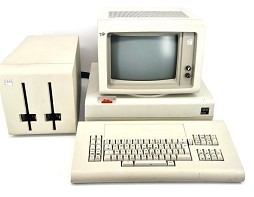
\includegraphics{./part-0/apparaetle.jpg}
% \end{center}

\begin{minipage}[c]{0.42\textwidth}
  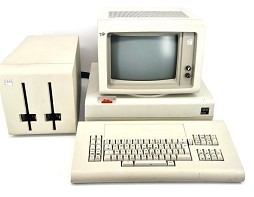
\includegraphics[width=\linewidth]{./part-0/apparaetle.jpg}
\end{minipage}
\hfill
\begin{minipage}[c]{0.42\textwidth}
  \raggedleft
  {\itshape The authors}
\end{minipage}




%% --
\contentsheader
\tableofcontents
\newpage
%% --
\symbolsheader
% !TEX root = ../LN-Book-New.tex

%% --

%% --
\chapter*{List of Symbols}
%\specialchapheader{\chapter*{List of Symbols}}{List of Symbols}
\addcontentsline{toc}{chapter}{List of Symbols}
%\chaptermark{List of Symbols}
\thispagestyle{empty}
%% --
\begin{longtable}{p{0.35\textwidth}p{0.65\textwidth}}%p{0.3\textwidth}}
%% --
$E_{\mathbb{R}}$, $E_{\mathbb{C}}$ & real, complex Banach lattice \\ % \\ % & \\
$E_{+}$ & positive cone of an ordered vector space \\ % \\ % & \\
$E'$ & dual Banach space\\ % \\ % & \\
$E^{*}$ & semigroup dual \\ % \\ % & \\
$m(E)$, $\ell^\infty(E)$  & bounded $E$-valued sequences \\
$E_{\F}$ & $\F$-product of $E$; see Part-I, Section~\ref{subsec:a1-3.7} \\% \\ % & \\
$E_{\F}^{\TT}$ & $\F$-product of $E$ with respect to the semigroup $\TT$ (l.c.) \\ % \\ % & \\
$E_f$ & see Part-III, Section~\ref{sec:c1-4}\\%Chapter 1.4 \\ % &  \\
$(E,\phi)$ &  (l.c.) \\ % & \\
$E \otimes F$ & tensor product \\ % \\ % & \\
$\LE$ & bounded linear operators on $E$ \\ % \\ % & \\
$\ZE$ & center of $E$ \\ % \\ % & \\
$E_n$ & n-th Sobolev space \\ % \\ % & \\
$\BH$ & W*-algebra of all bounded linear operators on $H$ \\ % \\ % & \\
$S(M)$ & state space of a \CA-algebra $M$ \\ % \\ % & \\
$M_+$ & positive cone of the \CA-algebra $M$ \\ % & \\
$M_*$ & predual of a \WA-algebra M\\ % & \\
$M^{sa}$ & self-adjoint part of a \CA-algebra\\ % & \\
$M_n$ & \CA-algebra of all $n \times n$-matrices \\ % & \\
$AC$ & absolutely continuous functions \\ % & \\
$BV$ & functions of bounded variation \\ % & \\
$K$ & compact topological space \\ % & \\
$X$ & locally compact topological space \\ % & \\
$C(K)$, $C(K,E)$ & continuous functions (with values in $E$) \\ % & \\
$C_{c}(X)$ & continuous functions with compact support \\ % & \\
$C_{0}(X)$ & continuous functions vanishing at infinity \\ % & \\
$C^{b}(X)$ & bounded continuous functions \\ % & \\
$C_{bu}(X)$ & bounded uniformly continuous functions \\ % & \\
$C^{n}$, $C^{(n)}$ & continuous differentiable functions ($n$-times) \\ % & \\
$C_{c}^{\infty}(\mathbb{R}^{n})$ & infinitely differentiable functions with compact support \\ % & \\
$L^{p}(\mu)$ & p-integrable functions \\ % & \\
$\mathcal{S}(\mathbb{R}^n)$ & Schwartz space \\ % & \\
$M(X)$ & regular Borel measures \\ % & \\
$M_{b}(X)$ & bounded regular Borel measures \\ % & \\
$\TT = (T(t))_{t \geq 0}$ & (one-parameter) semigroup \\ % & \\
$T_{|}$ & subspace (reduced) semigroup \\ % & \\
$T_{/}$ & quotient semigroup \\ % & \\
$\Fix{\TT}$ & fixed space of $\TT$ \\ % & \\
$A$ & generator of a $C_{0}$-semigroup\\ % & \\
$A'$ & adjoint operator of $A$\\ % & \\
$A^*$ & adjoint generator \\ % & \\
$\sigma(A)$ & spectrum of $A$\\ % & \\
$\rho(A)$ & resolvent set of $A$\\ % & \\
$\sigma_{ess}(A)$ & essential spectrum of $A$\\ % & \\
$\sigma_{b}(A)$ & boundary spectrum of $A$\\ % & \\
$P{\sigma}(A)$ & point spectrum of $A$\\ % & \\
$P{\sigma_b}(A)$ & boundary point spectrum \\ % & \\
$A\sigma(A)$ & approximate point spectrum of $A$\\ % & \\
$R{\sigma}(A)$ & residual spectrum \\ % & \\
$\omega_{0}$; $\omega_{0}(A)$; $\omega_{0}(\TT)$; $\omega_{0}(T(t))$ & growth bound \\ % & \\
$s(A)$ & spectral bound \\ % & \\
$\omega_I(A)$ & growth bound of the solution of the (ACP) \\ % & \\
$\omega(f)$ & growth bound of $T(\cdot)f$ \\ % & \\
$r(T)$ & spectral radius of $T$\\ % & \\
$\omega_{ess}(\TT)$ & essential growth bound of $\TT$\\ % & \\
$r_{ess}(T)$ & essential spectral radius of $T$\\ % & \\
$R(\lambda,A)$ & resolvent operator of $A$\\ % & \\
$I^{d}$, $\{I^{d}\}^{dd}$ & orthogonal band of $I$ (of $I^{d}$) \\ % & \\
$\wedge$ & infimum \\ % & \\
$\vee$ & supremum \\ % & \\
$|T|$ & modulus of a regular operator \\ % & \\
$\hat{f}$, $\check{f}$ & Fourier (inverse Fourier) transformation \\ % & \\
$\diff{p(f)}$ & subdifferential of $p$ in $f$ \\ % & \\
$\diff{N(f)}$ & subdifferential of the norm in $f$ \\ % & \\
$\diff{N^{+}}(f)$ & subdifferential of the canonical half-norm in $f$ \\ % & \\
$\Image{T}$ & range of $T$\\ % & \\
$\Kern{T}$ & null-space of $T$\\ % & \\
$\Im \, z$ & imaginary part of $z$ \\ % & \\
$\Re \, z$ & real part of $z$\\ % & \\
$\text{Re(f)}$, $\text{Im(f)}$ &  see Part-III, Section~\ref{sec:c1-7} \\ % & \\
$\text{Re\,T}$, $\text{Im\,T}$ & (l.c.) \\ % & \\
$\bar{f}$ & complex conjugate of $f$ \\ % & \\
$S_{f}$ & signum operator with respect to $f$ \\ % & \\
$\sign(f)$ & signum of $f$  \\ % & \\
$f^{[n]}$ & see Part-II, Chapter 3, 2.2 \& Part-III, Chapter 3, 2.1 \\ % & \\
$|f|$ & absolute value of $f$ \\ % & \\
$f^{+}$ & positive part of $f$ \\ % & \\
$f^{-}$ & negative part of $f$ \\ % & \\
$\Id$ & identity operator \\ % & \\
$M_{p}$ & multiplication operator \\ % & \\
$\1$ & function identically 1 \\ % & \\
$\1_{B}$ & characteristic function of the set $B$ \\ % & \\
$\delta_{x}$ & Dirac measure in $x$ \\ % & \\
$\text{tr}$ & trace \\ % & \\
$\text{span}\,M$ & linear subspace generated by $M$ \\ % & \\
$S(\alpha)$ & sector in the complex plane \\ % & \\
$(ACP)$ & abstract Cauchy problem \\ % & \\
$(P)$ & positive minimum principle \\ % & \\
%$(P')$ & see Part-II, Chapter 2, 1.21 \\ % & \\
$(K)$ & Kato's (equality) inequality \\ % & \\
$(RCP)$ & retarded Cauchy problem \\ % & \\
$(RE)$ & retarded equation \\ % & \\
$(T)$ & translation property \\ % & \\
\end{longtable}
%% --

% %% --
\mainmatter
\pagestyle{headings}
%% --
%% -- Part-A
\begin{partbacktext}
\part[One-parameter Semigroups on Banach Spaces]{One-parameter Semigroups on Banach Spaces }
%% -- Einleitungstext des Teils (Rückseite des Teil-Titelblatts),
%% -- übernommen aus LN-Contract-Springer/cover-teaser/Teaser.tex, 23.10.2026.
This part outlines the general framework of the theory of one-parameter semigroups of bounded linear operators on Banach spaces, paying particular attention to structures relevant to positivity.
Rather than providing a self-contained treatment, the focus is on establishing notation, recalling key definitions and results, and collecting standard examples and constructions that recur throughout the book.
Topics include the abstract Cauchy problem, perturbation and characterization results, and spectral and asymptotic theory.
This material forms the foundation for the subsequent parts, in which positivity plays a central role and Banach lattices are the primary objects of study.
\end{partbacktext}
%\setcounter{chapter}{0}

 
    % !TEX root = ../LN-Book-New.tex
%% --
%% -- Stand: 2026-03-15
%% -- 
%%\setcounter{section}{0}
%% --
\chapternopage{Basic Results on Semigroups on Banach Spaces}\label{chap:a1}%
\chaptermark{Basic Results on Banach Spaces}
\thispagestyle{empty}
%% --
{\Large
\vspace*{-.75cm}
by \\[.25em]
Rainer Nagel and Ulf Schlotterbeck 
\vspace{.75cm}
\\
}
%% --
Since the basic theory of one-parameter semigroups can be found in several excellent books (\eg \textcite{davies:1980}, \textcite{goldstein:1985a}, \textcite{pazy:1983} or \textcite{hillephillips:1957}), we do not want to give a self-contained introduction to this subject here.
It may however be useful to fix our notation, to collect briefly some important definitions and results (Section~\ref{sec:a1-1}), to present a list of \emph{standard examples} in Section~\ref{sec:a1-2} %(Section 2) 
and to discuss standard constructions of new semigroups from a given one in Section~\ref{sec:a1-3}.

In the entire chapter we denote by $E$ a (real or) complex Banach space and consider one-parameter semigroups of bounded linear operators $T(t)$ on $E$.
By this we understand a subset $\{T(t) \colon  t \in \R_{+}\}$ of\/ $\LE$, usually written as $(T(t))_{t\geq0}$, such that
%% --
\begin{align*}
	T(0) &= \Id, \\
	T(s+t) &= T(s) \cdot T(t) \text{ for all $s$, $t \in \R_{+}$.}
\end{align*}
%% --
In more abstract terms this means that the map $ \tau \colon t \mapsto T(t)$ is a homomorphism from the additive semigroup $(\R_{+},+)$ into the multiplicative semigroup $(\LE,\cdot)$.
Similarly, a one-parameter group $(T(t))_{t\in\R}$ is a homomorphism from the group  $(\R,+)$ to $(\LE,\cdot)$.
%% --
\section{Standard Definitions and Results}\label{sec:a1-1}%
%% -- 
We consider a one-parameter semigroup $(T(t))_{t \geq 0}$ on a Banach space $E$ and observe that the domain $\R_{+}$ and the range $\LE$ of the (semigroup) homomorphism $\tau $, $ t \mapsto T(t)$ are topological semigroups for the natural topology on $\R_{+}$ and any one of the standard operator topologies on $\LE$.
We single out the strong operator topology on $\LE$ and require $\tau$ to be continuous.
%% --
\begin{definition}\label{def:a1-1.1}
A one-parameter semigroup $(T(t))_{t\geq0}$ is called \emph{strongly continuous} if the map $t \mapsto T(t)$ is continuous for the strong operator topology on $\LE$, \eg
%% --
\[
	\lim_{t\to t_{0}} \|T(t)f - T(t_{0})f\| = 0
\]
%% --
for every $f \in E$ and $t_{0} \geq 0$.
\end{definition}
%% --
Clearly one defines in a similar way \emph{weakly continuous}, \resp \emph{uniformly continuous} (compare Definition~\ref{def:a2-1.19}) semigroups, but since we concentrate on the strongly continuous case we agree on the following terminology.
%% --
\begin{quote}
\textit{If not stated otherwise, a \emph{semigroup} is a strongly continuous one-parameter semigroup of bounded linear operators. }
\end{quote}
\index{semigroup}
%% --
Next we collect a few elementary facts on the continuity and boundedness of one-parameter semigroups.
%% --
\begin{remarks}\label{rem:a1-1.2}
%% --
\begin{enumerate}[\upshape(i), wide, labelindent=.25em]

\item 
A one-parameter semigroup $(T(t))_{t \geq 0}$ on a Banach space $E$ is strongly continuous if and only if for any $f \in E$ it is true that $T(t)f \to f$ as $t \to 0$.

\item 
For every strongly continuous semigroup there exist constants $ M \geq 1 $ and $ \omega \in \R $, such that 
$ \lVert T(t) \rVert \leq M \cdot \eu^{ \omega t} $ for every $  t \geq 0 $.

\item If\/ $ T(t)_{t\geq0} $ is a one-parameter semigroup such that $ \lVert T(t) \rVert $ is bounded for
$ 0 < t \leq \delta $ then it is strongly continuous if and only if\/ $ \lim_{t\to0} T(t)f = f $ for every $ f $ in a total subset of\/ $ E $.

\end{enumerate}
\end{remarks}
%% --
The exponential estimate from Remark~\ref{rem:a1-1.2}\,(ii) for the growth of\/ $ \lVert T(t) \rVert $ can be used to define an important characteristic of the semigroup.
%% --
\begin{definition}\label{def:a1-1.3}
By the \emph{growth bound} (or type) of the semigroup $ T(t)_{t\geq0} $ we understand the number $ \omega_{0} $,
\index{growth bound}
%% --
%\begin{equation}\label{eq:a1-1.1}
%\begin{split}
%	\omega_{0} & \coloneq \inf \{ \omega \in \R   \colon \text{there exists $ M \in \R_{+} $  
% 		such that $\|T(t)\| \leq M \cdot  \eu^{\omega t}$  for  $t \geq 0$} \} \\
%	& = \lim_{t\to\infty} \frac{1}{t}\log\|T(t)\| = \inf_{t>0} \frac{1}{t}\log\|T(t)\| .
%\end{split}
%\end{equation}
\begin{equation}\label{eq:a1-1.1}
\begin{aligned}
    \omega_{0} & \coloneq \inf \bigl\{ \omega \in \R \colon \text{there exists } %\exists\,
         M \in \R_{+} \text{ such that }
        \|T(t)\| \leq M \eu^{\omega t} \ (t \geq 0) \bigr\} \\
    & = \lim_{t\to\infty} \frac{1}{t}\log\|T(t)\|
      = \inf_{t>0} \frac{1}{t}\log\|T(t)\| .
\end{aligned}
\end{equation}
%% --
\end{definition}
%% --
Particularly important are semigroups such that for every $t \geq 0$ we have $\|T(t)\| \leq M$ (\emph{bounded semigroups}) or $\|T(t)\| \leq 1$ (\emph{contraction semigroups}).
In both cases we have $\omega_{0} \leq 0$.
\index{semigroup!contraction semigroup}

It follows from the subsequent examples and from Definition~\ref{def:a1-1.3} that $\omega_{0}$ may be any number $ -\infty \leq \omega < +\infty$.
Moreover the reader should observe that the infimum in Definition~\ref{def:a1-1.3} need not be attained and that $M$ may be larger than $1$ even for bounded semigroups.
%% --
\begin{examples}\label{ex:a1-1.4}
%% --
\begin{enumerate}[\upshape(i), wide, labelindent=.25em]

\item 
Take 
\[
	E = \C^{2}, \quad
	A = \begin{pmatrix}0 & 1\\0 & 0\end{pmatrix} 
	\quad \text{and} \quad 
	T(t) =  \eu^{tA} = \begin{pmatrix}1 & t\\0 & 1\end{pmatrix} .
\]
%
Then for the $\ell^{1}$-norm on $E$ we obtain $\|T(t)\| = 1 + t$, hence $(T(t))_{t\geq0}$ is an unbounded semigroup having growth bound $\omega_{0} = 0$.

\item 
Take $E = L^1(\R)$ and for $f \in E$, $t \geq 0$ define
%% --
\begin{align*}
T(t)f(x) \coloneq 
	\begin{cases}
		2\cdot f(x+t) & \text{if } x \in [-t,0] \\
		f(x+t) & \text{otherwise}.
	\end{cases}
\end{align*}
%% --
Each $T(t)$, $t > 0$, satisfies $\|T(t)\| = 2$ as can be seen by taking $f \coloneq  \1_{[0,t]}$.
Therefore $(T(t))_{t \geq 0}$ is a strongly continuous semigroup which is bounded, hence has $\omega_{0} = 0$, but the constant $M$ in Eq.~\myeqpageref{eq:a1-1.1} cannot be chosen to be $1$.

\end{enumerate}
\end{examples} 
%% --
The most important object associated to a strongly continuous semigroup $(T(t))_{t\geq0}$ is its \emph{generator} which is obtained as the (right) derivative of the map $t \mapsto T(t)$ at $t = 0$.
\index{generator}
Since for strongly continuous semigroups the functions $t \mapsto T(t)f$, $f \in E$, are continuous but not always differentiable, we have to restrict our attention to those $f \in E$ for which the desired derivative exists.
We then obtain the \emph{generator} as a not necessarily everywhere defined operator.
%% --
% \begin{definition}\label{def:a1-1.5}
% To every semigroup $(T(t))_{t \geq 0}$ there belongs an operator $(A,D(A))$, called the \emph{generator} and defined on the \emph{domain}
% %% --
% \begin{align*}
% 	D(A) \coloneqq{} & \left\{ \, f \in E \colon \lim_{h\to0} \frac{T(h)f - f}{h} 
% 	\text{ exists in $E$ } \right\} \text{ by} \\
% 	Af \coloneqq{} & \lim_{h\to0} \frac{T(h)f - f}{h} \quad (f \in D(A)).
% \end{align*}
% %% --
% \end{definition}
%% --
\begin{definition}\label{def:a1-1.5}
To every semigroup $(T(t))_{t \geq 0}$ there belongs an operator $(A,D(A))$, 
called the \emph{generator}, defined on the \emph{domain}
\begin{align*}
    D(A) &\coloneq \left\{ f \in E \colon \lim_{h\to0} \frac{1}{h} (T(h)f - f)
             \text{ exists in } E \right\}
\end{align*}
by
\begin{align*}
    Af &\coloneq \lim_{h\to0} \frac{1}{h} (T(h)f - f) \quad (f \in D(A)).
\end{align*}
\end{definition}
%% --
Clearly, $D(A)$ is a linear subspace of\/ $E$ and $A$ is linear from $D(A)$ into $E$.
Only in certain special cases (see Section~\ref{subsec:a1-2.1}) the generator
is everywhere defined and therefore bounded (use Proposition~\ref{prop:a1-1.9}\,(ii)). 
In general, the precise extent of the domain $D(A)$ is essential for the characterization of the generator.
But since the domain is canonically associated to the generator of a semigroup, we shall write in most cases $A$ instead of\/ $(A,D(A))$.
As a first result we collect some information on the domain of the generator.
%% --
\begin{proposition}\label{prop:a1-1.6}
For the generator $A$ of a semigroup $(T(t))_{t \geq 0}$ on a Banach space~$E$ the following assertions hold.
%% --
\begin{enumerate}[\upshape(i)]
\item
If\/ $f \in D(A)$, then $T(t)f \in D(A)$ for every $t \geq 0$.

\item
The map $t \mapsto T(t)f$ is differentiable on $\R_{+}$ if and only if\/ $f \in D(A)$.
In that case one has
%% --
\begin{equation}\label{eq:a1-1.2}
    \frac{\diff{}}{\dt} T(t)f = AT(t)f = T(t)Af .
\end{equation}
%% --
\item
For every $f \in E$ and $t > 0$ the element $\int_0^t T(s)f \ds$ belongs to $D(A)$ and one has
%% --
\begin{equation}\label{eq:a1-1.3}
    A \mleft( \int_0^t T(s)f \ds \mright) = T(t)f - f  .
\end{equation}
%% --
\item
If\/ $f \in D(A)$, then
%% --
\begin{equation}\label{eq:a1-1.4}
    \int_0^t T(s)Af \ds = T(t)f - f  .
\end{equation}
%% --
%% --
\item
The domain $D(A)$ is dense in $E$.
\end{enumerate}
%% --
\end{proposition}
%% --
The identity Eq.~\myeqpageref{eq:a1-1.2} is of great importance and shows how semigroups are related to certain Cauchy problems.
We state this explicitly in the following theorem.
%% --
\begin{theorem}\label{thm:a1-1.7}
Let $(A,D(A))$ be the generator of a strongly continuous semigroup $(T(t))_{t \geq 0}$ on the Banach space $E$.
Then the \emph{abstract Cauchy problem}
\index{abstract Cauchy problem}
%% --
\begin{equation}\label{eq:a1-1.5.ACP} \tag{ACP}
\frac{d}{\dt}\xi(t) = A\xi(t), \quad \xi(0) = f_{0}
\end{equation}
%% --
has for every $f_{0} \in D(A)$ a unique solution $\xi \colon \R_{+} \to D(A)$ in $C^1(\R_{+},E)$.
In fact, this solution is given by $\xi(t) \coloneq T(t)f_{0}$.
\end{theorem}
%% --
For more on the relation of semigroups to abstract Cauchy problems we refer to Section~\ref{sec:a2-1}.
Here we only point out that the above theorem implies that a semigroup is uniquely determined by its generator.

While the generator is bounded only for uniformly continuous semigroups (see Section~\ref{sec:a1-2} below), it always enjoys a weaker but useful property.
%% --
\begin{definition}\label{def:a1-1.8}
An operator $B$ with domain $D(B)$ on a Banach space $E$ is called \emph{closed} if\/ $D(B)$ endowed with the \emph{graph norm}
%% --
%\[
\begin{equation*}\label{eq:a1-1.8}
	\|f\|_{B} \coloneq \|f\| + \|Bf\|
\end{equation*} 
%\]
%% --
becomes a Banach space.
Equivalently, $(B,D(B))$ is closed if and only if its \emph{graph} $\{(f,Bf) \colon f \in D(B)\}$ is closed in $E \times E$, \ie
%% --
\[
    (f_{n}) \text{ in } D(B), f_{n} \to f \text{ and } Bf_{n} \to g \text{ implies } f \in D(B) \text{ and } Bf = g.
\]
%% --
\end{definition}
%% --
It is clear from this definition that the \emph{closedness} of an operator $B$ depends very much on the size of the domain $D(B)$.
For example, a bounded and densely defined operator $(B,D(B))$ is closed if and only if\/ $D(B) = E$.

On the other hand it may happen that $(B,D(B))$ is not closed but has a closed \emph{extension} $(C,D(C))$, \ie  $ D(B) \subseteq D(C)$ and $Bf = Cf $ for every $f \in D(B)$.
In that case, $B$ is called \emph{closable}, a property which is equivalent to
%% --
\[
    \{f_{n} \colon n \in \N \} \subseteq D(B), f_{n} \to 0 \text{ and } Bf_{n} \to g \text{ implies } g = 0.
\]
%% --
The smallest closed extension of\/ $(B,D(B))$ will be called the \emph{closure} $\overline{B}$ with domain $D(\overline{B})$.
In other words, the graph of\/ $\overline{B}$ is the closure of\/ $\{(f,Bf) \colon f \in D(B)\}$ in $E \times E$.

Finally, we call a subset $D_{0}$ of\/ $D(B)$ a \emph{core} for $B$ if\/ $D_{0}$ is $\|\cdot\|_{B}$-dense in $D(B)$.
\index{core}
This means that a closed operator is determined (via closure) by its restriction to a core in its domain.

We now collect the fundamental topological properties of semigroup generators, their domains and their resolvents
(see also Corollary~\ref{cor:a2-1.34}).
\index{resolvent}
%% --
\begin{proposition}\label{prop:a1-1.9}
For the generator $A$ of a strongly continuous semigroup $(T(t))_{t \geq 0}$ the following hold.
%% --
\begin{enumerate}[\upshape(i)]
\item 
The generator $A$ is a closed operator.

\item
If a subspace $D_{0}$ of the domain $D(A)$ is dense in $E$ and $(T(t))$-invariant, then it is a core for $A$.
% --
\item Define 
%
\begin{align*}
	D(A^{1}) & \coloneq D(A) \\
	D(A^{n}) & \coloneq \{f \in D(A^{n-1}) \colon Af \in D(A^{n-1})\} \, \text{ for $ n \geq 2 $, }
\end{align*}
%
Then %
\[
	D(A^{\infty}) \coloneq \bigcap_{n \in \N} D(A^{n})
\]
%
is dense in $E$ and a core for $A$.
\end{enumerate}
%% --
\end{proposition}
%% --
\begin{example}\label{ex:a1-1.10}
Property (iii) above does not hold for general densely defined closed operators.
Take $E = C\interval{0,1}$, $D(B) = C^{1}\interval{0,1}$ and $Bf = q \cdot f'$ for some nowhere differentiable function $q \in C\interval{0,1}$.
Then $B$ is closed, but $D(B^{2}) = \{0\}$.
\end{example}
%% --
\begin{proposition}\label{prop:a1-1.11}
For the generator $A$ of a strongly continuous semigroup on a Banach space $E$ the following hold.
If %
\[
	 \int_{0}^{\infty}  \eu^{-\lambda t}T(t)f \dt 
\]
%
exists for every $f \in E$ and some $\lambda \in \C$, then $\lambda \in \rho(A)$ and 
%
\[
	R(\lambda,A)f = \int_{0}^{\infty}  \eu^{-\lambda t}T(t)f  \dt.
\]
%
In particular,
%% --
\begin{equation}\label{eq:a1-1.7}
R(\lambda,A)^{n+1}f 
	= \frac{(-1)^{n}}{n!}\left(\frac{\diff{ }}{\diff\lambda}\right)^{n} R(\lambda,A)f 
	= \int_{0}^{\infty}  \eu^{-\lambda t}\frac{t^{n}}{n!}T(t)f  \dt
\end{equation}
%% --
for every $f \in E$, $n \geq 0$ and $\lambda \in \C$ with $\Re(\lambda) > \omega_{0}$.
\end{proposition}
%% --
\begin{remarks}\label{rem:a1-1.12}
%% --
\begin{enumerate}[\upshape(i), wide, labelindent=.25em]
%% --
\item 
For continuous Banach space valued functions such as $t \mapsto T(t)f$ we consider the Riemann integral and define 
%% --
\[
	\int_{0}^{\infty}T(t)f  \dt 
		\quad \text{as} \quad
	\lim_{t \to \infty}\int_{0}^{t}T(s)f  \ds .
\]
%% --
Sometimes such integrals for strongly continuous semigroups are written as $\int_{a}^{b}T(t) \dt$ but understood in the strong sense.

\item 
Since the generator $(A,D(A))$ determines the semigroup $(T(t))_{t \geq 0}$ uniquely, we will speak occasionally of the \emph{growth bound of the generator} instead of the semigroup, \ie we write $\omega_{0} = \omega_{0}(A) = \omega_{0}(\TT)$ where $\TT = (T(t))_{t \geq 0}$ denotes the semigroup.
\index{growth bound!omega0@$\omega_0(A)$}
\index{generator!growth bound}

\item 
For one-parameter groups it might seem to be more natural to define the generator as the \emph{derivative} rather than just the \emph{right derivative} at $t = 0$.
This yields the same operator as the following result shows.

The strongly continuous semigroup $(T(t))_{t \geq 0}$ with generator $A$ can be extended to a strongly continuous one-parameter group $(U(t))_{t \in \R}$ if and only if\/ $-A$ generates a semigroup $(S(t))_{t \geq 0}$.
In that case $(U(t))_{t \in \R}$ is obtained as
%% --
\[
    U(t) = \begin{cases}
        T(t) & \text{for } t \geq 0 ,\\
        S(-t) & \text{for } t \leq 0 .
    \end{cases}
\]
%% --
We refer to \textcite[Proposition~1.14]{davies:1980} for the details.

\end{enumerate}
\end{remarks}
%% --
\section{Standard Examples}\label{sec:a1-2}%
\index{standard example}
%% --
In this section we list and discuss briefly the most basic examples of semigroups together with their generators.
These semigroups will reappear throughout this book and will be used to illustrate the theory.
We start with the class of semigroups mentioned after Definition~\ref{def:a1-1.1}.
%% --
\subsection{Uniformly Continuous Semigroups}\label{subsec:a1-2.1}%
\index{standard example!uniformly continuous semigroup}
%% --
It follows from elementary operator theory that for every bounded operator $A$ in  $\LE$ the sum
%% --
\[
    \sum_{n=0}^{\infty} \frac{t^{n}A^{n}}{n!} = \colon  \eu^{tA}
\]
%% --
exists and determines a unique uniformly continuous (semi)group $( \eu^{tA})_{t \in \R}$ having $A$ as its generator.
Conversely, any uniformly continuous semigroup is of this form.

If the semigroup $(T(t))_{t \geq 0}$ is uniformly continuous, then 
%
\[
	\frac{1}{t}\int_{0}^{t} T(s) \ds
\]
%
uniformly converges to $T(0)=\Id$ as $t \to 0$.
Therefore for some $t' > 0$ the ope\-rator 
%
\[
	\frac{1}{t'}\int_{0}^{t'} T(s) \ds
\]
%
is invertible and every $f \in E$ is of the form 
%
\[
	f = \frac{1}{t'}\int_{0}^{t'} T(s)g \ds
\]
%
for some $g \in E$.
But these elements belong to $D(A)$ by Eq.~\myeqpageref{eq:a1-1.3}, hence $D(A) = E$.
Since the generator $A$ is closed and everywhere defined, it must be bounded.
Remark that bounded operators are always generators of groups, not just semigroups.
Moreover, the growth bound $\omega_0$ satisfies $|\omega_0| \leq \|A\|$ in this situation.

The above characterization of the generators of uniformly continuous semigroups as the bounded operators shows that these semigroups are---at least in many aspects---rather simple objects.
%% --
\subsection{Matrix Semigroups}\label{subsec:a1-2.2}%
\index{standard example!matrix semigroup}
%% --
%% --
The above considerations especially apply in the situation $E = M_{n}(\C)$.
If\/ $n = 2$ and $A \in E$, one can derive an explicit formula for $ \eu^{tA}$. 

Let %
\[
	s = \text{trace}(A), 
	\quad 
	d = \det(A) 
	\quad \text{and} \quad
	D^{2} \coloneq \left( \frac{s^{2}}{4} - d \right).
\]
%
If   
%% --
\[
p_A(\lambda) \coloneq \det(\lambda - A) = \lambda^2-s\cdot \lambda + d 
\]
%% --
is the characteristic polynomial  of\/ $ A $, then $ p_{A}(A) = 0 $ by \emph{Cayley-Hamilton}, hence
%
\[
	\left( A - \frac{s}{2} \cdot \Id \right)^{2} = D^{2} \cdot \Id , 
\]
%
where $ \Id $ denotes the unit matrix.

Now we have to consider two cases.
%% --
\begin{description}[wide, labelindent=0em]

\item[$ D^{2} = 0 $: ] 
Then $\left( A - \frac{s}{2}  \cdot \Id \right)^{k} = D^{k} \cdot \Id = 0 $  for all $ (k \geq 2)$ and this implies 
%
\[
	  \eu^{t \cdot \left( A - s/2  \cdot \Id \right)} = \Id + t \left(  A - \frac{s}{2}  \cdot \Id \right)
\]
%
or
%
\[
	 \eu^{t A } =  \eu^{t\cdot s/2} \, \left[ \left( 1 - \frac{s}{2} \, t \right )\cdot \Id + t \cdot A \right] .
\]
%
\item[$ D^{2} \neq 0 $: ]
In this case we obtain for every $ k \in \N $
%
\begin{align*}
	\left( A - \frac{s}{2} \cdot \Id \right)^{2k}  &= D^{2k} \cdot \Id \\ 
	\left( A - \frac{s}{2}  \cdot \Id \right)^{2k+1} &=\frac{1}{D} \, D^{2k+1}\left( A - \frac{s}{2} \cdot \Id \right) .
\end{align*}
%%
Thus 
\begin{align*}
	 \eu^{t( A - 1/2  \cdot \Id )} 
		& = \sum_{k=0}^\infty \frac{t^k}{k!}\left( A - \frac{s}{2}  \cdot \Id \right)^k 
		= \sum_{ \text{k even} } (\cdots) + \sum_{ \text{k odd} } (\cdots)  \\
	&= \cosh( t D ) \cdot \Id + \frac{1}{D} \sinh( t D ) \left( A - \frac{s}{2}  \cdot \Id \right) \\
	&= \frac{ 1 }{ D } \sinh( tD )\cdot A + \left( \cosh(tD) - \frac{s}{2D} \sinh(tD) \right) \cdot \Id
\end{align*}
%% --
by using the power series representation of the hyperbolic functions $ \sinh $ and $ \cosh $.
\end{description}
%% --
As summary we obtain
%% --
\begin{equation*}\label{eq:exp-rep}
	 \eu^{tA} =
	\begin{cases}
		 \eu^{t \cdot s/2} \, \left[ \frac{1}{D} \sinh(t D)  \cdot A + 
			\left( \cosh(tD) - \frac{s}{2D} \sinh(tD) \right) \cdot \Id \right], & 
									\text{if\/ $ D \neq 0 $, } \\
		 \eu^{t \cdot s/2} \, \left[ ( 1 - \frac{s}{2} \, t )\cdot \Id + t \cdot A \right], &
									\text{if\/ $ D = 0 $.}
	\end{cases}
\end{equation*}
%% 
In case $A$ is a real $2 \times2$-matrix and if\/ $ D \neq 0 $, then 
$ D^{2} = \frac{s^{2}}{4} - d $ can be positive or negative. 
%% -- 
\begin{description}[wide,  labelindent=0em]

\item[$D^2 > 0$: ]
Since $ \sinh $  is an odd function, we can choose  $ D > 0 $ in the formula for $  \eu^{tA} $.
Furthermore, $ \sinh $ and $ \cosh $ are (by definition) linear combinations of\/ $  \eu^{tD} $ and 
$  \eu^{-tD} $ simplifying our formula (see below).

\item[$D^2 < 0$: ] 
In this case $D = \pm \im|D|$.
For $ z \in \C $ we have the following identities
%
\[
	\sinh(\im z) = \frac{1}{2}(  \eu^{\im z} -  \eu^{-\im z}) = \im \sin(z)
	\quad \text{and} \quad
	\cosh(\im z) = \frac{1}{2}(  \eu^{ \im z} +  \eu^{- \im z}) = \cos(z). 
\]
%
Hence $ \sinh $ is an odd function,  $\sinh(\im |D| t ) = \im \, \sin(t|D|)$ and 
$\cosh(\im |D| t ) = \cos(|D| t )$.
%% --
\end{description}
%% --
Here are some simple examples.
%% --
\newcommand{\ABC}{\begin{pmatrix}	0 & 1 \\ -1 & 0	\end{pmatrix}}
\newcommand{\BBC}{\begin{pmatrix}	\cos(t) & \sin(t) \\ - \sin(t) & \cos(t) \end{pmatrix}}
\newcommand{\CBC}{\begin{pmatrix}	1 & 1 \\ -1 & -1 \end{pmatrix}}
\newcommand{\DBC}{\begin{pmatrix}	1+t & t \\ - t & 1-t \end{pmatrix}}
\newcommand{\EBC}{\begin{pmatrix}	0 & 1 \\ 1 &0 \end{pmatrix}}
\newcommand{\FBC}{\begin{pmatrix}	\cosh(t) & \sinh(t) \\ \sinh(t) & \cosh(t) \end{pmatrix}}
%% --
\[
  \begin{array}{lllll}
    A= & \ABC & \implies &  \eu^{tA}= & \BBC , \\\\
    A= & \CBC & \implies &  \eu^{tA}= & \DBC , \\\\ 
    A= & \EBC & \implies &  \eu^{tA}= & \FBC  .
  \end{array}
\]
%% --
\subsection{Multiplication Semigroups}\label{subsec:a1-2.3}%
\index{standard example!multiplication semigroup}
\index{semigroup!multiplication semigroup}
%% --
Many Banach spaces appearing in applications are Banach spaces of (real or) complex valued functions over a set $X$.
%% --
As the most standard examples of these \enquote{function spaces}, we mention the space $C_{0}(X)$ of all continuous complex valued functions vanishing at infinity on a locally compact space $X$, or the spaces $L^{p}(X,\Sigma,\mu)$, $1 \leq p \leq \infty$, of all (equivalence classes of) $p$-integrable functions on a $\sigma$-finite measure space $(X,\Sigma,\mu)$.

On these function spaces $E = C_{0}(X)$, \resp $E = L^{p}(X,\Sigma,\mu)$, there is a simple way to define \emph{multiplication operators}.
% --
Take a continuous, \resp measurable function $q \colon X \to \C$ and define
%% --
\[
    M_{q}f \coloneq q \cdot f, \quad \text{\ie} \quad M_{q}f(x) 
    \coloneq q(x) 	\cdot f(x) \quad \text{for } x \in X 
\]
%% --
and for every $f$ in the \emph{maximal} domain $D(M_{q}) \coloneq \{g \in E \colon q \cdot g \in E\}$.

This natural domain is a dense subspace of\/ $C_{0}(X)$, \resp $L^{p}(X,\Sigma,\mu)$, for $1 \leq p < \infty$.
Moreover, $(M_{q},D(M_{q}))$ is a closed operator.
This is easy in case $E = C_{0}(X)$.

For $E = L^{p}(X,\Sigma,\mu)$, $1 \leq p < \infty$, we consider a sequence $(f_{n})$ in  $E$ such that 
%
\[
	\lim_{n \to \infty} f_{n} = f \in E \text{ and } \lim_{n \to \infty} qf_{n} = \colon g \in E .
\]
%
Choose a subsequence $(f_{n(k)})_{k \in \N}$ such that 
%
\[
	\lim_{k \to \infty} f_{n(k)}(x) = f(x) \text{ and } \lim_{k \to \infty} q(x)f_{n(k)}(x) = g(x)
\]
for $\mu$-almost every $x \in X$.
Then $g = q \cdot f$ and $f \in D(M_{q})$, \ie $M_{q}$ is closed.

For such multiplication operators many properties can be checked quite directly.
For example, the following statements are equivalent.
%% --
\begin{enumerate}[\upshape (a)]
\item 
$M_{q}$ is bounded.

\item 
$q$ is ($\mu$-essentially) bounded.
\end{enumerate}
%% --
One has $\|M_{q}\| = \|q\|_{\infty}$ in this situation.
Observe that on spaces $C(K)$, $K$ compact, there are no densely defined, unbounded multiplication operators.
\index{operator!multiplication}

By defining the multiplication semigroups
%% --
\[
    T(t)f(x) \coloneq \exp(t \cdot q(x))f(x), \quad x \in X, f \in E,
\]

%% --
one obtains the following characterizations.
%% --
\begin{proposition*}\label{prop:a1-2.3}
%% --
Let $M_{q}$ be a multiplication operator on $E = C_{0}(X)$ or $E = L^{p}(X,\Sigma,\mu)$, $1 \leq p < \infty$.
Then the properties \upshape(a) and \upshape(b), \resp \upshape(a') and \upshape(b'), are equivalent.
%% --
\begin{enumerate}[labelwidth=2em, labelsep=0.5em, leftmargin=3em, align=left]
\item[\upshape (a)] 
	$M_{q}$ generates a strongly continuous semigroup.

\item[\upshape (b)]
	$\sup\{\Re(q(x)) \colon x \in X \} < \infty$.

\item[\upshape(a')] 
	$M_{q}$ generates a uniformly continuous semigroup.

\item[\upshape(b')] 
	$\sup\{|q(x)| \colon x \in X \} < \infty$.
\end{enumerate}
%% --
\end{proposition*}
%% --
As a consequence one computes the growth bound of a multiplication semigroup as
%% --
\[
    \omega_{0} = \sup\{\Re(q(x)) \colon x \in X\} 
\]
%% --
in the case $E = C_{0}(X)$ and 
%% --
\[
    \omega_{0} = \mu\text{-ess-}\sup\{\Re(q(x)) \colon x \in X\} 
\]
%% --
in the case  $E = L^{p}(\mu)$.
It is a nice exercise to characterize those multiplication operators which generate strongly continuous groups.

We point out that the above results cover the cases of sequence spaces such as $c_{0}$ or $\ell^{p}$, $1 \leq p < \infty$.
An abstract characterization of generators of multiplication semigroups will be given in Part-III, Theorem~\ref{thm:c2-5.13}.
%% --
\subsection{Translation (Semi)Groups}\label{subsec:a1-2.4}%
\index{standard example!translation semigroup}
\index{translation semigroup|(}
\index{semigroup!translation semigroup}
%% --
Let $E$ be one of the following function spaces $C_{0}(\R_{+})$, $C_{0}(\R)$, $L^{p}(\R_{+})$ or $L^{p}(\R)$ for $1 \leq p < \infty$.
Define $T(t)$ to be the (left) translation operator
%% --
\[
    T(t)f(x) \coloneq f(x+t)
\]
%% --
for $x$, $ t \in \R_{+}$, \resp $x, t \in \R$ and $f \in E$.
Then $(T(t))_{t \geq 0}$ is a strongly continuous semigroup, \resp group of contractions on $E$ and its generator is the first derivative $\frac{\diff{}}{\dx}$ with \emph{maximal} domain.
In order to be more precise we have to distinguish the cases $E = C_{0}$ and $E = L^{p}$.
%% -- 

The generator of the translation (semi)group on $E = C_{0}(\R_{+})$ is 
%% --
\begin{align*}
    Af & \coloneq \frac{\diff{}}{\dx}f = f' \\
    D(A) &\coloneq \{f \in E \colon f \text{ differentiable and } f' \in E\}.
\end{align*}
%% --
\begin{proof}
For $f \in D(A)$ it follows that for every $x \in \R_{(+)}$
%% --
\[
    \lim_{h \to 0} \frac{T(h)f(x) - f(x)}{h} = \lim_{h \to 0} \frac{f(x+h) - f(x)}{h} \text{ exists}
\]
%% --
(uniformly in $x$) and coincides with $Af(x)$.
Therefore $f$ is differentiable and $f' \in E$.

On the other hand, take $f \in E$ differentiable such that $f' \in E$.
Then
%% --
\[
    \left|\frac{f(x+h) - f(x)}{h} - f'(x)\right| \leq \frac{1}{h}\int_{x}^{x+h}|f'(y) - f'(x)| \dy,
\]
%% --
where the last expression tends to zero uniformly in $x$ as $h \to 0$.
Thus $f \in D(A)$ and $f' = Af$.
\end{proof}
%% --
The generator of the translation (semi)group on $E = L^{p}(\R_{+})$, $1 \leq p < \infty$, is
%% --
\begin{align*}
    Af &\coloneq \frac{\diff{}}{\dx}f = f', \\
    D(A) &\coloneq \{f \in E \colon f \text{ absolutely continuous}, f' \in E\}.
\end{align*}
%% --
\begin{proof}
Take $f \in D(A)$ such that $\lim_{h \to 0} \frac{1}{h}(T(h)f - f) = g \in E$.
Since integration is continuous, we obtain for every $a$, $b \in \R_{(+)}$ that
%% --
\begin{equation*}\label{eq:a1-2.1}
(*) \quad \frac{1}{h}\int_{b}^{b+h} f(x) \dx - \frac{1}{h}\int_{a}^{a+h} f(x) \dx = \int_{a}^{b} \frac{f(x+h) - f(x)}{h} \dx
\end{equation*}
%% --
converges to $\int_{a}^{b} g(x) \dx$ as $h \to 0+$.
But for almost all $a$, $b$ the left hand side of\/ $(*)$ converges to $f(b) - f(a)$.
By redefining $f$ on a nullset we obtain
%% --
\[
    f(y) = \int_{a}^{y} g(x)\dx + f(a), \quad y \in \R_{(+)},
\]
%% --
which is an absolutely continuous function whose derivative is (almost everywhere) equal to $g$.

On the other hand, let $f$ be absolutely continuous such that $f' \in L^{p}$.
Then
% %% --
% \begin{align*}
%     \lim_{h \to 0} \int{\left|\frac{f(x+h) - f(x)}{h} - f'(x)\right|^{p} \dx} 
%     &= \lim_{h \to 0} \int {\left|\frac{1}{h}\int_{0}^{h} (f'(x+s) - f'(x)) \ds\right|^{p} \dx }\\
%     &= \lim_{h \to 0} \int {\left|\int_{0}^{1} (f'(x+uh) -  \int f'(x)) \du\right|^{p} \dx }\\
%     &\leq \lim_{h \to 0}{ \int \int_{0}^{1} |f'(x+uh) - f'(x)|^p \du \dx }\\
%     & = {\int_{0}^{1}} \displaystyle{\lim_{h \to 0}} {\int|f'(x+uh) - f'(x)|^{p} \dx \du = 0},
% \end{align*}
%% --
\begin{align*}
    &\lim_{h \to 0} \int\left|\frac{f(x+h) - f(x)}{h} - f'(x)\right|^{p} \dx \\
    &\quad= \lim_{h \to 0} \int \left|\frac{1}{h}\int_{0}^{h} (f'(x+s) - f'(x)) \ds\right|^{p} \dx \\
    &\quad= \lim_{h \to 0} \int \left|\int_{0}^{1} (f'(x+uh) - f'(x)) \du\right|^{p} \dx \\
    &\quad\leq \lim_{h \to 0} \int \int_{0}^{1} |f'(x+uh) - f'(x)|^p \du \dx \\
    &\quad= \int_{0}^{1} \lim_{h \to 0} \int|f'(x+uh) - f'(x)|^{p} \dx \, \du = 0,
\end{align*}
%% --
hence $f \in D(A)$.
\end{proof}
\index{translation semigroup|)}
%% --
\subsection{Rotation Groups}\label{subsec:a1-2.5}%
\index{standard example!rotation group}
\index{semigroup!rotation semigroup}
%% --
On $E = C(\Gamma)$, \resp $E = L^{p}(\Gamma,m)$, $1 \leq p < \infty$, $m$ Lebesgue measure we have canonical groups defined by rotations of the unit circle $\Gamma$ with a certain period, \ie for $0 < \tau \in \R$ the operators
%% --
\[
    R_{\tau}(t)f(z) \coloneq f( \eu^{2\pi \im t/\tau}\cdot z), \quad z \in \Gamma
\]
%% --
yield a group $(R_{\tau}(t))_{t \in \R}$ having period $\tau$, \ie $R_{\tau}(\tau) = \Id$.
As in Section~\ref{subsec:a1-2.4} one shows that its generator has the form
%% --
\begin{align*}
    D(A) &= \{f \in E \colon f \text{ absolutely continuous}, f' \in E\}, \\
    Af(z)&= (2\pi \im/\tau) \cdot z \cdot f'(z).
\end{align*}
%% --
An isomorphic copy of the group $(R_{\tau}(t))_{t \in \R}$ is obtained if we consider 
%% --
\[
E = \{f \in C\interval{0,1} \colon f(0) = f(1)\}
\]
%% -- 
\resp 
%% --
\[
E = L^{p}(\interval{0,1})
\]
%% --
and the group of \emph{periodic translations}
%% --
\[
    T(t)f(x) \coloneq f(y) \quad \text{for $y \in \interval{0,1}, y = x+t \bmod 1$} 
\]
%% --
with generator
%% --
\[
    D(A) \coloneq \{f \in E \colon f \text{ absolutely continuous, $f' \in E$, $Af \coloneq f'$}. \}
\]
%% --
\subsection{Nilpotent Translation Semigroups}\label{subsec:a1-2.6}%
\index{standard example!nilpotent translation semigroup}
\index{semigroup!nilpotent semigroup}
\index{translation semigroup}
%% --
Take $E = L^{p}([0,\tau],m)$ for $1 \leq p < \infty$ and define
%% --
\[
    T(t)f(x) \coloneq \begin{cases}
        f(x+t) & \text{if } x+t \leq \tau \\
        0 & \text{otherwise.}
    \end{cases}
\]
%% --
Then $(T(t))_{t\geq 0}$ is a semigroup satisfying $T(t) = 0$ for $t \geq \tau$.
Its generator is still the first derivative $A = \frac{d}{\dx}$, but with domain 
%% --
\[
D(A) = \{f \in E \colon f \text{ absolutely continuous}, f' \in E, f(\tau) = 0\}.
\]
%% --
In fact, if\/ $f \in D(A)$, then $f$ is absolutely continuous with $f' \in E$.
By Proposition~\ref{prop:a1-1.6}\,(i), it follows that $T(t)f$ is absolutely continuous and hence $f(\tau) = 0$.
%% --
\subsection{One-dimensional Diffusion Semigroup}\label{subsec:a1-2.7}%
\index{standard example!one-dimensional diffusion semigroup}
%% --
For the second derivative 
%% --
\[
    Bf(x) \coloneq \frac{\mathrm{d}^{2}}{\dx^{2}}f(x) = f''(x)
\]
%% --
we take the domain
%% --
\[
    D(B) \coloneq \{f \in C^{2}\interval{0,1} \colon f'(0) = f'(1) = 0\}
\]
%% --
in the Banach space $E = C\interval{0,1}$.
Then $D(B)$ is dense in $C\interval{0,1}$, but closed for the graph norm.
Obviously, each function
%% --
\[
    e_{n}(x) \coloneq \cos \pi nx \quad (n \in \Z, x \in \interval{0,1})
\]
%% --
is contained in $D(B)$ and is an eigenfunction of\/ $B$ pertaining to the eigenvalue $\lambda_{n} \coloneq -\pi^{2}n^{2}$.
The linear hull $\text{span }\{e_{n} \colon n \in \Z\} = \colon E_{0}$ forms a subalgebra of\/ $D(B)$ which by the Stone-Weierstrass theorem is dense in $E$.

We now use $e_{n}$ to define bounded linear operators 
%% --
\[
	e_{n} \otimes e_{n} \colon f \mapsto \left(\int_{0}^{1} f(x)e_{n}(x) \dx \right)e_{n} 
		= ( f | e_{n} ) e_{n} %\langle f,e_{n}\rangle e_{n}
\]
%% -- 
satisfying $\|e_{n} \otimes e_{n}\| \leq 1$ and
$(e_{n} \otimes e_{n})(e_{m} \otimes e_{m}) = \delta_{n,m}(e_{n} \otimes e_{n})$ for $n \in \Z$.

For $t > 0$ we define
%% --
%\begin{align*}
%T(t) \coloneqq{}& \sum_{n \in \Z} \exp(-\pi^{2}n^{2}t) \cdot e_{n} \otimes e_{n} \\
%		={}& e_{0} \otimes e_{0} + 2\sum_{n=1}^{\infty} \exp(-\pi^{2}n^{2}t) \cdot e_{n} \otimes e_{n},
%\end{align*}
%or
%%% --
%\begin{align*}
%    T(t)f(x) &= \int_{0}^{1} k_{t}(x,y)f(x)dy \\
%    \text{where } k_{t}(x,y) &= 1 + 2\sum_{n=1}^{\infty} \exp(-\pi^{2}n^{2}t) \cos\pi nx \cos\pi ny .
%\end{align*}
%% --
\begin{align*}
T(t) \coloneqq{}& \sum_{n \in \Z} \exp(-\pi^{2}n^{2}t) \cdot e_{n} \otimes e_{n} \\
     ={}& e_{0} \otimes e_{0} 
          + 2\sum_{n=1}^{\infty} \exp(-\pi^{2}n^{2}t) \cdot e_{n} \otimes e_{n}, 
\intertext{or}
    T(t)f(x) &= \int_{0}^{1} k_{t}(x,y)\,f(y)\dy ,
\intertext{where}
    k_{t}(x,y) &= 1 + 2\sum_{n=1}^{\infty} \exp(-\pi^{2}n^{2}t) 
                  \cos(\pi nx)\cos(\pi ny).
\end{align*}
%% --
The Jacobi identity
%% --
\begin{align*}
    w_{t}(x) &\coloneq \left( \frac{1}{4\pi t}\right)^{\frac{1}{2}} \sum_{m \in \Z} \exp(-(x+2m)^{2}/4t) \\
    &= \frac{1}{2} + \sum_{n \in \N} \exp(-\pi^{2}n^{2}t) \cos\pi nx
\end{align*}
%% --
and trigonometric relations show that
%% --
\[
    k_{t}(x,y) = w_{t}(x+y) + w_{t}(x-y)
\]
%% --
which is a positive function on $\interval{0,1}^{2}$.
Therefore $T(t)$ is a bounded operator on $C\interval{0,1}$ with
%% --
\[
    \|T(t)\| = \|T(t)\1\| = \sup_{x \in \interval{0,1}} \int_{0}^{1} k_{t}(x,y)dy = 1 .
\]
%% --
From the behavior of\/ $T(t)$ on the dense subspace $E_{0}$ it follows that $(T(t))_{t \geq 0}$ with $T(0) = \Id$ is a strongly continuous semigroup on $E$ and its generator $A$ coincides with $B$ on $E_{0}$.
Finally, we observe that $E_{0}$ is a core for $(A,D(A))$ by Proposition~\ref{prop:a1-1.9}\,(ii).
Consequently, $(T(t))_{t \geq 0}$ is the semigroup generated by $B$.
%% --
\subsection{n-dimensional Diffusion Semigroup}\label{subsec:a1-2.8}%
\index{standard example!$n$-dimensional diffusion semigroup}
%% --
On $E = L^{p}(\R^{n})$, $1 \leq p \leq \infty$, the operators
%% --
\begin{align*}
    T(t)f(x) \coloneqq{}& (4\pi t)^{-n/2} \int_{\R^{n}} \exp(-|x-y|^{2}/4t)f(y)dy \\
    ={}& \mu_{t}*f(x)
\end{align*}
%% --
for $x \in \R^{n}$, $t > 0$ and 
%
\[
	\mu_{t}(x) \coloneq (4\pi t)^{-n/2} \exp(-|x|^{2}/4t)
\]
%
form a strongly continuous semigroup.

In fact, the integral exists for every $f \in L^{p}(\R^{n})$ since $\mu_{t}$ is an element of the Schwartz space $\mathcal{S}(\R^{n})$ of all rapidly decreasing smooth functions on $\R^{n}$.

Moreover,
%% --
\[
    \|T(t)f\|_{p} \leq \|\mu_{t}\|_{1}\|f\|_{p} = \|f\|_{p}
\]
%% --
by Young's inequality (\textcite[p.28]{reedsimon:1975}). Hence $\|T(t)\| \leq 1$ for every $t > 0$.

Next we observe that $\mathcal{S}(\R^{n})$ is dense in $E$ and invariant under each $T(t)$.
Therefore we can apply the Fourier transformation $\mathbf{F}$ which leaves $\mathcal{S}(\R^{n})$ invariant and yields
%% --
\[
    \mathbf{F}(\mu_{t}*f) = (2\pi)^{n/2} \mathbf{F}(\mu_{t}) \cdot \mathbf{F}(f) 
    = (2\pi)^{n/2} \hat{\mu}_{t}\cdot\hat{f}
\]
%% --
where $f \in \mathcal{S}(\R^{n})$, $\hat{f} = \mathbf{F}f \in \mathcal{S}(\R^{n})$.

In other words, $\mathbf{F}$ transforms $(T(t)\vert_{ S(\R^{n})})_{t \geq 0}$ into a multiplication semigroup on $\mathcal{S}(\R^{n})$ which is pointwise continuous for the usual topology of\/ $\mathcal{S}(\R^{n})$.
The generator, \ie the right derivative at $0$, of this semigroup is the multiplication operator
\index{operator!multiplication}
%% --
\[
    B\hat{f}(x) \coloneq -|x|^{2}\hat{f}(x) \quad (x \in \R^{n})
\]
%% --
for every $f \in \mathcal{S}(\R^{n})$.

Applying the inverse Fourier transformation and observing that the topology of\/ $\mathcal{S}(\R^{n})$ is finer than the topology induced from $L^{p}(\R^{n})$, we obtain that $(T(t))_{t \geq 0}$ is a semigroup which is strongly continuous (use Remark~\ref{rem:a1-1.2}\,(iii)).

Its generator $A$ coincides with
%% --
\[
    \Delta f(x) = \sum_{i=1}^{n} \frac{\partial^{2}}{\partial x_{i}^{2}} f(x_{1},\ldots,x_{n})
\]
%% --
for every $f \in \mathcal{S}(\R^{n})$.
Since $\mathcal{S}(\R^{n})$ is $(T(t))$-invariant, we have determined the generator on a core of its domain (see Proposition~\ref{prop:a1-1.9}\,(ii)).
In particular, the above semigroup \emph{solves} the initial value problem for the \emph{heat equation}
%% --
\[
    \frac{\partial}{\partial t} f(x,t) = \Delta f(x,t), \quad f(x,0) = f_{0}(x), \quad x \in \R^{n}.
\]
%% --
For the analogous discussion of the unitary group on $L^{2}(\R^{n})$ generated by
%% --
\[
    C \coloneq \im\Delta
\]
%% --
we refer to Section IX.7 in \textcite{reedsimon:1975}. 

%Examples analogous to Section~\ref{subsec:a1-2.7} are valid in $L^{p}\interval{0,1}$, \resp to Section~\ref{subsec:a1-2.8} in $C_{0}(\R^{n})$.
The constructions of Sections~\ref{subsec:a1-2.7} 
and~\ref{subsec:a1-2.8} carry over to $L^{p}\interval{0,1}$ 
and $C_{0}(\R^{n})$, respectively.
%% --
\section{Standard Constructions}\label{sec:a1-3}%
\index{standard construction}
%% --
Starting with a semigroup $(T(t))_{t \geq 0}$ on a Banach space $E$ it is possible to construct new semigroups on spaces naturally associated with $E$.
Such constructions will be important technical devices in many of the subsequent proofs.
Although most of these constructions are rather routine, we present below a systematic account of them for the convenience of the reader.

%In the following we always start with a semigroup $(T(t))_{t \geq 0}$ on a Banach space $E$, and denote its generator by $A$ on the domain $D(A)$.
Throughout, $(T(t))_{t \geq 0}$ denotes a $C_0$-semigroup on a Banach space $E$, with generator $A$ on $D(A)$.
%% --
\subsection{Similar Semigroups}\label{subsec:a1-3.1}%
\index{standard construction!similar semigroup}

%% --
There is an easy way how to obtain different (but isomorphic) semigroups out of a given semigroup $(T(t))_{t \geq 0}$ on a Banach space $E$.

Let $V$ be an isomorphism from $E$ onto $E$.
Then $S(t) \coloneq VT(t)V^{-1}$, $t \geq 0$, defines a strongly continuous semigroup.
If\/ $A$ is the generator of\/ $(T(t))_{t \geq 0}$, then
%% --
\[
    B \coloneq VAV^{-1} \text{ with domain } D(B) \coloneq \{f \in E \colon V^{-1}f \in D(A)\}
\]
%% --
is the generator of\/ $(S(t))_{t \geq 0}$.
%% --
\subsection{The Rescaled Semigroup}\label{subsec:a1-3.2}%
\index{standard construction!rescaled semigroup}
%% --
For fixed $\lambda \in \C$ and $\alpha > 0$ the operators
%% --
\[
    S(t) \coloneq \exp(\lambda t)T(\alpha t)
\]
%% --
yield a new semigroup having generator
%% --
\[
    B \coloneq \alpha A + \lambda \Id \text{ with } D(B) = D(A) .
\]
%% --
This \emph{rescaled semigroup} enjoys most of the properties of the original semigroup and the same is true for the corresponding generators.
However, by using this procedure certain constants associated with $(T(t))_{t \geq 0}$ and $A$ can be normalized.
For example, by this rescaling we may suppose, in many cases without loss of generality, that the growth bound $\omega_{0}$ is zero.

Another application is the following.
For $\lambda \in \C$ and $S(t) \coloneq \exp(-\lambda t)T(t)$ the formulas \eqref{eq:a1-1.3} and \eqref{eq:a1-1.4} on p.~\pageref{eq:a1-1.4} yield:
%% --
\begin{equation}\label{eq:a1-3.1}
\begin{split}
     \eu^{-\lambda t}T(t)f - f &= (A-\lambda) \int_{0}^{t}  \eu^{-\lambda s}T(s)f \ds \\[4pt]
     & \text{ or } \\[4pt]
    ( \eu^{\lambda t}-T(t))f &= (\lambda-A) \int_{0}^{t}  \eu^{\lambda(t-s)}T(s)f \ds \quad \text{for } f \in E,  
\end{split}
\end{equation}
%% --
and
%% --
\begin{equation}\label{eq:a1-3.2}
\begin{split}
     \eu^{-\lambda t}T(t)f - f &= \int_{0}^{t}  \eu^{-\lambda s}T(s)(A-\lambda)f \ds \\[4pt]
     & \text{ or } \\[4pt]
    ( \eu^{\lambda t} - T(t))f &= \int_{0}^{t}  \eu^{\lambda(t-s)}T(s)(\lambda-A)f \ds \quad \text{for } f \in D(A).  
\end{split}
\end{equation}
%% --
\subsection{The Subspace Semigroup}\label{subsec:a1-3.3}%
\index{standard construction!subspace semigroup}
\index{semigroup!subspace semigroup}
%% --
%Assume $F$ to be a closed $(T(t))$-invariant or, equivalently, $R(\lambda,A)$-invariant for 
%$\lambda \in \C$, 
%$ \Re(\lambda) > \omega_{0}$, subspace of\/ $E$.
%Then the semigroup $(T(t)_{|})_{t \geq 0}$ of all restrictions $T(t)_{|} \coloneq T(t)_{|\,F}$ is strongly continuous on $F$.
%If\/ $(A,D(A))$ denotes the generator of\/ $(T(t))_{t \geq 0}$ it follows from the $(T(t))$-invariance and closedness of\/ $F$ that $A$ maps $D(A) \cap F$ into $F$.

Assume $F$ to be a closed subspace of $E$ that is invariant under $(T(t))_{t \geq 0}$, or equivalently, under $R(\lambda, A)$ for all $\lambda \in \C$ with $\Re(\lambda) > \omega_{0}$.
Then the restricted semigroup
%% --
\[
    T_{\vert}(t) \coloneq T(t)\big|_{F}, \quad t \geq 0,
\]
%% --
is strongly continuous on $F$.
If $(A, D(A))$ denotes the generator of $(T(t))_{t \geq 0}$, it follows from the invariance and closedness of $F$ that $A$ maps $D(A) \cap F$ into $F$.

Therefore
%% --
\[
    A_{|} \coloneq A\big|_{ (D(A)\cap F)} \text{ with domain } D(A_{|}) \coloneq D(A) \cap F
\]
%% --
is the generator of\/ $(T(t)_{|})$.
%
Conversely, if\/ $F$ is a closed \emph{linear subspace} of\/ $E$ with $A(D(A) \cap F) \subseteq F$ such that 
$A_{|}$ is a generator on $F$, then $F$ is $(T(t))$-invariant.

An $A$-invariant subspace need not necessarily be $(T(t))$-invariant:
Take for example the translation group with $(T(t)f)(x) = f(x+t)$ on $E = C_{0}(\R)$ and the subspace $F \coloneq \{f \in E \colon f(x) = 0 \text{ for } x \leq 0\}$.
%% --
\subsection{The Quotient Semigroup}\label{subsec:a1-3.4}%
\index{standard construction!quotient semigroup}
%% --
%Let $F$ be a closed $(T(t))$-invariant subspace of\/ $E$ and consider the quotient space 
%$ E_{/} \coloneq \sfrac{E}{F} $ 
%with quotient map $q \colon E \to E_{/}$. 
%The quotient operators
%%% --
%\[
%    T(t)_{/}q(f) \coloneq q(T(t)f), \quad f \in E,
%\]
%%% --
%are well defined and form a strongly continuous semigroup $(T(t)_{/})_{t \geq 0}$ on $E_{/}$.
%For the generator $(A_{/},D(A_{/}))$ of\/ $(T(t)_{/})_{t \geq 0}$ the following holds:
%%% --
%\[
%    D(A_{/}) = q(D(A)) 
%    \quad \text{and} \quad 
%    A_{/}q(f) = q(Af)
%\]
%%% --
%for every $f \in D(A)$.
%Here we use the fact that every $\hat{f} \coloneq q(f) \in D(A_{/})$ can be written as
%%% --
%\[
%    \hat{f} = \int_{0}^{\infty}  \eu^{-\lambda s} \widehat{T}(s)_{/}\hat{g} \ds 
%    = \int_{0}^{\infty}  \eu^{-\lambda s}q(T(s)g) \ds 
%    = q\left(\int_{0}^{\infty}  \eu^{-\lambda s}T(s)g \ds\right) = q(h)
%\]
%%% --
%where $h \in D(A)$ and $\lambda > \omega$ (see Proposition~\ref{prop:a1-1.6}).
%In particular we point out that for every $\hat{f} \in D(A_{/})$ there exist representatives $f \in \hat{f}$ belonging to $D(A)$.
%% --
Let $F$ be a closed $(T(t))_{t \geq 0}$-invariant subspace of $E$ and consider the quotient space $E_{/} \coloneq \mfrac{E}{F}$ with quotient map $q \colon E \to E_{/}$.
The quotient operators
%% --
\[
    T_{/}(t)\,q(f) \coloneq q(T(t)f), \quad f \in E,
\]
%% --
are well defined and form a strongly continuous semigroup $\mleft(T_{/}(t)\mright)_{t \geq 0}$ on $E_{/}$.

For the generator $(A_{/}, D(A_{/}))$ of $\mleft(T_{/}(t)\mright)_{t \geq 0}$ the following holds:
%% --
\[
    D(A_{/}) = q(D(A)) 
    \quad \text{and} \quad 
    A_{/}q(f) = q(Af)
\]
%% --
for every $f \in D(A)$.
Here we use the fact that every $\hat{f} \coloneq q(f) \in D(A_{/})$ can be written as
%% --
\[
    \hat{f} = \int_{0}^{\infty} \eu^{-\lambda s} T_{/}(s)\hat{g} \, \ds 
            = \int_{0}^{\infty} \eu^{-\lambda s} q(T(s)g) \, \ds 
            = q\mleft(\int_{0}^{\infty} \eu^{-\lambda s} T(s)g \, \ds\mright) 
            = q(h)
\]
%% --
where $h \in D(A)$ and $\lambda > \omega$ (see Proposition~\ref{prop:a1-1.6}).
In particular, for every $\hat{f} \in D(A_{/})$ there exist representatives $f \in \hat{f}$ belonging to $D(A)$.
%% --
\begin{example*}\label{ex:a1-3.1}%
\index{standard example!translation semigroup}
%%
%We start with the Banach space $E = L^{1}(\R)$ and the translation semigroup $(T(t))_{t \geq 0}$ where $T(t)f(x) \coloneq f(x+t)$ (see Example~\ref{subsec:a1-2.4}).
%Then $L^{1}((-\infty,1])$ can be identified with the closed, $(T(t))$-invariant subspace
%%% --
%\[
%    J \coloneq \{f \in E \colon f(x) = 0 \text{ for } 1 < x < \infty\} .
%\]
%%% --
%There we obtain the subspace semigroup
%%% --
%\[
%    (T(t)_{|}f)(x) = \1_{(-\infty,1]}(x) \cdot f(x+t),
%\]
%%% --
%where $f \in L^{1}((-\infty,1])$, $-\infty < x \leq 1$ and $t \geq 0$.
%
%By Section~\ref{subsec:a1-2.4} and Section~\ref{subsec:a1-3.2} its generator is
%%% --
%\[
%    A_{|}f \coloneq f'
%\]
%%% --
%for $f \in D(A_{|}) \coloneq \{f \in E \colon f \in AC \text{ with } f' \in E \text{ and } f(x) = 0 \text{ for } x \geq 1\}$.
%
%Next we identify $L^{1}(\interval{0,1})$ with the quotient space \sfrac{$L^{1}((-\infty,1])$}{I} where
%
%%% --
%\[
%    I \coloneq \{f \in L^{1}((-\infty,1]) \colon f(x) = 0 \text{ for } 0 \leq x \leq 1\} .
%\]
%%% --
%Again $I$ is invariant for the restricted semigroup $(T(t)_{|})$ and the
%%% --
%quotient semigroup $(T(t)_{\vert _{/}})$ on $L^{1}(\interval{0,1})$ is the nilpotent translation semigroup as in Section~\ref{subsec:a1-2.6}.
%In particular it follows that the domain of its generator is
%%% --
%\[
%    D(A_{|_{/}}) = \{f \in L^{1}(\interval{0,1}) \colon f \in AC \text{ with } f' \in L^{1}(\interval{0,1}) \text{ and } f(1) = 0\}.
%\]
We start with the Banach space $E = L^{1}(\R)$ and the translation semigroup $(T(t))_{t \geq 0}$ where $T(t)f(x) \coloneq f(x+t)$ (see Example~\ref{subsec:a1-2.4}).
Then $L^{1}((-\infty,1])$ can be identified with the closed, 
$(T(t))_{t \geq 0}$-invariant subspace
\[
    F \coloneq \{f \in E \colon f(x) = 0 \text{ for } x > 1\}.
\]
The restricted semigroup on $F$ is given by
\[
    T_{\vert F}(t)f(x) = \mathbf{1}_{(-\infty,1]}(x) \cdot f(x+t),
    \quad f \in F,\; x \leq 1,\; t \geq 0.
\]
By Sections~\ref{subsec:a1-2.4} and~\ref{subsec:a1-3.2}, the generator 
$A_{\vert F}$ acts as $A_{\vert F}f = f'$ on the domain
\[
    D(A_{\vert F}) \coloneq \{f \in F \colon f \in AC,\; 
    f' \in F \text{ and } f(x) = 0 \text{ for } x \geq 1\}.
\]
Next, $L^{1}(\interval{0,1})$ can be identified with the quotient space 
\mfrac{F}{I}, where
\[
    I \coloneq \{f \in F \colon f(x) = 0 \text{ for } 0 \leq x \leq 1\}.
\]
Since $I$ is invariant under $\mleft(T_{\vert F}(t)\mright)_{t \geq 0}$, 
the quotient semigroup $\mleft(T_{/}(t)\mright)_{t \geq 0}$ on 
$L^{1}(\interval{0,1})$ is the nilpotent translation semigroup of 
Section~\ref{subsec:a1-2.6}.
In particular, the domain of its generator $A_{/}$ is
\[
    D(A_{/}) = \{f \in L^{1}(\interval{0,1}) \colon f \in \mathrm{AC},  
    f' \in L^{1}(\interval{0,1}) \text{ and } f(1) = 0\}.
\]
\end{example*}
%% --
\subsection{The Adjoint Semigroup}\label{subsec:a1-3.5}%
\index{standard construction!adjoint semigroup}
\index{adjoint semigroup}
\index{operator!adjoint}
%% --
The adjoint operators $(T(t)')_{t \geq 0}$ of a strongly continuous semigroup $(T(t))_{t \geq 0}$ on a Banach space $E$ form a semigroup on $E'$ which need, however, not be strongly continuous.
%% --
\begin{example*}\label{ex:a1-3.2}
%% --
Take the translation operators $T(t)f(x) = f(x+t)$ on $E = L^{1}(\R)$ (see Section~\ref{subsec:a1-2.4}) and their adjoints
%% --
\[
    T(t)'f(x) = f(x-t)
\]
%% --
on $E' = L^{\infty}(\R)$.
Then $(T(t)')_{t \in \R}$ is a one-parameter group which is not strongly continuous on $L^{\infty}(\R)$ (take any non-trivial characteristic function).
\end{example*}
%% --
Since the semigroup $(T(t)')_{t \geq 0}$ is 
obviously \emph{weak*-continuous} in the sense that 
%% --
\[
\lim_{t \to s} \langle f,(T(t)'-T(s)')\phi \rangle = 0
\]
%% --
for every $f \in E$, $\phi \in E'$ and $s$, $t \geq 0$, it is natural to associate $(T(t)')_{t \geq 0}$ its  \emph{weak*-generator}
%% --
\begin{align*}
    A'\phi &\coloneq \sigma(E',E)\text{-}\lim\frac{1}{h}(T(h)'\phi-\phi) \text{ for every } \phi \text{ in the domain} \\
    D(A') &\coloneq \{\phi \in E' \colon \sigma(E',E)\text{-}\lim\frac{1}{h}(T(h)'\phi-\phi) \text{ exists}\}.
\end{align*}
%% --
This operator coincides with the \emph{adjoint} of the generator $(A,D(A))$, \ie
%% --
\[
    D(A') = \{\phi \in E' \colon \text{there exists } \psi \in E' \text{ such that } \langle f,\psi \rangle = \langle Af,\phi \rangle \text{ for all } f \in D(A)\}
\]
%% --
and $A'\phi = \psi$.
In particular, $A'$ is a closed and $\sigma(E',E)$-densely defined operator in $E'$.

It follows that the resolvent $R(\lambda,A')$ of\/ $A'$ is $R(\lambda,A)'$ 
(\textcite[Theorem~III.5.30]{kato:1976}).
In particular, the spectra $\sigma(A)$ and $\sigma(A')$ coincide.

However, it is still necessary in some situations to have strong continuity for the adjoint semigroup.
In order to achieve this we restrict $T(t)'$ to an appropriate subspace of\/ $E'$.
%% --
\begin{definition*}[\normalfont\textcite{phillips:1954}]\label{def:a1-3.1}
The \emph{semigroup dual} of the Banach space $E$ with respect to the strongly continuous semigroup $(T(t))_{t \geq 0}$ is
%% --
\[
    E^{*} \coloneq \{\phi \in E' \colon \|\cdot\|\text{-}\lim_{t \to 0} T(t)'\phi = \phi\}.
\]
%% --
The adjoint semigroup on $E^{*}$ is given by the operators
%% --
\[
    T(t)^{*} \coloneq T(t)'_{ \vert E^{*}}, \quad t \geq 0.
\]
%% --
Since $(T(t)^{*})_{t \geq 0}$ is strongly continuous on $E^{*}$ we call its generator $(A^{*},D(A^{*}))$ the \emph{adjoint generator}.
\end{definition*}
%% --
The above definition makes sense since $E^{*}$ is norm-closed in $E'$ and $(T(t)')$-invariant.
The main point is that $E^{*}$ is still reasonably large.
In fact, since $\int_{0}^{t} T(s)'\phi  \ds$, understood in the weak sense, is contained in $E^{*}$ for every $\phi \in E'$ and $t \geq 0$, it follows that
%% --
\[
    \sup\{\langle f,\phi \rangle \colon \phi \in E^{*}, \|\phi\| \leq 1\} \leq \|f\| \leq M\cdot\sup\{\langle f,\phi \rangle \colon \phi \in E^{*}, \|\phi\| \leq1\}
\]
%% --
where $M \coloneq \lim\sup_{t \to 0} \|T(t)\|$.
In particular, $E^{*}$ separates $E$, \ie $E^{*}$ is $\sigma(E',E)$-dense in $E'$.
In addition, the norm estimate given above yields
%% --
\[
    \|T(t)^{*}\| \leq \|T(t)\| \leq M\|T(t)^{*}\| \quad \text{for all } t \geq 0.
\]
%% --
In the following proposition we describe the relation between $A^{*}$ and $A'$.
%% --
\begin{proposition*}\label{prop:a1-3.4}
For the adjoint generator $A^{*}$ of a strongly continuous semigroup $(T(t))_{t \geq 0}$ on $E$ the following assertions hold.
%% --
\begin{enumerate}[\upshape(i)]
\item 
$E^{*}$ is the $\|\cdot\|$-closure of\/ $D(A')$.

\item 
$D(A^{*}) = \{\phi \in D(A') \colon A'\phi \in E^{*}\}$.

\item 
$A^{*}$ and $A'$ coincide on $D(A^{*})$.
\end{enumerate}
\end{proposition*}
%% --
\begin{proof}
(i) Take $\phi \in D(A')$ fixed.
For every $f \in D(A)$ with $\|f\| \leq 1$ we define a continuously differentiable function
%% --
\[
    t \mapsto \xi_{f}(t) \coloneq \langle T(t)f,\phi \rangle
\]
%% --
on $\interval{0,1}$ with derivative 
%
\[
	\xi_{f}'(t) = \langle T(t)Af,\phi \rangle = \langle T(t)f,A'\phi \rangle .
\]
%
Since $\{\xi_{f}'(t) \colon t \in \interval{0,1}, f \in D(A), \|f\| \leq 1\}$ is bounded, it follows that the set
%% --
\[
    \{\xi_{f} \colon f \in D(A), \|f\| \leq 1\}
\]
%% --
is equicontinuous at $0$, \ie for every $\epsilon > 0$ there exists $0 < t_{0} < 1$ such that
%% --
\[
    |\xi_{f}(s) - \xi_{f}(0)| = |\langle f,T(s)'\phi - \phi \rangle| < \epsilon
\]
%% --
for every $0 \leq s \leq t_{0}$ and $f \in D(A)$, $\|f\| \leq 1$.
But this implies $\|T(s)'\phi - \phi\| < \epsilon$ and hence $\phi \in E^{*}$.

Conversely, take $\psi \in E^{*}$.
Then $\frac{1}{t}\int_{0}^{t} T(s)'\psi \ds$, $t > 0$, belongs to $D(A')$ and norm converges to $\psi$ as $t \to 0$, \ie $\psi$ belongs to the norm closure of\/ $D(A')$.

(ii) and (iii): Since the weak* topology on $E'$ is weaker than the norm topology, it follows that $A'$ is an extension of\/ $A^{*}$.
Now take $\phi \in D(A')$ such that $A'\phi \in E^{*}$.
As above define the functions $\xi_{f}$. 
The assumption on $\phi$ implies the set of all derivatives
%% --
\[
\{\xi_{f}' \colon f \in D(A), \|f\| \leq 1\}
\]
%% --
to be equicontinuous at $t = 0$. 
This means that for every $\epsilon > 0$ there exists $0 < t_{0} < 1$ such that $|f_f'(0) - f_f'(s)| < \epsilon$ for every $f \in D(A)$, $\|f\| \leq 1$ and $0 < s < t_{0}$.
%% --
In particular,
%% --
\[
    \epsilon > \left\lvert f'_f(0) - \frac{1}{s}(\xi_f(s)-\xi_f(0)) \right\rvert 
    = \left\lvert \left\langle f,A'\phi - \frac{1}{s}(T(s)'\phi-\phi) \right\rangle \right\rvert ,
\]
%% --
hence
%% --
\[
    \epsilon > \left\|A'\phi - \frac{1}{s}(T(s)'\phi-\phi) \right\|
\]
%% --
for all $0 \leq s \leq t_{0}$.
From this it follows that $\phi \in D(A^*)$.
\end{proof}
%% --
On reflexive Banach spaces we have $A^* = A'$ by the above proposition.
In other cases this construction is more interesting.
%% --
\begin{example*}[continued]\label{ex:a1-3.4}
%% --
The adjoints of the (left) translation $T(t)$ on $E = L^1(\R)$ are the (right) translations $T(t)'$ on $E' = L^\infty(\R)$.
The largest subspace of\/ $L^\infty(\R)$ on which these translations form a strongly continuous semigroup with respect to the sup-norm, is the space of all bounded uniformly continuous functions on $\R$, \ie $E^* = C_{bu}(\R)$.

Calculating $D(A')$ and $D(A^*)$ respectively, one obtains
%% --
\begin{align*}
    D(A') &= \{f \in L^\infty(\R) \colon f \in AC, f' \in L^\infty(\R)\}, \\
    D(A^*) &= \{f \in L^\infty(\R) \colon f \in C^1(\R), f' \in C_{bu}(\R)\}.
\end{align*}
%% --
Obviously, the function $x \mapsto |\sin x|$ belongs to $D(A')$, but not to $D(A^*)$.
\end{example*}
%% --
\subsection{The Associated Sobolev Semigroups}\label{subsec:a1-3.6}%
\index{standard construction!associated Sobolev semigroup}
%% --
Since the generator $A$ of a strongly continuous semigroup $(T(t))_{t\geq 0}$ is closed, its domain $D(A)$ becomes a Banach space for the graph norm
%% --
\[
    \|f\|_{1} \coloneq \|f\| + \|Af\| .
\]
%% --
We denote this Banach space by $E_{1}$ and the continuous injection from $E_{1}$ into $E$ by $i_{1}$.
Since $E_{1}$ is invariant under $(T(t))_{t\geq 0}$, it makes sense to consider the semigroup $(T_{1}(t))_{t\geq 0}$ of all restrictions $T_{1}(t) \coloneq T(t)_{\vert E_{1}}$.
The results of Proposition~\ref{prop:a1-1.6} imply that $T_{1}(t) \in \L{E_{1}}$ and $\|T_{1}(t)f-f\|_{1} \to 0$ as $t \to 0$ for every $f \in E_{1}$.
Thus $(T_{1}(t))_{t\geq 0}$ is a strongly continuous semigroup on $E_{1}$ and has a generator denoted by $(A_{1},D(A_{1}))$.

Using Proposition~\ref{prop:a1-1.6} again we see that $A_{1}$ is the restriction of\/ $A$ to $E_{1}$ with maximal domain, \ie
%% --
\[
	D(A_{1}) = \{f \in E_{1} \colon Af \in E_{1}\} = D(A^{2})
	\text{ and }
	A_{1}f = Af  \text{ for every } f \in D(A_{1}) .
\]
%
It is now possible to repeat this construction in order to obtain Banach spaces $E_{n}$ and semigroups $(T_{n}(t))_{t \geq 0}$ with generators $(A_{n},D(A_{n}))$ which are related as visualized in the following diagram.
%% -- tikz
\begin{center}
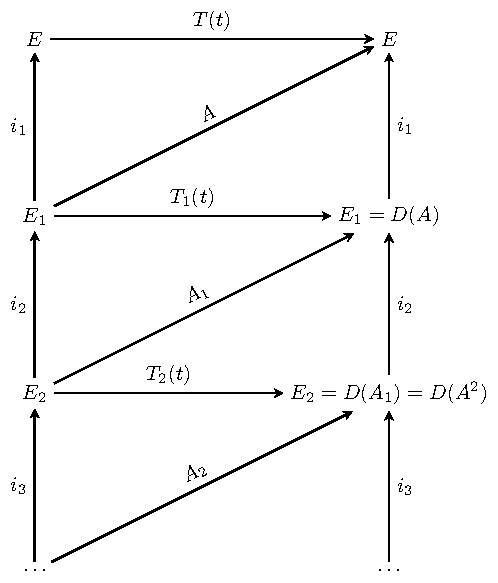
\includegraphics[width=0.8\textwidth]{./tikz-images/tikz-chap-a1-a.pdf}
\end{center}
%% --
For the translation semigroup on $L^{p}(\R)$ (see Section~\ref{subsec:a1-2.4}) the above construction leads to the usual \emph{Sobolev spaces}.
Therefore we might call $E_{n}$ the \emph{n-th Sobolev space} and $(T_{n}(t))_{t \geq 0}$ the \emph{n-th Sobolev semigroup} associated to $E$ and $(T(t))_{t \geq 0}$.
%% --
\begin{remarks*}\label{rem:a1-19.1}
%% --
\begin{enumerate}[\upshape(i), wide, labelindent=.25em]
\item
\index{resolvent}
For $\lambda \in \rho(A)$ the operator $(\lambda - A)$ and the resolvent $R(\lambda,A)$ are isomorphisms from $E_{1}$ onto $E$, \resp from $E$ onto $E_{1}$ (show that $\|\cdot\|_{1}$ and $\|\cdot\|_{\lambda}$ with $\|\cdot\|_{\lambda} \coloneq \|(\lambda - A)\cdot\|$ are equivalent).
%% --
In addition, the following diagram commutes. 
%% -- tikz
\begin{center}
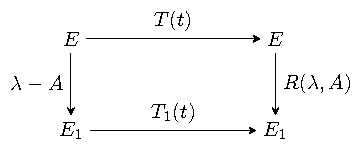
\includegraphics[width=0.6\textwidth]{./tikz-images/tikz-chap-a1-b.pdf}
\end{center}
%% 
Therefore all Sobolev semigroups $(E_{n}, T_{n}(t))_{t \geq 0}$, $n \in \N$, are equivalent.%isomorphic.

\item
For $\lambda \in \rho(A)$ and for every $f \in E$ consider the norm
%% --
\[
    \|f\|_{-1} \coloneq \|R(\lambda,A)f\|
\]
%% --
and define $E_{-1}$ as the completion of\/ $E$ for $\|\cdot\|_{-1}$.
Then $(T(t))_{t \geq 0}$ extends continuously to a strongly continuous semigroup $(T_{-1}(t))_{t \geq 0}$ on $E_{-1}$ and the diagram on the previous page can be extended to the negative integers.
\end{enumerate}
\end{remarks*}
%% --
\subsection{The \texorpdfstring{$\mathcal{F}$}{F}-Product Semigroup}\label{subsec:a1-3.7}%
%
\index{semigroup!F-product@$\mathcal{F}$-product}
\index{standard construction!fprod@$\mathcal{F}$-Product semigroup}
%% --
It is standard in functional analysis to consider a sequence of points in a certain space as a point in a new and larger space.
In particular such a method can serve to convert an approximate eigenvector of a linear operator into an eigenvector.
\index{approximate eigenvector}
Occasionally we will need such a construction and refer to Section V.1 of \textcite{schaefer:1974}. 

If we try to adapt this construction to strongly continuous semigroups we encounter the difficulty that the semigroup extended to the larger space will not remain strongly continuous.
An idea already used in Section~\ref{subsec:a1-3.4} will help to overcome this difficulty.

Let $\TT = (T(t))_{t \geq 0}$ be a strongly continuous semigroup on the Banach space $E$.
Denote by $m(E)$ the Banach space of all bounded $E$-valued sequences endowed with the norm
%% --
\[
    \|(f_{n})_{n \in \N}\| \coloneq \sup \{\|f_{n}\| \colon n \in \N\} .
\]
%% --
It is clear that every $T(t)$ extends canonically to a bounded linear operator
%% --
\[
    \widehat{T}(t)(f_{n}) \coloneq (T(t)f_{n})
\]
%% --
on $m(E)$, but the semigroup $(\widehat{T}(t))_{t \geq 0}$ is strongly continuous if and only if\/ $\TT$ has a bounded generator.
Therefore we restrict our attention to the closed, $(\widehat{T}(t))$-invariant subspace
%% --
\[
    m^{\TT}(E) \coloneq \{(f_{n}) \in m(E) \colon \lim_{t \to 0} \|T(t)f_{n}-f_{n}\| = 0 \text{ uniformly for } n \in \N\} .
\]
%% --
Then the restricted semigroup
%% --
\[
    \widehat{T}(t)(f_{n}) = (T(t)f_{n}), \quad (f_{n}) \in m^{\TT}(E)
\]
%% --
is strongly continuous and we denote its generator by $(\widehat{A},D(\widehat{A}))$.

The following lemma shows that $\widehat{A}$ is obtained canonically from $A$.
%% --
\begin{lemma*}\label{lem:a1-3.6}
For the generator $\widehat{A}$ of\/ $(\widehat{T}(t))_{t \geq 0}$ on $m^{\TT}(E)$ one has the following properties.
%% --
\begin{enumerate}[\upshape(i)]

\item 
$D(\widehat{A}) = \{(f_{n}) \in m^{\TT}(E) \colon f_{n} \in D(A) \text{ and } (Af_{n}) \in m^{\TT}(E)\}$,

\item 
$\widehat{A}(f_{n}) = (Af_{n})$ for $(f_{n}) \in D(\widehat{A})$.
\end{enumerate}
%% --
\end{lemma*}
%% --
For the proof we refer to Lemma 1.4. of \textcite{derndinger:1980}.

Now let $\mathcal{F}$ be any filter on $\N$ finer than the Fréchet filter (\ie the filter of sets with finite complement. In most cases $\mathcal{F}$ will be either the Fréchet filter or some free ultrafilter).
%% --
The space of all $\mathcal{F}$-null sequences in $m(E)$, \ie
%% --
\[
    c_{\mathcal{F}}(E) \coloneq \{(f_{n}) \in m(E) \colon \mathcal{F}\text{-}\lim\|f_{n}\| = 0\}
\]
%% --
is closed in $m(E)$ and invariant under $(\widehat{T}(t))_{t \geq 0}$. 
We call the quotient spaces
%% --
\[
    E_{\mathcal{F}} \coloneq m(E)/c_{\mathcal{F}}(E) 
    \quad \text{and} \quad 
    E_{\mathcal{F}}^{T} \coloneq m^{\TT}(E)/ (c_{\mathcal{F}}(E)\cap m^{\TT}(E))
\]
%% --
the \emph{$\mathcal{F}$-product of\/ $E$} and the \emph{$ \mathcal{F} $-product of\/ $E$ with respect to the semigroup $\TT$}, respectively.
\index{F-product@$\mathcal{F}$-product}

Thus $E_{\mathcal{F}}^{T}$ can be considered as a closed linear subspace of\/ $E_{\mathcal{F}}$. 
We have $E_{\mathcal{F}}^{T} = E_{\mathcal{F}}$ if (and only if) $\TT$ has a bounded generator.

The canonical quotient norm on $E_{\mathcal{F}}$ is given by
%% --
\[
    \|(f_{n}) + c_{\mathcal{F}}(E)\| = \mathcal{F}\text{-}\lim \sup \|f_{n}\| .
\]
%% --
We can apply Section~\ref{subsec:a1-3.4} in order to define the \emph{$\mathcal{F}$-product semigroup} $(T_{\mathcal{F}}(t))_{t \geq 0}$ on $E_{\mathcal{F}}^{T}$ by
%% --
\[
    T_{\mathcal{F}}(t)((f_{n}) + c_{\mathcal{F}}(E)) \coloneq (T(t)f_{n}) 
    	+ ( c_{\mathcal{F}}(E)\cap m^{\TT}(E) ) .
\]
%% --
Thus $T_{\mathcal{F}}(t)$ is the restriction of\/ $T(t)_{F}$ where $T(t)_{F}$ denotes the canonical extension of\/ $T(t)$ to the $\mathcal{F}$-product $E_{\mathcal{F}}$. 
But note that $(T(t)_{F})_{t \geq 0}$ is not strongly continuous unless $\TT$ has a bounded generator.

With the canonical injection $j \colon f \mapsto (f,f,f,\ldots) + c_{\mathcal{F}}(E)$ from $E$ into 
$E_{\mathcal{F}}^{T}$ the operators $T_{\mathcal{F}}(t)$ are extensions of\/ $T(t)$ satisfying $\|T_{\mathcal{F}}(t)\| = \|T(t)\|$. 
The basic facts about the generator $(A_{\mathcal{F}},D(A_{\mathcal{F}}))$ of\/ $(T_{\mathcal{F}}(t))_{t \geq 0}$ follow from Section~\ref{subsec:a1-3.3} and are collected in the following proposition.
%% --
\begin{proposition*}\label{prop:a1-3.6}
For the generator $(A_{\mathcal{F}},D(A_{\mathcal{F}}))$ of the $\mathcal{F}$-product semigroup the following holds.
%% --
\begin{enumerate}[\upshape(i)]
\item 
$D(A_{\mathcal{F}}) = \{(f_{n}) + c_{\mathcal{F}}(E) \colon f_{n} \in D(A); (f_{n}), (Af_{n}) \in m^{\TT}(E)\}$,

\item 
$A_{\mathcal{F}}((f_{n}) + c_{\mathcal{F}}(E)) = (Af_{n}) + c_{\mathcal{F}}(E)$.

\end{enumerate}
\end{proposition*}
%% --
In case $A$ is a bounded operator then $D(A_{\mathcal{F}}) = E_{\mathcal{F}}^{T} = E_{\mathcal{F}}$ and $A_{\mathcal{F}}$ is the canonical extension of\/ $A$ to $E_{\mathcal{F}}$.

We will show in Section~\ref{subsec:a3-4.5} that the above construction preserves and even improves many spectral properties of the semigroup and its generator.
%% --
\subsection{The Tensor Product Semigroup}\label{subsec:a1-3.8}%
\index{standard construction!tensor product semigroup}
\index{semigroup!tensor product semigroup}
%% --
Real- or complex-valued functions of two variables $x$, $y$ are often limits of functions of the form 
$\sum_{i=1}^{n} f_{i}(x)g_{i}(y)$ which, to some extent, allows one to consider the variables $x$ and $y$ separately.
Since algebraic manipulation with these latter functions is governed by the formal rules of a tensor product, it is customary to identify (for example) the function
%% --
\[
    (x,y) \mapsto f(x)g(y)
\]
%% --
with the tensor product $f \otimes g$ and to consider limits of linear combinations of such functions as elements of a completed tensor product.

To be more precise, we briefly present the most important examples for this situation.
%% --
\begin{examples*}\label{ex:a1-5.1}
%% --
\begin{enumerate}[\upshape(i), wide, labelindent=.25em]

\item
Let $(X,\Sigma,\mu)$ and $(Y,\Omega,\nu)$ be measure spaces. 
If we identify for $f_{i} \in L^{p}(\mu)$, $g_{i} \in L^{p}(\nu)$ the elements $\sum_{i=1}^{n} f_{i} \otimes g_{i}$ of the tensor product
%% --
\[
    L^{p}(\mu) \otimes L^{p}(\nu)
\]
%% --
with the (class of\/ $\mu \times \nu$-a.e.-defined) functions
%% --
\[
    (x,y) \mapsto \sum_{i=1}^{n} f_{i}(x)g_{i}(y) ,
\]
%% --
then $L^{p}(\mu) \otimes L^{p}(\nu)$ becomes a dense subspace of\/ $L^{p}(X\times Y,\Sigma\times\Omega,\mu\times\nu)$ for $1 \leq p < \infty$.

\item
Similarly, let $X$,$Y$ be compact spaces. Then $C(X) \otimes C(Y)$ becomes a dense subspace of\/ $C(X\times Y)$ by identifying, for $f \in C(X)$ and $g \in C(Y)$, $f \otimes g$ with the function
%% --
\[
    (x,y) \mapsto f(x)g(y) .
\]
%% --
\end{enumerate}
\end{examples*}
%% --
We do not intend to go deeper into the quite sophisticated problems related to normed tensor products of general Banach spaces, but will rather confine ourselves to the discussion of certain special cases.
These will always be related to one of the following standard methods to define a norm on the tensor product of two Banach spaces $E$, $F$.

Let $u \coloneq \sum_{i=1}^{n} f_{i} \otimes g_{i}$ be an element of\/ $E \otimes F$. 
Then
%% --
\begin{enumerate}[--,labelindent=.25em]

\item
$\|u\|_{\pi} \coloneq \inf\{\sum_{j=1}^{m} \|h_{j}\| \|k_{j}\| \colon u = \sum_{j=1}^{m}h_{j} \otimes k_{j}, h_{j} \in E, k_{j} \in F\}$ defines the \emph{greatest cross norm $\pi$} on $E \otimes F$.

\item
$\|u\|_{\epsilon} \coloneq \sup\{\langle u,\phi \otimes \psi\rangle \colon \phi \in E', \psi \in F', \|\phi\|, \|\psi\| \leq 1\}$ defines the 
\emph{least cross norm $\epsilon$} on $E \times F$. 
Here, $\langle u,\phi \otimes \psi\rangle$ denotes the canonical bilinear form on $(E \otimes F) \times (E' \otimes F')$, \ie $\langle\sum_{i=1}^{n} f_{i} \otimes g_{i},\phi \otimes \psi\rangle = \sum_{i=1}^{n} \langle f_{i},\phi\rangle\langle g_{i},\psi\rangle$.

\item
If\/ $E$ and $F$ are Hilbert spaces, $\|u\|_{h} = (u|u)_{h}^{1/2}$, where the scalar product $(\cdot|\cdot)_{h}$ is defined as above, defines the \emph{Hilbert norm $h$} on $E \otimes F$.
\end{enumerate}
%% --
In the following we write $E \otimes_{\alpha} F$ for the tensor product of\/ $E$ and $F$ endowed---if applicable---with one of the norms $\pi$, $\epsilon$, $h$ just defined.
In each case one has $\|f \otimes g\| = \|f\| \|g\|$ for $f \in E$, $g \in F$.

By $E \widetilde{\otimes}_{\alpha} F$ we mean the completion of\/ $E \otimes_{\alpha} F$. 
Moreover we recall how examples (i) and (ii) above fit into this pattern.
%%% --
%\[
%    L^{1}(\mu \otimes \nu) = L^{1}(\mu) \widetilde{\otimes}_{\pi} L^{1}(\nu), 
%    \quad 
%    C(X \times Y) = C(X) \widetilde{\otimes}_{\epsilon} C(Y) , 
%\]
%\[
%	L^{2}(\mu \otimes \nu) = L^{2}(\mu) \widetilde{\otimes}_{h} L^{2}(\nu) .
%\]
%%% --
\begin{align*}
    L^{1}(\mu \otimes \nu) &= L^{1}(\mu) \widetilde{\otimes}_{\pi} L^{1}(\nu), \\
    C(X \times Y)          &= C(X) \widetilde{\otimes}_{\epsilon} C(Y),          \\
    L^{2}(\mu \otimes \nu) &= L^{2}(\mu) \widetilde{\otimes}_{h} L^{2}(\nu).
\end{align*}
%% --
Finally, we point out that for any $S \in \LE$, $T \in \L{F} $, the mapping
%% --
\[
    \sum_{i=1}^{n}f_{i} \otimes g_{i} \mapsto \sum_{i=1}^{n}Sf_{i} \otimes Tg_{i}
\]
%% --
defined on $E \otimes F$ is linear and continuous on $E \otimes_{\alpha} F$, hence has a continuous extension to $ E \widetilde{\otimes}_{\alpha} F$. 
This operator, as well as its continuous extension, will be denoted by $S \otimes T$ and satisfies $\|S \otimes T\| = \|S\| \|T\|$. 
The notation $A \otimes B$ will also be used in the obvious way if\/ $A$ and $B$ are not necessarily bounded operators on $E$ and $F$. 
We are now ready to consider semigroups induced on the tensor product.
%% --
%\begin{proposition*}\label{prop:a1-3.7}
%Let $(S(t))_{t\geq 0}$ and $(T(t))_{t\geq 0}$ be strongly continuous semigroups on Banach spaces $E$, $F$, and let $A$, $B$ be their generators. 
%Then the family $(S(t) \otimes T(t))_{t\geq 0}$ is a strongly continuous semigroup on 
%$ E \widetilde{\otimes}_{\alpha} F $.
%The closure of\/ $A \otimes \Id + \Id \otimes B$, defined on the core $D(A) \otimes D(B)$, is its generator.
%\end{proposition*}
%% --
\begin{proposition*}\label{prop:a1-3.7}
Let $(S(t))_{t\geq 0}$ and $(T(t))_{t\geq 0}$ be strongly continuous semigroups on Banach spaces $E$ and $F$, with generators $A$ and $B$, 
respectively.
Then $\mleft(S(t) \otimes T(t)\mright)_{t\geq 0}$ is a strongly continuous 
semigroup on $E\widetilde{\otimes}_{\alpha}F$.
Its generator is the closure of $A \otimes \Id + \Id \otimes B$, with 
core $D(A) \otimes D(B)$.
\end{proposition*}
%% --
\begin{proof}
It is immediately verified that $(S(t)\otimes T(t))_{t\geq 0}$ is in fact a semigroup of operators on 
$ E \widetilde{\otimes}_{\alpha} F $. 
The strong continuity need only be verified at $t = 0$ and on elements of the form $u = f \otimes g \in E \otimes F$.

This verification being straightforward, there remains to show that the generator of\/ $(S(t)\otimes T(t))_{t\geq 0}$ is obtained as the closure of 
%
\[
	(A \otimes \Id + \Id \otimes B,D(A) \otimes D(B)) .
\]
%
To this end, let $f \in D(A)$ and $g \in D(B)$. 
Then
%% --
%\begin{align*}
%    &\lim_{h\to 0} \frac{1}{h}(T(h) \otimes S(h)(f \otimes g)-f \otimes g) \\
%    &= \lim_{h\to 0} \frac{1}{h}(T(h)f \otimes (S(h)g-g) + (T(h)f-f) \otimes g) \\
%%    &= (f \otimes Bg) + (Af \otimes g) .
%    &= f \otimes Bg + Af \otimes g.
%\end{align*}
%% --
\begin{align*}
    &\lim_{h\to 0} \frac{1}{h}\mleft(
        \mleft(T(h) \otimes S(h)\mright)(f \otimes g) - f \otimes g
      \mright) \\
    &= \lim_{h\to 0} \frac{1}{h}\mleft(
        T(h)f \otimes (S(h)g - g) + (T(h)f - f) \otimes g
      \mright) \\
    &= f \otimes Bg + Af \otimes g.
\end{align*}
%% --
Since the elements of the form $f \otimes g$, $f \in D(A)$, $g \in D(B)$, generate the linear subspace $D(A) \otimes D(B)$ of\/ $E \otimes_{\alpha} F$, this subspace belongs to the domain of the generator.
Moreover, $D(A) \otimes D(B)$ is dense in $E \widetilde{\otimes}_{\alpha} F$ and invariant under $(S(t)\otimes T(t))_{t\geq 0}$, hence it is a core of\/ $A \otimes \Id + \Id \otimes B$ by Proposition~\ref{prop:a1-1.9}\,(ii).
\end{proof}
%% -- 
\subsection{The Product of Commuting Semigroups}\label{subsec:a1-3.9}%
\index{standard construction!commuting semigroup}
%% --
Let $(S(t))_{t\geq 0}$ and $(T(t))_{t\geq 0}$ be semigroups with generators $A$ and $B$, respectively on some Banach space $E$.
It is not difficult to see that the following assertions are equivalent.
%% --
\begin{enumerate}[\upshape (a)]

\item  
$S(t)T(t) = T(t)S(t)$ for all $t \geq 0$.

\item 
$R(\mu,A)R(\mu,B) = R(\mu,B)R(\mu,A)$ for some $\mu \in \rho(A) \cap \rho(B)$.

\item 
$R(\mu,A)R(\mu,B) = R(\mu,B)R(\mu,A)$ for all $\mu \in \rho(A) \cap \rho(B)$.

\end{enumerate}
%% --
In that case $U(t) = S(t)T(t)$ $(t \geq 0)$ defines a semigroup $(U(t))_{t\geq 0}$.
Using %Proposition~\ref{prop:a1-1.9}\,(ii).
Proposition~\ref{prop:a1-1.9}\,(ii) one easily shows that $D_{0} \coloneq D(A) \cap D(B)$ is a core for its generator $C$ and $Cf = Af + Bf$ for all $f \in D_{0}$.
%% --
%\newpage
\section*{Notes}
\addcontentsline{toc}{section}{Notes}
%\sectionnopage{Notes \& References}
%\markboth{Notes and References}{Notes and References}
For more complete information on semigroup theory we refer the reader to \textcite{hillephillips:1957}, to the monographs by \textcite{davies:1980}, 
\textcite{goldstein:1985a} and \textcite{pazy:1983}, to the survey article by \textcite{kreinkhazan:1985} and to the bibliography by 
\textcite{goldstein:1985b}. 
%% --
%% -- References 
%% --
\section*{References}
\addcontentsline{toc}{section}{References}
{\RaggedRight
  \printbibliography[heading=none]
 }

%    \pagestyle{headings}
    % !TEX root = ../LN-Book-New.tex
%% -- Stand: 2026-03-14
%% -- 2026-03-21 (GG  hat Kleinigkeiten korrigiert)
%% --
%%\setcounter{section}{0}
%% --
\chapternopage{Characterization of Semigroups on Banach Spaces}\label{chap:a2}
\chaptermark{Characterization of Semigroups}
\thispagestyle{empty}%
%% --
In this chapter two different problems are treated.
%% –
\textit{%
\begin{enumerate}[\upshape (i)]
\item 
To characterize generators of strongly continuous semigroups.
\item 
To characterize various properties of strongly continuous semigroups in terms of their generators.
\end{enumerate}
}
%% –
In Section~\ref{sec:a2-1} the first problem is solved by finding conditions on the Cauchy problem associated with $A$ and also by finding conditions on the resolvent of\/ $A$.
The second problem is treated by considering a hierarchy of smoothness properties of the semigroup.

Contraction semigroups are considered in Section~\ref{sec:a2-2}.
Here, the first problem has a simple and extremely useful solution: A densely defined operator $A$ is the generator of a contraction semigroup if and only if\/ $A$ is dissipative and satisfies a range condition.

Our approach is quite general.
We not only consider contractions with respect to the norm but also with respect to \emph{half-norms}.
This will allow us to obtain results on positive contraction semigroups simultaneously by choosing a suitable half-norm (\cf Part-III, Section~\ref{sec:c2-1}).

The last section contains a surprising result: on certain Banach spaces (\eg $L^{\infty}$) only bounded operators are generators of strongly continuous semigroups.
%% --
\section{The Abstract Cauchy Problem, Special Semigroups and Perturbation} \label{sec:a2-1}%
\index{abstract Cauchy problem}
%% --
\hspace{1cm}{\Large by Wolfgang Arendt}
\vspace{.5cm}
\newline
%% --
Linear differential equations in Banach spaces are intimately connected with the theory of one-parameter semigroups.
In fact, given a closed linear operator $A$ with dense domain $D(A)$, the following statement is true (with some reservation regarding a technical detail).
%% --
\begin{quote}
\textit{The abstract Cauchy problem}
%% –
\begin{align*}
	\dot{u}(t) &= Au(t) \quad (t \geq 0) \\
	u(0) &= f 
\end{align*}
%% –
\textit{has a unique solution for every $f \in D(A)$ if and only if\/ $A$ is the generator of a strongly continuous semigroup.}
\end{quote}
%% --
This is one characterization of generators which illustrates their important role for applications.
The fundamental Hille-Yosida theorem gives a different characterization in terms of the resolvent and yields a powerful tool for actually proving that a given operator is the generator of a semigroup.

Another problem we will treat here is how diverse properties of a semigroup can be described in terms of its generator.
This is a reasonable question from the theoretical point of view (since the generator uniquely determines the semigroup).
It is of interest from the practical point of view as well: the generator is the given object, defined by the differential equation.
It is useful to dispose of conditions of the generator itself giving information on the solutions (which might not be known explicitly).
We discuss smoothness properties such as analyticity, differentiability, norm continuity and compactness of the semigroup.

A frequent method to obtain new generators out of a given one is by perturbation.
We will have a brief look at this circle of problems at the end of this section.

The results are explained and illustrated by examples.
Proofs are only given when new aspects are presented which are not yet contained in the literature, otherwise we refer to the recent monographs \textcite{davies:1980}, \textcite{goldstein:1985a}, \textcite{pazy:1983}.
%% --
\subsection{The Abstract Cauchy Problem} \label{subsec:a2-1.se1}
%% --
Let $A$ be a closed operator on a Banach space $E$ and consider the \emph{Abstract Cauchy Problem \eqref{eq:a2-acp}}
%% –
% \begin{equation*}\label{eq:a2-acp} \tag{ACP}
% \left.
% \begin{split}
%     \dot{u}(t) &= Au(t) \quad (t \geq 0) \\
%     u(0) &= f
% \end{split} 
% \right\}   
% \end{equation*}
%% –
\begin{equation*}\label{eq:a2-acp} \tag{ACP}
\left.
\begin{aligned}
    \dot{u}(t) &= Au(t) \quad (t \geq 0) \\
    u(0) &= f
\end{aligned} 
\right\}   
\end{equation*}
%% --
By a solution of \eqref{eq:a2-acp} for the initial value $f \in D(A)$ we understand a continuously differentiable function $u \colon \left[0,\infty\right) \to E$ satisfying $u(0) = f$ and $u(t) \in D(A)$ for all $t \geq 0$ such that $\dot{u}(t) = Au(t)$ for $t \geq 0$.

By Theorem~\ref{thm:a1-1.7} there exists a unique solution of \eqref{eq:a2-acp} for all initial values in the domain $D(A)$ whenever $A$ is the generator of a strongly continuous semigroup.
The converse does not hold (see Example~\ref{ex:a2-1.4} below).
However, for the operator $A_{1}$ on the Banach space $E_{1} = D(A)$ 
(see Section~\ref{subsec:a1-3.6}) with domain 
$D(A_{1}) = D(A^{2})$ given by $A_{1}f = Af$ $(f \in D(A_{1}))$ the following holds.
%% –
\begin{theorem}\label{thm:a2-1.1}
The following assertions are equivalent.
%% --
\begin{enumerate}[\upshape (a)]

\item \label{thm:a2-1.1-1}
For every $f \in D(A)$ there exists a unique solution of \eqref{eq:a2-acp}.

\item \label{thm:a2-1.1-2}
$A_{1}$ is the generator of a strongly continuous semigroup.
\end{enumerate}
%% --
\end{theorem}
%% –
\begin{proof} (a) $\implies$ (b):   
Assume that (a) holds, \ie for every $f \in D(A)$ there exists a unique solution $u(\cdot,f) \in C^{1}(\left[0,\infty\right),E)$ of \eqref{eq:a2-acp}.
For $f \in E_{1}$ define 
%%
\[
T_{1}(t)f \coloneq u(t,f) .
\]
%%
By the uniqueness of the solutions it follows that $T_{1}(t)$ is a linear operator on $E_{1}$ and $T_{1}(s+t) = T_{1}(s)T_{1}(t)$.
Moreover, since $u(\cdot,f) \in C^{1}$, it follows that $t \mapsto T_{1}(t)f$ is continuous from $[0,\infty)$ into $E_{1}$.
We show that $T_{1}(t)$ is a continuous operator for all $t > 0$.

Let $t > 0$ and consider the mapping $\eta \colon E_{1} \to C([0,t],E_{1})$ given by 
%% --
\[
    \eta(f) = T_{1}(\cdot)f = u(\cdot,f) .
\]
%% --
We show that $\eta$ has a closed graph.

In fact, let $f_{n} \to f$ in $E_{1}$ and $\eta(f_{n}) = u(\cdot,f_{n}) \to v$ in $C([0,t],E_{1})$.
Then 
%% --
\[
u(s,f_{n}) = f_{n} + \int_{0}^{s} Au(r,f_{n}) \dr .
\]
%% --
Letting $n \to \infty$ we obtain $v(s) = f + \int_{0}^{s} Av(r) \dr$ for $0 \leq s \leq t$.

Let 
\[
\tilde{v}(s) = 
\begin{cases}
    T_{1}(s-t)v(t)      & \text{for $s > t$,}\\
    v(s) & \text{for $0 \leq s \leq t$.}
\end{cases}
\]
%% --
Then $\tilde{v}$ is a solution of \eqref{eq:a2-acp}.
It follows that $\tilde{v}(s) = T_{1}(s)f$ for all $s \geq 0$.
Hence $v = \eta(f)$.

We have shown that $\eta$ has a closed graph and so $\eta$ is continuous.
This implies the continuity of\/ $T_{1}(t)$.
It remains to show that $A_{1}$ is the generator of\/ $(T_{1}(t))_{t \geq 0}$.

We first show that for $f \in D(A^{2})$ one has
%% –
\begin{equation}\label{eq:a2-1.1}
AT_{1}(t)f = T_{1}(t)Af.
\end{equation}
%% –
In fact, let $v(t) = f + \int_{0}^{t} u(s,Af) \ds$.
Then 
%% --
\[
\dot{v}(t) = u(t,Af) = Af + \int_{0}^{t} Au(s,Af) \ds = A(f + \int_{0}^{t} u(s,Af) \ds) = Av(t). 
\]
%% --
Since $v(0) = f$, it follows that $v(t) = u(t,f)$.
Hence 
%
\[
	Au(t,f) = Av(t) = \dot{v}(t) = u(t,Af) .
\]
%
This is Eq.~\myeqpageref{eq:a2-1.1}.
%%--
Now denote by $B$ the generator of\/ $(T_{1}(t))_{t \geq 0}$.
For $f \in D(A^{2})$, we have
%% –
\[
    \lim_{t \to 0} \frac{1}{t}\mleft( T_{1}(t)f - f \mright) = Af
\]
%% –
and by Eq.~\myeqpageref{eq:a2-1.1},
%% –
\[
    \lim_{t \to 0} A\frac{1}{t} \mleft( T_{1}(t)f - f \mright) = 
    \lim_{t \to 0} \frac{1}{t} \mleft( T_{1}(t)Af - Af \mright)
    = A^{2}f
\]
%% –
in the norm of\/ $E$.
Hence 
% --
\[ 
\lim_{t \to 0} \frac{1}{t} \mleft( T_{1}(t)f - f \mright) = Af
\]
%% --
in the norm of\/ $E_{1}$.
This shows that $A_{1} \subseteq B$.

In order to show the converse, let $f \in D(B)$.
Then 
% --
\[ 
\lim_{t \to 0} \frac{1}{t} \mleft( T_{1}(t)f - f \mright)
\]
%% --
exists in the norm of\/ $E$.
Since  
% --
\[ 
\lim_{t \to 0} \frac{1}{t} \mleft( T_{1}(t)f - f \mright)
= Af 
\]
%% --$ 
in the norm of $E$, it follows that $Af \in D(A)$, since $A$ is closed.
Thus 
%% --
\[
f \in D(A^{2}) = D(A_{1})
\]
%% --
and we have shown that $B = A_{1}$.

(b)  $\implies$ (a):  
Assume that $A_{1}$ is the generator of a strongly continuous semigroup $(T_{1}(t))_{t \geq 0}$ on $E_{1}$.
Let $f \in D(A)$ and set 
%% -
\[
u(t) = T_{1}(t)f.
\]
%% --
Then $u \in C(\left[0,\infty\right),E)$ and $Au(\cdot) \in C([0,\infty),E)$.
Moreover, 
%% --
\[
\int_{0}^{t} u(s) \ds = \int_{0}^{t} T_{1}(s) f   \ds \in D(A_{1}) = D(A^{2})
\]
%% --
and 
%% --
\[
A\int_{0}^{t} u(s) \ds = u(t) - u(0) = u(t) - f
\]
%% --
(by Eq.~\myeqpageref{eq:a1-1.3}).
Consequently, 
%% --
\[
    u(t) = f + \int_{0}^{t} Au(s) \ds .
\]
%% --
Hence $u \in C^{1}(\left[0,\infty  \right),E)$ and $\dot{u}(t) = Au(t)$.
Thus $u$ is a solution of \eqref{eq:a2-acp} and we have shown existence.

In order to show uniqueness, assume that $u$ is a solution of \eqref{eq:a2-acp} with initial value $0$.
We have to show that $u \equiv 0$.

Let $v(t) = \int_{0}^{t} u(s)\ds$.
Then $v(t) \in D(A)$ and
%% --
\[
    Av(t) = \int_{0}^{t} Au(s)\ds 
          = \int_{0}^{t} \dot{u}(s)\ds 
          = u(t) \in D(A),
\]
%% --
hence $v(t) \in D(A^{2})$ for all $t \geq 0$.
Moreover, $\dot{v}(t) = u(t) = Av(t)$ and
%% --
\[
    \frac{\diff{}}{\dt}Av(t) = Au(t) = A_{1}\dot{v}(t) = A^{2}v(t).
\]
%% --
Thus $v \in C^{1}([0,\infty), E_{1})$ satisfies $\dot{v}(t) = A_{1}v(t)$.
Since $v(0) = 0$, it follows that $v \equiv 0$, and hence $u \equiv 0$.
\end{proof}
%% --
If \eqref{eq:a2-acp} has a unique solution for every initial value in $D(A)$, then $A$ is the generator of a strongly continuous semigroup only if some additional assumptions on the solutions (continuous dependence on the initial value) or on $A$ $(\rho(A) \neq \emptyset)$ are made.
%% –
\begin{corollary}\label{cor:a2-1.2}
Let $A$ be a closed operator.
Consider the following existence and uniqueness condition.
%%% –
%\begin{empheq}[left=(EU)\quad\empheqlbrace]{align*}
%	&\text{For every $f \in D(A)$ there exists a unique solution} \\
% 	&\text{$u(\cdot,f) \in C^{1}([0,\infty),E)$ of the Cauchy problem associated with $A$ }\\ 
%	&\text{having the initial value $u(0,f) = f$.}
%\end{empheq}
%%% --
%% --
\begin{empheq}[left={(EU)\quad\empheqlbrace\,}]{align*}
    &\text{For every $f \in D(A)$ there exists a unique solution} \\
    &\text{$u(\cdot,f) \in C^{1}([0,\infty),E)$ of the Cauchy problem associated with $A$} \\
    &\text{having the initial value $u(0,f) = f$.}
\end{empheq}
%% --
The following assertions are equivalent.
%% --
\begin{enumerate}[\upshape (a)]

\item\label{cor:a2-1.2-1}
$A$ is the generator of a strongly continuous semigroup.

\item\label{cor:a2-1.2-2}
$A$ satisfies (EU) and $\rho(A) \neq \emptyset$.

\item\label{cor:a2-1.2-3}
$A$ satisfies (EU) and for every $\mu \in \R$ there exists $\lambda > \mu$ such that $(\lambda-A)D(A) = E$.
\item\label{cor:a2-1.2-4}
$A$ satisfies (EU), has dense domain and for every sequence $(f_{n})$ in $D(A)$ satisfying $\lim_{n \to \infty}f_{n} = 0$ one has $\lim_{n \to \infty}u(t,f_{n}) = 0$ uniformly in $t \in [0,1]$.

\end{enumerate}
\end{corollary}
%% –
\begin{proof}
It is clear that (a) implies the remaining assertions.
So assume that $A$ satisfies (EU).
Then by Theorem~\ref{thm:a2-1.1}, $A_{1}$ is a generator.
If there exists $\lambda \in \rho(A)$, then $(\lambda-A)$ is an isomorphism from $E_{1}$ onto $E$ and $A$ is similar to $A_{1}$ via this isomorphism since 
%% --
\[
D(A_{1}) = \{(\lambda-A)^{-1}f \colon f \in D(A)\}
\]
%% --
and 
%
\[
	Af = (\lambda-A)A_{1}(\lambda-A)^{-1}f
	\quad \text{for all} \quad f \in D(A)
\]
%
(see Section~\ref{subsec:a1-3.1}).
Thus $A$ is a generator on $E$ and we have shown that (b) implies (a).   

If (c)  holds, then there exists $\lambda > s(A_{1})$ such that $(\lambda-A)D(A) = E$.
We show that $(\lambda-A)$ is injective.
Then $\lambda \in \rho(A)$ since $A$ is closed.
Assume that $\lambda f = Af$ for some $f \in D(A)$.
Then $f \in D(A^{2}) = D(A_{1})$, and so $f = 0$ since $\lambda \in \rho(A_{1})$.
This proves that (c) implies (b).  

It remains to show that (d)  implies (a). 
Assertion (d) (and the semigroup property) implies that for all $ t \geq 0 $ there exist bounded operators $ T(t) \in \LE $ such that 
%
\[
	u(t,f) = T(t)f 
	\quad \text{if} \quad 
	f \in D(A) .
\]
%
Moreover, 
%
\[
	\sup_{0 \leq t \leq 1} \|T(t)\| < \infty .
\]
%
It follows that $ T(\cdot)f $ is strongly continuous for all $ f \in E $ (since it is so for $ f \in D(A) $ and $ D(A) $ is dense).

Let $ t > 1 $.
There exist unique $ n \in \N $ and $ s \in [0,1) $ such that $ t = n + s $.
Let 
%
\[
	T(t) \coloneq T(1)^{n} \cdot T(s) .
\]
%
From the uniqueness of the solutions it follows that $ T(t)f = u(t,f) $ for all $ t \geq 0 $ as well as $ T(t+s)f = T(s)T(t)f $ for all $ f \in D(A) $ and $ s$, $t \geq 0 $.
Thus $ T $ is a semigroup.

Denote by $ B $ its generator.
It follows from the definition that $ A \subseteq B $.
Moreover, $ D(A) $ is invariant under the semigroup.
So by Proposition~\ref{prop:a1-1.9}\,(ii) $ D(A) $ is a core of\/ $ B $.
Since $ A $ is closed this implies that $ A = B $.
\end{proof}
%% --
\begin{remark}\label{rem:a2-1.3}
It is surprising that from conditions~\ref{cor:a2-1.2-2}   and~\ref{cor:a2-1.2-3}   in the corollary it follows automatically that $ D(A) $ is dense.
On the other hand, this condition cannot be omitted in~\ref{cor:a2-1.2-4}.   
In fact, consider any generator $ \tilde{A} $ and its restriction $ A $ with domain $ D(A) = \{0\} $.
Then $ A $ satisfies the remaining conditions in~\ref{cor:a2-1.2-4} but is not a generator (if\/ $ \dim E > 0 $).
\end{remark}
%% --
\begin{example}\label{ex:a2-1.4}
We give a densely defined closed operator $ A $ such that there exists a unique solution of \eqref{eq:a2-acp} for all initial values in $ D(A) $, but $ A $ is not a generator.

Let $ B $ be a densely defined unbounded closed operator on a Banach space $ F $.
Consider $ E = F \oplus F $ and $ A $ on $ E $ given by
%% --
\[
    A \coloneq \begin{pmatrix} 0 & B \\ 0 & 0 \end{pmatrix}
\]
%% --
with domain $ F \times D(B) $.

Then $ D(A^{2}) = \{(f,g) \in F \times D(B) \colon Bg \in F\} = D(A) $ and so $ A_{1} \in \L{E_{1}} $.
In particular, $ A_{1} $ is a generator while
$ A $ is not. For instance
condition~\ref{cor:a2-1.2-2}   in Corollary~\ref{cor:a2-1.2}   does not hold since, for each $ \lambda \in \C $
%% --
\[
    (\lambda-A)D(A) = \{(\lambda f-Bg,\lambda g) \colon f \in F, g \in D(B)\} \subseteq F \times D(B) \neq F \times F = E ,
\]
%% --
so $ \rho(A) = \emptyset $.

As a further illustration, we note that the solution of the corresponding abstract Cauchy problem for the initial value $ (f,g) \in F \times D(B) $ is given by 
%$ 
\[
u(t) = (f + tBg,g) .
\] 
%$

Since $ B $ is unbounded, condition~\ref{cor:a2-1.2-4}  of Corollary~\ref{cor:a2-1.2}  is clearly violated.
\end{example}
%% --
\begin{remark}\label{rem:a2-1.5} 
It may happen that a generator $A$ can be extended to a closed operator $B$.
Then one can consider the abstract Cauchy problem~\eqref{eq:a2-acp} associated with $B$.
It also has a solution for every initial value in $D(B)$, but none of the solutions is unique unless $A = B$.

In fact, denote by $(T(t))_{t \geq 0}$ the semigroup generated by $A$.
Let $f \in D(B)$.
Let $\lambda > \omega_{0}(A)$.
Then there exists $g \in D(A)$ such that $(\lambda-B)f = (\lambda-A)g$.
Let $h = f - g$.
Then $h \in \ker(\lambda-B)$.
Define $u$ by 
%
\[
	u(t) = \eu^{\lambda t}h + T(t)g .
\]
%
Then $u$ is a solution of~\eqref{eq:a2-acp} for $B$ with initial value $f$.
It follows from Corollary~\ref{cor:a2-1.2} that there exists a non-trivial solution for the initial value $0$.
\end{remark}
%% --
\subsection{One-parameter Groups} \label{subsec:a2-1.se2}%
%
Generators of one-parameter groups can be characterized similarly by existence and uniqueness of the solutions of the associated Cauchy problem.
However, here the assumption of continuous dependence on the initial values can be relaxed (in fact, one has no longer to assume that the continuous dependence is uniform in $t$).
%% --
%\stepcounter{theorem}
%\begin{theorem}\label{thm:a2-1.6}
%Let $A$ be a closed densely defined operator.
%The following assertions are equivalent.
%%% –
%\begin{enumerate}[\upshape (a)]
%\item \label{thm:a2-1.6.1}
%$A$ is generator of a strongly continuous one-parameter group.
%\item  \label{thm:a2-1.6.2}
%For every $f \in D(A)$ there exists a unique function $u(\cdot,f) \in C^{1}(\R)$ satisfying $u(t,f) \in D(A)$ for all $t \in \R$ and $u(0,f) = f$ such that $\frac{\diff{}}{\dt}u = Au(t,f)$, \\
%and if\/ $f_{n} \in D(A)$ such that $\lim_{n \to \infty} f_{n} = 0$, then $\lim_{n \to \infty} u(t,f_{n}) = 0$ for all $t \in \R$.
%\end{enumerate}
%\end{theorem}
%% --
\begin{theorem}\label{thm:a2-1.6}
Let $A$ be a closed densely defined operator.
The following assertions are equivalent.
%% --
\begin{enumerate}[\upshape (a)]
\item \label{thm:a2-1.6.1}
$A$ is the generator of a strongly continuous one-parameter group.
%% --
\item \label{thm:a2-1.6.2}
For every $f \in D(A)$ there exists a unique function
$u(\cdot,f) \in C^{1}(\R)$ with $u(t,f) \in D(A)$ for all $t \in \R$,
$u(0,f) = f$, and
%% --
\[
    \frac{\diff{}}{\dt}\,u(t,f) = Au(t,f) \qquad (t \in \R).
\]
%% --
Moreover, if\/ $f_n \in D(A)$ with $\lim_{n \to \infty} f_n = 0$,
then $\lim_{n \to \infty} u(t,f_n) = 0$ for all $t \in \R$.
\end{enumerate}
\end{theorem}
%% –
\begin{proof}
It is clear that~\ref{thm:a2-1.6.1} implies~\ref{thm:a2-1.6.2}. 
If~\ref{thm:a2-1.6.2}   holds then there exist operators $T(t) \in \mathcal{L}(E)$ such that 
%
\[
	u(t,f) = T(t)f \quad (t \in \R, f \in D(A)) .
\]
%
It follows from the uniqueness of the solutions that $T(t+s) = T(t)T(s)$ $(s,t \in \R)$.

Let $f \in E$. 
There exist $(f_{n}) \in D(A)$ such that $\lim_{n \to \infty} f_{n} = f$.
Then $\lim_{n \to \infty} T(t)f_{n} = T(t)f$ for all $t \in \R$.
Since $T(\cdot)f_{n}$ is continuous, it follows that $T(\cdot)f$ is measurable.
Hence by \textcite[10.2.1]{hillephillips:1957} 
%
\[
	\sup_{t \in J}\|T(t)\| < \infty
\]
%
for every compact interval $J \subseteq (0,\infty)$.

By the group property this implies that $T(\cdot)$ is norm bounded on bounded subsets of\/ $\R$ and
$T(\cdot)f$ is continuous if\/ $f \in D(A)$.
Since $D(A)$ is dense, this implies the strong continuity of\/ $(T(t))_{t \in \R}$.
As in the proof of Corollary~\ref{cor:a2-1.2} one shows that $A$ is its generator.
\end{proof}
%%
\subsection{The Hille-Yosida Theorem} \label{subsec:a2-1.se3}%
\index{Hille-Yosida theorem|(}
\index{resolvent|(}
%% --
Given an operator $A$, frequently it is easier to obtain information about its resolvent than to solve the Cauchy problem.
Therefore the following theorem is central in the theory of one-parameter semigroups.
%% --
\begin{theorem}[Hille-Yosida]\label{thm:a2-1.7}
Let $A$ be an operator on a Banach space $E$.
The following conditions are equivalent.
%% –
\begin{enumerate}[\upshape (a)]
\item \label{thm:a2-1.7.1}
$A$ is the generator of a strongly continuous semigroup.
\item \label{thm:a2-1.7.2}
The domain  $D(A)$ of\/ $A$ is dense in $E$ and there exist $w$, $M \in \R$ such that $(w,\infty) \subseteq \rho(A)$ and
%% –
\[
    \| {(\lambda - w)^{n}} (\lambda-A)^{-n}\| \leq M 
\]
%% –
for all $\lambda > w$ and $n \in \N$.
\end{enumerate}
\end{theorem}
%% –
In general it is not easy to give an estimate for the powers of the resolvent in order to apply Theorem~\ref{thm:a2-1.7}. 
However, there is an important case when it suffices to consider merely the resolvent.
%% --
\begin{corollary}\label{cor:a2-1.8}
For an operator $A$ on a Banach space $E$ the following assertions are equivalent.
%% –
\begin{enumerate}[\upshape (a)]
\item \label{cor:a2-1.8.1}
$A$ is the generator of a strongly continuous contraction semigroup.
\item \label{cor:a2-1.8.2}
$A$ is densely defined, $(0,\infty) \subseteq \rho(A)$ and $\|\lambda R(\lambda,A)\| \leq 1$ for all $\lambda > 0$.
\end{enumerate}
\end{corollary}
%% –
The difficult part in the proof of Theorem~\ref{thm:a2-1.7}   is to show that~\ref{thm:a2-1.7.2}   implies~\ref{thm:a2-1.7.1}. 
One has to construct the semigroup out of the resolvent.
We mention two formulas which can be used for the proof.
%% --
\begin{proposition}\label{prop:a2-1.9}
Let $A$ be the generator of a strongly continuous semigroup
$(T(t))_{t \geq 0}$.
For $\lambda > 0$ let 
\[
A(\lambda) = \lambda^{2} R(\lambda,A)-\lambda \Id  =\lambda A R(\lambda,A).
\]
%% --
Then
%% –
\begin{equation}\label{eq:a2-1.2}
    T(t)f = \lim_{\lambda \to \infty} \eu^{tA(\lambda)}f
\end{equation}
%% –
for all $f \in E$ and $t \geq 0$.
\end{proposition}
%% –
Yosida's proof consists in showing that the limit in Eq.~\myeqpageref{eq:a2-1.2} exists under the hypothesis~\ref{thm:a2-1.7.2} of Theorem~\ref{thm:a2-1.7}  
(see \textcite{davies:1980}, \textcite{goldstein:1985a} or \textcite{pazy:1983}).

The proof of Hille (see \textcite{kato:1976}) is inspired by the following formula.
\index{Hille-Yosida theorem|)}
%%
\begin{proposition}\label{prop:a2-1.10}
Let $A$ be the generator of a strongly continuous semigroup $(T(t))_{t \geq 0}$.
Then
%% –
\begin{equation}\label{eq:a2-1.3}
    T(t)f = \lim_{n \to \infty} (\Id - t/nA)^{-n} f = \lim_{n \to \infty} (n/t \cdot R(n/t,A))^{n} f
\end{equation}
%% –
for all $f \in E$ and $t \geq 0$.
\end{proposition}
%% --
\subsection{Holomorphic Semigroups} \label{subsec:a2-1.se4}%
\index{semigroup!holomorphic semigroup|(}
%% --
We now describe a hierarchy of smoothness conditions on the semigroup, starting with the most restrictive class; namely, holomorphic semigroups.
The generators of these semigroups can be characterized by a particularly simple condition.

For $\alpha \in (0,\pi]$ we define the sector $S(\alpha)$ in the complex plane by
%% –
\[
    S(\alpha) = \{r\eu^{\im\theta} \colon r > 0, \theta \in (-\alpha,\alpha)\} .
\]
%% –
%% --
\begin{definition}\label{def:a2-1.11}
Let $\alpha \in (0,\pi/2]$.
A strongly continuous semigroup $(T(t))_{t \geq 0}$ is called a \emph{bounded holomorphic semigroup of angle $\alpha$} if\/ $T(\cdot)$ on $(0,\infty)$ is the restriction of a holomorphic function
%% –
\[
    T \colon S(\alpha) \to \LE
\]
%% –
satisfying
%% –
\begin{enumerate}[\upshape(i), wide, labelindent=.25em]

\item
$T(z)T(z') = T(z+z') \quad (z \text{ and } z' \in S(\alpha))$,

\item
For each  $ \alpha_{1} \in (0,\alpha) $  the set   
$ \{ T(z) \colon z \in S(\alpha_{1}) \} $
is uniformly bounded, and  
$\lim_{n \to \infty} T(z_{n})f = f$ 
for every null-sequence  $(z_{n})$ 
in  $ S( \alpha_{1} ) $  and every   $f \in E$.

\end{enumerate}
%% --
%\begin{equation}\label{eq:a2-1.4}
%    $T(z)T(z') = T(z+z') \quad (z,z' \in S(\alpha))$,
%\end{equation}
%%% –
%\begin{equation}\label{eq:a2-1.5}
%\begin{split}
%    \text{For each } \alpha_{1} \in (0,\alpha) \text{ the set } \{T(z) \colon z \in S(\alpha_{1})\} \text{ is uniformly bounded, and }\\
%%% –
%\lim_{n \to \infty} T(z_{n})f = f \text{ for every null-sequence } (z_{n}) \text{ in } S(\alpha_{1}) \\ \text{ and every } f \in E.
%\end{split}     
%\end{equation}
%% --
\end{definition}
%% --
\begin{remark*}\label{rem:a2-1.5-kgk}
A function $T \colon S(\alpha) \to \LE$ is holomorphic with respect to the operator norm if and only if it is strongly holomorphic if and only if it is weakly holomorphic (\textcite[V.3]{yosida:1965}).
\end{remark*}
%% --
\begin{theorem}\label{thm:a2-1.12}
Let $A$ be a densely defined operator on a Banach space $E$ and $\alpha \in (0,\pi/2]$.
Then $A$ is the generator of a bounded holomorphic semigroup of angle $\alpha$ if and only if 
%% –
\[
S(\alpha + \pi/2) \subseteq \rho(A)
\]
%%-
and for every $\alpha_{1} \in (0,\alpha)$ there exists a constant $M$ such that
%% –
\begin{equation}\label{eq:a2-1.6}
    \|R(\lambda,A)\| \leq M/|\lambda| \quad (\lambda \in S(\alpha_{1} + \pi/2)). 
\end{equation}
%% –
\end{theorem}
For the proof we refer to \textcite{davies:1980}, for example.
%% --
\begin{remark*}\label{rem:a2-1.6-kgk}
Let $A$ be the generator of a bounded holomorphic semigroup $(T(t))_{t \geq 0}$ 
of angle $\alpha$, and let $z_{0} \in S(\alpha)$.
Then $z_{0}A$ generates a bounded semigroup 
$(S(t))_{t \geq 0}$ given by $S(t) = T(z_{0}t)$  $(t \geq 0)$ (where again we denote by $T(z)$ the holomorphic extension of\/ $(T(t))_{t \geq 0}$ on $S(\alpha)$).
\end{remark*}
%% --
As an application of Theorem~\ref{thm:a2-1.12}  we prove the following.
%% --
\begin{corollary}\label{cor:a2-1.13}
Let $A$ be the generator of a bounded group.
Then $A^{2}$ generates a bounded holomorphic semigroup of angle $\pi/2$.
\end{corollary}
%% –
\begin{proof}
Let $0 < \alpha_{1} < \pi/2$ and $\lambda \in S(\alpha_{1} + \pi/2)$.
There exist $r > 0$ and $\beta \in (-\beta_{1},\beta_{1})$,
where $\beta_{1} \coloneq (\alpha_{1} + \pi/2)/2$
such that $\lambda = r^{2}\eu^{\iu 2\beta}$.
Then 
\[
(\lambda - A^{2}) = (r\eu^{\iu\beta} - A)(r\eu^{\iu\beta} + A) \, .
\] 
It follows that $\lambda \in \rho(A^{2})$ and 
%%--
\begin{equation}\label{eq:a2-1.7}
    R(\lambda,A^{2}) = R(r\eu^{\im\beta},A)R(r\eu^{\im\beta},-A) \, .
\end{equation}
%% –
Since $A$ generates a bounded group, there exists a constant $N \geq 0$ such that 
%
\[
	\|R(\mu,A)\| \leq N\Re(\mu)^{-1} \quad \text{and} \quad \|R(\mu,-A)\| \leq N \Re(\mu)^{-1} 
\]
%
for all $\mu \in S(\pi/2)$.
Consequently, 
%
\begin{equation*}
	\|R(\lambda,A^{2})\| \leq \frac{N^{2}}{r^{2} (\cos\beta)^{2}} 
		\leq \frac{1}{r^{2}}\mleft( \frac{N}{\cos\beta} \mright)^{2} = M\,|\lambda|^{-1} .
\qedhere
\end{equation*}
%
\end{proof}
%%
The corollary will be extended below.
We first consider an example.
%% --
\begin{example*}[The Laplacian on $E = C_{0}(\R^{n})$ or $L^{p}(\R^{n})$ $(1 \leq p < \infty)$]\label{ex:a2-1.13-kgk} 
\index{operator!Laplacian}
%% --
\begin{enumerate}[\upshape (i), wide, labelindent=.25em]
%% --
\item \label{ex:a2-1.13-kgk-1}
Let $n = 1$.
Then $(U(t)f)(x) = f(x+t)$ $(x \in \R)$ defines an isometric group on $E$.
Its generator $A$ is given by 
%%
\[
Af = f'
\]  
%%
with
%%
\[
D(A) = \{f \in C^{1}(\R) \cap C_{0}(\R) \colon f' \in C_{0}(\R)\}
\quad \text{ in the case } E = C_{0}(\R)
\]
%%
and
%%
\[
D(A) = \{f \in E \cap AC(\R) \colon f' \in E\} \quad \text{in the case } E = L^{p}
\] 
%%
(see Section~\ref{subsec:a1-2.4}).
Thus $A^{2}$ generates a bounded holomorphic semigroup by Corollary~\ref{cor:a2-1.13}. 
%%-
\item \label{ex:a2-1.13-kgk-2}
Let $E = C_{0}(\R^{n})$ or $L^{p}(\R^{n})$ $(1 \leq p < \infty)$.
For $i \in \{1,\ldots,n\}$ denote by $(U_{i}(t))_{t \in \R}$ the group given by 
%%
\[
(U_{i}(t)f)(x) = f(x_{1},\ldots,x_{i-1},x_{i}+t,\ldots,x_{n}) \quad  (x \in \R^{n}, t \in \R)
\]
%%
and by $A_{i}$ its generator.
Since 
%%
\[ U_{i}(t)U_{j}(s) = U_{j}(s)U_{i}(t) \quad (s,\,t \in \R,\ i,\,j \in \{1, \ldots, n \}), 
\]
%%
it follows that the resolvents of\/ $A_{i}$ commute.
So the same is true for the resolvents of\/ $A_{i}^{2}$ (\cf Eq.~\myeqpageref{eq:a2-1.7} and 
Section~\ref{subsec:a1-3.9}). 

Denote by $(T_{i}(t))_{t \geq 0}$ 
the semigroup generated by $A_{i}^{2}$ $(i=1,\ldots,n)$.
Then for $z$ and $z' \in S(\pi/2)$ one has 
%
\[
	T_{i}(z)T_{j}(z') = T_{j}(z')T_{i}(z) \quad (i,j=1,\ldots,n) .
\]
%
Consequently, 
%
\[
	T(t) \coloneq T_{1}(t) \circ \cdots \circ T_{n}(t) \quad (t \geq 0)
\]
%
defines a holomorphic semigroup of angle $\pi/2$.

According to Section~\ref{subsec:a1-3.9} the domain of its generator $A$ contains 
%
\[
	D(A_{1}^{2}) \cap \cdots \cap D(A_{n}^{2})
\]
%
and, in particular
%%--
\[
D_{0} = \{f \in E \cap C^{2}(\R^{n}) \colon D^{\alpha}f \in E \text{ for every multiindex } \alpha \text{ with } |\alpha| \leq 2\} \subseteq D(A) .
\]
On $D_{0}$ the generator is given by
%% –
\[
    Af = (A_{1}^{2} + \cdots + A_{n}^{2})f =
    \sum_{i = 1}^{n} \frac{\partial^{2}}{(\partial x_{i})^{2}} f
    = \Delta f \quad \text{for all $f \in D_{0}$.} 
\]
%% –
\end{enumerate}
\end{example*}
Let $\alpha \in (0,\pi/2]$.
A semigroup $(T(t))_{t \geq 0}$ is called \emph{holomorphic of angle} $\alpha$ if it possesses an extension $T \colon S(\alpha) \to \LE$ for some $\alpha \in (0,\pi/2]$ which satisfies all the requirements of Definition~\ref{def:a2-1.11} except that it is not required to be bounded on any sector $S(\alpha_{1})$.
%% --
\begin{theorem}\label{thm:a2-1.14}
A densely defined operator $A$ is the generator of a holomorphic semigroup if and only if there exist $M > 0$ and $r \geq 0$ such that $\lambda \in \rho(A)$ and 
%
\[
	\|R(\lambda,A)\| \leq M/|\lambda| 
\]
%
whenever $\Re(\lambda) > 0$ and $|\lambda| \geq r$.
\end{theorem}
%% --
\begin{proof}
It is not difficult to show that $A$ generates a holomorphic semigroup of angle $\alpha$ if and only if for every $\alpha_{1} \in (0,\alpha)$ there exists $w \in \R$ such that $A - w$ generates a bounded holomorphic semigroup of angle $\alpha_{1}$ (\cf \textcite[p.252]{reedsimon:1978}).

As a consequence one obtains the following.
A densely defined operator $A$ generates a holomorphic semigroup of angle $\alpha \in (0,\pi/2]$ if and only if for every $\alpha_{1} \in \left[0,\alpha\right)$ there exist a constant $M \geq 0$ and $r \geq 0$ such that 
%%-
\[
S(\alpha_{1} + \pi/2) \setminus B(r) \subseteq \rho(A) \quad (\text{where} \quad B(r) = \{z \in \C \colon |z| \leq r\})
\]
and
\[
\|R(\lambda,A)\| \leq M/|\lambda|  \quad \text{for all}  \quad \lambda \in S(\alpha_{1}+\pi/2) \setminus B(r).
\]
%%-
This shows that the condition of the theorem is necessary.
Conversely, assume that the condition holds.
Since $\|R(\lambda,A)\| \to \infty$ when $\lambda$ approaches $\sigma(A)$ (\cf Lemma~\ref{lem:a2-1.21}   below), 
it follows that $\lambda \in \rho(A)$ and $\|R(\lambda,A)\| \leq M/|\lambda|$ if\/ $\Re(\lambda) = 0$ and $|\lambda| > r$ as well.

Let $c = 1/(2M)$.
If\/ $\xi, \eta \in \R$ satisfy $|\xi| \leq c|\eta|, |\eta| \geq r$, 
then 
%% --
\[
\|\xi R(\im\eta,A)\| \leq |\xi| \cdot M/|\eta| \leq c \cdot M = 1/2.
\]
%% --
Hence 
%
\[
	R(\xi+\im\eta,A) = \sum_{n=0}^\infty (-\xi)^{n}R(\im\eta,A)^{n+1} 
\]
%
exists and 
%% –
\begin{align*}
    \|R(\xi+\im\eta,A)\| &\leq 
    (|\xi + \im\eta|)^{-1} \cdot |\xi + \im\eta| \cdot \sum_{n=0}^\infty |\xi|^{n}M^{n+1}/|\eta|^{n+1}\\
    &\leq  (|\xi + \im\eta|)^{-1} \cdot 2M (|\xi|^{2} + |\eta|^{2})^{1/2} / |\eta| \cdot \sum_{n=0}^\infty M^{n}c^{n}\\   
    &\leq  (4M\cdot(c^{2}+1)^{1/2})/|\xi+\im\eta| \\
    &\leq N |\xi+\im\eta|^{-1}  . 
\end{align*}
%% –
This together with the assumption implies that there exist $N' \geq 0$, $r' > r$ and $\alpha \in (0,\pi/2]$ such that $\lambda \in \rho(A)$ and $\|R(\lambda,A)\| \leq N'/|\lambda|$ for all $\lambda \in S(\alpha+\pi/2) \setminus B(r')$.
\end{proof}
%% --
Compared with the Hille-Yosida theorem, Theorem~\ref{thm:a2-1.14}   gives a very simple criterion for an operator to be the generator of a (holomorphic) semigroup.
Merely the resolvent and not its powers have to be
estimated.
However, the resolvent has to be known in a right half-plane instead of a right half-line.

On the other hand, given a strongly continuous semigroup, merely an estimate on a vertical line implies that the semigroup is holomorphic.
More precisely, the following holds.
%% –
\begin{corollary*}\label{cor:a2-1.14-kgk}
%% --
A strongly continuous semigroup with generator $A$ is holomorphic if and only if there exist $w > \omega_{0}(A)$ and $M \geq 0$ such that one has
\[
    \|R(w+\im\eta,A)\| \leq \frac{M}{|\eta|}  \ \text{ for all }\ \eta \in \R.
\]
\end{corollary*}
%% –
%% --
\begin{proof}
In fact, assume that the condition holds.
Since $A-w$ is the generator of a bounded semigroup, one has 
%
\[
	\|R(\lambda,A-w)\| \leq N/\Re(\lambda)
\]
%
for some $N > 0$ and all $\lambda \in \C$ satisfying $\Re(\lambda) > 0$.

Consequently, for every $\alpha \in (0,\pi/2)$, 
%% --
\[
\|R(\lambda,A-w)\| \leq (|\lambda|/\Re(\lambda))N/|\lambda| \leq N(\cos\alpha)^{-1}/|\lambda| 
 \ \text{ for all }\ \lambda \in S(\alpha) .
\]
%% --
The remaining estimate for a sector symmetric to the imaginary axis is given by the proof of Theorem~\ref{thm:a2-1.14} and shows that $A-w$ generates a holomorphic semigroup.
The reverse implication is clear.
\end{proof}
%% --
We now prove the following extension of Corollary~\ref{cor:a2-1.13}.
%% –
\begin{theorem}\label{thm:a2-1.15}
Let $A$ be the generator of a strongly continuous group.
Then $A^2$ generates a holomorphic semigroup of angle $\pi/2$.
\end{theorem}
%% –
\begin{proof}
There exists $w \geq 0$ such that $(\pm A - w)$ generates a bounded semigroup.
Consequently, there exists $M \geq 0$ such that 
%
\[
	\|R(\mu,\pm A - w)\| \leq M/\Re(\mu)
\]
%
whenever $\Re(\mu) > 0$.

Let $\alpha \in (0,\pi/2)$.
There exist $r_0 \geq 0$ and $\beta \in (0,\pi/2)$ such that
%% --
\[
    S(\alpha+\pi/2)\setminus B(r_{0}) \subseteq \{ z^2 \colon z \in S(\beta) + w \}.
\]
%% --
In fact, the line 
%
\[
	\{w + r(\cos\beta + \im \sin\beta) \colon r \geq 0\} 
\]
%
can be parameterized by 
%
\[
	 z(t) = w + t + \im\cdot t/\epsilon \quad (t \geq 0) ,
\]
%
where $\epsilon > 0$ depends on $\beta$.
Then 
%
\[
	z(t)^2 = (w + t)^2 - t^2/\epsilon^2 + \im 2t(w+t)/\epsilon .
\]
%
Thus 
%
\[
	\lim_{t \to \infty} \Im(z(t)^2)/\Re(z(t)^2) = 2\epsilon/(\epsilon^2-1) .
\]
%
Choose $\beta \in (\pi/4,\pi/2)$ such that $\tan(\alpha + \pi/2) < 2\epsilon/(\epsilon^2-1)$. 

Now let $\lambda \in S(\alpha+\pi/2)\setminus B(r_{0})$.
Then there exist $\theta \in (-\beta,\beta)$ and $r \geq 0$ such that 
%
\[
	 \lambda = (r\eu^{\im\theta}+w)^2 .
\]
%
Thus %
\[
	(\lambda-A^2) = (r\eu^{\im\theta}+w - A)(r\eu^{\im\theta}+w + A) .
\]
%
Hence $\lambda \in \rho(A^2)$ and $R(\lambda,A^2) = R(r\eu^{\im\theta},A-w)R(r\eu^{\im\theta},-A-w)$.
We conclude that 
%%
\[
|\lambda| \cdot \|R(\lambda,A^2)\| \leq |\lambda| \cdot M^2/(\cos\theta)^2r^2 \leq (|\lambda|/r^2)\cdot M^2/(\cos\beta)^2.
\]
%%
Thus $|\lambda| \cdot \|R(\lambda,A^2)\|$ is uniformly bounded for $\lambda \in S(\alpha+\pi/2) \setminus B(r_0)$.
\end{proof}
\index{semigroup!holomorphic semigroup|)}
%%
%% –
\begin{remark*}\label{rem:a2-1.7-kgk}
In Theorem~\ref{thm:a2-1.15}  
the assumption that $\pm A$ are generators can be relaxed.
In fact, the proof shows the following.
If\/ $A$ is a densely defined operator such that 
$\{\lambda \in \C \colon \Re(\lambda) > 0\} \subseteq \rho(\pm A - w)$ and 
$\|R(\lambda,\pm A - w)\| \leq M/\Re(\lambda)$ for some $M \geq 0$, $w \geq 0$, then $A^2$ generates a holomorphic semigroup of angle $\pi/2$.
\end{remark*}
%% –

\subsection{Differentiable Semigroups} \label{subsec:a2-1.se5}%
\index{semigroup!differentiable semigroup}
%%
Let $(T(t))_{t\geq 0}$ be a strongly continuous semigroup with generator $A$.
Let $t_0 \geq 0$ and $f \in E$.
Then the function $t \mapsto T(t)f$ is right-sided differentiable at $t_0$ if and only if\/ $T(t_0)f \in D(A)$; and in that case it is differentiable at every $s > t_0$ and the derivative is $AT(s)f$ (this follows from Proposition~\ref{prop:a1-1.6}\,(ii)).

%% –
\begin{definition}\label{def:a2-1.16}
A strongly continuous semigroup $(T(t))_{t \geq 0}$ on a Banach space $E$ is called \emph{eventually differentiable} if there exists $t_0 \geq 0$ such that the function $t \mapsto T(t)f$ from $(t_0,\infty)$ into $E$ is differentiable for every $f \in E$.
The semigroup is called \emph{differentiable} if\/ $t_0$ can be chosen $0$.
\end{definition}
%% –

It is not difficult to see that if\/ $(T(t))_{t \geq 0}$ is differentiable for $t > t_{0}$, then for $n \in \N$ it is $n$-times differentiable at all $s > nt_{0}$ and $T(s)E \subseteq D(A^n)$. 
If\/ $(T(t))_{t\geq 0}$ is differentiable, then the function $t \mapsto T(t)f$ from $(0,\infty)$ into $E$ is infinitely often differentiable for every $f \in E$.

Generators of (eventually) differentiable semigroups 
can be characterized by the spectral behavior of the resolvent,
%%similarly as those of holomorphic semigroups 
in a similar way as it has been done for holomorphic semigroups in the last section.
Whereas the spectrum of the generator of a holomorphic semigroup is included in a sector, the spectrum of the generator of an eventually differentiable semigroup is limited by a function of exponential growth (instead of a line).
%% --
%\begin{theorem}\label{thm:a2-1.17}
%A strongly continuous semigroup $(T(t))_{t\geq 0}$ is eventually differentiable if and only if its generator $A$ satisfies the following. 
%There exist constants $c>0$, $b>0$, $M>0$ such that
%\[
%    \Sigma \coloneq \{\lambda \in \C \colon c\eu^{-b\cdot \Re(\lambda)} \leq |\Im(\lambda)|\} \subseteq \rho(A)
%\]
%and
%\[
%    \|R(\lambda,A)\| \leq M\cdot|\Im(\lambda)| \text{ for all } \lambda \in \Sigma \text{ satisfying } \Re(\lambda) \leq \omega_{0}(A).
%\]
%\end{theorem}
%% –
\begin{theorem}\label{thm:a2-1.17}
A strongly continuous semigroup $(T(t))_{t\geq 0}$ is eventually
differentiable if and only if its generator $A$ satisfies the following.
There exist constants $c, b, M > 0$ such that
\[
    \Sigma \coloneq \left\{\lambda \in \C \colon 
        c\eu^{-b\cdot\Re(\lambda)} \leq \lvert\Im(\lambda)\rvert
    \right\} \subseteq \rho(A)
\]
and
\[
    \lVert R(\lambda,A) \rVert \leq M \lvert\Im(\lambda)\rvert
    \quad \text{for all } \lambda \in \Sigma 
    \text{ with } \Re(\lambda) \leq \omega_0(A).
\]
\end{theorem}
%% –
\begin{theorem}\label{thm:a2-1.18}
A strongly continuous semigroup $(T(t))_{t\geq 0}$ is differentiable if and only if its generator $A$ satisfies the following. 
For all $b>0$ there exist $c>0$, $M>0$ such that
%% --
\[
    \Sigma \coloneq \{\lambda \in \C \colon c\eu^{-b\cdot \Re(\lambda)} 
    	\leq  \lvert \Im(\lambda) \rvert\} \subseteq \rho(A)
\]
%% --
and
%% --
\[
    \|R(\lambda,A)\| \leq M\cdot \lvert \Im(\lambda) \rvert \text{ for all } \lambda \in \Sigma \text{ satisfying } \Re(\lambda) \leq \omega_{0}(A).
\]
\end{theorem}
%% –
For the proofs of these two theorems we refer to \textcite[Chapter 2, Theorems 4.7 and 4.8]{pazy:1983}.
%% --
\subsection{Norm Continuous Semigroups} \label{subsec:a2-1.se6}%
\index{semigroup!norm continuous semigroup}
%% --
Let $(T(t))_{t\geq 0}$ be a strongly continuous semigroup and $s' > 0$.
If\/ 
%
\[
	\lim_{t \to s'} \|T(t) - T(s')\| = 0 ,
\]
%
then it follows from the semigroup property, that the function $t \mapsto T(t)$ is norm continuous on the whole half line $(s',\infty)$.

%% –
\begin{definition}\label{def:a2-1.19}
A semigroup $(T(t))_{t\geq 0}$ is called \emph{eventually norm continuous} if there exists $s' \geq 0$ such that the function $t \mapsto T(t)$ from $(s',\infty)$ into $\LE$ is norm continuous.
The semigroup is called \emph{norm continuous} if\/ $s'$ can be chosen equal to $0$.
\end{definition}
\index{semigroup!eventually norm continuous semigroup|(}
%% –

The spectrum of generators of eventually norm continuous semigroups still is compact in every right half-plane.

%% –
\begin{theorem}\label{thm:a2-1.20}
Let $A$ be the generator of an eventually norm continuous semigroup.
Then for every $b \in \R$ the set
%%
\[
    \{\lambda \in \sigma(A) \colon \Re(\lambda) \geq b\}
\]
%%
is bounded.
\end{theorem}
%% –
%%
For the proof of Theorem~\ref{thm:a2-1.20} we use the following lemma.
%% –
\begin{lemma}\label{lem:a2-1.21}
Let $A$ be an operator and $\lambda \in \rho(A)$.
Then
\[
    \mathrm{dist}(\lambda,\sigma(A)) = r(R(\lambda,A))^{-1}.
\]
\end{lemma}
%% –
%% --
\begin{proof}
One has $\{0\} \cup \sigma(R(\lambda,A)) = \{0\} \cup \{(\lambda-\mu)^{-1} \colon \mu \in \sigma(A)\}$ (\textcite[Lemma~ 2.11]{davies:1980}).
Hence 
%%
\begin{align*}
r(R(\lambda,A)) &= \sup \left\{|\lambda-\mu|^{-1} \colon \mu \in \sigma(A)\right\} \\
& = 
\left(\inf \{|\lambda-\mu| \colon \mu \in \sigma(A)\}\right)^{-1} = \text{dist}(\lambda,\sigma(A))^{-1}.
\tag*{\qedsymbol}%&&\qedhere
\end{align*}
\let\qedsymbol\relax
\end{proof}
%% --
\begin{proof}[Proof of Theorem~\ref{thm:a2-1.20}]
It is enough to show the following.
Let $a > \omega_{0}(A)$.
Then for every $\epsilon > 0$ there exist $n \in \N$ and $r_0 \geq 0$ such that
%%-
\[
\|R(a+ \iu r,A)^n\|^{1/n} < \epsilon \quad  \text{ for all } r \in \R \text{ satisfying $|r| \geq r_{0}$.}
\]
%%-
In fact, then we have by Lemma~\ref{lem:a2-1.21} 
%%-
\[
\text{dist}(a+\iu r,\sigma(A)) = r(R(a+ \iu r,A))^{-1} \geq \epsilon^{-1} \quad \text{whenever $|r| \geq r_{0}$.}
\]
%%--
So let $\epsilon > 0$.
If\/ $\Re(\lambda) > \omega_{0}(A)$, then by Proposition~\ref{prop:a1-1.11},
\[
R(\lambda,A)^{n+1} = \frac{1}{n!}\int_0^\infty \eu^{-\lambda t}t^nT(t) \dt \quad (n \in \N).
\]
Let $s' > 0$ such that $t \mapsto T(t)$ is norm continuous on $(s',\infty)$.
Let $w \in (\omega_{0}(A),a)$.
There exists $M \geq 1$ such that $\|T(t)\| \leq M\eu^{wt}$ for all $t \geq 0$.
Let 
%% --
\[
N \coloneq M\cdot\int_{0}^{s'} \eu^{-at}\eu^{wt} \dt.
\]
%% --
Since $\lim_{n\to\infty} c^n/n! = 0$ for all $c > 0$, there exists $n \in \N$ such that 
%
\[
	N\cdot \frac{(s')^n}{n!} < \frac{1}{3}\,\epsilon^{n+1}.
\]
%
Choose $s \geq s'$ such that 
%
\[
	\frac{1}{n!}\int_{s}^{\infty} t^n\eu^{-at}\|T(t)\| \dt < \epsilon^{n+1}/3 .
\]
%
Since $(T(t))_{t\geq 0}$ is norm continuous for $t \geq s'$, it follows from the Riemann-Lebesgue lemma that there exists $r_{0} \geq 0$ such that 
%% --
\[
\left\lVert \frac{1}{n!}\int_{s'}^s t^{n}\eu^{-\iu rt}\eu^{-at}T(t) \dt \right\rVert  < \epsilon^{n+1}/3
\]
%% --
 whenever $|r| \geq r_{0}$.

%All together we obtain for $|r| \geq r_{0}$, % Fahnenkorrektur: Doppelung
%\begin{align*}
%    \|R(a + \iu r,A)^{n+1}\| & = \frac{1}{n!}\cdot 
%    	\left\|\int_0^\infty \eu^{-(a + \iu r)t}t^nT(t) \dt \right\| \\
%    & \leq \frac{1}{n!}\cdot\int_{0}^{s'} \eu^{-at}t^n\|T(t)\| \dt \\
%    & + \frac{1}{n!}\cdot \left\|\int_{s'}^{s} t^n\eu^{-\iu rt}\eu^{-at}T(t) \dt \right\| \\
%    & + \frac{1}{n!}\cdot\int_T^\infty \eu^{-at}t^n\|T(t)\| \dt \\
%    & \leq \frac{1}{n!}\cdot(s')^{n}\int_{0}^{s'} \eu^{-at}M\eu^{wt} \dt + \frac{2}{3}\cdot\epsilon^{n+1} \\
%    & \leq N\cdot \frac{(s')^n}{n!} + \frac{2}{3}\cdot\epsilon^{n+1} \\
%    & \leq \epsilon^{n+1}.
%\end{align*}
%% --
All together we obtain for $\lvert r\rvert \geq r_{0}$,
\begin{align*}
  \norm{R(a + \iu r,A)^{n+1}}
    &= \frac{1}{n!}
       \norm*{\int_0^\infty \eu^{-(a + \iu r)t} t^n T(t)\dt} \\
    &\leq \frac{1}{n!}\int_{0}^{s'} \eu^{-at} t^n \norm{T(t)}\dt \\
    &\phantom{{}\leq{}}
       + \frac{1}{n!}
         \norm*{\int_{s'}^{s} t^n \eu^{-\iu rt} \eu^{-at} T(t)\dt} \\
    &\phantom{{}\leq{}}
       + \frac{1}{n!}\int_{s}^{\infty} \eu^{-at} t^n \norm{T(t)}\dt \\
    &\leq \frac{(s')^{n}}{n!}\int_{0}^{s'} M \eu^{(w - a)t}\dt
          + \tfrac{2}{3}\epsilon^{n+1} \\
    &\leq N \cdot \frac{(s')^n}{n!} + \tfrac{2}{3}\epsilon^{n+1} \\
   &\leq \epsilon^{n+1}. \tag*{\qedsymbol}%&&\qedhere
\end{align*}
\let\qedsymbol\relax
\end{proof}
%% --
A complete characterization of eventually norm continuous semigroups in terms of their generator seems not to be known.
Eventually norm continuous semigroups are of particular interest in spectral theory (\cf Theorem~\ref{thm:a3-6.6}).
Moreover their asymptotic behavior is easy to describe (see Eq.~\myeqpageref{eq:a4-1.8}).

Next we describe special norm continuous semigroups.
%%--
\subsection{Compact Semigroups} \label{subsec:a2-1.se7}%
\index{semigroup!compact semigroup}
\index{operator!compact}
\index{semigroup!eventually compact semigroup|(}
%% --
Let $(T(t))_{t\geq 0}$ be a strongly continuous semigroup and $t_0 > 0$.
If\/ $T(t_0)$ is compact, then it follows from the semigroup property that $T(t)$ is compact for all $t \geq t_0$.
Moreover, $t \mapsto T(t)$ is norm continuous at every $t > t_0$.

In fact, since $T(h) \to \Id $ strongly with $h \downarrow 0$, it follows that $\lim_{h \downarrow 0} T(h)f = f$ uniformly on every compact subset $K$ of\/ $E$.
Now let $t \geq t_0$.
Then $K = \overline{T(t)(U)}$ is compact (where $U$ denotes the unit ball of\/ $E$).
Hence 
%
\[
	\lim \limits_{h \downarrow 0} T(h+t)f = \lim \limits_{h \downarrow 0} T(h)T(t)f = T(t)f
\]
%
uniformly for $f \in U$.
So the semigroup is right-sided norm continuous on $[t_0,\infty)$ and so norm continuous on $(t_0,\infty)$.

%% –
\begin{definition}\label{def:a2-1.22}
%% --
A strongly continuous semigroup $(T(t))_{t\geq 0}$ is called \emph{compact} if\/ $T(t)$ is compact for all $t > 0$. It is called \emph{eventually compact} if there exists $t_0 > 0$ such that $T(t_0)$ is compact (and hence $T(t)$ is compact for all $t \geq t_0$).
\end{definition}
%% –

We want to find a relation between the compactness of the semigroup and the compactness of the resolvent of its generator.

%% –
\begin{definition}\label{def:a2-1.23}

Let $A$ be an operator and $\rho(A) \neq \emptyset$.
We say, $A$ has a \emph{compact resolvent} if\/ $R(\lambda,A)$ is compact for one (and hence all) $\lambda \in \rho(A)$.
\end{definition}
%% –

%% –
\begin{proposition}\label{prop:a2-1.24}
Let $(T(t))_{t\geq 0}$ be a strongly continuous semigroup and assume that its generator has a compact resolvent.
If\/ $t \mapsto T(t)$ is norm continuous at $t_0$, then $T(t)$ is compact for all $t \geq t_0$.
\end{proposition}
%% –
\begin{proof}
Considering $(\eu^{-wt}T(t))_{t\geq 0}$ for some $w > 0$ if necessary, we can assume that $0 \in \rho(A)$.
Let $S(t) \in \mathcal{L}(E)$ be given by 
%
\[
	S(t)f = \int_0^t T(s)f \ds \quad (t \geq 0) .
\]
%
Then %
\[
	AS(t)f = T(t)f - f
\]
%
for all $f \in E$, and so 
%
\[
	S(t) = R(0,A)(\Id-T(t))
\]
%
is compact for all $t \geq 0$.

Since $t \mapsto T(t)$ is norm continuous for $t \geq t_0$, one has 
%
\[
	\lim_{h \downarrow 0} \frac{1}{h}(S(t_0+h)-S(t_0)) = T(t_0)
\]
%
in the operator norm.
Thus $T(t_0)$ is compact as limit of compact operators.
\end{proof}
%%
\begin{theorem}\label{thm:a2-1.25}
A strongly continuous semigroup $(T(t))_{t\geq 0}$ is compact if and only if it is norm continuous and its generator $A$ has compact resolvent.
\end{theorem}
%% --
\begin{proof}
Assume that $(T(t))_{t\geq 0}$ is compact. Then $T(\cdot)$ is norm continuous on $(0,\infty)$, and so 
%%--
\[
    \int_{0}^{t} \eu^{-ws} T(s) \ds = \lim_{\delta \downarrow 0} \int_{\delta}^{t} \eu^{-ws} T(s) \ds
\]
%%--
is compact as the norm limit of linear combinations of compact operators, whenever $w > \omega_{0}(A)$.
Since 
%%--
\[
    R(w,A) = \lim_{t \to \infty} \int_{0}^{t} \eu^{-ws} T(s) \ds
\]
%%--
in the operator norm, it follows that $R(w,A)$ is compact.
This proves one implication.
The other follows from Proposition~\ref{prop:a2-1.24}. 
\end{proof}
%% --
\begin{remark}\label{rem:a2-1.26}  
%% --
\begin{enumerate}[\upshape (i), wide, labelindent=.25em]
\item \label{rem:a2-1.26.1}
Generators of eventually compact semigroups do not necessarily have compact resolvent.
Consider the nilpotent translation semigroup $(T(t))_{t\geq 0}$ on $F \coloneq L^{1}([0,1])$ (see Section~\ref{subsec:a1-2.6}).
Let
%
\[
	 E = F \widetilde{\otimes}_{\pi} F = L^{1}([0,1] \times [0,1] )
\]
%
and 
%
\[
	S(t) = T(t) \otimes \Id \quad (t \geq 0) .
\]
%
Then $(S(t))_{t\geq 0}$ is a strongly continuous semigroup with $B$ as its generator (see Section~\ref{subsec:a1-3.8}).
Clearly $(S(t))_{t\geq 0}$ is a nilpotent semigroup (so it is eventually compact), but 
%
\[
	R(\lambda,B) = R(\lambda,A) \otimes \Id 
\]
%
is not compact.

\item \label{rem:a2-1.26.2}
It is obvious that a group $(T(t))_{t \in \R}$ is eventually norm continuous if and only if it is norm continuous at $0$, \ie its generator is bounded.

On the other hand, the generator of the rotation group (Section~\ref{subsec:a1-2.5}) 
has a compact resolvent.
Hence this condition does not imply any smoothness property of the semigroup.
\end{enumerate}
\end{remark}
%% --
Positive eventually compact semigroups have remarkable properties in the setting of the Perron-Frobenius theory (see, \eg Part-II, Corollary~\ref{cor:b3-2.12}).

The following scheme indicates the relation between the different classes of semigroups defined so far.
%% -- tikz
\begin{center}
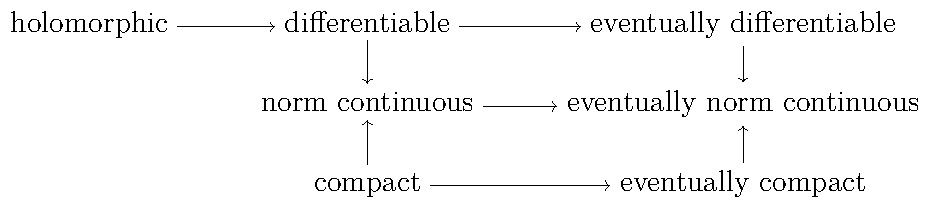
\includegraphics[width=0.8\textwidth]{./tikz-images/tikz-chap-a2.pdf}
\end{center}
% \begin{tikzcd}
% \text{holomorphic} \arrow[r] 
% & \text{differentiable} \arrow[r] \arrow[d] & \text{eventually differentiable} \arrow[d] \\
% & \text{norm continuous} \arrow[r] & \text{eventually norm continuous}  \\
% & \text{compact} \arrow[u] \arrow[r] & \text{eventually compact} \arrow[u]
% \end{tikzcd}
%% --
\index{semigroup!eventually compact semigroup|)}
\index{semigroup!differentiable semigroup}
\index{semigroup!holomorphic semigroup}
\index{semigroup!norm continuous semigroup}

All these classes are different.
This is shown by the following examples.
%%
%%
\begin{example}\label{ex:a2-1.27}
The nilpotent shift semigroup (Section~\ref{subsec:a1-2.6}) is obviously eventually differentiable, eventually compact and eventually norm continuous.
But it is not norm continuous and consequently not differentiable or compact.
\end{example}
%% --
\begin{example}\label{ex:a2-1.28}
We consider multiplication semigroups (see Section~\ref{subsec:a1-2.3}).
Let $E = C_{0}(X)$, where $X$ is a locally compact space, or $E = L^{p}(X,\Sigma,\mu)$, where $1 \leq p < \infty$ and $(X,\Sigma,\mu)$ is a $\sigma$-finite measure space.
Let $m \colon X \to \C$ be continuous (\resp measurable) such that $[\text{ess}]\text{-}\sup_{x \in X} \Re(m(x)) < \infty$.

Then $Af = m \cdot f$ with domain $D(A) = \{f \in E \colon m \cdot f \in E\}$ is the generator of the semigroup $(T(t))_{t \geq 0}$ given by
%%--
\[
    (T(t)f)(x) = \eu^{tm(x)}f(x), \quad (t \geq 0, x \in X, f \in E )\, .
\]
%%--
Observe that $\sigma(A) = \closure{m(X)}$ in case $E = C_{0}(X)$ and 
%%
\[
\sigma(A) = [\text{ess}]\text{-}\Image{m} \coloneq \{\lambda \in \C \colon \mu(\{x \in X \colon |m(x)-\lambda| < \epsilon\}) \neq 0 \text{ for all } \epsilon > 0\} 
\]
%% 
if\/ $E = L^{p}$ (see Section~\ref{subsec:a1-2.3}).
Consequently, 
%
\[
	s(A) = \omega_{0}(A) = [\text{ess}]\text{-}\sup_{x \in X} \Re(m(x)).
\]
%
\begin{enumerate}[\upshape (i), wide, labelindent=.25em]
\item \label{ex:a2-1.28-1}
\textit{The semigroup is norm continuous for $t > 0$ if and only if it is eventually norm continuous if and only if 
$\{\lambda \in \sigma(A) \colon \Re(\lambda) \geq b\}$ 
is bounded for every $b \in \R$.
Thus the property proved in Theorem~\ref{thm:a2-1.20}   characterizes generators of eventually norm continuous semigroups in the case that the semigroup consists of multiplication operators.}
\index{semigroup!eventually norm continuous semigroup|)}
%% --
\begin{proof}
Assume that $\{\lambda \in \sigma(A) \colon \Re(\lambda) \geq b\}$ is bounded for every $b \in \R$.
Let $t' > 0$.
We show that the semigroup is norm continuous at $t'$.
Take $\epsilon > 0$ and $b \in \R$ such that $2\eu^{t'b/2} < \epsilon$.

If\/ $\Re(m(x)) \leq b$, then
%%--
\[
    \left|\eu^{tm(x)} - \eu^{t'm(x)}\right| \leq \eu^{t\Re(m(x))} + \eu^{t'\Re(m(x))} \leq 2\eu^{t'b/2} < \epsilon
\]
%%--
whenever $|t-t'| \leq t'/2$.

By hypothesis, the set 
%
\[
	H \coloneq \{m(x) \colon x \in X, \Re(m(x)) \geq b\} 
\]
%
in the case $E = C_{0}(X)$ 
and%
\[
	 H \coloneq \{\lambda \in \C \colon \Re(\lambda) \geq b \text{ and for all } \eta > 0,  
\mu(\{x \in X \colon |m(x)-\lambda| < \eta \}) \neq 0\}
\]
%
in the case $E = L^{p}$ is a bounded subset of\/ $\C$.
Thus $\lim_{t \to t'} |\eu^{tz} - \eu^{t'z}| = 0$ uniformly for $z \in H$.
Hence there exists $\delta \in (0,t'/2]$ such that
%% --
\[
[\text{ess}]\text{-}\sup\left\{\left|\eu^{tm(x)} - \eu^{t'm(x)}\right| \colon x \in X, \Re(m(x)) > b\right\} < \epsilon
\] 
%% --
whenever $|t-t'| < \delta$.
Together with the inequality above, we obtain that 
%%
\[
\|T(t) - T(t')\| = [\text{ess}]\text{-}\sup\left\{\left|\eu^{tm(x)} - \eu^{t'm(x)}\right| \colon x \in X\right\} < \epsilon
\]
%% 
whenever $|t-t'| < \delta$.
We have shown that the semigroup is norm continuous for $t > 0$ whenever $\{\lambda \in \sigma(A) \colon \Re(\lambda) \geq b\}$ is bounded for all $b \in \R$.
\end{proof}
%% --
\item \label{ex:a2-1.28-2}
\textit{The semigroup is right-sided differentiable at a point $t > 0$ 
if and only if there exists $c > 0$ such that}
%
\[
	\{\lambda \in \C \colon |\Im(\lambda)| > c \cdot \eu^{-t\Re(\lambda)}\} \subseteq \rho(A) .
\]
%
\begin{proof}
The semigroup is right-sided differentiable at a point $t > 0$ if and only if the following equivalent assertions hold.
\begin{enumerate*}[\upshape(a)]
\item
$T(t)E \subseteq D(A)$,
\item
$\eu^{tm} \cdot f \cdot m \in E$ for all $f \in E$,
\item
$\eu^{tm} \cdot m$ is [essentially] bounded,
\item
$\eu^{t\Re(m)} \cdot \Im(m)$ is [essentially] bounded, 
\item
there exists $c > 0$ such that 
$[\text{ess}]\text{-}\Image{m} \subseteq 
\left\{\lambda \in \C \colon \eu^{t\Re(\lambda)}\lvert\Im(\lambda)\rvert \leq c\right\}$, 
\item
there exists $c > 0$ such that 
$\left\{\lambda \in \C \colon \lvert\Im(\lambda)\rvert > c \cdot \eu^{-t\Re(\lambda)}\right\} \subseteq \rho(A)$.
\qedhere
\end{enumerate*}
\end{proof}
%% --
\item \label{ex:a2-1.28-3}
\textit{$(T(t))_{t \geq 0}$ is a bounded holomorphic semigroup of angle $\theta$ if and only if} 
%
\[
	S(\theta + \pi/2) \subseteq \rho(A) .
\]
%
\begin{proof}
The condition is necessary by Theorem~\ref{thm:a2-1.12}.
Conversely, if\/ $S(\theta + \pi/2) \subseteq \rho(A)$, then one verifies directly that 
%%--
\[
(T(z)f)(x) = \eu^{z \cdot m(x)}f(x) \quad (f \in E, x \in X) 
\]
%%-- 
defines a family $(T(z))_{z \in S(\theta)}$ of bounded operators satisfying conditions (i) and (ii)
of Definition~\ref{def:a2-1.11}.
\end{proof}
%% --
\item \label{ex:a2-1.28-4}
\textit{Choosing $X = \N$ and the counting measure we have $E = c_{0}$ or $\ell^{p}$.
Then $A$ has a compact resolvent if }
%
\[
	\lim_{n \to \infty} \abs{m(n)} = \infty .
\]
%
In fact, let $\lambda > s(A)$.
Then $(R(\lambda,A)f)(n) = (\lambda-m(n))^{-1}f(n)$.
Hence $R(\lambda,A)$ is compact if and only if\/ $((\lambda-m(n))^{-1})_{n \in \N} \in c_{0}$. 

The semigroup is compact if and only if it is eventually compact if and only if 
%% --
\[
\lim_{n \to \infty} \Re(m(n)) = -\infty.
\]
%% --
\end{enumerate}
%% --
Now it is easy to give concrete examples. 
Again let $X = \N$, so that $E = c_{0}$ or $\ell^{p}$.
%% --
\begin{enumerate}[\upshape(i)]%\label{ex:a2-1.28-5}

\item
Let $m(n) = -n + \iu\,\eu^{n^{2}}$.
Then the semigroup is compact and (consequently) norm continuous for $t > 0$, but it is not eventually differentiable.

\item
Let $m(n) = -n + \iu\,\eu^{s'n}$.
Then the semigroup is differentiable for $t > s'$ but not differentiable at $t \in [0,s')$.

\item
If\/ $m(n) = -n + \iu\, n^{2}$, then the semigroup is differentiable but not holomorphic.

\end{enumerate}
%% --
\end{example}	

\subsection{Perturbation of Generators} \label{subsec:a2-1.se8}
\index{semigroup!bounded perturbation}
A useful way to construct new semigroups out of a given one is by additive perturbation.%
%% --
\begin{theorem}\label{thm:a2-1.29}
Let $A$ be the generator of a strongly continuous semigroup $(T(t))_{t \geq 0}$ and let $B \in \LE$.
Then $A + B$ with domain $D(A+B) = D(A)$ is the generator of a strongly continuous semigroup $(S(t))_{t \geq 0}$.
\end{theorem}
%% --
It is possible to express the new semigroup $(S(t))_{t \geq 0}$ by known objects.
The product formula
%%--
\begin{equation}\label{eq:a2-1.8}
    S(t)f = \lim_{n \to \infty} \left( T(t/n)\eu^{t/n \cdot B} \right)^{n} f
\end{equation}
%%--
holds for all $t \geq 0$ and $f \in E$.

Moreover, $S(t)$ is the solution of the following integral equation
%%--
\begin{equation}\label{eq:a2-1.9}
    S(t)f = T(t)f + \int_{0}^{t} T(t-s)BS(s)f\ds \quad (t \geq 0, f \in E).
\end{equation}
%%--

Let $S_{0}(t) = T(t)$ and
%%--
\begin{equation}\label{eq:a2-1.10}
    S_{n}(t)f = \int_{0}^{t} T(t-s)BS_{n-1}(s)f\ds \quad (f \in E)
\end{equation}
%%--
for $n \in \N$. Then
%%--
\begin{equation}\label{eq:a2-1.11}
    S(t) = \sum_{n=0}^{\infty} S_{n}(t),
\end{equation}
%%--
where the series converges in the operator norm uniformly on bounded intervals.
We refer to \textcite[III.1]{davies:1980}, \textcite[I.6]{goldstein:1985a} or \textcite[Chapter 3]{pazy:1983} for these results.

Several special properties discussed above are preserved by bounded perturbations.
%% --
\begin{theorem} \label{thm:a2-1.30}
Let $(T(t))_{t \geq 0}$ be a strongly continuous semigroup with generator $A$, and let $B \in \LE$.
%% --
\begin{enumerate}[\upshape(i)]
\item
If\/ $(T(t))_{t \geq 0}$ is holomorphic or norm continuous or compact, then so is the semigroup 
$(S(t))_{t \geq 0}$ 
generated by $A+B$.

\item
If\/ $A$ has a compact resolvent then so has $A+B$.

\item
Let $t_{0} \geq 0$.
If\/ $(T(t))_{t \geq 0}$ is norm continuous for $t > t_{0}$ and if 
$B$ is compact, then $(S(t))_{t \geq 0}$ is also norm continuous for $t > t_{0}$.

\end{enumerate}
%% --
\end{theorem}
%% --
\begin{proof}
If\/ $(T(t))_{t \geq 0}$ is norm continuous for $t > 0$, then $S_{n}(t)$ in Eq.~\myeqpageref{eq:a2-1.10} is norm continuous at $t > 0$ for every $n$.
Thus $(S(t))_{t \geq 0}$ is norm continuous at $t > 0$ by Eq.~\myeqpageref{eq:a2-1.11}.
There exists $\lambda_{0} \in \R$ such that 
%
\[
	\|R(\lambda,A)\| \leq (2\|B\|)^{-1} \text{ for } \Re(\lambda) \geq \lambda_{0} .
\]
%
Hence $(\Id - B \cdot R(\lambda,A))^{-1}$ exists for $\Re(\lambda) \geq \lambda_{0}$.
Since 
%%
\[
(\lambda -(A+B))f = (\Id - BR(\lambda,A))(\lambda - A)f  \quad \text{ for all } \quad f \in D(A),
\]
%%
it follows that $(\lambda-(A+B))^{-1}$ exists and is given by
%%--
\begin{equation}\label{eq:a2-1.12}
    R(\lambda,A+B) = R(\lambda,A)(\Id-BR(\lambda,A))^{-1}
\end{equation}
%%--
whenever $\Re(\lambda) \geq \lambda_{0}$.
Now if\/ $A$ generates a holomorphic semigroup, there exists $M \geq 0$ such that $\|R(\lambda_{0}+\im\eta,A)\| \leq M/|\eta|$ for all $\eta \in \R$.
Consequently, 
%%--
\[
\|R(\lambda_{0}+\im\eta,A+B)\| \leq \|(\Id-BR(\lambda_{0} + \iu \eta,A))^{-1}\| \cdot M/|\eta| \leq 2M/|\eta|
\]
%%--
for all $\eta \in \R$.
Thus $A + B$ generates a holomorphic semigroup by the corollary of Theorem~\ref{thm:a2-1.14}.
Moreover, it follows from Eq.~\myeqpageref{eq:a2-1.12}  that $R(\lambda,A+B)$ is compact whenever $R(\lambda,A)$  is compact.
Consequently, by Theorem~\ref{thm:a2-1.25} and the  assertion proved above, $(S(t))_{t \geq 0}$ is compact whenever $(T(t))_{t \geq 0}$ is compact.

Finally assume that $B$ is compact and $t_{0} \geq 0$ such that $(T(t))_{t \geq 0}$ 
is norm continuous for $t > t_{0}$.
Fix $t > t_{0}$.
Denote by $U$ the unit ball of\/ $E$ and fix $s \in (0,t]$.
Then
%%--
\[
    \lim_{h \to 0} (T(t+h-s) - T(t-s))f = 0
\]
%%--
for all $f \in \overline{BS(s)U} \eqqcolon K$.

Since $K$ is compact it follows that the limit exists uniformly with respect to $f \in K$, \ie  
$\lim_{h \to 0} \|(T(t+h-s) - T(t-s))BS(s)\| = 0$.
It follows from the dominated convergence theorem that
%%--
\begin{equation}\label{eq:a2-1.13}
    \lim_{h \to 0} \int_{0}^{t} \|(T(t+h-s) - T(t-s))BS(s)\|\ds = 0.
\end{equation}
%%--
Using  Eq.~\myeqpageref{eq:a2-1.9}  we obtain 
\begin{align*}
	\|S(t+h) - S(t)\| &\leq \|T(t+h) - T(t)\| \\
	&\quad +  \left\| \int_{0}^{t+h} T(t+h-s)BS(s)\ds 
	-  \int_{0}^{t} T(t-s)BS(s)\ds \right\| \\
	&\leq \|T(t+h) - T(t)\| + \int_{t}^{t+h} \|T(t+h-s)BS(s)\| \ds \\ 
	&\quad + \int_{0}^{t} \|(T(t+h-s) - T(t-s))BS(s)\|\ds \to 0 
\end{align*}
%% --
when  $h \to 0$. 	
\end{proof}
%% --
In Part-III, Example~\ref{ex:c4-2.15} a generator $A$ of an eventually differentiable and eventually compact semigroup and a bounded operator $B$ will be given such that the semigroup generated by $A+B$ is not eventually norm continuous.

Using Theorem~\ref{thm:a2-1.29}   we now prove a perturbation result due to \textcite{deschschappacher:1984}.
Instead of assuming that $B \in \mathcal{L}(E)$ we assume that $B \in \mathcal{L}(D(A))$.
The short proof given below is due to G.\,Greiner.
%% --
\begin{theorem}\label{thm:a2-1.31}
Let $(T(t))_{t \geq 0}$ be a strongly continuous semigroup with generator $A$.
Assume that $B \colon D(A) \to D(A)$ is linear and continuous for the graph norm on $D(A)$.
%% --
Then $A + B$ with domain $D(A + B) = D(A)$ is the generator of a strongly continuous semigroup.
Moreover, there exists a bounded operator $C$ on $E$ such that $A + B$ is similar to $A + C$.
\end{theorem}
\index{operator!similar}
\begin{proof}
We first show that $(\Id - BR(\lambda,A))$ is invertible for some $\lambda \in \C$.
Choose $\lambda_{0} \in \rho(A)$.
Then $S \coloneq (\lambda_{0}-A)BR(\lambda_{0},A) \in \mathcal{L}(E)$.
Let $\lambda > s(A)$ be so large that $\|SR(\lambda,A)\| < 1$.
Then 
%%
\[
\Id - (\lambda_{0} - A)BR(\lambda_{0},A)R(\lambda,A) = (\Id - SR(\lambda,A))
\]
%%
is invertible.
Consequently, also $(\Id -BR(\lambda,A))^{-1}$ exists
(since 
%%
\[
\sigma(TR(\lambda_{0},A)) \setminus \{0\} 
= \sigma(R(\lambda_{0},A)T) \setminus \{0\}\,
\]
%%
where  $T = (\lambda_{0}-A)BR(\lambda,A)\, $).

Let $C = (A-\lambda)B(A-\lambda)^{-1} \in \mathcal{L}(E)$.
Then $A + C$ is the generator of a strongly continuous semigroup by Theorem~\ref{thm:a2-1.29}. 
We show that $A + B$ is similar to $A + C$.
In fact, let $U = (\Id - BR(\lambda,A))$.
Then $U$ is an isomorphism on $E$ such that $U(D(A)) = D(A)$. Moreover,
\begin{align*}		
U(A+C)U^{-1} &= U(A - \lambda+C)U^{-1} + \lambda \\
&= U[(A - \lambda) - (A-\lambda)BR(\lambda,A)]U^{-1} + \lambda \\
&= U(A - \lambda)[\Id - BR(\lambda,A)]U^{-1} + \lambda \\
&= U(A - \lambda) + \lambda \\
&= A - \lambda + B + \lambda \\
&= A + B.	\tag*{\qedsymbol}%&&\qedhere
\end{align*}
\let\qedsymbol\relax
\end{proof}
%% --
\begin{corollary}\label{cor:a2-1.32}
Keeping the hypotheses and notations of Theorem~\ref{thm:a2-1.31} denote by 
$(S(t))_{t\geq 0}$ the semigroup generated by $A+B$.
%% --
\begin{enumerate}[\upshape(i)]
\item
If\/ $(T(t))_{t\geq 0}$ is norm continuous or compact or holomorphic, then $(S(t))_{t\geq 0}$ has the corresponding properties.

\item
If\/ $B$ is compact as an operator on $D(A)$ endowed with the graph norm and if\/ $(T(t))_{t\geq 0}$ is eventually norm continuous, then so is $(S(t))_{t\geq 0}$.
\end{enumerate}
%% --
\end{corollary}
%% --
\begin{proof}
Both assertions follow from Theorem~\ref{thm:a2-1.30}  because $(U^{-1}S(t)U)_{t\geq 0}$ has $A+C$ as generator.
\end{proof}
%% --
%% -- Stand 2026-03-10
%% –
\subsection{Domains of Uniqueness} \label{subsec:a2-1.se9}%
\index{semigroup!domains of uniqueness}
%% --
Given a semigroup $(T(t))_{t \geq 0}$,  
it is frequently difficult to determine the precise domain of its generator $A$.
So it is important to know which (possibly strict) subspaces of\/ $D(A)$ determine the semigroup uniquely.
This can be formulated more precisely in the following way.
%% --
\begin{quote}
\textit{Let $D_{0}$ be a subspace of\/ $D(A)$ and consider the restriction $A_{0}$ of\/ $A$ to $D_{0}$.
Under which condition on $D_{0}$ is $A$ the only extension of\/ $A_{0}$ which is a generator?}
\end{quote}
%% --
One obvious condition is that $D_{0}$ is a core.
\index{core}
In fact, in that case, $A$ is the closure of\/ $A_{0}$.
Since every generator $B$ extending $A_{0}$ is closed, it follows that $A \subseteq B$ and hence $A = B$ since 
$\rho(A) \cap \rho(B) \neq \emptyset$.

We now show that cores are the only domains of uniqueness.
%% --
\begin{theorem}\label{thm:a2-1.33}
Let $A$ be the generator of a semigroup and $D_{0}$ a subspace of\/ $D(A)$.
Consider the restriction $A_{0}$ of\/ $A$ to $D_{0}$.
If\/ $D_{0}$ is not a core of\/ $A$, then there exists an infinite number of extensions of\/ $A_{0}$ which are generators.
\end{theorem}
%% --
\begin{proof}
If\/ $D_{0}$ is not dense in $D(A)$ with respect to the graph norm, then there exists a non-zero linear form $\phi$ on $D(A)$ which is continuous for the graph norm such that $\phi(f) = 0$ for all $f \in D_{0}$. 
Let $u \in D(A)$ and $B \colon D(A) \to D(A)$ be given by $Bf = \phi(f)u$ for all $f \in D(A)$.
Then $B$ is continuous for the graph norm.
So by Theorem~\ref{thm:a2-1.31}   the operator $A+B$ with domain $D(A)$ is a generator.
Clearly, $A+B \neq A$ if\/ $u \neq 0$ but $Af+Bf = Af$ for all $f \in D_{0}$.
It is obvious that an infinite number of generators can be constructed in that way.
\end{proof}
%% --
\begin{corollary}\label{cor:a2-1.34}
Let $(T(t))_{t\geq 0}$ be a strongly continuous semigroup with generator $A$.
Let $D_{0}$ be a dense subspace of\/ $E$.
Assume that $D_{0} \subseteq D(A)$ and $T(t)D_{0} \subseteq D_{0}$ for all $t \geq 0$.
Then $D_{0}$ is a core.
\end{corollary}
%% --
\begin{proof}
Let $(S(t))_{t\geq 0}$ be a semigroup with generator $B$ such that $B_{\vert D_{0}} = A_{\vert D_{0}}$, and take $f \in D_{0}$.
Then $u(t) \coloneq T(t)f$ satisfies 
%%
\[
u(0) = f\,  \text{ and } \,\dot{u}(t) = AT(t)f = BT(t)f = Bu(t) \quad (t \geq 0).
\]
%%
Since $v(t) = S(t)f$ $(t \geq 0)$ also is a solution of the Cauchy problem defined by $B$ with initial value $f$ it follows that $S(t)f = T(t)f$ $(t\geq 0)$.
Since $D_{0}$ is dense in $E$, it follows that $S(t) = T(t)$ $(t \geq 0)$.
\end{proof}
\index{resolvent|)}
%% –
%% --
\section{Contraction Semigroups and Dissipative Operators}\label{sec:a2-2}%
\index{semigroup!contraction semigroup|(}
\index{dissipative operator}
%% --
\hspace{1cm}{\Large by Wolfgang Arendt}
\vspace{.5cm}
\newline
%% --
The Hille-Yosida theorem gives a characterization of generators in terms of the resolvent of the operator.
However, given an operator $A$, frequently it is difficult to compute the resolvent and its powers.
So it is desirable to find conditions more immanent on $A$.
This is possible for generators of contraction semigroups.

For later purposes (see Part-II, Chapter~\ref{chap:b2} and Part-III, Chapter~\ref{chap:c2}) it will be useful not only to consider semigroups which are contractive with respect to the norm but to consider more general sublinear functionals than the norm as well.

So our setting is the following.
By $E$ we denote a real Banach space throughout and $p \colon E \to \R$ is a continuous sublinear function; \ie $p$ satisfies
%%
\begin{equation}\label{eq:a2-2.1}
\begin{split}
p(f+g) &\leq p(f) + p(g) \quad (f, g \in E), \\%\label{eq:a2-2.1} \\
p(\lambda f) &= \lambda p(f) \quad (f \in E, \lambda \geq 0). %\label{eq:a2-2.2}
\end{split}
\end{equation}
%% --
The continuity of\/ $p$ implies that there exists a constant $c > 0$ such that
%% --
\begin{equation}\label{eq:a2-2.3}
	|p(f)| \leq c\|f\| \quad (f \in E).
\end{equation}
%% -- 
Moreover, it follows from Eq.~\myeqpageref{eq:a2-2.1} that
%% --
\begin{equation*}\label{eq:a2-2.4}
	p(f) + p(-f) \geq p(0) = 0 \quad (f \in E).
\end{equation*}
%% --
A bounded operator $T$ on $E$ is called \emph{p-contractive} if\/ $p(Tf) \leq p(f)$ for all $f \in E$.
Similarly, a semigroup $(T(t))_{t\geq 0}$ is called \emph{p-contractive} if\/ $T(t)$ is $p$-contractive for all $t \geq 0$.
Of course, the most important case in this section is when $p$ is the norm function $N$ given by $N(f) = \|f\|$ $(f \in E)$.
An $N$-contractive operator is just a contraction in the usual sense.
%% –
\begin{remark*} \label{rem:a2-2.1-kgk}
However in Part-II, Chapter~\ref{chap:b2} and Part-III, Chapter~\ref{chap:c2} it will be important to dispose of a variety of sublinear functionals other than $N$.
For example, we will consider $N^{+}$ on $C([0,1])$ given by 
%
\[
	N^{+}(f) = \sup_{x \in [0,1]} f^{+}(x) = \|f^{+}\|_{\infty} .
\]
%
Then a bounded operator $T$ is $N^{+}$-contractive if and only if\/ $T$ is positive and $\|T\| \leq 1$.
\end{remark*}
%% --
We first want to solve the following problem.
%% --
\begin{quote}
\textit{Given the generator $A$ of a semigroup $(T(t))_{t\geq 0}$ find a condition on $A$ which is equivalent to $T(t)$ being $p$-contractive for all $t \geq 0$.}
\end{quote}
%% --
The \emph{subdifferential} $\ddp$ of\/ $p$ at $f$ is defined by
\begin{equation}\label{eq:a2-2.5}
\ddp(f) = \{\phi \in E' \colon \dualp{g,\phi} \leq p(g) \text{ for all } g \in E, \dualp{f,\phi} = p(f) \}.
\end{equation}
It follows from the Hahn-Banach theorem that $\ddp(f) \neq \emptyset$ for all $f \in E$.
%% --
\begin{definition}\label{def:a2-2.1}
\index{half-norm!p-dissipative}
An operator $A$ on $E$ is called \emph{p-dissipative} if for all $f \in D(A)$ there exists $\phi \in \ddp(f)$ such that $\dualp{Af,\phi} \leq 0$ 
and $A$ is called \emph{strictly $p$-dissipative} if for all $f \in D(A)$ the inequality $\dualp{Af,\phi} \leq 0$ holds for all $\phi \in \ddp(f)$.
\end{definition}
%%
For convenience we want to have a distinctive name for the norm function.
So we denote by $N \colon E \to \R$ the function given by $N(f) = \|f\|$ throughout.
Then Eq.~\myeqpageref{eq:a2-2.5} can be written in the form
%% --
\begin{equation}\label{eq:a2-2.6}
\dN(f) = \{\phi \in E' \colon \|\phi\|\leq 1, \dualp{f,\phi} = \|f\|\}.
\end{equation}
%% --
A (strictly) $N$-dissipative operator is simply called (strictly) \emph{dissipative}, which is in accordance with the usual nomenclature.

\phantom{x}
%% –
\begin{examples}\label{ex:a2-2.2}  ~ 
%% --
\begin{enumerate}[\upshape(i), wide, labelindent=.25em]

\item \label{ex:a2-2.2.1}
Let $E = C([0,1])$ and $f \in E$.
Then there exists $x \in [0,1]$ such that $|f(x)| = \|f\|_{\infty}$.
Define $\phi \in E'$ by 
%
\[
	\dualp{g,\phi} = \sign(f(x))\,g(x) .
\]
%
Then $\phi \in \dN(f)$.
Note that $\dN(f)$ may be an infinite set.
%%--
\item \label{ex:a2-2.2.2}
Let $H$ be a Hilbert space and $ 0 \neq f \in H$. %, $f \neq 0$.
Then  $\dN(f) = \{\phi_{f}\}$ where 
%
\[
%	\dualp{g,\phi_{f}} = ( \|f\|\,(g \vert f) )^{-1} .
    \dualp{g,\phi_{f}} = \|f\|^{-1}(g \vert f) .
\]
%
%%--
\item \label{ex:a2-2.2.3}
$A - \|A\|\Id$ is strictly dissipative for every bounded operator $A$.
\end{enumerate}
\end{examples}
%% –
\begin{proposition}\label{prop:a2-2.3}
Let $A$ be an operator on $E$.
Then $A$ is $p$-dissipative if and only if
%% --
\begin{equation} \label{eq:a2-2.7}
p(f) \leq p(f - tAf) \text{ for all } f \in D(A) \text{ and } t > 0.
\end{equation}
%% --
If in particular $(w,\infty) \subseteq \rho(A)$ for some $w \geq 0$, then $A$ is $p$-dissipative if and only if
%% --
\begin{equation}\label{eq:a2-2.8}
p(\lambda R(\lambda,A)f) \leq p(f) \text{ for all } f \in E, \lambda > w.
\end{equation}
\end{proposition}
%% --
\begin{proof}
Assume that $A$ is $p$-dissipative.
Let $f \in D(A)$ and $t > 0$.
There exists  $\phi \in \ddp(f)$ such that $\dualp{Af,\phi} \leq 0$.
Hence, 
%%
\[
p(f) = \dualp{f,\phi} = \dualp{f - tAf + tAf, \phi} \leq \dualp{f - tAf,\phi} \leq p(f - tAf).
\] 
%%
So Eq.~\myeqpageref{eq:a2-2.7} holds.

Conversely, let $f \in D(A)$.
For every $t > 0$ choose $\phi_{t} \in \ddp(f - tAf)$.
Then 
%
\[
	\pm \dualp{g,\phi_{t}} \leq p(\pm g) \leq c\|g\|
\]
%
for all $g \in E$, $t > 0$.
Thus the net $(\phi_{t})_{t>0}$ is bounded.
Consequently it possesses a $\sigma(E',E)$-limit point $\phi$ as $t \to 0$.
We show that $\phi \in \ddp(f)$ and $\dualp{Af,\phi} \leq 0$.

Since $\dualp{g,\phi_{t}} \leq p(g)$ for all $t > 0$, 
it follows that $\dualp{g,\phi} \leq p(g)$ $(g \in E)$.
Moreover, 
%
\[
	\dualp{f,\phi_{t}} - t\dualp{Af, \phi_{t}} = p(f - tAf) \quad (t > 0) .
\]
%
Letting $t \to 0$ yields $\dualp{f,\phi} = p(f)$.

We have proved that $\phi \in \ddp(f)$.
By hypothesis we have for all $t > 0$,
%
\begin{equation*}
\begin{split}
	p(f) &\leq p(f-tAf) = \dualp{f-tAf,\phi_{t}} \\
&= \dualp{f,\phi_{t}} - t\dualp{Af,\phi_{t}} \leq p(f) - t \dualp{Af,\phi_{t}} .
\end{split}
\end{equation*}
%
Consequently $\dualp{Af,\phi_{t}} \leq 0$ for all $t > 0$.
Thus $\dualp{Af,\phi} \leq 0$.
\end{proof}
%%
%% --
\begin{remark}\label{rem:a2-2.4}
The function $p$ is convex.
So the one-sided Gateaux-derivatives
%% –
\begin{align*}
D^{+}_{g} p(f) &= \lim_{t \downarrow 0} \frac{1}{t} (p(f+tg) - p(f)) 
\intertext{and}
D^{-}_{g} p(f) &= \lim_{t \uparrow 0} \frac{1}{t} (p(f+tg) - p(f))
\end{align*}
%% –
exist and satisfy $D^{-}_{g}p(f) \leq D^{+}_{g}p(f)$ for all $f, g \in E$ (\cf \textcite{moreau:1966}).
Moreover,
%% --
\begin{equation}\label{eq:a2-2.9}
D^{+}_{g} p(f) = \sup \{\dualp{g,\phi} \colon \phi \in \ddp(f)\},
\end{equation}
%% --
\begin{equation}\label{eq:a2-2.10}
D^{-}_{g} p(f) = \inf \{\dualp{g,\phi} \colon \phi \in \ddp(f)\}.
\end{equation}
%% --
Thus $A$ is $p$-dissipative if and only if\/ $D^{-}_{Af} p(f) \leq 0$, and $A$ is strictly $p$-dissipative if and only if\/ $D^{+}_{Af} p(f) \leq 0$ for all $f \in D(A)$.
\end{remark}
%% --
\begin{corollary}\label{cor:a2-2.5}
Let $A$ be a closable operator.
If\/ $A$ is $p$-dissipative, then so is its closure.
\end{corollary}
%% --
\begin{theorem}\label{thm:a2-2.6}
Let $p$ be a continuous sublinear functional on a real Banach space $E$.
Let $A$ be the generator of a strongly continuous semigroup $(T(t))_{t\geq 0}$.
The following assertions are equivalent.
%% --
\begin{enumerate}[\upshape (a)]
\item \label{thm:a2-2.6.1}
$p(T(t)f) \leq p(f)$ for all $t \geq 0$, $f \in E$.

\item \label{thm:a2-2.6.2}
$A$ is strictly $p$-dissipative.
 
\item \label{thm:a2-2.6.3}
There exists a core $D$ of\/ $A$ such that $A_{\vert D}$ is $p$-dissipative.
\end{enumerate}
\end{theorem}
%% --
\begin{proof}
Assume that~\ref{thm:a2-2.6.1} holds.
Let $f \in D(A)$, $\phi \in \ddp(f)$.
Then 
\begin{align*}
	\dualp{Af,\phi} &= \lim_{t\to 0} \frac{1}{t} (\dualp{T(t)f,\phi} - \dualp{f,\phi}) \\
	&= \lim_{t\to 0} \frac{1}{t} (\dualp{T(t)f,\phi} - p(f)) \\
	&\leq \limsup_{t\to 0} \frac{1}{t} (p(T(t)f) - p(f)) \leq 0. 
\end{align*}
This proves~\ref{thm:a2-2.6.2}. 

It is trivial that~\ref{thm:a2-2.6.2} implies~\ref{thm:a2-2.6.3}.  
So let us assume~\ref{thm:a2-2.6.3}. 
Then it follows from Corollary~\ref{cor:a2-2.5}   that $A$ is $p$-dissipative.
Hence, by Eq.~\myeqpageref{eq:a2-2.8},  
%
\[
	p(\lambda R(\lambda,A)g) \leq p(g) \quad\text{for all $g \in E$, $\lambda > \max\{\omega_{0}(A),0\}$}.
\]
%
Hence $\lambda R(\lambda,A)$ is $p$-contractive for $\lambda > \max\{\omega_{0}(A),0\}$.
This implies that $T(t)$ is $p$-contractive by the formula \myeqpageref{eq:a2-1.3}, 
%% –
\begin{equation*}
T(t) = \lim_{n\to\infty} \left( \frac{n}{t} R\left( \frac{n}{t},A \right) \right)^{n} 
	\text{ (strongly) for } t \geq 0. 
	\qedhere
\end{equation*}
%% --
\end{proof}
%% --
We have shown that for generators, $p$-dissipativity is equivalent to $p$-contractivity of the semigroup.
Now we will consider a $p$-dissipative operator $A$ (which is not a generator a priori) and investigate under which additional hypotheses $A$ is the generator of a (necessarily $p$-contractive) semigroup.
At first we present some consequences of $p$-dissipativity.
%% –
\begin{theorem}\label{thm:a2-2.7}
Let $A$ be a $p$-dissipative operator.
If\/ $D(A)$ is dense, then $A$ is strictly $p$-dissipative.
\end{theorem}
%% –
\begin{proof}
Let $f \in D(A)$, $\phi \in \ddp(f)$.
Then for every $t > 0$ and $g \in D(A)$ we have
% \begin{align*}
% \dualp{Af,\phi} 
% &= \frac{1}{t}(\dualp{f + tAf,\phi} - \dualp{f,\phi}) \leq \frac{1}{t}(p(f + tAf) - p(f)) \\
% &\leq \frac{1}{t}(p(f + tg) + tp(Af - g) - p(f)) \\
% &\leq \frac{1}{t}(p((\Id - tA)(f + tg)) + tp(Af - g) - p(f)) \quad \text{(by Eq.~\myeqpageref{eq:a2-2.7}\,)} \\ %% (2.7))
% &\leq \frac{1}{t}(p(f) + tp(g - Af) + t^2p(-Ag) + tp(Af - g) - p(f)) \\
% &\leq \frac{1}{t}(2tc\|g - Af\| + t^2c\|Ag\|) \quad \text{(by (2.3))} \\
% &= 2c\|g - Af\| + tc\|Ag\|.
% \end{align*}
%% --
\begin{align*}
\dualp{Af,\phi} 
&= \frac{1}{t}(\dualp{f + tAf,\phi} - \dualp{f,\phi}) \leq \frac{1}{t}(p(f + tAf) - p(f)) \\
&\leq \frac{1}{t}(p(f + tg) + tp(Af - g) - p(f)) \\
&\leq \frac{1}{t}(p((\Id - tA)(f + tg)) + tp(Af - g) - p(f)) \\
&\qquad \text{(by Eq.~\myeqpageref{eq:a2-2.7})} \\
&\leq \frac{1}{t}(p(f) + tp(g - Af) + t^2p(-Ag) + tp(Af - g) - p(f)) \\
&\leq \frac{1}{t}(2tc\|g - Af\| + t^2c\|Ag\|) \quad \text{(by Eq.~\eqref{eq:a2-2.3})} \\
&= 2c\|g - Af\| + tc\|Ag\|.
\end{align*}
%% --
Letting $t \to 0$ we obtain $\dualp{Af,\phi} \leq 2c\|g - Af\|$ for all $g \in D(A)$.
Since $D(A)$ is dense in $E$, this implies that $\dualp{Af,\phi} \leq 0$.
\end{proof}
%% --
We now impose stronger conditions on $p$.
\index{half-norm|(}
A continuous sublinear function $p \colon E \to \R$ is called a \emph{half-norm} if
%%--
\begin{equation}\label{eq:a2-2.11}
p(f) + p(-f) > 0 \text{ whenever } f \neq 0;
\end{equation}
%%--
and $p$ is called a \emph{strict half-norm} if in addition there exists some constant $d > 0$ such that
%%--
\begin{equation}\label{eq:a2-2.12}
p(f) + p(-f) \geq d\|f\| \text{ for all } f \in E.
\end{equation}
%%--
If\/ $p$ is a half-norm, then
\begin{equation}\label{eq:a2-2.13}
\|f\|_p = p(f) + p(-f) \quad (f \in E)
\end{equation}
%%--
defines a norm on $E$ which is equivalent to the given norm if and only if\/ $p$ is strict.

%% –
\begin{remark}\label{rem:a2-2.8}
Every half-norm $p$ induces a closed proper cone 
%%
\[
E_{p} \coloneq \{f \in E \colon p(-f) \leq 0\}
\] 
%%
on $E$.
Any $p$-contractive operator $T$ on $E$ leaves the cone $E_{p}$ invariant (\ie  $T$ is positive for the corresponding ordering).

Conversely, given a closed proper cone $E_{+}$ on $E$, then 
%$
\[
p(f) \coloneq \text{dist}(-f,E_{+}) = \inf\{\|f + g\| \colon g \in E_{+}\}
\]
%$ 
defines a half-norm on $E$ such that $E_{+} = E_{p}$.
This half-norm is called the \emph{canonical half-norm} on the ordered Banach space $(E,E_{+})$.
\index{ordered Banach space}
The canonical half-norm is strict if and only if the cone $E_{+}$ is \emph{normal} (this is equivalent to the fact that for every $\phi \in E'$ there exist positive linear forms $\phi_{1}$ and $\phi_{2}$ on $E$ such that $\phi = \phi_{1} - \phi_{2}$; see \textcite{battyrobinson:1984} or \textcite[Chapter V]{schaefer:1966}).
\end{remark}
%% –
%%
%% –
\begin{proposition}\label{prop:a2-2.9}
Let $A$ be a $p$-dissipative operator where $p$ is a half-norm.
If\/ $D(A)$ is dense, then $A$ is closable and the closure of\/ $A$ is $p$-dissipative as well (by Corollary~\ref{cor:a2-2.5}). 
\end{proposition}
%% –
%% --
\begin{proof}
Let $(f_{n})_{n \in \N}$ be a sequence in $D(A)$ with $\lim_{n \to \infty} f_{n} = 0$ and $\lim_{n \to \infty} Af_{n} = g$.
We have to show that $g = 0$.

To this end let $h \in D(A)$.
Then Eq.~\myeqpageref{eq:a2-2.7}   
gives 
%	
\[
p(f_{n} + th) \leq p(f_{n} + th - tA(f_{n} + th)) \quad (t > 0) .
\]
%
Letting $n \to \infty$ we obtain 
$p(th) \leq p(th - tg - t^{2}Ah)$ \quad $(t > 0)$.
Hence 
%%
\[
p(h) \leq p((h-g) - tAh) \quad (t > 0)
\] 
%%
by positive homogeneity.
Letting $t \downarrow 0$ finally we obtain $p(h) \leq p(h - g)$ for all $h \in D(A)$.
Since $D(A)$ is dense by hypothesis, we can approximate $g$ by $h \in D(A)$ and conclude that $p(g) \leq p(0) = 0$.
Since $\lim_{n\to\infty} A(-f_{n}) = -g$, we have $p(-g) \leq 0$ by symmetry.
Hence $p(g) + p(-g) \leq 0$ which implies $g = 0$ by Eq.~\myeqpageref{eq:a2-2.11}. 
\end{proof}
%% –
\begin{lemma}\label{lem:a2-2.10}
Let $p$ be a half-norm and $A$ a $p$-dissipative operator.
Then
%% --
\begin{equation}\label{eq:a2-2.14}
\lambda\|f\|_{p} \leq \|(\lambda - A)f\|_{p} \text{ for all } f \in D(A), \lambda > 0.
\end{equation}
%% --
In particular, $(\lambda-A)$ is injective for all $\lambda > 0$.
If\/ $p$ is strict and $A$ is closed, then $\Image{\lambda - A}$ is closed for all $\lambda > 0$.
\end{lemma}
%% –
\begin{proof}
Let $\lambda > 0$, $f \in D(A)$.
Then by Eq.~\myeqpageref{eq:a2-2.7}, 
%
\[
	\lambda p(\pm f) \leq p((\lambda - A)(\pm f)) .
\]
%
Hence 
%%
\[
\lambda \|f\|_{p} = \lambda p(f) + \lambda p(-f) \leq p((\lambda - A)f) + p(-(\lambda-A)f) = \|(\lambda-A)f\|_{p}.
%%
\]
Thus Eq.~\myeqpageref{eq:a2-2.14} is proved.

Now suppose that $p$ is strict.
Then $\|\cdot\|_{p}$ is equivalent to the given norm.
Let $\lambda > 0$ and $g \in \overline{\Image{\lambda - A}}$.
Then $g = \lim_{n\to\infty} (\lambda - A)f_{n}$ for some sequence $(f_{n})_{n \in \N} $ in $D(A)$.
It follows from Eq.~\myeqpageref{eq:a2-2.14} that $(f_{n})_{n\in\N}$ is a Cauchy sequence.

Let $f = \lim_{n\to\infty} f_{n}$.
Then 
%%
\[
\lim_{n\to\infty} Af_{n} 
= \lambda\lim_{n\to\infty} f_{n} - \lim_{n\to\infty} (\lambda - A)f_{n} = \lambda f - g
\]
%%
exists.
If\/ $A$ is closed, this implies that $f \in D(A)$ and $Af = \lambda f - g$.
Hence $g = (\lambda - A)f \in \Image{\lambda - A}$ and we have shown that $\Image{\lambda - A}$ is closed.
\end{proof}
%% --
The following is the main theorem of this section.
%% –
\begin{theorem}\label{thm:a2-2.11}
Let $p$ be a strict half-norm and $A$ an operator on $E$.
The following assertions are equivalent.
%% --
\begin{enumerate}[\upshape (a)]
\item \label{thm:a2-2.11.1}
$A$ is the generator of a $p$-contraction semigroup.
%%--
\item \label{thm:a2-2.11.2}
$D(A)$ is dense, $A$ is $p$-dissipative and $\Image{\lambda - A} = E$ for some $\lambda > 0$.
\end{enumerate}
%% --
\end{theorem}
%% –
%%
\begin{proof}
Since $p$ is a strict half-norm, we can assume that $\|f\| = \|f\|_{p}$ for all $f \in E$.
By Theorem~\ref{thm:a2-2.6}, condition~\ref{thm:a2-2.11.1} implies~\ref{thm:a2-2.11.2}. 

Now suppose that~\ref{thm:a2-2.11.2}  holds.
Then it follows from Lemma~\ref{lem:a2-2.10}   
that $\mu \in \rho(A)$ and $\|\mu R(\mu,A)\| \leq 1$ whenever $\mu > 0$ such that $\Image{\mu-A} = E$.
So by hypothesis $\lambda \in \rho(A)$ and 
%
\[
	\mathrm{dist}(\lambda,\sigma(A)) \geq \|R(\lambda,A)\|^{-1} \geq \lambda .
\]
%
Hence $(0,2\lambda) \subseteq \rho(A)$.

Iterating this argument we see that $(0,\infty) \subseteq \rho(A)$.
It follows from the Hille-Yosida theorem that $A$ generates a contraction semigroup $(T(t))_{t\geq 0}$.
Finally, from Theorem~\ref{thm:a2-2.6} it follows that $(T(t))_{t\geq 0}$ is $p$-contractive.
\end{proof}
%% --
Of course, the norm function $N$ given by $N(f) = \|f\|$ is a strict half-norm.
In the case when $p = N$, Theorem~\ref{thm:a2-2.11}    
is due to \textcite{lumerphillips:1961}.
It turns out to be extremely useful in showing that a concrete operator is a generator.
Because of its importance we state this special case explicitly below (including the complex case).
Before that let us formulate Theorem~\ref{thm:a2-2.11}   
for the case when the operator is merely given on a core.
%% –
\begin{corollary}\label{cor:a2-2.12}
Let $p$ be a strict half-norm and $A$ be a densely defined operator.
If\/ $A$ is $p$-dissipative and $(\lambda - A)$ has dense range for some $\lambda > 0$, then $A$ is closable and the closure $\overline{A}$ of\/ $A$ generates a $p$-contraction semigroup.
\end{corollary}
%% –
\begin{proof}
It follows from Proposition~\ref{prop:a2-2.9} that $A$ is closable and the closure $\overline{A}$ is $p$-dissipative.
Lemma~\ref{lem:a2-2.10} implies that $(\lambda- \overline{A})D(\overline{A}) = E$.
So Theorem~\ref{thm:a2-2.11} yields the desired conclusion.
\end{proof}
%% --
We conclude this section by indicating the results for the complex case.

Let $E$ be a complex Banach space and $p \colon E \to \R_{+}$ 
be a seminorm on $E$, \ie $p(f + g) \leq p(f) + p(g)$ and $p(\lambda f) = |\lambda|p(f)$ holds for all $f, g \in E$, $\lambda \in \C$.
The subdifferential $\ddp(f)$ of\/ $p$ in $f \in E$ is defined by
%% --
\begin{equation}\label{eq:a2-4.15}
\ddp(f) = \{\phi \in E' \colon \Re\dualp{g,\phi} \leq p(g) \text{ for all } g \in E \text{ and } \dualp{f,\phi} = p(f)\}.
\end{equation}
%% --
We assume in addition that $p$ is continuous.
Then it follows from the Hahn-Banach theorem that $\diff{p}(f) \neq \emptyset$ for any $f \in E$.
%%
A linear operator $A$ on $E$ is called \emph{p-dissipative} if for all $f \in D(A)$ there exists $\phi \in \ddp(f)$ such that $\Re\dualp{Af,\phi} \leq 0$.

The arguments given above show that also in the situation considered here $A$ is $p$-dissipative if and only if
\[
    p((\Id-tA)f) \geq p(f)
\]
%% –
for all $f \in D(A)$, $t \geq 0$.

The results of this section carry over if they are appropriately modified.
We explicitly state the most important result for the case when $p$ is the norm.
A linear operator $A$ is simply called \emph{dissipative} if it is $N$-dissipative where $N(f) = \|f\|$ $(f \in E)$.

%% –
\begin{theorem}[Lumer-Phillips]\label{thm:a2-2.13}
Let $A$ be a densely defined operator on a complex Banach space $E$.
The following assertions are equivalent.
%% --
\begin{enumerate}[\upshape (a)]	
%%--
\item \label{thm:a2-2.13.1}
$A$ is closable and the closure of\/ $A$ is the generator of a contraction semigroup.
%%--
\item \label{thm:a2-2.13.2}
$A$ is dissipative and $(\lambda - A)$ has dense range for some $\lambda > 0$.
\end{enumerate}
\end{theorem}
\index{semigroup!contraction semigroup|)}
%% –
%% --
\section{Semigroups on \texorpdfstring{$L^{\infty}$}{L-infty}  and \texorpdfstring{$H^{\infty}$}{H-infty} \label{sec:a2-3}}%
\index{semigroup!on $L^\infty$ and $H^\infty$|(}
%% --
\hspace{1cm}{\Large by Heinrich P. Lotz}
\vspace{.5cm}
\newline
%% -
In this section we shall prove that on $L^\infty$, on $H^\infty$, and on some other classical Banach spaces every strongly continuous semigroup of operators is uniformly continuous.
%% –
\begin{lemma}\label{lem:a2-3.1}
Let\, $\TT = (T(t))_{t\geq 0}$\, be a one-parameter semigroup of operators on a Banach space $E$.
Suppose that\, $s = \limsup_{t\to 0} \|T(t) - \Id\|$\, is finite.
Then $\TT$ is uniformly continuous, if\/ $\lim_{t\to 0} \|(T(t) - \Id)^2\| = 0$.
\end{lemma}
%% –
\begin{proof}
The identity  $2(T(t) - \Id) = T(2t) - \Id - (T(t) - \Id)^2$\, shows that
%%
\[
	2\|T(t) - \Id\| - \|(T(t) - \Id)^{2} \| \leq \|T(2t) - \Id\| .
\]
%% -- 
Hence $2s \leq \limsup_{t \downarrow 0} \|T(2t) - \Id\|$.
Obviously, $\limsup_{t \downarrow 0} \|T(2t) - \Id\| = s$ and so, $2s \leq s$.
Consequently, $s = 0$.
\end{proof}
%% --
\begin{remarks*}\label{rem:a2-3.1-kgk}  
%% --
\begin{enumerate}[\upshape (i), wide, labelindent=.25em]
\item \label{rem:a2-3.1-kgk-1}
If, in Lemma~\ref{lem:a2-3.1}, $\TT = (T(t))_{t \geq 0}$ is strongly continuous, in which case 
$s < \infty$, one can replace 
%
\[
	\lim_{t \to 0} \|(T(t) - \Id)^2\| = 0
\]
%
by the weaker condition 
%%--
\[
\limsup_{t \to 0} r(T(t) - \Id) < 1,
\]
%%--
where $r$ denotes the spectral radius (see \textcite[Lemma 2]{lotz:1985}).
%%--
\item \label{rem:a2-3.1-kgk-2}
The condition $s < \infty$ in Lemma~\ref{lem:a2-3.1}   
is essential as the following example shows.
Let $f \colon \R \to \R$ be non-continuous with $f(s+t) = f(s) + f(t)$ for all $s$ and $t \in \R$ (see \textcite{hamel:1905}).
Then $\{(t,f(t)) \colon t \in \R\}$ is dense in $\R^2$.
Hence for the semigroups $\TT = (T(t))_{t \geq 0}$ on $\R^2$ with
%%–
\[
T(t) = \left( \begin{array}{cc}
    1 & f(t) \\
    0 & 1
\end{array} \right) \quad  (t \geq 0)
\]
%%–
we have $s = \infty$.
Therefore $\TT$ is not uniformly continuous; however, $(T(t) - \Id)^{2} = 0$ for all $t \geq 0$.
\end{enumerate}
\end{remarks*}
%% --
%% --
\begin{lemma}\label{lem:a2-3.2}
Let $\TT = (T(t))_{t \geq 0}$ be a one-parameter semigroup of operators on a Banach space $E$.
Then the following assertions are equivalent.
\begin{enumerate}[\upshape (a)]
\item \label{lem:a2-3.2-1}
$\TT' = (T(t)')_{t \geq 0}$ is a strongly continuous semigroup on the dual $E'$.
\item \label{lem:a2-3.2-2}
$((T(t_{n}) - \Id)x_n)$ converges weakly to zero for every bounded sequence $(x_n)$ in $E$ and every sequence $(t_n)$ in $[0,\infty)$ with $\lim t_n = 0$.
\end{enumerate}
Moreover,~\ref{lem:a2-3.2-1}   
implies
\begin{enumerate}[\upshape (a)]
\setcounter{enumi}{2}
\item \label{lem:a2-3.2-3}
$\TT$ is strongly continuous. 
\end{enumerate}
\end{lemma}
%% --
\begin{proof}
Let $x' \in E'$ and $t_n \geq 0$ be given.
Then 
%
\[
	\lim \|(T(t_n) - \Id)'x'\| = 0 
\]
%
if and only if\/ 
%
\[
	\lim \dualp{x_n, (T(t_n) - \Id)'x'} = 0
\]
%
for every bounded sequence $(x_n)$ in $E$.
This implies the equivalence of~\ref{lem:a2-3.2-1}   and~\ref{lem:a2-3.2-2}. 

In particular,~\ref{lem:a2-3.2-1}   implies that $((T(t_n) - \Id)x)$ converges weakly to zero for every sequence $(t_n)$ in $[0,\infty)$ with $\lim t_n = 0$ and every $x \in E$.
Hence $\TT$ is strongly continuous by Proposition 1.23 in \textcite{davies:1980}.
\end{proof}
%% --
We recall that a Banach space $E$ is called a \emph{Grothendieck space} if every weak* convergent sequence in $E'$ converges weakly.
%%
\begin{theorem}\label{thm:a2-3.3}
Let $E$ be a Grothendieck space.
If  $\TT=(T(t))_{t \geq 0}$\, is a strongly continuous semigroup in $E$, then $\TT'' = (T(t)'')_{t \geq 0}$ is strongly continuous in $E''$.
\end{theorem}
%% --
\begin{proof}
Suppose that $(x_{n}')$ is a bounded sequence in $E'$ and that $t_{n} \geq 0$ with $\lim t_{n} = 0$.
Put $V_{n} \coloneq T(t_{n}) - \Id$.
Then $\lim \|V_{n}x\| = 0$ and therefore $\lim \dualp{x, V_{n}'x_{n}'} = 0$ for every $x \in E$.
Hence $(V_{n}'x_{n}')$ w*-converges to zero.
Since $E$ is a Grothendieck space, $(V_{n}'x_{n}')$ converges weakly to zero.
Now Lemma~\ref{lem:a2-3.2} implies that $(T(t)'')$ is strongly continuous.
\end{proof}
%% --
Recall now that a Banach space $E$ is said to have the \emph{Dunford-Pettis property} if\/ $\lim \dualp{x_{n},x_{n}'} = 0$ whenever $(x_{n})$ in $E$ and $(x_{n}')$ in $E'$ converge weakly to zero.
%% -- 
\begin{theorem}\label{thm:a2-3.4}
Let $E$ be a Banach space with the Dunford-Pettis property and let  $\TT = (T(t))_{t \geq 0}$ be a one-parameter semigroup of operators on $E$.
If  $\TT'' = (T(t)'')_{t \geq 0}$ is strongly continuous in $E''$, then $\TT$ is uniformly continuous.
\end{theorem}
%% --
\begin{proof}
Suppose that $\TT''$ is a strongly continuous semigroup.
Then Lemma~\ref{lem:a2-3.2}   implies that $\TT'$ and $\TT$ are strongly continuous.
Hence by the uniform boundedness principle, $\limsup_{t \to 0} \|(T(t) - \Id)\|$ is finite.
By Lemma~\ref{lem:a2-3.1}   it suffices to show that $\lim_{t \to 0} \|(T(t) - \Id)^2\| = 0$.

Let $t_{n} \geq 0$ with $\lim t_{n} = 0$ be given.
Then there exist a bounded sequence $(x_{n})$ in $E$ and a bounded sequence $(x_{n}')$ in $E'$ such that
%%
\[
\left\|(T(t_{n}) - \Id)^2 \right\| - \frac{1}{n} \leq \dualp{(T(t_{n}) - \Id)x_{n}, (T(t_{n}) - \Id)'x_{n}'} .
\]
%%
Since $\TT'$ and $\TT''$ are strongly continuous, Lemma~\ref{lem:a2-3.2}   implies that $((T(t_{n}) - \Id)x_{n})$ and $((T(t_{n}) - \Id)'x_{n}')$ converge weakly to zero.
Since $E$ has the Dunford-Pettis property, $\lim \|(T(t_{n}) - \Id)^2\| = 0$.
Consequently, $\lim_{t \to 0} \|(T(t) - \Id)^2\| = 0$.
\end{proof}
%% --
An immediate consequence of Theorem~\ref{thm:a2-3.3}   and Theorem~\ref{thm:a2-3.4}   is the following.
%% --
\begin{theorem}\label{thm:a2-3.5}
Let $E$ be a Grothendieck space with the Dunford-Pettis property.
Then every strongly continuous semigroup of operators on $E$ is uniformly continuous.
\end{theorem}
%%
A compact Hausdorff space is called an \emph{F-space} if the closures of two disjoint open $F_{\sigma}$-sets are disjoint and is called a \emph{Stonean} (\resp \emph{$\sigma$-Stonean}) space if the closure of every open set (\resp open $F_{\sigma}$-set) is open.
Every $\sigma$-Stonean space is an F-space.
%% --
\begin{theorem}\label{thm:a2-3.6}
Every strongly continuous semigroup of operators on one of the following Banach spaces is uniformly continuous.
\begin{enumerate}[\upshape (i)]
%%--
\item \label{thm:a2-3.6-1}
$C(K)$, where $K$ is a compact F-space.
%%--
\item \label{thm:a2-3.6-2}
$L^{\infty}(S,\Sigma,\mu)$ for any measure space $(S,\Sigma,\mu)$.
%%--
\item \label{thm:a2-3.6-3}
The Banach space $B(S,\Sigma)$ of all bounded $\Sigma$-measurable functions on $S$ if  $\Sigma$ is a  $\sigma$-algebra of subsets of\/ $S$.
%%--
\item \label{thm:a2-3.6-4}
The Banach space $\HO$ of all bounded continuous solutions of
%%–
\[
\sum_{1 \leq i \leq n} (\partial^2f/\partial x_i^2) = 0
\]
%%–
on an open subset $O$ of\/ $\R^n$.
%%--
\item \label{thm:a2-3.6-5}
The Banach space $\WO$ of all bounded continuous solutions of
%%–
\[
\sum_{1 \leq i \leq n} (\partial^2f/\partial x_i^2) = (\partial f/\partial x_{n+1})
\]
%%–
on an open subset $O$ of  $\R^{n+1}$.
%%--
\item \label{thm:a2-3.6-6}
The Banach space $H^{\infty}(O)$ of bounded analytic functions on a finitely connected domain $O$ of the complex plane.
\end{enumerate}
\end{theorem}
%% —
\begin{proof}
By Theorem~\ref{thm:a2-3.5}   it suffices to show that the spaces listed above are Grothendieck spaces with the Dunford-Pettis property.
%--
\begin{description}[style=standard, wide, labelindent=.25em]
		
\item[\ref{thm:a2-3.6-1}] 
	If\/ $K$ is compact, then $C(K)$ has the Dunford-Pettis property (\cf \textcite[Théorème 4]{grothendieck:1953}).
	If\/ $K$ is a compact F-space, then $C(K)$ is a Grothendieck space (\cf \textcite[Theorem 2.5]{seever:1968}). 
	The special cases for Stonean and $\sigma$-Stonean spaces are due to \textcite[Théorème 9]{grothendieck:1953} and \textcite{ando:1961},  respectively.
		
\item[\ref{thm:a2-3.6-2} and~\ref{thm:a2-3.6-3}] It is well known that every $\sigma$-order complete AM-space with unit is isometric to a space $C(K)$ where $K$ is a compact $\sigma$-Stonean space.
Obviously, the spaces under~\ref{thm:a2-3.6-2}   and~\ref{thm:a2-3.6-3}  are $\sigma$-order complete AM-spaces with unit and therefore, by proof of~\ref{thm:a2-3.6-1}, are  Grothendieck spaces with the Dunford-Pettis property.
		
\item[\ref{thm:a2-3.6-4} and~\ref{thm:a2-3.6-5}] These spaces are order complete vector lattices.
This follows from \textcite[pp.18-22, Standardbeispiele 1 and 2 p.55]{bauer:1966}.
Since these spaces contain the constant functions on $O$, they are complete for the supremum-norm.
Indeed, if\/ $(f_n)$ is a Cauchy sequence for this norm, it is easily seen that $(f_n)$ converges in norm to $\inf_n \sup(f_k \colon n < k)$.
Therefore these spaces are $\sigma$-order complete AM-spaces with unit and so as before Grothendieck spaces with the Dunford-Pettis property.
		
\item[\ref{thm:a2-3.6-6}] In \textcite{bourgain:1982} it is shown that $H^{\infty}(D)$ is a Grothendieck space, where $D$ is the open unit disc $\{z \colon |z| < 1\}$, and in \textcite{bourgain:1984}, that this Banach space has the Dunford-Pettis property (see also the summary of Bourgain in \textcite{blei:1983}).
		
If\/ $O$ is a finitely connected domain and $H^{\infty}(O)$ does not only contain the constant functions, then $H^{\infty}(O)$ is isomorphic to a finite direct sum of copies of\/ $H^{\infty}(D)$.
Note that $H^{\infty}(D)$ is isomorphic to $\{f \in H^{\infty}(D) \colon f(0) = 0\}$ via the map $f \mapsto zf$.
Then use \textcite[p.77 and Proposition 4.4.1]{grothendieck:1953}.
Hence $H^{\infty}(O)$ is a Grothendieck space with the Dunford-Pettis property.
\qedhere
\end{description}
\end{proof}
%% --
\begin{remark*}\label{rem:a2-final}
%% --
It follows from Theorem~\ref{thm:a2-3.6} that on $L^{\infty}$ the infinitesimal generator of a strongly continuous semigroup is necessarily bounded.
It is not obvious that on $L^{\infty}([0,1])$ there exist closed densely defined unbounded operators.

To see this let $A$ be a closed densely defined unbounded operator from $\ell^2$ into $L^{\infty}([0,1])$ with domain $D$ (such operators can easily be constructed).
By the Khintchine inequality, the map $R \colon (a_{n}) \mapsto \sum a_{n}r_{n}$, where $r_{n}$ denotes the $n^{\text{th}}$ Rademacher function, from $\ell^2$ into $L^1([0,1])$ is a topological isomorphism.
Hence $T = R'$ maps $L^{\infty}([0,1])$ onto $\ell^2$.

Banach's homomorphism theorem implies that $T^{-1}(D)$ is dense in $L^{\infty}([0,1])$ and that $A \cdot T$ is a closed densely defined unbounded operator on $L^{\infty}([0,1])$ with domain $T^{-1}(D)$.
This solves a problem raised by R.\,Kaufman.

H.\,Porta and the author have shown that if a Banach space $E$ has an infinite dimensional separable quotient space and $F$ is an infinite dimensional Banach space, then there always exists a closed densely defined unbounded operator from $E$ into $F$.
\end{remark*}
\index{semigroup!on $L^\infty$ and $H^\infty$|)}
%% --
%\clearpage
%\notesrefheader
%\thispagestyle{empty}
\section*{Notes}\label{notes:a2-notes}
\addcontentsline{toc}{section}{Notes}
%% --
\begin{enumerate}[label=\emph{Section 2.\arabic*:}, wide, itemsep=1ex]
%% --
\item
The abstract Cauchy problem is treated systematically in the monographs of \textcite{krein:1971} and \textcite{fattorini:1983}.
We refer to these books for more details and historical notes.
One implication of Theorem~\ref{thm:a2-1.1}   is proved in \textcite[Theorem 2.11]{krein:1971}.

The Hille-Yosida Theorem has been proved independently by \textcite{hille:1948} and \textcite{yosida:1948} for contraction semigroups.
The extension to arbitrary strongly continuous semigroups is independently due to \textcite{feller:1953a}, \textcite{miyadera:1952} and \textcite{phillips:1954}.
Thus our terminology is slightly incorrect, and some authors refer to the general version as the Hille-Yosida-Phillips theorem which would be more accurate. %is  more correct.

Holomorphic semigroups belong to the standard material of the theory of one-parameter semigroups.
Our Theorem~\ref{thm:a2-1.14}   deviates from the usual presentation since the condition on the resolvent is merely required on a half-plane.

Differentiable semigroups are treated in detail in the book of \textcite{pazy:1983} who discovered Theorems~\ref{thm:a2-1.17}   and~\ref{thm:a2-1.18}. 
The spectral property of eventually norm continuous semigroups given in Theorem~\ref{thm:a2-1.20}   is contained in \textcite[Theorem 16.4.2]{hillephillips:1957} with a proof depending on Gelfand theory.
For norm continuous semigroups it is contained in \textcite{pazy:1983} with a simpler proof.
The elementary proof we give here is due to G. Greiner.

Theorem~\ref{thm:a2-1.29}   on the perturbation by bounded operators is due to \textcite{phillips:1954} who also investigated permanence of smoothness properties by this kind of perturbation.
We also refer to \textcite[Section 3.1]{pazy:1983}.

The observation that eventual norm continuity is preserved by perturbation by a compact operator (see Theorem~\ref{thm:a2-1.30}) seems to be new.

%% -- umgestellt nach rana 250922 ulgr
The perturbation by operators being continuous on the graph of the generator is due to \textcite{deschschappacher:1984}.
The short proof we give here is due to G. Greiner and has the advantage of yielding the same permanence for smoothness properties as in the classical case, see Corollary~\ref{cor:a2-1.32}. 

The characterization of a core as \enquote{domain of uniqueness} given in Theorem~\ref{thm:a2-1.33}   seems to be new.
In this section we have presented part of the standard theory of one-parameter semigroups including some new aspects.
A very elegant brief introduction to one-parameter semigroups is given in the treatise of \textcite{kato:1976} where one can also find all the results on perturbation theory going beyond the elementary facts we discuss here.
Complete information on the general theory can be obtained by consulting the books of \textcite{davies:1980}, \textcite{goldstein:1985a} and \textcite{pazy:1983}.
The monograph of \textcite{goldstein:1985a} contains a variety of examples and applications.

\item 
Dissipative operators were introduced by \textcite{lumerphillips:1961}.
The analogous notion of dispersiveness is due to \textcite{phillips:1962}.
Our approach follows closely \textcite{arendtchernoffkato:1982} where half-norms were introduced.
Related previous results were obtained by \textcite{calvert:1971a}, \textcite{hasegawa:1966}, \textcite{sato:1968}, \textcite{benilanpicard:1979} and \textcite{picard:1972}, where the last two consider non-linear semigroups.
A further investigation of half-norms can be found in \textcite{battyrobinson:1984} who consider ordered Banach spaces other than Banach lattices in great detail.
We also refer to the historical notes given there.

\item
It had been proved by \textcite{kishimotorobinson:1981} that every generator of a positive semigroup on $L^{\infty}$ is bounded.
That every strongly continuous semigroup on $L^{\infty}$ is uniformly continuous was first shown by \textcite{lotz:1982}, \textcite{lotz:1984} and \textcite{lotz:1985}.
The proof of Lemma~\ref{lem:a2-3.1}  was communicated to the author of this section by T. Coulhon, who independently obtained a particular case of Theorem~\ref{thm:a2-3.5} (\textcite{coulhon:1984}).
\index{half-norm|)}

\end{enumerate}
%% --
%% -- References 
%% --
%\clearpage
\section*{References}
\addcontentsline{toc}{section}{References}
{\RaggedRight
  \printbibliography[heading=none]
 }
%% 


%    \pagestyle{headings}
    % !TEX root = ../LN-Book-New.tex
%% --
%% -- Stand: 2026-03-22  (GG final)
%% --
%\setcounter{section}{0}
\chapternopage{Spectral Theory}\label{chap:a3}%
\pagestyle{headings}
\thispagestyle{empty}
%% --
{\Large
\vspace*{-.75cm}
by \\[.25em]
Günther Greiner and Rainer Nagel 
\vspace{.75cm}
\\
}
%% --
\section{Introduction}\label{sec:a3-1}%
%% --
In this chapter, we begin a systematic analysis of the spectrum of a strongly continuous semigroup $\TT = (T(t))_{t\geq 0}$ on a complex Banach space $E$.
By the spectrum of the semigroup we mean the spectrum $\sigma(A)$ of its generator $A$.
In particular, we are interested in the precise relations between $\sigma(A)$ and $\sigma(T(t))$.
The heuristic formula
%% --
\[
	T(t) = \eu^{tA}
\]
%% --
serves as a leitmotif and suggests relations of the form
%% --
\[
\sigma(T(t)) = \eu^{t\sigma(A)} = \{ \eu^{t\lambda} \colon \lambda \in \sigma
(A) \} ,
\]
%% --
called \emph{spectral mapping theorem}.
\index{spectral mapping theorem}
These --- or similar --- relations will be of great use in Chapter~\ref{chap:a4} enabling us to determine the asymptotic behavior of the semigroup $\TT$ by examining the spectrum of its generator.

As motivation and also as a preliminary step, we focus here on the \emph{spectral radius}
\index{spectral radius}
%% -- 
\begin{equation}\label{eq:a3-1.1}
	r(T(t)) \coloneq  \sup \{ |\lambda| \colon \lambda \in \sigma(T(t)) \}, \quad t \geq 0 ,
\end{equation}
%% -- 
and demonstrate its relationship with the \emph{spectral bound}
\index{spectral bound $s(A)$}
%% -- 
\begin{equation}\label{eq:a3-1.2}
	s(A) \coloneq  \sup \{ \Re(\lambda) \colon \lambda \in \sigma(A) \}
\end{equation}
%% -- 
of the generator $A$ and to the \emph{growth bound}
\index{growth bound}
%% -- 
\begin{equation}\label{eq:a3-1.3}
	\omega_{0} \coloneq  \inf \{\omega \in \R  \colon \|T(t)\| \leq M_{\omega}\cdot \eu^{\omega t} \text{ for all } t \geq 0 \text{ and suitable } M_{\omega}\}
\end{equation}
%% -- 
of the semigroup $\TT = (T(t))_{t\geq 0}$.
(Note that we sometimes write $\omega_{0}(\TT)$ or $\omega_{0}(A)$ instead of\/ $\omega_{0}$).
%
The Examples~\ref{ex:a3-1.3} and~\ref{ex:a3-1.4} below illustrate the main difficulties to be encountered.
%% -- Examples  1.3 and 1.4
\begin{proposition}\label{prop:a3-1.1}
Let $\omega_{0}$ be the growth bound of the strongly continuous semigroup $\TT = (T(t))_{t\geq 0}$.
Then
%% --
\begin{equation}\label{eq:a3-1.4}
	r(T(t)) = \eu^{\omega_{0} t}
\end{equation}
%% --
for every $t \geq 0$.
\end{proposition}
%% --
\begin{proof}
From Eq.~\myeqpageref{eq:a1-1.1} we know that
%% --
\[
    \omega_{0}(\TT) = \lim_{t \to \infty} \frac{1}{t} \log \|T(t)\| .
\]
%% --
Since the spectral radius of\/ $T(t)$ is given as
%% --
\[
    r(T(t)) = \lim_{n \to \infty} \|T(nt)\|^{1/n} ,
\]
%% --
we obtain for $t > 0$
%% --
\begin{equation*}
    r(T(t)) = \lim_{n \to \infty} \exp\left( \frac{t}{nt}\,\log \|T(nt)\|\right) = \eu^{\omega_{0} t} .
    \qedhere
\end{equation*}
\end{proof}
%% --
\index{spectral bound $s(A)$}
\index{growth bound}
\index{spectral mapping theorem}
It was shown in Proposition~\ref{prop:a1-1.11} that the spectral bound $s(A)$ is always dominated by the growth bound $\omega_{0}$ and therefore $\eu^{s(A)t} \leq r(T(t))$.
If the above mentioned spectral mapping theorem holds---as is the case for bounded generators (\eg see Theorem~VII.3.11 of \textcite{dunfordschwartz:1958})---we obtain the equality
%% --
\[
    \eu^{s(A)t} = r(T(t)) = \eu^{\omega_{0}(\TT) t} ,
\]
%% --
hence $s(A) = \omega_{0}(\TT)$.
Therefore, the following corollary is a consequence of the definitions of\/ $s(A)$ and $\omega_{0}(\TT)$.
%% --
\begin{corollary}\label{cor:a3-1.2}
Consider the semigroup $\TT = (T(t))_{t \geq 0}$ generated by some bounded linear operator $A \in \L{E}$.
If\/ $\Re(\lambda) < 0$ for each $\lambda \in \sigma(A)$, then 
\mbox{$\lim_{t \to \infty}\|T(t)\| = 0$.}
\end{corollary}
%% --
Through this corollary we have re-established Lyapunov's  famous result, which assures that the solutions of the linear Cauchy problem
%% --
\[
    \dot{x}(t) = Ax(t), \quad x(0) = x_{0} \in \C^{n} \quad \text{and} \quad A = (a_{ij})_{n\times n}
\]
%% --
are \emph{stable}, \ie they converge to zero as $t \to \infty$ if (and only if) the real parts of all eigenvalues of the matrix $A$ are less than zero.

The situation is much more difficult for unbounded generators, and $s(A)$ may differ drastically from $\omega_{0}(\TT)$ as can be seen in the following example (see \textcite{greinervoigtwolff:1981}).
%% --
\begin{example}[Banach function space]\label{ex:a3-1.3}
\index{spectral mapping theorem!counter example}%% --
Consider the Banach space $E$ of all complex valued continuous functions on $\R_{+}$ which vanish at infinity and are integrable for $\eu^{x}\dx$, \ie 
%% --
\[
    E \coloneq C_{0}(\R_{+}) \cap L^{1}(\R_{+}, \eu^{x}\dx)
\]
%% --
endowed with the norm
%% --
\[
    \|f\| \coloneq \|f\|_{\infty} + \|f\|_{1} = \sup\{|f(x)| \colon x \in \R_{+}\} + \int_{0}^{\infty} |f(x)|\eu^{x} \dx .
\]
%% --
\end{example}
%% --
The translation semigroup
\index{translation semigroup}
%% --
\[
    T(t)f(x) \coloneq f(x+t)
\]
%% --
is strongly continuous on $E$ and one shows as in Section~\ref{subsec:a1-2.4} that its generator is given by
%% --
\[
    Af = f', \quad D(A) = \{ f \in E \colon f \in C^{1}(\R_{+}), f' \in E \} .
\]
%% --
First we observe that $\|T(t)\| = 1$ for every $t \geq 0$, hence $\omega_{0}(\TT) = 0$.
Moreover it is clear that $\lambda$ is an eigenvalue of\/ $A$ as soon as $\Re(\lambda) < -1$. In fact, the function
%% --
\[
    x \mapsto e_{\lambda}(x) \coloneq \eu^{\lambda x}
\]
%% --
belongs to $D(A)$ and is an eigenvector of\/ $A$, hence $s(A) \geq -1$.
For $f \in E$ and $\Re(\lambda) > -1$ 
%% --
\[
    \|\cdot\|_{1}\text{-}\lim_{t \to \infty} \int_{0}^{t} \eu^{-\lambda s}T(s)f \ds
\]
%% --
exists since $\|T(s)f\|_{1} \leq \eu^{-s}\|f\|_{1}$ for $s \geq 0$, and
%% --
\[
    \|\cdot\|_{\infty}\text{-}\lim_{t \to \infty} \int_{0}^{t} \eu^{-\lambda s}T(s)f \ds
\]
%% --
exists since $\int_{0}^{\infty} \eu^{x}|f(x)| \dx < \infty$.
Therefore $\int_{0}^{\infty} \eu^{-\lambda s}T(s)f \ds$ exists in $E$ for every $f \in E$ such that $\Re(\lambda) > -1$.

As we observed in Proposition~\ref{prop:a1-1.11}, this implies $\lambda \in \rho(A)$.
Therefore $\TT = (T(t))_{t\geq 0}$ is a semigroup having $s(A) = -1$, but $\omega_{0}(\TT) = 0$.
%% --
\begin{example}\label{ex:a3-1.4}[Hilbert space, \textcite{zabczyk:1975}]
%% --
For every $n \in \N$ consider the $n$-dimensional Hilbert space $H_{n} \coloneq \C^{n}$ and operators $A_{n} \in \mathcal{L}(H_{n})$ defined by the matrices
%% --
\[
    A_{n} =
    \begin{pmatrix}
    0 & 1 & \cdots & 0 \\
    \cdot & 0 & 1 & \cdot \\
    \cdot & \cdot & \cdot & 1 \\
    0 & \cdot & \cdot & 0
    \end{pmatrix}_{n \times n} .
\]
%% --
These matrices are nilpotent and therefore $\sigma(A_{n}) = \{0\}$.
The elements 
%% --
\[
	x_{n} \coloneq n^{-1/2}(1, \ldots, 1) \in H_{n}
\]
%% --
satisfy the following properties.
%% --
\begin{enumerate}[\upshape (i)]
\item
	$\|x_{n}\| = 1$ for every $n \in \N$ , 

\item
	$\lim_{n \to \infty} \|A_{n}x_{n} - x_{n}\| = 0$ , 

\item
	$\lim_{n \to \infty} \|\exp(tA_{n})x_{n} - \eu^{t}x_{n}\| = 0$. 

\end{enumerate}
%% --
Consider now the Hilbert space 
%
\[
	\text{$H \coloneq \bigoplus_{n \in \N} H_{n}$ and the operator 
		$A \coloneq (A_{n} + 2\pi\im n)_{n \in \N}$}
\]
%
with maximal domain in $H$.

Analogously we define a semigroup $\TT = (T(t))_{t \geq 0}$ by
%% --
\[
    T(t) \coloneq (\eu^{2\pi\im nt}\exp(tA_{n}))_{n \in \N} .
\]
%% --
\end{example}
%% --
Since $\|\exp(tA_{n})\| \leq \eu^{t}$ for every $n \in \N$, $t \geq 0$, and since $t \mapsto T(t)x$ is continuous on each component $E_{n}$, it follows that $\TT$ is strongly continuous.
Its generator is the operator $A$ as defined above.

For $\lambda \in \C$, $\Re(\lambda) > 0$, we have 
$\lim_{n \to \infty} \|R(\lambda-2\pi\im n,A_{n})\| = 0$, hence
%% --
\[
    (R(\lambda,A_{n}+2\pi\im n))_{n \in \N} = (R(\lambda-2\pi\im n,A_{n}))_{n \in \N}
\]
%% --
is a bounded operator on $H$ representing the resolvent $R(\lambda,A)$.
Therefore we obtain $s(A) \leq 0$.
On the other hand, each $2\pi\im n$ is an eigenvalue of\/ $A$, hence $s(A) = 0$.

Take now $x_{n} \in H_{n}$ as above and consider the sequence $(x_{n})_{n \in \N}$.
From (iii) it follows that for $t > 0$ the number $\eu^{t}$ is an approximate eigenvalue of\/ $T(t)$ with approximate eigenvector $(x_{n})_{n \in \N}$ (see Definition~\ref{def:a3-2.1} below).
Therefore 
%
\[
	 \eu^{t} \leq r(T(t)) \leq \|T(t)\|
\]
%
and hence $\omega_{0}(\TT) \geq 1$.
On the other hand, it is easy to see that $\|T(t)\| = \eu^{t}$, hence $\omega_{0}(\TT) = 1$.


\index{spectral bound $s(A)$}
Finally, if we take $S(t) \coloneq \eu^{-t/2}T(t)$, we obtain a semigroup $\mathcal{S}$ 
having spectral bound $-\frac{1}{2}$ but satisfying $\lim_{t \to \infty} \|S(t)\| = \infty$ in contrast with Corollary~\ref{cor:a3-1.2}.

These examples show that neither the conclusion of Corollary~\ref{cor:a3-1.2}, \ie \enquote{$s(A) < 0$ implies stability}, nor the \enquote{spectral mapping theorem}
\index{spectral mapping theorem}
%% --
\[
    \sigma(T(t)) = \exp(t\cdot\sigma(A))
\]
%% --
is valid for arbitrary strongly continuous semigroups.
A careful analysis of the general situation will be given in Section~\ref{sec:a3-6} below, but we will first systematically develop the necessary spectral theoretic tools for unbounded operators.
%% --
\section{The Fine Structure of the Spectrum}\label{sec:a3-2}%
%% --
%% --
As usual, to a closed linear operator $A$ with dense domain $D(A)$ in a Banach space $E$, we associate its spectrum $\sigma(A)$, its resolvent set
$\rho(A)$ and its resolvent 
\index{resolvent}
%% --
\[
    \lambda \mapsto R(\lambda,A) \coloneq (\lambda - A)^{-1}
\]
%% --
which is a holomorphic map from $\rho(A)$ into $\mathcal{L}(E)$.
In contrast to the finite dimensional situation, where a linear operator fails to be surjective if and only if it fails to be injective, we now have to distinguish different cases of \emph{non-invertibility} of\/ $\lambda - A$.
This distinction gives rise to a subdivision of\/ $\sigma(A)$ into different subsets.
We point out that these subsets need not be disjoint, but our definitions are
justified by the fact that for each of the following subsets of\/ $\sigma(A)$ there exist canonical constructions converting the corresponding spectral values into eigenvalues (see Proposition~\ref{prop:a3-2.2}\,(ii) and Proposition~\ref{prop:a3-4.4} below).
%% --
\begin{definition}\label{def:a3-2.1}
For a closed, densely defined, linear operator $A$ with domain $D(A)$ in the Banach space $E$ we define the
%% --
\begin{enumerate}[\upshape (i)]
\item 
\emph{point spectrum} $P\sigma(A)$ the set of all $\lambda \in \C$ such that 
$A - \lambda$ is not injective.

\item 
\emph{approximate point spectrum}
\index{approximate point spectrum $A\sigma$} 
$A\sigma(A)$ the set of all $\lambda \in \C$ such that $A - \lambda$ is not injective or $(A - \lambda)D(A)$ is not closed in $E$. 

\item 
\emph{residual spectrum} $R\sigma(A)$ the set of all $\lambda \in \C$ such that $(A - \lambda)D(A)$ is not dense in $E$.
\end{enumerate}
\end{definition}
%% --
\index{spectrum}
\index{spectrum!point spectrum $P\sigma$}
\index{spectrum!approximate point spectrum $A\sigma$}
\index{spectrum!residual spectrum $R\sigma$}
%% --
From these definitions it follows that $\lambda \in P\sigma(A)$ if and only if there exists a non-zero \emph{eigenvector}%
\index{eigenvector} 
$f \in D(A)$ such that $Af = \lambda f$, \ie $\lambda$ is an \emph{eigenvalue}.
\index{eigenvalue}
%% --
It follows from the \emph{Open Mapping Theorem} that $\lambda \in A\sigma(A)$ if and only if\/ $\lambda$ is an \emph{approximate eigenvalue}, 
\index{eigenvalue!approximate eigenvalue} 
\ie there exists a sequence $(f_{n})_{n \in \N}$ in $D(A)$, called an \emph{approximate eigenvector}, 
\index{eigenvector!approximate} 
such that $\|f_{n}\| = 1$ and $ \lim_{n \to \infty} \|Af_{n} - \lambda f_{n}\| = 0$.

Clearly we have $P\sigma(A) \subseteq A\sigma(A)$ and $\sigma(A) = A\sigma(A) \cup R\sigma(A)$ where the union need not be disjoint.

The following proposition is a first indication that the subdivision we made yields nice properties.
%% --
\begin{proposition}\label{prop:a3-2.2}
%% --
For a closed, densely defined, linear operator $(A,D(A))$ in a Banach space $E$ the following holds.
%% --
\begin{enumerate}[\upshape (i)]

\item
The topological boundary $\partial\sigma(A)$ of\/ $\sigma(A)$ is contained in $A\sigma(A)$.
\index{spectrum!boundary} 

\item
\index{adjoint operator}
\index{operator!adjoint}
$R\sigma(A) = P\sigma(A')$ for the adjoint operator $A'$ on $E'$.

\end{enumerate}
\end{proposition}
%% --
\begin{proof}
\begin{enumerate}[\upshape (i), wide, labelindent=.25em]

\item 
Take $\lambda_{0} \in \partial\sigma(A)$ and $\lambda_{n} \in \rho(A)$ such that $\lambda_{n} \to \lambda_{0}$.
Since 
%
\[
	 \|R(\lambda_{n},A)\| \geq r(R(\lambda_{n},A)) = (\text{dist}(x,\sigma(A)))^{-1} 
\]
%
(see Proposition~\ref{prop:a3-2.5}\,(ii)), by the uniform boundedness principle we find $f \in E$ such that
%% --
\[
	\lim_{n \to \infty}\|R(\lambda_n ,A)f\| = \infty .
\]
%% --
Define $g_{n} \in D(A)$ by
%% --
\[
g_{n} \coloneq \|R(\lambda_{n},A)f\|^{-1} R(\lambda_{n},A)f
\]
%% --
and use the identity
%% --
\[
	(\lambda_{0} - A)g_{n} = (\lambda_{0} - \lambda_{n})g_{n} + (\lambda_{n} - A)g_{n}
\]
%% --
to show that $(g_{n})_{n \in \N}$ is an approximate eigenvector corresponding to $\lambda_{0}$.

\item 
This is a simple consequence of the Hahn-Banach theorem.
%% --
\qedhere
\end{enumerate}
\end{proof}
%% --
In order to illuminate the above definitions we now return to the Standard Examples introduced in Section~\ref{sec:a1-2} and discuss the fine structure of the spectrum of these strongly continuous semigroups, \ie of their generators and their semigroup operators.
%% --
\begin{example}[The Spectrum of Multiplication Semigroups]\label{ex:a3-2.3}%
\index{spectral theory example!multiplication semigroup}
\index{operator!multiplication}
\index{semigroup!multiplication semigroup}
%% --
Take $E = C_{0}(X)$ for some locally compact space $X$ and take a continuous function $q \colon X \mapsto \C$ whose real part is bounded above.
As observed in Section~\ref{subsec:a1-2.3} the multiplication operator
%% --
\[
M_{q} \colon f \mapsto q \cdot f
\]
%% --
with maximal domain $D(M_{q})$ generates the multiplication semigroup
%% --
\[
T(t)f \coloneq \eu^{tq} \cdot f \, , \, f \in E .
\]
%% --
Since $M_{q}$ is bounded if and only if\/ $q$ is bounded, we conclude that $M_{q}$ is invertible (with bounded inverse $M_{1/q}$) if and only if
%% --
\[
0 \notin \overline{\{q(x)  \colon x \in X\}} .
\]
%% --
Therefore we obtain
%% --
\[
\sigma(M_{q}) = \overline{q(X)} = \overline{\{q(x) \colon x \in X\}} ,
\]
%% --
and
%% --
\[
\sigma(T(t)) = \overline{\{\exp(tq(x)) \colon x \in X\}} .
\]
%% --
In particular the following \emph{weak spectral mapping theorem}
\index{spectral mapping theorem!weak form} 
is valid
%% --
\[
\sigma(T(t)) = \overline{\exp(t\sigma(M_{q}))} .
\]
%% --
In addition, we observe that to each spectral value of\/ $A$ (\resp of\/ $T(t)$) there exists an approximate eigenvector and hence
%% --
\[
\sigma(A) = A\sigma(A) \text{ and } \sigma(T(t)) = A\sigma(T(t)) .
\]
%% --
Since each Dirac functional is an eigenvector for the adjoint multiplication operator, we obtain
%% --
\[
q(X) \subseteq R\sigma(M_{q}) \text{ and } \eu^{tq(X)} \subseteq R\sigma(T(t)) .
\]
%% --
The eigenvalues of\/ $M_{q}$ can be characterized as follows.
%% --
\begin{quote}
$\lambda \in P\sigma(M_{q})$ if and only if the set $\{x \in X \colon q(x) = \lambda\}$ has non-empty interior (analogously for $P\sigma(T(t))$).
\end{quote}
%% --
For example, it follows that $P\sigma(M_{q}) = \emptyset$ for $E = C_{0}(\R_{+})$ and $q(x) = -x$, $x \in \R_{+}$.

On $E = L^{p}(X,\Sigma,\mu)$ analogous results are valid, but their exact formulation---using the notion \emph{essential range}, see \textcite{goldstein:1985a}---is left to the reader.
%% --
\end{example}
%% --
\begin{example}[The Spectrum of Translation Semigroups]\label{ex:a3-2.4}
\index{spectral theory example!translation semigroup}
\index{spectrum!translation semigroup}
%% --

We consider the translation semigroup
%% --
\[
T(t)f(x) \coloneq f(x+t)
\]
%% --
on $E = C_{0}(\R_{+})$ (or $L^{p}(\R_{+})$, see Section~\ref{subsec:a1-2.4}).
Its generator $A$ is the first derivative and for every $\lambda \in \C$, $\Re(\lambda) < 0$, the function $\epsilon_{\lambda} \colon x \mapsto \eu^{\lambda x}$ belongs to $D(A)$ and satisfies
%% --
\[
A\epsilon_{\lambda} = \lambda\epsilon_{\lambda} ,
\]
%% --
hence $\lambda \in P\sigma(A)$.

Since $\TT = (T(t))_{t \geq 0}$ is a contraction semigroup, it follows that 
%
\[
	 \text{$\sigma(A) = \{\lambda \in \C \colon \Re(\lambda) \leq 0\}$  and $\im\R \subseteq A\sigma(A)$}  
\]
%
(use Proposition~\ref{prop:a3-2.2}\,(i) or show directly that $f_{n}(x) = \eu^{ \im\alpha x}\eu^{-x/n}$ defines an approximate eigenvector for $\im\alpha$, $\alpha \in \R$).
Using the same functions one obtains
%% --
\begin{align*}
	P\sigma(T(t)) &= \{\eu^{\lambda t} \colon \Re(\lambda) < 0\} = \{z \in \C \colon |z| < 1\} ,\\
	\sigma(T(t)) &= \{z \in \C \colon |z| \leq 1\} \text{ for every } t > 0 .
\end{align*}
%% --
\index{approximate eigenvector|(}
\index{eigenvector!approximate|(}
In the case of the translation group on $E = C_{0}(\R)$ one has $\sigma(A) \subseteq \im\R$.
As above one obtains approximate eigenvectors for every $\alpha \in \R$ from 
$f_{n}(x) = \eu^{\im\alpha x}\eu^{-|x|/n}$, hence
%% --
\[
\sigma(A) = A\sigma(A) = \im\R .
\]
%% --
The generator $A$ of the nilpotent translation semigroup from Section~\ref{subsec:a1-2.6} has empty spectrum by Proposition~\ref{prop:a1-1.11}.
The resolvent is given by
%% --
\[
R(\lambda,A)f(x) = \eu^{\lambda x}\int_{x}^{\infty}\eu^{-\lambda s}f(s)  \ds \quad (f \in L^{p}([0,\tau]), \lambda \in \C) .
\]
%% --
\index{spectral theory example!periodic semigroup}
\index{periodic translation group}
Finally, the generator of the periodic translation group from Section~\ref{subsec:a1-2.5} on
%% -- 
\[
	E = \{f \in C([0,1]) \colon f(0) = f(1)\}
\]
%
has point spectrum
%% --
\[
P\sigma(A) = 2\pi \im\Z
\]
%% --
with eigenfunctions $\epsilon_{n}(x) \coloneq \exp(2\pi \im n x)$.
In Section~\ref{sec:a3-5} we show that $\sigma(A) = 2\pi \im\Z$.
%% --
\end{example}
%% --
We now return to the general theory and recall from Corollary~\ref{cor:a3-1.2} that it is very useful (\eg for stability theory) to be able to convert
spectral values of the generator $A$ into spectral values of the semigroup operator $T(t)$ and vice versa.
As shown in Examples~\ref{ex:a3-1.3} and~\ref{ex:a3-1.4} this is not possible in general.
\index{spectral mapping theorem}
Therefore we tackle first a much easier \emph{spectral mapping theorem}: the relation between $\sigma(A)$ and $\sigma(R(\lambda_{0}))$, where $R(\lambda_{0}) \coloneq R(\lambda_{0},A)$ for some $\lambda_{0} \in \rho(A)$.
%% --
\begin{proposition}\label{prop:a3-2.5}
Let $(A,D(A))$ be a densely defined closed linear operator with non-empty resolvent set $\rho(A)$.
For each $\lambda_{0} \in \rho(A)$ the following assertions hold.
%% --
\begin{enumerate}[\upshape (i)]
\item 
$\sigma(R(\lambda_{0})) \setminus \{0\} = (\lambda_{0} - \sigma(A))^{-1}$, in  particular, $r(R(\lambda_{0})) = (\mathrm{dist}(\lambda_{0},\sigma(A)))^{-1}$.

\item 
Analogous statements hold for the point-, approximate point-, residual spectra of\/ $A$ and $R(\lambda_{0},A)$.

\item 
The point $\alpha$ is isolated in $\sigma(A)$ if and only if\/ $(\lambda_{0}-\alpha)^{-1}$ is isolated in $\sigma(R(\lambda_{0}))$.
In that case the residues (\resp the pole orders) in $\alpha$ and in $(\lambda_{0}-\alpha)^{-1}$ coincide.
\end{enumerate}
\end{proposition}
%% --
\begin{proof}
\begin{enumerate}[\upshape (i), wide, labelindent=.25em]
\item 
This is well known and can be found, for example, in \textcite[VII.9.2]{dunfordschwartz:1958}.

\item 
We show that $\alpha \in A\sigma(A)$ if\/ $(\lambda_{0}-\alpha)^{-1} \in A\sigma(R(\lambda_{0}))$ and leave the proof of the remaining statements to the reader.

Take $(f_{n})_{n \in \N}$ a sequence in $E$ such that $\|f_{n}\| = 1$, 
%
\[
	\|(\lambda_{0}-\alpha)^{-1}f_{n} - R(\lambda_{0},A)f_{n}\| \to 0
\]
%
and 
%
\[
	\|R(\lambda_{0},A)f_{n}\| \geq \frac{1}{2}|\lambda_{0} - \alpha|^{-1} .
\]
%
Define
%% --
\[
g_{n} \coloneq \|R(\lambda_{0},A)f_{n}\|^{-1}R(\lambda_{0},A)f_{n} \in D(A)
\]
%% --
and deduce from
%% --
\begin{align*}
(\alpha-A)g_{n} &= \|R(\lambda_{0},A)f_{n}\|^{-1} \cdot 
		[(\lambda_{0}-A) - (\lambda_{0}-\alpha)]R(\lambda_{0},A)f_{n} \\  
	&= \|R(\lambda_{0},A)f_{n}\|^{-1} \cdot 			(\lambda_{0}-\alpha)[(\lambda_{0}-\alpha)^{-1} - R(\lambda_{0},A)]f_{n}
\end{align*}
%% --
that $(g_{n})$ is an approximate eigenvector of\/ $A$ to the eigenvalue $\alpha$.

\item 
First we recall the well known \emph{resolvent equation}%
\index{resolvent equation}. 

For any $z$,  $\lambda_{0} \in \rho(A)$ we have 
%
\[
R(\lambda_{0},A) - R(z,A)= -(\lambda_{0}-z)R(\lambda_{0},A)R(z,A) .
\]
%
From this it follows that 
%
\[
	(\lambda_{0}-z)^2\cdot R(z,A) = \left((\lambda_{0}-z)^{-1}-R(\lambda_{0},A)\right)^{-1} - (\lambda_{0}-z) .
\]
%
If we now take a circle $\Gamma$ with center $\alpha$ and sufficiently small radius, then the residue $P$ of\/ $R(\cdot,A)$ at $\alpha$ is
%% --
\begin{align*}
P &=  \frac{1}{2\pi\im } \int_{\Gamma} R(z,A)   \diff{z} = \\
&=  \frac{1}{2\pi\im } \left[\int_{\Gamma} (\lambda_{0}-z)^{-2}R\left((\lambda_{0}-z)^{-1}, R(\lambda_{0},A)\right)  \diff{z}   - 
   \int_{\Gamma}(\lambda_{0}-z)^{-1} \diff{z} \right] . 
\end{align*} 
%% --
If\/ $\lambda_{0}$ lies in the exterior of\/ $\Gamma$, the second integral is zero.
The substitution 
%
\[
	 \tilde{z} \coloneq (\lambda_{0} - z)^{-1} 
\]
%
yields a path $\tilde{\Gamma}$ around $(\lambda_{0}-\alpha)^{-1}$ and we obtain
%% --
\[
P = \frac{1}{2\pi\im } \int_{\tilde{\Gamma}} R(\tilde{z},R(\lambda_{0},A)) \, \mathrm{d}\tilde{z}
\]
%% --
which is the residue of\/ $R(\cdot,R(\lambda_{0},A))$ at $(\lambda_{0}-\alpha)^{-1}$.
The final assertion on the pole order follows from the identities
%% --
\[
V_{-n} = ((\lambda_{0}-\alpha)^{-1}R(\lambda_{0},A))^{n-1}U_{-n} \quad (n \in \N) ,
\]
%% --
where $U_{- n}$, \resp $V_{- n}$ stand for the $ n $-th coefficient in the Laurent series of\/ $R(\cdot,A)$, \resp $R(\cdot,R(\lambda_{0},A))$ at $\alpha$, \resp $(\lambda_{0}-\alpha)^{-1}$.
This has already been proved for $n = 1$ and follows for $n > 1$ by induction using the relations
%% --
\begin{equation*}
U_{-n-1} = (A - \alpha)U_{-n} 
\quad \text{and} \quad 
V_{-n-1} = \left(R(\lambda_{0},A) - (\lambda_{0}-\alpha)^{-1}\right)V_{-n} .
\qedhere
\end{equation*}
\end{enumerate}
%% --
\end{proof}
%% --
%% --
\section{Spectral Decomposition}\label{sec:a3-3}%
\index{spectral decomposition}
%% --
In the next two sections we develop some important techniques for our further investigation of semigroups and their generators.
Even though these methods are well known (compare, \eg Section VII.3 of \textcite{dunfordschwartz:1958}) and rather technical, it is useful to present them in a coherent way.

Our interest in this section is the following: Let $E$ be a Banach space and $\TT = (T(t))_{t \geq 0}$ a strongly continuous semigroup with generator $A$.
Suppose that the spectrum $\sigma(A)$ splits into the disjoint union of two closed subsets $\sigma_{1}$ and $\sigma_{2}$.
Does there exist a corresponding decomposition of the space $E$ and the semigroup $\TT$\,?

In the following definition, we explain what we understand by \enquote{corresponding decomposition}.
%\phantom{x}
%% --
\begin{definition}\label{def:a3-3.1}
Assume that $\sigma(A)$ is the disjoint union
%% --
\[
\sigma(A) = \sigma_{1} \cup \sigma_{2}
\]
%% --
of two non-empty closed subsets $\sigma_{1}$, $\sigma_{2}$.
A decomposition
%% --
\[
E = E_{1} \oplus E_{2}
\]
%% --
of\/ $E$ into the direct sum of two non-trivial closed $\TT$-invariant subspaces is called a \emph{spectral decomposition} corresponding to $\sigma_{1} \cup \sigma_{2}$ if the spectrum $\sigma(A_{i})$ of the generator $A_{i}$ of\/ $\TT_{i} \coloneq (T(t)_{|E_{i}})_{t \geq 0}$ coincides with $\sigma_{i}$ for $i = 1$, $2$.
\end{definition}
%% --
For a better understanding of the above definition we recall that to every direct sum decomposition $E = E_{1} \oplus E_{2}$ there corresponds a continuous projection $P \in \LE$ such that $PE = E_{1}$ and $P^{-1}(0) = E_{2}$.
Moreover, the subspaces $E_{1}$, $E_{2}$ are $\TT$-invariant if and only if\/ $P$ commutes with the semigroup $\TT$, \ie $T(t)P = PT(t)$ for every $t \geq 0$.
In this case it follows that the domain $D(A)$ of the generator $A$ splits analogously and $D(A) \cap E_{i}$ is the domain $D(A_{i})$ of the generator $A_{i}$ of the restricted semigroup $\TT_{i}$, $i = 1$, $2$.
We write
%% --
\[
A = A_{1} \oplus A_{2} 
\]
%% --
and say that \emph{$A$ commutes with $P$} and call $P$ a \emph{spectral projection}. 
\index{spectral projection}
In terms of the generator $A$ this means that for $f \in D(A)$ we have $Pf \in D(A)$ and $APf = PAf$.

The existence of such projections reduces the semigroup $\TT$ into two (possibly simpler) semigroups $\TT_{1}$, $\TT_{2}$ such that
%% --
\[
\sigma(A) = \sigma(A_{1}) \cup \sigma(A_{2}) \quad \text{and} \quad \sigma(T(t)) = \sigma(T_{1}(t)) \cup \sigma(T_{2}(t)) .
\]
%% --
For example, in some cases (see Theorem~\ref{thm:a3-3.3} below) it can be shown that one of the reduced semigroups has additional properties.

In order to achieve such decompositions we will assume that $\sigma(A)$ decomposes into sets $\sigma_{1}$ and $\sigma_{2}$ and will then try to find a corresponding spectral projection.
Unfortunately such spectral decompositions do not exist in general.
%% --
\begin{example}\label{ex:a3-3.2}
%% --
\index{spectral theory example!rotation semigroup}
\index{semigroup!rotation semigroup}
\index{rotation semigroup}
Take the rotation semigroup from Section~\ref{subsec:a1-2.5} on the Banach space $L^{p}(\Gamma)$, $1 \leq p < \infty$, $\tau = 2\pi$.
It was stated in Example~\ref{ex:a3-2.4} and will be proved in Section~\ref{sec:a3-5} that its generator $A$ has spectrum
%% --
\[
\sigma(A) = P\sigma(A) = \im\Z
\]
%% --
where $\epsilon_{k}(z) \coloneq z^{k}$ spans the eigenspace corresponding to $\im k$, $k \in \Z$.

Now, $\sigma(A)$ is the disjoint union of $\sigma_{1} \coloneq \{0,\im ,2\im, \ldots\}$ 
and $\sigma_{2} \coloneq \{-\im, -2\im, \ldots\}$.
By a result of M. Riesz there is no projection $P \in \L{L^{1}(\Gamma)}$ satisfying $P\epsilon_{k} = \epsilon_{k}$ for $k \geq 0$, $P\epsilon_{k} = 0$ for $k < 0$ , hence there is no spectral decomposition of\/ $L^{1}(\Gamma)$ corresponding to $\sigma_{1}$, $\sigma_{2}$ (\textcite[p.165]{lindenstraustzafriri:1979}).

On the other hand, for $L^{p}(\Gamma)$, $1 < p < \infty$, such a spectral projection exists (l.c., 2.c.15).
As long as $p \neq 2$ we can always decompose $\sigma(A)$ into suitable subsets admitting no spectral decomposition (l.c., remark before 2.c.15).
Clearly, for $p = 2$ such spectral decompositions always exist.
\end{example}
%% --
In the above example both subsets $\sigma_{1}$, $\sigma_{2}$ of\/ $\sigma(A)$ are unbounded.
But as soon as one of these sets is bounded a corresponding spectral decomposition can always be found.
%% --
\begin{theorem}\label{thm:a3-3.3}
Let $\TT$ be a strongly continuous semigroup on a Banach space $E$ and assume that the spectrum $\sigma(A)$ of the generator $A$ can be decomposed into the disjoint union of two non-empty closed subsets $\sigma_{1}$ and 
$\sigma_{2}$.

\index{spectral decomposition}
If\/ $\sigma_{1}$ is compact, then there exists a unique corresponding spectral decomposition $E = E_{1} \oplus E_{2}$ such that the restricted semigroup $\TT_{1}$ has a bounded generator.
\end{theorem}
%% --
\begin{proof}
We assume the reader to be familiar with the spectral decomposition theorem for bounded operators (see, \eg \textcite[p.572]{dunfordschwartz:1958}) and apply the spectral mapping theorem for the resolvent (Proposition~\ref{prop:a3-2.5}\,(i)) in order to decompose $R(\lambda,A)$ instead of\/ $A$.

For $\lambda_{0} > \omega_{0}(\TT)$ it follows from Proposition~\ref{prop:a3-2.5} that $\sigma(R(\lambda_{0},A)) \setminus \{0\} = (\lambda_{0} - \sigma(A))^{-1}$.
From $\sigma(A) = \sigma_{1} \cup \sigma_{2}$ we obtain a decomposition of\/ $\sigma(R(\lambda_{0},A)) \setminus \{0\}$ into
%% --
\[
	\tau_{1} \coloneq (\lambda_{0} - \sigma_{1})^{-1}, 
		\quad 
	\tau_{2} \coloneq (\lambda_{0} - \sigma_{2})^{-1} .
\]
%% --
Since $\sigma_{1}$ is compact, the set $\tau_{1}$ is compact and does not contain $0$.
Only in the case that $\sigma_{2}$ is unbounded, the point $0$ will be an accumulation point of\/ $\tau_{2}$.
Therefore $\sigma(R(\lambda_{0},A)) \cup \{0\}$ is the disjoint union of the closed sets $\tau_{1}$ and $\tau_{2} \cup \{0\}$.

\index{spectral projection}
\index{resolvent}
\index{resolvent!series representation}
Take now $P$ to be the spectral projection of\/ $R(\lambda_{0},A)$ corresponding to this decomposition.
Then $P$ commutes with $R(\lambda_{0},A)$ (by definition), with $R(\lambda,A)$ for every $\lambda > \omega_{0}(\TT)$ (use the series representation of the resolvent), with $T(t)$ for each $t \geq 0$ (use Proposition~\ref{prop:b2-1.10}) and therefore with the generator $A$ (in the sense explained above).
In particular, we obtain
%% --
\begin{equation*}\label{eq:a3-new}
R(\lambda_{0},A)P = R(\lambda_{0},A_{1}), \quad R(\lambda_{0},A)(\Id-P) = R(\lambda_{0},A_{2})
\end{equation*}
%% --
for the generator $A_{1}$ of\/ $T_{1} = (T(t)P)_{t \geq 0}$ and $A_{2}$ of\/ $T_{2} = (T(t)(\Id-P))_{t \geq 0}$.
\index{spectral mapping theorem}
Applying the spectral mapping theorem for the resolvent (Proposition~\ref{prop:a3-2.5})
we conclude
%% --
\[
\sigma(A_{1}) = \sigma_{1} \text{ and } \sigma(A_{2}) = \sigma_{2} ,
\]
%% --
\ie $P$ is a spectral projection corresponding to $\sigma_{1}$, $\sigma_{2}$.
Finally, the above spectral decomposition of\/ $R(\lambda_{0},A)$ is unique and satisfies $0 \notin \sigma(R(\lambda_{0},A_{1}))$.
Therefore $R(\lambda_{0},A_{1})^{-1} = (\lambda_{0}-A_{1})$ is bounded.
\end{proof}
%% --
\begin{example*}
If we do not require $\TT_{1}$ to be uniformly continuous, the above spectral decomposition need not be unique, as can be seen from the following example. 

Consider a decomposition $E = E_{1} \oplus E_{2}$ and add a direct summand $E_{3}$ with a strongly continuous semigroup $T_{3}$ whose generator $A_{3}$ has empty spectrum (\eg Section~\ref{subsec:a1-2.6}).
Then still $\sigma(A) = \sigma_{1} \cup \sigma_{2}$, but $E_{1} \oplus (E_{2} \oplus E_{3})$ and $(E_{1} \oplus E_{3}) \oplus E_{2}$ are two different spectral decompositions corresponding to $\sigma_{1}$, $\sigma_{2}$.
\end{example*}
%% --
The importance of the above theorem stems from the fact that $\TT_{1}$ has a bounded generator and therefore is easy to deal with.
In particular, the asymptotic behavior of\/ $\TT_{1}$ can be deduced from the location of\/ $\sigma_{1}$.
%% --
\begin{corollary}\label{cor:a3-3.4}
Assume that $\sigma(A)$ splits into non-empty closed sets $\sigma_{1}$, $\sigma_{2}$ where $\sigma_{1}$ is compact and consider the corresponding spectral decomposition $E = E_{1} \oplus E_{2}$ for which $\TT_{1}$ is uniformly continuous.

For all constants $\nu$, $\omega \in \R$ satisfying
%% --
\[
\nu < \inf \{\Re(\lambda) \colon \lambda \in \sigma_{1}\} \leq \sup \{\Re(\lambda) \colon \lambda \in \sigma_{1}\} < \omega
\]
%% --
there exist $m \leq 1$, $M \geq 1$ such that
%% --
\[
m \cdot \eu^{\nu t}\|f\| \leq \|T_{1}(t)f\| \leq M \cdot \eu^{\omega t}\|f\|
\]
%% --
for every $f \in E_{1}$, $t \geq 0$.
\end{corollary}
%% --
\begin{proof}
Since the generator $A_{1}$ of\/ $\TT_{1}$ is bounded, we have $T_{1}(t) = \exp(tA_{1})$ and $\sigma(T_{1}(t)) = \exp(t\sigma(A_{1}))$.
Therefore by the remark following Proposition~\ref{prop:a3-1.1}, the spectral bound $s(A_{1})$ coincides with the growth bound $\omega_{0}(T_{1})$ and we have the upper estimate.
The lower estimate is obtained by applying the same reasoning to $-A_{1}$ which generates the semigroup $(T_{1}(t)^{-1})_{t \geq 0}$ on $E_{1}$.
\end{proof}
%% --
It is clear from Examples~\ref{ex:a3-1.3} and~\ref{ex:a3-1.4} that no norm estimates for $(T_{2}(t))_{t \geq 0}$ can be obtained from the location of\/ $\sigma_{2}$.
Only by adding appropriate hypotheses we will achieve spectral decompositions admitting norm estimates on both components (see Theorem~\ref{thm:a3-6.6} below).

Another way of obtaining such norm estimates is by constructing spectral decompositions starting from a semigroup operator $T(t_{0})$ (instead of\/ $A$, and $R(\lambda,A)$, \resp, as in Theorem~~\ref{thm:a3-3.3}).
%% --
\begin{corollary}\label{cor:a3-3.5}
If\/ $\sigma(T(t_{0})) = \tau_{1} \cup \tau_{2}$ for two non-empty, closed, disjoint sets $\tau_{1}$, $\tau_{2}$ and if\/ $P$ is the spectral projection corresponding to $T(t_{0})$ and $\tau_{1}$, $\tau_{2}$, then $\sigma(A)$ splits into closed subsets $\sigma_{1}$, $\sigma_{2}$ and $P$ is the corresponding spectral projection for $\TT$ and $\sigma_{1}$, $\sigma_{2}$.
\end{corollary}
%% --
\begin{proof}
The spectral projection $P$ of\/ $T(t_{0})$ is obtained by integrating $R(\lambda,T(t_{0}))$ (see, \eg \textcite[Section VII.3]{dunfordschwartz:1958}).
Since every $T(t)$, $t \geq 0$, commutes with $T(t_{0})$, it must commute with $R(\lambda,T(t_{0}))$, hence with $P$.
The statement on the decomposition $\sigma(A) = \sigma_{1} \cup \sigma_{2}$ follows from the Spectral Inclusion Theorem (see~\ref{prop:a3-6.2}) below.
\index{spectral inclusion theorem}
\end{proof}
%% --
This decomposition can be applied to the study of the asymptotic behavior of\/ $\TT$. In the situation of Corollary~\ref{cor:a3-3.5} assume
%% --
\[
\sup \{|\lambda| \colon \lambda \in \tau_{2}\} < \alpha < \inf \{|\lambda| \colon \lambda \in \tau_{1}\} 
\]
%% --
for some $\alpha > 0$. 
If we set $\beta \coloneq (\log\alpha)/t_{0}$ and use 
\textcite[Chap.I, Theorem~6.5]{pazy:1983}, 
we obtain $\omega_{0}(\TT_{2}) < \beta$ and $\omega_{0}(\TT_{1}^{-1}) < \beta$ by Proposition~\ref{prop:a3-1.1}.
Therefore we have constants $m$, $M$ with $m  \leq 1  \leq M $ such that
%% --
\begin{align*}
	\|T(t)f\| &\leq M \cdot \eu^{\beta t}\|f\| \quad \text{for } f \in E_{2} , \\
	\|T(t)f\| &\geq m \cdot \eu^{\beta t}\|f\| \quad \text{for } f \in E_{1} .
\end{align*}
%% --
As nice as they might look, results of this type are unsatisfactory. We need information on the semigroup in order to estimate its asymptotic behavior.
In Chapter~\ref{chap:a4} we will try to obtain such results by exploiting information about the generator only.
%% --
\begin{example}[Isolated singularities and poles]\label{ex:a3-3.6}%
\index{spectral theory!isolated singularities and poles}
\index{resolvent!isolated singularity}
\index{resolvent!pole}
%% --

In case that $\lambda_{0}$ is an isolated point of\/ $\sigma(A)$ the holomorphic function $\lambda \mapsto R(\lambda,A)$ can be expanded as a Laurent series
%% --
\[
R(\lambda,A) = \sum_{n=-\infty}^{+\infty} U_{n}(\lambda - \lambda_{0})^{n} \text{ for } 0 < |\lambda - \lambda_{0}| < \delta \text{ and some } \delta > 0 .
\]
%% --
The coefficients $U_{n}$ are bounded linear operators given by
%% --
\begin{equation}\label{eq:a3-3.1}
	U_{n} = \frac{1}{2\pi\im }\int_{\Gamma} (z - \lambda_{0})^{-(n+1)}R(z,A)  \diff{z}, \, n \in \Z ,
\end{equation}
%% --
where $\Gamma = \{z \in \C \colon |z - \lambda_{0}| = \delta/2\}$.
The coefficient $U_{-1}$ is the spectral projection corresponding to the spectral set $\{\lambda_{0}\}$ (see Definition~\ref{def:a3-3.1}).
It is called the \emph{residue} of\/ $R(\cdot,A)$ at $\lambda_{0}$ and will be denoted by $P$.
From Eq.~\myeqpageref{eq:a3-3.1} one deduces
%% --
\begin{equation}\label{eq:a3-3.2}
\begin{split}
U_{-(n+1)} &= (A - \lambda_{0})^{n} \circ P \quad \text{and} \\
U_{-(n+1)} \circ U_{-(m+1)} &= U_{-(n+m+1)} \text{ for } n, m \geq 0 .  
\end{split}
\end{equation}
%% --
If there exists $k > 0$ such that $U_{-k} \neq 0$ while $U_{-n} = 0$ for all $n > k$, the point $\lambda_{0}$ is called a \emph{pole of} $R(\cdot,A)$ \emph{of order} $k$, otherwise it is called an \emph{essential singularity}. 
\index{eigenvalue!essential singularity}
In view of Eq.~\myeqpageref{eq:a3-3.2} this is true if\/ $U_{-k} \neq 0$ and $U_{-(k+1)} = 0$.
In this case one can retrieve $U_{-k}$ as
%% --
\begin{equation}\label{eq:a3-3.3}
U_{-k} = \lim_{\lambda \to \lambda_{0}}(\lambda - \lambda_{0})^{k}R(\lambda,A) .
\end{equation}
%% --
The dimension of\/ $PE$ (\ie the dimension of the spectral subspace corresponding to $\{\lambda_{0}\}$) is called the \emph{algebraic multiplicity} 
\index{eigenvalue!algebraic multiplicity} 
$m_{a}$ of\/ $\lambda_{0}$, while the \emph{geometric multiplicity} 
\index{eigenvalue!geometric multiplicity} 
is $m_{g} \coloneq \text{dim ker}(\lambda_{0} - A)$.
In case $m_{a} = 1$, we call $\lambda_{0}$ an \emph{algebraically simple pole}.
\index{resolvent!algebraically simple pole}
\index{resolvent!essential singularity}
If\/ $k$ is the pole order ($k = \infty$ in case of an essential singularity), we have
%% --
\begin{equation}\label{eq:a3-3.4}
	\max\{m_{g},k\} \leq m_{a} \leq k \cdot m_{g}
\end{equation}
%% --
where $\infty \cdot 0 = \infty$.

These inequalities yield the following implications.
%% --
\begin{enumerate}[\upshape (i)]
\item
$m_{a} < \infty$ if and only if\/ $\lambda_{0}$ is a pole with $m_{g} < \infty$,
\item
If\/ $\lambda_{0}$ is a pole with order $k$, then $\lambda_{0} \in P\sigma(A)$ and $PE = \text{ker}(\lambda_{0} - A)^{k}$.
\end{enumerate}
%% --
If\/ $A$ has compact resolvent,%
\index{resolvent!compact} 
then every point of\/ $\sigma(A)$ is a pole of finite algebraic multiplicity.
This is a consequence of Proposition~\ref{prop:a3-2.5}\,(iii) and the well-known Riesz-Schauder Theory for compact operators (see \textcite[VII.4.5]{dunfordschwartz:1958}).
\end{example}
%% --
\begin{example}[The essential spectrum]\label{ex:a3-3.7}	%
\index{spectrum!essential}
\index{Fredholm domain}
\index{Fredholm operator}
%% --
For an operator $T \in \LE$ the \emph{Fredholm domain} $\rho_{F}(T)$ is
%% --
\begin{equation}\label{eq:a3-3.5} 
\begin{aligned}
	\rho_{F}(T) & \coloneq  \{\lambda \in \C \colon \lambda - T \text{ is a Fredholm operator}\}\\
	& =  \{\lambda \in \C \colon \text{ker}(\lambda - T) \text{ and }  E / \mathrm{im}(\lambda - T) \text{ are finite dimensional}\}.
\end{aligned}
\end{equation}
%% --
\index{operator!compact}
An equivalent characterization of\/ $\rho_{F}(T)$ is obtained through the \emph{Calkin algebra}%
\index{Calkin algebra} 
$\LE/\mathcal{K}(E)$, where $\mathcal{K}(E)$ stands for the closed ideal of all compact operators.
In fact, $\rho_{F}(T)$ coincides with the resolvent set of the canonical image of\/ $T$ in the Calkin algebra.
The complement of\/ $\rho_{F}(T)$ is called \emph{essential spectrum} 
\index{spectrum!essential} 
of\/ $T$ and denoted by $\sigma_{\text{ess}}(T)$.
The corresponding spectral radius, called \emph{essential spectral radius}, \index{spectral radius!essential} 
satisfies
%% --
\begin{equation}\label{eq:a3-3.6}
r_{\text{ess}}(T) \coloneq \sup \{|\lambda| \colon \lambda \in \sigma_{\text{ess}}(T)\} = \lim_{n \to \infty} \|T^{n}\|_{\text{ess}}^{1/n} ,
\end{equation}
%% --
where 
%
\[
	\|T\|_{\text{ess}} = \text{dist}(T,\mathcal{K}(E)) \coloneq \inf \{\|T - K\| \colon K \in \mathcal{K}(E)\}
\]
%
is the norm of\/ $T$ in $\LE/\mathcal{K}(E)$. 

For every compact operator $K$ we have $\|T - K\|_{\text{ess}} = \|T\|_{\text{ess}}$, hence
%% --
\begin{equation}\label{eq:a3-3.7}
r_{\text{ess}}(T - K) = r_{\text{ess}}(T) .
\end{equation}
%% --
A detailed analysis of\/ $\rho_{F}(T)$ can be found in Section IV.5.6 of \textcite{kato:1976}.
In particular we recall that the poles 
\index{spectral theory!isolated singularities and poles} 
of\/ $R(\cdot,T)$ with finite algebraic multiplicity belong to $\rho_{F}(T)$.
Conversely, an element of the unbounded component of\/ $\rho_{F}(T)$ either belongs to $\rho(T)$ or is a pole of finite algebraic multiplicity.
\index{eigenvalue!algebraic multiplicity}

Thus $r_{\text{ess}}(T)$ can be characterized as
%% --
\begin{equation}\label{eq:a3-3.8}
%%  --
\begin{minipage}{.75\textwidth}
$r_{\text{ess}}(T) $ is the smallest   $r \in \R_{+}$    such that every   
$\lambda \in \sigma(T)$, $ |\lambda| > r $  is a pole of finite algebraic multiplicity. 
\end{minipage}
\end{equation}
%% --
Now, if\/ $\TT = (T(t))_{t \geq 0}$ is a strongly continuous semigroup, then VIII.1, Lemma~4 of \textcite{dunfordschwartz:1958} applied to the function $t \mapsto \log \|T(t)\|_{\text{ess}}$ ensures that
%% --
\begin{equation}\label{eq:a3-3.9}
\omega_{\text{ess}}(\TT) \coloneq \lim_{t \to \infty} \frac{1}{t} \log\|T(t)\|_{\text{ess}} = \inf \left\{\frac{1}{t} \log\|T(t)\|_{\text{ess}} \colon t > 0\right\}
\end{equation}
%% --
is well defined (possibly $-\infty$).
By the definition of\/ $\omega_{\text{ess}}(\TT)$ and Eq.~\myeqpageref{eq:a3-3.6} we have
%% --
\begin{equation}\label{eq:a3-3.10}
r_{\text{ess}}(T(t)) = \exp(t\omega_{\text{ess}}(\TT)), \quad t \geq 0 .
\end{equation}
%% --
Obviously, $\omega_{\text{ess}} \leq \omega_{0}$ and equality occurs if and only if\/ $r_{\text{ess}}(T(t)) = r(T(t))$ for $t \geq 0$.

If\/ $\omega_{\text{ess}} < \omega_{0}$, there exists an eigenvalue $\lambda$ of\/ $T(t)$ satisfying $|\lambda| = r(T(t))$, hence by Theorem~\ref{thm:a3-6.3} below there exists $\lambda_{1} \in P\sigma(A)$ such that $\Re(\lambda_{1}) = \omega_{0}$.
Thus $\omega_{\text{ess}} < \omega_{0}$ implies $s(A) = \omega_{0}(\TT)$, \ie we have
%% --
\begin{equation}\label{eq:a3-3.11}
\omega_{0}(\TT) = \max\{\omega_{\text{ess}}(\TT),s(A)\} .
\end{equation}
%% --
As a final observation we point out that
%% --
\begin{equation}\label{eq:a3-3.12}
\omega_{\text{ess}}(\TT) = \omega_{\text{ess}}({\mathcal{S}}) ,
\end{equation}
%% --
whenever $\TT$ is generated by $A$ and $\mathcal{S}$ is generated by $A + K$ for some compact operator $K$ 
(see Part-II, Proposition~\ref{prop:b4-2.8} and Proposition~\ref{prop:b4-2.9}).
\end{example}
%% --

%% --
%% --
\section{The Spectrum of Induced Semigroups}\label{sec:a3-4}
\index{spectral theory!spectrum of induced semigroup}
In the previous section we tried to decompose a semigroup into the direct sum of two, hopefully simpler objects.
Here we present other methods to reduce the complexity of a semigroup and its generator.
Forming subspace or quotient semigroups as in Section~\ref{subsec:a1-3.3}, Section~\ref{subsec:a1-3.4} are such methods.
But also the constructions of new semigroups on canonically associated spaces such as the dual space, see Section~\ref{subsec:a1-3.5}, or the $\F$-product, see Section~\ref{subsec:a1-3.7}, might be helpful.
We review these constructions under the spectral theoretical point of view and collect a number of technical properties for later use.

We start by studying the spectrum of subspace and quotient semigroups.
\index{semigroup!subspace semigroup}
\index{spectrum!quotient semigroup}
To that purpose assume that the strongly continuous semigroup $\TT = (T(t))_{t \geq 0}$ leaves invariant some closed subspace $N$ of the Banach space $E$.
There are canonically induced semigroups $\TT_{|}$ on $N$, \resp $\TT_{/}$ on $E/N$ and their generators $A_{|}$, \resp $A_{/}$ are canonically obtained from the generator $A$ of\/ $\TT$ (see Section~\ref{sec:a1-3}).
The following example shows that the spectra of\/ $A$, $A_{|}$ and $A_{/}$ may differ quite drastically.
%% --
\begin{example}\label{ex:a3-4.1}
\index{semigroup!translation semigroup}
\index{spectrum!translation semigroup}
\index{spectral theory example!translation semigroup}
%% --
As in the example in Section~\ref{subsec:a1-2.4} we consider the translation semigroup on $E = L^{1}(\R)$ and the 
invariant subspace 
%
\[
	N \coloneq \{f \in E \colon f(x) = 0 \text{ for } x \geq 1\} .
\]
%
Then $\sigma(A) = \im\R$, but $\sigma(A_{|}) = \{\lambda \in \C \colon \Re(\lambda) \leq 0\}$.
Next we take the translation invariant subspace 
%
\[
	M \coloneq \{f \in N \colon f(x) = 0 \text{ for } 0 \leq x \leq 1\}
\]
%
and obtain $\sigma(A_{|/}) = \emptyset$ for the generator $A_{|/}$ of the quotient semigroup $\TT_{|/}$ (use the fact that $\TT_{|/}$ is nilpotent).
\end{example}
%% --
In the next proposition we collect the information on $\sigma(A)$ which in general can be obtained from the \enquote{subspace spectrum} $\sigma(A_{|})$ and the \enquote{quotient spectrum} $\sigma(A_{/})$.
%% --
\begin{proposition}\label{prop:a3-4.2}
%% --
Using the standard notations the following inclusions hold.
\begin{enumerate}[\upshape (i)]
\item 
$\rho(A) \subseteq [\rho(A_{|}) \cap \rho(A_{/})] \cup [\sigma(A_{|}) \cap \sigma(A_{/})]$ ,

\item 
$[\rho(A_{|}) \cap \rho(A_{/})] \subseteq \rho(A) $ ,

\item 
$\rho_{+}(A) \subseteq [\rho(A_{|}) \cap \rho(A_{/})]$ ,
\end{enumerate}
 where $\rho_{+}(A)$ denotes the connected component of\/ $\rho(A)$ which is unbounded to the right.

\end{proposition}
%% --
\begin{proof}
\begin{enumerate}[\upshape (i), wide, labelindent=.25em]
\item 
Assume $\lambda \in \rho(A)$, \ie $(\lambda-A)$ is a bijection from $D(A)$ onto $E$.
Since $N$ is $\TT$-invariant, we have $D(A_{|}) = D(A) \cap N$ and $(\lambda-A)D(A_{|}) \subseteq N$.
If\/ $(\lambda-A)D(A_{|}) = N$, then $R(\lambda,A)N = D(A_{|})$ and the induced operators $R(\lambda,A)_{|}$, \resp $R(\lambda,A)_{/}$ are the inverses of\/ $(\lambda-A_{|})$, \resp $(\lambda-A_{/})$.
If\/ $(\lambda-A)D(A_{|}) \neq N$, then $\lambda \in \sigma(A_{|})$.

In addition there exists $f \in D(A)\backslash N$ such that $g \coloneq (\lambda-A)f \in N$.
Hence for $\hat{f} \coloneq f+N$, $\hat{g} \coloneq g+N \in E_{/}$ it follows that $(\lambda-A_{/})\hat{f} = \hat{g} = 0$, \ie $\lambda \in \sigma(A_{/})$

\item 
Take $\lambda \in \rho(A_{|}) \cap \rho(A_{/})$.
Then $(\lambda-A)$ is injective since $(\lambda-A)f = 0$ implies $(\lambda-A_{/})\hat{f}= 0$, hence $\hat{f} = 0$, \ie $f \in N$ and therefore $f = 0$.

In addition, $(\lambda-A)$ is surjective: For $g \in E$ there exists $\hat{f} \in E_{/}$ such that $(\lambda-A_{/})\hat{f} = \hat{g}$, \ie there exists $h \in N$ such that $(\lambda-A)f - g = h = (\lambda-A)k$ for some $k \in D(A_{|})$.
Therefore we obtain $(\lambda-A)(f-k) = g$. 

\item 
The integral representation of the resolvent for $\lambda > \omega_{0}(\TT)$ (see Proposition~\ref{prop:a1-1.11}) shows that $R(\lambda,A)N \subseteq N$.
By the power series expansion for holomorphic functions this extends to all $\lambda \in \rho_{+}(A)$.
Therefore the restriction $R(\lambda,A)_{|}$ coincides with the resolvent $R(\lambda,A_{|})$.
On the other hand $R(\lambda,A)_{/}$ is well defined on $E_{/}$ and satisfies
%% --
\[
R(\lambda,A)_{/}(f+N) = R(\lambda,A)f + N
\]
%% --
(use again the integral representation).
This proves that $R(\lambda,A)_{/} = R(\lambda,A_{/})$.
\qedhere
\end{enumerate}
\end{proof}
%% --
\begin{corollary}\label{cor:a3-4.3}
Under the above assumptions take a point $\mu$ in the closure of\/ $\rho_{+}(A)$.
Then
%% --
\begin{enumerate}[\upshape (i)]
\item 
$\mu \in \sigma(A)$ if and only if\/ $\mu \in \sigma(A_{|})$ or $\mu \in \sigma(A_{/})$. 

\item 
$\mu$ is a pole of\/ $R(\cdot,A)$ if and only if\/ $\mu$ is a pole of\/ $R(\cdot,A_{|})$ and of\/ $R(\cdot,A_{/})$. 

In that case,
%% --
\[
\max\{k_{|},k_{/}\} \leq k \leq k_{|} + k_{/}
\]
%% --
for the respective pole orders. Note that hereby pole orders $0$ are allowed.
\end{enumerate}
\end{corollary}
%% --
%% --
\begin{proof}
\begin{enumerate}[\upshape (i), wide, labelindent=.25em]
\item 
This follows from Proposition~\ref{prop:a3-4.2}\,(ii) and (iii).

\item 
By the previous assertion we may assume that for some $\delta > 0$ the pointed disc
%% --
\[
\{\lambda \in \C \colon 0 < |\lambda-\mu| < \delta\}
\]
%% --
is contained in $\rho(A) \cap \rho(A_{|}) \cap \rho(A_{/})$.

Call $U_{n}$ the coefficients of the Laurent expansion of\/ $R(\cdot,A)$.
Since $N$ is $R(\lambda,A)$-invariant for $\lambda \in \rho_{+}(A)$, the same holds for each $U_{n}$.
With the obvious notations we have \quad
$R(\lambda,A) = \sum_{n} U_{n}(\lambda-\mu)^{n}$, $\quad R(\lambda,A)_{|} = \sum U_{n|}(\lambda-\mu)^{n}$ \quad \text{and} \quad $R(\lambda,A)_{/} = \sum U_{n/}(\lambda-\mu)^{n}$~
which shows $\max\{k_{|},k_{/}\} \leq k$.

If\/ $R(\cdot,A)_{|}$ has a pole in $\mu$ of order $\ell$, then $U_{-(\ell+1)|} = 0$, \ie $U_{-(\ell+1)}N = \{0\}$.
Similarly, it follows that $U_{-(m+1)}E \subseteq N$ if\/ $R(\cdot,A)_{/}$ has a pole in $\mu$ of order $m$.
Therefore $U_{-(\ell+1)} \circ U_{-(m+1)} = 0$.

The relations Eq.~\myeqpageref{eq:a3-3.2} imply $U_{-(m+\ell+1)} = 0$, hence the pole order of\/ $R(\cdot,A)$ is dominated by $\ell + m$.
\qedhere
\end{enumerate}
\end{proof}
%% --
%% --
\subsection{Spectrum of the adjoint semigroup}\label{subsec:a3-4.4}%
\index{spectral theory!spectrum of adjoint semigroup}
\index{spectrum!adjoint semigroup}
%% --
We recall from Section~\ref{subsec:a1-3.5} that to every strongly continuous semigroup $\TT = (T(t))_{t \geq 0}$ there corresponds a strongly continuous adjoint semigroup $\TT^{*} = (T(t)^{*})_{t \geq 0}$ on the semigroup dual
%% --
\[
E^{*} = \{\phi \in E' \colon \lim_{t \to \infty} \|T(t)'\phi-\phi\| = 0\} .
\]
%% --
Its generator $A^{*}$ is the maximal restriction of the adjoint $A'$ to $E^{*}$.
For these operators the spectra coincide, or more precisely:
\begin{enumerate}[\upshape (i)]
\item 
$\sigma(T(t)) = \sigma(T(t)') = \sigma(T(t)^{*})$ , \\
$R\sigma(T(t)) = P\sigma(T(t)') = P\sigma(T(t)^{*})$ , 

\item 
$\sigma(A) = \sigma(A') = \sigma(A^{*})$, $R\sigma(A) = P\sigma(A') = P\sigma(A^{*})$ , 
\item 
$s(A) = s(A^{*})$, $\omega_{0}(A) = \omega_{0}(A^{*})$. 
\end{enumerate}
%% --
\begin{proof}
The left part of these equalities is either well known or has been stated in 
\ref{prop:a3-2.2}(ii). %2.2\,(ii).
The first statement of (iii) follows from (ii), while the second is an immediate consequence of the estimate $\|T(t)^{*}\| \leq \|T(t)\| \leq M\cdot\|T(t)^{*}\|$ given in Section~\ref{subsec:a1-3.5}.

As a sample for the remaining assertions we show that $0 \notin \sigma(A)$ if and only if\/ $0 \notin \sigma(A^{*})$:
If\/ $A$ and therefore $A'$ is invertible, it follows from Section~\ref{subsec:a1-3.5} that $A^{*}$ is a bijection from $D(A^{*})$ onto $E^{*}$.

Conversely assume that $A^{*}$ is invertible.
Then $A'$ must be injective by the Proposition in Section~\ref{subsec:a1-3.5}.
Moreover $A'(D(A'))$ contains $A^{*}(D(A^{*})) = E^{*}$ and is $\sigma(E',E)$-dense in $E'$.
By standard duality arguments it follows that $A$ is injective with dense image.
Next we show that $A(D(A))$ is closed: For $f \in D(A)$ choose $\phi \in D(A')$ such that $\|\phi\| \leq 1$ and $|\langle f,\phi \rangle| \geq \frac{1}{2}\|f\|$.
Then
%% --
\begin{align*}
\|(A^{*})^{-1}\| \|Af\| &\geq \|(A^{*})^{-1}\| |\langle Af,\phi \rangle| \geq |\langle Af,(A^{*})^{-1}\phi \rangle| \\
&= |\langle f,\phi \rangle| \geq \frac{1}{2}\|f\| ,
\end{align*}
%% --
hence
%% --
\[
\|Af\| \geq \frac{1}{2}\|(A^{*})^{-1}\|^{-1}\|f\| ,
\]
%% --
and $A(D(A))$ is closed since $A$ is closed.
\end{proof}
%% --
\subsection{Spectrum of the 
\texorpdfstring{$\mathcal{F}$-product}{F-product} semigroup}\label{subsec:a3-4.5}
\index{spectral theory!spectrum of\/ $\F$-product semigroup}
\index{spectrum!F-product semigroup@$\mathcal{F}$-product semigroup}
\index{F-product@$\mathcal{F}$-product}
%% --
As stated in Section~\ref{subsec:a1-3.7} the $\F$-product semigroup $\TT_{\F} = (T_{\F}(t))_{t \geq 0}$ on $E_{\F}^{\TT}$ of a strongly continuous semigroup $\TT$ on $E$ serves to convert sequences in $E$ into points in $E_{\F}^{\TT}$.
In particular it can be used to convert approximate eigenvectors of the generator $A$ into eigenvectors of\/ $A_{\F}$.
%% --
\begin{proposition}\label{prop:a3-4.4}
%% --
Let $A$ be the generator of a strongly continuous semigroup. Then the generator $A_{\F}$ of the $\F$-product semigroup satisfies:
%% --
\begin{enumerate}[\upshape (i)]
\item 
	$A\sigma(A) = A\sigma(A_{\F}) = P\sigma(A_{\F})$ ,

\item 
	$\sigma(A) = \sigma(A_{\F})$. 
\end{enumerate}
\end{proposition}
%% --
\begin{remark}
In case $A$ is bounded, then the canonical extension $A_{\F}$ is a generator and $E_{\F}^{\TT} = E_{\F}$ (\cf Section~\ref{subsec:a1-3.7}).
Thus the proposition applies to bounded linear operators and their canonical extensions to the 
$\F$-product $E_{\F}$.
\end{remark}
%% --
\begin{proof}[Proof of the proposition]
\begin{enumerate}[\upshape (i), wide, labelindent=.25em]
\item 
The inclusion $P\sigma(A_{\F}) \subseteq A\sigma(A_{\F})$ holds trivially.

We show that $A\sigma(A_{\F}) \subseteq A\sigma(A)$: Take $\lambda \in A\sigma(A_{\F})$ and an associated approximate eigenvector $({\hat{f}^{m}})_{n \in \N}$, \ie $\hat{f}^{m} \in D(A_{\F})$, $\|\hat{f}^{m}\| = 1$ and $(\lambda-A_{\F})\hat{f}^{m} \to 0$ as $m \to \infty$.

By the considerations in Section~\ref{subsec:a1-3.7} we can represent each $\hat{f}^{m}$ as a normalized sequence $(f_{n}^{m})_{n \in \N}$ in $D(A)$ such that
%% --
\[
\lim_{m \to \infty} \limsup_{n \to \infty} \|(\lambda-A)f_{n}^{m}\| = 0 .
\]
%% --
Therefore we can find a sequence $g_{k} = f_{k}^{m(k)}$ satisfying
%% --
\[
\lim_{k \to \infty} \|(\lambda-A)g_{k}\| = 0 ,
\]
%% --
\ie $\lambda \in A\sigma(A)$.

Finally we show $A\sigma(A) \subseteq P\sigma(A_{\F})$: For $\lambda \in A\sigma(A)$ take a corresponding approximate eigenvector $(f_{n})$.
By Section~\ref{subsec:a1-3.2} we have
%% --
\begin{align*}
\|T(t)f_{n} - f_{n}\| &\leq \|T(t)f_{n} - \eu^{\lambda t}f_{n}\| + |\eu^{\lambda t} - 1| \\
&= \left\|\int_{0}^{t} \eu^{\lambda(t-s)}T(s)(\lambda-A)f_{n} \ds\right\| + |\eu^{\lambda t} - 1|
\end{align*}
%% --
which converges to zero uniformly in $n$ as $t \to 0$, \ie $(f_{n}) \in m^{\TT}(E)$.
From the characterization of\/ $D(A_{\F})$ given in Section~\ref{subsec:a1-3.7} it follows that
%% --
\[
	\hat{f} \coloneq (f_{n}) + c_{\F}(E) \in D(A_{\F})
	\quad \text{and} \quad
	A_{\F}\hat{f} = \lambda\hat{f}
\]
%% --
\ie  $\lambda \in P\sigma(A_{\F}) $.
%% --

\item 
The inclusion $A\sigma(A) \subseteq \sigma(A_{\F})$ follows from (i). 

Now we show $R\sigma(A) \subseteq R\sigma(A_{\F})$.
For $\lambda \in R\sigma(A)$ choose $f \in E$ such that $\|(\lambda-A)g - f\| \geq 1$ for every $g \in D(A)$.
Then $\|(\lambda-A_{\F})\hat{g} - \hat{f}\| \geq 1$ for every $\hat{g} \in D(A_{\F})$ and $\hat{f} = (f,f,\ldots) + c_{\F}(E)$.
Therefore $\lambda \in R\sigma(A_{\F})$.

We now show $\rho(A) \subseteq \rho(A_{\F})$: Assume $\lambda \in \rho(A)$.
By (i) $(\lambda-A_{\F})$ has to be injective.
Choose $\hat{f} = (f_{1},f_{2},\ldots) + c_{\F}(E)$ such that $(f_{n}) \in m^{\TT}(E)$.
Then $(R(\lambda,A)f_{n}) \in m^{\TT}(E)$ and $(\lambda-A_{\F})((R(\lambda,A)f_{n})+c_{\F}(E)) = (f_{n}) + c_{\F}(E)$, \ie $(\lambda-A_{\F})$ is surjective and $\lambda \in \rho(A_{\F})$.
\qedhere
\end{enumerate}
\end{proof}
%% --
Applying this proposition to a single operator $T(t)$, we obtain
%% --
\[
A\sigma(T(t)) = P\sigma(T(t)_{\F}) .
\]
%% --
Note that in general $A\sigma(T(t)) \neq P\sigma(T_{\F}(t))$ (see the Examples~\ref{ex:a3-1.3} and~\ref{ex:a3-1.4} in combination with Theorem~\ref{thm:a3-6.3}).
%% --
%% --
\section{The Spectrum of Periodic Semigroups} \label{sec:a3-5}
\index{spectral theory example!periodic semigroup}
\index{spectrum!periodic semigroup}
%% --
In this section we determine the spectrum of a particularly simple class of strongly continuous semigroups and thereby achieve a rather complete description of the semigroup itself.
Besides being nice and simple these semigroups gain their importance as building blocks for the general theory.
%% --
\begin{definition}\label{def:a3-5.1}
A strongly continuous semigroup $\TT = (T(t))_{t \geq 0}$ on a Banach space $E$ is called \emph{periodic} if\/ $T(t_{0}) = \Id$ for some $t_{0} > 0$.

The \emph{period} $\tau$ of\/ $\TT$ is obtained as 
%
\[
	\tau \coloneq \inf\{t_{0} > 0 \colon T(t_{0}) = \Id\} .
\]
%
\end{definition}
%% --
\index{semigroup!periodic semigroup}
\index{periodic semigroup}
We immediately observe that periodic semigroups are groups with inverses $T(t)^{-1} = T(n\tau-t)$ for $0 \leq t \leq n\tau$, $\tau$ the period of\/ $\TT$.
Moreover, they are bounded, hence the growth bound is zero and $\sigma(A) \subseteq \im\R$.
%% --
\begin{lemma}\label{lem:a3-5.2}
Let $\TT$ be a strongly continuous semigroup with period $\tau > 0$ and generator $A$.
Then
%% --
\[
\sigma(A) \subseteq 2\pi \im/\tau\cdot\Z
\]
%% --
and for $\mu \notin 2\pi\im /\tau\cdot\Z$,
%% --
\begin{equation}\label{eq:a3-5.1}
R(\mu,A) = (1-\eu^{-\mu\tau})^{-1} \int_{0}^{\tau}\eu^{-\mu s}T(s) \ds .
\end{equation}
%% --
\end{lemma}
%% --
\begin{proof}
%\marginpar{Eqs. 1.3.1 and (1.3.2) on p.19}
From the basic identities Eqs.~\eqref{eq:a1-3.1} and~\myeqpageref{eq:a1-3.2} for $t = \tau$, it follows that $(\mu - A)$ has a left and right inverse if\/ $\mu \neq 2\pi\im n/\tau$, $n \in \Z$, and that the inverse is given by the above expression.
\end{proof}
%% --
The representation of\/ $R(\mu,A)$ given in Proposition~\ref{prop:a1-1.11} shows that the resolvent of the generator of a periodic semigroup is a meromorphic function having only poles of order one and the residues
%% --
\[
P_{n} \coloneq \lim_{\mu \to \mu_{n}} (\mu-\mu_{n})R(\mu,A) \quad \text{in} \quad \mu_{n} \coloneq 2\pi\im n/\tau, \quad n \in \Z ,
\]
%% --
are
%% --
\begin{equation}\label{eq:a3-5.2}
P_{n} = \frac{1}{\tau}\int_{0}^{\tau}\exp(-\mu_{n}s)T(s)  \ds .
\end{equation}
%% --
Moreover, it follows that the spectrum of\/ $A$ consists of eigenvalues only and each $P_{n}$ is the spectral projection belonging to $\mu_{n}$ (see Example~\ref{ex:a3-3.6}). 
Another way of looking at $P_{n}$ is given by saying that $P_{n}$ is the n-th Fourier coefficient of the $\tau$-periodic function $s \mapsto T(s)$.
From this it follows that no non-zero $\phi \in E'$ vanishes on all $P_{n}E$ simultaneously.
By the Hahn-Banach theorem we conclude that $\text{span } \bigcup_{n \in \Z} P_{n}E$ is dense in $E$.

Since $P_{n}E \subseteq D(A)$, we obtain again from Eq.~\myeqpageref{eq:a1-3.1} that
%% --
\begin{equation}\label{eq:a3-5.3}
AP_{n}f = \mu_{n}P_{n}f
\end{equation}
%% --
for every $f \in E$, $n \in \Z$.
This and Eq.~\myeqpageref{eq:a1-3.2} imply
%% --
\begin{equation}\label{eq:a3-5.4}
T(t)P_{n}f = \exp(\mu_{n}t) \cdot P_{n}f
\end{equation}
%% --
for every $t \geq 0$.
Therefore $\mu_{n}$ is an eigenvalue of\/ $A$ and $\exp(\mu_{n}t)$ is an eigenvalue of\/ $T(t)$ if and only if\/ $P_{n} \neq 0$.
In that case, $P_{n}E$ is the corresponding eigenspace and we have proven the following lemma.
%% --
\begin{lemma}\label{lem:a3-5.3}
For a $\tau$-periodic semigroup $\TT$ we take $\mu_{n} \coloneq 2\pi\im n/\tau$, $n \in \Z$, and consider
%% --
\[
P_{n} \coloneq \frac{1}{\tau}\int_{0}^{\tau} \exp(-\mu_{n}s)T(s)  \ds .
\]
%% --
Then the following assertions are equivalent.
%% --
\begin{enumerate}[\upshape (a)]
\item 
$P_{n} \neq 0$ ,

\item 
$\mu_{n} \in P\sigma(A)$ ,

\item 
$\exp(\mu_{n}t) \in P\sigma(T(t))$ for every $t > 0$. 

\end{enumerate}
\end{lemma}
%% --
The action of\/ $A$, \resp $T(t)$ in the subspaces $P_{n}E$, $n \in \Z$, is determined by Eq.~\myeqpageref{eq:a3-5.3} and Eq.~\myeqpageref{eq:a3-5.4}.
Moreover,
%% --
\[
	P_{m}P_{n}f =  \frac{1}{\tau}\int_{0}^{\tau} \exp(-\mu_{m}s)T(s)P_{n}f  \ds 
	=  \frac{1}{\tau}\int_{0}^{\tau} \exp((\mu_{n}-\mu_{m})s)P_{n}f  \ds = 0
\]
%% --
for $n \neq m$, hence the subspaces $P_{n}E$ are \enquote{orthogonal}.
Since their union is total in $E$, one expects to be able to extend the representations Eq.~\myeqpageref{eq:a3-5.3} and Eq.~\myeqpageref{eq:a3-5.4} of\/ $A$ and $T(t)$.
This is possible if
%% --
\[
	\sum_{-\infty}^{+\infty} P_{n} = \Id ,
\]
%% --
where the series should be summable for the strong operator topology.

Unfortunately, this is false in general since the family of projections
%% --
\[
Q_{H} \coloneq \sum_{n \in H} P_{n} ,
\]
%% --
where $H$ runs through all finite subsets of\/ $\Z$, may be unbounded (see the example below).
Nevertheless the following is true.
%% --
\begin{theorem}\label{thm:a3-5.4}
\index{spectral projection}
Let $\TT = (T(t))_{t \geq 0}$ be a $\tau$-periodic semigroup on a Banach space $E$ with generator $A$ and associated spectral projections
%% --
\[
P_{n} \coloneq  \frac{1}{\tau}\int_{0}^{\tau} \exp(-\mu_{n}s)T(s) \ds, \quad \mu_{n} \coloneq 2\pi\im n/\tau, \quad n \in \Z  .
\]
%% --
For every $f \in D(A)$ one has $f = \sum_{-\infty}^{+\infty} P_{n}f$ and therefore
\begin{enumerate}[\upshape (i)]
\item 
$T(t)f = \sum_{-\infty}^{+\infty} \exp(\mu_{n}t)P_{n}f$ \quad if\/ $f \in D(A)$ ,

\item 
$Af = \sum_{-\infty}^{+\infty} \mu_{n}P_{n}f$ \quad if\/ $f \in D(A^{2})$. 
\end{enumerate}
\end{theorem}
%% --
%\marginpar{... follow by Eqs. (3.5.2) and (3.5.3).}
\begin{proof}
It suffices to prove the first statement. Then (i) and (ii) follow by Eqs.~\eqref{eq:a3-5.3} and~\myeqpageref{eq:a3-5.4}.

We assume $\tau = 2\pi$ and show first that $\sum_{-\infty}^{+\infty} P_{n}f$ is summable for $f \in D(A)$.

For $g \coloneq Af$ we obtain $P_{n}g = P_{n}Af = AP_{n}f = \im nP_{n}f$.
Take $H$ to be a finite subset of\/ $\Z \setminus \{0\}$ and $\phi \in E'$. Then
%% --
\[
\left|\sum_{n \in H} \langle P_{n}f,\phi \rangle\right|
= \left|\sum_{n \in H} \frac{1}{\im n} \langle P_{n}g,\phi \rangle\right| 
\leq \left(\sum_{n \in H} \frac{1}{n^2}\right)^{1/2}\left(\sum_{n \in H} |\langle P_{n}g,\phi \rangle|^{2}\right)^{1/2} .
\]
%% --
From Bessel's inequality we obtain for the second factor
%% --
\[
\sum_{n \in H} |\langle P_{n}g,\phi \rangle|^{2} \leq \frac{1}{2\pi} \cdot \int_{0}^{2\pi} |\langle T(s)g,\phi \rangle|^{2}  \ds 
\leq \|\phi\|^{2} \cdot \frac{1}{2\pi} \cdot \int_{0}^{2\pi} \|T(s)g\|^{2}  \ds  .
\]
%% --
With the constant $c \coloneq \left(\frac{1}{2\pi} \cdot \int_{0}^{2\pi} \|T(s)g\|^{2} \ds\right)^{1/2}$ we obtain
%% --
\[
\left\|\sum_{n \in H} P_{n}f\right\| \leq \|P_{0} f\|+c\left(\sum_{n \in H} n^{-2}\right)^{1/2}
\]
%% --
for every finite subset $H$ of\/ $\Z$, \ie $\sum_{-\infty}^{+\infty} P_{n}f$ is summable.

Next we set $h \coloneq \sum_{-\infty}^{+\infty} P_{n}f$ and observe that for every $\phi \in E'$ the Fourier coefficients of the continuous, $\tau$-periodic functions
$s \mapsto \langle T(s)h,\phi \rangle$ and $s \mapsto \langle T(s)f,\phi \rangle$
coincide.
Therefore these functions are identical for $s \geq 0$ and in particular for $s = 0$, \ie 
$\langle h, \phi \rangle = \langle f, \phi \rangle$.
By the Hahn-Banach Theorem we obtain $f = h$.
\end{proof}
%% --
The above theorem contains rather precise information on periodic semigroups.
In particular, it characterizes periodic semigroups by the fact that $\sigma(A)$ is contained in $\im\alpha\Z$ for some $\alpha \in \R$ and the eigenfunctions of\/ $A$ form a total subset of\/ $E$.

For a periodic semigroup with bounded generator
only a finite number of spectral projections $P_{n}$ are distinct from $0$ and we have the following characterization.
%% --
\begin{corollary}\label{cor:a3-5.5}
Let $\TT = (T(t))_{t \geq 0}$ be a semigroup with bounded generator on some Banach space $E$.

This semigroup has period $\tau/k$ for some $k \in \N$ if and only if there exist finitely many pairwise orthogonal projections $P_{n}$, $-m \leq n \leq m$, $P_{-m} \neq 0$ or $P_{m} \neq 0$, such that
%% --
\begin{enumerate}[\upshape (i)]
\item 
$\sum_{-m}^{+m} P_{n} =  \Id$ ,

\item 
$T(t) = \sum_{-m}^{+m} \exp(2\pi\im nt/\tau)P_{n}$ ,

\item 
$A = \sum_{-m}^{+m} (2\pi\im n/\tau)P_{n}$. 

\end{enumerate}
\end{corollary}
%% --
\begin{example}\label{ex:a3-5.6} 
\index{spectral theory example!rotation group}
%% --
From Section~\ref{subsec:a1-2.5} we recall briefly the rotation group
%% --
\[
R_{\tau}(t)f(z) \coloneq f(\exp(2\pi\im t/\tau) \cdot z)
\]
%% --
on $E = C(\Gamma)$, \resp $E = L^{p}(\Gamma,m)$ for $1 \leq p < \infty$.
The spectrum of the generator\quad
$Af(z) = (2\pi\im /\tau)z \cdot f'(z)$\quad
%% --
is \quad $\sigma(A) = (2\pi\im /\tau) \cdot\Z$.
The eigenfunctions $\epsilon_{n}(z) \coloneq z^{n}$ yield the projections
%% --
\[
P_{n} = \frac{1}{2\pi \iu} \cdot\epsilon_{-(n+1)} \otimes \epsilon_{n}, \text{ \ie }
\]
%% --
\[
P_{n}f(z) = \frac{1}{2\pi \iu}  \cdot \left( \int_{\Gamma} f(w)w^{-(n+1)} \diff{w} \right)\cdot z^{n} .
\]
%% --
It is left as an exercise to compute the norms of\/ $Q_{m} \coloneq \sum_{-m}^{+m} P_{n}$ in $L^{p}(\Gamma,m)$ for various $p$ and then check the assertions of Theorem~\ref{thm:a3-5.4}.

Clearly, this proves some classical convergence theorems for Fourier series (compare \textcite[Chap.8.1]{davies:1980}).
\end{example}
%% --

%% --
%% --
\section{Spectral Mapping Theorems}\label{sec:a3-6}%
%% --
We now return to the question posed in the introduction to this chapter: In which form and under which conditions is it true that the spectrum $\sigma(T(t))$ of the semigroup operators is obtained---via the exponential map---from the spectrum $\sigma(A)$ of the generator, or briefly
%% --
\begin{quote}\emph{
Do we have  $\sigma(T(t)) = \exp(t \sigma(A) )$  or at least 
 $\sigma(T(t)) = \overline{\exp(t\sigma(A))}$}\,?
\end{quote}
%% --
This and similar statements will be called \emph{spectral mapping theorems} for the semigroup $\TT = (T(t))_{t \geq 0}$ and its generator $A$.
In addition, we saw in Proposition~\ref{prop:a3-1.1} that the validity of such a spectral mapping theorem implies
%% --
\[
s(A) = \omega_{0}(A)
\]
%% --
for the spectral- and growth bounds and therefore guarantees that the location of the spectrum of\/ $A$ determines the asymptotic behavior of\/ $\TT$. 
As we have seen in Examples~\ref{ex:a3-1.3} and~\ref{ex:a3-1.4} the last statement does not hold in general.
We therefore present a detailed analysis, where and why it fails and what additional assumptions are needed for its validity.
Before doing so, we have another look at the examples.
%% --
\begin{example}[The counterexamples revisited]\label{ex:a3-6.1}%
\index{spectral mapping theorem!counter example}
%% --
\begin{enumerate}[\upshape (i), wide, labelindent=.25em]

\item
\index{spectral theory example!translation semigroup}
\index{spectrum!translation semigroup}
Take the nilpotent translation semigroup from Section~\ref{subsec:a1-2.6}. Then $\sigma(A) = \emptyset$ and $\sigma(T(t)) = \{0\}$ for every $t > 0$.
By this trivial example and since $\eu^{z} \neq 0$ for every $z \in \C$, it is natural to read the spectral mapping theorem modulo the addition of\/ $\{0\}$, \ie 
%% --
\[
\sigma(T(t)) \setminus \{0\} = \exp(t\sigma(A))  \text{ for } t \geq 0 .
\]
%% --

\item
\index{spectral theory example!rotation group}
The spectrum of the generator $A$ of the $\tau$-periodic rotation group $(R_{\tau}(t))_{t \geq 0}$ on $C(\Gamma)$ is $\sigma(A) = 2\pi\im /\tau\cdot\Z$ and $\exp(2\pi\im nt/\tau)$, $n \in \Z$, is an eigenvalue of\/ $R_{\tau}(t)$ for every $t \geq 0$ (see Example~\ref{ex:a3-5.6}).
If\/ $t/\tau$ is irrational, these eigenvalues form a dense subset of\/ $\Gamma$.
Since the spectrum is closed, we obtain $\sigma(T(t)) = \Gamma$ for these $t$.
Therefore in this example the spectral mapping theorem is valid only in the following \enquote{weak} form
\index{spectral mapping theorem!weak form}
%% --
\[
\sigma(T(t)) = \overline{\exp(t\sigma(A))}, \quad t \geq 0 .
\]
%% --

\item 
By Example~\ref{ex:a3-1.3} there exists a semigroup $\TT = (T(t))_{t \geq 0}$ with generator $A$ such that $s(A) = -1$ and $\omega_{0}(\TT) = 0$.
This implies that for preassigned real numbers $\alpha < \beta$ there exists a semigroup $\mathcal{S} = (S(t))_{t \geq 0}$ with generator $B$ such that $s(B) = \alpha$ and $\omega_{0}(\mathcal{S}) = \beta$. Indeed, take $S(t) = \eu^{\beta t}T((\beta - \alpha)t)$ and observe that $B = (\beta-\alpha)A + \beta\Id$. 
In that case, $\exp(t\sigma(B))$ is contained in the circle about $0$ with radius $\eu^{\alpha t}$ 
while $\sigma(S(t))$ has spectral values satisfying $|\lambda| = r(S(t)) = \eu^{\beta t} > \eu^{\alpha t}$. 


\item 
The Example~\ref{ex:a3-1.3} can be strengthened in order to yield a semigroup $\TT = (T(t))_{t \geq 0}$ with generator $A$ such that $\sigma(A) = \emptyset$, but $\|T(t)\| = r(T(t)) = 1$ for $t \geq 0$, \ie $s(A) = -\infty$ and $\omega_{0} = 0$. 
Take the translation semigroup on the Banach space
%% --
\[
E \coloneq C_{0}(\R_{+}) \cap L^{1}(\R_{+}, \eu^{x^{2}}\dx)
\]
%% --
with $\|f\| \coloneq \sup \{|f(x)| \colon x \in \R_{+}\} + \int_{0}^{\infty} |f(x)|\eu^{x^{2}} \dx$ (see \textcite{greinervoigtwolff:1981}).

\item 
Another modification of Example~\ref{ex:a3-1.3} yields a group $\TT = (T(t))_{t \in \R}$ satisfying $s(A) < \omega_{0}$.
Therefore the spectral mapping theorem does not hold in the setting of groups (see \textcite{wolff:1981}).
\end{enumerate}
\end{example}
%% --
The next few theorems form the core of this chapter. 
We show that only one part of the spectrum and one inclusion is responsible for the failure of the spectral mapping theorem.
The usefulness of this detailed analysis will become clear in the subsequent chapters on stability and asymptotics.
%% --
\begin{proposition}[Spectral Inclusion Theorem]
\label{prop:a3-6.2}%
\index{spectral mapping theorem!spectral inclusion theorem}
\index{spectral inclusion theorem}
Let $A$ be the generator of a strongly continuous semigroup $\TT = (T(t))_{t \geq 0}$ on some Banach space $E$.
Then
%% --
\[
\exp(t\sigma(A)) \subseteq \sigma(T(t)) \text{ for } t \geq 0 .
\]
%% --
More precisely we have the following inclusions.
%% --
\begin{align}
\exp(t \cdot P\sigma(A)) &\subseteq P\sigma(T(t)) \label{eq:a3-6.1} , \\
\exp(t \cdot A\sigma(A)) &\subseteq A\sigma(T(t)) \label{eq:a3-6.2} , \\
\exp(t \cdot R\sigma(A)) &\subseteq R\sigma(T(t)) \label{eq:a3-6.3} .
\end{align}
\end{proposition}
%% --
\begin{proof}
Since $\eu^{\lambda t} - T(t) = (\lambda - A)\int_{0}^{t} \eu^{\lambda(t-s)}T(s) \ds$ (see Eq.~\myeqpageref{eq:a1-3.1}), it follows that $(\eu^{\lambda t} - T(t))$ is not bijective if\/ $(\lambda - A)$ fails to be bijective proving the main inclusion.

The inclusion Eq.~\myeqpageref{eq:a3-6.1} becomes evident from the following proof of Eq.~\myeqpageref{eq:a3-6.2}. Take $\lambda \in A\sigma(A)$ and an associated approximate eigenvector $(f_{n})$ in $D(A)$.
Then
%% --
\[%\textstyle
g_{n} \coloneq \eu^{\lambda t}f_{n} - T(t)f_{n} = \int_{0}^{t} \eu^{\lambda(t-s)}T(s)(\lambda-A)f_{n} \ds
\]
%% --
converges to zero as $n \to \infty$.
Consequently, $\eu^{\lambda t} \in A\sigma(T(t))$ and, in fact, the same approximate eigenvector $(f_{n})$ does the job for all $t \geq 0$.

For the proof of Eq.~\myeqpageref{eq:a3-6.3} we take $\lambda \in R\sigma(A)$ and observe that 
\begin{equation*}
(\eu^{\lambda t} - T(t))f = (\lambda - A)(\int_{0}^{t} \eu^{\lambda(t-s)}T(s)f \ds) \in (\lambda - A)D(A) \text{ for every } f \in E.
\qedhere
\end{equation*}
\end{proof}
%% --
As we know from the Examples~\ref{ex:a3-6.1}, the converse inclusions do not hold in general, \ie not every spectral value of a semigroup operator $T(t)$ comes---via the exponential map---from a spectral value of the generator.
But at least this is true for some important parts of the spectrum.
%% --
\begin{theorem}[Spectral Mapping Theorem for Point and Residual Spectrum]\label{thm:a3-6.3}%
\index{spectral mapping theorem!point and residual spectrum}
\index{spectrum!residual spectrum $R\sigma$}
%% --	
Let $A$ be the generator of a strongly continuous semigroup $\TT = (T(t))_{t \geq 0}$.
Then
%% --
\begin{equation}\label{eq:a3-6.4}
\exp(t \cdot P\sigma(A)) = P\sigma(T(t)) \setminus \{0\} ,
\end{equation}
%% --
\begin{equation}\label{eq:a3-6.5}
\exp(t \cdot R\sigma(A)) = R\sigma(T(t)) \setminus \{0\} \text{ for } t \geq 0 .
\end{equation}
\end{theorem}
%% --
\begin{proof}
For the proof of Eq.~\myeqpageref{eq:a3-6.4},  take $t_{0} > 0$ and $0 \neq \lambda \in P\sigma(T(t_{0}))$.

After rescaling the semigroup $\TT = (T(t))_{t \geq 0}$ to the semigroup
%% --
\[
(\exp(-t \cdot \log\lambda/t_{0})T(t))_{t \geq 0} ,
\]
%% --
we may assume $\lambda = 1$. 
Then the closed, $\TT$-invariant subspace
%% --
\[
G \coloneq \{g \in E \colon T(t_{0})g = g\}
\]
%% --
is non-trivial.
The restricted semigroup $\TT_{|}$ is periodic with period $\tau \leq t_{0}$ and the spectrum of its generator $A_{|}$ contains at least one eigenvalue $\mu = 2\pi\im n/t_{0}$ for some $n \in \Z$ (see Lemma~\ref{lem:a3-5.3}).
Since every eigenvalue of\/ $A_{|}$ is an eigenvalue of\/ $A$, we obtain that $1 \in \exp(t_{0} \cdot P\sigma(A))$.
The converse inclusion has been proved in Eq.~\myeqpageref{eq:a3-6.1}.

In fact, even more can be said: Let $g \in G$ be an eigenvector of\/ $T(t_{0})$ corresponding to the eigenvalue $\lambda = 1$.
For each $n \in \Z$ define
%% --
\[
g_{n} \coloneq P_{n}g = 1/t_{0} \cdot \int_{0}^{t_{0}} \exp(-2\pi\im ns/t_{0})T(s)g  \ds \in G
\]
%% --
as in Section~\ref{sec:a3-5}.
If\/ $g_{n} \ne 0$, then $g_{n}$ is an eigenvector of\/ $A_{|}$, hence of\/ $A$ with eigenvalue $2\pi\im n/t_{0}$ as soon as $g_{n}$ is distinct from zero.
Since $D(A_{|})$ is dense in $G$ it follows from Theorem~\ref{thm:a3-5.4} that this holds for at least one $n \in \Z$.
And from the proof of Eq.~\myeqpageref{eq:a3-6.1} we know that this $g_{n}$ is in fact an eigenvector for each $T(t)$, $t \geq 0$.

Since $R\sigma(A) = P\sigma(A^{*})$ and $R\sigma(T(t)) = P\sigma(T(t)^{*})$ (see Proposition~\ref{prop:a3-4.4}) the assertion Eq.~\myeqpageref{eq:a3-6.5}  follows from Eq.~\myeqpageref{eq:a3-6.4}.
\end{proof}
%% --
Note that the proof is essentially an application of the structure theorem for periodic semigroups as given in Theorem~\ref{thm:a3-5.4}.
The information gained there can be reformulated into statements on the eigenspaces of\/ $A$ and $T(t)$.
%% --
\begin{corollary}\label{cor:a3-6.4}
For the eigenspaces of the generator $A$, \resp of the semigroup operators $T(t)$, $t > 0$, the following holds  for  $\mu \in \C$. 
%% --
\begin{enumerate}[\upshape (i)]
\item 
$\ker(\mu - A) = \bigcap_{s \geq 0} \ker(\eu^{\mu s} - T(s))$ ,

\item 
$\ker(\eu^{\mu t} - T(t)) = \overline{\mathrm{span}_{n \in \Z} \{\ker(\mu + 2\pi\im  n/t - A)\}}$. 

\end{enumerate}
\end{corollary}
%% --
We note that an analogous statement is valid for $\ker(\mu - A')$ and $\ker(\eu^{\mu t} - T(t)')$ if we take in (ii) the $\sigma(E',E)$-closure.

Without proof (see \textcite[Proposition~1.10]{greiner:1981}) we add another corollary showing that poles of the resolvent of\/ $T(t)$ correspond necessarily to poles of the resolvent of the generator.
Again the converse is not true as shown by Example~\ref{ex:a3-5.6}.
%% --
\begin{corollary}\label{cor:a3-6.5}
\index{resolvent!pole}
Assume that $\eu^{\mu t}$ is a pole of order $k$ of\/ $R(\cdot,T(t))$ with residue $P$ and $Q$ as the $k$-th coefficient of the Laurent series.
Then
%% --
\begin{enumerate}[\upshape (i)]
\item 
$\mu + 2\pi\im  n/t$ is a pole of\/ $R(\cdot,A)$ of order $\leq k$---possibly zero---for every $n \in \Z$ ,

\item 
the residues $P_{n}$ of $R(\cdot,A)$ in $\mu + 2\pi\im  n/t$ satisfy $PE = \overline{\text{span}_{n \in \Z} \{P_{n}E\}}$ ,

\item 
the $k$-th coefficient of the Laurent series of\/ $R(\cdot,A)$ at $\mu + 2\pi\im  n/t$ is
%% --
\[
Q_{n} = (t \cdot \eu^{\mu t})^{1-k} \cdot Q \circ \frac{1}{t} \int_{0}^{t} \eu^{-(\mu+2\pi\im  n/t)s}T(s) \ds .
\]
%% --
\end{enumerate}
\end{corollary}
%% --
From Proposition~\ref{prop:a3-6.2} and Theorem~\ref{thm:a3-6.3} it follows that the approximate point spectrum 
\index{spectrum!approximate point spectrum $A\sigma$}
\index{approximate point spectrum $A\sigma$}
is the trouble maker in the sense that not every approximate eigenvalue of\/ $T(t)$ corresponds to an approximate eigenvalue of the generator $A$.
Since nothing more can be said in general, we now look for additional hypotheses on the semigroup implying the spectral mapping theorem.

As a simple example we assume $T(t_{0})$ to be compact for some $t_{0} > 0$.
Then %
\[
	\sigma(T(t)) \setminus \{0\} = P\sigma(T(t)) \setminus \{0\}
\]
%
for $t \geq t_{0}$ and the spectral mapping theorem is valid by Eq.~\myeqpageref{eq:a3-6.4}.
A different class of semigroups verifying the spectral mapping theorem is given by the uniformly continuous semigroups (compare Corollary~\ref{cor:a3-1.2}).

Both cases, and many more, are included in the following result.
%% --
\begin{theorem}[Spectral Mapping Theorem for Eventually Norm Continuous Semigroups]\label{thm:a3-6.6}%
\index{spectral mapping theorem!eventually norm continuous}
\index{semigroup!eventually norm-continuous semigroup}
%% --
Let $\TT = (T(t))_{t\geq 0}$ be an eventually norm continuous semigroup with generator $A$.
Then the spectral mapping theorem is valid, \ie 
%% --
\begin{equation}\label{eq:a3-6.6)}
	\sigma(T(t)) \setminus \{0\} = \eu^{t \cdot \sigma(A)} \text{ for every } t \geq 0 .
\end{equation}
%% --
\end{theorem}
%% --
\begin{proof}
By the previous considerations it suffices to show that $A\sigma(T(t)) \setminus \{0\} \subseteq \eu^{t \cdot \sigma(A)}$ for $t > 0$.
This will be done by converting approximate eigenvectors into eigenvectors in the semigroup $\F$-product (see Subsection~\ref{subsec:a3-4.5}).
The assertion then follows from Eq.~\myeqpageref{eq:a3-6.4} and Proposition~\ref{prop:a3-4.4}\,(ii).

Assume $t \mapsto T(t)$ to be norm continuous for $t \geq t_{0}$.
Moreover it suffices to consider $1 \in A\sigma(T(t_{1}))$ for some $t_{1} > 0$, \ie we have a normalized sequence $(f_{n})_{n\in\N} \subseteq E$ such that
%% --
\[
\lim_{n\to\infty} \|T(t_{1})f_{n} - f_{n}\| = 0 .
\]
%% --
Choose $k \in \N$ such that $kt_{1} > t_{0}$ and define $g_{n} \coloneq T(kt_{1})f_{n}$.
Then
%% --
\[
\lim_{n\to\infty}\|g_{n}\| = \lim_{n\to\infty}\|T(t_{1})^{k}f_{n}\| = \lim_{n\to\infty}\|f_{n}\| = 1
\]
%% --
and
%% --
\[
\lim_{n\to\infty} \|T(t_{1})g_{n} - g_{n}\| = 0 ,
\]
%% --
\ie $(g_{n})_{n\in\N}$ yields an approximate eigenvector 
\index{approximate eigenvector|)}
\index{eigenvector!approximate|)}
of\/ $T(t_{1})$ with approximate eigenvalue $1$.
But the semigroup $\TT$ is uniformly continuous on sets of the form $T(t_{0})V$, $V$ bounded in $E$.
 \index{semigroup!F-product@$\mathcal{F}$-product}
In particular, it is uniformly continuous on the sequence $(g_{n})_{n\in\N}$, which therefore defines an element $g$ in the semigroup $\F$-product $E_{\F}$.

Obviously, $g$ is an eigenvector of\/ $T_{\F}(t_{1})$ with eigenvalue $1$ and by Eq.~\myeqpageref{eq:a3-6.4} we obtain an eigenvalue $2\pi\im  n/t_{1}$ of\/ $A_{\F}$ for some $n \in \Z$.
The coincidence of\/ $\sigma(A)$ and $\sigma(A_{\F})$ proves the assertion.
\end{proof}
%% --
We point out that the above spectral mapping theorem implies the coincidence of spectral bound and growth bound for eventually norm continuous semigroups, hence we have generalized the Lyapunov Stability Theorem (see~\ref{cor:a3-1.2}) to a much larger class of semigroups.
As mentioned before, this will be of great use in many applications.
Therefore we state explicitly the spectral mapping theorem for several important classes of semigroups all of which are eventually norm continuous (\cf the diagram preceding Example~\ref{ex:a2-1.27}).
%% --
\begin{corollary}\label{cor:a3-6.7}
The Spectral Mapping Theorem~\ref{thm:a3-6.6}
\index{spectral mapping theorem}
%%% --
%\[
%\sigma(T(t)) \setminus \{0\} = \eu^{t \cdot \sigma(A)}, \quad t \geq 0 ,
%\]
%%% --
holds for each of the following classes of strongly continuous semigroups.
\index{semigroup!compact semigroup}
\index{semigroup!differentiable semigroup}
\index{semigroup!holomorphic semigroup}
%% --
\begin{enumerate}[\upshape (i)]
\item 
eventually compact semigroups,

\item 
eventually differentiable semigroups,

\item 
holomorphic semigroups,

\item 
uniformly continuous semigroups.
\end{enumerate}
%% --
\end{corollary}
%% --
%% --
Another application of the above spectral mapping theorem can be made to tensor product semigroups (see Section~\ref{subsec:a1-3.8}).
Let $\TT_{1} = (T_{1}(t))_{t\geq 0}$, $\TT_{2} = (T_{2}(t))_{t\geq 0}$ be strongly continuous semigroups on Banach spaces $E_{1}$, $E_{2}$ with generator $A_{1}$, $A_{2}$.
The tensor product semigroup $\TT = \TT_{1} \otimes \TT_{2}$ on some (appropriate) tensor product $E \coloneq E_{1} \otimes E_{2}$ has the generator $A = A_{1}\otimes\Id + \Id\otimes A_{2}$, but in general the spectrum of\/ $A$ is not determined by the spectra of\/ $A_{1}$, $A_{2}$.
But with an additional hypothesis the following can be proved.
%% --
%\phantom{x}
%
\begin{corollary}\label{cor:a3-6.8}
If\/ $\TT_{1}$ and $\TT_{2}$ are eventually norm continuous, then
%% --
\[
	\sigma(A) = \sigma(A_{1}) + \sigma(A_{2}) ,
\]
%% --
where $A$ is the generator of the tensor product semigroup
\index{semigroup!tensor product semigroup}
%% --
\[
	\TT_{1} \otimes \TT_{2} = (T_{1}(t) \otimes T_{2}(t))_{t\geq 0} .
\]
%% --
\end{corollary}
%% --
\begin{proof}
Clearly, the tensor product semigroup is eventually norm continuous and hence the Spectral Mapping Theorem~\ref{thm:a3-6.6} is valid for all three semigroups $\TT_{1}$, $\TT_{2}$ and $\TT$.
Moreover the spectrum of the tensor product of bounded operators is the product of the spectra 
(\textcite[XIII.9]{reedsimon:1978}).
Therefore
%% --
\[
	\sigma(T_{1}(t)\otimes T_{2}(t)) = \sigma(T_{1}(t))\cdot\sigma(T_{2}(t)), \quad t \geq 0 .
\]
%% --
Consequently we have the following identity for every $t \geq 0$ 
%% --
\begin{align*}
\eu^{t\cdot\sigma(A)} &= \sigma(T_{1}(t)\otimes T_{2}(t)) \setminus \{0\} \\
&= \sigma(T_{1}(t))\cdot\sigma(T_{2}(t)) \setminus \{0\} \\
&= \eu^{t\cdot\sigma(A_{1})}\cdot \eu^{t\cdot\sigma(A_{2})} \\
&= \eu^{t(\sigma(A_{1})+\sigma(A_{2}))} .
\end{align*}
%% --
From this identity we want to deduce $\sigma(A) = \sigma(A_{1}) + \sigma(A_{2})$.

\enquote{$\subseteq$}\quad 
Take $\xi \in \sigma(A)$.
Then for every $t > 0$ there exist $\mu_{t} \in \sigma(A_{1})$, $\lambda_{t} \in \sigma(A_{2})$ and $n_{t} \in \Z$ such that $\xi = \mu_{t} + \lambda_{t} + 2\pi\im  n_{t}/t$.

Since the real parts of\/ $\mu_{t}$, $\lambda_{t}$ are bounded above, they lie in some interval $[a,b]$.
But $\sigma(A_{k}) \cap ( [a,b] + \im \R )$ is compact for $k = 1$, $2$  since $A_{k}$ is the generator of an eventually norm continuous semigroup (see Theorem~\ref{thm:a2-1.20} ).
By taking $t$ sufficiently small, we conclude that $n_{t'} = 0$ for some $t' > 0$, \ie $\xi = \mu_{t'} + \lambda_{t'}$.

\enquote{$\supseteq$}\quad 
Choose $\mu \in \sigma(A_{1})$, $\lambda \in \sigma(A_{2})$.
For every $t > 0$ there exist $\eta_{t} \in \sigma(A)$, $m_{t} \in \Z$ such that $\mu + \lambda = \eta_{t} + 2\pi \im m_{t}/t$.
Since $\Re(\mu) + \Re(\lambda) = \Re(\eta_{t})$ and $\{\Im(\eta_{t}) \colon t > 0\}$ is bounded, 
$\TT = (T_{1}(t) \otimes T_{2}(t))_{t\geq 0}$ being eventually norm continuous, it follows that $m_{t'} = 0$ for some $t' > 0$.
\end{proof}
%% --
%% --
\section{Weak Spectral Mapping Theorems}\label{sec:a3-7}%
\index{spectral mapping theorem!weak form}
%% --
In the previous section we showed under which hypotheses a spectral mapping theorem of the form
%% --
\begin{equation}\label{eq:a3-7.1}
	\sigma(T(t)) \setminus \{0\} = \eu^{t \cdot \sigma(A)}, \quad t \geq 0 ,
\end{equation}
%% --
is valid for the generator $A$ of a strongly continuous semigroup $(T(t))_{t\geq 0}$.

Among the various examples showing that Eq.~\myeqpageref{eq:a3-7.1} does not hold in general we recall the following.
Take the Banach space $E = c_{0}$, the multiplication operator $A(x_{n})_{n\in\N} = (\im n x_{n})_{n\in\N}$ with maximal domain and the corresponding semigroup $T(t)(x_{n})_{n \in \N} = 
(\eu^{\im nt}x_{n})_{n \in \N}$.
Then $\sigma(A) = \{\im n \colon n \in \N\}$ and the spectral mapping theorem is valid only in the following weak form
%% --
\begin{equation}\label{eq:a3-7.2}
	\sigma(T(t)) = \overline{\exp(t\cdot\sigma(A))}, \quad t \geq 0 .
\end{equation}
%% --
In this section we prove similar weak spectral mapping theorems.
We start with a generalization of the above example.

Consider the Banach space $E = C_{0}(X,\C^{n})$ of all continuous $\C^{n}$-valued functions vanishing at infinity on some locally compact space $X$.
In analogy to Section~\ref{subsec:a1-2.3} we associate to every continuous function $q \colon X \to M(n)$, where $M(n)$ denotes the space of all complex $n\times n$-matrices, a \enquote{multiplication operator} 
\[
M_{q} \colon f \mapsto q\cdot f \text{ where } (q\cdot f)(x) = q(x)\cdot f(x) \text{ for } x \in X , 
\]
on the maximal domain $D(M_{q}) = \{f \in E \colon q\cdot f \in E\}$.
If\/ $\|\eu^{tq(x)}\|$ is uniformly bounded for $0 \leq t \leq 1$ and $x \in X$, it follows that $M_{q}$ generates the multiplication semigroup
%% --
\[
	(T(t)f)(x) = \eu^{tq(x)}\cdot f(x), \quad f \in E, \quad x \in X, \quad t \geq 0 .
\]
%% --
Since $M_{q}$ has a bounded inverse if and only if\/ $q(x)^{-1}$ exists and is uniformly bounded for $x \in X$, it follows that the eigenvalues of each matrix $q(x)$ are always contained in $\sigma(M_{q})$.
In fact, much more can be said in case the function is bounded.
%% --
\begin{lemma}\label{lem:a3-7.1}
The spectrum of the matrix valued multiplication operator $M_{q}$, where $q \colon X \to M(n)$ is bounded, is given by $\sigma(M_{q}) = \overline{\bigcup_{x\in X} \sigma(q(x))}$. 
\end{lemma}
%% --
\begin{proof}
It remains to show that $0 \notin \overline{\bigcup_{x\in X} \sigma(q(x))}$ implies $0 \notin \sigma(M_{q})$.
Since $\det q(x)$ is the product of\/ $n$ eigenvalues (according to their multiplicity) of\/ $q(x)$, the hypothesis implies that $d \coloneq \inf\{|\det q(x)| \colon x \in X\} > 0$.
By Formula 4.12 in Chapter I of \textcite{kato:1976} we obtain
%% --
\[
\|q(x)^{-1}\| \leq \gamma \cdot \|q(x)\|^{n-1} \cdot |\det q(x)|^{-1} \leq \gamma/d \cdot \|M_{q}\|^{n-1}
\]
%% --
for every $x \in X$ and a constant $\gamma$ depending only on the norm chosen on $\C^{n}$.
Therefore, $x \mapsto q(x)^{-1}$ defines a bounded continuous function on $X$ which obviously yields the inverse of\/ $M_{q}$, \ie $0 \notin \sigma(M_{q})$.
\end{proof}
%% --
%% --
\begin{theorem}\label{thm:a3-7.2}
\index{operator!matrix multiplication}
Let $A = M_{q}$ be a matrix multiplication operator on $C_{0}(X,\C^{n})$ generating a strongly continuous semigroup $(T(t))_{t\geq 0}$, 
%
\[
	T(t) \coloneq M_{\eu^{ t q} } \quad \text{ for $t \geq 0$.}
\]
%
Then the following \enquote{Weak Spectral Mapping Theorem}  holds: 
\index{spectral mapping theorem!weak form}
%% --
\[
	\sigma(T(t)) = \overline{ \exp( t \cdot \sigma(A) ) } .
\]
%% --
\end{theorem}
%% --
\begin{proof}
By the Spectral Inclusion Proposition~\ref{prop:a3-6.2} we always have $\exp(t\sigma(A)) \subseteq \sigma(T(t))$.
Since $T(t)$ is a matrix multiplication operator with a bounded function, we obtain from Lemma~\ref{lem:a3-7.1}
%% --
\[
\sigma(T(t)) = \overline{\bigcup_{x\in X} \sigma(\exp(tq(x)))} = \overline{\bigcup_{x\in X} \exp(t\sigma(q(x)))} \subseteq \overline{\exp(t\sigma(A))}
\]
%% --
which proves the assertion.
\end{proof}
%% --
\begin{corollary}\label{cor:a3-7.3}
The growth bound $\omega_{0}(A)$ and the spectral bound $s(A)$ coincide for matrix multiplication semigroups\index{semigroup!matrix multiplication semigroup}.
\index{growth bound}
\index{spectral bound $s(A)$}
\end{corollary}
%% --
The above results remain valid for other Banach spaces of\/ $\C^{n}$-valued functions such as $L^{p}(X,\C^{n})$, $1 \leq p < \infty$.

The example given at the beginning of this section can be generalized in a different way.
In fact, $A(x_{n}) \coloneq (\im nx_{n})$ on $E = c_{0}$ generates a bounded group, and we will show that this property too ensures that the Weak Spectral Mapping Theorem~\ref{thm:a3-7.2} holds.
Without any boundedness assumption on $(T(t))_{t\in\R}$ this result cannot be true (see \textcite[Sec.23.16]{hillephillips:1957} or \textcite{wolff:1981}).
%% --
\begin{theorem}\label{thm:a3-7.4}
Let $\TT = (T(t))_{t\in\R}$ be a strongly continuous group on some Banach space $E$ such that $\|T(t)\| \leq p(t)$ for some polynomial $p$ and all $t \in \R$.
Then the Weak Spectral Mapping Theorem~\ref{thm:a3-7.2} holds, \ie 
%% --
\[
\sigma(T(t)) = \overline{\exp(t\cdot\sigma(A))} \text{ for all } t \in \R .
\]
%% --
\end{theorem}
%% --
From the proof we isolate a series of lemmas assuming always that the hypothesis made in Theorem~\ref{thm:a3-7.4} holds.
Moreover we recall from Fourier analysis that the Fourier transformation $\phi \mapsto \hat{\phi}$,
%% --
\[
\hat{\phi}(\alpha) \coloneq \int_{-\infty}^{\infty} \phi(x)\eu^{-\im\alpha x} \dx
\]
%% --
and its inverse $\Psi \mapsto \check{\Psi}$,
%% --
\[
\check{\Psi}(x) \coloneq \frac{1}{2\pi}\int_{-\infty}^{\infty}\Psi(\alpha)\eu^{\im\alpha x} 		\diff{\alpha}
\]
%% --
are topological isomorphisms of the Schwartz space $\mathcal{S} ( = \mathcal{S}(\R))$.
Since the subspace $\mathcal{D}$ of all functions having compact support is dense in $\mathcal{S}$, it follows that $\{\phi \in \mathcal{S} \colon \check{\phi} \in \mathcal{D}\}$ is also dense in $\mathcal{S}$.
%% --
\begin{lemma}\label{lem:a3-7.5}
For every function $\phi \in \mathcal{S}$ we obtain an operator $T(\phi) \in \LE$ by
%% --
\[
T(\phi)f \coloneq \int_{-\infty}^{\infty} \phi(s)T(s)f \ds, \quad f \in E .
\]
%% --
This operator can be represented as
\begin{equation}\label{eq:a3-7.3}
T(\phi)f = \lim_{\epsilon\to 0} \frac{1}{2\pi}\int_{-\infty}^{\infty} \check{\phi}(\alpha)[R(\epsilon-\im\alpha,A)f - R(-\epsilon-\im\alpha,A)f] \diff{\alpha}, \ f \in E .
\end{equation}
\end{lemma}
%% --
\begin{proof}
That $T(\phi)$ is well-defined follows from the polynomial boundedness of\/ $(T(t))_{t\in\R}$.
In fact, the mapping $\phi \mapsto T(\phi)$ is continuous from $\mathcal{S}$ into $(\LE,\|\cdot\|)$.
We obtain
\begin{align*}
	T(\phi)f &= \lim_{\epsilon\to 0} \int_{-\infty}^{\infty} \phi(s)\eu^{-\epsilon|s|}T(s)f \ds \\
	&= \lim_{\epsilon\to 0} \int_{-\infty}^{\infty} \frac{1}{2\pi}\int_{-\infty}^{\infty} \check{\phi}(\alpha)\eu^{\im\alpha s}\eu^{-\epsilon|s|}T(s)f \diff{\alpha} \ds \\
	&= \lim_{\epsilon\to 0} \frac{1}{2\pi}\int_{-\infty}^{\infty} \check{\phi}(\alpha)\int_{-\infty}^{\infty} \eu^{\im\alpha s}\eu^{-\epsilon|s|}T(s)f \ds \diff{\alpha}\\
	&= \lim_{\epsilon\to 0} \frac{1}{2\pi}\int_{-\infty}^{\infty} \check{\phi}(\alpha)[R(\epsilon-\im\alpha,A)f - R(-\epsilon-\im\alpha,A)f] \diff{\alpha}  .
\end{align*}
Here we used that polynomially bounded groups have growth bound $0$, hence $\omega_{0}(A) = \omega_{0}(-A) = 0$.
Therefore the integral representation of\/ $R(\epsilon-\im\alpha,A)$ (\cf Proposition~\ref{prop:a1-1.11}) exists for $\epsilon \neq 0$.
\end{proof}
%% --
\begin{lemma}\label{lem:a3-7.6}
If\/ $E \neq \{0\}$, then $\sigma(A) \neq \emptyset$.
\end{lemma}
%% --
\begin{proof}
If\/ $\sigma(A) = \emptyset$, then Eq.~\myeqpageref{eq:a3-7.3} implies $T(\phi) = 0$ whenever $\check{\phi}$ has compact support.
Since these functions form a dense subspace of\/ $\mathcal{S}$, we conclude that $T(\phi) = 0$ for all $\phi \in \mathcal{S}$.
Choosing an approximate identity $(\psi_{n})_{n\in\N} \subseteq \mathcal{D}$, we obtain
%% --
\[
f = T(0)f = \lim_{n\to\infty} T(\psi_{n})f = 0
\]
%% --
for every $f \in E$.
\end{proof}
%% --
\begin{proof}[Proof of Theorem~\ref{thm:a3-7.4} ($1^{\text{st}} $ part)]
By the Spectral Inclusion (see Proposition~\ref{prop:a3-6.2}), we have to show that every spectral value of\/ $T(t)$ can be approximated by exponentials of spectral values of\/ $A$.
In view of the rescaling procedure it suffices to prove this when $-1 \in \rho(T(\pi))$, provided that the following condition is satisfied.
%% --
\begin{equation}\label{eq:a3-7.4}
	\text{There exists } \epsilon > 0 \text{ such that } \bigcup_{k\in\Z} \im\,[2k+1-2\epsilon,2k+1+2\epsilon] \subseteq 	\rho(A) .
\end{equation}
%% --
Assume now that Eq.~\myeqpageref{eq:a3-7.4} holds.
Then each of the sets 
\[
	\sigma_{k}\coloneq \{\im\alpha \in \sigma(A) \colon \alpha \in [2k-1,2k+1]\}
\] 
is a spectral set of\/ $A$ with corresponding spectral projection $P_{k}$.
If we choose $\phi_{0} \in \mathcal{D}$ such that 
%% --
\begin{align*}
	\supp(\phi_{0}) &\subseteq [-1+\epsilon,1-\epsilon], \\
	\phi_{0}(x) & = 1 \quad \text{for $x \in [-1 + 2\epsilon,1 - 2\epsilon]$}, 
\end{align*}
%% --
it follows from Eq.~\myeqpageref{eq:a3-7.3} and the integral representation of\/ $P_{k}$ (cf.\ Eq.~\myeqpageref{eq:a3-3.1}) that $P_{0} = T(\check{\phi_{0}})$.

More generally, since %
\[
	\widehat{\left(\eu^{\im 2k}\check{\phi_{0}}\right)}(\alpha) = \phi_{0}(\alpha-2k) ,
\]
%
the assertions Eq.~\myeqpageref{eq:a3-7.3} and Eq.~\myeqpageref{eq:a3-7.4} imply
%% --
\begin{equation}\label{eq:a3-7.5}
P_{k} = \int_{-\infty}^{\infty} \eu^{\im 2ks}\check{\phi_{0}}(s)T(s)\ds \text{ for } k \in \Z .
\qedhere
\end{equation}
%% --
\end{proof}
%% --
At this point we isolate another lemma.
%% --
\begin{lemma}\label{lem:a3-7.7}
$\mathrm{span }\bigcup_{k\in\Z} P_{k}E$ is dense in $E$.
\end{lemma}
%% --
\begin{proof}
The closure of\/ $\text{span }\bigcup_{k\in\Z} P_{k}E$ is a $\TT$-invariant subspace $G$ of\/ $E$.
Consider the quotient group $(T_/(t))_{t\in\R}$ induced on $E/G$.
The spectrum of its generator $A_{/}$ is contained in $\sigma(A)$ by Proposition~\ref{prop:a3-4.2}\,(ii).
Moreover, the spectral projection corresponding to $\sigma(A_{/}) \cap \sigma_{k}$ is the quotient operator $P_{k/}$.
\index{spectral projection}
Obviously $P_{k/} = 0$, hence $\sigma(A_{/}) \cap \sigma_{k} = \emptyset$ for every $k \in \Z$ and $\sigma(A_{/}) = \emptyset$.
By Lemma~\ref{lem:a3-7.6} this implies $E/G = \{0\}$, \ie $G = E$.
\end{proof}
%% --
\begin{proof}[Proof of Theorem~\ref{thm:a3-7.4} ($ 2^{\text{nd}} $ part)]
%% --
We return to the situation of the first part of the proof.
Using Eq.~\myeqpageref{eq:a3-7.5}, the spectral projection $P_{k}$ can be transformed into
\index{spectral projection}
%% --
\begin{align*}
P_{k} &= \int_{-\infty}^{\infty} \eu^{\im 2ks}\check{\phi_{0}}(s)T(s)\ds \\
&= \sum_{m\in\Z} \int_{(m-1/2)\pi}^{(m+1/2)\pi} \eu^{\im 2ks}\check{\phi_{0}}(s)T(s)\ds \\
&= \int_{-\pi/2}^{\pi/2} \eu^{\im 2ks}\sum_{m\in\Z}\check{\phi_{0}}(s+m\pi)T(s+m\pi)\ds ,
\end{align*}
%% --
\ie $P_{k}f$ is the $k$-th Fourier coefficient of the $\pi$-periodic, continuous function 
\[
\xi_{f} \colon s \mapsto \sum_{m\in\Z} \check{\phi_{0}}(s+m\pi)T(s+m\pi)f ,  f \in E .
\]
Since the projections $P_{k}$ are mutually orthogonal, \ie $P_{k}P_{m} = 0$ for $k \neq m$, it follows that $g = \sum_{n\in\Z} P_{n}g$ for every $g \in \text{span }\bigcup_{k\in\Z} P_{k}E$.
In particular, the Fourier coefficients of the function $\xi_{g}$ are absolutely summable, hence the Fourier series of\/ $\xi_{g}$ converges to $\xi_g$.

For $s = 0$ we obtain for 
$g \in \text{span }\bigcup_{k\in\Z} P_{k}E$
%% --
\[
g = \sum_{n\in\Z} P_{n}g\cdot \eu^{-\im n0} = \sum_{m\in\Z} \check{\phi_{0}}(0 + m\pi)T(0 + m\pi)g .
\]
%% --
Since $\text{span }\bigcup_{k\in\Z} P_{k}E$ is dense (Lemma~\ref{lem:a3-7.7}), we conclude that
%% --
\begin{equation}\label{eq:a3-7.6}
\sum_{m\in\Z} \check{\phi_{0}}(m\pi)T(m\pi) = \Id .
\end{equation}
%% --
As the final step we construct the inverse operator of\/ $\Id + T(\pi)$ showing that $-1 \in \rho(T(\pi))$.
We define $\psi_{0}(\alpha) \coloneq \phi_{0}(\alpha)\cdot(1 + \eu^{\im\pi\alpha})^{-1}$, $\alpha \in \R$.
Then we have $\psi_{0} \in \mathcal{S}$ and $\psi_{0}\cdot(1 + \eu^{\im\pi\cdot}) = \phi_{0}$,
hence $\check{\psi_{0}}(x) + \check{\psi_{0}}(x + \pi) = \check{\phi_{0}}(x)$ for all $x \in \R$.
Then Eq.~\myeqpageref{eq:a3-7.6} implies
%% --
\begin{align*}
\Id &= \sum_{m\in\Z} \check{\phi_{0}}(m\pi)T(m\pi) \\
&= \sum_{m\in\Z} (\check{\psi_{0}}(m\pi) + \check{\psi_{0}}((m+1)\pi))T(m\pi) \\
&= \left[ \sum_{m\in\Z} \check{\psi_{0}}(m\pi)T(m\pi) \right] (\Id + T(\pi)) . \tag*{\qedsymbol}%&&\qedhere
\end{align*}
\let\qedsymbol\relax
\end{proof}
%% --
In the rest of this section we discuss the behavior of the single spectral values $\lambda$ of\/ $T(t)$, $t > 0$.
The goal is a characterization of\/ $\sigma(T(t))$ involving only properties of the generator.
By the rescaling procedure Section~\ref{subsec:a1-3.2} we may assume $\lambda = 1$ and $t = 2\pi$.

From the Spectral Inclusion Theorem (Proposition~\ref{prop:a3-6.2}) we know that $1 \in \rho(T(2\pi))$ implies $\im\Z \subseteq \rho(A)$.
As seen in many examples the converse does not hold and we are now looking for additional conditions.
Henceforth we assume $\im\Z \subseteq \rho(A)$ and define for $k \in \Z$
%% --
\begin{equation}\label{eq:a3-7.7}
Q_{k}\coloneq \frac{1}{2\pi}\int_{0}^{2\pi} \eu^{-\im ks}T(s)\ds = \frac{1}{2\pi}(1 - T(2\pi))R(\im k,A)
\end{equation}
%% --
(\cf Eq.~\myeqpageref{eq:a1-3.1}).

Our approach is based on Fejér's Theorem (for Banach space valued functions).
Let us recall this result.
Suppose $\xi \colon [0,2\pi] \to E$ is a continuous function and let $\xi_{k}\coloneq \frac{1}{2\pi}\int_{0}^{2\pi} \eu^{-\im ks}\xi(s)\ds$ be its $k$-th Fourier coefficient.
Then the Fourier series is Cesàro summable to $\xi$ in every point $t \in (0,2\pi)$.
Moreover one has
%% --
\begin{equation}\label{eq:a3-7.8}
\frac{1}{2}(\xi(0) + \xi(2\pi)) = C_{1}\text{-}\sum_{k\in\Z} \xi_{n} \coloneq \lim_{N\to\infty} \frac{1}{N}\sum_{n=0}^{N-1}\mleft( \sum_{k=-n}^{n} \xi_{k} \mright) .
\end{equation}
%% --
This result enables us to prove the following proposition.
%% --
\begin{proposition}\label{prop:a3-7.8}
%
Let $(T(t))_{t\geq 0}$ be a semigroup on a Banach space $E$ and denote its generator by $A$.
Then the following conditions are equivalent.
%% --
\begin{enumerate}[\upshape (a)]

\item $1 \in \rho(T(2\pi))$ ,

\item 
$\im\Z \subseteq \rho(A)$ and the series $\sum_{k\in\Z} R(\im k,A)f$ is Cesàro-summable for every $f \in E$,

\item 
$\im\Z \subseteq \rho(A)$ and the series $\sum_{k\in\Z} R(\im k,A)Q_{k}f$ is Cesàro-summable for every $f \in E$. 

\end{enumerate}
\end{proposition}
%% --
\begin{proof}
(a) $\Rightarrow$ (b) The Spectral Inclusion Proposition~\ref{prop:a3-6.2} implies $\im\Z \subseteq \rho(A)$.
By Eq.~\myeqpageref{eq:a3-7.7} we have $R(\im k,A) = 2\pi\cdot(1-T(2\pi))^{-1}Q_{k}$.
Since $\sum_{k\in\Z} Q_{k}f$ is Cesàro-summable (\mbox{towards} $\frac{1}{2}(f + T(2\pi)f)$) (see Eq.~\myeqpageref{eq:a3-7.8}), it follows that $\sum_{k\in\Z} R(\im k,A)f$ is Cesàro-summable as well.

(b) $\Leftrightarrow$ (c) If we use Eq.~\myeqpageref{eq:a1-3.1} and integrate by parts, we obtain
\begin{align*}
R(\im k,A)Q_{k}f &= \frac{1}{2\pi}\int_{0}^{2\pi} \eu^{-\im ks} T(s)R(\im k,A)f \ds \\
&= \frac{1}{2\pi}\int_{0}^{2\pi} \left[R(\im k,A)f - \int_{0}^{s} \eu^{-\im kt} T(t)f \dt\right] \ds \\
&= R(\im k,A)f - \frac{1}{2\pi}\int_{0}^{2\pi} \eu^{-\im kt} (2\pi-t) T(t)f \dt .
\end{align*}
Fejér's theorem ensures that 
%
\[
	 \sum_{k\in\Z} \frac{1}{2\pi}\int_{0}^{2\pi} \eu^{-\im kt} (2\pi-t) T(t)f \dt 
\]
%
is Cesàro summable.
Hence $\sum_{k\in\Z} R(\im k,A)Q_{k}f$ is Cesàro-summable if and only if\/ $\sum_{k\in\Z} R(\im k,A)f$ is.

(b) $\Rightarrow$ (a) We have $Q_{k} = \frac{1}{2\pi}(1 - T(2\pi))R(\im k,A)$.
%\marginpar{Eqs. (3.7.7) and (3.7.8) [on previuos page]}
Furthermore we know by Eq.~\myeqpageref{eq:a3-7.7} and Eq.~\myeqpageref{eq:a3-7.8}  that $\sum_{k\in\Z} Q_{k}f$ is Cesàro-summable towards $\frac{1}{2}(f + T(2\pi)f)$.
If we define $S \colon E \to E$ by 
%
\[
	Sf \coloneq \frac{1}{2}f + \frac{1}{2\pi}\cdot C_{1}\text{-}\sum_k R(\im k,A)f .
\]
%
Then we have
\begin{align*}
(1 - T(2\pi))Sf &= \frac{1}{2}(f - T(2\pi)f) + \frac{1}{2\pi}\cdot C_{1}\text{-}\sum_k (1 - T(2\pi))R(\im k,A)f \\
&= \frac{1}{2}(f - T(2\pi)f) + \frac{1}{2}(f + T(2\pi)f) = f .
\end{align*}
Since $S$ commutes with $T(2\pi)$, it follows that $S$ is the inverse of\/ $(1 - T(2\pi))$ thus $1 \in \rho(T(2\pi))$.
\end{proof}
%% --
Based on the equivalence of (a) and (b), one can state a characterization of the spectrum of\/ $T(t)$ in terms of the generator and its resolvent only.
\index{resolvent}
However, in general it is difficult to verify the summability condition stated in (b).

In Hilbert spaces the boundedness of the resolvents will suffice (see Theorem~\ref{thm:a3-7.10} below).
%% --
\begin{lemma}\label{lem:a3-7.9}
Let $(T(t))_{t\geq 0}$ be a semigroup on some Hilbert space $H$ and assume $\im\Z \subseteq \rho(A)$ for the generator $A$.
Then we have
%% --
\begin{enumerate}[\upshape (i)]
\item 
$(Q_{k}f)_{k\in\Z} \subseteq \ell^{2}(H)$ for every $f \in H$, and

\item 
if\quad $\sup_{k\in\Z}\|R(\im k,A)\| < \infty$~, then\quad $\sum_{k\in\Z} R(\im k,A)f_{k}$\quad is summable 

whenever\quad $(f_{k})_{k\in\Z} \in \ell^{2}(H)$. 
\end{enumerate}
\end{lemma}
%% --
\begin{proof}
(i) We consider the Hilbert space $L^{2}([0,2\pi],H)$ and obtain
%% --
\begin{align*}
0 &\leq \left\|T(\cdot)f - \sum_{k=-n}^{n} Q_{k}f\cdot \eu^{\im k\cdot}\right\|^{2} \\
&= \int_{0}^{2\pi} \|T(s)f\|^{2} \ds 
   - \int_{0}^{2\pi} \sum_{k=-n}^{n} (T(s)f \,\vert\, \eu^{\im ks}Q_{k}f) \ds \\
&\quad - \int_{0}^{2\pi} \sum_{k=-n}^{n} (\eu^{\im ks}Q_{k}f  \,\vert\, T(s)f) \ds \\
&\quad + \int_{0}^{2\pi} \left(\sum_{k=-n}^{n} \eu^{\im ks}Q_{k}f
        \,\bigg\vert\,  \sum_{\ell=-n}^{n} \eu^{\im \ell s}Q_{\ell}f\right) \ds \\
&= \int_{0}^{2\pi} \|T(s)f\|^{2} \ds - 2\pi\sum_{k=-n}^{n} \|Q_{k}f\|^{2}
   \quad \text{(use Eq.~\myeqpageref{eq:a3-7.5})}.
\end{align*}
%% --
It follows that $\sum_{k\in\Z} \|Q_{k}f\|^{2} \leq \frac{1}{2\pi}\int_{0}^{2\pi} \|T(s)f\|^{2} \ds < \infty$.

(ii) Fix $\lambda > 0$ sufficiently large and set 
\[
g_{k}\coloneq (1 + \lambda R(\im k,A))f_{k}, k \in \Z .
\]
\index{resolvent equation}
Using the resolvent equation and then Eq.~\myeqpageref{eq:a1-3.1}, we obtain
%% --
\[
R(\im k,A)f_{k} = R(\lambda + \im k,A)g_{k} = [1 - \eu^{-2\pi\lambda}T(2\pi)]^{-1}\int_{0}^{2\pi} \eu^{-\lambda s}\eu^{-\im ks}T(s)g_{k} \ds .
\]
%% --
This yields for every finite subset $N$ of\/ $\Z$ that
%% --
\begin{align*}
	\left\|\sum_{k\in N} R(\im k,A)f_{k}\right\| & 
		\leq \|(1 - \eu^{-2\pi\lambda}T(2\pi))^{-1}\|\cdot\int_{0}^{2\pi} \|T(s)\| 
			\left\|\sum_{k\in N} \eu^{-\im ks}g_{k}\right\| \ds
\\
	\leq \|(1 - \eu^{-2\pi\lambda}T(2\pi))^{-1}\| & \cdot 
	\left(\int_{0}^{2\pi}\|T(s)\|^{2} \ds\right)^{1/2} \cdot \left(\int_{0}^{2\pi}\left\|\sum_{k\in N} 
	\eu^{-\im ks}g_{k}\right\|^{2} \dx \right)^{1/2}
\\
	= c(\sum_{k\in N} \|g_{k}\|^{2})^{1/2} & \leq c(1 + \lambda M)\left(\sum_{k\in N} \|f_{k}\|^{2}\right)^{1/2} .
\end{align*}
%% --
Here $c\coloneq \|(1 - \eu^{-2\pi\lambda}T(2\pi))^{-1}\|\cdot\left(\int_{0}^{2\pi}\|T(s)\|^{2} \ds\right)^{1/2}$ and $M\coloneq \sup_{k\in\Z}\|R(\im k,A)\|$ do the job.
\end{proof}
%% --
\begin{theorem}\label{thm:a3-7.10}
%
Let $A$ be the generator of a semigroup $(T(t))_{t\geq 0}$ on some Hilbert space $H$.
Then the following form of the spectral mapping theorem is valid.
\index{spectral mapping theorem}
%%
\[
\begin{minipage}{.85\textwidth}
	$ \eu^{\lambda t} \in \sigma(T(t))\setminus\{0\} $ if and only if either 
	$\mu_{k}\coloneq \lambda + 2\pi\im  k/t \in \sigma(A)$ for some  $k \in \Z$
	or if\/ $(\|R(\mu_{k},A)\|)_{k\in\Z}$ is unbounded.
\end{minipage}
\]
\end{theorem}
%% --
\begin{proof}
If\/ $\eu^{\lambda t} \not\in \sigma(T(t))$, it follows from the Spectral Inclusion Proposition~\ref{prop:a3-6.2} that $\mu_{k} \not\in \sigma(A)$ for every $k \in \Z$ and from Formula \eqref{eq:a1-3.1},  that $\|R(\mu_{k},A)\|$ is bounded.
For the converse inclusion it suffices to assume $t = 2\pi$ and $\lambda = 0$ (use the rescaling procedure Section~\ref{subsec:a1-3.2}).
Assuming that $\im\Z \subseteq \rho(A)$ and $\|R(\im k,A)\|$ is bounded, then $\sum_{k\in\Z} R(\im k,A)Q_{k}f$ is summable by Lemma~\ref{lem:a3-7.9}.
Since every summable series is Cesàro-summable, condition (c) of Proposition~\ref{prop:a3-7.8} is satisfied and we conclude $1 \in \rho(T(2\pi))$.
\end{proof}
%% --
As an immediate consequence we obtain an interesting characterization of the growth bound $\omega_{0}$ of semigroups on Hilbert spaces.
%% --
\begin{corollary}\label{cor:a3-7.11}
%
The growth bound 
of a semigroup $(T(t))_{t\geq 0}$ on a Hilbert space $H$ satisfies
%% --
\begin{equation}\label{eq:a3-7.9}
\omega_{0} = \inf \{\lambda \in \R \colon \lambda + \im\R \subseteq \rho(A) \text{ and } \|R(\lambda+\im\mu,A)\| \text{ is bounded for } \mu \in \R\} .
\end{equation}
\end{corollary}
%% --
The Example~\ref{ex:a3-1.3} above in combination with Part-III, Corollary~\ref{cor:c3-1.3} shows that Eq.~\myeqpageref{eq:a3-7.9} is not valid in arbitrary Banach spaces.
%% -- Notes
%% --
%\newpage
\section*{Notes}\label{notes:a3-notes}
\addcontentsline{toc}{section}{Notes}
%\markboth{Notes and References}{Notes and References}
%% --
\begin{enumerate}[label=\emph{Section \arabic*:}, wide, itemsep=1ex]
%% --
\item 
It was already known to \textcite{hillephillips:1957} that for strongly continuous semigroups $(T(t))_{t\geq 0}$ with generator $A$ the Spectral Mapping Theorem \enquote{$\sigma(T(t)) = \exp(t\sigma(A))$} may be violated in various ways [l.c.,Sec.23.16].
The simple Examples~\ref{ex:a3-1.3} and~\ref{ex:a3-1.4} are due to Wolff (see \textcite{greinervoigtwolff:1981}) and \textcite{zabczyk:1975}.
A more sophisticated example of a positive group with 
\enquote{$s(A) < \omega_{0}(A)$} is given in \textcite{wolff:1981}.

\item 
In Definition~\ref{def:a3-2.1} we define the residual spectrum of\/ $A$ in such a way that it coincides with the point spectrum of the adjoint $A'$ (see Proposition~\ref{prop:a3-2.2}\,(ii)).
It therefore differs slightly from the one used, \eg by \textcite{schaefer:1974}.
The spectral mapping theorem for the resolvent (Proposition~\ref{prop:a3-2.5}) is well known and can, \eg be deduced from Lemma~9.2 and Theorem~3.11 of Chap.VII in \textcite{dunfordschwartz:1958}.

\item 
The general theory of spectral decompositions can be found in \textcite[Chap.~III, §6.4]{kato:1976}.
Applications to isolated singularities like Example~\ref{ex:a3-3.6} are discussed extensively in [l.c., Chap.~III, §6.5] and \textcite[Chap.~VIII, Sec.8]{yosida:1965}.
There are many ways to introduce an \enquote{essential spectrum} (see the footnote on page 243 of \textcite{kato:1976}).
However each one yields the same \enquote{essential spectral radius}.

\item 
These results are taken from \textcite{derndinger:1980} and \textcite{greiner:1981}.

\item 
Periodic semigroups are studied explicitly in \textcite{bart:1977}, but most of the results of this section seem to be well known.

\item
The \emph{Spectral Inclusion Theorem}~\ref{prop:a3-6.2} and the 
\emph{Spectral Mapping Theorem}~\ref{thm:a3-6.6} for eventually norm continuous semigroups date back to \textcite{hillephillips:1957}.
\textcite{davies:1980} gives an elegant proof using Banach algebra techniques.
Tensor products of operators and their spectral theory have been studied by Ichinose and others (see Chap. XIII.9 of \textcite{reedsimon:1978}).
The spectral mapping theorem in Corollary~\ref{cor:a3-6.8} generalizes Theorem~XIII.35 of \textcite{reedsimon:1978} (see also \textcite{herbst:1982}).

\item  
Matrix valued multiplication semigroups appear as solution, via Fourier transformation, of systems of partial differential equations.
Kreiss initiated a systematic investigation (see, \eg \textcite{kreiss:1958}, \textcite{kreiss:1959}, \textcite{millerstrang:1966}) and the Weak Spectral Mapping Theorem~\ref{thm:a3-7.2} must have been known to him. 
The direct proof of the Weak Spectral Mapping Theorem~\ref{thm:a3-7.4} for polynomially bounded groups seems to be new. 
The result can also be deduced from the theory of spectral subspaces of group representations (see, \eg \textcite{combesdelaroche:1978}), since the Arveson spectrum of a strongly continuous one-parameter group can be identified with the spectrum of the generator (see \textcite{evans:1976}). 
The final part of this section is taken from \textcite{greiner:1985} and yields a new approach to Gearhart's characterization of the spectrum of semigroups on Hilbert spaces (\textcite{gearhart:1978}). 
Different proofs can be found in \textcite{herbst:1983}, \textcite{howland:1984} and \textcite{pruess:1984}. 
\end{enumerate}
%% --
%% -- References 
%% --
\section*{References}
\addcontentsline{toc}{section}{References}
{\RaggedRight
  \printbibliography[heading=none]
 }



%    \pagestyle{headings}
    % !TEX root = ../LN-Book-New.tex
%% --
%% Last updated by FN on 3/15/2026 at 22:42 CST. Later by GG on 3/18/2026
\setcounter{section}{0}
\chapternopage{Asymptotics of Semigroups on Banach Spaces}\label{chap:a4}%
\chaptermark{Asymptotics of Semigroups}
\thispagestyle{empty}
\index{semigroup!asymptotics|(}
%% --
{\Large
\vspace*{-.75cm}
by \\[.25em]
Frank Neubrander
\vspace{.75cm}
\\
}
%% --
\index{asymptotic behavior|(}
\index{semigroup!stable semigroup|(}
In this chapter, we study the asymptotic behavior of the solutions of the inhomogeneous initial value problem
%% --
\begin{equation}\label{eq:a4-1}
\dot{u}(t) = Au(t) + F(t) \ \text{ for } \  t \geq 0 \ \text{ and } \  
 u(0) = f, \tag{*}
\end{equation}
%% --
where $ A $ is the generator of a strongly continuous semigroup $ (T(t))_{t \geq 0} $ on a Banach space $ E $, and $ F(\cdot) $ is a function from $ \R_{+} $ into $ E $.

In Section~\ref{sec:a4-1}, we investigate whether---and at what rate---a solution $ T(\cdot)f $ of the homogeneous problem converges to the zero solution as $ t \to \infty $. 
In Section~\ref{sec:a4-2}, we consider the long-term behavior of the solutions of Eq.~\myeqpageref{eq:a4-1} for different classes of forcing terms $ F $.
%% --
%% --
\section{Stability: Homogeneous Case}\label{sec:a4-1}
\index{stability|(}
%% -- 
Let $ (T(t))_{t \geq 0} $ be a semigroup on $ E $ with generator $ A $.
An initial value $ f \in D(A) $ is said to be \emph{stable} if the solution $ t \mapsto T(t)f $ of
\index{stability!stable}
%% --
\begin{equation}\label{eq:c4-2}
\dot{u}(t) = Au(t), \quad u(0) = f \tag{ACP}
\end{equation}
%% --
converges to zero as $ t \to \infty $. 
%\marginpar{?(ACP) Link setzen und später verlinken?}
The semigroup is called stable if every solution converges to zero, \ie if every initial value $ f \in D(A) $ is stable.

If the space $ E $ is finite-dimensional, then the stability of the semigroup implies exponential decay. 
More precisely, the following statements are equivalent.
%%\goodbreak
%% --
\begin{enumerate}[\upshape (a)]
\item 
$ \|T(t)f\| \to 0 $ for every $ f \in \C^{n} $ ,

\item 
$ \|T(t)\| \leq M \eu^{-\omega t} $ for some $M \geq 1$ and  $\omega > 0 $. 
\end{enumerate}
%% --
Moreover, these statements hold if and only if
%% --
%\[
\begin{enumerate}[\upshape (a), resume]
\item 
$s(A) = \sup\{\Re(\lambda) \colon \lambda \in \sigma(A)\} < 0$, 
\end{enumerate}
%\]
%% --
see Corollary~\ref{cor:a3-1.2}.

As discussed in Chapter~\ref{chap:c3}, the situation becomes significantly more intricate in the infinite-dimensional setting. 
For unbounded generators, we must distinguish between \emph{strong} and \emph{generalized (mild)} solutions of\/ $\dot{u}(t) = Au(t)$, as well as between various notions of stability.

If\/ $A$ is the generator of a strongly continuous semigroup on a Banach space $E$ and $f \in D(A)$, then $T(\cdot)f$ is the unique solution or, equivalently, the strong solution of (ACP) with initial value $f$; 
see Corollary~\ref{cor:a2-1.2}.
For an arbitrary $f \in E$, the function $T(\cdot)f$ is referred to as a generalized or mild solution of (ACP). 
Next, we introduce several constants that characterize the growth of solutions of (ACP).
%% --
\begin{definition}($1^{st}$ part)\label{def:a4-1.1} 
Let $A$ be the generator of a strongly continuous semigroup $ (T(t))_{t \geq 0} $ on a Banach space $E$. 
Then we define the following constants.
%% --
\begin{enumerate}[\upshape (i)]
\item 
$\omega(f) \coloneq \inf\{\omega \colon \|T(t)f\| \leq M\eu^{\omega t} \text{ for some } M \text{ and every } t \geq 0\}$ is called the \emph{exponential growth bound} of\/ $T(\cdot)f$,
\index{growth bound!omegaf@$\omega(f)$}

\item 
$\omega_{1}(A) \coloneq \sup\{\omega(f) \colon f \in D(A)\}$ is called the \emph{exponential growth bound for the solutions of the Cauchy problem} $\dot{u}(t) = Au(t)$,
\index{growth bound!omega1@$\omega_1(A)$}

\item 
$\omega_{0}(A) \coloneq \sup\{\omega(f) \colon f \in E\}$ is called the (exponential) \emph{growth bound for the mild solutions of the Cauchy problem} $\dot{u}(t) = Au(t)$.
\index{growth bound!omega0@$\omega_0(A)$}
\end{enumerate}
\end{definition}
%% --
Note that, by the Principle of Uniform Boundedness, 
%% -- 
\[
\sup\{\omega(f) \colon f \in E\} 
= \inf \{ \omega \colon \|T(t)\| \leq M\eu^{\omega t} 
    \text{ for some $M$ and every $t \geq 0 $}\}.
\]
%% --
Hence, $\omega_{0}(A)$ coincides with the growth bound of the semigroup $(T(t))_{t \geq 0}$ as defined in Definition~\ref{def:a1-1.3}. 
Using the constants defined above, we obtain the following stability concepts.
%% -- 
\setcounter{theorem}{0}
%% --
\begin{definition}($2^{nd}$ part)
The semigroup is called
%% --
\begin{enumerate}[\upshape (i), resume]
\item
\emph{uniformly exponentially stable} if\/ $\omega_{0}(A) < 0$,%
\index{stability!uniformly exponentially stable}
\item 
\emph{exponentially stable} if\/ $\omega_{1}(A) < 0$,
\index{stability!exponentially stable}
\item 
\emph{uniformly stable} if\/ $\|T(t)f\| \to 0$ as $t \to \infty$ for every $f \in E$,
\index{stability!uniformly stable}
\item 
\emph{stable} if\/ $\|T(t)f\| \to 0$ as $t \to \infty$ for every $f \in D(A)$.
\index{stability!stable}
\end{enumerate}
\end{definition}
%% --
The interrelation between these stability concepts is given by
\index{stability concepts}
%% -- tikz
\begin{center}
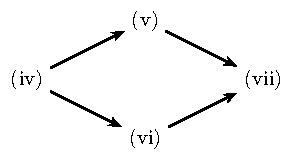
\includegraphics[width=0.5\textwidth]{./tikz-images/tikz-chap-a4.pdf}
\end{center}
%% --
If\/ $A$ is a bounded operator, that is, if\/ $D(A) = E$, then
%% --
\[
\text{(iv) $\Leftrightarrow$ (v) and (vi) $\Leftrightarrow$ (vii).}
\]
However, if\/ $A$ is unbounded, all stability notions may differ, as illustrated in the following examples.
%%--
\begin{example}\label{ex:a4-1.2}
\begin{enumerate}[\upshape (i), wide, labelindent=.25em]

\item 
Let $E = c_{0}$. 
Then 
%% --
\[
A \colon (x_{n})_{n \in \N} \mapsto (-1/n \cdot x_{n})_{n \in \N}
\] 
%% --
generates the semigroup 
%% --
\[
T(t)(x_{n})_{n \in \N} = (\eu^{-t/n} x_{n})_{n \in \N}.
\]
%% --
It is easy to see that $\|T(t)\|=1$ and that $\|T(t)f\|\to 0$ for every $f \in c_{0}$.

Moreover, since $A$ is a bounded operator, $D(A) = E$.
This gives an example of a uniformly stable but not exponentially stable semigroup.

The translation semigroups generated by the first derivative on $C_0(\R_{+})$ or $L^{p}(\R_{+})$ for $1 < p < \infty$ offer further examples of (uniformly) stable but not exponentially stable semigroups.

Moreover, as shown in the example before Theorem~\ref{thm:a2-1.14},
the Laplacian $\Delta$ on $C_0(\R^{n})$ generates a bounded holomorphic semigroup given by 
\index{operator!Laplacian}
%% --
\[
T(t)f(x) = (4\pi t)^{-n/2} \int_{\R^{n}} \eu^{-|x-y|^{2}/4t} f(y)  \dy .
\]
%% --
This semigroup is not exponentially stable because $0 \in \sigma(\Delta)$ ($\Im(\Delta) \not= C_0(\R^{n})$); see Corollary~\ref{cor:a4-1.5} below. To see that the semigroup is (uniformly) stable, observe that for every fixed $x\in\R^n$, the kernel 
%
\[
	k_t(x,y) \coloneq  \mleft(4\pi t\mright)^{-n/2} \eu^{-|x-y|^{2}/4t}
\]
%
defines a probability density with $\int_{\R^n} k_t(x,y) \dy\, = 1$. Hence, $\|T(t)\|  \leq 1$; in fact, $\|T(t)\| = 1$ since $k_t$ also forms an approximate identity. Let $f \in C_0(\R^{n})$ and $\epsilon > 0$. Then there exists a compactly supported $g \in C_0(\R^{n})$ such that $\|f-g\|  \leq \epsilon$. Therefore,
%% --
\[
\|T(t)f\|  \leq  \|T(t)\|\|f-g\| + \|T(t)g\|  \leq \epsilon + (4\pi t)^{-n/2} \int_{\R^{n}} |g(y)|  \dy\, ,
\]
%% --
which implies  $\|T(t)f\| \to 0$ as $t\to\infty$ for all $f \in C_0(\R^{n})$; see also Part-II, Example~\ref{ex:b3-1.7}.
%%--
This shows that the Laplacian on $C_0(\R^{n})$ (and also on $L^{p}(\R^{n})$ for $1 < p < \infty$, see 
Example~\ref{ex:a4-15} below) generates a uniformly stable but not exponentially stable semigroup.

\item 
Note that the condition 
%% --
\[
0 \leq \omega_{0}(A) = \inf\{\omega\colon\|T(t)\| \leq M\eu^{\omega t} \text{ for all } t \geq 0\}
\]
%% --
does not exclude the possibility that the semigroup is exponentially stable.

To see this, consider $E \coloneq C_0(\R_{+}) \cap $ $L^{1}(\R_{+},\eu^{x}\dx)$. 
Then, as shown in Example~\ref{ex:a3-1.3} 
the translation semigroup satisfies $\|T(t)\| = 1$, and hence $\omega_{0}(A) = 0$. 
For every $\lambda \in \C$ with $\Re(\lambda) > -1$ and every $f \in E$, the resolvent of the generator is given as $R(\lambda,A)f = \int_{0}^{\infty} \eu^{\lambda t} T(t)f  \dt$.
From Eq.~\myeqpageref{eq:a1-3.2}, it follows that
%% --
\[
T(t)f = \eu^{\lambda t}\left(f - \int_{0}^{t} \eu^{-\lambda s} T(s) (\lambda - A)f  \ds\right),
\]
%% --
and from the existence of the limit
%% --
\[
\lim_{t \to \infty} \int_{0}^{t} \eu^{-\lambda s} T(s) (\lambda - A)f  \ds,
\] 
%% --
it follows that 
$\|T(t)f\| \leq M\eu^{\lambda t}$ for every $f \in D(A)$ and some constant $M$ depending on $f$. This yields $\omega_{1}(A)  \leq -1 < 0 = \omega_{0}(A)$. 
Thus, we have a semigroup that is exponentially stable, but not uniformly exponentially stable.

\item
Rescaling this semigroup (see Section~\ref{subsec:a1-3.2}), we obtain a semigroup with $\omega_{1}(A) = -1/2 $ and $\omega_{0}(A) = 1/2 $.
Therefore, there exist exponentially stable (and hence, stable) semigroups that are not bounded, and hence, not uniformly stable.
This example illustrates that there may be a significant difference between the long-term behavior of the semigroup $(T(t))_{t \geq 0}$ (\ie the set of all mild solutions) and the long-term behavior of the strong solutions $\{T(\cdot)f \colon f \in D(A)\}$ of (ACP). 
\end{enumerate}
\end{example}
%% -- 
In what follows, we characterize the exponential growth bounds $\omega(f)$, $\omega_{1}(A)$, and $\omega_{0}(A)$ in terms of certain abscissas of simple or absolute convergence of the Laplace transform of\/ $T(\cdot)f$. 
These characterizations will serve as one of the tools for 
establishing that, for certain semigroups beyond the class of eventually norm-continuous semigroups (see Theorem~\ref{thm:a3-6.6}), the growth bounds $\omega_{0}(A)$ and/or $\omega_{1}(A)$ coincide with the spectral bound %
\[
	s(A) = \sup\{\Re(\lambda)\colon\lambda \in \sigma(A)\} .
\]
%
For results of this type, see, for example, Part-II, Chapter~\ref{chap:b4},  Part-III, Chapter~\ref{chap:c4},  and Part-IV, Chapter~\ref{chap:d4}.
\index{stability!spectral bound $s(A)$}
\index{spectral bound $s(A)$}


We begin by observing that $s(A)$ can be interpreted as the abscissa of holomorphy of the Laplace transform 
%
\[
	\lambda \mapsto \int_{0}^{\infty} \eu^{-\lambda t} T(t)  \dt 
\]
%
of the semigroup $(T(t))_{t \geq 0}$.
\index{stability!abscissa of holomorphy}
\index{Laplace transform|(} 
Furthermore, we recall that the Laplace transform exists for every $\lambda \in \C$ with $\Re(\lambda) > \Re(\mu)$, provided it exists for some $\mu\in\C$.
This follows from 
%% --
\begin{equation}\label{eq:a4-1.1}
\begin{split}
\int_0^t \eu^{-\lambda s} f(s) \ds &= \eu^{-(\lambda-\mu)t} \int_{0}^{t} \eu^{\mu s} f(s)  \ds \\ 
&+ (\lambda - \mu) \int_{0}^{t} \eu^{-(\lambda-\mu)s} \int_{0}^{s} \eu^{\mu r} f(r) \,\diff{r} \ds  . 
\end{split}
\end{equation}
%% --
Note that even boundedness of 
\[
\left\{ \int_{0}^{t} \eu^{-\mu s}f(s)  \ds \colon t > 0\right\}
\]
%% --
implies the existence of the Laplace transform for $\Re(\lambda) > \Re(\mu)$. 
Therefore, the subset of\/ $\C$ for which the Laplace transform exists is always a half-plane 
%
\[
	\{\lambda \in \C\colon\Re(\lambda)\allowbreak > \gamma\} \cup H , 
\]
%
where $H$ is a subset of the line $\{\lambda \in \C\colon\Re(\lambda) = \gamma\}$.

In the following theorem, we show that the bound of the half-plane for which the Laplace transform of\/ $T(\cdot)f$ ($f \in E$) exists absolutely, and the bound of the half-plane for which the Laplace transform of\/ $T(\cdot)Af$ ($f \in D(A)$) exists strongly, coincide with the growth bound 
%
\[
	\omega(f) = \inf\{\omega\colon\|T(t)f\| \leq M\eu^{\omega t} \text{ for all } t \geq 0\} .
\]
%
%% --
\begin{theorem}\label{thm:a4-1.3}
\index{growth bound!omegaf@$\omega(f)$}
Let $A$ be the generator of a strongly continuous semigroup $ (T(t))_{t \geq 0} $ on a Banach space $E$. 
Then, for every $f \in E$,
%% --
\begin{equation}\label{eq:a4-1.2}
\omega(f) = \limsup_{t \to \infty} \frac{1}{t}\log\|T(t)f\|, 
\end{equation}
%% --
and
%% --
\begin{enumerate}[(i)]
\item 
$\displaystyle\quad
\omega(f) = \inf\{\Re(\lambda)\colon\int_{0}^{\infty} \|\eu^{-\lambda t} T(t)f\|  \dt \text{ exists}\} .$
\end{enumerate}
%% --
If\/ $\ker(A) = \{0\}$, then for every $f \in D(A)$ we have
%% --
\begin{enumerate}[(i), resume]
\item 
$\displaystyle\quad
\,\omega(f) = \inf\{\Re(\lambda)\colon\int_{0}^{\infty} \eu^{-\lambda t} T(t)Af  \dt
\text{ exists}\} .$
\end{enumerate}
%% --
\end{theorem}
%%--
\begin{proof}  The proof of Eq.~\myeqpageref{eq:a4-1.2} is omitted (see \textcite[p.306]{hillephillips:1957}). 
To prove (i) and (ii), we need the following lemma.
%% --
\begin{lemma*}\label{lem:a4-1.3}
Let $F \in C(\R_{+},\R_{+})$ be such that $\int_{0}^{\infty} F(r) \dr$ exists. 
If there exist positive constants $m$ and $n$ such that $F$ satisfies the local growth condition $F(t + s) \leq m \cdot F(s)$ for all $s \geq 0$ and $t \in \left[0,n\right]$, then $\lim_{s \to \infty} F(s) = 0$.
\end{lemma*}
%% --
\begin{proof}
Let $\epsilon > 0$. Since $\int_0^\infty F(r) \dr < \infty$, there exists $a > 0$ such that
\[
A(a) \coloneq \int_{a}^{\infty} F(r) \dr < \frac{n}{m}\epsilon.
\]
Now fix any $s > a + n$. We claim that there exists $r \in [s - n, s]$ such that
\(
F(r) \leq \frac{1}{n}A(a).
\)
Indeed, suppose that $F(r) > \frac{1}{n}A(a)$ for all $r \in [s - n, s]$. Then
\[ 
A(a) = \int_{s-n}^{s}\frac{1}{n}A(a)\dr < \int_{s-n}^{s}F(r)\dr  \leq \int_a^\infty F(r)\dr = A(a) , 
\]
which is a contradiction.
Hence, such an $r \in [s - n, s]$ must exist.
Finally, if\/ $s>a+n$ and $r\in [s-n,s]$, then $0 \leq s-r \leq n$ and, therefore, $F(s) = F(s-r+r) \leq m \cdot F(r) \leq m \cdot \frac{A(a)}{n} < \epsilon$. 
This shows that $\lim_{s \to \infty} F(s) = 0$.
\end{proof}
%% --
To prove part (i) of Theorem~\ref{thm:a4-1.3}, define 
%
\[
	b \coloneq \inf \left\{\Re(\lambda)\colon\int_{0}^{\infty} \|^{-\lambda t} T(t)f\|  \dt \text{ exists} \right\}.
\]
%
A straightforward application of the lemma shows that $\omega(f) \leq b$.
The definition of\/ $\omega(f)$ yields the reverse inequality.

It remains to prove part (ii) of Theorem~\ref{thm:a4-1.3}.
Assume that $\ker(A) = \{0\}$ and let $f \in D(A)$, $\lambda \in \C$ with $\Re(\lambda) > \omega(f)$. 
From the equation
%% --
\[
\int_{0}^{t} \eu^{-\lambda s} T(s)Af  \ds = \eu^{-\lambda t}T(t)f - f + \lambda \int_{0}^{t} \eu^{-\lambda s} T(s)f  \ds
\]
%% --
it follows that $\int_{0}^{\infty} \eu^{-\lambda t} T(t)Af  \dt$ exists. 
Therefore, 
%%--
\[ 
c \coloneq \inf\{\Re(\lambda)\colon\int_{0}^{\infty} \eu^{-\lambda t}T(t)Af  \dt \text{ exists}\} \leq \omega(f) .
\]
%%--
Next, we show that $c < 0$ implies $c = \omega(f)$. 
For $c < 0$, it follows from Eq.~\myeqpageref{eq:a4-1} that $\int_{0}^{\infty} T(s)Af  \ds$ exists. 
Since $\int_{0}^{r} T(s)Af  \ds = T(r)f - f$, it follows that \[g \coloneqq\lim_{r \to \infty} T(r)f\] exists. 
But for every $t \geq 0$, $T(t)g = g$ which implies that $g \in \ker(A) = \{0\}$ or $g = 0$. 
Hence, $\int_{0}^{\infty} T(s)Af  \ds = -f$.

Now, fix $c < r < 0$.
Integrating by parts, we obtain
%% --
%\begin{align*}
%-T(t)f &= \lim_{u \to \infty} \int_{t}^{u} \eu^{r s} \eu^{-r s} T(s)Af  \ds\\
%&= \lim_{u \to \infty} \mleft( \eu^{ru} \int_0^u \eu^{-rs} T(s) Af  \ds 
%	- \eu^{rt} \int_0^t \eu^{-rs} T(s)Af  \ds \\ 
%& \qquad \qquad -r\int_t^u \eu^{rs}\int_0^s \eu^{-rv} T(v)Af \diff{v}  \ds
%\mright) \\
%&= - \eu^{rt}\int_0^t\eu^{-rs} T(s)Af  \ds -r\int_t^\infty \eu^{rs}\int_0^s \eu^{-rv} T(v)Af \diff{v}  \ds.
%\end{align*}
%%% --
\begin{align*}
-T(t)f 
  & = \lim_{u \to \infty} \int_{t}^{u} T(s)Af \diff{s}\\
  & = \lim_{u \to \infty} \Bigl( 
       \eu^{ru} \int_0^u \eu^{-rs} T(s) Af \diff{s} 
     - \eu^{rt} \int_0^t \eu^{-rs} T(s) Af \diff{s} \\
  & \hphantom{{}= \lim_{u \to \infty} \Bigl(}
     {}- r \int_t^u \eu^{rs} \int_0^s \eu^{-rv} T(v) Af \diff{v} \diff{s}
     \Bigr) \\
  & = - \eu^{rt} \int_0^t \eu^{-rs} T(s) Af \diff{s} 
     - r \int_t^\infty \eu^{rs} \int_0^s \eu^{-rv} T(v) Af \diff{v} \diff{s}.
\end{align*}
%% --
From $\left\|\int_{0}^{t} \eu^{-r s} T(s)Af  \ds\right\| \leq M$ for some $M$ and every $t \geq 0$ we conclude that $\|T(t)f\| \leq \tilde{M}\eu^{rt}$ for all $t \geq 0$ and some constant $\tilde{M}$.
Hence, $\omega(f) \leq r$ for every $c < r < 0$, \ie $\omega(f) \leq c$.

If\/ $c \geq 0$ and $w > c$, then $\left\|\int_{0}^{t} \eu^{-w s} T(s)Af \ds\right\| \leq M$ for all $t \geq 0$. 
By 
%% --
\begin{align*}
T(t)f - f & = \int_{0}^{t} \eu^{w s} \eu^{-w s} T(s)Af  \ds\\
& = \eu^{wt}\int_0^t \eu^{-ws} T(s)Af \ds - w\int_0^t\eu^{ws}\int_0^s \eu^{-wr} T(r)Af\, \diff{r} \ds,
\end{align*}
%% --
we obtain $\|T(t)f-f\| \leq M\eu^{w t} + M(\eu^{w t} - 1)
 \leq 2M\eu^{wt}$. 
Hence, $\omega(f) \leq w$ for every $w > c$, that is, $\omega(f) \leq c$.
\end{proof}
%% --
Finally, from Eq.~\myeqpageref{eq:a4-1.2} and the Uniform Boundedness Principle, it follows that the growth bound 
%
\[
	\omega_{1}(A) = \sup\{\omega(f) \colon f \in D(A)\}
\]
%
satisfies
%% --
\begin{equation}\label{eq:a4-1.3}
\begin{split}
\omega_1(A) &={} \inf \{ \omega \colon \text{for every  $f \in D(A)$  there exists a constant $ M $ such that  } \\
& \phantom{xxxxxxxx} \text{ $\|T(t)f\| \leq M\eu^{\omega t}$  for every $t \geq 0$} \} \\
&={}
\limsup_{t \to \infty} \frac{1}{t} \log\|T(t)R(\lambda,A)\| \quad (\lambda \in \rho(A)). 
\end{split}
\end{equation}
%% --
The following theorem plays a central role in the stability theory of positive semigroups.
We show that the constant $\omega_{1}(A)$ coincides both with the abscissa of simple convergence of the Laplace transform of the semigroup and with the abscissa of absolute convergence of the Laplace transform of the strong solutions of (ACP).
%% --
\begin{theorem}\label{thm:a4-1.4}
\index{growth bound!omega1@$\omega_1(A)$}
Let $A$ be the generator of a strongly continuous semigroup $ (T(t))_{t \geq 0} $ on a Banach space $E$. 
Then
%% --
\begin{equation}\label{eq:a4-1.4}
\begin{split}
\omega_{1}(A) = \inf\{\Re(\lambda) &\colon {\int_{0}^{\infty} \eu^{-\lambda t} T(t)f  \dt} \text{\ exists as an\  \ldots }\\
	\phantom{\inf\{\Re(\lambda) \colon exists as an} &\text{\ldots\  improper Riemann integral for every } f \in E\} \\
= \inf\{\Re(\lambda) &\colon {\int_{0}^{\infty} \|\eu^{-\lambda t} T(t)f\|  \dt} \text{ exists for every } f \in D(A)\}.  
\end{split}
\end{equation}
\end{theorem}
%--
\begin{remarks*}\label{rem:a4-1.4}%
%% --
\begin{enumerate}[\upshape (i), wide, labelindent=.25em]

\item 
One can show that the abscissas of uniform, strong, and weak convergence of the Laplace transform coincide (see Part-III, Theorem~\ref{thm:c3-1.2}, last part of the proof). 
Therefore, by Theorem~\ref{thm:a4-1.4},
%--
\begin{equation}\label{eq:a4-1.5}
\begin{split}
\omega_1(A) &= \inf \left\{ \Re(\lambda)\colon\text{weak-} \lim_{t \to \infty} {\int_0^t \eu^{-\lambda s} T(s)  \ds} \text{ exists} \right\} \\
    &= \inf \left\{ \Re(\lambda)\colon\text{uniform-} \lim_{t \to \infty} {\int_0^t \eu^{-\lambda s} T(s)  \ds} \text{ exists} \right\} .
\end{split}
\end{equation}
%% --
\item
In Equations \eqref{eq:a4-1.4} and \eqref{eq:a4-1.5}, the term \enquote{$\Re(\lambda)$} may be replaced by \enquote{$\lambda \in \R$} (use Eq.~\myeqpageref{eq:a4-1}).
\end{enumerate}
%% --
\end{remarks*}
%% --
\begin{proof}(Proof of Theorem~\ref{thm:a4-1.4}) 
The equality 
 \[ 
 \omega_1(A) = \inf \left\{ \Re(\lambda)\colon\int_0^\infty \|\eu^{-\lambda t} T(t) f \|  \dt \text{ exists for all } f \in D(A) \right\} 
 \] 
 follows from the definition of\/ $\omega_1(A)$ and the lemma in the proof of Theorem~\ref{thm:a4-1.3}.
We aim to prove that
\[
\omega_1(A) = \inf \left\{ \Re(\lambda)\colon\int_0^\infty \eu^{-\lambda s} T(s) f  \ds \text{ exists for every } f \in E \right\} \eqqcolon  b. 
\]
The identity
\[
    T(t) f = \eu^{\lambda t} \left\{ f - \int_0^{t} \eu^{-\lambda s} T(s) (\lambda - A) f  \ds \right\}
\]
yields
\[
\omega_1(A) \leq \inf \left\{ \Re(\lambda)\colon\int_0^\infty \eu^{-\lambda t} T(t) f  \dt \text{ exists for every } f \in \Image{\lambda - A} \right\}.
\]
Therefore, $\omega_1(A) \leq b$.
%--
Take $\lambda \in \C$ with $\Re(\lambda) > \omega_1(A)$. 
Then $\int_0^\infty \eu^{-\lambda t} T(t) f  \dt$ exists for every $f \in D(A)$. 

Define 
%
\[
	g \coloneq  \int_0^\infty \eu^{-\lambda t} T(t) f  \dt .
\]
%
Then $g \in D(A)$ and
%
\[
	 \int_0^n \eu^{-\lambda t} T(t) f  \dt = \sum_{k=0}^{n-1} \eu^{-\lambda k} T(k) g .
\]
%
Since $\Re(\lambda) > \omega_1(A)$, the sum converges for every $g \in D(A)$. 
Therefore, the integral converges as $n \to \infty$ for every $f \in E$.

For every $t \in \R_+$, define a bounded operator $T_t$ by $ f \mapsto \int_0^t \eu^{-\lambda s} T(s) f  \ds$. 
As seen above, $T_n f$ converges as $n \to \infty$ for every $f \in E$. 
It follows from the Uniform Boundedness Principle that $(T_n)_{n \in \N}$ is uniformly bounded.

For every $t \in \R_+$, there exist $n \in \N$ and $t' \in [0,1)$ such that $T_t = T_{t'} + \eu^{-\lambda t'} T(t') T_n$. 
Since the operator families on the right side are uniformly bounded, the same is true for $(T_t f)_{t \geq 0}$. 
Since $(T_t f)_{t \geq 0}$ converges for every $f \in D(A)$, it follows that $(T_t f)_{t \geq 0}$ converges for every $f \in E$. 
Thus, $b \leq \omega_1(A)$.
\end{proof}
%% --
%%--
%\medskip
%


The inequality
\[
    \omega_{0}(A) \geq \inf \left\{ \Re(\lambda)\colon\int_0^\infty \|\eu^{-\lambda t} T(t) f \|  \dt 
    \text{ exists for every } f \in E \right\}
\]
combined with the lemma of Theorem~\ref{thm:a4-1.3} implies that the growth bound $\omega_{0}(A)$ coincides with the abscissa of absolute convergence of the Laplace transform of\/ $(T(t))_{t \geq 0}$, \ie
\begin{equation}\label{eq:a4-1.6}
   \omega_{0}(A) = \inf \left\{ \Re  (\lambda)\colon\int_0^\infty \|\eu^{-\lambda t} T(t) f \|  \dt \text{ exists for every } f \in E \right\}.
\end{equation}
%--
%


As seen in Proposition~\ref{prop:a1-1.11}, if\/ $\int_0^\infty \eu^{-\lambda t} T(t) f  \dt$ exists for every $f \in E$, then $\lambda \in \rho(A)$ and $R(\lambda, A) f = \int_0^\infty \eu^{-\lambda t} T(t) f  \dt$. 
This fact and Theorem~\ref{thm:a4-1.4} yield the following corollary.
%--
\begin{corollary} \label{cor:a4-1.5}
\index{stability!spectral bound $s(A)$}
\index{growth bound!omega1@$\omega_1(A)$}
\index{growth bound!omega0@$\omega_0(A)$}
Let $ A $ be the generator of a strongly continuous semigroup $ (T(t))_{t \geq 0} $ on a Banach space $ E $. 
Then  
\[
s(A) \leq \omega_1(A) \leq \omega_{0}(A).
\]
\end{corollary}
%% --
Example~\ref{ex:a4-1.2}\,(ii) shows that uniform exponential stability is not equivalent to 
%
\[
	\sigma(A) \subseteq \{\lambda \in \C \colon \Re(\lambda) \leq q < 0 \} .
\]
%
The following example shows that even strong solutions can be unstable when $ s(A) < 0 $. 
We construct a semigroup where $ s(A) < \omega_1(A) < \omega_{0}(A) $.
%% --
\begin{example}\label{ex:a4-1.6} 
As in Example~\ref{ex:a3-1.4}, consider the semigroup $ (T(t))_{t \geq 0} $ on the Hilbert space $ E = \{(x^1, x^2, ...) \colon x^n \in \C^n\colon\sum_{j=1}^{\infty} \|x^j\|^2 < \infty\} $, defined by 
\[{
T(t) \coloneq  (\eu^{2\pi i n t} \cdot \exp(t A_n))_{n \in \N}
},\]
where
\[
A_n =
\begin{bmatrix}
0 & 1 & 0 & \dots & 0 \\
& 0 & 1 & \dots & 0 \\
& & \ddots & \ddots & \vdots \\
& & & 0 & 1 \\
0 & & & & 0
\end{bmatrix}_{n \times n}.
\]
This semigroup satisfies $ \|T(t)\| = \eu^{t} $ for all $t \geq 0$. Hence, $ \omega_{0}(A) = 1 $, while the generator $ A = (2\pi i n + A_n)_{n \in \N} $ has spectral bound $ s(A) = 0 $. 
We first show that $ \omega_1(A) = \omega_{0}(A) $; this will later be used to construct a semigroup for which $ s(A) < \omega_1(A) < \omega_{0}(A) $. 
Let $ e_n = n^{-1/2} (1, ..., 1) \in \C^n $. 
 
Then, for fixed $n$ and $t \geq 0$, 
%% --  
\begin{align*}
	\|\exp(&t A_n) \cdot e_n\|^2 = \\
	&= \frac{1}{n} \left\| (1 + t + \dots + \frac{t^{n-1}}{(n-1)!}, 1 + t + \dots + \frac{t^{n-2}}{(n-2)!}, \dots, 1+t, 1) \right\|^2 \\
	&=
	\frac{1}{n} \sum_{r=0}^{n-1} \left(\sum_{j=0}^{r} \frac{1}{j!} t^j \right)^2 
	\, = \, \frac{1}{n} \sum_{r=0}^{n-1} \sum_{j,s=0}^{r} \frac{1}{j!s!} t^{j+s} 
	= \frac{1}{n} \sum_{r=0}^{n-1} \sum_{i=0}^{2r} t^i
	\sum_{\substack{j+s=i\\0 \leq j,s \leq r}} \frac{1}{j!\,s!} \\
	& \geq \frac{1}{n} \sum_{r=0}^{n-1} \sum_{i=0}^{r} \frac{(2t)^i}{i!} 
	= \frac{1}{n} \sum_{i=0}^{n-1} (n-i)\,\frac{(2t)^i}{i!} 
	 \geq \frac{1}{n^2} \sum_{i=0}^{n-1} \frac{(2t)^i}{i!}.
\end{align*}
%% --
For $ 0 < q < 1 $, define $ x_q \in E $ as  
$
x_q :=  (q e_1, 2q^2 e_2, ..., n q^n e_n, ...).
$
Then $x_q \in D(A)$ and
%--
\begin{align*}
	\|T(t)x_q\|^2 & = \sum_{n=1}^{\infty} n^2 q^{2n} \| \exp(t A) e_n \|^2
	\geq \sum_{n=1}^{\infty} n^2 q^{2n} \left(\frac{1}{n^2} \sum_{i=0}^{n-1}  \frac{1}{i!} (2t)^i \right)\\
	&= \sum_{i=0}^{\infty} \sum_{n=i+1}^{\infty} \left( q^{2n} \frac{1}{i!} (2t)^i \right)
	= \sum_{i=0}^{\infty} q^{2i+2} (1 - q^2)^{-1} \frac{1}{i!} (2t)^i \\
	&= \frac{q^2}{1 - q^2} \sum_{i=0}^{\infty} \frac{1}{i!} (2t q^2)^i
	= \frac{q^2}{1 - q^2} \eu^{2t q^2}.
\end{align*}
%% -- \noindent kann man sich ersparen, wenn man nach \end{} keine Leerzeile macht, also
%% -- und kein eingerücktes It
It follows that $\omega(x_q) \geq q^2$. 
Thus,
\[
1 = \sup \{\omega(x_q)\colon0 < q < 1\} \leq \omega_1(A) \leq \omega_{0}(A) = 1.
\]
%% --
Rescaling the semigroup (\ie looking at $\eu^{-3/2 \cdot t} T(t)$), we obtain a semigroup generator $A$ on the Hilbert space $E$ with $-3/2 = s(A)$ and $\omega_1(A) = \omega_{0}(A) = -1/2$. 
On the other hand, Example~\ref{ex:a4-1.2}\,(ii) produces a semigroup in a Banach space $F$ with generator $B$ such that $-1 = s(B) = \omega_1(B)$ while $\omega_{0}(B) = 0$. 
Now the operator $C \coloneq  A \oplus B$ on the Banach space $E \oplus F$ is a semigroup generator for which
%% --
\begin{align*}
s(C) &= \max \{s(A), s(B)\} = -1, \quad \omega_1(C) = \max\{\omega_1(A), \omega_1(B)\} = -1/2 \\
& \text{and \phantom{x}} \omega_{0}(C) = \max\{\omega_{0}(A), \omega_{0}(B)\} = 0.
\end{align*}
%% --
\end{example}
%% -- 
\begin{remark}\label{rem:a4-1.7}
For eventually norm continuous semigroups---particularly compact, differentiable, holomorphic, or nilpotent ones--- the spectral mapping theorem 
%% --
\begin{equation}\label{eq:a4-1.7}
\sigma(T(t)) \setminus \{0\} = \eu^{t \sigma(A)}
\end{equation}
%% --
holds. 
Consequently,
%% --
\begin{equation}\label{eq:a4-1.8}
s(A) = \omega_1(A) = \omega_{0}(A)
\end{equation}
%% --
is valid (Corollary~\ref{cor:a4-1.5} and Corollary~\ref{cor:a3-6.7} ).
Hence, if\/ $A$ is the generator of an eventually norm-continuous semigroup, the exponential growth bounds of the strong and mild solutions of the abstract Cauchy problem $\dot{u}(t) = A u(t), u(0) = x$, are determined by the spectral bound
$s(A) = \sup\{\Re(\lambda)\colon\lambda \in \sigma(A)\}.$
\end{remark}
%--
\begin{remark} In general, the growth bound $\omega_{0}(A)$ can be obtained using the Hille-Yosida theorem (see Theorem~\ref{thm:a2-1.7} ) as
%% --
\begin{equation}\label{eq:a4-1.9}
\begin{split}
%% --
\omega_{0}(A) = \inf \{ w\colon\|R(\lambda, A)^n\| \leq &M ( \Re(\lambda) - w)^{-n} \text{ for some } M \text{ and}\\
&\text{every } n \in \N \text{ and } \lambda \in \C \text{ with } \Re(\lambda) > w\}. 
\end{split}
\end{equation}
\index{growth bound!omega0@$\omega_0(A)$}
%% --
Due to the difficulty of estimating all powers of the resolvent, this characterization is of limited practical use. 
\index{resolvent}
However, if\/ $A$ is the generator of a semigroup on a Hilbert space $H$, then it is shown in Corollary~\ref{cor:a3-7.11}  that
%--
\begin{equation}\label{eq:a4-1.10}
 \omega_{0}(A) = \inf \{ w\colon\| R(\lambda, A) \| \leq M_w \quad \text{for } \Re(\lambda) > w \}.
\end{equation}
\end{remark}
%% --
Unfortunately, the identity \myeqpageref{eq:a4-1.10} does not hold on arbitrary Banach spaces. 
However, as we will see in Part-III, Section~\ref{sec:c4-1},  the identity 
%--
\begin{equation}\label{eq:a4-1.11}
 s(A)=\omega_1(A) = \inf \{ w\colon\| R(\lambda, A) \| \leq M_w \quad \text{for } \Re(\lambda) > w \}
\end{equation}
%% --
holds for every positive semigroup on a Banach lattice. 
Consequently, for positive semigroups with $s(A) = \omega_1(A) < \omega_{0}(A)$ (see Example~\ref{ex:a4-1.2}\,(ii)), the identity \myeqpageref{eq:a4-1.10} is not applicable. 
Nevertheless, we can establish the following theorem.
%% --
\begin{theorem}\label{thm:a4-1.9}
\index{growth bound!omegaf@$\omega(f)$}
Let $A$ be the generator of a strongly continuous semigroup $(T(t))_{t \geq 0}$ on a Banach space $E$. 
Suppose there exist constants $a \geq 0$ and $q \geq s(A)$, and constants $C > 0$ and $n \in \N$ such that 
%% --
\[
    \| R(\lambda, A) \| \leq C | \lambda |^{n-2}
\]
%% --
for all $\lambda \in \C$ with $\Re(\lambda) > q$ and $| \Im(\lambda) | > a$. 
Then
%% --
\[
    \sup \{ \omega(f),  f \in D(A^n) \} \leq q.
\]
\end{theorem}
%% -- 
\begin{proof} 
The hypothesis $\| R(\lambda, A) \| \leq C | \lambda |^{n-2}$ is invariant under rescaling. 
That is, the resolvent $R(\lambda, -b+A)$ of the generator $-b+A$ of the rescaled semigroup $\eu^{-bt} T(t)$ satisfies
$\| R(\lambda, -b+A) \| \leq \tilde{C} | \lambda |^{n-2}$ for every $\lambda \in \C$ with $\Re(\lambda) > q-b$ and $| \Im(\lambda) | > a+2b$, for a suitable constant $\tilde{C}$. 
Therefore, we may assume, without loss of generality, that $b \coloneq  \max(\omega_{0}(A), q) < 0$. 

Let $\omega_{0}(A) < p < 0$, and set $p' \coloneq  \max\{p, q\} < 0$. 
Then, for every $f \in D(A)$ , the inversion formula for the Laplace transform yields 
\begin{equation} \label{eq:a4-1.12}
T(t) f = \frac{1}{2\pi i} \int_{p' - i\infty}^{p' + i\infty} \eu^{\lambda t} R(\lambda, A) f \, d\lambda.
\end{equation}
%% --
 (For a proof of the vector-valued inversion formula, see \textcite[p.66]{widder:1946}; see also the notes in this section.)
Using the resolvent equation, we obtain 
\index{resolvent equation}
%% --
\[ 
R(\lambda, A)^n R(0, A) = \sum_{k=1}^{n} (-1)^{k+1} \lambda^{-k} R(0, A)^{n+1-k} + (-1)^n \lambda^{-n} R(\lambda, A).
\]
%% --
Since 
$ \frac {1}{2\pi i} \int_{p' - i\infty}^{p' + i\infty} \eu^{\lambda t} \, \lambda^{-k} \, d\lambda = 0 $ for $ k \geq 1, p' < 0 $ and $ t > 0$, it follows that
 \begin{equation}\label{eq:a4-1.13}
   T(t) R(0, A)^n f = (-1)^n \frac{1}{2\pi i} \int_{p' - i\infty}^{p' + i\infty} \eu^{\lambda t} \lambda^{-n} R(\lambda, A) f \, d\lambda
    \end{equation}
    
 for every $f \in E$ and $t > 0$.
    
 If\/ $q < p'$, then by Cauchy's Integral Theorem and the growth bound $\| R(\lambda, A) \| \leq C | \lambda |^{n-2}$, we can shift the path of integration to 
 $\Re(\lambda) = q$, yielding
 %% --
\[
    T(t) R(0, A)^n f = (-1)^n \frac{1}{2\pi i} \int_{q - i\infty}^{q + i\infty} \eu^{\lambda t} \lambda^{-n} R(\lambda, A) f \, d\lambda.
\]
%% -- 
Thus, we estimate  
\[
\| T(t) R(0,A)^n f \| \leq c' \eu^{q t} \| f \| \int_{-\infty}^{\infty} (q^2 + s^2)^{-1}\ds = M \eu^{q t} \| f \|.
\]
%% --
Equivalently,
%% --
\begin{equation*}
\| T(t) f \| \leq M \eu^{q t} \| A^n f \| \text{ for $f \in D(A^n)$.}
\qedhere
\end{equation*}
\end{proof}
%% --
In view of the characterizations given in Section~\ref{sec:a2-1},  the semigroups considered in the theorem above are holomorphic if\/ $ n = 1 $. 
In this case, one may apply Eq.~\eqref{eq:a4-1.7} on p.~\pageref{eq:a4-1.7} to obtain the stronger statement Eq.~\eqref{eq:a4-1.8}
on the same page.%\marginpar{ulgr: on the same page}

Rather than imposing conditions on the resolvent of\/ $ A $, we now adopt a different perspective and characterize the property \enquote{$ \omega_{0}(A) < 0 $} directly in terms of the semigroup $ (T(t))_{t \geq 0} $.
%% --
\begin{proposition} \label{prop:a4-1.10} 
\index{growth bound!omega0@$\omega_0(A)$}
Let $ A $ be the generator of a strongly continuous semigroup $ (T(t))_{t \geq 0} $ on a Banach space $E$. 
Then the following statements are equivalent.
\begin{enumerate}[\upshape (a)]
\item  
$ \omega_{0}(A) < 0 $.
\item  
$ \lim_{t \to \infty} \| T(t) \| = 0 $.
\item  
$ \| T(t') \| < 1 $ for some $ t' > 0 $.
\end{enumerate}
\end{proposition}
%% --
\begin{proof}
The implications $(a)  \Rightarrow  (b)  \Rightarrow  (c) $ are immediate. To prove $(c)  \Rightarrow  (a) $, note that $\omega_{0}(A) = \lim_{t \to \infty} \frac{1}{t} \log \| T(t) \|$ (see Eq.~\myeqpageref{eq:a1-1.1}). Assume $\|T(t')\| <1$ for some $t'>0$. For $t=nt'+s$ with $s\in [0,t']$, we have $\|T(t)\| \leq \|T(t')\|^n\|T(s)\|$, so that
\[
\displaystyle
\frac{\log \|T(t)\|}{t} \leq \frac{n\log \|T(t')\|}{nt'+s} + \frac{\log \|T(s)\|}{nt' + s}.
\]
Since $\|T(s)\|$ is bounded on compact intervals, the second term tends to zero as $n\to\infty$. The first term tends to 
%
\[
	\frac{\log \|T(t')\|}{t'} < 0 .
\]
%
Thus, $\omega_0(A) < 0$, which proves  $(c)  \Rightarrow  (a) $.
\end{proof}
%% --
Other less obvious characterizations of the property 
\enquote{$ \omega_{0}(A) < 0 $} are provided in the following theorem. 
The equivalence of (a) and (c) is known as \emph{Datko’s Theorem}.
\index{Datko's theorem}
%% -- 
\begin{theorem} \label{thm:a4-1.11} 
\index{growth bound!omega0@$\omega_0(A)$}
\index{stability!spectral bound $s(A)$}
\index{stability!Datko's theorem}
Let $ A $ be the generator of a strongly continuous semigroup $ (T(t))_{t \geq 0} $ on a Banach space $ E $. 
Then the following statements are equivalent.
%% --
\begin{enumerate}[\upshape (a)]
\item
$ \omega_{0}(A) < 0 $.
\item
$ s(A) < 0 $ and there is $ t_0 > 0 $ such that  
$ |\lambda| < 1$ for every $ \lambda \in A\sigma (T(t_0)).$
\item
For some (equivalently, every) $ p \geq 1 $ the integral $ \int_{0}^{\infty} \| T(t) f \|^p\dt $ exists for every $ f \in E $.
\end{enumerate}
\end{theorem}
%% --
\begin{proof} The implication ``(a) $ \Rightarrow $ (b)'' follows from the fact that $ r(T(t)) = \eu^{\omega_{0}(A) t} < 1 $ and $ s(A) \leq \omega_{0}(A) < 0 $. For the point and residual spectrum, the spectral mapping theorem is valid (see Theorem~\ref{thm:a3-6.3} ). Since the approximate point spectrum is closed, the additional assumption in (b)
implies that $ |\lambda| \leq r < 1 $ for all $ \lambda \in A\sigma(T(t_0)) $. 
Consequently, 
%% --
\[
\exp(\omega_{0}(A) \cdot t_0) = r(T(t_0)) \leq \max\{\exp(t_0 \cdot s(A)), r\} < 1,
\]
%% --
which implies $ \omega_{0}(A) < 0 $. 
This proves \textquotedblleft (b) $\Rightarrow$ (a)\textquotedblright. 
For a proof of the equivalence of (a) and (c), we refer to \textcite{datko:1972} or \textcite[Theorem~4.4.1]{pazy:1983}. 
\end{proof}
%% --
By rescaling a given semigroup $ (T(t))_{t \geq 0} $, one obtains the following corollary from Eq.~\myeqpageref{eq:a4-1.1} and statement (c) of the preceding theorem.
%% --
\begin{corollary} \label{cor:a4-1.12} 
Let $ (T(t))_{t \geq 0} $ be a strongly continuous semigroup on a Banach space $ E $. Then the set of\/ $ \lambda \in \C$ for which
\[
\int_{0}^{\infty} \|\eu^{-\lambda t} T (t) f \|  \dt 
\]
exists for every $ f \in E $  is an open right half-plane.
\end{corollary}
%% --
In the next theorem, we present two necessary conditions for the stability of the semigroup $ (T(t))_{t \geq 0} $ in terms of its generator $ A $. 

We will see in Part-III, Chapter~\ref{chap:c4} that for positive semigroups a condition similar to statement (ii) below is even sufficient for stability. 

It is important to note  that stable semigroups need not be uniformly bounded (see Example~\ref{ex:a4-1.2}\,(iii)) and that the equality $ s(A) = \omega_{0}(A) = 0 $ does not imply boundedness or even stability of the semigroup (see also Example~\ref{ex:a1-1.4}\,(i)).
%% --
\begin{theorem} \label{thm:a4-1.13} 
\index{stability!stable}
Let $ A $ be the generator of a stable semigroup $ (T(t))_{t \geq 0} $ on a Banach space $ E $. Then the following assertions hold.
%% --
\begin{enumerate}[\upshape (i)]
    \item 
    $ s(A) \leq 0 $ and $ \Re(\lambda) < 0 $ for every $ \lambda \in P\sigma (A) \cup R\sigma(A) $.
    
    \item 
    $ \lim_{\lambda \downarrow 0} \lambda R(\lambda, A) f $ exists for every $ f \in D(A) $.
\end{enumerate}
\end{theorem}
%% --
\begin{proof} (i) If\/ $ (T(t))_{t \geq 0} $ is stable, then $ \|T(t) f\| \leq M_f $ for every $ f \in D(A) $. Therefore, $ s(A) \leq \omega_1(A) \leq 0 $. 

Assume, by contradiction, that there exists $ \lambda \in P\sigma(A) $ with $ \Re(\lambda) = 0 $. 
Then, by Corollary~\ref{cor:a3-6.4} , there exists $ g \neq 0 $ such that $ T(t) g = \eu^{\lambda t} g $ for all $ t \geq 0 $. Since $ |\eu^{\lambda t}| = 1 $, this contradicts the stability of the semigroup. 

Now assume there exists $ \lambda \in R\sigma(A) = P\sigma(A') $ with $ \Re(\lambda) = 0 $. 
Then there exists $ 0 \neq \phi \in E' $ with $ T(t)^* \phi = \exp(\lambda t) \phi $ for all $ t \geq 0 $. Choose $ f \in D(A) $ such that $ \langle f, \phi \rangle \neq 0 $. 
Then $ |\langle T(t) f, \phi \rangle| = | \langle f, \phi \rangle| > 0 $ for every $ t \geq 0 $, which again contradicts the stability of the semigroup.

(ii) From the stability of the semigroup and the identity   $\int_{0}^{t} T(s) A f  \ds = T(t) f - f$, it follows that  
$\int_{0}^{\infty} T(s) A f  \ds$ exists for every $ f \in D(A) $.  
Since $ \omega_1(A) \leq 0 $, we may apply Theorem~\ref{thm:a4-1.4} to write  $ R(\lambda, A) A f = \int_{0}^{\infty} \eu^{-\lambda s} T(s) A f  \ds $ for every $ \lambda > 0 $. 
By a classical theorem of Laplace transform theory, (for a proof of the vector-valued version one may follow \textcite[p.196]{widder:1971}), we conclude that $\lim_{\lambda \to 0+} R(\lambda,A)Af$ exists
and is equal to $\int_{0}^{\infty} T(s)Af  \ds$. 
The identity $R(\lambda,A)Af = \lambda R(\lambda,A)f - f$
yields the existence of\/ $\lim_{\lambda \to 0+} \lambda R(\lambda,A)f$ for every $f \in D(A)$.
\end{proof}
\index{Laplace transform|)} 

%%--
Bounded holomorphic semigroups (see Definition~\ref{def:a2-1.11}) satisfy the estimate
\[\|AT(t)\| \leq \frac{m}{t}\]
(see \textcite[p.33]{goldstein:1985a}), and hence $T(t)f \to 0$ as $t \to \infty$
for every $f \in \Image{A}$. 
If\/ $\Image{A}$ is dense (\ie $0 \not\in R\sigma(A)$), then we obtain
uniform stability and the following corollary.
%% --
\begin{corollary}\label{cor:a4-1.14}
\index{stability!uniformly stable}
Let $A$ be the generator of a bounded holomorphic
semigroup $(T(t))_{t \geq 0}$ on a Banach space $E$. 
Then the following statements are equivalent.
%% --
\begin{enumerate}[\upshape (a)]
\item 
$0 \not\in P\sigma(A) \cup R\sigma(A)$.

\item 
$(T(t))_{t \geq 0}$ is uniformly stable.

\end{enumerate}
\end{corollary}
%% --
\begin{example}\label{ex:a4-15}
The Laplacian $\Delta$ generates a bounded holomorphic semigroup on $L^{p}(\R^{n})$ for $1 \leq p < \infty$ (see the example preceding
Corollary~\ref{cor:a2-1.13} ).
\index{operator!Laplacian}
All solutions of the equation $\Delta f = 0$ are either constant
or unbounded, so $0 \not\in P\sigma(\Delta)$. 
If\/ $1 < p < \infty$, then the adjoint
of the Laplacian on $L^{p}(\R^{n})$ is the Laplacian on $L^{q}(\R^{n})$, where
$\frac{1}{p} + \frac{1}{q} = 1$. 
Therefore, $0 \not\in P\sigma(\Delta) \cup R\sigma(\Delta)$, and by Corollary~\ref{cor:a4-1.14},
the Laplacian generates a uniformly stable semigroup on  $L^{p}(\R^{n})$
for $1 < p < \infty$. However, since $\Image{ \Delta} \not= L^{p}(\R^{n})$, Corollary~\ref{cor:a4-1.5} implies that the semigroup is not exponentially stable. %\qed
\end{example}
%%--
As seen in Theorem~\ref{thm:a4-1.4}, exponential stability can be characterized by the condition that the abscissa of convergence of the Laplace transform of\/ $(T(t))_{t \geq 0}$ is less than zero. 
This should be compared to the following result, which characterizes (uniform) stability in terms of integrability and the kernel of the generator.
%% --
\begin{theorem}\label{thm:a4-1.16}
\index{stability!stable}
Let $A$ be the generator of a strongly continuous semigroup $(T(t))_{t \geq 0}$ on a Banach space $E$. 
The following assertions are equivalent.
%% --
\begin{enumerate}[\upshape (a)]
\item 
$(T(t))_{t \geq 0}$ is stable.

\item 
$\ker(A) = \{0\}$ and $\int_{0}^{\infty} T(t)f  \dt$ exists for all $f \in \Image{A}$.

\end{enumerate}
%% --
Furthermore the following statements are equivalent,
%% --
\begin{enumerate}[(a')]
\item $(T(t))_{t \geq 0}$ is stable and bounded.
\item $(T(t))_{t \geq 0}$ is uniformly stable.
\item $(T(t))_{t \geq 0}$ is bounded and there is a dense subspace $D$ such that $\int_{0}^{\infty} T(t)f  \dt$ exists for every $f \in D$.
\end{enumerate}
\index{stability!uniformly stable}
\end{theorem}
%% --
\begin{proof}
If\/ $(T(t))_{t \geq 0}$ is stable, then by Theorem~\ref{thm:a4-1.13}, $\ker(A) = \{0\}$, and
\[{
\int_{0}^{t} T(s)Af  \ds = T(t)f - f \to -f \ \text{as} \ t \to \infty .
}\]
Hence, $(a) \Rightarrow (b)$.

Conversely, suppose $\int_{0}^{t} T(s)Af  \ds$ converges as $t \to \infty$. Then, by
the identity above, the limit $g \coloneq \lim_{t \to \infty} T(t)f$ exists. 
Since $\ker(A) = \{0\}$, it follows that $g = 0$, so $T(t)f \to 0$. 
Thus, $(b) \Rightarrow (a)$.

The implication $(a') \Rightarrow (b')$ is immediate. 

If\/ $T(t)f \to 0$ for every $f \in E$, then $\|T(t)\| \leq M$, and $0 \not\in R\sigma(A)$ by Theorem~\ref{thm:a4-1.13}. 
Therefore,
$D \coloneq \Image{A}$ is dense in $E$, and for every $f \in D$, the integral $\int_{0}^{\infty} T(t)f  \dt$ exists. 
This proves $(b') \Rightarrow (c')$. 

It remains to prove $(c') \Rightarrow (a')$.
Define 
%% --
\[
G \coloneq \{h \in E \colon h = \int_{0}^{\infty} T(t)g  \dt \ \text{ for some } \ g \in D\}.
\] 
%% --
We claim that $G$ is dense in $E$. 
Indeed, for any $g\in D$ and $s>0$,  $g - T(s)g \in D$.
Define 
%
\[
	h_{s} = \frac{1}{s} \int_{0}^{\infty} T(t)(g - T(s)g)  \dt = \frac{1}{s} \int_{0}^{s} T(t)g  \dt .
\]
%
Then $h_{s} \in G$, and $h_{s} \to g$ as $s \to 0$. 
Therefore, $D \subseteq \overline{G}$ or $\overline{G} = E$ since $D$ is dense in $E$. 

Now, let $h \in G$, so $h=\int_0^\infty T(t)g\dt$ for some $g\in D$.
Then %
\[
	T(t)h = T(t) \int_{0}^{\infty} T(s)g  \ds = \int_{t}^{\infty} T(s)g  \ds \to 0 
\]
%
as $t \to \infty$.
Since $\|T(t)\| \leq M$, it follows that   $T(t)f \to 0$ for every $f \in E$.
\end{proof}
%% --
\begin{remark}\label{rem:a4-1.17}
\begin{enumerate}[\upshape (i), wide, labelindent=.25em]
\item 
If\/ $A$ is the generator of a stable semigroup
$(T(t))_{t \geq 0}$ on a Banach space $E$, then by the previous theorem,
\[{
\Image{A} \subseteq \left\{f \in E\colon\int_{0}^{\infty} T(t)f  \dt 
\text{ exists} \right\}  \eqqcolon  H .
}
\]
If\/ $g \in H$, then $\int_{0}^{\infty} T(t)g  \dt \in D(A)$ and $A \int_{0}^{\infty} T(t)g  \dt = -g$. 
Thus, $g \in \Image{A}$, and  the dense subspace $\Image{A}$ is given
by
\begin{equation}\label{eq:a4-1.14}
\Image{A} = \left\{f \in E\colon\int_{0}^{\infty} T(t)f  \dt \text{ exists} \right\}
\end{equation}
whenever $A$ generates a stable semigroup $(T(t))_{t \geq 0}$.

\item 
If\/ $\omega(f) < 0$ for every $f \in D(A)$, then $(T(t))$ is stable, but
might not be exponentially stable if
$0 = \omega_{1}(A) = \sup\{\omega(f) \colon f \in D(A)\}$.
\index{growth bound!omega1@$\omega_1(A)$}
In this case, one can show---via a
proof similar to that of Theorem~\ref{thm:a4-1.4}---that the spectrum $\sigma(A)$ must be contained
in the open left half-plane, \ie $\Re(\lambda) < 0$ for all $\lambda \in \sigma(A)$.

\item 
If one defines a semigroup $(T(t))_{t \geq 0}$ to be weakly stable if
$\langle T(t)f,\phi \rangle \to 0$ as $t \to \infty$ for all $f \in D(A)$ and $\phi \in E'$ or as
weakly uniformly stable if the above holds  for all $f \in E$
and $\phi \in E'$, then Theorems~\ref{thm:a4-1.13} and~\ref{thm:a4-1.16} can be reformulated in a weak form (\ie  replacing stable by weakly stable and \emph{lim} by
\emph{weak-lim}). 
The proofs require only obvious modifications.
If $A$ has a compact resolvent, or if $A$ generates a bounded
holomorphic semigroup, then weak stability implies stability. 
In general, this implication fails; \eg the translation semigroup on
$L^{2}(\R)$ is weakly uniformly stable but not stable (see also Part-II, Example~\ref{ex:b4-1.2}).
\end{enumerate}
\end{remark}
\index{stability|)}
%% --
%% --
\section{Stability: Inhomogeneous Case}\label{sec:a4-2}
\index{Cauchy problem!inhomogeneous|(}
\index{stability|(}
%% --
Using the results of the previous section, we now investigate the long-term behavior of solutions to the inhomogeneous initial value
problem
\begin{equation}\label{eq:a4-2.1}
\dot{u}(t) = Au(t) + F(t) \quad , \quad u(0) = f,
\end{equation}
where $A$ generates a strongly continuous semigroup on a
Banach space $ E $ and $F(\cdot)$ is a locally integrable function from $\R_{+}$
into $ E $, referred to as the \emph{forcing term}. 
A function $u(\cdot)$ is called a \emph{(strong) solution} of Eq.~\myeqpageref{eq:a4-2.1}, if\/ $u(\cdot) \colon \R_{+} \to D(A)$, 
$u(\cdot) \in C^{1}(\R_{+},E)$, and Eq.~\myeqpageref{eq:a4-2.1} holds for all $t \geq 0$.
The assumption that $A$ generates a semigroup $(T(t))_{t \geq 0}$
guarantees uniqueness of the solution to Eq.~\myeqpageref{eq:a4-2.1}. 
If\/ $u(\cdot)$ is a solution, then for fixed $t>0$, the function $v(s) \coloneq  T(t-s)u(s)$, $0 \leq s \leq t$, is
differentiable and $v'(s) = T(t-s)F(s)$. 
Since $F(\cdot)$ is locally integrable, it follows that 
%% --
\[
\int_{0}^{t} T(t-s)F(s)  \ds = v(t) - v(0) = u(t) - T(t)f.
\]
%% --
Thus, the solution $u(t)$ of Eq.~\myeqpageref{eq:a4-2.1} is given by
%% --
\begin{equation}\label{eq:a4-2.2}
u(t) = T(t)f + \int_{0}^{t} T(t-s)F(s)  \ds .
\end{equation}
%% --
%%%

%% --
\begin{example*} \label{ex:a4-2.1}
Let $(T(t))_{t \geq 0}$ be a semigroup that is not eventually differentiable. 
Then there
exists $g \in E$ such that $t \mapsto T(t)g$ is not differentiable on $(0,\infty)$.
Consider the initial value problem $\dot{u}(t) = Au(t) + T(t)g$, $u(0) = 0$. This problem has no
(strong) solution $u(\cdot)$, because otherwise we would have 
\begin{align*}
u(t) = \int_{0}^{t} T(t-s)T(s)g  \ds = tT(t)g,
\end{align*}
which would imply that $t\to T(t)g$ is 
differentiable on $\R_{+}$, a contradiction. 
%\qed
\end{example*}
%%%


Whenever the expression Eq.~\myeqpageref{eq:a4-2.2} is well-defined, we refer to it as a  \emph{generalized} (or
\emph{mild}) solution of Eq.~\myeqpageref{eq:a4-2.1}. 
If\/ $F(\cdot)$ is continuous and $f \in D(A)$, then
the generalized solution of Eq.~\myeqpageref{eq:a4-2.1} is a strong solution if and only if the function 
$v(t) \coloneq  \int_{0}^{t} T(t-s)F(s)  \ds$ is differentiable (see \textcite[Chapter~4,2.4]{pazy:1983}). 
There are several sufficient conditions on the generator $A$,
the forcing term $F(\cdot)$, or the space $E$ under which every mild solution
is a strong solution of Eq.~\myeqpageref{eq:a4-2.1} (see \textcite{travis:1981}
or  \textcite[Section~4.2]{pazy:1983}).

%%%
Our aim in this section is to study the asymptotic behavior of the solutions of Eq.~\myeqpageref{eq:a4-2.1} as $t \to \infty$. 
To that end, we consider absolutely integrable or periodic forcing terms $F(\cdot)$, and assume that the semigroup
is uniformly stable.

Similar results for integrable and convergent forcing terms $F(\cdot)$ can
be obtained under the assumption of uniform stability (see \textcite[p.119]{pazy:1983} or \textcite{neubrander:1985b}). 
However, if the
semigroup is positive, these results remain valid even under the weaker assumption of stability (see Part-III, Chapter~\ref{chap:c4}).
Recall from Theorem~\ref{thm:a4-1.13}\,(i) that for stable
semigroups, the range $\Image{A}$ is dense in $E$.
%% --
\begin{theorem}\label{thm:a4-2.1}
\index{stability!absolutely integrable forcing term}
Let $A$ be the generator of a uniformly stable semigroup
$(T(t))_{t \geq 0}$ on a Banach space $E$. 
If there exists $g \in \Image{A}$ such that
$\int_{0}^{\infty} \|F(s) - g\|  \ds < \infty$, then every generalized solution $u(\cdot)$ of
Eq.~\myeqpageref{eq:a4-2.1} converges as $t \to \infty$, and $\lim_{t \to \infty} u(t) = -h$, where $h \in D(A)$ satisfies
$Ah = g$.
\end{theorem}
%% --
\begin{proof}
If\/ $u(\cdot)$ is a generalized solution of Eq.~\myeqpageref{eq:a4-2.1}, then by Eq.~\myeqpageref{eq:a4-2.2}, we have
\[
u(t) = T(t)f + \int_{0}^{t} T(s)g  \ds + \int_{0}^{t} T(t-s)(F(s)-g)  \ds.
\]
By uniform
stability and the identity $\int_0^t T(s)Ah \ds = T(t)h - h$ (see Theorem~\ref{prop:a1-1.6}), the first term converges to zero
and the second term converges to $-h$. 
It remains to show that the
third term also converges to zero. 
Let $\epsilon > 0$ and define $G(s) \coloneq F(s)-g$. 
Then for any $r>0$,
\begin{align*}
\left\|\int_{0}^{t} T(t-s)G(s)  \ds\right\| & 
{\leq \left\|\int_{0}^{r} T(t-r+r-s)G(s)  \ds\right\| + \left\|\int_{r}^{t} T(t-s)G(s)  \ds\right\|}\\
& 
{\leq \left\|T(t-r)\int_{0}^{r} T(r-s)G(s)  \ds\right\| + M \int_{r}^{\infty} \|G(s)\|  \ds\,},
\end{align*}
where $\|T(t)\| \leq M$ for all $t \geq 0$. Since the semigroup is uniformly stable, we obtain
$T(t-r)\int_{0}^{r} T(r-s)G(s)  \ds \to 0$ as $t \to \infty$ for every $r \geq 0$.
Therefore, $\|\int_{0}^{t} T(t-s)G(s)  \ds\| \leq \epsilon$ for all sufficiently large $t$.
\end{proof}
%% --

In the following theorem, we show that if $A$ generates a
uniformly stable semigroup, the forcing term $F(\cdot)$ is $p$-periodic
and $\int_{0}^{p} T(p-s)F(s)  \ds \in \Image{\Id - T(p)}$, then Eq.~\myeqpageref{eq:a4-2.1}
 admits a unique $p$-periodic mild solution that is \emph{asymptotically stable}; 
 \index{stability!asymptotically stable}\ie for every generalized solution $v(\cdot)$ of Eq.~\myeqpageref{eq:a4-2.1}, 
%% --
\[
\lim_{t \to \infty} \|v(t) - u(t)\| = 0.
\]  
(Notice that, by
Theorem~\ref{thm:a4-1.13} and Lemma~\ref{lem:a3-5.3}, $\overline{ \Image{ \Id - T(p) } } = E $.)
%% --
\begin{lemma}\label{lem:a4-2.2}
Let $A$ be the generator of a strongly continuous semigroup $(T(t))_{t \geq 0}$ on a Banach space $E$, and let $F(\cdot)$ be a $p$-periodic, locally integrable function with $p > 0$. 
Then the following statements are equivalent.
%% --
\begin{enumerate}[\upshape (a)]
\item 
$\dot{u}(t) = Au(t) + F(t)$ admits a (unique) generalized $p$-periodic solution.

\item 
There exists a (unique) $f \in E$ such that $(\Id - T(p))f = \int_{0}^{p} T(p-s)F(s)  \ds$.
\end{enumerate}
\end{lemma}
%% --
\begin{proof}
(a) $\Rightarrow$ (b): 
Let $f \coloneq u(0)$ be the initial value for which Eq.~\myeqpageref{eq:a4-2.1} admits a $p$-periodic mild solution. 
Then for every $t \geq 0$,
%% --
\begin{align*}
u(t) &= u(t+p) \\
&= T(t)T(p)f + \int_{0}^{p} T(t+p-s)F(s)  \ds + \int_{p}^{t+p} T(t+p-s)F(s)  \ds \\
&= T(t)\left[T(p)f + \int_{0}^{p} T(p-s)F(s)  \ds\right] + \int_{0}^{t} T(t-s)F(s)  \ds.
\end{align*}
%% --
Since $u(t) = T(t)f+\int_0^t T(t-s)F(s)\ds$, it follows that
\[T(t)f = T(t)\left[T(p)f+\int_0^pT(p-s)F(s)\ds\right].\]
This implies $f = T(p)f + \int_{0}^{p} T(p-s)F(s)  \ds$.
If\/ $u(\cdot)$ is a unique periodic solution with $u(0) = f$, then $f$ is the unique element in $E$ for which this identity holds.

(b) $\Rightarrow$ (a):  
Define $u(\cdot)$ as in Eq.~\myeqpageref{eq:a4-2.2}. 
Then
%% --
\begin{align*}
u(t+p) = T(t)\left[T(p)f + \int_{0}^{p} T(p-s)F(s)  \ds\right] + \int_{0}^{t} T(t-s)F(s)  \ds = u(t).
\end{align*}
%% --
If\/ $f$ is unique, then, by the above considerations, the solution is also unique.
\end{proof}
%% --
\begin{remark}\label{rem:a4-2.3}
Let $A$ be the generator of a strongly continuous semigroup for which the spectral mapping theorem holds (Section~\ref{sec:a3-6}), and let $F$ be a $p$-periodic forcing term.
If\/ $\frac{2\pi in}{p} \in \rho(A)$ for every $n \in \Z$, then, by Lemma~\ref{lem:a4-2.2}, Eq.~\myeqpageref{eq:a4-2.1}
admits a unique $p$-periodic solution with initial value $(\Id - T(p))^{-1} \left(\int_{0}^{p} T(p-s)F(s)  \ds\right)$.
\end{remark}
%% --
As a consequence of Theorem~\ref{thm:a4-1.13}  and Corollary~\ref{cor:a3-6.4},  a uniformly stable semigroup admits at most one $f \in E$ satisfying 
%% --
\[
(\Id-T(p))f = \int_{0}^{p} T(p-s)F(s)  \ds .
\]
%% --
This fact, together with Lemma~\ref{lem:a4-2.2}, is used to prove the following theorem.
%% --
\begin{theorem}\label{thm:a4-2.4}
\index{stability!periodic forcing term}
\index{semigroup!stable semigroup|)}
Let $A$ be the generator of a uniformly stable semigroup $(T(t))_{t \geq 0}$ and let $F(\cdot)$ be a $p$-periodic, locally integrable function such that 
%% --
\[{
(\Id - T(p))f = \int_{0}^{p} T(p-s)F(s)  \ds \ \text{ for some } \ f \in E .
}
\]
%% --
Then the unique $p$-periodic generalized solution
%% --
\[
u(t) = T(t)f + \int_{0}^{t} T(t-s)F(s)  \ds
\]
%% --
is asymptotically stable. 
%% --
\end{theorem}
\index{semigroup!asymptotics|)}
%% --
\begin{example}\label{ex:a4-2.5}
Let $E$ be the Banach space $C_{0}(\R_{+})$ of continuous functions vanishing at infinity.
The operator $A = \frac{d}{dx}$ with domain $D(A) = \{f \in E: f' \in C^{1} \text{ and } f' \in E\}$ is the generator of the uniformly stable translation semigroup $T(t)f(x) \coloneq f(t+x)$. 
Applying Eq.~\myeqpageref{eq:a4-1.14}, we obtain that $\Image{A} = \{f\colon\int_{0}^{\infty} f(x) \,\dx \text{ exists}\}$ is dense in $C_{0}(\R_{+})$. 
Let $r \in \Image{A}$ and let $F(\cdot)$ be a $p$-periodic, real-valued function.
We apply Theorem~\ref{thm:a4-2.4}  to the initial value problem
%% --
\begin{equation}
 \frac{d}{dt} u(t,x) = \frac{d}{dx}u(t,x) + r(x)F(x+t), \quad u(0,\cdot) \in D(A). 
 \tag{*}
\end{equation}
%% --
We rewrite (*) as  
%% --
\begin{equation}
\dot{v}(t) = Av(t) + G(t), \tag{**}
\end{equation}
%% --
where $v(t) = u(t,\cdot)$ and $G\colon\R_{+} \to E$ is defined by $G(t)(x) = r(x)F(x+t)$.
Then $G$ is $p$-periodic with values in $E$ and $h_{0} \coloneq \int_{0}^{p} T(p-t)G(t)  \dt$ is the function 
%
\[
	x \mapsto \left[\int_{0}^{p} T(p-t)G(t)  \dt\right](x) = F(x)\int_{x}^{x+p} r(s)  \ds .
\]
%
Now define $f \coloneq  \sum_{k=0}^{\infty} T(kp)h_{0}$, which corresponds to the function $x \mapsto F(x)\int_{x}^{\infty} r(s)  \ds$. It is then clear that $(\Id - T(p))f = h_{0}$. 
Therefore, (**) admits a unique $p$-periodic generalized solution by Theorem~\ref{thm:a4-2.4}, even though $\im \R \subseteq \sigma(A)$ (\cf Remark~\ref{rem:a4-2.3}).

The unique $p$-periodic generalized solution $u(t,\cdot)$ is given explicitly by 
%% --
\[
u(t,x) = F(x+t)\int_{x+t}^{\infty} r(s) \ds + F(x+t)\int_{x}^{x+t} r(s) \ds = F(x+t)\int_{x}^{\infty} r(s) \ds.
\]
%% --
Finally, for every solution $v(t,\cdot)$ of (*), Theorem~\ref{thm:a4-2.4} implies that
%% --
\[
\sup\left\{\left|v(t,x) - F(x+t)\int_{x}^{\infty} r(s)  \ds\right| \colon x \in \R_{+}\right\} \to 0 \quad \text{as} \quad t \to \infty .
\]
%% --
\end{example}
\index{asymptotic behavior|)}
\index{stability|)}
%% --
%\newpage
\section*{Notes}
\addcontentsline{toc}{section}{Notes}
%\markboth{Notes and References}{Notes and References}
%% --
\begin{enumerate}[label=\emph{Section 4.\arabic*:}, wide, itemsep=1ex]

\item 
The exponential growth bounds $\omega(f)$ and $\omega_{0}(A)$ as well as the characterizations Eq.~\myeqpageref{eq:a4-1.2}, Eq.~\myeqpageref{eq:a4-1.6} and Theorem~\ref{thm:a4-1.3}\,(i) can be found in \textcite{hillephillips:1957}.
Growth bounds similar to $\omega_{1}(A)$ were first considered in \textcite{djacenko:1976} and in \textcite[Proposition~2]{zabczyk:1979}. 
Example~\ref{ex:a4-1.2}(ii) is taken from \textcite{wolff:1981}; other \emph{counterexamples} can be found in \textcite{hillephillips:1957}, \textcite{foias:1973}, \textcite{triggiani:1975a}, 
\textcite{zabczyk:1975} and \textcite{greinervoigtwolff:1981}. 
Statements Eq.~\myeqpageref{eq:a4-1.2}, Eq.~\myeqpageref{eq:a4-1.6} and Theorem~\ref{thm:a4-1.3}\,(i) are semigroup versions of results in classical Laplace transform theory, see \textcite{hillephillips:1957} and \textcite{widder:1946}. 
Theorem~\ref{thm:a4-1.3}\,(ii) is a semigroup version of Theorem 1.2.7 and 1.2.8 in \textcite{doetsch:1950}. 
The lemma in the proof of Theorem~\ref{thm:a4-1.3} is taken from \textcite{milstein:1975}. 
Theorem~\ref{thm:a4-1.4} and Corollary~\ref{cor:a4-1.5} can be found in \textcite{neubrander:1985a}. 
Example~\ref{ex:a4-1.6} follows Remark~2 in \textcite{zabczyk:1975}. 
Statement Eq.~\myeqpageref{eq:a4-1.8} is sometimes called the \emph{spectrum determined growth assumption}, see, for example, \textcite{triggiani:1975b}. 
Theorem~\ref{thm:a4-1.9} is due to \textcite{slemrod:1976}. 
The proof presented here is based on the following sharper version of the inversion formula for the Laplace transform, which improves on the one given in \textcite[p.349]{hillephillips:1957}. 
Using \textcite[p.66]{widder:1946} or \textcite[p.212]{doetsch:1950} one can establish the following theorem (see \textcite{neubrander:1984b}).
%% --
\begin{theorem}\label{thm:a4-2.6}
Let $A$ be the generator of a strongly continuous semigroup $(T(t))_{t \geq 0}$ on a Banach space $E$. 
For every $f \in D(A)$ and $p > \omega_{1}(A)$ we have
%% --
\[
T(t)f = \frac{1}{2\pi i} \int_{p-i\infty}^{p+i\infty} \eu^{\mu t}R(\mu,A)f \, d\mu.
\]
%% --
\end{theorem}
 

The equivalence of the statements Eq.~\myeqpageref{eq:a4-1.12}, Eq.~\myeqpageref{eq:a4-1.13} and \emph{$\omega_{0}(A) < 0$} was observed by many authors, see for example, \textcite[p.178]{balakrishnan:1976}, 
or \textcite{benchimol:1978b}. 
Theorem~\ref{thm:a4-1.11} is due to \textcite{datko:1970};
for a proof see \textcite[p.116]{pazy:1983}. 
Theorems~\ref{thm:a4-1.13} and~\ref{thm:a4-1.16} can be found in \textcite{neubrander:1985b} and Corollary~\ref{cor:a4-1.14} is due to \textcite{komatsu:1969}. 
An example of an unstable semigroup generator $A$ with $\Re(\mu) < 0$ for all $\mu \in \sigma(A)$ is given in \textcite{datko:1983}.

\item For a discussion of well-posedness of inhomogeneous Cauchy problems, we refer to \textcite[p.83]{goldstein:1985a}, and \textcite[p.105]{pazy:1983}. 
Further results on the asymptotic behavior of the solutions of the inhomogeneous problem can be found in \textcite{raohengartner:1974}, \textcite{zaidman:1979}, \textcite{pazy:1983}, and \textcite{neubrander:1985b}. 
Results similar to Lemma~\ref{lem:a4-2.2} and Theorem~\ref{thm:a4-2.4} are due to \textcite{pruess:1984}. 
For a discussion of the asymptotic behavior of the solutions of\/ $\dot{u}(t) = A(t)u(t) + F(t)$ see \textcite{datko:1972} and \textcite[p.172]{pazy:1983}.

\end{enumerate}
\index{Cauchy problem!inhomogeneous|)}
%% --
%% -- References 
%% --
\section*{References}
\addcontentsline{toc}{section}{References}
{\RaggedRight
  \printbibliography[heading=none]
 }

%%% -- Part-B
%% --
\begin{partbacktext}
\part{Positive Semigroups on Spaces \texorpdfstring{$C_{0}(X)$}{C₀(X)}}
%% -- Einleitungstext des Teils (Rückseite des Teil-Titelblatts),
%% -- übernommen aus LN-Contract-Springer/cover-teaser/Teaser.tex, 23.10.2026.
This part focuses on positive semigroups acting on $C_{0}(X)$ spaces, where $X$ is a locally compact space.
Due to their concrete structure as Banach lattices, these spaces provide an accessible and intuitive setting in which many fundamental phenomena of positive semigroups can be studied in detail.
After fixing notation and reviewing the basic properties of $C_{0}(X)$ and $C(K)$, where $K$ is compact, the theory proceeds to characterize positive semigroups, their generators and, as a special case, associated flows.
Spectral and asymptotic properties, including stability, irreducibility and compactness, are covered in depth.
The results in this part serve as both a motivating model and a testing ground for the more abstract theory developed later.
\end{partbacktext}
%\setcounter{chapter}{0}

    % !TEX root = ../LN-Book-New.tex
%% -- Stand: 2026-03-09
%% --
%%\setcounter{section}{0}
%% --
\chapternopage{Basic Results on Spaces \texorpdfstring{$C_{0}(X)$}{C_0(X)}}
\label{chap:b1}%
\thispagestyle{empty}
%% --
{\Large
\vspace*{-.75cm}
by \\[.25em]
Rainer Nagel and Ulf Schlotterbeck
\vspace{.75cm}
\\
}
%% --
This part of the book is devoted to one-parameter semigroups of operators on spaces of continuous functions of type $C_{0}(X)$.
\index{Banach lattice}
These spaces are Banach lattices of a particularly special kind.
We treat this case separately because mixing it with the abstract Banach lattice theory considered in Part-III would obscure the accessibility and exemplary power of the methods and results presented here.
In this chapter we fix the notation we are going to use and collect some basic facts about the spaces we are considering.

If\/ $X$ is a locally compact space, then $C_{0}(X)$ denotes the space of all continuous complex-valued functions on $X$ that vanish at infinity, endowed with the supremum norm.
If\/ $X$ is compact, then any continuous function on $X$ vanishes at infinity, and $C_{0}(X)$ is the space of all continuous functions on $X$.
We often write $C(X)$ instead of\/ $C_{0}(X)$ in this case.

We sometimes study real-valued functions and denote the corresponding spaces as $C_{0}(X,\mathbb{R})$ and $C(X,\mathbb{R})$; we use the notations $C_{0}(X,\mathbb{C})$ and $C(X,\mathbb{C})$ when we need to distinguish between the two cases.
%% --
\section{Algebraic and Order Structure: Ideals and Quotients}\label{sec:b1-1}%
%% --
Any space $C_{0}(X)$ is a commutative \CA-algebra under the sup-norm and the pointwise multiplication, and by the \emph{Gelfand Representation Theorem} any commutative \CA-algebra can, on the other hand, be canonically represented as an algebra $C_{0}(X)$ on a suitable locally compact space $X$.
The algebraic notions of ideal, quotient, homomorphism are well known and need not be explained further.

Another natural and important structure of\/ $C_{0}(X)$ is the \emph{pointwise} ordering under which $C_{0}(X,\R)$ is a (real) Banach lattice and $C_{0}(X,\C)$ a complex Banach lattice in the sense explained in Part-III, Chapter~\ref{chap:c1}.
Concerning the order structure of\/ $C_{0}(X)$ we use the following notations for a function $f$ in $C_{0}(X,\R)$.
%% --
\begin{enumerate}[\upshape (i), labelindent=.25em]
\item
The function $ f $ is called \emph{positive, $ f \geq 0 $,} if\/ $ f(t) \geq 0  $ for all $ t \in X $, 

\item
We write $f>0$ if\/ $ f $ is positive but does not vanish identically,

\item
We call $ f $ \emph{strictly positive, $f \gg 0$,}  if\/ $ f(t) > 0 $ for all $ t \in X $.

\end{enumerate}
%% --
The notion of an order ideal explained in Part-III, Chapter~\ref{chap:c1} applies of course to the Banach lattices $C_{0}(X)$ and might give rise to confusion with the corresponding algebraic notion.

However, since we are mainly considering closed ideals and since a closed linear subspace $J$ of\/ $C_{0}(X)$ is a lattice ideal if and only if\/ $J$ is an algebraic ideal, we may and will simply speak of closed ideals, without specifying whether we think of the algebraic or the order theoretic meaning of this word.

An important and frequently used characterization of these objects is the following: A subspace $J$ of\/ $C_{0}(X)$ is a closed ideal if and only if there exists a closed subset $F$ of\/ $X$ such that a function $f$ belongs to $J$ if and only if\/ $f$ vanishes on $F$.
The set $F$ is of course uniquely determined by $J$ and is called the \emph{support} of\/ $J$.

If\/ $J = J_{F}$ is a closed ideal with support $F$, then $J_{F}$ is naturally isomorphic to $C_{0}(X\backslash F)$ and the quotient $C_{0}(X)/J$ (under the natural quotient structure) is again a Banach algebra and a Banach lattice that can be identified canonically (via the map $f + J \to f\vert_{F}$) with $C_{0}(F)$.
%% --
\section{Linear Forms and Duality}\label{sec:b1-2}%
%% --
The \emph{Riesz Representation Theorem} asserts that the dual of\/ $C_{0}(X)$ can be identified in a natural way with the space of bounded regular Borel measures on $X$.
While there is no natural algebra structure on this dual, the dual ordering (see Part-III, Chapter~\ref{chap:c1}) makes $C_{0}(X)'$ into a Banach lattice.
We will occasionally make use of the order structure of\/ $C_{0}(X)'$, but since at least its measure theoretic interpretation is supposed to be well-known, it may suffice here to refer to Part-III,
%Chapter~\ref{chap:c1},
Sections~\ref{sec:c1-3} and~\ref{sec:c1-7}, for a more detailed discussion.
We recall only some basic notations here.

If\/ $\mu$ is a linear form on $C_{0}(X,\R)$, then
%% --
\begin{enumerate}[\upshape (i), labelindent=.25em]

\item
$ \mu $ is called \emph{positive}, $\mu \geq 0$, if $ \mu(f) \geq 0 $ for all $ f \geq 0 $;  
\item
$ \mu > 0 $ means that $ \mu $ is positive but does not vanish identically,

\item
$ \mu \gg 0 $ means that $ \mu(f) > 0 $ for any $ f > 0 $;  $ \mu $ is then called \emph{strictly positive}.

\end{enumerate}
%% -- 
If\/ $\mu$ is a linear form on $C_{0}(X,\C)$, then $\mu$ can be written uniquely as 
%
\[
	\mu = \mu_{1} + \im \mu_{2}
\]
%
where $\mu_{1}$ and $\mu_{2}$ map $C_{0}(X,\R)$ into $\R$ (decomposition into \emph{real} and \emph{imaginary parts}).

We call $\mu$ \emph{positive} (\emph{strictly positive}) and use the above notations if\/ $\mu_{2} = 0$ and $\mu_{1}$ is positive (strictly positive).
We point out that strictly positive linear forms need not exist on $C_{0}(X)$, but if\/ $X$ is separable, then a strictly positive linear form is obtained by summing a suitable sequence of point measures.

The coincidence of the notions of a closed algebraic and a closed lattice ideal in $C_{0}(X)$ has of course its effect on the algebraic and the lattice theoretic notions of a homomorphism.
The case of a homomorphism into another space $C_{0}(Y)$ will be discussed below.
As for homomorphisms into the scalar field, we have essentially coincidence between the algebraic and the order theoretic meaning of this word, more exactly: 
%% --
\begin{quote}
\emph{A linear form $\mu \neq 0$ on $C_{0}(X)$ is a lattice homomorphism if and only if\/ $\mu$ is, up to normalization, an algebra homomorphism }(algebra homomorphisms $\neq 0$ must necessarily have norm $1$).
\end{quote}
%% --
Since the algebra homomorphisms $\neq 0$ on $C_{0}(X)$ are known to be the point measures (denoted by $\delta_{t}$) on $X$ and, since on the other hand, $\mu$ is a lattice homomorphism if and only if 
\index{lattice homomorphism}
%
\[
	|\mu(f)| =  \mu(|f|) \quad \text{for all $f$,}
\]
%
it follows that this latter condition on $\mu$ is equivalent to $\mu = \alpha\delta_{t}$ for a suitable $t$ in $X$ and a positive real number $\alpha$.

This can be summarized by saying that $X$ can be canonically identified, via the map $t \to \delta_{t}$, with the subset of the dual $C_{0}(X)'$ consisting of the non-zero algebra homomorphisms, which is also the set of all normalized lattice homomorphisms.
This identification is a topological isomorphism with respect to the weak*-topology of\/ $ C_{0}(X)' $.
%% -- 
\section{Linear Operators}\label{sec:b1-3}%
%% --
A linear mapping $T$ from $C_{0}(X,\R)$ into $C_{0}(Y,\R)$ is called
%% --
\begin{enumerate}[\upshape (i), labelindent=.25em]

\item
\emph{positive} (notation: $T \geq 0$)  if\/ $Tf$  is positive whenever $ f $ is positive, 

\item
\emph{lattice homomorphism}  if\/ $|Tf| = T|f|$  for all $ f $,
\index{lattice homomorphism}

\item
\emph{Markov operator}  if  $ X $ and $ Y $ are compact and $ T $ is a positive operator mapping $\1_{X}$ to $\1_{Y}$.
\index{operator!Markov}

\end{enumerate}
%% --
In the case of complex scalars, $T$ can be decomposed into real and imaginary parts.
We call $T$ positive in this situation if the imaginary part of\/ $T$ is $= 0$ and the real part is positive.
The terms \emph{Markov operator} and \emph{lattice homomorphism} are defined as above.
Note that a complex lattice homomorphism is necessarily positive, and that the \emph{complexification} of a real lattice homomorphism is a complex lattice homomorphism.
Positive operators are always continuous.

Note that the adjoint of a Markov operator $T$ maps positive normalized measures into positive normalized measures while the adjoint of an algebra homomorphism (lattice homomorphism) maps point measures into (multiples of) point measures.
Therefore the adjoint of a Markov lattice homomorphism as well as the adjoint of an algebra homomorphism induces a continuous map $\phi$ from $Y$ (viewed as a subset of the weak dual $C(Y)'$) into $X$ (viewed as a subset of\/ $C(X)'$).

This mapping $\phi$ determines $T$ in a natural and unique way, so that the following are equivalent assertions on a linear mapping $T$ from a space $C(X)$ into a space $C(Y)$.
%% --
\begin{enumerate}[\upshape (a)]
\item 
	$T$ is a Markov lattice homomorphism.
\item 
	$T$ is a Markov algebra homomorphism.
\item 
	There exists a continuous map $\phi$ from $Y$ into $X$ such that $Tf = f \circ \phi$ for all $f \in 	C(X)$.
\end{enumerate}
%% --
If\/ $T$ is, in addition, bijective, then the mapping $\phi$ in (c) is a homeomorphism from $Y$ onto $X$.
This characterization of homomorphisms carries over mutatis mutandis to situations where the conditions on $X$, $Y$ or $T$ are less restrictive.
For later reference we explicitly state the following.
%% --
\begin{enumerate}[\upshape (i), labelindent=.25em]
\item 
	Let $K$ be compact. Then $ T \in \mathcal{L}(C(K)) $ is a lattice homomorphism if and only if there is a mapping 
$\phi$ from $K$ into $K$ and a function $h \in C(K)$ such that 
%
\[
	Tf(s) = h(s)f(\phi(s)) \quad (s \in K) .
\]
%
The mapping $\phi$ is continuous in every point $t$ with $h(t) \neq 0$.

\item 
Let $X$ be locally compact and $T \in \mathcal{L}(C_{0}(X))$.
Then $T$ is a lattice isomorphism if and only if there is a homeomorphism $\phi$ from $X$ onto $X$ and a bounded continuous function $h$ on $X$ such that $h(s) \geq \delta > 0$ for all $s$ and 
%
\[
	Tf(s) = h(s)f(\phi(s)) \quad (s \in X) .
\]
%
Moreover, $T$ is an algebraic $^{*}$-isomorphism if and only if\/ $T$ is a lattice isomorphism and the function $h$ above is $\equiv \1$.
\end{enumerate}
%% --
%% -- References 
%% --
\section*{References}
\addcontentsline{toc}{section}{References}
{\RaggedRight
\nocite{semadeni:1971}
  \printbibliography[heading=none]
 }

    % !TEX root = ../LN-Book-New.tex
%% --
%% -- Stand: 2026-03-14
%% -- 2026-03-21 (GG  hat Kleinigkeiten korrigiert)
%% --
\chapternopage{Characterization of Positive Semigroups on \texorpdfstring{$C_{0}(X)$}{C₀(X)}}
\label{chap:b2}%
\thispagestyle{empty}
%% --
{\Large
\vspace*{-.75cm}
by \\[.25em]
Wolfgang Arendt 
\vspace{.75cm}
\\
}

%% --
\index{semigroup!positive semigroup}
It lies in the very nature of the theory of one-parameter semigroups that frequently an operator $A$ is known to be a generator but the semigroup is not known explicitly.
Thus, since the semigroup is uniquely determined by the generator, it is a central task in the theory to express properties of the semigroup in terms of its generator.
In this chapter we do this for two properties.
We characterize generators of positive semigroups and generators of lattice semigroups.

In Section~\ref{sec:b2-1} we consider a semigroup $(T(t))_{t \geq 0}$ on the real space $C(K)$ ($K$ compact).
It is shown that the semigroup consists of positive operators if and only if its generator satisfies a positive minimum principle~\eqref{eq:b2-pmp}.
Even without assuming a priori that $A$ is a generator the positive minimum principle has strong consequences.
Together with a range condition it implies that $A$ is a generator (of a positive semigroup).
Moreover, we show that for a densely defined operator $A$ to be the generator of a positive semigroup it is already sufficient that the resolvent $R(\lambda,A)$ of\/ $A$ exists and is positive for all sufficiently large real $\lambda$.
For all these results it is essential to assume that $K$ is compact.
Concerning the characterization of positive semigroups on $C_{0}(X)$ ($X$ locally compact, non-compact) we follow a completely different line and will treat this case in the context of general Banach lattices in Part-III, Chapter~\ref{chap:c2}.

A special class of positive semigroups are lattice semigroups; \ie  semigroups of lattice homomorphisms.
We show in Section~\ref{sec:b2-2} that $(T(t))_{t \geq 0}$ is a lattice semigroup if and only if its generator $A$ satisfies an identity (K), the so-called Kato's Equality (Theorem~\ref{thm:b2-2.5}).

We refer to Part-III, Chapter~\ref{chap:c2} for a discussion of this identity and classical analogs for the Laplacian due to \textcite{kato:1973}.

After the abstract characterization in Section~\ref{sec:b2-1} we show that every continuous semiflow on $X$ together with a cocycle defines a lattice semigroup in a canonical way, and on $C(K)$, every lattice semigroup can be so represented.
This furnishes a wide class of examples.
Furthermore, positive one-parameter groups on $C_{0}(X)$ (which form a particular type of lattice semigroups) are discussed.
Their generators are similar to a derivation perturbed by a multiplication operator (Section~\ref{sec:b2-3}).

\section{Generators of Positive Semigroups on  \texorpdfstring{$C_{0}(X)$}{C₀(X)}} \label{sec:b2-1}%
%% --
Let $X$ be a locally compact space.
Throughout this section we denote by $C_{0}(X)$ the space of all real-valued continuous functions on $X$ which vanish at infinity.
Recall that a semigroup $(T(t))_{t \geq 0}$ on $C_{0}(X)$ is called \emph{positive} if\/ $T(t) \geq 0$ for all $t \geq 0$.
It is easy to describe the positivity of\/ $(T(t))_{t \geq 0}$ in terms of the resolvent $R(\lambda,A)$ of its generator $A$ because of the close relation between these two objects.
In fact, the resolvent is expressed by the semigroup by
%% --
\begin{equation}\label{eq:b2-1.1}
R(\lambda,A) = \int_{0}^{\infty} \eu^{-\lambda t} T(t) \dt \quad (\lambda > \omega_{0}(A))
\end{equation}
%% --
and conversely, the semigroup by the resolvent via the formula
%% --
\begin{equation}\label{eq:b2-1.2}
T(t) = \lim_{n \to \infty} ((n/t)R(n/t,A))^{n} \quad \text{strongly}
\end{equation}
%% --
(\cf Part-I, Proposition~\ref{prop:a2-1.10}).
So we obtain the following.
%% --
\begin{proposition}\label{prop:b2-1.1}%{prop:b2-1.1}
Let $(T(t))_{t \geq 0}$ be a semigroup with generator $A$.
The semigroup is positive if and only if\/ $R(\lambda,A) \geq 0$ for all sufficiently large real $\lambda$.
\end{proposition}
%% --
It is more difficult and more interesting to characterize the positivity of the semigroup by intrinsic conditions on the generator.
This is the purpose of this section.
As a first orientation we consider bounded generators.
We need the following lemma.
%%
\begin{lemma}\label{lem:b2-1.2}
Let $X$ be a locally compact space, $x \in X$ and $\mu$ a regular bounded Borel measure on $X$ such that $\mu(\{x\}) = 0$.
Then $\mu \geq 0$ if and only if\/ $\langle f,\mu \rangle \geq 0$ for all $f \in C_{0}(X)_{+}$ satisfying $f(x) = 0$.
\end{lemma}
%% --
We omit the easy proof.
%% --
\begin{theorem}\label{thm:b2-1.3}
Let $X$ be locally compact and $A$ be a bounded operator on $C_{0}(X)$.
The following assertions are equivalent.
%% --
\begin{enumerate}[\upshape (a)]
\item \label{thm:b2-1.3-1}
$\eu^{tA} \geq 0$ $(t \geq 0)$.
\item \label{thm:b2-1.3-2}
For  $0 \leq f \in C_{0}(X)$\, and  $x \in X$,  $f(x) = 0$ implies $(Af)(x) \geq 0$.
\item \label{thm:b2-1.3-3}
$A + \|A\|\Id \geq 0$.
\end{enumerate}
\end{theorem}
%% --
\begin{proof}
\ref{thm:b2-1.3-1} implies~\ref{thm:b2-1.3-2}.
Let $f \in C_{0}(X)_{+}$ and $x \in X$ such that $f(x) = 0$.
Then
%% --
\begin{align*}
(Af)(x) &= \lim_{t \to 0} \frac{1}{t} \bigl( (\eu^{tA}f)(x) - f(x) \bigr) \\
&= \lim_{t \to 0}\frac{1}{t} (\eu^{tA}f)(x) \geq 0 .
\end{align*}
%% --
\ref{thm:b2-1.3-2} implies~\ref{thm:b2-1.3-3}.
Let $x \in X$.
We have to show that 
%
\[
	(Af)(x) + \|A\|f(x) \geq 0
\]
%
for all $f \in C_{0}(X)$.
Let 
%
\[
	A'\delta_{x} = \mu + c\delta_{x}
\]
%
where $\mu \in M(X)$ such that $\mu(\{x\}) = 0$ and $c \in \R$.

We claim that $\mu \geq 0$.
Let $0 \leq f \in C_{0}(X)$ such that $f(x) = 0$.
Then 
%
\[
	\langle f,\mu \rangle = \langle f,A'\delta_{x} \rangle = (Af)(x) \geq 0 
\]
%
by~\ref{thm:b2-1.3-2}.
Thus $\mu \geq 0$ by Lemma~\ref{lem:b2-1.2}.
Moreover, 
%
\[
	|c| = \|c\delta_{x}\| \leq \|c\delta_{x} + \mu\| = \|A'\delta_{x}\| \leq \|A\| .
\]
%
Hence, for $f \in C_{0}(X)_{+}$,
%%$
%%--
\[
(Af)(x) + \|A\|f(x) = \langle f, A'\delta_{x} + \|A\|\delta_{x} \rangle = \langle f, \mu + (c+\|A\|)\delta_{x} \rangle \geq 0.
\]
%%--
%%$.
This shows~\ref{thm:b2-1.3-3} to hold.

\ref{thm:b2-1.3-3} implies~\ref{thm:b2-1.3-1} and we have for all $t \geq 0$
%
\begin{equation*}
	\eu^{tA} = \eu^{-t\|A\|}\eu^{t(A+\|A\|)} \geq \eu^{-t\|A\|}\Id .
	\qedhere
\end{equation*}
%
\end{proof}
%% --
\begin{example}\label{ex:b2-1.4} 
 
\begin{enumerate}[\upshape (i), wide, labelindent=.5ex] 
\item \label{ex:b2-1.4-1}
Let $B$ be a positive operator on $C_{0}(X)$, $m \colon X \to \R$ be a continuous and bounded mapping and let $Af = Bf - m \cdot f$ for $f \in C_{0}(X)$.
Then $\eu^{tA} \geq 0$ for all $t \geq 0$.
		
\item \label{ex:b2-1.4-2}
Let $A$ be an $n \times n$-matrix.
Then $\eu^{tA} \geq 0$ for all $t \geq 0$ if and only if\/ $a_{ij} \geq 0$ for $i \neq j$.
This is the linear version of Kamke's theorem (see \textcite{kamke:1932}).
\end{enumerate}
\end{example}
%% --
Now we come to the actual subject of this section, the characterization of strongly continuous positive semigroups on $C(K)$.
Here $K$ denotes a compact space and $C(K)$ the space of all real-valued continuous functions on $K$.
It will be essential that $K$ is compact for all that follows since it will be needed that the positive cone of\/ $C(K)$ has interior points.

We reformulate condition~\ref{thm:b2-1.3-2} of Theorem~\ref{thm:b2-1.3} for unbounded operators.
%% --
\begin{definition}\label{def:b2-1.5}
An (unbounded) operator $A$ on $C(K)$ is said to satisfy the \emph{positive minimum principle}  
% %% --
% \begin{equation*}\label{eq:b2-pmp} \tag{P}
% \left.
% \begin{split}
% 	\text{if for every } 0 \leq f \in D(A) \text{ and } x \in K,\\
%     f(x) = 0 \text{ implies } (Af)(x) \geq 0
% \end{split} 
% \right\}   
% \end{equation*}
%% --
%% --
\begin{equation*}\label{eq:b2-pmp} \tag{P}
\left.
\begin{aligned}
    \text{if for every } 0 \leq f \in D(A) \text{ and } x \in K,\\
    f(x) = 0 \text{ implies } (Af)(x) \geq 0
\end{aligned} 
\right\}   
\end{equation*}
%% --
%% --
\end{definition}
%% --
Our next theorem shows that the positive minimum principle characterizes the positivity of the semigroup; and in fact, the proof is very elementary.
Using more involved arguments we will later prove a much stronger result (Theorem~\ref{thm:b2-1.13}).
%% --%% --
\begin{theorem}\label{thm:b2-1.6}
Let $A$ be the generator of a strongly continuous semigroup on $C(K)$.
Then the semigroup is positive if and only if the generator $A$ satisfies the positive minimum principle~\eqref{eq:b2-pmp}.
\end{theorem}
%%
\begin{proof}
The necessity of the condition is proved as 
\enquote{\ref{thm:b2-1.3-1} implies~\ref{thm:b2-1.3-2}} in Theorem~\ref{thm:b2-1.3}.
Assume that~\eqref{eq:b2-pmp} holds.
We claim that $R(\lambda,A) \geq 0$ for sufficiently large real $\lambda$. 
This implies the positivity of the semigroup by Proposition~\ref{prop:b2-1.1}.

Let 
%
\[
	s \coloneq \inf \{\lambda \in \R \colon \left[\lambda,\infty \right) \subseteq \rho(A)\}.
\]
%

Then $s \leq \omega_{0}(A) < \infty$ and let $0 \ll u \in C(K)$ and  
%%--
%% $
\[
\lambda_{0} \coloneq \inf \{\lambda > s \colon R(\mu,A)u \gg 0 \text{ for all } \mu \in (\lambda,\infty)\} < \infty
\]
%%--
%%$ 
since $\lim_{\mu \to \infty} \mu R(\mu,A)u = u$.
We claim that $\lambda_{0} = s$.

In fact, if this is not true, then $\left[\lambda_{0},\infty\right) \subseteq \rho(A)$ and $R(\lambda_{0},A)u \geq 0$ but $R(\lambda_{0},A)u$ is not strictly positive.
Consequently there exists $x \in K$ such that $(R(\lambda_{0},A)u)(x) = 0$.
Then~\eqref{eq:b2-pmp} implies that $A(R(\lambda_{0},A)u)(x) \geq 0$.
Hence, 
%%--
\[
0 < u(x) = \lambda_{0}(R(\lambda_{0},A)u)(x) - A(R(\lambda_{0},A)u)(x) \leq 0,
\]
%%--
a contradiction.
We have shown that $R(\lambda,A)u \gg 0$ for all $u \gg 0$ and $\lambda > s$.
Since $\{u \in C(K) \colon u \gg 0\}$ is dense in $C(K)_{+}$, it follows that $R(\lambda,A) \geq 0$ for all $\lambda > s$.
\end{proof}
%% --
\begin{remark}\label{rem:b2-1.7}
The proof of Theorem~\ref{thm:b2-1.6} shows that for the generator $A$ of a positive semigroup on $C(K)$, $R(\lambda,A)u \gg 0$ whenever $0 \ll u \in C(K)$ and $[\lambda,\infty) \subseteq \rho(A)$.
In particular, $R(\lambda,A) \geq 0$ whenever $\left[\lambda,\infty\right) \subseteq \rho(A)$.
\end{remark}
%%
\index{resolvent!positivity|(}
%%
If\/ $A$ is a generator, then the positivity of the resolvent $R(\lambda,A)$ for large real $\lambda$ implies the positivity of the semigroup by Proposition~\ref{prop:b2-1.1}.
On $C(K)$ much more is true.
Even if\/ $A$ is not supposed to be a generator, the existence and positivity of\/ $R(\lambda,A)$ for large real $\lambda$ implies that $A$ is a generator (of a positive semigroup).
This is surprising, because it means that in the case when the resolvent is positive, the norm condition on the resolvent 
%% --
\[
\sup_{\lambda \geq w} \{\Vert (\lambda-w)^{n}R(\lambda,A)^{n} \Vert \colon n \in \N \} < \infty
\]
%% --
which appears in the Hille-Yosida Theorem (Part-I, Theorem~\ref{thm:a2-1.7}) is automatically fulfilled.
%% --
\begin{theorem}\label{thm:b2-1.8}
Let $K$ be compact and $A$ be a densely defined operator on $C(K)$.
Suppose that there exists $w \in \R$ such that $[w,\infty) \subseteq \rho(A)$ and $R(\lambda,A) \geq 0$ for all $\lambda \geq w$.
Then $A$ is the generator of a strongly continuous positive semigroup.
Moreover,
%%--
\begin{equation}\label{eq:b2-1.3}
    \omega_{0}(A) \leq w.
\end{equation}
%%--
\end{theorem}
%% --
\begin{proof} 
\begin{enumerate}[\upshape (i), wide, labelindent=.25em]
\item \label{thm:b2-1.8-1}
Assume that $w < 0$.
Denote by $\1$ the constant-1-function and let $u = R(0,A)\,\1$.
We claim that $u \gg 0$.
If not, then there exists $x \in K$ such that $u(x) = 0$.
Let $f \in C(K)$.
Then $|f| \leq \|f\| \, \1$.
Consequently, 
%
\[
	\vert R(0,A)f \vert \leq R(0,A)|f| \leq \|f\|R(0,A)\1 = \|f\|u.
\]
%
Hence $(R(0,A)f)(x) = 0$ for all $f \in C(K)$.
Since $D(A) = R(0,A)C(K)$, it follows that $D(A)$ is not dense, a contradiction.
Define 
%%$
%%-
\[\|f\|_{0} = \inf \{\lambda > 0 \colon |f| \leq \lambda u\} = \|f \cdot u^{-1} \|_{\infty}.
\]
%%--
%%$.
Then $\|\cdot\|_{0}$ is an equivalent norm on $C(K)$.
Moreover, $\|f\|_{0} \leq 1$ if and only if\/ $f \in [-u,u]$.
By the resolvent equation we have 
%%$
%%--
\[
\lambda R(\lambda,A)u = \lambda R(\lambda,A)R(0,A)\1 = R(0,A)\1 - R(\lambda,A)\1 \leq R(0,A)\1 = u 
\]
%%--
for all $\lambda \geq 0$.
This implies that $\lambda R(\lambda,A)$ is contractive for the norm $\|\cdot\|_{0}$.
Thus by the Hille-Yosida Theorem $A$ is the generator of a semigroup which is contractive with respect to the norm $\|\cdot\|_{0}$ and so is bounded with respect to the supremum norm on $C(K)$.

\item \label{thm:b2-1.8-2}
If\/ $w$ is arbitrary, let $\lambda > w$ and consider $A - \lambda$.
Then $[w-\lambda,\infty) \subseteq \rho(A-\lambda)$ and $R(\mu,A-\lambda) = R(\mu+\lambda,A) \geq 0$ for all $\mu \in [w-\lambda,\infty)$.
Thus by (i), $A - \lambda$ is the generator of a bounded positive semigroup.
Consequently, $A$ is a generator as well and $\omega_{0}(A) \leq \lambda$.
\qedhere
\end{enumerate}
\end{proof}
%%
In Theorem~\ref{thm:b2-1.8} it is enough to assume that $R(\lambda_{n},A) \geq 0$ for some sequence 
 $(\lambda_{n}) \subseteq \rho(A) \cap \R$ satisfying $\lim_{n \to \infty} \lambda_{n} = \infty$.
This follows from the following lemma.
%%
%% --
\begin{lemma}\label{lem:b2-1.9}
%%
\index{resolvent!positivity}
\index{resolvent!monotonicity}
Let $B$ be an operator on $C(K)$ (more generally, on a Banach lattice).
If\/ $\mu_{1}$ and $\mu_{2} \in \rho(B) \cap \R$ such that $0 \leq R(\mu_{1},B)$, $0 \leq R(\mu_{2},B)$ and $\mu_{1} < \mu_{2}$, then $[\mu_{1},\mu_{2}] \subseteq \rho(B)$ and
%% –
\[
    0 \leq R(\mu_{2},B) \leq R(\mu,B) \leq R(\mu_{1},B) \quad \text{for all } \mu \in [\mu_{1},\mu_{2}]
\]
%% –
\end{lemma}
%% --
\begin{proof}
Let 
%% --
\begin{align*}
M & \coloneq \{\mu \in \rho(B) \cap [\mu_{1},\mu_{2}] \colon [\mu,\mu_{2}] \subseteq \rho(B) 
\intertext{and} 
R(\lambda,B) & \geq 0 \text{ for all } \lambda \in [\mu,\mu_{2}]\}
\end{align*}
%% 
\begin{enumerate}[\upshape (i), wide, labelindent=.25em]
	\item
	\emph{The set $M$ is open.}
	In fact, let $\mu \in M$.
	Then for small $h > 0$ one has
	\[
	R(\mu-h,B) = \sum_{n=0}^{\infty} h^{n}R(\mu,B)^{n+1} \geq 0.
	\]
    \item 
 	\emph{The set $M$ is closed.}
	In fact, by the resolvent equation one has for $\mu \in M$,  
	%
\[
	R(\mu_{1},B) - R(\mu,B) = (\mu - \mu_{1})R(\mu_{1},B)R(\mu,B) \geq 0 ,
\]
%
hence $R(\mu,B) \leq R(\mu_{1},B)$.
	Consequently, 
	%
\[
	\mathrm{dist}(\mu,\sigma(B)) \geq \|R(\mu,B)\|^{-1} \geq \|R(\mu_{1},B)\|^{-1}
\]
%
for all $\mu \in M$.
This implies that $M$ is closed.
\end{enumerate}
The assertions (i) and (ii) imply that $M = [\mu_{1},\mu_{2}]$.
\end{proof}
%% --
\begin{remark*}\label{rem:b2-1.9-kgk1}
\begin{enumerate}[\upshape (i), wide, labelindent=.25em]  

\item \label{rem:b2-1.9-1}
The lemma shows in particular that the resolvent of the generator $A$ of a positive semigroup is decreasing on $(s(A),\infty)$.

\item \label{rem:b2-1.9-2}
There exists a linear operator $B$ on $\R^{n}$ such that $R(\mu,B) \geq 0$ on some interval $[\mu_{1},\mu_{2}] \subseteq \rho(B) \cap \R$ but $(\eu^{tB})_{t \geq 0}$ is not positive (see \textcite{greinervoigtwolff:1981}).
\end{enumerate}
\end{remark*}
%% --

%% --
\begin{remark*}\label{rem:b2-1.9-kgk2}
Theorem~\ref{thm:b2-1.8} does not hold in $C_{0}(X)$, in general.
In fact, for $\alpha \in (0,1)$,  the operator $A$ on $C_{0}(0,1]$ given by 
%% --
\[
    Af(x) = f'(x) + \frac{\alpha}{x} f(x) \quad (x \in (0,1])
\]
%% --
with domain 
%%--
\[
D(A) = \{f \in C^{1}([0,1]) \colon f'(0) = f(0) = 0\} 
\]
%%--
satisfies $\rho(A) = \C $ and 
$R(\lambda,A) \geq 0$ for all $\lambda \in \R$.
But $A$ is not the generator of a semigroup (even if more general classes than $C_{0}$-semigroups are admitted).
See \textcite{arendt:1987} 
%% 1984b stadt 1985b laut UG
for this example and a general theory of resolvent positive operators.
Another example is given by \textcite{battydavies:1983}.
\end{remark*}
%% --

Next we investigate consequences of the positive minimum principle for a densely defined operator which is not a priori assumed to be a generator.
For that we will make use of the theory of half-norms developed in Part-I, Section~\ref{sec:a2-2}.

For $0 \ll u \in C(K)$ let
%% –
\begin{equation}\label{eq:b2-1.4}
p_{u}(f) = \inf\{\lambda \in \R_{+} \colon f \leq \lambda u\} = \sup_{x \in K} f^{+}(x)\,u(x)^{-1}.
\end{equation}
%% –
Then $p_{u}$ is a strict half-norm on $C(K)$ 
(see Part-I, Section~\ref{sec:a2-2}).
Note that
%% –
\begin{equation}\label{eq:b2-1.5}
p_{u}(f)u - f \geq 0 \quad (f \in C(K)).
\end{equation}
%% –

For $x \in K$, define $\phi_{x} \in C(K)'$ by $\langle f,\phi_{x} \rangle = f(x)/u(x)$.
Let $f \in C(K)$ such that $-f$ is not strictly positive.
Then there exists $x \in K$ such that $f(x)/u(x) = p_{u}(f)$.
For such an $x$ we have

%% –
\begin{equation}\label{eq:b2-1.6}
\phi_{x} \in \ddp_{u}(f)
\end{equation}
%% –


(see Part-I, Section~\ref{sec:a2-2} for the definition of the subdifferential $\ddp_{u}$).

Note that for $f \in C(K)$ one has $f \geq 0$ if and only if\/ $p_{u}(-f) \leq 0$ (\ie  the half-norm $p_{u}$ induces the given ordering on $C(K)$ (\cf Part-I, Remark~\ref{rem:a2-2.8})).
As a consequence, every $p_{u}$-contractive bounded operator $T$ on $C(K)$ is positive.

%% –
\begin{proposition}\label{prop:b2-1.10}
%
\index{dissipative operator|(}
\index{half-norm!p-dissipative}
Let $A$ be a densely defined operator on $C(K)$.
Then there exists a strictly positive $u \in D(A)$.
For any such $u$ the following assertions are equivalent.
\begin{enumerate}[\upshape (a)]
\item  \label{prop:b2-1.10-1}
$A$ is $p_{u}$-dissipative.

\item  \label{prop:b2-1.10-2}
$Au \leq 0$ and $A$ satisfies~\eqref{eq:b2-pmp}.
\end{enumerate}
\end{proposition}
%% –
%% --
\begin{proof}
Since $\{u \in C(K) \colon u \gg 0\}$ is open and non-empty and $D(A)$ is dense, there exists $0 \ll u \in D(A)$.

\ref{prop:b2-1.10-1} implies~\ref{prop:b2-1.10-2}.
One has $p_{u}(u) = 1$.
Let $x \in K$.
It follows from Eq.~\myeqpageref{eq:b2-1.6} that $\phi_{x} \in \ddp_{u}(u)$.
Since $D(A)$ is dense, it follows from Part-I, Theorem~\ref{thm:a2-2.7}
that $A$ is strictly $p_{u}$-dissipative.
Hence $\langle Au,\phi_{x} \rangle \leq 0$ and thus $(Au)(x) \leq 0$.

We now show~\eqref{eq:b2-pmp}.
Let $0 \leq f \in D(A)$ and $x \in K$ such that $f(x) = 0$.
We have to show that $(Af)(x) \geq 0$.
Since $f(x) = 0$ and $p_{u}(-f) = 0$ we have by Eq.~\myeqpageref{eq:b2-1.6}  $\phi_{x} \in \ddp_{u}(-f)$.
Since $A$ is strictly $p_{u}$-dissipative we conclude that 
%
\[
	-u(x)(Af)(x) = \langle A(-f),\phi_{x} \rangle \leq 0.
\]
%
Hence $(Af)(x) \geq 0$.

\ref{prop:b2-1.10-2} implies~\ref{prop:b2-1.10-1}.
Let $f \in D(A)$.
If\/ $p_{u}(f) = 0$ then $\phi \coloneq 0 \in \ddp_{u}(f)$ and $\langle Af,\phi \rangle \leq 0$.
If\/ $p_{u}(f) > 0$, then there exists $x \in K$ such that $\phi_{x} \in \ddp_{u}(f)$.
Hence, $0 \leq p_{u}(f)u - f$ and $(p_{u}(f)u - f)(x) = 0$.
It follows from~\eqref{eq:b2-pmp} that 
%
\[
	p_{u}(f)(Au)(x) - (Af)(x) \geq 0 .
\]
%
Hence 
%
\[
	 (Af)(x) \leq p_{u}(f)(Au)(x) \leq 0 
\]
%
\ie  $\langle Af,\phi_{x} \rangle \leq 0$ 
by~\ref{prop:b2-1.10-2}.
\end{proof}
%% --
%% –
\begin{corollary}\label{cor:b2-1.11}
%%
Let $A$ be a densely defined operator on $C(K)$.
If\/ $A$ satisfies~\eqref{eq:b2-pmp} then $A$ is closable and the closure of\/ $A$ satisfies~\eqref{eq:b2-pmp} as well.
\end{corollary}
%% –
\begin{proof}%[Proof of Corollary~\ref{cor:b2-1.11}]
Let $u \in D(A)$ be strictly positive.
Then there exists $\lambda \in \R$ such that $Au \leq \lambda u$.
The operator $B = A - \lambda$ satisfies~\eqref{eq:b2-pmp} as well and $Bu \leq 0$.
Then by Proposition~\ref{prop:b2-1.10}, $B$ is $p_{u}$-dissipative.
Hence $B$ is closable and the closure $\overline{B}$ of\/ $B$ is $p_{u}$-dissipative as well (by Part-I, Proposition~\ref{prop:a2-2.9}).
Then by Proposition~\ref{prop:b2-1.10} $\overline{B}$ satisfies~\eqref{eq:b2-pmp}.
Thus $A$ is closable and its closure $\overline{A} = \overline{B} + \lambda$ satisfies~\eqref{eq:b2-pmp} as well.
\end{proof}
%% --
%% –
\begin{corollary}\label{cor:b2-1.12}
%%
Let $A \colon C(K) \to C(K)$ be linear.
If\/ $A$ satisfies~\eqref{eq:b2-pmp} then $A$ is bounded and $A + \|A\|\Id \geq 0$.
\end{corollary}
%% –
%% --
\begin{proof}
It follows from Corollary~\ref{cor:b2-1.11} that $A$ is closed.
Hence $A$ is bounded.
Since $A$ satisfies~\eqref{eq:b2-pmp}, it follows from Theorem~\ref{thm:b2-1.3} that $A + \|A\|\Id \geq 0$.
\end{proof}
%% --
The next result is a strengthened form of Theorem~\ref{thm:b2-1.6}.
It is somewhat similar to the Lumer-Phillips Theorem (Part-I, Theorem~\ref{thm:a2-2.13}).
Note that, however, in contrast to the condition of dissipativity, $A + w$ satisfies~\eqref{eq:b2-pmp} for any $w \in \R$ whenever~\eqref{eq:b2-pmp} holds for $A$.
Thus~\eqref{eq:b2-pmp} is not a \enquote{metric} condition; that is, it does not imply any norm estimate for the semigroup.
We also point out that, if\/ $(T(t))_{t \geq 0}$ is a positive semigroup on $C(K)$, then in general none of the semigroups $(\eu^{-wt}T(t))_{t \geq 0}$ $(w \in \R)$ is contractive (see \textcite{battydavies:1983} or \textcite{derndinger:1983}).

%% –
\begin{theorem}\label{thm:b2-1.13}
%%
\index{generator!positive semigroup}
Let $A$ be a densely defined operator on $C(K)$ which satisfies~\eqref{eq:b2-pmp}.
Then
$
    \lambda_{0} \coloneq \inf\{\lambda \in \R \colon Au \leq \lambda u \text{ for some } 0 \ll u \in D(A)\} < \infty
$.
\begin{enumerate}[\upshape (i)]
\item \label{thm:b2-1.13-1}
If\/ $(\lambda - A)D(A)$ is dense for some $\lambda > \lambda_{0}$, then $A$ is closable and the closure $\overline{A}$ of\/ $A$ is the generator of a positive semigroup.

\item \label{thm:b2-1.13-2}
If\/ $\lambda - A$ is surjective for some $\lambda > \lambda_{0}$, then $A$ is the generator of a positive semigroup.
\end{enumerate}
\end{theorem}
%% –
%% --
\begin{proof}
It follows from Proposition~\ref{prop:b2-1.10} that $\lambda_{0} < \infty$.

Assume that $(\lambda - A)D(A)$ is dense, where $\lambda > \lambda_{0}$.
Let $\lambda_{0} < \mu < \lambda$ and $B = A - \mu$.
Then $B$ satisfies~\eqref{eq:b2-pmp} and $Bu \leq 0$ for some strictly positive $u \in D(B) = D(A)$.
Thus $B$ is $p_{u}$-dissipative by Proposition~\ref{prop:b2-1.10}.
Moreover, $((\lambda-\mu) - B)D(B)$ is dense.
Thus by Part-I, Corollary~\ref{cor:a2-2.12} 
the closure $\overline{B}$ of\/ $B$ generates a $p_{u}$-contraction semigroup.
Hence the
closure $\overline{A} = \overline{B} + \mu$ of\/ $A$ generates a positive semigroup of type $\omega_{0}(\overline{A}) \leq \lambda$.
If\/ $(\lambda - A)$ is surjective, then $A = \overline{A}$.
\end{proof}
%% --
The proof of Theorem~\ref{thm:b2-1.13} yields estimates for the growth bound of a positive semigroup (see Part-I, Eq.~\myeqpageref{eq:a3-1.3}) which we state explicitly in the next corollary.

%% --
\begin{corollary}\label{cor:b2-1.14}
%%
\index{generator!growth bound}
Let $A$ be the generator of a strongly continuous positive semigroup on $C(K)$.
Then

%% –
\begin{equation}\label{eq:b2-1.7}
-\infty < s(A) = \omega_{0}(A) \in \sigma(A).
\end{equation}
%% –
Moreover,
%% –
\begin{equation}\label{eq:b2-1.8}
s(A) = \inf\{\lambda \in \R \colon Au \leq \lambda u \text{ for some } 0 \ll u \in D(A)\}
\end{equation}
%% –
and
%% –
\begin{equation}\label{eq:b2-1.9}
s(A) \geq \sup\{\mu \in \R \colon Af \geq \mu f \text{ for some } 0 < f \in D(A)\}.
\end{equation}
%% –
\end{corollary}
%% --
\begin{proof}
Let $s \coloneq \inf\{\lambda \in \R \colon [\lambda,\infty) \subseteq \rho(A)\}$.
Clearly, $s \leq s(A)$.
Moreover, by Remark~\ref{rem:b2-1.7}, $R(\lambda,A) \geq 0$ for all $\lambda > s$.
Hence it follows from Eq.~\myeqpageref{eq:b2-1.3} that $\omega_{0}(A) \leq s$.
Consequently, $s = s(A) = \omega_{0}(A)$.

Next we prove Eq.~\myeqpageref{eq:b2-1.9}.
Let $0 < f \in D(A)$ such that $Af \geq \mu f$.
Assume that $\mu > s(A)$.
Then $R(\mu,A) \geq 0$.
Hence, $f = R(\mu,A)(\mu-A)f \leq 0$, a contradiction.

Since $D(A)$ is dense, there exists a strictly positive $u \in D(A)$.
Then $Au \geq \mu u$ for some $\mu \in \R$.
Hence, $-\infty < s(A)$ by Eq.~\myeqpageref{eq:b2-1.9}. 
Since $s(A) = s$ it is clear that $s(A) \in \sigma(A)$.

It remains to show Eq.~\myeqpageref{eq:b2-1.8}. 
Let $\lambda > s(A)$ and $u = R(\lambda,A)\1$.
Then $u$ is strictly positive (by  Remark~\ref{rem:b2-1.7}) and $Au = \lambda u - \1 \leq \lambda u$.
This proves one inequality in Eq.~\myeqpageref{eq:b2-1.8}. 
Assume now that $u \in D(A)$ is strictly positive such that $Au \leq \lambda u$.
Then by the proof of Theorem~\ref{thm:b2-1.13} we have $\omega_{0}(A) \leq \lambda$.
This proves the other inequality in Eq.~\myeqpageref{eq:b2-1.8}. 
\end{proof}
%% --
%% --
\begin{remark}\label{rem:b2-1.15}
%%
\index{resolvent!compact}
%%
\index{Krein-Rutman theorem}
If\/ $A$ has compact resolvent, then by the Krein-Rutman Theorem there exists a positive eigenvector $u$ of\/ $A$ corresponding to a real eigenvalue.
So the equality is valid in Eq.~\myeqpageref{eq:b2-1.9}  
and the supremum is a maximum.
If in addition the semigroup is irreducible (see Section~\ref{sec:b3-2}), then $u$ is strictly positive and in Eq.~\myeqpageref{eq:b2-1.8} 
the infimum is attained as well.
\index{resolvent!positivity|)}

Conversely, if in Eq.~\myeqpageref{eq:b2-1.8} 
the infimum is attained, then $s(A)$ is an eigenvalue.
\end{remark}
%% --
%% --
\begin{example}\label{ex:b2-1.16}
%%
Let $A = (a_{ij})$ be an $n \times n$-matrix such that $a_{ij} \geq 0$ whenever $i \neq j$ (see Example~\ref{ex:b2-1.4}\,\ref{ex:b2-1.4-2}).
Then by Corollary~\ref{cor:b2-1.14} 
\begin{align*}
    s(A) &= \inf\{\lambda \in \R \colon Au \leq \lambda u \text{ for some strictly positive } u\} \\
    &= \inf_{u \gg 0} \inf\{\lambda \in \R \colon Au \leq \lambda u\} \\
    &= \inf\left\{\sup_{i} \sum_{j=1}^{n} a_{ij} u_{j} \, u_{i}^{-1} \colon u \gg 0\right\}.
\end{align*}
This formula is due to \textcite{collatz:1942} (see also \textcite[Chapter I, Exercise 20]{schaefer:1974} and \textcite{wielandt:1950}).
\end{example}
%% --

%% --
\begin{corollary}\label{cor:b2-1.17}
%%
Let $(T(t))_{t \geq 0}$ be a strongly continuous positive semigroup on $C(K)$.
Then $T(t)u \gg 0$ for all $u \gg 0$, $t \geq 0$.
\end{corollary}
%% --
\begin{proof}
Denote by $A$ the generator of\/ $(T(t))_{t \geq 0}$.
Then by the proof of Theorem~\ref{thm:b2-1.13} there exist $u \gg 0$ and $\lambda \in \R$ such that $A - \lambda$ is $p_{u}$-dissipative.
This implies that $p_{u}(T(t)f) \leq \eu^{\lambda t}p_{u}(f)$.
Observing that $f \gg 0$ if and only if\/ $p_{u}(-f) < 0$ the claim follows.
\end{proof}
%% --
\begin{remark}\label{rem:b2-1.18}
%%
Corollaries~\ref{cor:b2-1.14} and~\ref{cor:b2-1.17} do not hold on $C_{0}(X)$.
For example, let $X = \left[0,1\right)$ and
%% --
\[
    (T(t)f)(x) = \begin{cases}
        f(x+t) & \text{if } x+t \leq 1 \\
        0 & \text{if } x+t > 1
    \end{cases}.
\]
Then $(T(t))_{t \geq 0}$ is a positive semigroup on $C_{0}(X)$ and $T(t) = 0$ for all $t \geq 1$.
The generator $A$ of\/ $(T(t))_{t \geq 0}$ has empty spectrum, so that Eq.~\myeqpageref{eq:b2-1.7} is violated.
However, it is still true that $s(A) = \omega_{0}(A)$ for generators of positive semigroups on $C_{0}(X)$ (see Theorem~\ref{thm:b4-1.4}).
\end{remark}
%% --
%% --
\begin{remark}\label{rem:b2-1.19}
%%
\index{ordered Banach space}
So far, the results of this section do not depend on the lattice structure of\/ $C(K)$.
They also hold on an ordered Banach space $E$ with normal cone $E_{+}$ which has non-empty interior.
We refer to \textcite{arendtchernoffkato:1982} and to \textcite{battyrobinson:1984} for this more general setting.
\end{remark}
%% --
Next we apply Theorem~\ref{thm:b2-1.13} to prove a result on the multiplicative perturbation of a generator $A$ which is due to \textcite{dorroh:1966} in the case when $A$ is dissipative.
%% --
\begin{theorem}\label{thm:b2-1.20}
%%
\index{multiplicative perturbation}
Let $A$ be the generator of a positive semigroup on $C(K)$ and  $m \in C(K)$ be strictly positive.
Then the operator $m \cdot A$ given by $(m \cdot A)f = m \cdot (Af)$ on the domain $D(m \cdot A) = D(A)$ is the generator of a positive semigroup.
Moreover,
%% –
\begin{equation}\label{eq:b2-1.10}
\|m^{-1}\|_{\infty}^{-1}\, \omega_{0}(A) \leq \omega_{0}(m \cdot A) \leq \|m\|_{\infty}\, \omega_{0}(A).
\end{equation}
\end{theorem}
%% –
\begin{proof}
We can assume that $\|m\|_{\infty} \leq 1$.
In fact, if\/ $B \coloneq (m/\|m\|_{\infty}) \cdot A$ is the generator of a positive semigroup, then by 
Part-I, Section~\ref{subsec:a1-3.2}, the operator $m \cdot A = \|m\|_{\infty}B$ also generates a positive semigroup.
The assertion of the theorem holds for $A$ if and only if it is valid for $A - w$ $(w \in \R)$.
So by the proof of Theorem~\ref{thm:b2-1.13} we can assume that there exists $0 \ll u \in C(K)$ such that $A$ is $p_{u}$-dissipative.
We first show the following. Let $0 \leq  q \in C(K)$.
%% –
\begin{equation}\label{eq:b2-1.11}
\text{If } B \text{ is a } p_{u}\text{-dissipative operator, then } q \cdot B \text{ is } p_{u}\text{-dissipative.}
\end{equation}
%% –
Let $f \in D(q \cdot B) = D(B)$.
There exists $x \in K$ such that $\phi_{x} \in \ddp_{u}(f)$ (by Eq.~\myeqpageref{eq:b2-1.6}). 
Hence $\langle Bf,\phi_{x} \rangle \leq 0$.
Consequently, 
%
\[
	\langle q \cdot Bf,\phi_{x} \rangle = q(x)\langle Bf,\phi_{x} \rangle \leq 0 .
\]
%
Next we show,
%%% --
\begin{equation}\label{eq:b2-1.12}
\begin{split}
&\text{if } B \text{ is the generator of a } p_{u}\text{-contraction semigroup and } \\
&1 \geq q \in C(K)_{+} \text{ is such that } \|1 - q\|_{\infty} < 1/2,  \\
&\text{then } q \cdot B \text{ generates a } p_{u}\text{-contraction semigroup.}
\end{split}
\end{equation}
%% –
%% --
%\begin{equation}\label{eq:b2-1.12}
%\left.
%\begin{aligned}
%&B \text{ generates a } p_{u}\text{-contraction semigroup,} \\
%&\text{and } 1 \geq q \in C(K)_{+},\quad \|1 - q\|_{\infty} < \tfrac{1}{2}
%\end{aligned}
%\right\}
%\implies q \cdot B \text{ generates a } p_{u}\text{-contraction semigroup.}
%\end{equation}
%% --
Because of Eq.~\myeqpageref{eq:b2-1.11} we only have to show that 
$(\Id - q \cdot B)$ is surjective and note that $1 \in \rho(B)$.
We have 
%%$
%%--
\[
	( \Id - q \cdot B) = (\Id - B - (q-1)B) = (\Id - (q-1)BR(1,B))(\Id - B)
\]
%%--
%%$.
Thus it suffices to show that $\Id - (q-1)BR(1,B)$ is invertible.
The norm 
%%$
%%--
\[
	\|f\|_{u} = \max\{p_{u}(f), p_{u}(-f) \} = \sup_{x \in K} |f(x)| u(x)^{-1}
\]
%%--
%%$ 
is equivalent to the supremum norm.
Denote by $\|T\|_{u}$ the operator norm corresponding to $\|\cdot\|_{u}$ for $T \in \L{C(K)}$.
Then it is enough to show that 
%
\[
	 \|(q-1)BR(1,B)\|_{u} = \|(q-1)(R(1,B) - \Id)\|_{u} < 1 .
\]
%
%% --
For $r \in C(K)_{+}$ denote by $M_{r}$ the multiplication operator given by $M_{r}f = r \cdot f$.
\index{operator!multiplication}
Then 
%% --
\begin{align*}
	    \|M_{r}\|_{u} &= \sup\{\|r \cdot f\|_{u} \colon \|f\|_{u} \leq 1\} \\
	              &= \sup\nolimits_{\|f\|_{u} \leq 1}
	              \sup \{ r(x) \cdot |f(x)| \cdot u(x)^{-1}  \colon {x \in K} \}  \\
	              &\leq \|r\|_{\infty}.
\end{align*}
%% --
Since $B$ is $p_{u}$-dissipative we have $\|R(1,B)\|_{u} \leq 1$ (by Part-I, Lemma~\ref{lem:a2-2.10}).
This gives 
%
\[
	\|(q-1)(R(1,B) - \Id)\|_{u} \leq \|M_{(1-q)}\|_{u}(\|R(1,B)\|_{u} + 1) \leq 2\|1 - q\|_{\infty} < 1 .
\]
%
The proof of Eq.~\myeqpageref{eq:b2-1.12} is complete.
\index{dissipative operator|)}

There exists $k \in \N$ such that $\|1 - m^{1/k}\|_{\infty} < 1/2$.
Applying now Eq.~\myeqpageref{eq:b2-1.12} 
successively to $B = m^{l/k} \cdot A$ and $q = m^{1/k}$ $(l = 0, \ldots, k-1)$ we obtain that $m \cdot A$ generates a $p_{u}$-contraction semigroup which in particular is positive.

Finally we show Eq.~\myeqpageref{eq:b2-1.10} to hold.
Let $0 \ll u \in D(A) = D(m \cdot A)$ and $Au \leq \lambda u$.
Then 
%
\[
	m \cdot Au \leq \|m\|_{\infty}\lambda u .
\]
%
So Eq.~\myeqpageref{eq:b2-1.8} implies that
%
\[
	  \omega_{0}(m \cdot A) \leq \|m\|_{\infty}\omega_{0}(A) .
\]
%
This is one part of Eq.~\myeqpageref{eq:b2-1.10}. 
The other part follows from this since 
%
\begin{equation*}
	\omega_{0}(A) = \omega_{0}(m^{-1} \cdot m \cdot A) \leq \|m^{-1}\|_{\infty} \, \omega_{0}(m \cdot A).
	\qedhere
\end{equation*}
%
\end{proof}
%% --
In the following lemma a condition $(\mathrm{P}')$ is introduced which is dual to the positive minimum principle.

%% --
\begin{lemma}\label{lem:b2-1.21}
%%
Let $A$ be the generator of a strongly continuous positive semigroup on $C(K)$.
Then 

$(\mathrm{P}')$ \quad $f \in C(K)_{+}$,  $0 \leq \mu \in D(A')$,  $\langle f,\mu \rangle = 0$ implies  $\langle f,A'\mu \rangle \geq 0$.
\end{lemma}
%% --
%% --
\begin{proof}
$\langle f,A'\mu \rangle = \lim_{t \to 0} \frac{1}{t} \langle T(t)f - f, \mu \rangle = \lim_{t \to 0} \frac{1}{t} \langle T(t)f, \mu \rangle \geq 0$.
\end{proof}
%% --
%% --
\begin{example}\label{ex:b2-1.22}
%%
Let $K = [-1,0]$.
Let $\alpha \in \R$ and $\mu$ be a measure on $[-1,0]$ such that $\mu(\{0\}) = 0$.
Define the operator $A$ on $C[-1,0]$ by $Af = f'$ with domain $D(A) = \{f \in C^{1}[-1,0] \colon f'(0) = \alpha f(0) + \langle f,\mu \rangle\}$.

Claim: $A$ is the generator of a positive semigroup if and only if\/ $\mu \geq 0$.
\end{example}
%% --
%% --
\begin{proof}[Proof of the claim]
Assume that $A$ generates a positive semigroup.
By the definition of\/ $A$ one has $\delta_{0} \in D(A')$ and $A'\delta_{0} = \alpha\delta_{0} + \mu$.
So it follows from $(\mathrm{P}')$ that $\langle f,\mu \rangle = \langle f,A'\delta_{0} \rangle \geq 0$ for all $f \in C[-1,0]_{+}$ such that $f(0) = 0$.
By Lemma~\ref{lem:b2-1.2}
this implies that $\mu \geq 0$.

In order to show the converse assume that $\mu \geq 0$.
%% --
\begin{enumerate}[\upshape(i), wide, labelindent=.25em]

\item
\textit{We show that $A$ is densely defined.}\\
Consider the normed space $F = C^{1}[-1,0]$ with the supremum norm.
Then $\psi \colon F \to \R$ given by 
$\psi(f) = f'(0) - \alpha f(0) - \langle f,\mu \rangle$ 
is a discontinuous linear form on $F$.
Consequently $D(A) = \Kern{\psi}$ is dense in $F$.
Since $F$ is dense in $C[-1,0]$, $D(A)$ is dense in $C[-1,0]$ as well.

\item
\textit{$A$ satisfies~\eqref{eq:b2-pmp} (see Definition~\ref{def:b2-1.5}).}\\
In fact, let $f \in D(A)_{+}$ and $x \in [-1,0]$ such that $f(x) = 0$.
It is clear that $Af(x) = f'(x) \geq 0$ if\/ $x < 0$.
But if\/ $f(0) = 0$, then $Af(0) = f'(0) = \langle f,\mu \rangle \geq 0$ since $f \in D(A)$.

\item
\textit{We show that $(\lambda-A)$ is bijective for $\lambda > \alpha + \|\mu\|$.}\\
Let $g \in C[-1,0]$.
The solutions of the equation $\lambda f - f' = g$ ($f \in C[-1,0]$) are given by 
%
\[
	f(x) = \eu^{\lambda x}[\int_{x}^{0} \eu^{-\lambda y} g(y) \dy + c] 
\]
%
where $c \in \R$.

Moreover, $f \in D(A)$ if and only if
%% –
\begin{equation}\label{eq:b2-1.13}
c(\lambda - \alpha - \int_{-1}^{0} \eu^{\lambda x} \diff{\mu(x)}) = g(0) + \int_{-1}^{0} \eu^{\lambda x} \int_{x}^{0}\eu^{-\lambda y} g(y) \dy\diff{\mu(x)}.
\end{equation}
%% –
If\/ $\lambda > \alpha + \|\mu\|$, then $\lambda - \alpha - \int_{-1}^{0} \eu^{\lambda x} \diff{\mu(x)} \neq 0$ and there exists exactly one $c \in \R$ satisfying Eq.~\myeqpageref{eq:b2-1.13}.
We have shown that $(\lambda- A)$ is bijective for $\lambda > \alpha + \|\mu\|$.

\end{enumerate}
%% --
By Theorem~\ref{thm:b2-1.13}, it follows from \upshape(i), \upshape(ii) and \upshape(iii) that $A$ generates a positive semigroup.
\end{proof}
%% --
Let us mention in addition that it follows from \upshape(iii) in the proof that 
%
\[
	(\alpha + \|\mu\|, \infty) \subseteq \rho(A) ,
\]
%
since $A$ is closed.
By Remark~\ref{rem:b2-1.7} we thus have
%% –
\begin{equation}\label{eq:b2-1.14}
s(A) \leq \alpha + \|\mu\|.
\end{equation}
%% –
%% --
\begin{example}\label{ex:b2-1.23}
%%
Let $E = C([-1,0],\R^{n})$.
Then $u \in E$ is given by $u = (u_{1},\ldots,u_{n})$ where $u_{i} \in C[-1,0]$ $(i=1,\ldots,n)$.
Let $A$ be defined by 
%
\[
	Au = u' = (u_{1}',\ldots,u_{n}')
\]
% 
with domain 
%
\[
	D(A) = \{u \in C^{1}([-1,0],\R^{n}) \colon u'(0) = Lu\} .
\]
%
Here $L$ is defined by
%% –
\[
    Lu = \begin{pmatrix}
        L_{11}u_{1} + \dots + L_{1n}u_{n} \\
        \vdots \\
        L_{n1}u_{1} + \dots + L_{nn}u_{n}
    \end{pmatrix}
\]
%% –
where $L_{ij} \in C[-1,0]'$ $(1 \leq i,j \leq n)$.

Let 
%
\[
	 L_{ii} = \alpha_{i}\delta_{0} + \mu_{i}
\]
%
with
%
\[
	 \mu_{i}(\{0\}) = 0 \quad (i = 1, \ldots, n) .
\]
%
Then $A$ generates a positive semigroup if and only if 
%%--
\[
L_{ij} \geq 0 \text{ for } i \neq j \text{ and } \mu_{i} \geq 0 \quad (i,j = 1,\ldots,n) .
\]
%%--
This can be proved in a similar way as the claim in Example~\ref{ex:b2-1.22} 
(see \textcite{arendt:1984a}).
\end{example}
%% --

%% --
\begin{example}\label{ex:b2-1.24}
%%
Let $A$ on $C[0,1]$ be given by $Af = f''$ with domain 
%%--
\[
D(A) = \{f \in C^{2}[0,1] \colon f'(0) + \alpha f(0) = 0, f'(1) + \beta f(1) = 0\},
\]
%%-- 
where $\alpha,\beta \in \R$.
Then $A$ is the generator of a positive semigroup.
\end{example}
%% --
%% --
\begin{proof}
The operator $A$ satisfies~\eqref{eq:b2-pmp}.
In fact, let $0 \leq f \in D(A)$ and $f(a) = 0$ where $a \in [0,1]$.
If\/ $a \in (0,1)$ then $f''(a) \geq 0$ since $f$ has a minimum in $a$.
If\/ $a = 0$ then 
%%--
\[
f'(0) = f'(0) + \alpha f(0) = 0
\]
%%--
since $f \in D(A)$.

Consequently, 
%
\[
	f(x) = \int_{0}^{x} (x-y)f''(y) \dy \geq 0 
	\quad \text{for all $x \geq 0$.}
\]
%
This implies $f''(0) \geq 0$.
The argument for $a = 1$ is analogous.

It remains to show that $\mu - A$ is surjective for large real $\mu$.
Let $g \in C[0,1]$.
Let $\lambda > 0$ and 
%%--
\[k = \frac{1}{2\lambda}\mleft( \eu^{\lambda x}\int_{x}^{1} \eu^{-\lambda y}g(y)\dy - \eu^{-\lambda x}\int_{x}^{1} \eu^{\lambda y}g(y)\dy \mright).
\]
%%--$.
Then $k \in C^{2}[0,1]$ and $\lambda^{2}k - k'' = g$.
Let $h = a\eu^{\lambda x} + b\eu^{-\lambda x}$, where $a$ and $b \in \R$.
Then $h \in C^{2}[0,1]$ and $\lambda^{2}h - h'' = 0$.
Let $f = k + h$.
Then $\lambda^{2}f - f'' = g$.

The condition that $f \in D(A)$ leads to two linear equations in $a$ and $b$, and it is easy to see that they have a solution $(a,b) \in \R^{2}$ if\/ 
%
\[
	 (\lambda+\alpha)(\beta-\lambda) + (\lambda-\alpha)(\lambda+\beta)\exp(2\lambda) \neq 0 .
\]
%
Thus there exists a solution if\/ $\lambda$ is large enough, and $(\lambda^{2} - A)$ is surjective.
\end{proof}
%% --
%% --
\section{Lattice Semigroups on  \texorpdfstring{$C_{0}(X)$}{C₀(X)}}\label{sec:b2-2}%
%%
Throughout this section $X$ denotes a locally compact space and $C_{0}(X,\R)$ (resp., $C_{0}(X,\C)$) the space of all real-valued (resp., complex-valued) continuous functions on $X$ which vanish at infinity.
If we do not want to specify the field we simply write $C_{0}(X)$.

Recall from  Section~\ref{sec:b1-3} that a linear bounded operator $T$ on $C_{0}(X)$ is positive if and only if
%% –
\begin{equation}\label{eq:b2-2.1}
|Tf| \leq T|f| \quad \text{for all } f \in C_{0}(X).
\end{equation}
%% –
The operator $T$ is a lattice homomorphism if and only if in Eq.~\myeqpageref{eq:b2-2.1} equality holds; \ie 
%% –
\begin{equation}\label{eq:b2-2.2}
|Tf| = T|f| \quad \text{for all } f \in C_{0}(X).
\end{equation}
%% –

%% --
\begin{remark}\label{rem:b2-2.1}
%%
\index{lattice homomorphism}
If\/ $T$ is a lattice homomorphism on $C_{0}(X,\C)$ then $T$ leaves $C_{0}(X,\R)$ invariant and the restriction $T_{\R}$ of\/ $T$ to $C_{0}(X,\R)$ is a lattice homomorphism.
Conversely, the linear extension $T$ of a lattice homomorphism $T_{\R}$ on $C_{0}(X,\R)$ to $C_{0}(X,\C)$ is a lattice homomorphism (see Section~\ref{sec:b1-3}).
\end{remark}
%% --

A semigroup $(T(t))_{t \geq 0}$ is called a \emph{lattice semigroup} if\/ $T(t)$ is a lattice homomorphism for all $t \geq 0$.
In Section~\ref{sec:b2-3} we will give a concrete representation of lattice semigroups which shows that there is a large variety of examples.
This section is devoted to the characterization of lattice semigroups in terms of their generators.
The heuristic idea is the following.
Let $(T(t))_{t \geq 0}$ be a lattice semigroup with generator $A$.

Let $f \in D(A)$ and assume that the modulus function $\Theta$ given by $\Theta(g) = |g|$ is differentiable at $f$ (in some sense which has to be made precise).
Then one expects that a chain rule holds so that $\Theta(T(t)f) = |T(t)f|$ is differentiable at $t = 0$.
Since $|T(t)f| = T(t)|f|$, this implies $|f| \in D(A)$ and 
%%$
%%--
\[
%A|f| = \diff{}/\dt_{|t=0} \Theta(T(t)f) = D_{Af}\Theta(f)\diff/\dt_{|t=0}T(t)f = (D_{Af}\Theta(f)Af)
A|f| = \frac{\diff{}}{\dt}\bigg|_{t=0} \Theta(T(t)f)
     = D_{Af}\Theta(f) \cdot Af
\]
%%--
%%$
 (where the precise meaning of\/ $(D_{Af}\Theta(f))Af$  
 depends on the chain rule which we will have to establish).
 
So we obtain an identity for the generator $A$ which corresponds exactly to the lattice property $|T(t)f| = T(t)|f|$ of the semigroup.
We will see in Part-III, Section~\ref{sec:c2-5} that in a Banach lattice with order continuous norm the above argument is rigorous (for all $f \in D(A)$).
On $C_{0}(X)$ we have to use a weak form of the argument and $|f| \in D(A)$ only holds for special $f \in D(A)$ (see Corollary~\ref{cor:b2-2.8}).

We start by investigating differentiability of the modulus and by establishing a chain rule.
For later use we formulate the following definition and proposition for a general Banach space $G$ even though only $G = \C$ will be considered in this section.

%% --
\begin{definition}\label{def:b2-2.2}
%%
\index{Gateaux differentiability}
Let $G$ be a Banach space and $\Theta \colon G \to G$ a mapping.
Let $f \in G$, $u \in G$.
Then $\Theta$ is called \emph{right-sided Gateaux differentiable at} $f$ \emph{in direction} $u$ if
%% –
\begin{equation}\label{eq:b2-2.3}
D_{u}\Theta(f) \coloneq \lim_{t \downarrow 0} \frac{1}{t}(\Theta(f+tu) - \Theta(f)) \text{ exists.}
\end{equation}
%% –
The mapping $\Theta$ is \emph{right-sided Gateaux differentiable at} $f$ if\/ $D_{u}\Theta(f)$ exists for all directions $u \in G$; and if\/ $\Theta$ is right-sided Gateaux differentiable at every point $f \in G$ then we call $\Theta$ \emph{right-sided Gateaux differentiable}.
\end{definition}
%% --

%% --
\begin{proposition}[Chain rule]\label{prop:b2-2.3}
%%
Let $G$ be a Banach space and $k \colon \R \to G$ be right-sided differentiable at $a \in \R$ (with right derivative $k'(a)$).
Suppose that $\Theta \colon G \to G$ is a Lipschitz continuous mapping.
If\/ $\Theta$ is right-sided Gateaux differentiable at $k(a)$ in the direction of\/ $k'(a)$, then $\Theta \circ k \colon \R \to G$ is right-sided differentiable at $a$ and has a right derivative
%% –
\begin{equation}\label{eq:b2-2.4}
(\Theta \circ k)'(a) = D_{k'(a)}\Theta(k(a)).
\end{equation}
%% –
\end{proposition}
%% --
\begin{proof}
There exists $L \geq 0$ such that $\|\Theta(x) - \Theta(y)\| \leq L\|x - y\|$ for all $x,y \in G$.
Then
%% --
\[
\begin{aligned}
\lim_{t \downarrow 0} &\left\|\frac{1}{t} \bigl(\Theta(k(a+t)) - \Theta(k(a))\bigr) - D_{k'(a)}\Theta(k(a))\right\| \\
&\leq \limsup_{t \downarrow 0} \left\|\frac{1}{t} \bigl(\Theta(k(a+t)) - \Theta(k(a)+tk'(a))\bigr)\right\| \\
&\quad + \limsup_{t \downarrow 0} \left\|\frac{1}{t} \bigl[\Theta(k(a)+tk'(a)) - \Theta(k(a))\bigr] - D_{k'(a)}\Theta(k(a))\right\| \\
&\leq \limsup_{t \downarrow 0} L \cdot \left\|\frac{1}{t} \bigl(k(a+t) - k(a)-tk'(a)\bigr)\right\| + 0 \\
&= 0.
\qedhere
\end{aligned}
\]
\end{proof}
%% --
For $z \in \C$ we let
%% --
\begin{equation}\label{eq:b2-2.5}
\sign z = \begin{cases}
    z/|z| & \text{if } z \neq 0 \\
    0 & \text{if } z = 0
\end{cases}
\end{equation}
%% --
%% --
\begin{lemma}\label{lem:b2-2.4}
The function $\Theta \colon \C \to \C$ given by $\Theta(z) = |z|$ is right-sided Gateaux differentiable and
%% --
\begin{equation}\label{eq:b2-2.6}
D_{u}\Theta(z) = \begin{cases}
    \Re[(\sign \bar{z}) \cdot u] & \text{if } z \neq 0 \\
    |u| & \text{if } z = 0
\end{cases}
\end{equation}
%% --
\end{lemma}
%% --
\begin{proof}
If\/ $z = 0$, relation Eq.~\myeqpageref{eq:b2-2.6} is obvious from the definition.
Let $z = (x_{0} + \iu y_{0}) \neq 0$.
We identify $\C$ and $\R^2$.
Then $\Theta(x,y) = (x^2 + y^2)^{1/2}$ is differentiable in $z$ and
%% --
\begin{align*}
D_{u}\Theta(z) &= (\nabla\Theta(x_{0},y_{0})|u) = \frac{1}{|z|}\, ((x_{0},y_{0})|(u_{1},u_{2}))  \\
               &= \frac{1}{|z|}\, (x_{0}u_{1} + y_{0}u_{2}) \\
               &= \frac{1}{|z|}\, \Re((x_{0}-\iu y_{0})\cdot(u_{1}+\iu u_{2})) \\
               &= \Re[(\sign \bar{z})\cdot u],
\end{align*}
%% --
where $u = u_{1} + \iu u_{2} = (u_{1},u_{2}) \in \C = \R^2$ and $(v|u)$ denotes the canonical scalar product of\/ 
$v$ and $u \in \R^2$.
\end{proof}
%% --
Let $f, g \in C_{0}(X)$.
We denote by $(\widehat{\sign} f)(g)$ the bounded Borel function given by
%% --
\begin{equation}\label{eq:b2-2.7}
[(\widehat{\sign} f)(g)](x) \coloneq \begin{cases}
    (\sign f(x))\cdot g(x) & \text{if } f(x) \neq 0 \\
    |g(x)| & \text{if } f(x) = 0
\end{cases}
\end{equation}
%% --

Similarly, $(\sign f)(g)$ is defined by
%% --
\begin{equation}\label{eq:b2-2.8}
[(\sign f)(g)](x) = ({\sign} f(x))\cdot g(x).
\end{equation}
%% --

We identify the dual space of\/ $C_{0}(X)$ with $M(X)$, the space of all bounded regular Borel measures on $X$.
We extend the duality by setting
%% --
\begin{equation*}
\langle h,\phi \rangle = \int h(x)   \diff\phi(x)
\end{equation*}
%% --

for every bounded Borel function $h$ on $X$ and every $\phi \in M(X)$.

After these preparations we now can show that the lattice property $|T(t)f| = T(t)|f|$ of the semigroup corresponds to the identity Eq.~\myeqpageref{eq:b2-2.9} below for the generator, which we call Kato's equality (\cf Remark~\ref{rem:b2-2.7}).
\index{Kato's equality|(} 
%% --
\begin{theorem}\label{thm:b2-2.5}
A strongly continuous semigroup $(T(t))_{t \geq 0}$ on $C_{0}(X)$ is a lattice semigroup if and only if its generator $A$ satisfies
%% --
\begin{equation}\label{eq:b2-2.9}
\begin{array}{l}
%\langle \Re[(\widehat{\sign} \bar{f})(Af)],\phi \rangle 
\left\langle \Re\left[\left(\widehat{\sign} \bar{f}\right)(Af)\right],\phi \right\rangle = \langle |f|,A'\phi \rangle \\
\text{\quad for all } f \in D(A), \phi \in D(A') 
\end{array} \quad \text{(Kato's equality)}.
\end{equation}
%% --
\end{theorem}
%% --
From the proof of the theorem we isolate the following lemma.
%% --
\begin{lemma}\label{lem:b2-2.6}
Let $(T(t))_{t \geq 0}$ be a semigroup on $C_{0}(X)$ with generator $A$.
Then for every $f \in D(A)$, $\phi \in M(X)$,
%% --
\begin{equation}\label{eq:b2-2.10}
\left.\frac{\mathrm{d}}{\dt}
\right|_{t = 0} \langle |T(t)f|,\phi \rangle = \left\langle \Re\left[\left(\widehat{\sign} \bar{f}\right)(Af)\right],\phi \right\rangle.
\end{equation}
%% --
\end{lemma}
%% --
\begin{proof}
Let $f \in D(A)$ and $x \in X$.
Define the function $k(t) = (T(t)f)(x)$ for all $t \geq 0$.
Then $k$ is right-sided differentiable at $0$ with derivative $k'(0) = (Af)(x)$.
It follows from the chain rule Proposition~\ref{prop:b2-2.3} that
%% --
\begin{equation}\label{eq:b2-2.11}
%%\left.
\left.\frac{\diff{}}{\dt}
%%\right
\right|_{t = 0}\, |(T(t)f)(x)| = \Re\left[\left(\widehat{\sign} \bar{f}\right)(Af)\right](x).
%\Re[(\widehat{\sign} \bar{f})(Af)](x)
\end{equation}
%% --
Moreover, $\frac{1}{t} \left|\, |T(t)f| - |f| \, \right| \leq \frac{1}{t}\, |T(t)f - f|$.
Thus $\sup_{0 < t \leq 1} \frac{1}{t}\, \|\, |T(t)f| - |f|\, \| < \infty$; \ie  the functions $k_{t} \in C_{0}(X)$ given by
%% --
\begin{equation}\label{eq:b2-2.12}
k_{t}(x) = \frac{1}{t}\,(|(T(t)f)(x)| - |f(x)|) \quad (x \in X)
\end{equation}
%% --
are uniformly on $\left(0,1\right]$ dominated by a constant.
The dominated convergence theorem and Eq.~\myeqpageref{eq:b2-2.11} imply that
%% --
\begin{align*}
\left.\frac{\diff{}}{\dt}\right|_{t=0}\, \langle |T(t)f|,\phi \rangle = \lim_{t \downarrow 0}\, \langle k_{t},\phi \rangle = \left\langle \Re\left[\left(\widehat{\sign} \bar{f}\right)(Af)\right],\phi \right\rangle .
%\langle \Re[(\widehat{\sign} \bar{f})(Af)],\phi \rangle
\tag*{\qedsymbol}%&&\qedhere
\end{align*}
\let\qedsymbol\relax
\end{proof}
%% --
\begin{proof}[Proof of Theorem~\ref{thm:b2-2.5}]
Assume that $(T(t))_{t \geq 0}$ is a lattice semigroup.
Let $f \in D(A)$, $\phi \in D(A')$.
It follows from the preceding lemma that
%%
%%\begin{align*}
\[
%\langle \Re[(\widehat{\sign} \bar{f})(Af)],\phi \rangle %%&
\left\langle \Re\left[\left(\widehat{\sign} \bar{f}\right)(Af)\right],\phi \right\rangle 
= \left.\frac{\diff{}}{\dt}\right|_{t=0} \langle |T(t)f|,\phi \rangle = \left.\frac{\diff{}}{\dt}\right|_{t=0} \langle T(t)|f|,\phi \rangle 
= \langle |f|,A'\phi \rangle
\]
%%\end{align*}
%% --

Conversely, assume that Eq.~\myeqpageref{eq:b2-2.9} holds.
Let $t > 0$, $f \in C_{0}(X)$.
We have to show that $|T(t)f| = T(t)|f|$.
Since $D(A)$ is dense in $C_{0}(X)$, we can assume that $f \in D(A)$.
Moreover, since $D(A')$ is $\sigma(M(X),C_{0}(X))$-dense in $M(X)$, it suffices to show that
%% --
\begin{equation}\label{eq:b2-2.13}
\langle |T(t)f|,\phi \rangle = \langle T(t)|f|,\phi \rangle
\end{equation}
%% --
for all $\phi \in D(A')$.

Let $\phi \in D(A')$ and define the function $k(s) = \langle T(t-s)|T(s)f|,\phi \rangle$ $(s \in [0,t])$.
We claim that $k$ is right-sided differentiable with derivative $k'(s) = 0$ for all $s \in [0,t]$.
This implies that $k(0) = k(t)$ which is Eq.~\myeqpageref{eq:b2-2.13}.

Since $\phi \in D(A')$ we have
%% --
\begin{equation}\label{eq:b2-2.14}
\lim_{h \downarrow 0}\, \frac{1}{h}\, \langle g,(T(t-(s+h)) - T(t-s))'\phi \rangle = - \langle g,A'T(t-s)'\phi \rangle
\end{equation}
%% --
for all $g \in C_{0}(X)$.
Consequently,
%% --
\begin{equation*}
\limsup_{h \downarrow 0}\, \frac{1}{h}\, \|(T(t-(s+h)) - T(t-s))'\phi\| < \infty
\end{equation*}
%% --
by the uniform boundedness principle.
Hence, since $\lim_{h \downarrow 0}\, |T(s+h)f| = |T(s)f|$, Eq.~\myeqpageref{eq:b2-2.14} implies that
%% --
\begin{equation}\label{eq:b2-2.15}
\begin{split}
\lim_{h \downarrow 0}\, \frac{1}{h}\, \langle |T(s+h)f|,(T(t-(s+h)) - T(t-s))'\phi \rangle \\
= - \langle |T(s)f|,A'T(t-s)'\phi \rangle
\end{split}
\end{equation}
%% --
%%
Using this we obtain
%% --
%%
\begin{align*}
\lim_{h \downarrow 0} & \frac{1}{h}\, (k(s+h) - k(s)) \\
&= \lim_{h \downarrow 0}  \frac{1}{h}\, (\langle T(t-(s+h))|T(s+h)f|,\phi \rangle - \langle T(t-s)|T(s+h)f|,\phi \rangle) \\
&\qquad + \lim_{h \downarrow 0}  \frac{1}{h}\, \langle T(t-s)|T(s+h)f| - T(t-s)|T(s)f|,\phi \rangle \\
&= -\langle |T(s)f|,A'T(t-s)'\phi \rangle + \lim_{h \downarrow 0}  \frac{1}{h} \, \langle |T(s+h)f| - |T(s)f|, T(t-s)'\phi \rangle .
\end{align*}
%%--
By Lemma~\ref{lem:b2-2.6} the last term is
%% --
\begin{align*}
- \langle |T(s)f|,A'T(t-s)'\phi \rangle + \left\langle \Re\left[\left(\widehat{\sign} \overline{T(s)f}\right)(AT(s)f)\right],T(t-s)'\phi \right\rangle,
\end{align*}
%% --
and this is $0$ by hypothesis.
\end{proof}
%% --
\begin{remark}\label{rem:b2-2.7}
We will see in Part-III, Chapter~\ref{chap:c2} that the inequality $|T(t)f| \leq T(t)|f|$, which holds precisely for positive semigroups, implies the inequality corresponding to Eq.~\myeqpageref{eq:b2-2.9}
if\/ $\phi \geq 0$.
For $A = \Delta$ (the Laplacian) this is a version of the classical Kato inequality.
\index{operator!Laplacian}
\end{remark}
%%
\begin{corollary}\label{cor:b2-2.8}
Let $(T(t))_{t \geq 0}$ be a lattice semigroup on $C_{0}(X)$ with generator $A$.
If\/ $f \in D(A)$ and $f(x) \neq 0$ for all $x \in X$, then 
%%--
\[
|f| \in D(A) \text{ and } \Re[(\sign \bar{f})(Af)] = A|f| .
\]
%%--
\end{corollary}
%% --
\begin{proof}
If\/ $f \in D(A)$ and $f(x) \neq 0$ for all $x \in X$, then \[
\left(\widehat{\sign} \bar{f}\right)(Af) = (\sign \bar{f})(Af) \in C_{0}(X).
\]
Hence by Eq.~\myeqpageref{eq:b2-2.9}, 
\[
\langle \Re[(\sign \bar{f})(Af)],\phi \rangle = \langle |f|,A'\phi \rangle \text{ for all } \phi \in D(A').
\]
So the assertion follows from the following lemma.
\end{proof}
%% --
\begin{lemma}\label{lem:b2-2.9}
Let $A$ be a densely defined closed operator on a (real or complex) Banach space $G$.
Let $f$, $g \in G$ such that $\langle f,\phi \rangle = \langle g,A'\phi \rangle$ for all $\phi \in D(A')$.
Then $g \in D(A)$ and $Ag = f$.
\end{lemma}
%% --
\begin{proof}
Denote by $G(A) \coloneq \{(h,Ah) \colon h \in D(A)\} \subseteq G \times G$ the graph of\/ $A$.
Assume that $(g,f) \notin G(A)$.
Since $G(A)$ is closed, it follows from the Hahn-Banach theorem that there exists $(\psi_{1},\psi_{2}) \in G' \times G'$ such that $\langle h,\psi_{1} \rangle + \langle Ah,\psi_{2} \rangle = 0$ for all $h \in D(A)$ and $\langle g,\psi_{1} \rangle + \langle f,\psi_{2} \rangle \neq 0$.
By the definition of\/ $A'$ this implies that $\psi_{2} \in D(A')$ and $A'\psi_{2} = -\psi_{1}$.
Hence $\langle f,\psi_{2} \rangle \neq -\langle g,\psi_{1} \rangle = \langle g,A'\psi_{2} \rangle$.
So the condition in the lemma is violated.
\end{proof}
%% --
Next we prove a converse of Corollary~\ref{cor:b2-2.8}.
%% --
\begin{theorem}\label{thm:b2-2.10}
Let $A$ be the generator of a real semigroup $(T(t))_{t \geq 0}$ on $C(K,\C)$, where $K$ is compact.
Then $(T(t))_{t \geq 0}$ is a lattice semigroup if and only if\/ $f \in D(A)$, $f(x) \neq 0$ for all $x \in K$ implies $|f| \in D(A)$ and $A|f| = \Re((\sign \bar{f})Af)$.
\end{theorem}
%% --
\begin{remark*}\label{rem:b2-2.10-KGK}
Although we assume that $(T(t))_{t \geq 0}$ is a real semigroup, \ie $T(t)C(K,\R) \subseteq C(K,\R)$ for all $t \geq 0$,
it is important for the proof that we consider the space of all complex-valued continuous functions on $K$.
In fact, if\/ $K$ is connected, the condition in the theorem is always trivially satisfied for all $f \in C(K,\R)$.
\end{remark*}
%% --
\begin{proof}%[Proof of Theorem~\ref{thm:b2-2.10}]
It follows from  Corollary~\ref{cor:b2-2.8} that the condition is necessary.
So assume that the condition is satisfied.

Since $(T(t))_{t \geq 0}$ is real, the restriction $T_{\R}(t)$ of\/ $T(t)$ to $C(K,\R)$ $(t \geq 0)$ defines a strongly continuous semigroup.
Its generator $A_{\R}$ is a restriction of\/ $A$.
Since $D(A_{\R})$ is dense in $C(K,\R)$, there exists a strictly positive $u \in D(A_{\R})$.
Moreover, $\lim_{t \to 0} T(t)u = u$ uniformly.
Thus there exists $t_{0} > 0$ such that $T(t)u$ is strictly positive for all $t \in [0,t_{0}]$ and $ \epsilon > 0 $ small enough.
 
Let $f \in D(A_{\R})$.
For $\epsilon > 0$ let $f_{\epsilon} \coloneq f + \iu \epsilon u$.
Then $T(t)f_{\epsilon} \in D(A)$ and $|T(t)f_{\epsilon}|$ is strictly positive for all $t \in [0,t_{0}]$.
By hypothesis, $|T(t)f_{\epsilon}| \in D(A)$ and 
%% --
\[
\Re[(\sign T(t)\overline{f_{\epsilon}})AT(t)f_{\epsilon}] = A|T(t)f_{\epsilon}|
\quad \text{for all $t \in [0,t_{0}]$}.
\]
%% --
One sees as in the proof of Theorem~\ref{thm:b2-2.5} that this implies that 
%
\[
	|T(t)f_{\epsilon}| = T(t)|f_{\epsilon}| 
\]
%
for all $t \in [0,t_{0}]$.
Letting $\epsilon \to 0$ one obtains that 
%
\[
	 |T(t)f| = T(t)|f| \quad (t \in [0,t_{0}]) .
\]
%
Since $D(A)$ is dense in $C(K,\R)$ we conclude that $|T(t)f| = T(t)|f|$ for all $f \in C(K,\R)$ and all $t \in [0,t_{0}]$.

Let $s > t_{0}$.
Then $s/n \leq t_{0}$ for some $n \in \N$.
Hence 
%
\[
	|T(s)f| = |T(s/n)^{n}f| = T(s/n)^{n}|f| = T(s)|f|
\]
%
for all $f \in C(K,\R)$.
We have shown that $T_{\R}(t)$ is a lattice homomorphism for all $t \geq 0$,  hence $T(t)$ is so as well (\cf Remark~\ref{rem:b2-2.1}).
%%--
\end{proof}
%%--
%% --
\begin{corollary}\label{cor:b2-2.11}
Let $A$ be the generator of a lattice semigroup on $C(K,\C)$ ($K$ compact).
Assume that  $m \in C(K)$ is strictly positive.
Then  $m \cdot A$ with domain $D(m \cdot A) = D(A)$ generates a lattice semigroup.
\end{corollary}
%% --
\begin{proof}
By Theorem~\ref{thm:b2-1.20}, the operator  $m \cdot A$ is the generator of a strongly continuous semigroup.
It remains to show that it is a lattice semigroup.
We use Theorem~\ref{thm:b2-2.10}.
Let $f \in D(m \cdot A) = D(A)$ such that $f(x) \neq 0$ for all $x \in K$.
Then 
%%--
\begin{equation*}
\Re[(\sign \bar{f})m \cdot Af] = m \cdot \Re[(\sign \bar{f})Af] = m \cdot A|f|.
\qedhere
\end{equation*}
%%--
\end{proof}
%% --
\begin{example}\label{ex:b2-2.12}
The operator $A_{\max}$ on the (real or complex) space $C[-1,0]$ given by $A_{\max}f = f'$ with domain $D(A_{\max}) = C^{1}[-1,0]$ satisfies Kato's equality, \ie 
%% --
\begin{equation}\label{eq:b2-2.16}
\left\langle \Re\left[\left(\widehat{\sign} \bar{f}\right)(A_{\max}f)\right],\phi \right\rangle = \langle |f|,A'_{\max}\phi \rangle
\end{equation}
%% --
for $f \in D(A_{\max})$ and $\phi \in D(A'_{\max})$.

Moreover, $(\lambda - A_{\max})$ is surjective for $\lambda \geq 0$ (\cf Example~\ref{ex:b2-1.22}).
Thus, since 
%% --
\[
	\Kern{\lambda - A_{\max}} = \C e_{\lambda} \, (e_{\lambda}(x) = \eu^{\lambda x}), 
\]
%% --
Kato's equality does not have as strong consequences as the positive minimum principle (which by Theorem~\ref{thm:b2-1.13} would imply that $A_{\max}$ is a generator).
\end{example}
\index{Kato's equality|)} 
%% --
\begin{proof}
It is not difficult to prove that the adjoint $A'_{\max}$ of\/ $A_{\max}$ is given by
%% --
\begin{equation}\label{eq:b2-2.17}
A'_{\max}\phi = \phi(0)\delta_{0} - \phi(-1)\delta_{-1} - \diff{\phi}
\end{equation}
%% --
with domain $D(A'_{\max}) = BV[-1,0]$ (the space of all functions of bounded variation on $[-1,0]$).

Here we identify $BV[-1,0] \subseteq L^{1}[-1,0]$ with a subspace of\/ $C[-1,0]'$ by setting 
%
\[
	\langle f,\phi \rangle = \int_{-1}^{0} f(x) \phi(x) \dx 
	\quad (f \in C[-1,0] \text{ and } \phi \in BV[-1,0]) .
\]
%
Where for $\phi \in BV[-1,0]$ we denote by $\diff{\phi}$ the linear form on $C[-1,0]$ given by 
%
\[
	f \mapsto \int_{-1}^{0} f(x)  \diff{\phi(x)} .
\]
%
We now show Eq.~\myeqpageref{eq:b2-2.16}.
Let 
%
\[
	f \in D(A_{\max}) = C^{1}[-1,0] 
\]
%
and 
%
\[
	\phi \in D(A'_{\max}) =  BV[-1,0] .
\]
%
By Lemma~\ref{lem:b2-2.4} and the chain rule (Proposition~\ref{prop:b2-2.3}) we have
%%--
\[
%|f(x)|' \coloneq \frac{\diff^{+}}{\dt}\bigg|_{t=x}|f(t)| = \Re[(\widehat{\sign} \bar{f})f'](x)
|f(x)|' \coloneq \frac{\diff{^{+}}}{\dt}\bigg|_{t=x} |f(t)| 
= \Re \mleft( ( \widehat{\sign}\, \bar{f} ) \, f' \mright)(x)
\]
%% --
where
%
\[
	  f'(x) = (\Re f)'(x) + \iu (\Im f)'(x)  
\]
%
in the complex case.
Thus
%% --
\begin{align*}
\langle \Re[(\widehat{\sign} \bar{f})Af],\phi \rangle &= \int_{-1}^{0} |f(x)|'\phi(x)\, \dx = \int_{-1}^{0} \phi(x)\, \diff{|f(x)|} \\
&= \phi(0)|f(0)| - \phi(-1)|f(-1)| - \int_{-1}^{0} |f(x)|\,\diff{\phi(x)}  \\
&= \langle |f|,A'_{\max}\phi \rangle.
\tag*{\qedsymbol}%&&\qedhere
\end{align*}
\let\qedsymbol\relax
\end{proof}
%% --
\begin{example}\label{ex:b2-2.13}
Let $A$ on the (real or complex) space $C[-1,0]$ be given by $Af = f'$ with domain 
%
\[
	D(A) = \{f \in C^{1}[-1,0] \colon f'(0) = L \cdot f\}
\]
%
where $L \in M[-1,0] = C[-1,0]'$.
Then $A$ is the generator of a lattice semigroup if and only if\/ $L = \alpha\delta_{0}$ for some $\alpha \geq 0$.
\end{example}
%% --
\begin{proof}
Assume that $A$ is the generator of a lattice semigroup $(T(t))_{t \geq 0}$.
There exists $\mu \in M[-1,0]$ satisfying $\mu(\{0\}) = 0$ and $\alpha \in \R$ such that $L = \alpha\delta_{0} + \mu$.
We claim that
%% --
\begin{equation}\label{eq:b2-2.18}
|\langle f,\mu \rangle| = \langle |f|,\mu \rangle \quad \text{for all } f \in D(A) \text{ satisfying } f(0) = 0.
\end{equation}
%% --

In fact, by the definition of\/ $A$ we have
%% --
\begin{equation}\label{eq:b2-2.19}
\delta_{0} \in D(A') \text{ and } A'\delta_{0} = L.
\end{equation}
%% --
Moreover, by Theorem~\ref{thm:b2-2.5}, $A$ satisfies Kato's equality Eq.~\myeqpageref{eq:b2-2.9}.
Since $f(0) = 0$ this implies
%% --
\begin{align*}
|\langle f,\mu \rangle| &= |f'(0)| = \Re[(\widehat{\sign} \bar{f})(f')](0) \\
&= \langle \Re[(\widehat{\sign} \bar{f})(Af)],\delta_{0} \rangle = \langle |f|,A'\delta_{0} \rangle \quad \text{(by Eq.~\myeqpageref{eq:b2-2.9})} \\
&= \langle |f|,\mu \rangle.
\end{align*}
%% --

Since $\phi(f) = f'(0) - \langle f,\mu \rangle$ defines a linear form on the space 
%%--
\[
F = \{f \in C^{1}[-1,0] \colon f(0) = 0\}
\]
%%--
 which is discontinuous for the supremum norm, the space $D(A) = \Kern{\phi}$ is dense in $F$ and consequently dense in $C_{0}[-1,0)$.
 
It follows that Eq.~\myeqpageref{eq:b2-2.18} holds for all $f \in C_{0}[-1,0)$.
So by Section~\ref{sec:b1-2}, there exist $\beta \geq 0$ and $x \in \left[-1,0\right)$ such that $\mu = \beta\delta_{x}$.

Assume that $\beta \neq 0$.
It is easy to see that there exists a real function $f \in C^{1}[-1,0]$ satisfying 
$f'(0) = \alpha f(0) + \beta f(x)$ and $f(0)f(x) < 0$.
Hence $f \in D(A)$ but 
%%-- 
\begin{align*}
\langle \Re[(\widehat{\sign} f)(Af)],\delta_{0} \rangle 
	&= (\sign f(0))f'(0) 
	= (\sign f(0))(\alpha f(0) + \beta f(x))\\
	&= \alpha|f(0)| + \beta(\sign f(0))f(x) \\
	&\neq \alpha|f(0)| + \beta|f(x)| 
	= \langle |f|, \alpha\delta_{0} + \beta\delta_{x} \rangle \\ 
	&= \langle |f|,A'\delta_{0} \rangle.
\end{align*}
%%--
This contradicts Eq.~\myeqpageref{eq:b2-2.9}.
We have shown that $\beta = 0$; \ie  $L = \alpha\delta_{0}$.

The converse can be shown by using Theorem~\ref{thm:b2-2.5} again.
However, if\/ $L = \alpha\delta_{0}$, then it is easy to see that $A$ generates the semigroup $(T(t))_{t \geq 0}$ given by
%% --
\begin{equation*}
(T(t)f)(x) \coloneq \begin{cases}
    f(x+t) & \text{if } x+t < 0  ,\\
    \eu^{t\alpha}f(0) & \text{if } x+t \geq 0  .
\end{cases}
\end{equation*}
%% --
So $(T(t))_{t \geq 0}$ is clearly a lattice semigroup.
\end{proof}
%% --
%% --
\section{Semiflows, Flows and Positive Groups}\label{sec:b2-3}
\index{semiflow|(}
In this section we establish a relation between generators of lattice homomorphisms and derivations.
\index{derivation|(}
On the space $C_{0}(\R)$, for example, this will enable us to give a detailed description of all generators of positive groups.

At first we consider a compact space $K$ and denote by $C(K) = C(K,\R)$ the space of all real-valued continuous functions on $K$.
The extension of the subsequent results to the complex space is obvious.

A lattice homomorphism $T$ on $C(K)$ is an algebra homomorphism if and only if\/ $T \1 = \1$ (see Section~\ref{sec:b1-3}).
We start by describing semigroups of algebra homomor\-phisms on $C(K)$.
%% --
\begin{definition}\label{def:b2-3.1}
A mapping $\phi \colon \left[0,\infty\right) \times K \to K$ is called a \emph{semiflow} if for each $t \geq 0$ the mapping $\phi_{t}$ given by $\phi_{t}(x) = \phi(t,x)$ is continuous and
%% --
\begin{align}
\phi_{s} \circ \phi_{t} &= \phi_{s+t} \text{ for all } s,t \geq 0 \label{eq:b2-3.1} \\
\phi_{0}(x) &= x \quad (x \in K) \label{eq:b2-3.2}
\end{align}
%% --
\end{definition}
%% --
A semiflow $\phi$ on $K$ induces a family $(T(t))_{t \geq 0}$ of algebra homomorphisms on $C(K)$ by
%% --
\begin{equation}\label{eq:b2-3.3}
T(t)f = f \circ \phi_{t}.
\end{equation}
%% --
Then clearly $T(t)T(s) = T(t+s)$ $(t,s\geq 0)$; \ie  $(T(t))_{t \geq 0}$ has the
semigroup property.
Conditions for strong continuity are given in the following lemma.
%% --
\begin{lemma}\label{lem:b2-3.2}
The following assertions are equivalent:
%% --
\begin{enumerate}[\upshape (a)]
\item \label{lem:b2-3.2-1}
The mapping $\phi \colon \R_{+} \times K \to K$ is continuous where $\R_{+} \times K$ carries the product topology.
%%--
\item \label{lem:b2-3.2-2}
The mapping $\phi$ is separately continuous.
%%--
\item \label{lem:b2-3.2-3}
$(T(t))_{t \geq 0}$ is a strongly continuous semigroup on $C(K)$.
\end{enumerate}
%% --
\end{lemma}
%% --
\begin{proof}
\ref{lem:b2-3.2-1} trivially implies~\ref{lem:b2-3.2-2}.
If~\ref{lem:b2-3.2-2} holds, then $t \mapsto T(t)f$ is weakly continuous for every $f \in C(K)$ (by the theorem of dominated convergence).
This implies strong continuity (see for example \textcite[Proposition 1.23]{davies:1980}).

It remains to show that~\ref{lem:b2-3.2-3} implies~\ref{lem:b2-3.2-1}.
Because of Eq.~\myeqpageref{eq:b2-3.1} it suffices to show that the restriction $\widetilde{\phi}$ of\/ $\phi$ to $[0,1] \times K$ is continuous.
By hypothesis, the mapping $W \colon f \mapsto (t \mapsto T(t)f)$ from $C(K)$ into $C([0,1],C(K))$ is continuous.
Identifying $C([0,1],C(K))$ canonically with $C([0,1] \times K)$ the mapping $W$ obtains the form $f \mapsto f \circ \widetilde{\phi}$.
Since $W$ is continuous, $\widetilde{\phi}$ is continuous as well.
\end{proof}
%% --
A semiflow is called \emph{continuous} if it satisfies the equivalent conditions of Lemma~\ref{lem:b2-3.2}.
%% --
\begin{definition}\label{def:b2-3.3}
An operator $\delta$ on $C(K)$ is called a \emph{derivation} if\/ $D(\delta)$ is a subalgebra of\/ $C(K)$ such that
%% --
\begin{align}
\delta(f \cdot g) &= (\delta f)g + f(\delta g) \quad \text{for all } f,g \in D(\delta), \label{eq:b2-3.4} \\
\1 &\in D(\delta). \label{eq:b2-3.5}
\end{align}
%% --
\end{definition}
%% --
Note that Eq.~\myeqpageref{eq:b2-3.4} implies $\delta\1 = 0$.

A lattice semigroup $(T(t))_{t \geq 0}$ on $C(K)$ is called \emph{Markovian} if\/ $T(t)\1 = \1$ for all $t \geq 0$.
%% --
\begin{theorem}\label{thm:b2-3.4}
Let $(T(t))_{t \geq 0}$ be a semigroup on $C(K)$ with generator $A$.
The following assertions are equivalent.
%% --
\begin{enumerate}[\upshape (a)]
\item \label{thm:b2-3.4-1}
$(T(t))_{t \geq 0}$ is a Markovian lattice semigroup.
%%--
\item \label{thm:b2-3.4-2}
$T(t)$ is an algebra homomorphism for every $t \geq 0$.
%%--
\item \label{thm:b2-3.4-3}
There exists a continuous semiflow $\phi$ on $K$ such that $T(t)f = f \circ \phi_{t}$ $(t \geq 0)$.
%%--
\item \label{thm:b2-3.4-4}
$A$ is a derivation.
\end{enumerate}
%% --
\end{theorem}
%% --
\begin{proof}
\ref{thm:b2-3.4-1} and~\ref{thm:b2-3.4-2} are equivalent by the remark at the beginning of this section.
Assume that~\ref{thm:b2-3.4-2} holds.
Then there exists a continuous mapping $\phi_{t} \colon K \to K$ such that $T(t)f = f \circ \phi_{t}$ for all $f \in C(K)$ (see Section~\ref{sec:b1-3}).
The semigroup property implies that $(\phi_{t})_{t \geq 0}$ is a continuous semiflow.
This shows~\ref{thm:b2-3.4-3}  to hold.

If~\ref{thm:b2-3.4-3} holds, then $T(t)\1 = \1$ for all $t \geq 0$. Hence $\1 \in D(A)$ and $A\1 = 0$.
Let $f,g \in D(A)$.
Then 
%
\[
	\left.\frac{\diff{}}{\dt}\right|_{t=0} T(t)(f \cdot g) = \left.\frac{\diff{}}{\dt}\right|_{t=0} (T(t)f) \cdot (T(t)g) = (Af) \cdot g + f \cdot (Ag).
\]
%
Thus $f \cdot g \in D(A)$ and Eq.~\myeqpageref{eq:b2-3.4} holds.
Hence $A$ is a derivation.

Finally assume that~\ref{thm:b2-3.4-4} holds.
We prove~\ref{thm:b2-3.4-2}, \ie  we have to show that $T(t)(f \cdot g) = T(t)f \cdot T(t)g$ for $t > 0$.
Since $D(A)$ is a dense subalgebra, we can assume that $f,g \in D(A)$.

Define $\eta \colon [0,t] \to C(K)$ by 
%
\[
	\eta(s) \coloneq T(t-s) ( T(s)f \cdot T(s)g ).
\]
%
Then 
%
\[
	\eta(0) = T(t)(f \cdot g)
	\quad \text{and} \quad
	\eta(t) = T(t)f \cdot T(t)g.
\]
%
Since $A$ is a derivation, $\eta'(s) = 0$ for $s \in [0,t]$.
Hence $\eta(0) = \eta(t)$.
This shows~\ref{thm:b2-3.4-2} to hold.
\end{proof}
%% --
If\/ $\delta$ is the generator of a semigroup $(T(t))_{t \geq 0}$ given by $T(t)f = f \circ \phi_{t}$, then we call $\phi$ given by 
%
\[
	\phi(t,x) = \phi_{t}(x)
\]
%
the \emph{semiflow associated with} $(T(t))_{t \geq 0}$ (or \emph{associated with} $\delta$).

We now can describe the generator of any lattice semigroup as a perturbation of a derivation.
If\/ $\1$ is in the domain of the generator, an additive perturbation (by a multiplication operator) suffices; in general a similarity transformation has to be applied in addition.
\index{operator!multiplication}
This is the assertion of the following two theorems.
%% --
\begin{theorem}\label{thm:b2-3.5}
Let $A$ be a generator of a semigroup $(T(t))_{t \geq 0}$ on $C(K)$ and suppose that $\1 \in D(A)$.
Then the following assertions are equivalent.
%% --
\begin{enumerate}[\upshape (a)]
\item \label{thm:b2-3.5-1}
$(T(t))_{t \geq 0}$ is a lattice semigroup.
%%--
\item \label{thm:b2-3.5-2}
There exist a derivation $\delta$ generating a semigroup of algebra homomorphisms and a multiplier $h \in C(K)$ such that $A = \delta + h$; \ie  $D(A) = D(\delta)$ and $Af = \delta f + h \cdot f$ for $f \in D(A)$.
\end{enumerate}
%% --

Moreover, if~\ref{thm:b2-3.5-2} holds, then $(T(t))_{t \geq 0}$ is given by
%% --
\begin{equation}\label{eq:b2-3.6}
(T(t)f)(x) = \exp\left(\int_{0}^{t} h(\phi(s,x)) \ds \right) \cdot f(\phi(t,x))
\end{equation}
%% --
where $\phi$ is the semiflow associated with $\delta$.
\end{theorem}
%% --
\begin{proof}
Let $h = A\1$ and $\delta = A - h$.
Then the semigroup $(T_{0}(t))_{t \geq 0}$ generated by $\delta$ is a lattice semigroup if and only if\/ $(T(t))_{t \geq 0}$ is a lattice semigroup. In fact, by 
Part-I, Eq.~\myeqpageref{eq:a2-1.8} % we have 
\[
T_{0}(t)f = \lim_{n \to \infty} \left(\eu^{-t/n \cdot h} \cdot T(t/n)\right)^{n}f 
\ \text{ and }\  
 T(t)f = \lim_{n \to \infty} \left(\eu^{{t/n} \cdot h} \cdot T_{0}(t/n)\right)^{n}f
\]
 for all $t \geq 0$, $f \in C(K)$.

%%GG
%[since \\
% $T_{0}(t)f = \lim_{n \to \infty} (\eu^{-t/n \cdot h} \cdot T(\frac{t}{n}))^{n}f$ 
% and 
% $T(t)f = \lim_{n \to \infty} (\eu^{t/n \cdot h} \cdot T_{0}(\frac{t}{n}))^{n}f$ \\
% for all $t \geq 0$, $f \in C(K)$ by
%Eq.~\myeqpageref{eq:b2-1.8} ].
Since $\delta \1 = 0$ one has $T_{0}(t)\1 = \1$ for all $t \geq 0$ and the equivalence of~\ref{thm:b2-3.5-1} and~\ref{thm:b2-3.5-2} follows with the help of Theorem~\ref{thm:b2-3.4}.

Now assume that~\ref{thm:b2-3.5-1} and~\ref{thm:b2-3.5-2} hold.
Let
%% -
\[
(S(t)f) (x) = \exp\left( \int_{0}^{t} h(\phi(s,x))\ds \right) \cdot f(\phi(t,x))
\]
%% -
for $x \in K$, $f \in C (K)$ and $t \geq 0$. 
Then one easily shows that $(S(t))_{t\geq 0}$ is a strongly con\-tinu\-ous semigroup.
Denote by $B$ its generator.
For $f \in D(\delta)$, 
%
\[
	 \left.\frac{\diff{}}{\dt}\right\vert_{t = 0}S(t)f = h \cdot f + \delta f .
\]
%
Hence $\delta + h \subseteq B$.  
Since $\delta + h$ also is a generator, it follows that $\delta + h = B$.
\end{proof}%
\index{semiflow|)}
%% --
\begin{theorem}\label{thm:b2-3.6}
An operator $A$ is the generator of a lattice semigroup on $C(K)$ if and only if there exists a derivation $\delta$ which is a generator, a function $h \in C(K)$ and a strictly positive function $p \in C(K)$ such that
%% -
\begin{equation} \label{eq:b2-3.7}
A = M\delta M^{-1} + h
\end{equation}
%% -
where $M \in \L{C(K)}$ is given by $Mf = p \cdot f$.
\end{theorem}
%% --
\begin{proof}
In order to show the non-trivial implication assume that $A$ generates a lattice semigroup.
Since $D(A)$ is dense in $C(K)$ there exists $0 \ll p \in D(A)$.
Let 
%
\[
	h(x) = (Ap)(x) \cdot p(x)^{-1}.
\]
%
The operator given by $Mf = f \cdot p$ is a lattice isomorphism.
Thus $\delta \coloneq M^{-1}(A - h)M$ generates a lattice semigroup.
Since $M\1 = p \in D(A)$ one has $\1 \in D(\delta)$ and %
\[
	\delta(\1) = M^{-1}(A - h)p = 0.
\]
%
Thus $\delta$ is the generator of a semigroup of algebra homomorphisms, hence a derivation by Theorem~\ref{thm:b2-3.4}.
\end{proof}
%% --
At the end of this section we will show that any derivation on $C([0,1])$ which generates a group is similar to a differential operator of first order.
This in connection with Theorem~\ref{thm:b2-3.6} will enable us to describe all generators of positive groups as perturbations of a differential operator.

\index{automorphism group|(}
In Section~\ref{sec:b2-1} we had obtained a very simple condition describing generators of positive semigroups on $C(K)$ by the positive minimum principle and a range condition.
This result yields a characterization of generators of automorphism groups by \enquote{locality} and a range condition.
By an \emph{automorphism} we understand an algebra isomorphism of\/ $C(K)$ onto itself.
%%
\begin{theorem}\label{thm:b2-3.7}
Let $A$ be a densely defined operator on $C(K)$.
The following assertions are equivalent.
%% --
\begin{enumerate}[\upshape (a)]
\item \label{thm:b2-3.7-1}
$A$ is the generator of an automorphism group.
%%--
\item \label{thm:b2-3.7-2}
$\1 \in D(A)$ and $A\1 = 0$; $(\pm \1 - A)D(A) = C(K)$ and $A$ is \emph{local}, in the sense that for $0 \leq f \in D(A)$, $f(x) = 0$ implies $(Af)(x) = 0$ $(x \in K)$.
\end{enumerate}
%% --
\end{theorem}
%%--
\begin{proof}
An invertible operator $T$ such that $T \geq 0$ and $T^{-1} \geq 0$ is an automorphism if and only if\/ $T\1 = \1$.
Hence $A$ is the generator of an automorphism group if and only if\/ $A$ and $-A$ generate a positive group, $\1 \in D(A)$ and $A\1 = 0$.
Thus Theorem~\ref{thm:b2-3.7} follows from Theorem~\ref{thm:b2-1.13}.
\end{proof}
%% --
\begin{remark*}\label{rem:b2-3.7a}
It is remarkable that from locality, the range condition and $\1 \in D(A)$, $A\1 = 0$ it follows that $D(A)$ actually is a subalgebra of\/ $C(K)$ and $A$ is a derivation.
The \enquote{order-theoretical} property of locality is in some aspects stronger than the algebraic property of being a derivation.
For example a local, densely defined operator is closable (by Corollary~\ref{cor:b2-1.11}); but there exist derivations on $C([0,1])$ which are not closable (see \textcite{brattelirobinson:1975}).
\end{remark*}
%% --
\begin{remark*}[An excursion to \CA-algebras]\label{rem:b2-3.7b}
Theorem~\ref{thm:b2-3.7} also holds for non-com\-mutative \CA-algebras.
More precisely: Let $\mathcal{A}$ be a \CA-algebra with unit $\1$ and let $\mathcal{A}_{h}$ be the real Banach space of all hermitian elements in $\mathcal{A}$.

Then $\mathcal{A}_{h}$ is a real ordered Banach space and $\1$ is an interior point of\/ $(\mathcal{A}_{h})_{+}$.
Let $A$ be a densely defined operator on $\mathcal{A}_{h}$.
Then $A$ is the generator of an automorphism group if and only if\/ 
%%
\[
    \1 \in D(A), \quad A\1 = 0, \quad
    (\pm\1 - A)(D(A)) = \mathcal{A}_{h}
\]
%%
and $A$ is local in the sense that for $0 \leq x \in D(A)$,
%
\[
	0 \leq \phi \in (\mathcal{A}_{h})', \phi(x) = 0
\]
%
implies $\phi(Ax) = 0$.

The proof of Theorem~\ref{thm:b2-3.7} can be carried over to this case if one notices the following.
A strongly continuous group $(T(t))_{t \in \R}$ on $\mathcal{A}_{h}$ is an automorphism group if and only if it is positive and $T(t)\1 = \1$ for all $t \in \R$ (see \textcite[Corollary 3.2.21]{brattelirobinson:1979}).
\end{remark*}
%% --
Now we let $X$ be a locally compact space and consider positive groups on $C_{0}(X) = C_{0}(X,\R)$, the space of all continuous real-valued functions on $X$ which vanish at infinity.
Our aim is to describe their generators as perturbations of generators of automorphism groups; \ie  we will extend Theorem~\ref{thm:b2-3.6} by allowing $X$ to be non-compact but
restrict ourselves to positive groups (or equivalently semigroups of lattice isomorphisms).
And in fact, it is not difficult to show by an example that the corresponding result is wrong for lattice semigroups in general.

A mapping $\phi \colon \R \times X \to X$ is called a \emph{flow} on $X$ if the partial maps $\phi_{t} \colon X \to X$ given by $\phi_{t}(x) = \phi(t,x)$ are continuous and satisfy
%% --
\begin{align}
\phi_{0}(x) &= x \quad (x \in X) \label{eq:b2-3.8} \\
\phi_{s} \circ \phi_{t} &= \phi_{s+t} \quad (s,t \in \R) \label{eq:b2-3.9}
\end{align}
%% --

It follows from the definition that each $\phi_{t}$ is a homeomorphism on $X$ and 
$\phi_{-t}=(\phi_{t})^{-1}$. 
A flow $\phi$ is called \emph{continuous} if it is continuous with respect to the product topology on $\R \times X$.

Given a flow $\phi$ a family $(h_{t})_{t \in \R} \subseteq C^{b}(X)$ is called a \emph{cocycle} of\/ $\phi$ if
%% --
\begin{align}
h_{0} &= \1 \label{eq:b2-3.10} \\
h_{t+s} &= h_{t} \cdot (h_{s} \circ \phi_{t}) \quad (s,t \in \R) \label{eq:b2-3.11}
\end{align}
%% --
It follows from Eq.~\myeqpageref{eq:b2-3.10} and Eq.~\myeqpageref{eq:b2-3.11} that $h_{t}(x) \neq 0$ for all $x \in X$ and 
%
\[
	h_{t}^{-1}(x) = h_{-t}(\phi_{t}(x)) \quad (t \in \R).
\]
%
The cocycle is called \emph{continuous} if the mapping $(t,x) \mapsto h_{t}(x)$ from $\R \times X$ into $\R$ is continuous with respect to the product topology on $\R \times X$.

Let $\phi$ be a flow and $(h_{t})_{t \in \R}$ a cocycle of\/ $\phi$.
Then
%% --
\begin{equation}\label{eq:b2-3.12}
T(t)f = h_{t} \cdot f \circ \phi_{t}
\end{equation}
%% --
defines a bounded operator $T(t)$ on $C_{0}(X)$ $(t \in \R)$.
Clearly $T(s+t) = T(s)T(t)$ for all $s,t \in \R$.
%% --
\begin{proposition}\label{prop:b2-3.8}
Let $\phi \colon \R \times X \to X$ be a flow and $(h_{t})_{t \in \R}$ a cocycle of\/ $\phi$.
If for every $x \in X$ the mappings $t \mapsto \phi_{t}(x)$ and $t \mapsto h_{t}(x)$ are continuous, then Eq.~\myeqpageref{eq:b2-3.12} defines a strongly continuous group.
\end{proposition}
%%
\begin{proof}
We first note that $\|T(t)\|$ is bounded on compact intervals of\/ $\R$.
This follows from \textcite[7.4.1]{hillephillips:1957} since $q(t) = \log\|T(t)\|$ defines a subadditive, measurable function from $\R$ into $\R$.
In fact, 
%
\[
	\|T(t)\| = \sup_{x \in X}|h_{t}(x)|
\]
%
for $t \in \R$.
So it follows from the assumption that $t \mapsto \|T(t)\|$ is lower semicontinuous and hence measurable.

If\/ $f \in C_{0}(X)$, then by hypothesis the function
%
\[
	t \mapsto h_{t}(x) f(\phi(t,x)) = (T(t) f) (x)
\]
%
is continuous on $\R$.
It follows from the dominated convergence theorem that $T(\cdot)f$ is weakly continuous.
Hence $(T(t))_{t \in \R}$ is strongly continuous (see \eg \textcite[Proposition  1.23]{davies:1980}).
\end{proof}
%% --
The group defined by Eq.~\myeqpageref{eq:b2-3.12} is positive whenever %
$ h_{t} \in  C^{b}(X)_{+}$ for $ t \in \R$.
We now show that every positive group on $C_0(X)$ is of the form Eq.~\myeqpageref{eq:b2-3.12}.
%% –
\begin{proposition}\label{prop:b2-3.9}
Let $(T(t))_{t \in \R}$ be a strongly continuous group of positive operators on $C_0(X)$.
Then there exist a continuous flow $\phi$ on $X$ and a continuous cocycle $(h_t)_{t \in \R}$ of\/ $\phi$ such that Eq.~\myeqpageref{eq:b2-3.12} holds.
\end{proposition}
%% –
\begin{proof}
Since $T(t)$ and $T(t)^{-1} = T(-t)$ are positive operators, $T(t)$ actually is a lattice isomorphism.
Then there exist a homeomorphism $\phi_t$ on $X$ and $h_t \in C^{b}(X)_+$ such that $T(t)f = h_t \cdot f \circ \phi_t$ for all $f \in C_0(X)$ $(t \in \R)$.
The group property of\/ $(T(t))_{t \in \R}$ then implies that $\phi(t,x) \coloneq \phi_t(x)$ defines a flow on $X$ and that $(h_t)_{t \in \R}$ is a cocycle of\/ $\phi$.
It remains to show that $\phi$ and $(h_t)_{t \in \R}$ are continuous.

At first we consider the flow.
Since we have $\phi_{t+s} = \phi_t \circ \phi_s$ and every $\phi_t$ is a homeomorphism on $X$, it is enough to establish continuity of\/ $\phi$ at points $(0,x_0) \in \R \times X$.

Given a compact neighborhood $V$ of\/ $x_0 = \phi (0,x_0)$, there exists a continuous function $f \colon X \to [0,1]$ satisfying $f(x_0) = 1$ and $\supp f \subseteq V$.
There exists $t_0 > 0$ such that 
%
\[
	\|T(t)f - f\| < \frac{1}{2} \text{ for  $|t| \leq t_0$}.
\]
%
Let 
%
\[
	W \coloneq \{x \in X \colon |f(x)| > \frac{1}{2}\};
\]
%
then for $|t| \leq t_0$ and $x \in W$ we have 
%
\[
	|h_t(x) \cdot f(\phi(t,x)) - f(x)| < \frac{1}{2} \quad \text{and} \quad |f(x)| > \frac{1}{2};
\]
%
hence $f(\phi (t,x)) > 0$.
This implies that $\phi (t,x) \in V$ whenever $|t| \leq t_0$ and $x \in W$.

To prove continuity of the cocycle we first remark that by strong continuity of\/ $(T(t))_{t \in \R}$ 
the mapping $(t,x) \mapsto (T(t)f) (x)$ is continuous on $\R \times X$ for every fixed $f \in C_0(X)$.
Given compact subsets $A \subseteq \R $ and $B \subseteq X$.
The set $C \coloneq \phi(A \times B)$ is compact; hence there exists $f \in C_0(X)$ such that $f|_{C} = 1$.
For $(t,x) \in A \times B$ we have $h_t(x) = (T(t)f) (x)$.
Thus $(t,x) \mapsto h_t(x)$ is continuous on $A \times B$.
\end{proof}
%% --
%% –
\begin{corollary}\label{cor:b2-3.10}
Let $\phi$ be a separately continuous flow.
Then $\phi$ is continuous.
If\/ $(h_t)_{t \in \R}$ is a cocycle of\/ $\phi$ such that $t \mapsto h_t (x)$ is continuous for every $x \in X$, then $(h_t)_{t \in \R}$ is continuous.
\end{corollary}
%% –
This follows from Proposition~\ref{prop:b2-3.8} and Proposition~\ref{prop:b2-3.9}.
%% --
\begin{example}\label{ex:b2-3.11}
Let $\phi$ be a continuous flow on $X$.
%% --
\begin{enumerate}[(i), wide, labelindent=.25em]
\item \label{ex:b2-3.11-1}
Let $p$ be a continuous function on $X$ such that 
%
\[
	\inf_{x \in X} p(x) > 0 \quad \text{and} \quad \sup_{x \in X} p(x) < \infty.
\]
%
Then
%% --
\begin{equation}\label{eq:b2-3.13}
p_{t} \coloneq p^{-1} \cdot (p \circ \phi_{t}) \quad (t \in \R)
\end{equation}
%% --
defines a continuous cocycle of\/ $\phi$.
%%.--
\item \label{ex:b2-3.11-2}
For $h \in C^{b}(X)$ define
%% --
\begin{equation}\label{eq:b2-3.14}
h_{t}(x) \coloneq \exp\left(\int_{0}^{t} h(\phi(s,x))  \ds \right).
\end{equation}
%% --
Then $(h_{t})_{t \in \R}$ is a continuous cocycle of\/ $\phi$ (compare Eq.~\myeqpageref{eq:b2-3.6}).
\end{enumerate}
\end{example}
%% --
Cocycles as defined by Eq.~\myeqpageref{eq:b2-3.13} are always globally bounded.
In general this is false for cocycles of the second type.
On the other hand, a cocycle described by Eq.~\myeqpageref{eq:b2-3.14} is differentiable with respect to $t$.
This is not satisfied by cocycles of the first type in general.

Thus neither Eq.~\myeqpageref{eq:b2-3.13} nor Eq.~\myeqpageref{eq:b2-3.14} gives a description of arbitrary cocycles.
However every positive cocycle is a product of cocycles of the form Eq.~\myeqpageref{eq:b2-3.13} and Eq.~\myeqpageref{eq:b2-3.14}.
More precisely, we have the following lemma.
%% --
\begin{lemma}\label{lem:b2-3.12}
Let $\phi$ be a continuous flow on $X$ and $(k_{t})_{t \in \R} \subseteq C^{b}(X)_{+}$ a continuous cocycle of\/ $\phi$.
Then there exist $p \in C^{b}(X)$ satisfying $\inf_{x \in X} p(x) > 0$ and $h \in C^{b}(X)$ such that
%% --
\begin{equation}\label{eq:b2-3.15}
k_{t}(x) = ( p(x) \, p(\phi(t,x))^{-1} ) \cdot \exp\left(\int_{0}^{t} h(\phi(s,x))\, \ds\right)
\end{equation}
%% --
for all $t \in \R$, $x \in X$.
\end{lemma}
%% --
\begin{proof}
We first note that there exist constants $M \geq 1 $ and $\omega \geq 1$ such that
%% --
\begin{equation}\label{eq:b2-3.16}
\mleft( M\eu^{(\omega-1)|t|} \mright)^{-1} \leq k_{t}(x) 
	\leq M\eu^{(\omega-1)|t|} \text{ for all $t \in \R$ and  $x \in X$.}
\end{equation}
%% --

In fact, let $(T(t))_{t \in \R}$ be the group given by 
%
\[
	T(t)f = k_{t} \cdot f \circ \phi_{t}, 
	\text{ $ t \in \R$ and $f \in C_{0}(X)$}.
\]
%
Then there exist constants $M, \omega \geq 1$ such that
%% --
\begin{equation}\label{eq:b2-3.17}
\|T(t)\| \leq M\eu^{(\omega-1)|t|}
\end{equation}
%% --
for all $t \in \R$.
Since $\|T(t)\| = \sup_{x \in X} k_{t}(x)$ the right inequality of
Eq.~\myeqpageref{eq:b2-3.16} follows.
Moreover, $k_{-t} = 1/(k_{t} \circ \phi_{-t})$.
Hence 
%
\[
	\|T(-t)\| = \sup_{x \in X} 1/k_{t}(x) = \mleft( \inf_{x \in X} k_{t}(x) \mright)^{-1} .
\]
%
So Eq.~\myeqpageref{eq:b2-3.17} also implies the first inequality in Eq.~\myeqpageref{eq:b2-3.16}.

Now we define $p$ and $h$ by
%% –
\[
p(x) \coloneq \int_{0}^{\infty} \eu^{-\omega s}k_{s}(x) \ds 
\quad \text{and} \quad 
h(x) \coloneq \omega - 1/p(x) \quad (x \in X).
\]
%% –
Then $p$ is a continuous function and we have for all $x \in X $
\begin{align*}
(M(2\omega - 1))^{-1} &= \int_{0}^{\infty} \eu^{-\omega s}\left(M\eu^{(\omega-1)s}\right)^{-1} \ds \\ 
&\leq p(x) \\ 
&\leq \int_{0}^{\infty} \eu^{-\omega s}M\eu^{(\omega-1)s} \ds \\
&= M .
\end{align*}
%% --
In particular, it follows that $h \in C^{b}(X)$.

For all $x \in X$ and $t \in \R$ we have 
%%--
\[
k_{t}(x) \cdot p(\phi(t,x)) = \int_{0}^{\infty} \eu^{-\omega s}k_{t+s}(x) \ds 
= \eu^{\omega t} \int_{t}^{\infty} \eu^{-\omega s}k_{s}(x) \ds.
\]
%%--
Now fix $x \in X$ and define $f \colon \R \to \R$ by 
%%--
\[
f(t) \coloneq k_{t}(x)p(\phi(t,x))/p(x) 
 = \mleft( \eu^{\omega t}\,p(x)^{-1} \mright) \cdot \int_{t}^{\infty} \eu^{-\omega s}k_{s}(x)  \ds.
\]
%%-
The function $f$ is differentiable and satisfies the following differential equation 
%%--
\[
f'(t) = \omega f(t)  - k_{t}(x)\,p(x)^{-1}  = h(\phi(t,x))f(t).
\]
%%--
Moreover $f(0) = 1$.
Hence %
\[
	f(t) = \exp \mleft( \int_{0}^{t} h(\phi(s,x)) \ds \mright)
\]
%
for every $t \in \R$.
This is Eq.~\myeqpageref{eq:b2-3.15}.
\end{proof}
%% --
As before we call a group $(T_{0}(t))_{t \in \R}$ on $C_{0}(X)$ an \emph{automorphism group} if each $T_{0}(t)$ is an algebra isomorphism on $C_{0}(X)$.
Analogously an operator $\delta$ on $C_{0}(X)$ is called a \emph{derivation} if\/ $D(\delta)$ is a subalgebra of\/ $C_{0}(X)$ and $\delta(f \cdot g) = (\delta f) \cdot g + f \cdot (\delta g)$ for all $f,g \in D(\delta)$.

%% --
\begin{proposition}\label{prop:b2-3.13}
%%
\index{automorphism group}
%%
Let $(T_{0}(t))_{t \in \R}$ be a group on $C_{0}(X)$.
The following assertions are equivalent:
\begin{enumerate}[\upshape (a)]
\item \label{prop:b2-3.13-1}
$(T_{0}(t))_{t \in \R}$ is an automorphism group.
%%..
\item \label{prop:b2-3.13-2}
There exists a continuous flow $\phi$ on $X$ such that $T_{0}(t)f = f \circ \phi_{t}$  for all
 $f \in C_{0}(X)$ and all $t \in \R$.
\item \label{prop:b2-3.13-3} 
The generator of\/ $(T_{0}(t))_{t \in \R}$ is a derivation.
\end{enumerate}
\end{proposition}
%% --
\begin{proof}
Every automorphism group is positive.
So by Proposition~\ref{prop:b2-3.9}  it is defined via Eq.~\myeqpageref{eq:b2-3.12} by some continuous flow and cocycle.
It is easy to see that the cocycle is identically $1$.
Thus~\ref{prop:b2-3.13-1} implies~\ref{prop:b2-3.13-2}.
One shows as in Theorem~\ref{thm:b2-3.4}  that~\ref{prop:b2-3.13-2} implies~\ref{prop:b2-3.13-3} and~\ref{prop:b2-3.13-3} implies~\ref{prop:b2-3.13-1}.
\end{proof}
%% --
If\/ $(T_{0}(t))_{t \in \R}$ is an automorphism group with generator $\delta$, the $\phi$ in~\ref{prop:b2-3.13-2} of Proposition~\ref{prop:b2-3.13} is called \emph{the flow associated with} $(T_{0}(t))_{t \in \R}$ (or \emph{associated with} $\delta$).

Now we can show that every generator of a positive group is a perturbation of a derivation.
%%
\begin{theorem}\label{thm:b2-3.14}
%%
An operator $A$ on $C_{0}(X)$ is the generator of a positive group $(T(t))_{t \in \R}$ if and only if there exist a derivation $\delta$ on $C_{0}(X)$ which is the generator of a group, a function $h \in C^{b}(X)$ and $p \in C^{b}(X)$ satisfying $\inf_{x \in X} p(x) > 0$ such that
%% –
\begin{equation}\label{eq:b2-3.18}
A = V\delta V^{-1} + h
\end{equation}
%% –
where $V \colon C_{0}(X) \to C_{0}(X)$ is given by $Vf = p \cdot f$. In that case one has
%% –
\begin{equation}\label{eq:b2-3.19}
(T(t)f)(x) = \mleft( p(x) \, p(\phi_{t}(x))^{-1} \mright) \cdot 
\mleft(\exp \int_{0}^{t} h(\phi(s,x)) \ds \mright) \cdot f(\phi_{t}(x))
\end{equation}
%% –
for all $f \in C_{0}(X)$, $t \in \R$, $x \in X$.
\end{theorem}
%% --
Note that  Eq.~\myeqpageref{eq:b2-3.18} means that 
%
\[
	D(A) = \{ f \colon V^{-1}f \in D(\delta) \}
	\quad \text{and} \quad
	Af = V\delta V^{-1}f + hf .
\]
%% –
\begin{proof}
Assume that $A$ is given by Eq.~\myeqpageref{eq:b2-3.18}.
Since $V$ is a lattice isomorphism, it is clear that $V\delta V^{-1}$ generates a positive group; and consequently, $A$ does so as well (\cf the proof of Theorem~\ref{thm:b2-3.5}).
Conversely, let $(T(t))_{t \in \R}$ be a positive group with generator $A$.
By Proposition~\ref{prop:b2-3.9} and Lemma~\ref{lem:b2-3.12} we know that there exist a continuous flow $\phi$, $0 \ll p \in C^{b}(X)$ and $h \in C^{b}(X)$ such that Eq.~\eqref{eq:b2-3.19} holds.

Let $\delta$ be the generator of the automorphism group defined by $\phi$.
We have to show that Eq.~\myeqpageref{eq:b2-3.18} holds.
As in Theorem~\ref{thm:b2-3.5} one sees that $\delta + h$ generates the group $(S(t))_{t \in \R}$ given by 
%%--
\[
(S(t)f)(x) = \exp\left(\int_{0}^{t} h(\phi(s,x)) \ds \right) \cdot f(\phi_{t}(x)).
\]
%%--
Hence $V\delta V^{-1} + h = V(\delta + h)V^{-1}$ generates $(VS(t)V^{-1})_{t \in \R} = (T(t))_{t \in \R}$.
This is Eq.~\myeqpageref{eq:b2-3.18}.
\end{proof}
%% –
Since every generator of a positive group is the perturbation of a derivation, we now look for examples of derivations which generate a group.
%% –
\begin{example}\label{ex:b2-3.15}
%%
Let $X = \R^{n}$.
Consider a function $F \in C^{1}(\R^{n},\R^{n})$ such that $\sup_{x \in \R^{n}} \|DF(x)\| < \infty$ where $DF(x) \in \L{\R^{n}}$ denotes the derivative of\/ $F$ at $x$.
Then there exists a continuous flow $\phi$ on $\R^{n}$ such that
%% –
\begin{equation}\label{eq:b2-3.20}
\frac{\partial}{\partial t} \phi(t,x) = F(\phi(t,x)) \text{ for all } t \in \R, x \in \R^{n}
\end{equation}
%% –
Consider the automorphism group $(T_{0}(t))_{t \in \R}$ given by $T_{0}(t)f = f \circ \phi_{t}$
and denote by $\delta$ its generator.
Then 
\[D_{0} = \{ f \in C_{0}(\R^{n}) \cap C^{1}(\R^{n}) \colon \lim_{\|x\| \to \infty} \|(\mathrm{grad}\: f)(x)\| = 0 \}
\]
is a core of\/ $\delta$ and
%% –
\begin{equation}\label{eq:b2-3.21}
(\delta f)(x) = \big((\mathrm{grad}\: f)(x) \big| F(x)\big) \text{ for all } f \in D_{0}, x \in \R^{n},
\end{equation}
%% –
where $(\,\cdot\,|\,\cdot\,)$
denotes the scalar product in $\R^{n}$.
\end{example}
%% –
\begin{proof}
Let $f \in D_{0}$.
Then $g = f - (\mathrm{grad}\: f | F) \in C_{0}(\R^{n})$ and
%%--
\begin{equation*}
\begin{split}
(R(1,\delta)g)(x) 
&= \int_{0}^{\infty} \eu^{-t}f(\phi(t,x)) \dt - \int_{0}^{\infty} 
\eu^{-t}\big((\mathrm{grad}\: f)(\phi(t,x)) \big| F(\phi(t,x))\big) \dt \\
&= f(x)
\end{split}
\end{equation*}
%%--
 by integrating by parts.
Hence $f \in D(\delta)$ and $f - \delta f = g$; \ie $\delta f = (\mathrm{grad}\: f|F)$.
This proves Eq.~\myeqpageref{eq:b2-3.21}.


%% --
Next we show $T_{0}(t)D_{0} \subseteq D_{0}$ for all $t \geq 0$, which implies that $D_{0}$
is a core of\/ $\delta$ by Part-I, Proposition~\ref{prop:a1-1.9}
(or Part-I, Corollary~\ref{cor:a2-1.34}).
\index{core}
Since $F \in C^{1}(\R^{n},\R^{n})$, it follows that
$\phi \in C^{1}(\R \times \R^{n},\R^{n})$
(see \eg \textcite[15.2]{hirschsmale:1974}).
Moreover, for each $x \in \R^{n}$,
\[
    (D\phi_{t}(x))' = DF(\phi_{t}(x)) \cdot D\phi_{t}(x), \quad D\phi_{0}(x) = \Id
\]
(see \textcite[p.\,300]{hirschsmale:1974}), where $\Id \in \L{\R^{n}}$ denotes the identity.
Hence
\[
    D\phi_{t}(x) = \Id + \int_{0}^{t} DF(\phi_{s}(x)) \cdot D\phi_{s}(x) \ds.
\]
Setting $M \coloneq \sup_{x \in \R^{n}} \|DF(x)\| < \infty$ (finite by hypothesis),
we obtain
\[
    \|D\phi_{t}(x)\| \leq 1 + M\int_{0}^{t} \|D\phi_{s}(x)\| \ds
    \quad (t \geq 0,\; x \in \R^{n}),
\]
and Gronwall's inequality gives $\|D\phi_{t}(x)\| \leq \eu^{Mt}$ for all $t \geq 0$,
$x \in \R^{n}$.

Now let $f \in D_{0}$ and $t \geq 0$. By the chain rule,
\[
    [\mathrm{grad}\:(f \circ \phi_{t})](x) = (\mathrm{grad}\: f)(\phi_{t}(x)) \cdot D\phi_{t}(x),
\]
hence $\|[\mathrm{grad}\:(f \circ \phi_{t})](x)\| \leq \eu^{Mt}\|(\mathrm{grad}\: f)(\phi_{t}(x))\|$, and so
%%--
\[
    \lim_{\|x\| \to \infty} \|[\mathrm{grad}\:(f \circ \phi_{t})](x)\|
    \leq \eu^{Mt} \lim_{\|x\| \to \infty} \|(\mathrm{grad}\: f)(\phi_{t}(x))\| = 0.
\]
%%--
%% --
%Next we show $T_{0}(t)D_{0} \subseteq D_{0}$ for all $t \geq 0$, which implies that $D_{0}$ is a core of\/ $\delta$ by Part-I, Proposition~\ref{prop:a1-1.9} (or Part-I, Corollary~\ref{cor:a2-1.34}).
%\index{core}
%Since $F \in C^{1}(\R^{n},\R^{n})$, it follows that $\phi \in C^{1}(\R \times \R^{n},\R^{n})$ (see \eg \textcite[15.2]{hirschsmale:1974}).
%Moreover for each $x \in \R^{n}$, $(D\phi_{t}(x))' = DF(\phi_{t}(x)) \cdot D\phi_{t}(x)$ and $D\phi_{0}(x) = \Id$, (see \textcite[p. 300]{hirschsmale:1974}); here $\Id \in \L{\R^{n}}$ denotes the identity operator.
%Hence $D\phi_{t}(x) = \Id + \int_{0}^{t} DF(\phi_{s}(x)) \cdot D\phi_{s}(x) \ds$.
%Consequently $\|D\phi_{t}(x)\| \leq 1 + \int_{0}^{t}  M \cdot  \|D\phi_{s}(x)\| \ds$ for all $t \geq 0$ and $x \in \R^{n}$; where $M \coloneq \sup_{x \in \R^{n}} \|DF(x)\| < \infty$ by hypothesis.
%Hence by Gronwall's inequality, $\|D\phi_{t}(x)\| \leq \eu^{Mt}$ $(t \geq 0)$ for all $x \in \R^{n}$.
%Now let $f \in D_{0}$, $t \geq 0$.
%Then $[\mathrm{grad}\:(f \circ \phi_{t})](x) = [(\mathrm{grad}\:f)(\phi_{t}(x))] \cdot D\phi_{t}(x)$.
%Hence $\|[\mathrm{grad}\:(f \circ \phi_{t})](x)\| \leq \eu^{Mt}\|(\mathrm{grad}\:f)(\phi_{t}(x))\|$, and so 
%%%--
%\[
%\lim_{\|x\| \to \infty} \|[\mathrm{grad}\:(f \circ \phi_{t})](x)\| \leq \eu^{Mt} \lim_{\|x\| \to \infty} \|(\mathrm{grad}\:f)(\phi_{t}(x))\| = 0.
%\]
%%--
Thus $f \circ \phi_{t} \in D_{0}$ for all $t \geq 0$.
\end{proof}
%% –
As a second class of examples we consider derivations on $C_{0}(a,b)$.
Eventually we will determine all derivations on $C_{0}(a,b)$, which are generators of a group.
We start by looking at differential operators of first order.
\index{differential operator}
Let $-\infty \leq a < b \leq \infty$ and let $m \colon (a,b) \to \R$ be a continuous function.
We consider the operator $\delta_{m}$ on $C_{0}(a,b)$ given by
%% –
\begin{equation*}\label{eq:b2-delta-m}
(\delta_{m}f)(x) \coloneq \begin{cases}
    m(x)f'(x) & \text{if } m(x) \neq 0 , \\
    \quad 0 & \text{otherwise} ,
\end{cases}
\end{equation*}
%% –
with domain  
%% --
\[
D(\delta_{m}) \coloneq \{ f \in C_{0}(a,b) \colon f \text{ is differentiable at } x \text{ if } m(x) \neq 0 \text{ and } \delta_{m}f \in C_{0}(a,b) \}
\]
%% --
Note that $\delta_{m}$ is a derivation on $C_{0}(a,b)$.
\index{derivation|)}
%% –
\begin{definition}\label{def:b2-3.16}
%
\index{admissible function|(}
A function $m \colon (a,b) \to \R$ is \emph{admissible} if it is continuous and the following holds.
Whenever $a \leq c < d \leq b$ such that $m(x) \neq 0$ for $x \in (c,d)$ and 
%% --
\[
 -\infty < c \text{ and } m(c) = 0
\quad \text{or} \quad
a = c = -\infty
\]
%% --
and
%% --
\[
d < \infty \text{ and } m(d) = 0
\quad \text{or} \quad
d = b = \infty, 
\]
%% --
then
%% –
\begin{equation*}\label{eq:b2-3.16-KGK.1}
\int_{c}^{z} |m(x)|^{-1} \dx = \int_{z}^{d} |m(x)|^{-1} \dx 
	= \infty \text{ for } z \in (c,d).
\end{equation*}
\end{definition}
%% –
For example, every Lipschitz continuous function is admissible.
%% –
%\begin{theorem}\label{thm:b2-3.17}
%%
%Let $m \colon (a,b) \to \R$ be a continuous function.
%The operator $\delta_{m}$ is generator of an automorphism group on $C_{0}(a,b)$ if and only if\/ $m$ is admissible.
%In that case $D_{0}(\delta_{m}) \coloneq \{ f \in D(\delta_{m}) \colon f \text{ is differentiable on } (a,b)\}$ is a core of\/ $\delta_{m}$.
%
%\textup{Additional properties:} If\/ $m$ is admissible, then the flow $\phi$ defining the group generated by $\delta_{m}$ can be described explicitely:
%The set $\{x \in (a,b) \colon m(x) \neq 0\}$ is the union of a finite or countable number of disjoint intervals $(a_{n},b_{n})$ $(n \in J)$.
%Let $c_{n} \in (a_{n},b_{n})$ and $g_{n}(x) \coloneq \int_{c_{n}}^{x} 1/m(y) \dy$ $(x \in (a_{n},b_{n}), n \in J)$.
%Since $m$ is admissible, $g_{n}$ is a homeomorphism from $(a_{n},b_{n})$ onto $\R$.
%Now the flow $\phi$ is defined by
%%% –
%\begin{equation}\label{eq:b2-3.22}
%\phi(t,x) = \begin{cases}
%    x & \text{if } m(x) = 0 \\
%    g_{n}^{-1}(g_{n}(x)+t) & \text{if } x \in (a_{n},b_{n})
%\end{cases}
%\end{equation}
%%% –
%for all $t \in \R$.
%\end{theorem}
%% --
\begin{theorem}\label{thm:b2-3.17}
Let $m \colon (a,b) \to \R$ be a continuous function. The operator $\delta_{m}$
is the generator of an automorphism group on $C_{0}(a,b)$ if and only if\/ $m$
is admissible. In that case,
\[
    D_{0}(\delta_{m}) \coloneq \{ f \in D(\delta_{m}) \colon f \text{ is differentiable on } (a,b)\}
\]
is a core of\/ $\delta_{m}$.
\end{theorem}
%% --
\begin{remark}\label{rem:b2-3.17}
If\/ $m$ is admissible, the flow $\phi$ defining the group generated by $\delta_{m}$
can be described explicitly.
The set $\{x \in (a,b) \colon m(x) \neq 0\}$ is a union of finitely or countably many
pairwise disjoint open intervals $(a_{n},b_{n})$, $n \in J$.
For each $n \in J$, fix $c_{n} \in (a_{n},b_{n})$ and set
\[
    g_{n}(x) \coloneq \int_{c_{n}}^{x} \frac{1}{m(y)}\,\dy \qquad (x \in (a_{n},b_{n})).
\]
Since $m$ is admissible, each $g_{n}$ is a homeomorphism from $(a_{n},b_{n})$ onto $\R$.
The flow $\phi \colon \R \times (a,b) \to (a,b)$ is then given by
\begin{equation}\label{eq:b2-3.22}
    \phi(t,x) \coloneq \begin{cases}
        x                       & \text{if } m(x) = 0, \\
        g_{n}^{-1}(g_{n}(x)+t) & \text{if } x \in (a_{n},b_{n}),
    \end{cases}
    \quad t \in \R.
\end{equation}
\end{remark}
%% –
We first prove a special case of Theorem~\ref{thm:b2-3.17}.
%% –
\begin{proposition}\label{prop:b2-3.18}
%
Suppose that $m(x) \neq 0$ for all $x \in (a,b)$.
Then $\delta_{m}$ is the generator of a group on $C_{0}(a,b)$ if and only if\/ $m$ is admissible.
In that case the group generated by $\delta_{m}$ is similar to the translation group on $C_{0}(\R)$.
\end{proposition}
\index{operator!similar}
%% –
\begin{proof}
Let $q \in C^{1}(a,b)$ such that $q'(x) = m(x)^{-1}$ for all $x \in (a,b)$.
Then $q$ is a $C^{1}$-diffeomorphism from $(a,b)$ onto an interval $(a',b')$.
By $Vf = f \circ q$ one defines an isomorphism from $C_{0}(a',b')$ onto $C_{0}(a,b)$.
Let $B$ on $C_{0}(a',b')$ be given by $B = V^{-1}\delta_{m}V$.
Then 
%% --
\begin{align*}
D(B) &= \{ g \in C_{0}(a',b') \colon g \circ q \in D(\delta_{m}) \} \\
&= \{ g \in C_{0}(a',b') \cap C^{1}(a',b') \colon g' \circ q 
%%\\ &
= m \cdot (g \circ q)' \in C_{0}(a,b) \} \\
&= \{ g \in C_{0}(a',b') \cap C^{1}(a',b') \colon g' \in C_{0}(a',b') \}
\end{align*}
%% --
and 
%
\[
	Bg = V^{-1}\delta_{m}Vg = V^{-1}(m(g \circ q)') = V^{-1}(g' \circ q) = g'.
\]
%
Now observe that $m$ is admissible if and only if\/ $a' = -\infty$ and $b' = \infty$.
If\/ $a' = -\infty$ and $b' = \infty$, then $B$ is the generator of the translation group on $C_{0}(\R)$.
Hence also $\delta_{m}$ is the generator of a group $(T(t))_{t \in \R}$ on $C_{0}(a,b)$.

Conversely, assume that $B$ generates a group $(T(t))_{t \in \R}$.
Assume that $a' > -\infty$.
Then $C_{0}(a',b')$ is a closed subspace of\/ $C_{0}[a',b')$.
Let
%% –
\begin{equation*}\label{eq:b2-t1}
(T_{1}(t)f)(x) = \begin{cases}
    f(x+t) & \text{for } x+t < b' \\
    0 & \text{for } x+t \geq b'
\end{cases}
\end{equation*}
%% –
for all $f \in C_{0}\left[a',b'\right)$ and $x \in \left[a',b'\right)$, $t \geq 0$.
Then $(T_{1}(t))_{t \geq 0}$ is a semigroup on $C_{0}[a',b')$ with generator $B_{1}$ given by 
$B_{1}f = f'$ with domain 
%%--
\[
D(B_{1}) = \{ f \in C_{0}\left[a',b'\right) \cap C^{1}(a',b') \colon \lim_{x \to b'} f'(x) = 0 \}.
\]
%%-
If we consider $B$ as an operator on $C_{0}\left[a',b'\right)$, then $B \subseteq B_{1}$.
Let $f \in D(B)$.
Then 
%
\[
	 u(t) \coloneq T(t)f \in D(B) \subseteq D(B_{1}) 
\]
%
for all $t \geq 0$ and 
%
\[
	\dot{u}(t) = Bu(t) = B_{1}u(t), \quad u(0) = f.
\]
%
It follows from Part-I, Theorem~\ref{thm:a1-1.7} (or Part-I, Corollary~\ref{cor:a2-1.2})
that $T_{1}(t)f = u(t)$.
Hence $T_{1}(t)f \in C_{0}(a',b')$ for all $t \geq 0$ and $f \in D(B)$.
This is impossible since $a' > -\infty$.
Similarly one shows that $b' = \infty$.
%% –
\end{proof}
%% --
\begin{proof}[Proof of Theorem~\ref{thm:b2-3.17}]
Suppose that $m$ is admissible.
It is easy to see that Eq.~\myeqpageref{eq:b2-3.22} then defines a continuous flow on $(a,b)$.
Moreover, for every $x \in (a,b)$ the function $\phi(\cdot,x)$ is differentiable and satisfies
%% –
\begin{equation}\label{eq:b2-3.23}
\frac{\partial}{\partial t}\phi(t,x) = m(\phi(t,x)) \quad (x \in (a,b), t \in \R).
\end{equation}
%% –
Denote by $(T(t))_{t \in \R}$ the group on $C_{0}(a,b)$ given by 
%
\[
	T(t)f = f \circ \phi_{t} \quad (t \in \R, f \in C_{0}(a,b)) 
\]
%
and let $A$ be its generator.
Take $g \in C_{0}(a,b)$ and $f = R(1,A)g$.
Then %
\[
	f(x) = \int_{0}^{\infty} \eu^{-t}g(\phi(t,x)) \dt \quad (x \in (a,b)).
\]
%
If\/ $m(x) = 0$ then 
%
\[
	f(x) = \int_{0}^{\infty} \eu^{-t}g(x) \dt = g(x) .
\]
%
If\/ $x \in (a_{n},b_{n})$ $(n \in J)$, then 
%%--
\[
f(x) = \int_{0}^{\infty} \eu^{-t}g(g_{n}^{-1}(g_{n}(x) + t)) \dt = \eu^{g_{n}(x)} \int_{g_{n}(x)}^{\infty} \eu^{-s}g(g_{n}^{-1}(s)) \ds.
\]
%%--
Thus $f$ is differentiable at $x$ and $f'(x) = m(x)^{-1} \cdot (f(x) - g(x))$.
Consequently $f \in D(\delta_{m})$ and $\delta_{m}f = f - g$.
This shows that $A \subseteq \delta_{m}$.

In order to show the converse inclusion, let $f \in D(\delta_{m})$ and $g = f - \delta_{m}(f) \in C_{0}(a,b)$.
Then $R(1,A)g(x) = f(x)$ if\/ $m(x) = 0$ and 
%%--
\begin{align*}
R(1,A)g(x) &= \int_{0}^{\infty} \eu^{-t}f(\phi(t,x)) \dt - \int_{0}^{\infty} \eu^{-t}m(\phi(t,x))f'(\phi(t,x)) \dt \\
           &= \int_{0}^{\infty} \eu^{-t}f(\phi(t,x)) \dt - \int_{0}^{\infty} \eu^{-t}\frac{\partial}{\partial t}f(\phi(t,x)) \dt 
           \\
           &= f(x) 
\end{align*}
%%--
by  Eq.~\myeqpageref{eq:b2-3.23} and integrating by parts.
This shows that $f = R(1,A)g \in D(A)$ and that $\delta_{m}$ is the generator of the group $(T(t))_{t \in \R}$.

Finally we show that 
%
\[
	T(t)D_{0}(\delta_{m}) \subseteq D_{0}(\delta_{m}),
\]
%
which implies that $D_{0}(\delta_{m})$ is a core (by Part-I, Corollary~\ref{cor:a2-1.34}).

Let $t \in \R$.
The function $\phi_{t}(\cdot)$ is
differentiable on $(a,b)$ and 
%
\[
	m(x)\frac{\partial}{\partial x}\phi(t,x) = m(\phi(t,x)) \quad (x \in (a,b)).
\]
%
Let 
%
\[
	f \in D_{0}(\delta_{m}) = D(\delta_{m}) \cap C^{1} \quad (t \in \R) .
\]
%
Then $T(t)f = f \circ \phi_{t}$ is differentiable and so in $D_{0}(\delta_{m})$.

%Conversely, assume that $\delta_{m}$ is generator of a group $(T(t))_{t \in \R}$ on $C_{0}(a,b)$.
%Since $\delta_{m}$ is a derivation, there exists a continuous flow $(\phi_{t})_{t \in \R}$ on $(a,b)$ such that $T(t)f = f \circ \phi_{t}$ for all $f \in C_{0}(a,b)$, $t \in \R$.
%In order to show that $m$ is admissible let $a \leq c < d \leq b$ such that $m(x) \neq 0$ for all $x \in (c,d)$ and $m(c) = 0$ or $a = c = -\infty$ and $m(d) = 0$ or $d = b = \infty$.
%If\/ $a < c$ then $m(c) = 0$; consequently $(\delta_{m}f)(c) = 0$ for all $f \in D(\delta_{m})$.
%Thus $(T(t)f)(c) = f(c)$ for all $f \in D(\delta_{m})$ and $t \in \R$.
%This shows that $\phi(t,c) = c$ for all $t \in \R$.
%Consequently $\phi_{t}(a,c) \subseteq (a,c)$ for all $t \in \R$.
%Similarly $\phi_{t}(d,b) \subseteq (d,b)$ for all $t \in \R$.
%Thus the space $E_{0} \coloneq \{f \in C_{0}(a,b) \colon f \text{ vanishes off } (c,d)\}$ is invariant under the group $(T(t))_{t \in \R}$.
%We denote the group restricted to $E_{0}$ by $(T_{0}(t))_{t \in \R}$ and by $A_{0}$ its generator.
%Then $D(A_{0}) = \{f \in E_{0} \cap D(\delta_{m}) \colon \delta_{m}f \in E_{0}\}$.
%Identifying $E_{0}$ with $C_{0}(c,d)$ we obtain $A_{0} = \delta_{m'}$, where $m'$ denotes the restriction of\/ $m$ to $(c,d)$.
%So it follows from Proposition~\ref{prop:b2-3.18} that $m'$ is admissible.
%% –
Conversely, assume that $\delta_{m}$ is the generator of a group $(T(t))_{t \in \R}$
on $C_{0}(a,b)$.
Since $\delta_{m}$ is a derivation, there exists a continuous flow $(\phi_{t})_{t \in \R}$
on $(a,b)$ such that $T(t)f = f \circ \phi_{t}$ for all $f \in C_{0}(a,b)$, $t \in \R$.

To show that $m$ is admissible, let $a \leq c < d \leq b$ be such that $m(x) \neq 0$
for all $x \in (c,d)$, and
\[
    m(c) = 0 \text{ or } c = a = -\infty,
    \qquad
    m(d) = 0 \text{ or } d = b = +\infty.
\]
If\/ $a < c$, then $m(c) = 0$, so $(\delta_{m}f)(c) = 0$ for all $f \in D(\delta_{m})$,
which gives $(T(t)f)(c) = f(c)$ for all $f \in D(\delta_{m})$, $t \in \R$.
Hence $\phi(t,c) = c$ for all $t \in \R$, and consequently
$\phi_{t}((a,c)) \subseteq (a,c)$ for all $t \in \R$.
Similarly, $\phi_{t}((d,b)) \subseteq (d,b)$ for all $t \in \R$.

Thus the subspace $E_{0} \coloneq \{f \in C_{0}(a,b) \colon f \text{ vanishes off } (c,d)\}$
is invariant under $(T(t))_{t \in \R}$.
Denote by $(T_{0}(t))_{t \in \R}$ the restricted group on $E_{0}$ and by $A_{0}$ its generator.
Then
\[
    D(A_{0}) = \{f \in E_{0} \cap D(\delta_{m}) \colon \delta_{m}f \in E_{0}\}.
\]
Identifying $E_{0}$ with $C_{0}(c,d)$, we obtain $A_{0} = \delta_{m'}$, where $m'$
denotes the restriction of\/ $m$ to $(c,d)$.
By Proposition~\ref{prop:b2-3.18}, $m'$ is admissible.
\end{proof}
%% --
\begin{remark}\label{rem:b2-3.19}
%
If\/ $\phi$ is a flow on $(a,b)$, a point $x \in (a,b)$ is called \emph{stationary} if\/ $\phi(t,x) = x$ for all $t \in \R$.
Let $\delta$ be the generator of the group $(T(t))_{t \in \R}$ associated with $\phi$.
Then $x \in (a,b)$ is a stationary point if and only if\/ $(\delta f)(x) = 0$ for all $f \in D(\delta)$.
If\/ $m$ is an admissible function on $(a,b)$ then we have seen that $x \in (a,b)$ is a stationary point of the flow associated with $\delta_{m}$ if and only if\/ $m(x) = 0$.
This no longer holds for functions which are not admissible as the following example shows.
\end{remark}
%% –
\begin{example}\label{ex:b2-3.20}
%
Consider the flow $\phi(t,x) = (x^{1/3} + t)^{3}$ on $\R$ and the group $(T(t))_{t \in \R}$ induced by this flow on $C_{0}(\R)$.
One can easily see that the generator $\delta$ of\/ $(T(t))_{t \in \R}$ is the following operator.

Let $m(x) \coloneq 3x^{2/3}$.
Then $(\delta f)(x) \coloneq m(x)f'(x)$ for $x \neq 0$ and 
%%--
%%\[
\begin{equation*}
D(\delta) \coloneq 
\left\{ f \in C_{0}(\R) \colon 
\begin{aligned}
	&f \text{ is differentiable at } x \neq 0 \text{ and } \\
	&m(x)f'(x) \text{ has a continuous extension in } C_{0}(\R)
\end{aligned}
\right\}.
\end{equation*}
%%\]
However the function $m$ is not admissible.
And in fact $m(0) = 0$ but $0$ is not a stationary point of\/ $\phi$.
In particular, there exists a function $f \in D(\delta)$ such that $(\delta f)(0) \neq 0$.
\end{example}
%% –
Next we describe an arbitrary continuous flow on an open interval.
%%
\begin{proposition}\label{prop:b2-3.21}
%
Let $-\infty \leq a < b \leq \infty$.
A mapping $\phi \colon \R \times (a,b) \to (a,b)$ defines a continuous flow if and only if there exists a finite or countable set of disjoint intervals $(a_{n},b_{n}) \subseteq (a,b)$ $(n \in J)$ and for every $n \in J$ there exists a homeomorphism $r_{n}$ from $(a_{n},b_{n})$ onto $(-\infty,\infty)$ such that
%% –
\begin{equation*}\label{eq:b2-flow}
\phi(t,x) = \begin{cases}
    x & \text{if } x \notin \bigcup_{n \in J} (a_{n},b_{n}) \\
    r_{n}^{-1}(r_{n}(x) + t) & \text{if } x \in (a_{n},b_{n}), n \in J
\end{cases}
\end{equation*}
%% –
for all $t \in \R$.
\end{proposition}
%% --
Note: $J = \emptyset$ if and only if\/ $\phi(t,x) = x$ for all $x \in (a,b)$ and $t \in \R$.
%% –
\begin{proof}
It is not difficult to see that the construction in the proposition defines a continuous flow on $(a,b)$.
Now let $\phi$ be a continuous flow.
The set 
%%-- 
\[
K = \{ x \in (a,b) \colon \phi(t,x) = x \text{ for all } t \in \R \} 
\]
%%-
is closed in $(a,b)$.
Thus $(a,b) \setminus K$ is the union of a finite or countable set of disjoint intervals $(a_{n},b_{n})$ $(n \in J)$.
Pick $x_{n} \in (a_{n},b_{n})$ $(n \in J)$.
Then $\alpha_{n}(t) \coloneq \phi(t,x_{n})$ defines an injective mapping from $\R$ into $(a_{n},b_{n})$.
Thus $\alpha_{n}$ is strictly monotone.
It is easy to see that $\lim_{t \to \infty} \phi(t,x_{n})$ is an element of\/ $K$ whenever the limit exists in $(a,b)$; similarly for the limit as $t \to -\infty$.
Consequently, $\alpha_{n}(\R) = (a_{n},b_{n})$ \ie  $\alpha_{n}$ is a homeomorphism from $\R$ onto $(a_{n},b_{n})$.
Define $r_{n}$ to be the inverse of\/ $\alpha_{n}$.
Let $x \in (a_{n},b_{n})$.
Then 
%%-- 
\begin{align*}
\phi(t,x) &= \phi(t, \alpha_{n}(r_{n}(x))) = \phi(t, \phi(r_{n}(x),x_{n})) \\
          &= \phi(t + r_{n}(x),x_{n}) = \alpha_{n}(t + r_{n}(x)) \\
          &= r_{n}^{-1}(r_{n}(x) + t)	
\end{align*}
%%--
for all $t \in \R$.
This proves that $\phi$ has the desired form.
\end{proof}
%% –
If\/ $m$ is an admissible function on $(a,b)$, then $D(\delta_{m})$ contains many differentiable functions.
This can be expressed by two facts:
%% –
\begin{enumerate}[\upshape (i)]
\item \label{enum:b2-3-1.1}
$C_{c}^{1}(a,b) \coloneq \{ f \in C^{1}(a,b) \colon f \text{ vanishes in a neighborhood of } a \text{ and } b\}$
is contained in $D(\delta_{m})$ (this follows from the definition of\/ $\delta_{m}$).

\item  \label{enum:b2-3-1.2}
The set $D_{0}(\delta_{m})$ of all differentiable functions in $D(\delta_{m})$ is a core of\/ $\delta_{m}$ (this follows from Theorem~\ref{thm:b2-3.17}).
\end{enumerate}
%% –
We will show below that these two properties are characteristic for the operators $\delta_{m}$.
For other generators of automorphism groups they can be violated dramatically as the following example shows.
%% –
\begin{example}\label{ex:b2-3.22}
%
There exists a generator $\delta$ of an automorphism group on $C_{0}(\R)$ such that $D(\delta) \cap C^{1}(\R) = \{0\}$.
In fact, consider a strictly increasing continuous map $q$ from $\R$ onto $\R$ such that
$q'(x) = 0$ a.e.
Then $V \colon C_{0}(\R) \to C_{0}(\R)$ given by $Vf = f \circ q$ is an algebra isomorphism.
Let $A$ be the generator of the translation group on $C_{0}(\R)$ and $\delta = V^{-1}AV$.
Then 
%%-- 
\begin{align*}
D(\delta) &= \{ f \in C_{0}(\R) \colon Vf \in D(A)\} \\
&= \{f \in C_{0}(\R) \colon f \circ q \in C^{1}(\R), (f \circ q)' \in C_{0}(\R) \}.
\end{align*}
%%--
Let $f \in C^{1}(\R) \cap D(\delta)$.
If\/ $f \neq 0$, then $f$ is not constant.
Hence there exists $x_{0} \in \R$ such that $f'(x_{0}) \neq 0$.
Then $f$ has a continuously differentiable inverse in some open neighborhood of\/ $x_{0}$.
Since $f \circ q \in C^{1}(\R)$, it follows that $q$ is continuously differentiable in some neighborhood of\/ $q^{-1}(x_{0})$.
This is a contradiction since $q'(y) = 0$~a.e.
%% –
\end{example}
%% –
\begin{theorem}\label{thm:b2-3.23}
%
\index{generator!characterization}
Let $\delta$ be the generator of an automorphism group on $C_{0}(a,b)$, where $-\infty \leq a < b \leq \infty$.
The following assertions are equivalent.
\begin{enumerate}[\upshape (a)]
\item \label{thm:b2-3.23-1} 
There exists a continuous admissible function $m \colon (a,b) \to \R$ such that $\delta = \delta_{m}$.
%%..
\item \label{thm:b2-3.23-2}
$C_{c}^{1}(a,b) \subseteq D(\delta)$ and $D_{0}(\delta) = \{ f \in D(\delta) \colon f \text{ is differentiable } \}$ is a core of\/ $\delta$.
\end{enumerate}
\end{theorem}
%% –
\begin{proof}
We have already pointed out that as a consequence of Theorem~\ref{thm:b2-3.17},~\ref{thm:b2-3.23-1} implies~\ref{thm:b2-3.23-2}.
So assume that~\ref{thm:b2-3.23-2} holds.

Let $(T(t))_{t \in \R}$ be the group generated by $\delta$ and $\phi$ the continuous flow associated with the group.
We can assume that $\phi$ is of the form given in Proposition~\ref{prop:b2-3.21}.
Let $n \in J$.
We show that 
%
\[
	r_{n}^{-1} \colon \R \to (a_{n},b_{n})
\]
%
is continuously differentiable.

Let $x_{0} \in (a_{n},b_{n})$.
There exists $f \in C_{c}^{1}(a,b)$ such that $f(x) = x$ in a neighborhood of\/ $x_{0}$.
Then 
%
\[
	r_{n}^{-1}(r_{n}(x_{0}) + t) = f(\phi(t,x_{0})) = (T(t)f)(x_{0})
\]
%
for all $t$ in some neighborhood of\/ $0$.

Since $f \in D(\delta)$ it follows that the function 
%
\[
	t \mapsto r_{n}^{-1}(r_{n}(x_{0}) + t)
\]
%
is continuously differentiable in some neighborhood of\/ $0$ and so $r_{n}^{-1}$ is continuously differentiable at $r_{n}(x_{0})$.
Since $r_{n} \colon (a_{n},b_{n}) \to \R$ is surjective this proves the claim.

Next we show $(r_{n}^{-1})'(t) \neq 0$ for all $t \in \R$.
In fact, let $x_{0} \in (a_{n},b_{n})$ and assume that $(r_{n}^{-1})'(r_{n}(x_{0})) = 0$.
Then for all $f \in D_{0}(\delta)$ one has 
%%-- 
\[
(\delta f)(x_{0}) = \frac{\partial}{\partial t}\bigg|_{t=0} f(r_{n}^{-1}(r_{n}(x_{0}) + t)) = f'(x_{0})(r_{n}^{-1})'(r_{n}(x_{0})) = 0.
\]
%%--
Since $D_{0}(\delta)$ is a core of\/ $\delta$ this implies that $\phi(t,x_{0}) = x_{0}$ for all $t \in \R$.
Hence $x_{0} \in K$, a contradiction.
It follows that $r_{n} \colon (a_{n},b_{n}) \to \R$ is a $C^{1}$-diffeomorphism for all $n \in J$.

Define $m \colon (a,b) \to \R$ by
%% –
\begin{equation*}\label{eq:b2-m-def}
m(x) \coloneq \begin{cases}
    0 & \text{if } x \in K  ,\\
    r_{n}'(x)^{-1} & \text{if } x \in (a_{n},b_{n}), n \in J  .
\end{cases}
\end{equation*}
%% –
Then $m$ is continuous and admissible.
The given flow coincides with the one constructed from $m$ in Remark~\ref{rem:b2-3.17}.
Thus $\delta = \delta_{m}$.
%% –
\end{proof}
%% --
\begin{remark*}\label{rem:b2-3.24}
%
Let $m \colon (a,b) \to \R$ be continuous.
Then $m$ is admissible if and only if the initial value problem
%% –
\begin{align*}
\dot{y}(t) &= m(y(t)) \quad (t \in \R) \\
y(0) &= x
\end{align*}
%% –
has a unique solution $y \in C^{1}(\R,(a,b))$ which depends continuously on the initial value $x$ (\ie  if\/ $x_{n} \to x$ in $(a,b)$ then the solution $y_{n} \in C^{1}(\R,(a,b))$ with initial value $y_{n}(0) = x_{n}$ satisfies $y_{n}(t) \to y(t)$ $(n \to \infty)$ for all $t \in \R$).
This is not difficult to see.
\end{remark*}
%% –
As we have seen above the operators $\delta_{m}$, where $m$ is an admissible function, do not exhaust all generators of automorphism groups.
But one can obtain every such generator by a similarity transformation (see Part-I, Section~\ref{subsec:a1-3.1}) from some $\delta_{m}$.
%% –
\begin{theorem}\label{thm:b2-3.24}
%
\index{generator!similarity transformation}
Let $-\infty \leq a < b \leq \infty$.
An operator $\delta$ on $C_{0}(a,b)$ is the generator of an automorphism group on $C_{0}(a,b)$ if and only if there exists an algebra isomorphism $V$ from $C_{0}(a,b)$ onto $C_{0}(a,b)$ and an admissible function $m \colon (a,b) \to \R$ such that $\delta = V^{-1}\delta_{m}V$.
\end{theorem}
%% –
\begin{proof}
In order to prove the non-trivial implication let $(T(t))_{t \in \R}$ be an automorphism group on $C_{0}(a,b)$ with generator $\delta$.
Let $\phi$ be the continuous flow on $(a,b)$ such that $T(t)f = f \circ \phi_{t}$ $(f \in C_{0}(a,b), t \in \R)$.
Then $\phi$ is of the form given in Proposition~\ref{prop:b2-3.21}.
For every $n \in J$ choose a $C^{1}$-diffeomorphism $q_{n}$ from $(a_{n},b_{n})$ onto $(-\infty,\infty)$ satisfying $q_{n}'(x) > 0$ for all $x \in (a_{n},b_{n})$ in the case when $r_{n}$ is increasing and $q_{n}'(x) < 0$ for all $x \in (a_{n},b_{n})$ in the case when $r_{n}$ is decreasing.
Then $\beta_{n} \coloneq r_{n}^{-1} \circ q_{n}$ is a homeomorphism from $(a_{n},b_{n})$ onto itself satisfying 
%
\[
	\lim_{x \downarrow a_{n}}\beta_{n}(x) = a_{n} \quad \text{and} \quad 
	\lim_{x \uparrow b_{n}}\beta_{n}(x) = b_{n} . 
\]
%
Let $\beta \colon (a,b) \to (a,b)$ be defined by
%% –
\begin{equation*}\label{eq:b2-beta}
\beta(x) = \begin{cases}
    x & \text{if } x \in K \\
    \beta_{n}(x) & \text{if } x \in (a_{n},b_{n}), n \in J
\end{cases}
\end{equation*}
%% –
Then $\beta$ is a homeomorphism from $(a,b)$ onto $(a,b)$ and 
\[
	\psi_{t} \coloneq \beta^{-1} \circ \phi_{t} \circ \beta \quad (t \in \R)
\]
%
defines a continuous flow on $(a,b)$.
%%
Define $m \colon (a,b) \to \R$ by
%% –
\begin{equation*}\label{eq:b2-m-def2}
m(x) = \begin{cases}
    0 & \text{if } x \in K \\
    q_{n}'(x)^{-1} & \text{if } x \in (a_{n},b_{n})
\end{cases}
\end{equation*}
%% –
Then $m$ is continuous and admissible and the flow $\psi$ coincides with the flow constructed from $m$ in Remark~\ref{rem:b2-3.17}.
Hence $\delta_{m}$ is the generator of the group $(S(t))_{t \in \R}$ given by 
%
\[
	S(t)f = f \circ \psi_{t} = f \circ \beta^{-1} \circ \phi_{t} \circ \beta = VT(t)V^{-1}f ,
\]
%
where $V$ is the isomorphism on $C_{0}(a,b)$ given by $Vf = f \circ \beta$.
Consequently, $\delta = V^{-1}\delta_{m}V$.
%% –
\end{proof}
%% --
Now we are able to describe arbitrary generators of positive groups on $C_{0}(a,b)$.
%% –
\begin{theorem}\label{thm:b2-3.25}
%
Let $-\infty \leq a < b \leq \infty$.
An operator $A$ generates a positive group on $C_{0}(a,b)$ if and only if there exist
\begin{enumerate}[\upshape (i)]
\item 
a lattice isomorphism $V$ on $C_{0}(a,b)$,
\item 
an admissible function $m$ on $(a,b)$,
\item 
a bounded continuous function $h \colon (a,b) \to \R$ such that
\end{enumerate}
%% –
\begin{equation}\label{eq:b2-3.24}
A = V^{-1}\delta_{m}V + h.
\end{equation}
\end{theorem}
%% –
\begin{proof}
Let $A$ be the generator of a positive group on $C_{0}(a,b)$.
By Theorem~\ref{thm:b2-3.14} 
there exist a continuous bounded function $p \colon (a,b) \to \R$ such that $\inf_{x \in (a,b)} p(x) > 0$ and $h \in C^{b}(a,b)$ 
and the generator $\delta$ of an automorphism group such that $A = M\delta M^{-1} + h$ 
where $M \in \L{C_{0}(a,b)}$ is given by $Mf = p \cdot f$.
By Theorem~\ref{thm:b2-3.24} there exist an admissible continuous function $m \colon (a,b) \to \R$ and a lattice isomorphism $U \in \L{C_{0}(a,b)}$ such that $\delta = U\delta_{m}U^{-1}$.
Setting $V = (MU)^{-1}$ we obtain $A = V^{-1}\delta_{m}V + h$.
\end{proof}
%% –
Finally we consider compact intervals.
Let $-\infty < a < b < \infty$ and $\phi$ be a continuous flow on $[a,b]$.
Then it is easy to see that $\phi(t,a) = a$ and $\phi(t,b) = b$ for all $t \in \R$.
So the restriction $\phi_{0}$ of\/ $\phi$ to $(a,b)$ is a continuous flow on $(a,b)$.

Conversely, if\/ $\phi_{0}$ is a continuous flow on $(a,b)$ the extension $\phi_{0}$ to $\phi \colon \R \times [a,b] \to [a,b]$ by setting $\phi(t,a) = a$; $\phi(t,b) = b$ for all $t \in \R$ defines a continuous flow on $[a,b]$.
This consideration allows us to extend easily the preceding results to the space $C[a,b]$.
Let $m \colon (a,b) \to \R$ be a continuous function.
We define the operator $\tilde{\delta}_{m}$ on $C[a,b]$ by $\tilde{\delta}_{m}f = g$ such that
%% –
\begin{equation}\label{eq:b2-3.25}
g(x) \coloneq \begin{cases}
    m(x)f'(x) & \text{if } m(x) \neq 0 \\
    0 & \text{if } m(x) = 0
\end{cases}
\end{equation}
%% –
for all $x \in (a,b)$ and 
\[
D(\tilde{\delta}_{m}) \coloneq \left\{ f \in C[a,b] \colon 
\begin{array}{l}
f \text{ is differentiable at } x \in (a,b) \text{ whenever } m(x) \neq 0 \\ 
\text{and there exists a (necessarily unique) } g \in C[a,b] \\
\text{such that Eq.~\myeqpageref{eq:b2-3.25} holds} 
\end{array} \right\}.
\]
%% –
\begin{theorem}\label{thm:b2-3.26}
%
Let $m$ be a continuous function on $(a,b)$.
The operator $\tilde{\delta}_{m}$ is the generator of an automorphism group on $C[a,b]$ if and only if\/ $m$ is admissible.
\end{theorem}
%% –
\begin{proof}
If\/ $\tilde{\delta}_{m}$ generates an automorphism group $(T(t))_{t \in \R}$ then by the remark above 
%
\[
	T(t)C_{0}(a,b) = C_{0}(a,b) \quad (t \in \R) .
\]
%
The generator of the restricted group has the domain 
%
\[
	\{ f \in C_{0}(a,b) \cap D(\tilde{\delta}_{m}) 
		\colon \tilde{\delta}_{m}f \in C_{0}(a,b) \} = D(\delta_{m}) .
\]
%
Hence $\delta_{m}$ is a generator and so $m$ is admissible by Theorem~\ref{thm:b2-3.17}.
Conversely, if\/ $m$ is admissible, then $\delta_{m}$ generates a group on $C_{0}(a,b)$ given by a flow $\phi_{0}$ on $(a,b)$.

Extending $\phi_{0}$ to $[a,b]$ as above one obtains a continuous flow $\phi$ on $[a,b]$ which defines a group $(T(t))_{t \in \R}$.
It is easy to verify that the generator of this group is $\tilde{\delta}_{m}$.
\end{proof}
%% –
\begin{theorem}\label{thm:b2-3.27}
%
Let $\delta$ be the generator of an automorphism group on $C[a,b]$.
Then there exists an admissible function $m \colon (a,b) \to \R$ and an algebra isomorphism $V$ from $C[a,b]$ onto $C[a,b]$ such that $\delta = V^{-1}\tilde{\delta}_{m}V$.
\end{theorem}
%% –
\begin{proof}
The restriction $\delta_{0}$ of\/ $\delta$ to $C_{0}(a,b)$ is the generator of an automorphism group.
Thus by Theorem~\ref{thm:b2-3.24} there exists a continuous admissible function $m \colon (a,b) \to \R$ and an algebra isomorphism $V_{0}$ from $C_{0}(a,b)$ onto $C_{0}(a,b)$ such that $\delta_{0} = V_{0}^{-1}\delta_{m}V_{0}$.
Let $V$ be the unique algebra isomorphism on $C[a,b]$ which extends $V_{0}$.
Then it is easy to see that $\delta = V^{-1}\tilde{\delta}_{m}V$.
\end{proof}
%% –
\begin{theorem}\label{thm:b2-3.28}
%
An operator $A$ on $C[a,b]$ is the generator of a positive group on $C[a,b]$ if and only if there exist
\begin{enumerate}[\upshape (i)]
\item 
a lattice isomorphism $V$ on $C[a,b]$
\item 
an admissible function $m \colon (a,b) \to \R$
\index{admissible function|)}
\item 
and a function $h \in C[a,b]$ such that $A = V^{-1}\tilde{\delta}_{m}V + h$.
\end{enumerate}
\end{theorem}
%% -
The proof follows that of Theorem~\ref{thm:b2-3.25}, with
Theorem~\ref{thm:b2-3.27} replacing Theorem~\ref{thm:b2-3.24}.
%The proof follows from Theorem~\ref{thm:b2-3.14} via Theorem~\ref{thm:b2-3.27} in the same way as Theorem~\ref{thm:b2-3.25} (via Theorem~\ref{thm:b2-3.24}).
%% --
\section*{Notes}
\addcontentsline{toc}{section}{Notes}
\label{notes:b2}
%% --
\begin{enumerate}[label=\emph{Section 2.\arabic*:}, wide]

\item
Concerning bounded generators of positive semigroups and the positive minimum principle we refer to the corresponding notes in Part-III, Chapter~\ref{chap:c2}. Theorems~\ref{thm:b2-1.6} and~\ref{thm:b2-1.8} are due to \textcite{arendtchernoffkato:1982}, but we give a more direct proof here.
Theorem~\ref{thm:b2-1.13} and its corollary are from the same source.
In the case when $A$ is dissipative Theorem~\ref{thm:b2-1.20} is due to \textcite{dorroh:1966}.
We use precisely Dorroh's arguments to verify the range condition.
Other extensions of Dorroh's result have been given by \textcite{lumer:1974} and \textcite{lumer:1975}.

\item 
A characterization of generators of lattice semigroups by Kato's equality is due to  \textcite{nageluhlig:1981} if the underlying space has order continuous norm (see Part-III, Section~\ref{sec:c2-5}); for general Banach spaces and $C_{0}(X)$ in particular the problem has been considered in \textcite{arendt:1982}.
Theorem~\ref{thm:b2-2.10} is due to \textcite{uhlig:1979}.

\item
The characterization of generators of lattice semigroups as perturbation of a derivation (Theorems~\ref{thm:b2-3.5} and~\ref{thm:b2-3.6}) is due to \textcite{derndingernagel:1979}.
The corresponding result for positive groups on $C_{0}(X)$ (Theorem~\ref{thm:b2-3.14}) was obtained by \textcite{arendtgreiner:1984}.
\textcite{linetal:1977} consider multiplicative perturbations of a generator of an automorphism group on $C(K)$ ($K$ compact) by a function $m$ which has a finite number of zeros.
The function $m$ is assumed to satisfy the \enquote{generalized Osgood condition} which is similar to being \emph{admissible} (in our sense) but in addition the given flow is involved in the definition.

\textcite{batty:1981} determined all densely defined derivations $\delta$ on $C([0,1])$ which are well-behaved (\ie  $\pm\delta$ is dispersive) by a representation similar to Theorem~\ref{thm:b2-3.24}.
In contrast to Batty, here we assume that $\delta$ is the generator of a group.
This simplifies the matter considerably since all continuous flows on an interval are easy to determine (Proposition~\ref{prop:b2-3.21}).
Our approach is inspired by de Laubenfels~\cite{delaubenfels:1984} to whom Theorem~\ref{thm:b2-3.24} is due.

For simplicity we confined ourselves to groups.
\textcite{uhlig:1979} determined all semiflows on an interval.

In the sequel of Batty's work (loc.\ cit.) a characterization of all densely defined closed derivations on $C([0,1])$ has been obtained by Kurose in a series of papers 
\cite{kurose:1981, kurose:1982, kurose:1983}.
\end{enumerate}
\index{automorphism group|)}
%% --
%% -- References 
%% --
\section*{References}
\addcontentsline{toc}{section}{References}
{\RaggedRight
  \printbibliography[heading=none]
 }

    % !TEX root = ../LN-Book-New.tex
%% --
%% -- Stand: 2026-03-23 (GG final)
%% --
%\setcounter{section}{0}
\chapternopage{Spectral Theory of Positive Semigroups on \texorpdfstring{$C_{0}(X)$}{C₀(X)}}\label{chap:b3}%
\thispagestyle{empty}
%% --
{\Large
\vspace*{-.75cm}
by \\[.25em]
Günther Greiner
\vspace{.75cm}
\\
}
%% --
It is known that for a single operator $T \in \L{C_{0}(X)}$ the positivity of\/ $T$ has influence on the spectrum of\/ $T$, mainly on the peripheral spectrum, \ie the part of the spectrum containing all spectral values of maximal absolute value.
This part of the spectrum is of interest because it determines the asymptotic behavior of the iterates $T^{n}$ for large $n \in \N$.
\index{semigroup!positive semigroup}
\index{asymptotic behavior}
The spectral properties indicated above were first proved by \textcite{perron:1907} and \textcite{frobenius:1909} for positive square matrices, \ie for positive operators on the Banach lattice $\C^{n}$.
These results were later extended to the infinite dimensional setting, with important contributions from Jentzsch, Karlin, Krein, Krasnosel'skii, Lotz, Rota, Rutman, Schaefer and others (see Chap.~V of \textcite{schaefer:1974}).

In this chapter we investigate the spectrum $\sigma(A)$ of the generator $A$ of a positive semigroup $\TT = (T(t))_{t \geq 0}$ on the Banach space $C_{0}(X)$.
Throughout this chapter we assume that $C_{0}(X)$ is the space of all \emph{complex-valued} functions on the locally compact space $X$.
In case we restrict to compact spaces we write $K$ instead of\/ $X$.
%% --
%% --
\section{The Spectral Bound}\label{sec:b3-1}%
%% --
One of the basic results on the spectrum of a positive operator is the fact that its spectral radius is an element of the spectrum (\textcite[V, Proposition~4.1]{schaefer:1974}).
We begin the investigation of the spectrum of positive semigroups with the analogous result.
To that purpose we recall that the spectral bound $s(A)$ of a generator $A$ is defined as the least upper bound of the real parts of all spectral values (\cf Eq.~\myeqpageref{eq:a3-1.2}).
%\pagebreak[1]
%
\begin{theorem}\label{thm:b3-1.1}%%
\index{spectral bound $s(A)$}
%%
If\/ $A$ is the generator of a positive semigroup $\TT$ on $E = C_{0}(X)$, then $s(A) \in \sigma(A)$ unless 
$s(A) = -\infty$.
In case $X$ is compact, we always have $s(A) > -\infty$.
\end{theorem}
\vfill
%% --
\begin{proof}
	We suppose $\sigma(A) \neq \emptyset$ (\ie $s(A) > -\infty$) and assume $s(A) \notin \sigma(A)$.
	Then there exist $\epsilon > 0$ and $\alpha_{0}$, $\beta_{0} \in \R$ such that
	%% --
	\begin{equation}\label{eq:b3-1.1}
		[s(A)-\epsilon,\infty) \subseteq \rho(A), \quad \mu_{0} \coloneq \alpha_{0} + \im\beta_{0} \in \sigma(A) \quad \text{and} \quad \alpha_{0} > s(A)-\epsilon.
	\end{equation}
	%% --
	Now we choose $\lambda_{0} \in \R$ large enough such that
	%% --
	\begin{equation}\label{eq:b3-1.2}
		|\lambda_{0} - \mu_{0}| < \lambda_{0} - (s(A) - \epsilon)
	\end{equation}
	%% --
	and, in addition, such that $\lambda_{0} > \omega_{0}(A)$.
	Then the resolvent $R(\lambda_{0},A)$ is a positive bounded operator, hence its spectral radius $r(R(\lambda_{0},A))$ is a spectral value.
	From Part-I, Proposition~\ref{prop:a3-2.5} it follows that
	%% --
	\begin{equation}\label{eq:b3-1.3}
		\lambda_{0} - r(R(\lambda_{0},A))^{-1} \in \sigma(A) \quad \text{and} \quad r(R(\lambda_{0},A)) \geq |\lambda_{0} - \mu_{0}|^{-1}.
	\end{equation}
	%% --
	This and Eq.~\myeqpageref{eq:b3-1.2} imply that $\lambda_{0} - r(R(\lambda_{0},A))^{-1}$ is a real spectral value which is greater than $s(A) - \epsilon$.
	We have derived a contradiction to Eq.~\myeqpageref{eq:b3-1.1} and thus have proved the first statement of the theorem.
	
	To establish the second statement we recall that $\lim_{\lambda \to \infty}\lambda R(\lambda,A)f = f$ for every $f \in E$.
	In particular, for $f = \1_{X}$ we find a (large) $\lambda_{0} \in \R$ such that
	%% --
	\begin{equation}\label{eq:b3-1.4}
		\lambda_{0}R(\lambda_{0},A)\1_{X} \geq 1/2\cdot\1_{X} \quad \text{hence} \quad R(\lambda_{0},A)\1_{X} \geq (2\lambda_{0})^{-1}\cdot\1_{X}.
	\end{equation}
	%% --
	We may assume $\lambda_{0} > \omega_{0}(A)$; then $R(\lambda_{0},A) \geq 0$, and iterating Eq.~\myeqpageref{eq:b3-1.4} we obtain
	%% --
	\begin{equation}\label{eq:b3-1.5}
		R(\lambda_{0},A)^{n}\1_{X} \geq (2\lambda_{0})^{-n}\cdot\1_{X} > 0 \quad \text{for every } n \in \N.
	\end{equation}
	%% --
	It follows that $\|R(\lambda_{0},A)^{n}\| \geq (2\lambda_{0})^{-n}$ and therefore
	%% --
	\begin{equation}\label{eq:b3-1.6}
		r(R(\lambda_{0},A)) = \lim_{n \to \infty}\|R(\lambda_{0},A)^{n}\|^{1/n} \geq (2\lambda_{0})^{-1} > 0.
	\end{equation}
	%% --
	Thus $\sigma(R(\lambda_{0},A))$ contains non-zero spectral values which in view of Part-I, Proposition~\ref{prop:a3-2.5} is equivalent to $\sigma(A) \neq \emptyset$.
\end{proof}
%% --
The following examples show that the spectrum may be empty in case $X$ is not compact or if the semigroup is not positive.
%% --
\begin{examples}\label{ex:b3-1.2}
%
%% --
\begin{enumerate}[\upshape (i), wide, labelindent=.25em]	
\item  
Consider $X = [0,1)$ and $(T(t))$ on $C_{0}(X)$ given by
%
\begin{equation}\label{eq:b3-1.7}
	(T(t)f)(x) \coloneq \begin{cases} 
		f(x+t) & \text{if } x+t < 1 ,  \\
		0 & \text{if } x+t \geq 1.
	\end{cases}
\end{equation}
%%--
$(T(t))_{t\geq 0}$ is nilpotent\index{semigroup!nilpotent semigroup} (we have $T(t) = 0$ for $t \geq 1$).
It follows that $\sigma(T(t)) = \{0\}$ for all $t > 0$ and by Part-I, Proposition~\ref{prop:a3-6.2} we have $\sigma(A) = \emptyset$.

\item 
The operator $A$ on $E \coloneq C_{0}[0,\infty)$ given by
%%--
\begin{equation}\label{eq:b3-1.8}
	(Af)(x) = f'(x) - xf(x), \quad D(A) = \{f \in E \colon f \in C^1, Af \in E\}
\end{equation}
%%--
has empty spectrum.
It is the generator of a positive non-nilpotent semigroup which is given by
%%--
\begin{equation}\label{eq:b3-1.9}
	(T(t)f)(x) = \exp(-(t^2/2) - xt) \cdot f(x+t).
\end{equation}
	
\item 
Taking into account that $C_{0}( \, \left[ 0 , 1\right) \, )$ as well as 
$C_{0}( \, \left[ 0 , \infty \right) \, )$ both are topologically (but not isometrically) isomorphic to $C[0,1]$ (see \textcite[Section~21.5]{semadeni:1971}), one obtains from (i) and (ii) (non-positive) semigroups on $C[0,1]$ whose generators have empty spectrum.
\end{enumerate}
\end{examples}
%% --
The proof of Theorem~\ref{thm:b3-1.1} given above is based on the fact that the spectral radius of a bounded positive operator is an element of the spectrum.
A direct proof not using this fact is given in Part-III, Corollary~\ref{cor:c3-1.4}.
%% --
\begin{corollary}\label{cor:b3-1.3}
	Suppose $\lambda_0 \in \rho(A)$.
	Then $R(\lambda_0,A)$ is a positive operator if and only if\/ $\lambda_0 > s(A)$.
	For $\lambda > s(A)$ we have $r(R(\lambda,A)) = (\lambda - s(A))^{-1}$.
\end{corollary}
%% --
\begin{proof}
	The second statement is an immediate consequence of Theorem~\ref{thm:b3-1.1} and Part-I, Proposition~\ref{prop:a3-2.5}.
	
	Given $\lambda_0 > s(A)$ we choose $\lambda_1 > \max\{\lambda_0,\omega_{0}(A)\}$.
	Since 
	%%--
	\[
	\text{$|\lambda_1 - \lambda_0| < |\lambda_1 - s(A)| = r(R(\lambda_1,A))^{-1}$}
	\]
	%%--
	we have
	\begin{equation}\label{eq:b3-1.10}
		R(\lambda_0,A) = \sum_{n=0}^{\infty} (\lambda_1 - \lambda_0)^n \cdot R(\lambda_1,A)^{n+1}.
	\end{equation}
	%%--
	Since $R(\lambda_1,A)$ is positive, it follows that $R(\lambda_0,A)$ is positive as well.
	On the other hand, assuming that $R(\lambda_0,A)$ is a positive operator, then $\lambda_0$ has to be a real number.
	Note that for $g \geq 0$ we have $f \coloneq R(\lambda_0,A)g \geq 0$ hence 
	%
\[
	\lambda_0f - Af = g = \overline{g} = \overline{(\lambda_0 - A)f} = \overline{\lambda_0}f - Af .
\]
%
As we have shown above, $R(\lambda,A)$ is positive for $\lambda > \max\{\lambda_0,s(A)\}$ hence an application of the resolvent equation\index{resolvent equation} yields
	%%--
	\begin{equation}\label{eq:b3-1.11}
		R(\lambda_0,A) = R(\lambda,A) + (\lambda - \lambda_0)R(\lambda,A)R(\lambda_0,A) \geq R(\lambda,A) \geq 0.
	\end{equation}
	%%--
	It follows that for all $\lambda > \max\{\lambda_{0},s(A)\}$ we have
	%% --
	\begin{equation}\label{eq:b3-1.12}
		(\lambda - s(A))^{-1} = r(R(\lambda,A)) \leq \|R(\lambda,A)\| \leq \|R(\lambda_{0},A)\|
	\end{equation}
	%% --
	which can be true only if\/ $\lambda_{0}$ is greater than $s(A)$.
\end{proof}
%% --
\begin{corollary}\label{cor:b3-1.4}
%%
\index{resolvent!compact|(}
Suppose $X$ is compact and $A$ has compact resolvent.	
	Then there exists a real eigenvalue $\lambda_{0}$ admitting a positive eigenfunction such that 
	$\Re(\lambda) \leq \lambda_{0}$ for every $\lambda \in \sigma(A)$.
\end{corollary}
%% --
\begin{proof}
	From Theorem~\ref{thm:b3-1.1} we conclude that $\lambda_{0} \coloneq s(A)$ is a real number, contained in the spectrum and obviously $\Re(\lambda) \leq \lambda_{0}$ for every $\lambda \in \sigma(A)$.
	Since $A$ has compact resolvent it follows that $\lambda_{0}$ is a pole of the resolvent.
	Let $k$ be its order, then the highest coefficient in the Laurent series is given by
	%% --
	\begin{equation}\label{eq:b3-1.13}
		Q \coloneq \lim_{\lambda \to s(A)} (\lambda - s(A))^{k}R(\lambda,A) .
	\end{equation}
	%% --
It follows from Corollary~\ref{cor:b3-1.3} that $Q$ is a positive operator.
Since $Q \neq 0$, there exists $g \geq 0$ such that $h \coloneq Qg > 0$.
Moreover, by Part-I, Example~\ref{ex:a3-3.6}, we have 
%
\begin{equation*}
	 (\lambda_{0} - A)h = (\lambda_{0} - A)Qg = 0 .
     \qedhere
\end{equation*}
%
\end{proof}
% --
The example of the rotation semigroup (Part-I, Example~\ref{ex:a3-5.6}) shows that the assumptions in Corollary~\ref{cor:b3-1.4} do not imply that $s(A)$ is dominant.
Additional hypotheses ensuring this stronger property will be given below (see Corollary~\ref{cor:b3-2.11} and~\ref{cor:b3-2.12}).

The following result is elementary. 
However, positivity is the crucial point in its proof. 	
Note that it is not just a consequence of the spectral mapping theorem for the point spectrum.
\index{spectral mapping theorem}
%% --
\begin{proposition}\label{prop:b3-1.5}
%%
Suppose $A$ is the generator of the positive semigroup $(T(t))_{t \geq 0}$.
Take $\tau > 0$, $r > 0$ and let $\alpha \coloneq \tau^{-1}\log(r)$.
%% --	\index{eigenvalue}
\begin{enumerate}[\upshape (i)]
\item 
If\/ $r$ is an eigenvalue of\/ $T(\tau)$ with positive eigenfunction
\index{eigenvalue}
\index{eigenfunction} 
$h_{0}$, then there is a positive $h \in D(A)$ such that $Ah = \alpha h$ and 
\[
\{x \in X \colon h_{0}(x) > 0\} \subseteq \{x \in X \colon h(x) > 0\} .
\]
		
\item 
If\/ $r$ is an eigenvalue of\/ $T(\tau)'$ with positive eigenvector $\phi_{0}$, then there is a positive $\phi \in D(A')$ such that $A'\phi = \alpha\phi$ and $\supp\phi_{0} \subseteq \supp\phi$.
	\end{enumerate}
\end{proposition}
%% --
\begin{proof}
	Without loss of generality we may assume $r = 1$, \ie $\alpha = 0$ and $T(\tau)h_{0} = h_{0}$.
%% --
	\begin{enumerate}[\upshape (i), wide, labelindent=.25em]
    \item 
	Defining
	%% --
	\begin{equation}\label{eq:b3-1.14}
		h \coloneq \int_{0}^{\tau} T(s)h_{0} \, \ds  , 
	\end{equation}
	%% --
	then for $0 \leq t \leq \tau$ we have
	%% --
	\begin{align*}
		T(t)h &= \int_{0}^{\tau} T(s+t)h_{0} \, \ds  = \int_{t}^{\tau} T(s)h_{0} \, \ds  + \int_{\tau}^{\tau+t} T(s-\tau)T(\tau)h_{0} \, \ds  \\
		&= \int_{t}^{\tau} T(s)h_{0} \, \ds  + \int_{0}^{t} T(s)T(\tau)h_{0} \, \ds  = h .
	\end{align*}
	%% --
	It follows that 
    \[
    Ah = \lim_{t \to 0} t^{-1}(T(t)h - h) = 0 .
    \]
	So far, positivity was not used. 
    The point is that in general, $h$ may be zero.
	But if\/ $(T(t))$ is positive and $h_{0} \geq 0$, then $s \mapsto (T(s)h_{0})(x)$ is a continuous positive function, hence 
    \[
    0 < h_{0}(x_{0}) = (T(0)h_{0})(x_{0}) \text{ implies } h(x_{0}) = \int_{0}^{\tau} (T(s)h_{0})(x_{0}) \, \ds  > 0 .
    \]
	\item 
	Defining $\phi \coloneq \int_{0}^{\tau} T(s)'\phi_{0} \, \ds $, one can proceed as in (i) to obtain the desired result.
	\qedhere
	\end{enumerate}
	%% --
\end{proof}
%% --
We use Proposition~\ref{prop:b3-1.5} to prove an analogue of the famous Krein-Rutman result.
\index{Krein-Rutman theorem}
For the sake of completeness we include the proof of this classical result, stating that the spectral radius of a positive operator $T$ on $C(K)$ (or more generally on an order unit space) is an eigenvalue of the adjoint $T'$ (see the Corollary of Theorem~2.6 in the appendix of \textcite{schaefer:1966}).
%% --
\begin{theorem}\label{thm:b3-1.6}
%%
	Suppose $K$ is compact and $(T(t))_{t \geq 0}$ is a positive semigroup on $C(K)$ with generator $A$.
	Then there exists a positive probability measure $\phi \in D(A')$ such that $A'\phi = \omega_{0}(A)\phi$.
\end{theorem}
%% --
\begin{proof}
	Consider $T \coloneq T(1)$, $r \coloneq r(T) = \eu^{\omega_{0}(A)}$.
	In view of Proposition~\ref{prop:b3-1.5} it is enough to show that $r$ is an eigenvalue of\/ $T'$ with a positive eigenvector.
	Given $\lambda \in \C$, $|\lambda| > r$ and $f \in C(K)$ we have
	%% --
	\[
	|R(\lambda,T)f| = \left|\sum_{n=0}^{\infty} \lambda^{-n-1} T^{n}f\right| \leq \sum_{n=0}^{\infty} |\lambda|^{-n-1} T^{n}|f| = R(|\lambda|,T) |f|.
	\]
	%% --
	It follows that $\|R(\lambda,T)\| \leq \|R(|\lambda|,T)\|$ and therefore
	%% --
	\begin{equation}\label{eq:b3-1.15}
		\lim_{\lambda \downarrow r}\|R(\lambda,T)\| = \infty.
	\end{equation}
	%% --
	By the uniform boundedness principle there exist a sequence $(\lambda_{n})$, $\lambda_{n} \downarrow r$ and a positive $\psi \in M(K)$ such that $\|R(\lambda_{n},T)'\psi\| \to \infty$.
	Defining 
    \[
    \psi_{n} \coloneq \|R(\lambda_{n},T)'\psi\|^{-1}R(\lambda_{n},T)'\psi
    \] we have
%% --
	\begin{equation}\label{eq:b3-1.16}
		\begin{split}
		(r - T')\psi_{n} & = \|R(\lambda_{n},T)'\psi\|^{-1}\cdot((r-\lambda_{n}) + (\lambda_{n} - T'))R(\lambda_{n},T)'\psi\\ 
		& = (r-\lambda_{n})\psi_{n} + \|R(\lambda_{n},T)'\psi\|^{-1}\psi \to 0.
		\end{split}
	\end{equation}
	%% --
	Since $(r - T')$ is $\sigma(M(K),C(K))$-continuous, Eq.~\myeqpageref{eq:b3-1.16} implies that every $\sigma(M(K),C(K))$ cluster point of\/ $(\psi_{n})$ is a positive eigenvector, provided that it is non-zero.
	Because $K$ is compact we have 
%
\[
	\{\phi \in M(K) \colon \phi \geq 0, \|\phi\| = 1\} 
	= \{\phi \in M(K) \colon \phi \geq 0, \langle \phi,\1_{K} \rangle = 1\} , 
\]
%% --
which shows that the set of probability measures is $\sigma(M(K),C(K))$-compact.
	Therefore the sequence $(\psi_{n})$ has non-zero cluster points.
\end{proof}
%% --
This theorem implies that for positive semigroups on $C(K)$ the growth and spectral bounds coincide (\cf Part-I, Section~\ref{sec:a4-1}).
Actually, this is true for locally compact spaces as well and can be proved directly (see Theorem~\ref{thm:b4-1.4}).
Using this result one can prove Theorem~\ref{thm:b3-1.6} by applying the classical Krein-Rutman theorem to any resolvent operator $R(\lambda,A)$ for $\lambda \in \R$ sufficiently large.

The theorem ensures that $A'$ always has eigenvalues, but the generator itself may have no eigenvalue at all.
Multiplication operators have no eigenvalues unless the multiplier is constant on an open subset.
Theorem~\ref{thm:b3-1.6} fails to be true for locally compact spaces as the following example shows.
%% --
\begin{example}\label{ex:b3-1.7}
%%
	Consider $E = C_{0}(\R^{n})$ and the semigroup $(T(t))_{t \geq 0}$ generated by the Laplacian (\cf Section~\ref{subsec:a1-2.8}).
    \index{operator!Laplacian}
From the explicit representation of\/ $T(t)$,
	%% --
	\begin{equation}\label{eq:b3-1.17}
		(T(t)f)(x) = (4\pi t)^{-n/2}\int_{\R^{n}} \exp(-|x-y|^{2}/(4t))\cdot f(y) \, \dy  , 
	\end{equation}
	%% --
	it follows that $\lim_{t \to \infty}T(t)f = 0$ for every $f \in C_{0}(\R^{n})$. In fact, for $f$ having compact support, we have     
    \[
    \|T(t)f\| \leq (4\pi t)^{-n/2}\int_{\R^{n}} |f(y)| \dy \to 0 , 
    \]
    and since $\|T(t)\| = 1$ for all $t \geq 0$, convergence to $0$ holds for all  $f\in E$.
	If\/ $\phi$ is an eigenvector of\/ $A'$ corresponding to $s(A) = \omega_{0}(A) = 0$, we have $T(t)'\phi = \phi$ for all $t \geq 0$, hence 
    \[
    \langle f,\phi \rangle = \lim_{t \to \infty}\langle T(t)f,\phi \rangle = 0 \text{ for every } f , 
    \]
    \ie $\phi = 0$.
\end{example}
\index{resolvent!compact|)}
%%% --
%% --
\section{The Boundary Spectrum}\label{sec:b3-2}%
\index{boundary spectrum}
%% --
In this section we restrict our attention to the \emph{boundary spectrum}%
\index{spectrum!boundary|(} 
$\sigma_{b}(A)$ of a generator $A$, which, by definition, is the intersection of\/ $\sigma(A)$ with the line 
\[
\{\lambda \in \C \colon \Re(\lambda) = s(A)\} .
\]
Thus $\sigma_{b}(A)$ contains all spectral values of\/ $A$ which have maximal real part.
Note that in general the boundary spectrum is a proper subset of the topological boundary of\/ $\sigma(A)$.
Our aim is to prove results ensuring that $\sigma_{b}(A)$ is a cyclic set (see Definition~\ref{def:b3-2.5} below).

While most of the results of the preceding section were obtained by transforming the problem to a resolvent operator $R(\lambda,A)$ ($\lambda \in \R$ large enough), this procedure fails here.
The reason is that there is no one-to-one correspondence between the boundary spectrum of\/ $A$ and the peripheral spectrum of\/ $R(\lambda,A)$.
Actually, from Theorem~\ref{thm:b3-1.1} and Part-I, Proposition~\ref{prop:a3-2.5} it follows that the peripheral spectrum of\/ $R(\lambda,A)$ (\ie the set of spectral values having maximal absolute value) is trivial since it only contains the spectral radius $r(R(\lambda,A)) = (\lambda - s(A))^{-1}$.

We begin our discussion with two lemmas.
%% --
\begin{lemma}\label{lem:b3-2.1}
	Suppose $K$, $L$ are compact and $T \colon C(K) \to C(L)$ is a linear operator satisfying $T \1_{K} = \1_{L}$.
	Then we have $T \geq 0$ if and only if\/ $\|T\| \leq 1$.
\end{lemma}
%% --
\begin{proof}
	If\/ $T$ is positive, then
	%% --
	\begin{equation}\label{eq:b3-2.1}
	|Tf| \leq T|f| \leq T(\|f\|\cdot \1_{K}) = \|f\|\cdot T(\1_{K}), \quad f \in C(K) , 
	\end{equation}
	%% --
	hence $\|T\| = \|T\1_{K}\|$ whenever $T$ is positive.
	This shows that $T \geq 0$ implies $\|T\| \leq 1$ whenever $T\1_{K} = \1_{L}$.
	
	To prove the reverse direction, we first observe that for complex numbers and hence for complex-valued functions the following equivalence holds.
	%% --
	\begin{equation}\label{eq:b3-2.2}
	-1 \leq f \leq 1 \text{ if and only if } \|f - \im\cdot r\cdot 1\| \leq \rho_{r} \coloneq (1+r^{2})^{1/2} \text{ for every } r \in \R.
	\end{equation}
	%% --
	Now suppose $f \in C(K)$, $0 \leq f \leq 2\cdot \1_{K}$.
	Then we have $-\1_{K} \leq f - \1_{K} \leq \1_{K}$ hence by Eq.~\myeqpageref{eq:b3-2.2} 
    \[\|f - \1_{K} - \im\cdot r\cdot \1_{K}\| \leq \rho_{r}  \text{ for every } r \in \R .
    \]
	From $T\1_{K} = \1_{L}$ and $\|T\| \leq 1$ it follows that 
    \[
    \|Tf - \1_{L} - \im\cdot r\cdot \1_{L}\| \leq \rho_{r} \text{ for every } r \in \R .
    \]
	Using Eq.~\myeqpageref{eq:b3-2.2} once again, we obtain 
	%% --
\begin{equation*}
    -\1_{L} \leq Tf - \1_{L} \leq \1_{L}\text{ or } 0 \leq Tf \leq 2\cdot \1_{L}. 
    \qedhere
\end{equation*}
\end{proof}
%% --
Before we can formulate the second lemma we have to fix some notation.
\begin{definition}\label{def:b3-2.2}
%	%
\index{sign operator}
%	%
%% -> $ \sign h $
\begin{enumerate}[\upshape (i), wide]

\item
Given $h \in C_{0}(X)$ such that $h(x) \neq 0$ for all $x \in X$ then the operator $S_{h}$ is defined to be the multiplication operator with $ \sign h $, \ie
		%% --
		\begin{equation}\label{eq:b3-2.3}
			S_{h}f = \frac{h}{|h|}\cdot f \quad\text{ for } f \in C_{0}(X) .
		\end{equation}
		%% --
		
\item
For $f \in C_{0}(X)$, $n \in \Z$ we define $f^{[n]} \in C_{0}(X)$ by
%% --
\begin{equation}\label{eq:b3-2.4}
	f^{[n]}(x) = 
	\begin{cases}
        \mleft(\frac{f(x)}{|f(x)|}\mright)^{n-1}
        \cdot f(x) & \text{if } f(x) \neq 0 , \\			
			\qquad 0 \rule{0ex}{3ex}& \text{if } f(x) = 0.
			\end{cases}
\end{equation}
\end{enumerate}
%% --
\end{definition}
%% --	
The following assertions are immediate consequences of the definition. 
They will be used frequently in the following.
%% --
\begin{equation}\label{eq:b3-2.5}
	\begin{split}
		&S_{h} \text{  is a linear isometry satisfying  } |S_{h}f| = |f|, \\ 
		&\text{its inverse being  } S_{\overline{h}} \text{  where  } \overline{h} \text{ is the complex conjugate of\/ $ h $,}
	\end{split}
\end{equation}
%% --
\begin{equation}\label{eq:b3-2.6}
	    f^{[1]} = f, \quad f^{[0]} = |f|, \quad f^{[-1]} = \overline{f}, \quad |f^{[n]}| = |f| \text{  for every $n \in \Z$, }
\end{equation}
%%
\begin{equation}\label{eq:b3-2.7}\rule{0ex}{3ex}
	\text{If  } h(x) \neq 0 \text{  for all  } x \in X, \text{  then  } h^{[n]} = S_{h}^{n}|h| = S_{h}^{n-1}h
	\text{  for every $ n \in \Z $.} 
\end{equation}
%% --
\begin{lemma}\label{lem:b3-2.3}%
\index{operator!similar}
%% --
Let $T$ and $R$ be bounded linear operators on $C_{0}(X)$ and assume that $h \in C_{0}(X)$ has no zeros. 
Suppose we have
%% --
\begin{equation}\label{eq:b3-2.8}
	Rh = h, \quad T|h| = |h| \text{ and } |Rf| \leq T|f| \text{ for every $f \in C_{0}(X)$.} 
\end{equation}
%% --
Then $R$ and $T$ are similar, more precisely, $T = S_{h}^{-1}RS_{h}$.
In particular, the spectra (and point spectra, resp.) of\/ $T$ and $R$ coincide.
\end{lemma}
%% --
\begin{proof}
	We first note that the assertion $|Rf| \leq T|f|$ ($f \in E$) implies that $T$ is a positive operator.
	Therefore the assumption $T|h| = |h|$ implies that the principal ideal 
    \[
    E_{h} = \{f \in C_{0}(X) \colon |f| \leq n|h| \text{ for some } n \in \N\}
    \] 
    is an invariant subspace for $T$ and for $R$ as well.
	$E_{h}$ is isomorphic to $C^{b}(X) \cong C(\beta X)$ ($\beta X$ denotes the Stone-Čech compactification of\/ $X$), an isomorphism is given by $f \mapsto f|h|$.
	Considering the restrictions $T_{|E_{h}}$ and $R_{|E_{h}}$ as operators on $C(\beta X)$ and denoting them $\tilde{T}$ and $\tilde{R}$ respectively, we have for all $f$
	%% --
\begin{equation}\label{eq:b3-2.9}
		\tilde{R}\tilde{h} = \tilde{h}, \quad \tilde{T}\1 = \1, \quad \tilde{T} \geq 0, \quad |\tilde{R}f| \leq \tilde{T}|f| .
	\end{equation}
	%% --
	Here $\tilde{h}$ denotes the continuous extension of\/ $h/|h|$ to $\beta X$.
	
	Defining $T_{1} \coloneq M_{\tilde{h}}^{-1}\tilde{R}M_{\tilde{h}}$ we have by Eq.~\myeqpageref{eq:b3-2.9}
	%% --
	\begin{equation}\label{eq:b3-2.10}
	T_{1}\1 = M_{\tilde{h}}^{-1}\tilde{R}\tilde{h} = \1 
	\end{equation}
	%% --
    and for all $f$ 
	%% --
	\begin{equation}\label{eq:b3-2.11}
	|T_{1}f| = |M_{\tilde{h}}^{-1}\tilde{R}M_{\tilde{h}}f| = |\tilde{R}M_{\tilde{h}}f| \leq \tilde{T}|M_{\tilde{h}}f| = \tilde{T}|f| .
	\end{equation}
	%% --
	Hence we have $\|T_{1}\| \leq \|\tilde{T}\| = 1$ by Eq.~\myeqpageref{eq:b3-2.11}.
	Then it follows from Eq.~\myeqpageref{eq:b3-2.10} and Lemma~\ref{lem:b3-2.1} that $T_{1}$ is a positive operator.
	Thus Eq.~\myeqpageref{eq:b3-2.11} implies that $0 \leq T_{1} \leq \tilde{T}$ and therefore from Eqs.~\eqref{eq:b3-2.9} and~\myeqpageref{eq:b3-2.10} we conclude
\begin{equation*}
    \|\tilde{T} - T_{1}\| = \|(\tilde{T} - T_{1})\1\| = 0.
    \qedhere
\end{equation*}
\end{proof}
%% --
We are now able to prove a result which in some sense is the key to cyclicity results for the spectrum.
	These general results will be proved by reducing the problem in such a way that the following theorem can be applied.
%% --
\begin{theorem}\label{thm:b3-2.4}
%%
\begin{enumerate}[\upshape (i), wide]	
\item
Let $T$ be a positive linear operator on $C_{0}(X)$, let $h \in C_{0}(X)$ and $\lambda \in \C$, $|\lambda| = 1$.
	If\/ $Th = \lambda h$ and $T|h| = |h|$, then we have 
    \[
    Th^{[n]} = \lambda^{n}h^{[n]} \text{ for every } n \in \Z.
    \]
    %(\cf Eq.~\myeqpageref{eq:b3-2.4}).
	If\/ $h$ does not have zeros in $X$, then 
	%% --
	\[
	\lambda T = S_{h}^{-1}TS_{h}.
	\]
	%% --
\item
Suppose $A$ is the generator of a positive semigroup, $h \in C_{0}(X)$, $\alpha,\beta \in \R$ such that $Ah = (\alpha+\im\beta )h$ and $A|h| = \alpha|h|$. 
	Then we have 
    \[
    Ah^{[n]} = (\alpha+\im n\beta)h^{[n]} \text{ for every } n \in \Z .
    \]
	If\/ $h$ does not have zeros, then 
	%% --
	\[
	S_{h}D(A) = D(A) \text{ and } \im\beta + A = S_{h}^{-1}AS_{h}.
	\]
	%% --
\end{enumerate}
\end{theorem}
%% --
\begin{proof}
\begin{enumerate}[\upshape (i), wide]	
\item
%(i) 
The closed principal ideal $\overline{E_{h}}$, which is canonically isomorphic to $C_{0}(X_{1})$ with $X_{1} = \{x \in X \colon h(x) \neq 0\}$, is $T$-invariant.
	We give an object a tilde when we consider it as an element of\/ $\overline{E_{h}} \cong C_{0}(X_{1})$.
	Defining $\tilde{R} \coloneq \bar{\lambda}\tilde{T}$, then $\tilde{T}$, $\tilde{R}$, $\tilde{h}$ satisfy Eq.~\myeqpageref{eq:b3-2.8}, hence we have
	%% --
	\begin{equation}\label{eq:b3-2.12}
		\tilde{T} = S_{\tilde{h}}^{-1} \circ \tilde{R} \circ S_{\tilde{h}} = \bar{\lambda} \cdot S_{\tilde{h}}^{-1} \circ \tilde{T} \circ S_{\tilde{h}}
	\end{equation}
	%% --
	which by iteration yields for all $ n \in \Z $
	%% --
	\begin{equation}\label{eq:b3-2.13}
		\tilde{T} = \bar{\lambda}^{n} \cdot S_{\tilde{h}}^{-n} \circ \tilde{T} \circ S_{\tilde{h}}^{n} .
	\end{equation}
	%% --
	It follows that
	%% --
		\begin{equation*}
		\tilde{T}\tilde{h}^{[n]} = \tilde{T} \circ S_{\tilde{h}}^{n}|\tilde{h}| = \lambda^{n} \cdot S_{\tilde{h}}^{n} \circ \tilde{T}|\tilde{h}| 
		= \lambda^{n} \cdot S_{\tilde{h}}^{n}|\tilde{h}| = \lambda^{n} \cdot \tilde{h}^{[n]} , 
	\end{equation*}
	%% --
	which is precisely $Th^{[n]} = \lambda^{n}h^{[n]}$ for all $n \in \Z$ (see Eq.~\myeqpageref{eq:b3-2.7} and Eq.~\myeqpageref{eq:b3-2.12}). 
	
	If\/ $h$ does not have zeros, then $\overline{E_{h}} = E$, hence $T = \tilde{T}$, $h = \tilde{h}$ and the remaining assertion follows from Eq.~\myeqpageref{eq:b3-2.12}.
%% --

%(ii) 
\item 
    This can be deduced easily from (i) as follows. If
    \[
    Ah = (\alpha+\im\beta )h \text{ and } A|h| = \alpha|h| , 
    \] 
    then we have by Part-I, Corollary~\ref{cor:a3-6.4}  for $ t \geq 0$,
	%% --
	\[
	\eu^{-\alpha t}T(t)h = \eu^{\im\beta  t} h \text{ and } \eu^{-\alpha t}T(t)|h| = |h| .
	\]
	%% --
    %Hence by (a) $\eu^{-\alpha t}T(t)h^{[n]} = \eu^{\im n\beta t}h^{[n]}$ ($t \geq 0$, $n \in \Z$) which is equivalent to $Ah^{[n]} = (\alpha+\im n\beta)h^{[n]}$.
	By (i) we have for $t \geq 0 $ and for $n \in \Z$ 
    \[\eu^{-\alpha t}T(t)h^{[n]} = \eu^{\im n\beta t}h^{[n]} ,  
    \] 
    which is equivalent to 
    \[ 
    Ah^{[n]} = (\alpha+\im n\beta)h^{[n]} .
    \] 
	If\/ $h$ does not have zeros, then 
    \[
    \eu^{-\alpha t}T(t) = \eu^{-\alpha t}\eu^{-\im\beta t}S_{h}^{-1}T(t)S_{h} \text{ for every } t \geq 0 , 
    \] 
    which is equivalent to the final statement of (ii).
    \qedhere
    \end{enumerate}
\end{proof}
%% --	
Before we state a first cyclicity result we give the definition and illustrate it by some examples.
%% --
\begin{definition}\label{def:b3-2.5}

\index{cyclic}
\index{spectrum!cyclic}
A subset $M \subseteq \C$ is called \emph{imaginary additively cyclic} 
(or simply \emph{cyclic}), if it satisfies the following condition. 
\begin{quote}
$\alpha + \im\beta \in M$, $\alpha,\beta \in \R$ implies that $\alpha +  \im k\beta \in M$ for every $k \in \Z$.
\end{quote}
\end{definition}
%% --
Every subset of\/ $\R$ is cyclic. 
On the other hand, if\/ $M$ is cyclic and $M \not\subseteq \R$, then $M$ has to be unbounded.
	
For a subset $M$ of\/ $\im \R$ we give the following equivalent conditions.
	\begin{enumerate}[\upshape (a)]
		\item 
		$M$ is imaginary additively cyclic,
		
		\item 
		$M$ is the union of (additive) subgroups of\/ $\im \R$, 
		
		\item 
		$M = \bigcup_{\alpha \in S} \im\alpha\Z$ for some set $S \subseteq \R$.
	\end{enumerate}
	
	Here are some concrete cyclic subsets of\/ $\im \R$.
	%% --
	\begin{align*}
		M_{1} &= \{0\}, \quad M_{2} = \im\R, \quad M_{3} = \im\alpha\Z \quad (\alpha > 0), \\
		M_{4} &= \im\alpha\Z + \im\beta\Z = \{\im n\alpha +  \im m\beta \colon n,m \in \Z\} \quad (\alpha, \beta \in \R), \\
		M_{5} &= \{0\} \cup \{\im \lambda \colon \lambda \in \R, |\lambda| \geq 1\}, \\
		M_{6} &= \bigcup_{n=0}^{\infty}\{\im \lambda \colon \lambda \in \R, n\alpha \leq |\lambda| \leq n\beta\} \quad (0 < \alpha \leq \beta, \alpha,\beta \in \R).
	\end{align*}
	%% --
	In the following we consider the boundary spectrum of several semigroups. 
    The notation $M_{k}$ refers to the sets just defined.
%% --
\begin{examples}\label{ex:b3-2.6}%
\index{boundary spectrum}
%% --
\begin{enumerate}[\upshape (i), wide, labelindent=.25em]
\item
For the Laplacian 
\index{operator!Laplacian}
 $\Delta$ on $\R^{n}$ or the second derivative on $[0,1]$ with Neumann boundary conditions the boundary spectrum is $M_{1}$.
	
\item
The first derivative on $\R$ or $\R_{+}$ is an example where the boundary spectrum of the generator is $M_{2}$.
	
\item
The rotation semigroup%
\index{rotation semigroup} on $C(\Gamma)$ (see Part-I, Example~\ref{ex:a3-5.6}) with period $2\pi/\alpha$ has boundary spectrum $M_{3}$.

\item
For the semigroup on $C(\Gamma \times \Gamma)$ given by
	%% --
	\[
	(T(t)f)(z,w) = f(z\cdot \eu^{\im\alpha t},w\cdot \eu^{\im\beta  t}) \quad (f \in C(\Gamma \times \Gamma), (z,w) \in \Gamma \times \Gamma)
	\]
	%% --
	we have $P\sigma(A) = M_{4}$.
	If\/ $\alpha/\beta$ is irrational, then this is a dense subset of\/ $\im \R$ and $\sigma_{b}(A) = \sigma(A) = \im\R$.
	
\item
Consider %
\[
	D \coloneq \{z \in \C \colon |z| \leq 1\} = \{r\cdot \eu^{\im\omega} \colon r \in [0,1], \omega \in \R\} 
\]
%
and a strictly positive function $\kappa \in C[0,1]$.
The flow on $D$ governed by the differential equation $\dot{r} = 0$, $\dot{\omega} = \kappa(r)$ induces a strongly continuous semigroup on $C(D)$ which is given by
%% --
\[
	(T(t)f)(z) = f(z\cdot \eu^{\im\kappa(|z|)t}).
\]
%% --
The boundary spectrum is $M_{6}$ with 
%
\[
	\alpha \coloneq \inf_r \kappa(r) 
	\quad \text{and} \quad 
	\beta \coloneq \sup_r \kappa(r).
\]
%
In particular, for $\kappa(r) = 1 + r$ we obtain as boundary spectrum the set $M_{5}$.
	
\item
Suppose $M$ is a closed cyclic subset of\/ $\im \R$, $M = \bigcup_{\alpha \in S} \im\alpha\Z$ for a suitable $S \subseteq \R$ (\eg $S = -\im M$).
	
The space 
\[
E_{1} \coloneq \{(f_{\alpha})_{\alpha \in S} \colon f_{\alpha} \in C(\Gamma), \sup_\alpha \|f_{\alpha}\| < \infty\}
\] 
is a Banach space under the norm 
\[
\|(f_{\alpha})\| \coloneq \sup_\alpha \|f_{\alpha}\| .
\]
The closure of the linear subspace 
\[
E_{0} \coloneq \{(f_{\alpha}) \in E_{1} \colon f_{\alpha} \neq 0 \text{ only for finitely many } \alpha \in S\}
\]
is isomorphic to $C_{0}(X)$ where $X$ is the topological sum of\/ $|S|$ copies of\/ $\Gamma$.
	
Let $(T_{\alpha}(t))_{t \geq 0}$ denote the rotation semigroup on $C(\Gamma)$ with period $2\pi/\alpha$, then we define a semigroup $(T(t))_{t \geq 0}$ on $E \coloneq C_{0}(X)$ as
	%% --
	\[
	(T(t)(f_{\alpha})) \coloneq (T_{\alpha}(t)f_{\alpha}) \quad ((f_{\alpha})_{\alpha \in S} \in E).
	\]
	%% --
	This is a positive semigroup on $E = C_{0}(X)$ whose boundary spectrum is precisely the given closed cyclic set $M$.
	We leave the verification as an exercise.
	
\end{enumerate}
\end{examples}
%% --
Our first result concerns cyclicity of the eigenvalues contained in the boundary spectrum, \ie of the set
%% --
	\[
	P\sigma_{b}(A) \coloneq P\sigma(A) \cap \sigma_{b}(A) = \{\lambda \in P\sigma(A) \colon \Re(\lambda)  = s(A)\}.
	\]
	%% --
	It is an almost straightforward consequence of Theorem~\ref{thm:b3-2.4}.
	%% --
	\begin{proposition}\label{prop:b3-2.7}
%	%
		
		Assume that for some $t_{0} > 0$ there is a strictly positive measure $\phi$ such that $T(t_{0})'\phi = \exp(s(A)t_{0})\cdot\phi$.
		Then $P\sigma_{b}(A)$ is imaginary additively cyclic.
	\end{proposition}
	%% --	
\begin{proof}
If\/ $P\sigma_{b}(A)$ is empty, there is nothing to prove.
Otherwise we have $s(A) > -\infty$.
In view of the rescaling procedure we may assume $s(A) = 0$.
By Proposition~\ref{prop:b3-1.5}\,(ii) there exists $\phi \gg 0$ such that $T(t)'\phi = \phi$ for all $t \geq 0$.
Given $\im \alpha \in P\sigma_{b}(A)$ then there is $h \in C_{0}(X)$, $h \neq 0$, such that $Ah = \im\alpha h$ or $T(t)h = \eu^{\im\alpha t}h$ for all $t$ (Part-I, Corollary~\ref{cor:a3-6.4}).

	Then we have
	%% --
	\begin{equation}\label{eq:b3-2.14}
		|h| = |\eu^{\im\alpha t}h| = |T(t)h| \leq T(t)|h| \text{ or } T(t)|h| - |h| \geq 0,
	\end{equation}
	%% --
	and
	%% --
	\begin{equation}\label{eq:b3-2.15}
		\langle T(t)|h| - |h|,\phi \rangle = \langle |h|,T(t)'\phi \rangle - \langle |h|,\phi \rangle = 0.
	\end{equation}
	%% --
	Since $\phi$ is strictly positive, Eq.~\myeqpageref{eq:b3-2.14}  and Eq.~\myeqpageref{eq:b3-2.15} imply that $T(t)|h| = |h|$ for $t \geq 0$ or equivalently $A|h| = 0$.
	Now Theorem~\ref{thm:b3-2.4} implies that $Ah^{[n]} = \im n\alpha h^{[n]}$ $(n \in \Z)$.
\end{proof}
%% --
Concerning the hypothesis $T(t_{0})'\phi = \exp(s(A)t_{0})\cdot\phi \gg 0$ we recall that in case $X$ is compact there are always positive linear forms such that $T(t)'\phi = \eu^{s(A)t}\phi$ (see Theorem~\ref{thm:b3-1.6}).
If the semigroup is irreducible, then one also has $\phi \gg 0$ (see Section~\ref{sec:b3-3} below).

In a second result we consider semigroups having compact resolvent.
An important step of the proof is isolated as a lemma.

Before stating it, we recall that given a closed ideal $I \subseteq C_{0}(X)$, then $I$ as well as $C_{0}(X)/I$ are spaces of continuous functions on a locally compact space vanishing at infinity.
More precisely, if 
\[
I = \{f \in C_{0}(X) \colon f|_{M} = 0\}
\]
for a suitable closed subset $M \subseteq X$, then $I \cong C_{0}(X\setminus M)$ and $C_{0}(X)/I \cong C_{0}(M)$ (\cf Chapter~\ref{chap:b1}).
It follows that given another closed ideal $J = \{f \in C_{0}(X) \colon f|_{N} = 0\}$ such that $I \subseteq J$ \ie $N \subseteq M$, then $J/I$ can be identified with $C_{0}(M\setminus N)$.

We do not use this concrete representation of\/ $J/I$.
However, this shows that we stay within our setting of Banach spaces of continuous functions on locally compact spaces.
%% --
\begin{lemma}\label{lem:b3-2.8}
%%
Suppose $A$ is the generator of a positive semigroup $\TT$ such that the spectral bound $s(A)$ is a pole of the resolvent%
\index{resolvent!pole} 
of order $k$.
Then there is a sequence
%% --
\begin{equation}\label{eq:b3-2.16}
    I_{-1} \coloneq \{0\} \subseteq I_{0} \subsetneq I_{1} \subsetneq \cdots \subsetneq I_{k} \coloneq E
\end{equation}
%% --
of\/ $\TT$-invariant closed ideals satisfying the following. 
Denoting by $A_{n}$ $(n = 0,1,\ldots,k)$ the generator of the semigroup on $I_{n}/I_{n-1}$ which is induced by $\TT$ we have
%% --
\begin{enumerate}[\upshape (i)]
    \item 
    $s(A_{0}) < s(A)$, 
    
    \item 
    If\/ $n \geq 1$, then $s(A_{n}) = s(A)$ is a first order pole of the resolvent $R(\cdot,A_{n})$. 
    The corresponding residue is a strictly positive operator.
\end{enumerate}
\end{lemma}
%% --
\begin{proof}
	We can assume that $s(A) = 0$ and we will denote the negative coefficients of the Laurent series\index{resolvent!Laurent series} of\/ $R(\cdot,A)$ at $0$ by $Q_{n}$.
	Thus the following relations hold (see Part-I, Example~\ref{ex:a3-3.6}),
	%% --
	\begin{equation}\label{eq:b3-2.17}
	\begin{split}
		Q_{n} &= \frac{1}{2\pi\im}\int_{\gamma} z^{n-1}R(z,A)  \diff{z} \quad (n \in \N) ,  \\
		Q_{n} &\neq 0 \text{ if } n \leq k \text{ and } Q_{n} = 0 \text{ for } n > k ,  \\
		\rule{0ex}{3ex} Q_{n} &= A^{n-1}Q_{1} \quad (n \in \N); \quad Q_{k} = \lim_{z \to 0}z^{k}\cdot R(z,A).
	\end{split}
	\end{equation}
	%% --
	We define $I_{n}$ as follows $(n = 0,1,\ldots,k-1)$.
	%% --
	\[
	I_{n} \coloneq \{f \in E \colon Q_{n+1}|f| = Q_{n+2}|f| = \cdots = Q_{k}|f| = 0\}.
	\]
	%% --
	At first we restrict our attention to $I_{k-1}$.
	
	Since $R(\lambda,A)$ is positive if\/ $\lambda > 0$ (see Corollary~\ref{cor:b3-1.3}), it follows from Eq.~\myeqpageref{eq:b3-2.17} that $Q_{k}$ is a positive bounded operator, hence 
    \[
    I_{k-1} = \{f \in E \colon Q_{k}|f| = 0\}
    \]
    is a closed ideal.
	Since $Q_{k}$ commutes with $R(\lambda,A)$ (see Eq.~\myeqpageref{eq:b3-2.17}), it follows that $I_{k-1}$ is a $\TT$-invariant ideal.
	By Part-I, Corollary~\ref{cor:a3-4.3} the generators $A_{|I_{k-1}}$ and $A_{k}$ induced by $A$ on $I_{k-1}$ and $E/I_{k-1}$, respectively, have a pole at $0$.
	The coefficients of the Laurent series are the operators induced by $Q_{n}$ on $E/I_{k-1}$ and $I_{k-1}$, respectively.
	
	Suppose that the pole order of\/ $R(\cdot,A_{k})$ is greater than $1$, say $m$.
	Then $Q_{m/I_{k-1}} = \lim_{z \to 0}z^{m}R(z,A_{k})$ is a positive non-zero operator, hence we find for every $x \in E_{+}$ an element $y \in I_{k-1}$ such that $Q_{m}x + y \geq 0$.
	Then we have
	%% --
	\[
	0 \leq Q_{k}|Q_{m}x + y| = Q_{k}Q_{m}x + Q_{k}y = Q_{k+m-1}x + Q_{k}y = 0 + Q_{k}y \leq Q_{k}|y| = 0
	\]
	%% --
	hence $Q_{m}x = (Q_{m}x + y) - y \in I_{k-1}$ $(x \in E_{+})$.
	It follows that $Q_{m/I_{k-1}} = 0$ which is a contradiction.
	
	So far we know that the resolvent of\/ $A_{k}$ has a pole of order $\leq 1$.
	Moreover, since ${Q_{k}}_{|I_{k-1}} = 0$, 
	the resolvent of\/ $A_{|I_{k-1}}$ has a pole of order $\leq k-1$.
	From Part-I, Corollary~\ref{cor:a3-4.3} it follows that the pole order of\/ $A_{k}$ and $A_{|I_{k-1}}$ is precisely $1$ and $k-1$, respectively.
	The residue $Q_{1/I_{k-1}} = \lim_{z \to 0}zR(z,A_{k})$ is positive since $R(z,A_{k}) \geq 0$ for $z > 0$ (see Corollary~\ref{cor:b3-1.3}).
	It remains to prove that it is strictly positive. We assume $Q_{1/I_{k-1}}(|x + I_{k-1}|) = 0$ which means $Q_{1}|x| \in I_{k-1}$ hence $Q_{k}|x| = A^{k-1}Q_{1}|x| = 0$, that is, $x \in I_{k-1}$ or $x + I_{k-1} = 0$.
	
	Applying what we have proved so far to $I_{k-1}$ and $A_{|I_{k-1}}$ we obtain $I_{k-2}$, $A_{k-1}$, and so on.
	After $k$ steps $(n=1)$ we conclude that $I_{0}$ is $\TT$-invariant and that the order of the pole of\/ $R(\cdot,A_{|I_{0}})$ is $0$, 
	implying that $0 \in \rho(A_{|I_{0}})$.
	Since $A_{|I_{0}}$ generates a positive semigroup and $R(\lambda,A_{|I_{0}}) = R(\lambda,A)_{|I_{0}}$ is positive for $\lambda > 0$, it follows from Corollary~\ref{cor:b3-1.3} that $s(A_{0}) = s(A_{|I_{0}}) < 0$.
\end{proof}
%% --
One can check the different steps of the proof by studying the following example.
Consider this matrix as generator on $\C^{4}$
%% --
\[
\begin{pmatrix}
	-1 & a & b & c \\
	0 & 0 & d & e \\
	0 & 0 & 0 & f \\
	0 & 0 & 0 & 0
\end{pmatrix}
\quad \quad \text{where $ a,b,c,d,e,f \geq 0 $.} 
\]
%% --
The result is summarized in Table~\vref{tab:b3-table1} where $e_{j}$ are the unit vectors $(e_{j} \coloneq (\delta_{jk}))$.
This example also shows that the operators $Q_{k-1}, \ldots, Q_{1}$ are not necessarily positive \eg for $a>0$, $b=c=0$, $d=e=f=2$.

A more general (and more interesting) example is the following.
Suppose that $A_{i}$ $(i = 1,\ldots,n)$ are generators of positive semigroups on $C_{0}(X)$ such that $s(A_{i}) = 0$ is a first order pole of the resolvent.
And let $A_{ij}$ $(1 \leq i < j \leq n)$ be positive bounded operators on $C_{0}(X)$.
Then
%% --
\[
A \coloneq \begin{pmatrix}
	A_{1} & A_{12} & \cdots & A_{1n} \\
	0 & A_{2} & \cdots & A_{2n} \\
	\vdots & \vdots & \ddots & \vdots \\
	0 & 0 & \cdots & A_{n}
\end{pmatrix}
\]
%% --
is the generator of a positive semigroup on 
%
\[
	C_{0}(X,\C^{n}) \cong C_{0}(X) \times C_{0}(X) \times \cdots \times C_{0}(X) , 
\]
%
and $s(A) = 0$ is a pole of the resolvent of order $k$ where $1 \leq k \leq n$.
%% --
\begin{table}[ht!]
\centering
\caption{Matrix Example}\label{tab:b3-table1}
\begin{tabular}{p{10mm}p{10mm}p{10mm}|c|p{8mm}ccc}
  &&& $\overset{\text{\small pole}}{\text{\small order}}$
      & $I_0$ & $I_1$ & $I_2$ & $I_3$ \\[1ex]\hline
  $d>0$, & $f>0$, & $e\geq 0$ & 3
      & $\langle e_1\rangle$ & $\langle e_1,e_2\rangle$
      & $\langle e_1,e_2,e_3\rangle$ & $\C^4$ \\
  $d=0$, & $f>0$, & $e\geq 0$ & 2
      & $\langle e_1\rangle$ & $\langle e_1,e_2,e_3\rangle$
      & $\C^4$ & \\
  $d=0$, & $f=0$, & $e>0$    & 2
      & $\langle e_1\rangle$ & $\langle e_1,e_2,e_3\rangle$
      & $\C^4$ & \\
  $d>0$, & $f=0$, & $e>0$    & 2
      & $\langle e_1\rangle$ & $\langle e_1,e_2\rangle$
      & $\C^4$ & \\
  $d>0$, & $f=0$, & $e=0$    & 2
      & $\langle e_1\rangle$ & $\langle e_1,e_2,e_4\rangle$
      & $\C^4$ & \\
\end{tabular}
\end{table}
%% --
%A more general (and more interesting) example is the following.
%Suppose that $A_{i}$ $(i = 1,\ldots,n)$ are generators of positive semigroups on $C_{0}(X)$ such that $s(A_{i}) = 0$ is a first order pole of the resolvent.
%And let $A_{ij}$ $(1 \leq i < j \leq n)$ be positive bounded operators on $C_{0}(X)$.
%Then
%%% --
%\[
%A \coloneq \begin{pmatrix}
%	A_{1} & A_{12} & \cdots & A_{1n} \\
%	0 & A_{2} & \cdots & A_{2n} \\
%	\vdots & \vdots & \ddots & \vdots \\
%	0 & 0 & \cdots & A_{n}
%\end{pmatrix}
%\]
%%% --
%is the generator of a positive semigroup on 
%%
%\[
%	C_{0}(X,\C^{n}) \cong C_{0}(X) \times C_{0}(X) \times \cdots \times C_{0}(X) , 
%\]
%%
%and $s(A) = 0$ is a pole of the resolvent of order $k$ where $1 \leq k \leq n$.
%% --
\begin{theorem}\label{thm:b3-2.9}
%% --
\index{boundary spectrum!cyclic}
%% --
Suppose $A$ is the generator of a positive semigroup on $C_{0}(X)$ such that every point of\/ $\sigma_{b}(A)$ is a pole of the resolvent.
Then $P\sigma_{b}(A) = \sigma_{b}(A)$ is cyclic.
\end{theorem}
%% --
\begin{proof}
	If\/ $\sigma(A) = \emptyset$, there is nothing to prove, thus we can assume that $s(A) = 0$.
	In view of Lemma~\ref{lem:b3-2.8} and Part-I,  Corollary~\ref{cor:a3-4.3}\,(i) we can assume that $s(A)$ is a first order pole with strictly positive residue, we call it $Q$.
	We have $AQ = QA = s(A)Q = 0$ (see Part-I, Example~\ref{ex:a3-3.6}), hence
	%% --
	\begin{equation}\label{eq:b3-2.18}
		QT(t) = T(t)Q = Q \text{ for all } t \geq 0.
	\end{equation}
	%% --
	If\/ $Ah = \im\alpha h$ for some $\alpha \in \R$, $h \neq 0$, then $T(t)h = \eu^{\im\alpha t}h$ (by Part-I, Corollary~\ref{cor:a3-6.4}).
	Hence 
    \[
    |h| = |\eu^{\im\alpha t}h| = |T(t)h| \leq T(t)|h| , 
    \]
    or equivalently, $T(t)|h| - |h| \geq 0$.
	By Eq.~\myeqpageref{eq:b3-2.18} we have $Q(T(t)|h| - |h|) = 0$.
	Since $Q$ is strictly positive, it follows that 
    \[
    T(t)|h| = |h| \text{ or } A|h| = 0 .
    \]
	Now we can apply Theorem~\ref{thm:b3-2.4} and obtain 
    \[
    Ah^{[n]} = \im n\alpha h^{[n]} \text{ for every } n \in \Z .
    \]
	This shows that $P\sigma_{b}(A) = \sigma(A) \cap \im\R$ is cyclic.
\end{proof}
%% --
If\/ $A$ has compact resolvent, then every point of\/ $\sigma(A)$ is a pole of the resolvent (see Part-I, Example~\ref{ex:a3-3.6}) hence we have
\index{resolvent!compact|(}

%% --
\begin{corollary}\label{cor:b3-2.10}
%%
If\/ $A$ has compact resolvent, then $P\sigma_{b}(A) = \sigma_{b}(A)$ is cyclic.
\end{corollary}
%% --
If it is known that the boundary spectrum of a generator is cyclic and nonvoid, the following alternative holds.
%% --
\begin{equation}\label{eq:b3-2.19}
\textit{Either $\sigma_{b}(A) = \{ s(A) \} $ or else  $\sigma_{b}(A)$ is an infinite unbounded set.}
\end{equation}
%% --
If one can exclude the second alternative, then there is a unique spectral value having maximal real part.
A real spectral value $\lambda_{0}$ of a generator $A$ is called \emph{dominant}
provided that $\Re(\lambda) < \lambda_{0}$ for every $\lambda \in \sigma(A)$, it is called \emph{strictly dominant}
if for some $\delta > 0$ one has $\Re(\lambda) \leq \lambda_{0} - \delta$ for every $\lambda \in \sigma(A)$, $\lambda \neq \lambda_{0}$.

The assumptions of Corollary~\ref{cor:b3-2.10} do not imply that $s(A)$ is dominant, the rotation semigroup (Part-I, Example~\ref{ex:a3-5.6}) is a counterexample.
%% --
\begin{corollary}\label{cor:b3-2.11}
%%
\index{eigenvalue!dominant}
%%
	Assume that for some $t_{0} > 0$ one has 
    %% --
    \[
    r_{\text{ess}}(T(t_{0})) < r(T(t_{0})), 
    \]
    %% --
%    \eg that $T(t_{0})$ is compact and $r(T(t_{0})) > 0$ (see Eq.~\myeqpageref{eq:a3-3.8}).
	Then $s(A)$ is a strictly dominant eigenvalue.

    This applies \eg whenever $T(t_{0})$ is compact and $r(T(t_{0})) > 0$.
\end{corollary}
%% --
\begin{proof}
	If\/ $s(A)$ is not strictly dominant, then we have by Theorem~\ref{thm:b3-2.9} and Part-I, Corollary~\ref{cor:a3-6.5} that 
    %% --
    \[
    \{\lambda \in \sigma(A) \colon \Re(\lambda) > s(A) - r\}
    \]
    %% -- 
    contains infinitely many eigenvalues for every $r > 0$.
	From Part-I, Corollary~\ref{cor:a3-6.4} it follows that $\{\lambda \in \sigma(T(t_{0})) \colon |\lambda| > r\}$ contains infinitely many eigenvalues (counted according to their multiplicities) for every $r < \exp(s(A)t_{0}) = r(T(t_{0}))$.
	This contradicts the assumption $r_{\text{ess}}(T(t_{0})) < r(T(t_{0}))$ (see Eq.~\myeqpageref{eq:a3-3.7}).
\end{proof}
%% --
\begin{corollary}\label{cor:b3-2.12}
%%
\index{semigroup!eventually norm continuous semigroup}
\index{resolvent!compact}
	Suppose $A$ has compact resolvent and non-empty spectrum.
	If the corresponding semigroup is eventually norm continuous (\eg if it is holomorphic or differentiable), then there is a strictly dominant eigenvalue admitting a positive eigenfunction.
\end{corollary}
%% --
\begin{proof}
	Since $(T(t))_{t \geq 0}$ is eventually norm continuous, 
    %% --
    \[
    \{\lambda \in \sigma(A) \colon \Re(\lambda) \geq s(A)-r\}
    \]
    %% --$$ 
    is compact for every $r > 0$ (see Part-I, Theorem~\ref{thm:a2-1.20}) and this set does not have accumulation points because $A$ has compact resolvent.
	In other words, it is a finite set.
	The assertion now follows from Theorem~\ref{thm:b3-2.9} and the proof of Corollary~\ref{cor:b3-1.4}.
\end{proof}
%% --
We now consider some examples. 
The first one shows that there are positive semigroups with $P\sigma_{b}(A)$ being not cyclic.
It is unknown whether there are positive semigroups where $\sigma_{b}(A)$ is not cyclic.
%% --
\begin{example}\label{ex:b3-2.13}
%% --
	Consider $E = C(\Gamma) \times C_{0}(\R) \, (\cong C_{0}(\Gamma\dot{\cup}\R))$.
	We fix a positive function $k \in C_{0}(\R)$ with compact support.
	The operator $A$ given by
	%% --
	\begin{equation}\label{eq:b3-2.20}
		\begin{aligned}
%\begin{empheq}[right={\empheqrbrace \,\text{(*)}}]{align*}
		A(f,g) &\coloneq (f',g' + \frac{1}{2\pi}\int_{0}^{2\pi} f(\theta) \, \diff{\theta}\cdot k) \\
		D(A) &\coloneq \{(f,g) \in E \colon f,g \in C^{1}, g' \in C_{0}(\R)\}
%\end{empheq}
		\end{aligned}
	\end{equation}
	%% --
	generates a semigroup $(T(t))_{t \geq 0}$ which is given by
	%% --
	\begin{equation}\label{eq:b3-2.21}
		\begin{aligned}
			T(t)(f,g) &\coloneq (f_{t},g_{t}) \text{ with }\\
		   f_{t}(\theta) &\coloneq f(\theta+t), \\
			g_{t}(x) &\coloneq g(x+t) + \frac{1}{2\pi}\int_{0}^{2\pi} f(\theta) \diff{\theta}\cdot\int_{x}^{x+t} k(u) \, \du .
		\end{aligned} 
	\end{equation}
	%% --
	Then $(T(t))_{t \geq 0}$ is a positive semigroup and $\|T(t)\| \leq (1 + \|k\|_{1})$.
	In particular, $s(A) \leq \omega_{0}(A) \leq 0$.
	It is easy to see that $0$ is not an eigenvalue of\/ $A$, while all $\im n$, $n \in \Z$, $n \neq 0$ are eigenvalues, the corresponding eigenfunctions being $(e_{n},0)$ with $e_{n}(\theta) = \eu^{\im n\theta}$.
\end{example}
%% --
\begin{example}\label{ex:b3-2.14}
%
\index{Schr\"odinger operator}

%% --
\begin{enumerate}[\upshape (i), wide, labelindent=.25em]
	\item \emph{One-dimensional Schrödinger operator.}
    \index{operator!Schr\"odinger}

	Let $X = \R$, $E = C_{0}(X)$ and $V \colon \R \to \R$ be a continuous function such that $\inf_{x} V(x) > -\infty$.
	
	If we define
	%% --
	\begin{equation}\label{eq:b3-2.22}
		\begin{aligned}
			(Af)(x) &\coloneq f''(x) - V(x)f(x), \\
			D(A) &\coloneq \{f \in C_{0}(X) \colon f \in C^{2}, Af \in C_{0}(X)\},
		\end{aligned}
	\end{equation}
	%% --
	then $A$ is the generator of a positive semigroup.
	
	In case $\lim_{|x| \to \infty}V(x) = \infty$, $A$ has compact resolvent.
	Then, by Corollary~\ref{cor:b3-2.10}, there exists a dominant real eigenvalue with corresponding positive eigenfunction.
	Actually, the eigenfunction $f$ is strictly positive. 
    In fact, if\/ $f \in C^{2}$, $f \geq 0$ and $f(x_{0}) = 0$ for some $x_{0}$, then $f'(x_{0}) = 0$.
	Therefore the uniqueness theorem for ordinary differential equations implies that $f$ is identically zero.
	
\item \emph{A retarded linear differential equation.}
\index{retarded differential equation}

	Consider $E = C[-1,0]$ and define $A_{m}$ and $A_{0}$ as follows,
	%% --
	\begin{equation}\label{eq:b3-2.23}
		A_{m}f \coloneq f', \quad f \in D(A_{m}) = C^{1}[-1,0] , 
	\end{equation}
	%% --
	%% --
	\begin{equation}\label{eq:b3-2.24}
		A_{0}f \coloneq f', \quad f \in D(A_{0}) = \{f \in C^{1}[-1,0] \colon f'(0) = 0\}.
	\end{equation}
	%% --
	Then $A_{0}$ generates a contraction semigroup $(T_{0}(t))_{t \geq 0}$ which is given by
	%% --
	\begin{equation}\label{eq:b3-2.25}
		(T_{0}(t)f)(x) = \begin{cases}
			f(x+t) & \text{if } x+t \leq 0 ,  \\
			f(0) & \text{if } x+t \geq 0.
		\end{cases}
	\end{equation}
	%% --
	This semigroup is positive, eventually norm continuous, $T_{0}(t) = \delta_{0}\otimes \1$ for $t \geq 1$ and has compact resolvent.
	Given a linear functional $\phi$ on $C[-1,0]$, we consider
	%% --
	\begin{equation}\label{eq:b3-2.26}
		A_{\phi} \coloneq {A_{m}}_{|D(A_{\phi})} \text{ with } D(A_{\phi}) \coloneq \{f \in C^{1}[-1,0] \colon f'(0) = \langle f,\phi \rangle\}.
	\end{equation}
	%% --
	Denoting the exponential function $x \mapsto \eu^{\lambda x}$ by $e_{\lambda}$, we have for real $\lambda$ and $\lambda > \|\phi\|$
	%% --
	 \begin{equation}\label{eq:b3-2.27}
	 \begin{aligned}
		\Id  - 1/\lambda \cdot \phi \otimes e_{\lambda} \text{ is a bijection of } D(A_{\phi}) \text{ onto } D(A_{0})   \\
		\text{ and }\quad \lambda - A_{\phi} = (\lambda - A_{0})(\Id  - 1/\lambda \cdot \phi \otimes e_{\lambda}).
	\end{aligned}
	\end{equation}
	%% --
	Using the Neumann series expansion of\/ $(\Id  - 1/\lambda \cdot \phi \otimes e_{\lambda})^{-1}$ one obtains the estimate
	%% --
	\begin{equation}\label{eq:b3-2.28}
		\|(\Id  - 1/\lambda \cdot \phi \otimes e_{\lambda})^{-1}\| \leq \lambda/(\lambda - \|\phi\|) \quad \text{if } \lambda > \|\phi\| .
	\end{equation}
	%% --
It follows from Eq.~\myeqpageref{eq:b3-2.27} and Eq.~\myeqpageref{eq:b3-2.28} that for $\lambda > \|\phi\|$, the resolvent $R(\lambda,A_{\phi})$ exists and satisfies 
\[
\|R(\lambda,A_{\phi})\| \leq \lambda/(\lambda-\|\phi\|)\cdot 1/\lambda = 1/(\lambda-\|\phi\|) .
\]
Then the Hille-Yosida Theorem (Part-I, Theorem~\ref{thm:a2-1.7}) implies that $A_{\phi}$ generates a semigroup $(T(t))$ satisfying $\|T(t)\| \leq \exp(\|\phi\|t)$.
Moreover, this semigroup is eventually norm continuous (see Corollary~\ref{cor:b4-3.3}).

By Example~\ref{ex:b2-1.22} we have the following equivalence.
%% --
\begin{equation}\label{eq:b3-2.29}
	A_{\phi} \text{ generates a positive semigroup } \Longleftrightarrow \phi + r\delta_{0} \geq 0 \text{ for some } r \in \R.
\end{equation}
%% --
Thus Corollary~\ref{cor:b3-2.12} is applicable if\/ $\phi + r\delta_{0} \geq 0$ for some $r \in \R$.
Since every eigenvalue of\/ $A_{\phi}$ is an eigenvalue of\/ $A_{m}$ and since 
\[
\Kern{\lambda-A_{m}} = \{\alpha e_{\lambda} \colon \alpha \in \C\} , 
\]
the spectral bound $s(A_{\phi})$ is determined by the (unique) real $\lambda \in \R$ such that $e_{\lambda} \in D(A_{\phi})$ or equivalently, $\lambda$ is a solution of the so-called \emph{characteristic equation}
%% --
\begin{equation}\label{eq:b3-2.30}
	\lambda = \phi(e_{\lambda}), \quad \lambda \in \R , 
\end{equation}
%% --
since the assumption $\phi + r\delta_{0} \geq 0$ implies that the function $\lambda \mapsto \phi(e_{\lambda})$ is strictly decreasing and $\lim_{\lambda \to \infty}\phi(e_{\lambda}) > -\infty$, $\lim_{\lambda \to -\infty}\phi(e_{\lambda}) = \infty$ unless $\phi = r_{0}\delta_{0}$ for some $r_{0} \in \R$.
\end{enumerate}
%% --
\end{example}
%% --
We conclude this section with some additional remarks related to Theorem~\ref{thm:b3-2.9} and its corollaries.
%% --
\begin{remarks}\label{rem:b3-2.15}
%
	
	\begin{enumerate}[\upshape (i), wide, labelindent=.25em]
	\item
	If\/ $s(A)$ is a pole of the resolvent, then for generators of positive semigroups one has the following equivalences.%
    \index{resolvent!pole}
	
	\begin{enumerate}[\upshape (a)]
		\item 
		$s(A)$ is a first order pole.
		
		\item 
		For every $0 < f \in \Kern{s(A) - A}$ there exists $0 \leq \phi \in \Kern{s(A) - A'}$ such that $\langle f,\phi \rangle > 0$.
		
		\item 
		For every $0 < \phi \in \Kern{s(A) - A'}$ there exists $0 \leq f \in \Kern{s(A) - A}$ such that $\langle f,\phi \rangle > 0$.
	\end{enumerate}
	In particular, if\/ $\Kern{s(A) - A}$ contains a strictly positive function or if\/ $\Kern{s(A) - A'}$ contains a strictly positive measure, then $s(A)$ is a first order pole.

	We sketch the proof of the equivalence of (a) and (b)
    assuming that $s(A) = 0$.
	If\/ $0$ is a first order pole, then the residue $P$ is a positive projection satisfying $PE = \Kern{A}$, $P'E' = \Kern{A'}$ (see Part-I, Example~\ref{ex:a3-3.6}).
	Thus given $0 < f \in \Kern{A}$ and any $0 \leq \psi \in E'$ such that $\langle f,\psi \rangle > 0$, we have for $\phi \coloneq P'\psi \in \Kern{A'}$, and
    \[
    \langle f,\phi \rangle = \langle f, P'\psi \rangle = \langle Pf,\psi \rangle = \langle f,\psi \rangle > 0 .
    \]
	To prove the reverse direction, we first observe that the highest coefficient $Q_{k}$ of the Laurent expansion is a positive operator.
	Thus if\/ $0$ is a pole of order $k \geq 2$, we choose $0 < h \in E$ such that $f \coloneq Q_{k}h > 0$.
	Then $Af = AQ_{k}h = 0$ and for every $\phi \in \Kern{A'}$ we have 
    \[
    \langle f,\phi \rangle = \langle Q_{k}h,\phi \rangle = \langle h,Q_{k}'\phi \rangle = \langle h,Q_{k-1}'A'\phi \rangle = 0 .
    \]
	%% --
	\item 
	If a linear operator $S$ on $C_{0}(X)$ is weakly compact, then $S^{2}$ is compact (see Proposition~\ref{prop:b4-2.4}\,(ii)).
	Therefore every non-zero spectral value of a weakly compact operator is a pole of the resolvent.
	This shows that Theorem~\ref{thm:b3-2.9} is applicable if either $T(t_{0})$ is weakly compact for some $t_{0}$ or $R(\lambda,A)$ is weakly compact for some $\lambda \in \rho(A)$.
	We quote two criteria for weak compactness.
    \index{operator!weakly compact}
	%% --
    \begin{equation}\label{eq:b3-2.31}
		\begin{minipage}{.8\textwidth}
    	If   $T \in \L{C(K)}$, $K$ compact, is positive, then it is weakly compact  	if and only if its biadjoint 	$T''$ maps bounded Borel functions into $C(K)$ (see Proposition~\ref{prop:b4-2.4}).
    	\end{minipage}
	\end{equation}
%% --
	\begin{equation}\label{eq:b3-2.32}
        \begin{minipage}{.8\textwidth}
    		A positive operator   $T$ on $C_{0}(X)$ which is dominated by a finite rank 
    		operator is weakly compact. 
    	\end{minipage}
    \end{equation}
%% --
    Actually, its adjoint  $T'$ is dominated by a finite rank operator as well, hence it maps the unit ball into an order interval. Since the dual space has order continuous norm, order intervals are weakly compact (see Part-III, Section~\ref{sec:c1-5}). 
	It follows that $ T' $  is weakly compact, hence so is $T$.		
		
	\item 
	Stronger results than Theorem~\ref{thm:b3-2.9} will be proved in Part-III, Chapter~\ref{chap:c3}.
	Actually, assuming only that $s(A)$ is a pole of finite algebraic multiplicity one can show that $\sigma_{b}(A)$ contains only poles of finite multiplicity (Part-III, Lemma~\ref{lem:c3-3.13}).
	In Part-III, Corollary~\ref{cor:c3-2.12} we will show that $\sigma_{b}(A)$ is cyclic whenever $s(A)$ is a pole of the resolvent.
	
	\item 
	Example~\ref{ex:b3-2.14}\,(ii) can be extended to systems of functional differential equations, even to the infinite-dimensional case.
	For details we refer to Section~\ref{sec:b4-3}.
\end{enumerate}	
\end{remarks}
\index{spectrum!boundary|)} 
\index{resolvent!compact|)}

%% --
%% --
\section{Irreducible Semigroups}\label{sec:b3-3}%
%% --
\index{semigroup!irreducible semigroup|(}
\index{irreducible semigroup|(}
%%
In the case of matrices it is well known that considerably stronger results are available if one considers positive matrices which are irreducible. 
The concept of irreducibility can be extended to our setting and in many cases one can check easily whether a given semigroup has this property (see Example~\ref{ex:b3-3.4}). 
We will show that irreducible semigroups have many interesting properties. 
For example, the spectrum $\sigma(A)$ is always non-empty, positive eigenfunctions are strictly positive and if\/ $s(A)$ is a pole, it is algebraically (and geometri­cally) simple (see Proposition~\ref{prop:b3-3.5}). 
Moreover, in certain cases irreducibility ensures that $\sigma_{b}(A)$ and $P\sigma_{b}(A)$ are not only cyclic subsets but \emph{subgroups} (see Theorem~\ref{thm:b3-3.6} and Theorem~\ref{thm:b3-3.11} for details). 

We start the discussion with several, mutually equivalent, definitions of irreducibility. 
%% --
\begin{definition}\label{def:b3-3.1}
%%
A positive semigroup $\TT = (T(t))$ on $E = C_{0}(X)$, $X$ locally compact, with generator $A$ is called \emph{irreducible} if one of the following, mutually equivalent conditions is satisfied.
%% --
\begin{enumerate}[\upshape (a)]

\item\label{item:b3-3.1-i}
There is no $\TT$-invariant closed ideal except $\{0\}$ and $E$.
	
\item\label{item:b3-3.1-ii}
Given $0 < f \in E$, $0 < \phi \in E'$, then $\langle T(t_{0})f,\phi \rangle > 0$ for some $t_{0} \geq 0$.
	
\item\label{item:b3-3.1-iii}
For every $f > 0$ we have 
$\bigcup_{t \geq 0}\{x \in X \colon (T(t)f)(x) > 0\} = X$.
	
\item\label{item:b3-3.1-iv}
For some (every) $\lambda > s(A)$ there exists no closed ideal which is invariant under $R(\lambda,A)$ except $\{0\}$ and $E$.
	
\item\label{item:b3-3.1-v}
For some (every) $\lambda > s(A)$, we have $R(\lambda,A)f$ is strictly positive whenever $f > 0$.
	
\item\label{item:b3-3.1-vi}
$\bigcup_{t \geq 0}\supp T(t)'\delta_{x}$ is dense in $X$ for every $x \in X$.

\end{enumerate}
\end{definition}
%% --
That these six conditions are actually equivalent can be seen as follows.

\ref{item:b3-3.1-i} $\implies$~\ref{item:b3-3.1-ii}: Suppose there are $0 < f \in E$, $0 < \phi \in E'$ such that $\langle T(t)f,\phi \rangle = 0$ for every $t \geq 0$.
Then the ideal $I$ generated by $\{T(t)f \colon t \geq 0\}$ satisfies $I \neq \{0\}$ and $I \subseteq \{g \in E \colon \phi(|g|) = 0\} \neq E$.
Obviously $I$ is $\TT$-invariant.

\ref{item:b3-3.1-ii} $\implies$~\ref{item:b3-3.1-iii}: Given $0 < f \in E$, $x \in X$.
Then by (b) there exists $t_{0}$ such that $(T(t_{0})f)(x) = \langle T(t_{0})f,\delta_{x} \rangle > 0$.

\ref{item:b3-3.1-iii} $\implies$~\ref{item:b3-3.1-vi}: Suppose that $\bigcup_{t \geq 0}\supp T(t)'\delta_{y}$ is not dense for some $y \in X$.
Then there exists $f_{0} \in E$, $f_{0} > 0$ such that
$\supp f_{0} \cap \supp T(t)'\delta_{y} = \emptyset$ for every $t \geq 0$.
Hence $(T(t)f_{0})(y) = \langle f_{0},T(t)'\delta_{y} \rangle = 0$, \ie $y \notin \bigcup_{t\geq 0}\{x \in X \colon (T(t)f_{0})(x) > 0\}$.

\ref{item:b3-3.1-vi} $\implies$~\ref{item:b3-3.1-v}: Given $0 < f \in E$, $\lambda > \omega_{0}(A)$, $y \in X$, there exists $t_{0} \geq 0$ such that 
$\{x \colon f(x) > 0\} \cap \supp T(t_{0})'\delta_{y} \neq \emptyset$.
Hence, $(T(t_{0})f)(y) = \langle f,T(t_{0})'\delta_{y} \rangle > 0$ and therefore
%% --
\[
(R(\lambda,A)f)(y) = \int_{0}^{\infty} \eu^{-\lambda t}(T(t)f)(y) \dt > 0 .
\]
%% --
Since $\lambda \mapsto R(\lambda,A)f$ is decreasing in the interval $(s(A),\infty)$ (use the resolvent equation and the fact that $R(\lambda,A)$ is positive) we have $R(\lambda,A)f \gg 0$ for all $\lambda > s(A)$.
%% --

\ref{item:b3-3.1-v} $\implies$~\ref{item:b3-3.1-iv}: If\/ $I$ is an $R(\lambda,A)$-invariant ideal and $0 < f \in I$, then $g \coloneq R(\lambda,A)f \in I$. 
By (e), $g$ is strictly positive, thus $I$ has to be dense (it contains all functions of compact support). 

\ref{item:b3-3.1-iv} $\implies$~\ref{item:b3-3.1-i}: At first we recall that a closed linear subspace which is invariant for $R(\lambda_0,A)\ (\lambda_0 \in \rho(A))$, is invariant for $R(\lambda ,A)$
whenever $\lambda$ and $\lambda_0$ belong to the same component of\/ $\rho(A)$. 
Hence, if\/ $\lambda_0 \in \rho_{+}(A)$ then by Part-I, Section~\ref{subsec:a1-3.3} every $R(\lambda_0,A)$-invariant subspace is $\TT$-invariant and vice versa.
%% --
\begin{remark}\label{rem:b3-3.2}
%%
	Obviously, irreducibility of a semigroup $(T(t))_{t\geq 0}$ is implied by the following condition.
\begin{enumerate}[(g)]	
\item\label{item:b3-3.1-vii}
$T(t)f \gg 0$ whenever $f > 0$ and $t > 0$.
\end{enumerate}
%% --
The rotation semigroup (see Part-I, Example~\ref{ex:a3-5.6}) is irreducible but it does not satisfy condition~\ref{item:b3-3.1-vii}.
	However, assuming that the semigroup $(T(t))$ is holomorphic, then~\ref{item:b3-3.1-vii}
	is equivalent to irreducibility.
	We will give a proof of this result in the more general situation of Banach lattices (see Part-III, Theorem~\ref{thm:c3-3.2}\,(ii)).
\end{remark}
%% --
A semigroup $(T(t))_{t  \geq 0}$ is irreducible if and only if\/ $(\eu^{-\alpha t}T(t))_{t  \geq 0}$, $\alpha \in \R$  is. 
More generally, irreducibility is invariant under perturbations by multiplication operators. 
In fact, we have the following result. 
%% --
\begin{proposition}\label{prop:b3-3.3}
%
\index{semigroup!perturbation}
	Suppose $A$ generates a positive semigroup $\TT$ on $C_{0}(X)$ and let $h$ be a continuous, bounded real-valued function on $X$.
	Then the semigroup $\mathcal{S}$ generated by $B \coloneq A + M_{h}$ is irreducible if and only if\/ $\TT$ has this property.
\end{proposition}
%% --
\begin{proof}
	Since every closed ideal is of the form $\{f \in E \colon f|_{M} = 0\}$ where $M \subseteq X$ is a closed subset (\cf Section~\ref{sec:b1-1}), it is clear that all closed ideals are invariant under the multiplication operator $M_{h}$ and $M_{-h}$, respectively.
	Thus the assertion follows from the expansions which are true for $\lambda$ sufficiently large
	%% --
\begin{align*}
R(\lambda,B) &= (\Id - R(\lambda,A)M_{h})^{-1}R(\lambda,A) 
	= \sum_{n=0}^{\infty} (R(\lambda,A)M_{h})^{n}R(\lambda,A) \\
R(\lambda,A) &= (\Id - R(\lambda,B)M_{-h})^{-1}R(\lambda,B) = \sum_{n=0}^{\infty} (R(\lambda,B)M_{-h})^{n}R(\lambda,B).
\tag*{\qedsymbol}%&&\qedhere
\end{align*} 
\let\qedsymbol\relax
\end{proof}
%% --
\begin{examples}\label{ex:b3-3.4}
%
	
\begin{enumerate}[\upshape (i), wide, labelindent=.25em]
	\item 
	(\cf Section~\ref{sec:b2-3}). Suppose $(T(t))_{t\geq 0}$ is governed by a continuous semiflow
    \index{semiflow} $\phi \colon \R_{+} \times X \to X$, \ie $T(t)f = f\circ\phi_{t}$ $(f\in C_{0}(X))$.
	Then the following assertions are equivalent.
	\begin{enumerate}[\upshape (a)]
		\item 
		$(T(t))_{t\geq 0}$ is irreducible.
	
		\item 
		There is no closed subset of\/ $X$ which is $\phi$-invariant except $\emptyset$ and $X$.
	
		\item 
		Every orbit $\{\phi(t,x) \colon t \in \R_{+}\}$ is dense in $X$.
	\end{enumerate}
	More generally, these equivalences are also valid if the semigroup $(T(t))$ is given by $T(t)f = h_{t}\cdot(f\circ\phi_{t})$ where $h_{t}$ are suitable continuous, strictly positive, bounded functions on $X$.
	
	\item 
	Suppose that the semigroup $(T(t))_{t\geq 0}$ has the following form. 
    There exist a strictly positive measure $\mu$ on $X$ and a positive continuous function $k \colon (0,\infty) \times X \times X \to \R$ such that
%% --
	\begin{equation}\label{eq:b3-3.1}
		(T(t)f)(x) = \int_{X} k(t,x,y)f(y) \diff{\mu}(y) \quad (t > 0, f \in C_{0}(X), x \in X).		
	\end{equation}	
%% --
	Then $(T(t))_{t\geq 0}$ is irreducible if and only if\/ $\bigcup_{t>0}\supp k(t,x,\cdot)$ is dense in $X$ for every $x \in X$.
	
	\item 
	We consider the first derivative $Af = f'$ (\cf Part-I, Section~\ref{subsec:a1-2.4}). 
    If\/ $E = C_{0}(\R)$, then the corresponding semigroup $(T(t))$ is not irreducible.
	Note however, that there is no closed invariant ideal $I$ with $\{0\} \neq I \neq E$ which is invariant under the group $(T(t))_{t\in\R}$ generated by $A$.
	For $E = C_{0}[0,\infty)$ and $E = C_{0}(-\infty,0)$ the corresponding semigroups are reducible (\ie not irreducible) as well.
	If\/ $E = C_{2\pi}(\R)$ (\ie the $2\pi$-periodic functions), then $Af = f'$ generates an irreducible semigroup on $E$.
	It is (isomorphic to) the semigroup of rotations on the unit circle.
    
	\item 
	(\cf Example~\ref{ex:b3-2.14}\,(ii)) Now we consider $Af = f'$ on $E = C[-1,0]$ with $D(A_{\phi}) = \{f \in C^1 \colon f'(0) = \phi(f)\}$ where the linear functional $\phi$ satisfies $\phi + \alpha\delta_{0} \geq 0$ for some $\alpha \in \R$ (see Example~\ref{ex:b2-1.22}).
	The corresponding semigroup is irreducible if and only if\/ $-1 \in \supp\phi$.
	
	\item 
	The second derivative $Af = f''$ generates an irreducible semigroup on $C_{0}(\R)$ and on $C_{0}(0,1)$.
	With Neumann boundary conditions (or more generally, $f'(0) = \alpha_{0}f(0)$, $f'(1) = \alpha_{1}f(1)$ where $\alpha_{0}, \alpha_{1} \in \R$) the second derivative generates an irreducible semigroup on $C[0,1]$ (\cf Part-I, Section~\ref{subsec:a1-2.7}).
	
	The operator $Af = f'' - Vf$ on $C_{0}(\R)$, where $V$ is continuous, real-valued with $\inf V(x) > -\infty$ (see Example~\ref{ex:b3-2.14}\,(i)) also generates an irreducible semigroup.
	This can be derived from the maximum principle as follows. 
    For $\lambda > -\inf V(x)$, $f \in C_{0}(\R)$, $g \coloneq R(\lambda,A)f$ we have $g \in C^2$ and $g'' - (\lambda + V)g = -f$.
	If\/ $f > 0$, then $g > 0$, hence \textcite[Chap.~I, Theorem~3]{protterweinberger:1967} implies that $g$ is strictly positive.
	
	\item 
	The Laplacian 
    \index{operator!Laplacian} 
    $\Delta$ generates an irreducible semigroup on $C_{0}(\R^n)$ as can be seen easily from Part-I, Section~\ref{subsec:a1-2.8}.
	More general elliptic operators will be discussed below (see Example~\ref{ex:b3-3.10}\,(ii)).
\end{enumerate}
\end{examples}
%% --
We now return to the general situation and show that irreducible semigroups possess several interesting properties.
%% --
\begin{proposition}\label{prop:b3-3.5}
	Suppose $A$ is the generator of a strongly continuous semigroup on $C_{0}(X)$ which is irreducible.
	Then the following assertions are true.
	\begin{enumerate}[\upshape (i)]
		\item 
		$\sigma(A) \neq \emptyset$.
		
		\item 
		Every positive eigenfunction of\/ $A$ is strictly positive.
		
		\item 
		Every positive eigenvector of\/ $A'$ is strictly positive.
		
		\item 
		If\ $\Kern{s(A) - A'}$ contains a positive element (\eg if\/ $X$ is compact (\cf Theorem~\ref{thm:b3-1.6})), then $\dim(\Kern{s(A) - A}) \leq 1$.
		
		\item 
        \index{resolvent!pole}
        
		If\/ $s(A)$ is a pole of the resolvent, then it is algebraically simple.
		The residue has the form $P = \phi \otimes u$ where $\phi \in E'$ and $u \in E$ are strictly positive eigenvectors of\/ $A'$ and $A$, respectively, satisfying $\langle u,\phi\rangle = 1$.
	\end{enumerate}
\end{proposition}
%% --
\begin{proof} 
\begin{enumerate}[\upshape (i), wide, labelindent=.25em]
	\item 
	Take any $f_{0} \in C_{0}(X)$ which is positive and has compact support.
	If\/ $\lambda > s(A)$, then $R(\lambda,A)f_{0}$ is strictly positive (by Definition~\ref{def:b3-3.1}\,(e)), hence there exists $\epsilon > 0$ such that $R(\lambda,A)f_{0} \geq \epsilon f_{0}$.
	It follows that $R(\lambda,A)^nf_{0} \geq \epsilon^nf_{0} \geq 0$ for all $n \in \N$ and therefore
	\[
    r(R(\lambda,A)) = \lim_{n \to \infty}\|R(\lambda,A)^{n}\|^{1/n} \geq \epsilon > 0 .
    \]
	The assertion now follows from Part-I, Proposition~\ref{prop:a3-2.5}.	

	\item 
	Suppose $Ah = rh$ where $h \neq 0$ is positive.
	Then $r$ has to be real and we have $T(t)h = \eu^{rt}h$ (Part-I, Corollary~\ref{cor:a3-6.4}).
	For $|f| \leq n\cdot h$ $(n \in \N)$ we have
	%% --
	\begin{equation}\label{eq:b3-3.2}
		|T(t)f| \leq T(t)|f| \leq n\cdot T(t)h = n\cdot \eu^{rt}h.		
	\end{equation}
	%% --
		This shows that the ideal generated by $h$ is invariant, hence dense by irreducibility.
	This is true if and only if\/ $h$ is strictly positive.
	
	\item 
	Suppose $A'\phi = r\phi$ for some $0 < \phi \in E'$.
	Again $r$ has to be real and $T(t)'\phi = \eu^{rt}\phi$ $(t \geq 0)$.
	From
	%% --
	\begin{equation}\label{eq:b3-3.3}
	\langle|T(t)f|,\phi\rangle \leq \langle T(t)|f|,\phi\rangle = \langle|f|,\eu^{rt}\phi\rangle, \quad f \in E			
	\end{equation}
	%% --
	it follows that $I \coloneq \{f \in E \colon \phi(|f|) = 0\}$ is an invariant ideal.
	We have $I \neq E$ (because $\phi \neq 0$), hence the irreducibility implies $I = \{0\}$, \ie $\phi$ is strictly positive.
	
	\item 
	By (i) we know that $s(A) > -\infty$ hence we can assume without loss of generality that $s(A) = 0$.
	By (iii) there exists a strictly positive $\phi \in E'$ such that $A'\phi = 0$.
	It follows from Eqs.~\eqref{eq:b3-2.14} and~\myeqpageref{eq:b3-2.15} that
	%% --
	\begin{equation}\label{eq:b3-3.4}
	h \in \Kern{A} \text{ implies } |h| \in \Kern{A}.
	\end{equation}
%% --
	Assuming $\dim(\Kern{A}) \geq 2$, then there is an eigenfunction $h \in \Kern{A}$, $h \neq 0$ which has at least one zero in $X$ $(h \coloneq h_{1}(x_{0})\cdot h_{2} - h_{2}(x_{0})\cdot h_{1}$, where $h_{1}$, $h_{2}$ are linearly independent, $x_{0} \in X)$.
	By Eq.~\myeqpageref{eq:b3-3.4} $|h|$ is a positive eigenfunction but not strictly positive.
	This is a contradiction with (ii).
	
	\item 
	If\/ $s(A)$ is a pole, then there exists a corresponding positive eigenfunction (see the proof of Corollary~\ref{cor:b3-1.4}).
	By (ii) it is even strictly positive, thus $s(A)$ is a first order pole by Remark~\ref{rem:b3-2.15}\,(i).
	The residue $P$ is a positive operator satisfying 
    \[
    PE = \Kern{s(A) - A} \text{ and } P'E' = \Kern{s(A) - A'} , 
    \]
    therefore the remaining assertion follows from (ii) and (iv).
    \qedhere
	\end{enumerate}
	\end{proof}
%% --ulgr ende
In the remainder of this section we focus our interest on the boundary spectrum of irreducible semigroups, more precisely, on the eigenvalues and the corresponding eigenfunctions of the boundary spectrum. 
In view of assertion (i) of Proposition~\ref{prop:b3-3.5} the assumption \enquote{$s(A) = 0$} is not crucial in the following theorem. 
However, it allows a simpler formulation. 
And in case $X$ is compact, a $\phi \geq 0$ satisfying $A'\phi = 0$ always exists (see Theorem~\ref{thm:b3-1.6}).
%% --
\begin{theorem}\label{thm:b3-3.6}
%
\index{spectrum!irreducible semigroup}
\index{spectral bound $s(A)$}
	Suppose $(T(t))$ is an irreducible semigroup with generator $A$ and spectral bound $s(A) = 0$.
	Assume that there exists a positive linear form $\phi \neq 0$ such that $A'\phi = 0$. 
    %(This is automatically satisfied whenever $X$ is compact (see Theorem~\ref{thm:b3-1.6}).)
	If\/ $P\sigma(A)\cap \im\R$ is non-empty, then the following assertions are true.
	\begin{enumerate}[\upshape (i)]
		\item 
		$P\sigma(A)\cap \im\R$ is an (additive) subgroup of\/ $\im \R$.
	
		\item 
		The eigenspaces corresponding to $\lambda \in P\sigma(A)\cap \im\R$ are one-dimensional.
	
		\item 
		If\/ $Ah = \im\alpha h$ $(h \neq 0, \alpha \in \R)$, then $h$ has no zeros in $X$.
		In case $\alpha = 0$ then $h(x)/|h(x)|$ is constant; otherwise, $\{h(x)/|h(x)| \colon x \in X\}$ is a dense subset of the unit circle\/ $\Gamma \coloneq \{z\in \C \colon |z|=1\}$.
	
		\item 
		If\/ $Ah = \im\alpha h$ $(h \neq 0, \alpha \in \R)$, then
		%% --
		\begin{equation}\label{eq:b3-3.5}
			S_{h}(D(A)) = D(A) \text{ and } S_{h}^{-1}\circ A \circ S_{h} = (A + \im\alpha).
		\end{equation}
		%% --
		In particular, spectrum and point spectrum of\/ $A$ are invariant under translations by $\im \alpha$.
	
		\item 
		$0$ is the only eigenvalue admitting a positive eigenfunction.
	\end{enumerate}
\end{theorem}
%% --
\begin{proof}
	By Proposition~\ref{prop:b3-3.5}\,(iii) the invariant linear form $\phi$ is strictly positive and it satisfies $T(t)'\phi = \phi$ $(t \geq 0)$.
	\begin{enumerate}[wide, labelindent=.25em]
	\item[(iv)] 
	Supposing $Ah = \im\alpha h$ $(h \neq 0, \alpha \in \R)$ then $A|h| = 0$ by Eqs.~\eqref{eq:b3-2.14} and~\myeqpageref{eq:b3-2.15}.
	By Proposition~\ref{prop:b3-3.5}\,(ii) $|h|$ is strictly positive, thus Theorem~\ref{thm:b3-2.4}\,(ii) implies Eq.~\myeqpageref{eq:b3-3.5}.
	
	\item[(ii)] 
	Assertion (iv) implies that $S_{h}$ maps $\Kern{A}$ onto $\Kern{\im\alpha - A}$ whenever $\im \alpha \in P\sigma(A)\cap \im\R$.
	Moreover, we have seen in the proof of (iv) that $\Kern{A} \neq \{0\}$ hence it is one-dimensional by Proposition~\ref{prop:b3-3.5}\,(iv).
	
	\item[(i)] 
	Assume that $Ah = \im\alpha h$, $Ag = \im\beta g$ $(\alpha,\beta \in \R, h \neq 0, g \neq 0)$.
	By Eq.~\myeqpageref{eq:b3-3.5} we have $S_{\bar{g}}A S_{g} = A + \im\beta$ and $S_{h}A S_{\bar{h}} = A - \im\alpha$, therefore
	\begin{equation}\label{eq:b3-3.6}
	A + \im(\beta - \alpha) = S_{h}(A + \im\beta)S_{\bar{h}} = S_{h}S_{\bar{g}}A S_{g}S_{h}^{-1}.
	\end{equation}
	It follows that 
    \[%\textstyle
    \Kern{A + \im(\beta - \alpha)} = S_{h}S_{\bar{g}}(\Kern{A}) \neq \{0\} , 
    \]
    hence $\im (\alpha - \beta) \in P\sigma(A)$.
	
	\item[(v)] 
	If\/ $Af = \lambda f$ where $f > 0$, then
	\begin{equation}\label{eq:b3-3.7}
	\lambda\langle f,\phi\rangle = \langle Af,\phi\rangle = \langle f,A'\phi\rangle = 0.
	\end{equation}
	Since $\phi$ is strictly positive we have $\langle f,\phi\rangle > 0$ hence $\lambda = 0$.
	
	\item[(iii)] 
	We already know that $Ah = \im\alpha h$ implies that $A|h| = 0$.
	It follows from Proposition~\ref{prop:b3-3.5}\,(ii) that $|h|$ is strictly positive, \ie $h$ has no zeros in $X$.
	By Proposition~\ref{prop:b3-3.5}\,(iv) $\Kern{A}$ is one-dimensional hence every
	eigenfunction corresponding to $0$ is the scalar multiple of a strictly positive function.
	If\/ $Ah = \im\alpha h$, $h \neq 0$, $\alpha \neq 0$, we consider $\tilde{h}(x) \coloneq h(x)/|h(x)|$.
	Assuming that $\tilde{h}(X)$ is not dense in $\Gamma$, there exists a sequence of polynomials $(p_{n})_{n\in\N}$ such that
	%% --
	\begin{equation}\label{eq:b3-3.8}
		p_{n}(z) \to 1/z \text{ uniformly in } z \in \tilde{h}(X).
	\end{equation}
	%% --
	It follows that 
    \[%\textstyle
    h(x)\cdot p_{n}(\tilde{h}(x)) \to |h|(x)
    \]
    uniformly in $x \in X$.
	Obviously, $h\cdot p_{n}(\tilde{h})$ is a linear combination of\/ $h^{[1]}$, $h^{[2]}$, $h^{[3]}$, \ldots, that is, it is an element of
	%\[
	%\text{span }\{\bigcup_{k=1}^\infty\,\Kern{ \im k\alpha - A)\}} \mathrm{(\cf Theorem~\ref{thm:b3-2.4})}.
	%\]
	\[
	\text{span$\{\Kern{ \im k\alpha - A} \colon  k=1,2,3,\ldots \}$}, \  \text{(\cf Theorem~\ref{thm:b3-2.4})}.
	\]
	By Eq.~\myeqpageref{eq:b3-3.7} the linear form $\phi$ vanishes on $\Kern{\lambda - A}$ whenever $\lambda \neq 0$.
	Therefore $\langle h\cdot p_{n}(\tilde{h}),\phi\rangle = 0$ and we have 
    \[
    0 < \langle|h|,\phi\rangle = \lim_{n\to\infty}\langle h\cdot p_{n}(\tilde{h}),\phi\rangle = 0
    \]
    which is a contradiction.
    \qedhere
	\end{enumerate}
%%
\end{proof}
%% --
The group $P\sigma(A) \cap \im\R$ need not be discrete. 
For example, the semigroup described in Example~\ref{ex:b3-2.6}\,(iv) satisfies the assumptions of Theorem~\ref{thm:b3-3.6} if\/ ${\alpha}/{\beta}$ is irrational. 
In this case $P\sigma(A) = \im\alpha \Z + \im\beta \Z$ is a dense subgroup of\/ $\im \R$. 
Actually one can show that for every subgroup $H$ of\/ $\im \R$ there is an irreducible semigroup on $C(G)$, $G \coloneq (H_d)\,{\tilde{ }}$, such that $P\sigma(A) = H$. 
Here $(H_d)\,{\tilde{ }}$ denotes the dual of the abelian group $H$ equipped with the discrete topology. 
For details see \textcite[p.~62]{greiner:1982}. 

An immediate consequence of assertion (iv) of Theorem~\ref{thm:b3-3.6} is the following corollary. 
%% --
\begin{corollary}\label{cor:b3-3.7}

Suppose $(T(t))$ satisfies the hypotheses of Theorem~\ref{thm:b3-3.6} and let $A$ be its generator.
If\/ $k$ is a bounded continuous real-valued function, $M_{k}$ the corresponding multiplication operator, then for $B \coloneq A + M_{k}$ we have $\sigma(B) + \left(P\sigma(A)\cap \im\R\right) = \sigma(B)$.
In particular, $s(B) + \left(P\sigma(A)\cap \im\R\right) \subseteq \sigma(B)$.
\end{corollary}
%% --
The next two corollaries are essentially consequences of assertion (iii) of Theorem~\ref{thm:b3-3.6}. 
The statement of the first one can be summarized as follows. 
In case there are non-real eigenvalues in the boundary spectrum, then 
the semigroup \emph{contains} the semigroup of rotations on the unit circle $\Gamma$.
%% --
\begin{corollary}\label{cor:b3-3.8}%
\index{lattice homomorphism|(}
%% --
Suppose that the hypotheses of Theorem~\ref{thm:b3-3.6} are satisfied and that there is an eigenvalue $\im \alpha$ of\/ $A$ with $\alpha > 0$ and let $\tau \coloneq 2\pi/\alpha$.
Then there exists a continuous injective lattice homomorphism $j \colon C(\Gamma) \to C_{0}(X)$ such that the diagram commutes. 
%% -- tikz
\begin{center}
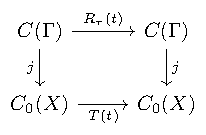
\includegraphics[width=0.35\textwidth]{./tikz-images/tikz-chap-b3.pdf}
\end{center}
%% --
Here, $(R_{\tau}(t))$ denotes the rotation semigroup%
\index{rotation semigroup} 
of period $\tau$ (see Part-I, Example~\ref{ex:a3-5.6}).
If\/ $X$ is compact, then $j$ is a topological embedding.
\end{corollary}
%% --
\begin{proof}
	Assume that $Ah = \im\alpha h$, $\alpha > 0$, and let $\tilde{h}(x) \coloneq h(x)/|h(x)|$.
	Then we define $j$ by
	%% --
	\begin{equation}\label{eq:b3-3.9}
	j(f) \coloneq |h|\cdot f\circ\tilde{h} \quad \left(\text{\ie\ }(j(f))(x) = |h(x)|\cdot f(\tilde{h}(x))\right).
	\end{equation}
	%% --
	Obviously, $j$ is a lattice homomorphism and because $h$ has no zeros and $\tilde{h}$ has a dense image in $\Gamma$ (Theorem~\ref{thm:b3-3.6}\,(iii)), it follows that $j$ is injective.
	For the functions $e_{n} \in C(\Gamma)$ given by $e_{n}(z) = z^{n}$ $(n \in \Z)$ one has $j(e_{n}) = h^{[n]}$ $(n \in \Z)$ and therefore by Theorem~\ref{thm:b3-2.4}
	%% --
    \[ 
    T(t)\circ j(e_{n}) = T(t)h^{[n]} = \eu^{\im n\alpha t}\cdot h^{[n]} 
    \]
    and
    \[
    j\circ R_{\tau}(t)(e_{n}) = j(\eu^{\im n\alpha t}e_{n}) = \eu^{\im n\alpha t}\cdot h^{[n]} .
    \]
    %% --
    Since $\{e_{n} \colon n \in \Z\}$ is a total subset of\/ $C(\Gamma)$, we have $T(t)\circ j = j\circ R_{\tau}(t)$ for every $t > 0$.
	
	If\/ $X$ is compact, then $\tilde{h}(X)$ is closed, hence $\tilde{h}$ is onto, moreover, $|h| \geq \epsilon$ for some $\epsilon > 0$, thus the definition of\/ $j$ implies that $\|j(f)\| \geq \epsilon\|f\|$ for every $f \in C(\Gamma)$.
\end{proof}
%% --
A consequence of Corollary~\ref{cor:b3-3.8} is the following. 
There exist positive functions $f_{1}$ and $f_{2}$ such that $T(t)f_{1}$ and $T(t)f_{2}$ have disjoint support for every $t \geq 0$ (consider the images under $j$ of two disjoint functions on $C(\Gamma)$).
This observation proves the following corollary.
%% --
\begin{corollary}\label{cor:b3-3.9}

	Suppose that the hypotheses of Theorem~\ref{thm:b3-3.6} are satisfied and that for some $t_{0} > 0$ we have $T(t_{0})f \gg 0$ whenever $f > 0$.
	Then $P\sigma(A)\cap \im\R = \{0\}$.
\end{corollary}
%% --
Corollary~\ref{cor:b3-3.9} can be applied if\/ $T(t_{0})$ is a kernel operator%
\index{operator!kernel} 
with strictly positive kernel.
We give some examples.
%% --
\begin{examples}\label{ex:b3-3.10}
%
	
	\begin{enumerate}[\upshape (i), wide, labelindent=.25em] 
	\item 
	We assume that the semigroup $(T(t))$ satisfies the hypotheses of Theorem~\ref{thm:b3-3.6} and that it is given by
	\[
	(T(t)f)(x) = \int_{X} k(t,x,y)f(y) \diff{\mu}(y) , 
	\]
	where $\mu$ is a positive measure and $k$ is a positive continuous function (see Example~\ref{ex:b3-3.4}\,(ii)).
	We will show that $P\sigma(A)\cap(s(A) + \im\R) = \{s(A)\}$.
	
	Assuming the contrary, by Theorem~\ref{thm:b3-3.6}\,(iv) there exist $\alpha \neq 0$, $h \in C_{0}(X)$ such that
	%% --	
	\begin{equation}\label{eq:b3-3.10}
	S_{h}^{-1}T(t)\circ S_{h} = \eu^{\im\alpha t}\cdot T(t) \text{ for all } t \geq 0.
	\end{equation}
	%% --
	This implies that $k$ satisfies
	%% --	
	\begin{equation}\label{eq:b3-3.11}
	\frac{\overline{h(x)}}{|h(x)|}\cdot\frac{h(y)}{|h(y)|}\cdot k(t,x,y) = \eu^{\im\alpha t}k(t,x,y) \quad (t > 0, x,y \in X).
	\end{equation}
	%% --
	It follows that for $0 < |s-t| < 2\pi/\alpha$ the kernel functions  $k(t,\cdot,\cdot)$ and $k(s,\cdot,\cdot)$ have disjoint support.
	This is impossible if\/ $k$ is continuous.
	
	\item 
	Let $\Omega$ be a domain in $\R^{n}$ and define $L_{0}$ as
	\[
	L_{0}f \coloneq \sum_{i,j=1}^{n} a_{ij}f_{ij}'' + \sum_{i=1}^{n}b_{i}f_{i}' + cf , 
	\]
	with domain 
    \[
    D(L_{0}) \coloneq \{f \in C_{0}(\Omega) \colon f \in  C^{\infty}, L_{0}f \in C_{0}(\Omega)\} , 
    \]
	where $f_{i}'$ stands for $\partial f/\partial x_{i}$, and $f_{ij}'' = \partial^{2}f/\partial x_{i}\partial x_{j}$.
	
	Suppose that $L_{0}$ is elliptic, $a_{ij}$, $b_{i}$, $c$ are real-valued $C^{\infty}$-functions and $\sup_x c(x) < \infty$, assume further that the closure $L$ of\/ $L_{0}$ is the generator of a positive semigroup on $C_{0}(\Omega)$ which has compact resolvent.
	For example, this is true if the boundary  $\partial\Omega$ is $C^{\infty}$ and $a_{ij} \in C^{\infty}(\overline{\Omega})$ (\cf Theorem~4.8.3 of \textcite{fattorini:1983}).
	We will show that 
    \[
    P\sigma(L)\cap(s(L) + \im\R) = \{s(L)\} .
    \]
	In order to apply Theorem~\ref{thm:b3-3.6}, we have to show that the corresponding semigroup $(T(t))$ is irreducible.
	Given $0 < f \in C_{0}(\Omega)$, then there is $g \in D(L_{0})$ such that $0 < g \leq f$. The function 
	$h \coloneq R(\lambda,L)g$ is $C^{\infty}$ (Weyl's Lemma) and satisfies 
    \[
    L_{0}h - \lambda h = -g < 0 .
    \]
	Assuming that $\lambda > \lambda_{0} \coloneq \sup_x c(x)$, then $h$ is positive, even strictly positive by the maximum principle \textcite[Chapter~2, Theorem~6]{protterweinberger:1967}.
	Thus we have  
    \[ 
    R(\lambda,L)f \geq R(\lambda,L)g = h \gg 0 \text{ for every } f>0 
    \]
    showing that $(T(t))$ is irreducible (see Definition~\ref{def:b3-3.1}\,(e)).

Next we apply Theorem~\ref{thm:b3-3.6}\,(iv) in order to show that the spectral bound is a dominant eigenvalue.
	We can assume that $s(L) = 0$.
	If\/ $s(L)$ is not dominant, then by Theorem~\ref{thm:b3-3.6}\,(iv) we have
	
	\begin{equation}\label{eq:b3-3.12}
		L_{0}h = \im\alpha h, \quad L_{0}|h| = 0, \quad L_0\bar{h} = -\im\alpha \bar{h} 
		\text{ for some } h \ne 0, \alpha > 0.
	\end{equation}
%% --
If we define $u \coloneq |h|$ and $w \coloneq h/|h|$, then Eq.~\myeqpageref{eq:b3-3.12} reads
	 \begin{equation}\label{eq:b3-3.13}
	L_{0}(uw) = \im\alpha uw, \quad L_{0}(u) = 0, \quad L_{0}(u/w) = -\im\alpha\cdot u/w .
	\end{equation}
	Explicit calculation of\/ $L_{0}(uw)$ and $L_{0}(u/w)$ using the product formula yields
		\begin{equation}\label{eq:b3-3.14}
		\begin{split}
		L_{0}(uw) &=  wL_{0}(u) + u\sum_{i,j} a_{ij}w_{ij}'' + \sum_{i}\left(ub_{i} + 2\sum_{j} a_{ij}u_{j}'\right)w_{i}',\\
		L_{0}(u/w) &= \frac{1}{w}L_{0}(u) + u\sum_{i,j}a_{ij}(1/w)_{ij}'' + \sum_{i}\left(ub_{i} + 2\sum_{j} a_{ij}u_{j}'\right)(1/w)_{i}'.
		\end{split}
	\end{equation}
%% --
	Observing that $(1/w)_{i}' = -w^{-2}\cdot w_{i}'$ and $(1/w)_{ij}'' = w^{-3}\cdot(2w_{i}'w_{j}' - ww_{ij}'')$, we obtain
%% --
		\begin{equation}\label{eq:b3-3.15}
			L_{0}(uw) + w^{2}L_{0}(u/w) = 2wL_{0}(u) + 2u/w\cdot\sum_{i,j} a_{ij}w_{i}'w_{j}'.
		\end{equation}
%% --
	This identity and Eq.~\myeqpageref{eq:b3-3.13} implies that $2u/w\cdot\sum_{i,j} a_{ij}w_{i}'w_{j}' = 0$.
	Since $|w| = 1$, we have $w_{i}' = \im\theta_{i}w$ with real-valued functions $\theta_{i}$, hence $\sum_{i,j} a_{ij}w_{i}'w_{j}' = -w^{2}\sum_{i,j} a_{ij}\theta_{i}\theta_{j}$. Since $u$ has no zeros and $(a_{ij})$ is positive definite, we obtain $\theta_{i} = 0$, \ie $\text{grad } w = (w_{i}') = 0$ in $\Omega$, hence $w = \text{const}$.
	Then, by Eq.~\myeqpageref{eq:b3-3.13}, we have $\im \alpha uw = L_{0}(uw) = wL_{0}(u) = 0$, a contradiction.

	The assumption that $L_{0}$ is elliptic, \ie that $(a_{ij})$ is positive definite, is essential in order to show that there is only one eigenvalue in the boundary spectrum.
	In the following example $(a_{ij})$ is positive semi-definite and $P\sigma_{b}(L) = s(L) + \im\alpha\Z$.
	
	\item 
	We consider 
    \[
    \Omega = \{(x,y) \in \R^{2} \colon 1 < (x^{2} + y^{2})^{1/2} < 2\} , 
    \]
    and the second order differential operator $L_{0}$ given by
    \index{differential operator}
    %%
	\[
	(L_{0}f)(x,y) = 1/(x^{2} + y^{2})\cdot(x^{2}f_{xx} + 2xyf_{xy} + y^{2}f_{yy}) + (xf_{y} - yf_{x}).
	\]
    %%
	The assertion concerning the boundary spectrum can be verified easily by using polar coordinates, $x = r\cdot\cos\omega$, $y = r\cdot\sin\omega$.
	Then $L_{0}$ becomes $L_{0}f = f_{rr} + f_{\omega}$ on the space $C_{0}(1,2) \otimes C_{2\pi}(\R)$.
	\end{enumerate}
\end{examples}
%% --
In this section we have seen that the eigenvalues in the boundary spectrum of an irreducible semigroup form a subgroup of\/ $\im \R$ (provided that $s(A) = 0$).
We conclude this section mentioning an analogous statement for the whole boundary spectrum of Markov semigroups on $C(K)$, $K$ compact.
It seems to be unknown if this is true for irreducible semigroups in general.
To prove this result one uses the proof of the analogous result for a single operator (\cf \textcite[Theorem~7]{schaefer:1968}) as a guideline.
%% --
\begin{theorem}\label{thm:b3-3.11}
%%
    \index{spectrum!irreducible semigroup}
	Suppose that $(T(t))$ is an irreducible semigroup of Markov operators%
    \index{operator!Markov} 
    on $C(K)$, $K$ compact.
	Then $\sigma_{b}(A)$ is a closed subgroup of\/ $\im \R$, \ie
   \[%\textstyle
   \text{either}\quad \sigma_{b}(A) = \{0\}\quad\text{or}\quad \sigma_{b}(A) = \im\R\quad\text{or}\quad\sigma_{b}(A) =\im\alpha\Z \text{  for some } \alpha > 0 .
   \]
\end{theorem}
\index{irreducible semigroup|)}
\index{semigroup!irreducible semigroup|)}
%% --
%% --
\section{Semigroups of Lattice Homomorphisms}\label{sec:b3-4}%
\index{lattice homomorphism|(}
\index{semigroup!lattice semigroup}
%% --
As we have seen in Section~\ref{sec:b3-2} the boundary spectrum of many positive semigroups is a cyclic set.
However, there are hardly any restrictions on the set 
%% --
\[
\{\lambda \in \sigma(A) \colon \Re(\lambda) < s(A)\} , 
\] 
%% --
except that it is symmetric with respect to the real axis.
For semigroups of lattice homomorphisms the situation is quite different.
We will show that the whole spectrum is an imaginary additively cyclic 
subset of\/ $\C$ (see Definition~\ref{def:b3-2.5}).
A complete proof of this result requires some facts of the theory of Banach lattices, therefore, we postpone it to Part-III, Theorem~\ref{thm:c3-4.2}.
%% --
\begin{theorem}\label{thm:b3-4.1}
\index{spectrum!cyclic}
%% --
If\/ $A$ is the generator of a semigroup of lattice homomorphisms, then $\sigma(A)$, $A\sigma(A)$ and $P\sigma(A)$ are cyclic subsets of\/ $\C$.
\end{theorem}
%% --
\begin{proof}[First part of the proof]
We prove the assertion concerning $A\sigma(A)$ and $P\sigma(A)$.
	Assume that 
    \[
    Ah = (\alpha + \im\beta)h, \quad \alpha,\beta \in \R, \quad h \neq 0 , 
    \]
    then by Part-I, Corollary~\ref{cor:a3-6.4}
    \[
    T(t)h = \eu^{\alpha t}\eu^{\im\beta  t}h \text{ for all } t \geq 0 .
    \]
	Since $T(t)$ is a lattice homomorphism we have 
    \[
    T(t)|h| = |T(t)h| = \eu^{\alpha t}|h|\, (t \geq 0)
    \quad\text{or}\quad A|h| = \alpha|h| , 
    \] 
    hence by Theorem~\ref{thm:b3-2.4}\,(ii)
    \[
    Ah^{[n]} = (\alpha + \im n\beta)h^{[n]} \text{ for all } n \in \Z .
    \]
	We have shown that $P\sigma(A)$ is cyclic.
	
	To prove that $A\sigma(A)$ is cyclic as well, one considers a semigroup $\mathcal{F}$-product $E_{\mathcal{F}}^{\TT}$ of\/ $E$ 
	(see Part-I, Section~\ref{subsec:a1-3.7}).
    \index{semigroup!F-product@$\mathcal{F}$-product}
	It is easy to see that $E_{\mathcal{F}}^{\TT}$ is a Banach lattice 
	and $(T_{\mathcal{F}}(t))$ is a semigroup of lattice homomorphisms.
	Part-I, Proposition~\ref{prop:a3-4.4} implies $A\sigma(A) = P\sigma(A_{\mathcal{F}})$.
	Thus the assertion follows from the cyclicity of point spectrum.
\end{proof}
%% --
\index{semiflow|(}
Performing a similar construction as in Example~\ref{ex:b3-2.6}\,(vi) one can show that every closed cyclic subset of\/ $\C$  which is contained in a left halfplane is the spectrum of a suitable semigroup of lattice homomorphisms. 
For details see \textcite{derndingernagel:1979}. 
In the following we restrict ourselves to the case of compact spaces. 
Then a semigroup of lattice homomorphisms can be described explicitly by a semiflow $\phi$, and real-valued functions $h$ and $p$ (see Theorem~\ref{thm:b2-3.5} and Theorem~\ref{thm:b2-3.6}). 
The function $p$ has no influence on spectral properties (\cf Eq.~\myeqpageref{eq:b2-3.7}). 
Therefore we will assume that $(T(t))$ has the following form (\cf Theorem~\ref{thm:b2-3.5}). 
%% --
\begin{equation}\label{eq:b3-4.1}
	T(t)f = h_{t}\cdot f\circ\phi_{t} \quad (t \geq 0, f \in C(K)) 
\end{equation}
%% --
where 
\[
\phi = (\phi_{t}) \colon \R_{+} \times K \to K , \ \phi_{t+s}
=\phi_{t}\circ\phi_{s}  
\ (t,\,s \geq 0) , 
\]
is a continuous semiflow and 
\[
h_{t}(x) \coloneq \exp\left(\int_{0}^{t} h(\phi(s,x)) \ds\right)\ (t \geq 0,\, x \in K)
\]
are multipliers for some continuous function $h \colon K \to \R$.
In the following we will describe the spectrum of the semigroup given by Eq.~\myeqpageref{eq:b3-4.1} in terms of\/ $\phi$ and $h$.

At first we have to fix some notation.
Let $K$, $\phi$, $h$ be as in Eq.~\myeqpageref{eq:b3-4.1}. 
Define
%% --
\begin{equation}\label{eq:b3-4.2}
K_{t} \coloneq \phi_{t}(K) \quad \text{for } t < \infty,\quad\text{and}\quad K_{\infty} \coloneq \bigcap_{t < \infty} K_{t}.
\end{equation}
%% --
Some properties of the sets $K_t$  are listed in the following lemma.
The proof is not difficult and will be omitted. 
%% --
\begin{lemma}\label{lem:b3-4.2}%
\index{semiflow}
%% --
Every $K_{t}$ $(0 \leq t \leq \infty)$ is a non-empty closed subset of\/ $K$ which is invariant under the semiflow $\phi$.
	Moreover, the following assertions are true.
	\begin{enumerate}[\upshape (i)]
		\item 
		For $s > t$ we have $K_{s} \subseteq K_{t}$.
		In case that $K_{s} = K_{t}$ then $K_{t} = K_{\infty}$.
		
		\item
		$\phi_{t}(K_{\infty}) = K_{\infty}$ for all $t \geq 0$.
		
		\item 
		If one partial mapping $\phi_{t}$, $t > 0$, is injective (surjective), then all mappings $\phi_{s}$ are injective (surjective).
	\end{enumerate}
\end{lemma}
%% --
We call a \emph{semiflow} $\phi$ \emph{injective (surjective)} if one and hence all of the partial mappings $\phi_{t}$ are injective (surjective).
Studying the spectrum of the semigroup given by Eq.~\myeqpageref{eq:b3-4.1} we divide the complex plane into these three sets
%% --
\begin{equation}\label{eq:b3-4.3}
	\begin{split}	 
		&\{\lambda \in \C \colon \Re(\lambda) < \underline{c}(h,\phi)\} ,  \\
		&\{\lambda \in \C \colon \underline{c}(h,\phi) \leq \Re(\lambda) \leq \overline{c}(h,\phi)\} ,  \\
		&\{\lambda \in \C \colon \overline{c}(h,\phi) < \Re(\lambda)\}.
	\end{split}
\end{equation}
%% --
The quantities $\underline{c}(h,\phi)$ and $\overline{c}(h,\phi)$ are defined as follows.
\begin{align}\label{eq:b3-4.4}\notag
		\overline{c}(h,\phi) &\coloneq \lim_{t\to\infty} \overline{c}_{t}(h,\phi) = \inf_{t>0} \overline{c}_{t}(h,\phi) ,  \\ \notag
        &\text{ where }
		\overline{c}_{t}(h,\phi) \coloneq \sup_{x\in K} \mleft\{\frac{1}{t}\int_{0}^{t} h(\phi(s,x)) \ds \mright\} , \notag
        \\& \\ \notag
		\underline{c}(h,\phi) &\coloneq \lim_{t\to\infty} \underline{c}_{t}(h,\phi) = \sup_{t>0} \underline{c}_{t}(h,\phi) ,  \\ \notag
        &\text{ where } 
		\underline{c}_{t}(h,\phi) \coloneq \inf_{x\in K} \mleft\{\frac{1}{t}\int_{0}^{t} h(\phi(s,x)) \ds\mright\} .
\end{align}
%% --
It is easy to see that $\overline{c}_{t}(h,\phi) = 1/t\cdot\log\|T(t)\|$, hence in the definition of\/ $\overline{c}(h,\phi)$, both the limit and the infimum exist and coincide with the growth bound (see Part-I, Eq.~\myeqpageref{eq:a1-1.1}).
Furthermore, $\underline{c}_{t}(h,\phi) = -\overline{c}_{t}(-h,\phi)$.
Therefore, $\underline{c}(h,\phi)$ is well defined too.

First we will describe the part of\/ $\sigma(A)$ which is contained in the left half-plane determined by $\underline{c}(h,\phi)$.
It turns out that either the whole half-plane is contained in $\sigma(A)$ or it has empty intersection with $\sigma(A)$.
This depends only on properties of\/ $\phi$.
Essentially there 
are three different cases. 
Before we state the general result (see Theorem~\ref{thm:b3-4.4}) we give some typical examples.
%% 
\begin{examples}\label{ex:b3-4.3}
	\begin{enumerate}[\upshape (i), wide, labelindent=.25em]
	\item 
	Consider on $K = [0,\infty]$ the semiflow defined by 
    \[
    \phi(t,x) \coloneq x + t,\ (\infty + t = \infty) .
    \]
	Then $K_{t} = [t,\infty]$ and $K_{\infty} = \{\infty\}$.
	The spectrum of the corresponding semigroup $T(t)f = f\circ\phi_{t}$ is 
    \[
    \sigma(A) = A\sigma(A) = 
    \{\lambda \in \C \colon \Re(\lambda) \leq 0\} .
    \]
	
	\item 
	Consider again $K = [0,\infty]$ and define a semiflow by
	\[
	\phi(t,x) \coloneq \begin{cases} 
		x - t & \text{if } x \geq t  , \\
		0 & \text{if } x < t .
	\end{cases} \quad (\infty - t = \infty) .
	\]
	Then $K_{t} = K$ for all $t$, hence $K_{\infty} = K$ and \[
    \sigma(A) = \{\lambda \in \C \colon \Re(\lambda) \leq 0\} ,  \ R\sigma(A) = \{\lambda \in \C \colon \Re(\lambda) < 0\} \cup \{0\} .
    \]
	
	\item 
	Consider on $K_{1} \coloneq [-1,\infty)$ the equivalence relation defined by
\enquote{$x \sim y$} if and only if
%% --
\[
    x,\,y \geq 0 \quad\text{and}\quad x - y \in \Z.
\]
%% --
The semiflow $\phi_{1}$ on $K_{1}$ given by $\phi_{1}(t,x) = x + t$
induces a semiflow $\phi$ on $K \coloneq K_{1}/{\sim}$.
    
	For $0 < t < 1$ we have $K \neq K_{t} \neq K_{\infty}$ $(K_{\infty} = [0,1]/{\sim} \cong \Gamma)$.
	The spectrum is $\sigma(A) = 2\pi \im\Z$.
%%KKG 2025-12-19
    \index{semiflow|)}
	
	\item 
	Consider on $K = [-1,1]$ the flow $\phi$ given by
	\[
	\phi(t,x)\coloneq \begin{cases}
		-1 & \text{if } x < 0 \text{ and } t > -\frac{x+1}{x}  ,  \\
		\frac{x}{1+tx} & \text{otherwise.}
	\end{cases}
	\]
	Then $K_{t} = [-1,\frac{1}{1+t}]$, $K_{\infty} = [-1,0]$ and
	\[
	\sigma(A) = \{\lambda \in \C \colon \Re(\lambda) \leq 0\},\quad 
	\{\lambda \in \C \colon \Re(\lambda) < 0\} \subsetneq A\sigma(A)\cap R\sigma(A).
	\]
	\end{enumerate}
\end{examples}
%% --
\begin{theorem}\label{thm:b3-4.4}
	Suppose $\TT$ is a semigroup of lattice homomorphisms given by Eq.~\myeqpageref{eq:b3-4.1} with generator $A$.
	Considering $H \coloneq \{\lambda \in \C \colon \Re(\lambda) < \underline{c}(h,\phi)\}$, where $\underline{c}(h,\phi)$ is given by Eq.~\myeqpageref{eq:b3-4.4}, then we have:
	\begin{enumerate}[\upshape (i)]
		\item 
		If\/ $K_{t} \neq K_{\infty}$ for every $t < \infty$, then $H \subseteq A\sigma(A)$.
	
		\item 
		If\/ $\phi_{|K_{\infty}}$ is not injective, then $H \subseteq R\sigma(A)$.
	
		\item 
		If\/ $K_{s} = K_{\infty}$ for some $s < \infty$ and $\phi_{|K_{\infty}}$ is injective, then $H\cap\sigma(A) = \emptyset$.
	\end{enumerate} 
\end{theorem}
%% --
\begin{proof}
	For $\epsilon > 0$ we define $H_{\epsilon} = \{\lambda \in \C \colon \Re(\lambda) < \underline{c}(h,\phi)-\epsilon\}$.
	Obviously it is enough to prove assertions (i), (ii) and (iii) respectively for $H_{2\epsilon}$, $\epsilon> 0$ arbitrary, instead of\/ $H$.

	(i) By the definition given in Eq.~\myeqpageref{eq:b3-4.4} there exists a $\tau > 0$ such that $\underline{c}_{t}(h,\phi) \geq \underline{c}(h,\phi) - \epsilon$ for all $t \geq \tau$.
	It follows that
	%% --
	\begin{equation}\label{eq:b3-4.5}
		h_{t}(x) \geq \eu^{(\alpha + \epsilon)t} \text{ whenever } t \geq \tau, x \in K, \alpha < \underline{c}(h,\phi)-2\epsilon .
	\end{equation}
	%% --
	Now we fix $\lambda = a + \im\beta \in H_{2\epsilon}$ $(a,\beta \in \R)$ and construct an approximate eigenvector $(g_{n})$ of\/ $A$ 
    \index{approximate eigenvector} 
    corresponding to $\lambda$.
	For $n \leq \tau + 1$ we choose an arbitrary function $g_{n} \neq 0$.
	Now suppose $n > \tau + 1$.
	We choose $x_{n} \in K_{n+1/2} \setminus K_{n+1}$ (\cf Lemma~\ref{lem:b3-4.2}\,(i)), then there exists $y_{n} \in K$ such that $\phi(n+1/2,y_{n}) = x_{n}$.
	We have $\phi([0,n+1/2],y_{n}) \cap K_{n+1} = \emptyset$ and the mapping $t \mapsto \phi(t,y_{n})$ is a continuous injection, hence a homeomorphism from $[0,n+1/2]$ into $K$ (this is true because $\phi(n+1/2,y_{n}) \notin K_{n+1}$).
	By Tietze's Theorem there is $f_{n} \in C(K)$ such that
	%% --
	\begin{equation}\label{eq:b3-4.6}
		\begin{aligned}
			\|f_{n}\| \leq 1 &, \quad {f_{n}|}_{K_{n+1}} = 0 ,  \\
			f_{n}(\phi(t,y_{n})) &= 0 \text{ for } 0 \leq t \leq n-(1+\delta) \text{ and } n+\delta \leq t \leq n+1 ,  \\
			f_{n}(\phi(t,y_{n})) &= \eu^{\im\beta  t} \text{ for } n-1 \leq t \leq n .
		\end{aligned}
	\end{equation}
	%% --
	The constant $\delta \in (0,1/2)$ will be determined later.
	
	Considering $g_{n}\coloneq \int_{0}^{n+1} \eu^{-\lambda t} T(t)f_{n} \dt$, then $g_{n} \in D(A)$ and
	%% --
	\begin{equation}\label{eq:b3-4.7}
		(\lambda - A)g_{n} = (\Id - \eu^{-\lambda(n+1)}T(n+1))f_{n} = f_{n} - \eu^{-\lambda(n+1)} \cdot h_{n+1} \cdot f_{n} \circ \phi_{n+1} = f_{n}.
	\end{equation}
	%% --
	Moreover,
	%% --
	\begin{multline*}
	\|g_{n}\| \geq |g_{n}(y_{n})| = \left|\int_{0}^{n+1} \eu^{-\lambda t} h_{t}(y_{n})f_{n}(\phi(t,y_{n})) \dt \right| \\
	\geq \left|\int_{n-1}^{n} \eu^{-\lambda t} h_{t}(y_{n}) \eu^{\im\beta  t} \dt\right| - \left[\int_{n-(1+\delta)}^{n-1} + \int_{n}^{n+\delta}\left| \eu^{-\lambda t}h_{t}(y_{n})f_{n}(\phi(t,y_{n}))\right| \dt\right] \\
	\geq \int_{n-1}^{n} \eu^{-at} \eu^{(a+\epsilon)t} \dt - \left[\int_{n-(1+\delta)}^{n-1} + \int_{n}^{n+\delta} \eu^{-at}|h_{t}(y_{n})| \dt\right] \\
	= \frac{1}{\epsilon}\cdot\left(\eu^{\epsilon n} - \eu^{\epsilon(n-1)}\right) - \mleft(\int_{n-(1+\delta)}^{n-1} + \int_{n}^{n+\delta} \eu^{-at}|h_{t}(y_{n})| \dt\mright) .
	\end{multline*}
	The constant $\delta$ can be chosen such that
	%% --
	\begin{equation}\label{eq:b3-4.8}
		\|g_{n}\| \geq 1/(2\epsilon)\cdot\left(\eu^{\epsilon n} - \eu^{\epsilon(n-1)}\right) \to \infty \text{ for } n \to \infty.
	\end{equation}
	%% --
	It follows from Eq.~\myeqpageref{eq:b3-4.8} and Eq.~\myeqpageref{eq:b3-4.7} that $ g_n / \|g_n\|$ is an approximate
	eigenvector of\/ $A$ corresponding to $\lambda$. 
    Thus (i) is proved. 
	
	The 
	proofs of (ii) and (iii) will be handled simultaneously. 
    First we show that we can restrict attention to the case where $K = K_\infty$.
	
	Indeed, $K_{\infty}$ is a $\phi$-invariant subset, hence \[
    I_{\infty}\coloneq \{f \in C(K) \colon f|_{K_{\infty}} = 0\}
    \]
    %% --
    is a $\TT$-invariant ideal.
	Identifying $C(K)/I_{\infty}$ with $C(K_{\infty})$ (\cf Section~\ref{sec:b1-1}), then $(T_{/I_{\infty}}(t))$ is the semigroup governed by $\phi_{|K_{\infty}}$ and $h_{|K_{\infty}}$.
    
	Since one always has $R\sigma(A_{/I_{\infty}}) \subseteq R{\sigma}(A)$, assertion (ii) is proved, 
	when we can show that $H_{2\epsilon} \subseteq R\sigma(A_{/I_{\infty}})$.
    
	In case (iii) one has $K_{s} = K_{\infty}$ for some $s < \infty$, which implies $T(s)_{|I_{\infty}} = 0$.
	Hence we have $\sigma(A_{|I_{\infty}}) = \emptyset$ and therefore $\sigma(A) = \sigma(A_{/I_{\infty}})$ by Part-I, Proposition~\ref{prop:a3-4.2}.
	
	Henceforth we will assume that $K = K_{\infty}$, that is, $\phi$ is surjective (\cf Lemma~\ref{lem:b3-4.2}\,(ii)).
	
	We choose $\tau > 0$ such that Eq.~\myeqpageref{eq:b3-4.5} is true.
	Since $\phi$ is surjective, for every $f \in C(K)$ there is an $x_{f} \in K$ such that $\|f\| = |f(\phi(\tau,x_{f}))|$ and we obtain for $\lambda \in H_{2\epsilon}$, $\lambda = a + \im\beta$, $a,\beta \in \R$
	%% --
	\begin{equation}\label{eq:b3-4.9}
		\begin{aligned}
			\|(\eu^{\lambda\tau} - T(\tau))f\| &\geq |h_{\tau}(x_{f})f(\phi(\tau,x_{f})) - \eu^{\lambda\tau}f(x_{f})| \\
			& \geq h_{\tau}(x_{f})\|f\| - \eu^{a\tau}|f(x_{f})| 
			 \geq \eu^{(a+\epsilon)\tau}\|f\| - \eu^{a\tau}\|f\| \\
			&= \eu^{a\tau}(\eu^{\epsilon\tau} - 1)\|f\|.
		\end{aligned}
	\end{equation}
	%% --
	It follows that the disc 
    \[
    D \coloneq \{\lambda \in \C \colon |\lambda| < \exp((\underline{c}(h,\phi)-2\epsilon)\tau)\}
    \]
    has an empty intersection with $A{\sigma}(T(\tau))$ and therefore $H_{2\epsilon}\cap A\sigma(A) = \emptyset$ by Part-I, Proposition~\ref{prop:a3-6.2}.
	Since every boundary point of the spectrum is an approximate eigenvalue (by Part-I, Proposition~\ref{prop:a3-2.2}\,(i)) we have the following alternative.
	%% --
	\begin{equation}\label{eq:b3-4.10}
		\begin{aligned}
		&\text{Either } D \subseteq \rho(T(\tau)) \text{ and } H_{2\epsilon} \subseteq \rho(A) \\
		&\text{ or } D \subseteq R{\sigma}(T(\tau)) \text{ and } H_{2\epsilon} \subseteq R{\sigma}(A).
	\end{aligned}
	\end{equation}
	%% --
	It is not difficult to see that $0 \in \rho(T(\tau))$ whenever $\phi_{t}$ is bijective and that $0$ is an eigenvalue of\/ $T(\tau)'$ if\/ $\phi_{\tau}$ is not injective.
	Since we assumed that $\phi$ is surjective, assertions (ii) and (iii) of the theorem are immediate consequences of Eq.~\myeqpageref{eq:b3-4.10}.
\end{proof}
%% --
The Examples~\ref{ex:b3-4.3}\,(i), (ii) and (iii) respectively are prototypes of the three different cases considered in Theorem~\ref{thm:b3-4.4}.
Example~\ref{ex:b3-4.3}\,(iii) also shows that there are semigroups whose spectrum is contained in a right half-plane, although they cannot be embedded in a group (compare Corollary~\ref{cor:b3-4.5} below).
Example~\ref{ex:b3-4.3}\,(iv) shows that (i) and (ii) do not exclude each other.
%% --
\begin{corollary}\label{cor:b3-4.5}
	If\/ $\phi$ is injective or surjective, then the following assertions are equivalent.
	\begin{enumerate}[\upshape (a)]
		\item 
		$A$ is the generator of a strongly continuous group.
		
		\item 
		$\sigma(A)$ is contained in a right half-plane.
	\end{enumerate}
\end{corollary}
%% --
\begin{proof}
	(a)~$\implies$~(b):\ \  holds true because $-A$ is a generator of a semigroup.
	
	(b)~$\implies$~(a):\ \ 
	We have to show that one (hence each) operator $T(t)$, $t > 0$ is invertible.
	Obviously this is true if\/ $\phi$ is bijective.
	At first we assume that $\phi$ is surjective, that is, $K = K_{\infty}$.
	By Theorem~\ref{thm:b3-4.4} we have that $\phi_{|K_{\infty}}$ is injective if (b) is true.
	Thus $\phi$ is bijective.
	Now we assume that $\phi$ is injective.
	We have to show that $K = K_{\infty}$.
	By Theorem~\ref{thm:b3-4.4} we have $K_{\infty} = K_{s}$ for some $s$, whenever (b) is true.
	Given $x \in K$ then by Lemma~\ref{lem:b3-4.2}\,(ii) there exists $y \in K_{\infty}$ such that $\phi(s,x) = \phi(s,y)$.
	If\/ $\phi$ is injective we have $x = y \in K_{\infty}$.
\end{proof}
%% --
\begin{example}\label{ex:b3-4.6}
	Suppose $F \colon \R^n \to \R^n$ is continuously differentiable.
	We denote the maximal flow corresponding to the differential equation%
    \index{differential equation} 
    $y' = F(y)$ by $\phi_{0}$.
	In general, $\phi_{0}$ is only defined on an open subset of\/ $\R \times \R^n$ which contains $\{0\} \times \R^n$.
	For $x \in \R^n$ there exist $\underline{t}_{x}$ and $\overline{t}_{x}$ such that
	%% --
	\begin{equation}\label{eq:b3-4.11}
		\begin{aligned}
			&-\infty \leq \underline{t}_{x} < 0 < \overline{t}_{x} \leq \infty ,  \\
			&\phi_{0}(t,x) \text{ is defined if } \underline{t}_{x} < t < \overline{t}_{x} ,  \\
			&\text{if } \overline{t}_{x} < \infty \text{ (}\underline{t}_{x} > -\infty\text{)} \text{ then } |\phi_{0}(t,x)| \to \infty \text{ as } t\uparrow\overline{t}_{x} \text{ (}t\downarrow\underline{t}_{x}\text{)}.
		\end{aligned}
	\end{equation}
	%% --
	For details see Section~18.2 of \textcite{dieudonne:1971}.
	\begin{enumerate}[\upshape (i), wide, labelindent=.25em]
	\item
	If\/ $\phi_{0}$ is a global flow, \ie if\/ $\phi_{0}$ is defined on $\R \times \R^n$, then one has a corresponding (semi-)group on $C_{0}(\R^n)$.
	If\/ $F$ is differentiable, its generator is the closure of\/ $A_{1}$ which is defined as follows (\cf Example~\ref{ex:b2-3.15}).
	%% --
	\begin{equation}\label{eq:b3-4.12}
		\begin{aligned}
			A_{1}f = (F|\text{grad }f) \coloneq 
            {  \sum_i F_{i} \cdot \partial_{i}f}  ,  \\
			D(A_{1}) \coloneq \{f \in C^1 \colon \supp(f)  \text{ is compact}\}.
		\end{aligned}
	\end{equation}
	%% --
	Then $\phi_{0}$ can be uniquely extended to a flow $\tilde{\phi}_{0}$ on $\R^n\cup\{\infty\}$ by defining $\tilde{\phi}_{0}(t,\infty) \coloneq \infty$ for all $t \in \R$.
	$\phi_{0}$ and $\tilde{\phi}_{0}$ satisfy condition (iii) of Theorem~\ref{thm:b3-4.4}.

%%KKG 2025-12-19
    \index{semiflow|(}
    A global flow exists if\/ $F$ is globally Lipschitz continuous or uniformly bounded. 
    For $\{x \in \R^n \colon (x|F(x)) > 0\}$ bounded in $\R^n$, a global semiflow always exists (\cf \textcite[Section~5.2]{deimling:1977}).
    
	\item 
	Now we do not assume that  $\phi_0$ is globally defined.
	Instead we consider a bounded domain $\Omega \subseteq \R^n$ with smooth boundary $\partial\Omega$ such that $(F(x)|\nu(x)) > 0$ for every $x \in \partial\Omega$, where $\nu(x)$ denotes the outward normal vector.
	
	Then for $x \in \overline{\Omega}$ we have $\underline{t}_{x} = -\infty$.
	Moreover, either $\phi_{0}(t,x) \in \Omega$ for all $t \geq 0$ or else there exists a unique $s_{x}$ with $0 \leq s_{x} < \overline{t}_{x}$ such that $\phi_{0}(s_{x},x) \in \partial\Omega$.
	In the first case we write $s_{x} \coloneq \infty$.
	Then we define $\phi \colon \R_{+} \times \overline{\Omega} \to \overline{\Omega}$ as 
	%% --
	\[\phi(t,x) \coloneq \begin{cases}
		\phi_{0}(t,x) & \text{if } 0 \leq t < s_{x}  ,  \\
		\phi_{0}(s_{x},x) & \text{if } t \geq s_{x} .
	\end{cases} .\]
	%% --
	Then $\phi$ is a continuous semiflow on the compact set $K \coloneq \overline{\Omega}$.
	We have $K_{\infty} = K$ and $\phi_{|K_{\infty}}$ is not injective.
	
	In case $F$ is differentiable, the generator of the corresponding semigroup is the closure of the operator $A_{2}$ defined by
	%% --
	\[
	A_{2}f \coloneq (F|\text{grad }f), \quad D(A_{2}) \coloneq \{f \in C^1(\overline{\Omega}) \colon (F|\text{grad }f) = 0 \text{ on } \partial\Omega\}.	
	\]
	
	\item 
	We consider $\Omega$ as in (ii) and assume that $(F(x)|\nu(x)) \leq 0$ for every $x \in \partial\Omega$.
	Then for every $x \in \overline{\Omega}$ we have $\overline{t}_{x} = \infty$.
	Thus $\phi \coloneq {\phi_{0}}_{|\R_{+}\times\overline{\Omega}}$ is a continuous semiflow on $K \coloneq \overline{\Omega}$.
	
	If\/ $(F(x)|\nu(x)) < 0$ for some $x \in \partial\Omega$, we have $K_{t} \subsetneq K_{s}$ whenever $t > s$ and $\phi_{\vert K_{\infty}}$ is injective.
	For a differentiable vector field $F$, the generator of the corresponding semigroup is the closure of\/ $A_{3}$ defined as
	%% --
	\[
	A_{3}f \coloneq (F|\text{grad }f), \quad D(A_{3}) \coloneq C^1(\overline{\Omega}).
	\]
	%% --
\end{enumerate}
\end{example}
%% --
We conclude the discussion of semiflows associated with ordinary differential equations by remarking that the ideas of (ii) and (iii) can be combined to obtain semigroups for more general subsets $\Omega$.

We continue the discussion of the spectrum of semigroups of lattice homomorphisms on $C(K)$ given by Eq.~\myeqpageref{eq:b3-4.1}.
Theorem~\ref{thm:b3-4.4} gives a good description of the part contained in 
\[
\{\lambda \in \C \colon \Re(\lambda) < \underline{c}(h,\phi)\} .
\]
The half-plane 
\[
\{\lambda \in \C \colon \Re(\lambda) > \overline{c}(h,\phi)\}
\] 
is always a subset of the resolvent set (see Proposition~\ref{prop:b3-4.8}\,(i) below).
The description of the remaining part 
\[\{\lambda \in \sigma(A) \colon \underline{c}(h,\phi) \leq \Re(\lambda) \leq \overline{c}(h,\phi)\}
\]
is more difficult.
First we discuss some examples and then give a partial answer to this problem (see Proposition~\ref{prop:b3-4.8}\,(ii)--(v)).
%% --
\begin{example}\label{ex:b3-4.7}
	\begin{enumerate}[\upshape (i), wide, labelindent=.25em]
		\item 
		Consider the flow on $[-\frac{\pi}{2},\frac{\pi}{2}]$ defined by
		\[
		\phi(t,x)\coloneq \arctan(\tan x - t), \quad x \in [-{\pi}/{2},{\pi}/{2}], 
		t \in \R\
		\] 
		and a continuous function $h \colon [-\frac{\pi}{2},\frac{\pi}{2}] \to \R$ with $h(-\frac{\pi}{2}) \leq h(\frac{\pi}{2})$. The flow belongs to the differential equation $y' = -\cos^2y$. 
		Then we have $\underline{c}(h,\phi) = h(-\frac{\pi}{2})$ and $\overline{c}(h,\phi) = h(\frac{\pi}{2})$.
		The spectrum of the corresponding semigroup is given by 
		%% --
		\[
		\sigma(A) = \left\{\lambda \in \C \colon h(-\pi/2) \leq \Re(\lambda) \leq h(\pi/2)\right\}.
		\]
		%% --
		
		\item 
		Consider 
        \[
        K = \{z \in \C \colon 1 \leq |z| \leq 2\} = \{r\cdot \eu^{\im\omega} \colon \omega\in \R, 1 \leq r \leq 2\}
         \]
         and a continuous function $\kappa \colon [1,2] \to \R_+$.
		
		Let $\tilde{\phi}$ be the flow on $K$ governed by the differential equation $\dot{\omega} = \kappa(r)$, $\dot{r} = 0$, hence $\tilde{\phi}(t,r\cdot \eu^{\im\omega}) = r\cdot \eu^{\im(\omega + \kappa(r)t)}$.
		
		For a continuous function $h \colon K \to \R$ let $\hat{h}(r) \coloneq \frac{1}{2\pi}\int_{0}^{2\pi} h(r\cdot \eu^{\im t}) \dt$ $(1 \leq r \leq 2)$.
		The spectrum of the semigroup corresponding to $\tilde{\phi}$ and $h$ (\cf Eq.~\myeqpageref{eq:b3-4.1}) is given by
		%% --
		\[
		\sigma(A) = \overline{\{\hat{h}(r) +  \im k\kappa(r) \colon k \in \Z, 1 \leq r \leq 2\}} \cup \{h(z) \colon \kappa(|z|) = 0\}.
		\]
	\end{enumerate}
\end{example}
%% --
\begin{proposition}\label{prop:b3-4.8}
Suppose the semigroup $(T(t))_{t\geq 0}$ on $C(K)$ is given by 
Eq.~\myeqpageref{eq:b3-4.1} and let $\underline{c}(h,\phi)$, $\overline{c}(h,\phi)$ be defined as in Eq.~\myeqpageref{eq:b3-4.4}.
Then the following assertions hold.
%% --
\begin{enumerate}[\upshape (i)]
\item 
	$\{\lambda \in \C \colon \Re(\lambda) > \overline{c}(h,\phi)\} \subseteq \rho(A)$, 
		
\item 
	$\overline{c}(h,\phi)$ and $\underline{c}(h,\phi)$ are spectral values, 
		
\item 
	If\/ $\phi(t,x_{0}) = x_{0}$ for every $t \geq 0$, then $h(x_{0}) \in R{\sigma}(A)$, 
		
\item 
Assume $x_{0}$ has a finite orbit, \ie $\phi(\R_{+},x_{0}) = \phi([0,T],x_{0})$ for some $T < \infty$ and 
%% --
\[
\tau \coloneq \inf\{t > 0 \colon \phi(T+t,x_{0}) = \phi(T,x_{0})\} > 0, 
\]
%% --
then 
\[
\hat{h}(x_{0}) + \frac{2\pi}{\tau}\im\Z \subseteq R{\sigma}(A)\quad\text{where}\quad \hat{h}(x_{0}) \coloneq \frac{1}{\tau}\int_{T}^{T+\tau}h(\phi(s,x_{0}))\ds,
\]
		
\item 
	If\/ $x_{0}$ has an infinite orbit and 
	$\hat{h} \coloneq  \lim_{t\to\infty}h(\phi(t,x_{0}))$ exists, then 
    \[
    \hat{h} + \im\R \subseteq \sigma(A) .
    \]
\end{enumerate}
\end{proposition}
%% --
\begin{proof}	
	(i) and (ii): By Eq.~\myeqpageref{eq:b3-4.4} we have $\overline{c}_{t}(h,\phi) = 1/t\cdot\log\|T(t)\|$ hence $\overline{c}(h,\phi) = \omega_{0}(A)$ (\cf Eq.~\myeqpageref{eq:a1-1.1}).  
	Consequently, we have $\{\lambda \in \C \colon \Re(\lambda) > \overline{c}(h,\phi)\} \subseteq \rho(A)$ and $\overline{c}(h,\phi) \in \sigma(A)$ by Theorem~\ref{thm:b3-1.6}.
	
	To prove $\underline{c}(h,\phi) \in \sigma(A)$, we can assume by Theorem~\ref{thm:b3-4.4} that $K_{\infty} = K_{s}$ for some $s$ and that $\phi_{|K_{\infty}}$ is injective.
	It is easy to see that $\underline{c}(h,\phi) = \underline{c}(h_{|K_{\infty}},\phi_{|K_{\infty}})$, moreover, we have $\sigma(A_{|I_{\infty}}) = \emptyset$ hence $\sigma(A) = \sigma(A_{/I_{\infty}})$ by Part-I, Proposition~\ref{prop:a3-4.2}.
	This shows that we also can assume that $K = K_{\infty}$, \ie $\phi$ is bijective or $A$ is the generator of a group.
	Now the assertion follows from 
    \[
    \underline{c}(h,\phi) = \underline{c}(h,\phi^{-1}) = -\overline{c}(-h,\phi^{-1}) = -s(-A) .
    \]
	
	(iii) and (iv): One can check easily that in case of (iii) the Dirac functional $\delta_{x_{0}}$ is an eigenvector of\/ $A'$ corresponding to $h(x_{0})$.
    A little bit more calculation is necessary to check that in case of (iv) the functional $\phi_{k}$ defined by
%% --
\[
	\phi_{k}(f) \coloneq \int_{T}^{T+\tau} \exp\left(-\left(\hat{h}(x_{0}) + \im\cdot\frac{2\pi k}{\tau}\right) t\right)\cdot h_{t}(x_{0})\cdot f(\phi(t,x_{0})) \dt  \ (k \in \Z, f \in C(K))
\]
%% --
    is an eigenvector of\/ $A'$ corresponding to $\hat{h}(x_{0}) + \im\cdot\frac{2\pi k}{\tau}$.

    (v) Given $\beta \in \R$ we will show that $\hat{h} + \im\beta \in A\sigma(A') \subseteq \sigma(A)$.
    For $n,m \in \N$ we define a linear functional $\phi_{nm}$ as 
%% --
\[  
	\phi_{nm}(f) \coloneq \frac{1}{n}\int_{0}^{n} \exp(-(\hat{h}+\im\beta )t)\cdot h_{t}(\phi(m,x_{0}))\cdot f(\phi(m+t,x_{0})) \dt, \ f\in C(K).
\]
For $f \in D(A)$ we have 
%% --
	\begin{align*}
	&\left\langle(\hat{h}+\im\beta -A)f,\phi_{nm}\right\rangle = \\
	&  \frac{1}{n}\cdot\left(f(\phi(m,x_{0})) - \eu^{-\im\beta  n}\cdot % \exp(-\im\beta  n)
	\exp\left(\int_{m}^{m+n} (h(\phi(s,x_{0}))-\hat{h})\ds \right)f(\phi(m+n,x_{0}))\right).
	\end{align*}
%% --
It follows that $\phi_{nm} \in D(A')$ and, since $\lim_{t\to\infty} h(\phi(t,x_{0})) = \hat{h}$,
%% --
\begin{equation}\label{eq:b3-4.13}
	\limsup_{m\to\infty} \|(\hat{h}+\im\beta -A')\phi_{nm}\| \leq 2/n \text{ for every } n \in \N.
\end{equation}
%% --
Because the orbit is infinite we have
%% --
	\begin{align*}
	\|\phi_{nm}\| &= \frac{1}{n}\int_{0}^{n} \left|\eu^{-(\hat{h}+\im\beta )t} h_{t}(\phi(m,x_{0}))\right| \dt \\
	&= \frac{1}{n}\int_{0}^{n} \exp\left(\int_{m}^{m+t} (h(\phi(s,x_{0}))-\hat{h})\ds \right)\dt
	\end{align*}
%% --
which shows that
%% --
\begin{equation}\label{eq:b3-4.14}
	\lim_{m\to\infty} \|\phi_{nm}\| = 1 \text{ for every } n \in \N.
\end{equation}
%% --
In view of Eq.~\myeqpageref{eq:b3-4.13} and Eq.~\myeqpageref{eq:b3-4.14} it is not difficult to find a subsequence $k(n)$ of\/ $\N$ such that $(\phi_{n,k(n)})$ is an approximate eigenvector of\/ $A'$ corresponding to $\hat{h} + \im\beta$.
\end{proof}
%% --
We are now going to apply the results obtained so far to the special case where $h = 0$, \ie we consider semigroups of lattice homomorphisms which are Markov operators\index{operator!Markov}.
%% --
\begin{theorem}\label{thm:b3-4.9}
	Suppose $\TT$ is a semigroup of Markov lattice homomorphisms on $C(K)$ governed by the semiflow $\phi$.
	\begin{enumerate}[\upshape (i)]
		\item 
		If\/ $\phi_{|K_{\infty}}$ is not injective or if\/ $K_{t} \neq K_{\infty}$ for every $t < \infty$, then \[
        \sigma(A) = \{\lambda \in \C \colon \Re(\lambda) \leq 0\} .
		\]
		\item 
        \index{spectrum!cyclic}
		If\/ $K_{\infty} = K_{s}$ for some $s$ and $\phi_{|K_{\infty}}$ is injective, then $\sigma(A)$ is a cyclic closed subset of\/ $\im \R$.
		Moreover, we have $\sigma(A) \neq \im\R$ if and only if there is a $T < \infty$ such that every orbit of\/ $\phi$ has length less than $T$, \ie 
        \[
        \phi(\R_{+},x) = \phi([0,T],x) \text{ for every } x \in K .
        \]
	\end{enumerate}
\end{theorem}
%% --
\begin{proof}
\begin{enumerate}[\upshape (i), wide, labelindent=.25em]%	
\item 
	This is an immediate consequence of Theorem~\ref{thm:b3-4.4} and Proposition~\ref{prop:b3-4.8}.
	
\item 
	The first assertion follows from Theorem~\ref{thm:b3-4.4} and Theorem~\ref{thm:b3-4.1}.
	Moreover, as in the proof of Theorem~\ref{thm:b3-4.4}\,(ii) and (iii) we can assume without loss of generality that $K = K_{\infty}$, hence $\phi$ is bijective.
	If there is no upper bound for the length of the orbits, then $\sigma(A) = \im\R$ by assertions (iv) and (v) of Proposition~\ref{prop:b3-4.8}.
	
	Now we assume that the lengths of the orbits are bounded by $T$.
	Because $\phi$ is bijective, for every $x \in K$ there exists an $r = r_{x}$ with $T/2 \leq r \leq T$ such that 
	%% --
	\[
	\phi(t,x) = \phi(t+r,x) = \phi(t+2r,x) = \cdots = \phi(t+kr,x) \quad (t \in \R_{+}, k \in \N).
	\]
	
	Therefore we have for $\lambda \in \C$, $\Re(\lambda) > 0$, $f \in C(K)$, $x \in K$
	%% --
	\begin{equation}\label{eq:b3-4.15}
		\begin{split}
			(R(\lambda,A)f)(x) &= \int_{0}^{\infty} \eu^{-\lambda t}f(\phi(t,x)) \dt \\
			&= \sum_{k=0}^{\infty} \eu^{-\lambda kr}\int_{kr}^{(k+1)r} \eu^{-\lambda(t-kr)} f(\phi(t-kr,x)) \dt \\
			&= (1 - \eu^{-\lambda r})^{-1}\cdot\int_{0}^{r} \eu^{-\lambda t} f(\phi(t,x)) \dt .
		\end{split}
	\end{equation}
	%% --
	If\/ $0 < \beta < 2\pi/T$, then the assumption $T/2 \leq r \leq T$ implies that there exists a neighborhood $U$ of\/ $\lambda_{0} \coloneq \im\beta$ such that the functions $\lambda \mapsto (1 - \exp(-\lambda r_{x}))^{-1}$ are uniformly bounded on $U$, by $M$ say.
    Then from Eq.~\myeqpageref{eq:b3-4.15} we can conclude that 
    \[
    \|R(\lambda,A)f\| \leq M\left(\int_{0}^{r} \left|\eu^{-\lambda t}\right|\dt\right)\|f\| \text{ for } \lambda \in U , \ \Re(\lambda) > 0 , 
    \]
    therefore $\lambda_{0} = \im\beta \in \rho(A)$.
    \qedhere
\end{enumerate}
\end{proof}
%% --
\begin{remark}\label{rem:b3-4.10}
	In case $\sigma(A) \neq \im\R$, then $\phi_{|K_{\infty}}$ is bijective and has only finite orbits.
	Therefore every $x \in K_{\infty}$ has a well-defined period 
    \[
    \tau_{x} \coloneq \inf\{\tau > 0 \colon \phi(\tau,x) = x\} .
    \]
	A more detailed analysis yields the following description 
	%% --
	\begin{equation}\label{eq:b3-4.16}
		\sigma(A) = \overline{\{\im \cdot 2\pi k/\tau_{x} \colon k \in \Z, x \in K_{\infty}, \tau_{x} > 0\}} \cup \{0\}.
	\end{equation}
	%% --
	The inclusion \enquote{$\subseteq$} can be derived from Theorem~\ref{thm:b3-4.11} which is stated below.
	The reverse inclusion follows from Proposition~\ref{prop:b3-4.8}\,(iv).
\end{remark}
	
	In our detailed discussion of the spectrum of lattice homomorphisms we restricted ourselves to the case where the space $K$ is compact.
	The main reason is that there is no description as given in Eq.~\myeqpageref{eq:b3-4.1} of the semigroups for locally compact spaces $X$.
	In general, it is difficult to define a semiflow on $X$ because points may tend to infinity in a finite time.
	But even if one can find a flow on a suitable compactification of\/ $X$, it may be impossible to find a multiplicator.
	This can be seen by studying the following example.
	
	Suppose $\phi_{1}$ is a semiflow on a compact space $K_{1}$ and $K_{0}$ is a closed $\phi_{1}$-invariant subset, $h$ a continuous function on $K_{1}$.

    The semigroup $(T_{1}(t))$ on $C(K_{1})$ corresponding to $\phi_{1}$ and $h$ leaves the ideal 
    \[
    I \coloneq \{f \in C(K_{1}) \colon f|_{K_{0}} = 0\}
    \] 
    invariant and induces via restriction a semigroup $(T(t))$ on $I = C_{0}(X)$, where $X = K_{1} \setminus K_{0}$.
    In this case one can construct semiflows associated with $(T(t))$ on $X\cup\{\infty\}$ or on $\overline{X}$ (closure in $K_{1}$), but in general one cannot find a corresponding multiplicator which is defined on one of these compactifications.

The situation is much nicer when groups of lattice homomorphisms instead of semigroups are considered.
In this case there is an analogue of Eq.~\myeqpageref{eq:b3-4.1} (\cf Theorem~\ref{thm:b2-3.14}) and the spectrum can be described completely.
For more details and the proof of the following result we refer to \textcite{arendtgreiner:1984}.
%% --
\begin{theorem}\label{thm:b3-4.11}
	Suppose $X$ is a locally compact space and $(T(t))_{t\in\R}$ is a group of lattice homomorphisms
    governed by the flow $\phi$ and the multiplicator $h$.
	Then we have
	\begin{enumerate}[\upshape (i)]
		\item 
		$\sigma(A) = \sigma_{1}\cup\sigma_{2}\cup\sigma_{3}$ where the sets $\sigma_{i}$ are defined as follows.
		%% --
		\[\begin{aligned}
			\sigma_{1} &\coloneq \overline{\{\hat{h}(x) + \im\cdot 2\pi k/\tau_{x} \colon k \in \Z, x \in X, 0 < \tau_{x} < \infty\}} , \\
			\sigma_{2} &\coloneq \overline{\{h(x) \colon x \in X, \tau_{x} = 0\}} ,  \\
			\sigma_{3} &\coloneq \{\lambda \in \C \colon \lambda + \im\R \subseteq \sigma(A)\}
		\end{aligned}\]
		
		\item 
		$\sigma(T(t)) = \overline{\exp(t\sigma(A))}$ for every $t \geq 0$.
		
		\item 
        \index{resolvent!pole}     
		Every isolated point of\/ $\sigma(A)$ is a first order pole of the resolvent.
	\end{enumerate}
\end{theorem}
\index{lattice homomorphism|)}
\index{lattice homomorphism|)}
\index{semiflow|)}
%% --
%\clearpage
\section*{Notes}
\addcontentsline{toc}{section}{Notes}
%% --
Spectral theory for a single positive operator is an essential cornerstone for spectral theory of positive one-parameter semigroups.
Many of the results we have presented in this chapter have analogues in the discrete case (\ie for a single operator).
This relation may serve as a guide.
However, only in few cases can the continuous version be deduced directly from its discrete analogue.
Therefore we will not try to trace back the roots of every result to the discrete version.
Instead we refer to \textcite{schaefer:1974} and the notes and references given there.

Many of the results we have presented in this chapter can be extended (more or less easily) to the more general setting of Banach lattices, which include the very important examples of\/ $L^p$-spaces.
Others are typical for $C_{0}(X)$ and allow no extension.
We will discuss this fact in more detail in Part-III, Chapter~\ref{chap:c3}.
The more general setting considered there also allows us to prove results for $C_{0}(X)$ which we could not obtain staying within the framework of spaces of continuous functions.
%% --
\begin{enumerate}[label=\emph{Section 3.\arabic*:}, wide]

\item
Theorem~\ref{thm:b3-1.1} was stated by \textcite{karlin:1959}, but a complete proof is given in \textcite{derndinger:1980}.
Proposition~\ref{prop:b3-1.5}  is taken from \textcite{greiner:1982} and Theorem~\ref{thm:b3-1.6} is (implicitly) contained in \textcite{derndingernagel:1979}.
A generalization to (non-lattice) ordered Banach spaces can be found in Section~2.4 of \textcite{battyrobinson:1984}.

\item
Lemma~\ref{lem:b3-2.3} dates back to Rota (see \textcite{schaefer:1974}).
Our approach follows \textcite{greiner:1981}.
The notion \enquote{(imaginary) additively cyclic} was introduced by \textcite{derndinger:1980}.
Derndinger proves some cyclicity results for the boundary spectrum.
A result similar to Proposition~\ref{prop:b3-2.7} is given in Section~7.4 of \textcite{davies:1980}.
Lemma~\ref{lem:b3-2.8} in combination with Part-III, Lemma~\ref{lem:c3-3.13}  can be used to characterize semigroups whose spectral bound is a pole of finite algebraic multiplicity (see Eq.~\myeqpageref{eq:c3-3.19}).
The hypothesis of Theorem~\ref{thm:b3-2.9} can be weakened, one only needs that $s(A)$ is a pole of the resolvent (see Part-III, Corollary~\ref{cor:c3-2.12}).
Further results on the cyclicity of the boundary spectrum will be given in Part-III, Chapter~\ref{chap:c3}.
In particular we refer to Part-III, Theorems~\ref{thm:c3-2.10},~\ref{thm:c3-3.12} and Lemma~\ref{lem:c3-3.13}.
The dichotomy stated in Eq.~\myeqpageref{eq:b3-2.19}  is probably the most interesting consequence of cyclicity results.
It has far reaching consequences on the asymptotic behavior of positive semigroups.
Example~\ref{ex:b3-2.13} is due to Davies (unpublished note).
Example~\ref{ex:b3-2.14}\,(ii) will be discussed in more detail and more generality in Section~\ref{sec:b4-3}.
We return to Remark~\ref{rem:b3-2.15}\,(ii) in Section~\ref{sec:b4-2}.

\item
The concept of irreducibility as defined in Definition~\ref{def:b3-3.1} is closely related to various other notions:
In topological dynamics flows inducing irreducible semigroups are called \enquote{minimal flows} (\cf Example~\ref{ex:b3-3.4}\,(i)).
Moreover, \enquote{ergodicity} and \enquote{unique ergodicity} are closely related to irreducibility (see \textcite{cornfeldetal:1982} or \textcite{krengel:1985}).
Irreducible semigroups are discussed to some extent in \textcite{davies:1980} where he proves a special case of Theorem~\ref{thm:b3-3.6}.
Proposition~\ref{prop:b3-3.3} will be generalized in Part-III, Proposition~\ref{prop:c3-3.3}.
Assertion (i) of Proposition~\ref{prop:b3-3.5} was proven by \textcite{schaefer:1982} while Theorem~\ref{thm:b3-3.6} is taken from \textcite{greiner:1982}.
Elliptic operators (more general than Example~\ref{ex:b3-3.10}\,(ii)) as generators on spaces of continuous functions, were investigated by many people, \eg \textcite{bonyetal:1968}, \textcite{kuhn:1984}, \textcite{roth:1976}, \textcite{roth:1978} and \textcite{stewart:1974}.

\item
Theorem~\ref{thm:b3-4.1} is due to \textcite{derndinger:1984}.
The spectrum of semigroups of Markov lattice homomorphisms is investigated by \textcite{derndingernagel:1979}.
In particular they prove Theorem~\ref{thm:b3-4.4} for Markov semigroups.
Earlier results are due to \textcite{scarpellini:1974}.
We indicated briefly in Example~\ref{ex:b3-4.6} that there is a relationship between spectral properties of lattice semigroups and differentiable dynamics.
For more details we refer to \textcite{chiconeswanson:1981} and \textcite{sackersell:1978}.
For example, the \enquote{annular hull theorem} is a special case of Theorem~\ref{thm:b3-4.11}\,(ii).
The general result Theorem~\ref{thm:b3-4.11} was proven by \textcite{arendtgreiner:1984}.

\end{enumerate}
%% --
%% -- References 
%% --
\section*{References}
\addcontentsline{toc}{section}{References}
{\RaggedRight
  \printbibliography[heading=none]
 }
 
 
    % !TEX root = ../LN-Book-New.tex
%% --
%% -- Stand: 2026-03-16 
%% --
\setcounter{section}{0}
\chapternopage{Asymptotics of Positive Semigroups on \texorpdfstring{$C_{0}(X)$}{C_0(X)}}\label{chap:b4}
\thispagestyle{empty}
%% --
In this chapter, we examine the asymptotic behavior%
\index{asymptotic behavior} 
of positive semigroups in spaces of continuous functions.
The first section is devoted to the various \emph{growth constants} defined in Part-I, Chapter~\ref{chap:a4} and to their coincidence for positive semigroups.
In the second section, we treat the asymptotic behavior of positive semigroups that do not differ \enquote{too much} from compact semigroups.
Properties such as eventual compactness or quasi-compactness allow us to describe the long-term behavior of the semigroup by using the results from Part-I, Chapter~\ref{chap:a1} and Chapter~\ref{chap:b2} on the spectrum of the generator.
In the last section, we investigate differential delay equations by semigroup methods. 
In particular, we characterize the spectral bound of the solution semigroups, yielding simple conditions for stability. 
Numerous examples conclude the chapter.
%% --
%% --
\section{Stability of Positive Semigroups on \texorpdfstring{$C_{0}(X)$}{C_{0}(X)}}\label{sec:b4-1}%
%% --
\hspace{1cm}{\Large by Frank Neubrander}
\vspace{.5cm}
\newline
%% --
\index{stability|(}
In Part-I, Chapter~\ref{chap:a4}, we have seen that the long-term behavior of a semigroup $(T(t))_{t \geq 0}$ is closely connected with the existence (and growth) of the resolvent of its generator $A$ in a right half-plane.
In particular, the exponential growth of certain semigroups is determined solely by the location of the spectrum (see Part-I, Remark~\ref{rem:a4-1.7}).
In these cases, the spectral bound%
\index{spectral bound $s(A)$} 
$s(A)$ and growth bound%
\index{growth bound} 
$\omega_{0}(A)$ coincide, and the equality
%% --
\begin{equation}\label{eq:b4-1.1}
   s(A) = \omega_1(A) = \omega_{0}(A)
\end{equation}
%% --
holds.
%%
Unfortunately, Eq.~\myeqpageref{eq:b4-1.1} does not hold for positive semigroups in general.
In Part-I, Example~\ref{ex:a4-1.2}\,(ii), we have seen that for the generator $A$ of the (positive) translation semigroup on the Banach lattice $C_{0}(\R_+) \cap L^1(\R_+,\eu^x \diff{x})$ the strict inequality 
\index{growth bound!omega1@$\omega_1(A)$}
\index{growth bound!omega0@$\omega_0(A)$}
%% -- 
\[
\omega_1(A) < \omega_{0}(A)
\]
%% -- 
is valid.
However, for positive semigroups on certain well-behaved Banach lattices, Eq.~\myeqpageref{eq:b4-1.1} is true.
One such Banach lattice is $C_{0}(X)$. 
This will be proved in Theorem~\ref{thm:b4-1.4}.

For compact $X$, Eq.~\myeqpageref{eq:b4-1.1} was already proved in Corollary~\ref{cor:b2-1.14} and Theorem~\ref{thm:b3-1.6} respectively. 
Actually, much more is true and for positive semigroups on $C(K)$, with $K$ compact, all stability concepts mentioned in Part-I, Chapter~\ref{chap:a4} are mutually equivalent.
%% --
\begin{theorem}\label{thm:b4-1.1}%
Let $A$ be the generator of a positive semigroup $(T(t))_{t \geq 0}$ on $C(K)$, $K$ compact. Then
%% --
\begin{equation}\label{eq:b4-1.2}
   s(A) = \inf \{\lambda \in \R \colon Af \leq \lambda f \text{ for some } 0 \leq f \in D(A)\} .
\end{equation}
%% --
Moreover, $s(A) = \omega_{0}(A) \in R\sigma(A) = P\sigma(A')$ , and the following statements are mutually equivalent.
%% --
\begin{enumerate}[\upshape (a)]
\index{stability!uniformly exponentially stable}
\item $s(A) < 0$,
\item $(T(t))_{t \geq 0}$ is uniformly exponentially stable,
\item $(T(t))_{t \geq 0}$ is weakly stable; \ie $\langle T(t)f,\mu \rangle \to 0$ as $t \to \infty$ for every $f \in D(A)$ and every $\mu \in C(K)'$.
\end{enumerate}
\end{theorem}
%% --
\begin{proof}
Eq.~\myeqpageref{eq:b4-1.2} follows directly from Section~\ref{subsec:a3-4.4} and the results from Chapter~\ref{chap:b2} and Chapter~\ref{chap:b3} mentioned above. 
It remains to show the implication $(c) \Rightarrow (a)$.

If\/ $\langle T(t)f,\mu \rangle \to 0$ for every $\mu \in C(K)'$, then, by the Uniform Boundedness Principle, $\|T(t)f\| \leq M_f$ for every $f \in D(A)$. 
\index{growth bound!omega1@$\omega_1(A)$}
Using 
%% -- 
\[
s(A) \leq \sup \{\omega(f)\colon f \in D(A)\} = \omega_1(A)
\text{ (see Part-I, Theorem~\ref{thm:a4-1.4})}
\]
%% -- 
we obtain that $s(A) \leq 0$. 
Suppose $0 = s(A)$. 
From Theorem~\ref{thm:b3-1.6} it follows that $s(A) \in P\sigma(A')$, hence there is $0 < \mu \in C(K)'$ such that $T(t)'\mu = \mu$ for $t \geq 0$. 
Since $D(A)$ is dense, there exists $f \in D(A)$ such that $\langle f,\mu \rangle \neq 0$. 
Then 
%%
\[
|\langle T(t)f,\mu \rangle| = |\langle f,\mu \rangle|   >  0
\]
%%
which contradicts the weak stability. Therefore, $s(A) < 0$.
\end{proof}
%% --
For spaces $C_{0}(X)$, $X$ locally compact, the different stability concepts are no longer equivalent.
%% --
\begin{example}\label{ex:b4-1.2}
%
\index{stability concepts}
%
\begin{enumerate}[\upshape (i), wide, labelindent=.25em]
\item
The left-translation semigroup on $C_{0}(\R_+)$ or the semigroup generated by the Laplacian on $C_{0}(\R^n)$, see Example~\ref{ex:b3-1.7}, is uniformly stable but not exponentially stable.
\index{operator!Laplacian}

\item 
The left translations $T(t)f(x) = f(x+t)$ on $C_{0}(\R)$ form a group of isometries. 
Hence $(T(t))_{t \geq 0}$ is not stable. 
However, $(T(t))_{t \geq 0}$ is weakly stable. 
Indeed, identifying $C_{0}(\R)'$ with the space of all bounded Borel measures on $\R$, for $f \in C_{0}(\R)$, $\mu \in C_{0}(\R)'$ we have
%% --
\[
   \langle T(t)f,\mu \rangle = \int (T(t)f)(x) \diff{\mu}(x) .
\]
%% --
Obviously, $T(t)f$ tends pointwise to $0$ as $t \to \infty$ and is dominated by the $\mu$-integrable function $\|f\|_\infty \cdot \1$. 
Thus Lebesgue's Dominated Convergence Theorem implies
%% -- 
\[ 
\lim_{t\to\infty} \langle T(t)f,\mu \rangle = 0.
\]
%% -- 

\item 
Finally we give an example of a positive semigroup on $C_{0}(X)$ which is not weakly stable, but satisfies $\Re (P\sigma(A) \cup R\sigma(A)) < 0$. (Compare with Part-I, Corollary~\ref{cor:a4-1.14}).

Consider in the space $\C\backslash\{0\}$ a flow $\Phi$ having the following properties.%
\index{semiflow}
\begin{enumerate}[--]
	\item 
	The orbits starting at $z$ with $|z| \neq 1$ spiral towards the unit circle $\Gamma$;
	
	\item 
	$1$ is a fixed point and $\Gamma\backslash\{1\}$ is a \emph{homoclinic orbit} \ie
    \[
    \lim_{t\to+\infty} \Phi(t,z) = \lim_{t\to-\infty} \Phi(t,z) = 1 \quad \text{for every $z \in \Gamma$.}
    \]
%% -- 
%    for every $z \in \Gamma$. 
\end{enumerate}
%% --
A concrete example of this type is the flow governed by the following differential equations for the polar coordinates (\ie $z = r\cdot \eu^{\im\omega}$)
%% --
\begin{align*}
   \dot{r} &= 1 - r~,\\
   \dot{\omega} &= 1 + (r^2 - 2r\cdot\cos \omega) .
\end{align*}
%% --
The locally compact set $X \coloneq
 \{z \in \C \colon 0  <  |z|  <  2, z \neq 1\}$ is invariant under the flow $\Phi$ and we consider on the space $C_{0}(X)$ the semigroup $(T(t))_{t \geq 0}$ associated with $\Phi$ (\ie $T(t)f = f\circ\Phi_t$, $f \in C_{0}(X)$). 
 
 
We claim that
\begin{enumerate}[\upshape  (1)]
	\item 
	$(T(t))_{t \geq 0}$ is not weakly uniformly stable;
	
	\item 
	$P\sigma(A)\cap\im\R = \emptyset$;
	
	\item 
	$R\sigma(A)\cap\im\R = \emptyset$.
\end{enumerate}
%% --
\begin{proof}
\begin{enumerate}[\upshape (1), wide, labelindent=.25em]

\item
Given $z \in X$, $|z| \neq 1$, there exist sequences $(t_n)$ and $(s_n)$, both tending to $\infty$, such that $\Phi(t_n,z) \to 1$ and $\Phi(s_n,z) \to -1$. 
Hence for $f \in C_{0}(X)$ we have
%% --
\[
   \begin{aligned}
   \langle T(t_n)f,\delta_z \rangle &= f(\Phi(t_n,z)) \to 0 ,\\
   \langle T(s_n)f,\delta_z \rangle &= f(\Phi(s_n,z)) \to f(-1) .
   \end{aligned}
\]
%% --
Thus there exists $f \in C_{0}(X)$ such that $\lim_{t\to\infty} \langle T(t)f,\delta_z \rangle$ does not exist.


\item
Assume, that $T(t)f = \eu^{\im\alpha t}f$, for every $t \geq 0$ and some $\alpha \in \R$ (\cf Part-I, Corollary~\ref{cor:a3-6.4}). 
Given $z \in X$, there exists a sequence $(t_n)$ such that $\Phi(t_n,z) \to 1$, hence
%%$
\[f(z) = (\eu^{-\im\alpha t_n}T(t_n)f)(z) = \eu^{-\im\alpha t_n}f(\Phi(t_n,z)) \to 0. 
\]
%%$
Thus $f = 0$.




\item
First, we point out that for $f \in C_{0}(X)$ such that $f$ vanishes on the unit circle $\Gamma$, we have $\lim_{t\to\infty} \|T(t)f\| = 0$.
Assume that $\mu$ is a bounded Borel measure such that $T(t)'\mu = \eu^{\im\alpha t}\mu$ for every $t \geq 0$ and some $\alpha \in \R$. 
Then 
\[\langle f,\mu \rangle \,=\, \eu^{\im\alpha t}\langle f,T(t)'\mu \rangle \,=\, \eu^{\im\alpha t}\langle T(t)f,\mu \rangle \to 0
\]
for every $f \in C_{0}(X)$ with $f|_\Gamma = 0$. 
It follows that the support of\/ $\mu$ is contained in $\Gamma$. Since $\lim_{t\to\infty} \Phi(t,z) = 1$ for every $z \in \Gamma$, we obtain for arbitrary $f \in C_{0}(X)$ that $(T(t)f)(z) \to 0$ $\mu$-a.e.. 
Lebesgue's Dominated Convergence Theorem implies 
\[
\langle f,\mu \rangle = \eu^{-\im\alpha t}\langle T(t)f,\mu \rangle \to 0
\text{ \,as\, } 
t \to \infty
\text{ \,for every\, } 
f \in C_{0}(X).
\]
%%--
Thus $\mu = 0$.
\qedhere
\end{enumerate}
\end{proof}
\end{enumerate}
\end{example}
%% --
We now prove the main result of this section. 
First, we note that the positive part of the domain of the adjoint operator is sufficiently large. 
\index{adjoint operator}
\index{operator!adjoint}
In fact, we know that $\lambda R(\lambda,A) \to \Id $ strongly as $\lambda \to \infty$. 
It follows that $\lambda^2R(\lambda,A)^2 \to \Id $ strongly, hence $\lambda^2R(\lambda,A)'^2 \to \Id $ with respect to the $\sigma(E',E)$ topology. 
If\/ $A$ generates a positive semigroup, then 
%%--
\[
\lambda^2R(\lambda,A)'^2\mu \in D(A^*)_{+} \coloneq D(A^*)\cap E'_{+}
\text{ for }
\mu \in E'_+
. 
\]
%%--

Note that $R(\lambda,A)'E' \subseteq D(A') \subseteq E^*$, thus \,$R(\lambda,A)'^2E' \subseteq R(\lambda,A)'E^* = D(A^*)$.

We summarize these observations in the following lemma.
%% --
\begin{lemma}\label{lem:b4-1.3}%
Let $A$ be the generator of a positive semigroup on a Banach lattice $E$. Then every $\mu \in E'_+$ is the $\sigma(E',E)$-limit of elements in $D(A^*)_{+}$; \ie $\overline{D(A^*)_+}^{\sigma(E',E)} = E'_+$.
\end{lemma}
%% --
\begin{theorem}\label{thm:b4-1.4}%
Let $A$ be the generator of a positive semigroup on $C_{0}(X)$. 
Then
%% --
\[
   s(A) = \omega_1(A) = \omega_{0}(A).% \in \sigma(A) .
\]
%% --
\end{theorem}
%% --
\begin{proof}
Rescaling the semigroup, we may assume $\omega_{0}(A) = 0$, 
since if $\omega_{0}(A) = -\infty$, then $\sigma(A) = \emptyset$, hence $s(A) = -\infty$.

Suppose $0 \notin \sigma(A) = \sigma(A^*)$. 
Then, by the holomorphy of the resolvent and by Part-I, Definition~\ref{def:a2-1.11} we obtain
%% --
\[
   R(0,A^*)\phi = \sum_{n=0}^{\infty} R(1,A^*)^{n+1}\phi = \sum_{n=0}^{\infty} \int_0^{\infty} \frac{1}{n!} t^n \eu^{-t}T(t)^*\phi \dt
\]  
%% --
 for every  $\phi \in C_{0}(X)^*$. 
 If\/ $0 \leq \phi \in C_{0}(X)^*$ and $0 \leq \rho \in C_{0}(X)''$ , we can interchange integration and summation by the Monotone Convergence Theorem, \ie
%% --
\begin{equation}\label{eq:b4-1.3}
   \langle R(0,A^*)\phi,\rho \rangle = \sum_{n=0}^{\infty} \int_0^{\infty} \frac{1}{n!} t^n \eu^{-t}\langle T(t)^*\phi,\rho \rangle \dt = \int_0^{\infty} \langle T(t)^*\phi,\rho \rangle \dt
\end{equation}
%% --
Since every element of\/ $C_{0}(X)^*$ and $C_{0}(X)''$ is the difference of positive
elements, the equation Eq.~\myeqpageref{eq:b4-1.3} holds for every $\phi \in C_{0}(X)^*$, $\rho \in C_{0}(X)''$. 
This means that the net $(\int_0^r T(t)^*\phi \dt)_{r > 0}$ converges weakly to $R(0,A^*)\phi$. 
But for positive $\phi$ the net is monotone and therefore strongly convergent by Dini's Theorem (see \textcite[II.Theorem~5.9]{schaefer:1974}). 
Hence 
%%--
\[
R(0,A^*)\phi = \int_0^{\infty} T(t)^*\phi \dt
\text{ \,for every\, }
\phi \in C_{0}(X)^*
.
\]
%%--
Now we make use of the special character of the space $C_{0}(X)$. 
For positive functions $f_1$, $f_2 \in C_{0}(X)$ we have $\sup(\|f_1\|,\|f_2\|) = \|\sup(f_1,f_2)\|$. 
Let $\mu_1$, $\mu_2 \in C_{0}(X)'_+$ and $\epsilon  >  0$. 
Then there are positive elements $f$, $g$ in the unit ball of\/ $C_{0}(X)$ such that 
%
\[
	\langle f,\mu_1 \rangle \geq \|\mu_1\| - \epsilon 
	\quad \text{and} \quad
	\langle g,\mu_2 \rangle \geq \|\mu_2\| - \epsilon.
\]
%
For $h \coloneq \sup(f,g)$ we obtain $\|h\| \leq 1$ and 
%
\[
	 \|\mu_1 + \mu_2\| \geq \langle h,\mu_1 + \mu_2 \rangle \geq \langle f,\mu_1 \rangle + \langle g,\mu_2 \rangle \geq \|\mu_1\| + \|\mu_2\| - 2\epsilon .
\]
%
Hence $\|\mu_1 + \mu_2\| = \|\mu_1\| + \|\mu_2\|$ for $\mu_1$, $\mu_2 \in C_{0}(X)'_+$ (see also Part-III, Chapter~\ref{chap:c1}).

Approximating the integral by Riemann sums, one obtains 
%% -- 
\[
   \left\|\int_0^r T(t)^*\mu \dt\right\| = \int_0^r \|T(t)^*\mu\| \dt \text{ for } \mu \in C_{0}(X)^*_{+}
\]
for r  >  0.
%% -- 
Letting $r \to \infty$, we get
\[
    \|R(0,A^*)\mu\| = \left\|\int_0^{\infty} T(t)^*\mu \dt\right\| 
    = \int_0^{\infty} \|T(t)\mu\| \dt\  (\mu \in C_{0}(X)_{+}^{*}) .
\]
%% -- 
Given $\mu \in C_{0}(X)'$ there is a sequence $\mu_n \in C_{0}(X)^*_+$ converging $\sigma(E',E)$ to $|\mu|$ (Lemma~\ref{lem:b4-1.3}).
From 
%
\[
	 |\langle f,T(t)'\mu \rangle| \leq \langle T(t)|f|,|\mu| \rangle = \lim_{n\to\infty} \langle T(t)|f|,\mu_n \rangle 
\]
%
we conclude 
%
\[
	 |\langle f,T(t)'\mu \rangle| \leq \liminf_{n\to\infty}\|f\| \cdot \|T(t)^*\mu_n\| 
\]
%
and 
%
\[
	 \|T(t)'\mu\| \leq \liminf_{n\to\infty}\|T(t)^*\mu_n\| \quad (t \geq 0) .
\]
%
Applying Fatou's Lemma we obtain 
%% -- 
\[
\begin{aligned}
	\int_0^{\infty} \|T(t)'\mu\| \dt 
         &\leq \int_0^{\infty} \left(\liminf_{n\to\infty} \|T(t)'\mu_n\|\right) \dt \leq\\
         &\leq  	\liminf_{n\to\infty} \int_0^{\infty} \|T(t)'\mu_n\| \dt = \\ 
         & = \liminf_{n\to\infty} \|R(0,A^{*})\mu_n\| \leq \\
         &\leq \|R(0,A^{*})\|\cdot\liminf_{n\to\infty} \|\mu_n\| < \\
         &< \infty .
\end{aligned}
\]
(Observe that $t \to \|T(t)'\mu\| = \sup \{\langle T(t)f,\mu \rangle \colon \|f\| \leq 1\}$ is lower semi-continuous and hence measurable). 
Using Part-I, Proposition~\ref{prop:a4-1.10} we obtain $\omega_{0}(A^{*})<0$. 
But $\omega_{0}(A) = \omega_{0}(A^{*})$ by Part-I, Proposition~\ref{prop:a3-4.4}\,(iii), contradicting $\omega_{0}(A) = 0$.
\end{proof}
%% --
\begin{remark}\label{rem:b4-1.5}%
If\/ $(T(t))$ is a positive semigroup on an $\alpha$-directed ordered Banach space $E$ (see \textcite{asimow:1980}, p.39), 
\index{ordered Banach space}
then the dual of\/ $E$ admits a reversion of the triangle inequality, 
\ie $\sum\|\mu_i\| \leq \alpha\|\sum\mu_i\|$ 
for $\mu_i \in E'_+$, 
and Theorem~\ref{thm:b4-1.4} remains valid (see \textcite{battydavies:1983}). 
The proof given above may be used with almost no modification.
\end{remark}
%% --
We now close the discussion of the stability of positive semigroups on $C_{0}(X)$ and refer to Part-III, Section~\ref{sec:c4-1} and Part-IV, Section~\ref{sec:d4-4}  respectively, where the stability of positive semigroups on arbitrary Banach lattices and on \CA-algebras will be treated.
\index{stability|)}
%% --
%% --
\section{Compact and Quasi-Compact Semigroups}\label{sec:b4-2}
\index{semigroup!compact semigroup}
\index{operator!compact|(}
\index{semigroup!eventually compact semigroup|(}
%% --
\hspace{1cm}{\Large by Günther Greiner}
\vspace{.5cm}
\newline
%% --
Using the Riesz-Schauder Theory for compact operators (see, \eg
Chapter~VII.4 in \textcite{dunfordschwartz:1958} or Section 26 of \textcite{pietsch:1978}) and the results of Chapter~\ref{chap:a3},  one can easily describe the
asymptotic behavior of \emph{eventually compact semigroups}.
Since no positivity is involved, we state the fundamental result for arbitrary Banach
spaces.
%% --
\begin{theorem}\label{thm:b4-2.1}
\index{resolvent!pole}
\index{spectrum!eventually compact semigroup}
Let $(T(t))_{t \geq 0}$ be a strongly continuous semigroup on a Banach space $G$ which is eventually compact (\ie  there is $t_{0} > 0$ such that $T(t_{0})$ is a compact operator).
Then the spectrum of the generator $A$ is a countable set (possibly finite or empty) and contains only poles of finite algebraic multiplicity.
Furthermore, the set $\{\mu \in \sigma(A) \colon \Re(\mu) \geq r\}$ is finite for every $r \in \R$.

Thus
    \[
    \sigma(A)=\{\lambda_1,\lambda_2,\lambda_3,\ldots\},
    \]
    where the eigenvalues are ordered so that
    \[
    \operatorname{Re}(\lambda_{n+1})  \leq \operatorname{Re}(\lambda_n)
    \qquad \text{for all } n\in\mathbb{N}.
    \]
    If the spectrum is infinite, then
    \[
    \lim_{n\to\infty}\operatorname{Re}(\lambda_n)=-\infty .
    \]
	%% --
\begin{equation}\label{eq:b4-2.1}
\begin{aligned}
	T(t) &= T_1(t) + T_2(t) + \cdots + T_m(t) + R_m(t) ,\\
	T_n(t) &= \exp(\lambda_n t) \cdot \sum_{j=0}^{k(n)-1} \frac{1}{j!}t^j(A - \lambda_n)^j \circ P_n 
		\quad (t \geq 0) ,\\
	\|R_m(t)\| & \leq C \cdot \exp((\epsilon +\Re(\lambda_m))t) \text{ for }  t \geq 0, \epsilon >0\\
			&  \text{ for }  t \geq 0, \epsilon >0  \text{ and a suitable	constant } C=C(\epsilon ,m) .
		\end{aligned}
	\end{equation}
	%% --
\end{theorem}
%% --
\begin{proof}
	Fix $r \in \R$.
	By the Riesz-Schauder Theory we know that
	\[
    \{z \in \sigma(T(t_{0})) \colon |z| \geq \exp(rt_{0})\}
    \]
    is a finite set and contains only
	poles of finite algebraic multiplicity.
	Thus the first assertion
	follows from Part-I, Corollary~\ref{cor:a3-6.5}.
	To prove the remaining assertion we fix $m \in \N$ and apply the spectral
	decomposition as described in Section~\ref{sec:a3-3}.
	For simplicity we assume $\Re(\lambda_{m+1}) < \Re(\lambda_m)$.
    \index{spectral projection}
	Let $P$ be the spectral projection
	of\/ $T(t_{0})$ corresponding to the spectral set $\{z \in \sigma(T(t_{0})) :
	|z| \geq \exp(\Re(\lambda_m) \cdot t_{0})\}$.
	Then $P$ reduces the semigroup and we have
	%% --
	\[
	\sigma(T(t_{0})_{\vert \Kern{P}} \subseteq \{z \in \C \colon |z| < \exp(\Re(\lambda_m) \cdot t_{0})\} .
\]
%
	Hence the type of
	$T(t_{0})_{\vert \Kern{P}} $ is less than $\Re(\lambda_m)$.
	Then there exists a constant $C_{0}$ such that
%% -- 
\[
\|T(t)(\Id -P)\| \leq \|T(t)_{\vert \Kern{P}}\|\cdot\|\Id -P\| \leq \|\Id -P\|\cdot C_{0} \cdot \exp(\Re(\lambda_m) \cdot t) .
\]
%% --
We define $R_m(t)  \coloneq  T(t)(\Id -P)$ and $T_n(t)  \coloneq  T(t)P_n$ $(n \in \N)$.
Then $R_m(t)$ satisfies the estimate stated in Eq.~\myeqpageref{eq:b4-2.1}, and we have $T(t) =
\sum_{n=1}^m T_n(t) + R_m(t)$ because $P = \sum_{n=1}^m P_n$ by Part-I, Corollary~\ref{cor:a3-6.5}\,(ii).
The family of projections $\Id -P$, $P_1$, $P_2$, \ldots , $P_m$ reduces the semigroup.
Thus in order to prove the representation of\/ $T_n(t)$ stated in
Eq.~\myeqpageref{eq:b4-2.1}, we only have to consider elements $f \in P_n E = \ker(\lambda_n-A)$.
Hence we can assume $E = P_n E$, $\sigma(A) = \{\lambda_n\}$, $P_n = \Id $ and for simplification
we drop the index $n$, \ie  $\lambda = \lambda_n$, $k = k(n)$.
Then $A$ is a bounded operator satisfying $(\lambda - A)^k = 0$ and its resolvent is given by
%
\[
	R(\nu,A) = (\nu-\lambda)^{-1}\sum_{j=0}^{k-1}(\nu-\lambda)^{-j}(A-\lambda)^j
\]
%
for $\nu \neq \lambda$.
It follows that
%
\[
	 R(\nu,A)^i = (\nu-\lambda)^{-i}\sum_{j=0}^{k-1}\binom{j+i-1}{i-1}(\nu-\lambda)^{-j}(A-\lambda)^j .
\]
Hence we have
\[
\left(\frac{i}{t}R\Big(\frac{i}{t},A\Big)\right)^i = \Big(1-\lambda\frac{t}{i}\Big)^{-i}\sum_{j=0}^{k-1}\binom{j+i-1}{i-1}(i-\lambda t)^{-j}t^j(A-\lambda)^j 
\]
for every $i \in \N$.
Since 
%
\[
\lim_{i\to\infty}\Big(1-\lambda\frac{t}{i}\Big)^{-i} = \eu^{\lambda t}
\quad \text{and} \quad \lim_{i\to\infty}\binom{j+i-1}{i-1}\,(i-\lambda t)^{-j} = \frac{1}{j!}
\]
%
for every $j \in \N$, the assertion follows from Eq.~\myeqpageref{eq:a2-1.3}
\end{proof}
%
\ifnum 0=1 
Hence we have
%
\[
	(\frac{i}{t}R(\frac{i}{t},A))^i = (1-\lambda\frac{t}{i})^{-i}\sum_{j=0}^{k-1}\binom{j+i-1}{i-1}(i-\lambda t)^{-j}t^j(A-\lambda)^j 
\]
%
for every $i \in \N$.
Since 
%
\[
	 \lim_{i\to\infty}(1-\lambda\frac{t}{i})^{-i} = \eu^{\lambda t}
	 \quad \text{and} \quad \lim_{i\to\infty}\binom{j+i-1}{i-1}\,(i-\lambda t)^{-j} = \frac{1}{j!}
\]
%
for every $j \in \N$, the assertion follows from 
formula~\eqref{eq:a2-1.3} of Part-I.
\fi
%% --
Combining Theorem~\ref{thm:b4-2.1} with the results of Chapter~\ref{chap:b3} one can describe
the behavior of\/ $T(t)$ as $t \to \infty$ provided that $(T(t))_{t \geq 0}$ is a positive semigroup.
We give a typical example.
%% --
\begin{corollary}\label{cor:b4-2.2}
	Let $(T(t))_{t \geq 0}$ be a positive semigroup on a space
	$C_{0}(X)$ which is irreducible and eventually compact.
	Then there exist a
	unique real number $r \in \R$, a strictly positive function $h$ and a
	strictly positive bounded Borel measure $\nu$ such that for suitable
	constants $\delta > 0$, $M \geq 1$ one has
	%% --
	\begin{equation}\label{eq:b4-2.2}
		\|\eu^{-rt}\cdot T(t) - \nu\otimes h\| \leq M\cdot \eu^{-\delta t} \text{ for all } t \geq 0 .
	\end{equation}
	%% --
	In particular, for every $f \in C_{0}(X)$ and $t \geq 0$ one has
	%% --
	\begin{equation}\label{eq:b4-2.3} 
		\left(\left|\int f \diff{\nu}\right| - M\cdot \eu^{-\delta t}\|f\|\right) \leq \eu^{-rt}\|T(t)f\| \leq \left(\left|\int f \diff{\nu}\right| + M\cdot \eu^{-\delta t}\|f\|\right).
	\end{equation}
\end{corollary}
%% --
\begin{proof}
	We take $r  \coloneq  s(A)$.
	By Proposition~\ref{prop:b3-3.5}(i) we have $r > -\infty$.
	Moreover, by assertion (v) of the same proposition we know that $r$ is
	an algebraically simple pole and the corresponding residue $P$ has the
	form $P = \nu \otimes h$ for strictly positive eigenvectors $\nu$ of\/ $A'$
	and $h$ of\/ $A$, respectively.
    We choose $h$ such that 
	$\|h\| = 1$.
	Corollary~\ref{cor:b3-2.11} of Chapter~\ref{chap:b3} implies that $r$ is strictly
	dominant, \ie enumerating the eigenvalues as described in Theorem~\ref{thm:b4-2.1} we
	have 
%%
\[
	\Re(\lambda_2) < \lambda_1 = r 
\]
%%
Now Eq.~\myeqpageref{eq:b4-2.2} follows from Eq.~\myeqpageref{eq:b4-2.1} for $m = 1$.
Applying the triangle inequality to %
\[
	 T(t)f = \eu^{rt}\left(Pf + (\eu^{-rt}T(t)f-Pf)\right) 
\]
%
and using Eq.~\myeqpageref{eq:b4-2.2} one easily deduces Eq.~\myeqpageref{eq:b4-2.3}.
\end{proof}
%% --
 Let us point out the following consequence of Corollary~\ref{cor:b4-2.2}.

For every positive, non-zero initial value $f$ the solution $T(\cdot)f$
of the abstract Cauchy problem $\dot{u} = Au$ decreases or increases
exponentially in norm according to the sign of\/ $r = s(A)$.
If\/ $s(A) = 0$, then $T(\cdot)f$ tends to an equilibrium state which is
unique up to a constant and is non-zero whenever the initial value is
positive and non-zero.

In order to apply Theorem~\ref{thm:b4-2.1} and its corollary to concrete problems one
needs conditions which ensure that the semigroup is eventually compact.
We discuss this problem for the spaces $C(K)$, $K$ compact, in
more detail.
The crucial tool is the following characterization of
weakly compact subsets in the dual space $M(K) = C(K)'$, due to
\textcite{grothendieck:1953}.
%% --
\begin{proposition}\label{prop:b4-2.3}
	Let $K$ be a compact space.
	For a subset $D \subseteq M(K) = C(K)'$ the following assertions are equivalent.
	
	\begin{enumerate}[\upshape (a)]
		\item 
		$D$ is relatively compact for the weak topology $\sigma(M(K),M(K)')$.
	
		\item 
		For each weak null sequence $(f_n)$ in $C(K)$, $\lim_{n\to\infty}\langle f_n,\nu \rangle = 0$ uniformly for $\nu \in D$.
	
		\item 
		For each sequence $(U_n)$ of disjoint open subsets of\/ $K$, 
		$\lim_{n\to\infty}\nu(U_n) = 0$ uniformly for $\nu \in D$.
		\end{enumerate}
\end{proposition}
For a proof of this result, see \eg II.9.8 in \textcite{schaefer:1974}.
We use this proposition in order to describe weakly compact operators on spaces $C(K)$.
As usual we naturally identify the bounded Borel functions on $K$ with a subspace $B(K)$ of\/ $M(K)' = C(K)''$, note that in
general, $C(K) \not\subseteq B(K) \not\subseteq C(K)''$.
%% --
\begin{proposition}\label{prop:b4-2.4}
	Let $K$ be a compact space, $G$ be a Banach space, and let $R \colon C(K) \to G$ be a bounded linear operator.\index{operator!weakly compact}
	
\begin{enumerate}[\upshape (i)]
    \item
    The following assertions are equivalent.
    \begin{enumerate}[\upshape (a)]
    \item 
    $R$ is weakly compact,

    \item 
    for every bounded Borel function $g$ on $K$ we have $R''g \in G$,

    \item 
    for every Borel set $C \subseteq K$ we have $R''(\1_C) \in G$.
\end{enumerate}
%% --
In case $G = C(K)$ these conditions are equivalent to the following.
	\begin{enumerate}[\upshape (a), resume]
	\item 
	If\/ $(f_n) \subseteq C(K)$ is a bounded sequence, then $(Rf_n)$ has a subsequence which converges pointwise to a continuous function.
    \end{enumerate}
	
\item 
If\/ $R$ is weakly compact, then it maps weakly convergent sequences into norm convergent sequences.
In particular, the square of a weakly
compact operator $T \colon C(K) \to C(K)$ is a compact operator.
\end{enumerate}
\end{proposition}
%% --
\begin{proof}
(i) $(a)\Rightarrow(b)$ follows from the following characterization of
weakly compact operators (see \eg \textcite[II. Proposition~9.4 ]{schaefer:1974}).
%% --
\begin{quote}
    \emph{
    An operator is weakly compact if and only if its second adjoint
    maps the bidual into the original space.
    }
\end{quote}
%% --
$(b)\Rightarrow(c)$ is trivial and it remains to show that $(c) \Rightarrow (a)$.

On the Borel field $\mathcal{B}$ we define $m$ by $m(C)  \coloneq  R''(\1_C)$.
Then $m$ is
a $G$-valued additive set function.
For $y' \in G'$ we have
$y'\circ m = R'y' \in M(K)$.
Hence $y'\circ m$ is a countably additive set function, for every $y' \in G'$,  \ie $m$ is weakly countably additive. 
By Pettis' Theorem (see IV. Theorem~10.1 in 
\textcite{dunfordschwartz:1958}) we have
that $m$ is countably additive with respect to the norm.
In particular, for a sequence $U_n$ of mutually disjoint Borel sets we have
$\lim_{n\to\infty}\|m(U_n)\| = 0$.
It follows that $\lim_{n\to\infty}y'\circ m(U_n) = 0$ uniformly for
$y' \in G'$, $\|y'\| \leq 1$.
Now condition (c) of Proposition~\ref{prop:b4-2.3} shows that $\{R'y'
\colon y' \in G'$, $\|y'\| \leq 1\}$ is relatively weakly compact, \ie  $R'$ is
weakly compact.
Thus $R$ is weakly compact as well.

In case $G = C(K)$ the equivalence of\/ $(a)$ and $(d)$ is a consequence of
two results. First, \emph{Eberlein's Theorem} states that for the weak topology in any Banach space compactness and sequential compactness are
equivalent.
Second, \emph{Lebesgue's Dominated Convergence Theorem} assures
that a sequence $(f_n) \subseteq C(K)$ converges weakly to $f \in C(K)$ if and
only if it is bounded and $f_n(x) \to f(x)$ for every $x \in K$.
	
(ii) Suppose that $(f_n)$ is a sequence in $C(K)$ which converges to $0$ for
the weak topology.
Since $R$ is weakly compact, the same is true for
the adjoint $R'$, \ie $\{R'y' \colon y' \in G'$, $\|y'\| \leq 1\}$ is relatively weakly compact in $M(K)$.
From Proposition~\ref{prop:b4-2.3} $(a)\Rightarrow(b)$ we obtain that
$\langle Rf_n,y'\rangle = \langle f_n,R'y'\rangle \to 0$ as $n \to \infty$ uniformly for $y' \in G'$, $\|y'\|\leq1$.
That is $\lim_{n\to\infty}\|Rf_n\| = 0$.
The final assertion follows from the first and the characterization of
weakly compact operators stated in $(d)$ of (i).
\end{proof}
%% --
The next result which is an immediate consequence of Theorem~\ref{thm:b4-2.1} and
Proposition~\ref{prop:b4-2.4} is motivated by the theory of Markov processes.
\index{Markov process}
\index{operator!Markov}
For a Markov operator (see Section~\ref{sec:b1-3}) condition (b) of Proposition~\ref{prop:b4-2.4}\,(i) is called the strong \emph{Feller property}. 
%% --
\begin{theorem}\label{thm:b4-2.5}
	Let $(T(t))_{t \geq 0}$ be a semigroup of Markov operators on
	$C(K)$, $K$ compact, such that one operator $T(t_{0})$ has the strong Feller
	property.
	Then there exists a positive projection $P$ of finite rank
	such that $\|T(t) - P\| \leq M\cdot \eu^{-\delta t}$ for suitable constants $\delta>0$, $M \geq 1$.
\end{theorem}
%% --
\begin{proof}
	By Proposition~\ref{prop:b4-2.4}\,(i), $T(t_{0})$ is weakly compact.
	Thus, by Proposition~\ref{prop:b4-2.4}\,(ii),
	$T(2t_{0})$ is compact, \ie  $(T(t))_{t \geq 0}$ is eventually compact.
	Moreover,
	by Corollary~\ref{cor:b3-2.11} $s(A) = 0$ is strictly dominant and a first order
	pole of the resolvent by Remark~\ref{rem:b3-2.15}\,(i).
	The assertion now follows
	easily from Theorem~\ref{thm:b4-2.1}.
\end{proof}
%% --
We close the discussion of eventually compact semigroups by describing
a situation where Theorem~\ref{thm:b4-2.5} can be applied.
A more detailed description
of the connection between Markov processes and positive semigroups on
$C(K)$ is given in Chapter~2 of \textcite{vancasteren:1985}.
%% --
\begin{example}\label{ex:b4-2.6}
\index{semigroup!Markov transition function}
\index{Chapman-Kolmogorov equation}
Let $K$ be a compact space and $\{P_t \colon t > 0\}$ be a
Markov transition function on $K$ which satisfies the strong Feller
property and which is stochastically continuous.
\index{Markov transition function}
That is, every
$P_t$ is a real-valued function defined on the product $K \times \mathcal{B}$, where $\mathcal{B}$
denotes the Borel field on $K$, such that
\begin{enumerate}[\upshape (i)]
    \item 
    for $x \in K$ and $t > 0$ fixed, $P_t(x,.)$ is a probability measure,

    \item 
    for $C \in \mathcal{B}$ and $t > 0$ fixed, $P_t(.,C)$ is a continuous function,

    \item 
    $P_{t+s}(x,C) = \int_K P_s(y,C)P_t(x,\dy)$ for all $s,t > 0$, $x \in K$, $C \in \mathcal{B}$,

    \item 
    $\lim_{t\downarrow0} P_t(x,U) = 1$ for every open set $U$ containing $x$.
\end{enumerate}
Condition (ii) is the \emph{strong Feller property}, (iii) is the \emph{Chapman-Kolmogorov equation} and (iv) expresses stochastic continuity.
Given $\{P_t\}$ as above, one defines a family of operators $(T(t))_{t>0}$ as follows
\begin{equation}\label{eq:b4-2.4}
    (T(t)f)(x)  \coloneq  \int_K f(y)P_t(x,\dy)  \text{ for } f \in C(K)  \text{ and } x \in K .
\end{equation}
%defines for $f \in C(K)$, $x \in K$ and $t > 0$
%% --
%\begin{equation}\label{eq:b4-2.4}
%    (T(t)f)(x)  \coloneq  \int_K f(y)P_t(x,\dy) .
%\end{equation}
%% --
Then it is not difficult to verify that 
\begin{itemize}[-] 
    \item 
    $T(t)f \in C(K)$, 
    \item 
    $T(t)$ is a Markov operator on $C(K)$, 
    \item 
    $(T(t))_{t \geq 0}$ --- with $T(0) = \Id $ --- is a one-parameter semigroup.
\end{itemize}
In fact, the first assertion is a consequence of (i) and (ii), the second follows from (i) and the semigroup property is implied by the Chapman-Kolmogorov equation (iii).
Moreover, the semigroup $(T(t))_{t \geq 0}$ is strongly continuous.
This can be seen as follows. 
In view of Proposition~1.23 in \textcite{davies:1980} we only have
to show that $\lim_{t\downarrow 0}\langle T(t)f-f,\nu\rangle = 0$ for every $f \in C(K)$, $\nu \in M(K)$.
Due to Lebesgue's Dominated Convergence Theorem this is true whenever
$\lim_{t\downarrow0}(T(t)f)(x) = f(x)$ for every $f \in C(K)$, $x \in K$.
Given $f$, $x$
and $\epsilon > 0$ there exists an open neighborhood $U$ of\/ $x$ such that
$|f(x) - f(y)| < \epsilon$ for every $y \in U$.
Then we have
\begin{align*} 
    (T(t)f)(x) - f(x) &= \int_K f(y)P_t(x,\dy) - \int_K f(x)P_t(x,\dy) \\
    &= \int_U (f(y)-f(x))P_t(x,\dy) + \int_{K\backslash U} (f(y)-f(x))P_t(x,\dy)  \\
    &\leq \epsilon\cdot P_t(x,U) + 2\|f\|_{\infty}\cdot P_t(x,K\backslash U) .
\end{align*}
%% --
Since $P_t(x,U) \leq 1$ and $\lim_{t\downarrow0} P_t(x,U) = 1 = P_t(x,K)$, this estimate
implies %
\[
	\limsup_{t\downarrow 0}((T(t)f)(x) - f(x)) \leq \epsilon .
\]
%
Since $\epsilon > 0$ was arbitrary we have pointwise convergence, hence strong continuity of the semigroup.

Finally we observe that every operator $T(t)$ defined by Eq.~\myeqpageref{eq:b4-2.4} has the
strong Feller property since $T(t)''\1_C = P_t(.,C)$ for every Borel set
$C \subseteq K$ (see Proposition~\ref{prop:b4-2.4}\,(i)).
Thus Theorem~\ref{thm:b4-2.5} can be applied in this situation.
\end{example}
\index{semigroup!eventually compact semigroup|)}
\index{operator!compact|)}
%% --
We now turn our interest from eventually compact semigroups to \emph{quasi-compact semigroups}.
While \enquote{eventually compact} means that the operators $T(t)$ with $t \geq t_{0}$ have to be compact, \enquote{quasi-compactness} only
means that $T(t)$ approaches the compact operators as $t \to \infty$.
\index{operator!compact}
To make this precise we introduce the following notations.
For a Banach space $G$, the ideal of all compact linear operators on $G$ is denoted by $\mathcal{K}(G)$.
For $T \in \mathcal{L}(G)$ we define
%
\[
	\text{dist}(T,\mathcal{K}(G))  \coloneq  \inf\{\|T - K\| \colon K \in \mathcal{K}(G)\} .
\]
%% --
\begin{definition}\label{def:b4-2.7}
    \index{semigroup!quasi-compact semigroup}
	A strongly continuous semigroup $(T(t))_{t \geq 0}$ on a Banach
	space $G$ is called \emph{quasi-compact} if\/ $\lim_{t\to\infty}\text{dist}(T(t),\mathcal{K}(G)) = 0$.
\end{definition}
%% --
Quasi-compactness can be characterized in many ways.
Two of them are stated in the following proposition.
The first one uses the notion of the essential growth bound $\omega_{\text{ess}}(\TT)$ of a semigroup $\TT$ as introduced in Eq.~\myeqpageref{eq:a3-3.9}.\index{growth bound!essential} 
%% --
\begin{proposition}\label{prop:b4-2.8}
	For a strongly continuous semigroup $\TT = (T(t))_{t \geq 0}$
	on a Banach space $G$ the following conditions are equivalent.
	\begin{enumerate}[\upshape (a)]
		\item
		$\TT$ is quasi-compact,
	
		\item 
		$\omega_{\text{ess}}(\TT) < 0$,
	
		\item 
		There exist $t_{0} > 0$, $K \in \mathcal{K}(G)$ such that $\|T(t_{0}) - K\| < 1$.
	\end{enumerate}
\end{proposition}
%% --
\begin{proof}
$(a) \Rightarrow (c)$ is obvious by the definition of quasi-compactness.

$(c) \Rightarrow (b)$: Recalling the definition of the essential spectral radius from 
 Eq.~\myeqpageref{eq:a3-3.6},
assertion $(c)$ implies 
$r_{\text{ess}}(T(t_0)) \leq \|T(t_0)\|_{\text{ess}} < 1 .$ 
Then  $\omega_{\text{ess}}(\TT) < 0 $ by  
Eq.~\myeqpageref{eq:a3-3.10}.

$(b) \Rightarrow (a)$: By 
 Eq.~\myeqpageref{eq:a3-3.10}
we have $r_{\text{ess}}(T(1)) < 1$. 
Then 
 Eq.~\myeqpageref{eq:a3-3.6}
%% -- 
\[
\text{
$\lim_{n \to \infty}\|T(n)\|_{\text{ess}}^{1/n} < 1$,  where $\|T\|_{\text{ess}} = \mathrm{dist}(T,\mathcal{K}(G))$. }
\]
%% --
Thus for suitable $n_{0} \in \N$, $a < 1$ we have $\|T(n)\|_{\text{ess}} < a^n$ for $n \geq n_{0}$.

Choosing a sequence $K_n \in \mathcal{K}(G)$ such that $\|T(n) - K_n\| < a^n$ for $n \geq n_{0}$ and defining $M \coloneq \sup_{0 \leq s \leq 1}\|T(s)\|$ we obtain for $t \in [n,n+1]$ $(n \geq n_{0})$ 
%% -- 
\[
\|T(t) - T(t-n)K_n\| \leq \|T(t-n)\|\|T(n) - K_n\| \leq M \cdot a^n .
\] 
This implies that $\lim_{t \to \infty}\mathrm{dist}(T(t),\mathcal{K}(G)) = 0 $.
\end{proof}
%% --
A typical situation where quasi-compact semigroups occur is the following. 
If\/ $\TT = (T(t))_{t \geq 0}$ is a strongly continuous semigroup with $\omega_{\text{ess}}(\TT) < \omega_{0}(\TT)$, then the rescaled semigroup $(\text{exp}(-\omega_{0}(\TT)t)\cdot T(t))_{t \geq 0}$ is quasi-compact. 
Obviously every semigroup with growth bound less than zero is quasi-compact. 
A more interesting situation is the following.

If\/ $(T_{0}(t))_{t \geq 0}$ is a semigroup with growth bound less than zero and $A_{0}$ is its generator, then for every compact operator $K$ the perturbed operator $A \coloneq A_{0} + K$ generates a quasi-compact semigroup.
	
More generally we have the following result.
%% --
\begin{proposition}\label{prop:b4-2.9}
\index{semigroup!quasi-compact semigroup}
\index{semigroup!bounded perturbation}
    If\/ $(T(t))_{t \geq 0}$ is a quasi-compact semigroup on a Banach space $G$ with generator $A$ and $K$ is a compact operator, then $A + K$ generates a quasi-compact semigroup.
\end{proposition}
%% --
\begin{proof}
	If\/ $(T(t))_{t \geq 0}$ and $(S(t))_{t \geq 0}$ are the semigroups generated by $A$ and $A + K$, respectively, we have $S(t) = T(t) + \int_0^t T(t-s)KS(s)  \ds $.
	In view of Proposition~\ref{prop:b4-2.8}\,(c) it is enough to show that $\int_0^t T(t-s)KS(s)  \ds $ is a compact operator.
	
	Since the mapping $(t,x) \mapsto T(t)x$ is jointly continuous on $\R_+ \times G$ and since $K$ is compact, the set $M_t \coloneq \{T(s)Kx \colon 0 \leq s \leq t, \|x\| \leq 1\}$ is relatively compact in $G$. Having in mind that $\int_0^t T(t-s)KS(s)x  \ds $ $(x \in G)$ is the norm limit of Riemann sums, one observes that 
	$(ct)^{-1}\int_0^t T(t-s)KS(s)x  \ds $ is an element of the closed convex hull
	 $\overline{\mathrm{co}(M_t)}$ of\/ $M_t$, where $c \coloneq \sup \{\|S(s)\| \colon 0 \leq s \leq t\}$ and $\|x\| \leq 1$. Since $\overline{\mathrm{co}(M_t)}$ is compact (see II.4.3 in \textcite{schaefer:1966}) the assertion follows.
\end{proof}
%% --
We will now show that for quasi-compact semigroups the asymptotic behavior is similar to the one stated for eventually compact semigroups in Theorem~\ref{thm:b4-2.1}. 
One obtains a representation as in Eq.~\myeqpageref{eq:b4-2.1} with a remainder of exponential decay. 
However, the rate of decay cannot be chosen to be arbitrarily large.
%% --
%\begin{theorem}\label{thm:b4-2.10}
%\index{resolvent!pole}
%	Let $\TT = (T(t))_{t \geq 0}$ be a quasi-compact semigroup on a Banach space $G$ with generator $A$. 
%    Then $\{\lambda \in \sigma(A) \colon \Re(\lambda) \geq 0\}$ is a finite set (possibly empty) and contains only poles of finite algebraic multiplicity. 
%    Denoting the eigenvalues with nonnegative real part by $\lambda_1,\lambda_2, \ldots ,\lambda_m$, the corresponding residues $P_1,P_2, \ldots ,P_m$ and the orders of the poles $k(1),k(2), \ldots, k(m)$ we have
%	\begin{equation}\label{eq:b4-2.5}
%		\begin{aligned}
%		T(t) &= T_1(t) + T_2(t) + \ldots + T_m(t) + R(t) \quad \text{where}\\
%		T_n(t) &= \exp(\lambda_nt) \cdot \sum_{j=0}^{k(n)-1} \frac{1}{j!} \cdot t^j (A - \lambda_n)^j \circ P_n \quad (t \geq 0) \quad \text{and}\\
%		\|R(t)\| &\leq C \cdot \eu^{-\epsilon t} \quad \text{for suitable constants} \quad \epsilon > 0, C \geq 1 .		
%		\end{aligned}
%	\end{equation}
%\end{theorem}
%% --
\begin{theorem}\label{thm:b4-2.10}
\index{resolvent!pole}
  Let $\TT = (T(t))_{t \geq 0}$ be a quasi-compact semigroup on a Banach 
  space $G$ with generator $A$. Then 
  $\{\lambda \in \sigma(A) \colon \Re(\lambda) \geq 0\}$ is a finite set 
  (possibly empty) and contains only poles of finite algebraic multiplicity.
  Denoting the eigenvalues with nonneg­ative real part by 
  $\lambda_1, \dots, \lambda_m$, the corresponding residues 
  $P_1, \dots, P_m$, and the orders of the poles $k_1, \dots, k_m$, we have
  \begin{equation}\label{eq:b4-2.5}
    \begin{aligned}
      T(t) &= T_1(t) + \dots + T_m(t) + R(t), \quad \text{where} \\%[4pt]
      T_n(t) &= e^{\lambda_n t} \sum_{j=0}^{k_n - 1} \frac{t^j}{j!}
               (A - \lambda_n)^j P_n
               \quad (n = 1, \dots, m), \quad \text{and} \\%[4pt]
      \|R(t)\| &\leq C \eu^{-\epsilon t}
               \quad \text{for suitable constants } \epsilon > 0,\, C \geq 1
               \qquad (t \geq 0).
    \end{aligned}
  \end{equation}
\end{theorem}
%% --
\begin{proof} 
We have $\omega_{ess}(\TT) < 0$, hence $r_{ess}(T(1)) < 1$ (see  Eq.~\myeqpageref{eq:a3-3.10}).
Therefore $\{z \in \sigma(T(1)) \colon |z| \geq 1\}$ is a finite set and contains only poles of finite algebraic multiplicity (\cf Eq.~\myeqpageref{eq:a3-3.8}). 

Let $P$ denote the spectral projection of\/ $T(1)$ corresponding to $\{z \in \sigma(T(1))\colon |z| \geq 1\}$. 
Then Part-I, Corollary~\ref{cor:a3-6.5} implies that $\{\lambda \in \sigma(A) \colon \Re(\lambda) \geq 0\}$ is a finite set, contains only poles of\/ $R(\cdot,A)$ of finite algebraic multiplicity and $P = P_1+P_2+ \ldots +P_m$. 
One can now prove the representation of\/ $T(t)$ stated in Eq.~\myeqpageref{eq:b4-2.5} in the same way as statement Eq.~\myeqpageref{eq:b4-2.1}.
\end{proof}
%% --
In case we consider positive quasi-compact semigroups on $C_{0}(X)$ one can combine Theorem~\ref{thm:b4-2.10} with the results of Chapter~\ref{chap:b3}. 
For example, Corollary~\ref{cor:b3-2.11} assures that, in case there is at least one eigenvalue with nonnegative real part, the generator has a strictly dominant eigenvalue $r \in \R$. 
Thus in Eq.~\myeqpageref{eq:b4-2.5} the operators $T_j(t)$ belonging to $\lambda_j = r$ will determine the long-term behavior of\/ $(T(t))$. More precisely, one has the following.
%% --
\begin{corollary}\label{cor:b4-2.11}%
\index{semigroup!quasi-compact semigroup}
%
Let $\TT = (T(t))_{t \geq 0}$ be a positive semigroup on $C_{0}(X)$ which is quasi-compact and let $A$ be its generator.
\begin{enumerate}[\upshape (i)]
	\item	
	Let $r$ be an eigenvalue of\/ $A$ admitting a strictly positive eigenfunction and satisfying $\Re(r) \geq 0$. 
    Then $r = \omega_{0}(\TT) = s(A)$ and there is a positive projection $P$ of finite rank such that for suitable constants $\delta > 0$, $M \geq 1$ we have
	\begin{equation}\label{eq:b4-2.6}
		\|\eu^{-rt}T(t) - P\| \leq M \cdot \eu^{-\delta t} \quad \text{for all} \quad t \geq 0 \text{.}
	\end{equation}
	
	\item 
	If\/ $(T(t))_{t \geq 0}$ is irreducible and $\omega_{0}(\TT) \geq 0$, there exist a strictly positive function $h \in C_{0}(X)$ and a strictly positive bounded measure $\nu \in M(X)$ such that for suitable constants $\delta > 0$, $M \geq 1$ one has
	\begin{equation}\label{eq:b4-2.7}
		\|\exp(-\omega_{0}(\TT)t) \cdot T(t) - \nu \otimes h\| \leq M \cdot \eu^{-\delta t} \quad \text{for all} \quad t \geq 0 \text{.}
	\end{equation}
\end{enumerate}
In both cases $(i)$ and $(ii)$ the estimates Eq.~\myeqpageref{eq:b4-2.3} for $\|T(t)f\|$ hold true (in case $(i)$ one has to replace $|\int f \diff{\nu}|$ by $\|Pf\|$).
\end{corollary}
%% --
\begin{proof}
	\begin{enumerate}[\upshape (i), wide, labelindent=.25em]
		\item 
		By Corollary~\ref{cor:b3-2.11} we know that $s(A)$ is a strictly dominant eigenvalue of\/ $A$. 
        By Theorem~\ref{thm:b4-2.10} both $s  \coloneq  s(A)$ and $r$ are poles of the resolvent. 
        Moreover, there exists a positive measure $\nu$ such that $A^*\nu = s\nu$. 
        Denoting the strictly positive eigenfunction corresponding to $r$ by $h$ we have $\langle h,\nu \rangle > 0$. 
        Hence 
%
\[
	s\langle h,\nu \rangle = \langle h,A^*\nu \rangle = \langle Ah,\nu \rangle = r\langle h,\nu \rangle
\]
%
implies $r = s$. 
By Remark~\ref{rem:b3-2.15} we know that $s$ is a first order pole of the resolvent. Since $s$ is strictly dominant, Eq.~\myeqpageref{eq:b4-2.6} follows from Eq.~\myeqpageref{eq:b4-2.5}.

\item 
can be proved in the same way as Corollary~\ref{cor:b4-2.2}. 
We omit the details.
\qedhere
	\end{enumerate}
\end{proof}
%% --http://www.nagel-net.de  ›  Latex  ›  DOKU  ›  Latexkurs_Skript.pdf 
Corollary~\ref{cor:b4-2.11} can be used to describe the asymptotic behavior as $t \to \infty$ of certain semigroups if only its generator is known. 
We explain this by discussing a concrete example.
%% --
\begin{example}\label{ex:b4-2.12}
%%
	Let $X  \coloneq  [0,\infty)$ and define on $E  \coloneq  C_{0}(X)$ the operator $A$ as
%% --
%	\begin{equation}\label{eq:b4-2.8}
%		\begin{aligned}
%		Af & \coloneq -f' + mf \text{ with domain } D(A) \text{ given by}	\\
%		D(A) & \coloneq  \{f \in C_{0}(X) \colon f \text{ is differentiable}, f' \in C_{0}(X)\\
%		& \phantom{aaaaaaaaaaaaaaa} \text{and } f'(0) = \alpha f(0) - \int_0^{\infty} f(x) \diff{\nu}(x)
% \} \text{.}
%		\end{aligned}
%	\end{equation}
%% --
\begin{equation}\label{eq:b4-2.8}
  \begin{aligned}
    Af   &\coloneq -f' + mf, \quad \text{with domain } D(A) \text{ given by} \\
    D(A) &\coloneq \bigl\{ f \in C_0(X) \colon f \text{ is differentiable},\;
                    f' \in C_0(X), \\
         &\phantom{{}\coloneq \bigl\{}
                    \text{and } f'(0) = \alpha f(0)
                    - \int_0^{\infty} f(x)\,\diff{\nu}(x) \bigr\}.
  \end{aligned}
\end{equation}
%% --
Here $\alpha$ is a real number, $\nu$ is a bounded positive Borel measure with $\nu(\{0\}) = 0$ and $m$ is a continuous function on $X$ such that $m(\infty)  \coloneq  \lim_{x \to \infty}m(x)$ exists. 
It is not difficult to see that $A$ generates a positive semigroup. 
Moreover, one can show that it is quasi-compact if (and only if) $m(\infty) < 0$. 

In order to find eigenvalues and eigenfunctions, one has to solve the ordinary differential equation $f' = mf - \lambda f$. 
Any solution has (up to a constant) the following form
\begin{equation}\label{eq:b4-2.9}
	g_{\lambda}(x) = \exp\left(\int_0^x(m(y) - \lambda)\dy \right) = \eu^{-\lambda x} \cdot \exp\left(\int_0^x m(y) \dy \right) .
\end{equation}
%% --
We assume that $m(\infty) < 0$ and $r \geq 0$. 
Then $g_r$ is differentiable with $g_r, g_r' \in C_{0}(X)$. 
Thus, $g_r \in D(A)$ if and only if\/ 
%
\[
	g_r'(0) = \alpha g(0) - \int_0^{\infty} g_r(y) \diff{\nu}(y) .
\]
%
Inserting Eq.~\myeqpageref{eq:b4-2.9}, then this condition becomes
%% -- 
\[
m(0) - r = \alpha - \int_0^{\infty} \eu^{-ry} \cdot \exp\left(\int_{0}^{y}  m(z) \,\diff{z}\right)\diff{\nu}(y) .
\]
By monotonicity this equation has a unique solution $r \geq 0$ if and only if
\begin{equation}\label{eq:b4-2.10}
	m(0) + \int_0^{\infty} \exp\left(\int_0^y m(z) \, dz\right)\diff{\nu}(y) \geq \alpha .
\end{equation}
%% --
In case $\alpha$, $\nu$ and $m$ satisfy Eq.~\myeqpageref{eq:b4-2.10} and $m(\infty) < 0$, then $g_r$ is a strictly positive eigenfunction of\/ $A$ corresponding to $r \geq 0$. 
Thus all assumptions of Corollary~\ref{cor:b4-2.11}\,(i) are satisfied. 
In addition, the semigroup is irreducible if (and only if) the support of\/ $\nu$ is an unbounded subset of\/ $[0,\infty)$.
\end{example}
%% --
Similar examples will be discussed in the next section and in  Part-III, Section~\ref{sec:c4-3}.

We finally give a criterion for quasi-compactness of positive semigroups on spaces $C(K)$. 
It is based on a criterion given by Doeblin for operators on spaces of bounded measurable functions and can be easily deduced from  Proposition~3 in \textcite{lotz:1981}.
%% --
\begin{proposition}\label{prop:b4-2.13}
%
\index{semigroup!quasi-compact semigroup}
\index{Doeblin's condition}
\index{operator!Markov}
%
	Let $\TT = (T(t))_{t \geq 0}$ be a semigroup of Markov operators on $C(K)$, $K$ compact, satisfying the following condition.
%%
\begin{equation*}\label{eq:b4-2.12}	
\begin{minipage}{.8\textwidth}
%	
\textit{There exist $t_{0} > 0$, $ 0 < \mu \in M(K)$ and  $\gamma \in \R$, $0 < \gamma < 1 $, 
such that  $T(t_{0})f - \mu(f)\1_K \leq \gamma \cdot \1_K$  for all   $0 \leq f \leq \1_K$.}
%
\end{minipage}
\end{equation*}
%% --
Then $\TT$ is quasi-compact.
\end{proposition}
%% --
%% --
\section{A Semigroup Approach to Retarded Differential Equations}\label{sec:b4-3}
%% --
\hspace{1cm}{\Large by Annette Grabosch and Ulrich Moustakas}
\vspace{.5cm}
\newline
%% --
\index{Cauchy problem!retarded|(}
\index{retarded differential equation|(}
\index{differential equation!delay|(}
\index{differential equation!retarded|(}
\index{differential equation!ordinary|(}
%% --
The aim of this section is to put into evidence the connection between retarded differential equations and one-parameter semigroups.
Special emphasis will lie, as the general theme of this chapter suggests, on positive solutions of such equations and on their asymptotic behavior.
\index{asymptotic behavior}
Scalar examples were already considered in Example~\ref{ex:b3-2.14}, Example~\ref{ex:b2-1.22}, Example~\ref{ex:b2-1.23}, Example~\ref{ex:b2-2.12} and Example~\ref{ex:b4-2.12}.

In this section, we will treat \emph{retarded differential equations}, also called \emph{delay differential equations}, with values in arbitrary Banach spaces.
A slight modification of the methods used in the scalar case will also work in this setting.
The main question is whether or how a time delay affects the qualitative behavior of the solution of an abstract Cauchy problem.
\index{abstract Cauchy problem}
In particular, we will show in Theorem~\ref{thm:b4-3.7}, \resp Corollary~\ref{cor:b4-3.8} that under certain positivity assumptions the delay has no influence on the stability.

Let $F$ be a Banach space, let $E = C([-1,0],F)$ be the Banach space of all continuous functions on $[-1,0]$ with values in $F$, normed by the supremum norm, and let $\Phi$ be a bounded linear operator from $E$ into $F$.
For $u \in C([-1,\infty),F)$ and $t \geq 0$ we define the function $u_{t} \in E$ by $u_{t}(s) \coloneq  u(t+s)$ for all $s \in [-1,0]$.
This is the \emph{history segment} of\/ $u$ with length $1$ starting at $t-1$.
Furthermore, let $B$ be the generator of a strongly continuous semigroup on $F$ such that $B - w$ generates a contraction semigroup for some $w \in \R_{+}$.
This additional condition can always be satisfied by renorming the Banach space $F$ (see \eg \textcite[Theorem~2.13]{goldstein:1985a}).

Using this framework throughout this section, it should be mentioned that in general $E = C([-1,0],F)$ is not a space of type $C(K)$ or even $C_{0}(X)$.
However, the formal appearance justifies a treatment in this chapter.
Moreover, if\/ $F = C(L)$ ($L$ compact) it is well known that $E$ is isomorphic to $C([-1,0] \times L)$ and thus is a space of type $C(K)$ ($K$ compact) as well.

With the above notations we consider the initial value problem
%%
\begin{equation*}\label{eq:b4-3.RCP} \tag{RCP}
	\begin{split}
		\dot{u}(t) &= Bu(t) + \Phi(u_{t}), \quad t \geq 0, \\
		u_{0} &= g \in E.
	\end{split}
\end{equation*}
%% --
We call \eqref{eq:b4-3.RCP} an abstract \emph{retarded Cauchy problem}.

A function $u \in C([-1,\infty),F)$ is a \emph{solution} of \eqref{eq:b4-3.RCP} if
\begin{enumerate}[\upshape (i)]
	\item 
	$u$ is right-sided differentiable at 0 and continuously differentiable for $t  >  0$,
	
	\item 
	$u(t) \in D(B)$ for $t \geq 0$,
    
	\item 
	 \eqref{eq:b4-3.RCP} is satisfied for $t \geq 0$.
\end{enumerate}
%% --
To \eqref{eq:b4-3.RCP} we associate the following operator $A$ on the Banach space $E$.
Let $A$ be defined as
%% --
\begin{equation}\label{eq:b4-3.1}
	\begin{aligned}
		Af & \coloneq  f'  ,\\
		D(A) & \coloneq  \left\{f \in C^1([-1,0],F) \colon f(0) \in D(B), f'(0) = Bf(0) + \Phi f\right\} .
	\end{aligned}
\end{equation}
%% --
First we show that $A$ is a generator on $E$.
%% --
\begin{theorem}\label{thm:b4-3.1}
	The operator $A$ defined in Eq.~\myeqpageref{eq:b4-3.1} is the generator of a strongly continuous semigroup $(T(t))_{t\geq 0}$ on $E$ satisfying the \emph{translation property}
	%% --
\begin{equation*}\label{eq:b4-3.T} \tag{T}
    (T(t)f)(s) = 
    \begin{cases} 
        f(t+s) & \text{if } \ t+s \leq 0 \\
        (T(t+s)f)(0) & \text{if } \ t+s  >  0 
    \end{cases}, \quad f \in E .
\end{equation*}
\end{theorem}
%% --
\begin{proof} 
We argue as in Example~\ref{ex:b3-2.14}\,(b) and consider the operator $A_{0}f  \coloneq  f'$ on the domain 
%% --
\[
D(A_{0})  \coloneq  \left\{f \in C^1([-1,0],F) \colon f(0) \in D(B), f'(0) = Bf(0)\right\} .
\]
%% --
If\/ $(S(t))_{t\geq 0}$ is the semigroup on $F$ generated by $B$ and $\omega_0$ the growth bound of\/ $(S(t))_{t\geq 0}$, then $A_{0}$ generates the semigroup $(T_{0}(t))_{t\geq 0}$ given by
%% --
\[
(T_{0}(t)f)(s) = \begin{cases}
	f(t+s) & \textit{if } \ t+s \leq 0 \\
	S(t+s)(f(0)) & \textit{if } \ t+s  >  0
\end{cases}\quad, \quad f \in E .
\]
%% --
For $\lambda  >  \omega_0$ define the map 
%%--
\[
S_{\lambda} \in \LE
\quad\text{ by }\quad  
S_{\lambda}f  \coloneq  f - \epsilon_{\lambda}\otimes R(\lambda,B)\Phi f
\]
 where 
\[
\epsilon_{\lambda}(s) = \eu^{\lambda s}
\text{ and } 
(h\otimes x)(s)  \coloneq  h(s)\cdot x
\text{ for }
h \in C[-1,0]
,\ \ 
%%--
x \in F
\text{ and }
s \in [-1,0]
.
\]
%%-- 
Since $\|R(\lambda,B)\| \leq (\lambda-\omega_0)^{-1}$ it follows that $S_{\lambda}$ is invertible for $\lambda  >  \|\Phi\| + \omega_0$ and that $\|S_{\lambda}^{-1}\| \leq (\lambda-\omega_0)\cdot(\lambda-\|\Phi\|-\omega_0)^{-1}$.
Moreover, $S_{\lambda}$ induces a bijection from $D(A)$ onto $D(A_{0})$ such that
%% --
\begin{equation}\label{eq:b4-3.2}
	\begin{aligned}
		\lambda - A &= (\lambda - A_{0})S_{\lambda} , \\
		R(\lambda,A) &= S_{\lambda}^{-1}R(\lambda,A_{0}) .
	\end{aligned}
\end{equation}
%% --
Proceeding as in the example mentioned above we obtain
%% --
\[\|R(\lambda,A)\| \leq (\lambda - \omega_0)\cdot(\lambda - \|\Phi\| - \omega_0)^{-1}\cdot(\lambda - \omega_0)^{-1} \leq (\lambda - \|\Phi\| - \omega_0)^{-1}.\]
Thus $A$ is a generator by Part-I, Theorem~\ref{thm:a2-1.7}.

It suffices to show the translation property \eqref{eq:b4-3.T} for $f \in D(A)$ only.
To that purpose, we treat two cases separately.

1. Let $t \geq 0$, $s \in [-1,0]$ and $t+s  >  0$.
It suffices to prove $(T(-s)g)(s) = g(0)$ for $g  \coloneq  T(t+s)f$.
For arbitrary $g \in D(A)$ we define the map
%% --
\[
h \colon [-t,0] \to F \quad \text{by} \quad h(r) \coloneq  \delta_{r}T(-r)g ,
\]
%% --
where $\delta_{r}$ denotes the point evaluation $f \mapsto f(r)$ on $E$.
For $\theta \neq 0$ we have
%% --
\begin{align*}
	1/\theta\cdot(h(r+\theta) - h(r)) & = 1/\theta\cdot(T(-r-\theta)g(r+\theta) - T(-r)g(r)) =\\
	(\mathrm{Term1})\quad  &= 1/\theta\cdot(T(-r-\theta)g(r) - T(-r)g(r)) \\
	(\mathrm{Term2})\quad  &\phantom{= }  + 1/\theta\cdot(\delta_{r+\theta} - \delta_{r})(T(-r-\theta)g - T(-r)g) \\
	(\mathrm{Term3})\quad &\phantom{= }  + 1/\theta\cdot(T(-r)g(r+\theta) - T(-r)g(r)).
\end{align*}
As $\theta \to 0$, (Term1) converges to $-A[T(-r)g](r)$, (Term2) converges to zero and (Term3) converges to $A[T(-r)g](r)$.
%%
Thus $h$ is continuously differentiable with derivative zero, hence $h(r) = h(0)$ for all $r \in [-t,0]$.
Taking $r = s$ yields $T(-s)g(s) = g(0)$.

2. Let $t \geq 0$, $s \in [-1,0]$ and $t+s \leq 0$.
As in the first case we show that the map $k \colon [0,t] \to F , r \mapsto [T(r)f](t+s-r)$ is continuously differentiable with derivative zero.
Thus $f(t+s) = k(0) = k(t) = T(t)f(s)$.
\end{proof}
%% --
The translation property \eqref{eq:b4-3.T} enables us to specify the correspondence between the semigroup $(T(t))_{t\geq 0}$ generated by the operator in Eq.~\myeqpageref{eq:b4-3.1} and the solution of the retarded Cauchy problem \eqref{eq:b4-3.RCP}.
%% --
\begin{corollary}\label{cor:b4-3.2}
	For $g \in D(A)$ define $u \colon [-1,\infty) \to F$ by
	%% --
	\[u(t)  \coloneq  \begin{cases}
		g(t) & \text{if } \ -1 \leq t \leq 0 \\
		(T(t)g)(0) & \text{if } \ 0 < t.
	\end{cases}\]
	
	Then $u$ is the unique solution of \eqref{eq:b4-3.RCP}.
\end{corollary}
%% --
\begin{proof} Evidently $u \in C([-1,\infty),F)$ for $g \in D(A)$,
since $\int_{0}^{t} T(s)g \ds  \in D(A)$.
From Part-I, Proposition~\ref{prop:a1-1.6}\,(iii), the definition of\/ $D(A)$ and since $\int_{0}^{t} T(s)g \ds  \in D(A)$, we obtain
%% --
\begin{align*}
	(T(t)g)(0) - g(0) &= \left[A\left(\int_{0}^{t} T(s)g  \ds \right)\right](0) = \\
	&= B\left[\left(\int_{0}^{t} T(s)g \ds\right)(0)\right] + \Phi\left(\int_{0}^{t} T(s)g \ds \right) \\
	&= B\left(\int_{0}^{t} (T(s)g)(0) \ds\right) + \int_{0}^{t} \Phi T(s)g \ds  \\
	&= B\left(\int_{0}^{t} u(s) \ds\right)  + \int_{0}^{t} \Phi T(s)g \ds .
\end{align*}
%% --
Since $u(t) = (T(t)g)(0) \in D(B)$ for $t \geq 0$, the above calculation shows that $u$ is right-sided differentiable at $0$ and differentiable for $t > 0$, hence
\[
\dot{u}(t) = Bu(t) + \Phi(T(t)g) .
\]
By the translation property \eqref{eq:b4-3.T} we have $T(t)g = u_t$, indeed
\[
u_t(s) = u(t+s) = 
\begin{cases}
	g(t+s) & \text{if } t+s \leq 0 \\
	T(t+s)g(0) & \text{if } t+s > 0
\end{cases}
= (T(t)g)(s) .
\]
%% --
Therefore $\dot{u}(t) = Bu(t) + \Phi(u_t)$, \ie $u$ solves \eqref{eq:b4-3.RCP}.

In order to show uniqueness of the solution, we take $w$ to be a solution of  \eqref{eq:b4-3.RCP} satisfying $w_{0} = 0$. 
Let $x(t) \coloneq  w_t$, $t \geq 0$. 
It is easy to see that $x(t) \in C^1([-1,0],F)$. Moreover, since $\dot{w}(0) = \dot{w}(t) = Bw(t) + \Phi(w_t)$, we obtain $x(t) \in D(A)$. 
By the definition of\/ $A$ we have $Ax(t) = \dot{w}_t$. 
On the other hand, $x(\cdot) \in C^1([0,\infty),E)$ and
%%
\begin{align*}
(\dot{x}(t))(s)
    &= \lim_{h \to 0} \,\frac{1}{h} \cdot (w_{t+h}(s) - w_t(s)) \\
    &= \lim_{h \to 0} \,\frac{1}{h} \cdot (w_t(h+s) - w_t(s)) \\
    &= \dot{w}_t(s), \\
    \text{ whence } \dot{x}(t) &= \dot{w}_t .
\end{align*}
%%
Therefore we obtain $\dot{x}(t) = Ax(t)$. 
As $x(0) = w_{0} = 0$, it follows, by the well-posedness of the abstract Cauchy problem corresponding to $A$,  that $x(t) = 0$ for each $t \geq 0$. 
This proves $w \equiv 0$.
\end{proof}
%% --
\begin{remarks*} 
\begin{enumerate}[\upshape (i), wide, labelindent=.25em]

\item 
By similar arguments the following can be proved. 
If\/ $u$ is a solution of \eqref{eq:b4-3.RCP} such that $u_{0} \in D(A)$, then $x$ given by $x(t) \coloneq  u_t$ is a solution of the abstract Cauchy problem associated with the operator $A$ defined in Eq.~\myeqpageref{eq:b4-3.1}. 
In this sense, \eqref{eq:b4-3.RCP} and the semigroup generated by $A$ correspond to each other.

\item 
If, additionally to the assumptions of Corollary~\ref{cor:b4-3.2}, $B \in \mathcal{L}(F)$, then $u$ is a solution of \eqref{eq:b4-3.RCP} for every $g \in E$. 
[Indeed, a careful inspection shows that the proof of Corollary~\ref{cor:b4-3.2} can be generalized to this situation, since $u(t) = (T(t)g)(0)~\in~F = D(B)$ for all $g \in E$ and $t \geq 0$.]

\item 
For general $g \in E$ the retarded Cauchy problem \eqref{eq:b4-3.RCP} may not have a solution. 
Indeed, if\/ $u$ is a solution of \eqref{eq:b4-3.RCP}, then the following is valid for $0 \leq s \leq t$:
%% --
\begin{equation*}
	\begin{aligned}
\frac{d}{ds}S(t-s)u(s) &= -BS(t-s)u(s) + S(t-s)\dot{u}(s) =\\
& = -BS(t-s)u(s) + S(t-s)Bu(s) + S(t-s)\Phi(u_s) = \\ & =S(t-s)\Phi(u_s) .
\end{aligned}
\end{equation*} 
%% --
Hence
%% --
\[
u(t) - S(t)u(0) = \int_0^t S(t-s)\Phi(u_s)  \ds .
\]
%% --
Let $(S(t))_{t \geq 0}$ be a strongly continuous semigroup which is not differentiable (see  Part-I, Example~\ref{ex:a2-1.28}). 
Define $g \in E$ by $g(s)  \coloneq  \tilde{g}$ for all $s \in [-1,0]$ where $\tilde{g} \in F$ is chosen such that
$t \mapsto S(t)\tilde{g}$ is not differentiable in $t' \in \R_+$.

Assume that there exists a solution of \eqref{eq:b4-3.RCP}. 
By the preceding considerations
%% --
\[
u(t) = S(t)g(0) + \int_0^t S(t-s)\Phi(u_s)  \ds  = S(t)\tilde{g} + \int_0^t S(t-s)\Phi(u_s)  \ds  .
\]
%% --
Thus $u$ is not differentiable in $t'$ and we have a contradiction.
\end{enumerate}
\end{remarks*}
%% --
\begin{corollary}\label{cor:b4-3.3}
	Keep the above notation and let $F$ be finite dimensional. 
    Then the solution semigroup $(T(t))_{t \geq 0}$ in $E$ corresponding to \eqref{eq:b4-3.RCP} is compact for each $t > 1$ and therefore is eventually norm continuous.
\end{corollary}
%% --
%% --
\begin{proof} 
Let $t > 1$. 
By the translation property \eqref{eq:b4-3.T}, we have 
%%--
\[%\textstyle
T(t)f(s) = T(t+s)f(0) .
\] 
%%--
Whenever $t + s > 0$, then Remark (ii) following Corollary~\ref{cor:b4-3.2} shows that 
\[%\textstyle
(T(t)f)(s) = (T(t+s)f)(0) = u(t+s)
\]
%%--
is differentiable 
at $s \in [-1,0]$ for each $f \in E$.

Since $t > 1$, we thus have $T(t)f \in C^1([-1,0],F)$ for all $f \in E$. 
The \emph{Closed Graph Theorem} yields the continuity of\/ $T(t)$ from $E$ into $C^1$. 
Hence $T(t)$ maps the unit ball of\/ $E$ into a bounded set of\/ $C^1([-1,0],F)$. 
Again we use the assertion that $\dim F < \infty$ and obtain by the \emph{Theorem of Arzela-Ascoli} that every bounded set of\/ $C^1([-1,0],F)$ is relatively compact in $E$. 
Thus $T(t)$ is compact for each $t > 1$.
\end{proof}
%% --
The assertion of Corollary~\ref{cor:b4-3.3} remains true if\/ $(S(t))_{t \geq 0}$ is a compact semigroup on a (not necessarily finite dimensional) Banach space $F$ (see \textcite{traviswebb:1974}).

In order to describe the asymptotic behavior of the solutions of \eqref{eq:b4-3.RCP} it is enough to examine the corresponding semigroup $(T(t))_{t \geq 0}$ on $E$. 
Indeed, Corollary~\ref{cor:b4-3.2} shows that the solutions $u$ are given by $u(t) = (T(t)g)(0)$ for all $t > 0$ and thus the long-term behavior of\/ $u$ can be deduced from that of\/ $(T(t))_{t \geq 0}$. 
Our approach uses the characterization of the stability of the semigroup $(T(t))_{t \geq 0}$ by the location of the spectrum $\sigma(A)$ of the generator $A$ as developed in Part-I, Section~\ref{sec:a4-1}, Section~\ref{sec:b4-1} and Part-III, Section~\ref{sec:c4-1}.

We define, for $\lambda \in \C$, operators $\Phi_\lambda \in \mathcal{L}(F)$ by
\begin{equation}\label{eq:b4-3.3}
	\Phi_\lambda x  \coloneq  \Phi(e_\lambda \otimes x) \, , \, x \in F \, .
\end{equation}
Since $\Phi_\lambda$ is bounded, the operator $B + \Phi_\lambda$ is a generator on $F$. 
The spectrum of\/ $A$ can now be characterized in terms of the spectrum of the operators $B + \Phi_\lambda$.
%% --
\begin{proposition}\label{prop:b4-3.4}
	Take the operators $A$, $B$ and $\Phi$ as above. 
    For every $\lambda \in \C$ the following equivalence holds. 
	\begin{equation}\label{eq:b4-3.4}
		\lambda \in \sigma(A) \quad \text{if and only if} \quad \lambda \in \sigma(B + \Phi_\lambda).
	\end{equation}
\end{proposition}
%% ---
\begin{proof} By definition, $\lambda \in \rho(A)$ if and only if for every $g \in E$ there exists a unique $f \in D(A)$ such that $\lambda f - f' = g$. 
This equality is satisfied if and only if there exists $x \in F$ such that
%% --
\[
f(t) = \int_t^0 \eu^{\lambda(t-s)} g(s)  \ds  + \eu^{\lambda t} \cdot x \quad \text{for} \quad -1 \leq t \leq 0   .
\]
%% --
On the other hand, $f \in D(A)$ if and only if\/ $x \in D(B)$ and
\[
\text{$\lambda x - g(0) = Bx + \Phi H_\lambda g + \Phi_\lambda x$ where $(H_\lambda g)(t) \coloneq  \int_t^0 \eu^{\lambda(t-s)} g(s)  \ds  .$}
\]
Thus $\lambda \in \rho(A)$ if and only if for every $g \in E$ there exists a unique $x \in D(B)$ such that $(\lambda - B - \Phi_\lambda)x = g(0) + \Phi H_\lambda g$. 
Notice that the map $x \mapsto x + \Phi H_\lambda(e_\mu \otimes x)$ $(x \in F)$ is surjective on $F$ if\/ $\mu$ is chosen so large that $\|\Phi H_\lambda(e_\mu \otimes x)\| \leq 1/2 \cdot \|x\|$ for all $x \in F$. 
Hence the map $g \mapsto g(0) + \Phi H_\lambda g$ is surjective from $E$ onto $F$ and this shows that $\lambda \in \rho(A)$ if and only if\/ $\lambda - B - \Phi_\lambda$ is invertible.
\end{proof}
%% --
An immediate consequence of the proof is the following corollary.
%% --
\begin{corollary*}
With the notations of the above proposition and $A_{0}$ as in the proof of Theorem~\ref{thm:b4-3.1} we have the following assertion.
%% -- 
\begin{enumerate}[\upshape (i)]
	\item  
	$R(\lambda,A)g = \epsilon_\lambda \otimes R(\lambda,B+\Phi_\lambda)(g(0)+\Phi H_\lambda g) + H_\lambda g \,\textit{ for } \lambda \in \rho(A) , \,g \in E$.

	\item 
	$R(\lambda,A_{0})g = \epsilon_\lambda \otimes R(\lambda,B)g(0) + H_\lambda g\, \textit{ for }  \lambda \in \rho(A_{0}) , g \in E$.
\end{enumerate}
\end{corollary*}
We now turn to the aspect of positivity in \eqref{eq:b4-3.RCP} and its impact on the asymptotic behavior of the solution semigroup $(T(t))_{t \geq 0}$. 

To this end, we let $F$ be a Banach lattice, making $E = C([-1,0],F)$ into a Banach lattice as well. 
Furthermore, let $(S(t))_{t \geq 0}$ be a positive semigroup with generator $B$ and let $\Phi \in \mathcal{L}(E,F)$ be a positive operator. 
As before, we restrict our attention to the case that $B - w$ generates a positive contraction semigroup for some $w \in \R$. 
Indeed, if\/ $B$ generates a bounded positive semigroup on $F$, then $\|x\|  \coloneq  \sup_{t \geq 0}\|S(t)|x|\|$ for $x \in F$ defines an equivalent lattice norm on $F$ for which $(S(t))_{t \geq 0}$ is contractive.
%% --
\begin{proposition}\label{prop:b4-3.5}
	If\/ $\Phi \in \mathcal{L}(E,F)$ is a positive operator and if\/ $B$ generates a positive semigroup on $F$, then the semigroup $(T(t))_{t \geq 0}$ on $E$ generated by $Af  \coloneq  f'$ with domain $D(A)  \coloneq  \{f \in C^1 \colon f(0) \in D(B), f'(0) = Bf(0) + \Phi f\}$ is positive.
\end{proposition}
%% --
\begin{proof} By Formula Eq.~\myeqpageref{eq:b4-3.2} we have $R(\lambda,A) = S_\lambda^{-1}R(\lambda,A_{0})$ for $\lambda~>~\|\Phi\|+w$, (where $S_\lambda f = f - \epsilon_\lambda \otimes R(\lambda,B)\Phi f$ for $f \in E$). 
Thus the fact that $R(\lambda,A_{0})$ is positive (Part-III, Proposition~\ref{prop:c2-4.1}) reduces the problem to showing that $S_\lambda^{-1}$ is a positive operator for $\lambda > \|\Phi\|+w$.

Since $S_\lambda = \Id  - \epsilon_\lambda \otimes R(\lambda,B)\Phi$ and $\|\epsilon_\lambda \otimes R(\lambda,B)\Phi\| \leq (\lambda-w)^{-1} \cdot \|\Phi\| < 1$ we see that 
%%--
\[
S_\lambda^{-1} = \sum_{n=0}^{\infty}(\epsilon_\lambda \otimes R(\lambda,B)\Phi)^n
\]
%%--
is positive. 
Hence $(T(t))_{t \geq 0}$ is a positive semigroup again by Part-III, Proposition~\ref{prop:c2-4.1}.
\end{proof}
%% --
\begin{remark*}
Suppose that $\Phi$ has no mass in zero (\ie  for every $\epsilon > 0$ there exists $\delta > 0$ such that $\|\Phi f\| \leq \epsilon \|f\|$ for all $f \in E$, supp$(f) \subseteq [-\delta,0])$. 
Then the positivity hypotheses in the above proposition are necessary in order to obtain positivity of\/ $(T(t))_{t \geq 0}$ (\cf Example~\ref{ex:b2-1.22} for the case $\dim F < \infty$ and \textcite{kerscher:1986} for the general case).
\end{remark*}
%% --
\begin{proposition}\label{prop:b4-3.6}
	Let $\Phi \in \mathcal{L}(E,F)$ be positive and assume that $B$ generates a positive semigroup on $F$. 
    The \emph{spectral bound function} $\lambda \mapsto s(B + \Phi_\lambda)$ is decreasing and continuous from the left on $\R$.
	
	If, additionally, $B$ has compact resolvent and there exists $\lambda' \in \R$ with $\sigma(B + \Phi_{\lambda'}) \neq \emptyset$, then $\lambda \mapsto s(B + \Phi_\lambda)$ is continuous and the spectral bound $s(A)$ is the unique solution of the equation
        \index{spectral bound $s(A)$}
	\begin{equation}\label{eq:b4-3.5}
		\lambda = s(B + \Phi_\lambda) .
	\end{equation}
\end{proposition}
%% --
\begin{proof} (\cf also Part-III, Lemma~\ref{lem:c4-3.4}). 
For $\lambda \leq \mu$ we have $0 \leq \Phi_\mu \leq \Phi_\lambda$ and hence 
%% --
\[
0 \leq R(t, B +\Phi_\mu) \leq R(t,B+\Phi_\mu) , (t\geq 0) , 
\]
%% --
for the respective semigroups generated by $B + \Phi_\mu$ and $B + \Phi_\lambda$ (see Part-I, Section~\ref{sec:a2-1}). 
This implies $s(B + \Phi_\mu) \leq s(B + \Phi_\lambda)$. 
The left-continuity follows by the semicontinuity of the spectrum (see \textcite[Chapter~IV, Theorem~3.1]{kato:1976}). 
If\/ $B$ has compact resolvent, then $B + \Phi_\lambda$ has compact resolvent as well. 
Now Part-III, Theorem~\ref{thm:c3-1.1}\,(i) shows that $s(B + \Phi_\lambda)$ belongs to $\sigma(B + \Phi_\lambda)$ and is, by Eq.~\myeqpageref{eq:a3-3.6}, a pole with residue of finite rank. 
This completes the proof, since spectral points of compact operators depend continuously on smooth perturbations (see \textcite[VII,6.Theorem~9]{dunfordschwartz:1958}).
\end{proof}
%% --
If\/ $\sigma(B) \neq \emptyset$, then $-\infty < s(B) \leq s(B + \Phi_\lambda)$ for all $\lambda \in \R$, 
hence $\sigma(B + \Phi_\lambda) \neq \emptyset$. 
On the other hand, if\/ $\sigma(B + \Phi_\lambda) = \emptyset$ for all $\lambda \in \R$,  then $\sigma(A) = \emptyset$ by Proposition~\ref{prop:b4-3.4}.

We are now able to characterize the spectral bound of the generator $A$ in $E$ through spectral bounds of generators in $F$.
%% --
\begin{theorem}\label{thm:b4-3.7}
	Let $\Phi \in \mathcal{L}(E,F)$ be positive and let $B$ be the generator of a positive semigroup on $F$. 
	The following implications are valid.
	\begin{enumerate}[\upshape (i)]
		\item If\/ $s(B + \Phi_{\lambda}) < \lambda$ , then $s(A) < \lambda$.
        
		\item If\/ $s(B + \Phi_{\lambda}) = \lambda$ , then $s(A) = \lambda$.
        
		\item Suppose that $B$ has compact resolvent and there exists $\lambda' \in \R$ with $\sigma(B~+~\Phi_{\lambda'})~\neq~\emptyset$. 
		Then
		%% --
		\begin{equation}\label{eq:b4-3.6}
		s(B + \Phi_{\lambda}) \lesseqgtr \lambda \quad \text{if and only if} \quad s(A) \lesseqgtr \lambda.
		\end{equation}
		%% --
	\end{enumerate}
\end{theorem}
%% --
\begin{proof}
	\begin{enumerate}[\upshape (i), wide, labelindent=.25em]
	\item 
	If\/ $\lambda > s(B + \Phi_{\lambda})$, then $\mu > s(B + \Phi_{\mu})$ for all $\mu \geq \lambda$ by Proposition~\ref{prop:b4-3.6}.  
	Therefore, $\mu \in \rho(B + \Phi_{\mu})$ for all $\mu \geq \lambda$. 
	By Proposition~\ref{prop:b4-3.4} this implies $\mu \in \rho(A)$ for all $\mu \geq \lambda$. 
	Since $s(A) \in \sigma(A)$ by Part-III, Theorem~\ref{thm:c3-1.1}.\,(i), we obtain $\lambda > s(A)$.
	
    \item 
	If\/ $\lambda = s(B + \Phi_{\lambda})$, then again $\lambda \in \sigma(B + \Phi_{\lambda})$ whence we obtain from Proposition~\ref{prop:b4-3.4} that $\lambda \in \sigma(A)$ and therefore $\lambda \leq s(A)$. 
	As in (i) we conclude that $\mu \in \rho(A)$ if\/ $\mu > \lambda$, hence $\lambda = s(A)$.
	
	\item 
	It suffices to prove that $s(A) > \lambda$ whenever $s(B + \Phi_{\lambda}) > \lambda$. 
	Assume the latter inequality. 
	According to Proposition~\ref{prop:b4-3.6} there exists a unique $\mu$ satisfying $\mu = s(B + \Phi_{\mu})$. 
	Still by Proposition~\ref{prop:b4-3.6} it follows that $\lambda < \mu$. 
	Assertion (ii) now completes the proof.
	\qedhere
	\end{enumerate}
\end{proof}
%% --
\begin{remark*}
\index{characteristic equation}
	We call Eq.~\myeqpageref{eq:b4-3.5} the \emph{generalized characteristic equation} corresponding to \eqref{eq:b4-3.RCP}. 
	A justification for this terminology will be given in a remark following Part-III, Corollary~\ref{cor:c4-3.8}.
\end{remark*}
%% --
The characterization Eq.~\myeqpageref{eq:b4-3.6} of\/ $s(A)$ uses the continuity of\/ $\lambda \mapsto s(B + \Phi_{\lambda})$. 
In the general case we apply the following lemma which is due to W.~Arendt.
%% --
%% --
\begin{lemma*} 
	Let  $\Phi \in \mathcal{L}(E,F)$  be positive and assume that  $B$ generates a positive semigroup on  $F$. 
	If we define
	%% --
	\[
	\mu \coloneq 
	\begin{cases}
		\sup\{\lambda \in \R \colon s(B+\Phi_{\lambda}) > \lambda\}  & \text{if } \sigma(B+\Phi_{\lambda}) \neq \emptyset \text{ for some } \lambda \in \R, \\
		-\infty   &\text{ otherwise}, 
	\end{cases}
	\]
	%% --
	then  $s(A) = \mu$.
\end{lemma*}	
%% --
\begin{proof}
If\/ $\sigma(B+\Phi_{\lambda}) = \emptyset$ for all $\lambda \in \R$, then $\sigma(A) = \emptyset$ by Proposition~\ref{prop:b4-3.4} and there is nothing to prove.
Take now $\lambda \in \R$ with $\sigma(B+\Phi_{\lambda}) \neq \emptyset$ and show $\mu \in \sigma(B+\Phi_{\mu})$.
%% --
\begin{enumerate}[label={Case~\arabic*: }, wide, labelindent=0em]
\item 
If\/ $\mu = s(B+\Phi_{\mu})$, then $\mu \in \sigma(B+\Phi_{\mu})$ by Part-III, Theorem~\ref{thm:c3-1.1}.

\item 
%\marginpar{offenes intervall}
If\/ $\mu < s(B+\Phi_{\mu})$, we show $r \in \sigma(B+\Phi_{\mu})$ for every $r \in (\mu,s(B+\Phi_{\mu})]$.
%% --
Let $r \in (\mu,s(B+\Phi_{\mu})]$ and assume $r \in \rho(B+\Phi_{\mu})$. 
By the definition of\/ $\mu$ we have $r \in \rho(B+\Phi_{\mu+\epsilon})$ for all $\epsilon > 0$. 
By Part-III, Theorem~\ref{thm:c3-1.1} $R(r,B+\Phi_{\mu+\epsilon}) \geq 0$ and by the assumption $R(r,B+\Phi_{\mu}) \geq 0$ as well. 
Now Part-III, Theorem~\ref{thm:c3-1.1} implies $r > s(B+\Phi_{\mu})$ which yields a contradiction to the choice of\/ $r$. 
Thus $r \in \sigma(B+\Phi_{\mu})$ for every $r \in (\mu,s(B+\Phi_{\mu})]$ and hence $\mu \in \sigma(B+\Phi_{\mu})$. 
Consequently $s(A) \geq \mu$.
\end{enumerate}
%% --
Finally, we assume $s(A) > \mu$. 
The definition of\/ $\mu$ yields $s(A) > s(B+\Phi_{s(A)})$. 
Hence $s(A) \in \rho(B+\Phi_{s(A)})$ and thus $s(A) \in \rho(A)$ by Proposition~\ref{prop:b4-3.4}. 
This yields a contradiction, since $A$ generates a positive semigroup, hence $s(A) = \mu$.
\end{proof}
%% --
An immediate consequence of the preceding lemma is the following stability criterion.
\index{stability}
%% --
\begin{corollary}\label{cor:b4-3.8}
Let $\Phi \in \mathcal{L}(E,F)$ be positive and let $B$ be the generator of a positive semigroup. 
The following assertions are equivalent:
\index{stability!exponentially stable}
%% --
\begin{enumerate}[\upshape (a)]
	\item 
    The semigroup generated by $A$ is exponentially stable in $E$.
	
    \item 
    The semigroup generated by $B + \Phi_{0}$ is exponentially stable in $F$.
\end{enumerate}
\end{corollary}
%% --
\begin{proof}
We can assume that there exists $\lambda \in \R$ with $\sigma(B+\Phi_{\lambda}) \neq \emptyset$.

The implication \enquote{$(a)\Rightarrow(b)$} follows immediately from Theorem~\ref{thm:b4-3.7}\,(i).

To show \enquote{$(b)\Rightarrow(a)$}, let $s(B+\Phi_{0}) < 0$. 
By the lemma and since $\lambda \mapsto s(B+\Phi_{\lambda})$ is non-increasing we have $s(A) = \mu = \sup\{\lambda \in \R \colon s(B+\Phi_{\lambda}) > \lambda\} < 0$. 
Thus the semigroup generated by $A$ is exponentially stable.
\end{proof}
%% --
%% --
\begin{remark*}
In the situation of Theorem~\ref{thm:b4-3.7}\,(iii) we have the stronger result that $s(A)$ and $s(B + \Phi_{0})$ have the same sign.
\end{remark*}
%% --
\begin{example}\label{ex:b4-3.9}
(see also Part-III, Example~\ref{ex:c2-4.14}). Take $E = C([-1,0],\C)$, $\alpha \in \C$ and $\mu \in M[-1,0]_{+}$ such that $\mu(\{0\}) = 0$. 
Then the operator $A$ given by 
%%--
\[Af = f'
 \text{ on \,} 
D(A) = \{f \in C^1([-1,0],\C) \colon f'(0) = \alpha f(0) + \langle f,\mu\rangle\}
\]
%%--
 generates a strongly continuous semigroup $(T(t))_{t\geq0}$. 
In fact, this follows from Theorem~\ref{thm:b4-3.1} if we put $F = \C$, $\Phi = \mu$ and $B$ the multiplication by $\alpha$. 
Moreover $\Phi_{0}$ is the multiplication by $ \langle \epsilon_{0}, \Phi  \rangle = \|\Phi\|$ (notice 
$\Phi\geq 0$) and $s(B + \Phi_{0}) = \alpha + \|\Phi\|$. 
Since $\omega_{0}(A) = s(A)$ by Eq.~\myeqpageref{eq:b4-1.1}, we obtain from Corollary~\ref{cor:b4-3.8} that $A$ generates a uniformly exponentially stable semigroup if and only if\/ $\alpha + \|\Phi\| < 0$.
\end{example}
%% --
The preceding considerations remain true if we consider an (arbitrary) finite time delay $\tau$ where $0 < \tau < \infty$. 
Clearly, \eqref{eq:b4-3.RCP} can be treated as a differential equation with corresponding generator $A$ (see Eq.~\myeqpageref{eq:b4-3.1} for the definition) in $C([-\tau,0],F)$ (instead of\/ $C([-1,0],F)$).
%% --
\begin{example}\label{ex:b4-3.10}
	In order to illustrate the consequences of Corollary~\ref{cor:b4-3.8} we consider the  following Cauchy problem for a positive constant  $\tau > 0$.
	%% --
	\begin{equation}\label{eq:b4-3.7}
		\begin{aligned}
		\dot{u}(t) &= Bu(t) + Su(t-\tau)\, , \ &&t \geq 0 ,\\
		u(t) &= \psi(t)\, , \ &&-\tau \leq t \leq 0  , \ \psi \in E ,
		\end{aligned}
	\end{equation}
	%% --
	where $B$ is the generator of a positive semigroup on $F$, $\sigma(B) \neq \emptyset$ and $S \in \mathcal{L}(F)$ is positive.
	
	Using the above terminology, we have $\Phi f = S(f(-\tau))$ for all $f \in E$, hence $\Phi_{0} = S$. 
	By Corollary~\ref{cor:b4-3.8} the solution semigroup corresponding to the retarded differential equation Eq.~\myeqpageref{eq:b4-3.7} is exponentially stable if and only if the semigroup generated by $B + S$ is exponentially stable.
	
	But the semigroup generated by $B + S$ is the solution semigroup of the \enquote{undelayed} Cauchy problem
	%% --
	\begin{equation}\label{eq:b4-3.8}
	\begin{aligned}
		\dot{u}(t) &= Bu(t) + Su(t) , &&t \geq 0\, ,\\
		u(0)       &= x ,             &&x \in F.
	\end{aligned}
	\end{equation}
	%% --
\end{example}
%% --
More precisely, we obtain the following corollary.
%% --
\begin{corollary*}
    The solution of Eq.~\myeqpageref{eq:b4-3.7} is exponentially stable for every $\tau > 0$ if and only if the solution of Eq.~\myeqpageref{eq:b4-3.8} is exponentially stable.
\end{corollary*}
%% --	
In other words, the corollary states that for these delay equations of \enquote{positive-type}, 
--- $(S(t))_{t\geq0}$ and $\Phi$ positive ---, 
exponential stability is independent of the delay (see \textcite{kerscher:1986} for a detailed analysis of this phenomenon).
	
This is a rather untypical behavior, since, even a scalar valued delay differential equation may be stable for \enquote{small} delays but unstable for \enquote{large} delays.
	
We give an example and show how a stable Cauchy problem with non-positive solutions (see the remark following Proposition~\ref{prop:b4-3.5}) can be destabilized by an increase of the time lag $\tau$.
	
Let $0 < \tau < \infty$ and $p,q \in \R$ and consider the \eqref{eq:b4-3.RCP}
%% --
\begin{equation}\label{eq:b4-3.9}
    \begin{aligned}
		\dot{u}(t) &= pu(t) + qu(t-\tau) ,  \quad t \geq 0 ,\\
		u(t)       &= \Psi(t) ,             \quad -\tau \leq t \leq 0 , \Psi \in C[-\tau,0] .
	\end{aligned}
\end{equation}
%% --
Its characteristic equation (in the classical sense) is 
%% --
\begin{equation}\label{eq:b4-3.10}
 \lambda = p + \eu^{-\lambda\tau}q .
\end{equation}
%% --
We consider the case where the Cauchy problem without delay
%% --
\[
\dot{u}(t) = (p + q)u(t)
\]
%% --
is asymptotically stable, \ie we choose $0 < p < 1$ and $q + p < 0$.

%\marginpar{tau als index }
\textbf{Claim}.
	\textit{For every} $0 < \lambda' < p$ \textit{there exists} $\tau > 0$ \textit{such that} $\eu^{\lambda't}$ \textit{is a solution of} $Eq.~\eqref{eq:b4-3.9}$.

Consider the map $g \colon \R\times(\R_{+}\setminus\{0\}) \to \R$ defined by $g(\lambda,\tau) \coloneq p + \eu^{-\lambda\tau}q$.
This function is continuous in $\lambda$ and $\tau$, and increasing in $\lambda$.
Furthermore $g(0,\tau) = p + q < 0$ for every $\tau > 0$ and $g(\lambda,\tau) \to p$ as $\tau \to \infty$ for every $\lambda \in \R_{+}$.
For $0 < \lambda' < p$ fixed, we can find $\tau > 0$ such that $g(\lambda',\tau) = \lambda'$.

Let $\Psi(t) = \eu^{\lambda't}$ for $-\tau \leq t \leq 0$. 
If we define $u(t) \coloneq \eu^{\lambda't}$ for $t \geq 0$ then the following holds.
%% --
\[
pu(t) + qu(t-\tau) = p\eu^{\lambda't} + q\eu^{\lambda't}\eu^{-\lambda'\tau} = (p+q\eu^{-\lambda'\tau})\eu^{\lambda't} = \lambda'\eu^{\lambda't} = \dot{u}(t) .
\]
%% --
%\marginpar{myeqpageref!! tau als index}
Thus $u$ is a solution of\/ Eq.~\myeqpageref{eq:b4-3.9} which is exponentially increasing as $t \to \infty$ and 
in particular is not stable.

The precise region of stability in the scalar valued case is given, \eg in \textcite{hadeler:1978}  and  \textcite[p.107ff]{hale:1977}.

%% --
\begin{remark*}
	Consider the case $F = C(L)$ ($L$ compact).
	Then $E = C([-1,0] \times L)$ and $(T(t))_{t\geq0}$ is a positive semigroup on $C(K)$ where $K = [-1,0] \times L$ is compact. 
	Thus, spectral bound and growth bound of the semigroup generator coincide (see Eq.~\myeqpageref{eq:b4-1.1}). 
	This yields a statement analogous to Corollary~\ref{cor:b4-3.8} for uniform exponential stability.
\end{remark*}
%%% --
We conclude this section with two examples fitting into the above framework.
%% --
\begin{example}\label{ex:b4-3.11}
	Consider the equation
%% --
\[
    \frac{\partial}{\partial t}u(t,x) = 
    \frac{\partial^2}{\partial x^2}u(t,x) - d(x)u(t,x) + b(x)u(t-1,x) \quad (t\geq0,x\in[0,1])
\]
%% --
with boundary condition
%% --
\begin{equation}\label{eq:b4-3.11}
    \frac{\partial}{\partial x}u(t,x)\big|_{x=0} = 0 = \frac{\partial}{\partial x}u(t,x)\big|_{x=1} \quad (t\geq0)
\end{equation}
%% --
and initial condition
%% --
\[
	u(s,x) = \psi(s,x) \quad (s\in[-1,0],x\in[0,1]) .
\]
%% --
Let $F = C([0,1])$, $E = C([-1,0] \times [0,1] )$ and let $\tilde{B}$ be defined by $\tilde{B}h = h''$ with domain $D(\tilde{B}) \coloneq  \{h \in C^2([0,1]) \colon h'(0) = h'(1) = 0\}$.

Denote by $M_b$ and $M_d$ the respective multiplication operators for $0 \leq b,d \in F$. 
Then the problem in Example~\ref{ex:b4-3.11} takes the abstract form
%% --
\begin{align*}
	\dot{u}(t) &= \tilde{B}u(t) - M_du(t) + M_bu(t-1) ,\\
	u_0 &= \psi \in E .
\end{align*}
%% --
It is well-known that $\tilde{B}$ generates a positive contraction semigroup and has compact resolvent (see Part-I, Section~\ref{subsec:a1-2.7}). 
The same is true for the operator $B  \coloneq  \tilde{B} - M_d$ (see Part-I, Theorems~\ref{thm:a2-1.29} and~\ref{thm:a2-1.30}). 
Thus, by the above results, the solution semigroup of Eq.~\myeqpageref{eq:b4-3.11} is positive and its asymptotic behavior can be investigated by the \enquote{undelayed} equation
%% --
\[
\dot{u}(t) = (\tilde{B} + M_h)u(t) , \text{ where } h \coloneq  b - d .
\]
%% --
Let $h(x) < 0$ for all $x \in [0,1]$.
Then $s(\tilde{B} + M_h) \leq \max\{h(x) \colon x \in [0,1]\} < 0$. 
Hence the solutions of Eq.~\myeqpageref{eq:b4-3.11} are uniformly exponentially stable.
\end{example}
%% --
%\noindent
\textbf{Interpretation}.\quad
	The solution $u$ of Eq.~\myeqpageref{eq:b4-3.11} can be interpreted as the density of a population, distributed over an \enquote{area} $[0,1]$.
    \index{equation!population}
	The operator $\dfrac{\partial^2}{\partial x^2}$ describes the internal migration of the population and the functions $b$ and $d$ are the \enquote{place specific} birth- \resp death rates of the population members. 
	The time delay $1$ stands for the gestation period. 
	
	The stability condition $h(x) < 0$ for all $x \in [0,1]$ means that the death rate has to majorize the birth rate in each spatial point to lead to extinction of the population, no matter whether the equation with or without delay is considered.
%% --
\begin{example}\label{ex:b4-3.12}
	An interesting example from cell biology is given by \textcite{gyllenbergheijmans:1987}. 
	They investigate a balance equation for the size distribution of a cell population which is structured by size. 
	To highlight the main ideas, we will restrict the complex situation to the simple case of linear cell growth and refer to the original paper for details and the more general case.
	
    Let $0 < r < 1$ and let $a = r$ be the minimal cell size. 
    Furthermore let $F = L^1([a,1])$ and $E = C([-r,0],F)$. 
    The retarded differential equation of interest is 
    %% --
    \begin{equation}\label{eq:b4-3.12}
            \begin{aligned}
        \frac{d}{dt}u(t) &= Bu(t) + Lu(t-r)\\
        u &= \Psi \in E.
        \end{aligned}
    \end{equation}
    %% --
Here $Bf  \coloneq  -f'$ on $D(B) \coloneq \{f \in L^1[a,1] \colon f \in AC[a,1], f(a) = 0\}$ and the $L \in \L{F} $ is defined by
%% --
\[
(Lf)(x) \coloneq 
\begin{cases}
	k(x)f(2x-r) & \text{if } x \in [a,1/2(r+1)] , \\
	0 & \text{if } x \in (1/2(r+1),1] ,
\end{cases}
\]
%% --
where $k \in C[a,1]$.

It is easy to verify that $L$ is positive and bounded, and that $B$ is the generator of the positive semigroup $(S(t))_{t\geq0}$ defined by
%% --
\[
[S(t)f](x) = 
\begin{cases}
	f(x-t) & \text{if } x-t \geq a \\
	0 & \text{if } x-t < a
\end{cases}
\quad (x \in [a,1]).
\]
%% --
Furthermore $B$ has compact resolvent. 
Define $\Phi f  \coloneq  L(f(-r))$ for $f \in E$ such that Eq.~\myeqpageref{eq:b4-3.12} can be written as retarded Cauchy problem \eqref{eq:b4-3.RCP}.

As before (see Formula Eq.~\myeqpageref{eq:b4-3.3}) $\Phi_{\lambda}$ is defined by $\Phi_{\lambda}x  \coloneq  \Phi(e_{\lambda}\otimes x)$ for $x \in F$. 
Gyllenberg and Heijmans have shown that $s(B + \Phi_{\lambda}) > -\infty$. 
Thus we can apply Theorem~\ref{thm:b4-3.7} and obtain that $s(A) = \lambda$ if and only if\/ $\lambda = s(B + \Phi_{\lambda})$.
\end{example}
\index{Cauchy problem!retarded|)}
\index{retarded differential equation|)}
\index{differential equation!delay|)}
\index{differential equation!retarded|)}
\index{differential equation!ordinary|)}
%% --
\section*{Notes}
\addcontentsline{toc}{section}{Notes}
%% --
\begin{enumerate}[label=\emph{Section \arabic*:}, wide, itemsep=1ex]

\item
 The coincidence of spectral bound and growth bound for positive semigroups on $C(K)$ was first observed by \textcite{derndinger:1980} and then generalized to $C_0(X)$ and non-commutative C*-algebras by \textcite{battydavies:1983} and \textcite{grohneubrander:1981}. 
The stability Theorem~\ref{thm:b4-1.1} is a continuous version of a result of Choquet-Foias (see 
\textcite[V.8.8]{schaefer:1974}.

\item
 For the Riesz-Schauder Theory of compact operators we refer to \textcite{dunfordschwartz:1958}, Section~VII.4 and \textcite{pietsch:1978}, Section~26. 
Theorem~\ref{thm:b4-1.1} seems to be folklore. Proposition~\ref{prop:b4-2.3} is due to \textcite{grothendieck:1953} and can be found in Section~II.9 of \textcite{schaefer:1974}. Proposition~\ref{prop:b4-2.4} is due to Dieudonné (see §3 of \textcite{grothendieck:1953} and \textcite{schaefer:1974}, II.Exc.27). The notion \emph{strong Feller property} used in Theorem~\ref{thm:b4-2.5} is due to Girsanov (see \textcite{dynkin:1965}) while the theorem itself was proven by \textcite{davies:1982}. 
It is well known that there is a close relationship between Markov processes and Markov semigroups. 
This relation more detailed than in Example~\ref{ex:b4-2.6}, can be found, \eg in \textcite{dynkin:1965}, in Chapter~2 of \textcite{vancasteren:1985} or in Chapter~7 of \textcite{lamperti:1977}. 
The notion \emph{quasi-compact} for a single operator dates back to \textcite{eberlein:1948} (see also \textcite{yosidakakutani:1941} and Section~26.4 of \textcite{pietsch:1978}). 
Quasi-compactness for strongly continuous semigroups and its relationship to uniform ergodicity is investigated in \textcite{lin:1975}. 
Proposition~\ref{prop:b4-2.9} is due to \textcite{voigt:1980}, a special case was proven by \textcite{vidav:1970}. 
Corollaries~\ref{cor:b4-2.2} and~\ref{cor:b4-2.11} can be found in   \textcite{greiner:1984}.
The criterion stated in Eq.~\myeqpageref{eq:b4-2.12} is known as \emph{Doeblin's condition} (see, \eg \textcite{yosidakakutani:1941}). It is sufficient and
necessary for quasi-compactness of the Markov operators. 
A new proof of this result is given in \textcite{lotz:1981}.

\item The standard reference to retarded differential equations is \textcite{hale:1977}, where it is shown that the solutions of \eqref{eq:b4-3.RCP}, with values in a finite dimensional space $F$, yield an operator semigroup. 
The extension to arbitrary Banach spaces $F$ was first made by \textcite{traviswebb:1974}. 
\textcite{plant:1977} showed the translation property \eqref{eq:b4-3.T} for the solution semigroup. 
Among the many papers pursuing this functional analytic investigation of partial differential equations with delay we quote \textcite{diblasioetal:1984} and \textcite{kunischschappacher:1983}.

Our approach is essentially due to \textcite{kerscher:1986}. 
We show that the first derivative with an appropriate domain is the generator of a one-parameter semigroup on an abstract function space. 
Due to the translation property this semigroup yields the solutions of \eqref{eq:b4-3.RCP}.

The aspect of positivity in \eqref{eq:b4-3.RCP} and its influence on the stability of the solutions was first studied in Section 4 of \textcite{kerschernagel:1984}. 
In \textcite{kerscher:1986} this is pursued by showing how Theorem~\ref{thm:b4-3.7} in combination with the domination of semigroups (see Part-III, Section~\ref{sec:c3-4}) can be used to derive many of the known \enquote{stability independent of the delay}- results (\eg  \textcite{cookeferreira:1983}).
\end{enumerate}
%% --
%% -- References 
%% --
\section*{References}
\addcontentsline{toc}{section}{References}
{\RaggedRight
  \printbibliography[heading=none]
 }
%% --



%%%% -- Part-C
%% --
\begin{partbacktext}
\part{Positive Semigroups on Banach Lattices}
%% -- Einleitungstext des Teils (Rückseite des Teil-Titelblatts),
%% -- übernommen aus LN-Contract-Springer/cover-teaser/Teaser.tex, 23.10.2026.
This part outlines the theory of positive semigroups within the broader context of Banach lattices.
It begins with a concise introduction to ordered Banach spaces and Banach lattices, emphasizing the concepts and structural properties that are essential for studying positivity.
Classical function spaces, such as $C(K)$ and $L^{p}$ spaces, serve as guiding examples, illustrating the close connection between abstract lattice theory and concrete models.
Building on this foundation, the part presents characterization results for positive semigroups and their generators, as well as domination and disjointness properties and spectral and asymptotic theory.
This framework unifies and extends phenomena already encountered in the $C_{0}(X)$ setting.
\end{partbacktext}
%\setcounter{chapter}{0}

    % !TEX root = ../LN-Book-New.tex
%% -- Stand: 2026-03-09
%% --
%%\setcounter{section}{0}
%% --
\chapternopage{Basic Results on Banach Lattices and Positive Operators}\label{chap:c1}%
\index{Banach lattice}
\chaptermark{Banach Lattices and Positive Operators}
\thispagestyle{empty}
%% --
{\Large
\vspace*{-.75cm}
by \\[.25em]
Rainer Nagel and Ulf Schlotterbeck
\vspace{.75cm}
\\
}
%% --
This introductory chapter is intended to give a brief exposition of those results on Banach lattices and ordered Banach spaces which are indispensable for an understanding of the subsequent chapters.
\index{ordered Banach space}
We do not give proofs of the results since these can easily be found in the literature (\eg in \textcite{schaefer:1974}).
We rather want to give the reader, who is unfamiliar with the results or the terminology used in this book, the necessary information for an intelligent reading of the main discussions.
Since relatively few general results on ordered Banach spaces are needed, we will primarily talk about Banach lattices.
The scalar field will be $\R$ except for the last three sections, where complex Banach lattices will be discussed.

The notion of a Banach lattice was devised to obtain a common abstract setting within which one could talk about phenomena related to positivity.
This has previously been studied in various types of spaces of real-valued functions, such as the spaces $ C(K) $ of continuous functions on a compact topological space $ K $, the Lebesgue spaces $ L^{1}(\mu) $ or more generally the spaces $ L^{p}(\mu) $ constructed over a measure space $ (X,\Sigma,\mu) $ for $ 1 \leq p \leq \infty $.
Thus it is a good idea to think of such spaces first in order to get a feeling for the concrete meaning of the abstract notions we introduce.
Later we will see that the connections between \emph{abstract} Banach lattices and the \emph{concrete} function lattices $ C(K) $ and $ L^{1}(\mu) $ are closer than one might think at first.
We will use without further explanation the terms \emph{order relation} (ordering), \emph{ordered set}, \emph{majorant}, \emph{minorant}, \emph{supremum}, \emph{infimum}.

By definition, a Banach lattice is a Banach space $ (E,\|\cdot\|) $ which is endowed with an order relation, usually written $ \leq $, such that $ (E,\leq) $ is a lattice and 
%% --
\begin{align*}
 &\text{(LO$_{1}$)} \quad \text{$f \leq g$ implies $f + h \leq g + h $
 	 for all $ f $, $ g $, $ h $ in  $ E $,}  \\
 &\text{(LO$_{2}$)} \quad \text{$f \geq 0$  implies   $\lambda f \geq 0$ for all $ f $ in $ E $ 
 	and  $\lambda \geq 0$,}
\end{align*}
%% --
\ie the ordering is compatible with the Banach space structure and the linear structure of\/ $ E $.
We elaborate this in more detail now.


Any (real) vector space with an ordering satisfying $ \text{(LO$_{1}$)} $ and $ \text{(LO$_{2}$)} $ is called an \emph{ordered vector space}.
The property expressed in $\text{(LO$_{1}$)}$ is sometimes called \emph{translation invariance} and implies that the ordering of an ordered vector space $ E $ is completely determined by the positive part $ E_{+} = \{f \in E \colon f \geq 0\} $ of\/ $ E $.
In fact, one has $ f \leq g $ if and only if\/ $ g - f \in E_{+} $.

$ \text{(LO$_{1}$)} $ together with $ \text{(LO$_{2}$)} $ furthermore imply that the positive part of\/ $ E $ is a convex set and a cone with vertex $ 0 $ (often called the \emph{positive cone} of\/ $ E $).
It is easily verified that conversely any proper convex cone $ C $ with vertex $ 0 $ in $ E $ is the positive part of\/ $ E $ with respect to a uniquely determined compatible ordering.

An ordered vector space $ E $ is called a \emph{vector lattice} if any two elements $ f $, $ g $ in $ E $ have a \emph{supremum}, which is denoted by $ \sup(f,g) $ or by $ f \vee g $, and an \emph{infimum}, denoted by $ \inf(f,g) $ or by $ f \wedge g $.
It is obvious that the existence of, \eg the supremum of any two elements in an ordered vector space implies the existence of the supremum of any finite number of elements in $ E $ and, since $ f \leq g $ is equivalent to $ -g \leq -f $ this automatically implies the existence of finite infima.

This gives rise to the following definitions.
%% --
\begin{align*}
	|f| 	& \coloneq \sup(f,-f)  \text{ is called the \emph{absolute value} of\/ $ f $,} \\
	f^{+}	& \coloneq \sup(f,0)   \text{ is called the \emph{positive part} of\/ $ f $,} \\
	f^{-}	& \coloneq \sup(-f,0)  \text{ is called the \emph{negative part} of\/ $ f $.}
\end{align*}
%% --
Note that the negative part of\/ $ f $ is positive.
We call two elements $ f $ and $ g $ of a vector lattice \emph{orthogonal} or \emph{lattice disjoint} and write $ f \perp g $ if\/ $ \inf(|f|,|g|) = 0 $.

However, suprema (infima) of infinite majorized subsets need not exist in a vector lattice.
If they do, then the vector lattice is called \emph{order complete} (\emph{countably order complete} or \emph{$ \sigma $-order complete} if suprema of countable majorized subsets exist).
At any rate, the binary relations $\sup$ and $\inf$ in a vector lattice automatically satisfy the (infinite) distributive laws
%% --
\begin{align*}
\inf(\sup_{\alpha} f_{\alpha},h) & = \sup_{\alpha}  ( \inf(f_{\alpha},h)  ) , \\
\sup(\inf_{\alpha}f_{\alpha},h) & = \inf_{\alpha}(\sup(f_{\alpha},h)),
\end{align*}
%% --
whenever one side exists.

Apart from this, the above definitions allow us to formulate the axiom of compatibility between norm and order requested in a Banach lattice in the following short way.
%% --
\begin{equation*}
	\text{(LN)} \quad \text{ $|f| \leq |g|$ implies $ \|f\| \leq \|g\| $.}   
\end{equation*}
%% --
A norm on a vector lattice is called a \emph{lattice norm} if it satisfies (LN).
With these notations we can now give the definition of a Banach lattice as follows.
%% --
\begin{quote}
\textit{A \emph{Banach lattice} is a Banach space $ E $ endowed with an ordering $ \,\leq\, $ such that $ (E,\leq) $ is a vector lattice and the norm on $ E $ is a lattice norm.
By a \emph{normed vector lattice} we understand a vector lattice endowed with a lattice norm.}
\end{quote}
%% --
There is a number of elementary, but very important formulas valid in any vector lattice, such as
%% --
\begin{alignat*}{2}
f &= f^{+} - f^{-} ,   &\quad |f + g| & \leq |f| + |g|, \\
|f| &= f^{+} + f^{-} , &\quad  f + g  & = \sup(f,g) + \inf(f,g)
\end{alignat*}
%% --
(see, \eg \textcite[Chap. II, §1]{schaefer:1974}).

Let us note in passing the following consequences.
%
\begin{enumerate}[\upshape (i)]
\item 
The lattice operations $ (f,g) \mapsto \sup(f,g) $ and $ (f,g) \mapsto \inf(f,g) $ and the mappings $ f \mapsto f^{+} $, $ f \mapsto f^{-} $, $ f \mapsto |f| $ are uniformly continuous.

\item 
The positive cone is closed.

\item 
\emph{Order intervals}, \ie sets of the form
%% --
\[
	\left[ f,g \right] = \{ h \in E \colon f \leq h \leq g \}
\]
%% --
are closed and bounded.
\end{enumerate}
%% --
Instead of dwelling upon a detailed discussion of the above equalities and inequalities let us rather formulate the following principle, which allows us to verify any of them and to invent, prove or disprove new ones whenever necessary.
%% --
\begin{quote}
\textit{Any general formula relating a finite number of \emph{variables} to each other by means of lattice operations and linear operations is valid in any Banach lattice as soon as it is valid in the real number system.} 
\end{quote}
%% --
In fact, we see below that any Banach lattice $ E $ is, as a vector lattice, \emph{locally} of type $ C(X) $, more exactly:
%% --
\begin{quote}
\textit{Given any finite number $ x_{1},\ldots, x_{n} $ of elements in $ E $, there is a compact topological space $ X $ and a vector sublattice $ J $ of\/ $ E $ which is isomorphic to $ C(X) $ and contains $ x_{1},\ldots,x_{n} $} (see Section~\ref{sec:c1-4}).
\end{quote}
%% --
The above principle is an easy consequence of the following:
%% --
\begin{quote}
\textit{In a space $ C(X) $ it is clear that a formula of the type considered above need only be verified pointwise, \ie  in $ \R $.}
\end{quote}
%% --
The reader may now be prepared to follow a concise presentation of the most basic facts on Banach lattices.
%% -- 
\section{Sublattices, Ideals, Bands}\label{sec:c1-1}%
\index{Banach lattice!sublattice}%
\index{Banach lattice!ideal}%
\index{Banach lattice!band}

The notion of a \emph{vector sublattice} of a vector lattice $ E $ is self-explanatory, but it should be pointed out that a vector subspace $ F $ of\/ $ E $ which is a vector lattice for the ordering induced by $ E $ need not be a vector sublattice of\/ $ E $ (formation of suprema may differ in $ E $ and in $ F $), and that a vector sublattice need not contain (or may lead to different) infinite suprema and infima.
The following are necessary and sufficient conditions on a vector subspace $ G $ of\/ $ E $ to be a vector sublattice.
%% --
\begin{enumerate}[\upshape (a)]
	\item 
	$ |h| \in G $ for all $ h \in G $, 

	\item 
	$ h^{+} \in G $ for all $ h \in G $, 
	
	\item 
	$ h^{-} \in G $ for all $ h \in G $.
\end{enumerate}
%% --
A subset $ B $ of a vector lattice is called \emph{solid} if\/ $ f \in B $, $ |g| \leq |f| $ implies $ g \in B $.
Thus a norm on a vector lattice is a lattice norm if and only if its unit ball is solid.
A solid linear subspace is called an \emph{ideal}.
Ideals are automatically vector sublattices since $ |\sup(f,g)| \leq |f| + |g| $.
On the other hand, a vector sublattice $ F $ is an ideal in $ E $ if\/ $ g \in F $ and $ 0 \leq f \leq g $ imply $ f \in F $.
A \emph{band} in a vector lattice $ E $ is an ideal which contains arbitrary suprema, or more exactly: 
%% --
\begin{quote}
\textit{$ B $ is a band in $ E $ if\/ $ B $ is an ideal in $ E $ and $ \sup M $ is contained in $ B $ whenever $ M $ is contained in $ B $ and has a supremum in $ E $.}
\end{quote}
%% --
Since the notions of sublattice, ideal, band are invariant under the formation of arbitrary intersections, there exists, for any subset $ B $ of\/ $ E $, a uniquely determined smallest sublattice (ideal, band) of\/ $ E $ containing $ B $, \ie the \emph{sublattice} (\emph{ideal}, \emph{band}) \emph{generated by} $ B $.

If we denote by $ B^{d} $ the set 
%% --
\[
\{h \in E \colon \inf(|h|,|f|) = 0 \text{ for all $f \in B$}\},
\]
%% --
then $ B^{d} $ is a band for any subset $ B $ of\/ $ E $, and $ (B^{d})^{d} = B^{dd} $ is a band containing $ B $.
If\/ $ E $ is a normed vector lattice (more generally, if\/ $ E $ is archimedean ordered), then $ B^{dd} $ is the band generated by $ B $ (see, \eg \textcite{schaefer:1974}).

If two ideals $ I $ and $ J $ of a vector lattice $ E $ have trivial intersection $ \{0\} $, then $ I $ and $ J $ are \emph{lattice disjoint}, \ie $ I \subseteq J^{d} $.
Thus if\/ $ E $ is the direct sum of two ideals $ I $,  $ J $, then one has automatically $ I = J^{d} $ and $ J = I^{d} $, hence $ I = I^{dd} $ and $ J = J^{dd} $ must be bands in this situation.
In general, an ideal $ I $ need not have a complementary ideal $ J $ even if\/ $ I = I^{dd} $ is a band.
This amounts to the same as saying that even if\/ $ I = I^{dd} $ (which is always true if\/ $ I $ is a band in a normed vector lattice), one need not necessarily have $ E = I + I^{d} $.

An ideal $ I $ is called a \emph{projection band} if it does have a complementary ideal, and in this case the projection of\/ $ E $ onto $ I $ with kernel $ I^{d} $ is called the \emph{band projection} belonging to $ I $.
An example of a band which is not a projection band is furnished by the subspace of\/ $ C([0,1]) $ consisting of the functions vanishing on $ [0,1/2] $.

The \emph{Riesz Decomposition Theorem} asserts that in an order complete vector lattice every band is a projection band.
As a consequence, if\/ $ E $ is order complete and $ B $ is an arbitrary subset of\/ $ E $, then $ E $ is the direct sum of the complementary bands $ B^{d} $ and $ B^{dd} $.

This theorem, which is quite easy to prove, is widely used in analysis and gives an abstract background to, \eg the decomposition of a measure into atomic and diffuse parts.
The atomic measures being those contained in the band generated by the point measures, the diffuse measures those disjoint to the latter. 
Or, more specifically, to the well-known decomposition of a measure on $ [a,b] $ into an atomic part and a diffuse part, which latter can in turn be decomposed into the sum of a measure which is \emph{absolutely continuous} (which means, contained in the band generated by Lebesgue measure) and a \emph{singular measure} (which means, a diffuse measure disjoint to Lebesgue measure).

A band in a normed vector lattice is necessarily closed.
By contrast, an ideal need not be closed, but the closure of an ideal is again an ideal.
The situation, where every closed ideal is a band, will be briefly discussed in Section~\ref{sec:c1-5}.
%% --
\section{Order Units, Weak Order Units, Quasi-Interior Points}\label{sec:c1-2}%
\index{Banach lattice!order unit}%
\index{Banach lattice!weak order unit}%
\index{Banach lattice!quasi-interior point}
\index{quasi-interior point|(}

An element $ u $ in the positive cone of a vector lattice $ E $ is called an \emph{order unit} if the ideal generated by $ u $ is all of\/ $ E $.
If the band generated by $ u $ is all of\/ $ E $ (which is equivalent to $ \{u\}^{d} = \{0\} $ whenever $ E $ is archimedean, hence in particular if\/ $ E $ is a normed vector lattice), then $ u $ is called a \emph{weak order unit} of\/ $ E $.
If\/ $ E $ is a Banach lattice, then any order unit in $ E $ is an interior point of the positive cone $ E_{+} $, and conversely any interior point of\/ $ E_{+} $ must be an order unit of\/ $ E $.
Every space $ C(K) $ has order units (namely, the strictly positive functions), and conversely by the Kakutani-Krein Representation Theorem (see Section~\ref{sec:c1-4}), every Banach lattice with an order unit is isomorphic to a space $ C(K) $.

If an element $ u $ in the positive cone of a Banach lattice $ E $ has the property that the closed ideal generated by $ u $ is all of\/ $ E $, then $ u $ is called a \emph{quasi-interior point} of\/ $ E_{+} $.
Quasi-interior points of the positive cone exist, \eg in any separable Banach lattice.
If\/ $ E = C(K) $, then the quasi-interior points and the interior points of\/ $ E_{+} $ coincide, while the weak order units of\/ $ E $ are the (positive) functions vanishing on a nowhere dense subset of\/ $ K $.
If\/ $ E $ is a space $ L^{p}(\mu) $ with $ \sigma $-finite $ \mu $ and $ 1 \leq p < \infty $, then the weak order units and the quasi-interior points of\/ $ E_{+} $ coincide with the functions strictly positive $ \mu $-a.e., while $ E_{+} $ does not contain any interior point, except in finite dimensions.
%% --
\section{Linear Forms and Duality}\label{sec:c1-3}%
\index{Banach lattice!linear form}
%% --
A linear functional $ \phi $ on a vector lattice $ E $ is called
%% --
\begin{enumerate}[\upshape (i)]

\item
\emph{order bounded} if\/ $ \phi $ is bounded on order intervals of\/ $ E $,

\item
\emph{positive} if\/ $ \phi(f) \geq 0 $ for all  $ f \geq 0 $, 

\item
\emph{strictly positive} if\/ $ \phi(f) > 0 $ for all  $ f > 0 $.

\end{enumerate}
%% --
Any positive linear functional is order bounded, and the positive functionals form a proper convex cone with vertex $ 0 $ in the linear space $ E^{\#} $ of all order bounded functionals, thus defining a natural
ordering given by 
%
\[
	\text{$ \phi \leq \psi $ if and only if\/ $ \phi(f) \leq \psi(f) $ for all $ f \in E_{+} $}
\]
%
under which $ E^{\#} $ is an order complete vector lattice.

In particular, positive part, negative part and absolute value exist for any order bounded functional on $ E $, the absolute value $\abs{\phi}$ of\/ $ \phi \in E^{\#} $ being given by
%% --
\[
	|\phi|(f) \coloneq \sup\{\phi(h) \colon |h| \leq f\} \quad \text{for $ f \in E_{+} $}.
\]
%% --
As a consequence, one has $ |\phi(f)| \leq |\phi|(|f|) $ for all $ f $ in $ E $ whenever $ \phi $ is order bounded, and $ |\phi(f)| \leq \phi(|f|) $ if and only if\/ $ \phi $ is positive.
An order bounded linear functional $ \phi $ is called \emph{order continuous} ($ \sigma $-\emph{order continuous}) if both positive and negative part of\/ $ \phi $ have the property that they transform any decreasing net (any decreasing sequence) with infimum $ 0 $ into a net (sequence) converging to $ 0 $ in $ \R $.
The order continuous ($ \sigma $-order continuous) functionals form a band in $ E^{\#} $.

In general, a vector lattice $ E $ need not admit any non-zero order bounded linear functional.
However, if\/ $ E $ is a normed lattice, then any continuous functional is order bounded, and if\/ $ E $ is a Banach lattice, then one has coincidence between $ E^{\#} $ and $ E' $.
Still, order continuous functionals $ \neq 0 $ need not exist on a Banach lattice.
Situations where every order bounded functional is order continuous will be briefly discussed in Section~\ref{sec:c1-5}.

If\/ $ E $ is a Banach lattice, then the dual norm on $ E' = E^{\#} $ is a lattice norm, hence $ E' $ is an order complete Banach lattice under the natural norm and order.
The evaluation map from $ E $ into the second dual $ E'' $ is a lattice homomorphism (for the definition see Section~\ref{sec:c1-6}) into the band of order continuous functionals on $ E' $.
In particular, every dual Banach lattice $ E $ admits sufficiently many order continuous functionals to separate the points of\/ $ E $.
%% --
\section{AM- and AL-Spaces}\label{sec:c1-4}%
\index{Banach lattice!AM-space}%
\index{Banach lattice!AL-space}
%% --
If the norm on a Banach lattice $ E $ satisfies
%% --
\begin{equation*}
	\mathrm{(M)} \quad \lVert \sup(f,g) \rVert = \sup(\lVert f \rVert,\|g\|) \text{ for $ f, g \in E_{+}$, }  
\end{equation*}
%% --
then $ E $ is called an abstract M-space or an \emph{AM-space}.
If, in addition, the unit ball of\/ $ E $ contains a largest element $ u $, then $ u $ must be an order unit of\/ $ E $ and $ E $ is then called an \emph{AM-space with unit}.
Condition (M) in $ E $ implies that in the dual of\/ $ E $ one has
%% --
\begin{equation*}
	\mathrm{(L)} \quad \|f + g\| = \|f\| + \|g\| \text{ for $ f $, $ g \in E'_{+}$.} 
\end{equation*}
%% --
Any Banach lattice satisfying (L) is called an abstract L-space or an \emph{AL-space}.
Thus the dual of an AM-space is an AL-space.

It is quite easy to verify that, on the other hand, the dual of an AL-space is an AM-space with unit, the unit being the uniquely determined linear functional that coincides with the norm on the positive cone.
Putting this together, one gets that the second dual of an AM-space $ E $ is an AM-space with unit.
If\/ $ E $ already has a unit $ u $, then $ u $ is also the unit of\/ $ E'' $, so that the ideal of\/ $ E'' $ generated by $ E $ is all of\/ $ E'' $.
By contrast, if\/ $ E $ is an AL-space, then $ E $ is an ideal (even a band) in $ E'' $.
Infinite-dimensional AL- or AM-spaces are never reflexive.

The importance of AL- and AM-spaces in the general theory of Banach lattices is due to the fact that these spaces have very special concrete representations as function lattices and that, on the other hand, any general Banach lattice $ E $ is in a very intimate way connected to certain families of AL- and AM-spaces canonically associated with $ E $.
Let us first discuss the natural representations of AM- and AL-spaces.

If\/ $ E $ is an AM-space with unit $ u $, then the set $ K $ of lattice homomorphisms from $ E $ into $ \R $ taking the value $ 1 $ on $ u $ is a non-empty, $ \sigma(E',E) $-compact subset of\/ $ E' $ and the natural evaluation map from $ E $ into $ \R^{K} $ maps $ E $ isometrically onto the continuous real-valued functions on $ K $ (\cf Section~\ref{sec:c1-6}).
This is the \emph{Kakutani-Krein Representation Theorem}, which is an order-theoretic counterpart to the Gelfand Representation Theorem in the theory of commutative \CA-algebras.
If\/ $ E $ is an AM-space without unit, then the second dual of\/ $ E $ has a unit and thus gives a representation of\/ $ E $ as a closed sublattice of a space $ C(K) $.

If\/ $ E $ is an AL-space, then the representation of the dual of\/ $ E $ as a space $ C(K) $ leads to an interpretation of the elements of the bidual of\/ $ E $ as Radon measures on $ K $.
If\/ $ E_{+} $ has a quasi-interior point $ h $, then in this interpretation $ E $ consists exactly of the measures absolutely continuous with respect to (the measure corresponding to) $ h $, thus by the \emph{Radon-Nikodym-Theorem}, $ E = L^{1}(K,h) $.
In general, a similar argument leads to a representation of\/ $ E $ as a space $ L^{1}(X,\mu) $ constructed over a locally compact space $ X $.

If\/ $ E $ is an arbitrary Banach lattice and $ f \in E_{+} $, then the ideal $ I $ generated by $ f $ in $ E $ (which is the union of the positive multiples of the interval $ [-f,f] $) can be made into an AM-space with unit $ f $ by endowing it with the gauge function $ p_{f} $ of\/ $ [-f,f] $.
We denote $ (I,p_{f}) $ by $ E_{f} $.
On the other hand, if\/ $ f' $ is a positive linear functional on $ E $, then the mapping $ q_{f'} \colon f \mapsto \langle |f|,f'\rangle $ is a semi-norm on $ E $.
The kernel $ J $ of\/ $ q_{f'} $ is an ideal in $ E $, and the completion of\/ $ E/J $ with respect to the norm canonically derived from $ q_{f'} $ becomes an AL-space which we denote by $ (E,f') $.
A good illustration for these constructions is the following.

If\/ $ E = C(K) $ and if\/ $ \mu $ is a positive linear form (Radon measure) on $ E $, then $ (E,\mu) $ is just $ L^{1}(K,\mu) $;
if\/ $ E = L^{p}(\mu) $ ($ 1 \leq p < \infty $, $ \mu $ finite), then $ E_{\1_{X}} = L^{\infty}(\mu) $.
\index{quasi-interior point|)}
%% --
\section{Special Connections Between Norm and Order}\label{sec:c1-5}%
\index{Banach lattice!order continuous norm}
%% --
If an increasing net $ (x_{\alpha})_{\alpha\in A} $ in a normed vector lattice is convergent, then its limit must be the supremum as a consequence of the closedness of the positive cone.
On the other hand, if\/ $ \{x_{\alpha} \colon \alpha \in A\} $ has a supremum, the net $ (x_{\alpha})_{\alpha\in A} $ need not converge.
A Banach lattice is said to have \emph{order continuous norm} ($ \sigma $-\emph{order continuous norm}) if any increasing net (sequence) which has a supremum is automatically convergent.
This is of course equivalent to saying that any decreasing net (sequence) with an infimum is convergent.
Since infimum and limit must coincide, the order continuity ($ \sigma $-order continuity) of the norm in a Banach lattice is also equivalent to the property that any decreasing net (sequence) with infimum $ 0 $ converges to $ 0 $.

A Banach lattice with order continuous norm must be order complete, but $ \sigma $-order continuity of the norm need not imply order completeness.
At any rate, one has the following characterization.

A Banach lattice $ E $ has order continuous norm if and only if any one of the following equivalent assertions holds.
%% --
\begin{enumerate}[\upshape (a)]
	\item 
	$ E $ is $ \sigma $-order complete and has $ \sigma $-order continuous norm.

	\item 
	Every order interval in $ E $ is weakly compact.

	\item 
	$ E $ is (under evaluation) an ideal in $ E'' $.

	\item 
	Every continuous linear form on $ E $ is order continuous.

	\item 
	Every closed ideal in $ E $ is a projection band.

\end{enumerate}
%% --
An even more stringent condition than order continuity of the norm is that any increasing norm-bounded net be convergent.
This condition is satisfied if and only if any one of the following equivalent assertions holds.
%% --
\begin{enumerate}[\upshape (a)]

    \item 
    $ E $ is (under evaluation) a band in $ E'' $.
    
    \item 
    $ E $ is weakly sequentially complete.
    
    \item 
    Every order continuous linear form on $ E' $ belongs to $ E $.
    
    \item 
    No closed sublattice of\/ $ E $ is isomorphic to $ c_{0} $.

\end{enumerate}
%% --
The most important examples of non-reflexive Banach lattices with this property are the AL-spaces.
%% --
\section{Positive Operators, Lattice Homomorphisms}\label{sec:c1-6}%
\index{Banach lattice!positive operator}%
\index{Banach lattice!lattice homomorphism}%
\index{Banach lattice!regular operator}%
\index{lattice homomorphism|(}
%% --
A linear mapping $ T $ from an ordered Banach space $ E $ into an ordered Banach space $ F $ is called \emph{positive} (notation: $ T \geq 0 $) if\/ $ Tf \in F_{+} $ for all $ f \in E_{+} $; $ T $ is called \emph{strictly positive} if\/ $ T \geq 0 $ and $ \{f \in E \colon T|f| = 0\} = \{0\} $.
The set of all positive linear mappings is a convex cone in the space $ \L{E,F} $ of all linear mappings from $ E $ into $ F $ defining the \emph{natural ordering} of\/ $ \L{E,F} $.

The linear subspace of\/ $ \L{E,F} $ generated by the positive maps (\ie  the space of linear maps that can be written as differences of positive maps) is denoted by $ \mathcal{L}^{r}(E,F) $ and its elements are called \emph{regular} mappings.
If\/ $ E $ and $ F $ are Banach lattices, then any regular mapping from $ E $ into $ F $ is continuous, but  $ \mathcal{L}^{r}(E,F) $ is in general a proper subspace of the space $ \L{E,F} $ of all continuous linear mappings.
One has coincidence of\/ $ \mathcal{L}^{r}(E,F) $ and $ \L{E,F} $, \eg when $ E = F $ is an order complete AM-space with unit or an AL-space.
At any rate, if\/ $ F $ is order complete, then $ \mathcal{L}^{r}(E,F) $ under the natural ordering is an order complete vector lattice, and a Banach lattice under the norm
%% --
\[
	T \mapsto \|T\|_{r} = \| |T| \|,
\]
%% --
the right hand side denoting the operator norm of the absolute value of\/ $ T $.
The absolute value of\/ $ T \in  \mathcal{L}^{r}(E,F) $, if it exists, is given by
%% --
\[
	|T|(f) \coloneq \sup\{ Th \colon |h| \leq f \} \quad \text{for $ f \in E_{+} $} . 
\]
%% --
Thus, $ T $ is positive if and only if\/ $ |Tf| \leq T|f| $ holds for any $ f \in E $.

An operator $ T \in \L{E,F} $ is called a \emph{lattice homomorphism} if\/ $ |Tf| = T|f| $ holds for all $ f \in E $.
Lattice homomorphisms are alternatively characterized by any one of the following conditions holding for all $ f $ and $ g \in E $.
%% --
\begin{enumerate}[\upshape (i)]

    \item 
    $(Tf)^{+} = T(f^{+})$,
    
    \item 
    $(Tf)^{-} = T(f^{-})$,
    
    \item 
    $T(f\vee g) = Tf\vee Tg$,
    
    \item 
    $T(f\wedge g) = Tf\wedge Tg$,
    
    \item 
    $T(f^{+})\wedge T(f^{-}) = 0$.

\end{enumerate}
%% -- 
The kernel of a lattice homomorphism is an ideal.
If\/ $ T $ is bijective, then $ T $ is a lattice homomorphism if and only if\/ $ T $ and $ T^{-1} $ are positive.
\index{lattice homomorphism|)}
%% --
\section{Complex Banach Lattices}\label{sec:c1-7}%
\index{Banach lattice!complex Banach lattice}
%% --
Although the notion of a Banach lattice is intrinsically related to the real number system, it is possible and often desirable to extend discussions to complexifications of Banach lattices in such a way that the order-related terms introduced in the real situation essentially retain their meaning.
Thus we define a \emph{complex Banach lattice} $ E $ to be the complexification of a real Banach lattice $ E_{\R} $ in the sense that
%% --
\[
E = E_{\R} \oplus \im E_{\R}
\]
%% --
which means more exactly $ E = E_{\R} \times E_{\R} $ with scalar multiplication 
%
\[
	 (\alpha+\im\beta)(x,y) = (\alpha x-\beta y,\beta x+\alpha y)  .
\]
%
The space $ E_{\R} $ will sometimes be called the \emph{underlying real Banach lattice} or the \emph{real part} of\/ $ E $.

The classical complex Banach spaces $ C(X) $, $ L^{p}(\mu) $ are complex Banach lattices in this sense, the underlying real Banach lattices being the corresponding (real) subspaces of real-valued functions.
We want to extend the formation of absolute values, which is a priori defined only in the real part of\/ $ E $, in such a way that in the classical situation $ E = C(X) $ or $ E = L^{p}(\mu) $ the usual absolute value of a function is obtained.
This is in fact possible by putting, for $ h = f + \iu g $ in $ E $,
%% --
\[
	|h| = \sup \mleft\{ \Re \mleft(  \eu^{\iu \theta} h \mright) \colon 0 \leq \theta \leq 2\pi \mright\}.
\]
%% --
The only problem with this definition being the existence of the right hand side without the assumption of order completeness on $ E_{\R} $.

But for this we just have to observe that the set 
%% --
\[
M = \mleft\{ \Re \mleft( \eu^{\im\theta}h \mright) \colon 0 \leq \theta \leq 2\pi \mright\}
\]
%% --
is contained and order bounded in the ideal generated in $ E_{\R} $ by $ |f| + |g| $, which in turn is by the Kakutani-Krein Representation Theorem isomorphic to a space $ C_{\R}(X) $ under the pointwise ordering.
Now the pointwise supremum of\/ $ M $ in $ \R^{X} $ is readily seen to be a continuous function (namely, the modulus of the complex valued continuous function corresponding to $ f + \im g $), so that $ M $ has a supremum in 
%
\[
	C_{\R}(X) = (E_{\R})_{|f|+|g|} .
\]
%

Since the mapping $ f \mapsto |f| $ now has a meaning in $ E $, the definition of an ideal can be extended formally unchanged to the complex situation.
We observe that 
%% --
\[ 
    \abs{f + \iu g} = \abs{f - \iu g} \leq   \abs{f}   +   \abs{g}  
\]
%% --
implies that any ideal $ J $ in a complex Banach lattice 
is conjugation invariant and itself the complexification of the ideal $ J \cap E_{\R} $ of the real part of\/ $ E $.

Suffice it now to say that the meaning of most of the terms introduced for real Banach lattices can be extended to the complex situation.
Use the complex modulus or else, if the formation of suprema or infima is involved, relate them to real parts.
For example $ f \in E $ is called \emph{positive} if\/ $ f = |f| $ which means that $ f $ is a positive element of\/ $ E_{\R} $, $ E $ is called order complete if\/ $ E_{\R} $ is order complete, and an ideal $ J $ is called a band if the real part of\/ $ J $ is a band.

We refer to Chapter II, Section 11 of \textcite{schaefer:1974} for a detailed discussion of this and restrict ourselves to a short discussion of linear mappings.

Let $ E $ and $ F $ be complex Banach lattices with real parts $ E_{\R} $ and $ F_{\R} $.
Then a linear mapping $ T $ from $ E $ into $ F $ is determined by its restriction $ T_{0} $ to $ E_{\R} $, and $ T_{0} $ can be written in the form $ T_{0} = T_{1} + \iu T_{2} $ with real-linear mappings $ T_{j} $ from $ E_{\R} $ into $ F_{\R} $.
Thus $ \mathcal{L}(E,F) $ is the complexification of the real linear space $ \mathcal{L}(E_{\R},F_{\R}) $.
With the above notation, $ T $ is called \emph{real} if\/ $ T_{2} = 0 $, \emph{positive} if\/ $ T $ is real and $ T_{1} $ is positive, and a \emph{lattice homomorphism} if\/ $ T $ is real and $ T_{1} $ is a lattice homomorphism.
Lattice homomorphisms are characterized by the equality $ |Th| = T|h| $ as in the real case.
%% --
\section{The Signum Operator}\label{sec:c1-8}%
\index{Banach lattice!signum operator}
%% --
We discuss in some detail how a mapping of the form
%% --
\[
g \mapsto (\sign f )g
\]
%% --
which has an obvious meaning, depending on $ f $, in spaces $ C(K) $, can be defined in an abstract complex Banach lattice.
We prove the following.
%% --
\begin{proposition*}
Let $ E $ be a complex Banach lattice and let $ f \in E $.
If either $ E $ is order complete or $ |f| $ is a quasi-interior point in $ E_{+} $, then there exists a unique linear mapping $ S_{f} $, called the \emph{signum operator} with respect to $ f $, with the following properties.
%% --
\begin{enumerate}[\upshape (i)]

\item  
$ S_{f}\bar{f} = |f| $, where $ \bar{f} = \Re(f) -  \im \cdot\Im(f) $,

\item 
$ |S_{f}g| \leq |g| $ for every $ g $ in $ E $,

\item 
$ S_{f}g = 0 $ for every $ g $ in $ E $ orthogonal to $ f $.
\end{enumerate}
\end{proposition*}
%% --
In fact, if\/ $ E = C(K) $ and if\/ $ |f| $ is a quasi-interior point in $ E $, then $ |f| $ is a strictly positive function and multiplication with the function $ \sign f = f\cdot|f|^{-1} $ has the desired properties.
Uniqueness follows from \textcite[Chap. 20]{zaanen:1983}.
We reduce the general situation to the case just considered in the following way.
%% --
\begin{enumerate}[\textbullet, wide, labelindent=.25em]

\item 
If\/ $ |f| $ is quasi-interior to $ E_{+} $, then $ E_{|f|} $ is a dense subspace of\/ $ E $ isomorphic to a space $ C(K) $, and with the above arguments one gets a uniquely determined operator $ S_{0} $ on $ E_{|f|} $ with the desired properties.
Since (ii) implies the continuity of\/ $ S_{0} $ for the norm induced by $ E $, $ S_{0} $ can be extended to $ E $.

\item 
If\/ $ f $ is arbitrary, then, as above, one obtains an operator $ S_{0} $ on $ E_{|f|} $ with (i) and (ii).
If\/ $ E $ is order complete, an extension $ S_{f} $ of\/ $ S_{0} $ to $ E $ satisfying (i)--(iii) is possible as soon as $ S_{0} $ can be extended to the band $ \{f\}^{dd} $ of\/ $ E $.
%% --
\begin{enumerate}[--, labelindent=2em]
\item
On the complementary band $ \{f\}^{d} $ one has necessarily $ S_{f} = 0 $.

\item
The extension to $ \{f\}^{dd} $ is obtained as follows:
If\/ $ S_{0} $ is positive (which means $ f \geq 0 $), then 
$ S_{f}h = \sup \{ S_{0}g \colon g \in [0,h] \cap E_{|f|} \} $ for $ h \in \{f\}^{dd}_{+} $ will do.
%% --
\end{enumerate}
%% --
In general, the problem can be reduced to this situation by decomposing $ S_{0} $ into a sum of the form $ S_{0} = (S_{1} - S_{2}) + \iu(S_{3} - S_{4}) $ with positive operators $ S_{j} $.
Such a decomposition of\/ $ S_{0} $ exists since the order completeness of\/ $ E $ implies the order completeness of\/ $ E_{|f|} = C(K) $ and since every continuous linear operator on a space $ C(K) $ is necessarily order bounded.
\end{enumerate}
%% --
\section{The Center of 
\texorpdfstring{$\mathcal{L}(E)$}{L(E)}}\label{sec:c1-9}
%
\index{Banach lattice!center $ \mathcal{Z}(E) $}
%% --
We give a short description of a special, but important class of operators.
%% --
\begin{proposition*}
Let $ E $ be a (complex) Banach lattice.
For $ T \in \LE $ the following conditions are equivalent.
%% --
\begin{enumerate}[\upshape (a)]

    \item 
    $ f \perp g $ implies $ Tf \perp g $ \quad $(f, g \in E)$,
    
    \item 
    $ |Tf| \leq \|T\| \, |f| $ for all $ f \in E $,
    
    \item 
    $ TJ \subseteq J $ for every ideal $ J $ in $ E $.
    
\end{enumerate}
%% --
If\/ $ E $ is countably order complete, then this is equivalent to
%% --
\begin{enumerate}[\upshape (a), resume]
    \item 
    $ TJ \subseteq J $ for every projection band $ J $ in $ E $.
\end{enumerate}
%% --
The last assertion also means that $ T $ commutes with every band projection.
\end{proposition*}
%% --
The set of all $ T \in \LE $ satisfying the above conditions is called the \emph{center} of\/ $ \LE $ and denoted 
$ \mathcal{Z}(E) $.
Under its natural ordering, the operator norm and the composition product, $ \mathcal{Z}(E) $ is isomorphic to a Banach lattice algebra $ C(K) $ with $ K $ compact.

The following examples may illustrate the situation and explain why the term \emph{multiplication operator} is often used for operators in $ \mathcal{Z}(E) $.
%% -- 
\begin{enumerate}[\upshape (i), wide, labelindent=.25em]
\item 
If\/ $ E = L^{p}(X,\Sigma,\mu) $ ($ 1 \leq p \leq \infty $) with $ \sigma $-finite $ \mu $, then $ \mathcal{Z}(E) $ is isomorphic to $ L^{\infty}(\mu) $ via the natural identification of a function $ f \in L^{\infty}(\mu) $ with the multiplication operator $ g \mapsto f\cdot g $ on $ E $. 

\item 
If\/ $ X $ is locally compact, $ E = C_{0}(X) $, then similarly $ \mathcal{Z}(E) \cong C^{b}(X) $ via the identification of\/ $ f \in C^{b}(X) $ with the mapping $ g \mapsto f\cdot g $ ($ g \in C_{0}(X) $).
\end{enumerate}
%% --
%% -- References 
%% --
\section*{References}
\addcontentsline{toc}{section}{References}
{\RaggedRight
  \printbibliography[heading=none]
 }
    % !TEX root = ../LN-Book-New.tex
%% -- Stand: 2026-03-16
%% -- 2026-03-21 (GG  hat Kleinigkeiten korrigiert)
%% --
%\setcounter{section}{0}
\chapternopage{Characterization of Positive Semigroups on Banach Lattices}\label{chap:c2}
\chaptermark{Characterization of Positive Semigroups}
\thispagestyle{empty}%
\index{semigroup!positive semigroup}
%% --
{\Large
\vspace*{-.75cm}
by \\[.25em]
Wolfgang Arendt
\vspace{.75cm}
\\
}
%% --
In this chapter our first goal is to find conditions on a generator $A$ of a semigroup $(T(t))_{t \geq 0}$ that characterize the positivity of the semigroup. After the preparations, in Part-I, Section~\ref{sec:a2-2}, this is easy if in addition we require the semigroup to be contractive: $T(t)$ is a positive contraction for all $t \geq 0$ if and only if $A$ is dispersive (Section~\ref{sec:c2-1}). 
For arbitrary (not necessarily contractive) semigroups a condition on the generator had been found in the case when $E = C(K)$ ($K$ compact), namely the positive minimum principle~\eqref{eq:b2-pmp} (see Part-II, Theorem~\ref{thm:b2-1.6}). 
One can easily reformulate this condition in arbitrary Banach lattices and show its necessity. 
However, the positive minimum principle is sufficient for the positivity of the semigroup only in special cases (for example if\/ $A$ is bounded). 
In fact, on $L^{2}(\R)$ there exists a non-positive semigroup whose generator satisfies~\eqref{eq:b2-pmp} (see Section~\ref{sec:c2-3}).

Looking for another condition, we consider the Laplacian $\Delta$ as a prototype.
Defined on a suitable domain, $\Delta$ generates a positive semigroup on $L^p(\R^n)$.
Kato proved the following distributional inequality for the Laplacian.
\index{operator!Laplacian}
%% -- 
\[
\Re \left( (\sign \bar{f}) \Delta f \right) \leq \Delta|f|
\]
%% -- 
for all $f \in L^1_{\text{loc}}(\R^{n})$ such that $\Delta f \in L^1_{\text{loc}}(\R^{n})$.
In Section~\ref{sec:c2-3} we will show that an abstract version of Kato's inequality for a generator $A$ together with an additional condition is equivalent to the positivity of the semigroup generated by $A$.

Domination of one semigroup by another can be characterized by an analogous condition for the generators (Section~\ref{sec:c2-4}).
The results will be applied to Schrödinger operators on $L^p(\R^n)$.

Finally, in Section~\ref{sec:c2-5} we show that $(T(t))_{t \geq 0}$ is a semigroup of lattice homomorphisms (\ie $|T(t) f| = T(t) |f|$ for all $t \geq 0$, $f \in E$) if and only if\/ $A$ satisfies Kato's equality.
This parallels the case when $E = C_{0}(X)$, but if\/ $E$ has order continuous norm the strong form of Kato's equality can be considered (in particular, $f \in D(A)$ implies $|f| \in D(A)$ if\/ $A$ is the generator of such a semigroup).
%% --
%%% --
\section{Positive Contraction Semigroups and Bounded Generators}\label{sec:c2-1}%
%% --
In this section we first characterize generators of positive contraction semigroups on a real Banach lattice $E$.
For that we use the results developed in Part-I, Section~\ref{sec:a2-2} for the canonical half-norm $N^{+} \colon E \to \R$ given by
\begin{equation}\label{eq:c2-1.1}
N^{+}(f) = \|f^{+}\| \quad (f \in E).
\end{equation}
%% --
\begin{remark*}\label{rem:c2-1.1}
%
It is easy to see that $N^{+}(f) = \inf \{\|f+g\| \colon g \in E_{+}\} = \text{dist}(-f,E_{+})$ (\cf Part-I, Remark~\ref{rem:a2-2.8}). 
\end{remark*}
%% --
It is obvious that $N^{+}$ is a strict half-norm (see Eq.~\myeqpageref{eq:a2-2.12}). 

The subdifferential of\/ $N^{+}$ is given by
\begin{equation}\label{eq:c2-1.2}
	\partial N^{+}(f) = \{\phi \in E'_{+} \colon \|\phi\| \leq 1, \langle f,\phi \rangle = \|f^{+}\|\}
\end{equation}
%% --
(this follows from the definition, see Eq.~\myeqpageref{eq:a2-2.5}.
%\marginpar{Uli: ?Eq.(2.14) on p.57?}
%Part-I, Corollary~\ref{cor:a2-2.5}). 
%% --
\begin{examples}\label{ex:c2-1.1}
%
\begin{enumerate}[\upshape (i), wide, labelindent=.25em]  % , itemindent=\parindent]
%%
\item \label{ex:c2-1.1-1}
Let $E = C_{0}(X)$ ($X$ locally compact). 
Let $f \in E$.
There exists $x \in X$ such that $f(x) = \|f^{+}\|_{\infty}$. 
Then $\delta_{x} \in \partial N^{+}(f)$.
%% \medskip
%%
\item \label{ex:c2-1.1-2}
Let $E = L^{p}(X,\Sigma,\mu)$, where $(X,\Sigma,\mu)$ is a $\sigma$-finite measure space and $1 < p < \infty$. Let $f \in E$ satisfy $f^{+} \neq 0$. Let
%% -- 
\begin{align*}
\phi(x) = 
    \begin{cases}
        c \cdot f(x)^{p-1} & \text{if } f(x) > 0 \\
        0 & \text{if } f(x) \leq 0
    \end{cases}
\end{align*}
%% -- 
where $c > 0$ is such that $\int f(x) \phi(x) \dx = \|f^{+}\|$.
Then $\diff{N^{+}}(f) = \{\phi\}$.
%% \medskip
%%
\item \label{ex:c2-1.1-3}
Let $E = L^{1}(X,\Sigma,\mu)$, where $(X,\Sigma,\mu)$ is a $\sigma$-finite measure space, and $f \in E$. Let $\phi \in L^{\infty}(X,\Sigma,\mu)_{+}$. Then $\phi \in \partial N^{+}(f)$ if and only if
%% -- 
\begin{align*}
\phi(x) &= 1 & \text{if } f(x) > 0, \\
0 \leq \phi(x) &\leq 1 & \text{if } f(x) = 0 \text{ and} \\
\phi(x) &= 0 & \text{if } f(x) < 0.
\end{align*}
%% -- 
\end{enumerate}
\end{examples}
%% --
An operator $A$ on $E$ is called \emph{[strictly] dispersive} if\/ $A$ is [strictly] $N^{+}$-dissipative; that is, for every $f \in D(A)$ one has $\langle Af,\phi \rangle \leq 0$ for some [resp., all] $\phi \in \diff{N^{+}}(f)$ (\cf Part-I, Section~\ref{sec:a2-2}). 
Generators of positive contraction semigroups are characterized by the following theorem which is due to 
\textcite{phillips:1962}.
%% --
\begin{theorem}\label{thm:c2-1.2}
%
\index{dissipative operator|(}
\index{dispersive operator}
%
Let $A$ be a densely defined operator on a real Banach lattice $E$. 
The following assertions are equivalent.
\begin{enumerate}[\upshape (a)]
%%
\item \label{thm:c2-1.2-1}
$A$ is the generator of a positive contraction semigroup.
%%--
\item \label{thm:c2-1.2-2}
$A$ is dispersive and $(\lambda-A)$ is surjective for some $\lambda > 0$.
\end{enumerate}
\end{theorem}
%% --
Frequently an operator is known explicitly only on a core. In that case one can use the following result.
%% --
\begin{corollary}\label{cor:c2-1.3}
%
Let $A$ be a densely defined dispersive operator on a real Banach lattice $E$. 
If\/ $(\lambda - A)D(A)$ is dense in $E$ for some $\lambda > 0$, then $A$ is closable and the closure $\overline{A}$ of\/ $A$ is the generator of a positive contraction semigroup.
\end{corollary}
%% --
Theorem~\ref{thm:c2-1.2}  and Corollary~\ref{cor:c2-1.3}  immediately follow from Part-I, Theorem~\ref{thm:a2-2.11} and Part-I, Corollary~\ref{cor:a2-2.12}  if one observes the following.
%% --
\begin{lemma}\label{lem:c2-1.4}
%
A bounded linear operator  $T$ on a Banach lattice $E$ is a positive contraction if and only if\/ $\|(Tf)^{+}\| \leq \|f^{+}\|$ for all $f \in E$ (\ie if\/ $T$ is $N^{+}$-contractive).
\end{lemma}
%% --
\begin{proof}[Proof of the lemma]
If\/ $T$ is a positive contraction, then $0 \leq (Tf)^{+} \leq Tf^{+}$ and so 
%
\[
	N^{+}(Tf) = \|(Tf)^{+}\| \leq \|Tf^{+}\| \leq \|f^{+}\| = N^{+}(f)
\]
%
for all $f \in E$. 

Conversely, assume that $T$ is an $N^{+}$-contraction and let $f \geq 0$. 
Then 
\[
\|(Tf)^{-}\| = N^{+}(T(-f)) \leq N^{+}(-f) = \|f^{-}\| = 0 .
\]
Hence $(Tf)^{-} = 0$; \ie $Tf \geq 0$. 
We have proved that $T$ is positive. 
In particular, $|Tf| \leq T|f|$ for all $f \in E$. 
Hence 
\[
\|Tf\| = \|\,|Tf|\,\| \leq \|T|f|\,\| \leq N^{+}(T|f|) \leq N^{+}(|f|) = \|f\| \text{ for all } f \in E .
\]
So $T$ is a contraction.
\end{proof}
%% --
\begin{examples}\label{ex:c2-1.5}
%
\begin{enumerate}[\upshape (i), wide, labelindent=.25em] %, itemindent=\parindent]  %%enum:c2-1.5-beg
%%
\item \label{ex:c2-1.5-1}
Consider the second derivative with Dirichlet boundary condition on $E = C_{0}(0,1)$; \ie we let $Af = f''$ with domain 
\[
D(A) \coloneq \{f \in C^{2}([0,1]) \colon f(0) = f(1) = f''(0) = f''(1) = 0\} .
\]
$A$ is dispersive. 
In fact, let $f \in D(A)$. 
Then there exists $x \in (0,1)$ such that 
\[
f(x) = \sup_{y \in [0,1]} f(y) = \|f^{+}\|_{\infty}.
\]
Thus $\delta_{x} \in \diff{N^{+}}(f)$. 
But $\langle Af,\delta_{x} \rangle = f''(x) \leq 0$ since $f$ has a maximum in $x$.
Let $g \in E$. 
Define 
%%--
\[
f_{0}(x) = \frac{1}{2} \left[\eu^{x} \int_{0}^{1} \eu^{-y}g(y) \dy - \eu^{-x} \int_{0}^{1} \eu^{y}g(y) \dy \right].
\]
%%
Then $f_{0} \in C^{2}[0,1]$ and $f_{0} - f_{0}'' = g$. 
There exist $a$ and $ b \in \R$ such that 
%
\[
	f(x) = f_{0}(x) + a\eu^{x} + b\eu^{-x}
\]
%
defines a function $f \in C^{2}([0,1])$ satisfying $f(0) = f(1) = 0$. Since $f - f'' = f_{0} - f_{0}'' = g$ this implies that $f \in D(A)$ and $f - Af = g$. We have shown that $(\Id - A)$ is surjective. It follows from 
Theorem~\ref{thm:c2-1.2} that $A$ is the generator of a positive contraction semigroup.
%%-- 
\item \label{ex:c2-1.5-2}
Let $E = L^{p}([0,1])$ $(1 \leq p < \infty)$ and $A$ be given by $Af = f''$ on 
%% --
\begin{align*}
D(A) \coloneqq \{f \in E \colon\ &f \in C^{1}([0,1]),\ f' \in AC([0,1]), \\
    &f'' \in L^{p}([0,1]),\ f(0) = f(1) = 0\}.
\end{align*}
%% --
Then $A$ is the generator of a positive contraction semigroup.
%%--
\begin{proof}
$A$ is dispersive. 
In fact, for $f \in D(A)$, the set $M = \{x \in (0,1) \colon f(x) > 0\}$ is open. Then there exists a countable set of disjoint intervals $(a_{n},b_{n})$ such that $M = \bigcup_{n \in \N} (a_{n},b_{n})$.

First case: $p > 1$.
Let $\phi \in \partial N^{+}(f)$. 
Then there exists $c \geq 0$ such that $\phi(x) = c f(x)^{p-1}$ for all $x \in M$ and $\phi(x) = 0$ if\/ $f(x) \leq 0$ (see Example~\ref{ex:c2-1.1},~\ref{ex:c2-1.1-2} ). 
Thus integration by parts yields
%% -- 
\begin{align*}
\langle Af,\phi \rangle &= \sum_{n} \int_{a_{n}}^{b_{n}} f''(x)\phi(x) \dx \\
&= -c \sum_{n} \int_{a_{n}}^{b_{n}} f'(x)f'(x) (p-1)f(x)^{p-2}  \dx \\
&\leq 0.
\end{align*}
%% -- 
Second case: $p = 1$.
Let $\phi(x) = 1$ for $x \in M$ and $\phi(x) = 0$ for $x \not\in M$. 
Then $\phi \in \diff{N^{+}}(f)$ and
%% -- 
\begin{align*}
\langle Af,\phi \rangle &= \sum_{n} \int_{a_{n}}^{b_{n}} f''(x) \dx = \sum_{n} (f'(b_{n}) - f'(a_{n})) \leq 0
\end{align*}
%% -- 
since $f'(b_{n}) \leq 0$ and $f'(a_{n}) \geq 0$ for all $n \in \N$.

We have shown that $A$ is dispersive. 
As in~\ref{ex:c2-1.5-1} one shows that $(\Id - A)$ is surjective. 
Now the claim follows from Theorem~\ref{thm:c2-1.2}.
\end{proof}
%% \medskip
%%
\item \label{ex:c2-1.5-3} 
Consider $E = C_{0}(\R^{n})$. 
Let $D(A) = \mathcal{S}(\R^{n})$ (the Schwartz space of all infinitely differentiable rapidly decreasing functions) and $Af = \Delta f$ $(f \in D(A))$. 
Then $A$ is closable and the closure of\/ $A$ generates a positive contraction semigroup on $E$.
%%--
%%--
\begin{proof}
$A$ is dispersive. 
In fact, let $f \in D(A)$. 
If\/ $f^{+} = 0$, then $\phi \coloneq 0 \in \diff{N^{+}}(f)$. 
So assume that $f^{+} \neq 0$. 
Then there exists $x \in \R^{n}$ such that $f(x) = \|f\|_{\infty} = \sup\{f(y) \colon y \in \R^{n}\}$. 
Thus $\delta_{x} \in \diff{N^{+}}(f)$.
Since $f$ has a maximum in $x$ it follows that $\langle Af,\delta_{x} \rangle = (\Delta f)(x) = \text{tr}(\partial^{2}f/\partial x_{i}\partial x_{j})(x) \leq 0$. 
Moreover,
%% --
\begin{equation}\label{eq:c2-1.3}
(\Id - \Delta) \text{ is an isomorphism from } \mathcal{S}(\R^{n}) \text{ onto } \mathcal{S}(\R^{n}).
\end{equation}
%% --
In fact, the Fourier transform $f \mapsto \hat{f}$ is a bijection from $\mathcal{S}(\R^{n})$ onto $\mathcal{S}(\R^{n})$.
But $[(\Id - \Delta)f]^{\widehat{\ }} = M\hat{f}$ where 
\[
(Mg)(y) = (1 + \sum_{i=1}^{n} y_{i}^{2})g(y), g \in \mathcal{S}(\R^{n})) .
\]
It follows from Eq.~\myeqpageref{eq:c2-1.3} that $(\Id - A)D(A)$ is dense in $E$. So the claim follows from Corollary~\ref{cor:c2-1.3}.
\end{proof}
%% --
\begin{remark*}\label{rem:c2-1.2}
%
In addition one can show that the closure $\overline{A}$ of\/ $A$ is given by $\overline{A}f = \Delta f$ with domain $D(\overline{A}) = \{f \in E \colon \Delta f \in E\}$ where for
$f \in C_{0}(\R^{n})$ the expression $\Delta f$ is understood in the sense of distributions. 
Moreover, the space $C_{c}^{\infty}(\R^{n})$ (of all infinitely differentiable functions with compact support) is a core of\/ $\overline{A}$ (\cf~\ref{ex:c2-1.5-4}).
\end{remark*}
%%
\item \label{ex:c2-1.5-4} 
Let $E = L^{p}(\R^{n})$ $(1 \leq p < \infty)$ and $A$ be given by $Af = \Delta f$ with domain 
\[
D(A) \coloneq \{f \in L^{p}(\R^{n}) \colon \Delta f \in L^{p}(\R^{n})\}
\]
where for $f \in L^{p}(\R^{n})$ the expression $\Delta f$ is understood in the sense of distributions. Then $A$ is the generator of a positive contraction semigroup. Moreover, the space $C_{c}^{\infty}(\R^{n})$ is a core of\/ $A$.
%%
%% \smallskip
\begin{proof}
It is easy to see that $A$ is closed. 
Let $A_{0}$ denote the restriction of\/ $A$ to $\mathcal{S} \coloneq \mathcal{S}(\R^{n})$. 
Then $A_{0}f = \Delta f$ in the classical sense for all $f \in \mathcal{S}$.
One can show in an analogous way as in~\ref{ex:c2-1.5-2}   that $A_{0}$ is dispersive. 
Moreover, it follows from Eq.~\myeqpageref{eq:c2-1.3} that $(\Id - A_{0})D(A_{0})$ is dense. 
Hence by Corollary~\ref{cor:c2-1.3}   the closure $\overline{A_{0}}$ of\/ $A_{0}$ is the generator of a positive contraction semigroup.

By construction one has $\overline{A_{0}} \subseteq A$. 
We prove that $\overline{A_{0}} = A$. 
For that it is enough to show that
\begin{equation}\label{eq:c2-1.4}
(\Id - A) \text{ is injective.}
\end{equation}
In fact, since the restriction $(\Id - \overline{A_{0}})$ of\/ $(\Id - A)$ is bijective from $D(\overline{A_{0}})$ onto $E$, it follows from  Eq.~\myeqpageref{eq:c2-1.4}, that $D(\overline{A_{0}}) = D(A)$. 
So let us show  Eq.~\myeqpageref{eq:c2-1.4}. 
Assume that there is $f \in E$ such that $f - \Delta f = 0$.
Let $\phi \in C_{c}^{\infty}(\R^{n})$. 
Then
%% --
\begin{equation} \label{eq:c2-1.5}
	\langle \phi - \Delta\phi , f \rangle = 0.
\end{equation}
%%
Since  \,$C_{c}^{\infty}(\R^{n})$\, is dense in \,$\mathcal{S}$\, for the topology of\/ $\mathcal{S}$, it follows from  Eq.~\myeqpageref{eq:c2-1.3}  that 
%
\[
	(\Id - \Delta)C_{c}^{\infty}(\R^{n})
\]
%
is dense in $\mathcal{S}$. 
Hence  Eq.~\myeqpageref{eq:c2-1.5}   implies
%%--
that $\langle \phi, f \rangle = 0$ for all $\phi \in S$. 
Consequently, $f = 0$.
\end{proof}
%% \smallskip
\begin{remark*}\label{rem:c2-1.3}
%
Using the Fourier transform one can show that the semigroups in Example~\ref{ex:c2-1.5-3}   and~\ref{ex:c2-1.5-4} \vpageref{ex:c2-1.5-3} are given by
%% --
\begin{equation}\label{eq:c2-1.6}
(T(t)f)(x) = (4\pi t)^{-n/2} \int_{\R^n} \exp(-(x-y)^{2}/4t) f(y) \dy \text{ for } f \in E , 
\end{equation}
%% -- 
where $z^{2} \coloneq \sum_{i=1}^n z_{i}^{2}$ $(z \in \R^n)$.
\end{remark*}
%% \medskip
%%
\item \label{ex:c2-1.5-5}
The following example is the analog of~\ref{ex:c2-1.5-1}   for higher dimension.
Let $\Omega \subseteq \R^n$ be a bounded open and connected set and $E = C_{0}(\Omega)$.
We assume that the Dirichlet problem
%% --
\begin{equation} \label{eq:c2-1.7}
\begin{array}{lll}
u(x) - \Delta u(x) &= 0 \quad &(x \in \Omega)\\
u(x) &= b(x) \quad &(x \in \partial\Omega)
\end{array}
\end{equation}
%% --
has a solution $u \in C^{2}(\Omega) \cap C(\overline{\Omega})$ for every $b \in C(\partial\Omega)$.
For example, this is the case if the boundary $\partial\Omega$ is $C^{2}$ (see \textcite[Section~2.8 and Theorem~6.13]{gilbargtrudinger:1977}).
Let $A$ be given by 
\[
Af = \Delta f\quad\text{on}\quad 
D(A) \coloneq \{f \in C^{2}(\Omega) \cap C_{0}(\Omega) \colon \Delta f \in C_{0}(\Omega)\} .
\]
Then $A$ is closable and the closure of\/ $A$ is the generator of a positive contraction semigroup.
%% --
\begin{proof}
$D(A)$ is clearly dense in $E$.
Moreover, one can show as in~\vref{ex:c2-1.5-3} that $A$ is dispersive.
It remains to prove that $(\Id - A)D(A)$ is dense in $E$.
The space $C_{c}^{\infty}(\Omega)$ of all infinitely differentiable functions on $\Omega$ with compact support contained in $\Omega$ is dense in $E \cap C_{c}^{\infty}(\Omega)$.
We show that there exists $f \in D(A)$ satisfying $(\Id - A)f = g$.
Let $\bar{g} \colon \R^{n} \to \R$ be given by 
\[
\bar{g}(x) \coloneq 
\left\{
\begin{array}{cl}
g(x) & \text{ if } x \in \Omega\ \\
0 & \text{ if } x \notin \Omega\ \\
\end{array}
\right.
\]
%g(x) \right\{
%\text{ if }  x \in \Omega\\
%0 \text{ if } x \not\in \Omega \left. .
Then $\bar{g} \in \mathcal{S}(\R^n)$.
By  Eq.~\myeqpageref{eq:c2-1.3}, there exists $\bar{f} \in \mathcal{S}(\R^n)$ such that $\bar{f} - \Delta\bar{f} = \bar{g}$.
Consider the function $b \in C(\partial\Omega)$, given by, $b(x) = \bar{f}(x)$ for all $x \in \partial\Omega$.
Then by our hypothesis there exists $u \in C(\overline{\Omega}) \cap C^{2}(\Omega)$ satisfying  Eq.~\myeqpageref{eq:c2-1.7}.
Let 
\[
f(x) = \bar{f}(x) - u(x) \text{ for } x \in \Omega .
\]
Then $f \in C^{2}(\Omega) \cap C(\Omega)$ and 
\[
(f - \Delta f)(x) = g(x) \text{ for } x \in \Omega .
\]
Thus $\Delta f = f - g$ vanishes on $\partial\Omega$.
Hence $f \in D(A)$ and $f - Af = g$.
\end{proof}
%%
\item \label{ex:c2-1.5_6}   
Let $\Omega \subseteq \R^{n}$ be as in~\ref{ex:c2-1.5-5}   and $E = L^{p}(\Omega)$.
Define 
\[ 
Af \coloneq \Delta f \text{ on } D(A) \coloneq \{f \in C^{2}(\Omega) \cap C_{0}(\Omega) \colon \Delta f \in C_{0}(\Omega)\} .
\]
Then $A$ is closable and the closure of\/ $A$ is the generator of a positive contraction semigroup on $E$.
%%--
\begin{proof}
$D(A)$ is dense and one can show in an analogous manner as in~\vref{ex:c2-1.5-4}   that $A$ is dispersive.
We know from~\ref{ex:c2-1.5-4}   that $C_{c}^{\infty}(\Omega) \subseteq (\Id - A)D(A)$.
Thus $(\Id - A)D(A)$ is dense in $E$ and the claim follows from Corollary~\ref{cor:c2-1.3}.
\end{proof}
\end{enumerate}
\end{examples}
%% --
We now turn to the problem to characterize generators of arbitrary (not necessarily contractive) positive semigroups.
Of course, as in Part-II, Section~\ref{sec:b2-1}, 
one sees that a semigroup $(T(t))_{t \geq 0}$ is positive if and only if\/ $R(\lambda,A) \geq 0$ for all $\lambda > \omega_{0}(A)$, where $A$ denotes the generator of\/ $(T(t))_{t \geq 0}$.
We are looking for an intrinsic condition on~$A$.

The positive minimum principle, which is characteristic for generators of strongly continuous semigroups on $C(K)$ (see 
Part-II, Theorem~\ref{thm:b2-1.6}), can be reformulated on an arbitrary Banach lattice $E$.
%% --
\begin{definition}\label{def:c2-1.6}
%
An operator $A$ on $E$ satisfies the \emph{positive minimum principle} if for all $f \in D(A)_{+}$, $\phi \in E'_{+}$,
%% --
\begin{equation}\label{eq:c2-P} \tag{P}
\langle f,\phi \rangle = 0 \quad \text{implies} \quad \langle Af,\phi \rangle \geq 0.
\end{equation}
%% --
\end{definition}
%% --
\begin{remark*}\label{rem:c2-1.6}
%
It is easy to see that this definition coincides with that given in Part-II, Section~\ref{sec:b2-1} 
in the case when $E = C(K)$ (K compact).
In fact, suppose that for all $f \in D(A)_{+}$ and $x \in K$, $f(x) = 0$ implies $(Af)(x) \geq 0$.
Let $g \in D(A)_{+}$, $\mu \in M(K)_{+}$ such that $\langle g,\mu \rangle = 0$.
Then $g(x) = 0$ for all $x \in \text{supp } \mu$.
Thus by hypothesis, $(Ag)(x) \geq 0$ for all $x \in \text{supp } \mu$,
consequently $\langle Ag,\mu \rangle \geq 0$.
This proves one direction.
The other is obvious by considering point measures.
\end{remark*}
%% --
\begin{proposition}\label{prop:c2-1.7}
%
The generator of a strongly continuous positive semigroup satisfies the positive minimum 
principle~\myeqpageref{eq:c2-P}.
\end{proposition}
%%
\begin{proof}
Let $(T(t))_{t \geq 0}$ be a strongly continuous positive semigroup with generator $A$. Given
\[
0 \leq f \in D(A) \text{ and } \phi \in E'_{+} \text{ such that } \langle f,\phi \rangle = 0 ,
\]
then 
\begin{equation*}
\langle Af,\phi \rangle = \lim_{t \to 0} 1/t \langle T(t)f - f, \phi \rangle = \lim_{t \to 0} 1/t \langle T(t)f, \phi \rangle \geq 0 .
\qedhere
\end{equation*}
\end{proof}
%%
We will see that the positive minimum principle is not sufficient for the positivity of the semigroup, in general (Remark~\ref{rem:c2-3.16}).
However, the following special case is of interest.
%%--
\begin{theorem}\label{thm:c2-1.8}
%
Let $A$ be the generator of a strongly continuous semigroup $(T(t))_{t \geq 0}$ on a Banach lattice $E$.
Assume that
\begin{enumerate}[\upshape (i)]
%%
\item \label{thm:c2-1.8-1}
there exists $w \in \R$ such that $\|T(t)\| \leq \eu^{wt}$ for all $t \geq 0$;
%%--
\item \label{thm:c2-1.8-2}
there exists a core $D_{0}$ of\/ $A$ such that $f \in D_{0}$ implies $|f| \in D_{0}$.
\end{enumerate}
If the restriction of\/ $A$ to $D_{0}$ satisfies the positive minimum principle, then the semigroup is positive.
\end{theorem}
%% --
\begin{remark*}\label{rem:c2-1.8-Claude}
%
Elementary examples show that neither \upshape(i) nor \upshape(ii) hold for generators of positive semigroups, in general.
\end{remark*}
%% --
The proof of Theorem~\ref{thm:c2-1.8}   is based on the following proposition.
%% --
\begin{proposition}\label{prop:c2-1.9}
%
Let $A$ be a densely defined dissipative operator which possesses a core $D_{0}$ such that $f \in D_{0}$ implies $|f| \in D_{0}$.
If the restriction of\/ $A$ to $D_{0}$ satisfies the positive minimum principle \myeqpageref{eq:c2-P}, then $A$ is dispersive.
\end{proposition}
%% --
\begin{proof}%[Proof of Proposition~\ref{prop:c2-1.9}  ]
By Part-I, Proposition~\ref{prop:a2-2.9}, it is enough to show that $A_{0} \coloneq A_{\vert D_{0}}$ is dispersive.
Let $f \in D_{0}$ and $\phi \in \diff{N^{+}}(f)$.
Then $\phi \in E'_{+}$, $\|\phi\| \leq 1$ and $\langle f,\phi \rangle = \|f^{+}\|$.
Hence, 
%
\[
	\langle f^{-},\phi \rangle = \langle f^{-},\phi \rangle + \langle f,\phi \rangle - \|f^{+}\| = \langle f^{+},\phi \rangle - \|f^{+}\| \leq 0 .
\]
%
Thus $\langle f^{-},\phi \rangle = 0$.
Consequently, $\langle f^{+},\phi \rangle = \langle f,\phi \rangle = \|f^{+}\|$, \ie $\phi \in \diff{N}(f^{+})$.
Since $A$ is dissipative it follows that $\langle Af^{+},\phi \rangle \leq 0$.
Moreover, since $A$ satisfies \myeqpageref{eq:c2-P} we have $\langle Af^{-},\phi \rangle \geq 0$.
So we finally obtain, 
\begin{equation*}
\langle Af,\phi \rangle = \langle Af^{+},\phi \rangle - \langle Af^{-},\phi \rangle \leq 0 .
\qedhere
\end{equation*}
\end{proof}
%% --
\begin{proof}[Proof of Theorem~\ref{thm:c2-1.8}]
%
%\marginpar{Uli: 4x "on the previous page"}
The operator $A - w$ satisfies \myeqpageref{eq:c2-P} 
as well.
So it follows from Proposition~\ref{prop:c2-1.9}   that $A - w$ is dispersive.
Consequently, the semigroup\/ $(\eu^{-wt}T(t))_{t \geq 0}$, which is generated by $A - w$, is positive.
Thus $(T(t))_{t \geq 0}$ is positive as well.
\end{proof}
%% --
Next we give a reformulation of the positive minimum principle.
For $0 < u \in E_{+}$ we denote by $E_{u}$ the principal ideal generated by $u$.
If\/ $g \in E_{+}$, then $g \in \overline{E_{u}}$ if and only if\/ $\lim_{n \to \infty} \|u - (n u \wedge g)\| = 0$.
%% --
\begin{lemma}\label{lem:c2-1.10}
%
An operator $A$ on $E$ satisfies \myeqpageref{eq:c2-P} if and only if
%% --
\begin{equation}\label{eq:c2-1.8}
(Au)^{-} \in E_{u} \text{ for all } u \in D(A)_{+} \coloneq D(A) \cap E_{+}.
\end{equation}
%% --
\end{lemma}
%%--
\begin{proof}
Let $u \in D(A)_{+}$, $g = Au$.
Assume that $(Au)^{-} \in \overline{E}_{u}$.
Then, if\/ $0 \leq \phi \in E_{+}'$ such that $\langle u,\phi \rangle = 0$ one has $\langle f,\phi \rangle = 0$ for all $f \in \overline{E}_{u}$, hence $\langle (Au)^{-},\phi \rangle = 0$ and consequently $\langle Au,\phi \rangle \geq 0$.
This proves one direction.

To prove the other, assume that $g^{-} \not\in \overline{E}_{u}$.
Then there exists $\phi \in (E_{u})^{\circ}$ such that $\langle g^{-},\phi \rangle \not= 0$.
%%Since $(E_{u})^{\circ}$ has a generating cone (by \textcite[II,4.7]{schaefer:1974}), we can assume that $\phi > 0$.
Define 
\[
\psi_{0}(f) \coloneq \sup \phi([0,f] \cap E_{(g^{-})}) \text{ for } f \in E_{+} ,
\]
then $\psi_{0}$ is positive homogeneous on $E_{+}$.
Thus the linear extension of\/ $\psi_{0}$ defines a positive linear form $\psi$ on $E$.
We have 
\[
\langle g^{-},\psi \rangle = \langle g^{-},\phi \rangle > 0 \quad\text{and}\quad \langle g^{+},\psi \rangle = 0 .
\]
Thus 
\[
\langle Au,\psi \rangle = - \langle g^{-},\psi \rangle < 0\quad\text{but} \quad\langle u,\psi \rangle \leq \langle u,\phi \rangle = 0 .
\]
Thus~\myeqpageref{eq:c2-P}   does not hold.
\end{proof}
%% --
Bounded generators of positive semigroups can now be characterized as follows.
%% --
\begin{theorem}\label{thm:c2-1.11}
%
Let $A$ be a bounded operator on a Banach lattice $E$.
The following assertions are equivalent:
\begin{enumerate}[\upshape (a)] 
%%
\item \label{thm:c2-1.11-1}
$\eu^{tA} \geq 0$ $(t \geq 0)$.
%%--
\item \label{thm:c2-1.11-2}
$f \in E_{+}$, $\phi \in E'_{+}$, $\langle f,\phi \rangle = 0$ implies $\langle Af,\phi \rangle \geq 0$.
%%--
\item \label{thm:c2-1.11-3}
$(Af)^{-} \in \overline{E_{f}}$ \ for all $f \in D(A)_{+}$.
%%--
\item \label{thm:c2-1.11-4}
$A + \|A\| \cdot \Id \geq 0$.
\end{enumerate}
\end{theorem}
%% --
\begin{proof}
It follows by Proposition~\ref{prop:c2-1.7},  that~\ref{thm:c2-1.11-1}   implies~\ref{thm:c2-1.11-2}.

Since $\|\eu^{tA}\| \leq \eu^{t\|A\|}$ $(t\geq0)$,~\ref{thm:c2-1.11-2}   implies~\ref{thm:c2-1.11-1}   by Theorem~\ref{thm:c2-1.8}.

The equivalence of~\ref{thm:c2-1.11-2}   and~\ref{thm:c2-1.11-3}   is established by Lemma~\ref{lem:c2-1.10}.

If~\ref{thm:c2-1.11-4} holds, then 
\[
\eu^{t(A+\|A\|)} \geq 0 \text{ for } t\geq 0 .
\]
Thus 
\[
\eu^{tA} = \eu^{-t\|A\|} \eu^{t(A+\|A\|)} \geq 0 \text{ for } t\geq 0 .
\]
We have shown that \ref{thm:c2-1.11-1}, \ref{thm:c2-1.11-2}  and \ref{thm:c2-1.11-3} are equivalent and \ref{thm:c2-1.11-4}  implies \ref{thm:c2-1.11-1}.

It remains to show that \ref{thm:c2-1.11-1}  implies \ref{thm:c2-1.11-4}.
Since assertions \ref{thm:c2-1.11-1}   and \ref{thm:c2-1.11-4}  are satisfied for $A$ if and only if they are satisfied for $A'$, we can assume that $E$ is order complete (considering $A'$ instead of\/ $A$ if necessary).
Assume that \ref{thm:c2-1.11-1}   holds.
Then by what we have proved above \ref{thm:c2-1.11-3}   holds as well.
In particular
%% --
\begin{equation}\label{eq:c2-1.9}
(Au)^{-} \in \{u\}^{dd} \text{ for all } u \in E_{+}.
\end{equation}
%% --
Let $\lambda \geq 0$ and $f \in E_{+}$ such that $g = (A + \lambda)f \not\geq 0$.
We have to show that $\lambda \leq \|A\|$.
Denote by $P$ the band projection onto the band generated by $g^{-}$.
Then 
\[
PAf + \lambda Pf = Pg = g^{-} < 0 .
\]
Since by  Eq.~\myeqpageref{eq:c2-1.9}, 
\[
[A(\Id - P)f]^{-} \in (\Id - P)E ,
\]
it follows 
\begin{equation*}
    \begin{split}
    0 &> \lambda Pf + PAf = \lambda Pf + PAPf + PA(\Id-P)f \\
    &\geq \lambda Pf + PAPf + P(A(\Id-P)f)^{+} \geq \lambda Pf + PAPf .
    \end{split}
\end{equation*}
%%--
Hence $0 \leq \lambda Pf < -PAPf$.
This implies, that $Pf \neq 0$ and 
%
\[
	\lambda\|Pf\| \leq \|PAPf\| \leq \|A\|\cdot\|Pf\| ,
\]
%
consequently $\lambda \leq \|A\|$.
\end{proof}
%%
\begin{remark}\label{rem:c2-1.12}
%
It follows from the proof of Theorem~\ref{thm:c2-1.11}, that on a $\sigma$-order complete Banach lattice, condition  Eq.~\myeqpageref{eq:c2-1.9} is equivalent to the positivity of the semigroup $(\eu^{tA})_{t \geq 0}$.
\end{remark}
%%
\begin{examples}\label{ex:c2-1.13}
%
Let $E = \ell^p$ $(1 \leq p \leq \infty)$ or $E = c_{0}$.
%% --
\begin{enumerate}[\upshape (i), wide, labelindent=.25em] %%, 	 itemindent=\parindent]
%%
\item \label{ex:c2-1.13-1}
An operator $A \in \LE$ can be canonically represented by a matrix $(a_{ij})$. 
It follows from Theorem~\ref{thm:c2-1.11}, that $\eu^{tA} \geq 0$ for all $t \geq 0$ if and only if\/ $a_{ij} \geq 0$ whenever $i \neq j$.
%% \medskip
%%--
\item \label{ex:c2-1.13-2}
Let $A$ be the generator of a strongly continuous contraction semigroup $(T(t))_{t \geq 0}$ on $E$.
Suppose that the space $c_{00}$ of all sequences, which vanish off a finite set is a core of\/ $A$.
Let $(a_{nm})_{m \in \N} = (Ae_{n})$ where $e_{n} = (\delta_{nm})_{m \in \N}$ denotes the $n^{th}$ unit vector.
Then it follows from Theorem~\ref{thm:c2-1.8}   that the semigroup is positive if and only if\/ $a_{nm} \geq 0$ whenever $n \neq m$.
\end{enumerate}
\end{examples}
%% --
%%% --
\section{Kato's Inequality} \label{sec:c2-2}
%
A strongly continuous semigroup on $C(K)$ $(K$ compact$)$ or a norm continuous semigroup on an arbitrary Banach lattice is positive if and only if its generator $A$ satisfies the positive minimum principle \myeqpageref{eq:c2-P} from Definition~\ref{def:c2-1.6}.
However, we will see that in general \myeqpageref{eq:c2-P} is not sufficient for the positivity of the semigroup.
One reason seems to be that \myeqpageref{eq:c2-P} involves merely positive elements in $D(A)$, but $D(A)_{+}$ can be small if the semigroup is not positive (\cf Remark~\ref{rem:c2-3.16}).
Our aim in this section is to find a different condition on the generator which is necessary for the positivity of the semigroup.

We recall from Section~\ref{sec:c1-8} the definition and properties of the signum operator.
%% --
\begin{proposition}\label{prop:c2-2.1}
%
Let $E$ be a $\sigma$-order complete (real or complex) Banach lattice.
For every $f \in E$ there exists a unique linear operator (sign $f$) on $E$ which satisfies
%%--
%% --
\begin{equation}\label{eq:c2-2.1}
	|(\sign f)g| \leq |g| \quad (g \in E)
\end{equation}
%% --
\begin{equation}\label{eq:c2-2.2}
(\sign f)g = 0 \quad \text{if} \quad \inf\{|f|,|g|\} = 0
\end{equation}
%% --
%% --
\begin{equation}\label{eq:c2-2.3}
(\sign \bar{f})f = |f| \quad \left(\text{where } \bar{f} \coloneq \Re(f) - \im\Im(f) \right) .
\end{equation}
%% --
\end{proposition}
%%--
The operator $(\widehat{\sign} f)$ (which is non-linear in general) is defined by
%% --
\begin{equation}\label{eq:c2-2.4}
(\widehat{\sign}f)g = (\sign f)g + (\Id - P_{|f|})|g|
\end{equation}
%% --
where for $h \in E_{+}$ we denote by $P_h$ the band projection onto the band $\{h\}^{dd}$ generated by $h$.

If\/ $E$ is a real $\sigma$-order complete Banach lattice, then
%% --
\begin{equation}\label{eq:c2-2.5}
	\sign f = P_{(f^{+})} - P_{(f^{-})}.
\end{equation}
%% --
\begin{example}\label{ex:c2-2.2}
%
Let $f \in E \coloneq L^p(X,\Sigma,\mu)$ (real or complex) where $(X,\Sigma,\mu)$ is a $\sigma$-finite measure space and $1 \leq p \leq \infty$.
Define  
%% --
\begin{align*}
	m(x) \coloneq 
	\begin{cases}
        f(x)\cdot|f(x)|^{-1} & \text{if }  f(x)   \neq 0  , \\ 
    	%\mfrac{f(x)}{ \lvert f(x) \rvert} & \text{if }  f(x)   \neq 0 \\  
    	0 & \text{if } f(x) = 0  .
	\end{cases}
\end{align*}
%% --
Then $\sign f$ is the multiplication operator defined by $m$; \ie
%% --
\[
	(\sign f)g = m \cdot g \quad (g \in E), 
\]
%% --
Moreover, 
\[
	(\widehat{\sign} f)g = m \cdot g + \1_{[f(x)=0]}|g| \quad (g \in E).
\]
\end{example}
%% --
The operator $\widehat{\sign} f$ is related to the Gateaux-derivative (Part-II, Definition~\ref{def:b2-2.2}) of the modulus.
We explain this by an example.
\index{Gateaux differentiability}
%% --
\begin{example}\label{ex:c2-2.3}
%
Let $E$ be the real or complex space $L^p(X,\Sigma,\mu)$ where $(X,\Sigma,\mu)$ is a $\sigma$-finite measure space and $1 \leq p < \infty$.
Let $f,g \in E$ and $x \in X$.
Then by Part-II, Lemma~\ref{lem:b2-2.4}
%% --
\begin{align*}
\lim_{t \downarrow 0} \frac{1}{t} (|f(x)+tg(x)|-|f(x)|) = 
\begin{cases}
    \Re \left(\sign \overline{f(x)}\right)g(x) & \text{if } f(x) \neq 0  , \\
    \ \quad\quad|g(x)| & \text{if } f(x) = 0  .
\end{cases}
\end{align*}
%% --
If\/ $\Theta \colon E \to E_{+}$ denotes the modulus function given by $\Theta(h) = |h|$, then it follows from the dominated convergence theorem that $\Theta$ is right-sided Gateaux-differentiable and
%% --
\begin{equation}\label{eq:c2-2.6}
D_{g}\Theta(f) = \Re\left(\widehat{\sign} \bar{f}\right)g.
\end{equation}
%% --
Later we will see that Eq.~\myeqpageref{eq:c2-2.6}   holds in every Banach lattice with order continuous norm.
\end{example}
%% --
Now let $A$ be the generator of a strongly continuous positive semigroup $(T(t))_{t \geq 0}$.
The positivity of the semigroup is equivalent to
%% --
\begin{equation}\label{eq:c2-2.7}
|T(t)f| \leq T(t)|f| \quad (t \geq 0  , f \in E).
\end{equation}
%% --
In order to deduce from Eq.~\myeqpageref{eq:c2-2.7} a property for the generator $A$ it is natural trying to differentiate Eq.~\myeqpageref{eq:c2-2.7} at $t = 0$.
Let us assume for a moment that $E = L^p(X,\Sigma,\mu)$ (as in Example~\ref{ex:c2-2.3}).
Let $f \in D(A)$ and $0 \leq \phi \in D(A')$.
Then by Eq.~\myeqpageref{eq:c2-2.7},
%% --
\begin{equation}\label{eq:c2-2.8}
	\langle |T(t)f|,\phi \rangle \leq \langle T(t)|f|,\phi \rangle \quad (t \geq 0) ,
\end{equation}
%% --
where the equality holds for $t = 0$.
Hence the inequality remains valid if we differentiate at $0$ on both sides of Eq.~\myeqpageref{eq:c2-2.8}.
Since $\phi \in D(A')$ we obtain
\[
\frac{\diff{}}{\dt}\bigg|_{t=0} \langle T(t)|f|,\phi \rangle = \langle |f|,A'\phi \rangle
\]
on the right side.
By Eq.~\myeqpageref{eq:c2-2.6} and the chain rule Part-II, Proposition~\ref{prop:b2-2.3} 
one obtains 
\[
{\frac{\diff{}}{\dt}}\bigg|_{t=0} |T(t)f| = \Re\left((\widehat{\sign} \bar{f})Af\right)
\]
on the left side.
Since $\Re\left((\sign \bar{f})Af\right) \leq \Re\left((\widehat{\sign} \bar{f})Af\right)$, this finally gives
%% --
\begin{equation*}\label{eq:c2-K} \tag{K}
\Re\left\langle(\sign \bar{f})Af,\phi \right\rangle \leq \langle |f|,A'\phi \rangle \quad (f \in D(A)  , 0 \leq \phi \in D(A')).
\end{equation*}
%% --
We refer to this as \emph{Kato's inequality}, since it represents an abstract version of the classical inequality proved by Kato for the Laplacian (see Example~\ref{ex:c2-2.5} below) and we will see in the next section, that---together with an additional condition---this inequality is characteristic for the positivity of the semigroup.

By a different proof, we now show that Kato's inequality holds for generators of positive semigroups in general.
%% --
\begin{theorem}\label{thm:c2-2.4}
%
The generator $A$ of a strongly continuous positive semigroup $(T(t))_{t \geq 0}$ on a $\sigma$-order complete (real or complex) Banach lattice $E$ satisfies Kato's inequality, \ie
%% --
\begin{equation*}\label{eq:c2-K-2} %%\tag{K}
\Re\left\langle(\sign \bar{f})Af,\phi \right\rangle \leq \langle |f|,A'\phi \rangle \quad (f \in D(A), 0 \leq \phi \in D(A')).
\end{equation*}
%% --
\end{theorem}
%%
\begin{proof}
Let $f \in D(A)$, $0 \leq \phi \in D(A')$.
Then
%% --
\begin{align*}
\Re\left\langle(\sign \bar{f})Af, \phi \right\rangle 
	&= \lim_{t \to 0} 1/t \Re\left\langle(\sign \bar{f})(T(t)f - f), \phi \right\rangle \\
	&= \lim_{t \to 0} 1/t \Re\left\langle(\sign \bar{f})T(t)f - |f|, \phi \right\rangle \\
	&\leq \lim_{t \to 0} 1/t \langle |T(t)f| - |f|, \phi \rangle 
	\leq \lim_{t \to 0} 1/t \langle T(t)|f| - |f|, \phi \rangle\\
	&= \lim_{t \to 0} \langle |f|, 1/t(T(t)'\phi - \phi) \rangle
	= \langle |f|, A'\phi \rangle.
\tag*{\qedsymbol}%&&\qedhere
\end{align*}
\let\qedsymbol\relax
\end{proof}
%%
Let $D(A')_{+} = E'_{+} \cap D(A')$. 
Consider the condition
%% --
\begin{equation}\label{eq:c2-2.9}
\overline{D(A')_{+}}^{\sigma(E',E)} = E'_{+}
\end{equation}
%% --
(which is satisfied if the semigroup is positive). 
If \myeqpageref{eq:c2-K}   and Eq.~\myeqpageref{eq:c2-2.9}   hold, then Kato's inequality holds in the strong form as well, whenever it makes sense, \ie
%% --
\begin{equation}\label{eq:c2-2.10}
\Re\left((\sign \bar{f})Af \right) \leq A|f| \quad \text{whenever}\quad f \text{ and } |f| \in D(A) .
\end{equation}
%% --
\begin{example}\label{ex:c2-2.5}
%
Kato's inequality in its classical form says the following (see \textcite{kato:1973} or \textcite[X.27]{reedsimon:1975}).
Let $f \in L^1_{\text{loc}}(\R^n)$ be such that the distributional Laplacian satisfies $\Delta f \in L^1_{\text{loc}}(\R^n)$.
Then the inequality
%% --
\begin{equation*} \label{eq:c2-K-classic} \tag*{}
\Re((\sign \bar{f})\Delta f) \leq \Delta|f| 
\end{equation*}
%% --
holds in the sense of distributions, \ie
\[
\langle \phi, \Re((\sign \bar{f})\Delta f) \rangle \leq \langle \phi,\Delta|f| \rangle (= \langle \Delta \phi,|f| \rangle
\]
holds for all $0 \leq \phi \in C_{c}^{\infty}(\R^n)$.
Note that the closure of\/ $\Delta$ defined on the domain $C_{c}^{\infty}(\R^n)$ generates a strongly continuous positive semigroup on $L^p(\R^n)$ $(1~\leq~p <~\infty)$ (see Example~\ref{ex:c2-1.5}\,(iv) and Example~\ref{ex:c2-4.7}).
\end{example}
%% --
We want to discuss the relation between the classical (distributional) inequality and our version given in Theorem~\ref{thm:c2-2.4}.
Let 
%%--
\[
\mathcal{A} =  \sum_{|\alpha| \leq m} a_{\alpha} D^{\alpha}
\]
%%-- 
be a differential operator, where $a_{\alpha} \in C^{\infty}(\R^n)$.
\index{differential operator}
Here we let 
%%--
\[
%%$
D^{\alpha} = (\partial/\partial x_1)^{\alpha_1} \ldots (\partial/\partial x_{n})^{\alpha_{n}}
%%$ 
\]
%%--
for all multi-indices $\alpha = (\alpha_1,\ldots,\alpha_{n}) \in \N_{0}^n$, 
$(\N_{0} \coloneq \N\cup\{0\})$ of order $|\alpha| \coloneq \alpha_1 + \ldots + \alpha_{n}$.
We say that $\mathcal{A}$ satisfies Kato's inequality in the sense of distributions if
%% --
\begin{equation}\label{eq:c2-Kd} \tag{$K_{d}$}
\Re\left\langle(\sign \bar{f})\mathcal{A}f, \phi \right\rangle \leq \langle|f|, \mathcal{A}^{*}\phi \rangle
\end{equation}
%% --
for all $f \in C_{c}^{\infty}(\R^n)$, $0 \leq \phi \in C_{c}^{\infty}(\R^n)$, where $\mathcal{A}^{*}$ denotes the formal adjoint of\/ $\mathcal{A}$. 

Let now $A$ be the generator of a positive semigroup $(T(t))_{t \geq 0}$ on $E \coloneq L^p(\R^n)$ $(1 \leq p < \infty)$ or $C_{0}(\R^n)$.
Assume that there exists a core
%%--
$D_{0}$ of\/ $A$ such that $C_{c}^{\infty} \subseteq D_{0}$ and $Af = \mathcal{A}f$ in the sense of distributions for all $f \in D_{0}$.
Then $\mathcal{A}$ satisfies Kato's inequality in the sense of distributions.

In fact, let $0 \leq \phi \in C_{c}^{\infty}(\R^n)$.
Then $\langle Af,\phi \rangle = \langle \mathcal{A}f,\phi \rangle = \langle f,\mathcal{A}^{*}\phi \rangle$ for all $f \in D_{0}$.
Since $D_{0}$ is a core of\/ $A$, this implies that $\phi \in D(A')$ and $A'\phi = \mathcal{A}^{*}\phi$.
Thus \myeqpageref{eq:c2-K}  gives 
%
\begin{align*}
\Re\langle(\sign \bar{f})\mathcal{A}f,\phi \rangle &= \Re\langle(\sign \bar{f})Af),\phi \rangle \\
 \leq \langle |f|,A'\phi \rangle & = \langle |f|,\mathcal{A}^{*}\phi \rangle = \langle \mathcal{A}|f|,\phi \rangle
\end{align*}
%
for all $f \in D_{0}$, $0 \leq \phi \in C_{c}^{\infty}(\R^n)$.
This is Kato's inequality in the distributional sense.
%% --
\begin{remark*}\label{rem:c2-3.0}
It has been proved by \textcite{miyajimaokazawa:1984} that \myeqpageref{eq:c2-Kd} implies that $m \leq 2$ and that the principal part $\mathcal{A}_{0} = \sum_{|\alpha|=2} a_{\alpha} D^{\alpha}$ of\/ $\mathcal{A}$ is elliptic; \ie if we write the operator $\mathcal{A}_{0}$ in the form $\mathcal{A}_{0} = \sum_{i,j=1}^{2} b_{ij} \partial^{2}/\partial x_{i} \partial x_{j}$, then the matrix $(b_{ij}(x))$ is positive semidefinite for all $x \in \R^n$.
\end{remark*}
%% --
Finally we formulate Theorem~\ref{thm:c2-2.4}   for the space $E \coloneq C_{0}(X)$ ($X$ locally compact) (which is not $\sigma$-order complete unless $X$ is $\sigma$-Stonian).
Recall that for $f \in C_{0}(X)$, \mbox{$\sign f$} is defined as a Borel function and for any bounded Borel function $g$ on $X$ and any $\phi \in M(X) = C_{0}(X)'$, we let $\langle g,\phi \rangle = \int g(x) \diff{\phi}(x)$ (see Part-II, Section~\ref{sec:b2-2}).
%% --
\begin{theorem}\label{thm:c2-2.6}
%
Let $X$ be a locally compact space and $A$ be the generator of a strongly continuous positive semigroup on 
$C_{0}(X)$.
Then
%% --
\begin{equation*}\label{eq:c2-K-3} \tag{K}
\Re\left\langle(\sign \bar{f})Af,\phi \right\rangle \leq \langle |f|,A'\phi \rangle \quad (f \in D(A), \phi \in D(A')_{+}).
\end{equation*}
%% --
\end{theorem}
%% --
The proof of Theorem~\ref{thm:c2-2.4} can be taken over literally.
Also the analogue of the proof given for $L^p$-spaces (preceding Theorem~\ref{thm:c2-2.4})  is valid, if one uses Part-II, Lemma~\ref{lem:b2-2.6}.
%% --
%%% --
\section{A Characterization of Generators of Positive Semigroups}\label{sec:c2-3}%
%
In this section we confine ourselves to real Banach lattices.
This does not mean a restriction, since every positive semigroup on a complex Banach lattice leaves the real part of the space invariant.
%%--
\begin{remark}\label{rem:c2-3.1}
%
Let $(S(t))_{t \geq 0}$ be a semigroup on a complex Banach lattice $E$ with generator $A$.
Then $S(t)E_{\R} \subseteq E_{\R}$ for all $t \geq 0$ if and only if
%% --
\begin{equation}\label{eq:c2-3.1}
f \in D(A) \implies \bar{f} \in D(A) \text{ and } A\bar{f} = \overline{Af}.
\end{equation}
%% --
In that case, the generator $A_{\R}$ of the restriction semigroup on $E_{\R}$ is given by\\  $A_{\R}f = Af$ on $D(A_{\R}) = D(A) \cap E_{\R}$.
\end{remark}
%% --
We will see below that for generators of a strongly continuous semigroup Kato's inequality alone is not sufficient to ensure the positivity of the semigroup.
So we introduce another condition.
%% --
\begin{definition}\label{def:c2-3.2}
%
A subset $M'$ of\/ $E'$ is called \emph{strictly positive} if for every $f \in E_{+}$, $\langle f,\phi \rangle = 0$ for all $\phi \in M'$ implies $f = 0$.
Accordingly, an element $\phi$ of\/ $E'_{+}$ is called \emph{strictly positive} if the set $\{\phi\}$ is strictly positive.
\end{definition}
%% --
\begin{example}\label{ex:c2-3.3}
%
Let $E = L^p(X,\mu)$ $(1 \leq p < \infty)$, where $(X,\mu)$ is a $\sigma$-finite measure space.
Then $\phi \in E'
= L^q(X,\mu)$ (where $1/p + 1/q = 1$) is strictly positive if and only if\/ $\phi(x) > 0$ $\mu$-a.e.
Note that strictly positive elements of\/ $E'$ always exist in this case.
\end{example}
%% --
\begin{definition}\label{def:c2-3.4}
%
Let $B$ be an operator on a Banach lattice $F$ and let $u \in F$.
Then $u$ is called a \emph{positive subeigenvector} of\/ $B$ if
\begin{enumerate}[\upshape (i)]
%%
\item \label{def:c2-3.4-1}
$0 < u \in D(B)$ and
%%--
\item \label{def:c2-3.4-2}
$Bu \leq \lambda u$ for some $\lambda \in \R$.
\end{enumerate}
\end{definition}
%% --
\begin{proposition}\label{prop:c2-3.5}
%
Let $(T(t))_{t \geq 0}$ be a positive semigroup on a real Banach lattice with generator $A$.
Then there exists a strictly positive set $M'$ of subeigenvectors of\/ $A'$ (the adjoint of the generator $A$).
Moreover, if there exist strictly positive linear forms on $E$, then there exists a strictly positive subeigenvector of\/ $A'$.
\end{proposition}
%% --
\begin{proof}
Let $\lambda > 0$ be such that $R(\lambda,A) = (\lambda - A)^{-1}$ exists and such that $R(\lambda,A) \geq 0$.
Let $N' \subseteq E'_{+}$ be strictly positive.
We show that the set 
\[
M' \coloneq \{R(\lambda,A)'\psi \colon \psi \in N'\} \subseteq D(A')_{+}
\]
is strictly positive.
Indeed, let $f \in E_{+}$ such that $\langle f,\phi \rangle = 0$ for all $\phi \in M'$.
Then $\langle R(\lambda,A)f,\psi \rangle = 0$ for all $\psi \in N'$.
Hence $R(\lambda,A)f = 0$ since $N'$ is strictly positive.
Consequently, $f = 0$.

Moreover, the set $M'$ consists of
subeigenvectors of\/ $A'$. In fact, let $\psi \in N'$, $\phi = R(\lambda,A)'\psi$. Then
$A'\phi = \lambda\phi - \psi \leq \lambda\phi$.
\end{proof}
%% --
The fact that $\phi \in D(A')_{+}$ is a subeigenvector can be expressed by the
semigroup (if it is positive).
%% --
\begin{proposition}\label{prop:c2-3.6}
Assume that $A$ is the generator of a positive semigroup $(T(t))_{t \geq 0}$ on a real Banach lattice $E$. 
Let $\phi \in D(A')_{+}$ and $\lambda \in \R$. 
Then
%%
\[
A'\phi \leq \lambda \phi \quad\text{if and only if}\quad T(t)'\phi \leq \eu^{\lambda t}\phi \quad (t \geq 0) .
\]
\end{proposition}
%% --
\begin{proof}
If\/ $T(t)'\phi \leq \eu^{\lambda t} \phi$ for all $t \geq 0$, then
%% --
\begin{align*}
A'\phi = \sigma(E',E)\text{-}\lim_{t \to 0} 1/t \cdot (T(t)'\phi - \phi) \leq \lim_{t \to 0} 1/t \cdot (\eu^{\lambda t}\phi - \phi) = \lambda\phi.
\end{align*}
%% --
For the converse let $f \in E_{+}$. Then
%% --
\begin{align*}
\langle f,T(t)'\phi \rangle &= \langle f,\phi \rangle + \int_{0}^{t} \langle f,T(s)'A'\phi \rangle \ds\\
&\leq \langle f,\phi \rangle + \lambda \int_{0}^{t} \langle f,T(s)'\phi \rangle \ds .
\end{align*}
%% --
It follows from Gronwall's lemma that $\langle f,T(t)'\phi \rangle \leq \eu^{\lambda t} \langle f,\phi \rangle$.
\end{proof}
%% --
\begin{remark}\label{rem:c2-3.7}
\begin{enumerate}[\upshape (i), wide, labelindent=.25em]%%, itemindent=\parindent]
%%
\item \label{rem:c2-3.7-1}
Using Proposition~\ref{prop:c2-3.6} it is immediately clear that
$(T(t))_{t \geq 0}$ is irreducible if and only if every positive subeigenvector
of\/ $A'$ is strictly positive (\cf Definition~\ref{def:b3-3.1}). 

%%--
\item \label{rem:c2-3.7-2}
In the proof of the \enquote{only if} part of Proposition~\ref{prop:c2-3.6} we needed the
positivity of the semigroup in order to be able to apply Gronwall's
lemma.
However, if instead of assuming that the semigroup is positive, 
we suppose that $A$ satisfies Kato's inequality and $A'\phi \leq \lambda\phi$ for some strictly positive $\phi \in D(A')$ then we will show that $T(t)'\phi \leq
\eu^{\lambda t} \phi$ and that the semigroup is positive (see Corollary~\ref{cor:c2-3.9}).
\end{enumerate}
\end{remark}
%% --
The following is our characterization.
%% --
\begin{theorem}\label{thm:c2-3.8}
Let $(T(t))_{t \geq 0}$ be a semigroup on a $\sigma$-order complete real Banach lattice $E$. 
The semigroup is positive if and only if its generator $A$ satisfies the following condition.
There exists a core $D_{0}$ of\/ $A$ and a strictly positive set $M'$ of subeigenvectors of\/ $A'$ such that
%% --
\begin{equation}\label{eq:c2-K4} \tag{K}
\langle(\sign f) Af,\phi \rangle \leq \langle|f|,A'\phi\rangle \quad \text{for all } f \in D_{0} \, ,  \phi \in M'.
\end{equation}
%% --
\end{theorem}
%%--
\begin{corollary}\label{cor:c2-3.9}
Assume in addition that $E'$ contains a strictly positive functional. 
Then the semigroup is positive if and only if there
exists a core $D_{0}$ of\/ $A$ and a strictly positive subeigenvector $\phi$
of\/ $A'$ such that
%% --
\begin{equation}\label{eq:c2-K5} \tag{K}
\langle(\sign f) Af,\phi \rangle \leq \langle|f|,A'\phi\rangle \quad \text{for all } f \in D_{0}.
\end{equation}
%% --
\end{corollary}
%% --
From the proof of Theorem~\ref{thm:c2-3.8}   we isolate the following
%% --
\begin{proposition}\label{prop:c2-3.10}
Let $B$ be a densely defined operator on $E$ and $D_{0}$ be a core of\/ $B$.
Suppose that $\phi \in D(B')_{+}$ satisfies $B'\phi \leq 0$.
Denote by $p$ the sublinear functional given by $p(f) = \langle f^{+},\phi \rangle$. 
If
%% --
\begin{equation*}\label{eq:c2-K6} \tag{K}
	\langle(\sign f) Bf,\phi \rangle \leq \langle|f|,B'\phi\rangle \quad (f \in D_{0}),
\end{equation*}
%% --
then $B$ is $p$-dissipative.
\end{proposition}
%% --
\begin{proof}
Let $f \in D_{0}$. 
Set $P_{+} \coloneq P_{f^{+}}$, $P_{-} \coloneq P_{f^{-}}$ and let
\[
P \coloneq \Id - P_{+} - P_{-} , \quad Q \coloneq P_{+} + 1/2
\]
and $\psi \coloneq Q'\phi$. We show that
%% --
\begin{equation}\label{eq:c2-3.2}
\psi \in \ddp(f).
\end{equation}
%% --
Let $g \in E$. 
Since $0 \leq Q \leq \Id$ we have 
\[
\langle g,\psi \rangle = \langle Qg,\phi \rangle \leq \langle Qg^{+},\phi \rangle \leq
\langle g^{+},\phi \rangle = p(g) .
\]
Moreover, 
\[\langle f, \psi \rangle = \langle Qf,\phi \rangle = \langle P_{+}f + 1/2 \, Pf,\phi \rangle = \langle f^{+},\phi \rangle = p(f^{+}) .
\]
So Eq.~\myeqpageref{eq:c2-3.2} follows by the definition of\/ $\ddp(f)$. 
We show that
%% --
\begin{equation}\label{eq:c2-3.3}
\langle Bf,\psi \rangle \leq 0.
\end{equation}
%% --
One has trivially
%% --
\begin{equation}\label{eq:c2-3.4}
\langle(P_{+} + P_{-} + P) Bf,\phi \rangle = \langle f,B'\phi \rangle.
\end{equation}
%% --
Adding Eq.~\myeqpageref{eq:c2-3.4} and \myeqpageref{eq:c2-K6},  yields
\[
\langle(2P_{+} + P)Bf,\phi \rangle \leq \langle 2f^{+},B'\phi \rangle \leq 0 .
\]
Hence $\langle Bf,\psi \rangle = \langle QBf,\phi \rangle \leq 0$.
Thus we have proved that the restriction  $B_{|D_{0}}$ is $p$-dissipative. 
Hence $B$ is $p$-dissipative as well (by Part-I, Corollary~\ref{cor:a2-2.5}).
\end{proof}
%% --
\begin{proof}[Proof of Theorem~\ref{thm:c2-3.8}]
Proposition~\ref{prop:c2-3.5} and Theorem~\ref{thm:c2-2.4}   yield one implication. 
In order to show the other, assume that the condition in
Theorem~\ref{thm:c2-3.8}   is satisfied. 
We have to show that $T(t) \geq 0$ for all $t \geq 0$.
Let $\phi \in M'$. 
Consider the half-norm $p(f) = \langle f^{+},\phi \rangle$ and the operator $B = A - \lambda$, where $\lambda \in \R$ is such that $A'\phi \leq \lambda\phi$. 
Then $B$ satisfies $B'\phi \leq 0$ and \myeqpageref{eq:c2-K6}   as well. 
So it follows from Proposition~\ref{prop:c2-3.10}   that $B$ is $p$-dissipative.
Since $B$ generates the semigroup $(\eu^{-\lambda t}T(t))_{t \geq 0}$ we obtain from Part-I, Theorem~\ref{thm:a2-2.6} that 
\[
p(\eu^{-\lambda t}T(t)f) \leq p(f) \text{ for } f \in E \text{ and } t\geq 0) .
\]
Hence,
%% --
\begin{equation} \label{eq:c2-3.5}
\left\langle (T(t)f)^{+}, \phi \right\rangle \leq \eu^{\lambda t} \langle f^{+}, \phi \rangle \quad (f \in E, t \geq 0).
\end{equation}
%% --
Now let $t > 0$ and $f \leq 0$, then $f^{+} = 0$. 
It follows from  Eq.~\myeqpageref{eq:c2-3.5} that 
\[
\langle (T(t)f)^{+},\phi \rangle \leq 0 .
\]
Since $\phi \in M'$ is arbitrary and $M'$ is strictly positive, it follows that $(T(t)f)^{+} = 0$, \ie $T(t)f \leq 0$. 
This implies that $T(t) \geq 0$.
\end{proof}
%% --
%\marginpar{Uli: Geht das besser?} 
\begin{remark}\label{rem:c2-3.11}
%% --
\begin{enumerate}[\upshape (i), wide, labelindent=.25em]%%, itemindent=\parindent]
%%
\item \label{rem:c2-3.11-1}
The proof of Theorem~\ref{thm:c2-3.8}   shows the following. 
If\/ $A$ is the generator of a positive semigroup and $E'$ contains strictly
positive linear forms, then there exist a continuous half-norm $p$ on
$E$ and $w \in \R$ such that $A - w$ is $p$-dissipative. 
\index{half-norm!p-dissipative}
We stress that $p$ cannot be replaced by the norm (or by $N^{+}$), since in general none of the semigroups $(\eu^{-wt}T(t))_{t \geq 0}$ $(w \in \R)$ is contractive for the norm (\cf \textcite{derndinger:1984} and \textcite{battydavies:1983}).
%% \medskip
%%--
\item  \label{rem:c2-3.11-2}
Using Proposition~\ref{prop:c2-3.10}   one can show with the help of the proof of 
Part-I, Proposition~\ref{prop:a2-2.9}, that a densely defined operator is closable whenever
there exists a strictly positive set $M'$ of subeigenvectors of\/ $A'$
such that \myeqpageref{eq:c2-K6}   holds for all $f \in D(A)$ and $\phi \in M'$.
\end{enumerate}
\end{remark}
%% --
\begin{remark}\label{rem:c2-3.12}
In Theorem~\ref{thm:c2-3.8} and Corollary~\ref{cor:c2-3.9}  one can replace inequality \myeqpageref{eq:c2-K}   by the inequality
%% --
\begin{equation}\label{eq:c2-3.6}
\langle P_{(f^{+})}Af,\phi \rangle \leq \langle f^{+},A'\phi \rangle,
\end{equation}
%% --
(using the notation in the proof of Proposition~\ref{prop:c2-3.10}).

Indeed, Eq.~\myeqpageref{eq:c2-3.6} for $-f$ yields $\langle -P_{(f^{-})}Af,\phi \rangle \leq \langle f^{-},A'\phi \rangle$. 
Adding up both inequalities one obtains 
\[
\langle(\sign f)Af,\phi \rangle \leq \langle |f|,A'\phi \rangle .
\]
On the other hand, if\/ $A$ generates a positive semigroup, one sees by
the obvious alterations in the proof of Theorem~\ref{thm:c2-2.4}   that Eq.~\myeqpageref{eq:c2-3.6} holds for all $f \in D(A)$ and $\phi \in D(A')_{+}$. 

Next we formulate the result for the space $C_{0}(X)$, where $X$ is a locally compact space (concerning the notation \cf Theorem~\ref{thm:c2-2.6} and Part-II, Section~\ref{sec:b2-2}).
\end{remark}
%% --
\begin{theorem}\label{thm:c2-3.13}
Let $A$ be the generator of a semigroup on $C_{0}(X)$.
The semigroup is positive if and only if there exists a core $D_{0}$ of
$A$ and a strictly positive set $M'$ of subeigenvectors of\/ $A'$ such
that
%% --
\begin{equation}\label{eq:c2-K7} \tag{K}
\langle(\sign f)Af,\phi \rangle \leq \langle |f|,A'\phi \rangle \quad \text{for all } f \in D_{0}, \phi \in M'.
\end{equation}
%% --
\end{theorem}
%%--
This theorem can be proved in the same way as Theorem~\ref{thm:c2-3.8}.
%% --
\begin{remark*}
If\/ $X$ is separable, then there exist strictly positive
measures on $C_{0}(X)$. 
In that case the analogue of Corollary~\ref{cor:c2-3.9}   holds
as well.
\end{remark*}
%% --
Now we want to discuss the results obtained so far.
As a first example we consider the first derivative with boundary
conditions on %
\[
	E = L^{p}([0,1]) \quad (1 \leq p < \infty).
\]
%
By $AC([0,1])$ we denote the space of all absolutely continuous functions on $[0,1]$. 
Let $A_{\max}$ be given by
%% --
\begin{align*}
D(A_{\max}) &\coloneq \{f \in AC([0,1]) \colon f' \in L^{p}([0,1])\}\\
A_{\max}f &\coloneq f' \quad (f \in D(A_{\max})).
\end{align*}
%% --
The following lemma is easy to prove.
%% --
\begin{lemma}\label{lem:c2-3.14}
Let $f \in AC([0,1])$. 
Then $|f| \in AC([0,1])$ and $|f|' = (\sign  f) \cdot f'$ (a.e.).
\end{lemma}
%% \medskip
As a consequence of the lemma, $D(A_{\max})$ is a sublattice of\/ $E$ and
%% --
\begin{equation}\label{eq:c2-3.7}
(\sign  f)A_{\max}f = A_{\max}|f| \quad (f \in D(A_{\max})).
\end{equation}
%% --
For $\lambda > 0$ one has
%% --
\begin{equation}\label{eq:c2-3.8}
\text{ker}(\lambda - A_{\max}) = \R \cdot e_{\lambda} \quad \text{where }  e_{\lambda}(x) = \eu^{\lambda x}.
\end{equation}
%% --

Hence $A_{\max}$ is not a generator. 
We impose the following boundary conditions.
Let $d \in \R$. 
Consider the restriction $A_{d}$ of\/ $A_{\max}$ to the domain
%% --
\begin{equation*}
D(A_{d}) \coloneq \{f \in D(A_{\max}) \colon f(1) = \diff{}f(0)\}.
\end{equation*}
%% --
Then $A_{d}$ is the generator of the semigroup $(T_{d}(t))_{t \geq 0}$ given by
%% --
\begin{equation}\label{eq:c2-3.9}
T_{d}(t)f(x) = d^{n} \cdot f(x+t-n) \quad \text{if } x+t \in [n, n+1) \quad (n \in \N ).
\end{equation}
%% --

This is not difficult to prove. 
Actually Eq.~\myeqpageref{eq:c2-3.9} defines a group if\/ $d \neq 0$ and if we allow $t \in \R$, $n \in \Z $. For $d = 0$ one obtains the nilpotent shift semigroup on $E$.
It follows from Eq.~\myeqpageref{eq:c2-3.9} that the semigroup $(T_{d}(t))_{t \geq 0}$ is positive if and only if\/ $d \geq 0$.

Let us fix $d < 0$. Let $A = A_{d}$ and $T(t) = T_{d}(t)$ for $t \geq 0$. Then
$(T(t))_{t \geq 0}$ is a semigroup which is \emph{not positive}. Nevertheless its generator $A$ satisfies Kato's inequality. Even the equality is valid;
\ie
%% --
\begin{equation}\label{eq:c2-3.10}
\langle(\sign  f) Af,\phi\rangle = \langle|f|,A'\phi \rangle \quad \text{for all } f \in D(A), 0 \leq \phi \in D(A'). 
\end{equation}
%% --
%% --
\begin{proof}
It is not difficult to see that
\begin{equation}\label{eq:c2-3.11}
\begin{array}{rl}
D(A') &= \{\phi \in AC([0,1]) \colon \phi' \in L^{q}[0,1], \phi(0) = d\phi(1)\}\\ 
A'\phi &= -\phi' \quad \text{for all } \phi \in D(A').
\end{array}
\end{equation}
%% --
where $1/p + 1/q = 1$. Let $\phi \in D(A')_{+}$. 
Since $d < 0$, it follows that $\phi(0) = \phi(1) = 0$. 
Hence for $f \in D(A)$,
%% --
\begin{align*}
\langle(\sign  f)Af,\phi\rangle &= \langle(\sign  f)f',\phi\rangle = \langle|f|',\phi\rangle 
= \int_{0}^{1} |f|'(x) \, \phi(x) \dx\\
&= |f(1)|\phi(1) - |f(0)|\phi(0) - \int_{0}^{1} |f(x)| \, \phi'(x) \dx\\
&= |f(1)|\phi(1) - |f(0)|\phi(0) + \langle|f|,A'\phi\rangle\\
&= \langle|f|,A'\phi\rangle
\tag*{\qedsymbol}%&&\qedhere
\end{align*}
\let\qedsymbol\relax
\end{proof}
%% --
\begin{remark}\label{rem:c2-3.15}
The equality Eq.~\myeqpageref{eq:c2-3.10} does not hold for all $\phi \in D(A')$. 
In fact, this would imply that $|f| \in D(A)$ and $(\sign  f)Af = A|f|$ for
all $f \in D(A)$. 
Thus by Corollary~\ref{cor:c2-5.8}
below the semigroup would be positive. 
The reason why in this example the equality holds will be explained from a more general point of view 
(see Remark~\ref{rem:c2-5.12}).
\end{remark}
%% --
Relation Eq.~\myeqpageref{eq:c2-3.10} shows that $A$ also satisfies Kato's inequality
formally in the strong sense. 
In order to formulate this more precisely, observe that it follows from Eq.~\myeqpageref{eq:c2-3.8} that $D(A_{\max}) = D(A) + \R \cdot e_{\lambda}$ (for any fixed $0 < \lambda \in \rho(A)$). Thus the extension $A_{\max}$ of\/ $A$ satisfies the following.
%% --
\begin{align}\label{eq:c2-3.12}
A_{\max} 	& \quad \text{is closed}. \\
D(A_{\max}) & \quad \text{is a sublattice of } E. \\
D(A) & \quad \text{has codimension one in } D(A_{\max}) \\
(\sign  f)Af &= A_{\max}|f| \quad \text{for all } f \in D(A).
\end{align}
%% --
It is also remarkable that there exists a dense sublattice 
%
\[
	D_{0} \coloneq \{f \in D(A) \colon f(0) = f(1) = 0\} 
\]
%
of\/ $E$ which is included in $D(A)$.
But $D_{0}$ is not a core of\/ $A$ (this would imply the positivity of the semigroup by Theorem~\ref{thm:c2-1.8}   if\/ $|d| \leq 1$).
%%--
Since $(T(t))_{t \geq 0}$ is not positive but Kato's inequality holds, it
follows from Theorem~\ref{thm:c2-3.8}   that there does not exist a strictly positive subeigenvector of\/ $A'$. 
In fact, even the following is true.
%% --
\begin{equation} \label{eq:c2-3.16} 
0 \leq \phi \in D(A'),  A'\phi \leq \mu\phi \text{ for some } \mu \in \R \text{ implies } \phi = 0.
\end{equation}
%% --
\begin{proof}
Suppose that $0 \leq \phi \in D(A')$ such that $-\phi' = A'\phi \leq \mu\phi$. 
We can assume that $\mu \geq 0$. 
Let $\psi(x) = \phi(1-x)$. 
Then 
\[
\psi'(x) = -\phi'(1-x) \leq \mu\phi(1-x) = \mu\psi(x) .
\]
Since $\psi(0) = 0$, we obtain
%% --
\begin{equation*} \label{eq:c2-3-KGK} 
\psi(x) = \int_{0}^{x} \psi'(y) \dy \leq \mu \int_{0}^{x} \psi(y) \dy \quad (x \in [0,1]).
\end{equation*}
%% --
It follows from Gronwall's lemma that $\psi \leq 0$. Hence $\phi = \psi = 0$.
\end{proof}
%% --
\begin{remark}\label{rem:c2-3.16}
Let $B$ be the generator of a strongly continuous semigroup on a real Banach lattice with order continuous norm. Assume that the following two conditions hold.
%% --
\begin{equation} \label{eq:c2-3.17-K} \tag{K}
\langle(\sign  f)Bf,\phi\rangle \leq \langle|f|,B'\phi\rangle \quad\text{for all } f \in D(B),  \phi \in D(B')_{+}) .
\end{equation}
\begin{equation}
\overline{(D(B')_{+})}^{\sigma(E',E)} = E'_{+}. \label{eq:c2-3.17}
\end{equation}
%% --
Because of \myeqpageref{eq:c2-3.17} condition \myeqpageref{eq:c2-3.17-K} implies that $P_{f}Bf \leq (\sign  f)Bf \leq Bf$
whenever $f \in D(B)_{+}$.

This is Kato's inequality in the strong form for positive $f \in D(B)$ and is equivalent to 
%% --
\[
(Bf)^{-} \in \{f\}^{dd} = \overline{E_f} \quad (f \in D(B)_{+})
\]
%% --
note that $E$ has order continuous norm. By Lemma~\ref{lem:c2-1.10}  this again is equivalent to
%% --
\begin{equation}\label{eq:c2-P2} \tag{P}
0 \leq f \in D(B),  \phi \in E'_{+},  \langle f,\phi \rangle = 0 \text{ implies } \langle Bf,\phi \rangle \geq 0.
\end{equation}
%% --
%\marginpar{Uli: nur einmal 'on the previous page'}
It is easy to see that the operator $A$ in the example satisfies conditions \myeqpageref{eq:c2-3.17-K}  and Eq.~\myeqpageref{eq:c2-3.17}. Thus the positive minimum principle \myeqpageref{eq:c2-P2} is not sufficient for the positivity of the semigroup.
\end{remark}
%%--
In view of the preceding example and remarks one might presume that the existence of a strictly positive set of subeigenvectors of the adjoint of the generator actually implies the positivity of the semigroup. 
This is not the case.

To give an example, consider $E = L^{2}(\R)$ and the operator $B$ given by 
$Bf = f^{(3)}$ with domain
\[
D(B) \coloneq \{f \in L^{2}(\R) \colon f \in C^{2}(\R); f'' \in AC(\R) ; f,f',f'',f^{(3)} \in L^{2}(\R)\}
\]
%%--
Then $B$ is the generator of a unitary group $(U(t))_{t \in \R}$. 
In particular, $B$ is skew-adjoint, i.e. $B' = -B$.
Moreover, we claim that
%% --
\begin{equation}\label{eq:c2-3.18}
B' \text{ has a strictly positive subeigenvector } \phi.
\end{equation}
%% --
\begin{proof}
Let $\lambda > 0$ and $\phi \in C^{3}(\R)$ such that $\phi(x) = \eu^{-|x|}$ for
$|x| \geq 1$, $\phi(x) > 0$ for all $x \in \R$, $\phi(0) = 1$ and $\phi'(0) = \phi''(0) = 0$.
Then $\phi \in D(B')$. 
Moreover, $-\phi^{(3)}(x)~\leq~\phi(x)$ for $|x| \geq 1$. 
Hence there exists $\mu \geq 1$ such that
%
\begin{equation*}
	B'\phi = -\phi^{(3)} \leq \mu\phi.
\qedhere
\end{equation*}
\end{proof}
%% --
But the semigroup $(U(t))_{t \geq 0}$ is not positive. 
In fact, we show that there exists $f~\in~D(B)$ such that
%% --
\begin{equation}\label{eq:c2-3.19}
\langle(\sign  f)Bf,\phi\rangle > \langle|f|,B'\phi\rangle.
\end{equation}
%% --
\begin{proof}
Let $f \in D(B)$ be such that $f(x) = \eu^{-x} \sin x$ in a neighborhood of\/ $0$, while $f(x) > 0$ for $x > 0$ and $f(x) < 0$ for $x < 0$. 
Then
%% --
\begin{align*}
\langle(\sign  f)Bf,\phi\rangle = - \int_{-\infty}^{0} f^{(3)}(x)\phi(x) \dx + \int_{0}^{\infty} f^{(3)}(x)\phi(x) \dx.
\end{align*}
%% --
Hence, 
%% --
\begin{align*}
\langle|f|,B'\phi\rangle &= \int_{-\infty}^{0} (-f(x))\left(-\phi^{(3)}(x)\right)) \dx + \int_{0}^{\infty} f(x)\left(-\phi^{(3)}(x)\right) \dx\\
&= - \int_{-\infty}^{0} f^{(3)}(x)\phi(x) \dx + \int_{0}^{\infty} f^{(3)}(x)\phi(x) \dx\\
&+ [f''\phi]_{-\infty}^{0} - [f''\phi]_{0}^{\infty} \quad \text{(since $\phi''(0)=\phi'(0)=0$)}\\[1ex]
&= \langle(\sign  f) Bf,\phi\rangle + 2f''(0)\phi(0)\\[1ex]
&< \langle(\sign  f) Bf,\phi\rangle \quad \text{(since $f''(0)\phi(0) = f''(0) = -2$)}.
\tag*{\qedsymbol}%&&\qedhere
\end{align*}
\let\qedsymbol\relax
\end{proof}
%% --
We now show that $B$ satisfies Kato's inequality for positive elements, though, \ie
%% --
\begin{equation}\label{eq:c2-3.20}
P_{f} Bf \leq Bf \quad \text{for all } f \in D(B)_{+}.
\end{equation}
%% --
In fact, more is true. $B$ is \emph{local}, i.e.
%% --
\begin{equation}\label{eq:c2-3.21}
f \perp g \quad \text{implies} \quad Bf \perp g \quad \text{for all } f \in D(B) \text{ and } g \in L^{2}(\R).
\end{equation}
%% --
\begin{proof}
Let $A$ be the generator of the translation group which, in particular, is a lattice semigroup (see Section~\ref{sec:c2-5}). 
We obtain from Proposition~\ref{prop:c2-5.4} below that $A$ is local. 
Hence $B = A^{3}$ is local as well.
\end{proof}
%%--
This example shows that even if there exists a strictly positive subeigenvector of the adjoint of the generator, Kato's inequality for positive elements alone does not suffice for the positivity of the semigroup. 
Note also that (because of the order continuous norm) Kato's inequality holds for positive elements if and only if the positive minimum principle is satisfied (see Remark~\ref{rem:c2-3.16}).
%%--
%%% --
\section{Domination of Semigroups} \label{sec:c2-4}
%%--
Frequently it is useful to be able to compare two semigroups on a
Banach lattice with respect to the ordering (for example, in order to
decide whether a semigroup is stable see Part-I, Chapter~\ref{chap:a4} and 
Example~\ref{ex:c2-4.14} below).

In this section we assume that $E$ is a $\sigma$-order complete complex Banach lattice. 
Let $(T(t))_{t \geq 0}$ be a positive semigroup with generator $A$ and $(S(t))_{t \geq 0}$ a semigroup with generator $B$. 
We say, $(T(t))_{t \geq 0}$ \emph{dominates} $(S(t))_{t \geq 0}$ if
%% --
\begin{equation}\label{eq:c2-4.1}
|S(t)f| \leq T(t)|f| \quad \text{for all } f \in E, t > 0.
\end{equation}
%% --
We first observe that domination of the semigroup is equivalent to domination of the resolvents.
\index{resolvent}
%% --
\begin{proposition}\label{prop:c2-4.1}
The semigroup $(T(t))_{t \geq 0}$ with generator $A$ dominates the semigroup $(S(t))_{t \geq 0}$ with generator $B$ if and only if
%% --
\begin{equation}\label{eq:c2-4.2}
|R(\lambda,B)f| \leq R(\lambda,A)|f| %\quad (f \in E) 
\quad \text{for large real }  \lambda  \text{ and all } f \in E .
\end{equation}
\end{proposition}
%% --
\begin{proof}
Eq.~\myeqpageref{eq:c2-4.2} follows from Eq.~\myeqpageref{eq:c2-4.1} since for large real $\lambda$ the resolvent is given by the Laplace transform of the semigroup. 
Conversely, if Eq.~\myeqpageref{eq:c2-4.2} holds, then
%% --
\begin{align*}
|S(t)f| &= \lim_{n \to \infty} |((n/t)R(n/t,B))^{n}f|\\
&\leq \lim_{n \to \infty} ((n/t)R(n/t,A))^{n}|f|\\
&= T(t)|f| \quad (t \geq 0, f \in E).
\tag*{\qedsymbol}%&&\qedhere
\end{align*}
\let\qedsymbol\relax
\end{proof}
%%--
One can describe domination by an inequality for the generators in a manner analogous to the characterization of positive semigroups in Section~\ref{sec:c3-1}, however, no positive subeigenvectors are needed here.
%% --
\begin{theorem}\label{thm:c2-4.2}
Let $(T(t))_{t \geq 0}$ be a positive semigroup with generator $A$ and $(S(t))_{t \geq 0}$ a semigroup with generator $B$. The following assertions are equivalent.
\begin{enumerate}[\upshape (a)]
%%
\item \label{thm:c2-4.2-1}
$|S(t)f| \leq T(t)|f|$ for all $f \in E$, $t \geq 0$.
%%--
\item \label{thm:c2-4.2-2}
$\Re\left\langle(\sign  \bar{f}) Bf,\phi\right\rangle \leq \langle|f|,A'\phi\rangle$ for all $f \in D(B)$, $\phi \in D(A')_{+}$.
\end{enumerate}
\end{theorem}
%% --
\begin{proof}
\ref{thm:c2-4.2-1}   implies~\ref{thm:c2-4.2-2}. Let $f \in D(B)$, $\phi \in D(A')_{+}$. Then
%% --
\begin{align*}
\Re\mleft\langle(\sign  \bar{f})Bf, \phi\mright\rangle &= 
\Re \mleft\langle(\sign  \bar{f})\lim_{t \to 0}1/t(S(t)f - f),\phi\mright\rangle\\
&= \langle\lim_{t \to 0}1/t(\Re\mleft\langle(\sign  \bar{f}) S(t)f\mright\rangle - |f|),\phi\rangle\\
&\leq \lim_{t \to 0}\langle 1/t(|S(t)f| - |f|),\phi\rangle\\
&\leq \lim_{t \to 0}\langle 1/t(T(t)|f| - |f|),\phi\rangle = \langle|f|,A'\phi\rangle.
\end{align*}
%% --
\ref{thm:c2-4.2-2}   implies~\ref{thm:c2-4.2-1}. 
Let $\lambda > \max\{\omega (A),\omega (B)\}$ and $g \in E$. 
We show that
%% --
\begin{equation}\label{eq:c2-4.3}
|R(\lambda,B)g| \leq R(\lambda,A)|g|.
\end{equation}
%% --
Let $\psi \in E'_{+}$. Then $\phi \coloneq R(\lambda,A)'\psi \in D(A')_{+}$.
Setting $f \coloneq R(\lambda,B)g \in D(B)$ we obtain by~\ref{thm:c2-4.2-2}  
%% --
\begin{align*}
\langle|R(\lambda,B)g|,\psi\rangle &= \langle|f|,(\lambda-A')\phi\rangle \leq \langle\lambda|f|,\phi\rangle - \Re\langle(\sign  \bar{f})Bf,\phi\rangle\\
&= \Re\mleft\langle(\sign  \bar{f})(\lambda f - Bf),\phi\mright\rangle 
= \Re\mleft\langle(\sign  \bar{f})g,\phi\mright\rangle \\
&\leq \mleft\langle|g|,\phi\mright\rangle = \langle R(\lambda,A)|g|,\psi\rangle
\end{align*}
%% --
Since $\psi \in E'_{+}$ is arbitrary Eq.~\myeqpageref{eq:c2-4.3} follows.
\end{proof}
%% --
In order to deduce that~\ref{thm:c2-4.2-2}   implies~\ref{thm:c2-4.2-1}   in Theorem~\ref{thm:c2-4.2}, it is not
necessary to assume that $B$ is a generator. 
Merely a range condition is sufficient. 
The precise formulation is the following.
%% --
\begin{theorem}\label{thm:c2-4.3}
Let $(T(t))_{t \geq 0}$ be a positive semigroup with generator $A$. 
Let $B$ be a densely defined operator such that
%% --
\begin{equation}\label{eq:c2-4.4}
\Re\langle(\sign  \bar{f})Bf,\phi\rangle \leq \langle|f|,A'\phi\rangle
\quad\text{for all } f \in D(B), \phi \in D(A')_{+} .
\end{equation}
%% --
Then $B$ is closable. 
Moreover, if\/ $(\lambda - B)D(B)$ is dense in $E$ for some $\lambda > \max\{0,s(A)\}$, then $\overline{B}$ (the closure of\/ $B$) generates a
semigroup which is dominated by $(T(t))_{t \geq 0}$.
\end{theorem}
%% --
\begin{proof}
First we show that $B$ is closable.
Let $u_{n} \in D(B)$ satisfy $u_{n} \to 0$ and $Bu_{n} \to v$ $(n \to \infty)$.
We have to
%%--
show that $v = 0$. 
Considering $A - \mu$ and $B - \mu$ for some $\mu > s(A)$ instead of\/ $A$ and $B$ we may assume that $s(A) < 0$. 
Then there exists a strictly positive set $M' \subseteq E'$ such that
%% --
\begin{equation}\label{eq:c2-4.5}
\phi \in D(A') \text{ and } A'\phi \leq 0 \text{ for all } \phi \in M'
\end{equation}
%% --
(\cf the proof of Proposition~\ref{prop:c2-3.5}).

Let $\phi \in M'$ and $p$ be the seminorm given by $p(f) = \langle|f|,\phi\rangle$. 
We show that $B$ is $p$-dissipative (see end of Part-I, Section~\ref{sec:a2-2}).
Let $f \in D(B)$, $\psi = (\sign  \bar{f})'\phi$. 
Then it is easy to see that 
\[
\psi \in \ddp(f) .
\]
Moreover, by Eq.~\eqref{eq:c2-4.4} and~\eqref{eq:c2-4.5} one obtains that 
\[
\Re\langle Bf,\psi\rangle = \Re\langle(\sign  \bar{f})Bf,\phi\rangle \leq \langle|f|,A'\phi\rangle \leq 0
\]
Thus $B$ is $p$-dissipative. 
By the proof of Part-I, Proposition~\ref{prop:a2-2.9} 
one sees that $p(v) = 0$, \ie $\langle|v|,\phi\rangle = 0$.
Since $\phi \in M'$ was arbitrary we conclude that $v = 0$, which finally implies that $B$ is closable.
\index{dissipative operator|)}

Now let $\lambda > \lambda_{0} \coloneq \max\{s(A),0\}$. 
We will show that for $f \in D(B)$,
%% --
\begin{equation}\label{eq:c2-4.6}
g = (\lambda - B)f \text{ implies } |f| \leq R(\lambda,A)|g|.
\end{equation}
%% --
Let $\psi \in E'_{+}$. 
We have to show that 
\[
\langle|f|,\psi\rangle \leq \langle R(\lambda,A)|g|,\psi\rangle .
\]
Let $\phi = R(\lambda,A)'\psi \in D(A')_{+}$. 
Then by Eq.~\myeqpageref{eq:c2-4.4}
%% --
\begin{align*}
\langle|f|,\psi\rangle &= \langle|f|, (\lambda - A')\phi\rangle 
= \Re\mleft\langle(\sign  \bar{f})(\lambda f),\phi\rangle - \langle|f|,A'\phi\mright\rangle\\
&\leq \Re\mleft\langle(\sign  \bar{f})(\lambda - B)f,\phi\mright\rangle = \Re\mleft\langle(\sign  \bar{f})g,\phi\mright\rangle\\
&\leq \langle|g|,\phi\rangle = \langle R(\lambda,A)|g|,\psi\rangle.
\end{align*}
%% --
It follows from Eq.~\myeqpageref{eq:c2-4.6} that for $\lambda > \lambda_{0}$ and $f \in D(\overline{B})$
%% --
\begin{equation}\label{eq:c2-4.7}
g = (\lambda - \overline{B})f \quad\text{implies}\quad |f| \leq R(\lambda,A)|g|.
\end{equation}
%% --
In particular, $(\lambda - \overline{B})$ is injective for $\lambda > \lambda_{0}$. 
Moreover, for $\lambda \in \rho(\overline{B})$ and 
$\lambda > \lambda_{0}$
%% --
\begin{equation}\label{eq:c2-4.8}
|R(\lambda,\overline{B})g| \leq R(\lambda,A)|g| \quad \text{for all } g \in E
\end{equation}
%% --
Assume now that $\mu > \lambda_{0}$ such that $(\mu - B)D(B)$ is dense in $E$. 
Then 
$(\mu - \overline{B})D(\overline{B}) = E$. 
Indeed, let $h \in E$. 
There exists $f_{n} \in D(B)$ such that $g_{n} \coloneq (\mu - B)f_{n} \to h$ $(n \to \infty)$. 
By Eq.~\myeqpageref{eq:c2-4.6} it follows that 
\[
|f_{n} - f_{m}| \leq R(\lambda,A)|g_{n} - g_{m}| .
\] 
Thus $(f_{n})$ is a Cauchy sequence. 
Let $f \coloneq \lim_{n \to \infty} f_{n}$. 
Then $f \in D(\overline{B})$ and $(\mu - \overline{B})f = h$. We have shown that $\mu - \overline{B}$ is also surjective, thus $\mu \in \rho(\overline{B})$.

It follows from the hypothesis that there exists $\lambda_{1} \in \rho(\overline{B})$ such that $\lambda_{0} < \lambda_{1}$. 
Since $R(\lambda,A) \leq R(\lambda_{1},A)$ (by Part-II, Lemma~\ref{lem:b2-1.9}), it follows from Eq.~\myeqpageref{eq:c2-4.8} that 
%
\[
	\|R(\lambda,\overline{B})\| \leq \|R(\lambda,A)\| \leq \|R(\lambda_{1},A)\| \coloneq c  
\]
%
hence 
%
\[
	\text{dist}(\lambda,\sigma(\overline{B})) = r(R(\lambda,\overline{B}))^{-1} \geq \|R(\lambda,\overline{B})\|^{-1} \geq 1/c 
\]
%
for all $\lambda \in \rho(\overline{B}) \cap [\lambda_{1},\infty)$. 
This implies that $\left[\lambda_{1},\infty\right) \subseteq \rho(\overline{B})$. Moreover, it follows from Eq.~\myeqpageref{eq:c2-4.8} that
%% --
\begin{equation}\label{eq:c2-4.9}
|R(\lambda,\overline{B})^{n}f| \leq R(\lambda,A)^{n}|f| \quad (f \in E, n \in \N , \lambda_{1} < \lambda).
\end{equation}
%%--
Let $w > \omega_{0}(A), \lambda_{1}$. 
Then it follows from Eq.~\myeqpageref{eq:c2-4.9} that 
%
\[
	\|(\lambda - w)^{n}R(\lambda,\overline{B})^{n}\| \leq \|(\lambda - w)^{n}R(\lambda,A)^{n}\| 
\]
%
for all $\lambda > w$, $n \in \N $. 
So by the Hille-Yosida theorem, $\overline{B}$ is the generator of a semigroup $(S(t))_{t \geq 0}$. 
Finally, the domination of\/ $(S(t))_{t \geq 0}$ by $(T(t))_{t \geq 0}$ follows from Eq.~\myeqpageref{eq:c2-4.8} and  Proposition~\ref{prop:c2-4.1}.
\end{proof}
%% --
\begin{example}\label{ex:c2-4.4} 
\begin{enumerate}[\upshape (i), wide, labelindent=.25em] %%, itemindent=\parindent]
%%
\item \label{ex:c2-4.4-1}
Let $E$ be a $\sigma$-order complete complex Banach lattice and $(T(t))_{t \geq 0}$ be a positive semigroup with generator $A$. 
Let $M \in \ZE$ (the center of\/ $E$ (see Section~\ref{sec:c1-9}). 
For example, if\/ $E =$ $L^{p}(X,\mu)$ (where $(X,\mu)$ is a $\sigma$-finite measure space and $1 \leq p \leq \infty$) then $M$ is the multiplication operator defined by a function in $L^{\infty}(X,\mu)$.
\index{operator!multiplication}

Let $B = A + M$. Then $B$ generates a semigroup $(S(t))_{t \geq 0}$.
Assume that $\Re(M) \leq 0$. Let $f \in D(B)$ and $\phi \in D(A')_{+}$. Then
%% --
\begin{align*}
\Re\mleft\langle(\sign  \bar{f})Bf,\phi\mright\rangle &= \Re\mleft\langle(\sign  \bar{f})Af,\phi\mright\rangle + \Re\mleft\langle(\sign  \bar{f})Mf,\phi\mright\rangle\\
&= \Re\mleft\langle(\sign  \bar{f})Af,\phi\mright\rangle + \Re\langle M|f|,\phi\rangle 
\leq \langle|f|,A'\phi\rangle .
\end{align*}
%% --
Thus, by Theorem~\ref{thm:c2-4.2}, $(S(t))_{t \geq 0}$ is dominated by $(T(t))_{t \geq 0}$.
%%-
\item \label{ex:c2-4.4-2}
Let $E$ be an order complete complex Banach lattice and $B$ be a regular bounded operator on $E$. 
Then $B$ can be written as $B = B_{0} + M$ where $M \in \ZE$ and $B_{0} \in \mathcal{L}(E^{r})$ 
such that $\inf \{|B_{0}|, \Id\} = 0$.
Let $A = |B_{0}| + \Re(M)$. 
Then the semigroup $(\eu^{tB})_{t \geq 0}$ is dominated by $(\eu^{tA})_{t \geq 0}$. 
In fact, let $f \in E$. 
Then 
%
\[
	\Re[(\sign  \bar{f})Bf] = \Re[(\sign \bar{f})B_{0}f] + \Re(M) \cdot |f| \leq |B_{0}||f| + \Re(M) 
		\cdot |f| = A|f| .
\]
%
This implies condition~\ref{thm:c2-4.2-2} in Theorem~\ref{thm:c2-4.2}.
\end{enumerate}
\end{example}
%% --
Domination and positivity are characterized simultaneously as
follows.
%% --
\begin{proposition}\label{prop:c2-4.5}
Let $E$ be a $\sigma$-order complete real Banach lattice.
Let $(T(t))_{t \geq 0}$ be a positive semigroup with generator $A$ and let
$(S(t))_{t \geq 0}$ be a semigroup with generator $B$. The following are equivalent.
\begin{enumerate}[\upshape (a)]
%%
\item \label{prop:c2-4.5-1}
$0 \leq S(t) \leq T(t)$ for all $t \geq 0$.
%%-
\item \label{prop:c2-4.5-2}
$\langle P_{(f^{+})}Bf,\phi\rangle \leq \langle f^{+},A'\phi\rangle$ for all $f \in D(B)$, $\phi \in D(A')_{+}$.
%%--
\item \label{prop:c2-4.5-3}
$\langle P_{(f^{+})}Bf,\phi\rangle \leq \langle f^{+},A'\phi\rangle$ for all $f \in D_{0}$, $\phi \in D(A')_{+}$,\\
where $D_{0}$ is a core of\/ $B$.
\end{enumerate}
\end{proposition}
%%
\begin{remark}\label{rem:c2-4.6}
Condition~\ref{prop:c2-4.5-2}   implies Eq.~\myeqpageref{eq:c2-4.4} (\cf Remark~\ref{rem:c2-3.12}).
\end{remark}
%%--
\begin{proof}[Proof of Proposition~\ref{prop:c2-4.5}]
One proves as in Theorem~\ref{thm:c2-4.2}   that~\ref{prop:c2-4.5-1} implies~\ref{prop:c2-4.5-2}.

It is trivial that~\ref{prop:c2-4.5-2}   implies~\ref{prop:c2-4.5-3}. 

Assume that~\ref{prop:c2-4.5-3}   holds. 
Let $\lambda > \lambda_{0} = \max \{s(A),s(B),0\}$. 
In a similar way as Eq.~\myeqpageref{eq:c2-4.6} one shows that for all $f \in D_{0}$
%% --
\begin{equation}\label{eq:c2-4.10}
\lambda f - Bf = g \quad\text{implies}\quad f^{+} \leq R(\lambda,A)g^{+}.
\end{equation}
%% --
Since $D_{0}$ is a core of\/ $B$ it follows that Eq.~\myeqpageref{eq:c2-4.10} also holds for all $f \in D(B)$. 
This implies that 
\[
(R(\lambda,B)g)^{+} \leq R(\lambda,A)g^{+} \text{ for all } g \in E \text{ and } \lambda > \lambda_{0} .
\]
Consequently, 
\[
0 \leq R(\lambda,B) \leq R(\lambda,A) \text{ for all } \lambda > \lambda_{0} ,
\]
hence~\ref{prop:c2-4.5-1}   holds.
\end{proof}
%% --
In the following example we apply Theorem~\ref{thm:c2-4.3} to Schrödinger operators. 
Here the range condition is proved by an elegant argument due to \textcite{kato:1986} with the help of Kato's classical inequality.
%% --
\begin{example}[Schrödinger operators on $L^{p}$]
\label{ex:c2-4.7}
\index{Schr\"odinger operator}
\index{operator!Schr\"odinger}
Let $E = L^{p}(\R^{n})$, $1 \leq p < \infty$, and $V \in L^{p}_{\text{loc}}(\R^{n})$ such that $\Re(V) \geq 0$.
Define $B$ on $E$ by $Bf = \Delta f - Vf$ with domain $D(B) = C^{\infty}_{c}(\R^{n})$. 
Then $B$ is closable and $\overline{B}$ is the generator of a semigroup $(S(t))_{t \geq 0}$ which is dominated by the diffusion semigroup (Example~\ref{ex:c2-1.5}\,\ref{ex:c2-1.5-4} and Part-I, Section~\ref{subsec:a1-2.8}). 
If\/ $V \geq 0$, then $(S(t))_{t \geq 0}$ is positive.
\end{example}
%% --
\begin{proof}
Denote by $A$ the generator of the diffusion semigroup. 
Then $C^{\infty}_{c} \coloneq C^{\infty}_{c}(\R^{n})$ is a core of\/ $A$ and $Af = \Delta f$ for $f \in C^{\infty}_{c}$ (see Example~\ref{ex:c2-1.5}\,\ref{ex:c2-1.5-4}). 
Let $0 \leq \phi \in D(A')$. Then
%% --
\begin{align*}
\Re\langle(\sign \bar{f})Bf,\phi\rangle &= \Re\langle(\sign \bar{f})Af,\phi\rangle - \langle\Re(V)|f|,\phi\rangle \leq \Re\langle(\sign \bar{f})Af,\phi\rangle\\
&\leq \langle|f|,A'\phi\rangle \quad \text{for all } f \in C^{\infty}_{c} 
\end{align*}
%% --
by Theorem~\ref{thm:c2-2.4}.
Thus Eq.~\myeqpageref{eq:c2-4.4} holds.
We show that $(\lambda - B)$ has dense range for $\lambda > 0$. 
If not, then there exists $0 \neq \phi \in E' = L^{q}(\R^{n})$ such that $\langle(\lambda - \Delta + V)f,\phi\rangle = 0$ for all $f \in C^{\infty}_{c}$; \ie $(\lambda - \Delta + V)\phi = 0$ in the sense of distributions. 
By Kato's classical inequality (see Example~\ref{ex:c2-2.5}) this implies that
\[
%%$
(\lambda - \Delta + \Re(V))|\phi| \leq \Re[(\sign \overline{\phi})(\lambda\phi - \Delta\phi + V\phi)] = 0
%%$
\] 
(here we use that $\Delta\phi = \lambda\phi + V\phi \in L^{1}_{\text{loc}}$). 
Hence 
\[
(\lambda - \Delta)|\phi| \leq -(\Re(V))|\phi| \leq 0 .
\]
Since $(\lambda - \Delta)^{-1}$ is a positive linear mapping from $\mathcal{S}(\R^{n})'$ onto $\mathcal{S}(\R^{n})'$, this implies that $\phi = 0$. 
It follows from Theorem~\ref{thm:c2-4.3}   that $\overline{B}$ is the
generator of a semigroup $(S(t))_{t \geq 0}$ which is dominated by the semigroup generated by $A$.

If\/ $V = \Re(V) \geq 0$, we may consider the real space $L^{p}(\R^{n})$. 
Then for every $f \in C^{\infty}_{c}$, $0 \leq \phi \in D(A')$ we have
%%--
\begin{align*}
\langle P_{(f^{+})}Bf,\phi\rangle &= \langle P_{(f^{+})}Af,\phi\rangle - \langle Vf^{+},\phi\rangle\\
&\leq \langle P_{(f^{+})}Af,\phi\rangle 
\leq \langle f^{+},A'\phi\rangle
\end{align*}
%% --
by Eq.~\myeqpageref{eq:c2-3.6}. 
It follows from  Proposition~\ref{prop:c2-4.5} that $(S(t))_{t \geq 0}$ is positive.
\end{proof}
%% --
Finally, if it is known that the semigroup $(S(t))_{t \geq 0}$ is positive,
domination can be characterized as follows.
%% --
\begin{proposition}\label{prop:c2-4.8}
Let $E$ be a real Banach lattice, $(T(t))_{t \geq 0}$ a
positive semigroup with generator $A$ and $(S(t))_{t \geq 0}$ a positive
semigroup with generator $B$. Consider the following conditions.
\begin{enumerate}[\upshape (a)]
%%
\item \label{prop:c2-4.8-1}
$S(t) \leq T(t) \quad (t \geq 0)$.
%%..
\item \label{prop:c2-4.8-2}
$\langle Bf,\phi\rangle \leq \langle f,A'\phi\rangle \quad \text{for all } f \in D(B)_{+}, \phi \in D(A')_{+}$.
%%--
\item \label{prop:c2-4.8-3}
$Bf \leq Af \quad \text{for }\ 0 \leq f \in D(A) \cap D(B)$.
\end{enumerate}
Then~\ref{prop:c2-4.8-1} and~\ref{prop:c2-4.8-2}  are equivalent and imply~\ref{prop:c2-4.8-3}.
Moreover, if\/ $D(A) \subseteq D(B)$ or $D(B) \subseteq D(A)$, then~\ref{prop:c2-4.8-3}   implies~\ref{prop:c2-4.8-1}.
%\marginpar{daher: (a)}
\end{proposition}
%% --
\begin{proof}
Assume that~\ref{prop:c2-4.8-1}   holds. 
Then for $f \in D(B)_{+}$, $\phi \in D(A')_{+}$,
%% --
\begin{equation*}
\langle Bf,\phi\rangle = \lim_{t \to 0} 1/t \langle S(t)f - f, \phi\rangle \leq \lim_{t \to 0} 1/t \langle T(t)f - f, \phi\rangle 
= \langle f, A'\phi\rangle.
\end{equation*}
%% --
So~\ref{prop:c2-4.8-2}   holds and~\ref{prop:c2-4.8-3}   is proved similarly.

Now assume~\ref{prop:c2-4.8-2}. 
Let $\lambda > \max \{s(A), s(B)\}$. Let $g \in E_{+}$, $\psi \in E'_{+}$.
Then 
%% --
\begin{align*}
\langle R(\lambda,B)g &- R(\lambda,A)g, \psi\rangle\\
&= \langle R(\lambda,A)g, \lambda R(\lambda,B)'\psi - \psi\rangle - \langle \lambda R(\lambda,A)g - g, R(\lambda,B)'\psi\rangle\\
&= \langle f, B'\phi\rangle - \langle Af, \phi\rangle \leq 0,
\end{align*}
%% --
where $f \coloneq R(\lambda,A)g \in D(A)_{+}$ and $\phi \coloneq R(\lambda,B)'\psi \in D(B')_{+}$. 
This shows that $0 \leq R(\lambda,B) \leq R(\lambda,A)$ and~\ref{prop:c2-4.8-1}   follows.

Finally, we prove that~\ref{prop:c2-4.8-3}   implies~\ref{prop:c2-4.8-1}   if\/ $D(B) \subseteq D(A)$, say.
Let $\lambda > \max\{s(A),s(B)\}$. 
Then $(A - B)R(\lambda,B)$ is a positive operator.
Hence 
\[
R(\lambda,A) - R(\lambda,B) = R(\lambda,A)(A - B)R(\lambda,B) \geq 0 .
\]
This implies~\ref{prop:c2-4.8-1}.
\end{proof}
%% --
The preceding results can be applied to the perturbation by multiplication operators. 
Let $(X,\mu)$ be a $\sigma$-finite measure space and $E = L^{p}(X,\mu)$ $(1 \leq p < \infty)$. 
Consider a positive semigroup $(T(t))_{t \geq 0}$ with generator $A$. 
Let $m \colon X \to \R$ be a measurable function such that $m(x) \leq 0$ for all $x \in X$. 
Let $D(m) = \{f \in E \colon f \cdot m \in E\}$. 
Define the operator $B$ with domain $D(B) = D(A) \cap D(m)$ by $Bf = Af + m \cdot f$ $(f \in D(B))$. 
%%--
\begin{theorem}\label{thm:c2-4.9}
Using the above notation, assume that there exists a quasi-interior subeigenvector $u$ of\/ $A$
such that $u \in D(m)$. Then $B$ is closable and the closure $\overline{B}$ of\/ $B$ is the generator of a positive semigroup $(S(t))_{t \geq 0}$ which is dominated by $(T(t))_{t \geq 0}$.
\end{theorem}
%% --
For the proof of the theorem we need the following lemma.
%% --
\begin{lemma}\label{lem:c2-4.10}
Let $A$ and $B$ be generators of positive semigroups
$(T(t))_{t \geq 0}$ and $(S(t))_{t \geq 0}$, respectively.
If\/ $(T(t))_{t \geq 0}$ dominates
$(S(t))_{t \geq 0}$, then $s(B) \leq s(A)$.
\end{lemma}
%% --
\begin{proof}%[Proof of Lemma~\ref{lem:c2-4.10}]
Let $\lambda > s(A)$.
Then for all $\mu > \max \{\lambda,s(B)\}$ one has $0 \leq R(\mu,A) \leq R(\lambda,A)$ 
(by Part-II, Lemma~\ref{lem:b2-1.9}), and so $\|R(\mu,B)\| \leq  \|R(\mu,A)\| \leq \|R(\lambda,A)\|$.
Thus $\text{dist}(\mu,\sigma(B)) \geq \|R(\mu,B)\|^{-1} \geq \|R(\lambda,A)\|^{-1}$.
This implies that $[\lambda,\infty) \subseteq \rho(B)$.
Hence $s(B) \leq \lambda$.
\end{proof}
%% --
\begin{proof}[Proof of Theorem~\ref{thm:c2-4.9}]  
There exists $\mu > 0$ such that $Au \leq \mu u$.
Given $\lambda$ such that  $\lambda > \max \{s(A),\mu\}$, 
then 
\[
\lambda R(\lambda,A)u = \lambda R(\lambda,A)u+u \leq \mu R(\lambda,A)u + u .
\]
Hence $R(\lambda,A)u \leq c \cdot u$ where $c > 0$.
It follows that 
\[
R(\lambda,A)E_{u} \subseteq E_{u} \cap D(A) \subseteq D(B) .
\]
Hence $D(B)$ is dense.
Let $f \in D(B)$, $\phi \in D(A')_{+}$ and set $P_{+} \coloneq P_{f^{+}}$, $P_{-} \coloneq P_{f^{-}}$.
Then
%% --
\begin{equation}\label{eq:c2-4.11}
\langle P_{+} Bf,\phi \rangle \leq \langle f^{+},A'\phi \rangle.
\end{equation}
%% --
In fact, 
%% --
\begin{align*}
\langle P_{+} Bf, \phi \rangle &= \langle P_{+} Af, \phi \rangle + \langle P_{+} m \cdot f, \phi \rangle\\
&= \langle P_{+} Af, \phi \rangle + \langle m \cdot f^{+}, \phi \rangle\\
&\leq \langle P_{+} Af, \phi \rangle\\
&\leq \langle f^{+}, A'\phi \rangle \quad \text{(by Eq.~\myeqpageref{eq:c2-3.6})}.
\end{align*}
%% --
But Eq.~\myeqpageref{eq:c2-4.11} implies Eq.~\myeqpageref{eq:c2-4.4}.
So it follows from Theorem~\ref{thm:c2-4.3}   that $B$ is closable.
Moreover, if we can show that $(\lambda - \overline{B})D(\overline{B})$ is dense in $E$, it follows that $\overline{B}$ is the generator of a semigroup $(S(t))_{t \geq 0}$.
In that case Eq.~\myeqpageref{eq:c2-4.11} implies that $(S(t))_{t \geq 0}$ is dominated by $(T(t))_{t \geq 0}$ 
(by Proposition~\ref{prop:c2-4.5}).

Now we show that $(\lambda - \overline{B})D(\overline{B})$ is dense in $E$.
Let $m_{n} \coloneq \sup \{m, -n \1_{X}\}$ $(n \in \N )$ and $B_{n} \coloneq A + m_{n}$.
Then $B_{n}$ is the generator of a positive semigroup and it follows from Proposition~\ref{prop:c2-4.8}  that 
\[
0 \leq R(\lambda,B_{n+1}) \leq R(\lambda,B_{n}) \leq R(\lambda,A) \text{ for all } n \in \N , \lambda > s(A) .
\]
Note that $s(B_{n}) \leq s(A)$ by Lemma~\ref{lem:c2-4.10}.
Let $0 \leq f \in E_{u}$ and $g_{n} = R(\lambda,B_{n})f$.
Then $g = \inf_{n \in \N } g_{n} = \lim_{n \to \infty} g_{n}$ exists.
Moreover $g_{n} \in D(B)$ and 
\[
\lim_{n \to \infty} (\lambda - B)g_{n} = f + \lim_{n \to \infty} (B_{n} - B)g_{n} = f ,
\]
since
\begin{equation*}
    \begin{split}
        |(B_{n} - B)g_{n}| &\leq (m_{n} - m)|g_{n}| = (m_{n} - m)|R(\lambda,B_{n})f| \\
        &\leq (m_{n} - m)R(\lambda,A)|f| \leq c' (m_{n} - m)u
    \end{split}
\end{equation*}
for some positive constant $c'$.
%%--
But $\lim_{n \to \infty} (m_{n} - m)u = 0$ since $u \in D(m)$.
Thus $g \in D(\overline{B})$ and $(\lambda - \overline{B})g = f$.
We have shown that 
\[
E_{u} \subseteq (\lambda - \overline{B})D(\overline{B}) .
\]
Hence $(\lambda - \overline{B})D(\overline{B})$ is dense in $E$.
\end{proof}
%% --
\begin{example}\label{ex:c2-4.11}
If in the situation explained before Theorem~\ref{thm:c2-4.9}  
$D(A) \subseteq L^{\infty}(X,\mu)$ and $m \in L^{p}(X,\mu)$, then the hypotheses of Theorem~\ref{thm:c2-4.9}   are satisfied.
\end{example}
%% --
Now we want to indicate how the results of this section look like for $C_{0}(X)$.
In fact, most of them carry over with a different interpretation of \emph{``sign''} but the same proofs.
We want to state the analogs of Theorem~\ref{thm:c2-4.2}   and Theorem~\ref{thm:c2-4.3}   explicitly but omit the proof.
Here we use the notation of Part-II, Section~\ref{sec:b2-2}.
%% --
\begin{theorem}\label{thm:c2-4.12}
Let $E = C_{0}(X)$ where $X$ is locally compact.
Let $(T(t))_{t \geq 0}$ be a strongly continuous positive semigroup with
generator $A$ and $(S(t))_{t \geq 0}$ a semigroup with generator $B$.
The following assertions are equivalent.
\begin{enumerate}[\upshape (a)]
%%
\item \label{thm:c2-4.12-1}
$|S(t)f| \leq T(t)|f|$ for all $f \in E$, $t > 0$.
%%--
\item \label{thm:c2-4.12-2}
$\Re\mleft\langle(\sign  \bar{f})Bf,\phi\mright\rangle \leq \langle|f|,A'\phi\rangle$ for all $f \in D(B)$, $\phi \in D(A')_{+}$.
\end{enumerate}
\end{theorem}
%% --
Recall that by definition
\[
\Re\mleft\langle(\sign  \bar{f})Bf,\phi\mright\rangle = \int \mleft[\mleft(\sign \overline{f(x)}\mright)\cdot(Bf)(x)\mright] \diff{\phi(x)}
\]
where 
\[\sign  \overline{f(x)} =
\begin{cases}
    \overline{f(x)}/|f(x)| & \text{if } f(x) \neq 0 \\
    \ \quad\quad0  & \text{if } f(x) = 0 .
\end{cases}
%f(x)/|f(x)| if f(x) \neq 0 and \sign  0 = 0
\]
%% --
\begin{theorem}\label{thm:c2-4.13}
Let $E = C_{0}(X)$ (X locally compact) and let $(T(t))_{t \geq 0}$
be a positive semigroup on $E$ with generator $A$.
Let $B$ be a densely defined operator such that
%% --
\begin{equation}\label{eq:c2-4.12}
\Re  \langle(\sign  \bar{f})Bf,\phi\rangle \leq \langle|f|,A'\phi\rangle \quad 
\text{for all} \quad f \in D(B),\, \phi \in D(A')_{+}.
\end{equation}
%% --
%%for all $f \in D(B)$, $\phi \in D(A')_{+}$.
Then $B$ is closable.
Moreover, if\/ $(\lambda - B)D(B)$ is dense in $E$ for some $\lambda > \max\{0,s(A)\}$, then $\overline{B}$ (the closure of\/ $B$) generates a
semigroup which is dominated by $(T(t))_{t \geq 0}$.
\end{theorem}
%% --
\begin{example}\label{ex:c2-4.14}
Let $E \coloneq C([-1,0],\C)$, $\alpha \in \R$, $\beta \in \C$, $\mu \in M[-1,0]_{+}$
and $\nu \in M[-1,0]$ such that $\mu(\{0\}) = \nu(\{0\}) = 0$.

Then the operator $A$ given by 
%%--
\[
Af \coloneq f' \text{ on } D(A) \coloneq \{f \in C^{1}([-1,0],\C) \colon f'(0) = \alpha f(0) + \langle f,\mu\rangle\}
\]
%%--
generates a strongly continuous positive semigroup $(T(t))_{t \geq 0}$ 
(see Part-II, Example~\ref{ex:b2-1.22}).
%%--

Consider the operator $B$ given by
%%--
\[Bf \coloneq f' \text{ with domain } D(B) \coloneq \{f \in C^{1}([-1,0],\C) \colon f'(0) = \beta f(0) + \langle f,\nu \rangle\}.
\]
%%--
We claim that
%% --
\begin{equation}\label{eq:c2-4.13}
\begin{split}
& B  \text{ is the generator of a strongly continuous semigroup } (S(t))_{t \geq 0}  
\text{ and, } \\ 
&(T(t))_{t \geq 0} \text{ dominates } (S(t))_{t \geq 0} 
\text{ if and only if } \Re(\beta) \leq \alpha \text{ and } |\nu| \leq \mu .
\end{split} 
\end{equation}
%% --
%\marginpar{Uli: 'Eq.' streichen}
\begin{proof}[Proof of \eqref{eq:c2-4.13}]
We first assume that $\alpha \coloneq \Re(\beta)$ and $\mu = |\nu|$.
We show that Eq.~\eqref{eq:c2-4.12} is satisfied.

Consider the operator $A_{\max}$ on $C[-1,0]$ given by $A_{\max}f = f'$ with domain $D(A_{\max}) = C^{1}[-1,0]$.
We know by Part-II, Example~\ref{ex:b2-2.12} 
that 
%% --
\[
\Re\langle(\sign  \bar{f})Af,\phi\rangle \leq \Re\left\langle\left(\widehat{\sign}  \bar{f}\right)(Af),\phi\right\rangle = \langle|f|, (A_{\max})'\phi\rangle
\]
%% --
for all $f \in D(A_{\max})$, $0 \leq \phi \in D((A_{\max})')$.
In particular
%% --
\begin{equation}\label{eq:c2-4.14}
\Re\langle(\sign  \bar{f})Bf,\phi\rangle \leq \langle|f|,A'\phi\rangle .
\end{equation}
%% --
holds for all $f \in D(B)$, $0 \leq \phi \in D((A_{\max})')$.
It is not difficult to see that 
\[
D(A') = D((A_{\max})') + \C\cdot\delta_{0} ,
\]
and since $D((A_{\max})') = BV[-1,0]$
(see Part-II, Example~\ref{ex:b2-2.12})
this is an order direct sum.
Thus, in view of Eq.~\myeqpageref{eq:c2-4.14}, it remains to show that
%% --
\begin{equation}\label{eq:c2-4.15}
\Re\langle(\sign  \bar{f})Bf,\delta_{0}\rangle \leq \langle|f|,A'\delta_{0}\rangle \text{ for all } f \in D(B) .
\end{equation}
%% --
By the definition of\/ $A$, $\delta_{0} \in D(A')$ and $A'\delta_{0} =  \alpha\delta_{0} + \mu$.
Hence for $f \in D(B)$,
%% --
\begin{align*}
\Re\langle(\sign \bar{f})Bf,\delta_{0}\rangle &= \Re[(\sign \bar{f})f'](0) \\
&= \Re[(\sign  \overline{f(0)})\cdot(\beta f(0) +  \langle f,\nu\rangle)] \\
&\leq \Re(\beta) \, |f(0)| + |\langle f,\nu\rangle| \\
&\leq \alpha|f(0)| + \langle|f|,\mu\rangle = \langle|f|,A'\delta_{0}\rangle.
\end{align*}
%% --
Thus Eq.~\myeqpageref{eq:c2-4.15} and so also Eq.~\myeqpageref{eq:c2-4.12} are proved.

As in the proof in  Part-II, Example~\ref{ex:b2-1.22} one shows that $\lambda - B$ is surjective for large real $\lambda$.
Hence by Theorem~\ref{thm:c2-4.13}, $B$ is the generator of a
strongly continuous semigroup $(S(t))_{t \geq 0}$ which is dominated by
$(T(t))_{t \geq 0}$.
This proves the first assertion of Eq.~\myeqpageref{eq:c2-4.13} and the sufficiency in the second.

Now we assume that the semigroup $(S(t))_{t \geq 0}$ is dominated by $(T(t))_{t \geq 0}$.
We have to show that $\Re(\beta) \leq \alpha$ and $|\nu| \leq \mu$.
Since $\delta_{0} \in D(A') \cap D(B')$ we have for all $f \in C[-1,0]_{+}$ satisfying $f(0) = 0$,
%% --
\begin{align*}
|\langle f,\nu\rangle| = |\langle f,B'\delta_{0}\rangle| &= \lim_{t \to 0+} 1/t \, |\langle S(t)f - f , \delta_{0}\rangle|\\
%
&= \lim_{t \to 0+} 1/t \, |(S(t)f)(0)|  \\
&\leq \lim_{t \to 0+} 1/t \, ((T(t)|f|)(0) \\
&= \lim_{t \to 0+} \langle|f|,1/t(T(t)'\delta_{0} - \delta_{0})\rangle \\
&= \langle|f|,A'\delta_{0}\rangle = \langle|f|,\mu\rangle.
\end{align*}
%% --
Since $\mu\{0\} = \nu\{0\} = 0$, this implies that $|\nu| \leq \mu$.

Moreover, for arbitrary $f \in C[-1,0]_{+}$ we have
%% --
\begin{align*}
\langle f,\Re(\beta) \, \delta_{0} + \Re(\nu)\rangle &= \lim_{t \to 0+} 1/t \, \Re\langle(S(t)f - f),\delta_{0}\rangle\\
&\leq \lim_{t \to 0+} 1/t \, \Re\langle(T(t)f - f),\delta_{0}\rangle \\
&= \langle f,A'\delta_{0}\rangle = \langle f,\alpha\delta_{0} + \mu\rangle.
\end{align*}
%% --
Consequently, $(\Re(\beta))\delta_{0} + \Re(\nu) \leq \alpha\delta_{0} + \mu$ and since $\mu \{0\}  = \nu\{0\}  = 0$, this implies $\Re(\beta) \leq \alpha$. 
\end{proof}
\end{example}
%%
\begin{remark*}
It is of interest to find a condition on $B$ which implies that the semigroup $(S(t))_{t \geq 0}$ is uniformly exponentially stable (see Part-I, Section~\ref{sec:a4-1}).
Using the positivity of\/ $(T(t))_{t \geq 0}$ it is shown in Part-II, Example~\ref{ex:b4-3.9}, that
$(T(t))_{t \geq 0}$ is uniformly exponentially stable if and only if\/ $\|\mu\| + \alpha < 0$.
Since a semigroup which is dominated by a uniformly exponentially stable semigroup is itself uniformly exponentially stable we obtain from Eq.~\myeqpageref{eq:c2-4.13} that $(S(t))_{t \geq 0}$ is uniformly exponentially stable if\/ $\|\nu\| + \Re(\beta) < 0$.
\end{remark*}
%%
We conclude this section discussing the following question.
Let $(S(t))_{t \geq 0}$ be a semigroup which is dominated by some positive semigroup.
Does there exist a smallest semigroup $(T(t))_{t \geq 0}$ which dominates $(S(t))_{t \geq 0}$?
More precisely, we look for a positive semigroup $(T(t))_{t \geq 0}$ dominating $(S(t))_{t \geq 0}$ such that $(T(t))_{t \geq 0}$ is dominated
by any other positive semigroup which dominates $(S(t))_{t \geq 0}$.
If such a minimal dominating semigroup exists, it is unique and we call it the
\emph{modulus semigroup} of\/ $(S(t))_{t \geq 0}$.
%% --
\begin{example}[Modulus semigroup associated with $\Delta - V$]
\label{ex:c2-4.15}
\quad Let $E$ be the complex space $L^{p}(\R^{n})$ $(1 \leq p < \infty)$ and $V \in L^{p}_{\text{loc}}(\R^{n})$ satisfying $\Re(V) \geq 0$.
Denote by $B$ the closure of\/ $\Delta - V$ on $C^{\infty}_{c}$
(\cf Example~\ref{ex:c2-4.7}).
The modulus semigroup of the semigroup $(S(t))_{t \geq 0}$ generated by $B$ exists and its generator $A$ is given by 
\[
Af = \Delta f - \Re(V)f \text{ for all } f \in C^{\infty}_{c} ,
\]
and $C^{\infty}_{c}$ is a core of\/ $A$ (see Example~\ref{ex:c2-4.7}).
\end{example}
%% --
\begin{proof}
The operator $A$ defined above generates a positive semigroup (see Example~\ref{ex:c2-4.7}).
For $f \in C^{\infty}_{c}$, $\phi \in D(A')_{+}$ one has
%% --
\begin{align*}
\Re\langle(\sign  \bar{f})Bf,\phi\rangle &= \Re\langle(\sign  \bar{f})(\Delta f - Vf),\phi\rangle \\
&=\Re\langle(\sign  \bar{f})\Delta f,\phi\rangle - \langle\Re(V)|f|,\phi\rangle &= \Re\langle(\sign  \bar{f})Af,\phi\rangle \\
&\leq \langle|f|,A'\phi\rangle 
\end{align*}
%% --
by Theorem~\ref{thm:c2-2.4}.
Since $C^{\infty}_{c}$ is a core of\/ $B$, it follows from Theorem~\ref{thm:c2-4.3}   that the semigroup generated by $A$ dominates $(S(t))_{t \geq 0}$.
Let $C$ be the generator of a semigroup $(U(t))_{t \geq 0}$ dominating $(S(t))_{t \geq 0}$.
Then
%% --
\begin{align*}
\Re\langle(\sign  \bar{f})Af,\phi\rangle &= \Re\langle(\sign  \bar{f})\Delta f,\phi\rangle - \langle\Re(V)|f|,\phi\rangle \\
&= \Re\langle(\sign  \bar{f})Bf,\phi\rangle\\
&\leq \langle|f|,C'\phi\rangle 
\end{align*}
%% --
for all  $f \in C^{\infty}_{c}$, $\phi \in D(C')_{+}$  by Theorem~\ref{thm:c2-4.2}. 
It follows from Theorem~\ref{thm:c2-4.3}   that $(U(t))_{t \geq 0}$ dominates the semigroup generated by $A$.
\end{proof}
\begin{example}\label{ex:c2-4.16}
Let $A_{0}$ be the generator of a positive semigroup on an order complete Banach lattice $E$ and $M \in \ZE$.
The semigroup generated by $A_{0} + M$ possesses a modulus semigroup. Its generator is $A_{0} + \Re(M)$. (This can be proved as the assertion in Example~\ref{ex:c2-4.15}.)
\end{example}
%% --
If a semigroup has a bounded regular generator, then it possesses a modulus semigroup. Its generator is bounded too (see Section~\ref{sec:c1-6} for the notion of regular operators).
%% --
\begin{theorem}\label{thm:c2-4.17}
Let $B$ be a regular, bounded operator on an order complete complex Banach lattice $E$. The semigroup $(\eu^{tB})_{t \geq 0}$ possesses a modulus semigroup. Its generator is $A = |B_{0}| + \Re(M)$, where $B = B_{0} + M$ is the unique decomposition of\/ $B$ in $\mathcal{L}^{r}(E)$ satisfying $M \in \ZE$, $B_{0} \in \mathcal{Z}(E)^{d}$.
\end{theorem}
%% --
For the proof we need the following result which is of independent interest.
%% --
\begin{lemma}\label{lem:c2-4.18}
Let $A$ be the generator of a positive semigroup on a Banach lattice $E$. 
If\/ $Af \geq 0$ for all $f \in D(A)_{+}$, then $A$ is bounded.
\end{lemma}
%%
\begin{proof}%[Proof of Lemma~\ref{lem:c2-4.18}]
There exists $M \geq 1$ such that $\|R(\lambda,A)\| \leq M/\lambda$ for all $\lambda \geq$ $\omega_{0}(A)+1$.
Fix $\mu \geq \omega_{0}(A)+1$.
Then 
\[
AR(\mu,A)Af = \mu R(\mu,A)Af - Af = \mu^{2}R(\mu,A)f - \mu f - Af ,
\]
hence $0 \leq Af \leq \mu^{2}R(\mu,A)f$ whenever $f \in D(A)_{+}$.
Thus $\|Af\| \leq c\|f\|$ for all $f \in D(A)_{+}$, where $c \coloneq \mu^{2}\|R(\mu,A)\|$.
Consequently,
%% --
\[
\|(\lambda R(\lambda,A) - \Id)f\| = \|AR(\lambda,A)f\| \leq c\|R(\lambda,A)f\| \leq (Mc/\lambda)\|f\| 
\]
for all $f \in E_{+}$ and all $ \lambda \geq \omega_{0}(A)+1$. 
Hence
\[
\|(\lambda R(\lambda,A) - \Id)g\| \leq Mc/\lambda(\|g^{+}\| + \|g^{-}\|) \leq (2Mc/\lambda)\|g\| \quad \text{for all} \quad g \in E .
\]
%% --
Thus $\lambda R(\lambda,A)$ is invertible if\/ $\lambda$ is large enough and
$D(A) = \Image{\lambda R(\lambda,A)} = E$.
\end{proof}
%%
\begin{proof}[Proof of Theorem~\ref{thm:c2-4.17}]
Let $A = |B_{0}| + \Re(M)$. 
It has been shown in Example~\ref{ex:c2-4.4}\,\ref{ex:c2-4.4-2} that $(\eu^{tA})_{t \geq 0}$ dominates $(\eu^{tB})_{t \geq 0}$.
Let $(U(t))_{t \geq 0}$ be a positive semigroup dominating $(\eu^{tB})_{t \geq 0}$ and $C$ its generator.
We first show that $C$ is bounded.

Let $f \in D(C)_{+}$. Then 
\[
\Re(Bf) = \lim_{t \to 0} 1/t(\Re(\eu^{tB}f) - f) \leq \lim_{t \to 0} 1/t(U(t)f - f) = Cf .
\]
Hence 
\[
(C + |B|)f \geq (C - \Re(B))f \geq 0 \text{ for all } f \in D(C)_{+} .
\]
By Lemma~\ref{lem:c2-4.18} this implies that $C + |B|$ is bounded.
Hence $C$ is bounded as well.

Since $C + \|C\| \cdot \Id \geq 0$ by Theorem~\ref{thm:c2-1.11}, $C$ is regular.
Let $C = C_{0} + N$ where $C_{0} \in \mathcal{Z}(E)^{d}$ and $N \in \ZE$.
Since $C \geq \Re(B)$ by what we just proved, it follows that $N \geq \Re(M)$.
Let $f \in E_{+}$, $\phi \in E'_{+}$ satisfy $\langle f,\phi \rangle = 0$.
Then for all $\alpha \in \R$,
%% --
\begin{align*}
\langle \Re(\eu^{\im \alpha}B)f,\phi \rangle &= \lim_{t \to 0}1/t \langle \Re(\eu^{\im \alpha}\eu^{tB})f,\phi \rangle \\
&\leq \lim_{t \to 0}1/t \langle \eu^{tC}f,\phi \rangle 
= \langle Cf,\phi \rangle.
\end{align*}
%% --
Thus $C - \Re(\eu^{\im \alpha}B)$ satisfies the positive minimum principle \myeqpageref{eq:c2-P} 
for all $\alpha \in \R$.
It follows from Theorem~\ref{thm:c2-1.11} that 
\[
C - \Re(\eu^{\im \alpha}B) + (\|C\|+\|B\|)\Id \geq 0 \text{ for all } \alpha \in \R .
\]
Applying the band projection onto $\ZE^{d}$ on both sides of this inequality one obtains that
\[
|B_{0}| = \sup_{\alpha \in \R}\Re(\eu^{\im \alpha}B) \leq C_{0} 
\]
(since $|T| = \sup_{\alpha \in \R}\Re(\eu^{\im \alpha}T)$ for all $T \in \mathcal{L}^{r}(E)$, see Section~\ref{sec:c1-7}).
We have proved that $\Re(M) \leq N$ and $|B_{0}| \leq C_{0}$.
This implies that for all $f \in E$,
\[
\Re((\sign  \bar{f})Bf) = \Re((\sign  \bar{f})B_{0}f) + \Re(M)|f| \leq C_{0}|f| + N|f| = C|f| .
\]
It follows from Theorem~\ref{thm:c2-4.2}   that $(\eu^{tB})_{t \geq 0}$ is dominated by $(\eu^{tC})_{t \geq 0}$.
\end{proof}
%% --
\begin{remark*}
The proof of Theorem~\ref{thm:c2-4.17}   shows that any semigroup, dominating a semigroup whose generator is bounded and regular, has a bounded generator as well.
\end{remark*}
%% --
\begin{example}\label{ex:c2-4.19}
Let $E = \ell^{p}$ $(1 \leq p < \infty)$ or $c_{0}$ and $B \in \mathcal{L}^{r}(E)$ be
given by the matrix $(b_{ij})$.
The generator $A$ of the modulus semigroup of\/ $(\eu^{tB})_{t \geq 0}$ is given by the matrix $(a_{ij})$ where $a_{ij} = |b_{ij}|$ when $i \neq j$ and $a_{ii} = \Re(b_{ii})$.
\end{example}
%% --
A related question is under which condition a semigroup $(S(t))_{t \geq 0}$ is
dominated by some positive semigroup.
Of course, a necessary condition is that every $S(t)$ is a regular operator.
On an AL-space this condition is automatically satisfied.
But \textcite{kipnis:1974} gives an example of a strongly continuous semigroup on $\ell^{1}$ which is not dominated.
On the other hand, it has been independently shown by \textcite{kipnis:1974} and
\textcite{kubokawa:1975} that every contraction semigroup on an $L^{1}$-space
possesses a modulus semigroup (which is contractive as well).
%% --
%%% --
\section{Semigroups of Disjointness Preserving Operators} \label{sec:c2-5}%
In this section we consider a special case of domination. 
Recall from Section~\ref{sec:c1-6} 
that a linear operator $S$ on $E$ is called \emph{lattice homomorphism} if
%% --
\begin{equation}\label{eq:c2-5.1}
|Sf| = S|f| \quad \text{for all } f \in E.
\end{equation}
%% --
An operator $S \in \LE$ is called \emph{disjointness preserving} if
%% --
\begin{equation}\label{eq:c2-5.2}
f \perp g \quad \text{implies} \quad Sf \perp Sg \quad \text{for all } f,g \in E.
\end{equation}
%% --
Note, that an operator $S$ is a lattice homomorphism, if and only if\/ $S$
is positive and disjointness preserving.

In the following we will consider \emph{disjointness preserving semigroups}
(by this we mean semigroups of disjointness preserving operators) and
\emph{lattice semigroups} (\ie semigroups of lattice homomorphisms). For
example, the semigroup $(T_{d}(t))_{t \geq 0}$ defined in Section~\ref{sec:c2-3} after Theorem~\ref{thm:c2-3.13}  is disjointness preserving for all $d \in \R$ and a lattice semigroup if\/ $d \geq 0$.
%% --
\begin{proposition}\label{prop:c2-5.1}
A bounded operator $S$ on a complex Banach lattice $E$ is disjointness preserving if and only if there exists a linear operator $|S|$ on $E$ such that
%% --
\begin{equation}\label{eq:c2-5.3}
|Sf| = |S||f| \quad (f \in E).
\end{equation}
%% --
In that case, the operator $|S|$ is uniquely determined by Eq.~\myeqpageref{eq:c2-5.3}.
$|S|$ is a lattice homomorphism and the \emph{modulus} of\/ $S$ (\ie one has
$|S| \leq T$ for all $T \in \LE$ satisfying $|Sf| \leq T|f|$ for all $f \in E$).
\end{proposition}
%% --
For the proof of the proposition we refer to \textcite{arendt:1983} and \textcite{depagter:1984}.
%% --
\begin{proposition}\label{prop:c2-5.2}
Let $(S(t))_{t \geq 0}$ be a disjointness preserving semigroup. 
Let $T(t) = |S(t)|$ $(t \geq 0)$. 
Then $(T(t))_{t \geq 0}$ is a strongly continuous semigroup.
\end{proposition}
%% --
\begin{proof}
Let $0 \leq s,t$ and $f \in E_{+}$. 
Then by Eq.~\myeqpageref{eq:c2-5.1}, 
\[
T(s)T(t)f = T(s)|S(t)f| = |S(s)S(t)f| = |S(s+t)f| = T(s+t)f .
\]
Since $\text{span } E_{+} = E$, it follows that $(T(t))_{t \geq 0}$ is a semigroup. 
Moreover, 
\[
\lim_{t \to 0} T(t)f = \lim_{t \to 0} |S(t)f| = |f| = f 
\text{ for } f \in E_{+} .
\]
This implies that $(T(t))_{t \geq 0}$ is strongly continuous.
\end{proof}
\begin{example}\label{ex:c2-5.3}
Let $d \in \C$ and $S(t) = T_{d}(t)$ be given by Eq.~\myeqpageref{eq:c2-3.9}. 
Then $|T_{d}(t)| = T_{|d|}(t)$ $(t \geq 0)$.
\end{example}
%% --
\begin{proposition}\label{prop:c2-5.4}
Let $B$ be the generator of a disjointness preserving semigroup $(S(t))_{t \geq 0}$ on a Banach lattice $E$. 
Then $B$ is \emph{local}; i.e.
%% --
\begin{equation}\label{eq:c2-5.4}
f \perp g \quad \text{implies} \quad Bf \perp g \quad \text{for all } f \in D(B), g \in E.
\end{equation}
%% --
\end{proposition}
%% --
\begin{proof}
Let $f \in D(B)$ and $g \in E$ such that $\inf\{|f|,|g|\} = 0$. 
Then
%% --
\begin{align*}
|1/t(S(t)f - f)| \wedge |g| &\leq |1/tS(t)f| \wedge |g| + 1/t|f| \wedge |g|\\
&= 1/t |S(t)f| \wedge |g|\\
&\leq 1/t |S(t)f| \wedge |S(t)g -g| + (1/t|S(t)f|) \wedge |S(t)g|\\
&= 1/t |S(t)f| \wedge |S(t)g - g|
\leq |S(t)g - g|.
\end{align*}
%% --
Letting $t \to 0$ one obtains $|Bf| \wedge |g| = 0$. %Letting $t \to \infty$ one obtains $|Bf| \wedge |g| = 0$.
\end{proof}
%% --
We now describe the relation between the generator of a disjointness preserving semigroup and the generator of the modulus semigroup.
%% --
\begin{theorem}\label{thm:c2-5.5}
Assume that E is a complex Banach lattice with order continuous norm. 
Let $(S(t))_{t \geq 0}$ be a semigroup with generator $B$.
The following assertions are equivalent.
\begin{enumerate}[\upshape (a)]
%%
\item \label{thm:c2-5.5-1}
$(S(t))_{t \geq 0}$ is disjointness preserving.
%%--
\item \label{thm:c2-5.5-2}
There exists a semigroup $(T(t))_{t \geq 0}$ with generator $A$ such
that
%% --
\begin{equation}\label{eq:c2-5.5}
f \in D(B) \text{ implies } |f| \in D(A) \text{ and } \Re\mleft((\widehat{\sign}  \bar{f})Bf\mright) = A|f|.
\end{equation}
%% --
\end{enumerate}
Moreover, if these equivalent conditions are satisfied, then
$T(t) = |S(t)|$ for all $t \geq 0$.
\end{theorem}
%% --
\begin{remark*} 
\begin{enumerate}[\upshape (i), wide, labelindent=.25em] %%, itemindent=\parindent] \label{enum:c2-kgk.1}
%%
\item  \label{enum:c2-kgk.1-1} %% Nicht im LNM von Chlaude angelegt
By Part-II, Lemma~\ref{lem:b2-2.9} the relation Eq.~\myeqpageref{eq:c2-5.5} is equivalent to
\[
\mleft\langle\Re\mleft(( \widehat{\sign}  \bar{f})Bf\mright),\phi \mright\rangle = \langle|f|,A'\phi\rangle \quad (f \in D(B) \text { and }  \phi \in D(A')).
\]
%%
\item \label{enum:c2-kgk.1-2}
It is remarkable that, in contrast with the situation considered in
Theorem~\ref{thm:c2-3.8}, here condition~\ref{thm:c2-5.5-2}  implies the positivity of\/ $(T(t))_{t \geq 0}$
without further assumptions.
\end{enumerate}
\end{remark*}
%% --
The basic idea of the proof of Theorem~\ref{thm:c2-5.5}   is to differentiate the equation 
\[
|S(t)f| = T(t)|f|
\]
(where $T(t) = |S(t)|$, \cf Eq.~\myeqpageref{eq:c2-5.3}). For
that we need, that the modulus function is differentiable.
If\/ $E = L^{p}(X,\Sigma,\mu)$ $(1 \leq p < \infty)$ this had been proved in Example~\ref{ex:c2-2.3}.
We extend this result to Banach lattices with order continuous norm.
%% --
\begin{proposition}\label{prop:c2-5.6}
Let $E$ be a real or complex Banach lattice with order continuous norm. 
Then the modulus function $\Theta \colon E \to E$, given by $\Theta(h) \coloneq |h|$, is right-sided Gateaux differentiable and
%% --
\begin{equation}\label{eq:c2-5.6}
D_{g}\Theta(f) = \Re\mleft((\widehat{\sign}  \bar{f})g\mright) \quad (f, g \in E).
\end{equation}
%% --
\end{proposition}
%% --
\begin{proof}
Let $f, g \in E$. Define $k \colon \R \to E$ by $k(t) = |f+tg| - |f|$.
Then $k(0) = 0$ and $k$ is convex (\ie $k(\lambda s + (1-\lambda)t) \leq \lambda k(s) + (1-\lambda)k(t)$ for all $s, t \in \R, \lambda \in [0,1]$).
We show that
%% --
\begin{equation}\label{eq:c2-5.7}
k(s)/s \leq k(t)/t
\end{equation}
%% --
whenever $s < t$, $s,t \neq 0$.

First case: $s < t < 0$.
Choose $\lambda = t/s \in (0,1)$. 
Then $t = (1-\lambda)0 + \lambda s$. 
Consequently, 
\[
k(t) \leq (1-\lambda)k(0) + \lambda k(s) = t/s \, k(s) .
\]
Second case: $s < 0 < t$.
Let $0 < \lambda \coloneq t/(t-s) < 1$. 
Then $0 = \lambda s + (1-\lambda)t$. 
Hence 
\[
0 = k(0) \leq \lambda k(s) + (1-\lambda)k(t) = t/(t-s) \, k(s) - s/(t-s) \, k(t) ,
\]
which implies Eq.~\myeqpageref{eq:c2-5.7}.

Third case: $0 < s < t$.
Let $\lambda = s/t \in (0,1)$. Then $s = (1-\lambda)0 + \lambda t$. Consequently, 
\[
k(s) \leq (1-\lambda)k(0) + \lambda k(t) = s/t \, k(t) ,
\]
which implies Eq.~\myeqpageref{eq:c2-5.7}.

It follows from Eq.~\myeqpageref{eq:c2-5.7} that the net $(k(t)/t)_{t>0}$ is decreasing and bounded below (by $-k(-1)$, for instance). Since $E$ has order continuous norm, it follows that $\displaystyle D_{g}\Theta(f) = \lim_{t \downarrow 0} k(t)/t$ exists.

It remains to show that $D_{g}\Theta(f) = \Re\mleft(\widehat{\sign}  \bar{f}\mright)g$.
First of all denote by $P$ the band projection onto $\{f\}^{dd}$. Then it
follows from the definition of\/ $D_{g}\Theta(f)$ that 
\[
D_{g}\Theta(f) = PD_{g}\Theta(f) + (\Id-P)D_{g}\Theta(f) = D_{Pg}\Theta(f) + |(\Id-P)g| .
\]
Thus it remains to show that
%% --
\begin{equation}\label{eq:c2-5.8}
D_{h}\Theta(f) = \Re((\sign  \bar{f})h) \quad \text{whenever} \quad h \in \{f\}^{dd}.
\end{equation}
%% --

According to the Kakutani-Krein theorem there exists a compact space
$K$ such that $E_{|f|}$ can be identified with $C(K)$. Then by Part-II, Chapter~\ref{chap:b2}, 
Lemma 2.4
%% --
\begin{equation}\label{eq:c2-5.9}
\lim_{t \downarrow 0} 1/t(|f+th| - |f|)(x) = \Re\mleft(\sign (\overline{f(x)})h(x)\mright) \quad (x \in K).
\end{equation}
%% --
Let $\phi \in E'_{+}$. Then $\phi$ restricted to $E_{|f|}$ can be identified with a regular Borel measure $\mu$ on $C(K)$.
So it follows from Eq.~\myeqpageref{eq:c2-5.9} and the dominated convergence theorem that
%% --
\begin{align*}
\langle D_{h}\Theta(f),\phi \rangle &= \lim_{t \downarrow 0} 1/t \langle(|f + th| - |f|),\phi \rangle\\
&= \int_{K} \Re\mleft(\sign (\bar{f}(x))\mright)h(x)) \diff{\mu(x)} \\
&= \mleft\langle\Re\mleft((\sign  \bar{f})h\mright),\phi\mright\rangle
\end{align*}
%% --
(the last identity holds since by the definition of\/ $\sign  \bar{f} \in \LE$,
we have $(\sign  \bar{f})h \in E_{|f|} = C(K)$ whenever $h \in C(K)$ and
$((\sign  \bar{f})h)(x) = \mleft(\sign  \overline{f(x)}\mright)h(x)$  
(see Section~\ref{sec:c1-8})\,).

Consequently, $D_{h}\Theta(f) = \Re(\sign  \bar{f})h$ whenever $h \in E_{|f|}$. 
Since $D_{h}\Theta(f)$ is continuous in $h$, in fact, $|D_{h}\Theta(f) - D_{k}\Theta(f)| \leq |h - k|$ for all $h,k \in E$ and $E_{|f|}$ is dense in $\{f\}^{dd}$, it follows that Eq.~\myeqpageref{eq:c2-5.8} holds for all $h \in \{f\}^{dd}$.
\end{proof}
%% --
\begin{remark}\label{rem:c2-5.7} 
%% --
\begin{enumerate}[\upshape (i), wide, labelindent=.25em] %%, itemindent=\parindent]
%%
\item \label{rem:c2-5.7-1}
By the same argument as given in the proof, one can see
that $\Theta$ is left-sided Gateaux differentiable and
%% --
\begin{equation*}
D^{-}_{g}\Theta(f) = \Re((\sign  \overline{f})g) - P^{d}_{f}|g|
\end{equation*}
%% --
for all $f, g \in E$, where $D^{-}_{g}\Theta(f) = \lim_{t \to 0} 1/t(\Theta(f + tg) - \Theta(f))$ and
$P^{d}_{f}$ denotes the band projection onto $\{f\}^{d}$. 
In particular,
%% --
\begin{equation}\label{eq:c2-5.10}
D^{+}_{g}\Theta(f) = D^{-}_{g}\Theta(f) \quad \text{whenever} \quad g \in \{f\}^{dd}.
\end{equation}
%% --
\item \label{rem:c2-5.7-2}
The proof of  Proposition~\ref{prop:c2-5.6}   shows that every convex function $\Theta \colon E \to \R_{+}$
(where $E$ is a Banach lattice with order continuous norm) is right- (and left-) sided Gateaux differentiable (\cf \textcite{ arendt:1982}).
\index{Gateaux differentiability}
\end{enumerate}
\end{remark}
%% --
\begin{proof}[Proof of Theorem~\ref{thm:c2-5.5}]
Assume that~\ref{thm:c2-5.5-1}   holds. 
Let $f \in D(B)$. 
Then $S(t)f$ is differentiable at $t$. 
By the chain rule Part-II, Proposition~\ref{prop:b2-2.3},
$T(t)|f| = |S(t)f|$ is also differentiable and by  Proposition~\ref{prop:c2-5.6}
\[
\diff{}/\dt|_{t=0} T(t)|f| = \diff{}/\dt|_{t=0} |S(t)f| = \Re\mleft(\widehat{\sign}  \bar{f}\mright)Bf .
\]
Hence $|f| \in D(A)$ and $A|f| = \Re\mleft(\widehat{\sign}  \bar{f}\mright)Bf$.

Conversely, assume that~\ref{thm:c2-5.5-2}   holds. 
Let $s > 0, f \in E$. 
We show that 
\[
|S(s)f| = T(s)|f| .
\]
This implies that $S(s)$ is disjointness preserving and $|S(s)| = T(s)$ (by Proposition~\ref{prop:c2-5.1}). 
Since $D(B)$ is dense we can assume that $f \in D(B)$. 
Let 
\[
\xi(t) = T(s-t)|S(t)f|  \text{ for } t \in [0,s] .
\]
Since by assumption $|S(t)f| \in D(A)$ one obtains
%% --
\begin{align*}
\diff{}/\dt \, \xi(t) &= -AT(s-t)|S(t)f| + T(s-t)\diff{}/\dr|_{r=t} |S(r)f|\\
&= -AT(s-t)|S(t)f| + T(s-t)\mleft(\Re\mleft(\widehat{\sign}  \mleft(\overline{S(t)f}\mright)\mright)BS(t)f\mright)\\
&\quad \text{(by Proposition~\ref{prop:c2-5.6} and the chain rule}\\
&\qquad \text{Part-II, Proposition~\ref{prop:b2-2.3})}\\
&= 0 \quad \text{by the assumption~\ref{thm:c2-5.5-2}  }.
\end{align*}
%% --
Hence $\xi(0) = \xi(s)$, \ie $|S(s)f| = T(s)|f|$.
\end{proof}
%%--
The case when $S(t) = T(t)$ $(t \geq 0$) is of special interest: it yields a characterization of generators of lattice semigroups.

Recall that if a semigroup $(T(t))_{t \geq 0}$ is positive, \ie if
%% --
\begin{equation}\label{eq:c2-5.13}
|T(t)f| \leq T(t) |f| \quad (f \in E) ,
\end{equation}
%% --
then its generator $A$ satisfies Kato's inequality. 
We now obtain from Theorem~\ref{thm:c2-5.5} that the semigroup consists of lattice homomorphisms 
 if and only if\/ $A$ satisfies Kato's equality (\ie the equality holds in Eq.~\myeqpageref{eq:c2-5.13}). 
\index{Kato's equality} 
The precise statement is the following.
\index{lattice homomorphism}
%% --
\begin{corollary}\label{cor:c2-5.8}
Let $A$ be the generator of a strongly continuous semigroup $(T(t))_{t \geq 0}$ on a Banach lattice $E$ with order continuous norm. 
The following assertions are equivalent.
%% --
\begin{enumerate}[\upshape (a)]
%%
\item \label{cor:c2-5.8-1}
$(T(t))_{t \geq 0}$ is a lattice semigroup.
%%--
\item \label{cor:c2-5.8-2}
$f \in D(A)$ \ implies \ $|f| \in D(A)$ \ and \ $\Re\mleft(\mleft(\widehat{\sign}  \bar{f}\mright)Af\mright) = A|f|$ 
%%--
\item \label{cor:c2-5.8-3}
$f \in D(A)$ \ implies \ $|f|,\bar{f} \in D(A)$ \ and \ $\Re\mleft(\mleft(\sign  \bar{f}\mright)Af\mright) = A|f|$ 
\ (Kato's equality).
\end{enumerate}
%% --
\end{corollary}
%% --
\begin{proof}
The equivalence of~\ref{cor:c2-5.8-1}   and~\ref{cor:c2-5.8-2}   follows directly from Theorem~\ref{thm:c2-5.5}. 
If~\ref{cor:c2-5.8-1}   holds, then $A$ is local by  Proposition~\ref{prop:c2-5.4}.
Thus $(\sign  \bar{f})Af = \mleft(\widehat{\sign}  \bar{f}\mright)Af$ for all $f \in D(A)$ and so~\ref{cor:c2-5.8-3}   holds since~\ref{cor:c2-5.8-2}   is valid.

Assume now that~\ref{cor:c2-5.8-3}   holds. 
Then Kato's equality implies that $Af \in \{f\}^{dd}$ whenever $f \in D(A)_{+}$. 
Since $D(A)$ is a sublattice of\/ $E$ by hypothesis, this implies that $A$ is local. 
Thus~\ref{cor:c2-5.8-2}   follows from~\ref{cor:c2-5.8-3}.
\end{proof}
%% --
In the case when $E$ is real this result can be reformulated.
%% --
\begin{corollary}\label{cor:c2-5.9}
%
Let $A$ be the generator of a strongly continuous semigroup $(T(t))_{t \geq 0}$ on a real Banach lattice $E$ with order continuous norm. 
The following assertions are equivalent.
%% --
\begin{enumerate}[\upshape (a)]
%%
\item \label{cor:c2-5.9-1}
$(T(t))_{t \geq 0}$ is a lattice semigroup.
%%--
\item \label{cor:c2-5.9-2}
$D(A)$ is a sublattice and $A$ is local.
\end{enumerate}
%% --
\end{corollary}
%% --
\begin{proof}
Assume that~\ref{cor:c2-5.9-2}   holds. 
Let $f \in D(A)$ and $P_{+} \coloneq P_{f^{+}}$ and $P_{-} \coloneq P_{f^{-}}$.
Then 
$(P_{+})Af^{-} = (P_{-})Af^{+} = 0$ since $A$ is local. 
Hence 
\begin{equation*}
    \begin{split}
    (\sign  f)Af &= (P_{+} - P_{-})Af = (P_{+} - P_{-})(Af^{+} + Af^{-})\\ 
    &= (P_{+})Af^{+} + (P_{-})Af^{-} = Af^{+} + Af^{-} = A|f| .
    \end{split}
\end{equation*}
Thus Kato's equality holds and it follows from Corollary~\ref{cor:c2-5.8}   that $(T(t))_{t \geq 0}$ is a lattice semigroup. The other implication follows directly from Corollary~\ref{cor:c2-5.8}.
\end{proof}
\index{Kato's equality} 
%% --
\begin{example}\label{ex:c2-5.10}
Let $E = L^{p}(X,\mu)$ (where $(X,\mu)$ is a $\sigma$-finite measure space and $1 \leq p < \infty$) and let $A_{0}$ be the generator of a semigroup of lattice homomorphisms. 
Let $h \in L^{\infty}$ and $B = A_{0} + h$, \ie $B$ is given by 
\[
Bf = A_{0}f + h \cdot f  \text{ for } f \in D(B) = D(A_{0}) . 
\]
Let $A = A_{0} + \Re(h)$.
Since $A_{0}$ generates a semigroup of lattice homomorphisms, we have $|f| \in D(A_{0})$ whenever $f \in D(A_{0})$ and $\Re\mleft(\mleft( \widehat{\sign} \bar{f}\mright)A_{0}f\mright) = A_{0}|f|$.
Hence 
\[\Re\mleft(\mleft(\widehat{\sign}  \bar{f}\mright)Bf\mright) = \Re\mleft(\mleft(\widehat{\sign}  \bar{f}\mright)A_{0}f\mright) + \Re(h) \cdot |f| = A_{0}|f| + \Re(h) \cdot |f| = A|f|
\]
for all $f \in D(B)$. 
Thus it follows from Theorem~\ref{thm:c2-5.5}   that $B$ generates a disjointness preserving semigroup whose modulus semigroup is generated by $A$.
\end{example}
%% --
Next we describe when a disjointness preserving semigroup is positive.
%% --
\begin{proposition}\label{prop:c2-5.11}
%
Let $E$ be a complex Banach lattice with order continuous norm and $B$ be the generator of a disjointness preserving semigroup $(S(t))_{t \geq 0}$. 
The semigroup is positive if and only if\/ $B$ is real and $\text{span } D(B)_{+} = D(B)$.
\end{proposition}
%% --
\begin{proof}
The conditions are clearly necessary. 
In order to prove sufficiency, we can assume that $E$ is real. 
Denote by $A$ the generator of\/ $(T(t))_{t \geq 0}$, where $T(t) = |S(t)|$. 
Let $f \in D(B)_{+}$. 
Since $B$ is local we have 
\[
Bf = P_{f}Bf = (\sign  f)Bf = A|f| = Af .
\]
By assumption, $\text{span } D(B)_{+} = D(B)$. 
Thus it follows that $B \subseteq A$. 
This implies that $B = A$ since $\rho(B) \cap \rho(A) \neq \emptyset$.
\end{proof}
%% --
\begin{remark}\label{rem:c2-5.12}
%
If\/ $B$ is the generator of a disjointness preserving semigroup $(S(t))_{t \geq 0}$ on a real Banach lattice $E$ with order continuous norm then Kato's inequality holds in the reverse sense; \ie
%% -- 
\[
\langle(\sign  f)Bf,\phi \rangle \geq \langle |f|, B'\phi \rangle \text{ for all } f \in D(B), \phi \in D(B')_{+}.
\]
%% -- 
(\cf Eq.~\myeqpageref{eq:c2-3.10} for a concrete example). 
In fact, let $T(t) = |S(t)|$ and denote by $A$ the generator of\/ $(T(t))_{t \geq 0}$. 
Let $f \in D(B)$, $\phi \in D(B')_{+}$.
Then 
\begin{align*}
\langle(\sign  f)Bf,\phi \rangle &= \langle A|f|,\phi \rangle \\
 &= \lim_{t \to 0} (1/t) \langle T(t)|f| - |f|, \phi \rangle \\
 &\geq \lim_{t \to 0} 1/t \langle S(t)|f| - |f|, \phi \rangle 
 = \langle |f|, B'\phi \rangle.
\end{align*}
\end{remark}
%% --
Finally, we come back to Corollary~\ref{cor:c2-5.9}.
If in condition~\ref{cor:c2-5.9-2}   we demand that $D(A)$ is not only a sublattice but an ideal of\/ $E$ we obtain a characterization of multiplication semigroups.

Here we call a semigroup $(T(t))_{t \geq 0}$ \emph{multiplication semigroup} if\/ $T(t)$ is a multiplication operator (\ie an element of the center) for every $t > 0$.
%% --
\begin{theorem}\label{thm:c2-5.13}
%
Let $A$ be the generator of a strongly continuous semigroup $(T(t))_{t \geq 0}$ on a $\sigma$-order complete real or complex Banach lattice $E$.
The following assertions are equivalent.
\begin{enumerate}[\upshape (a)]
%%
\item \label{thm:c2-5.13-1}
$(T(t))_{t \geq 0}$ is a multiplication semigroup.
%%--
\item \label{thm:c2-5.13-2}
There exists $\lambda \in \rho(A)$ such that $R(\lambda,A)$ is a multiplication operator.
%%-- 
\item \label{thm:c2-5.13-3}
$R(\lambda,A)$ is a multiplication operator for all $\lambda \in \rho(A)$
%-- 
\item \label{thm:c2-5.13-4}
$A$ is local and $D(A)$ is an ideal in $E$
%%-- 
\item \label{thm:c2-5.13-5}
If\/ $f \in D(A)$ then $Pf \in D(A)$ for every band projection $P$ and $APf = PAf$.
\end{enumerate}
\end{theorem}
%% --
\begin{proof}
Assume that~\ref{thm:c2-5.13-1}   holds and let $\lambda \in \rho(A)$.
Since $R(\lambda,A)$ is the Laplace transform of the semigroup, it follows that $R(\lambda,A)$ is local since $T(t)$ is local for all $t \geq 0$.
This implies $R(\lambda,A) \in \mathcal{Z}(E)$ (see Section~\ref{sec:c1-9}).

We show that~\ref{thm:c2-5.13-2}   implies~\ref{thm:c2-5.13-5}.
Assume that $\lambda \in \rho(A)$ such that $R(\lambda,A)$ is a multiplication operator.
Let $P$ be a band projection.
Then $PR(\lambda,A) = R(\lambda,A)P$.
Let $f \in D(A)$, $g \coloneq (\lambda-A)f$.
Then 
\[
Pf = PR(\lambda,A)g = R(\lambda,A)Pg .
\]
Hence $Pf \in D(A)$ and $(\lambda-A)Pf = Pg$.
Thus 
\[
APf= \lambda Pf - Pg = P(\lambda f - g) = PAf .
\]

We show that \ref{thm:c2-5.13-5}   implies \ref{thm:c2-5.13-3}.
Let $\lambda \in \rho(A)$ and $P$ be a band projection.
We have to show that $PR(\lambda,A) = R(\lambda,A)P$.
Let $g \in E$, $f \coloneq R(\lambda,A)g$.
Then $Pf \in D(A)$ and $APf = PAf$.
Hence 
\[
PR(\lambda,A)g = Pf = R(\lambda,A)P(\lambda-A)f = R(\lambda,A)Pg .
\]
It follows from Section~\ref{sec:c1-9} 
that $R(\lambda,A) \in \ZE$.

\ref{thm:c2-5.13-3}   implies \ref{thm:c2-5.13-1}   since $T(t) = \lim_{n \to \infty} [n/t\,R(n/t,A)]^{n}$ strongly for all $t > 0$.

It remains to show the equivalence of~\ref{thm:c2-5.13-4}   and~\ref{thm:c2-5.13-5}.
Assume that~\ref{thm:c2-5.13-4}   holds, let $f \in D(A)$ and $P$ be a band projection.
Then $Pf \in D(A)$ and $(\Id-P)f \in D(A)$ by the assumption.
Since $A$ is local we have 
\[
APf = PAPf + (\Id-P)APf = PAPf = PAPf + PA(\Id-P)f = PAf.
\]
Conversely, assume~\ref{thm:c2-5.13-5}.
Let $f \in D(A)$ and $|g| \leq |f|$.
Then there exists a band projection $P$ such that $Pf = g$.
Hence $g \in D(A)$.
We have shown
that $D(A)$ is an ideal.
Assume that $\inf\{|h|,|f|\} = 0$.
Denote by $P$ the band projection onto $\{|h|\}^{dd}$.
Then $PAf = APf = A0 = 0$.
Thus $Af \in \{|h|\}^{d}$.
We have proved that $A$ is local.
\end{proof}
%% --
%% --
\begin{corollary}\label{cor:c2-5.14}
%
A multiplication semigroup $(T(t))_{t \geq 0}$ on a complex Banach lattice $E$ with order continuous norm is positive if and only if its generator $A$ is real, \ie $f \in D(A)$ implies $\bar{f} \in D(A)$ and $A\bar{f} = \overline{Af}$.
\end{corollary}
%% --
\begin{proof}
The condition is equivalent to $T(t)E_{\R} \subseteq E_{\R}$ $(t \geq 0)$ (\cf Remark~\ref{rem:c2-3.1}), so it is clearly necessary.
Conversely, if\/ $A$ is real, then denote by $(T_{\R}(t))_{t \geq 0}$ the restriction semigroup on $E_{\R}$ and by $A_{\R}$ its generator.
Then $A_{\R}$ is local (since $A$ is local) and $D(A_{\R})$ is a sublattice of\/ $E_{\R}$.
Thus $(T_{\R}(t))_{t \geq 0}$ is a lattice semigroup (and so positive) by Corollary~\ref{cor:c2-5.9}.
\end{proof}
%% --
The class of bounded operators which generate a lattice semigroup is very restricted.
%% --
\begin{proposition}\label{prop:c2-5.15}
%
Let $E$ be a real or complex Banach lattice and $A \in \LE$. 
The following assertions are equivalent.
\begin{enumerate}[\upshape (a)]
%%
\item \label{prop:c2-5.15-1}
$A \in \mathcal{Z}(E)$
%%--
\item \label{prop:c2-5.15-2}
$\eu^{tA}$ is disjointness preserving for all $t \geq 0$
%%-- 
\item \label{prop:c2-5.15-3}
$\eu^{tA} \in \mathcal{Z}(E)$ for all $t \in \R$.
\end{enumerate}
Moreover, if\/ $A \in \ZE$ is real, then $\eu^{tA} \geq 0$ for all $t \in \R$.
\end{proposition}
%% --
\begin{proof}
Since $\ZE$ is a closed subalgebra of\/ $\LE$ (see Section~\ref{sec:c1-9})
, it is clear that~\ref{prop:c2-5.15-1}   implies~\ref{prop:c2-5.15-3}.
Assertion~\ref{prop:c2-5.15-2}  follows trivially from~\ref{prop:c2-5.15-3}.
If~\ref{prop:c2-5.15-2}   holds, then $A$ is local by  Proposition~\ref{prop:c2-5.4}.
Hence $A \in \mathcal{Z}(E)$

The last assertion follows from the fact that $\mathcal{Z}(E)$ is isomorphic to a space $C(K)$ as a Banach lattice and a Banach algebra.
\end{proof}
%% --
\begin{proposition}\label{prop:c2-5.16}
%
Let $E$ be a complex Banach lattice.
Every strongly continuous group $(T(t))_{t \in \R}$ of real operators contained in $\mathcal{Z}(E)$ has a bounded generator.
\end{proposition}
%%
\begin{proof}
Let $(T(t))_{t \geq 0}$ be a strongly continuous multiplication semigroup.
There exist $\omega \in \R$, $M \geq 1$ such that $\|T(t)\| \leq M\eu^{\omega\,t}$ $(t \geq 0)$.
Then 
$\|f\|_1 \coloneq \sup_{t \geq 0}\|\eu^{-\omega t}T(t)f\|$ 
defines an equivalent lattice norm on $E$ for which 
$\|T(t)\|_1 \leq \eu^{\omega t}$ $(t \geq 0)$.
Since $\mathcal{Z}(E)$ is isometrically isomorphic to a space $C(K)$ (as a Banach lattice), for an operator $S \in \mathcal{Z}(E)$ one has $\|S\| = \inf\{c > 0 \colon |S| \leq c \cdot \Id\}$.
Hence the operator norm of\/ $S$ is independent of which lattice norm equivalent to the given one is considered on $E$.
Consequently, $\|T(t)\| = \|T(t)\|_1 \leq \eu^{\omega t}$ $(t \geq 0)$.

If\/ $(T(t))_{t \in \R}$ is a strongly continuous group contained in $\mathcal{Z}(E)$ then it follows that $\|T(t)\| \leq \eu^{\omega|t|}$ $(t \in \R)$ for some $\omega \geq 0$. 
If in addition the operators $T(t)$ are real, one obtains from the above expression for the operator norm that 
%% --
\[
\eu^{- \omega t} \cdot \Id \leq T(t) \leq \eu^{\omega t} \cdot \Id \quad (t \geq 0).
\] 
Consequently, $\lim_{t \to 0}\|T(t) - \Id\| = 0$.
\end{proof}
%% --
The assumption that the group consists of real operators is essential in Proposition~\ref{prop:c2-5.16}.
In fact, many differential operators on $L^{2}(\R^n)$ generate a strongly continuous group which (via Fourier transformation) is similar to a multiplication group.
A concrete example is the Laplacian (Part-I, Section~\ref{subsec:a1-2.8}).
\index{operator!similar}

On the other hand, if\/ $E = C(K)$ (K compact), then every strongly continuous multiplication semigroup $(T(t))_{t \geq 0}$ has a bounded generator.
In fact, let $m_t \coloneq T(t)\1$ $(t \neq 0)$.
Then $\lim_{t \downarrow 0}\|T(t) - \Id\| =    \lim_{t \downarrow 0}\|m_t - \1\|_{\infty} = 0$.
%% --
\begin{lemma}\label{lem:c2-5.17}
%
Let $E$ be a real Banach lattice with order continuous norm.
Let $A \in \LE$.
Assume that there exists a dense sublattice $D$ of\/ $E$ such that for all $f \in D$, $g \in E$, $f \perp g$ implies $Af \perp g$.
Then $A \in \mathcal{Z}(E)$.
\end{lemma}
%% --
\begin{proof}
Let $0 \leq f \in D$, $\phi \in E^*$ such that $\langle f,\phi \rangle = 0$.
Since $Af \in (f)^{dd}$ by assumption, it follows that $\langle Af,\phi \rangle = 0$.
Thus $A_{\vert D }$ and $-A_{\vert D}$ satisfy \myeqpageref{eq:c2-P}.
It follows from Theorem~\ref{thm:c2-1.8}    that $(\eu^{tA})_{t \in \R}$ is a positive group.
Thus $A \in \ZE$ by  Proposition~\ref{prop:c2-5.15}.
\end{proof}
%% --
Let $A$ be the generator of a positive semigroup and $B \in \LE$. 
The semigroup generated by $A + B$ is positive whenever $(\eu^{tB})_{t \geq 0}$ is positive (this follows from Eq.~\myeqpageref{eq:a2-1.8}).
However this condition is not necessary. 
For example, let $A \in \LE$ such that $(\eu^{tA})_{t \geq 0}$ is positive and let $B = -A$.
Then $A + B$ generates a positive semigroup, but $(\eu^{tB})_{t \geq 0}$ is positive only if\/ $A \in \ZE$.
The situation is different when $A$ generates a lattice semigroup.
%% --
\begin{theorem}\label{thm:c2-5.18}
%%
Let $E$ be a real Banach lattice with order continuous norm and $A$ be the generator of a lattice semigroup.
Let $B \in \LE$.
The semigroup generated by $A + B$ is positive if and only if\/ $(\eu^{tB})_{t \geq 0}$ is positive.
The semigroup generated by $A + B$ is a lattice semigroup if and only if\/ $B \in \ZE$.
\end{theorem}
%% --
\begin{proof}
Assume that $A + B$ generates a positive semigroup.
Let $f \in D(A)_{+}$, $\phi \in E_{+}^*$ such that $\langle f,\phi \rangle = 0$.
Since $A$ is local, it follows that $\langle Af,\phi \rangle = 0$.

But $\langle (A+B)f,\phi \rangle \geq 0$ by  Proposition~\ref{prop:c2-1.7}.
Hence $\langle Bf,\phi \rangle \geq 0$.
We have shown that $B_{\vert D(A)}$ satisfies the positive minimum principle (Definition~\ref{def:c2-1.6}).
Since $D(A)$ is a sublattice of\/ $E$ (by Corollary~\ref{cor:c2-5.9}), it follows from Theorem~\ref{thm:c2-1.8}   that $(\eu^{tB})_{t \geq 0}$ is positive.

By Corollary~\ref{cor:c2-5.9} the operator $A + B$ generates a lattice semigroup if and only if\/ $A + B$ is local.
Since $A$ is local, this is equivalent to $B_{\vert D(A)}$ being local.
By Lemma~\ref{lem:c2-5.17} this is true if and only if\/ $B \in \ZE$.
\end{proof}
%% --
%% -- Bitte die Notes so setzen
%% --
\section*{Notes}
\addcontentsline{toc}{section}{Notes}
%% --
\begin{enumerate}[label=\emph{Section \arabic*:}, wide]
%%
\item   The notion of dispersiveness is due to \textcite{phillips:1962} who uses a semi-scalar product instead of the subdifferential of the canonical half-norm.
Our approach follows \textcite{arendtchernoffkato:1982}.
Bounded generators of positive semigroups on a special class of ordered Banach spaces (which includes Banach lattices and C*-algebras) were characterized by the positive minimum principle by \textcite{evanshancheolsen:1979}.
The equivalence of~\ref{thm:c2-1.11-1} and~\ref{thm:c2-1.11-4}  in Theorem~\ref{thm:c2-1.11}  is due to \textcite{nageluhlig:1981}.
Theorem~\ref{thm:c2-1.8}   has been obtained independently by Arendt (1984a) and van Casteren (1984).

%% \smallskip
\item  
The classical distributional Kato's inequality for the Laplacian is due to \textcite{kato:1973}.
It is a most elegant tool to prove essential selfadjointness of Schrödinger operators with domain $C^{\infty}_0(\R^n)$ (\cf Example~\ref{ex:c2-4.7}).

The relation between Kato's inequality and positivity of\/ $(\eu^{t\Delta})_{t \geq 0}$ was pointed out by \textcite{simon:1977}.
A criterion for a form negative operator on a space $L^{2}$ to generate a positive semigroup is given by \textcite{beurlingdeny:1958}, see also \textcite[Vol. IV, Section XIII.12]{reedsimon:1978}.
It was a conjecture of Nagel that some abstract version of
Kato's inequality characterizes the positivity of the semigroup (cf., \textcite{nageluhlig:1981}). The necessity of Kato's inequality in the form given in Theorem~\ref{thm:c2-2.4}   was first proved in \textcite[Remark 3.10]{arendt:1982} with a different proof. 
The proof we give here appeared in \textcite{arendt:1984a}. 
\textcite{miyajimaokazawa:1984} use this inequality to show that a differential operator on $L^p(\R^n)$ which generates a positive semigroup is necessarily of order 2 and has an elliptic principal part. 
This result is generalized to the spaces $L^p(\Omega)$, $\Omega \subseteq \R^n$ suitable, by \textcite{miyajima:1986}.

%%
\item  In this section we closely follow \textcite{arendt:1984a}. Theorem~\ref{thm:c2-3.8}, in a similar form but with different proof, has been obtained independently by \textcite{schep:1985}.

%%
\item  The characterization of domination by Kato's inequality on a Hilbert space is due to \textcite{simon:1977}. Further contributions are due to \textcite{hessetal:1977} and \textcite{kishimotorobinson:1980}. Theorem~\ref{thm:c2-4.3} is due to \textcite{arendt:1984b}. The result on Schrödinger operators on $L^p(\R^n)$ stated in Example~\ref{ex:c2-4.7} is due to \textcite{kato:1986}. The case $p = 2$ was proved in \textcite{kato:1973}, where the classical Kato's inequality was established. Extensive information on Schrödinger semigroups on $L^p(\R^n)$ is given in \textcite{simon:1982}. Other recent results on the $L^p$-theory of Schrödinger operators are obtained by \textcite{davies:1986}, \textcite{okazawa:1984} and \textcite{voigt:1984a}.

The existence of the modulus semigroup of semigroups with bounded, regular generator (Theorem~\ref{thm:c2-4.17}) is due to \textcite{derndinger:1984} (in the real case).

Proposition~\ref{prop:c2-5.15}   had been proved in \textcite{schaeferetal:1978} by a completely different method.
 
%%
\item  
The characterization of generators of lattice semigroups on a Banach lattice with order continuous norm (Corollary~\ref{cor:c2-5.8}) is due to \textcite{nageluhlig:1981}. An extension of this result to arbitrary Banach lattices is given by \textcite{arendt:1982} from which the proof of  Proposition~\ref{prop:c2-5.6}   is taken as well.

Local closed operators having an ideal as domain, \ie operators satisfying condition~\ref{thm:c2-5.13-4} of Theorem~\ref{thm:c2-5.13}, are investigated in detail by \textcite{nakano:1950} who calls them dilatators. \textcite{peetre:1959} characterizes differential operators by locality (see also \textcite{luxemburg:1979}). In the context of \CA-algebras local operators are investigated by \textcite{battyrobinson:1984} and \textcite{battyrobinson:1985}.

\end{enumerate}
%% --
%% -- References 
%% --
\section*{References}
\addcontentsline{toc}{section}{References}
{\RaggedRight
  \printbibliography[heading=none]
 }

    % !TEX root = ../LN-Book-New.tex
%% -- Stand: 2026-03-23 (GG final)
%% --
%\setcounter{section}{0}
\chapter[Spectral Theory on Banach Lattices]{Spectral Theory of Positive Semigroups on Banach Lattices}\label{chap:c3}
\chaptermark{Spectral Theory of Positive Semigroups}
\thispagestyle{empty}
\index{semigroup!positive semigroup}
%% --
{\Large
\vspace*{-.75cm}
by \\[.25em]
Günther Greiner
\vspace{.75cm}
\\
}
%% --
In Part-II, Chapter~\ref{chap:b3} we showed that positive semigroups on spaces $C_{0}(X)$ possess several interesting spectral properties.
In this chapter we will extend many of these results to the more general setting of Banach lattices, 
improving some considerably and giving the complete proof of Theorem~\ref{thm:b3-4.1}. 
Throughout this chapter, we will assume that $E \neq \{0\}$ is a complex Banach lattice.

%% --
\section{The Spectral Bound}\label{sec:c3-1}
%% --
\index{spectral bound $s(A)$}
%% --
The fact that the spectral bound of a positive semigroup is always contained in the spectrum (provided the latter  is non-empty) also holds true in the general setting of Banach lattices.
The proof given in Part-II, Theorem~\ref{thm:b3-1.1} for spaces $C_{0}(X)$ works in the general case too.
Another proof is given below (\cf Corollary~\ref{cor:c3-1.4}).
Furthermore, 
Part-II, Corollary~\ref{cor:b3-1.3} and Proposition~\ref{prop:b3-1.5} 
are true in the setting of Banach lattices and their proofs can be extended to the general case.
For the sake of completeness we summarize these results in the following theorem.
%% --
\begin{theorem}\label{thm:c3-1.1}
Let $A$ be the generator of a positive semigroup $(T(t))_{t \geq 0}$ on a Banach lattice $E$.
%% --	
	\begin{enumerate}[\upshape (i)]
		\item 
		$s(A) \in \sigma(A)$ unless $\sigma(A) = \emptyset$.
		
		\item 
		For $\lambda_{0} \in \rho(A)$ we have
		$R(\lambda_{0},A)$ is positive if and only if\/ $\lambda_{0} > s(A)$.
		In this case $r(R(\lambda_{0},A)) = (\lambda_{0} - s(A))^{-1}$.
		
		\item 
		If\/ $T(1)$ has a positive fixed vector $h_{0}$, then $\ker(A)$ contains a positive element $h$ such that $h_{0} \in E_{|h|}$.

		\item 
		If \ $T(1)'\phi_{0} = \phi_{0}$ \ for some \ $\phi_{0} \in E'_{+}$, then there exists $\phi \in D(A^*)_{+}$ with $\{f \in E \colon \langle |f|,\phi\rangle = 0\} \subseteq \{f \in E \colon \langle |f|,\phi_{0}\rangle = 0\}$ such that $A^*\phi = 0$.
	\end{enumerate}
\end{theorem}
%% --
The fact that $s(A)$ is always an eigenvalue of the adjoint (\cf Part-II, Theorem~\ref{thm:b3-1.6}) is characteristic for spaces $C(K)$, $K$ compact, as can be seen by considering the Laplacian on $L^p(\R^n)$, where $1 < p < \infty$, or on $C_{0}(\R^n)$ (see Part-II, Example~\ref{ex:b3-1.7}).
Another result which cannot be extended to arbitrary Banach lattices is that spectral bound and growth bound%
\index{growth bound} 
coincide (\cf Part-II, Theorem~\ref{thm:b4-1.4}); an example is given in Part-I, Example~\ref{ex:a3-1.3}.
Despite this, the resolvent $R(\lambda,A)$ of a positive semigroup is given as the Laplace transform%
\index{Laplace transform} 
\index{resolvent}
of the semigroup in the half-plane $\{z \in \C  \colon \Re(z) > s(A)\}$ (even in case that $\omega_0(A) > s(A)$).
Note however, that the integral exists only as an improper Riemann integral.
By Datko's Theorem (Part-I, Theorem~\ref{thm:a4-1.11}) the function $t \mapsto \eu^{-\lambda t}T(t)f$ cannot be Bochner integrable for all $f \in E$ in the case $\Re(\lambda) \leq \omega_0(A)$.
%% --
\begin{theorem}\label{thm:c3-1.2}
	Suppose $A$ is the generator of a positive semigroup $(T(t))_{t\geq 0}$. 
	
	For\/ $\Re(\lambda) > s(A)$ we have
	%% --
	\begin{equation}\label{eq:c3-1.1}
		R(\lambda,A)f = \lim_{t\to\infty} \int_{0}^t \eu^{-\lambda s} T(s)f \ds  \ \text{ for all } \ f \in E.
	\end{equation}
	%% --
	Moreover, the operators $\int_{0}^t \eu^{-\lambda s} T(s) \ds $ tend to $R(\lambda,A)$ with respect to the operator norm as $t \to \infty$.
\end{theorem}
%% --
\begin{proof}
	We fix $\lambda_{0} > \omega_0(A)$.
	Then, by Part-I, Proposition~\ref{prop:a1-1.11},
	%% --
	\begin{equation}\label{eq:c3-1.2}
		R(\lambda_{0},A)^{n+1}f = \frac{1}{n!} \int_{0}^{\infty} s^n \exp(-\lambda_{0}s) T(s)f \ds  \quad (n \in \N_{0}, f \in E) .
	\end{equation}
	%% --
	Given $\mu$ such that $s(A) < \mu < \lambda_{0}$, $f \in E_{+}$ and $\phi \in E'_{+}$, then
	%% --
	\begin{equation}\label{eq:c3-1.3}
    \begin{split}
		\langle R(\mu,A)f,\phi\rangle &= \sum_{n=0}^{\infty} (\lambda_{0}-\mu)^n\langle R(\lambda_{0},A)^{n+1}f,\phi\rangle = \\
		&= \sum_{n=0}^{\infty} \int_{0}^{\infty} \frac{1}{n!}(\lambda_{0}-\mu)^n\exp(-\lambda_{0}s)\langle T(s)f,\phi\rangle\ds = \\
		&= \int_{0}^{\infty} \sum_{n=0}^{\infty} \frac{1}{n!}(\lambda_{0}-\mu)^n\exp(-\lambda_{0}s)\langle T(s)f,\phi\rangle\ds = \\
		&= \int_{0}^{\infty} \exp((\lambda_{0}-\mu)s)\exp(-\lambda_{0}s)\langle T(s)f,\phi\rangle\ds = \\
		&= \int_{0}^{\infty} \exp(-\mu s)\langle T(s)f,\phi\rangle\ds = \\ & = \lim_{t\to\infty}\left\langle \int_{0}^t \exp(-\mu s)T(s)f \ds,\phi\right\rangle .
    \end{split}
	\end{equation}
%% --
	Note that one can interchange summation and integration because all the integrands are positive functions.
	
	It follows from Eq.~\myeqpageref{eq:c3-1.3} that the net 
	%
\[
	\mleft( \int_{0}^t \eu^{-\mu s}T(s) f \ds \mright)_{t\geq 0}
\]
%
converges weakly to $R(\mu,A)f$ for $t \to \infty$.
	Because it is monotone increasing $(f \geq 0)$, we have strong convergence (see the corollary to II.Theorem~5.9 in \textcite{schaefer:1974}).

If\/ $\lambda = \mu + \im\nu$ with $\mu$, $\nu$ real and $\mu > s(A)$, we have for arbitrary $f \in E$, $\phi \in E'$
%% --
\begin{align*}
	\left|\left\langle \int_{r}^t \eu^{-\lambda s}T(s)f \ds ,\phi\right\rangle\right| &\leq \int_{r}^t \eu^{-\mu s}\langle T(s)|f|,|\phi|\rangle\ds 
		\intertext{hence} 
\left\|\int_{r}^t \eu^{-\lambda s}T(s)f \ds \right\| &\leq \left\|\int_{r}^t \eu^{-\mu s}T(s)|f| \ds \right\| \
\end{align*}
%% --
which shows that $\lim_{t\to\infty} \int_{0}^t \eu^{-\lambda s}T(s)f \ds $ exists.
Thus, by  Part-I, Proposition~\ref{prop:a1-1.11} we have  $R(\lambda,A)f = \int_{0}^{\infty} \eu^{-\lambda s} T(s)f \ds $.  

It remains to prove that the net $\left(\int_{0}^t \exp(-\mu s)T(s) \ds \right)_{t\geq 0}$ converges with respect to the operator norm.
We fix $\mu$ such that $s(A) < \mu < \Re(\lambda)$.
As we have seen above, the map $s \mapsto \eu^{-\mu s}\langle T(s)f,\phi\rangle$ is Lebesgue integrable for every $(f,\phi) \in E \times E'$, thus defining a bilinear map $b \colon E \times E' \to L^1(\R _{+})$.
Using the closed graph theorem, it is easy to see that $b$ is separately continuous, hence jointly continuous by \textcite[III.Theorem~5.1]{schaefer:1966}.
Thus there is a constant $M$ such that
%% --
\begin{equation}\label{eq:c3-1.4}
	\int_{0}^{\infty} \eu^{-\mu s}|\langle T(s)f,\phi\rangle| \ds  = \|b(f,\phi)\| \leq M\|f\|\|\phi\| \quad (f \in E, \phi \in E') .
\end{equation}
%% --
Given $0 \leq t < r$ and setting $\epsilon \coloneq \Re(\lambda) - \mu$ we have
%% --
\begin{align*}
	\left|\int_{t}^r \eu^{-\lambda s}\langle T(s)f,\phi\rangle \ds \right| &\leq \int_{t}^r \exp(-(\Re(\lambda)-\mu)s)\eu^{-\lambda s}|\langle T(s)f,\phi\rangle| \ds  \\
	&\leq \eu^{-\epsilon t}\int_{t}^r \eu^{-\lambda s}|\langle T(s)f,\phi\rangle| \ds  \leq \eu^{-\epsilon t} M\|f\|\|\phi\|.
\end{align*}
%% --
It follows that $\left\|\int_{t}^r \eu^{-\lambda s}T(s) \ds \right\| \leq M\eu^{-\epsilon t}$, hence $\left(\int_{0}^t \eu^{-\lambda s}T(s) \ds \right)_{t\geq 0}$ is a Cauchy net with respect to the operator norm.
\end{proof}
%% --
Theorem~\ref{thm:c3-1.2} has many consequences.
In particular, we can conclude that $s(A) \in \sigma(A)$ whenever $s(A) > -\infty$ (without using the analogous result for bounded operators, \cf Corollary~\ref{cor:c3-1.4} below).

In each of the following corollaries we assume that $A$ is the generator of a positive semigroup on a Banach lattice $E$.

%% --
\begin{corollary}\label{cor:c3-1.3}
If\/ $\Re(\lambda) > s(A)$, then we have
%% --
\begin{equation}\label{eq:c3-1.5}
	|R(\lambda,A)f| \leq R(\Re(\lambda),A) |f| \quad (f \in E).
\end{equation}
\end{corollary}
%% --
The proof is an immediate consequence of Theorem~\ref{thm:c3-1.2}.
%% --
\begin{corollary}\label{cor:c3-1.4}
We have $s(A) \in \sigma(A)$ unless $s(A) = -\infty$.
\end{corollary}
%% --
\begin{proof}
Assume that $s(A) > -\infty$ and $s(A) \notin \sigma(A)$, then it follows from Eq.~\myeqpageref{eq:c3-1.5} that $\{R(\lambda,A) \colon \Re(\lambda) > s(A)\}$ is uniformly bounded in $\mathcal{L}(E)$, by $M$ say. 
Then
\[
\{z \in \C  \colon \Re(z) = s(A)\} \subseteq \rho(A) \text{ and } 
\|R(z,A)\| \leq M \text{ for } z  \text{ with } \Re(z) = s(A) .
\]
It follows that $\{z \in \C  \colon |\Re(z) - s(A)| < M^{-1}\} \subseteq \rho(A)$, which is absurd by the definition of\/ $s(A)$.
\end{proof}
%% --
\begin{corollary}\label{cor:c3-1.5}
Suppose that $s(A)$ is a pole%
\index{resolvent!pole} 
of order $m$ of the resolvent $R(\lambda,A)$.
Then $m$ is a majorant for the order of any other pole on the line $s(A) + \im\R $.
\end{corollary}
%% --
\begin{proof}
Without loss of generality we may assume that $s(A) = 0$.
By Eq.~\myeqpageref{eq:c3-1.5} we have $\|R(\epsilon+\im\beta ,A)\| \leq \|R(\epsilon,A)\|$ for every $\beta \in \R $, $\epsilon > 0$.
Therefore 
\begin{equation*}
\lim_{\epsilon\to 0}\|\epsilon^k R(\epsilon+\im\beta ,A)\| \leq \lim_{\epsilon\to 0}\|\epsilon^k R(\epsilon,A)\| = 0 \text{ for } k > m .
\qedhere
\end{equation*}
\end{proof}
%% --
The spectrum of a positive semigroup may be empty (see Part-II, Example~\ref{ex:b3-1.2}(i)) and the spectrum of a general group may be empty as well (see \textcite[Section~23.16]{hillephillips:1957}).
However, for positive groups this cannot occur.
More precisely, we have the following result
%% --
\begin{corollary}\label{cor:c3-1.6}
\index{group of positive operators}
If\/ $A$ is the generator of a positive group, then $\sigma(A)\cap\R  \neq \emptyset$. 
\end{corollary}
%% --
\begin{proof}
Both $A$ and $-A$ are generators of positive semigroups, hence if\/ $\sigma(A) = \emptyset$, then $s(A) = s(-A) = -\infty$ and Eq.~\myeqpageref{eq:c3-1.5} implies that 
\[
\{R(\lambda,A) \colon \Re(\lambda) \geq 0\} \cup \{R(\lambda,-A) \colon \Re(\lambda) \geq 0\}
\]
is bounded in $\mathcal{L}(E)$, \ie  $\{R(\lambda,A) \colon \lambda \in \C \}$ is bounded.
By Liouville's Theorem the function $\lambda \mapsto R(\lambda,A)$ is constant, hence identically zero because $\displaystyle \lim_{\lambda\to\infty}R(\lambda,A) = 0$.
Thus we arrive at a contradiction.
\end{proof}
%% --
We conclude this section by indicating possible extensions and further consequences of the results stated above.
%% --
\begin{remarks}\label{rem:c3-1.7}
\begin{enumerate}[\upshape (i), wide, labelindent=.25em]
	\item 
	Many of the results of this section remain true for positive semigroups on ordered Banach spaces more general than Banach lattices.
    \index{ordered Banach space}
	The interested reader is referred to \textcite{greinervoigtwolff:1981}.
	
	\item 
	From Theorem~\ref{thm:c3-1.2} one can easily deduce that for positive semigroups on $L^1$-spaces spectral bound and growth bound coincide.
	To prove the analogous result for $L^2$-spaces one makes use of Corollary~\ref{cor:c3-1.3}.
	For details we refer to Theorem~\ref{thm:c4-1.1}.
\end{enumerate}
\end{remarks}
%%KGK 2025-12-18 !!! spectrum!boundary 2(zu-auf)
\index{spectrum!boundary|)} 
%% --
\section{The Boundary Spectrum}\label{sec:c3-2}
\index{boundary spectrum}
\index{spectrum!boundary|(} 
%% --
In Part-II, Chapter~\ref{chap:b3} we have seen that under suitable assumptions the boundary spectrum $\sigma_{b}(A)$, consisting of all spectral values with maximal real part is a cyclic set (\cf Part-II, Definition~\ref{def:b3-2.5}).
In the main theorem of this section we prove a result which is more general and which is true for arbitrary Banach lattices.

We first want to extend some of the notions used in Part-II, Chapter~\ref{chap:b3} to the more general setting considered here.
If\/ $E$ is a Banach lattice and $f,g \in E$ such that $g \in E_{|f|}$, then $(\sign  f)g$ is well-defined (\cf Section~\ref{sec:c1-8})%
\index{sign operator}.
Thus the following definition makes sense
%% --
\begin{definition}\label{def:c3-2.1}
	If\/ $E$ is a Banach lattice then for $f \in E$, $n \in \Z$ we define $f^{[n]}$ recursively as follows
	%% --
	\begin{equation}\label{eq:c3-2.1}
	\begin{split}
		f^{[0]} &\coloneq |f| ,  \\
		f^{[n]} &\coloneq (\sign  f)f^{[n-1]} \text{ if } n > 0 , \\
		f^{[n]} &\coloneq (\sign  \overline{f})f^{[n+1]} \text{ if } n < 0 .
	\end{split}
	\end{equation}
\end{definition}
%% --
Obviously, for $E = C_{0}(X)$ this amounts to the same as Part-II, Definition~\ref{def:b3-2.2}.
Moreover, in case $E$ is an $L^p$-space, then $f^{[n]}$ is the function given by
%% --
\begin{equation}\label{eq:c3-2.2}
	f^{[n]}(x) = \begin{cases}
		(f(x)/|f(x)|)^{n-1}f(x) & \text{if } f(x) \neq 0 ,  \\
		0 & \text{otherwise}.
	\end{cases}
\end{equation}
%% --
The following properties are immediate consequences of Definition~\ref{def:c3-2.1}
%% --
\begin{equation}\label{eq:c3-2.3}
	f^{[0]} = |f|, f^{[1]} = f, f^{[-1]} = \overline{f}, |f^{[n]}| = |f| \quad (n \in \Z)
\end{equation}
%% --
\begin{equation}\label{eq:c3-2.4}
	f^{[n]} = (\sign  f)f^{[n-1]} = (\sign  \overline{f})f^{[n+1]} \text{ for all } n \in \Z;
\end{equation}
%% --
\begin{equation}\label{eq:c3-2.5}
	(\alpha f)^{[n]} = \alpha(\alpha/|\alpha|)^{n-1}f^{[n]} \text{ for } n \in \Z, \alpha \in \C , \alpha \neq 0.
\end{equation}
%% --
Next we show that Part-II, Theorem~\ref{thm:b3-2.4} is true for arbitrary Banach lattices.
For definition and simple properties of the sign operator $S_{h}$ see Section~\ref{sec:c1-8}.

%% --
\begin{theorem}\label{thm:c3-2.2}
	Let $(T(t))_{t\geq 0}$ be a positive semigroup on a Banach lattice $E$ with generator $A$ and suppose that for $h \in E$, $\alpha,\beta \in \R $ we have
	%% --
	\begin{equation}\label{eq:c3-2.6}
		Ah = (\alpha+\im\beta )h, \quad A|h| = \alpha|h|.
	\end{equation}
Then the following holds true
%% --
\begin{equation}\label{eq:c3-2.7}
	Ah^{[n]} = (\alpha+\im n\beta)h^{[n]} \text{ for all } n \in \Z .
\end{equation}
%% --
In case $|h|$ is a quasi-interior point of\/ $E_{+}$, then
\index{quasi-interior point} 
%% --
\[
S_{h}D(A) = D(A) \text{ and } A + \im\beta \Id = S_{h}^{-1}AS_{h} .
\]
%% --
\end{theorem}
%% --
\begin{proof}
	Without loss of generality we may assume that $\alpha = 0$.
	Then the assumption Eq.~\myeqpageref{eq:c3-2.6} implies that $T(t)|h| = |h|$ and $T(t)h = \eu^{\im\beta t}h$ for $t \geq 0$ (see Part-I, Corollary~\ref{cor:a3-6.4}).
	In particular, the principal ideal $E_{|h|}$ is invariant under every operator $T(t)$.
	By the Kakutani-Krein Theorem (Section~\ref{sec:c1-4}) we can identify $E_{|h|}$ with a space $C(K)$, $K$ compact.
	Then the restrictions $\overline{T}(t) \coloneq T(t)|_{E_{|h|}}$ are positive operators on $C(K)$ satisfying $\overline{T}(t)|\overline{h}| = |\overline{h}|$ and $\overline{T}(t)\overline{h} = \eu^{\im\beta  t}\overline{h}$.
	
	From Part-II, Theorem~\ref{thm:b3-2.4}(i) we conclude $\overline{T}(t)\overline{h}^{[n]} = \eu^{\im\beta  t}\overline{h}^{[n]}$ for all $t \geq 0$, $n \in \Z$.
	Translating this back to $T(t)$ and $E$ this means precisely $T(t)h^{[n]} = \eu^{\im n\beta}h^{[n]}$, hence $h^{[n]} \in D(A)$ and $Ah^{[n]} = \im  n\beta h^{[n]}$.
	
	Moreover, by Part-II, Theorem~\ref{thm:b3-2.4}(i) we have $\eu^{\im\beta  t}\overline{T}(t) = S_{h}^{-1}\overline{T}(t)S_{h}$.
	If\/ $|h|$ is a quasi-interior point, this relation extends by continuity from the dense subspace $E_{|h|}$ to the whole space $E$, \ie  we have $\eu^{\im\beta  t}T(t) = S_{h}^{-1}T(t)S_{h}$ for all $t \geq 0$.
\end{proof}
%% --
In the proof above we could not apply assertion (ii) of Part-II, Theorem~\ref{thm:b3-2.4} because the semigroup $(\overline{T}(t))$ on $E_{|h|} \cong C(K)$ need not be strongly continuous with respect to the sup-norm.

As a first application of Theorem~\ref{thm:c3-2.2} we prove a cyclicity result for the point spectrum of contraction semigroups on a class of Banach lattices which includes the $L^p$-spaces.

%% --
\begin{corollary}\label{cor:c3-2.3}
\index{spectrum!cyclic}
%%KGK angepasst "point" an "point spectum"    
\index{spectrum!point spectrum $P\sigma$}
	Suppose $E$ is a Banach lattice such that the norm is strictly monotone on $E_{+}$ (\ie  $0 \leq f < g \Rightarrow \|f\| < \|g\|$).
	If\/ $(T(t))$ is a positive contraction semigroup on $E$ with $s(A) = 0$, then $P\sigma_{b}(A) = P\sigma(A) \cap \im\R $ is imaginary additively cyclic.
\end{corollary}
%% --
\begin{proof}
	Suppose that $Ah = \im\beta  h$ $(\beta \in \R , h \in E)$.
	Then we have $T(t)h = \eu^{\im\beta  t}h$ $(t \geq 0)$ and $|h| = |T(t)h| \leq T(t)|h|$ since $T(t)$ is positive.
	Moreover, $\|h\| \leq \|T(t)|h|\| \leq \|h\|$ since $\|T(t)\| \leq 1$.
	The assumption on the norm of\/ $E$ implies that $T(t)|h| = |h|$ for all $t \geq 0$, equivalently $A|h| = 0$.
	Now we can apply Theorem~\ref{thm:c3-2.2} in order to obtain the desired result.
\end{proof}
%% --
A more general result on cyclicity of the eigenvalues in the boundary spectrum%
\index{boundary spectrum} 
will be proved in Corollary~\ref{cor:c3-4.3}.
In the remaining part of this section we focus our interest on the entire boundary spectrum.
We will prove that it is cyclic 
provided that the resolvent $R(\lambda,A)$ does not grow too fast as $\lambda \to s(A)$.
We start with some preparations.
An important tool in the proof is the notion of pseudo-resolvents.
%% --
\begin{definition}\label{def:c3-2.4}
	\index{pseudo-resolvent|(}
	Let $D$ be an open (non-empty) subset of\/ $\C $ and let $G$ be a Banach space.
	A mapping $R \colon D \to \mathcal{L}(G)$ which satisfies the \emph{resolvent equation}\index{resolvent equation}
	%% --
	\begin{equation}\label{eq:c3-2.8}
		R(\lambda) - R(\mu) = -(\lambda - \mu)R(\lambda)R(\mu) \quad (\lambda,\mu \in D)
	\end{equation}
	%% --
	is called a \emph{pseudo-resolvent} on $G$.
\end{definition}
%% --
An equivalent (often quite useful) version of Eq.~\myeqpageref{eq:c3-2.8} is the following
%% --
\begin{equation}\label{eq:c3-2.9}
	(1 - (\lambda - \mu)R(\lambda))(1 - (\mu - \lambda)R(\mu)) = 1 \quad (\lambda,\mu \in D)
\end{equation}
%% --
Obviously, the resolvent of a closed linear operator $A$ on $G$ is a pseudo-resolvent on $D = \rho(A)$.
In general a pseudo-resolvent need not be the resolvent of an operator.
Further information can be found in \textcite{hillephillips:1957}, \textcite{pazy:1983} or \textcite{yosida:1965}.
For our purposes the following examples are of particular interest.

%% --
\begin{example}\label{ex:c3-2.5}
\index{pseudo-resolvent}
	\begin{enumerate}[\upshape (i), wide, labelindent=.25em]
        \index{F-product@$\mathcal{F}$-product}
		\item 
		Suppose $A$ is a densely defined linear operator on $G$ with $\rho(A) \neq \emptyset$ and let $G_{\F}$ be an $\F$-product of\/ $G$ (\cf Part-I, Section~\ref{subsec:a1-3.7}).
		Then the canonical extensions $R(\lambda,A)_{\F}$ of\/ $R(\lambda,A)$ form a pseudo-resolvent $R_{\F}$ on $G_{\F}$ with $\rho(A)$ as domain of definition.
		If\/ $A$ is unbounded, then $0 \in A\sigma(R(\lambda,A))$ hence $0 \in P\sigma(R_{\F}(\lambda,A))$ (\cf Part-I, Proposition~\ref{prop:a3-4.2}).
		It follows that $R_{\F}$ is not the resolvent of an operator on $G_{\F}$.
		
		\item 
		If\/ $\{R(\lambda)\}_{\lambda\in D}$ is a pseudo-resolvent on $G$, then $\{R(\lambda)'\}_{\lambda\in D}$ is a pseudo-resolvent on $G'$.
		Moreover, if\/ $H$ is a closed linear subspace of\/ $G$ which is $\{R(\lambda)\}_{\lambda\in D}$-invariant $(R(\lambda)H \subseteq H$ for all $\lambda \in D)$, then the operators on $H$ and $G/H$ induced by $R(\lambda)$ in the canonical way form a pseudo-resolvent on $H$ and $G/H$, respectively.
	\end{enumerate}
\end{example}
%% --
We list several simple properties below.
We assume that $R \colon D \to \mathcal{L}(G)$ is a pseudo-resolvent on a Banach space $G$
%% --
\begin{equation}\label{eq:c3-2.10}
	\begin{split}
	&\text{Given  $\lambda_{0} \in D, \mu \in \C $  there exists at most one operator  $S \in \mathcal{L}(G)$ }\\
	&\text{ such that \quad $R(\lambda_{0}) - S = -(\lambda_{0}-\mu)R(\lambda_{0})S = -(\lambda_{0}-\mu)SR(\lambda_{0})$} .\\
	&\text{ In case such an operator exists we have} \\
	&\text{$R(\lambda) - S = -(\lambda-\mu)R(\lambda)S = -(\lambda-\mu)SR(\lambda)$ for all $\lambda \in D$} .
	\end{split}
\end{equation}
%% -- 
\begin{equation}\label{eq:c3-2.11}
	\begin{split}
	&\text{Given  $\lambda_{0} \in D$,  then for  $\mu \in D$  with  $|\mu-\lambda_{0}| < \|R(\lambda_{0})\|^{-1}$}\\ 
	&\text{ we have $ R(\mu) = \sum_{n=0}^{\infty} (\lambda_{0}-\mu)^n R(\lambda_{0})^{n+1}$ } .
	\end{split}
\end{equation}
%% --
%% --
\begin{equation}\label{eq:c3-2.12}
	\begin{split}
	&\text{The map $\lambda \mapsto R(\lambda)$ is a locally holomorphic function defined on  $D \subseteq \C $}\\ 
	&\text{ with values in  $\mathcal{L}(G)$} .
	\end{split}
\end{equation}
%% --
We only sketch the proof of these assertions. Eq.~\myeqpageref{eq:c3-2.12} follows from Eq.~\myeqpageref{eq:c3-2.11} and the latter is a consequence of Eq.~\myeqpageref{eq:c3-2.10}.
The identity stated in Eq.~\eqref{eq:c3-2.10} can be rewritten as follows
%% --
\begin{align*}
(\Id-(\lambda_{0}-\mu)R(\lambda_{0}))(\Id-(\mu-\lambda_{0})S) & = \Id \\
& = (\Id-(\mu-\lambda_{0})S)(\Id-(\lambda_{0}-\mu)R(\lambda_{0})).
\end{align*}
%% --
Thus 
%
\[
	S = (\mu-\lambda_{0})^{-1}(1 - (1-(\lambda_{0}-\mu)R(\lambda_{0}))^{-1})
\]
%
has to be unique.

It follows from Eq.~\eqref{eq:c3-2.11} and Eq.~\myeqpageref{eq:c3-2.12} that every pseudo-resolvent has a unique maximal extension.
Further properties of pseudo-resolvents are given in the following two propositions.

%% --
\begin{proposition}\label{prop:c3-2.6}
	Suppose $G$ is a Banach space, $D \subseteq \C $ and $R \colon D \to \mathcal{L}(G)$ is a pseudo-resolvent.
	
	\begin{enumerate}[\upshape (i)]
		\item Given $\alpha \in \C $, $x \in G$ one has $(\lambda-\alpha)R(\lambda)x = x$ either for all $\lambda \in D$ or for none.
		
		\item Suppose $\mu \in \overline{D}\backslash D$. Then $R$ can be extended to an open set containing $\mu$ if and only if there exists a sequence $(\lambda_{n}) \subseteq D$ converging to $\mu$ such that $\|R(\lambda_{n})\|$ is bounded.
	\end{enumerate}
\end{proposition}
%% --
\begin{proof}
	\begin{enumerate}[\upshape (i), wide, labelindent=.25em]
		\item 
        Suppose that $(\lambda-\alpha)R(\lambda)x = x$ for some fixed $\lambda \in D$, $x \in G$.
		Then using Eq.~\myeqpageref{eq:c3-2.8} we have for $\mu \in D$ 
        \[
        (\mu-\alpha)(\mu-\lambda)R(\mu)R(\lambda)x = (\lambda-\alpha)(R(\lambda)x - R(\mu)x) = x - (\lambda-\alpha)R(\mu)x .
        \]
		It follows that $(\mu-\alpha)R(\mu)x = x$ for all $\mu \in D$.
		
		\item 
        If there exists an extension, then $\|R(\lambda_{n})\|$ is bounded for every sequence $(\lambda_{n})$ converging to $\mu$ by Eq.~\myeqpageref{eq:c3-2.12}.
		On the other hand assuming that $\|R(\lambda_{n})\|$ is bounded by $M$ for a fixed sequence $(\lambda_{n}) \subseteq D$ with $\lambda_{n} \to \mu$ $(M \geq 0)$, we have
		\[
		\|R(\lambda_{n}) - R(\lambda_{m})\| = |\lambda_{n}-\lambda_{m}| \|R(\lambda_{n})R(\lambda_{m})\| \leq M^2|\lambda_{n}-\lambda_{m}|
        \]
        which shows that $(R(\lambda_{n}))$ is a Cauchy sequence in $\mathcal{L}(G)$, hence $S \coloneq \lim_{n\to\infty}R(\lambda_{n})$ exists.
		The assertion now follows from Eq.~\myeqpageref{eq:c3-2.10} and Eq.~\myeqpageref{eq:c3-2.11}.
		\qedhere
	\end{enumerate}
\end{proof}
%% --
In the next proposition, we consider a \emph{positive pseudo-resolvent}
$R$ on a Banach lattice $E$, \ie  we assume that the domain $D$ of\/ $R$ contains the positive real axis and that $R(\mu)$ is a positive operator for every $\mu > 0$.
Applying Pringsheim's Theorem (see Theorem~2.1 in the appendix of \textcite{schaefer:1966}) to the expansion given in Eq.~\myeqpageref{eq:c3-2.11} one can conclude that $R$ has an extension to the half-plane $\{z \in \C  \colon \Re(z) > 0\}$.

This shows that without loss of generality one can assume that the domain of a positive pseudo-resolvent contains the half-plane $\{z \in \C  \colon \Re(z) > 0\}$.
%% --
\begin{proposition}\label{prop:c3-2.7}
	Suppose $R \colon \Delta \to \mathcal{L}(E)$ is a positive pseudo-resolvent on a Banach lattice $E$ and $\Delta \coloneq \{z \in \C  \colon \Re(z) > 0\}$.
	
	If for some $\beta \in \R $, $h \in E$ we have
	$\lambda R(\lambda+\im\beta)h = h$ and $\lambda R(\lambda)|h| = |h|$ $(\lambda \in \Delta)$, then
	\[
    \lambda R(\lambda+\im n\beta)h^{[n]} = h^{[n]} \text{ for all } n \in \Z, \lambda \in \Delta .
    \]
\end{proposition}
%% --
\begin{proof}
At first we prove the following domination property which is the extension of Eq.~\myeqpageref{eq:c3-1.5} to positive pseudo-resolvents
%% --
\begin{equation}\label{eq:c3-2.13}
	|R(\lambda)f| \leq R(\Re(\lambda)) |f| \ \text{ for every } \ \lambda \in \Delta , f \in E .
\end{equation}
%% --
To do this we fix $\lambda \in \Delta$.
Then there exists $r_{0} > 0$ such that $|r-\lambda| < r$ whenever $r > r_{0}$.
Therefore $R(\lambda) = \sum_{n=0}^{\infty}(r-\lambda)^{n}R(r)^{n+1}$ for $r > r_{0}$, which implies for $f \in E$
%% --
\begin{align*}
	|R(\lambda)f| &\leq \sum_{n=0}^{\infty}|r-\lambda|^{n}R(r)^{n+1}|f| = \\
	& =\sum_{n=0}^{\infty}(r - (r-|r-\lambda|))^{n}R(r)^{n+1}|f| = R(r - |\lambda-r|) |f| .
\end{align*}
%% --
Since $\lim_{r \to \infty} (r - |\lambda-r|) = \Re(\lambda)$, we obtain Eq.~\myeqpageref{eq:c3-2.13}.

As a consequence of Eq.~\myeqpageref{eq:c3-2.13} and the assumption $rR(r) |h| = |h|$ we have that the principal ideal $E_{|h|}$ is $\{R(\lambda)\}_{\lambda \in \Delta}$-invariant.
Identifying, according to the Kakutani-Krein Theorem, $E_{|h|}$ with a space $C(K)$, $K$ compact, and by restricting the operators $R(\lambda)$ to $E_{|h|} \cong C(K)$, we obtain a positive pseudo-resolvent $\tilde{R} \colon \Delta \to \mathcal{L}(C(K))$.
Then we have for every $\alpha > 0$ and $f \in E$
%% --
\[
\alpha\tilde{R}(\alpha+\im\beta)h = h, \alpha\tilde{R}(\alpha) |h| = |h| = \1_{K}, \alpha|\tilde{R}(\alpha+\im\beta)f| \leq \alpha\tilde{R}(\alpha) |f| .
\]
%% --
Applying Part-II, Lemma~\ref{lem:b3-2.3} we obtain $\tilde{R}(\alpha) = S_{h}^{-1}\tilde{R}(\alpha + \im\beta)S_{h}$ for every $\alpha > 0$ and using the uniqueness theorem for holomorphic functions we obtain
%% --
\begin{equation}\label{eq:c3-2.14}
\tilde{R}(z) = S_{h}^{-n}\tilde{R}(z + \im n\beta)S_{h}^{n} \ \text{ for all } \ z \in \Delta \ \text{ and } \ n \in \Z .
\end{equation}
In particular, $S_{h}^{n}|h| = S_{h}^{-n}z\tilde{R}(z) |h| = z\tilde{R}(z+\im n\beta)S_{h}^{n}|h|$.

In terms of the initial space this means precisely $h^{[n]} = zR(z+\im n\beta)h^{[n]}$, and the proposition is proved.
\end{proof}
%% --
We will prove cyclicity of the boundary spectrum under a \emph{growth condition}%
\index{growth condition} 
which is stated in the following definition.
%% --
\begin{definition}\label{def:c3-2.8}
    \index{resolvent}
	Let $A$ be the generator of a positive semigroup $(T(t))_{t \geq 0}$ with spectral bound $s(A) > -\infty$.
	The resolvent is said to \emph{grow slowly} if one of the following (equivalent) conditions is satisfied.
	\begin{equation}\label{eq:c3-2.15}
	\begin{split}
	\text{(a)}\quad & \text{$\{(\lambda-s(A))R(\lambda,A) \colon \lambda > s(A)\}$ is bounded in $\mathcal{L}(E)$} .\\
	\text{(b)}\quad & \text{$\left\{\frac{1}{t} \int_{0}^{t} \exp(-\tau s(A))T(\tau) \diff{\tau} \colon t > 0\right\}$ is bounded in $\mathcal{L}(E)$} .
	\end{split}
	\end{equation}
\end{definition}
%% --
Before proving the equivalence of the two assertions we make some remarks.
%% --
\begin{remarks*}
\begin{enumerate}[\upshape (i), wide, labelindent=0.5em]
    \item 
    Since one always has 
    %
\[
	\lambda R(\lambda,A) \to \Id \text{ for $\lambda \to \infty$,}
\]
%
the set 
%
\[
	\{(\lambda-s(A))R(\lambda,A) \colon \lambda > s(A)+\epsilon\}
\]
%
is bounded for every $\epsilon > 0$. 
Thus in Eq.~\myeqpageref{eq:c3-2.15}~(a) the essential fact is boundedness near $s(A)$. 
    On the other hand, the set of operators 
    %
\[
	\mleft\{ \frac{1}{t} \int_{0}^{t} \exp(-\tau s(A))T(\tau) \diff{\tau} \colon 0 \leq t \leq t_{0} \mright\}
\]
%
is bounded for every $t_{0} \geq 0$, hence in Eq.~\myeqpageref{eq:c3-2.15}~(b) the boundedness for $t \to \infty$ is important.

    \item 
    By Corollary~\ref{cor:c3-1.4} we have 
    %
\[
	\|R(\lambda,A)\| \geq r(R(\lambda,A)) = (\lambda-s(A))^{-1} .
\]
%
Hence $\|R(\lambda,A)\|$ grows at least as fast as $(\lambda-s(A))^{-1}$. 
    Thus if Eq.~\myeqpageref{eq:c3-2.15}~(a) is satisfied, the resolvent grows as slowly as it possibly can for $\lambda \to s(A)$.

    \item 
    We do not assume in Definition~\ref{def:c3-2.8} that spectral bound and growth bound coincide.
    A slight modification of Part-I, Example~\ref{ex:a3-1.3} shows that there are semigroups with slowly growing resolvent and $s(A) < \omega_0(A)$.
\end{enumerate}
\end{remarks*}
%% --
\begin{proof} 
To prove equivalence of \upshape(a) and \upshape(b) of Eq.~\myeqpageref{eq:c3-2.15}, we assume $s(A) = 0$ and write $C(t) \coloneq \frac{1}{t} \int_{0}^{t} T(\tau) \diff{\tau}$.

\upshape(a) $\Rightarrow$ \upshape(b): \quad 
Consider $\lambda > 0$, $t > 0$ such that $\lambda t = 1$. 
Then we have
%% --
\[
\lambda \cdot \eu^{-\lambda s} \geq 
\begin{cases}
	(\eu t)^{-1} & \text{if } s \leq t ,  \\
	0 & \text{if } s > t .
\end{cases}
\]
%% --
Now Eq.~\myeqpageref{eq:c3-1.1} implies 
\[%\textstyle
\lambda R(\lambda,A) = \int_{0}^{\infty} \lambda \exp(-\lambda s)T(s) \ds \geq \eu^{-1}C(t) = \eu^{-1}\cdot C(\frac{1}{\lambda}) \geq 0 .
\]
Thus $C(t)$ is bounded for $t \to \infty$ whenever $\lambda R(\lambda,A)$ is bounded for $\lambda \downarrow 0$.

\upshape(b) $\Rightarrow$ \upshape(a):\quad
 Let $M \coloneq \sup\{\|C(t)\| \colon t > 0\}$.
Given $f \in E$, $\lambda > 0$ and $r > 0$ then integration by parts yields
%% --
\[
	\lambda \int_{0}^{r} \eu^{-\lambda s}T(s)f \ds = \lambda \eu^{-\lambda r} \int_{0}^{r} T(\sigma)f \diff{\sigma} + \lambda^{2}\int_{0}^{r} s\eu^{-\lambda s}\left(\frac{1}{s}\int_{0}^{s} T(\sigma)f \diff{\sigma}\right)\ds .
\]
It follows that
\begin{align*}
	\left\|\lambda \int_{0}^{r} \eu^{-\lambda s}T(s)f \ds\right\| &\leq \left(r\lambda \eu^{-r} + \lambda^{2}\int_{0}^{r} s\eu^{-\lambda s} \ds\right)M\|f\| \\
	&= (1 - \eu^{-\lambda r})M\|f\| .
\end{align*}
%% --
Letting $r \to \infty$, we obtain by Eq.~\myeqpageref{eq:c3-1.1} $\|\lambda R(\lambda,A)f\| \leq M\|f\|$ $(f \in E, \lambda > 0)$ hence $\|\lambda R(\lambda,A)\| \leq M$
\end{proof}
%% -- 
Two sufficient conditions for a resolvent to grow slowly are stated in the following proposition.
Its simple proof is omitted.
%% --
\begin{proposition}\label{prop:c3-2.9}
	Suppose $(T(t))_{t\geq 0}$ is a positive semigroup with generator $A$.
	Each of the following conditions guarantees that the resolvent grows slowly.
	\begin{enumerate}[\upshape (i)]
		\item 
		$(T(t))_{t\geq 0}$ is bounded and $s(A) = 0$;
	
		\item 
		$s(A)$ is a first order pole of the resolvent.
	\end{enumerate}
\end{proposition}
%% --
In case $s(A)$ is a pole of order greater than $1$, the resolvent does not grow slowly.
We will treat this case in Corollary~\ref{cor:c3-2.12}
%% --
\begin{theorem}\label{thm:c3-2.10}
    \index{spectrum!cyclic} 
	The boundary spectrum of a positive semigroup with slowly growing resolvent is cyclic.
\end{theorem}
%% --
\begin{proof}
Without loss of generality we can assume that $s(A) = 0$.

Given $\im\beta \in \sigma(A)$ $(\beta \in \R )$, then $\im\beta \in A\sigma(A)$ (Part-I, Proposition~\ref{prop:a3-2.2}) and $(\lambda-\im\beta)^{-1} \in A\sigma(R(\lambda,A))$ (Part-I, Proposition~\ref{prop:a3-2.5}).
We consider an $\mathcal{F}$-product $E_{\mathcal{F}}$ of\/ $E$ and for convenience write $E_{1}$ instead of\/ $E_{\mathcal{F}}$.
\index{semigroup!F-product@$\mathcal{F}$-product}
The canonical extensions of\/ $R(\lambda,A)$ to $E_{1}$ form a positive pseudo-resolvent $\{R_{1}(\lambda)\}_{\Re(\lambda)>0}$ on $E_{1}$.
By Proposition~\ref{prop:c3-2.6}\,(i) and Part-I, Section~\ref{sec:a3-1} there exists $h_{1} \in E_{1}$, $h_{1} \neq 0$ such that
%% --
\begin{equation}\label{eq:c3-2.16}
	\lambda R_{1}(\lambda+\im\beta)h_{1} = h_{1} \ \text{ for }  \Re(\lambda) > 0 .
\end{equation}
%% --
By Eq.~\myeqpageref{eq:c3-2.13} we have
%% --
\begin{equation}\label{eq:c3-2.17}%\textstyle
	|h_{1}| = |r R_{1}(r+\im\beta)h_{1}| \leq r R_{1}(r)|h_{1}| \ (r > 0) .
\end{equation}
%% --
Next, we choose any $\phi \in E_{1}'$ such that $\langle  h_{1},\phi \rangle \neq 0$.
Since $\|R_{1}(\lambda)'\| = \|R_{1}(\lambda)\| = \|R(\lambda,A)\|$, the assumption of slow growth implies that $\{\lambda R_{1}(\lambda)'\phi \colon \lambda > 0\}$ is bounded in $E_{1}'$, hence $\sigma(E_{1}',E_{1})$-relatively compact by \emph{Alaoglu's Theorem}.
Thus, there exist $\phi_{1} \in \cap_{\epsilon>0}\{\tau R_{1}(\tau)'\phi \colon 0<\tau<\epsilon\}^{-\sigma(E'_1,E_1)}$.

Using the resolvent equation Eq.~\myeqpageref{eq:c3-2.8} we obtain for $r > 0$, $\epsilon > 0$
%% --
\[
(1 - \tau R_{1}(\tau)')\epsilon R_{1}(\epsilon)'\phi = \epsilon(\tau-\epsilon)^{-1}(\tau R_{1}(\tau)'\phi - \epsilon R_{1}(\epsilon)'\phi) .
\]
%% --
Since the right hand side tends to $0$ as $\epsilon \to 0$, we have $(1 - \tau R_{1}(\tau)')\phi_{1} = 0$ or
%% --
\begin{equation}\label{eq:c3-2.18}
\lambda R_{1}(\lambda)'\phi_{1} = \phi_{1} \ \text{ for } \Re(\lambda) > 0 .
\end{equation} 
%% --
Moreover, from 
%% --
\[
0 < |\langle h_{1},\phi \rangle| \leq \langle |h_{1}|,|\phi| \rangle \leq \langle R_{1}(\tau)|h_{1}|,|\phi| \rangle = \langle |h_{1}|,\tau R_{1}(\tau)'\phi \rangle 
\]
%% --
it follows that
%% --
\begin{equation}\label{eq:c3-2.19}
		\langle |h_{1}|,\phi_{1} \rangle > 0 .
\end{equation}
For arbitrary $f_{1} \in E_{1}$, $\Re(\lambda) > 0$ we have $\langle |R_{1}(\lambda)f_{1}|,\phi_{1} \rangle \leq \langle R_{1}(\Re(\lambda))|f_{1}|,\phi_{1} \rangle = \langle |f_{1}|,R_{1}(\Re(\lambda))'\phi_{1} \rangle = (\Re(\lambda))^{-1}\langle |f_{1}|,\phi_{1} \rangle$.

Therefore the ideal $I \coloneq \{f_{1} \in E_{1} \colon \langle |f_{1}|,\phi_{1} \rangle = 0\}$ is invariant under $\{R_{1}(\lambda)\}_{\Re(\lambda)>0}$.
Furthermore we have (see Eq.~\myeqpageref{eq:c3-2.17}, Eq.~\myeqpageref{eq:c3-2.18}) 
\begin{align*}
	\langle |rR_{1}(r)|h_{1}| - |h_{1}||,\phi_{1} \rangle &= \langle rR_{1}(r)|h_{1}| - |h_{1}|,\phi_{1} \rangle = \\
	& = \langle |h_{1}|,rR_{1}(r)'\phi_{1} - \phi_{1} \rangle = 0\ 
\end{align*}	
which implies
\begin{equation}\label{eq:c3-2.20}
rR_{1}(r)|h_{1}| - |h_{1}| \in I \ \text{ for } \ r > 0) .
\end{equation}
Denote by $E_{2}$ the quotient space $E_{1}/I$ and by $\{R_{2}(\lambda)\}_{\Re(\lambda)>0}$ the pseudo-resolvent on $E_{2}$ induced by $\{(R_{1}(\lambda)\}_{\Re(\lambda)>0}$ in the canonical way. 
Then $h_{2} \coloneq h_{1} + I \neq 0$ (by Eq.~\myeqpageref{eq:c3-2.19}.
Moreover, $\lambda R_{2}(\lambda+\im\beta)h_{2} = h_{2}$ (by Eq.~\myeqpageref{eq:c3-2.16} and $\lambda R_{2}(\lambda)|h_{2}| = |h_{2}|$ (by Eq.~\myeqpageref{eq:c3-2.20} and Proposition~\ref{prop:c3-2.6}\,(i)).

Now we apply Proposition~\ref{prop:c3-2.7}(b) and obtain
\begin{equation}\label{eq:c3-2.21}
	\lambda R_{2}(\lambda+\im n\beta)h_{2}^{[n]} = h_{2}^{[n]}\ \text{ for } \ \Re(\lambda) > 0 , n \in \Z .
\end{equation}
%% --
In particular, we have $\|R_{2}(r+\im n\beta)\| \geq \frac{1}{r}$, thus 
\[
\|R(r+\im n\beta,A)\| = \|R_{1}(r+\im n\beta)\| \geq \|R_{2}(r+\im n\beta)\| \geq \frac{1}{r} \ \text{ for } r > 0 .
\]
This finally implies that $ \im n\beta \in \sigma(A)$ for $n \in \Z$.
\end{proof}
%% --
To prove cyclicity of the boundary spectrum in case $s(A)$ is a pole (of arbitrary order), one applies Part-II, Lemma~\ref{lem:b3-2.8} to reduce the problem to the case of first order poles. 
Actually, Part-II, Lemma~\ref{lem:b3-2.8} is true for arbitrary Banach lattices and the proof given in Part-II, Chapter~\ref{chap:b3} works in the general case as well. 
For completeness we recall this result. 
%% --
\begin{proposition}\label{prop:c3-2.11}
	Let $A$ be the generator of a positive semigroup $\TT$ on a Banach lattice $E$ and suppose that the spectral bound $s(A)$ is a pole of the resolvent%
    \index{resolvent!pole} 
    of order $k$.
	Then there is a sequence
	\begin{equation}\label{eq:c3-2.22}
		I_{-1} \coloneq \{0\} \subseteq I_{0} \subsetneq I_{1} \subsetneq ... \subsetneq I_{k} \coloneq E
	\end{equation}
	of\/ $\TT$-invariant closed ideals with the following properties.
	If\/ $A_{n}$ is the generator of the semigroup induced by $\TT$ on the quotient $I_{n}/I_{n-1}$, then we have
	\begin{enumerate}[\upshape (i)]
		\item 	
		$s(A_{0}) < s(A)$ , 

		\item 
		If\/ $n \geq 1$, then $s(A_{n}) = s(A)$ is a first order pole of the resolvent $R(\cdot,A_{n})$.
		The corresponding residue is a strictly positive operator.

	\end{enumerate}
\end{proposition}
%% --
Combining Theorem~\ref{thm:c3-2.10} and Proposition~\ref{prop:c3-2.11} one obtains the following generalization of Part-II, Theorem~\ref{thm:b3-2.9}.
In contrast with the former result we do not assume that every point of\/ $\sigma_{b}(A)$ is a pole.
%% --
\begin{corollary}\label{cor:c3-2.12}
	\index{spectrum!cyclic}\index{resolvent!pole}
	If\/ $A$ is the generator of a positive semigroup such that $s(A)$ is a pole of the resolvent, then $\sigma_{b}(A)$ is cyclic
    \index{spectrum!cyclic}.
\end{corollary}
%% --
\begin{proof}
Considering the sequence of ideals as described in Proposition~\ref{prop:c3-2.11} and the corresponding generators $A_{n}$ $(0 \leq n \leq k)$, then we have by Part-I, Proposition~\ref{prop:a3-4.2} that 
%
\[
	\sigma_{b}(A) = \bigcup_{n=1}^{k} \sigma_{b}(A_{n}) .
\]
%
By Theorem~\ref{thm:c3-2.10} each set $\sigma_{b}(A_{n})$ is cyclic, hence so is $\sigma_{b}(A)$.
\end{proof}
%% --
The proof of the preceding corollary indicates a possible generalization of Theorem~\ref{thm:c3-2.10}.
Instead of assuming that the resolvent grows slowly one merely needs that there exist a finite chain of closed $\TT$-invariant ideals as described in Eq.~\myeqpageref{eq:c3-2.22} such that the semigroups induced on the corresponding quotient spaces have slowly growing resolvents.

In case that $\sigma_{b}(A)$ is cyclic one has the alternative (\cf Eq.~\myeqpageref{eq:b3-2.19})
%% --
\[
\text{Either $\sigma_{b}(A) = \{s(A)\}$ or else $\sigma_{b}(A)$ is an unbounded set.}
\]
%% -- 
Obviously one can use this fact to prove the existence of a dominant spectral value (\cf the explanation preceding Part-II, Corollary~\ref{cor:b3-2.11}).
We give a typical example.
%% --
\begin{corollary}\label{cor:c3-2.13}
\index{semigroup!eventually norm-continuous semigroup}
	Let $A$ be the generator of a positive, eventually norm-continuous semigroup.
	Suppose either that the resolvent grows slowly or that $s(A)$ is a pole of the resolvent.
	Then $s(A)$ is a dominant spectral value.%
    \index{spectral bound $s(A)$!dominant}
\end{corollary}
%% --
\begin{proof}
The boundary spectrum $\sigma_{b}(A)$ is cyclic (Theorem~\ref{thm:c3-2.10} and Corollary~\ref{cor:c3-2.12} resp.) and compact (Part-I, Theorem~\ref{thm:a2-1.20}).
Hence $\sigma_{b}(A) = \{s(A)\}$.
\end{proof}
%% --
A situation in which Corollary~\ref{cor:c3-2.13} can be applied is described in the following example.
For more details and proofs we refer to \textcite{amann:1983}.
%% --
\begin{example}\label{ex:c3-2.14}
	Let $\Omega$ be a bounded domain in $\R ^{n}$ of class $C^{2}$.
	
	Assume that $\partial\Omega = \Gamma_{0}\cup\Gamma_{1}$ where $\Gamma_{0}$ and $\Gamma_{1}$ are disjoint open and closed subsets of\/ $\partial\Omega$.
    On $E = L^{p}(\Omega)$ $(1 \leq p < \infty)$ we consider a differential operator $L_{p,o}$ which is defined as follows
%% --
\begin{equation}\label{eq:c3-2.23}
    \begin{split}
        L_{p,0}f &\coloneq \sum_{i,j=1}^{n} a_{ij} f_{ij}'' 
                  + \sum_{i=1}^{n} b_{i} f_{i}' + c\,f, 
                  \quad \text{with domain} \\
        D(L_{p,0}) &\coloneq \{f \in C^{2}(\bar{\Omega}) \colon 
                    f(x) = 0 \text{ for } x \in \Gamma_{0} \\
                   &\phantom{\coloneqq\{} \text{and } 
                    \partial f/\partial\nu(x) + \gamma(x)f(x) = 0 
                    \text{ for } x \in \Gamma_{1}\}
    \end{split}
\end{equation}
%% --
Here $f_{i}'$ stands for $\partial f/\partial x_{i}$, thus $f_{ij}'' = \partial^{2}f/\partial x_{i}\partial x_{j}$.
We assume that $L_{p,0}$ is elliptic and that all coefficients are real-valued satisfying $a_{ij} \in C^{2}(\bar{\Omega})$, $b_{i} \in C^{1}(\bar{\Omega})$, $\gamma \in C^{1}(\bar{\Omega})$, $c \in C^{1}(\bar{\Omega})$.

Then $L_{p,0}$ is closable and its closure $L_{p}$ is the generator of a holomorphic semigroup of positive operators.
Moreover, the resolvent is compact.
Thus Corollary~\ref{cor:c3-2.13} is applicable and one obtains that $s(A)$ is strictly dominant provided that $\sigma(A) \neq \emptyset$.
Using the results of Section~\ref{sec:c3-3} one can show that $\sigma(A) \neq \emptyset$ and that $s(A)$ is an algebraically simple eigenvalue (see Theorem~\ref{thm:c3-3.7} and Proposition~\ref{prop:c3-3.5}).
\end{example}
%% --
We conclude with some remarks.
%% --
\begin{remarks}\label{rem:c3-2.15}
\begin{enumerate}[\upshape (i), wide, labelindent=.25em]	
	\item 
	In the proof of Theorem~\ref{thm:c3-2.10} we did not use the assumption that $R$ is the resolvent of a semigroup.
	In fact one can state this theorem for closed operators having positive resolvent.
	In this case one has to assume that  
    $\{(\lambda-s(A))R(\lambda,A) : s(A) < \lambda < s(A)+1\}$
    is bounded in $\mathcal{L}(E)$.
	
	One can go even further and consider positive pseudo-resolvents 
    \index{pseudo-resolvent|)} 
    $\{R(\lambda)\}_{\lambda\in D}$.
	This is also possible with respect to Corollary~\ref{cor:c3-2.12}.
	
	\item 
    \index{quasi-interior point|(}
	If\/ $s(A)$ is a pole, then the criteria stated in Part-II, Remark~\ref{rem:b3-2.15}\,(a) for $s(A)$ to be a first order pole are valid in the setting of arbitrary Banach lattices as well.
	In particular, one has a first order pole provided that $\ker(s(A) - A)$ contains a quasi-interior point or in case that $\ker(s(A) - A')$ contains a strictly positive linear form.
	
	\item 
	It is not difficult to give examples of semigroups whose resolvent do not grow slowly or cannot be reduced by a finite chain of invariant ideals as described after Corollary~\ref{cor:c3-2.12}.
	For example, one can take a bounded positive operator $A$ which is not nilpotent and satisfies $\sigma(A) = \{0\}$.
	However, the following question is still unanswered.
	\begin{equation*}
		\textit{Does every positive semigroup have cyclic boundary spectrum?}\index{boundary spectrum!cyclic}
	\end{equation*}
\end{enumerate}
\end{remarks}
%% --
\section{Irreducible Semigroups}\label{sec:c3-3}
\index{semigroup!irreducible semigroup|(}
\index{irreducible semigroup|(}

The concept of irreducibility is very natural in the general setting of Banach lattices.
However, some of the (equivalent) assertions stated in Part-II, Definition~\ref{def:b3-3.1} do not make sense here, others need a slightly different formulation.
%% --
\begin{definition}\label{def:c3-3.1}
	
	A positive semigroup $(T(t))_{t\geq 0}$ on a Banach lattice $E$ with generator $A$ is called \emph{irreducible} if one of the following (mutually equivalent) conditions is satisfied.
    %% --
	\begin{enumerate}[\upshape (a)]
	\item
	There is no $(T(t))$-invariant closed ideal except $\{0\}$ and $E$.
	
	\item 
	Given $f \in E$, $\phi \in E'$ such that $f > 0$, $\phi > 0$ then $\langle T(t_{0})f,\phi \rangle > 0$ for some $t_{0} \geq 0$.
	
	%\item 
	%For arbitrary $f,g \in E_{+}$, $f > 0$, $g > 0$ there exists $t_{0}$ such that $\inf\{T(t_{0})f,g\} > 0$.
	% ist nicht äquivalent
    
	\item 
	For some (every) $\lambda > s(A)$ there is no closed ideal other than $\{0\}$ or $E$ which is invariant under $R(\lambda,A)$.
	
	\item 
	For some (every) $\lambda > s(A)$ we have $R(\lambda,A)f$ is a quasi-interior point of\/ $E_{+}$ whenever $f > 0$.
	\end{enumerate}
\end{definition}
%% --
Equivalence of the conditions above is obtained by a slight modification of the arguments given in Part-II, Definition~\ref{def:b3-3.1},
so we omit a detailed proof.
Obviously, a semigroup is irreducible if one single operator $T(t_{0})$ is irreducible.
In general the converse does not hold (see p.65 in \textcite{greiner:1982}).
The situation is different when holomorphic semigroups are considered.
Then an even stronger assertion holds. In fact irreducibility of a holomorphic semigroup implies that every single operator maps the positive elements into quasi-interior points.
This is the second statement of the following theorem (see also Part-II, Remark~\ref{rem:b3-3.2}).

%% --
\begin{theorem}\label{thm:c3-3.2}
	\begin{enumerate}[\upshape (i), wide, labelindent=.25em]
	\item
 	If\/ $(T(t))$ is an irreducible semigroup, 
    then every operator $T(t)$ is strictly positive, \ie 
	given $f > 0$, $t \geq 0$, then $T(t)f > 0$.
	\item 
	Suppose $(T(t))_{t\geq 0}$ is a holomorphic positive semigroup.%
    \index{semigroup!holomorphic semigroup} 
	If\/ $(T(t))$ is irreducible, then $T(t)f$ is a quasi-interior point
%%KGK 2025-12-19 (in einem Bereich)
%    \index{quasi-interior point} 
    of\/ $E_{+}$ whenever $f > 0$ and $t > 0$.
	Equivalently, given $f \in E$, $\phi \in E'$ such that $f > 0$, $\phi > 0$, then $\langle T(t)f,\phi \rangle > 0$ for all $t > 0$. 
	\end{enumerate}
\end{theorem}
%% --
\begin{proof}
\begin{enumerate}[\upshape (i), wide, labelindent=.25em]
	\item
	Given $t > 0$ and $f > 0$ such that $T(t)f = 0$ and $\lambda > s(A)$, then we have 
	%
\[
	T(t)(R(\lambda,A)f) = R(\lambda,A)T(t)f = 0 .
\]
%
Since $R(\lambda,A)f$ is a quasi-interior point, it follows that $T(t) = 0$.
Thus for fixed $t \in \R _{+}$ we have either $T(t)$ is strictly positive or else $T(t) = 0$.
Then strong continuity and $T(0) = \Id \neq 0$ implies that there exists $\tau > 0$ such that $T(t)$ is strictly positive for $0 \leq t \leq \tau$.
For arbitrary $t \in \R _{+}$ we find $n \in \N$ such that $\frac{t}{n} \leq \tau$.
Then $T(t) = T(\frac{t}{n})^{n}$ is also strictly positive.
	
\item
We prove that for an arbitrary holomorphic positive semigroup $(T(t))_{t\geq 0}$ the following holds.
%% --
\begin{quote}
Given $f > 0$ and $\phi > 0$.
Then either $\langle T(t)f,\phi \rangle = 0$ for all $t \geq 0$ or $\langle T(t)f,\phi \rangle > 0$ for all $t > 0$.
\end{quote}
%% --	
Then it follows from Definition~\ref{def:c3-3.1}\,(b) that for irreducible semigroups always the second case occurs.

Assume that $\langle T(t_{0})f,\phi \rangle = 0$ for some $t_{0} > 0$.
We consider a null sequence $(t_{n})$, $0 < t_{n} < t_{0}$, such that $\|T(t_{n})f - f\| \leq 2^{-n}$ and define %
\[
	f_{n} \coloneq T(t_{n})f 
	\quad \text{and} \quad 
	g_{n} \coloneq f - \sum_{k=n}^{\infty}(f-f_{k})^{+}.
\]
%
Then for $g_{n} \leq f$, $f = \lim_{n\to\infty}g_{n}$ and $m \geq n$, we have 
	%
\[
	g_{n} \leq f - (f-f_{m})^{+} = \inf\{f,f_{m}\} \leq f_{m} .
\]
%
For $n \in \N$ fixed and $m \geq n$ we obtain 
%
\[
		0 \leq \langle T(t_{0}-t_{m})g_{n}^{+},\phi \rangle \leq \langle T(t_{0}-t_{m})f_{m},\phi \rangle = \langle T(t_{0})f,\phi \rangle = 0 .
\]
%
Thus the function $t \mapsto \langle T(t)g_{n}^{+},\phi \rangle$ is identically zero by the uniqueness theorem for analytic functions.
Since $f = \lim_{n\to\infty}g_{n}^{+}$, we have $\langle T(t)f,\phi \rangle = 0$ for all $t \in \R _{+}$.
\qedhere
\end{enumerate}
\end{proof}
\index{quasi-interior point|)}

%% --
The next result can be used to check irreducibility for a semigroup whose generator is a bounded perturbation of a known semigroup. It is a generalization (and an extension to Banach lattices) of Part-II, Proposition~\ref{prop:b3-3.3}. 
%% --
\begin{proposition}\label{prop:c3-3.3}
	\index{semigroup!bounded perturbation}
	Suppose that $A$ is the generator of a positive semigroup $\TT$, further assume that $K$ is a bounded positive operator and $M$ is a bounded real multiplier (\cf Section~\ref{sec:c1-8}).
	Let $\mathcal{S}$ be the semigroup generated by $B \coloneq A + K + M$.
	
	For a closed ideal $I \subseteq E$ the following assertions are equivalent.
	\begin{enumerate}[\upshape (a)]
		\item 
		$I$ is $\mathcal{S}$-invariant.
	
		\item 
		$I$ is invariant both under $\TT$ and $K$.
	\end{enumerate}
\end{proposition}
%% --
\begin{proof}
We recall that a closed subspace $I \subseteq E$ is invariant for a semigroup generated by $C$ if and only if\/ $C(D(C)\cap I) \subseteq I$ and the restriction $C_{|I}$ of\/ $C$ with domain $D_{|I} \coloneq D(C)\cap I$ generates a semigroup on $I$ (see Part-I, Section~\ref{subsec:a1-3.3}).
Now let $I$ be a closed ideal of\/ $E$.

$(b)\Rightarrow (a)$.
If\/ $I$ is $\TT$-invariant then $A_{|I}$ generates a semigroup on $I$.
The restrictions $K_{|I}$ and $M_{|I}$ of\/ $K$ and $M$ respectively are bounded linear operators on $I$.
Note that each closed ideal is invariant for $M$, \cf Section~\ref{sec:c1-8}.
Thus $B_{|I} = A_{|I} + M_{|I} + K_{|I}$ with domain $D(A_{|I}) = D(A)\cap I = D(B)\cap I$ is the generator of a semigroup on $I$.
It follows that $I$ is invariant for the semigroup generated by $B$.

$(a) \Rightarrow (b)$.
Without loss of generality we assume $M \geq 0$.
Then $0 \leq T(t) \leq S(t)$ for all $t \geq 0$.
It follows that $I$ is $\TT$-invariant.
Thus for $x \in D(A)\cap I = D(B)\cap I$, we have $Kx = Bx - Ax - Mx$.
This shows that $K(D(B)\cap I) \subseteq I$.
Since $B_{\vert I}$ is a generator $D(B)\cap I$ is dense in $I$.
Then, by continuity, we have $KI \subseteq I$, \ie  $I$ is $K$-invariant.
\end{proof}
%% --
Next we consider some concrete examples.
%% --
\begin{examples}\label{ex:c3-3.4}
	\begin{enumerate}[\upshape (i), wide, labelindent=.25em]
	\item 
	Suppose that on $E = L^{p}(\mu)$ $(1 \leq p < \infty)$ the semigroup $(T(t))$ is given by
	%% --
	\begin{equation}\label{eq:c3-3.1}
		(T(t)f)(x) = \int_{X} k(t,x,y)f(y) \diff{\mu}(y) \quad (x \in X,\, t > 0)
	\end{equation}
	%% --
	for some measurable function $k \colon \R _{+} \times X \times X \to \R _{+}$.
	Then $(T(t))$ is irreducible if and only if for any two measurable sets $M$ and $N$ with $0 < \mu(M) < \infty$, $0 < \mu(N) < \infty$ and $\mu(M\cap N) = 0$ there exists $t_{0} > 0$ such that 
	%
\[
	\int_{M}\int_{N} k(t_{0},x,y)\diff{\mu}(x)\diff{\mu}(y) > 0 .
\]
%
	\item 
	Consider the first derivative on $\R $, $\R _{+}$ or $\R _{2\pi} = \Gamma$ as operator on the corresponding $L^{p}$-space (with respect to the Lebesgue measure.)
	Then the statements made in Part-II, Example~\ref{ex:b3-3.4}\,(iii) are true.
	The same is true for Part-II, Example~\ref{ex:b3-3.4}\,(v) and (vi) (second order differential operator) when the corresponding $L^{p}$-spaces are considered.
	
	\item 
	Let $E = L^{1}[-1,0]$ and for $g \in L^{\infty}$ consider the operator $A_{g}$ given by
	%% --
	\begin{equation}\label{eq:c3-3.2}
		A_{g}f \coloneq f', \quad 
		D(A_{g}) \coloneq \mleft\{f \in W^{1}[-1,0] \colon f(0) = \int_{-1}^{0} f(x)g(x)\dx \mright\}
	\end{equation}
	%% --
	If\/ $g \geq 0$ then $A_{g}$ generates a positive semigroup.
	In case there exists $\epsilon > 0$ such that $g$ vanishes a.e. on $[-1,-1+\epsilon]$, then $I \coloneq \{f \in L^{1} \colon f|_{[-1+\epsilon,0]} = 0\}$ is a non-trivial closed ideal which is invariant under the semigroup.
	It is not difficult to see that the condition on $g$ stated above is also necessary for $(T(t))$ to be reducible (\ie  not irreducible.)

	\item 
	Let $E = L^{1}([0,1] \times[-1,1] )$ and consider the semigroup $(T(t))_{t\geq 0}$ defined as follows
	%% --
	\begin{equation}\label{eq:c3-3.3}
		(T(t)f)(x,v) \coloneq \begin{cases}
			f(x-vt,v) & \text{for } 0 \leq x-vt \leq 1  , \\
			0 & \text{otherwise}.
		\end{cases}
	\end{equation}
	%% --
		$(T(t))_{t\geq 0}$ is a positive semigroup on $E$, describing the linear transport%
        \index{transport equation} 
        in an interval. The unbounded operator 
	%% --
	\begin{align*}\label{eq:c3-D0}
		D_{0} \coloneq \{f \in C^{1}([0,1]\times[-1,1]) \colon  
		& f(0,v) = f_{x}(0,v) = 0 \text{ if } v \geq 0 , \\ 
		& f(1,v) = f_{x}(1,v) = 0 \text{ if } v \leq 0\}
	\end{align*}
	%% --
	is a core%
    \index{core} 
    for its generator $A$ (\cf Part-I, Corollary~\ref{cor:a2-1.34}).
	We have
	%% --
	\begin{equation}\label{eq:c3-3.4}
		(Af)(x,v) = -v\frac{\partial f}{\partial x}(x,v) \quad (f \in D_{0}).
	\end{equation}
	%% --
	The Laplace transform of\/ $(T(t))$ is the resolvent of\/ $A$.
	An explicit calculation yields
	%% --
	\begin{equation}\label{eq:c3-3.5}
		(R(\lambda,A)f)(x,v) = \int_{0}^{1} r_{\lambda}(x,x',v)f(x',v)\dx' \quad (\lambda > 0)
	\end{equation}
	%% --
	where $r_{\lambda} \colon [0,1] \times [0,1] \times [-1,1] \to \R $ is given by
	\begin{equation*}\label{eq:c3-r_lambda}
		r_{\lambda}(x,x',v) = \begin{cases}
			|v|^{-1}\exp(-\lambda(x-x')v^{-1}) & 
			\begin{cases}\text{if either } v>0 \text{ and } x'\leq x \\
		    \text{or } v<0 \text{ and } x'\geq x, 
		    \end{cases}\\
			0 & \text{otherwise}.
		\end{cases}
	\end{equation*}
	Let $\sigma \colon [0,1]\times[-1,1] \to \R _{+}$ and $\kappa \colon [0,1]\times[-1,1]\times[-1,1] \to \R _{+}$ be bounded measurable functions and consider the operators $M$ and $K$ given by
	%% --
	\begin{equation}\label{eq:c3-3.6}
		Mf \coloneq \sigma f, \quad Kf \coloneq \int_{-1}^{1} \kappa(\cdot,\cdot,v')f(\cdot,v') \diff{v'}.
	\end{equation}
	%% --
	Then $B \coloneq A - M + K$ with domain $D(B) \coloneq D(A)$ is the generator of a positive semigroup.
	
	Using Proposition~\ref{prop:c3-3.3} we can prove the following irreducibility criterion for the semigroup $(S(t))_{t\geq 0}$ generated by $B$.
	%% --
	\begin{equation}\label{eq:c3-3.7}
		\text{If } \kappa \text{ is strictly positive, then } (S(t))_{t\geq 0} \text{ is irreducible.}
	\end{equation}
	%% --
	
	Actually, in view of Proposition~\ref{prop:c3-3.3}, we have to show that a closed ideal which is invariant under $R(\lambda,A)$ and $K$ has to be $\{0\}$ or $E$.
	
	We recall that closed ideals of\/ $E$ are uniquely determined (up to sets of measure zero) by measurable subsets $Y$ of\/ $[0,1]\times[-1,1]$, \ie  every closed ideal has the form
	%% --
	\[
		I_{Y} = \{f \in E \colon f \text{ vanishes (a.e.) on } [0,1]\times[-1,1] \setminus Y\}.
	\]
	%% --
	Since we assumed that $\kappa$ is strictly positive, $I_{Y}$ is $K$-invariant if and only if\/ $Y = X\times[-1,1]$ for some measurable set $X \subseteq [0,1]$.
	If we assume that $X$ has positive measure and define
	%% --
    \begin{align*}
    \alpha & \coloneq \sup\left\{x \in [0,1] \colon \int_{0}^{x} \1_{X}(s)\ds  = 0\right\}, \\
	 \beta & \coloneq \inf\left\{x \in [0,1] \colon \int_{x}^{1} \1_{X}(s)\ds  = 0 \right\}.
    \end{align*}
    %% .. 
	Then we have $\alpha < \beta$ and the support of the function $h \coloneq R(\lambda,A)\1_{Y}$, where 
	$(Y \coloneq X\times[-1,1])$ is given by $\supp h = [\alpha,1]\times[0,1] \cup [0,\beta]\times[-1,0]$.
	Since we assumed that $I_{Y}$ is $R(\lambda,A)$-invariant, we have $h \in I_{Y}$, \ie  $\supp h \subseteq Y = X\times[-1,1]$.
	Obviously, this is true only if\/ $Y = [0,1]\times[-1,1]$ or $I_{Y} = E$.
	
	A weaker condition than Eq.~\myeqpageref{eq:c3-3.7} entailing irreducibility is the following.
	%% --
	\begin{equation}\label{eq:c3-3.8}
		\begin{split}
		&\text{There exists } \delta > 0 \text{ such that } \kappa \text{ is strictly positive}\\
		&\text{on the sets } [0,\delta]\times[-1,1] \text{ and } [1-\delta,1]\times[-1,1] .
		\end{split}
	\end{equation}
	%% --
	For details we refer to \textcite{greiner:1984d}.
	\end{enumerate}	
\end{examples}
%% --
In the following proposition we list some properties which are consequences of irreducibility. 
This extends Theorem~\ref{thm:b2-3.5} to the setting of Banach lattices. 
The first assertion of the latter proposition is no longer true in the general setting (see Example~\ref{ex:c3-3.6} and Theorem~\ref{thm:c3-3.7}). 
%% --
\begin{proposition}\label{prop:c3-3.5}
    \index{spectrum!irreducible semigroup}
	
	Suppose $A$ to be the generator of an irreducible, positive semigroup on a Banach lattice $E$.
	Then the following assertions are true.
	\begin{enumerate}[\upshape (i)]
	\item 
	Every positive eigenvector of\/ $A$ is a quasi-interior point.
    \index{quasi-interior point}
	
	\item 
	Every positive eigenvector of\/ $A'$ is strictly positive.
	
	\item 
	If $\ker(s(A) - A')$ contains a positive element, then $\dim(\ker(s(A) - A)) \leq 1$.
	
	\item If\/ $s(A)$ is a pole of the resolvent, then it has algebraic (and geometric) multiplicity $1$.
	The corresponding residue has the form $P = \phi\otimes u$, where $\phi \in E'$ is a positive eigenvector of\/ $A'$, $u \in E$ is a positive eigenvector of\/ $A$ and $\langle u,\phi \rangle = 1$.
	\end{enumerate}
\end{proposition}
%% --	
\begin{proof}
    To prove (i), (ii) and (iv) one can proceed as in the case $C_{0}(X)$ (see Part-II, Proposition~\ref{prop:b3-3.5}).
    We only prove (iii) and assume $s(A) = 0$.
    By assumption and by assertion (i) there exists $\phi \gg 0$ such that $T(t)'\phi = \phi$ $(t\geq0)$.
    Given $f \in \ker A$, then $T(t)f = f$ hence $|f| = |T(t)f| \leq T(t)|f|$.
    
    Since $\phi$ is strictly positive and $\langle|f|,\phi\rangle \leq \langle T(t)|f|,\phi\rangle = \langle|f|,\phi\rangle$, it follows that $|f| = T(t)|f|$.
    We have shown that $\ker A$ is a sublattice.
    
    Then for $f \in \ker A$, $f$ real, \ie  $f = \overline{f}$, we have that $f^{+}$ and $f^{-}$ are elements of\/ $\ker A$.
    Hence the principal ideals generated by $f^{+}$ and $f^{-}$ are $\TT$-invariant.
    Since these ideals are orthogonal, the irreducibility of\/ $\TT$ implies that either $f^{+}$ or $f^{-}$ is zero.
    We have shown that $\ker A \cap E_{\R }$ is totally ordered, hence at most one-dimensional (see Proposition~3.4 of \textcite{schaefer:1974}).
\end{proof}
%% --
In arbitrary Banach lattices it is no longer true that an irreducible semigroup has necessarily nonvoid spectrum.
We indicate how an irreducible semigroup having empty spectrum can be constructed.
%% --
\begin{example}\label{ex:c3-3.6}

Consider the Banach lattice $E = L^{p}(\Gamma\times\Gamma)$.
For (fixed) positive numbers $\alpha,\beta$ such that $\frac{\alpha}{\beta}$ is irrational we define a positive semigroup $(T_{0}(t))_{t\geq 0}$ as follows
%% --
\begin{equation}\label{eq:c3-3.9}
	(T_{0}(t)f)(z,w) \coloneq f(z\cdot \eu^{\im\alpha t},w\cdot \eu^{\im\beta t}) \quad (z,w \in \Gamma = \{\xi\in\C :|\xi|=1\}) .
\end{equation}
%% --
Next we define for a positive function $m \colon \Gamma\times\Gamma \to \R $ which is continuous on $\Gamma\times\Gamma\setminus(1,1)$ functions $m_{t}$, $t\geq 0$, as follows
%% --
\begin{equation}\label{eq:c3-3.10}
	m_{t}(z,w) \coloneq \exp\mleft(-\int_{0}^{t} m(z\cdot \eu^{\im\alpha s},w\cdot \eu^{\im\beta s})\ds \mright) .
\end{equation}
%% --
Then $(T(t))_{t\geq 0}$ defined by
%% --
\begin{equation}\label{eq:c3-3.11}
	T(t)f \coloneq m_{t}\cdot(T_{0}(t)f)
\end{equation}
%% --
is a strongly continuous semigroup of positive contractions on $E$.
Since $\frac{\alpha}{\beta}$ is irrational, the semigroup $(T_{0}(t))$ is irreducible.
Moreover, each $m_{t}$ is strictly positive (\ie  $m_{t} > 0$ a.e.) thus $(T(t))$ is irreducible as well.
If one chooses $m$ such that $m(z,w)$ tends to $+\infty$ sufficiently fast as $(z,w) \to (1,1)$, one obtains $\|T(t)\| = \|m_{t}\|_{\infty} \leq \exp(-t^{2})$ for all $t \geq 0$.
Obviously such an estimate of\/ $\|T(t)\|$ implies $\omega_0(A) = -\infty$, hence $\sigma(A) = \emptyset$.
\end{example}
%% --
\begin{theorem}\label{thm:c3-3.7}

Suppose that $(T(t))_{t\geq 0}$ is an irreducible, positive semigroup on the Banach lattice $E$.
Each of the following conditions on $E$ and $(T(t))$, respectively, implies that $\sigma(A) \neq \emptyset$
%% --
\begin{enumerate}[\upshape (i)]
	\item
	$E = C_{0}(X)$ where $X$ is locally compact.

	\item 
	$E = \ell^{p}$ $(1 \leq p < \infty)$ (more generally, $E$ contains atoms).

	\item either $T(t_{0})$ is compact for some $t_{0}$ or $R(\lambda_{0},A)$ is compact for some $\lambda_{0} \in \rho(A)$.

	\item 
	$E$ has order continuous norm and either $T(t_{0})$ or $R(\lambda_{0},A)$ is a kernel operator for some $t_{0} \geq 0$ $(\lambda_{0} \in \rho(A))$. 	
    \index{operator!kernel}
	\footnote[1]{For a precise definition of a kernel operator we refer to Section~IV.9 of \textcite{schaefer:1974} or Chapter~13 of \textcite{zaanen:1983}.}

	\item 
	$E$ is reflexive and there exist $t_{0} > 0$, $h \in E_{+}$ such that $T(t_{0})E \subseteq E_{h}$. 
\end{enumerate}
%% --
\end{theorem}
%% --
\begin{proof}
	(i) is proved in Part-II, Proposition~\ref{prop:b3-3.5}(i).
	
	Assertions (ii)-(v) will be proved utilizing the analogous results for a single operator.
	In view of Part-I, Proposition~\ref{prop:a3-2.5} we have to show that $r(R(\lambda,A)) > 0$ for some $\lambda \in \rho(A)$.
	Moreover, from Eq.~\myeqpageref{eq:a1-3.1} we deduce
	%% --
	\begin{align*}
		T(t)R(\lambda,A) & = \eu^{\lambda t}R(\lambda,A) - \eu^{\lambda t}\int_{0}^{t} \eu^{-\lambda s}T(s)\ds \\
		& \leq \eu^{\lambda t}R(\lambda,A) \ (t\geq 0, \lambda>s(A)) .
	\end{align*}
	%% --
	Since the spectral radius is an isotone function on the cone of positive operators, it is enough to show that
	%% --
	\begin{equation}\label{eq:c3-3.12}
		r(T(t)R(\lambda,A)) > 0 \text{ for some } t \geq 0,\, \lambda > s(A).
	\end{equation}
	%% --
	
	Using Theorem~\ref{thm:c3-3.2}\,(i) it is easy to see that $T(t)R(\lambda,A) = R(\lambda,A)T(t)$ is irreducible.
	
	The assertions (ii),(iv) and (v) now follow from the corresponding results for a single operator as presented in Sect.V.6 of \textcite{schaefer:1974} (see Proposition~6.1, Theorem~6.5 Corollary and Theorem~6.5 l.c.).
	(iii) follows from the recent result of \textcite{depagter:1986} which ensures that every positive operator on a Banach lattice which is compact and irreducible has positive spectral radius.
\end{proof}
%% --
The theorem can be used to prove that elliptic operators as described in Example~\ref{ex:c3-2.14} have non-empty spectrum.
It is shown in \textcite{amann:1983} that these operators have compact resolvent and generate irreducible semigroups.
Thus the assumption (iii) is satisfied.

Concerning the eigenvalues of an irreducible semigroup which are contained in $\sigma_{b}(A)$ all statements established for spaces $C_{0}(X)$ in Part-II, Theorem~\ref{thm:b3-3.6} are true in the setting of Banach lattices.
The proof can be translated without difficulties and will be omitted (see also \textcite[Theorem~2.6]{greiner:1982}).
%% --
\begin{theorem}\label{thm:c3-3.8}
	Suppose $\TT$ is an irreducible semigroup
    \index{spectrum!irreducible semigroup}
    \index{spectrum!point spectrum $P\sigma$}
    on the Banach lattice $E$ and let $A$ be its generator.
	Assume that $s(A) = 0$ and that there exists a positive linear form $\psi \in D(A')$ with $A'\psi \leq 0$. 

    If\/ $P\sigma(A)\cap \im\R $ is non-empty, then the following assertions are true.
	\begin{enumerate}[\upshape (i)]
		\item 
			$P\sigma(A)\cap \im\R $ is a (additive) subgroup of\/ $\im\R $.
	
		\item 
		The eigenspaces corresponding to $\lambda \in P\sigma(A)\cap \im\R $ are one-dimensional.
	
		\item 
		If\/ $Ah = \im\alpha h$ $(h \neq 0,\, \alpha \in \R )$ then $|h|$ is a quasi-interior point and the following holds
        \index{quasi-interior point}
		%% --
		\begin{equation}\label{eq:c3-3.13}
			S_{h}(D(A)) = D(A) \text{ and } S_{h}^{-1}\circ A\circ S_{h} = (A + \im\alpha\Id).
		\end{equation}
		%% --
		
		\item 
		$0$ is the only eigenvalue of\/ $A$ admitting a positive eigenvector.
	\end{enumerate}
\end{theorem}
%% -- 
One can apply the theorem in order to prove that the rotation semigroup on $\Gamma$ 
 is the only positive periodic semigroup
which is irreducible (\cf Part-I, Section~\ref{subsec:a1-2.5}).%
\index{semigroup!periodic semigroup}%
\index{rotation semigroup}%
\index{semigroup!rotation semigroup}
\index{periodic semigroup}
%% --
\begin{corollary}\label{cor:c3-3.9}
	Let $(T(t))_{t\geq 0}$ be a positive irreducible semigroup on a Banach lattice $E$ which is periodic of period $\tau$.
	Assume that $\dim E > 1$.
	Then there exist continuous lattice homomorphisms
	$i \colon C(\Gamma) \to E$ and $j \colon E \to L^{1}(\Gamma)$,
	both injective with dense range,
    \index{lattice homomorphism}
	such that the diagram commutes for all $t\geq 0$.
	Hereby, $j\circ i$ is the canonical inclusion of\/ $C(\Gamma)$ in $L^{1}(\Gamma)$. 
%% -- tikz
\begin{center}
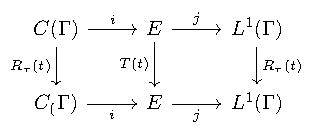
\includegraphics[width=0.5\textwidth]{./tikz-images/tikz-chap-c3-a.pdf}
\end{center}
%% --
% 	\[ 
% 	\begin{tikzcd}
% 		C(\Gamma) \arrow[r, "i"] \arrow[d, "R_\tau(t)"'] & E  \arrow[r, "j"] \arrow[d, "T(t)"'] & L^1(\Gamma) \arrow[d, "R_\tau(t)"] \\
% 		C_(\Gamma) \arrow[r, "i"'] & E \arrow[r, "j"'] & L^{1}(\Gamma)
% 	\end{tikzcd}
% 	\]
% 	%% --
\end{corollary}
%% --
\begin{proof}
    By Theorem~\ref{thm:c3-3.8} and Part-I, Theorem~\ref{thm:a3-5.4} we have $R\sigma(A) = P\sigma(A) = \sigma(A) = \im\alpha\Z$ with $\alpha \coloneq \frac{2\pi}{n\tau}$ for suitable $n \in \N$.
    We fix $h \in \ker(\im\alpha - A)$, $h \neq 0$.
    Then $|h| \in \ker A$ and there exists $\phi \in \ker A'$ such that $\langle|h|,\phi\rangle = 1$.
    According to the Kakutani-Krein Theorem we identify $E_{|h|}$ with $C(K)$.
    Then $h$ is a unimodular function onto $\Gamma$ (use the argument given in the proof of Part-II, Theorem~\ref{thm:b3-3.6}(iii)).
    
    We define $j \colon C(\Gamma) \to E$ by $j(f) \coloneq f\circ h \in C(K) \cong E_{h} \subseteq E$, then $j$ is injective.
    For the monomials $e_{n}(z) \coloneq z^{n}$ $(n \in \Z)$ we have $j(e_{n}) = h^{[n]}$ thus $j$ has dense image in $E$ (by Part-I, Theorem~\ref{thm:a3-5.4}).
    Moreover, 
    \[
    \langle h^{[n]},\phi\rangle = \langle j(e_{n}),\phi\rangle = \int_{0}^{2\pi} e_{n}(\eu^{\im t})\dt  =2\pi\cdot\delta_{n0}\  \text{ for all } n \in \Z , 
    \] 
    hence $\int_{0}^{2\pi} f(\eu^{\im t})\dt   = \langle j(f),\phi\rangle$ for all $f \in C(\Gamma)$.
    
    It follows that $(E,\phi) \cong L^{1}(\Gamma)$, and we define $\tilde{j}$ to be the canonical mapping from $E$ into $(E,\phi) \cong L^{1}(\Gamma)$ (see Section~\ref{sec:c1-4}).
    Then $\tilde{j}$ has dense image and is injective since $\phi$ is strictly positive (\cf Proposition~\ref{prop:c3-3.5}\,(ii)).
    One easily verifies that the diagram commutes.
\end{proof}
%% --
Now we are going to prove the main result of this section.
As in the proof of Theorem~\ref{thm:c3-2.10} we will utilize pseudo-resolvents%
\index{pseudo-resolvent} 
on a suitable $\mathcal{F}$-product%
\index{F-product@$\mathcal{F}$-product}
of the Banach lattice.
To simplify the proof we isolate two lemmas.

%% --
\begin{lemma}\label{lem:c3-3.10}
	
	Let $\mathcal{F}$ be a filter on $\N$ which is finer than the Fréchet filter and let $E_{\mathcal{F}}$ be the $\mathcal{F}$-product of the Banach lattice $E$.
	Given $R \in \mathcal{L}(E)$ and denoting its canonical extension to $E_{\mathcal{F}}$ by $R_{\mathcal{F}}$ the following is true.
\begin{quote}
	If\/ $\alpha \in A\sigma(R)\setminus P\sigma(R)$, then $\ker(\alpha - R_{\mathcal{F}})$ is infinite dimensional.
\end{quote}
\end{lemma}
%% --	
\begin{proof}
    Let $(f_{n})_{n\geq 1}$ be a normalized approximate eigenvector of\/ $R$ corresponding to $\alpha$.
    Since every accumulation point of\/ $(f_{n})$ is an eigenvector of\/ $R$, the assumption $\alpha \notin P\sigma(A)$ implies that $(f_{n})$ does not have any accumulation points.
    Then there exist an $\epsilon > 0$ and a subsequence $(g_{n})$ of\/ $(f_{n})$ such that
    %% --
    \begin{equation}\label{eq:c3-3.14}
        \|g_{n} - g_{m}\| \geq \epsilon \text{ whenever } n \neq m.
    \end{equation}
    %% --
  
    Obviously, $(g_{n})$ is a normalized approximate eigenvector of\/ $R$ and so is every subsequence of\/ $(g_{n})$.
    In particular, for $k \in \N$ the sequence $(g_{n+k})_{n\geq 1}$ is a normalized approximate eigenvector of\/ $R$.
    Then the elements $\hat{g}^{k} \in E_{\mathcal{F}}$ given by $\hat{g}^{k} \coloneq ((g_{n+k})_{n\geq 1} + c_{\mathcal{F}}(E))$ are normalized eigenvectors of\/ $R_{\mathcal{F}}$ corresponding to $\alpha$.
    As a consequence of Eq.~\myeqpageref{eq:c3-3.14} we obtain
    %
\[
	\|\hat{g}^{k} - \hat{g}^{m}\| = \mathcal{F}\text{-}\lim\sup\|g_{n+k} - g_{n+m}\| \geq \epsilon
\]
%
provided that $k \neq m$.
    This shows that the unit ball in $\ker(\alpha - R_{\mathcal{F}})$ is not relatively compact, hence $\ker(\alpha - R_{\mathcal{F}})$ has to be infinite dimensional.
\end{proof}
%% --
%% --
\begin{lemma}\label{lem:c3-3.11}
	
	Let $E$ be a Banach lattice and let $M$, $L$ be two linear subspaces of\/ $E$.
	Assume that $f \in M$ implies $|f| \in L$, then $\dim L \geq \dim M$.
\end{lemma}
%% --	
\begin{proof}
    Let $\{g_{1},g_{2},\ldots,g_{m}\}$ $(m\geq 1)$ be any (finite) subset of\/ $M$ which is linearly independent.
    For $u \coloneq \sum_{n=1}^{m}|g_{n}|$ all vectors $g_{n}$ are contained in the principal ideal $E_{u}$ which (by the Kakutani-Krein Theorem) is isomorphic to a space $C(K)$.
    Considering $g_{1}$, $g_{2}$, $\ldots$, $g_{m}$ as continuous functions on $K$, there exist points $x_{1}$, $x_{2}$, $\ldots$, $x_{m} \in K$ and functions $h_{1}$, $h_{2}$, $\ldots$, $h_{m} \in \mathrm{span}\{g_{1},g_{2},\ldots,g_{m}\}$ such that $h_{i}(x_{j}) = \delta_{ij}$.
    Then $|h_{i}|(x_{j}) = \delta_{ij}$ hence $\{|h_{j}| \colon 1\leq j\leq m\}$
    is a subset of\/ $m$ linearly independent vectors which (by assumption) is contained in $L$.
\end{proof}
%% --
The surprising fact in the following theorem is the conclusion that every point in the boundary spectrum is a simple algebraic pole 
\index{resolvent!algebraically simple pole}
if only $s(A)$ is supposed to be a pole.

%% --
\begin{theorem}\label{thm:c3-3.12}
\index{resolvent!pole}

Let $\TT$ be an irreducible semigroup on a Banach lattice and let $A$ be its generator.
If\/ $s(A)$ is a pole of the resolvent, then $\sigma_{b}(A) = s(A) + \im\alpha\Z$ for some $\alpha \geq 0$.
Moreover, $\sigma_{b}(A)$ contains only algebraically simple poles.
\end{theorem}
\index{irreducible semigroup|)}
\index{semigroup!irreducible semigroup|)}

%% --
\begin{proof}
	We will assume that $s(A) = 0$.
	Assuming first that every element of\/ $\sigma_{b}(A)$ is an eigenvalue of\/ $A$, one can conclude the following.
	By Theorem~\ref{thm:c3-3.8}\,(i) we know that $\sigma_{b}(A)$ is an additive subgroup of\/ $\im\R $.
	Since it is a closed subset and $0$ is an isolated point, it follows that $\sigma_{b}(A) = \im\alpha\Z$ for some $\alpha \geq 0$.
	Moreover, as a consequence of Eq.~\myeqpageref{eq:c3-3.13}, for every $k \in \Z$ we obtain
	%% --
	\begin{equation}\label{eq:c3-3.15}
		R(\lambda+\im k\alpha,A) = S_{h}^{-k}\circ R(\lambda,A)\circ S_{h}^{k} \quad (\lambda \in \rho(A),\, k \in \Z).
	\end{equation}
	%% --
	
	By Proposition~\ref{prop:c3-3.5}\,(iv) $0$ is an algebraically simple pole.
	Then Eq.~\myeqpageref{eq:c3-3.15} implies that every point $\im k\alpha$ has the same property.
	
	We now show that every element $\im\beta$ is an eigenvalue of\/ $A$.
	By Proposition~\ref{prop:c3-3.5}\,(iv) the residue of\/ $R(\cdot,A)$ in $\lambda = 0$ has the form $P = \phi\otimes u$ with $\phi(u) = 1$.
	Given an ultrafilter $\mathcal{U}$ on $\N$ which is finer than the Fréchet filter, then $\lim_{\mathcal{U}}\phi(f_{n})$ exists for every bounded sequence $(f_{n})$ in $E$.
	Using this fact it is easy to see that the canonical extension $P_{\mathcal{U}}$ of\/ $P$ to the $\mathcal{U}$-product $E_{\mathcal{U}}$ of\/ $E$ has the following form.
	%% --
\begin{equation}\label{eq:c3-3.16}
\begin{split}
		&P_{\mathcal{U}} = \hat{\phi}\otimes\hat{u} \text{ where } \hat{u} \coloneq (u,u,u,\ldots)+c_{\mathcal{U}}(E) \in E_{\mathcal{U}} \ \text{ and } \hat{\phi} \in (E_{\mathcal{U}})'
		\\
		&\text{is given by } \hat{\phi}((f_{n})+c_{\mathcal{U}}(E)) \coloneq \lim_{\mathcal{U}}\phi(f_{n}) \ ((f_{n})+c_{\mathcal{U}}(E) \in E_{\mathcal{U}}) .
		\end{split}
	\end{equation}
	%% --
	
	Given $\im\beta \in \sigma_{b}(A)$ then $\im\beta \in A\sigma(A)$ hence $1 \in A\sigma(\lambda R(\lambda+\im\beta,A))$.
	If we assume that  $\im\beta \notin P\sigma(A)$, then $1 \notin P\sigma(\lambda R(\lambda+\im\beta,A))$.
	Then Lemma~\ref{lem:c3-3.10} implies that 
	%
\[
	M \coloneq \ker(1 - \lambda R(\lambda+\im\beta,A)_{\mathcal{U}})
\]
%
is infinite dimensional (and independent of\/ $\lambda$ by Proposition~\ref{prop:c3-2.6}\,(i).)

For $\hat{f} \in M$ we have 
%
\[
	|\hat{f}| = \gamma R(\gamma+\im\beta,A)_{\mathcal{U}}|\hat{f}| \leq \gamma R(\gamma,A)_{\mathcal{U}}|\hat{f}|
\]
%
for every $\gamma > 0$.
It follows that 
%
\[
	\hat{\phi}(|\hat{f}|) = P_{\mathcal{U}}|\hat{f}| = \lim_{\gamma\to 0}\gamma R(\gamma,A)_{\mathcal{U}}|\hat{f}| \geq |\hat{f}| .
\]
%
Thus considering the closed ideal $I \coloneq \{\hat{f} \in E_{\mathcal{U}} \colon \hat{\phi}(|\hat{f}|) = 0\}$ we have
	%% --
	\begin{equation}\label{eq:c3-3.17}
		\tilde{\phi}(|\hat{f}|) - |\hat{f}| \in I \ \text{ for every } \hat{f} \in M .
	\end{equation}
	%% --
	This implies that $M \cap I = \{0\}$. 
	Hence the canonical image $M_/$ of\/ $M$ in the quotient space $E_{\mathcal{U}/{I}}$ is infinite dimensional as well. 
	
	By Eq.~\myeqpageref{eq:c3-3.16} and Eq.~\myeqpageref{eq:c3-3.17} the absolute value of an element $\tilde{f} \in M_/$ is a scalar multiple of\/ $\tilde{u} \coloneq \hat{u} + I$. 
	This is a contradiction by Lemma~\ref{lem:c3-3.11}.
\end{proof}
%% --
In view of Part-I, Proposition~\ref{prop:a3-4.2} the result above has consequences for semigroups which can be reduced (by considering restrictions to invariant ideals or quotients) to semigroups which satisfy the hypothesis of Theorem~\ref{thm:c3-3.12}. 
Semigroups having this property are precisely those for which $s(A)$ is a pole of the resolvent of finite algebraic multiplicity. 
The latter claim is a consequence of Proposition~\ref{prop:c3-2.11} and the following lemma.
%% --
\begin{lemma}\label{lem:c3-3.13}
	Suppose that $\TT = (T(t))_{t  \geq 0}$ is a positive semigroup such that $s(A)$ is a first order pole of the resolvent. 
	Moreover assume that the corresponding residue is a strictly positive operator of finite rank.
%% --	
	Then there are closed $\TT$-invariant ideals $J_{1},J_{2}, .. J_{m}$ which are mutually orthogonal. 
	For the restrictions  $\TT_{k}$ of\/ $\TT$ to $J_{k}$ the following is true.
    %% --
    \index{spectral bound $s(A)$}
	\begin{enumerate}[\upshape (i)]
		\item $\TT_{k}$ is irreducible with spectral bound $s(A_k) = s(A)$. 
		\item $s(A_{/J}) < s(A)$  where $J \coloneq  J_{1}\oplus J_{2}\oplus .. \oplus J_{m} .$
	\end{enumerate}
\end{lemma}
%% --
\begin{proof}
We assume $s(A) = 0$. 
Since $P$ is a strictly positive projection $PE = \ker A$ is a sublattice of\/ $E$. 
Actually, if\/ $x \in PE$ \ie  $Px = x$, then $P|x| \geq |Px| = |x|$. 
Hence 
%
\[
	P(|P|x|-|x||) = P^{2}|x| - P|x| = 0
\]
%
which implies that $P|x| - |x| = 0$ or $|x| \in PE$.
Thus we know that $\ker A$ is a finite dimensional sublattice of\/ $E$ hence it is isomorphic to a space $\C ^{m}$ for some $m \in \N$ (see Section~II.4 of \textcite{schaefer:1974}). 
	
Then there exist vectors $e_{j} \in E_{+}$ $(1\leq j\leq m)$ such that the following holds.
%% --
\begin{equation}\label{eq:c3-3.18}
	\ker A = \mathrm{span} \{e_{1},e_{2}, \ldots ,e_{m}\} \text{ and } \inf\{e_{i},e_{j}\} = 0 \ \text{ for }  i \neq j .
\end{equation}
%% --
We have $T(t)e_{k} = e_{k}$ hence the closed ideal generated by $e_{k}$ is $\TT$-invariant. 
We denote this ideal $J_{k}$ and define $J\coloneq  J_{1}\oplus J_{2}\oplus \ldots \oplus J_{m}$.
The ideal $J$ is closed, $\TT$-invariant and we have $PE = \ker A \subseteq J$ (see \textcite[III Theorem~1.2]{schaefer:1974}). 
Then $P_{/J} = 0$ hence the spectral bound $s(A_{/J})$
	is strictly less than zero (by Theorem~\ref{thm:c3-1.1}\,(i)). 
	Moreover, the residue corresponding to the resolvent of\/ $\TT_{k}$, we denote it $P_{k}$, is the restriction of\/ $P$ to $J_{k}$.
	
	Then $P_{k}$ is strictly positive and $P(J_{k}) = \mathrm{span}\{e_{k}\}$. 
	To show that $T_{k}$ is irreducible, we consider an invariant ideal $I$. 
	Then we have $R(\lambda,A_{k})I \subseteq I$ for $\lambda > 0$ hence $P_{k} = \lim_{\lambda \to 0}\lambda R(\lambda,A_{k})$ leaves $I$ invariant. 
	If\/ $I \neq \{0\}$, then $P_{k}I \neq \{0\}$ since $P_{k}$ is strictly positive. 
\end{proof}
%% --
Combining the lemma with Proposition~\ref{prop:c3-2.11} one obtains the following.

If\/ $s(A)$ is a pole of finite algebraic multiplicity, then there exists a finite chain of\/ $\TT$-invariant ideals $I_{-1} \coloneq  \{0\} \subseteq I_{0}\subseteq \ldots \subseteq I_{N} \coloneq  E$ $(N\in\N)$ such that the following is true.
%% --
\begin{equation}\label{eq:c3-3.19}
	\begin{split}
	&\textit{For the semigroup $\TT_{n}$ on $I_{n}/I_{n-1}\, \ (0 \leq n \leq N)$ which is induced by $\TT$}
		\\
	& \textit{we have either $s(A_{n}) = s(A)$ and $\TT_{n}$ is irreducible or $s(A_{n}) < s(A)$} .
	\end{split}
\end{equation}
%% --
The following theorem is an immediate consequence of Eq.~\myeqpageref{eq:c3-3.19}, Theorem~\ref{thm:c3-3.12} and Part-I, Proposition~\ref{prop:a3-4.2}.
%% --
\begin{theorem}\label{thm:c3-3.14}
\index{resolvent!pole}%
\index{boundary spectrum}
	Let $\TT$ be a positive semigroup on a Banach lattice with generator $A$. 
	If\/ $s(A)$ is a pole of finite algebraic multiplicity, then $\sigma_{b}(A)$ is a finite union of discrete subgroups, \ie  
%
\[
		\sigma_{b}(A) = s(A) + \bigcup_{k=1}^{N}\im\alpha_{k}\Z \text{ with $\alpha_{k} \in \R$.}
\]
%
Moreover, $\sigma_{b}$ contains only poles of finite algebraic multiplicity.
\end{theorem}
%% --
Here the assumption that the multiplicity of\/ $s(A)$ is finite is essential as can be seen from the following example.
%% --
\begin{example}\label{ex:c3-3.15}
	Consider $X \coloneq  [0,1] \times V$, $V \coloneq  \{v \in \R  \colon v_{1} < |v| < v_{2}\}$ $(0 < v_{1} < v_{2} < \infty)$. 
	The flow in the phase space $X$ which describes the free motion in the interval $[0,1]$ with velocities in $V$ assuming that the particles are reflected at the endpoints generates a positive semigroup on $L^{p}(X,\mu)$ $(\mu$ the Lebesgue measure). 
	For the spectrum of the generator $A$ one obtains 
    \[
    \sigma(A) = \{\im \gamma \colon n\gamma_{1} \leq |\gamma| \leq n\gamma_{2} \text{ for some } n \in \N_{0}\}
    \]
    with $\gamma_{1} \coloneq  \pi/v_{1}$, $\gamma_{2} \coloneq  \pi/v_{2}$. 
	Moreover, $0$ is a first order pole of the resolvent, obviously the only pole in $\sigma_{b}(A) = \sigma(A)$.
	These statements can be verified by calculating the resolvent explicitly. 
	This can be done using the integral representation. 
    The semigroup is given as follows.
%% --
\begin{equation}\label{eq:c3-3.20}
	\textit{\small $
	(T(t)f)(x,v) = \begin{cases}
		f(x-vt+k,v) & \text{if } k-1\leq vt-x\leq k \text{ and } k \textit{ even}, \\
		f(1-(x-vt+k),-v) & \text{if } k-1\leq vt-x\leq k \text{ and } k \text{ odd}.
	\end{cases}
$}
\end{equation} 

Obviously one can apply Theorem~\ref{thm:c3-3.12} and Theorem~\ref{thm:c3-3.14}, respectively, in order to prove existence of strictly dominant eigenvalues. 
We consider two typical cases in the following corollaries. 
The meaning of\/ $r_{ess}(T(t))$ and $\omega_{ess}(\TT)$ and its properties are explained in Part-I, Example~\ref{ex:a3-3.7}.
\end{example}
%% --
\begin{corollary}\label{cor:c3-3.16}
    \index{spectrum!essential}
    \index{quasi-interior point}
	Suppose that $\TT$ is a positive semigroup such that $\omega_{ess}(\TT) < \omega_0(\TT)$. 
	Then $s(A) = \omega_0(\TT)$ is a strictly dominant eigenvalue.
	If, in addition, there exists an eigenfunction which is a quasi-interior point of\/ $E_{+}$ (\eg if\/ $\TT$ is irreducible), then $s(A)$ is a first order pole of\/ $R(.,A)$.
\end{corollary}
%% --
\begin{proof}
	There exist $\epsilon > 0$ such that 
    %for every $t > 0 the set 
    $\{\lambda \in \sigma(T(t)) \colon |\lambda| \geq \exp((s(A)-\epsilon)t)\}$ contains only (finitely many) poles of\/ $R(\cdot,T(t))$ each being of finite algebraic multiplicity. 
	In view of Part-I, Corollary~\ref{cor:a3-6.5} the set $\{\lambda \in \sigma(A) \colon \Re(\lambda) > s(A)-\epsilon\}$ is finite and contains only poles of\/ $R(\cdot,A)$. 
	Thus we can apply Theorem~\ref{thm:c3-3.14}. 
	It follows that $s(A)$ is strictly dominant.
	For the final assertion we refer to Remark~\ref{rem:c3-2.15}\,(ii).
\end{proof}
%% --
\begin{corollary}\label{cor:c3-3.17}
	Suppose that $\TT$ is an irreducible, eventually norm continuous semigroup having compact resolvent.
	Then $s(A) = \omega_0(\TT)$ is an algebraically simple pole and a strictly dominant eigenvalue.
    \index{resolvent!algebraically simple pole}
\end{corollary}
%% --
\begin{proof}
	By Theorem~\ref{thm:c3-3.7}\,(iii) we know that $s(A) > -\infty$. 
	Theorem~\ref{thm:c3-3.12} is applicable since we assumed that $\TT$ is irreducible and has compact resolvent.
	Thus $s(A)$ is an algebraically simple pole and $\sigma_{b}(A) = s(A) + \im\alpha\Z$ for some $\alpha \geq 0$. 
	In addition $\{\lambda \in \sigma(A) \colon \Re(\lambda) \geq -1\}$ is compact since $\TT$ is eventually norm-continuous (see Part-I, Theorem~\ref{thm:a2-1.20}). 
	It follows that $s(A)$ is strictly dominant.
	By Part-I, Theorem~\ref{thm:a3-6.6} we have $s(A) = \omega_0(\TT)$.
\end{proof}
 
In the following proposition we give a condition which ensures that Theorem~\ref{thm:c3-3.14} can be applied to certain perturbations. 
Moreover, we state a criterion ensuring the existence of a dominant eigenvalue.
\index{operator!compact}
%% --
\begin{proposition}\label{prop:c3-3.18}
\index{spectral bound $s(A)$!dominant}
Suppose that $A$ is the generator of a positive semigroup and that $K \in \LE$ is a positive linear operator.
%
\begin{enumerate}[\upshape(i)]
\item
If\/ $K$ is $A$-compact, \ie $K\cdot R(\lambda_{0},A)$ is compact for some
$\lambda_{0} \in \rho(A)$, and if\/ $s(A+K) > s(A)$, then
$B \coloneq A + K$ satisfies the assumptions of Theorem~\ref{thm:c3-3.14}.%
\item
If, in addition, $K$ is irreducible, then $s(B)$ is a dominant eigenvalue and the semigroup generated by $B$ is irreducible.
\end{enumerate}
%% --	
\end{proposition}
%% --
\begin{proof}
The resolvent equation %
\[
	R(\lambda,A) = R(\lambda_{0},A)(\Id - (\lambda-\lambda_{0})R(\lambda,A))
\]
%
implies that $K \cdot R(\lambda,A)$ is a compact operator for every $\lambda \in \rho(A)$. 
For $\lambda > s(A)$ we have 
%
\[
	\lambda - B = (\Id - KR(\lambda,A))(\lambda-A)
\]
%
and $(\Id - KR(\lambda,A))^{-1}$ exists for $\lambda > s(B)$.

Therefore \textcite[Theorem XIII.13]{reedsimon:1979} 
implies that %
\[
	R(\lambda,B) = R(\lambda,A)(1 - KR(\lambda,A))^{-1}
\]
%
has only poles of finite algebraic multiplicity in $\{\lambda \in \C  \colon \Re(\lambda) > s(A)\}$. 
This proves the first claim.

In order to prove the second, we denote the semigroup corresponding to $A$ and $B$ by $(T(t))$ and $(S(t))$,  respectively.
It follows from Proposition~\ref{prop:c3-3.3} that $(S(t))$ is irreducible and we have $S(t) = T(t) + \int_{0}^{t} T(t-s)KS(s)\ds$ (see Eq.~\myeqpageref{eq:a2-1.9}). 
Iterating this identity we obtain for every $m \in \N$, $t \geq 0$
%% --
\begin{equation}\label{eq:c3-3.21}
\begin{split}
    S(t) &= \sum_{n=0}^{m-1} T_{n}(t) + R_{m}(t) \ \text{ where}\\ 
    T_{0}(t)&\coloneq T(t),\  T_{n}(t) \coloneq  \int_{0}^{t} T(t-s)KT_{n-1}(s)\ds \text{ for } n \in \N , \\
    R_{m}(t) &\coloneq \textit{\small $\int_{0}^{t}\int_{0}^{t_{1}} \ldots \int_{0}^{t_{m-1}} T(t-t_{1})KT(t_{1}-t_{2})K \ldots T(t_{m-1}-t_m)KS(t_{m})\dt _{m}\ldots \dt _{1}$} .
\end{split}
\end{equation}
%% --
We fix $0 < f \in E$, $0 < \phi \in E'$, $t > 0$. 
By Theorem~\ref{thm:c3-3.2}\,(i), $S(t)f > 0$.
Since $K$ is irreducible, there exists $m \in \N$ such that $\langle K^{m}f,\phi\rangle > 0$. 
Thus the integrand appearing in the representation Eq.~\myeqpageref{eq:c3-3.21} of\/ $\langle R_{m}(t)f,\phi\rangle$ is non-zero at $t_{1}=t_{2}= \ldots =t_{m-1}=t$, $t_{m}= t$.

Since the integrand is positive and continuous, we conclude
\begin{equation}\label{eq:c3-3.22}%\textstyle
    \langle S(t)f,\phi\rangle \geq \langle R_{m}(t)f,\phi\rangle > 0 \ \text{ for } \ 0 < f  ,   \ 0 < \phi \ \text{ and } \ t > 0 .
\end{equation}
%% --
It follows that $(\eu^{-ts(B)}S(t))_{t \geq 0}$ cannot contain the rotation semigroup on $\Gamma$. 
On the other hand, assuming that $s(B)$ is not dominant, then $\dim(\ker((\eu^{\tau\cdot s(B)} - S(\tau))) > 1$ for some $\tau > 0$. 
Hence, the restriction $(\eu^{-ts(B)}S(t)_{|F})_{t \geq 0}$, $F \coloneq  \ker(\eu^{\tau\cdot s(B)}- S(\tau))$, contains the rotation semigroup by Corollary~\ref{cor:c3-3.9}.
\end{proof}
%% --
We conclude this section considering the linear transport equation%
\index{transport equation} 
once again, see Example~\ref{ex:c3-3.4}\,(iv).
The generator considered there is $B = (A - M) + K$, where $K$ is positive linear. 
From Eq.~\eqref{eq:c3-3.5} and Eq.~\myeqpageref{eq:c3-3.6} one deduces that 
%% --
\[
(KR(\lambda,A)f)(x,v) = \int_{0}^{1}\int_{-1}^{1} k(x,v,x',v')f(x',v')\dx'dv'
\]
%% --
where the kernel $k$ is given by $k(x,v,x',v') \coloneq  \kappa(x,v,v')r_{\lambda}(x,x',v')$ (\cf Eq.~\eqref{eq:c3-3.5} and Eq.~\myeqpageref{eq:c3-3.7}). 
Using this representation of\/ $KR(\lambda,A)$ it follows that $K$ is A-compact. 
Moreover for $\lambda$ sufficiently large one has $R(\lambda,A-M) = R(\lambda,A)(1 - MR(\lambda,A))^{-1}$ which shows that $K$ is also $(A-M)$-compact. 
In order to apply Theorem~\ref{thm:c3-3.14} one needs $s(B) > s(A-M)$ (see Proposition~\ref{prop:c3-3.18}) which is difficult to verify. 
In case the function $\sigma$ is continuous one can state a sufficient condition as follows.
There exist $r \in \R $ and $g \in L^{1}([0,1]\times[-1,1])$, $g > 0$ such that $r < \inf\{\sigma(x,0) \colon x \in [0,1]\}$ and $Bg \geq -rg$.
The additional assumption made in the second part of Proposition~\ref{prop:c3-3.18} is not satisfied in this example. 
Nevertheless one can show that $s(B)$ is strictly dominant in this situation (provided that $s(B) > s(A)$). 
For details we refer to \textcite{greiner:1984d}  or \textcite{voigt:1985} where the linear transport equation in higher dimensional spaces is discussed.
%% --
\section{Semigroups of Lattice Homomorphisms}\label{sec:c3-4}
\index{lattice homomorphism|(}
\index{spectrum!lattice semigroup}
\index{semigroup!lattice semigroup} 
%% --
In Section~\ref{sec:c3-2} we proved that the boundary spectrum of certain positive semigroups is a cyclic set. 
For semigroups of lattice homomorphisms much more can be said. 
The whole spectrum is an imaginary additively cyclic subset of\/ $\C $ (\cf Theorem~\ref{thm:c3-4.2}). 
This result can be used to derive cyclicity results for the eigenvalues in the boundary spectrum of positive semigroups (\cf Corollary~\ref{cor:c3-4.3}). 
In the last part of this section we discuss a spectral decomposition of positive groups (\cf Theorem~\ref{thm:c3-4.8}).
%% --
\begin{lemma}\label{lem:c3-4.1}
	Suppose that $(T(t))_{t  \geq 0}$ is a semigroup of lattice homomorphisms on a Banach lattice $E$ with generator $A$.
	In case $\im\alpha \in R\sigma(A)$, $\alpha \in \R $, then one of the following assertions are true
	\begin{enumerate}[\upshape (a)]
		\item $\im\alpha\Z \subseteq R\sigma(A)$;
		\item $\{\lambda \in \C  \colon \Re(\lambda) < 0 \} \subseteq R\sigma(A)$.
	\end{enumerate}
\end{lemma}
%% --
\begin{proof}
	There exists $\phi \in E'$, $\phi \neq 0$ such that $T(t)'\phi = \eu^{\im\alpha t}\phi$ $(t \geq 0)$. 
	Then we have $|\phi| = |T(t)'\phi| \leq T(t)'|\phi|$ $(t \geq 0)$.
	If we fix $r > \omega_0(\TT)$ and define $\psi \coloneq  rR(r,A)'|\phi|$, we have
	%% -- 
	\begin{equation}\label{eq:c3-4.1}
		T(t)'\psi \leq \eu^{rt}\psi \ \text{ and } \ \ T(t)'\psi \geq \psi \ (t \geq 0) \ \text{ and } \ |\phi| \leq \psi .
	\end{equation}
	%% --
	In fact, Eq.~\myeqpageref{eq:a1-3.1} implies $(\eu^{rt} - T(r))R(r,A) \geq 0$ hence 
    \[
    T(t)'\psi = rR(r,A)'T(t)'|\phi| \leq r\cdot \eu^{rt}R(r,A)'|\phi| = \eu^{rt}\psi .
    \]
	Moreover, the inequality $T(t)'|\phi| \geq |\phi|$ $(t \geq 0)$ implies 
    \[
    T(t)'\psi = rR(r,A)'T(t)'|\phi| \geq rR(r,A)'|\phi| = \psi
    \]
    and 
    \[
    \psi = rR(r,A)'|\phi| = r \int_{0}^{\infty} \eu^{-rt}T(t)'|\phi|\dt  \geq r\int_{0}^{\infty} \eu^{-rt}|\phi|\dt  = |\phi| .
    \]
    %% --
	Now, considering the AL-space $(E,\psi)$ (see Section~\ref{sec:c1-4}) the first inequality of Eq.~\myeqpageref{eq:c3-4.1} implies that $(T(t))_{t \geq 0}$ induces a strongly continuous semigroup $(T_{1}(t))_{t \geq 0}$ on $(E,\psi)$.
	That is we have
	%% --
	\begin{equation}\label{eq:c3-4.2}
    %\textstyle
		T_{1}(t)\circ q_{\psi} = q_{\psi}\circ T(t) \ (t \geq 0) .
	\end{equation}
	%% -- tikz
\begin{center}
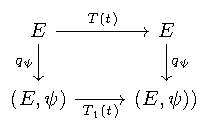
\includegraphics[width=0.4\textwidth]{./tikz-images/tikz-chap-c3-b.pdf}
\end{center}
% 	\[
% 	\begin{tikzcd}
% 		E \arrow[r, "T(t)"] \arrow[d, "q_\psi"'] & E \arrow[d, "q_\psi"] \\
% 		(E,\psi) \arrow[r, "T_1(t)"'] & (E,\psi))
% 	\end{tikzcd}
% 	\]
	%% --
	Denoting by $A_{1}$ the generator of\/ $(T_{1}(t))$ we have $R\sigma(A_{1}) \subseteq R\sigma(A)$.
	Indeed, assuming $A_{1}^*x = \lambda x$ then $T_{1}(t)'x = \eu^{\lambda t}x$, hence  $T(t)'q_{\psi}'(x) = \eu^{\lambda t}q_{\psi}'(x)$ (by Eq.~\myeqpageref{eq:c3-4.2}) or equivalently, $A^*(q_{\psi}'(x)) = q_{\psi}'(x)$. 
	Thus it remains to show that either $\im\alpha\Z$ or $\{\lambda \in \C  \colon \Re(\lambda) < 0 \}$ is contained in $R\sigma(A_{1})$. 
	
	Obviously, $(T_{1}(t))$ is a semigroup of lattice homomorphisms as well. 
	The second inequality of Eq.~\myeqpageref{eq:c3-4.1} implies
	%% --
	\begin{equation}\label{eq:c3-4.3}
	\|T_{1}(t)f\|_{\psi} = \langle|T_{1}(t)f|,\psi\rangle = \langle|f|,T_{1}(t)'\psi\rangle \geq \langle|f|,\psi\rangle = \|f\|_{\psi} .
	\end{equation}
	%% --
	Then for $\lambda \in \C $ with $\Re(\lambda) < 0$ we have 
	\[ 
	\|(\eu^{\lambda t}-T_{1}(t))f\|_{\psi} \geq \|T_{1}(t)f\|_{\psi}-\|\eu^{\lambda t}f\|_{\psi} \geq (1-|\eu^{\lambda t}|)\|f\|_{\psi} \ (f \in (E,\psi))
	\]
	and we obtain for the corresponding generator
	%% --
	\begin{equation}\label{eq:c3-4.4}
		\begin{split}
		\|(\lambda-A_{1})f\|_{\psi} &= \lim_{t \to 0}\left\|\frac{1}{t}(\eu^{-\lambda t}T_{1}(t)f-f)\right\|_{\psi} \geq \lim_{t \to 0}\frac{1}{t}(\eu^{-t\Re(\lambda)}-1)\|f\|_{\psi}\\
		&= -\Re(\lambda)\cdot\|f\|_{\psi} \ \text{ for } \ \Re(\lambda) < 0 \ \text{ and } \ f \in (E,\psi) .
		\end{split}
	\end{equation}
	%% --
	It follows from Eq.~\myeqpageref{eq:c3-4.3} and Eq.~\myeqpageref{eq:c3-4.4} that $A\sigma(T_{1}(t))\cap\{z \in \C  \colon |z| < 1\} = \emptyset$ and that $A\sigma(A_{1})\cap\{\lambda \in \C  \colon \Re(\lambda) < 0\} = \emptyset$. 
	Since the topological boundary of the spectrum is always contained in the approximate point spectrum (see Part-I, Proposition~\ref{prop:a3-2.2}) and 
    \index{approximate point spectrum $A\sigma$}
    $R\sigma(T(t))\backslash\{0\} = \exp(tR\sigma(A))$ (see Part-I, Theorem~\ref{thm:a3-6.3}), precisely one of the following two cases occurs.
	\begin{enumerate}[\upshape (A)]
		\item
		$\{\lambda \in \C  \colon \Re(\lambda) < 0\} \subseteq \rho(A_{1})$ and $\{z \in \C  \colon |z| < 1\} \subseteq \rho(T_{1}(t))$;
		
		\item
		$\{\lambda \in \C  \colon \Re(\lambda) < 0\} \subseteq R\sigma(A_{1})$ and $\{z \in \C  \colon |z| < 1\} \subseteq R\sigma(T_{1}(t))$.
	\end{enumerate}
	
	We mentioned above that $R\sigma(A_{1}) \subseteq R\sigma(A)$. 
	Thus we only have to analyze case (A). 
	In this case each operator $T_{1}(t)$ is an invertible lattice homomorphism hence a lattice isomorphism. 
	It follows that $T_{1}(t)'$ is a lattice isomorphism as well. 
	The third inequality in Eq.~\myeqpageref{eq:c3-4.1} implies that $\phi$ can be considered as an element of\/ $(E,\psi)'$ and $T(t)'\phi = \eu^{\im\alpha t}\phi$ $(t \geq 0)$ implies $T_{1}(t)'\phi = \eu^{\im\alpha t}\phi$. 
	Furthermore, we have
	$T_{1}(t)'|\phi| = |T_{1}(t)'\phi| = |\eu^{\im\alpha t}\phi|$ or equivalently $A_{1}^*|\phi| = 0$.
	Now we can apply 
	Theorem~\ref{thm:c3-2.2} 
	and obtain $\im\alpha\Z \subseteq P\sigma(A_{1}^*) = R\sigma(A_{1})$.
	\end{proof}
%% --
\begin{theorem}\label{thm:c3-4.2}
    \index{semigroup!lattice semigroup} 
    \index{spectrum!point spectrum $P\sigma$}
    \index{spectrum!cyclic} 
	Let $A$ be the generator of a semigroup $(T(t))_{t \geq 0}$ of lattice homomorphisms on a Banach lattice $E$. 
	Then $\sigma(A)$, $A\sigma(A)$ and $P\sigma(A)$ are imaginary additively cyclic subsets of\/ $\C $.
\end{theorem}
%% --
\begin{proof}
	We first consider the point spectrum. 
	If\/ $\lambda \in P\sigma(A)$, $\lambda = \alpha + \im\beta$ $(\alpha,\beta \in \R )$, then there exists $f \in E$, $f \neq 0$ such that $Af = \lambda f$. 
	It follows that $T(t)f = \eu^{\lambda t}f$ $(t \geq 0)$ hence $T(t)|f| = |T(t)f| = \eu^{\alpha t}|f|$ $(t \geq 0)$, or equivalently, $A|f| = \alpha|f|$. 
	Now Theorem~\ref{thm:c3-2.2} is applicable and we obtain $A(f^{[n]}) = (\alpha + \im n\beta)f^{[n]}$ for all $n \in \Z$.
	
	To prove the assertion for $A\sigma(A)$ we consider an $\mathcal{F}$-product semigroup%
    \index{semigroup!F-product@$\mathcal{F}$-product}%
    \index{F-product@$\mathcal{F}$-product}
    in order to reduce the problem to the point spectrum. 
	We use the notation of Part-I, Section~\ref{subsec:a1-3.7}. 
	Obviously the space $m(E)$ is a Banach lattice and every operator $\hat{T}(t)$ is a lattice homomorphism. 
	We have %
\[
	|T(t)|f| - |f|| = ||T(t)f| - |f|| \leq |T(t)f - f| \quad (f \in E) ,
\]
%
hence $(|f_{n}|) \in m^{\TT}(E)$ whenever $(f_{n}) \in m^{\TT}(E)$. 
	This proves that $m^{\TT}(E)$ is a sublattice, hence a Banach lattice as well. 
	Obviously, $c_{\mathcal{F}}(E)\cap m^{\TT}(E)$ is an order ideal. 
	Thus $E_{\mathcal{F}}^{\TT}$ is a Banach lattice and $(T_{\mathcal{F}}(t))$ is a semigroup of lattice homomorphisms. 
	It follows that $P\sigma(A_{\mathcal{F}})$ is cyclic, hence $A\sigma(A)$ is cyclic by Part-I, Proposition~\ref{prop:a3-4.2}.
Cyclicity of the entire spectrum follows from the cyclicity of\/ $A\sigma(A)$ and Lemma~\ref{lem:c3-4.1}.
\end{proof}
%% --
One can use Theorem~\ref{thm:c3-4.2} in order to prove cyclicity for the eigenvalues in the boundary spectrum of positive semigroups. 
We list some typical cases in the following corollary.
%% --
\begin{corollary}\label{cor:c3-4.3}
	Let $\TT = (T(t))_{t \geq 0}$ be a positive semigroup on a Banach lattice $E$ which is bounded. 
	Each of the following conditions implies that $P\sigma(A)\cap i\R $ is imaginary additively cyclic.
	\begin{enumerate}[\upshape (i)]
		\item E is weakly sequentially complete (\eg $E = L^{p}(\mu)$, $1 \leq p < \infty$);
		\item Every operator $T(t)$ is mean ergodic (\ie the Cesàro means $\frac{1}{n}\sum_{k=0}^{n-1}T(t)^{k}$ converge strongly as $n \to  \infty$);
		\item There is a strictly positive linear form which is $\TT$-invariant.
	\end{enumerate}
\end{corollary}
%% --
\begin{proof}
	We will show that each of the conditions (i), (ii), (iii) implies that $\ker(1 - T(s))$ is a Banach lattice (not necessarily a sublattice of\/ $E$) for every $s \geq 0$. 
	Then one argues as follows. Given $\im\alpha \in P\sigma(A)$, $\alpha \in \R $, then $T(t)g = \eu^{\im\alpha t}g$ for suitable $g \neq 0$. 
	For $\tau \coloneq  2\pi|\alpha|^{-1}$ we have $g \in F \coloneq  \ker (1 - T(\tau))$. 
	Then the restriction $(T(t)_{|F})_{t \geq 0}$ is a $\tau$-periodic positive semigroup on $F$. 
	Since $\left(T(t)_{|F}\right)^{-1} = T(n\tau-t)_{|F} \geq 0$, it follows that $(T(t)_{|F})$ is a semigroup of lattice isomorphisms. 
	Since $g \in F$, we have $\im\alpha \in P\sigma(A_{|F})$ hence $\im\alpha\Z \in P\sigma(A_{|F}) \subseteq P\sigma(A)$ by Theorem~\ref{thm:c3-4.2}.
	
	Now we show that $\ker (1 - T(s))$ is a vector lattice for the induced order and a Banach lattice for an equivalent norm.
	
	In case (iii), $\ker (1 - T(s))$ is even a sublattice of\/ $E$. 
	Indeed, assume $T(t)'\phi = \phi$ and $\phi \gg 0 ,  (t \geq 0)$, then $T(s)f = f$ implies $T(s)|f| \geq |f|$. 
	Thus from 
	%
\[
	\langle T(s)|f| - |f|,\phi\rangle = \langle |f|,T(s)'\phi - \phi \rangle = 0
\]
%
it follows that $T(s)|f| = |f|$.
	
	Now we assume that $E$ is weakly sequentially complete, which is equivalent to (\cf Section~\ref{sec:c1-5})
	%% --
\begin{equation}\label{eq:c3-4.5}
	\textit{Every increasing norm-bounded net of\/ $E_{+}$ converges}.
\end{equation}
	%% --
	We fix $s > 0$ and define $T \coloneq  T(s)$ and $F \coloneq  \ker (1 - T)$. 
	Obviously $f \in F$ implies $\bar{f} \in F$ hence $F = F\cap E_{\R } + iF\cap E_{\R }$. 
	Thus we have to show that $F_{\R } = F\cap\mathbb{E}_{\R }$ is a sublattice. 
	Given $f \in F_{\R }$, then $Tf = f$ hence $|f| \leq T|f|$. 
	Iterating this inequality we obtain $|f| \leq T|f| \leq T^{2}|f| \leq T^{3}|f| \leq \ldots$.
	By Eq.~\myeqpageref{eq:c3-4.5} $|f|_{o} \coloneq  \lim_{n\to \infty} T^{n}|f|$ exists and we have $T|f|_{o} = \lim_{n\to \infty} T^{n+1}|f| = |f|_{o}$, \ie $|f|_{o} \in F_{\R }$.
	And, for $g \in F_{\R }$ satisfying $\pm f \leq g$, we have $|f|_{o} \leq g$ thus $|f|_{o} = \sup_{F}\{f,-f\}$. 
	Moreover, $\|f\|_{o} \coloneq  \||f|_{o}\|$ $(f \in F)$ is an equivalent norm on $F$ such that $(F,\|\cdot\|_{o})$ is a Banach lattice.
	
	(ii) If\/ $T(s)$ is mean-ergodic, then we have $\ker (1 - T(s)) = PE$ where $P$ is the mean-ergodic projection, \ie $Pf = \lim_{n\to \infty}\frac{1}{n}\sum_{k=0}^{n-1}T(s)^{k}f$.
	Obviously $P$ is positive, hence II.11.5 of \textcite{schaefer:1974} implies that $PE$ is a Banach lattice (for the induced order and an equivalent norm).
\end{proof}
%% --
The assumptions made in Corollary~\ref{cor:c3-4.3} can be weakened slightly (\cf \textcite{greiner:1982}). 
However, one still cannot prove cyclicity of\/ $P\sigma_{b}(A)$ for arbitrary positive semigroups.
%% --
\begin{example}\label{ex:c3-4.4}
	At first we recall Part-II, Example~\ref{ex:b3-2.13}. 
	There we constructed a bounded semigroup on $C(\Gamma)\times C_{0}(\R )$ such that $P\sigma_{b}(A) = \{\im k \colon k \in \Z, k \neq 0\}$.

    Let us perform the same construction on the Hilbert space
    $H \coloneq L^2(\Gamma)\times L^2(\R )$.
    For a fixed positive, non-zero function $k \in C_c(\R )$,
    we define $T(t)$ on $H$ as follows.
    %% --
\begin{equation}\label{eq:c3-4.6}
	\begin{split} 
		T(t)([f,g]) &\coloneq [f_t,g_t] \quad \ \text{with}\\
		f_t(z) &\coloneq f(z \cdot \eu^{\im t}) \quad (z \in \Gamma) \quad \text{and}\\
		g_t(x) &\coloneq g(x+t) + \frac{1}{2\pi}\int_{0}^{2\pi} f(z \cdot \eu^{\im s}) \ds  \cdot \int_{x}^{x+t} k(u) \du  .
	\end{split}
\end{equation}
%% --
Then $(T(t))_{t \geq 0}$ is a positive semigroup on $H$ and for the spectrum of
the generator we obtain $\sigma(A) = i\R $, $P\sigma(A) = i\R \backslash\{0\}$.
In view of Corollary~\ref{cor:c3-4.3}\,(i) the semigroup cannot be bounded.
(The explicit representation Eq.~\myeqpageref{eq:c3-4.6} only allows the estimate $\|T(t)\| \leq \sqrt{2} + t \cdot \|k\|_2$ $(t\geq 0)$.)
\end{example}
%% --
In the next proposition we show that for semigroups of lattice homomorphisms on $L^1$-spaces, there is a spectral mapping theorem for the real part of the spectrum.
\index{spectral mapping theorem}
\index{spectrum!lattice semigroup}
%% --
\begin{proposition}\label{prop:c3-4.5}
\index{spectral mapping theorem!lattice homomorphism}
Let $(T(t))_{t \geq 0}$ be a strongly continuous semigroup
of lattice homomorphisms on an $L^1$-space and denote by $A$ its generator.
Then we have
%% --
\begin{equation}\label{eq:c3-4.7}
	\exp(t\sigma(A) \cap \R ) = \sigma(T(t)) \cap (0,\infty) \quad \text{for every} \quad t \geq 0 .
\end{equation}
%% --
\end{proposition}
%% --
\begin{proof}
In view of Part-I, Proposition~\ref{prop:a3-6.2} it is enough to prove that the left hand
side contains the set on the right.

Fix $t > 0$ and assume $r \in \sigma(T(t))$, $r > 0$ and let $\alpha \coloneq \frac{1}{t} \log r$.
At first we assume $r \in R(\sigma(T(t)))$.
Then by Part-I, Theorem~\ref{thm:a3-6.3} there exists
$\beta \in \R $ such that $\alpha+\im\beta \in R\sigma(A)$.
By Lemma~\ref{lem:c3-4.1} either $\alpha+\im\beta\Z \subseteq R\sigma(A)$
or $\{\lambda \in \C  \colon \Re(\lambda) < \alpha\} \subseteq R\sigma(A)$.
In both cases we have $\alpha \in \sigma(A)$.

Now we assume $r \in A\sigma(T(t))$. 
Then there exists a normalized sequence
$(f_n) \subseteq E$ such that $\lim_{n \to \infty}\|T(t)f_n - rf_n\| = 0$.
Since we have
%% --
\[
|(T(t)|f| - r|f|)| = |(|T(t)f| - r|f|)| \leq |T(t)f - rf|, \  (f \in E) 
\]
%% --
we may assume that $(f_n)$ is a sequence in $E_+$.

Defining $g_n \coloneq \int_{0}^{t} \eu^{-\alpha s}T(s)f_n \ds $ we have $g_n \in D(A)$ and
\[
(A-\alpha)g_n = (A-\alpha)\int_{0}^{t} \eu^{-\alpha s}T(s)f_n \ds = \eu^{-\alpha t}T(t)f_n - f_n = \frac{1}{r}(T(t)f_n - rf_n) .
\]
Therefore $\lim_{n \to \infty}\|(A - \alpha) g_n\| = 0$.  It remains to prove 
$\liminf_{n \to \infty}\|g_n\| > 0$. 
The latter assertion is a consequence of the following facts.
\begin{enumerate}[\upshape (i),wide, labelindent=.25em]

\item
Since $f_n$ is positive and the norm is additive on $E_+$,
we have
\[
    \|g_n\| = \int_{0}^{t} \eu^{-\alpha s}\|T(s)f_n\| \ds .
\]

\item 
The inequality 
\[
    \|T(t)f\| \leq \|T(t-s)\|\|T(s)f\|
\]
%% -- 
implies
%% --
\[
    	\|T(s)f\| \geq M^{-1}\|T(t)f\|
\]
for  $0 \leq s \leq t$, $f \in E$ and $ M \coloneq \sup_{ 0 \leq s \leq t} \|T(s)\|$.
    
    
\item 
Since 
\[
\lim_{n \to \infty} \|T(t)f_{n} - rf_{n}\| = 0 \text{ and $\|f_n\| = 1$}
\]
we have
$\lim_{n \to \infty}\|T(t)f_n\| = r > 0$.
\qedhere
\end{enumerate}
\end{proof}
%% --
For semigroups satisfying the assumption of Proposition~\ref{prop:c3-4.5}, the spectrum $\sigma(A)$ is additively cyclic (by Theorem~\ref{thm:c3-4.2}) and $\sigma(T(t))$ is multiplicatively cyclic
(by \textcite[V.Theorem~4.4]{schaefer:1974}). 
Then the relation Eq.~\myeqpageref{eq:c3-4.7} implies that
decompositions of the spectrum by vertical lines allow a spectral decomposition%
\index{spectral decomposition} 
 of the semigroup (\cf Part-I, Definition~\ref{def:a3-3.1}) (One simply performs a spectral decomposition of a single operator $T(t)$). 

In the following we will show that for positive groups (on arbitrary Banach
lattices) spectral decompositions of this type always exist. 
Moreover,
it will turn out that the decomposition is compatible with the lattice
structure. 
The proof of this result uses Kato's equality (see Section~\ref{sec:c2-5}).% 
\index{Kato's equality} 
As a consequence of Corollary~\ref{cor:c2-5.8}  we have the following.

Let $E$ be a Banach lattice with order continuous norm and $(T(t))_{t \in \R }$
be a group of positive operators on $E$ with generator $A$.
Then the domain $D(A)$ is a sublattice of\/ $E$ and
%% --
\begin{equation}\label{eq:c3-4.8}
	A|f| = \Re [(\text{sign\,} f)Af] \ \text{ for every } \ f \in D(A) , 
\end{equation}
%% --
For real $\mu$ one has $\mu|f| = \Re [(\text{sign } f)\mu f]$, hence
%% --
\[
(\mu - A)|f| = \Re[(\text{sign } f)(\mu - A)f] \ \ \text{ for } \ \mu \in \R , f \in D(A) .
\]
%% --
The relations $f^+ = \frac{1}{2}(|f| + f), \ f^- = \frac{1}{2}(|f| - f)$ yield
%% --
\begin{align*}
(\mu - A)f^+ &= \frac{1}{2}[(\text{sign } f)(\mu - A)f + (\mu - A)f] \quad\ \text{and }\\
(\mu - A)f^- &= \frac{1}{2}[(\text{sign } f)(\mu - A)f - (\mu - A)f] , 
\end{align*}
%% --
in case $f$ is contained in the underlying real Banach lattice $E_{\R }$.
For $\mu \in \rho(A) \cap \R $, we can apply $R(\mu,A)$ on both sides and the substitution $f = R(\mu,A)g$ finally leads to
%% --
\begin{equation}\label{eq:c3-4.9}
	\begin{split}
	(R(\mu,A)g)^+ &= \frac{1}{2}R(\mu,A) [(\text{sign } R(\mu,A)g)g + g] \\
	(R(\mu,A)g)^- &= \frac{1}{2}R(\mu,A) [(\text{sign } R(\mu,A)g)g - g]
	\end{split}
\end{equation}
%% --
for all $g \in E_{\R }$. 
If we set
%% -- 
\[ 
g_1 \coloneq \frac{1}{2}\cdot(g + (\text{sign } R(\mu,A)g)g) \ \text{ and } \ 
g_2 \coloneq \frac{1}{2}\cdot(g - (\text{sign } R(\mu,A)g)g) , 
\]
%% --
then obviously $g = g_1 + g_2$. Moreover, $g$ is positive if and only if
both, $g_1$ and $g_2$ are positive. We summarize these considerations in the following lemma.
%% --
\begin{lemma}\label{lem:c3-4.6}
\index{group of positive operators}
Let $A$ be the generator of a positive group on a Banach
lattice $E$ which has order continuous norm. Given $\mu \in \rho(A) \cap \R $, then
every $g \in E_{\R }$ is representable as sum of two elements $g_1$ and $g_2$
such that
\begin{enumerate}[\upshape (i)]
	\item 
	$g \geq 0$ if and only if both $g_1$ and $g_2$ are positive,
	
	\item
	$R(\mu,A)g_1 = (R(\mu,A)g)^+$ , 

	\item
	$R(\mu,A)g_2 = -(R(\mu,A)g)^-$. 
\end{enumerate}	
\end{lemma}
%% --
We need another lemma. It can be formulated for arbitrary positive
semigroups on Banach lattices.
%% --
\begin{lemma}\label{lem:c3-4.7}
Let $(T(t))_{t \geq 0}$ be a positive semigroup on a Banach
lattice $E$ with generator $A$. Given $\mu \in \rho(A) \cap \R $ and $h \in E_+$, then the following assertions are equivalent.
\begin{enumerate}[\upshape (a)]
	\item 
	$R(\mu,A)h \geq 0$ , 

	\item 
	$\left\{\int_{0}^{t} \eu^{-\mu s}T(s)h \ds \colon t \in \R _+\right\}$ is bounded in $E$.
\end{enumerate}
\end{lemma}
%% --
\begin{proof}
$(a)\Rightarrow(b)$  We have
$\int_{0}^{t} \eu^{-\mu s}T(s)h \ds = (\Id - \eu^{-\mu t}T(t))R(\mu,A)h$ 
(see Eq.~\myeqpageref{eq:a1-3.2}).
%
Since $R(\mu,A)h \geq 0$ and $T(t)$ is a positive operator we obtain
\[%\textstyle
\int_{0}^{t} \eu^{-\mu s}T(s)h \ds = R(\mu,A)h - \eu^{-\mu t}T(t)R(\mu,A)h \leq R(\mu,A)h
\] 
which implies assertion (b).

$(b)\Rightarrow(a)$  The assumption implies that 
\[%\textstyle
\int_{0}^{\infty} \eu^{-\nu s}T(s)h \ds \coloneq 
\lim_{t \to \infty} \int_{0}^{t} \eu^{-\nu s}T(s)h \ds \ \text{ exists for } \ \nu > \mu . 
\]
Using that $A$ is a closed operator it follows that 
\[%\textstyle
(\nu - A)\left(\int_{0}^{\infty} \eu^{-\nu s}T(s)h \ds\right) = h .
\]
For $\nu$
sufficiently close to $\mu$ such that $\nu \in \rho(A) \cap \R $ we have 
\[%\textstyle
R(\nu,A)h = \int_{0}^{\infty} \eu^{-\nu s}T(s)h \ds \geq 0 . 
\] 
By continuity we conclude $R(\mu,A)h \geq 0$.
\end{proof}
%% --
By now we are prepared to prove the spectral decomposition for positive groups. Before we formulate the theorem we recall the following
consequence of Theorem~\ref{thm:c3-4.2}. For any $\mu \in \rho(A) \cap \R $ the line $\mu+i\R $ is a
subset of the resolvent set and divides $\sigma(A)$ into disjoint sets.
Both sets will be unbounded in general.
%% --
\begin{theorem} \label{thm:c3-4.8}
\index{group of positive operators}
\index{spectral decomposition}
Let $(T(t))_{t \in \R }$ be a strongly continuous group of positive
operators on a Banach lattice $E$ with order continuous norm.
If\/ $A$ is the generator and $\mu \in \rho(A) \cap \R $, then
$I_{\mu} \coloneq  \{f \in E \colon R(\mu,A)|f| \geq 0\}$ and $J_{\mu} \coloneq  \{f \in E \colon R(\mu,A)|f| \leq 0\}$
are $(T(t))_{t \in \R }$-invariant projection bands, 
the direct sum of them is $E$, and the spectra of the restrictions satisfy
%% --
\begin{align*}
	\sigma(A_{|I_{\mu}}) &= \sigma(A) \cap \{\lambda \in \C  \colon \Re(\lambda) < \mu\} ,\\
	\sigma(A_{|J_{\mu}}) &= \sigma(A) \cap \{\lambda \in \C  \colon \Re(\lambda) > \mu\} .
\end{align*}
\end{theorem}
%% --
\begin{proof}
At first we consider $I_{\mu}$. Obviously it is a closed subset.
From Lemma~\ref{lem:c3-4.7} we deduce that it is a lattice ideal. Moreover, $I_{\mu}$
is $R(\mu,A)$-invariant and $(T(t))_{t \in \R }$-invariant as well (use Lemma~\ref{lem:c3-4.7} again).

Since $-A$ is the generator of the positive group $(T(-t))_{t \in \R }$ and
%
\[
	 J_{\mu} = \{f \in E \colon R(-\mu,-A)|f| \geq 0\} ,
\]
%
$J_{\mu}$ has the same properties.

If\/ $f \in I_{\mu} \cap J_{\mu}$, then $R(\mu,A)|f| = 0$, hence $f = 0$ which shows that
$I_{\mu} \cap J_{\mu} = \{0\}$. On the other hand, decomposing $0 \leq h = h_1 + h_2 \in E_+$
according to Lemma~\ref{lem:c3-4.6}, then assertion (ii) of this lemma implies
that $h_1 \in I_{\mu}$, while assertion (iii) ensures that $h_2 \in J_{\mu}$. Since the
positive cone $E_+$ is generating, we have $E = I_{\mu} \oplus J_{\mu}$ and the first part
of the theorem is proved.

Since $I_{\mu}$ is $R(\mu,A)$-invariant, we have $\mu \in \rho(A_{|I_{\mu}})$ and
$R(\mu,A_{|I_{\mu}}) = R(\mu,A)_{|I_{\mu}} \geq 0$. Theorem~\ref{thm:c3-1.1}\,(ii) then implies
$\sigma(A_{\vert I_{\mu}}) \subseteq \{\lambda \in \C  \colon \Re(\lambda) < \mu\}$. The same argument applied to $-A$ and
$-\mu$ yields $\sigma(A_{|J_{\mu}}) \subseteq \{\lambda \in \C  \colon \Re(\lambda) > \mu\}$. 
Now the assertion follows
from Part-I, Proposition~\ref{prop:a3-4.2}.
\end{proof}
%% --
The spectral projections corresponding to the spectral decomposition
described above have the expected representation as an integral
\enquote*{around} the spectral sets (see Corollary 3 in \textcite{greiner:1984c}).
%% --
\begin{corollary}\label{cor:c3-4.9}
\index{spectral projection}
Assume that the assumptions of the theorem are satisfied, $\mu \in \rho(A) \cap \R $, $\beta > s(A)$, $\alpha < -s(-A)$. 
If we denote the projections corresponding to the decomposition $E = I_{\mu} \oplus J_{\mu}$ by $P_{\mu}$ and $Q_{\mu}$
(\ie  $P_{\mu}E = \ker Q_{\mu} = I_{\mu}$, $Q_{\mu}E = \ker P_{\mu} = J_{\mu}$), then for $f \in D(A^2)$ we
have
%% --
\begin{equation}\label{eq:c3-4.10}
\begin{split}
	P_{\mu}f &= \frac{1}{2\pi} \cdot \int_{-\infty}^{\infty} R(\mu+\im\tau,A)f \diff{\tau} - \frac{1}{2\pi} \cdot \int_{-\infty}^{\infty} R(\alpha+\im\tau,A)f \diff{\tau} ,\\
	Q_{\mu}f &= \frac{1}{2\pi} \cdot \int_{-\infty}^{\infty} R(\beta+\im\tau,A)f \diff{\tau} - \frac{1}{2\pi} \cdot \int_{-\infty}^{\infty} R(\mu+\im\tau,A)f \diff{\tau} .
\end{split}
\end{equation}
%% --
(The integrals appearing in Eq.~\myeqpageref{eq:c3-4.10} are improper Riemann integrals.)
\end{corollary}
We mention another consequence of Theorem~\ref{thm:c3-4.8}. Just like Proposition~\ref{prop:c3-4.5} it is a
spectral mapping theorem for the real part of the spectrum.
%% --
\begin{corollary}\label{cor:c3-4.10}
\index{spectral mapping theorem} 
If\/ $(T(t))_{t \in \R }$ is a positive group on a space $L^2$ or
$C_0(X)$ with generator $A$, then
%% --
\begin{equation}\label{eq:c3-4.11}
	\sigma(T(t)) \cap \R _+ = \exp(t\sigma(A) \cap \R ) \  \text{for every} \  t \geq 0 .
\end{equation}
%% --
\end{corollary}
%% --
\begin{proof} 
We borrow from the next chapter that for positive semigroups on
spaces $L^1$, $L^2$ or $C_0(X)$ spectral bound%
\index{spectral bound $s(A)$} 
and growth bound%
\index{growth bound} 
coincide (see Theorem~\ref{thm:c4-1.1}).

We only have to show that $\exp(t\rho(A) \cap \R ) \subseteq \rho(T(t)) \cap \R _+$.

If we consider a positive semigroup on an $L^2$-space, Theorem~\ref{thm:c3-4.8} can be
applied directly. Given $\mu \in \rho(A) \cap \R $, then $E = I_{\mu} \oplus J_{\mu}$ according to
Theorem~\ref{thm:c3-4.8}. 
The result mentioned above implies 
$r(T(t)_{|I_{\mu}}) < \eu^{\mu t}$ and
$r(T(-t)_{|J_{\mu}}) < \eu^{\mu t}$. 
Hence 
%
\[
	\sigma(T(t)_{|I_{\mu}}) \subseteq \{\lambda \in \C  \colon |\lambda| < \eu^{\mu t}\}
\]
%% --
and
\[
	\sigma(T(t)_{|J_{\mu}}) = (\sigma(T(-t)_{|J_{\mu}}))^{-1} 
		\subseteq \{\lambda \in \C  \colon |\lambda| > \eu^{\mu t}\}.
\]
%
Thus $\sigma(T(t)) = \sigma(T(t)_{|I_{\mu}}) \cup \sigma(T(t)_{|J_{\mu}})$ does not contain $\eu^{\mu t}$.

In case $(T(t))$ is a positive group on $C_0(X)$, then the adjoint
group $(T(t)')$ is a group of lattice homomorphisms on $E'$. It
follows that $E^*$ is a sublattice of\/ $C_0(X)'$ which is isomorphic to $M_b(X)$, hence an
$L^1$-space. 
The argument given for the $L^2$-space yields
$\sigma(T(t)^*) \cap \R _+ = \exp(t\sigma(A^*) \cap \R )$ for every $t \geq 0$. 
Thus the assertion follows from Part-I, Section~\ref{subsec:a3-4.4}.
\end{proof}
%% --
We conclude by describing a general situation of lattice semigroups. 
In Part-II, Section~\ref{sec:b3-4} we constructed semigroups of lattice
homomorphisms on $C_0(X)$ starting with a continuous (semi-) flow on the
locally compact space $X$ and a multiplication operator. 
One can perform similar constructions on spaces $L^p(\mu)$ for $1 \leq p < \infty$ under
certain conditions on the flow. 
We consider an example which shows where the problems are.

Define the semiflow $\phi$ on $\R _+$ as follows. 
$\phi(t,x) \coloneq  x-t$ for $x \geq t$ and $\phi(t,x) \coloneq  0$ for $x < t$. 
For $f \in L^p(\mu)$ one has difficulties to define $f \circ \phi_t$ properly since the preimage of the zero-set $\{0\}$ does
not have measure zero. This problem does not arise in case every
transformation $\phi_t$ is measure preserving, \ie  $\mu(\phi_t^{-1}(C)) = \mu(C)$
for every Borel set $C$. A more general criterion is stated in the
following proposition.
%% --
\begin{proposition}\label{prop:c3-4.11}
\index{semiflow}
\index{semiflow!measure preserving}
\index{semiflow}
Let $X$ be a locally compact space and let $\mu$ be a
regular, positive Borel measure on $X$. Assume that the continuous
semiflow $\phi \colon \R _+ \times X \to X$ satisfies the condition
%% --
\begin{equation}\label{eq:c3-4.12}
	\phi_t^{-1}(K)  \text{ is compact for every compact set }  K \subseteq X , t \geq 0 .
\end{equation}
%% --
\begin{enumerate}[\upshape (i)]
\item		
For every $p$, $1 \leq p < \infty$ the following assertions are equivalent.
%% --
\begin{enumerate} [(a)]
\item
The operators $T(t)$ defined by $T(t)f \coloneq  f \circ \phi_t$ for $f \in L^p(\mu)$, $t \geq 0$, are well-defined as bounded linear operator on $L^p(\mu)$ and $(T(t))_{t \geq 0}$ is a strongly continuous semigroup.
			
\item 
There exist constants $t_0 > 0$, $M > 0$ such that $\mu(\phi_t^{-1}(C)) \leq M \cdot \mu(C)$ for every open (compact) set $C \subseteq X$ and every $t \leq t_0$.
\end{enumerate}
	
\item 
In case the conditions (a) and (b) are fulfilled, then $(T(t))_{t \geq 0}$ is a semigroup of lattice homomorphisms on $L^p(\mu)$ and $C_c(X) \cap D(A)$ is a core%
\index{core} 
of the generator.
\end{enumerate}
\end{proposition}
%% --
\begin{proof}
\begin{enumerate}[\upshape (i), wide, labelindent=.25em]
\item
Since $\mu$ is assumed to be regular, the inequality stated in (b) holds true for all Borel sets provided it is true for all open sets (or all compact sets, respectively).
\end{enumerate}
%% --
%% --
\begin{enumerate}[wide, labelindent=.25em]

\item[$(a)\Rightarrow(b)$:] 
Assume that $(T(t))$ is a strongly continuous semigroup on
$L^p(\mu)$ with $1 \leq p < \infty$. For $t_0 > 0$ we define $M \coloneq  (\sup\{\|T(t)\| \colon 0 \leq t \leq t_0\})^{1/p}$.
Given a Borel set $C \subseteq X$ we write $C(t) \coloneq  \phi_t^{-1}(C)$.
Then we have $T(t)\1_C = \1_{C(t)}$, hence
$\mu(\phi_t^{-1}(C)) = \|\1_{C(t)}\|_p^p = \|T(t)\1_C\|_p^p \leq M \cdot \|\1_C\|_p^p = M \cdot \mu(C)$.

\item[$(b)\Rightarrow(a)$:] 
Since the inequality in (b) holds for all Borel sets,
$\phi_t^{-1}(C)$ is a $\mu$-null set whenever $C$ is a $\mu$-null set. 
Thus given
Borel functions $f$, $g$ such that $f = g$ $\mu$-a.e., then $f \circ \phi_t = g \circ \phi_t$
$\mu$-a.e.. 
Moreover, for $0 \leq f \in L^p(\mu)$, there exists an increasing
sequence $(h_n)$ of simple functions converging pointwise to $f$. Then
$(h_n \circ \phi_t)$ is a monotone sequence converging pointwise to $f \circ \phi_t$. Using
the fact that $\1_C \circ \phi_t = \1_{C(t)}$, $C(t)$ as above, and the assumption
$\mu(C(t)) \leq M \cdot \mu(C)$, it is easy to see that $\|h_n \circ \phi_t\|_p^p \leq M \cdot \|h_n\|_p^p \leq M \cdot \|f\|_p^p$.
Thus by the Monotone Convergence Theorem we have $f \circ \phi_t \in L^p(\mu)$ and
$\|f \circ \phi_t\|_p \leq M^{1/p}\|f\|_p$. It follows that $T(t)$ is a bounded linear
operator on $L^p(\mu)$ and $\|T(t)\| \leq M^{1/p}$ for $0 \leq t \leq t_0$. Since $\phi$ is a
semiflow, we have $T(0) = \Id $ and $T(t+s) = T(s)T(t)$ $(0 \leq s,\,t < \infty)$. 
\end{enumerate}
%% --
It remains to prove strong continuity. Since $\phi$ is continuous and Eq.~\myeqpageref{eq:c3-4.12}
holds, we know that $T(t)(C_c(X)) \subseteq C_c(X)$ and that $T(t)f$ tends to $f$
uniformly as $t \to 0$ provided that $f \in C_c(X)$. It follows that
$\lim_{t \to 0}\|T(t)f - f\|_p = 0$ for $f \in C_c(X)$. Since $C_c(X)$ is dense in
$L^p(\mu)$ and $\|T(t)\| \leq M^{1/p}$ for $0 \leq t \leq t_0$, the semigroup is strongly
continuous.
%% --
\begin{enumerate}[\upshape (i), wide, labelindent=.25em, start=2]
\item
Obviously every operator $T(t)$ defined in assertion (a) of (i)
is a lattice homomorphism. Above we pointed out that $C_c(X)$ is
invariant under $(T(t))$, then the intersection $D(A) \cap C_c(X)$ is invariant as well. It
is dense because the elements of the form $\int_{0}^{r} T(s)f \ds$, $f \in C_c(X)$,
$r > 0$ belong to $C_c(X)$ and to $D(A)$. Hence $D(A) \cap C_c(X)$ is a core%
\index{core} 
(by Part-I, Proposition~\ref{prop:a1-1.9}).
\qedhere
\end{enumerate}
\end{proof}
%% --
Proposition~\ref{prop:c3-4.11} can be used to prove that flows corresponding to certain
ordinary differential equations on $\R ^n$ generate strongly continuous
semigroups on $L^p(\R ^n)$ (where $\R ^n$ is equipped with the Lebesgue
measure). One has to impose conditions on the corresponding vector
field. Note that for continuous flows condition Eq.~\myeqpageref{eq:c3-4.12} is automatically satisfied because for a compact $K \subseteq X$ the set $\phi_t^{-1}(K) = \phi_{-t}(K)$
is compact as the continuous image of a compact set.
%% --
\begin{example}\label{ex:c3-4.12}
\index{semiflow!generated by ODE}
Let $F \colon \R ^n \to \R ^n$ be a $C^1$-vector field and assume that
the derivative $DF$ is uniformly bounded on $\R ^n$. Then the ordinary
differential equation $y' = F(y)$ possesses a global flow
$\phi \colon \R  \times \R ^n \to \R ^n$ which is $C^1$. Moreover, we have
%% --
\begin{equation}\label{eq:c3-4.13}
\begin{minipage}{.8\textwidth} 
$\|D\phi_t(x)\| \leq \eu^{M|t|}$  for all  $x \in \R ^n$, $t \in \R$  where   
%
\[
	M \coloneq  \sup \{\|DF(x)\| \colon x \in \R ^n\}.
\]
% 
\end{minipage}
\end{equation}
%% --
All these properties were proven in Part-II, Example~\ref{ex:b2-3.15}.
We will show that $\phi$ satisfies condition (b) of Proposition~\ref{prop:c3-4.11},
hence it induces a strongly continuous (semi-)group of lattice homomorphisms
on $L(\R ^n)$ $(1 \leq p < \infty)$ via $T(t)f = f \circ \phi_t$.
This is done using the change of variables formula as follows.

Let $U$ be an open subset of\/ $\R ^n$, then $\phi_t^{-1}(U) = \phi_{-t}(U) =\colon U(-t)$. 
If\/ $\lambda$ denotes the Lebesgue measure, then
%% --
\begin{equation}\label{eq:c3-4.14}
	\begin{split}
		\lambda(\phi_t^{-1}(U)) &= \int_{U(-t)} \1 \dx  = \int_{U} \1 \circ \phi_{-t}(x) \cdot |\det D\phi_{-t}(x)| \dx  = \\
		&\int_{U} |\det D\phi_{-t}(x)| \dx  \leq \int_{U} \eu^{nM|t|} \dx  = \eu^{nM|t|} \cdot \lambda(U).
	\end{split}
\end{equation}
%% --
Here we used Eq.~\myeqpageref{eq:c3-4.13} and the fact that the determinant of an n$\times$n-matrix
$B$ satisfies $|\det B| \leq \|B\|^n$. 
\end{example}
%% --
In general, existence of a global flow does not ensure that one can
associate a semigroup of bounded linear operators on $L^p(\R ^n)$, even if
the vector field is $C^{\infty}$. For example the differential equation
$y' = \sin(y^2)$ does not induce a semigroup on $L^p(\R )$.
There is another important class of differential equations, \emph{Hamiltonian differential equations}, which do induce semigroups of lattice homomorphisms on $L^p$-spaces. In fact, Liouville's Theorem states that the flow corresponding to a Hamiltonian vector field preserves the volume (see \textcite[Section~3.3]{abraham:1978}). Thus assertion (b) of Proposition~\ref{prop:c3-4.11}\,(i) is trivially satisfied.
Further examples of flows which are measure preserving and therefore induce semigroups of lattice homomorphisms on $L^p$-spaces are billiard flows on compact convex subsets of\/ $\R ^n$ and geodesic flows on Riemannian manifolds (see \textcite{cornfeldetal:1982}).
\index{lattice homomorphism|)}
%\clearpage
\section*{Notes}
\addcontentsline{toc}{section}{Notes}
%% --
Spectral theory for a single positive operator as developed in Chapter V of \textcite{schaefer:1974} is an essential tool for this chapter. 
Various results on the spectral theory of positive one-parameter semigroups can be found in Chapter~7 of \textcite{davies:1980} and in the second part of \textcite{battyrobinson:1984}.
%% --
\begin{enumerate}[label=\emph{Section 3.\arabic*:}, wide, itemsep=1ex]
\item
That the spectral bound is always an element of the spectrum was stated by \textcite{karlin:1959}, but a valid proof was given by \textcite{derndinger:1980}. 
This assertion as well as assertion \upshape(ii) of Theorem~\ref{thm:c3-1.1} allow generalizations in various directions.  
They are valid for ordered Banach spaces (see \textcite{greinervoigtwolff:1981} and \textcite{klein:1984}) and one only needs that $A$ has positive resolvent (see \textcite{kato:1982} or \textcite{nussbaum:1984}). 
Theorem~\ref{thm:c3-1.2} as well as its corollaries are also valid in ordered Banach spaces. 
For the analogue in the theory of the Laplace transform we refer to Section~10.5 in \textcite{widder:1971} and \textcite{voigt:1982}.

\item 
Theorem~\ref{thm:c3-2.2} is the basis for the subsequent cyclicity results. 
Pseudoresolvents are discussed \eg in \textcite{hillephillips:1957} or \textcite{yosida:1965}. 
For nonpositive semigroups the two assertions stated in Definition~\ref{def:c3-2.8} are no longer equivalent. 
A special case of Theorem~\ref{thm:c3-2.10} was proven by \textcite{derndinger:1980} while the general result is due to \textcite{greiner:1981}. Instead of pseudo-resolvents on the whole $\mathcal{F}$-product Derndinger works with the semigroup on the semigroup $\mathcal{F}$-product. 
Therefore he can only consider eigenvalues. 
Elliptic differential operators as generators of positive semigroups are discussed by many authors, \eg  \textcite{amann:1983}, \textcite{fattorini:1983}, \textcite{friedman:1969} or \textcite{pazy:1983}.

\item
There exist various notions which are (more or less closely) related to irreducibility, \eg \enquote{positivity improving} in \textcite{reedsimon:1979}, \enquote{$u_0$-positivity} in 
\textcite{krasnoselskii:1964} or \enquote{quasi-strictly positive} in \textcite{karlin:1959}. \textcite{sawashima:1964} uses \enquote{non-support} instead of irreducible. 
She also discusses several modifications (\enquote{semi-non-support}, \enquote{strictly non-support}, \enquote{strongly positive}) and the interrelation between these notions. 
The notion of irreducibility can be extended to the (non-lattice) ordered setting (see \textcite{battyrobinson:1984}). 
Assertion \upshape(ii) of Theorem~\ref{thm:c3-3.2} is due to \textcite{majewskirobinson:1983} while special cases can be found in Section~XIII.12 of \textcite{reedsimon:1979} and in \textcite{kishimotorobinson:1981}. 
Proposition~\ref{prop:c3-3.3} is due to \textcite{voigt:1984a}. 
Retarded equations as discussed in Example~\ref{ex:c3-3.4}\,(iii) will be discussed in more detail in 
Part-III, Section~\ref{sec:c4-3}.
Example~\ref{ex:c3-3.4}\,(iv) is a one-dimensional version of the linear transport equation. 
The higher dimensional equation is more delicate but can be treated similarly (see \eg \textcite{greiner:1984b}, \textcite{kaperetal:1983a}, or \textcite{voigt:1984b}). 
A special case of Proposition~\ref{prop:c3-3.5} can be found in \textcite{davies:1980}. 
Theorem~\ref{thm:c3-3.7} and Example~\ref{ex:c3-3.6} are taken from \textcite{schaefer:1985}. 
The most interesting criterion of Theorem~\ref{thm:c3-3.7} seems to be condition (iii), since it gives a sufficient condition for the existence of eigenvalues for a sufficiently large class of semigroups. 
For semigroups induced by measure-preserving flows Theorem~\ref{thm:c3-3.8} and Corollary~\ref{cor:c3-3.9} are proven in \textcite{cornfeldetal:1982}. 
Corollary~\ref{cor:c3-3.9} is a special case of the Halmos-von Neumann Theorem which classifies irreducible semigroups having discrete spectrum (see \textcite{cornfeldetal:1982}, \textcite{greiner:1982} and \textcite{schaefer:1974} for the general result). 

Lemma~\ref{lem:c3-3.10} is taken from \textcite{groh:1984b} and Theorems~\ref{thm:c3-3.12} and~\ref{thm:c3-3.14} can be found (with slightly different proofs) in \textcite{greiner:1981}. 

\item 
It was \textcite{derndinger:1980} who proved Theorem~\ref{thm:c3-4.2}. 
In Corollary~\ref{cor:c3-4.3} one can replace boundedness of the semigroup by the assumption that the resolvent grows slowly (see \textcite{greiner:1982}). 
Example~\ref{ex:c3-4.4} is due to Davies and Proposition~\ref{prop:c3-4.5} to H.~Kellermann (both unpublished). 
The spectral decomposition for positive groups as described in Theorem~\ref{thm:c3-4.8} is valid in arbitrary Banach lattices (see \textcite{arendt:1982} and \textcite{greiner:1984c}). 
This also holds for Corollaries~\ref{cor:c3-4.9} and~\ref{cor:c3-4.10}. 
Proposition~\ref{prop:c3-4.11} and Example~\ref{ex:c3-4.12} indicate the relationship of positive groups to dynamical systems. 
For example, the \enquote{Annular Hull Theorem} (see \textcite{chiconeswanson:1981}) is closely related to the results of this section.
\end{enumerate}
%% --
%% -- References 
%% --
\section*{References}
\addcontentsline{toc}{section}{References}
{\RaggedRight
  \printbibliography[heading=none]
 }
    % !TEX root = ../LN-Book-New.tex
%% -- Stand: 2026-03-16
%% --
%%\setcounter{section}{0}
\chapternopage{Asymptotics of Positive Semigroups on Banach Lattices}\label{chap:c4}%
\index{semigroup!positive semigroup}
\thispagestyle{empty}
%% --
In this chapter, we describe the long-term behavior of positive semigroups and discuss several concrete examples in more detail. The first section is devoted to the stability of positive semigroups, where we give sufficient and necessary conditions ensuring that the semigroup, and likewise the solutions of the abstract Cauchy problem, converge to zero as $t \to \infty$.
 It is shown that, for positive semigroups, stability is largely determined by spectral properties of the generator. 
In the second section, we give conditions ensuring that the semigroup converges (as $t\to\infty$) to an equilibrium point or to a periodic solution.
Again we are interested in spectral conditions ensuring such behavior.
In the final section a series of examples is discussed in more detail.
In particular we consider semigroups related to retarded equations and discuss existence of solutions, spectral properties, and asymptotic behavior.
\index{asymptotic behavior}
Most of the examples are motivated by biological models.

\section{Stability of Positive Semigroups on Banach Lattices}\label{sec:c4-1} 
\index{stability|(}
%% --
\hspace{1cm}{\Large by Günther Greiner and Frank Neubrander}
\vspace{.5cm}
\newline
%% --
In Part-II, Section~\ref{sec:b4-1}, we have seen that the growth bound of a positive semigroup on spaces $C_{0}(X)$ coincides with the spectral bound of the generator $A$, which is --- for positive semigroups --- an element of the spectrum of\/ $A$.
Now, combining the results of Part-I, Chapter~\ref{chap:a3} and Chapter~\ref{chap:a4},  
Part-II, Chapter~\ref{chap:b4} and Part-III, Chapter~\ref{chap:b3},  it can be shown that this is valid for positive semigroups on AM- , AL-, and Hilbert spaces.
%% --
\begin{theorem}\label{thm:c4-1.1}
Let $A$ be the generator of a positive semigroup $(T(t))_{t \geq 0}$ on a Banach lattice $E$ such that $s(A) > -\infty$.
Each of the following conditions implies
%% --
\begin{equation*}\label{eq:c4-1.0-kgk}
s(A) = \omega_{1}(A) = \omega_{0}(A) \in \sigma(A) .
\end{equation*}
%% --
\begin{enumerate}[\upshape (i)] 
    \item \label{thm:c4-1.1-1}
    Either $E$ is an AM-space,  an $L^{2}$-space, or an $L^{1}$-space.
    
    \item \label{thm:c4-1.1-2}
    There exist $\tau > 0$ and $h \in E_{+}$ such that $T(\tau)E \subseteq E_{h}$.
    
    \item \label{thm:c4-1.1-3}
    There exist $\tau > 0$ and $\phi \in E'_{+}$ such that $\|T(\tau)f\| \leq \langle f,\phi\rangle$ for all $f \in E_{+}$.
\end{enumerate}
\end{theorem}
%% --
\begin{proof}
We know that $s(A) \leq \omega_{1}(A) \leq \omega_{0}(A)$ (see Part-I, Corollary~\ref{cor:a4-1.5}) and $s(A) \in \sigma(A)$ (see Corollary~\ref{cor:c3-1.4}).
Thus we have to show $s(A) = \omega_{0}(A)$.
%% --
\begin{enumerate}[\upshape (i), wide, labelindent=.25em]
\item 
For AM-spaces the proof given in Part-II, Section~\ref{sec:b4-1} works (cf.\ Part-II, Remark~\ref{rem:b4-1.5}.).
Since for positive semigroups we always have $\|R(\lambda,A)\| \leq \|R(\Re(\lambda), A)\|$ ($\Re(\lambda) > s(A)$) (see   Corollary~\ref{cor:c3-1.3}), the assertion for $L^{2}$-spaces follows from Part-I, Corollary~\ref{cor:a3-7.11}.
If\/ $E$ is an $L^{1}$-space, the assumptions of~\ref{thm:c4-1.1-3} are satisfied.

\item 
We identify $E_{h}$ according to the \emph{Kakutani-Krein Theorem} with a space $C(K)$, $K$ compact.
Considering $T(\tau)$ as an operator from $E$ into $C(K)$ we denote it by $T_{0}$.
Then $T_{0}$ is positive and hence continuous (see \textcite[Theorem~5.3]{schaefer:1974}).

Let $j \colon C(K) = E_{h} \to E$ be the canonical inclusion.
The spectral radii of\/ $T(\tau) = j \circ T_{0}$ and $T_{0} \circ j$ coincide and are given by $\rho \coloneq  \exp(\tau \omega_{0}(A))$.
By the Krein-Rutman Theorem (cf.\ the Corollary to Theorem~2.6 in the Appendix of \textcite{schaefer:1966}) there exists $0 < \mu \in C(K)'$ such that $(T_{0} \circ j)'\mu = \rho \cdot \mu$.
Then $\phi \coloneq  T_{0}'\mu$ is an eigenvector of\/ $(j \circ T_{0})'$ with eigenvalue $\rho$.
Thus $\rho \in R\sigma(T(\tau))$ and hence $s(A) \geq \omega_{0}(A)$ by Part-I, Theorem~\ref{thm:a4-1.11}.

\item
For $\alpha > s(A)$, $r > \tau$ and $f \in E_{+}$ we have
%% --
\begin{align*}
\int_{0}^{r} \eu^{-\alpha s}\|T(s)f\| \ds &= \int_{0}^{\tau} \eu^{-\alpha s}\|T(s)f\| \ds + \eu^{-\alpha \tau}\int_{0}^{r-\tau} \eu^{-\alpha s}\|T(\tau+s)f\| \ds \\
&\leq \int_{0}^{\tau} \eu^{-\alpha s}\|T(s)f\| \ds + \eu^{-\alpha \tau}\int_{0}^{r-\tau} \eu^{-\alpha s}\langle T(s)f,\phi \rangle \ds \\
&\leq \int_{0}^{\tau} \eu^{-\alpha s}\|T(s)f\| \ds + \|R(\alpha,A)f\|
\end{align*}
%% --
(the last inequality follows from Theorem~\ref{thm:c3-1.2}).
\index{Datko's theorem}
By Datko's theorem (Part-I, Theorem~\ref{thm:a4-1.11}), we obtain $\omega_{0}(A) < \alpha$.
\qedhere
\end{enumerate}
\end{proof}
For $L^{p}$-spaces, $p \neq 1$, $2$, $\infty$, it is not known whether spectral and growth bounds of an arbitrary positive semigroup coincide.
Using interpolation techniques and  Theorem~\ref{thm:c4-1.1}  one can treat some special cases.
Before doing this, we recall some facts on interpolation.
For details we refer to 
\textcite[VI.10]{dunfordschwartz:1958} or \textcite[IX.4]{reedsimon:1975}.

Let $(X,\Sigma,\mu)$ be a $\sigma$-finite measure space, $1 \leq p < q < \infty$ and suppose that 
%% --
\[
T_{0} \colon L^{p}(\mu) \cap L^{q}(\mu) \to L^{p}(\mu) \cap L^{q}(\mu)
\]
%% --
is a linear operator which satisfies 
%% --
\[
\|T_{0}f\|_{p} \leq C_{p}\|f\|_{p} \ \text{ and } \ \|T_{0}f\|_{q} \leq C_{q}\|f\|_{q} 
\ \text{for every } \ f\in L^{\,p}(\mu) \cap L^{q}(\mu) .
\]
%% --
Then for every $r \in [p,q]$, $T_{0}$ has a (unique) continuous extension $T_{r} \colon L^{r}(\mu) \to L^{r}(\mu)$.
Moreover,
%% --
\begin{equation}\label{eq:c4-1.1}
u \mapsto \log\left\|T_{1/u}\right\| \text{ is a convex function on the interval } \left[\frac{1}{q},\frac{1}{p}\right].
\end{equation}
%% --
Applying this result to the powers $T_{r}^{n}$ $(n \in\N)$ and using the fact that the pointwise limit of convex functions is convex, we obtain that the logarithm of the spectral radius is convex, \ie
%% --
\begin{equation}\label{eq:c4-1.2}
u \mapsto \log(r(T_{1/u})) = \lim_{n\to\infty} \frac{1}{n}\log\left\|T_{1/u}^{n}\right\| \text{ is convex on }  \left[\frac{1}{q},\frac{1}{p}\right].
\end{equation}
%% --
In what follows, we suppose that for every $r \in [p,q]$ we have a strongly continuous semigroup $(T_{r}(t))_{t\geq 0}$ on $L^{r}(\mu)$ such that
%% --
\begin{equation}\label{eq:c4-1.3}
T_{r}(t)_{|L^{r} \cap L^{s}} = T_{s}(t)_{|L^{r} \cap L^{s}} \text{ for all } r,s \in [p,q], t \geq 0.
\end{equation}
%% --
Let $A_{r}$ be the generator of\/ $(T_{r}(t))$, $\omega_{0}(r)$ its growth bound and $s(r)$ the spectral bound of\/ $A_{r}$.
In this situation we have the following corollary of Theorem~\ref{thm:c4-1.1}.
%% --
\begin{corollary}\label{cor:c4-1.2}
Suppose that the semigroups $(T_{r}(t))_{t\geq 0}$ are positive.
\begin{enumerate}[\upshape(i)]
\item \label{cor:c4-1.2-1}
In case $p < 2 < q$ and $\omega_{0}(r)$ independent of\/ $r \in [p,q]$, one has $s(r) = \omega_{0}(r)$ for all $r \in [p,q]$.
%%--
\item \label{cor:c4-1.2-2}
If\/ $p = 1$, $q \geq 2$ and $s(r)$ independent of\/ $r \in [p,q]$, then $s(r) = \omega_{0}(r)$ for $r \in [1,2]$.
\end{enumerate}
\end{corollary}
%% --
\begin{proof}
Once we have shown that both functions $u \mapsto s(1/u)$ and $u \mapsto \omega_{0}(1/u)$ are convex on $[\frac{1}{q},\frac{1}{p}]$, the assertion follows from  Theorem~\ref{thm:c4-1.1} and the relation $s(r) \leq \omega_{0}(r)$ for every $r$.

Since $\omega_{0}(u) = \log r(T_{u}(1))$ (see Eq.~\myeqpageref{eq:a3-1.4}), Eq.~\myeqpageref{eq:c4-1.2} implies that $u \mapsto \omega_0(1/u)$ is a convex function.
By Theorem~\ref{thm:c3-1.1} we have $r(R(k,A_{u})) = (k-s(u))^{-1}$ for $k \in \N$ sufficiently large.
The assumption Eq.~\myeqpageref{eq:c4-1.3} implies that 
%% --
\[
R(\lambda,A_{r})_{|L^{r} \cap L^{s}} = R(\lambda,A_{s})_{|L^{r} \cap L^{s}}
\]
%% --
for $r$, $s \in [p,q]$ and $\lambda \in \C$ with $\Re(\lambda)$ large enough.
Hence, by Eq.~\myeqpageref{eq:c4-1.2}, the mapping  $u \mapsto \log [r(R(k,A_{1/u}))]$ is a convex function for large $k \in \N$.
We have
%% --
\begin{align*}
\log  \left[(1 - \frac{1}{k}s(1/u))^{-k}\right] &= k \cdot \log k + k \cdot \log [k - s(1/u)]^{-1} \\
&= k \cdot \log k + k \cdot \log [r(R(k,A_{1/u}))]^{-1},
\end{align*}
%% --
hence all the functions $u \mapsto \log[(1 - \frac{1}{k}s(1/u))^{-k}]$, $k \in \N$, are convex.
It follows that $u \mapsto s(1/u) = \lim_{k\to\infty}(\log [(1 - \frac{1}{k}s(1/u))^{-k}])$ is convex as well.
\end{proof}
%% --
\index{Schr\"odinger operator}
\index{operator!Schr\"odinger}
\index{operator!Laplacian|(}
One can apply the corollary to Schrödinger operators on the spaces $L^{p}(\R^{n})$, \ie operators $A = \Delta + V$ where $\Delta$ is the Laplacian and $V$ is a multiplication operator, see  \textcite{simon:1982} for details.
\index{operator!multiplication}
In Theorem B.5.1 (l.c.) it is shown that for certain potentials $V$ the growth bound is independent of\/ $p \in [1,\infty)$.
Thus the assumptions of~\ref{cor:c4-1.2-1} are satisfied.
Part~\ref{cor:c4-1.2-2} of the Corollary can be applied if\/ $q > 2$ and if\/ $A_{1}$ has compact resolvent.
Then all operators $A_{r}$, $1 \leq r < q$, have compact resolvent and therefore their spectra coincide.
In particular, $s(A_{r})$ is independent of\/ $r \in [1,q)$.

As shown in Part-I, Example~\ref{ex:a4-1.2}\,(ii), the equality $s(A) = \omega_{0}(A)$ may not hold for positive semigroups on arbitrary Banach lattices.
\index{abstract Cauchy problem}
However, the knowledge of\/ $s(A)$ is still sufficient to determine the growth bound $\omega_{1}(A)$ of the strong solutions of the abstract Cauchy problem.
In fact, combining 
Part-III, Theorems~\ref{thm:c3-1.2}  with 
Part-I, Theorem~\ref{thm:a4-1.4} 
we obtain the following fundamental result for the stability of positive semigroups.
%% --
\begin{theorem}\label{thm:c4-1.3}
Let $A$ be the generator of a positive semigroup $(T(t))_{t\geq 0}$ on a Banach lattice.
Then $s(A) = \omega_{1}(A)$ and $s(A) \in \sigma(A)$.
\end{theorem}
%% --
Recalling the definition of\/ $\omega_{1}(A)$ 
(see Part-I, Definition~\ref{def:a4-1.1}) 
and the fact that $s(A)$ is always an element of\/ $\sigma(A)$, we can reformulate the statement of Theorem~\ref{thm:c4-1.3} as follows.
%% --
\begin{corollary}\label{cor:c4-1.4}%
\index{stability!exponentially stable}
Let $(T(t))_{t\geq 0}$ be a positive semigroup on a (real or complex) Banach lattice with generator $A$.
Each of the following conditions implies that the solutions of the abstract Cauchy problem are exponentially stable, \ie  there is $\delta > 0$ such that $\lim_{t \to \infty} \eu^{\delta t}T(t)f = 0$ for every $f \in D(A)$.
%% --
\begin{enumerate}[\upshape (i)]
    \item \label{cor:c4-1.4-1}
    $\lambda - A$ is invertible for every $\lambda \geq 0$;
    %%--
    \item \label{cor:c4-1.4-2}
    $A$ is invertible and $A^{-1} \leq 0$.
    \end{enumerate}
\end{corollary}
%% --
\begin{proof}
In case of a real Banach lattice we consider the complexification 
(see Section~\ref{sec:c1-7}).
Note that both the hypotheses and the statement are preserved.
Since $s(A) \in \sigma(A)$ assertion~\ref{cor:c4-1.4-1} implies $s(A) < 0$.
If~\ref{cor:c4-1.4-2} is satisfied then $R(0,A) \geq 0$, hence $s(A) < 0$ by Theorem~\ref{thm:c3-1.1}\,(ii).
It follows from Theorem~\ref{thm:c4-1.3} that $\sup\{\omega(f) \colon f \in D(A)\} = \omega_{1}(A) < 0$.
\end{proof}
%% --
In the following we give a spectral characterization of stability for eventually norm-continuous positive semigroups.
An important tool in the proof is the following result on power bounded operators due to \textcite{katznelsontzafriri:1984}.
%% --
\begin{equation}\label{eq:c4-1.4}
\begin{minipage}{.75\linewidth}
\textit{Let $R$ be a linear operator on a Banach space such that $\sup\{ \|R^{n}\| \colon n \in \N \} < \infty$. 
Then one has $\sigma(R) \cap \Gamma \subseteq \{1\}$ if and only if 
$ \lim_{n \to \infty} \|R^{n} - R^{n+1}\| = 0$.}
\end{minipage}
\end{equation}
%% --
\begin{theorem}\label{thm:c4-1.5}%
\index{semigroup!eventually norm-continuous semigroup}
%% --
Let $(T(t))_{t\geq 0}$ be a positive semigroup on a Banach lattice $E$ which is bounded and eventually norm-continuous.
The following two assertions are equivalent.
\index{stability!uniformly stable}
\begin{enumerate}[\upshape (a)]
    \item \label{thm:c4-1.5-1}
    $(T(t))_{t\geq 0}$ is uniformly stable;
    
    \item \label{thm:c4-1.5-2}
    $0 \notin R\sigma(A)$ (\ie  $\Kern{A'} 
    = \{0\}$).
\end{enumerate}
%% --
If $E$ is reflexive, \ref{thm:c4-1.5-1} and~\ref{thm:c4-1.5-2} are equivalent to
%% --
\begin{enumerate}[\upshape (a), resume]

\item  \label{thm:c4-1.5-3}
$0 \notin \text{P}\sigma(A)$ (\ie  $\Kern{A} = \{0\}$).
\end{enumerate}
\end{theorem}
%% --
\begin{proof}
%\upshape{a} $\Rightarrow$ \upshape{b} 
\ref{thm:c4-1.5-1} $\Rightarrow$~\ref{thm:c4-1.5-2} was proved in Part-I, Theorem~\ref{thm:a4-1.13} in a more general setting.

%\upshape{b} $\Rightarrow$ \upshape{a}:
\ref{thm:c4-1.5-2} $\Rightarrow$~\ref{thm:c4-1.5-1} In case $\omega_{0}(A) < 0$ one trivially has~\ref{thm:c4-1.5-1}.
Therefore, we may assume $\omega_{0}(A) = 0$.
By Corollary~\ref{cor:c3-2.13} and Proposition~\ref{prop:c3-2.9},  we have $\sigma(A) \cap \im\R = \{0\}$.
Since the spectral mapping theorem holds 
(\cf Part-I, Theorems~\ref{thm:a3-6.3} and~\ref{thm:a3-6.6}) we have
%% --
\begin{equation}\label{eq:c4-1.5}
\sigma(T(1)) \cap \Gamma = \{1\} \text{ and } 1 \notin R{\sigma}(T(1)).
\end{equation}
%% --
From \myeqpageref{eq:c4-1.4} it follows that $\lim_{n \to \infty} \|T(n) - T(n+1)\| = 0$ and therefore $\lim_{t \to \infty} \|T(t) - T(t+1)\| = 0$.
Thus, given $g \in \Image{\Id - T(1)}$ then $g = f - T(1)f$ for some $f \in E$ hence 
%% --
\[
\|T(t)g\| = \|(T(t) - T(t+1))f\| \leq \|(T(t) - T(t+1))\| \cdot \|f\| \to 0.
\]
%% --
The second assertion of \myeqpageref{eq:c4-1.5} ensures that $\Image{\Id - T(1)}$ is dense in $E$.
Since the semigroup is bounded, we have $\lim_{t \to \infty} \|T(t)f\| = 0$ for every $f \in \overline{\Image{\Id - T(1)}} = E$, \ie  $(T(t))$ is uniformly stable.

\ref{thm:c4-1.5-1} $\Rightarrow$~\ref{thm:c4-1.5-3} is always true and follows from Part-I, Theorem~\ref{thm:a4-1.13}.

\ref{thm:c4-1.5-3} $\Rightarrow$~\ref{thm:c4-1.5-2}:  
\index{adjoint semigroup}
\index{semigroup!adjoint}
The adjoint semigroup $(T(t)^*)_{t \geq 0}$ is eventually norm-continuous and boun\-ded and we have $R{\sigma}(A^*) = P{\sigma}(A^{**}) = P{\sigma}(A)$.
Thus the implication \enquote{\ref{thm:c4-1.5-2} $\Rightarrow$~\ref{thm:c4-1.5-1}} can be applied and we obtain that $(T(t)^*)_{t \geq 0}$ is stable.
Then Part-I, Theorem~\ref{thm:a4-1.13} yields $0 \notin P{\sigma}(A^*) = R{\sigma}(A)$.
\end{proof}
% --
As an application of Theorem~\ref{thm:c4-1.5}  we consider the Laplacian as generator on $L^{p}(\R^{n})$, $1 \leq p < \infty$, (see Part-I, Section~\ref{subsec:a1-2.8}).
For $p = 1$ the constant functions are eigenvectors of the adjoint operator, hence $0 \in R{\sigma}(\Delta)$.
Thus the semigroup is not stable on $L^{1}(\R^{n})$.
On the other hand, $\Kern\Delta =\{ 0 \}$ for $ 1 \leq p < \infty$ (see below). 
Hence $\Delta$ generates a stable semigroup on $L^{p}(\R^{n})$ for $1 < p < \infty$.

That $\Kern\Delta = \{0\}$ can be deduced from the following two facts.
%% --
\begin{enumerate}[\upshape (i), wide, labelindent=.25em]
\item 
Since the semigroup consists of contractions and since the norm is strictly monotone on $E_{+}$, it follows that $\Kern\Delta$ is a sublattice.
Thus irreducibility of the semigroup (see Part-I, Section~\ref{subsec:a1-2.8} and Example~\ref{ex:c3-3.4}\,(i)) implies that $\dim \Kern\Delta \leq 1$.

\item 
The semigroup commutes with the translations on $\R^{n}$, hence $\Kern\Delta$ is invariant under translations.

\end{enumerate}
%% --
In the next results we give conditions on the range of the generator which ensure stability.
We begin with a generalization of Corollary~\ref{cor:c4-1.4}\,\ref{cor:c4-1.4-2}.
%%
\begin{proposition}\label{prop:c4-1.6}
%
Let $A$ be the generator of a positive semigroup on a (real or complex) Banach lattice, $D(A)_{-} \coloneq -(D(A) \cap E_{+})$.
Then 
%% --
\[ 
\text{$\omega_{1}(A) < 0 $ \quad \text{if and only if} \quad $E_{+} \subseteq \Image{A(D(A)_{-})}$.}
\]
\end{proposition}
%% --
\begin{proof}
If\/ $\omega_{1}(A) < 0$, then $s(A) < 0$ (Part-I, Corollary~\ref{cor:a4-1.5}), hence $A^{-1} = -R(0,A) \leq 0$ by Theorem~\ref{thm:c3-1.1}.

If\/ $E_{+} \subseteq \Image{A(D(A)_{-})}$, then, for every $f \in E_{+}$, there exists $-g \in D(A)_{+}$ such that $Ag = -f$.
We have 
%% --
\[
0 \leq T(t)g = g + \int_{0}^{t} T(s)Ag \ds = g - \int_{0}^{t} T(s)f \ds,
\]
%% --
hence 
%% --
\[
0 \leq \int_{0}^{t} T(s)f \ds \leq g 
\quad \text{for every $t \geq 0$.}
\]
%% --
For $\alpha > 0$ we have 
%% --
\[
\int_{0}^{t} \eu^{-\alpha s}T(s)f \ds \leq \int_{0}^{t} T(s)f \ds \leq g .
\]
%% --
Using Theorem~\ref{thm:c3-1.2}  we conclude that $R(\alpha,A)f \leq g$ for $\alpha > \max\{0,s(A)\}$.

By the Uniform Boundedness Principle we know that $\{R(\alpha,A) \colon \alpha > \max\{0,s(A)\}\}$ is uniformly bounded.
Since $\omega_{1}(A) = s(A) \in \sigma(A)$ (see Theorem~\ref{thm:c4-1.3}) it follows that $\omega_{1}(A) < 0$.
\end{proof}
Next we show that weak uniform stability implies uniform stability provided that $E$ is weakly sequentially complete (see Section~\ref{sec:c1-5}) and $(\image{A})_{+} \coloneq A(D(A)) \cap E_{+}$ is a total subset of\/ $E$.
The left translations on $L^{2}(\R_{+})$ are stable.
Hence, by Part-I, Remark~\ref{rem:a4-1.17}\,(i), $\Image{A} = \{f \in L^{2}(\R_{+}) \colon \int_{0}^{\infty} f(x) \, \dx \text{ exists}\}$ and we see that $(\Image{A})_{+}$ is a total subset of\/ $L^{2}(\R_{+})$.
On the other hand, $\mleft(\image{A}\mright)_{+} = \{0\}$ for the generator of the non-stable, but weakly stable semigroup of left translations on $L^{2}(\R)$.
%% --
\begin{proposition}\label{prop:c4-1.7}
%
Let $A$ be the generator of a positive semigroup $(T(t))_{t\geq 0}$ on a weakly sequentially complete Banach lattice $E$, such that $(\Image{A})_{+}$ is total in $E$.
Then $(T(t))_{t\geq 0}$ is uniformly stable if and only if it is weakly uniformly stable.
\end{proposition}
%% --
\begin{proof}
If\/ $(T(t))_{t\geq 0}$ is weakly uniformly stable, then $(T(t))$ is bounded by the Uniform Boundedness Principle.
Using the weak version of Part-I, Theorem~\ref{thm:a4-1.16} (see Part-I, Remark~\ref{rem:a4-1.17}), 
$\int_{0}^{\infty} \langle T(t)f,\phi \rangle \dt$ exists for every $f \in (\image{A})_{+}$ and $\phi \in E'_{+}$.
It follows that the net $(\int_{0}^{r} T(t)f \, \dt)_{r\geq 0}$ is weakly Cauchy.
Hence $\sigma(E',E)$-$\lim_{r \to \infty} \int_{0}^{r} T(t)f \, \dt$ exists for every $f \in (\image{A})_{+}$.
Since the net is monotone, it converges in norm by Dini's Theorem (see \textcite [II. Theorem~5.9]{schaefer:1974}).
Now uniform stability follows from Part-I, Theorem~\ref{thm:a4-1.16}.
\end{proof}
%% --
In Part-I, Theorem~\ref{thm:a4-1.13} we have seen that a generator $A$ of a stable semigroup satisfies necessarily $s(A) \leq 0$, $\Re(\lambda) < 0$ for all $\lambda \in P{\sigma}(A) \cup R{\sigma}(A)$ and from $\lambda R(\lambda,A)f = R(\lambda,A)Af + f$ we conclude that $\lim_{\lambda \to 0+} R(\lambda,A)g$ exists for all $g \in \Image{A}$. 
For positive semigroups similar properties are even sufficient for stability.
%% --
\begin{lemma}\label{lem:c4-1.8}
%
Let $A$ be the generator of a positive semigroup $(T(t))_{t\geq 0}$ on a Banach lattice $E$ with $s(A) \leq 0$.
Given $f \in E_{+}$ then $\lim_{\lambda \to 0+} R(\lambda,A)f$ exists if and only if\/ $\lim_{t \to \infty} \int_{0}^{t} T(s)f \ds$ exists.
\end{lemma}
%% --
\begin{proof}
In view of Theorem~\ref{thm:c3-1.2}  we have for $\phi \in E'_{+}$:
%% --
\begin{align*}
\lim_{t \to \infty}  \left\langle\int_{0}^{t} T(s)f \ds  ,\,\phi\right\rangle &= \sup_{t>0} \int_{0}^{t}\langle T(s)f,\phi\rangle \ds \\
&= \sup_{t>0}\sup_{\lambda>0} \int_{0}^{t}\eu^{-\lambda s}\langle T(s)f,\phi\rangle \ds \\
&= \sup_{\lambda>0}\sup_{t>0} \int_{0}^{t}\eu^{-\lambda s}\langle T(s)f,\phi\rangle \ds \\
&= \sup_{\lambda>0} \langle R(\lambda,A)f,\phi\rangle \\
&= \lim_{\lambda \downarrow 0} \langle R(\lambda,A)f,\phi\rangle.
\end{align*}
%% --
Thus, either both limits exist (in the $\sigma(E,E')$-topology) or neither exists.
Since both nets are monotonically increasing, the assertion follows from Dini's Theorem (see \textcite[II. Theorem~5.9]{schaefer:1974}).
\end{proof}
%% --
\begin{proposition}\label{prop:c4-1.9}
%
Let $A$ be the generator of a positive, bounded semigroup $(T(t))_{t \geq 0}$ on a Banach lattice $E$.
If there is a subset $D \subseteq E_{+}$ which is total in $E$ such that $\lim_{\lambda \to 0+} R(\lambda,A)f$ exists for every $f \in D$, then $(T(t))_{t \geq 0}$ is uniformly stable.
\index{stability!uniformly stable}
\end{proposition}
%% --
\begin{proof}
By Lemma~\ref{lem:c4-1.8} $\int_{0}^{\infty} T(t)f \, \dt$ exists for every $f$ in the linear hull of\/ $D$.
But $D$ is total, $(T(t))_{t \geq 0}$ is bounded and hence, by Part-I, Theorem~\ref{thm:a4-1.16}, uniformly stable.
\end{proof}
%% --
\begin{remark}\label{rem:c4-1.10}
If\/ $A$ is the generator of a positive semigroup, then for every $n \in \N$, 
%% --
\[
D(A^{n})_{+}
\quad \text{and} \quad 
D_{+} =  \left(\bigcap_{n=0}^{\infty} D(A^{n})\right)_{+}
\]
%% --
are total subsets of\/ $E$.
This follows from the fact that if  $f \in D(A^{n})$, then 
\[
    f = R(\lambda,A)^{n}g = R(\lambda,A)^{n}(g_{1} - g_{2}) = f_{1} - f_{2},
\]
%% --
where $f_{1}$, $f_{2} \in D(A^{n})_{+}$ and Theorem~1.43 in \textcite{davies:1980}.
\end{remark}
%% --
In the rest of this section we discuss the long term behavior of the solutions of the inhomogeneous equation
\index{Cauchy problem!inhomogeneous}
%% --
\begin{equation}\label{eq:c4-1.6}
\dot{u}(t) = Au(t) + F(t), \quad u(0) = u_{0} \in D(A) ,
\end{equation}
%% --
where the forcing term $F(t)$ converges to some $f_{0} \in E$ as $t \to \infty$.
In case where $A$ generates a positive semigroup, the assumption \emph{$\omega_{0}(A) < 0$}, which is needed to prove the next proposition for arbitrary generators (see \textcite[ Theorem~4.4.4]{pazy:1983}), can be replaced by the \emph{stability} of the semigroup.
We recall that some important generators, such as the Laplacian on $L^{p}(\R^{n})$, $1 < p < \infty$, generate positive, stable semigroups which are not uniformly exponentially stable.
Therefore, the weakening of the assumptions on $A$ mentioned above --- \ie  replacing \emph{$\omega_{0}(A) < 0$} by \emph{positive and stable} --- widens the class of equations~\myeqpageref{eq:c4-1.6} for which the following stability result is applicable.
For additional results of this kind see \textcite{neubrander:1985b}.
\index{operator!Laplacian|)}
%% --
\begin{proposition}\label{prop:c4-1.11}
\index{semigroup!stable semigroup}
%% --
Let $A$ be the generator of a positive, stable semigroup $(T(t))_{t \geq 0}$ on a Banach lattice $E$.
Let $F(\cdot)$ be a locally integrable function from $\R_{+}$ into $E$.
If there are $G(\cdot) \in C_{0}(\R_{+},\R_{+})$, $f_{0} \in  \Image{A}$ and $g_{0} \in \Image{A_{+}}$ such that $|F(s) - f_{0}| \leq G(s)g_{0}$ for every $s \geq 0$, then every mild solution $u(\cdot)$ of Eq.~\myeqpageref{eq:c4-1.6} converges as $t \to \infty$ and $\lim_{t \to \infty} u(t) = -h$ where $h \in D(A)$ with $Ah = -f_{0}$.
\end{proposition}
%% --
\begin{proof}
Recall that every solution of Eq.~\myeqpageref{eq:c4-1.6} satisfies
%% --
\begin{equation}\label{eq:c4-1.7}
u(t) = T(t)u_0 + \int_{0}^{t} T(t-s)f_{0} \ds + \int_{0}^{t} T(t-s)(F(s) - f_{0}) \ds.
\end{equation}
%% --
By the stability of the semigroup and $u_0 \in D(A)$, the first term converges to zero as $t \to \infty$.
Since $f_{0} \in \Image{A}$, the second term converges to $h \coloneq  \int_{0}^{\infty} T(s)f_{0} \ds \in \Image{A}$ (Part-I, Theorem~\ref{thm:a4-1.16}) and $Ah = -f_{0}$.
Define $H(s) \coloneq F(s) - f_{0}$, 
$ H_{+}(s) \coloneq (H(s))_{+} $ 
and similarly $H_{-}(\cdot)$.

We have to show that $\int_{0}^{t} T(t-s)H_{\pm}(s) \ds \to 0$ as $t \to \infty$.
Again, the assumption $g_{0} \in \Image{A}$ is equivalent to the existence of\/ $\int_{0}^{\infty} T(t)g_{0} \, \dt$.

We choose a constant $M$  such that 
%% --
\begin{enumerate}[\upshape (i)]
    \item 
    $0 \leq H_{\pm}(s) \leq H_{+}(s) + H_{-}(s) = |H(s)| \leq G(s)g_{0} \leq Mg_{0}$,
\end{enumerate}
%% --
and a constant $t'$ such that
%% --
\begin{enumerate}[\upshape (i), resume]
    \item $ \left\|\int_{t'}^{\infty} T(s)g_{0} \ds\right\| \leq \frac{\epsilon}{2M}$ and  
$G(s) \leq \frac{\epsilon}{2} \,  \left\|\int_{0}^{\infty} T(s)g_{0} \ds\right\|^{-1}$ for every $s \geq t'$.
\end{enumerate}
%% --
Then, for $t > 2t'$,
%% --
\begin{align*}
	0 &\leq \int_{0}^{t} T(t-s)H_{\pm}(s) \ds \leq \int_{0}^{t} T(t-s)G(s)g_{0} \ds\\
	&= \int_{0}^{t'} T(t-s)G(s)g_{0} \ds + \int_{t'}^{t} T(t-s)G(s)g_{0} \ds\\
	&\leq M \int_{t-t'}^{t} T(s)g_{0} \ds + \epsilon/2 \,  \left\|\int_{0}^{\infty} T(s)g_{0} \ds\, \right\|^{-1} \int_{0}^{t-t'} T(s)g_{0} \ds\\
	&\leq M \int_{t'}^{\infty} T(s)g_{0} \ds + \epsilon/2 \,  \left\|\int_{0}^{\infty} T(s)g_{0} \ds\, \right\|^{-1} \int_{0}^{\infty} T(s)g_{0} \ds.
\end{align*}
%% --

Hence $\left\|\int_{0}^{t} T(t-s)H_{\pm}(s) \ds\right\| \leq \epsilon$ for every $t > 2t'$.
\end{proof}
%% --
We conclude with a result similar to the previous proposition.
Instead of uniform stability we now require $s(A) < 0$ while the assumption on the forcing term is weaker than in Proposition~\ref{prop:c4-1.11}.
%% --
\begin{proposition}\label{prop:c4-1.12}
Let $(T(t))_{t \geq 0}$ be a positive semigroup with $s(A) < 0$.
Assume that the forcing term $F$ has values in $D(A)$, that it is continuous with respect to the graph norm and that $f_{0} \coloneq  \|\cdot\|_{A}$-$\lim_{t \to \infty} F(t)$ exists.
Then for every solution $u(\cdot)$ of Eq.~\myeqpageref{eq:c4-1.6} we have $\lim_{t \to \infty} u(t) = -A^{-1}f_{0}$.
%%
\footnote{Note that the assumptions imply that Eq.~\myeqpageref{eq:c4-1.6} has a unique strong solution, see \textcite[ Theorem~4.2.4]{pazy:1983}.}
\end{proposition}
%% --
\begin{proof}
The solution of Eq.~\myeqpageref{eq:c4-1.6} is given by
%% --
\begin{equation}\label{eq:c4-1.8}
u(t) = T(t)u_{0} + \int_{0}^{t} T(s)f_{0} \ds + \int_{0}^{t} T(s)(F(t-s)-f_{0}) \ds .
\end{equation}
%% --
The first term tends to zero by Corollary~\ref{cor:c4-1.4},  
the second term to $R(0,A)f_{0} = -A^{-1}f_{0}$ by Theorem~\ref{thm:c3-1.2}.
By assumption we have $\lim_{s \to \infty}\|A(F(s)-f_{0})\| = 0$ and from Part-I,
Theorem~\ref{thm:a4-1.3} as well as Theorem~\ref{thm:c4-1.3} above, we deduce that $\|T(s)R(0,A)\| \leq M\eu^{-\epsilon s}$ for $s \geq 0$ and suitable constants $M \geq 1$, $\epsilon > 0$.
Thus for the third term we have
%% --
\begin{align*}
 \left\|\int_{0}^{t} T(s)(F(t-s)-f_{0}) \ds\,\right\| &\leq \int_{0}^{t} \|T(s)R(0,A)\| \|A(F(t-s)-f_{0})\| \ds \\
&= \int_{0}^{t/2} \ldots \ds + \int_{t/2}^{t} \ldots \ds.
\end{align*}
%% --
The first integral can be estimated by
%% --
\[
 \sup  \left\{\|A(F(s)-f_{0})\| \colon s \in 
 \left[ t/2 , t \right] \right\} 
\cdot \int_{0}^{\infty} M \cdot \eu^{-\epsilon s} \ds
\]
%% --
while the second integral can be estimated by 
%% --
\[
\sup\{\|A(F(s)-f_{0})\| \colon s \geq 0\}
\cdot \int_{t/2}^{t} M \cdot \eu^{- \epsilon s} \ds.
\]
%% -- 
It follows that the third term in Eq.~\myeqpageref{eq:c4-1.8} tends to zero.
\end{proof}
\index{stability|)}
%% --
\clearpage
%% --
\section{Convergence of Positive Semigroups}\label{sec:c4-2}
%
\hspace{1cm}{\Large by Günther Greiner and Rainer Nagel}
\vspace{.5cm}
\newline
%% --
The considerations in this section are motivated by the following guideline.
%% --
\index{asymptotic behavior}
\begin{quote} 
\textit{The asymptotic behavior of a strongly continuous semigroup $(T(t))_{t \geq 0}$ is determined by the structure and location of the spectrum $\sigma(A)$ of the generator $A$.}
%The asymptotic behavior of a strongly continuous semigroup $(T(t))_{t \geq 0}$ is determined by the (structure, location of the) spectrum $\sigma(A)$ of the generator $A$.
\end{quote}
%% --
Unfortunately, this principle does not hold in general, \eg  there are semigroups with spectral bound less than zero and growth bound greater than zero (see Part-I, Example~\ref{ex:a3-1.3} \&~\ref{ex:a3-1.4}).
In order to prove results in the above direction we have to assume additional hypotheses on the semigroup.
Positivity may serve this purpose.
For example, the norm convergence to zero, \ie  $\lim_{t \to \infty} \|T(t)\| = 0$ for a positive semigroup on certain Banach lattices, is characterized by the condition $s(A) < 0$ (see Theorem~\ref{thm:c4-1.1}).
Thus in this case the location of the spectrum determines the norm convergence of the semigroup.

Here we concentrate on the case $s(A) = 0$.
At first we observe that
$\lim_{t \to \infty} T(t)$ --- if it exists in some operator topology --- is always a projection $P$ onto the fixed space of\/ $(T(t))_{t \geq 0}$ which coincides with the kernel of\/ $A$.
In case $P = 0$ we have stability which was discussed in Section~\ref{sec:c4-1}.
In this section we mainly consider the case $s(A) = 0 \in P{\sigma}(A)$ and show that the symmetric structure of the boundary spectrum of the generator of a positive semigroup yields interesting results.
\index{spectrum!boundary} 

\index{semigroup!quasi-compact semigroup}
We begin our discussion by considering quasi-compact semigroups.
Using the general results presented in Section~\ref{sec:b4-2}  and the spectral theoretical result of Chapter~\ref{chap:c3} we obtain the following.
%% --
\begin{theorem}\label{thm:c4-2.1}
Let $(T(t))_{t \geq 0}$ be a positive semigroup on a Banach lattice $E$ which is bounded, quasi-compact and has spectral bound zero.
\index{spectral bound $s(A)$}
Then there exists a positive projection $P$ of finite rank and suitable constants $\delta > 0$, $M \geq 1$ such that
%% --
\begin{equation}\label{eq:c4-2.1}
\|T(t) - P\| \leq M \cdot \eu^{-\delta t} \text{ for all } t \geq 0.
\end{equation}
%% --
\end{theorem}
%% --
\begin{proof}
By Part-II, Theorem~\ref{thm:b4-2.10} the set $\{\lambda \in \sigma(A) \colon \Re(\lambda) = 0\}$ is finite and by Theorem~\ref{thm:c3-2.10}  even imaginary additively cyclic.
Thus it contains only the value $s(A) = 0$.
Then by %Part-II, Chapter~\ref{chap:b4}, (2.5) 
Eq.~\myeqpageref{eq:b4-2.5} 
we have
%% --
\begin{equation*}\label{eq:c4-2.1-kgk}
T(t) = \sum_{j=0}^{k-1} \frac{1}{j!} \cdot t^{j}A^{j}\circ P + R(t) \quad (t \geq 0),
\end{equation*}
%% --
where $P$ is the residue of\/ $R(\cdot,A)$ at $0$, $k$ is the pole order and $\|R(t)\| \leq M \cdot \eu^{-\delta t}$ for suitable constants $\delta > 0$, $M \geq 1$.
Since we assumed that $(T(t))_{t \geq 0}$ is bounded, the pole order $k$ has to be $1$.
\end{proof}
%% --
Before discussing a concrete example we formulate some remarks related to Theorem~\ref{thm:c4-2.1}.
%% --
\begin{remarks}\label{rem:c4-2.2}
\begin{enumerate}[\upshape (i), wide, labelindent=.25em]

\item \label{rem:c4-2.2-1}
If one has a positive semigroup\, $\TT = (T(t))_{t \geq 0}$\,  satisfying
%% --
\[
\omega_{ess}(\TT) <  \omega_0(\TT) \eqqcolon \omega_0, 
\]
%% -- 
then the rescaled semigroup with 
%% --
\[
\widehat{T}(t) \coloneq \eu^{-\omega_0 \, t }T(t)
\]
%% --
is quasi-compact and has spectral bound zero.

In order to apply Theorem~\ref{thm:c4-2.1} we still need the boundedness of\/ $(\widehat{T}(t))_{t\geq 0}$ (see the following remarks).

\item \label{rem:c4-2.2-2}
Without assuming boundedness of the semigroup, one can conclude that
%% --
\[
T(t) - \sum_{j=0}^{k-1} \frac{1}{j!} \cdot t^{j}A^{j}{\circ}P
\]
%% --
tends to zero exponentially.

\item \label{rem:c4-2.2-3}
In the proof of Theorem~\ref{thm:c4-2.1} we saw that a quasi-compact semigroup of positive operators having spectral bound zero is bounded if and only if the pole order at zero is one.
This is automatically true whenever there exists a fixed vector which is a quasi-interior point of\/ $E_{+}$.
\index{quasi-interior point}
Indeed, if\/ $k$ is the order of the pole at $s(A) = 0$, then we have 
%% --
\[
0 \neq A^{k-1}P = \lim_{\lambda \to 0} \lambda^{k}R(\lambda,A).
\]
%% --
Thus $A^{k-1}P$ is a positive operator.

Assuming $k > 1$ and denoting the quasi-interior fixed vector by $u$, we have $Au = 0$ hence $A^{k-1}Pu = PA^{k-1}u = 0$.
Since $A^{k-1}P$ is positive, it vanishes on the principal ideal generated by $u$.
Since this ideal is dense, we obtain $A^{k-1}P = 0$ which is a contradiction.

\item  \label{rem:c4-2.2-4}
\index{semigroup!irreducible semigroup|(}
If\/ $\TT = (T(t))_{t \geq 0}$ is an irreducible semigroup with $s(A) = 0$, then quasi-compactness implies boundedness of\/ $\TT$ (this follows from~\ref{rem:c4-2.2-3} and Proposition~\ref{prop:c3-3.5}).
Moreover, in this case the projection $P$ has the form $P = \phi \otimes h$ where $h$ 
is a quasi-interior point of\/ $E_{+}$ and $\phi$ is a strictly positive linear form on $E$.
This also is a consequence of Proposition~\ref{prop:c3-3.5}.

\item  \label{rem:c4-2.2-5}
If\/ $\TT = (T(t))_{t \geq 0}$ is irreducible and eventually compact, then the rescaled semigroup $(\exp(-\omega_0(\TT)t)T(t))$ satisfies the assumptions of Theorem~\ref{thm:c4-2.1}.

Indeed, by Theorem~\ref{thm:c3-3.7} we know that $\omega_0(\TT) > -\infty$, while $\omega_{ess}(\TT) = -\infty$.
It follows that the rescaled semigroup is quasi-compact, hence~\ref{rem:c4-2.2-4} is applicable.
\end{enumerate}
\end{remarks}
%% --
\index{population semigroup}
\index{population!age-structured}
\index{equation!population}
The following example has a biological background, and the semigroup considered describes the time evolution of an age-structured population.
For more details we refer to \textcite{greiner:1984a} or \textcite{webb:1984}.
%% --
\begin{example}\label{ex:c4-2.3}
On the Banach lattice $E = L^{1}( \left[0,\infty\right))$ we consider the operator $A$ defined by
%% --
\begin{equation}\label{eq:c4-2.2}
\begin{split}
	Af &:= -f' - \mu f \quad \text{with domain}\\ 
	D(A) &:= \left\{ \vphantom{\int_{0}^{\infty}}f \in E \colon f \text{ absolutely continuous}, f' \in E  \right. \\
	 \qquad & \left. \text{and } f(0) = \int_{0}^{\infty} \beta(a) f(a)  \diff{a} \vphantom{\}} \right\}.
\end{split}
\end{equation}
%% --
Here we assume that $\mu$ and $\beta$ are positive, measurable, bounded functions on $[0,\infty)$.
One can show that $A$ generates a strongly continuous semigroup $\TT$ of positive operators.
Assuming that $\mu(\infty) \coloneq \lim_{a \to \infty}\mu(a)$ exists, we obtain $\omega_{ess}(\TT) = -\mu(\infty)$.
We suppose in addition that $\beta$ and $\mu$ satisfy
%% --
\begin{equation}\label{eq:c4-2.3}
%\int_{0}^{\infty} \beta(a)(\exp\left(-\int_{0}^{a} \mu(x) \dx\right) )\diff{a} = 1 \quad \text{and} \quad \mu(\infty) > 0.
\int_{0}^{\infty} \beta(a)\,\eu^{-\int_{0}^{a} \mu(x)\,\dx}\,\diff{a} = 1
\quad \text{and} \quad \mu(\infty) > 0.
%\int_{0}^{\infty} \beta(a)\exp\!\left(-\int_{0}^{a} \mu(x)\,\dx\right)\diff{a} = 1 
%\quad \text{and} \quad \mu(\infty) > 0.
\end{equation}
%% --
The function $h$ with $h(a) \coloneq \exp(-\int_{0}^{a} \mu(s) \ds)$ is differentiable, $h \in E$ and $h' = -\mu h$.
Moreover, Eq.~\myeqpageref{eq:c4-2.3} implies 
%
\[
	 \int_{0}^{\infty} \beta(a)h(a) \, \diff{a} = 1 = h(0) .
\]
%
Thus $h \in D(A)$ and $Ah = 0$.
It follows that $s(A) = 0$.
Indeed, since $s(A)$ is a pole of the resolvent, there exists a positive eigenvector $w$ of\/ $A'$ corresponding to $s(A)$.
Since $h$ is strictly positive, we have $\langle h,w \rangle > 0$. 
Hence 
%% --
\[
s(A)\langle h,w \rangle = \langle h,A'w \rangle = \langle Ah,w \rangle = 0
\]
%% --
which implies $s(A) = 0$.

Consequently the semigroup generated by $A$ satisfies all the assumptions of Theorem~\ref{thm:c4-2.1} provided that $\mu$ and $\beta$ satisfy Eq.~\myeqpageref{eq:c4-2.3} (the boundedness of the semigroup follows from Remark~\ref{rem:c4-2.2}\,\ref{rem:c4-2.2-3}).

It is not difficult to see that (up to a constant) $h$ is the unique eigenfunction of\/ $A$ corresponding to $0$.
Thus the projection $P$ has the form $P = v \otimes h$ for a suitable positive $v \in L^{\infty}(\left[0,\infty\right))$.
For more general generators of the type Eq.~\myeqpageref{eq:c4-2.2} we refer to Section~\ref{sec:c4-3}.
\end{example}
Clearly, quasi-compactness was essential in the above example as well as in Theorem~\ref{thm:c4-2.1}.
For spaces $C_{0}(X)$ we showed in 
Part-II, Proposition~\ref{prop:b4-2.13} 
that Doeblin's condition is sufficient for quasi-compactness.
Actually this is true in $L^{p}$-spaces with $1 < p < \infty$ as well.
We quote the result from \textcite{lotz:1986}.
%% --
\begin{proposition}\label{prop:c4-2.4}
%
\index{Doeblin's condition}
%
Let $(T(t))_{t \geq 0}$ be a bounded positive semigroup on $E = L^{p}(\mu)$, $1 < p < \infty$.
Assume that there exist $t_{0} \geq 0$, $\phi \in E'_{+}$,\, $b < 1$ such that
%% --
\begin{equation}\label{eq:c4-2.4}
\|T(t_{0})f\| \leq \langle f,\phi \rangle + b\|f\| \quad \text{for all} \quad f \geq 0.
\end{equation}
%% --
Then $(T(t))_{t \geq 0}$ is quasi-compact.
\end{proposition}
\index{semigroup!eventually norm-continuous semigroup|(}
In the following result we replace quasi-compactness by eventual norm-continuity of the semigroup.
%% --
\begin{theorem} \label{thm:c4-2.5}
%
Let $\TT = (T(t))_{t \geq 0}$ be a bounded, eventually norm-continuous positive semigroup with generator $A$ on a reflexive Banach lattice $E$.
Then $Pf \coloneq  \lim_{t \to \infty} T(t)f$ exists for every $f \in E$, and
$P$ is a positive projection onto the fixed space $\Fix{\TT} = \Kern{A}$. 
\end{theorem}
%% --
\begin{proof}
In view of Theorem~\ref{thm:c4-1.5} it suffices to consider the case $s(A) = 0 \in P{\sigma}(A)$.
We define $F \coloneq \{f \in E \colon \lim_{t \to \infty} T(t)f \text{ exists}\}$.
Then $F$ is closed since $(T(t))_{t \geq 0}$ is bounded and obviously $\Kern{A} \subseteq F$.
Since $\sigma(A) \cap \im\R$ is cyclic and bounded (see Theorem~\ref{thm:c3-2.10} and Part-I, Theorem~\ref{thm:a2-1.20} resp.), we have $\sigma(A) \cap \im\R = \{0\}$.
Since the spectral mapping theorem holds (cf.\ Part-I, Theorem~\ref{thm:a3-6.6}), we conclude $\sigma(T(t)) \cap \Gamma = \{1\}$ for all $t \geq 0$.
Then (\refeq{eq:c4-1.4}) implies $\lim_{n \to \infty} \|T(n) - T(n+1)\| = 0$, hence $\lim_{t \to \infty}\|T(t) - T(t+1)\| = 0$.
Take $f = g - T(1)g$.
Then 
%
\[
	\|T(t)f\| = \|T(t)g - T(t+1)g\| \leq \|T(t) - T(t+1)\| \cdot \|g\|
\]
%
implies $\lim_{t \to \infty} T(t)f = 0$.
Thus
%% --
\begin{equation}\label{eq:c4-2.5}
\lim_{t \to \infty} T(t)f = 0\, \text{ for every }\, f \in \Image{\Id - T(1)}.
\end{equation}
%% --
That is, $\mathrm{im}(\Id - T(1)) \subseteq F$.
Since $\Kern{A} = \bigcap_{t \geq 0} \Kern{\Id - T(t)} = \Kern{\Id - T(1)}$ (cf.\ Part-I, Corollary~\ref{cor:a3-6.4}), we have $\Image{\Id - T(1)} + \Kern{\Id - T(1)} \subseteq F$.
Since power bounded operators on a reflexive Banach space are mean ergodic (\eg  see \textcite[Chapter~2, Theorem~1.2]{krengel:1985}), we obtain that $\Image{\Id - T(1)} + \Kern{\Id - T(1)}$ is dense in $E$, hence $F = E$.
\end{proof}
%% --
Strong convergence of the semigroup $\TT = (T(t))_{t \geq 0}$ implies strong convergence of the Cesàro means 
\[
C(t)f \coloneq  \frac{1}{t}\int_{0}^{t} T(s)f \ds \text{ for } f \in E
\]
which (by definition) constitute \emph{mean ergodicity} of the semigroup $\TT$ (see \textcite[Chap.5.1]{davies:1980}).
\index{mean ergodicity}
\index{semigroup!mean ergodic semigroup}
On the other hand, an inspection of the proof of Theorem~\ref{thm:c4-2.5} shows that reflexivity of the underlying space can be replaced by the assumption that $\TT$ is a mean ergodic semigroup.

This remark also shows where to look for examples of semigroups not converging as $t \to \infty$.

Consider the positive contraction $R$ defined by $(Rf)(x) \coloneq f(x+1)$ on $E = L^{1}(\R)$.
Then $T(t) \coloneq \eu^{t(R-\Id)}$ defines a positive norm-continuous semigroup on $E$.
Since $\Kern{R - \Id} = \Fix{R} = \{0\}$, but 
\[
\|T(t)f\| = \eu^{-t} \left\|\sum_{n=0}^{\infty} \frac{t^n}{n!}R^{n}f\right\| = 
\eu^{-t}\sum_{n=0}^{\infty} \frac{t^n}{n!}\|R^{n}f\|= \|f\| > 0
\] 
for every $0 < f \in E$, we see that $\lim_{t\to\infty} T(t)$ does not exist for the strong operator topology.

Finally we remark that in Theorem~\ref{thm:c4-2.5} \enquote{eventual norm continuity} is crucial as well.
This can be seen by considering the translation (semi-) groups on $L^{p}(\R)$.

In the next few results we study semigroups which are not necessarily eventually norm-continuous, but restrict our attention to positive semigroups on $L^{p}$-spaces, for $1 \leq p < \infty$.
The essential tool will be the following \emph{0-2 Law} which we quote from \textcite[Theorem~3.7]{greiner:1982}.

If\/ $(X, \Sigma, \mu)$ is a measure space and $\TT = (T(t))_{t \geq 0}$ is a positive semigroup on $L^{p}(\mu)$, then a subset $C \in \Sigma$ is called \emph{$\TT$-invariant} if the principal ideal generated by the characteristic function $\1_{C}$ is $(T(t))$-invariant in the usual sense.
%% --
\begin{theorem}\label{thm:c4-2.6}
%
\index{zero-two law (0-2 Law)}
\index{semigroup!0-2 law}
%
Let $(T(t))_{t \geq 0}$ be a positive contraction semigroup on $L^{p}(\mu)$, $1 \leq p < \infty$, and assume that there exists a strictly positive fixed function $e \in \Kern{A}$. 
Then the following holds. 
\footnote{The regular operators on $L^p$-spaces form a vector lattice, thus $\sup\{T,S\},\ \inf\{T,S\}$ and $|T|$ exist.}
%%  
\begin{enumerate}[\upshape (i)]
\item \label{thm:c4-2.6-1}
For every $\tau > 0$ there exists a disjoint decomposition $X = X_{0} \cup X_{2}$ into $(T(t))$-invariant measurable subsets such that
%% --
\begin{enumerate}
    %%--	
    \item[(0)] \label{thm:c4-2.6-1.1} 
    $|T(t) - T(t+\tau)|e_{0} \to 0$ for $e_{0} = e \cdot \1_{X_{0}}$ as $t \to \infty$,
    %%-
    \item[(2)] \label{thm:c4-2.6-1.2} 
    $|T(t) - T(t+\tau)|e_{2} \geq 2e_{2}$ for $e_{2} = e \cdot \1_{X_{2}}$ and all $t \geq 0$.
    \end{enumerate}
%%--

\item \label{thm:c4-2.6-2} 
If the semigroup is irreducible, then for every $\tau > 0$ one has the alternative
\begin{enumerate}
    %%--    
    \item[(0)] \label{thm:c4-2.6-2.1} 
    $|T(t) - T(t+\tau)|e \to 0$ as $t \to \infty$ or
    %%--
    \item[(2)] \label{thm:c4-2.6-2.2} 
    $|T(t) - T(t+\tau)|e = 2e$ for all $t \geq 0$.
\end{enumerate}
\end{enumerate}
\end{theorem}
%% --
The \emph{0-2 Law} can be used in order to obtain results on convergence of positive semigroups.
%% --
\begin{corollary}\label{cor:c4-2.7}
%
Assume that --- in addition to the assumptions made in Theorem~\ref{thm:c4-2.6} --- $P{\sigma}(A) \cap \im\R = \{0\}$.
If we decompose $X = X_{0} \cup X_{2}$ for some $\tau > 0$ according to assertion~\ref{thm:c4-2.6-1} , then $\lim_{t \to \infty} T(t)f$ exists for every $f \in L^{p}(\mu)$ vanishing $\mu$-a.e. on $X_{2}$.
\end{corollary}
%% --
\begin{proof}
From $T(t)e_{j} \leq T(t)e = e$, we obtain $T(t)e_{j} \leq e_{j}$ since $X_{0}$ and $X_{2}$ are $(T(t))$-invariant.
Then $T(t)e_{0} + T(t)e_{2} = T(t)e = e$ implies $T(t)e_{j} = e_{j}$ for $j=0,2$.
Thus we can assume $X = X_{0}$, $e = e_{0}$.
Given $g \in L^{p}(\mu)$ such that $|g| \leq e$, we have
$|T(t)(\Id - T(\tau))g| \leq |T(t) - T(t+\tau)|e \to 0$ for $t \to \infty$.
Since $\{g \in L^{p}(\mu) \colon |g| \leq e\}$ is a total subset of\/ $E$ ($e$ is strictly positive) and $(T(t))_{t \geq 0}$ is bounded, we conclude
%% --
\begin{equation}\label{eq:c4-2.6}
\lim_{t \to \infty} T(t)f = 0 \text{ for every } f \in \overline{\Image{\Id - T(\tau)}}.
\end{equation}
%% --
The assumption $P{\sigma}(A) \cap \im\R = \{0\}$ implies $\Kern{\Id - T(\tau)} = \Kern{A}$ (cf.\ 
Part-I, Corollary~\ref{cor:a3-6.4}), hence we have convergence on $\Kern{\Id -T(\tau)}$.
Since $T(\tau)$ is a contraction on a reflexive Banach space, we have
\[
L^{p}(\mu) = \Kern{\Id - T(\tau)} \oplus \overline{\Image{\Id - T(\tau)}} \quad \text{(see \textcite [p.74]{krengel:1985})}
\]  
which finally proves the convergence on the whole space.
\end{proof}
%% --
Typical examples for which Theorem~\ref{thm:c4-2.6} and Corollary~\ref{cor:c4-2.7}  can be applied, occur in the theory of stochastic processes (see also Part-II, Example~\ref{ex:b4-2.6}).
We briefly describe this situation and remind that in this context the sets $X_{0}$ and $X_{2}$ have a probabilistic meaning (see \textcite{greinernagel:1982} or the Supplement in \textcite{krengel:1985}).
%% --
\begin{example}\label{ex:c4-2.8}
%
\index{Markov transition function|(}
%% --
Let $X$ be a set and $\Sigma$ be a $\sigma$-algebra of subsets of\/ $X$.
We consider a Markov transition function $(P_{t})_{t \geq 0}$ on $(X,\Sigma)$, \ie  each $P_{t}$ is a real-valued function on $X \times \Sigma$ such that
\stepcounter{equation}
\begin{enumerate}[\upshape (i)]
%% \setcounter{enumi}{2}
\item \label{ex:c4-2.7-1}
$P_{t}(x,\cdot)$ is a probability measure for $x \in X$, $t > 0$ ,

%% --
\item \label{ex:c4-2.7-2}
$P_{t}(\cdot,C)$ is a measurable function for $C \in \Sigma$, $t > 0$\, ,

%% --
\item \label{ex:c4-2.7-3}
$P_{t+s}(x,C) = \int_{K} P_{s}(y,C)P_{t}(x,dy)$ for all $s,t>0$, $x \in K$, $C \in \Sigma$.
\end{enumerate}
%% --
We assume that $(P_{t})$ possesses an invariant probability measure $\mu$, \ie  we assume
%% --
\begin{enumerate}[\upshape (i)]
\setcounter{enumi}{3}
\item \label{ex:c4-2.7-4}
$\mu(C) = \int P_{t}(x,C) \, d\mu(x) \quad \text{for every} \quad C \in \Sigma$.
\end{enumerate}
%% --

Finally, we assume that the following continuity condition holds true.
%% --
\begin{enumerate}[\upshape (i)]
\setcounter{enumi}{4}
\item \label{ex:c4-2.7-5}
$\text{For every } C \in \Sigma \text{ one has } \lim_{t \to 0} P_{t}(x,C) = 1_{C}(x) \quad \mu\text{-a.e.}.$
\end{enumerate}
%% --
Given $h \in L^{1}(\mu)$ we define a measure\, $P_{t}h$\, on\, $\Sigma$\, by
\[
P_{t}h(C) \coloneq \int P_{t}(x,C)h(x) \, \diff{\mu(x)} .
\]
In case $\mu(C) = 0$, then, by~\ref{ex:c4-2.7-4}, $P_{t}(x,C) = 0$ $\mu$-a.e. on $X$, hence $P_{t}h(C) = 0$.
That is, $P_{t}h$ is absolutely continuous with respect to $\mu$.
By the Radon-Nikodym theorem, $P_{t}h$ has an integrable density with respect to $\mu$.
We define $T(t)h$ to be this density (which is unique as an element of\/ $L^{1}(\mu)$).
Thus for $h \in L^{1}(\mu)$, $C \in \Sigma$, we have
%% --
\begin{equation}\label{eq:c4-2.8}
\int_{C}(T(t)h)(x) \, d\mu(x) = \int P_{t}(x,C)h(x) \, d\mu(x) \quad \text{for all } C \in \Sigma.
\end{equation}
%% --
It is not difficult to see that $T(t)$ is a positive linear contraction on $L^{1}(\mu)$.
We have $T(t)'\1_{X} = \1_{X}$ and $T(t)\1_{X} = \1_{X}$ for all $t \geq 0$ and $T(t)T(s) = T(t+s)$ for $t$, $s \geq 0$.
This follows from~\ref{ex:c4-2.7-1} ,~\ref{ex:c4-2.7-4} and~\ref{ex:c4-2.7-3}, respectively.
Moreover~\ref{ex:c4-2.7-5} implies strong continuity of the semigroup $(T(t))_{t \geq 0}$.
In fact, by \textcite[Proposition 1.23]{davies:1980}, we only have to show weak continuity at $t = 0$.
Since the characteristic functions are total in $L^{\infty}(\mu)$, this is true provided that $\lim_{t \to 0} \langle T(t)h,\1_{C}\rangle = \langle h,\1_{C}\rangle$ for $h \in L^{1}(\mu)$, $C \in \Sigma$.
Given $h \in L^{1}(\mu)$, then, by~\ref{ex:c4-2.7-5}, 
\[
\lim_{t \to 0} P_{t}(x,C)h(x) = \1_{C}(x)h(x)\quad\mu-\text{a.e.}.
\]
By Lebesgue's Theorem 
\[
\langle T(t)h,\1_{C}\rangle = \int P_{t}(x,C)h(x) \, \diff{\mu(x)}
\]
tends to 
\[
\int \1_{C}(x)h(x) \, \diff{\mu(x)} = \langle h,\1_{C}\rangle \ \text{ as } \ t \to 0
\]
and we have weak, hence strong continuity.

\index{Markov transition function|)}
Therefore a Markov transition function satisfying all the assumptions of Example~\ref{ex:c4-2.8} induces a strongly continuous semigroup on $L^{1}(\mu)$, and, by interpolation on $L^{p}(\mu)$, it satisfies the hypotheses of Theorem~\ref{thm:c4-2.6}.
\end{example}
%% --
In the following corollaries of Theorem~\ref{thm:c4-2.6}, we give criteria which ensure convergence on the whole space.
In view of Corollary~\ref{cor:c4-2.7} it is enough to show $X_{2} = \emptyset$.
%% --
\begin{corollary}\label{cor:c4-2.9}
%
Let $(T(t))_{t \geq 0}$ be a positive semigroup of contractions on the Banach lattice $L^{1}(\mu)$ and assume that there exists a strictly positive eigenfunction $e \in \Kern{A}$.
If\/ $(T(t))_{t \geq 0}$ is eventually norm-continuous, then $\lim_{t \to \infty}T(t)f$ exists for every $f \in L^{1}(\mu)$.
\index{semigroup!eventually norm-continuous semigroup|)}
\end{corollary}
%% --
\begin{proof}
Since the semigroup is positive and eventually norm-continuous, its boundary spectrum is cyclic and bounded, \ie  we have $P{\sigma}(A) \cap \im\R = \{0\}$.
Moreover, there exist $t_{0} > 0$ and $\tau > 0$ such that $\|T(t_{0}) - T(t_{0}+\tau)\| < 1$.

For bounded linear operators $S \in \L{L^{1}}$ 
one has $\|S\| = \|\,|S|\,\|$ (see \textcite[IV, Theorem 1.5]{schaefer:1974}), hence $\|\,|T(t_{0}) - T(t_{0}+\tau)| f\| < \|f\|$ for every $f \in L^{1}(\mu)$, $f \neq 0$.
This shows that condition (2) of Theorem~\ref{thm:c4-2.6}\,(i) can be true only when $e_{2} = 0$, \ie  $X_{2} = \emptyset$.
\end{proof}
%% --
\begin{corollary}\label{cor:c4-2.10}
%
\index{irreducible semigroup}
%
Let $(T(t))_{t\geq 0}$ be an irreducible semigroup on $L^{p}(\mu)$ satisfying the assumptions of Theorem~\ref{thm:c4-2.6}.
If\/ $P{\sigma}(A) \cap \im\R = \{0\}$ and if there exist $0 \leq r < s$ such that $\inf\{T(r),T(s)\} > 0$, then there exists a strictly positive function $h \in L^{q}(\mu)$, $p^{-1}+q^{-1} = 1$, such that $\lim_{t \to \infty} T(t)f = \langle f,\,h \rangle e$ for every $f \in L^{p}(\mu)$.
\end{corollary}
%% --
\begin{proof}
Since $\inf\{T(r),T(s)\} > 0$, we have $(\inf\{T(r),T(s)\})e > 0$ for the strictly positive fixed vector $e$.
Since the regular operators on $L^{p}(\mu)$ form a vector lattice, it follows by \textcite[II.1.4, Formula (5) \& (5')]{schaefer:1974} that 
\[
|T(r) - T(s)|e = T(r)e + T(s)e - 2(\inf\{T(r),T(s)\})e < 2e .
\]
Consequently, the first alternative of Theorem~\ref{thm:c4-2.6} holds true with $\tau \coloneq s-r$.
Equivalently, we have $X_{2} = \emptyset$ and by Corollary~\ref{cor:c4-2.7} $Pf \coloneq \lim_{t \to \infty} T(t)f$ exists for every $f \in L^{p}(\mu)$.
The limit $P$ is a positive projection satisfying $PT(t) = T(t)P = P$ for all $t \geq 0$.
It follows that $\Image{P} \subseteq \Kern{A}$ and $\Image{P'} \subseteq \Kern{A'}$.
Since Pe = e, hence $P \neq 0$, we conclude that $\Kern{A'}$ contains positive elements.
Now Proposition~\ref{prop:c3-3.5}\,(i)-(iii) implies that $P$ has the form $P = h \otimes e$ for a strictly positive function $h \in L^{q}(\mu) = (L^{p}(\mu))'$.
\end{proof}
%%% --
\index{operator!kernel}
In a last corollary we consider the case where one operator $T(t_{0})$ is a kernel operator, \ie  $T(t_{0})$ is induced by a $\mu \otimes \mu$-measurable kernel on $X \times X$.
The corollary is of particular interest for semigroups on spaces $\ell^{p}$, $1 \leq p < \infty$, where every positive operator is a kernel operator.
For a precise definition and fundamental properties of kernel operators we refer to \textcite[Section IV.9]{schaefer:1974} or \textcite[Chapter 13]{zaanen:1983}.
In particular, we recall that the restriction of a kernel operator to a sublattice is again a kernel operator and that
the identity on $L^{p}(\mu)$, $1 \leq p < \infty$, is a kernel operator if and only if the measure space $(X,\Sigma,\mu)$ is purely atomic, \ie  $L^{p}(\mu) \cong \ell^{p}_{I}$ for some index set $I$.
\ifnum 0 = 1 
For the proof of the following corollary we refer to 
\textcite[Theorem 1]{gerlach:2017}
\fi
%%%%%%%%%%%%%%%  TEIL 1  %%%%%%%
Moreover, from  \textcite{axmann:1980} we quote the following result (see Satz~3.5 l.c.).

%\begin{equation}
%\begin{split}
%    \text{If $T$ is an irreducible kernel operator, then }\\ 
%    \text{$\inf\{T^n,T^m\} > 0$  for some  $n,M \in \N$, $n \neq m $. }
%\end{split}
%\end{equation}
%%%%%%%%%%%%%%%%  ENDE Teil 1  %%%%
%\begin{equation}
%\begin{aligned}
%\text{If $T$ is an irreducible kernel operator, then there exist } \\
%n,m \in \mathbb N,\ n \neq m,
%\text{such that } T^n \wedge T^m > 0.
%\end{aligned}
%\end{equation}
%%% --
%% --
\begin{equation}\label{eq:429}
\parbox{0.8\textwidth}{\centering\itshape
If $T$ is an irreducible kernel operator, then there exist 
$n,m \in \mathbb{N}$, $n \neq m$, such that $T^n \wedge T^m > 0$.}
\end{equation}
%% --
\begin{corollary}\label{cor:c4-2.11}%
\index{operator!kernel}%
Let $\TT = (T(t))_{t\geq 0}$ be a semigroup on $L^{p}(\mu)$ satisfying the assumptions of Theorem~\ref{thm:c4-2.6} and assume that one operator $T(t_{0})$ is a kernel operator.
Then $\lim_{t \to \infty}T(t)f$ exists for every $f \in L^{p}(\mu)$.
\end{corollary}
%%%%%%%%%%%%  2.Teil  %%%%%
%% --
\begin{proof}
First we note that $\Kern{A} = \Fix{\TT}$ is a sublattice of $L^p(\mu)$ , hence is itself an $L^p$-space. 
Since $T(t_0)_{\vert \Kern{A}} = \Id$  we conclude that  $\Kern{A} \cong \ell^p_I$.   
Thus $L^p(\mu)$ contains an orthogonal system $\{e_j \in \Kern{A} \colon j \in I\}$  of atoms such that $\sup_{j \in I} e_j = e$. 
The closed principal ideal $E_j$ generated by $e_j$ in  $L^p(\mu)$ is $(T(t))$-invariant and the restriction of $(T(t))_{t \geq 0}$  to this ideal yields an irreducible semigroup $(T_j(t))_{t \geq 0}$ having generator $A_j$. 
From Corollary~\ref{cor:c3-3.9}  we conclude that  $P\sigma(A_j) \cap \im\R = {0}$.  
It follows that $T_j(t_0)$ is an irreducible kernel operator, hence by Eq.~\myeqpageref{eq:429} all the assumptions of Corollary~\ref{cor:c4-2.10} are satisfied.
Thus we have convergence on the principal ideal $E_j$.  
Since the semigroup is bounded and the union of these ideals is total in  $L^p(\mu)$  we have convergence on the whole space.
\end{proof}
%%%%%%%%%%%%%%%%% ENDE  Teil 2 %%%%

%% --
In all the results obtained so far we had to show or to assume that $P{\sigma}(A) \cap \im\R = \{0\}$.
This is not surprising since for an eigenvector $g \in E$ corresponding to $\im\alpha \neq 0$, $\alpha \in \R$, we have $T(t)g = \eu^{\im\alpha t}g$ and so $\lim_{t\to\infty} T(t)g$ does not exist.
Nevertheless, in some cases with $P{\sigma}(A)\cap \im\R \neq \{0\}$ one can describe the asymptotic behavior of\/ $(T(t))_{t \geq 0}$ for large $t$.
Instead of convergence to an equilibrium point one obtains that $T(t)f$  \enquote{converges to a periodic function}.

To that purpose we consider a bounded, irreducible semigroup $\TT = (T(t))_{t \geq 0}$ of positive operators on some Banach lattice $E$ having order continuous norm.
Under the assumption that the spectral bound $s(A) = 0$ is a pole of the resolvent, we can apply Theorem~\ref{thm:c3-3.12}.
In particular, if\/ $0$ is not the only point in the boundary spectrum $\sigma(A)\cap \im\R$, we obtain that
%% --
\begin{equation*}\label{eq:c4-2.9-kgk}
\sigma(A)\cap \im\R = P{\sigma}(A)\cap \im\R = \im\alpha\Z \text{ for some } 0 < \alpha \in \R.
\end{equation*}
%% --
Therefore the assumptions of Theorem~\ref{thm:c3-3.8} are satisfied and formula \eqref{eq:c3-3.13} implies
%% --
\begin{equation}\label{eq:c4-2.10}
\rho(A) = \rho(A) + \im\alpha\Z \quad \text{and} \quad \|R(\lambda,A)\| = \|R(\lambda+\im\alpha k,A)\|
\end{equation}
%% --
for $\lambda \in \rho(A)$, $k \in \Z$.

Since $0$ was supposed to be a pole of the resolvent, we can decompose
%% --
\begin{equation*}\label{eq:c4-2.10-kgk}
\sigma(A) = \sigma_{1} \cup \sigma_{2},
\end{equation*}
%% --
where $\sigma_{1} = \im\alpha\Z$, $0 < \alpha \in \R$, and $\sup\{\Re(\lambda) \colon \lambda \in \sigma_{2}\} < 0$.
Moreover, for small $\epsilon > 0$, $\|R(-\epsilon+\im\lambda,A)\|$ is uniformly bounded for $\lambda \in \R$.

\index{spectral decomposition}
Next, we construct a spectral decomposition of\/ $E$ and $\TT$ corresponding to $\sigma_{1}$ and $\sigma_{2}$ (compare Part-I, Section~\ref{sec:a3-3}).
Since $0$ is an eigenvalue of\/ $A$, it follows that $\TT$ has a quasi-interior fixed point $h \in E_{+}$ (use Proposition~\ref{prop:c3-3.5}\,(i)).
Hence, $\{T(t)f \colon t \geq 0\}$ is contained in the weakly compact (see Section~\ref{sec:c1-5}) order interval $[-h,h]$ whenever $|f| \leq h$.
Since $h$ is a quasi-interior point and $\TT$ is bounded, it follows that $\TT$ is relatively compact for the weak operator topology on $\LE$.

Therefore the \emph{Jacobs-de Leeuw-Glicksberg Splitting Theorem} (see \textcite[Chapter 2, Theorem 4.4 and 4.5]{krengel:1985}) can be applied to (the weak closure of) $\TT$ and we obtain a projection $Q \in \LE$ onto the closed subspace $E_{1}$ generated by the eigenvectors $h_{k}$ of\/ $A$ corresponding to the eigenvalues $\im\alpha k$, $k \in \Z$.

Clearly, $Q$ splits the semigroup $\TT$ into the restricted semigroups $\TT_{1}$ on $E_{1} \coloneq QE$ and $\TT_{2}$ on $E_{2} \coloneq \Kern{Q}$.
We first describe $\TT_{1}$ in more detail.

The projection $Q$ is positive as an element of the weak closure of\/ $\TT$ and even strictly positive by the irreducibility of\/ $\TT$.
Its range $E_{1}$ is a closed sublattice of\/ $E$ (use \textcite[Proposition III.11.5]{schaefer:1974}) on which the semigroup $\TT_{1}$ is periodic, irreducible and positive.
In fact, $T(2\pi/\alpha)f = f$ for every $f = h_{k}$, $k \in \Z$, and hence for every $f \in E_{1}$, while irreducibility and positivity are inherited from $\TT$.
It now follows from 
Part-I, Lemma~\ref{lem:a3-5.2}
that the generator $A_{1} = A_{|E_{1}}$ of\/ $\TT_{1}$ has spectrum $\sigma(A_{1}) = \im\alpha\Z$.
Moreover, in view of 
Part-I, Proposition~\ref{prop:a3-4.2} and Corollary~\ref{cor:a3-4.3}\,(ii) 
we have $\sigma(A_{2}) = \sigma(A) \setminus \im\alpha\Z$.
Therefore the decomposition $E = E_{1} \oplus E_{2}$ is a spectral decomposition corresponding to $\sigma_{1}$ and $\sigma_{2}$.
This proves the first part of the following lemma.
%% --
\begin{lemma}\label{lem:c4-2.12}%
\index{spectral decomposition}
Under the above assumptions there exists a positive projection $Q$ with range $E_{1} \coloneq QE$ and kernel $E_{2} \coloneq Q^{-1}(0)$ such that the following holds.
%% --
\begin{enumerate}[\upshape (i)]
\item \label{lem:c4-2.12-1}
$E = E_{1} \oplus E_{2}$, $T = T_{1} \oplus T_{2}$ and $A = A_{1} \oplus A_{2}$ is a spectral decomposition corresponding to the decomposition $\sigma(A) = \sigma_{1} \cup \sigma_{2}$ where $\sigma_{1} = \sigma(A_{1}) = \im\alpha\Z$ and $\sigma_{2} = \sigma(A_{2}) = \sigma(A) \setminus \im\alpha\Z$.

\item \label{lem:c4-2.12-2}
$s(A_{2}) < 0$ and $\|R(\lambda,A_{2})\|$ is uniformly bounded in each semiplane
\[
\{\lambda \in \C \colon \Re(\lambda) > s(A_{2}) + \epsilon\} \text{ with } \epsilon > 0.
\]

\item \label{lem:c4-2.12-3}
$E_{1}$ is a closed sublattice of\/ $E$ and $\TT_{1}$ is a periodic, irreducible, positive semigroup on $E_{1}$.
In particular, $(E_{1},\TT_{1})$ is isomorphic to $(L,R_{\tau}(t))$ where $L$ is a function lattice between $C(\Gamma)$ and $L^{1}(\Gamma)$ and $R_{\tau}(t)$ is the rotation group with period $\tau = 2\pi/\alpha$.
\index{semigroup!rotation semigroup}
\end{enumerate}
\end{lemma}
%% --
\begin{proof}
\ref{lem:c4-2.12-1} has been derived above while~\ref{lem:c4-2.12-2} follows immediately from Eq.~\myeqpageref{eq:c4-2.10}.
The properties of\/ $\TT_{1}$ mentioned in~\ref{lem:c4-2.12-3} have been stated above.
Hence the representation of\/ $\TT_{1}$ as a rotation group follows from Corollary~\ref{cor:c3-3.9}.
\end{proof}
%% --
For Hilbert spaces $L^{2}(\mu)$ the property~\ref{lem:c4-2.12-2} of the above lemma and Part-I, Corollary~\ref{cor:a3-7.11} imply that the growth bound $\omega_{0}(A_{2})$ is less than zero.
Therefore we obtain the following result on the behavior of\/ $\TT$.
%% --
\begin{proposition}\label{prop:c4-2.13}
\index{resolvent!pole}
Let $\TT = (T(t))_{t\geq 0}$ be a bounded, irreducible, positive semigroup on a Hilbert lattice $E = L^{2}(\mu)$.
Assume that $s(A) = 0$ is a pole of the resolvent of the generator $A$ and that $\im\alpha \in \sigma(A)$ for some $0 \neq \alpha \in \R$.
Then $\TT$ behaves asymptotically as the rotation group $(R_{\tau}(t))_{t \geq 0}$ with period $\tau = 2\pi n/\alpha$ for some $n \in \N$ on $L^{2}(\Gamma)$.

More precisely, we can identify $L^{2}(\Gamma)$ with a sublattice of\/ $E$, being the range of a strictly positive projection $Q$, and we find constants $\epsilon > 0$ and $M \geq 1$ such that for every $f \in E$ we have
%% --
\begin{equation}\label{eq:c4-2.11}
\|T(t)f - R_{\tau}(t)g\| \leq M\eu^{-\epsilon t}\|f\| \text{ for every } t \geq 0 \text{ where } g \coloneq Qf.
\end{equation}
\end{proposition}
%% --
For $L^{p}$-spaces the analogous statement can be shown only for a weaker type of convergence.
The proof of this result uses interpolation for operators, mainly the Riesz Convexity Theorem (see the remarks preceding Corollary~\ref{cor:c4-1.2}).
%% --
\begin{theorem}\label{thm:c4-2.14}
%
\index{periodic semigroup}
\index{semigroup!irreducible semigroup|)}
%
%
Let $\TT = (T(t))_{t \geq 0}$ be a bounded, irreducible positive semigroup on a Banach lattice $E = L^{p}(\mu)$, $1 \leq p < \infty$.
Assume that $s(A) = 0$ is a pole of the resolvent of the generator $A$ and that $\im\alpha \in \sigma(A)$ for some $0 \neq \alpha \in \R$.
Then $\TT$ behaves asymptotically as the rotation group $(R_{\tau}(t))_{t \geq 0}$ with period $\tau > 0$ on $L^{p}(\Gamma)$, \ie  we can identify $L^{p}(\Gamma)$ with a sublattice of\/ $E$ such that for every $f \in E$ there exists $g \in L^{p}(\Gamma)$ satisfying
%% --
\begin{equation}\label{eq:c4-2.12}
\lim_{t \to \infty} \|T(t)f - R_{\tau}(t)g\| = 0.
\end{equation}
\end{theorem}
%% --
\begin{proof}
We only consider $1 \leq p < 2$.
The assertion for $p > 2$ then follows by duality while $p = 2$ was treated in Proposition~\ref{prop:c4-2.13}.

At first we observe that without loss of generality we may assume that $\mu$ is a probability measure and that $T(t)\1 = \1$ for every $t \geq 0$.
In fact, the assumptions imply that $T(t)h = h$ for some $h \gg 0$, $\|h\|_{p} = 1$.
We consider the measure $\nu$ which has the density $h^{p}$ with respect to $\mu$.
Then $\nu$ is a probability measure and 
$M \colon L^{p}(\nu) \to L^{p}(\mu)$, defined by $Mh \coloneq h\cdot f$, is an isometric lattice isomorphism of\/ $L^{p}(\nu)$ onto $L^{p}(\mu)$.
The semigroup defined by $\widehat{T}(t) \coloneq M^{-1}T(t)M$ possesses the same properties as $(T(t))$ and satisfies $\widehat{T}(t)\1 = \1$ for $t \geq 0$.

Now the properties $T(t)\1 = \1$, and $T(t) \geq 0$ imply that $L^{\infty}(\mu)$ is an invariant subspace for every operator $T(t)$ which is contractive with respect to the $L^{\infty}$-norm.
The \emph{Riesz Convexity Theorem} (see \textcite[VI.10.11]{dunfordschwartz:1958}) then implies that by restricting the semigroup $(T(t))$ to $L^{q}(\mu)$ $(p < q < \infty)$ we obtain a strongly continuous semigroup $(T_{q}(t))_{t \geq 0}$ on $L^{q}(\mu)$ such that $\|T_{q}(t)\| \leq \|T(t)\|^{p/q}$ for $t \geq 0$, $q \geq p$.

Let $A_{q}$ be the generator of\/ $(T_{q}(t))$.
In order to apply Proposition~\ref{prop:c4-2.13} we have to show that $0$ is a pole of the resolvent of\/ $A_{2}$.
Denoting the residue of\/ $R(\cdot,A)$ at $0$ by $P$, then $P = h \otimes l$ for a suitable $h \in (L^{p}(\mu))'$.
Since $(L^{p}(\mu))' \subseteq (L^{2}(\mu))'$, $P$ can also be considered as bounded operator on $L^{2}(\mu)$.
We denote it by $P_{2}$.
From $AP = PA = 0$ it follows that
%% --
\begin{align*}
(R(1,A)(\Id-P))^{n} &= R(1,A)^{n} - P \quad (n \in \N) \quad \text{and} \\
(R(1,A_{2})(\Id-P_{2}))^{n} &= R(1,A_{2})^{n} - P_{2} \quad (n \in \N).
\end{align*}
%% --
The Riesz Convexity Theorem yields the following estimate for the operator norm:
%% --
\begin{align*}
\|R(1,A_{2})^{n} - P_{2}\| &\leq \|R(1,A)^{n} - P\|^{2/p}\|R(1,A)_{\infty}^{n} - P_{\infty}\|^{1-2/p} \\
&\leq \|R(1,A)^{n} - P\|^{2/p}(1 + \|P_{\infty}\|)^{1-2/p}.
\end{align*}
%% --
Since $0$ is a pole with residue $P$, the spectral radius of the operator $R(1,A)(1-P)$ is less than $1$.
Thus the right hand side of the inequality tends to $0$ as $n \to \infty$.
It follows that $r_{ess}(R(1,A_{2})) < 1$, hence $1$ is a pole of the resolvent of\/ $R(1,A_{2})$, or equivalently, $0$ is a pole of\/ $R(\cdot,A_{2})$ (see 
Part-I, Proposition~\ref{prop:a3-2.5}).

Now we can apply Proposition~\ref{prop:c4-2.13} and obtain a projection $Q$ such that 
%% --
\[ 
\lim_{t \to \infty}\|T(t)f - R_{\tau}(t) \circ Qf\|_{2} = 0 \ \text{ for every 
} \ f \in L^{2}(\mu) .
\]
%% --
On order intervals of\/ $L^{\infty}(\mu)$, both $L^{p}$- and $L^{2}$-norm induce the same topology (see \textcite[V.8.3]{schaefer:1974}), 
hence $\lim_{t \to \infty} \|T(t)f - R_{\tau}(t) \circ Qf\|_{p} = 0$ for every $f \in L^{\infty}(\mu)$.
Since $(T(t))$ is bounded, we finally obtain convergence in the $L^{p}$-norm for every $f \in L^{p}(\mu)$.
\end{proof}
%% --
%
\index{cell division model}
\index{population semigroup}
We give an example for the situation treated in Theorem~\ref{thm:c4-2.14}.
The equation we consider describes the division of a cell population.
For details we refer to \textcite{diekmannetal:1984}.
%% --
\begin{example}\label{ex:c4-2.15}
Let $E = L^{1}([\frac{1}{4},1],w\,\dx)$, where the density $w$ is a continuous positive function on $[\frac{1}{4},1]$, vanishes at $x = 1$ and is strictly positive in $[\frac{1}{4},1)$.
We consider the operator $C = A + B$ where $A$ is defined by $(Af)(x) \coloneq  -xf'(x)$ on the domain $D(A) \coloneq \{f \in AC \colon f(\frac{1}{2}) = 0\}$ and $B$ is defined by
%% --
\begin{equation*}\label{eq:c4-2.12-kgk}
Bf(x) \coloneq \begin{cases}
    k(x)f(2x) & \text{if } x \leq \frac{1}{2}, \\
    0 & \text{if } x > \frac{1}{2}.
\end{cases}
\end{equation*}
%% --
Here $k$ is a positive continuous function on $[\frac{1}{4},1]$ satisfying
%% --
\begin{equation}\label{eq:c4-2.13}
k(x) > 0 \quad \text{ for } \quad \frac{1}{4} < x < \frac{1}{2} \quad \text{ and }  \int_{1/4}^{1/2} \frac{k(y)}{y} \, \dy = 1.
\end{equation}
%% --
In the following we show that under these hypotheses and for suitable $w$ the semigroup generated by $C$ fulfills the assertions of Theorem~\ref{thm:c4-2.14}.

The operator $A$ generates the nilpotent semigroup $(T(t))$ defined by
\index{semigroup!nilpotent semigroup}
%% --
\begin{equation*}\label{eq:c4-2.13-kgk}
(T(t)f)(x) = \begin{cases}
    f(\eu^{-t}x) & \text{if } \eu^{-t}x \geq \frac{1}{4}, \\
    0 & \text{otherwise}.
\end{cases}
\end{equation*}
%% --
We have $(R(\lambda,A)f)(x) = x^{-\lambda}\int_{1/4}^{x} y^{\lambda-1}f(y) \, \dy$ $(f \in E, x \in [\frac{1}{4},1])$, hence $A$ has compact resolvent.
Since $B$ is bounded and positive, $C$ is the generator of a positive semigroup $(S(t))$ having compact resolvent as well.
Using Proposition~\ref{prop:c3-3.3}  one can show that $(S(t))$ is irreducible.
Indeed, the non-trivial $(T(t))$-ideals are of the form $I_{s} = \{f \in E \colon f \text{ vanishes on } [\frac{1}{4},s]\}$ with $s$ satisfying $\frac{1}{4} < s < 1$.
Since none of these ideals is invariant under $B$, the semigroup $(S(t))$ is irreducible.

A suitable choice of the weight function $w$ ensures that $(S(t))$ is bounded.
Take
%% --
\begin{equation}\label{eq:c4-2.14}
w(x) \coloneq \begin{cases}
    \text{\sfrac{1}{x}} & \text{for } x \leq \frac{1}{2}, \\
    \text{\sfrac{1}{x}} \left\{1 - \int_{1/4}^{x/2} \frac{k(y)}{y} \, \dy \right\} & \text{for } x \geq \frac{1}{2}.
\end{cases}
\end{equation}
%% --
Then integration by parts yields for $f \in D(A) = D(C)$ that
%% --
\begin{align*}
\langle Cf,\1 \rangle = \int_{1/4}^{1/2} (-xf'(x) + k(x)f(2x))w(x) \, \dx - \int_{1/2}^{1} xf'(x)w(x) \, \dx = 0.
\end{align*}
%% --
Thus $\1 \in D(C')$ and $C'\1 = 0$, equivalently $S(t)'\1 = \1$ for all $t$.
This shows that $(S(t))$ is a semigroup of contractions on $E$.

It remains to show that there is $\alpha > 0$ such that $\im\alpha \in \sigma(C)$.
In fact, considering $\alpha \coloneq 2\pi(\log 2)^{-1}$,  then $\im\alpha$ is an eigenvalue of\/ $C$.
A corresponding eigenfunction is given by $h_{1}(x) \coloneq  x^{-\im\alpha}h_{0}(x)$, where $h_{0}$ is the eigenfunction corresponding to $0$ which is given by
%% --
\begin{equation}\label{eq:c4-2.15}
h_{0}(x) \coloneq  \begin{cases}
    \int_{1/4}^{x} \frac{k(y)}{y} \, \dy & \text{for } \frac{1}{4} \leq x \leq \frac{1}{2}, \\
    1 & \text{for } \frac{1}{2} \leq x \leq 1.
\end{cases}
\end{equation}
%% --
The verification of these statements is left as an exercise.
\end{example}
%% --
In several of the above results we had to assume that the positive semigroup $(T(t))_{t\geq 0}$ is bounded and has spectral bound zero.
In general, these conditions are difficult to verify, in particular, when only the generator is known.
In the last example we described a method how to cope with this problem. 

If\/ $s(A)$ is an eigenvalue of the adjoint $A'$ with a strictly positive eigenvector $\phi$, then $(T(t))_{t\geq 0}$ induces, in a canonical way, a positive semigroup $(T_{\phi}(t))_{t \geq 0}$ on the AL-space $(E,\phi)$.
This semigroup satisfies $\|T_{\phi}(t)\| \leq \exp(t \cdot s(A))$ and has spectral bound $s(A)$.
Hence one may apply the results of this section to the rescaled semigroup $(\exp(-t \cdot s(A))T_{\phi}(t))_{t \geq 0}$, thus obtaining convergence of\/ $(T(t))_{t \geq 0}$ for the weaker topology on $E$ which is induced by $(E,\phi)$.

\newpage
\section{A Semigroup Approach to Retarded Equations}\label{sec:c4-3}
%
%
\index{equation!retarded}
%
%% --
\hspace{1cm}{\Large by Annette Grabosch and Ulrich Moustakas}
\vspace{.5cm}
\newline
\index{retarded equation|(}
\index{retarded semigroup|(}
%% --
As indicated by the above title of this section there is a close relationship to Part-II, Section~\ref{sec:b4-3}.
First, the considered Cauchy problems are \enquote{similar} to (RCP).
Second, there again is a correspondence to a class of semigroups generated by the first derivative.

Instead of the differential equation in (RCP) we will study equations of the form
\index{equation!retarded|(}
%% --
\begin{equation*}\label{eq:c4-re} \tag{RE}
\begin{split} 
u(t) &= \Phi(u_t),  t \geq 0,\\
u_0 &= g.
\end{split}
\end{equation*}
%% --
We use the following setting: Let $F$ be a Banach space, consider $E \coloneq L^{1}([-1,0],F)$ and take $\Phi \in \L{E,F}$.
For $u \in L^{1}_{\mathrm{loc}}([-1,\infty),F)$ we denote by $u_t \in E$ the function given by $u_t(s) \coloneq u(t+s)$, $t \geq 0$, $s \in [-1,0]$.

By a solution of \myeqpageref{eq:c4-re} with initial function $g \in E$ we understand a function $u \in L^{1}_{\mathrm{loc}}([-1,\infty),F)$ which satisfies equation \myeqpageref{eq:c4-re}.
The problem \myeqpageref{eq:c4-re} is called \emph{well-posed} if for each $g \in E$ there exists exactly one solution.
%% --
\begin{remarks*}
\begin{enumerate}[\upshape (i), wide, labelindent=.25em] 
\item \label{rem:c4-kgk-1}
The equation
%% --
\begin{align*}
u(t) &= Bu(t) + \Phi(u_t), t \geq 0,\\
u_0 &= g,
\end{align*}
%% --
(where $B$ is the generator of a bounded semigroup on $F$) seems to be in better analogy to the retarded Cauchy problem of Part-II, Section~\ref{sec:b4-3} and can be reduced to an equation of the type \myeqpageref{eq:c4-re}.

In fact, since $1 \in \rho(B)$ we have,
%% --
\begin{equation*}\label{eq:c4-3.0-KGK1}
u(t) = R(1,B)\Phi(u_{t}).
\end{equation*}
%% --
\index{Cauchy problem!retarded}
Clearly, this equation is of the previous type (with a different \enquote{delay functional}).
%%--
\item \label{rem:c4-kgk-2}
The choice of \enquote{$L^{1}$-functions} instead of \enquote{C-functions} (as in the case of (RCP)) enforces the solutions of \myeqpageref{eq:c4-re} to yield a strongly continuous semigroup of operators (on the space $E$ of initial functions) as in Part-II, Section~\ref{sec:b4-3}.
\end{enumerate}
\end{remarks*}
%% --
\index{differential operator}
In order to solve \myeqpageref{eq:c4-re} we consider on $E = L^{1}([-1,0],F)$ the differential operator $A \coloneq  \frac{\diff{}}{\dx}$ with domain
%% --
\begin{equation*}\label{eq:c4-3.0-KGK2}
D(A):=\{f \in AC([-1,0],F) \colon f' \in E \text{ and } f(0) = \Phi(f)\}.
\end{equation*}
%% --
We claim that $(A,D(A))$ generates a strongly continuous semigroup $(T(t))_{t\geq 0}$ on $E$.
To this end we first consider the operator $A_0 f \coloneq f'$ with domain
%% --
\begin{equation*}\label{eq:c4-3.0-KGK3}
D(A_0) \coloneq \{f \in E \colon f \in AC([-1,0],F), f' \in E \text{ and } f(0) = 0\}.
\end{equation*}
%% --
Similarly to the special case where $F = \R$ (compare Part-I, Example~\ref{subsec:a1-2.4}.\,(ii)), it can be seen that the operator $A_0$ generates a strongly continuous semigroup $(T_0(t))_{t\geq 0}$ given by
%% --
\begin{equation}\label{eq:c4-3.1}
(T_0(t)f)(s) = \begin{cases}
    f(t+s) & \text{if } t+s \leq 0 \\
    0 & \text{if } t+s > 0.
\end{cases}
\end{equation}
%% --
Notice that $(T_0(t))_{t \geq 0}$ is a nilpotent semigroup.

Now consider the operators $S_{\lambda} \colon E \to E \colon f \mapsto \epsilon_{\lambda} \otimes \Phi(f)$, $\lambda > 0$, where $\epsilon_{\lambda}$ denotes the function $s \mapsto \eu^{\lambda s}$ as an element of\/ $L^{1}[-1,0]$, 
and $h \otimes x \in E$ is defined by 
%\linebreak[2] 
$(h \otimes x)(s) \coloneq h(s) \cdot x$ for $h \in L^{1}[-1,0]$, $x \in F$ and $s \in [-1,0]$.
Clearly 
%\linebreak[4] 
$\|\epsilon_{\lambda}\| = 1/\lambda \cdot (1 - \eu^{-\lambda}) \to 0$ as $\lambda \to \infty$ and we have
%% --
\[
\|S_{\lambda}\| = \|\epsilon_{\lambda}\| \cdot \|\Phi\| = 1/\lambda \cdot (1 - \eu^{-\lambda}) \cdot \|\Phi\| \leq 1/\lambda \cdot \|\Phi\| .
\]
%% --
For every $\lambda > \|\Phi\|$, the operator $(\Id - S_{\lambda})$ is an isomorphism of\/ $E$ and it induces a bijection from $D(A)$ onto $D(A_{0})$ such that
%% --
\begin{equation}\label{eq:c4-3.2}
(\lambda - A) = (\lambda - A_{0})(\Id - S_{\lambda}).
\end{equation}
%% --
Since $A_{0}$ generates a semigroup of contractions, $\lambda - A_{0}$ is invertible for each $\lambda > 0$.
This yields the invertibility of\/ $\lambda - A$ for each $\lambda \geq \|\Phi\|$.

In order to obtain an estimate on $\|R(\lambda,A)\|$ we use Formula Eq.~\myeqpageref{eq:c4-3.2}.
Since 
\[ 
\|R(1,S_{\lambda})\| = \|\sum_{n=0}^{\infty} S_{\lambda}^n\| \leq \sum_{n=0}^{\infty} \|\epsilon_{\lambda}\|^n \cdot \|\Phi\|^n = (1-\|\epsilon_{\lambda}\| \cdot \|\Phi\|)^{-1}
\]
and $\|R(\lambda,A_0)\| \leq 1/\lambda$ for $\lambda > 0$, we obtain for $\lambda \geq \|\Phi\|$ that
%% --
\begin{align*}
\|R(\lambda,A)\| &\leq (1 - \|\epsilon_{\lambda}\| \cdot \|\Phi\|)^{-1} \cdot 1/\lambda = (\lambda - \lambda \cdot \|\epsilon_{\lambda}\| \cdot \|\Phi\|)^{-1} \\
&= (\lambda - (1 - \eu^{-\lambda}) \cdot \|\Phi\|)^{-1} \leq (\lambda - \|\Phi\|)^{-1}.
\end{align*}
%% --
By using Part-I, Corollary~\ref{cor:a2-1.8} we thus have proved the first assertion of the following theorem.
%% --
\begin{theorem}\label{thm:c4-3.1}
%
%
The operator $A$, defined above, is the generator of a semigroup $(T(t))_{t \geq 0}$ on $E$.
For every $f \in E$, $t \geq 0$, we have for a.e. $s \in [-1,0]$
%% --
\begin{equation}\label{eq:c4-3.3}
(T(t)f)(s) = \begin{cases}
    f(t+s) & \text{if } \ t+s \leq 0 \\
    \Phi(T(t+s)f) & \text{if } \ t+s > 0.
\end{cases}
\end{equation}
%% --
Moreover, if\/ $f \in D(A)$, then the translation property (T) (see Part-II, Theorem~\ref{thm:b4-3.1}) is satisfied.
\end{theorem}
%% --
\begin{proof}
Consider $E_1 \coloneq D(A)$ endowed with the graph norm 
and on $E_1$ the operator $A_1$ which is the restriction of\/ $A$ to $D(A_1) \coloneq D(A^{2})\subseteq E_1$.
By 
Part-I, Section~\ref{subsec:a1-3.6}, $A_1$ generates the semigroup $(T(t)_{|D(A)})_{t \geq 0}$.
On $E_1$ the point evaluation is a continuous mapping and therefore the translation property can be shown as in the proof of Part-II, Theorem~\ref{thm:b4-3.1}.
Hence we obtain
%% --
\begin{equation}\label{eq:c4-3.4}
(T(t)f)(s)= \begin{cases}
    f(t+s) &\text{if } t+s \leq 0 \\
    \Phi(T(t+s)f) &\text{if } t+s > 0
\end{cases} = \begin{cases}
    f(t+s) &\text{if } t+s \leq 0 \\
    (T(t+s)f)(0) &\text{if } t+s > 0
\end{cases};
\end{equation}
%% --
\ie Eq.~\myeqpageref{eq:c4-3.3} is valid for $f \in D(A)$.
It remains to show Eq.~\myeqpageref{eq:c4-3.3} for all $f \in E$.
Let $t \in \R_+$ and $s \in [-t,0]$.
For $t + s > 0$ the equality follows immediately by the continuity of\/ $\Phi$ from Eq.~\myeqpageref{eq:c4-3.4}.
For the case $t + s \leq 0$ we consider $g \in L^{\infty}[-1,0]$ with supp $g \subseteq [-1,-t]$.
Comparing Eq.~\myeqpageref{eq:c4-3.1} and Eq.~\myeqpageref{eq:c4-3.4} we see that $\langle(T(t)-T_0(t))f,g\rangle = 0$ for all $f \in D(A)$, and hence for all $f \in E$.
Consequently $(T(t)-T_{0}(t))f = 0$ a.e. on $[-1,-t]$ which shows $(T(t)f)(s) = f(t+s)$ for a.e. $s \in [-1,-t]$.
\end{proof}
%% --
The following corollary corresponds to Part-II, Corollary~\ref{cor:b4-3.2} and assures the well-posed\-ness of \myeqpageref{eq:c4-re}.
%% --
\begin{corollary}\label{cor:c4-3.2}
%
For every $f \in E$ the function $u$ defined by
%% --
\begin{equation}\label{eq:c4-3.5}
u(t) \coloneq  \begin{cases}
    f(t) & \text{if } \ -1 \leq t \leq 0 \\
    \Phi(T(t)f) & \text{if } \ t > 0
\end{cases}
\end{equation}
%% --
is the unique solution of \myeqpageref{eq:c4-re}, in particular \myeqpageref{eq:c4-re} is well-posed.
If\/ $f \in D(A)$, then $u(t) = (T(t)f)(0)$ for $t > 0$.
\end{corollary}
%% --
\begin{proof}
As in the proof of Part-II, Corollary~\ref{cor:b4-3.2} we have $u_t = T(t)f$ for $t \geq 0$ since $u_t(s) = u(t+s) = (T(t)f)(s)$ by the definition of\/ $u$ and by formula Eq.~\myeqpageref{eq:c4-3.3}.
Thus $u(t) = \Phi(T(t)f) = \Phi(u_t)$ if\/ $t \geq 0$.
Also by the definition of\/ $u$, we have $u_{0} = f$.
It remains to show uniqueness.
Let $w$ be a solution of \myeqpageref{eq:c4-re} with initial function $w_{0} = 0$.
Then
\begin{align*}
\|w(t)\|_F & = \|\Phi(w_{t})\| \leq \|\Phi\| \cdot  \|w_{t}\|_{E} =  \|\Phi\| \cdot \int_{-1}^{0} \|w_{t}(s)\_{F}\| \ds \\
&=  \|\Phi\| \int_{-1}^0 \|w(t+s)\|_{F} \ds = \|\Phi\| \int_{t-1}^{t} \|w(s)\|_{F} \ds \\
&\leq \|\Phi\| \int_{-1}^{t} \|w(s)\|_{F} \ds \ \text{ for } \ t \geq 0 .
\end{align*}
By Gronwall's lemma $\|w(t)\|_F \leq 0$, thus $w(t) = 0$.
\end{proof}
%% --
Now we turn to the aspect of positivity in \myeqpageref{eq:c4-re}. We assume $F$ to be a Banach lattice and let $E$ inherit the canonical ordering from $F$ making it a Banach lattice again. Additionally, let $\Phi$ be positive.

The first observation is that $A$ generates a positive semigroup.
Indeed, it follows from equation Eq.~\myeqpageref{eq:c4-3.2}, that $R(\lambda,A) = R(1,S_\lambda)R(\lambda,A_{0})$ for $\lambda > \omega$. Since $S_\lambda$ is a positive operator, we have $R(1,S_\lambda) \geq 0$.
The semigroup generated by $A_{0}$ is positive (use \myeqpageref{eq:c4-re}), hence $R(\lambda,A_{0}) \geq 0$.
It follows that $R(\lambda,A) \geq 0$ which is equivalent to the positivity of\/ $(T(t))_{t \geq 0}$ (see Proposition~\ref{prop:c2-4.1} ).
%% --
\begin{proposition}\label{prop:c4-3.3}
If\/ $\Phi \in \L{E,F}$ is a positive operator, then the solution semigroup corresponding to \myeqpageref{eq:c4-re} is positive.
\end{proposition}
%% --
For the following considerations concerning spectral properties of the semigroup we always suppose $\Phi$ to be positive. Furthermore, we define operators $\Phi_{\lambda} \in \L{F}$, $\lambda \in \R$, by
%% --
\begin{equation}\label{eq:c4-3.6}
\Phi_\lambda x \coloneq \Phi(\epsilon_{\lambda} \cdot x), \quad x \in F .
\end{equation}
%% --
Evidently, each $\Phi_\lambda$ is a positive operator on $F$ and $\lambda \leq \mu$ implies $\Phi_{\lambda} \geq \Phi_{\mu}$.
From this relation it follows that the spectral bound $s(\Phi_{\lambda})$ which coincides with the spectral radius $r(\Phi_{\lambda})$ is a decreasing function in $\lambda$.

Furthermore, we shall need the following properties.
%% --
\begin{lemma}\label{lem:c4-3.4}
%
The map $h \colon \R \to \R_{+}$ , $\lambda \mapsto s(\Phi_{\lambda})$ is continuous from the left. 
If\/ $\Phi_{\lambda}$ is compact for all $\lambda \in \R$, then $h$ is continuous.
\end{lemma}
%% --
\begin{proof}
As indicated above, $h$ is decreasing. Hence continuity from the left follows from the upper semicontinuity of the spectrum (see \textcite[Chapter IV, Theorem~3.1]{kato:1976}).

Now take $\lambda \in \R$ with $s(\Phi_{\lambda}) > 0$ (if\/ $s( \Phi_{\lambda}) = 0$, then continuity in $\lambda$ is trivial by the continuity from the left and the monotonicity). Since $\Phi_{\lambda}$ is positive and bounded, we know that 
$s(\Phi_{\lambda})$ is the boundary spectrum $\sigma_b(\Phi_{\lambda})$ (see Corollary~\ref{cor:c3-2.12} ) of\/ $\Phi_{\lambda}$. Moreover, $s(\Phi_{\lambda})$ is a pole of the resolvent with residue of finite rank. Such spectral sets vary continuously under smooth perturbations of\/ $\Phi_{\lambda}$ (see \textcite[VII.6, Theorem 9]{dunfordschwartz:1958}), thus $\lambda \mapsto s(\Phi_{\lambda})$ is continuous.
\end{proof}
%% --
For the operators $A_{0}$ and $A$ as defined in the beginning of this section we obtain an explicit representation of their resolvents.
%% --
\begin{lemma}\label{lem:c4-3.5}
For the resolvents of the operators $A_{0}$, \resp $A$, on $E$ the following statements hold.
%% --
\begin{enumerate}[\upshape (i)]
\item \label{lem:c4-3.5-1}
For every $\lambda \in \C$ we have $\lambda \in \rho(A_{0})$ and
%% --
\begin{equation}\label{eq:c4-3.7}
(R(\lambda,A_{0})g)(t) = \int_{0}^{t} \eu^{\lambda(t-s)}g(s)\ds, \quad g \in E.
\end{equation}
%% --
\item \label{lem:c4-3.5-2}
For $\lambda \in \C$ satisfying $1 \in \rho(\Phi_{\lambda})$ we have $\lambda \in \rho(A)$ and
%% --
\begin{equation}\label{eq:c4-3.8}
R(\lambda,A)g = R(\lambda,A_{0})g + \epsilon_{\lambda} \otimes R(1,\Phi_{\lambda})\Phi R(\lambda,A_{0})g , \quad g \in E.
\end{equation}
%% --
\end{enumerate}
\end{lemma}
%% --
\begin{proof}
\begin{enumerate}[\upshape (i), wide, labelindent=.25em] 
    \item 
    %\ref{lem:c4-3.5-1}
    That $\rho(A_{0}) = \C$ follows directly from $(T_{0}(t))_{t \geq 0}$ being nilpotent (see Part-I, Proposition~\ref{prop:a3-1.1}). For $g \in E$ we obtain $R(\lambda,A_{0})g = f$ where $f$ is a solution of\/ $\lambda f - f' = g$.
    Thus $R(\lambda,A_{0})g(t) = \int_{0}^{t} \eu^{\lambda(t-s)}g(s)\ds + \eu^{\lambda t} \cdot x$ for some $x \in F$. The condition $f \in D(A_{0})$ now implies $x = 0$ and Formula Eq.~\myeqpageref{eq:c4-3.7}.
    
    \item 
    %\ref{lem:c4-3.5-2}
    The assertion $\lambda \in \rho(A)$ means that for every $g \in E$ the equation $\lambda f - f' = g$ has exactly one solution $f$ in $D(A)$. As in~\ref{lem:c4-3.5-1} we have 
    $f(t) = \int_{0}^{t} \eu^{\lambda(t-s)}g(s)\ds + \eu^{\lambda t} \cdot x$ for some $x \in F$ and hence
    $R(\lambda,A)g = f = R(\lambda,A_{0})g + \epsilon_{\lambda}  \otimes x$. 
    The condition $R(\lambda,A)g \in D(A)$ implies $x - \Phi_{\lambda}(x) = \Phi R(\lambda,A_{0})g$. 
\end{enumerate}    
    Hence, $x = R(1,\Phi_{\lambda})\Phi R(\lambda,A_{0})g$ if\/ $1 \in \rho(\Phi_{\lambda})$ and thus Eq.~\myeqpageref{eq:c4-3.8} follows.
\end{proof}
%% --
\begin{proposition}\label{prop:c4-3.6}
For each $\lambda \in \C$ the following implications hold.
\begin{enumerate}[\upshape (i)]
\item \label{prop:c4-3.6-1}
If \, $\lambda \in \sigma(A)$, then $1 \in \sigma(\Phi_{\lambda})$.
%%--
\item \label{prop:c4-3.6-2}
If \, $1 \in P\sigma(\Phi_{\lambda})$, then $\lambda \in P\sigma(A)$.
\end{enumerate}
If, in addition, $\Phi(D(A_{0})) = F$ or if\/ $\Phi_{\lambda}$ is compact for all $\lambda \in \C$, then the following equivalence holds:
\begin{enumerate}[\upshape (i)]
\setcounter{enumi}{2}
\item \label{prop:c4-3.6-3}
$\lambda \in \sigma(A)$ if and only if\/ $1 \in \sigma(\Phi_{\lambda})$.
\end{enumerate}
\end{proposition}
%% --
\begin{proof}
\begin{enumerate}[\upshape (i), wide, labelindent=.25em] 
\item 
%\ref{prop:c4-3.6-1} 
This implication follows immediately from Lemma~\ref{lem:c4-3.5}\,(ii).

\item 
%\ref{prop:c4-3.6-2} 
If\/ $x \neq 0$ satisfies $x - \Phi_{\lambda}(x) = 0$, then $f \coloneq  \epsilon_{\lambda} \otimes x \in D(A)$ and $\lambda f - f' = 0$.

\item 
%\ref{prop:c4-3.6-3} 
If\/ $\Phi(D(A_{0}))$ $= F$,  then the equation $x - \Phi_{\lambda}(x) = 0$ has a
unique solution for every $g \in E$ if and only if\, $1 \in \rho(\Phi_{\lambda})$. 
According to the proof of~\ref{lem:c4-3.5}\,\ref{lem:c4-3.5-2} this is equivalent to $\lambda \in \sigma(A)$.
\end{enumerate}
If\/ $\Phi_{\lambda}$ is compact, then $\sigma(\Phi_{\lambda})\backslash\{0\} \subseteq P\sigma(\Phi_{\lambda})$. Thus the assertion follows from~\ref{prop:c4-3.6-1} and~\ref{prop:c4-3.6-2}.
\end{proof}
%% --
The previous results will now be used to characterize the spectral bound of\/ $A$ and hence the stability of the solutions of \myeqpageref{eq:c4-re}.
%% --
\begin{theorem}\label{thm:c4-3.7}
\index{stability}
\index{spectral bound $s(A)$}
Let $A \coloneq \frac{\diff{}}{\dt}, D(A) \coloneq \{f \in AC([-1,0],F) \colon f' \in L^{1}([-1,0],F)$ and $f(0) = \Phi(f)\}$ be the generator of the solution semigroup on $E \coloneq L^{1}([-1,0],F)$ corresponding to \myeqpageref{eq:c4-re}. 

If\/ $F$ is a Banach lattice and $0 < \Phi \in \L{E,F}$, then the following assertions hold for $\lambda \in \R$.
\begin{enumerate}[\upshape (i)]
\item \label{thm:c4-3.7-1}
If\/ $s(\Phi_{\lambda}) < 1$, then $s(A) < \lambda$.
%%.
\item \label{thm:c4-3.7-2}
Let $\Phi(D(A_{0})) = F$ or let $\Phi_{\lambda}$ be compact for all $\lambda \in \R$. 
In addition, suppose that the map $\mu \mapsto s(\Phi_\mu)$ is strictly decreasing at $\mu = s(A)$. 

If\/ $s(\Phi_{\lambda}) = 1$, then $s(A) = \lambda$.
%%--
\item \label{thm:c4-3.7-3}
Let $\Phi_{\lambda}$ be compact for all $\lambda \in \R$ \quad or\quad let $\Phi(D(A_{0})) = F$ and suppose that the map $\mu \mapsto s(\Phi_\mu)$ is continuous from the right. 

If\/ $s(\Phi_{\lambda}) > 1$, then $s(A) > \lambda$.
\end{enumerate}
\end{theorem}
%% --
\begin{proof}
\begin{enumerate}[\upshape (i), wide, labelindent=.25em] 
\item% 
%\ref{thm:c4-3.7-1} 
Suppose $r \coloneq s(A) \geq \lambda$. 
The positivity of\/ $(T(t))_{t \geq 0}$ implies $r \in \sigma(A)$ (see Theorem~\ref{thm:c3-1.1}\,(i)) and by Proposition~\ref{prop:c4-3.6}\,\ref{prop:c4-3.6-1}  this implies $1 \in \sigma(\Phi_r)$, so that $s(\Phi_{r)} \geq 1$. 
Since $r \geq \lambda$, this yields $s(\Phi_{\lambda}) \geq s(\Phi_{r}) \geq 1$.

\item 
%\ref{thm:c4-3.7-2} 
Let $s(\Phi_{\lambda}) = 1$. 
Since $1 \in \sigma(\Phi_{\lambda})$ (see Theorem~\ref{thm:c3-1.1}\,(i)), $\lambda \in \sigma(A)$ by Proposition~\ref{prop:c4-3.6}\,\ref{prop:c4-3.6-3} whence $s(A) \geq \lambda$. 
If\/ $r \coloneq s(A)$, we deduce as in the proof of~\ref{thm:c4-3.7-1} that $s(\Phi_{r}) \geq 1$. 
Now $r > \lambda$ would imply $s(\Phi_{\lambda}) > s(\Phi_{r}) \geq 1$ (by the strict monotonicity of\/ $\lambda \mapsto s(\Phi_{\lambda})$), a contradiction. Hence we conclude $s(A) = r = \lambda$.

\item 
%\ref{thm:c4-3.7-3} 
The hypotheses and Lemma~\ref{lem:c4-3.4} imply that the map $\lambda \mapsto s(\Phi_{\lambda})$ is continuous. 
Let $s(\Phi_{\lambda}) > 1$. 
Since $s(\Phi_{\mu}) \leq \|\Phi_{\mu}\| \leq \|\Phi\| \cdot \|\epsilon_{\mu}\|$ we see that $s(\Phi_{\mu})$ tends to zero as $\mu \to \infty$. 
Therefore there exists $\mu' > \lambda$ such that $s(\Phi_{\mu'}) = 1$. 
\end{enumerate} 
Now Proposition~\ref{prop:c4-3.6}\,\ref{prop:c4-3.6-3}  implies $\mu' \in \sigma(A)$ whence $s(A) \geq \mu' > \lambda$.
\end{proof}
%% --
\begin{corollary}\label{cor:c4-3.8}
%
Under the hypotheses of Theorem~\ref{thm:c4-3.7}, suppose additionally that the mapping $h: \mu \mapsto s(\Phi_{\mu})$ is continuous from the right and strictly decreasing. Then the following equivalence holds.
%% --
\begin{equation}\label{eq:c4-3.9}
s(A) 
\overset{<}{ \underset{>}{=} }
%\begin{array}{c} < \\[-2mm] = \\[-2mm] > \end{array}
\lambda 
\text{ if and only if } 
s(\Phi_{\lambda}) 
\overset{<}{ \underset{>}{=} }
%\begin{array}{c} < \\[-2mm] = \\[-2mm] > \end{array}
1 .
\end{equation}
%% --
In particular, $\lambda = s(A)$ is the only real solution of\/ $s(\Phi_{\lambda}) = 1$.
\end{corollary}
%% --
\begin{proof}
The first equivalence follows easily from Theorem~\ref{thm:c4-3.7}. 
The additional statement is a consequence of the strict monotonicity of\/ $h$.
\end{proof}
%% -- 
\begin{remarks*}\label{rem:c4-3.0-kgk}
%
\begin{enumerate}[\upshape (i), wide, labelindent=.25em] 
\item \label{rem:c4-3.1-1}
We note that in Proposition~\ref{prop:c4-3.6} and Theorem~\ref{thm:c4-3.7} it actually suffices that some power of\/ $\Phi_{\lambda}$ is compact.

\item \label{rem:c4-3.1-2}
The equivalence Eq.~\myeqpageref{eq:c4-3.9} reduces the problem of determining $s(A)$ to the determination of the spectral bounds of the operators $\Phi_{\lambda}$ on the \enquote{smaller} Banach space $F$.
In particular, $s(A) < 0$ if and only if\/ $s(\Phi_{0}) < 1$.

\item \label{rem:c4-3.1-3}
\index{characteristic equation}
We call the identity\, \enquote{$s(\Phi_{\lambda}) = 1$} a \emph{generalized characteristic equation} (see also the remark following Part-II, Theorem~\ref{thm:b4-3.7}). The usual characteristic equation (see for example  \textcite[p.168ff]{hale:1977} and \textcite[Section~5]{heijmans:1985b})
is an equation determining all eigenvalues of the generator $A$. 
In fact, if\/ $F$ is finite dimensional, the characterization of the spectral values $\lambda$ of\/ $A$ in Proposition~\ref{prop:c4-3.6}\,\ref{prop:c4-3.6-3} reduces to solving the complex equation $\det(\Id - \Phi_{\lambda}) = 0$. 
Obviously, there is no analogous identity characterizing $\sigma(A)$ for infinite dimensional $F$. 
However, in order to determine the long term behavior of the solutions of \myeqpageref{eq:c4-re}, it is often enough to know the spectral bound $s(A)$. 
Under the assumptions of Corollary~\ref{cor:c4-3.8} (in particular if\/ $\Phi$ is positive) formula Eq.~\myeqpageref{eq:c4-3.9} gives a tool to reduce this problem to the determination of the real solution of\/ $s(\Phi_{\lambda}) = 1$.
\end{enumerate}
\end{remarks*}
%%--
\begin{example}\label{ex:c4-3.9}
%
We give an example of a large class of operators $\Phi$ satisfying the above assumptions.

For $\psi \in (L^{1}[-1,0])' = L^{\infty}[-1,0]$ and $B \in \L{F}$ we denote by $\Phi \coloneq \psi \otimes B$ the operator defined by $\Phi(h \otimes x) = \psi(h) \cdot Bx$ for $h \in L^{1}[-1,0]$, $x \in F$.
Note that $E = (L^{1}[-1,0],F)$ is isomorphic to $L^{1}[-1,0] \otimes F$ (see \textcite[Chapter III,6.5]{schaefer:1966}).
The operator $\Phi$ is bounded from $E$ into $F$.
%% --
We assume that $\psi$ and $B$, hence $\Phi$, are positive.
Then the following holds and is stated without proof.
%% --
\begin{lemma*}\label{lem:c4-3.9-kgk}
%
The following statements hold.
\begin{enumerate}[\upshape (i), wide,labelindent=.25em] 
\item \label{lem:c4-3.9-kgk.1}
If\/ $B$ is compact, then $\Phi$ is compact. 
If\/ $B$ is surjective, then $\Phi(D(A_{0}))$ $= F$.

\item \label{lem:c4-3.9-kgk.2}
$\sigma(\Phi_{\lambda}) = \psi(\epsilon_{\lambda}) \cdot \sigma(B)$ for each $\lambda \in \C$. 
Hence the map $\mu \mapsto s(\Phi_{\mu})$ is continuous and strictly decreasing on $\R$.
\end{enumerate}
\end{lemma*}
\end{example}
%% --
For this type of \enquote{retarding functionals} $\Phi$ we obtain a simple characterization of the spectral bound.
%% --
\begin{corollary*}\label{cor:c4-3.9-kgk}
Let $\Phi = \psi \otimes B$ where $0 \leq \psi \in L^{\infty}[-1,0]$ and $0 \leq B \in \mathcal{L}(F)$ such that $B^{n}$ is compact for some $n \in \N$.
Then the following holds.
%%--
\begin{equation}\label{eq:c4-3.10}
s(A) \overset{<}{ \underset{>}{=} } \lambda \quad 
\text{if and only if} 
\quad 
\psi(e_{\lambda}) \cdot s(B) 
\overset{<}{ \underset{>}{=} } 1  .
\end{equation}
%%--
\end{corollary*}
%% --
\begin{example}\label{ex:c4-3.10}
%
Let $F$ be a Banach lattice with the Dunford-Pettis property (see \textcite[Section II.9]{schaefer:1974}).
Take for example $F = C(K)$ or $F = L^{1}(X, \Sigma, \mu)$.
Furthermore define $E = L^{1}([-1,0],F)$ as usual and let $\{K(s) \colon s \in [-1,0]\}$ be a bounded family of positive, irreducible, weakly compact operators on $F$.
  \index{operator!weakly compact}
If we define $\Phi f \coloneq \int_{-1}^{0} K(s)f(s) \ds$ for all $f \in E$, then 
\myeqpageref{eq:c4-re} 
has the form
%% --
\begin{equation}\label{eq:c4-3.11}
f(t) = \int_{-1}^{0} K(s)f(s+t) \ds  , \quad t \geq 0  ,\quad f_{0} = \psi \in E .
\end{equation}
%% --
By Corollary~\ref{cor:c4-3.2}, \ Eq.~\myeqpageref{eq:c4-3.11} has a unique solution $f \in L^{1}([-1,\infty),F)$.
For $\Phi_{\lambda}$ we obtain $\Phi_{\lambda}x = \int_{-1}^{0} \eu^{\lambda s}K(s)x \ds,\, x \in F$.
In this case we have 
%% --
\[
\text{$s(A) \overset{<}{ \underset{>}{=} } \lambda$  if and only if 
$s(\Phi_{\lambda}) \overset{<}{ \underset{>}{=} } 1$.}
\]
%% --
\end{example}
%% --
\begin{proof}
By Corollary~\ref{cor:c4-3.8} it suffices to show that the map $h \colon \lambda \mapsto s(\Phi_{\lambda}) = r(\Phi_{\lambda})$ is strictly decreasing and continuous.
With the help of \textcite[Theorem III.11.4]{schaefer:1966} and \textcite[Theorem II.9.9]{schaefer:1974} it is easy to show that $\Phi_{\lambda}^{2}$ is compact and the continuity of\/ $h$ follows by the above remark.
It remains to show that $h$ is strictly decreasing.
Assume $s(\Phi_{\lambda}) > 0$ for all $\lambda \in \R$.
Since $\Phi_{\lambda}^{2}$ and $\Phi_{\mu}^{2}$ are compact, 
$s(\Phi_{\lambda})$ and $s(\Phi_{\mu})$ are eigenvalues of\/ $\Phi_{\lambda}$ resp.\ $\Phi_{\mu}$ with corresponding eigenfunctions $x_{\lambda}$ resp.\ $x_{\mu}$.
In the same way $s(\Phi_{\lambda})$ and $s(\Phi_{\mu})$ are eigenvalues of\/ $\Phi_{\lambda}'$ resp.\ $\Phi_{\mu}'$ with corresponding eigenfunctions $x_{\lambda}'$ resp.\ $x_{\mu}'$.
For $0 < x \in F$ and $0 < \mu < \lambda$ we obtain
%% --
\begin{align*}
\Phi_{\mu}x &= \int_{-1}^{0} \eu^{\mu s}K(s)x \ds = \int_{-1}^{0} \eu^{(\mu-\lambda) s}\eu^{\lambda s}K(s)x \ds > \int_{-1}^{0} \eu^{\lambda s}K(s)x \ds = \Phi_{\lambda}x
\end{align*}
%% --
since $K(s)$ are positive and irreducible operators.
In particular, we have 
%% --
%
\[
	\Phi_{\mu}x_{\lambda} > \Phi_{\lambda}x_{\lambda} = r(\Phi_{\lambda})x_{\lambda}
\]
%
and by evaluation %
\[
	\langle\Phi_{\mu}x_{\lambda},x_{\mu}'\rangle \,>\, r(\Phi_{\lambda})\langle x_{\lambda},x_{\mu}'\rangle .
\]
%
Thus %
\[
	r(\Phi_{\mu})\langle x_{\lambda},x_{\mu}'\rangle > r(\Phi_{\lambda})\langle x_{\lambda},x_{\mu}'\rangle .
\]
%
Since the operators $\Phi_{\lambda}$ are irreducible for each $\lambda$ (due to the irreducibility of\/ $K(s)$) , $x_{\mu}'$ is a strictly positive functional on $F$.
Hence \ $\langle x_{\lambda},x_{\mu}'\rangle \neq 0$ \ and therefore
%\linebreak[3]
$r(\Phi_{\mu}) > r(\Phi_{\lambda})$.
\end{proof}
%% --
\begin{example}\label{ex:c4-3.11}
The next example is of a more particular form and occurs as a model describing the cell cycle based on unequal division of cells, (see  \textcite{arinokimmel:1985}).
Let $F = L^{p}([0,1])$,\, $E = L^{1}([-1,0], F)$ and define an operator $\Phi \colon E \to F$ by
%% --
\[
\Phi(\psi)(x) \coloneq \int_0^1 k(x,x')\psi(q(x))(x') \dx' \quad \text{for almost all} \quad x \in [0,1].
\]
%% --
Here $q$ is a continuously differentiable function with strictly positive derivative satisfying $-1 \leq q(x) \leq \epsilon < 0$ for all $x \in [0,1]$ and $k$ is a bounded, measurable, strictly positive kernel.

Then \myeqpageref{eq:c4-re} has the form
%% --
\begin{equation} \label{eq:c4-3.12}
\quad f(t)(x) = \int_{0}^{1} k(x,x')f(t+q(x))(x') \, \dx', \quad t \geq 0, f_{0} = \psi \in E.
\end{equation}
%% --
It is easy to show that $\Phi \in \L{E,F}$.
If we define $K \in \L{F}$  as 
%% --
\[
(Kf)(x) \coloneq \int_{0}^{1} k(x,x')f(x') \, \dx' \ ,
\ \text{we obtain} \quad 
\Phi_{\lambda}f = \eu^{\lambda q(x)}Kf \,\, (f \in F) .
\]
%% --
Again we have 
%%--
\begin{equation*}\label{eq:c4-3.12-kgk1}
s(A) \overset{<}{ \underset{>}{=} }\lambda \quad \text{if and only if} \quad s(\Phi_{\lambda}) \overset{<}{ \underset{>}{=} } 1  .
\end{equation*}
%% --
\end{example}
%% --
\begin{proof}
By Corollary~\ref{cor:c4-3.8} it suffices to show that the map $h \colon \lambda \mapsto s(\Phi_{\lambda})$ is strictly decreasing and continuous.

Since $k$ is bounded, the operator $K$ is weakly compact and so is $\Phi_{\lambda}$.
Since $E$ has the Dunford-Pettis property, $(\Phi_{\lambda})^{2}$ is compact [\textcite[Theorem II.9.9]{schaefer:1974}] which yields continuity of\/ $h$.

Let $\lambda > \mu > 0$ and $0 < f \in F_{+}$.
Then 
%%$
\[
\Phi_{\mu}(x) = 
\eu^{\mu q(x)}(Kf)(x) = 
\eu^{(\mu-\lambda)q(x)}\eu^{\lambda q(x)}(Kf)(x) =
\eu^{(\mu-\lambda)q(x)} \cdot \Phi_{\lambda}f(x) .
\]
%%$
Since $q(x) \leq \epsilon$ for all $x \in [0,1]$, we obtain 
%% --
\[
\Phi_{\mu}f \geq \eu^{(\mu-\lambda)\epsilon} \cdot \Phi_{\lambda}f
\]
%% --
and, moreover, 
%% --
\[
(\Phi_{\mu})^n f \geq \eu^{n(\mu-\lambda)\epsilon} \cdot (\Phi_{\lambda})^n f
\]
%% --
for every $n \in \N$.
Hence 
%% --
\[
\|(\Phi_{\mu})^n\| > \eu^{n(\mu-\lambda)\epsilon}\|(\Phi_{\lambda})^n\|
\]
%% --
and consequently 
%% --
\[
r(\Phi_{\mu}) \geq \eu^{(\mu-\lambda)\epsilon}r(\Phi_{\lambda}) .
\]
%% --
Now 
%% --
\begin{equation*}
\text{$(\mu-\lambda)\epsilon > 0$ implies 
$r(\Phi_{\mu}) > r(\Phi_{\lambda})$.}
\qedhere
\end{equation*}
%% --
\end{proof}
%% --
\index{equation!population}
\index{population!equation}
The theory developed so far can also be applied to certain population equations.
We first notice that (ACP) is isomorphic (in an obvious manner) to the following Cauchy problem.

For some $r \in \R_{+}$ take $E \coloneq L^{1}([0,r], F)$ and let $A \coloneq - \frac{\diff{}}{\dt}$ on the domain $D(A) \coloneq \{f \in AC([0,r], F) \colon f' \in E$ and $f(0) = \Phi(f)\}$ for some $\Phi \in \L{E,F}$.

We adopt this setting and transform the above results, \eg $\epsilon_{\lambda}$ has to be defined as $\epsilon_{\lambda}(s) \coloneq \eu^{-\lambda s}$ instead of\/ $\eu^{\lambda s}$.
As a concrete example we consider the following.


%% --
\begin{example}\label{ex:c4-3.12}
%
\index{differential equation}
%
Let $F \coloneq \C^{n}$, $E:= L^{1}([0,r],F) = \prod_{k=1}^{n} F_{k}$, $F_{k} = L^{1}[0,r]$ and define $\Phi \colon E \to \C^{n}$ by $\Phi = (v_{ij})_{{n\times n}}$ where
%% --
\[
\langle v_{ij}, f \rangle = \int_{0}^{r} \beta_{ij}(a)f(a) \, \diff{a} \quad \text{for } f \in L^{1}[0,r] \text{ and } 0 \leq \beta_{ij} \in L^{\infty}[0,r]  .
\]
%% --
As $\Phi_{\lambda}$ we obtain the scalar matrix
%% --
\begin{equation*}\label{eq:c4-3.12-kgk2}
\Phi_{\lambda} = \begin{pmatrix}
(\int_0^r \beta_{11}(a)\eu^{-\lambda a}\diff{a}) & (\int_0^r \beta_{12}(a)\eu^{-\lambda a}\diff{a}) & \cdots & \cdot \\
\cdot & \cdot & \cdot & \cdot \\
\cdot & \cdot & \cdot & \cdot \\
\cdot & \cdot & \cdot & \cdot \\
(\int_0^r \beta_{n1}(a)\eu^{-\lambda a}\diff{a}) & \cdots & \cdots & (\int_0^r \beta_{nn}(a)\eu^{-\lambda a}\diff{a})
\end{pmatrix} . 
\end{equation*}
%% --
Suppose additionally that $\Phi_{\lambda}$ is irreducible for each $\lambda$, which is, for example, satisfied if\/ $\beta_{ij}(a) > 0$ for every $a \in [0,r]$ and $1 \leq i,j \leq n$ (see also \textcite[p.257ff]{bellmancooke:1963}\,).

Since $\Phi$ has finite dimensional range and hence is compact, it follows that the function $h \colon \lambda \mapsto s(\Phi_{\lambda})$ is continuous.
Moreover one shows that $h$ is strictly decreasing by using the same arguments as in Example~\ref{ex:c4-3.10} and the fact that $\Phi_{\lambda}$ is irreducible.

\index{differential equation!system of}
The system of differential equations corresponding to $A$ is
%% --
\begin{equation} \label{eq:c4-3.13}
\begin{array}{l}
\frac{\partial}{\partial t}u_i(t,a) = - \frac{\partial}{\partial a}u_i(t,a) \quad (i=1,...,n) \quad \text{for } t\in\R_+, a\in[0,r]\\[2mm]
%% --
\quad \text{with initial condition} \\[2mm]
%% --
u_i(0,a) = v_i(a) \quad (i=1,...,n) \quad \text{for } a\in[0,r] \\[2mm]
%% --
\quad \text{and boundary condition} \\[2mm]
%% --
u_i(t,0) = \int_0^r [\sum_{j=1}^n \beta_{ij}(a)u_j(t,a)]\diff{a} \quad (i=1,...,n) \quad \text{for } t\in\R_+.
\end{array}
\end{equation}
%% --
\index{asymptotic behavior}
%% --
This system has a solution for every $(v_{1}, \ldots, v_{n}) \in D(A)$ and the asymptotic behavior is determined by the identity
%% --
%\[
%0 = \det
%\begin{pmatrix}\scriptstyle{
% \left(1 - \int_{0}^{r} \beta_{11}(a)\eu^{-\lambda a} \diff{a}\right)} 
%  & \scriptstyle{ \left(-\int_{0}^{r} \beta_{12}(a)\eu^{-\lambda a} \diff{a}\right)} 
%  & \scriptstyle{\cdots} 
%  & \scriptstyle{ \left(-\int_{0}^{r} \beta_{1n}(a)\eu^{-\lambda a} \diff{a}\right)} \\
%\scriptstyle{ \left(-\int_{0}^{r} \beta_{21}(a)\eu^{-\lambda a} \diff{a}\right)} 
%  & \scriptstyle{\ddots} 
%  & \scriptstyle{\cdots}
%  & \scriptstyle{\vdots} \\
%\scriptstyle{\vdots}
%  & \scriptstyle{\ddots}  
%  & \scriptstyle{\ddots}   
%  & \scriptstyle{\vdots}  \\
%\vdots
%  & \scriptstyle{\cdots}  
%  & \scriptstyle{\cdots}
%  & \scriptstyle{ \left(-\int_{0}^{r} \beta_{n-1,n}(a)\eu^{-\lambda a} \diff{a}\right)} \\
%\scriptstyle{ \left(-\int_{0}^{r} \beta_{n1}(a)\eu^{-\lambda a} \diff{a}\right)} 
%  & \scriptstyle{\cdots} 
%  & \scriptstyle{\cdots}
%  & \scriptstyle{ \left(1 - \int_{0}^{r} \beta_{nn}(a)\eu^{-\lambda a} \diff{a}\right)}
%\end{pmatrix}
%\]
%% --
%\[
%0 = \det\,
%\begin{pmatrix}{
% \left(1 - \int_{0}^{r} \beta_{11}(a)\eu^{-\lambda a} \diff{a}\right)} 
%  & { \left(-\int_{0}^{r} \beta_{12}(a)\eu^{-\lambda a} \diff{a}\right)} 
%  & {\cdots} 
%  & { \left(-\int_{0}^{r} \beta_{1n}(a)\eu^{-\lambda a} \diff{a}\right)} \\
%{ \left(-\int_{0}^{r} \beta_{21}(a)\eu^{-\lambda a} \diff{a}\right)} 
%  & {\ddots} 
%  & {\cdots}
%  & {\vdots} \\
%{\vdots}
%  & {\ddots}  
%  & {\ddots}   
%  & {\vdots}  \\
%\vdots
%  & {\cdots}  
%  & {\cdots}
%  & { \left(-\int_{0}^{r} \beta_{n-1,n}(a)\eu^{-\lambda a} \diff{a}\right)} \\
%{ \left(-\int_{0}^{r} \beta_{n1}(a)\eu^{-\lambda a} \diff{a}\right)} 
%  & {\cdots} 
%  & {\cdots}
%  & { \left(1 - \int_{0}^{r} \beta_{nn}(a)\eu^{-\lambda a} \diff{a}\right)}
%\end{pmatrix}
%\]
%% --
%
\[
0 = \det
\begin{pmatrix}
 1 - \tint_{0}^{r}\beta_{11}(a)\,\eu^{-\lambda a}\diff{a}
   & -\tint_{0}^{r}\beta_{12}(a)\,\eu^{-\lambda a}\diff{a}
   & \cdots
   & -\tint_{0}^{r}\beta_{1n}(a)\,\eu^{-\lambda a}\diff{a} \\[1ex]
  -\tint_{0}^{r}\beta_{21}(a)\,\eu^{-\lambda a}\diff{a}
   & \ddots & \cdots & \vdots \\[1ex]
   \vdots & \ddots & \ddots & \vdots \\[1ex]
  -\tint_{0}^{r}\beta_{n1}(a)\,\eu^{-\lambda a}\diff{a}
   & \cdots & \cdots
   & 1 - \tint_{0}^{r}\beta_{nn}(a)\,\eu^{-\lambda a}\diff{a}
\end{pmatrix}
\]
%% --
whose unique real solution $\lambda$ is $s(A)$.

%% --
%Setze $b_{ij}(\lambda) \coloneq \int_{0}^{r} \beta_{ij}(a)\,\eu^{-\lambda a} \diff{a}$.
%Dann gilt $0 = \det(I - B(\lambda))$, wobei $B(\lambda) = \bigl(b_{ij}(\lambda)\bigr)_{1\le i,j\le n}$,
%d.\,h.\ explizit:
%%
%\[
%0 = \det
%\begin{pmatrix}
% 1 - b_{11}(\lambda)  & -b_{12}(\lambda)     & \cdots & -b_{1n}(\lambda)     \\[1ex]
%  -b_{21}(\lambda)    & \ddots               & \cdots & \vdots               \\[1ex]
%   \vdots             & \ddots               & \ddots & \vdots               \\[1ex]
%  -b_{n1}(\lambda)    & \cdots               & \cdots & 1 - b_{nn}(\lambda)
%\end{pmatrix}.
%\]
%%% --

The infinite dimensional problem of determining $s(A)$ is therefore reduced to solving a one-dimensional equation.
\end{example}
%% --
The differential equation Eq.~\myeqpageref{eq:c4-3.13} may be interpreted as follows.
\begin{quote}
Consider $n$ populations and let $r$ be the maximal age of an individual.
Further let $u_{i}(t,a)$ denote the density of the number of members of the population $i$ with respect to age $a$ at time $t$.
The birth-rate is denoted by $\beta$.
The first equation expresses the process of growing old.
The second equation defines the initial state at time zero and the last equation describes the mutual dependence of birth rate on  individuals of the $n$ populations.
\end{quote}
%% --
\begin{example}\label{ex:c4-3.13}
%
Take $F \coloneq L^{1}(\Omega)$ where $\Omega \subseteq \R^{2}$ is bounded and take
%
\[
	 E \coloneq L^{1}([0,r], F) = L^{1}([0,r] \times \Omega)
\]
%
for some $r \in \R_{+}$.
%%FN\index{operator!integral}
Furthermore, let $\Phi = \beta \otimes B$ where $0 < \beta \in L^{\infty}[0,r]$ and $B \in \L{F}$ is an integral operator with positive bounded kernel $k$.

The corresponding Cauchy problem is
%%% --
%\begin{equation} \label{eq:c4-3.14}
%\begin{array}{l}
%\frac{\partial}{\partial t}u_i(t,a) = - \frac{\partial}{\partial a}u_i(t,a) \quad (i=1,...,n) \quad \text{for } t\in\R_+, a\in[0,r]\\[2mm]
%%% --
%\quad \text{with initial condition} \\
%%% --
%u_i(0,a) = v_i(a) \quad (i=1,...,n) \quad \text{for } a\in[0,r] \\[2mm]
%%% --
%\quad \text{and boundary condition} \\
%%% --
%u_i(t,0) = \int_0^r [\sum_{j=1}^n \beta_{ij}(a)u_j(t,a)]\diff{a} \quad (i=1,...,n) \quad \text{for } t\in\R_+.
%\end{array}
%\end{equation}
%%% --
%% --
%\begin{equation} \label{eq:c4-3.14}
%\left\{
%\begin{aligned}
%\frac{\partial}{\partial t}u_i(t,a) &= -\frac{\partial}{\partial a}u_i(t,a) 
%    && (i=1,\ldots,n), \quad t\in\R_+,\ a\in[0,r], \\[2mm]
%&\text{with initial condition} \\[1mm]
%u_i(0,a) &= v_i(a) 
%    && (i=1,\ldots,n), \quad a\in[0,r], \\[2mm]
%&\text{and boundary condition} \\[1mm]
%u_i(t,0) &= \int_0^r \sum_{j=1}^n \beta_{ij}(a)\,u_j(t,a)\,\diff{a} 
%    && (i=1,\ldots,n), \quad t\in\R_+.
%\end{aligned}
%\right.
%\end{equation}
\begin{align}
\frac{\partial u_i}{\partial t}(t,a)
    &= -\frac{\partial u_i}{\partial a}(t,a),
    && i=1,\ldots,n,\quad t\in\R_+,\ a\in[0,r], \notag\\
\intertext{with initial condition}
u_i(0,a)
    &= v_i(a),
    && i=1,\ldots,n,\quad a\in[0,r], \label{eq:c4-3.14}\\
\intertext{and boundary condition}
u_i(t,0)
    &= \int_0^r \sum_{j=1}^n \beta_{ij}(a)\,u_j(t,a)\,\diff{a},
    && i=1,\ldots,n,\quad t\in\R_+. \notag
\end{align}
%% --
From Theorem~\ref{thm:c4-3.1} we conclude that for every $v \in D(A)$ there exists a solution $u \in E$.
The boundedness of the integral kernel $k$ yields weak compactness of\/ $B$ (see \textcite[Section II.5]{schaefer:1974}) and thus compactness of\/ $B^{2}$ by the Dunford-Pettis-Property of\/ $L^{1}(\Omega)$ (see \textcite[Chapter II, Theorem.9.9]{schaefer:1974}).
\index{equation!retarded|)}

Thus we are in the situation of Example~\ref{ex:c4-3.9} and from Eq.~\myeqpageref{eq:c4-3.10} we obtain the equivalence
%% --
\[
s(A) \overset{<}{ \underset{>}{=} } \lambda \quad \text{if and only if} \quad \int_{0}^{r} \beta(a)\eu^{-\lambda a} \diff{a} \cdot s(B) \overset{<}{ \underset{>}{=} } 1 .
\]
%% --
\end{example}
%% --
Again we can find a biological interpretation.
%% --
\index{population!age-structured}
\begin{quote}
Let $u(t,a,x)$ denote the density of the number of individuals in a given population with respect to age $a$ and position $x$ at time $t$.
As in Example~\ref{ex:c4-3.12} the first equation in~\myeqpageref{eq:c4-3.14} corresponds to the aging process.
The second equation fixes the initial state of the population and the last equation describes the dependence of newborns on the birth rate $\beta$ and the distribution of the population over the \enquote{area} $\Omega$. 
\end{quote}
\index{retarded equation|)}
\index{retarded semigroup|)}
%% --
\section*{Notes}
\addcontentsline{toc}{section}{Notes}
%% --
\begin{enumerate}[label=\emph{Section \arabic*:}, wide, itemsep=1ex]

\item%\label{se:c4-notes-1}
Coincidence of spectral and growth bounds for $L^{1}$-spaces was proven by \textcite{derndinger:1980}.
For $L^{2}$-spaces the result is due to \textcite{greinernagel:1983}.
For the result on AM-spaces we refer to 
Part-II, Theorem~\ref{thm:b4-1.1} and the corresponding notes.

Interpolation techniques in order to obtain results on arbitrary $L^{p}$-spaces were used by \textcite{voigt:1985}.
He proved Corollary~\ref{cor:c4-1.2}\,\ref{cor:c4-1.2-1}.
Theorem~\ref{thm:c4-1.3} as well as Propositions~\ref{prop:c4-1.6},~\ref{prop:c4-1.7},~\ref{prop:c4-1.9}  are taken from \textcite{neubrander:1985a}.
For a comprehensive discussion of the coincidence of the spectral bound $s(A)$ with other growth bounds of positive semigroups on ordered Banach spaces, see \textcite{klein:1984}.
Similar results for finite dimensional (non-lattice) ordered spaces can be found in \textcite{stern:1982}.
For general results on the convergence of the solutions of the inhomogeneous Cauchy problem we refer to \textcite{pazy:1983} and the references therein.
\index{Cauchy problem!inhomogeneous}

\item%  \label{se:c4-notes-2}
\index{semigroup!quasi-compact semigroup}
\index{Doeblin's condition}
For quasi-compact semigroups (as considered in Theorem~\ref{thm:c4-2.1}) we refer to the notes of Part-II, Section~\ref{sec:b4-2}.
Example~\ref{ex:c4-2.3} is discussed in more detail in \textcite{webb:1984} and \textcite{greiner:1984}.
Further examples of this type are considered in Section~3.
It was \textcite{lotz:1986} who observed that Doeblin's condition is sufficient for quasi-com\-pactness in reflexive $L^{p}$-spaces.
(Obviously this is false in $L^{\infty}$-spaces since in this case the identity operator satisfies Doeblin's condition.)

\index{zero-two law (0-2 Law)}
The 0-2 Law for certain bounded operators on $L^{1}$ was first established by Ornstein and Sucheston.
A special case of the 0-2 Law for one-parameter semigroups (Theorem~\ref{thm:c4-2.6}) was proven by \textcite{winkler:1972} while the general result and its corollaries can be found in \textcite{greiner:1982}.
\index{operator!kernel}
Corollary~\ref{cor:c4-2.11} remains true when the assumption \enquote{$T(t)$ is a kernel operator} is replaced by \enquote{$T(t)$ is an irreducible Harris operator} (see \textcite{lin:1974}).

It is well-known that semigroups play an important role in probability theory (\eg see \textcite{dynkin:1965}, \textcite{feller:1952} and \textcite{hillephillips:1957}).
A more detailed discussion than Example~\ref{ex:c4-2.8} is given in Chapter~2 of \textcite{vancasteren:1985}.

Convergence to periodic solutions is investigated in \textcite{kerschernagel:1984} and \textcite{nagel:1984} where Proposition~\ref{prop:c4-2.13} is proved.
The equation considered in Example~\ref{ex:c4-2.15} describes a linear model for cell division with exponential growth of individual cells.
The occurring phenomena are conjectured by \textcite{diekmannetal:1984}.

\item% \label{se:c4-notes-3}
One of the starting points in the study of retarded equations was the book of \textcite{bellmancooke:1963} on differential-difference equations.
Initiated by Hale's semigroup approach (see Part-II, Chapter~\ref{chap:b4},  Sec.3) to retarded differential equations, \textcite{dysonvillella:1979}, \textcite{villellabressan:1985} and \textcite{webb:1977} used such methods to investigate retarded equations.
These similarly apply to Volterra equations, see \textcite{miller:1974}, \textcite{webb:1977} and to 
\index{equation!population}
\index{population!equation}
age-dependent population equations, see \textcite{pruess:1981}, \textcite{webb:1984}, \textcite{webb:1985a}.
Recently, the aspect of positivity has led to statements on the asymptotic behavior of solutions of retarded equations.
In this context the investigation of population equations by \textcite{greiner:1984}, \textcite{heijmans:1985a} and \textcite{webb:1985b} should be mentioned.

\end{enumerate}
%% --
%% -- References 
%% --
\section*{References}
\addcontentsline{toc}{section}{References}
{\RaggedRight
  \printbibliography[heading=none]
 }

%
%%% -- Part-D
%% --
\begin{partbacktext}
\part{Positive Semigroups on 
\texorpdfstring{C$^{*}$- and W$^{*}$-Algebras}{C*- and W*-Algebras}}
\end{partbacktext}
%\setcounter{chapter}{0}

   % !TEX root = ../LN-Book-New.tex
%% -- Stand: 2026-03-09
%% --
%\setcounter{section}{0}
%% --
\chapternopage{Basic Results on Semigroups and Operator Algebras}\label{chap:d1}
\index{operator algebra}
\thispagestyle{empty}
%% --
%% --
{\Large
\vspace*{-.75cm}
by \\[.25em]
Ulrich Groh
\vspace{.75cm}
\\
}
%% --
%% --
This is not a systematic introduction to the theory of strongly continuous semigroups on \CA- and \WA-algebras.
We only prepare for the following chapters on spectral and asymptotic theory by fixing the notations and introducing some standard constructions.
For results on strongly continuous semigroups on Banach spaces, we refer to Part-I, Chapter~\ref{chap:a1}.
%% --
\section{Notations}\label{sec:d1-1}
%% --
\begin{enumerate}[1., wide, labelsep=1em]

\item
Let $ M $ denote a \CA-algebra with unit $ \1 $, where 
%
$
	M^{sa} \coloneq \{x \in M \colon x^{*} = x\} 
$
%
is the self-adjoint part of\/ $ M $ and 
%
$
	M_{+} \coloneq \{ x^{*}x \colon x \in M\} 
$
%
is the positive cone in $ M $.
%% --
If\/ $ M' $ is the dual of\/ $ M $, then 
%
$
	M'_{+} \coloneq \{\phi \in M' \colon \phi(x) \geq 0, x \in M_{+}\} 
$
%
is a weak*-closed generating cone in $ M' $ and 
%
$
	S(M) \coloneq \{\phi \in M'_{+}: \phi(\1) = 1\} 
$
%
is called the state space of\/ $ M $. 
For the theory of \CA-algebras and related notions see \textcite{pedersen:1979}.

\item
We say that $ M $ is a \WA-algebra if there exists a Banach space $ M_{*} $ such that its dual $ (M_{*})' $ is (isomorphic to) $ M $.
We call $ M_{*} $ the \emph{predual} of\/ $ M $ and $ \phi \in M_{*} $ a \emph{normal linear functional}.
It is known that $ M_{*} $ is unique. %(\textcite[1.13.3]{sakai:1971})
For this and other properties of\/ $M_{*} $, see \textcite[Chapter III]{takesaki:1979}.

\item
A map $ T \in \L{M} $ is called \emph{positive} (in symbols $ T \geq 0 $) if\/ $ T(M_{+}) \subseteq M_{+} $.
It is called \emph{$n$-positive} ($ n \in \N $) if\/ $ T \otimes \Id _{n} $ is positive from $ M \otimes M_{n} $ into $ M \otimes M_{n} $, where $ \Id _{n} $ is the identity map on the \CA-algebra $ M_{n} $ of all $ n \times n $-matrices.
Obviously, every n-positive map is positive.

We call a contraction $ T \in \L{M} $ a \emph{Schwarz map} if\/ $ T $ satisfies the so-called \emph{Schwarz inequality}
\index{Schwarz map!definition}
%% --
\[
	T(x)T(x)^{*} \leq T(xx^{*}) 
\]
%% --
for all $ x \in M $.
It is well known that every $n$-positive contraction, for $ n \geq 2 $ and every positive contraction on a commutative \CA-algebra is a Schwarz map (\textcite[Chapter IV]{takesaki:1979}).%
\index{Schwarz map|(}
As we shall see, the Schwarz inequality is crucial for our investigations.

\item 
If\/ $ M $ is a \CA-algebra, we assume that $ \TT = (T(t))_{t \geq 0} $ is a strongly continuous semigroup (abbreviated as semigroup), while for \WA-algebras we consider weak*-semigroups, \ie the mapping $ (t \mapsto T(t)x) $ is continuous from $ \R_{+} $ into $ (M,\sigma(M,M_{*}))$, where $ M_{*} $ is the predual of\/ $ M $, and every $ T(t) \in \TT $ is $ \sigma(M,M_{*}) $-continuous.
Note that the preadjoint semigroup
%% --
\[
	\TT_{*} = \{ T(t)_{*} \colon T(t) \in \TT \}
\]
%% --
is weakly, hence strongly continuous on $ M_{*} $. 

\item
We call the semigroup $ \TT $ \emph{identity preserving} if\/ $ T(t)\1 = \1 $ and of \emph{Schwarz type} if every $ T(t) $ is a Schwarz map for every $t \in \R_{+}$.

\end{enumerate}
%% --
For the notations concerning one-parameter semigroups we refer to Part-I.
In addition, we recommend comparing the results of this section with the corresponding results for commutative \CA-algebras, \ie for $ C_{0}(X) $, $ C(K) $ and $ L^\infty(\mu) $ in Part-II.
%% --
\section{A Fundamental Inequality for the Resolvent}\label{sec:d1-2}
\index{resolvent}
%% --
If\/ $ \TT = (T(t))_{t \geq 0} $ is a strongly continuous semigroup of Schwarz maps on a \CA-algebra $ M $ (\resp a weak*-semigroup of Schwarz type on a \WA-algebra $ M $) with generator $ A $, then the spectral bound satisfies $ s(A) \leq 0 $.
The resolvent $ R(\lambda, A) $ exists for $ \Re(\lambda) > 0 $ and is positive for $ \lambda \in \R_{+} $.
There exists a representation for the resolvent $ R(\lambda,A) $ given by the formula
%% --
\[
 	R(\lambda,A)x = \int_{0}^\infty \eu^{-\lambda t} T(t)x  \dt  \quad (x \in M)
\]
%% --
where the integral exists in the norm topology.

The next theorem relates the domination of two semigroups to an inequality for the corresponding resolvent operators.
This inequality will be needed later and can be used to characterize semigroups of Schwarz type on \CA-algebras.
%% --
\begin{theorem}\label{thm:d1-2.1}
Let $  \TT  = (T(t))_{t\geq0} $ be a semigroup of Schwarz type with generator $ A $ and $ \mathcal{S} = (S(t))_{t\geq0} $ a semigroup with generator $ B $ on a\, \CA-algebra $ M $.
If
%% --
\begin{equation}
	(S(t)x)(S(t)x)^{*} \leq T(t)(xx^{*}) \tag{*}
\end{equation}
%% --
for all $ x \in M $ and $ t \in \R_{+} $,
then  
%% --
\[
	\left( \mu R(\mu,B)x \right) \left( \mu R(\mu,B)x \right)^{*} \leq \mu R(\mu,A)xx^{*}
\]
%% --
for all $ x \in M $ and $ \mu \in \R_{+} $.
%% --
The same result holds if\/ $ \,\TT $ is a weak*-semigroup of Schwarz type and $ \mathcal{S} $ is a weak*-semigroup on a \WA-algebra $ M $ such that $ (*) $ is fulfilled.
\end{theorem}
%% --
\begin{proof}
From the assumption $ (*) $ it follows that
%% --
\begin{multline*}
	0 	 \leq \left( S(r)x - S(t)x \right) \left( S(r)x - S(t)x \right)^{*} {} \\
		  = \left( S(r)x)(S(r)x \right)^{*} - \left( S(r)x)(S(t)x \right)^{*} \\
		 \phantom{(S(r)x)(S(r)x)^{*}} - (S(t)x)(S(r)x)^{*} + (S(t)x)(S(t)x)^{*}  \\
		\leq T(r)xx^{*} + T(t)xx^{*}   - (S(r)x)(S(t)x)^{*} -  
		   (S(t)x)(S(r)x)^{*}
\end{multline*}
%% --
for every $ r $, $ t \in \R_{+} $ and therefore

%% --
\[
	(S(r)x)(S(r)x)^{*} + (S(t)x)(S(t)x)^{*} \leq T(r)xx^{*} + T(t)xx^{*} .
\]
%% --
Obviously, $ \| S(t)\| \leq 1 $ for all $ t \in \R_{+} $.
Then for all $ \mu \in \R_{+} $ and $ x \in M $
%% --
\begin{align*}
	 {}& \left( R(\mu,B)x  \right) \left( R(\mu,B)x \right)^{*} 
		= \left( \int_{0}^\infty \eu^{-\mu r}S(r)x \dr \right)
			\left( \int_{0}^\infty \eu^{-\mu t}S(t)x \dt \right)^{*}   \\
	&\phantom{=}= \frac{1}{2} \left( \int_{0}^\infty \int_{0}^\infty \eu^{-\mu(r+t)} ((S(r)x)(S(t)x)^{*}  
			+ (S(t)x)(S(r)x)^{*}  \dr \dt \right) \\
	&\phantom{=}\leq \frac{1}{2} \left(\int_{0}^\infty \int_{0}^\infty \eu^{-\mu(r+t)} (T(r)xx^{*} + T(t)xx^{*})  			\dr \dt \right)\\
	&\phantom{=}= \left( \int_{0}^\infty \eu^{-\mu s} ds \right)
			\left( \int_{0}^\infty \eu^{-\mu t}T(t)xx^{*} \dt \right) 
				= \mu^{-1}R(\mu,A)xx^{*}
\end{align*}
%% --
where the handling of the integral is justified by \textcite[Chap. V, §8, n° 4, Proposition 9]{bourbaki:1955}.
The claim is obtained by multiplying both sides by $\mu^{2} $. 
\end{proof}
%% -- 
\begin{corollary}\label{cor:d1-2.2}
Let $ \TT $ be a semigroup of Schwarz maps \resp weak*-semigroup of Schwarz maps.
Then for all $ \lambda \in \C $ with $ \Re(\lambda)  > 0 $ we have
%% --
\[
	\left( R(\lambda,A)x \right) \left( R(\lambda,A)x \right)^{*} 
		\leq \Re(\lambda)^{-1} R(\Re(\lambda),A)xx^{*} \, , \, x \in M .
\]
%% --
In particular for all $ (\mu,\alpha) \in \R_{+} \times \R $ and $ x \in M $
%% --
\[
(\mu R(\mu + \im \alpha,A)x)(\mu R(\mu + \im \alpha,A)x)^{*} \leq \mu R(\mu,A)(xx^{*}).
\]
%% --
\end{corollary}
%% --
\begin{proof}
Let $ \lambda \in \C $ with $ \Re(\lambda) > 0 $.
Then the semigroup
%% --
\[
S \coloneq \left(\eu^{- \im  \lambda t }T(t) \right)_{t \geq 0}
\]
%% --
fulfills the assumption of Theorem~\ref{thm:d1-2.1} and $ B \coloneq A - \im \lambda $ is the generator of\/ $ S $.
Consequently $ R(\lambda,A) = R(\Re(\lambda),B) $ and the corollary follows from the Theorem.
%% --
\end{proof}
%% --
\begin{remark}\label{rem:d1-2.3}
Since 
%
\[
	T(t)x = \lim_{n} \left( \frac{n}{t} R\left(\frac{n}{t}, A\right) \right)^{n} x , \quad x \in M , 
\]
%
it follows from above, that $ \TT $ is a semigroup of Schwarz type if and only if\/ $ \mu R( \mu, A) $ is a Schwarz operator for every $ \mu \in \R_{+} $ (for this see also \textcite{brattelirobinson:1981}).
%% --
\end{remark}
%% --
As in Part-III, Section~\ref{sec:c3-2}  the following notion will be an important tool for the spectral theory of semigroups on \CA- and \WA-algebras.
%% --
\index{pseudo-resolvent|(}
\begin{definition}\label{def:d1-2.4}
Let $E$ be a Banach space and let $D$ be a non-empty open subset of\/ $\C$.
A family $ \mathcal{R} \colon D \mapsto \LE $ is called a \emph{pseudo-resolvent} on $ D $ with values in $ E $ if
%% --
\begin{align*}
	R(\lambda) - R(\mu) &= -(\lambda - \mu)R(\lambda)R(\mu) &&\text{(Resolvent Equation)}
\end{align*}
%% --
for all $ \lambda $, $ \mu $ in $ D $ and $ R \in \mathcal{R} $.
\end{definition}
%% --
If\/ $ \mathcal{R} $ is a {pseudo-resolvent} on $ D = \{\lambda \in \C \colon \Re(\lambda) > 0\} $ with values in a \CA- or \WA-algebra, then $ \mathcal{R} $ is called of \emph{Schwarz type} 
if
%% --
\[
	(R(\lambda)x)(R(\lambda)x)^{*} \leq (\Re (\lambda) )^{-1} R(\Re(\lambda))xx^{*}
\]
%% --
and \emph{identity preserving} if\/ $ \lambda R(\lambda)\1 = \1 $ for all $ \lambda \in D $ and $ R \in \mathcal{R} $.
For examples and properties of a pseudo-resolvent, see Part-III, Example~\ref{ex:c3-2.5}.

We state what will be used without further reference.
%% --
\begin{enumerate}[\upshape(i), wide, labelindent=.25em]
\item 
If\/ $ \alpha \in \C $ and $ x \in E $ such that $ (\alpha - \lambda)R(\lambda)x = x $ for some $ \lambda \in D $, then $ (\alpha - \mu)R(\mu)x = x $ for all $ \mu \in D $ (use the \emph{resolvent equation}).

\item 
If\/ $ F $ is a closed subspace of\/ $ E $ such that $ R(\lambda)F \subseteq F $ for some $ \lambda \in D $, then $ R(\mu)F \subseteq F $ for all $ \mu $ in a neighborhood of\/ $ \lambda $.
This follows from the fact that for all $ \mu \in D $ near $ \lambda $ the pseudo-resolvent in $ \mu $ is given by
%% --
\[
R(\mu) = \sum_{n} (\lambda - \mu)^{n} R(\lambda)^{n+1}.
\]
%% --
\end{enumerate}
%% --
\begin{definition}\label{def:d1-2.5}
We call a semigroup $ \TT $ on the \emph{predual} $ M_{*} $ of a \WA-algebra $ M $ \emph{identity preserving and of Schwarz type} if its adjoint weak*-semigroup has these properties.
Similarly, a pseudo-resolvent $ \mathcal{R} $ on $ D = \{\lambda \in \C \colon \Re(\lambda) > 0\} $ with values in $ M_{*} $ is said to be identity preserving and of Schwarz type if\/ $ \mathcal{R}' $ has these properties.
\end{definition}
%% --
For a semigroup $ \TT $ of contractions on a Banach space we have
%% --
\begin{align*}
	\Fix{\TT} &= \bigcap_{t \geq 0} \ker(\Id  - T(t)) \\ 
			& = \ker(\Id - \lambda R(\lambda,A)) = \Fix{ (\lambda R(\lambda,A) }
\end{align*}
%% --
for all $ \lambda \in \C $ with $ \Re(\lambda) > 0 $.
Therefore a semigroup of contractions on $ M $ is identity preserving, if and only if the pseudo-resolvent on 
$ D = \{\lambda \in \C \colon \Re(\lambda) > 0\} $ given by
%% --
\[
	R(\lambda) \coloneq R(\lambda,A) \quad (\lambda \in D)
\]
%% --
is identity preserving.
By Corollary~\ref{cor:d1-2.2} an analogous statement holds for \emph{Schwarz type}.
%% --
\section{Induction and Reduction}\label{sec:d1-3}
%% --
\begin{enumerate}[1., wide, labelindent=.25em]
\item
If\/ $ E $ is a Banach space and $ \mathcal{S} \subseteq \LE $ is a semigroup of bounded operators, then a closed subspace $ F $ is called $ \mathcal{S} $-invariant, if\/ $ SF \subseteq F $ for all $ S \in \mathcal{S} $.
We call the semigroup $ \mathcal{S}_{\vert F} \coloneq \{S_{\vert F} \colon S \in \mathcal{S} \} $ the reduced semigroup.
Note that for a one-parameter semigroup $ \TT $ (\resp pseudo-resolvent $ \mathcal{R} $) the reduced semigroup is again strongly continuous (\resp $ \mathcal{R}_{\vert F} $ is again a pseudo-resolvent) (see Part-I, Section~\ref{subsec:a1-3.3}).

\item\label{item:d1-3.2}
Let $ M $ be a \WA-algebra, $ p \in M $ a projection and $ S \in \L{M} $ such that 
%
\[
	S( p^{\perp}M ) \subseteq p^{\perp}M 
	\quad \text{and} \quad 
	S( Mp^{\perp}) \subseteq Mp^{\perp} ,  
\]
%
where $ p^{\perp} \coloneq \1-p $.
Since for all $ x \in M $
%% --
\[
p[S(x) - S(pxp)]p = p[S(p^{\perp}xp) + S(xp^{\perp})]p = 0,
\]
%% --
we obtain $ p(Sx)p = p(S(pxp))p $.
Therefore, the map
%% --
\[
S_{p} \coloneq (x \mapsto p(Sx)p) \colon pMp \to pMp
\]
%% --
is well defined and we call $ S_{p} $ the \emph{induced map}.
If\/ $ S $ is an identity preserving Schwarz map, then it is easy to see that $ S_{p} $ is again a Schwarz map such that $ S_{p}(p) = p $.

\item
If\/ $ \TT = (T(t))_{t\geq0} $ is a weak*-semigroup on $ M $ which is of Schwarz type and if\/ $ T(t)(p^{\perp}) \leq p^{\perp} $ for all $ t \in \R_{+} $, then $ \TT $ leaves $ p^{\perp}M $ and $ Mp^{\perp} $ invariant.
One can verify that the induced semigroup $\TT_p = (T(t)p)_{t \geq 0}$ is again a weak*-semigroup.

If  $ \mathcal{R} $ is an identity preserving pseudo-resolvent of Schwarz type on $ D = \{\lambda \in \C \colon \Re(\lambda) > 0\} $ with values in $ M $ such that $ R(\mu)p^{\perp} \leq p^{\perp} $ for some $ \mu \in \R_{+} $, then $ p^{\perp}M $ and $ Mp^{\perp} $ are  $ \mathcal{R} $-invariant.
It follows directly that the induced pseudo-resolvent $ \mathcal{R}_p$ has the Schwarz type property and is identity preserving.

\item
Let $ \phi $ be a positive normal linear functional on a \WA-algebra $ M $ such that $ T_{*}\phi = \phi $ for some identity preserving Schwarz map $ T $ on $ M $ with preadjoint 
$ T_{*} \in \L{M_{*}} $.
Then $ T(s(\phi)^{\perp}) \leq s(\phi)^{\perp} $ where $ s(\phi) $ is the support projection of\/ $ \phi $.

Let 
%
\[
	L_\phi \coloneq \{ x \in M \colon \phi(xx^{*}) = 0 \}
	\quad \text{and} \quad
	M_\phi \coloneq L_\phi \cap L_\phi^{*} .
\]
%
Since $ \phi $ is $ T_{*} $-invariant and $ T $ is a Schwarz map, the subspaces $ L_{\phi} $ and $ M_{\phi} $ are $ T $-invariant.
From 
%% --
\[ 
M_{\phi} = s(\phi)^{\perp}Ms(\phi)^{\perp} 
\quad \text{and} \quad 
T(s(\phi)^{\perp}) \leq \1 
\]
%% --
and \eqref{item:d1-3.2} above it follows 
%% --
\[ 
T(s(\phi)^{\perp}) \leq s(\phi)^{\perp}  .
\]
%% --
\end{enumerate}
%% --
Let $ T_{s(\phi)} $ be the induced map on $ M_{s(\phi)} $ and define
%% --
\[
	s(\phi)M_{*}s(\phi) \coloneq \{\psi \in M_{*} \colon \psi = s(\phi)\psi s(\phi)\}
\]
%% --
where 
%% --
\[ 
\langle s(\phi)\psi s(\phi),x \rangle \coloneq 
    \langle \psi,s(\phi)xs(\phi) \rangle \quad  (  x \in M  ).
\]
%% --
For any $\psi \in s(\phi)M_s(\phi)$ and all $x \in M$, the following equalities hold
%% --
\begin{align*}
(T_{*}\psi)(x) &= \psi(Tx) = \langle \psi,s(\phi)(Tx)s(\phi) \rangle \\
	&= \langle \psi,s(\phi)(T(s(\phi)xs(\phi)))s(\phi) \rangle = \langle T_{*}\psi,s(\phi)xs(\phi) \rangle,
\end{align*}
%% --
hence $ T_{*}\psi \in s(\phi)M_{*}s(\phi) $.
Since the dual of\/ $ s(\phi)M_{*}s(\phi) $ is $ M_{s(\phi)} $, it follows that the adjoint of the reduced map $ T_{*_{|}} $ is identity preserving and of Schwarz type.

For example, if\/ $ \TT $ is an identity preserving semigroup of Schwarz type on $ M_{*} $ such that $ \phi \in \text{Fix}(T) $, then the semigroup $ \TT_{\vert (s(\phi)M_{*}s(\phi))} $ is again identity preserving and of Schwarz type.
Furthermore, if  $ \mathcal{R} $ is a pseudo-resolvent on 
%
\[
	D = \{\lambda \in \C \colon \Re(\lambda) > 0\} 
\]
%
with values in $ M_{*} $ which is identity preserving and of Schwarz type such that $ R(\mu)\phi = \phi $ for some $ \mu \in \R_{+} $, then $ \mathcal{R}_{\vert s(\phi)M_{*}s(\phi)} $ has the same properties.
\index{pseudo-resolvent|)}

%% --
\section*{Notes}
\addcontentsline{toc}{section}{Notes}
%% --
We refer to \textcite{brattelirobinson:1979}, \textcite{brattelirobinson:1981}, \textcite{davies:1976} and the survey article of \textcite{oseledets:1984}.
%% --
%% -- References 
%% --
\section*{References}
\addcontentsline{toc}{section}{References}
{\RaggedRight
  \printbibliography[heading=none]
 }
    % !TEX root = ../LN-Book-New.tex
%% -- Stand: 2026-03-09
%% --
%\setcounter{section}{0}
\chapternopage{Characterization of Positive Semigroups on \texorpdfstring{W$^{*}$-Algebras}{W*-Algebras}}\label{chap:d2}
\chaptermark{Characterization of Positive Semigroups}
\thispagestyle{empty}
%% --
{\Large
\vspace*{-.75cm}
by \\[.25em]
Ulrich Groh
\vspace{.75cm}
\\
}
%% --
% --
Since the positive cone of a \CA-algebra with unit has non-empty interior, many results of Part-II, Chapter~\ref{chap:b2} can be applied verbatim to the characterization of the generator of positive semigroups on \CA-algebras.
On the other hand, a concrete and detailed representation of such generators has been found only in the uniformly continuous case (see \textcite{lindblad:1976}).
A third area of active research has been the following: Which maps on \CA-algebras (in particular, which derivations) commuting with certain automorphism groups are automatically generators of strongly continuous positive semigroups?
For more information we refer to the survey article of \textcite{evans:1984}.
%% --
\section{Semigroups on Properly Infinite \texorpdfstring{W$^{*}$-Algebras}{W*-Algebras}}
%% --
The aim of this section is to show that strongly continuous semigroups of Schwarz maps on properly infinite \WA-algebras are already uniformly continuous.
In particular, our theorem is applicable to such semigroups on $\BH$.

It is worthwhile to remark that the result of  \textcite{lotz:1985} on the uniform continuity of every strongly continuous semigroup on $L^{\infty}$  does not extend to arbitrary \WA-algebras (see Part-I, Section~\ref{sec:a2-3}).
%% --
\begin{example}\label{ex:d2-1.1}
Take $M = \BH$, $H$ infinite dimensional, and choose a projection $p \in M$ such that $Mp$ is topologically isomorphic to $H$.
Therefore $M = H \oplus M_{0}$, where $M_{0} = \Kern{x \mapsto xp}$.
Next, take a strongly, but not uniformly continuous semigroup $\TT$ on $H$ and consider the strongly continuous semigroup $\TT \oplus \Id$ on $M$.
\end{example}
%% --
For results on the classification theory of \WA-algebras needed in our approach we refer to \textcite[2.2]{sakai:1971} and \textcite[V.1]{takesaki:1979}.
%% --
\begin{theorem}\label{thm:schwarz_uniform}
Every strongly continuous one-parameter semigroup of Schwarz type on a properly infinite \WA-algebra $M$ is uniformly continuous.
\end{theorem}
%% --
\begin{proof}
Let $\TT = (T(t)_{t \geq 0})$ be strongly continuous on $M$ and suppose $\TT$ not to be uniformly continuous.
Then there exists a sequence $(T_n)$  in  $ \TT $ and $\epsilon > 0$ such that $\|T_n - \Id\| \geq \epsilon$, 
but $T_n \to \Id$ in the strong operator topology.
We claim that for every sequence $(p_{k})$ of mutually orthogonal projections and all bounded sequences $(x_{k})$ 
in $M$
%% --
\[
\lim_n \|(T_n - \Id)(p_{k} x_{k} p_{k})\| = 0
\]
%% --
uniformly in $k \in \N$.
This follows from the {Lemma of Phillips} (\textcite[Lemma II.10.3]{schaefer:1974}) and the fact that the sequence $(p_{k} x_{k} p_{k})$ is summable in the $s^{*}(M,M_*)$-topology (compare \textcite[Lemma 2]{elliot:1972}).

Let $(p_{k})$ be a sequence of mutually orthogonal projections in $M$ such that every $p_{k}$ is equivalent to $\1$ via some $u_{k} \in M$ (\textcite[2.2]{sakai:1971}).
Without loss of generality we may assume $\|(T_n - \Id)(u_n)\| \leq n^{-1}$ since the semigroup $\TT$ is strongly continuous.
Thus we obtained the following.
%% --
\begin{enumerate}[\upshape (i)]
\item 
$\lim_n \|(T_n - \Id)(p_{k} x_{k} p_{k})\| = 0$ uniformly in $k \in \N$ for every bounded sequence $(x_{k})$ in $M$.
\item 
Every projection $p_{k}$ is equivalent to $\1$ via some $u_{k} \in M$.
\item 
$\|(T_n - \Id)u_n\| \leq n^{-1}$ for all $n \in \N$.
\end{enumerate}
%% --
For the following construction see Part-I, Section~\ref{subsec:a1-3.7} and Section~\ref{sec:d3-2} below.
%% --
\begin{enumerate}[\upshape (i)']
\item
Let $\widehat{M}$ be an ultrapower of\/ $M$,

\item
let $p \coloneq \widehat{(p_{k})} \in \widehat{M}$,

\item
let $T \coloneq \widehat{(T_{n}) }\in \mathcal{L}(\widehat{M})$

\item
and let $u \coloneq \widehat{(u_{k})}  \in \widehat{M}$.

\end{enumerate}
%% --  
Then $T$ is identity preserving and of Schwarz type on $\widehat{M}$.

Since $u^{*}u = p$ and $uu^{*} = \1$, it follows $pu^{*} = u^{*}$ and $(uu^{*})x(uu^{*}) = x$ for all $x \in \widehat{M}$.
Finally, $T(pxp) = pxp$ for all $x \in \widehat{M}$ which follows from \upshape(i)', and $T(u^{*}) = T(pu^{*}) = pu^{*} = u^{*}$ and $T(u) = u$, which follows from \upshape(iii)'.
Using the Schwarz inequality, we obtain
%% --
\[
	T(uu^{*}) = T(\1) \leq \1 = uu^{*} = T(u)T(u)^{*}.
\]
%% --
From Lemma~\ref{lem:d3-1.1} below, we conclude $T(ux) = uT(x)$ and $T(xu^{*}) = T(x)u^{*}$ for all $x \in \widehat{M}$.
Hence
%% --
\begin{align*}
T(x) &= T(uu^{*}xuu^{*}) = uT(u^{*}xu)u^{*} = uT(pu^{*}xup)u^{*} \\
&= upu^{*}xupu^{*} = uu^{*}xuu^{*} = x
\end{align*}
%% --
for all $x \in \widehat{M}$.
From this we obtain that for every bounded sequence $(x_{k})$ in $M$
%% --
\[
	\lim_k \|T_k x_{k} - x_{k}\| = 0
\]
%% --
for some subsequence of the $T_{k}$'s and of the $x_{k}$'s.
This conflicts with our assumption at the beginning, hence the theorem is proved.
\end{proof}
%% --
%% -- References 
%% --
\section*{References}
\addcontentsline{toc}{section}{References}
{\RaggedRight
  \printbibliography[heading=none]
 }
    % !TEX root = ../LN-Book-New.tex
%% -- Stand: 2026-03-09
%% --
%\setcounter{section}{0}
\chapternopage{Spectral Theory of Positive Semigroups on \texorpdfstring{W$^{*}$-Algebras}{W*-Algebras} and their Preduals}\label{chap:d3}
\chaptermark{Spectral Theory on\/ \WA-Algebras}
\thispagestyle{empty}
\index{semigroup!positive semigroup}
%% --
{\Large
\vspace*{-.75cm}
by \\[.25em]
Ulrich Groh
\vspace{.75cm}
\\
}
%% --
Motivated by the classical results of Perron and Frobenius one expects the following spectral properties for the generator $A$ of a positive semigroup on a \CA-algebra.
%% --
\begin{quote}
\textit{The spectral bound 
$s(A) \coloneq \sup\{\Re(\lambda) \colon \lambda \in \sigma(A)\}$ belongs to the spectrum $\sigma(A)$ and the boundary spectrum
%% -- 
$  % $\[
\sigma_{b}(A) \coloneq \sigma(A) \cap \{s(A)+\im\R\}
$  %  $\]
%% -- 
possesses a certain symmetric structure, called cyclicity.}
\end{quote}
%% --
Results of this type have been proved in Part-II, Chapter~\ref{chap:b3} for positive semigroups on commutative \CA-algebras, however in the noncommutative case the situation is more complicated.
While \enquote{$s(A) \in \sigma(A)$} still holds (see \textcite{greinervoigtwolff:1981} or the notes of this chapter), the cyclicity of the boundary spectrum $\sigma_{b}(A)$ is true only under additional assumptions on the semigroup (\eg irreducibility, see Section~\ref{sec:d3-1}).

For technical reasons we consider mostly strongly continuous semigroups on the predual $M_{*}$ of a \WA-algebra $M$ or its adjoint semigroup which is a weak*-continuous semigroup on the dual space $M'$.
%% --
\section{Spectral Theory for Positive Semigroups on Preduals}\label{sec:d3-1}
%% --
The aim of this section is to develop a Perron-Frobenius theory for identity preserving semigroups of Schwarz type on \WA-algebras.
However we will show in the example preceding Theorem~\ref{thm:d3-1.11} below that the boundary spectrum is no longer cyclic.
The appropriate hypothesis on the semigroup implying the desired results seems to be the concept of \emph{irreducibility}.

Let us first recall some facts on \emph{normal linear functionals}.
If\/ $\phi$ is a normal linear functional on a \WA-algebra $M$, then there exists a partial isometry $u \in M$ and a positive linear functional $|\phi| \in M_{*}$ such that
%% -- 
\begin{align*}
	\phi(x) = |\phi|(xu) & \eqqcolon  (u|\phi|)(x) \quad (x \in M), \\
	u^{*}u  &= s(|\phi|),
\end{align*}
%% -- 
where $s(|\phi|)$ denotes the support projection of\/ $|\phi|$ in $M$.
We refer to this as the \emph{polar decomposition} of\/ $\phi$.
In addition, $|\phi|$ is \emph{uniquely determined} by the following two conditions.
%%% --  
%\begin{empheq}[left={\text{(*) } \, \empheqlbrace \quad }]{align*}
%    \|\phi\| &= \| |\phi| \| \\
%    |\phi(x)|^{2} &\leq |\phi|(xx^{*}) \quad (x\in M)
%\end{empheq}
%%% --
\begin{empheq}[left={\empheqlbrace \quad}]{align}
    \|\phi\| &= \| |\phi| \| \notag \\
    |\phi(x)|^{2} &\leq \|\phi\|\,|\phi|(xx^{*}) \quad (x\in M)
    \tag{*}\label{eq:star-uniqueness}
\end{empheq}
%% --
For the polar decomposition of the adjoint $\phi^{*}$, where $\phi^{*}(x)$ is the complex conjugate 
of $\phi(x^{*})$, we obtain
%% -- 
\[
	\phi^{*} = u^{*}|\phi^{*}|, 
	\quad |\phi^{*}| = u|\phi|u^{*} \quad 
	\text{and} \quad uu^{*} = s(|\phi^{*}|).
\]
%% -- 
It is easy to see that $u^{*} \in s(|\phi|)M $ 
(\textcite[Theorem III.4.2 \& Proposition III.4.6]{takesaki:1979}).

If\/ $\Psi$ is a subset of the state space of a \CA-algebra $M$, then $\Psi$ is called \emph{faithful} if 
%% --
\[
0 \leq x\in M  \text{ and }  \psi(x) = 0 \text{ for all }  \psi\in\Psi  \text{ implies }  x = 0.
\]
%% --
Moreover $\Psi$ is called \emph{subinvariant} for a positive map $T\in\L{M}$ (\resp positive semi\-group $\TT$) if 
%% --
\[
T'\psi \leq \psi \text{ for all } \psi\in\Psi
\text{ (\resp $T(t)'\psi \leq \psi$ for all $T(t)\in \TT$ and $\psi\in\Psi$)}.
\]
%% --
Recall that for every positive map $T \in \L{M}$ there exists a state $\phi$ on $M$ such that $T'\phi = r(T)\phi$, where $r(T)$ denotes the spectral radius of\/ $T$ (\textcite[Theorem 2.1]{groh:1981} and the notes at the end of this chapter). 

Let us start our investigation with two lemmata where $ \Fix{T} $ is the fixed space of\/ $T$, \ie the set $ \Fix{T} = \{x\in M \colon Tx=x \}$.
%% --
\begin{lemma}\label{lem:d3-1.1}
Suppose $M$ to be a \CA-algebra and $ T \in \L{M} $ an identity preserving Schwarz map.
%% --
\begin{enumerate}[\upshape (i)]%, wide, labelindent=.25em]

\item\label{item:d3-1.1-i}
Let $ b \colon M \times M \to M $ be a sesquilinear map such that $ b(z,z) \geq 0 $ for all $ z \in M $.
Then $ b(x,x) = 0 $ for some $x\in M$ if and only if\/ $b(x,y) = 0$ and $b(y,x) = 0$ for all $y\in M$.

\item\label{item:d3-1.1-ii}
If there exists a faithful family $\Psi$ of subinvariant states for $T$ on $M$, then $\Fix{T}$ is a \CA-subalgebra of\/ $M$ and $T(xy) = xT(y)$ for all $ x \in \Fix{T} $ and $ y \in M $.

\end{enumerate}
\end{lemma}
%%  --
\begin{proof} 
(i) Take $0 \leq \psi \in M'$ and consider $f \coloneq \psi\circ b$.
Then $f$ is a positive semidefinite sesquilinear form on $M$ with values in $\C$.
From the Cauchy-Schwarz inequality it follows that $f(x,x) = 0$ for some $x\in M$ if and only if\/ $f(x,y) = 0$ and $f(y,x) = 0$ for all $y\in M$.
Since the positive cone $M'_{+}$ is generating, assertion (i) is proved.

(ii) Since $T$ is positive,  it follows that $T(x)^{*} = T(x^{*})$ for all $x \in M$.
Hence $\Fix{T}$ is a self-adjoint subspace of\/ $M$, \ie invariant under the involution on $M$.
For every $x$ and $ y \in M $ define
%% -- 
\[
	b(x,y) \coloneq T(xy^{*}) - T(x)T(y)^{*}.
\]
%% -- 
Then $b$ satisfies the assumptions of~\ref{item:d3-1.1-i}.

If\/ $x\in\Fix{T}$, then
%% -- 
\[
0 \leq xx^{*} = (Tx)(Tx)^{*} \leq T(xx^{*}),
\]
%% -- 
hence
%% -- 
\[
0 \leq \psi(T(xx^{*}) - xx^{*}) = 0 \quad \text{for all $ \psi\in\Psi $.} 
\]
%% -- 
But this implies $T(xx^{*}) = T(x)T(x)^{*} = xx^{*}$ and consequently, $b(x,x) = 0$.
Hence $T(xy^{*}) = xT(y)^{*}$ for all $y\in M$ and (ii) is proved.
\end{proof}
%% --
\begin{lemma}\label{lem:d3-1.2}
Let $M$ be a \WA-algebra, $T$ an identity preserving Schwarz map on $M$ and $S\in\L{M}$ such that $S(x)S(x)^{*} \leq T(xx^{*})$ for every $x\in M$.
%% --
\begin{enumerate}[\upshape (i)]

\item\label{item:d3-1.2-i}
If\/ $v\in M$ such that $S(v^{*}) = v^{*}$ and $T(v^{*}v) = v^{*}v$, then $T(xv) = S(x)v$ for all $x\in M$.

\item\label{item:d3-1.2-ii}
Suppose there exists $\phi\in M_{*}$ with polar decomposition $\phi = u|\phi|$ such that $S_{*}\phi = \phi$ and $T_{*}|\phi| = |\phi|$.
If the closed subspace $s(|\phi|)M$ is $T$-invariant, then $Su^{*} = u^{*}$ and $T(u^{*}u) = u^{*}u$.
\end{enumerate}
%% --
\end{lemma}
%% --
\begin{proof}
\begin{enumerate}[\upshape (i), wide, labelindent=.25em]
\item 
Define a positive semidefinite sesquilinear map $b \colon M\times M \to M$ by
%% -- 
\[
b(x,y) \coloneq T(xy^{*}) - S(x)S(y)^{*} \quad (x, y\in M).
\]
%% -- 
Since $b(v^{*},v^{*}) = 0$ we obtain $b(x,v^{*}) = 0$ for all $x \in M$,  hence $T(xv) = S(x)v$ by Lemma~\ref{lem:d3-1.1}\,\ref{item:d3-1.1-i}.

\item
Since $s(|\phi|)M$ is a closed right ideal, the closed face 
%
\[
	F \coloneq s(|\phi|)(M_{+})s(|\phi|) 
\]
%
determines $s(|\phi|)M$ uniquely, \ie
%% --
\[
s(|\phi|)M = \{x \in M \colon xx^{*} \in F\}
\]
%% --
(\textcite[Theorem 1.5.2]{pedersen:1979}). 
Since $T$ is a Schwarz map and $s(|\phi|)M$ is $T$-invariant, it follows $TF \subseteq F$.
On the other hand, if\/ $x \in s(|\phi|)M$, then $xx^{*} \in F$.
Consequently,
%% --
\[
0 \leq S(x)S(x)^{*} \leq T(xx^{*}) \in F,
\]
%% --
whence $S(x) \in s(|\phi|)M$.

Next we show $T(u^{*}u) = u^{*}u$ and $Su^{*} = u^{*} \in s(|\phi|)M$.
First of all
%% --
\begin{align*}
	0 &\leq (Su^{*} - u^{*})(Su^{*} - u^{*})^{*} \\
	& \leq T(u^{*}u) - u^{*}S(u^{*})^{*} - (Su^{*})u + u^{*}u.
\end{align*}
%% --
Since $ S_{*}\phi = \phi $, $ T_{*}|\phi| = |\phi| $ and $ \phi = u|\phi| $ it follows
%% --
\begin{align*}
	0 &\leq |\phi|((Su^{*} - u^{*})(Su^{*} - u^{*})^{*}) \\
	& \leq 2|\phi|(u^{*}u) - |\phi|(S(u^{*})u)^{*} - |\phi|(S(u^{*})u) \\
	& = 2|\phi|(u^{*}u) - \phi(u^{*})^{*} - \phi(u^{*}) \\
	& = 2(|\phi|(u^{*}u) - |\phi|(u^{*}u)) = 0.
\end{align*}
%% --
But $(Su^{*} - u^{*})(Su^{*} - u^{*})^{*} \in F$ and $|\phi|$ is faithful on $F$.
Hence we obtain $Su^{*} = u^{*}$.
Consequently,
%% --
\[
	0 \leq u^{*}u = (Su^{*})(Su^{*})^{*} \leq T(u^{*}u)
\]
%% --
and $T(u^{*}u) = u^{*}u$ by the faithfulness and $T$-invariance of\/ $|\phi|$.
\qedhere
\end{enumerate}
\end{proof}
%% --
\begin{remark}\label{rem:d3-1.3}
Take $S$ and $T$ as in Lemma~\ref{lem:d3-1.2}\,\ref{item:d3-1.2-ii}.
If\/ $V_{u^{*}}$ (\resp  $V_{u}$) is the map 
%% --
\[
V_{u^{*}} \colon x \mapsto xu^{*}
\quad \text{\resp} \quad
V_{u} \colon x \mapsto xu 
\]
%% --
on $M$, then $V_{u^{*}}$ is a continuous bijection from $Ms(|\phi|)$ onto $Ms(|\phi^{*}|)$ with inverse $V_u$ because 
%% --
\[
V_{u} \circ V_{u^{*}} = \Id_{Ms(|\phi|)}
\quad \text{and} \quad 
V_{u^{*}} \circ V_{u} = \Id_{Ms(|\phi^{*}|)} .
\]
%% --
Let $x \in M$.
From $T(xu) = S(x)u$ we obtain $T(xu)u^{*} = S(x)uu^{*}$.
In particular, if\/ $Ms(|\phi^{*}|)$ is $S$-invariant, then
%% --
\[
	(V_{u^{*}} \circ T \circ V_u)(x) = T(xu)u^{*} = S(x)
\]
%% --
for every $x \in Ms(|\phi^{*}|)$.

Let $T_{|}$ (\resp  $S_{|}$) be the restriction of\/ $T$ to $Ms(|\phi|)$ (\resp of\/ $S$ to $Ms(|\phi^{*}|)$).
Then the following diagram is commutative:
%% -- tikz
\begin{center}
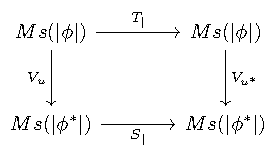
\includegraphics[width=0.45\textwidth]{./tikz-images/tikz-chap-d3.pdf}
\end{center}
% \begin{equation*}
% \begin{tikzcd}[column sep=large, row sep=large, scale=1.5]
% Ms(|\phi|) \arrow[r, "T_{|}"] \arrow[d, "V_u"'] & Ms(|\phi|) \arrow[d, "V_{u^{*}}"] \\
% Ms(|\phi^{*}|) \arrow[r, "S_{|}"'] & Ms(|\phi^{*}|)
% \end{tikzcd}
% \end{equation*}
%% --
In particular, $\sigma(S_{|}) = \sigma(T_{|})$.
Therefore we may deduce spectral properties of\/ $S_{|}$ from $T_{|}$ and vice versa.
More concrete applications of Lemma~\ref{lem:d3-1.2} will follow.
\end{remark}
%% --
\index{pseudo-resolvent|(}
We now investigate the fixed space 
%
\[
	\Fix{\RR} \coloneq \Fix{\lambda R(\lambda)} \quad (\lambda \in D) 
\]
%
of a pseudo-resolvent $\RR$ with values in the predual of a \WA-algebra $M$.
%% --
\begin{proposition}\label{prop:d3-1.4}
Let $\RR$ be a pseudo-resolvent on $D = \{\lambda \in \C \colon \Re(\lambda) > 0\}$ with values in the predual $M_{*}$ of a \WA-algebra $M$ and suppose $\RR$ to be identity preserving and of Schwarz type.
%% --
\begin{enumerate}[\upshape (i)]

\item\label{item:d3-1.4-i}
If\/ $\alpha \in \R$ and $\psi \in M_{*}$ such that $(\gamma - \im\alpha)R(\gamma)\psi = \psi$ for some $\gamma \in D$, then $\lambda R(\lambda)|\psi| = |\psi|$ and $\lambda R(\lambda)|\psi^{*}| = |\psi^{*}|$ for all $\lambda \in D$.

\item\label{item:d3-1.4-ii} 
$ \Fix{\RR} $ is invariant under the involution in $M_{*}$ and if\/ $\psi \in \Fix{\RR} $ is self-adjoint, then the positive part $\psi^{+}$ and the negative part $\psi^{-}$ of\/ $\psi$ are elements of\/ $ \Fix{\RR} $.
\end{enumerate}
\end{proposition}
%% -- 
\begin{proof}
If\/ $(\gamma - \im\alpha)R(\gamma)\psi = \psi$ then $(\lambda - \im\alpha)R(\lambda)\psi = \psi$ for all $\lambda \in D$ (use the resolvent equation to prove this).
In particular, 
%% --
\[
\mu R(\mu + \im\alpha)\psi = \psi \quad (\mu \in \R_{+}).
\]
For all $x \in M$ we obtain
%% --
\begin{align*}
|\psi(x)|^2 &= | \dualp{\mu R(\mu+\im\alpha)'x,\psi} |^2 \\
&\leq \|\psi\| \dualp{(\mu R(\mu+\im\alpha)'x)(\mu R(\mu+\im\alpha)'x)^{*},|\psi|}  \\
&\leq \|\psi\| \dualp{\mu R(\mu)'(xx^{*}),|\psi|}
\end{align*}
%% --
(see Corollary~\ref{cor:d1-2.2}).
Since
%% --
\begin{align*}
\|\psi\| &= \| |\psi| \| = |\psi|(\1) \\
&= \dualp{\mu R(\mu)'\1,\abs{\psi}} = \| \mu R(\mu)|\psi| \|,
\end{align*}
%% --
we obtain $\mu R(\mu)|\psi| = |\psi|$ by the uniqueness theorem \eqref{eq:star-uniqueness} on p.~\pageref{eq:star-uniqueness} for the absolute value.
Therefore $|\psi| \in \Fix{\RR} $.
Since
%% --
\[
0 \leq (\mu R(\mu)'x)(\mu R(\mu)'x)^{*} \leq \mu R(\mu)'xx^{*},
\]
%% --
the map $R(\mu)$ is positive.
Consequently 
%% --
\[
(\mu+\im\alpha)R(\mu)\psi^{*} = \psi^{*}
\]
%% --
from which 
%% --
\[
|\psi^{*}| \in \Fix{\RR} 
\]
%% 
follows.

If\/ $\phi \in \Fix{\RR} $ is self-adjoint with Jordan decomposition $\phi = \phi^{+} - \phi^{-}$, then for all $ R \in \RR $
%% --
\begin{align*}
\| \phi \| &= \| \phi^{+} \| + \| \phi^{-} \|  =
    \phi^{+}(\1) + \phi^{-}(\1) = \phi^{+}(R'\1) + \phi^{-}(R'\1) \\
    &= \dualp{\1, R(\phi^{+})}  + \dualp{\1, R(\phi^{-})}   =
    \| R(\phi^{+}) \| + \| R(\phi^{-}) \| .
\end{align*}
%% -- 
Then by \textcite[Theorem III.4.2.]{takesaki:1979} we obtain that $\phi^{+}$ and $\phi^{-}$ are in $ \Fix{\RR} $.
\end{proof}
%% --
\begin{corollary}\label{cor:d3-1.5}
Let $\TT$ be an identity preserving semigroup of Schwarz type on $M_{*}$ with generator $A$ and suppose $P\sigma(A) \cap \im\R \neq \emptyset$.
%% --
\begin{enumerate}[\upshape (i)]
\item
If\/ $\alpha \in \R$ and $\psi \in \operatorname{ker}(\im\alpha - A)$, then $|\psi|$ and $|\psi^{*}|$ are elements of\/ $\Fix{\TT} = \Kern{A}$.

\item 
$\Fix{\TT}$ is invariant under the involution of\/ $M_{*}$.
If\/ $\psi \in \Fix{\TT}$ is self-adjoint, then the positive part $\psi^{+}$ and the negative part $\psi^{-}$ of\/ $\psi$ are elements of\/ $\Fix{\TT}$.
\end{enumerate}
%% --
\end{corollary}
%% --
The proof follows immediately from Proposition~\ref{prop:d3-1.4} and the fact that 
%% --
\[ 
\Kern{A} = \Fix{\lambda R(\lambda,A)}
\]
%% --
for all $\lambda \in \C$ with $\Re(\lambda) > 0$.

If\/ $\TT$ is the semigroup of translations on $L^1(\R)$ and $A'$ the generator 
of the adjoint weak*-semigroup, then $P\sigma(A) \cap \im\R = \emptyset$, while $P{\sigma}(A') \cap \im\R = \im\R$.
For that reason we cannot expect a simple connection between these two sets.
But as we shall see below, if a semigroup on the predual of a \WA-algebra has sufficiently many invariant states, then the point spectra contained in $\im\R$ of\/ $A$ and $A'$  are identical.

Helpful for these investigations will be the next lemma.
%% --
\begin{lemma}\label{lem:d3-1.6}
Let $\RR$ be a pseudo-resolvent on $D = \{\lambda \in \C \colon \Re(\lambda) > 0\}$ with values in a Banach space $E$ such that $\|R(\mu + \im\alpha)\| \leq 1$ for all $(\mu,\alpha) \in \R_{+} \times \R$.
Then
%% --
\[
\dim \Fix{\lambda R(\lambda + \im\alpha)} \leq \dim \Fix{\lambda R(\lambda + \im\alpha)'} 
\]
%% --
for all $\lambda \in D$.
\end{lemma}
%% --
\begin{proof}
Let $(\mu,\alpha) \in \R_{+} \times \R$ and $S \coloneq \mu R(\mu + \im\alpha)$.
Since $S$ is a contraction, its adjoint $S'$ maps the dual unit ball $E'_{1}$ into itself.

Let $\mathfrak{U}$ be a free ultrafilter on $ \left[1,\infty \right)$ which converges to $1$.
Since $E'_{1}$ is $\sigma(E',E)$-compact, 
%% --
\[
\psi_{0} \coloneq \lim_{\mathfrak{U}}(\lambda - 1)R(\lambda,S)'\psi
\]
%% --
exists for each $\psi \in E'_{1}$.
Since $S'$ is $\sigma(E',E)$-continuous and since $S'R(\lambda,S)' = \lambda R(\lambda,S')-\Id$ we conclude $\psi_{0} \in \Fix  {S'}$.

Take now $0 \neq x_{0} \in \Fix{S}$ and choose $\psi \in E'_{1}$ such that $\psi(x_{0})$ is different from zero.
From the considerations above it follows
%% --
\[ 
\psi_{0}(x_{0}) = \lim_{\mathfrak{U}}(\lambda - 1)\psi(R(\lambda,S)x_{0}) = \psi(x_{0}) \neq 0 ,
\]
%% --
hence $0 \neq \psi_{0} \in \Fix{S'}$.
Therefore $\Fix{S'}$ separates the points of\/ $\Fix{S}$.
From this it follows that
%% --
\[
	\dim \Fix{S} \leq \dim \Fix{S'} .
\]
%% --
Since $\RR$ and $\RR'$ are pseudo-resolvents, the assertion is proved.
\end{proof}
%% --
\begin{corollary}\label{cor:d3-1.7}
Let $\TT$ be a semigroup of contractions on a Banach space $E$ with generator $A$.
Then
%% --
\[
\dim \Kern{\im\alpha - A} \leq \dim \Kern{\im\alpha - A'}
\]
%% --
for all $\alpha \in \R$.
\end{corollary}
%% --
%% -- d3-8
This follows from Lemma~\ref{lem:d3-1.6} because $\Fix{\lambda R(\lambda+\im\alpha)} = \Kern{\im\alpha-A}$.
%% --
\begin{proposition}\label{prop:d3-1.8}
Let $\TT$ be an identity preserving semigroup of Schwarz type with generator $A$ on the predual of a \WA-algebra and suppose that there exists a faithful family $\Psi$ of\/ $\TT$-invariant states.
Then for all $\alpha \in \R$ we have
%% --
\[
\dim \Kern{\im\alpha - A} = \dim \Kern{\im\alpha - A'}
\]
%% --
and
%% --
\[
P\sigma(A) \cap \im\R = P{\sigma}(A') \cap \im\R .
\]
%% --
\end{proposition}
%% --
\begin{proof}
The inequality $\dim \Kern{\im\alpha - A} \leq \dim \Kern{\im\alpha - A'}$ follows from Corollary~\ref{cor:d3-1.7}.

Let $D = \{\lambda \in \C \colon \Re(\lambda) > 0\}$ and $\RR$ the pseudo-resolvent induced by $R(\lambda,A)$ on $D$.
Then $\RR$ is identity preserving and of Schwarz type.
Take $\im\alpha \in P\sigma(A)$ ($\alpha \in \R$) and choose $0 < \mu \in \R$.

If\/ $\psi_{\alpha} \in M_{*}$ is of norm one with polar decomposition $\psi_{\alpha} = u_{\alpha}|\psi_{\alpha}|$ such that $\psi_{\alpha} = (\mu - \im\alpha)R(\mu)\psi_{\alpha}$ then $\mu R(\mu)|\psi_{\alpha}| = |\psi_{\alpha}|$ (Proposition~\ref{prop:d3-1.4}\,\ref{item:d3-1.4-i}).

Since
%% --
\[
\mu R(\mu)'(\1 - s(|\psi_{\alpha}|)) 
    \leq \1 - s(|\psi_{\alpha}|) ,
\]
%% --
we obtain $\mu R(\mu)'s(|\psi_{\alpha}|) = s(|\psi_{\alpha}|)$ by the faithfulness of\/ $\Psi$.

Hence the maps 
%% --
\[
S \coloneq (\mu - \im\alpha)R(\mu)'  
\quad \text{and} \quad 
T \coloneq \mu R(\mu)'
\]
%% --
fulfill the assumptions of Lemma~\ref{lem:d3-1.2}\,\ref{item:d3-1.2-ii}.
Therefore $Su_{\alpha}^{*} = u_{\alpha}^{*}$ or 
%% --
\[
(\mu-\im\alpha)R(\mu)'u_{\alpha}^{*} = u_{\alpha}^{*}
\]
%% --
which implies $u_{\alpha}^{*} \in D(A')$ and 
%% --
\[
A'u_{\alpha}^{*} = \im\alpha u_{\alpha}^{*}.
\]
%% --

If\/ $\im\alpha \in P{\sigma}(A')$, $\alpha \in \R$, choose $0 \neq v_{\alpha}$ such that
%% --
\[
v_{\alpha} = (\mu - \im\alpha)R(\mu)'v_{\alpha} \quad (\mu \in \R_{+})
\]
%% --
and $\psi \in \Psi$ such that $\psi(v_{\alpha}v_{\alpha}^{*}) \neq 0$.

Since
%% --
\[
0 \leq v_{\alpha}v_{\alpha}^{*} = ((\mu - \im\alpha)R(\mu)'v_{\alpha})((\mu - \im\alpha)R(\mu)'v_{\alpha})^{*} \leq \mu R(\mu)'(v_{\alpha}v_{\alpha}^{*}) ,
\]
%% --
we obtain $\mu R(\mu)'(v_{\alpha}v_{\alpha}^{*}) = v_{\alpha}v_{\alpha}^{*}$ because $\Psi$ is faithful.

Hence from Lemma~\ref{lem:d3-1.2}\,\ref{item:d3-1.2-i} it follows that
%% --
\[
\mu R(\mu)'(xv_{\alpha}^{*}) = ((\mu - \im\alpha)R(\mu)'x)v_{\alpha}^{*}
\]
%% --
for all $x \in M$.

Let $\psi_{\alpha}$ be the normal linear functional $(x \mapsto \psi(xv_{\alpha}^{*}))$ on $M$ and note that \mbox{$\psi_{\alpha}(v_{\alpha}) \neq 0$}.
Then
%% --
\begin{align*}
\langle x, (\mu - \im\alpha)R(\mu)\psi_{\alpha} \rangle &= \langle ((\mu - \im\alpha)R(\mu)'x)v_{\alpha}^{*},\psi \rangle \\
&= \langle \mu R(\mu)'(xv_{\alpha}^{*}),\psi \rangle = \psi(xv_{\alpha}^{*}) = \psi_{\alpha}(x)
\end{align*}
%% --
for all $x \in M$.
Consequently $\im\alpha \in P\sigma(A)$ and
%% --
\[
\dim \Kern{\im\alpha - A'} \leq \dim \Kern{\im\alpha - A}
\]
%% --
which proves the assertion.
\end{proof}
\index{pseudo-resolvent|)}

%% --
\begin{remark}\label{rem:d3-1.9}
From the above proof we obtain the following: If 
\mbox{$0 \neq \psi_{\alpha} \in \Kern{\im\alpha - A}$} for $ \alpha \in \R $ with polar decomposition 
$\psi_{\alpha} = u_{\alpha}|\psi_{\alpha}|$ ($\alpha \in \R$), 
then $A'u_{\alpha}^{*} = \im\alpha u_{\alpha}^{*}$.

Conversely, if\/ $0 \neq v_{\alpha} \in \Kern{\im\alpha - A'}$, then there exists $\psi \in \Psi$ such that 
\mbox{$\psi(v_{\alpha}v_{\alpha}^{*}) \neq 0$} and the normal linear form
%% --
\[
\psi_{\alpha} \coloneq (x \mapsto \psi(xv_{\alpha}^{*}))
\]
%% --
is an eigenvector of\/ $A$ pertaining to the eigenvalue $\im\alpha$.
\end{remark}
%% --
If\/ $\TT$ is a $C_{0}$-semigroup of Markov operators on a commutative \CA-algebra with generator $A$, it has been shown in Part-II, Chapter~\ref{chap:b3},  that the boundary spectrum $\sigma(A) \cap \im\R$ of its generator is additively cyclic.
This is no longer true in the noncommutative case.
%% --
\begin{example*}\label{ex:d3-1.10}
For $0 \neq \lambda \in \im\R$ and $t \in \R$ let
%% --
\[
u_{t} \coloneq \begin{pmatrix} 1 & 0 \\ 
0 & \eu^{\lambda t} \end{pmatrix} 
\in M_{2}(\C) .
\]
%% --
The semigroup of *-automorphisms $(x \mapsto u_{t}xu_{t}^{*})$ on $M_{2}(\C)$ is identity preserving and of Schwarz type, but the spectrum of its generator is $\{0, \lambda, \overline{\lambda}\}$ hence is not additively cyclic.
\end{example*}
%% --
It turns out that, in order to obtain a noncommutative analogue of the Perron-Frobenius theorems, one has to consider semigroups which are irreducible.

Recall that a semigroup $\SG$ of positive operators on an ordered Banach space $(E,E_{+})$ is called \emph{irreducible} if no closed face of\/ $E_{+}$, different from $\{0\}$ and $E_{+}$, is invariant under $\SG$.
%Here a face $F$ in $E$ is a subcone of\/ $E_{+}$ such that the conditions $0 \leq x \leq y$, $x \in E$, $y \in F$ imply $x \in F$ (compare Definitions 3.1 in Part-II, Chapter~\ref{chap:b3} and Part-3, Chapter~\ref{chap:c3}).
In the context of \WA-algebras $M$ we call a semigroup $\SG$ of positive maps on $M$ \emph{weak*-irreducible} if no non-trivial $\sigma(M,M_{*})$-closed face of\/ $M_{+}$ is $\SG$-invariant.

Since the norm closed faces of\/ $M_{*}$ and the $\sigma(M,M_{*})$-closed faces of\/ $M$ are related by formation of polars with respect to the dual system $\langle M,M_{*} \rangle$ (see \textcite[Theorem 3.6.11 and Theorem 3.10.7.]{pedersen:1979}) a semigroup $\SG$ is (norm) irreducible on $M_{*}$ if and only if its adjoint semigroup is weak*-irreducible.
%% --
\index{irreducible semigroup}
%% --
\begin{theorem}\label{thm:d3-1.11}
Let $\TT$ be an irreducible, identity preserving semigroup of Schwarz type with generator $A$ on the predual of a \WA-algebra and suppose $P\sigma(A) \cap \im\R \neq \emptyset$.
%% --
\begin{enumerate}[\upshape (i)]
\item 
The fixed space of\/ $\TT$ is one-dimensional and spanned by a faithful normal state.

\item 
$P\sigma(A) \cap \im\R$ is an additive subgroup of\/ $\im\R$,
%% --
\[
\sigma(A) = \sigma(A) + (P\sigma(A) \cap \im\R)
\]
%% --
and every eigenvalue in $\im\R$ is simple.

\item 
The fixed space of the adjoint weak*-semigroup $\TT'$ is one-dimensional.

\item 
$P{\sigma}(A') \cap \im\R = P\sigma(A) \cap \im\R$ for the generator $A'$ of the adjoint semigroup, and every $\gamma \in P{\sigma}(A') \cap \im\R$ is simple.
\end{enumerate}
\end{theorem}
%% --
\begin{proof}
Since $P\sigma(A) \cap \im\R \neq \emptyset$, there exists $\psi \in \Fix{\TT}_{+}$ of norm one (Corollary~\ref{cor:d3-1.5}).
If\/ $F \coloneq \{x \in M_{+} \colon \psi(x) = 0\}$, then $F$ is a $\sigma(M,M_{*})$-closed, $\TT'$-invariant face in $M$, hence $F = \{0\}$.
Therefore every $0 \neq \psi \in \Fix{\TT}_{+}$ is faithful.

Let $\psi_{1}$, $\psi_{2} \in \Fix{\TT}_{+}$ be states such that $f \coloneq \psi_{1} - \psi_{2}$ is different from zero. 
If\/ $f = f^{+} - f^{-}$ is the Jordan decomposition of\/ $f$, then $f^{+}$ and $f^{-}$ are elements of\/ $\Fix{\TT}$, whence faithful.
Since the support projections of these two normal linear functionals are orthogonal, we obtain $f^{+} = 0$ or $f^{-} = 0$ which implies $\psi_{1} \leq \psi_{2}$ or $\psi_{2} \leq \psi_{1}$.
Consequently $\psi_{2} = \psi_{1}$.

Since $\Fix{\TT}$ is positively generated (Corollary~\ref{cor:d3-1.5}), 
%% --
\[
\Fix{\TT} = \{ \lambda \phi \colon \lambda \in \C \} \eqcolon \C.\phi
\]
%% --
for some faithful normal state $\phi$.

Let $\mu \in \R_{+}$ and $\alpha \in \R$ such that $\im\alpha \in P\sigma(A)$.
If\/ $\psi_{\alpha} = u_{\alpha}|\psi_{\alpha}|$ is a normalized eigenvector of\/ $A$ pertaining to $\im\alpha$, then $\phi = |\psi_{\alpha}| = |\psi_{\alpha}^{*}|$, hence 
%
\[
	u_{\alpha}u_{\alpha}^{*} = u_{\alpha}^{*}u_{\alpha} = s(\phi) = \1
\]
%
(Corollary~\ref{cor:d3-1.5} and the above considerations).

Since
%% --
\[
(\mu - \im\alpha)R(\mu,A)\psi_{\alpha} = \psi_{\alpha}
\]
%% --
and
%% --
\[
\mu R(\mu,A)|\psi_{\alpha}| = |\psi_{\alpha}| ,
\]
%% --
we obtain by Lemma~\ref{lem:d3-1.2}\,\ref{item:d3-1.2-ii} that
%% --
\[
\mu R(\mu,A) = V_{\alpha} \circ \mu R(\mu+\im\alpha,A) \circ V_{\alpha}^{-1} \tag{1}
\]
%% --
where $V_{\alpha}$ is the map $(x \mapsto xu_{\alpha})$ on $M$.

Similarly, for $\im\beta \in P\sigma(A)$ we find $V_{\beta}$ such that $\1 = u_{\beta}u_{\beta}^{*} = u_{\beta}^{*}u_{\beta}$ and
%% --
\[
\mu R(\mu,A) = V_{\beta} \circ \mu R(\mu+ \iu \beta,A) \circ V_{\beta}^{-1} \tag{2} 
\]
%% --
Hence
%% --
\[
\mu R(\mu,A) = V_{\alpha\beta} \circ \mu R(\mu+ \iu (\alpha+\beta),A) \circ V_{\alpha\beta}^{-1} \tag{3}
\]
%% --
where $V_{\alpha\beta} \coloneq V_{\alpha} \circ V_{\beta}$.

Since $u_{\alpha}$ is unitary in $M$, it follows from (1) that $\im\alpha$ is an eigenvalue which is simple because $\Fix{\TT} = \Fix{\mu R(\mu,A)}$ is one-dimensional.

From (3) it follows that $\iu(\alpha+\beta) \in P\sigma(A)$ since $0 \in P\sigma(A)$ and $V_{\alpha\beta}$ is bijective.
From the identity (1) we conclude that $\sigma(R(\mu,A)) = \sigma(R(\mu+\im\alpha,A))$, which proves
%% --
\[
\sigma(A) + (P\sigma(A) \cap \im\R) \subseteq \sigma(A).
\]
%% --
The other inclusion is trivial since $0 \in P\sigma(A)$.
\end{proof}
%% --
\begin{remarks}\label{rem:d3-1.12}
%% --
\begin{enumerate}[\upshape (i), wide, labelindent=.25em]

\item 
Let $\phi$ be the normal state on $M$ such that 
$\Fix{\TT} = \C.\phi$ and let $H \coloneq P\sigma(A) \cap \im\R$.
From the proof of Theorem~\ref{thm:d3-1.11} it follows that there exists a family $\{u_{\eta} \colon \eta \in H\}$ of unitaries in $M$ such that $A'u_{\eta} = -\eta u_{\eta}$ and $A(u_{\eta}\phi) = \eta(u_{\eta}\phi)$ for all $\eta \in H$.

\item 
If the group $H$ is generated by a single element, \ie $H = \im\gamma\Z$ for some $\gamma \in \R$, then 
$\{u_{\gamma}^{k} \colon k \in \Z\}$ 
is a complete family of eigenvectors pertaining to the eigenvalues in $H$, where $u_{\gamma} \in M$ is unitary such that $A'u_{\gamma} = \im\gamma u_{\gamma}$.

\end{enumerate}
\end{remarks}
%% --
\begin{proposition}\label{prop:d3-1.13}
Suppose that $\TT$ and $M$ satisfy the assumptions of Theorem~\ref{thm:d3-1.11}, and let $N_{*}$ be the closed linear subspace of\/ $M_{*}$ generated by the eigenvectors of\/ $A$ pertaining to the eigenvalues in $\im\R$.
Denote by $\TT_{0}$ the restriction of\/ $\TT$ to $N_{*}$.
Then
\begin{enumerate}[\upshape (i)]
 
\item 
$G \coloneq \overline{\TT_{0}} \subseteq \mathcal{L}_{s}(N_{*})$ is a compact, Abelian group in the strong operator topology.

\item 
$\Id_{| N_{{*}}} \in \overline{\{T_{0}(t) \colon t>s\}} \subseteq \mathcal{L}_{s}(N_{*})$ for all $0<s \in \R$.
\end{enumerate}
\end{proposition}
%% --
\begin{proof}
For $\eta \in \Omega \coloneq P\sigma(A) \cap \im\R$ let
%% --
\[
U(\eta) \coloneq \{\psi \in D(A) \colon A\psi = \eta\psi\}
\]
%% --
and $U \coloneq \bigcup_{\eta \in \Omega} U(\eta)$. 
Then $\closure{U} = N_{*}$, where $\closure{U}$ denotes the closure of $U$.

For each $\psi \in U$ there exists $\eta \in \Omega$ such that
%% --
\[
\{T_{0}(t)\psi \colon t \in \R_{+}\} = \{\eu^{\eta t}\psi \colon t \in \R_{+}\} .
\]
%% --
Consequently this set is relatively compact in $\mathcal{L}_{s}(N_{*})$.
From \textcite[III.4.5]{schaefer:1966} we obtain that $G$ is compact in the strong operator topology.

Next choose $\psi_{1}, \dots, \psi_{n} \in U$, $0 < s \in \R$ and $\delta > 0$.
Since 
%% --
\[
T_{0}(t)\psi_{i} = \eu^{\eta_{i}t}\psi_{i} 
\quad (1 \leq i \leq n)
\]
%% --
for some $\eta_{i} \in \Omega$, it follows from a theorem of Kronecker (see \textcite[Satz 6.1, p.~77]{jacobs:1972}) that there exists $s < t$ such that
%% --
\[
|(1,1, \dots, 1) - (\eu^{\eta_{1}t}, \eu^{\eta_{2}t}, \dots, \eu^{\eta_{n}t})| < \delta ,
\]
%% --
hence
%% --
\[
\sup\{\|\psi_{i} - T_{0}(t)\psi_{i}\| \colon 1 \leq i \leq n\} < \delta
\]
%% --
or 
\[
\Id_{|N_{*}} \in \overline{\{T_{0}(t) \colon t>s\}} \subseteq \mathcal{L}_{s}(N_{*}).
\]
%% --

Finally we prove the group property of\/ $G$.
Let $\mathfrak{U}$ be an ultrafilter on $\R$ such that $\lim_{\mathfrak{U}}T_{0}(t) = \Id$ in the strong operator topology.
For positive $s \in \R$ let 
%
\[
	S \coloneq \lim_{\mathfrak{U}}T_{0}(t-s) .
\]
%
Then 
%
\[
	S \cdot T_{0}(s) = T_{0}(s)S = \Id
\]
%
and $T_{0}(s)^{-1}$ exists in $G$ for all $s \in \R_{+}$.
From this it follows that $G$ is a group.
\end{proof}
%% --
\begin{remark}\label{rem:d3-1.14}
\begin{enumerate}[\upshape (i), wide, labelindent=.25em]
\item Let $\kappa \colon \R \to G$ be given by
%% --
\[
\kappa(t) = \begin{cases}
T_{0}(t) & \text{if } 0 \leq t , \\
T_{0}(t)^{-1} & \text{if } t \leq 0.
\end{cases}
\]
%% --
Then $\kappa$ is a continuous homomorphism with dense range, \ie $(G,\kappa)$ is solenoidal (see \textcite{hewittross:1963}).

\item 
The compact group $G$ and the discrete group $P\sigma(A) \cap \im\R$ are dual as locally compact Abelian groups.

\item 
Let $(G,\kappa)$ be a solenoidal compact group and let $N_{*} = L^{1}(G)$.
Then the induced lattice semigroup $\TT = (\kappa(t))_{t \geq 0}$ fulfils the assertions of Theorem~\ref{thm:d3-1.11}.
For example, if\/ $G$ is the dual of\/ $\R_{d}$, then $P\sigma(A) \cap \im\R = \im\R$.
Since the fixed space of\/ $\kappa(t)$ is given by
%% --
\[
	\Fix{\kappa(t)} = 
    \overline{ \left(\bigcup_{k \in \Z} \Kern{2\pi \iu k /t - A} \right) } ,
\]
%% --
however no $T(t) \in \TT$ is irreducible.

\item 
If\/ $\TT$ is the irreducible semigroup of Schwarz type on the predual of\/ $\BH$ given in \textcite{evans:1977}, then $P\sigma(A) \cap \im\R = \emptyset$.
\end{enumerate}
\end{remark}
%% --
\section{Spectral Properties of Uniformly Ergodic Semigroups}\label{sec:d3-2}
%% --
The aim of this section is the study of spectral properties of semigroups which are uniformly ergodic, identity preserving and of Schwarz type.
For the basic theory of uniformly ergodic semigroups on Banach spaces we refer to \textcite{dunfordschwartz:1958}.

Our first result yields an estimate for the dimension of the eigenspaces pertaining to eigenvalues of a pseudo-resolvent.
% --
\begin{proposition}\label{prop:d3-2.1}
Let $\RR$ be an identity preserving pseudo-resolvent of Schwarz type on $D = \{\lambda \in \C \colon \Re(\lambda) > 0\}$ with values in the predual of a \WA-algebra $M$. 
If\/ $\Fix{\lambda R(\lambda)}$ is finite dimensional for some $\lambda \in D$, then
%% --
\[
\dim \Fix{\left( \gamma - \im\alpha \right)R(\gamma)} \leq \dim \Fix{\lambda R(\lambda)}
\]
%% --
for all $\gamma \in D$ and $\alpha \in \R$.
\end{proposition}
%% --
\begin{proof}
By Remark~\ref{rem:d4-3.2}, we may assume without loss of generality that there exists a faithful family of\/ $\RR$-invariant normal states on $M$.
In particular the fixed space $N$ of the adjoint pseudo-resolvent $\RR'$ is a \WA-subalgebra of\/ $M$ with $\1 \in N$ (by Lemma~\ref{lem:d3-1.1}\,\ref{item:d3-1.1-ii}).
Since $N$ is finite dimensional, there exist a natural number $n$ and a set $P \coloneq \{p_{1}, \ldots, p_{n}\}$ of minimal, mutually orthogonal projections in $N$ such that $\sum_{k=1}^{n} p_{k} = \1$.
These projections are also mutually orthogonal in $M$ with sum $\1$.

Let $R_{j}$ be the $\sigma(M,M_{*})$-closed right ideal $p_{j}M$ and $L_{j}$ the closed left invariant subspace $M_{*}p_{j}$ for $(1 \leq j \leq n)$.
Since the map $\mu R(\mu)'$, $\mu \in \R_{+}$ is an identity preserving Schwarz map, we obtain from Lemma~\ref{lem:d3-1.1}\,\ref{item:d3-1.1-ii} that for all $x \in N$ and $y \in M$,
%% --
\[
	\mu R(\mu)'(xy) = x(\mu R(\mu)'y) .
\]
%% --
In particular, $R_{j}$, \resp $L_{j}$ are invariant under $\RR'$, respectively, $\RR$.
Furthermore, if\/ $\psi \in L_{j}$ with polar decomposition $\psi = u|\psi|$, then $u^{*}u \leq s(|\psi|) \leq p_{j}$.
Consequently, $|\psi| \in L_{j}$.

Let now $\alpha \in \R$ and suppose that there exists $\psi_{\alpha} \in L_{j}$ of norm $ 1 $, $\psi_{\alpha} = u_{\alpha}|\psi_{\alpha}|$, such that
%% --
\[
	\psi_{\alpha} \in \Fix  {(\lambda - \im\alpha)R(\lambda)} , \lambda \in D .
\]
%% --
Since $\lambda R(\lambda)|\psi_{\alpha}| = |\psi_{\alpha}|$ (Proposition~\ref{prop:d3-1.4}), we obtain
%% --
\[
	\mu R(\mu)'(\1-s(|\psi_{\alpha}|)) \leq \1-s(|\psi_{\alpha}|) , \mu \in \R_{+} .
\]
%% --
From the existence of a faithful family of\/ $\RR$-invariant normal states and since $\RR'$ is identity preserving, it follows that
%% --
\[
	\mu R(\mu)'s(|\psi_{\alpha}|) = s(|\psi_{\alpha}|) .
\]
%% --
Thus $s(|\psi_{\alpha}|) \leq p_{j}$ and even $s(|\psi_{\alpha}|) = p_{j}$ by the minimality property of\/ $p_{j}$.

On the other hand, $\psi_{\alpha}^{*} \in \Fix  {(\lambda + \im\alpha)R(\lambda)}$.
As above we obtain
%% --
\[
\mu R(\mu)'s(|\psi_{\alpha}^{*}|) = s(|\psi_{\alpha}^{*}|) .
\]
%% --
Consequently, the closed left ideals $Ms(|\psi_{\alpha}^{*}|)$ and $Ms(|\psi_{\alpha}|)$ are $\RR'$-invariant.

Next fix $\mu \in \R_{+}$, let $S \coloneq (\mu - \im\alpha)R(\mu)'$ and $T = \mu R(\mu)'$.
Then 
%
\[
	(Sx)(Sx)^{*} \leq T(xx^{*}), \,
	S_{*}(\psi_{\alpha}^{*}) = \psi_{\alpha}^{*}, \,
	T_{*}(|\psi_{\alpha}^{*}|) = |\psi_{\alpha}^{*}|, 
\]
%
and $T$ is an identity preserving Schwarz map.
Since $s(|\psi_{\alpha}^{*}|)M$ is $T$-invariant, the assumptions of Lemma~\ref{lem:d3-1.2} are fulfilled and we obtain for every $x \in M$
%% --
\[
	S(x)u_{\alpha}^{*} = T(xu_{\alpha}^{*}) .
\]
%% --
The closed left ideal $Mp_{j}$ is $S$-invariant, therefore it follows
%% --
\[
S(x) = T(xu_{\alpha}^{*})u_{\alpha} \, , \, x \in Mp_{j}
\]
%% --
(see Remark~\ref{rem:d3-1.3}).
Since $u_{\alpha}$ does not depend on $\mu \in \R_{+}$, we obtain for all $\mu \in \R_{+}$
%% --
\[
\mu R(\mu+\im\alpha)'x = \mu R(\mu)'(xu_{\alpha}^{*})u_{\alpha}.
\]
%% --
Consequently, the holomorphic functions 
%
\[
	(\mu \mapsto \mu R(\mu)'(x u_{\alpha}^{*})u_{\alpha})
	\quad \text{and} \quad
	(\mu \mapsto \mu R(\mu+\im\alpha)'x)
\]
%
coincide on $\R_{+}$ from which we conclude
%% --
\[
\lambda R(\lambda+\im\alpha)'x = \lambda R(\lambda)'(xu_{\alpha}^{*})u_{\alpha}
\]
%% --
for every $\lambda \in D$ and all $x \in Mp_{j}$.

Since the map $(y \mapsto y u_{\alpha})$ is a continuous bijection from $M(u_{\alpha}u_{\alpha}^{*})$ onto $Mp_{j}$ with inverse $(y \mapsto y u_{\alpha}^{*})$, we can deduce that
%% --
\begin{align*}
\dim \Fix  {(\lambda-\im\alpha)R(\lambda)'|Mp_{j}} 
	&= \dim \Fix{\lambda R(\lambda)'|M(u_{\alpha}u_{\alpha}^{*})}  \\
 	&\leq \dim \Fix  {\RR'} .
\end{align*}
%% --
Since 
%
\[
	\bigoplus_{j=1}^{n} Mp_{j} = M 
	\quad \text{and} \quad 
	\bigoplus_{j=1}^{n} L_{j} = M_{*},
\]
%
we obtain
%% --
\begin{align*}
\dim \Fix  {(\lambda - \im\alpha)R(\lambda)'} &= \dim \Fix{\lambda R(\lambda)'} \\
		&= \dim \Fix  {\lambda R(\lambda)} ,
\end{align*}
%% --
% -- d3-16
%% --
and the assertion follows from Lemma~\ref{lem:d3-1.6}.
\end{proof}
%% --
Before going on let us recall the basic facts of the \emph{ultrapower} $\widehat{E}$ of a Banach space $E$ with respect to some free ultrafilter $\mathfrak{U}$ on $\N $ (compare Part-I, Section~\ref{subsec:a1-3.7}).
If\/ $\ell^{\infty}(E)$ is the Banach space of all bounded functions on $\N $ with values in $E$, then
%% --
\[
c_{\mathfrak{U}}(E) \coloneq \{(x_{n}) \in \ell^{\infty}(E) \colon \lim_{\mathfrak{U}}\|x_{n}\| = 0\}
\]
%% --
is a closed subspace of\/ $\ell^{\infty}(E)$ and equal to the kernel of the seminorm
%% --
\[
\|(x_{n})\| \coloneq \lim_{\mathfrak{U}}\|x_{n}\| \, , \, (x_{n}) \in \ell^{\infty}(E).
\]
%% --
By the \emph{ultrapower} $\widehat{E}$ we understand the quotient space $\ell^{\infty}(E)/c_{\mathfrak{U}}(E)$ with norm
%% --
\[
\|\hat{x}\| = \lim_{\mathfrak{U}}\|x_{n}\| \, , \, (x_{n}) \in \hat{x} \in \widehat{E}.
\]
%% --
Moreover, for a bounded linear operator $T \in \LE$, we denote by $\widehat{T}$ the well defined operator $\widehat{T}\hat{x} \coloneq (Tx_{n}) + c_{\mathfrak{U}}(E)$, $(x_{n}) \in \hat{x}$.

It is clear by virtue of\/ $(x \mapsto (x, x, \dots) + c_{\mathfrak{U}}(E))$ that each $x \in E$ defines an element $\hat{x} \in \widehat{E}$.
This isometric embedding as well as the operator map $(T \mapsto \widehat{T})$ are called canonical.
\index{pseudo-resolvent|(}
In particular, if\/ $\RR \colon (D \to \LE)$ is a pseudo-resolvent, then
%% --
\[
\widehat{\RR} \coloneq (\lambda \mapsto R(\lambda)^{\wedge}) \colon D \to \mathcal{L}(\widehat{E})
\]
%% --
is a pseudo-resolvent, too.
Recall that the approximative point spectrum $A{\sigma}(T)$ is equal to the point spectrum $P{\sigma}(\widehat{T})$ (see, \eg \textcite[Chapter V, §1]{schaefer:1974}).

This construction gives us the possibility to characterize uniformly ergodic semigroups with finite dimensional fixed space.
%% --
\index{resolvent!pole|(}
\begin{lemma}\label{lem:d3-2.2}
Let $\RR$ be a pseudo-resolvent on $D = \{\lambda \in \C \colon \Re(\lambda) > 0\}$ such that $\|\mu R(\mu+\im\alpha)\| \leq 1$ for all $(\mu,\alpha) \in \R_{+} \times \R$ and suppose
%% --
\[
0 < \dim \Fix  {(\lambda-\im\alpha)\widehat{R}(\lambda)} < \infty \quad \text{for some} \quad \lambda \in D \, , \, \alpha \in \R .
\]
%% --
For the canonical extension $\widehat{R}$ on some ultrapower $\widehat{E}$, the following assertions hold.
%% --
\begin{enumerate}[\upshape (i)]
\item\label{d3-2.2-i}
$(\lambda - \im\alpha)^{-1}$ is a pole of the resolvent $R(.,R(\lambda))$ for all $\lambda \in D$.

\item\label{d3-2.2-ii}
$\dim \Fix  {(\lambda-\im\alpha)R(\lambda)} 
	= \dim \Fix{(\lambda-\im\alpha)\widehat{R}(\lambda)}$ for all $\lambda \in D$.

\item\label{d3-2.2-iii}
$\im\alpha$ is a pole of the pseudo-resolvent $\RR$ and the residue of\/ $\RR$ and $R(.,R(\lambda))$ in $\im\alpha$ respectively $(\lambda - \im\alpha)^{-1}$ are identical.

\end{enumerate}
\end{lemma}
%% --
\begin{proof}
Take a normalized sequence $(x_{n})$ in $E$ with
%% --
\[
\lim_{n}\|(\lambda - \im\alpha)R(\lambda)x_{n} - x_{n}\| = 0 .
\]
%% --
Since the fixed space of {$(\lambda-\im\alpha)\widehat{R}(\lambda)$} is non trivial such a sequence exists.
Suppose $\{ x_{n} \colon n\in\N \}$ is not relatively compact.
Then we may assume that there exists $\delta > 0$ such that
%% --
\[
	\|x_{n} - x_{m}\| > \delta \quad \text{for} \quad n \neq m .
\]
%% --
Take $k \in \N $ and let $\hat{x}_{k}$ be the image of\/ $(x_{n+k})$ in $\widehat{E}$.
Since
%% --
\[
	\lim_{n}\|(\lambda - \im\alpha)R(\lambda)x_{n+k} - x_{n+k}\| = 0 ,
\]
%% --
the so defined $\hat{x}_{k}$'s belong to $\Fix{(\lambda - \im\alpha)\widehat{R}(\lambda)}$.
Since this space is finite dimensional there exist $j < \ell$,  such that
%% --
\[
	\|\hat{x}_{j} - \hat{x}_{\ell}\| \leq \frac{\delta}{2} .
\]
%% --
From the definition of the norm in $\widehat{E}$ it follows that there are natural numbers $n < m$ such that
%% --
\[
\|x_{n} - x_{m}\| \leq \frac{\delta}{2} ,
\]
%% --
leading to a contradiction.

Therefore every approximate eigenvector of\/ $(\lambda - \im\alpha)R(\lambda)$ pertaining to $\alpha$ is relatively compact.
In particular, it has a convergent subsequence from which it follows that the fixed space of\/ $(\lambda - \im\alpha)R(\lambda)$ is non trivial.

Obviously
%% --
\[
\dim \Fix{(\lambda - \im\alpha)R(\lambda)} \leq \dim \Fix{(\lambda - \im\alpha)\widehat{R}(\lambda)} .
\]
%% --
%% -- d3-18
%% --
If the last inequality is strict, then there exists $\gamma > 0$ and a normalized 
$\hat{x} \in \Fix  {(\lambda - \im\alpha)\widehat{R}(\lambda)}$ such that
%% --
\[
\gamma \leq \|\hat{y} - \hat{x}\|
\]
%% --
for all $y \in \Fix  {(\lambda - \im\alpha)R(\lambda)}$.

Take a normalized sequence $(x_{n}) \in \hat{x}$.
Then $(x_{n})$ has a convergent subsequence, whence we may assume that $\lim_{n} x_{n} = z$ exists in $E$.
Thus $0 \neq z \in \Fix{(\lambda - \im\alpha)R(\lambda)}$.
From this we obtain the contradiction
%% --
\[
 0 \leq \gamma \leq \|\hat{z} - \hat{x}\| = \lim_{n} \|z - x_{n}\| = 0 .
\]
%% --
Consequently,
%% --
\[
\dim \Fix{(\lambda - \im\alpha)R(\lambda)} = \dim \Fix{(\lambda - \im\alpha)\widehat{R}(\lambda)}.
\]
%% --
Let $\{x_{1},\dots,x_{n}\}$ be a base of 
$\Fix{(\lambda - \im\alpha)R(\lambda)}$ and choose $\{\phi_{1},\dots,\phi_{n}\}$ in 
$\Fix{(\lambda - \im\alpha)R(\lambda)'}$ such that $\phi_{k}(x_{j}) = \delta_{k,j}$ 
(Lemma~\ref{lem:d3-1.6}).

Then
%% --
\[
E = \Fix{(\lambda - \im\alpha)R(\lambda)} \oplus \bigcap_{j=1}^{n} \Kern{\phi_{j}},
\]
%% --
where both subspaces on the right are 
$(\lambda - \im\alpha)R(\lambda)$-invariant and $1$ is a pole of 
%% --
\[
(\lambda-\im\alpha)R(\lambda)_{\vert \Fix{ (\lambda-\im\alpha) R(\lambda)}}
\]
%% --
by the finite dimensionality of\/ $\Fix{(\lambda - \im\alpha)R(\lambda)}$.

Suppose $1$ belongs to the spectrum of\/ $S$ where $S$ is the restriction of 
$(\lambda-\im\alpha)R(\lambda)$ to $\bigcap_{j=1}^{n} \Kern{\phi_{j}}$.
Then there exists a normalized sequence $(y_{n})$ in 
$\bigcap_{j=1}^{n} \Kern{\phi_{j}}$ such that
%% --
\[
\lim_{n} \|(\lambda - \im\alpha)R(\lambda)y_{n} - y_{n}\| = 0 .
\]
%% --
Therefore $(y_{n})$ has an accumulation point different from zero contained in
%% --
\[
\Fix{(\lambda - \im\alpha)R(\lambda)} \, \cap \,\left( \bigcap_{j=1}^{n} \Kern{\phi_{j}} \right) .
\]
%% --
This contradiction implies that $1$ does not belong to the spectrum of\/ $S$.

Since $\Fix{(\lambda - \im\alpha)R(\lambda)}$ is finite dimensional, it follows from general spectral theory that $(\lambda - \im\alpha)^{-1}$ is a pole of\/ $R(.,R(\lambda))$ for every $\lambda$.
Thus~\ref{d3-2.2-i} and~\ref{d3-2.2-ii} are proved and assertion~\ref{d3-2.2-iii} follows from the resolvent equality as in the proof of \textcite[Proposition 1.2]{greiner:1981}.
\end{proof}
%% --
\begin{proposition}\label{prop:d3-2.3}
Let $\TT$ be a semigroup of contractions on a Banach space $E$ with generator $A$.
Then the following assertions are equivalent.
\begin{enumerate}[\upshape (a)]

\item
Each $\im\alpha$, $\alpha \in \R$, is a pole of the resolvent $R(.,A)$ such that the corresponding residue has finite rank.

\item
$\dim \Fix{(\lambda - \im\alpha)\widehat{R}(\lambda,A)} < \infty$ for some (hence all) $\lambda \in \C$, $\Re(\lambda) > 0$ and the canonical extensions $\widehat{R}(\lambda,A)$ of\/ $R(\lambda,A)$ to some ultrapower.

\end{enumerate}
\end{proposition}
%% --
\begin{proof}
Let $P_{\alpha}$ be the residue of the resolvent $R(.,A)$ in $\im\alpha$.
Then 
%% --
\[
P_{\alpha} = \lim_{\lambda \to \im\alpha}(\lambda - \im\alpha)R(\lambda,A)
\]
%% --
in the operator norm of\/ $\LE$.
Since the canonical map $(T \mapsto \widehat{T})$ is isometric and since $\widehat{E}$ is an ultrapower, we obtain
%% --
\[
\widehat{P}_{\alpha} = \lim_{\lambda \to \im\alpha}(\lambda - \im\alpha)\widehat{R}(\lambda,A)
\]
%% --
in $\mathcal{L}(\widehat{E})$ and $\rank(P_{\alpha}) = \rank(\widehat{P}_{\alpha})$.
Because of
%% --
\[
\widehat{P}_{\alpha}(\widehat{E}) = \Fix  {(\lambda-\im\alpha)\widehat{R}(\lambda)}
\]
%% --
one part of the proposition is proved. The other follows from Lemma~\ref{lem:d3-2.2}.
\end{proof}
%% --
\begin{remarks}\label{rem:d3-2.4}
\begin{enumerate}[\upshape (i), wide, labelindent=.25em]
\item
By the results in \textcite{lin:1974} a semigroup of contractions on a Banach space is uniformly ergodic if and only if\/ $0$ is a pole of the generator with order $\leq 1$.
The residue of the resolvent in $0$ and the associated ergodic projection are identical.

\item
Let $M$ be a \WA-algebra with predual $M_{*}$, $\mathfrak{U}$ a free ultrafilter on $\N $ and $\widehat{M}$ (\resp  $(M_{*})^{\wedge}$) the ultrapower of\/ $M$ (\resp  $M_{*}$) with respect to $\mathfrak{U}$.
Then it is easy to see that $c_{\mathfrak{U}}(M)$ is a two sided ideal in $\ell^{\infty}(M)$ hence $\widehat{M}$ is a \CA-algebra, but in general not a \WA-algebra.
Note that the unit of\/ $\widehat{M}$ is the canonical image of\/ $\1$.

For $\hat{x} \in \widehat{M}$ and $\widehat{\phi} \in (M_{*})^{\wedge}$ let $J \colon (M_{*})^{\wedge} \to \widehat{M}'$ be defined by
%% --
\[
\dualp{\hat{x},J(\widehat{\phi})} 
	\coloneq \lim_{\mathfrak{U}}\phi_{n}(x_{n}) \quad 
		(x_{n}) \in \hat{x}, \, (\phi_{n}) \in \widehat{\phi} .
\]
%% --
Then $J$ is well defined and an isometric embedding.

It turns out that $J( (M_{*})^{\wedge} )$ is a translation invariant subspace of\/ $(\widehat{M})'$.
Hence there exists a central projection $z \in (\widehat{M})''$ such that 
%
\[
	J((M_{*})^{\wedge}) = (\widehat{M})'' \cdot z 
\]
%
(\textcite[Proposition 2.2]{groh:1984b}).

Below we identify $(M_{*})^{\wedge}$ via $J$ with this translation invariant subspace.
From the construction the following is obvious: If\/ $T$ is an identity preserving Schwarz map with preadjoint $T_{*} \in \mathcal{L}(M_{*})$, then $\widehat{T}$ is an identity preserving Schwarz map on $\widehat{M}$ such that $(T_{*})^{\wedge} = \widehat{(T)}{}'_{\vert (M_{*})^{\wedge}}$.
\end{enumerate}
\end{remarks}
%\newpage
%% -- d3-20
%% --
\begin{theorem}\label{thm:d3-2.5}
Let $\TT$ be an identity preserving semigroup of Schwarz type with generator $A$ on the predual of a \WA-algebra $M$.
If\/ $\TT$ is uniformly ergodic with finite dimensional fixed space, then every $\gamma \in \sigma(A) \cap \im\R$ is a pole of the resolvent $R(.,A)$ and $\dim \Kern{\gamma - A} \leq \dim \Fix{\TT}$.
\end{theorem}
%% --
\begin{proof}
Let $D = \{\lambda \in \C \colon \Re(\lambda) > 0\}$ and $\RR$ the $M_{*}$-valued pseudo-resolvent of Schwarz type induced by $R(.,A)$ on $D$.
Then
%% --
\[
	P = \lim_{\mu \downarrow 0}\mu R(\mu)
\]
%% --
exists in the uniform operator topology.
Since $ P(M_{*}) = \Fix{\TT} $, we obtain $ \widehat{P}(\widehat{M_{*}}) = \Fix{\widehat{\TT}} $ and 
$\dim \Fix{\TT} = \dim \Fix{\widehat{\TT}} < \infty$, where $\widehat{P}$ is the canonical extension of\/ $P$ onto $(M_{*})^{\wedge}$.
Since $\widehat{P} = \lim_{\mu \downarrow 0} \mu R(\mu)^{\wedge}$ it follows that
%% --
\[
\dim \Fix  {(\lambda - \im\alpha)\widehat{R}(\lambda)} \leq \dim \Fix{\widehat{\TT}} < \infty
\]
%% -- 
for all $\alpha \in \R$ (Proposition~\ref{prop:d3-2.1}).
Therefore the assertion follows from Lemma~\ref{lem:d3-2.2}.
\end{proof} 
%% --
The consequences of this result for the asymptotic behavior of one-parameter semigroups will be discussed in Section~\ref{sec:d4-4}.
\index{resolvent!pole|)}
\index{pseudo-resolvent|)}
%% --
\section*{Notes}\label{notes:d3-notes}
\addcontentsline{toc}{section}{Notes}
%% --
\begin{enumerate}[label=\emph{Section \arabic*:}, wide, itemsep=1ex]

\item
The Perron-Frobenius theory for a single positive operator on a noncommutative operator algebra is worked out in \textcite{albeverio:1978} and \textcite{groh:1981}.
The limitations of the theory (in the continuous as in the discrete case)
are explained by the example following Remark~\ref{rem:d3-1.9} (see also \textcite{groh:1982a}). 
Therefore we concentrate on irreducible semigroups.
Our main result Theorem~\ref{thm:d3-1.11} extends Part-II, Theorem~\ref{thm:b3-3.6} to the noncommutative setting.

\item
Theorem~\ref{thm:d3-2.5} has its roots in the Niiro-Sawashima Theorem for a single irreducible positive operator on a Banach lattice (see \textcite[V.5.4]{schaefer:1974}).
The analogous semigroup result on Banach lattices is due to \textcite{greiner:1982}.
The ultrapower technique in our proof is developed in \textcite{groh:1984b}. 

\end{enumerate}
%% --
%% -- References 
%% --
\section*{References}
\addcontentsline{toc}{section}{References}
{\RaggedRight
  \printbibliography[heading=none]
 }


































    % !TEX root = ../LN-Book-New.tex
%% --
%\setcounter{section}{0}
\chapternopage{Asymptotics of Positive Semigroups on \texorpdfstring{C$^{*}$}{C*}- and \texorpdfstring{W$^{*}$}{W*}-Algebras}\label{chap:d4}
\chaptermark{Asymptotics of Positive Semigroups}
\thispagestyle{empty}
%% --
{\Large
\vspace*{-.75cm}
by \\[.25em]
Ulrich Groh
\vspace{.75cm}
\\
}
%% --
\index{stability|(}
\index{semigroup!positive semigroup}
\section{Stability of Positive Semigroups}\label{sec:d4-1}
%% --
As explained in Part-I, Section~\ref{sec:a3-1}, it is possible to deduce uniform exponential stability of strongly continuous semigroups from the location of the spectrum of its generator if the spectral bound $ s(A) $ and the growth bound $ \omega_{0} $ coincide.
In this section we prove $s(A) = \omega_{0}$ for positive semigroups on \CA-algebras with unit and preduals of \WA-algebras.
A more general discussion of the \enquote{$s(A) = \omega_{0}$} problem can be found in \textcite{greinervoigtwolff:1981}.
For the results of this section the existence of a unit is essential.
%% --
\begin{theorem}\label{thm:d4-1.1}
Let $M$ be a \CA-algebra with unit and $\TT = (T(t))_{t \geq 0}$ a positive semigroup on $M$.
Then
%% --
\[
	-\infty < s(A) = \omega_{0} \in \sigma(A).
\]
%% --
\end{theorem}
%% --
\begin{proof}
For every  $t \geq 0 $ there exists $\phi_{t}$ in the state space $S(M)$ of\/ $M$ such that
%% --
\[
	T(t)'\phi_{t} = r(T(t))\phi_{t} = \exp(\omega_{0} t)\phi_{t}
\]
%% --
(see, \eg \textcite[2.1]{groh:1981}).

Let $n \in \N$ and
%% --
\[
	E_{n} \coloneqq \{\phi \in S(M) \colon T(2^{-n})\phi = \exp(\omega_{0} 2^{-n})\phi \}.
\]
%% --
Then $\emptyset \neq E_{n+1} \subseteq E_{n}$,  $(n \in \N)$.
Since $S(M)$ is $\sigma(M,M')$-compact, there exists $\phi \in \bigcap_{n \in \N} E_{n}$.
Then $ T(t)'\phi = \exp(\omega_{0} t)\phi$ follows for all $ 0 \leq t $ because the adjoint semigroup $(T(t)')_{t \geq 0}$ is a weak*-semigroup on $M'$.

Suppose $-\infty = \omega_{0}$.
Then for $t > 0$ either $r(T(t)) = 0$  or $T(t)'\phi = 0$, in particular $\phi(T(t)\1) = 0$ (Part-I, Proposition~\ref{prop:a3-1.1}).
From this we obtain the contradiction $\phi(\1) = 0$.
Hence $-\infty < \omega_{0}$ and $\exp(\omega_{0} t) \in \rho(T(t)')$ for every $t \in \R_{+}$.
Thus $\omega_{0} \in \sigma(A)$ or $\omega_{0} = s(A)$.
\end{proof}
%% --
\begin{remark}\label{rem:d4-1.2}
%% --
\begin{enumerate}[\upshape (i), wide, labelindent=.25em]
\item
If we consider the nilpotent translation semigroup on the \CA-algebra $C_{0}(\,\left[0,1\right)\,)$, then $\sigma(A) = \emptyset$ and $\omega_{0} = -\infty$.
This shows that the existence of a unit is essential.

\item
The equality $s(A) = \omega_{0}$ still holds for positive semigroups on commutative \CA-algebras without unit 
(see Part-II, Theorem~\ref{thm:b3-1.1}).
\end{enumerate}
\end{remark}
%% --
\begin{theorem}\label{thm:d4-1.3}
Let $M$ be a \WA-algebra with predual $M_{*}$ and let $(T(t))_{t \geq 0}$ be a positive semigroup on $M_{*}$.
Then $s(A) = \omega_{0}$.
\end{theorem}
%% --
\begin{proof}
For all $\lambda > s(A)$ and $\phi \in M_{*}$
%% --
\[
R(\lambda,A)\phi = \int_{0}^{\infty} \eu^{-\lambda t}T(s)\phi \ds
\]
%% --
which follows as in Part-III, Section~\ref{sec:c3-1} or \textcite[Theorem 3]{greinervoigtwolff:1981}.
Since $\|\phi\| = \phi(\1)$ for every $\phi \in M_{*}^{+}$ and since the norm is additive on the positive cone of\/ $M_{*}$, the integral
%% --
\[
	\int_{0}^{\infty} \eu^{\lambda t}\|T(s)\phi\| \ds
\]
%% --
exists for all $\phi \in M_{*}$ and all $\lambda > s(A)$.
From this the assertion follows by Part-I, Theorem~\ref{thm:a4-1.11}.
\end{proof}
%% --
\begin{corollary}\label{cor:d4-1.4}
Let $M$ be a \CA-algebra and $(T(t))_{t \geq 0}$ a positive semigroup on $M'$.
Then $s(A) = \omega_{0}$ holds.
\end{corollary}
%% --
\noindent This follows from the fact that the bidual of a \CA-algebra is a \WA-algebra (see \textcite[Theorem III.2.4.]{takesaki:1979}).
%% --
\begin{remark}\label{rem:d4-1.5}
A simple modification of Part-I, Example~\ref{ex:a3-1.4} (take $c_{0}$ instead of\/ $\ell^2$) shows that Theorem~\ref{thm:d4-1.3} is no longer true for non-positive semigroups (for details see \textcite[Beispiel 2.5]{grohneubrander:1981}).

While the growth bound $\omega_{0}$ characterizes uniform exponential stability of the semigroup there are other (and weaker) stability concepts (\cf Part-I, Section~\ref{sec:a4-1}).
\end{remark}
%% --
\begin{definition}\label{def:d4-1.6}
Let $E$ be a Banach space and $(T(t))_{t \geq 0}$ a semigroup on $E$.
We call the semigroup
%% --
\index{stability!uniformly stable}
\index{stability!uniformly exponentially stable}
\begin{enumerate}[\upshape (i)]
\item 
\emph{uniformly exponentially stable} if\/ $\|T(t)\| \leq M\eu^{-\omega t}$ for some $\omega$, $M > 0$ and all $t \geq 0$.

\item 
\emph{uniformly stable} if\/ $\lim_{t \to \infty} T(t) = 0$ in the strong operator topology.

\item 
\emph{weakly stable} if\/ $\lim_{t \to \infty} T(t) = 0$ in the weak operator topology.
\end{enumerate}
\end{definition}
%% --
Surprisingly all these properties coincide for positive semigroups on \CA-algebras with unit.
%% --
\begin{theorem}\label{thm:d4-1.7}
Let $M$ be a \CA-algebra with unit and $(T(t))_{t \geq 0}$ a positive semigroup on $M$.
Then the following assertions are equivalent.
%% --
\begin{enumerate}[\upshape (a)]
\item 
$s(A) < 0$.

\item 
The semigroup $(T(t))_{t \geq 0}$ is uniformly exponentially stable.

\item 
The semigroup $(T(t))_{t \geq 0}$ is uniformly stable.

\item 
The semigroup $(T(t))_{t \geq 0}$ is weakly stable.

\end{enumerate}
\end{theorem}
%% --
\begin{proof}
Since $s(A) = \omega_{0}$ by Theorem~\ref{thm:d4-1.1}, it suffices to show that (d) implies (a).
For $t > 0$ there exists $\phi \in S(M)$ such that
%% --
\[
    T(t)'\phi = r(T(t))\phi .
\]
%% --
Then for $x \in M$
%% --
\[
    \phi(T(t)^{n}x) = (r(T(t)))^{n} \phi(x) \to 0
\]
%% --
as $n \to \infty$.
Therefore $r(T(t)) < 1$ or $\omega_{0} < 0$.
Since $s(A) \leq \omega_{0}$ the assertion follows.
\end{proof}
%% --
\begin{remark}\label{rem:d4-1.8}
Consider the translation semigroup $(T(t))_{t \geq 0}$ on $C_{0}(\R_{+})$. 
Then {$\|T(t)\| = 1$}, hence $s(A) = 0$, but $(T(t))_{t \geq 0}$ is uniformly stable.
The same holds for the translation semigroup on $L^1(\R_{+})$.
Thus Theorem~\ref{thm:d4-1.7} is not true for semigroups on \CA-algebras without unit or on preduals of \WA-algebras.
For the discussion of the commutative situation we refer to Part-II, Section~\ref{sec:b4-1}.
\end{remark}
\index{stability|)}
%% --
\index{stability|(}
\section{Stability of Implemented Semigroups}
%% --
Let $H$ be a Hilbert space, $\UG = (U(t))_{t \geq 0}$ a strongly continuous semigroup on $H$ with generator $B$ and $M \subseteq \BH$ a \WA-algebra, where $\BH$ is the \WA-algebra of all bounded linear operators on $H$.
Suppose $\UG(t)^{*}MU(t) \subseteq M$.
Then one can define a weak*-continuous semigroup $\TT$ on $M$ by 
%
\[
	T(t)x \coloneqq U(t)^{*}xU(t) \quad (t \in \R_{+}, x \in M) .
\]
%
We call $\TT$ an \emph{implemented semigroup}.
\index{implemented semigroup}%
\index{semigroup!implemented semigroup}%
Every map $T(t) \in \TT$ of an implemented semigroup is weak*-continuous and $n$-positive for every $n \in \N$.
%% --
\begin{remarks}\label{rem:d4-2.1}
%% --
\begin{enumerate}[\upshape (i), wide, labelindent=.25em]
\item\label{item:d4-2.1-i}
Because of
%% --
\[
	\|T(t)\| = \|T(t)\1\| = \|U(t)^{*}U(t)\| = \|U(t)\|^2
\]
%% --
it follows that $\omega_{0}(\TT) = 2\,\omega_{0}(\UG)$.

\item\label{item:d4-2.1-ii}
If\/ $\TT$ is an implemented semigroup, then the preadjoint semigroup is strongly continuous on $M_{*}$.
Therefore $s(A) = \omega_{0}$ for $\TT$ by Theorem~\ref{thm:d4-1.3}.

\item\label{item:d4-2.1-iii}
Since $\UG$ is a strongly continuous semigroup on $ H $, the same is true for the adjoint semigroup 
$\UG^{*} = \{ U(t)^{*} \colon U(t) \in \UG \}$ and its generator is given by $B^{*}$.
In analogy to \textcite[3.2.55]{brattelirobinson:1979} the following assertions for $x \in M$ are equivalent.
%% --
\begin{enumerate}[\upshape (a)]
\item
$x \in D(A)$, $ A $ the generator of\/ $ \TT $.

\item
For $\xi \in D(B)$ it follows $x\xi \in D(B^{*})$ and the linear mapping
%% --
\begin{equation}
	(\xi \mapsto x(B\xi)+B^{*}(x\xi)): D(B) \to H \tag{*}
\end{equation}
%% --
has a continuous extension to $H$.
\end{enumerate}
\end{enumerate}
\end{remarks}
%% --
Then $A$ is given as the continuous extension of (*), \ie  $Ax = xB + B^{*}x$ for $ x \in D(A) $

In the next theorem we give some equivalent conditions for the uniform exponential stability of an implemented semigroup.
As we shall see, the operator equality
%% --
\[
yB + B^{*}y = -x \quad (x, y \in M_{+})
\]
%% --
is necessary and sufficient, which is in complete analogy to the classical Lyapunov stability result.
%% --
\begin{theorem}\label{thm:d4-2.2}
Let $M$ be a \WA-algebra on a Hilbert space $H$ and let $\TT = (T(t))_{t \geq 0}$ be a weak*-semigroup on $M$ with generator $A$ implemented by the semigroup $\UG$ on $H$ with generator $B$.
Then the following assertions are equivalent.
%% --
\index{stability!uniformly exponentially stable}
\begin{enumerate}[\upshape (a)]

\item\label{item:d4-2.2-a}
$\omega_{0}(\TT) = s(A) < 0$.

\item\label{item:d4-2.2-b}
The semigroup $(U(t))_{t \geq 0}$ is uniformly exponentially stable.

\item\label{item:d4-2.2-c}
There exists $0 \leq x \in D(A)$ such that $Ax = -\1$.

\item\label{item:d4-2.2-d}
There exists $0 \leq x \in D(A)$ such that $x(D(B)) \subseteq D(B^{*})$ \mbox{and $xB+B^{*}x = -\1$}.

\item\label{item:d4-2.2-e}
For every $0 \leq x \in D(A)$ there exists $0 \leq y \in D(A)$ such that $Ay = -x$.

\item\label{item:d4-2.2-f}
For every $0 \leq x \in D(A)$ there exists $0 \leq y \in D(A)$ such that $y(D(B)) \subseteq D(B^{*})$ and $yB+B^{*}y = -x$.

\item\label{item:d4-2.2-g}
$\int_{0}^{\infty} \|U(s)\xi\|^2 \ds$ exists for all $\xi \in H$.

\item\label{item:d4-2.2-h}
$\int_{0}^{\infty} |(T(s)x)\xi|\eta) \ds$ exists for all $\xi$, $\eta \in H$ and all $x \in M$.
\end{enumerate}
\end{theorem}
%% --
\begin{proof}
The equivalence of~\ref{item:d4-2.2-a} and~\ref{item:d4-2.2-b} follows from Remark~\ref{rem:d4-2.1}\,\ref{item:d4-2.1-i}, whereas~\ref{item:d4-2.2-c} and~\ref{item:d4-2.2-d}, \resp~\ref{item:d4-2.2-e} and~\ref{item:d4-2.2-f}, are equivalent by Remark~\ref{rem:d4-2.1}\,\ref{item:d4-2.1-iii}.
%% --
\begin{enumerate}[wide, labelindent=.25em]

\item[(a) $\implies$ (c):] Since $s(A) < 0$ the resolvent $R(0,A)$ exists and is a positive map on $M$.
Therefore $R(0,A)\1 \in D(A)_{+}$ or $Ax = -\1$ for some $x \in D(A)_{+}$.
%% --


\item[(c) $\implies$ (e):] Let $x \in D(A)_{+}$ such that $Ax = -\1$.
Then
%% --
\[
T(t)x - x = \int_{0}^{t} T(s)Ax \ds = -\int_{0}^{t} T(s) \1 \ds \quad (t \geq 0),
\]
%% --
hence
%% --
\[
0 \leq \int_{0}^{t} T(s) \1 \ds \leq x \quad (t \in \R_{+}).
\]
%% --
Since the family 
%
\[
	\mleft( \int_{0}^{t} T(s)\1 \ds \mright)_{t \geq 0}
\]
%
is increasing and bounded, 
%
\[
	\lim_{t \to \infty} \int_{0}^{t} T(s) \1 \ds
\]
%
exists in the weak operator topology on $\BH$.

Since on bounded sets of\/ $M$, the weak operator topology is equivalent to the $\sigma(M,M_{*})$-topology, for every $\phi \in M_{*}$ the integral $ \int_{0}^{\infty}\phi(T(s) \1) \ds $ exists (\textcite[1.15.2.]{sakai:1971}).
Take $x \in M_{+}$ and $\phi \in M_{*}^{+}$.
Then $x \leq \|x\| \1$ and therefore
%% --
\[
	\phi(T(s)x) \leq \|x\|\phi(T(s) \1) \quad (s \in \R_{+}).
\]
%% --
Hence $\int_{0}^{\infty} \phi(T(s)x) \ds$ exists.
Since the positive cones of\/ $M$ and $M_{*}$ are generating, $\int_{0}^{\infty}\phi(T(s)x) \ds$ exists for every $x \in M$ and $\phi \in M_{*}$.
Therefore $R(0,A)$ exists and is positive which proves (e).

\item[(c) $\implies$ (g):] From the last paragraph we obtain that for all $\xi \in H$
%% --
\[
\int_{0}^{\infty}\|U(s)\|^2ds = \int_{0}^{\infty}(T(s)\1\xi \,|\, \xi) \ds
\]
%% --
exists.

\item[(g) $\implies$ (h):] It follows from the polarization identity that the integral
%% --
\[
\int_{0}^{\infty}(U(s)\xi \,|\, U(s)\eta) \ds
\]
%% --
exists for all $\xi,\eta \in H$.
Using \textcite[Theorem III.4.2 and Theorem II.2.6]{takesaki:1979}, we conclude as in the implication from (c) to (e) that for all $\xi,\eta \in H$ the integral
%% --
\[
\int_{0}^{\infty}((T(s)x)\xi \,|\, \eta) \ds \quad (x \in M)
\]
%% --
is finite.

\item[(g) $\implies$ (a):] Since the vector states are dense in the predual of\/ $M$ and since the preadjoint semigroup of\/ $\TT$ is strongly continuous, it is easy to see that the integral
%% --
\[
\int_{0}^{\infty} \phi(T(s)x) \ds
\]
%% --
exists for all $x \in M$ and $\phi \in M_{*}$ (\textcite[Theorem II.2.6]{takesaki:1979}).
Therefore, the resolvent $R(0,A)$ exists and is positive, hence $s(A) < 0$.
\qedhere
\end{enumerate}
\end{proof}
\index{stability|)}
%% --
\section{Convergence of Positive Semigroups}\label{sec:d4-3}
\index{asymptotic behavior}
In this section the asymptotic behavior of positive semigroups $(T(t))_{t \geq 0}$ on \WA-algebras will be described in more detail.
Essentially we distinguish three cases.
%% --
\begin{enumerate}[\upshape (i), wide, labelindent=.25em]
\item
The Cesàro means $\frac{1}{s}\int_{0}^{s} T(t)dt$ converge strongly to a projection $P$ onto the fixed space of\/ $(T(t))_{t \geq 0}$ (see Propositions~\ref{prop:d4-3.3} \&~\ref{prop:d4-3.4}).

\item
The maps $T(t)$ converge strongly to $P$ (see Proposition~\ref{prop:d4-3.7}, Theorem~\ref{thm:d4-3.8} and Corollary~\ref{cor:d4-3.9}).

\item
The maps $T(t)$ behave asymptotically as a periodic group (Theorem~\ref{thm:d4-3.11}).
\end{enumerate}
%% --
Much of the following is based on the theory of weakly compact operator semigroups.
Therefore the following compactness criterion is quite useful. 
\index{operator!weakly compact}
%% --
\begin{proposition}\label{prop:d4-3.1}
Let $M$ be a \WA-algebra, $\TT$ a bounded semigroup of positive maps on $M_{*}$ and suppose that there exists a faithful family $\Phi$ of\/ $\TT$-subinvariant states in $M_{*}$.
Then $\TT$ is relatively compact in the weak operator topology of\/ $ \L{M_{*}} $.
In particular, $\TT$ is strongly ergodic, \ie 
%
\[
	\lim_{s \to \infty} \frac{1}{s}\int_{0}^{s} T(t)x \dt
\]
%
exists for every $x$ in $M$ and yields a projection onto $\Fix{\TT}$.
\end{proposition}
%
\begin{proof}
Since the positive cone of\/ $M_{*}$ is generating, it is enough to show that for every $0 \leq \phi \in M_{*}$ the orbit $\{T(t)\phi \colon t \in \R_{+}\}$ is relatively weakly compact.
For this we use \textcite[Theorem III.5.4.\,(iii)]{takesaki:1979}.

Let $(p_{n})_{n \in \N}$ be a decreasing sequence of projections in $M$ such that $\inf_{n} p_{n} = 0$.
Then $\lim_{n}\phi(p_{n}) = 0$ for every $\phi \in \Phi$.
Since
%% --
\[
	(T(t)p_{n})^2 \leq T(t)p_{n}, \quad t \in \R_{+},
\]
%% --
we obtain by a classical \emph{inequality of Kadison} that
%% --
\[
0 \leq \phi((T(t)p_{n})^2) \leq \phi(T(t)p_{n}) \leq \phi(p_{n}),
\]
%% --
hence 
%
\[
	\lim_{n}\phi(T(t)p_{n}) = 0
\]
%
uniformly in $t \in \R_{+}$.

Since the family $\Phi$ is faithful on $M$, it follows from \textcite[Proposition III.5.3]{takesaki:1979} that $(T(t)p_{n})$ converges to zero in the $s(M,M_{*})$-topology uniformly in $t \in \R_{+}$.
Since this topology is finer than the weak*-topology on $M$, we obtain the relative compactness of\/ $\TT$ which implies the strong ergodicity.
\end{proof}
%% --
Let $\TT$ be an identity preserving semigroup of Schwarz type on the predual of a \WA-algebra $M$.
We call
%% --
\[
p_{r} \coloneqq \sup\{s(|\phi|) \colon \phi \in \Fix{\TT}\}
\]
%% --
the recurrent projection associated with $\TT$.
For a motivation of this definition compare, \eg \textcite[Section 6.3]{davies:1976}.

Since $T(t)|\phi| = |\phi|$ for all $\phi \in \Fix{\TT}$ (Corollary~\ref{cor:d3-1.5}), we obtain $T(t)'p_{r} \geq p_{r}$ (see Section~\ref{sec:d1-3}\,(3)).
Let $\TT^{(r)}$ be the reduced semigroup on $p_{r}M_{*}p_{r}$ with generator $A^{(r)}$.
Then $\TT^{(r)}$ is identity preserving and of Schwarz type.
Similarly, if\/ $\RR$ is a pseudo-resolvent 
\index{pseudo-resolvent}
on $D = \{\lambda \in \C \colon \Re(\lambda) > 0\}$ with values in $M_{*}$ such that $\RR$ is identity preserving and of Schwarz type, then the recurrent projection associated with $\RR$ is defined using $\Fix{\RR}$.
%% --
\begin{remark}\label{rem:d4-3.2}
\begin{enumerate}[\upshape (i), wide, labelindent=.25em]

\item\label{item:d4-3.2-i}
Let $\phi \in M_{*}$ and $\gamma \in \R$ such that $(\mu - \im\gamma)R(\mu)\phi = \phi$ for some $\mu \in \R_{+}$.
Since $s(|\phi|)$ and $s(|\phi^{*}|)$ are majorized by $p_{r}$ (Proposition~\ref{prop:d3-1.4}), it follows that $\phi$ and $\phi^{*}$ are in $p_{r}M_{*}p_{r}$.

\item\label{item:d4-3.2-ii}
From (i) and the observation that the family $\{|\phi| \colon \phi \in \Fix{\TT}\}$ is
faithful on $p_{r}Mp_{r}$ and consists of\/ $\TT^{(r)}$-invariant elements, it follows that
%% --
\begin{enumerate}[--]
\item
$P\sigma(A) \cap \im\R = P\sigma(A^{(r)}) \cap \im\R$.

\item
$\Kern{ \im\gamma - A } \subseteq p_{r}M_{*}p_{r}$ for all $\gamma \in \R$.

\item
The semigroup $\TT^{(r)}$ is relatively compact in the weak operator topology and therefore strongly ergodic.
\end{enumerate}

\item\label{item:d4-3.2-iii}
Similarly, let $\RR$ be an identity preserving pseudo-resolvent with values in $M_{*}$ on $D = \{\lambda \in \C \colon \Re(\lambda) > 0\}$ which is of Schwarz type.
It follows as in~\ref{item:d4-3.2-ii} that 
$\Fix{(\lambda - \im\gamma)R(\lambda)}$ 
is contained in $p_{r}M_{*}p_{r}$ for all $\lambda \in D$ and $\gamma \in \R$, where $p_{r}$ is the associated recurrent projection.
\end{enumerate}
\end{remark}
%% --
We now give a characterization of strong ergodicity of semigroups which are identity preserving and of Schwarz type.
For this we need that the Cesàro means
%% --
\[
C(s)x = \frac{1}{s}\int_{0}^{s} T(t)x \dt \quad (x \in M, 0 \leq s \in \R)
\]
%% --
are Schwarz maps.
We omit the simple calculation (compare Theorem~\ref{thm:d1-2.1}).
%% --
\begin{proposition}\label{prop:d4-3.3}
Let $\TT$ be an identity preserving semigroup of Schwarz type on the predual of a \WA-algebra $M$.
Then the following assertions are equivalent.
%% --
\begin{enumerate}[\upshape (a)]
\item
$\TT$ is strongly ergodic on $M_{*}$.

\item
$\sigma(M,M_{*})\text{-}\lim_{s \to \infty} C(s)'p_{r} = \1$.

\item
$s^{*}(M,M_{*})\text{-}\lim_{s \to \infty} C(s)'p_{r} = \1$.
\end{enumerate}
\end{proposition}
%% --
\begin{proof}
Suppose that (a) holds.
Since $\Fix{\TT}$ separates $\Fix{\TT'}$, the fixed space of\/ $\TT'$ is non trivial, hence $p_{r} \neq 0$ (see \textcite[Chap.~2, Theorem~1.4]{krengel:1985}).
Let $0 \leq \psi \in M_{*}$, then 
%
\[
	\psi_{0} \coloneqq \lim_{s \to \infty} C(s)\psi \in \Fix{\TT}
\]
%
and $s(\psi_{0}) \leq p_{r}$.
Therefore
%% --
\begin{align*}
\lim_{s \to \infty} \psi(C(s)'p_{r}) &= \lim_{s \to \infty} (C(s)\psi)(p_{r})  = \psi_{0}(p_{r})  \\
= \psi_{0}(\1) &= \lim_{s \to \infty} (C(s)\psi)(\1) = \psi(\1)
\end{align*}
%% --
which proves (b).

Suppose that (b) is satisfied.
Since $C(s)'p_{r} \leq \1$ for all $s \in \R_{+}$, we obtain (c).
(Use that for $(x_{\gamma}) \in M_{+}$ we have $\lim_{\gamma}x_{\gamma} = 0$ in the weak*-topology if and only if\/ $\lim_{\gamma}x_{\gamma} = 0$ in the $s^{*}(M,M_{*})$-topology.)

Suppose that (c) holds.
Since each $C(s)'$ is an identity preserving Schwarz map, we obtain for all $x \in M$
%% --
\begin{align*}
	\mleft( C(s)'((\1-p_{r})x))(C(s)'((\1-p_{r})x)^{*} \mright) 
			&\leq C(s)'((\1-p_{r})xx^{*}(\1-p_{r}))  \\
 	&\leq \|x\|^2 C(s)'(\1-p_{r}),
\end{align*}
%% --
hence
%% --
\[
s^{*}(M,M_{*})\text{-}\lim_{s \to \infty} C(s)'((\1-p_{r})x) = 0.
\]
%% --
In particular, we obtain for all $x \in \Fix{\TT'}$ that 
%% --
\[
x = \sigma(M,M_{*})\text{-}\lim_{s \to \infty} C(s)'x = \sigma(M,M_{*})\text{-}\lim_{s \to \infty} C(s)'(p_{r}x) .
\]
%% --
Especially for $0 \neq x \in \Fix{\TT}$ we obtain $p_{r}xp_{r} \neq 0$.
Since the \WA-algebra $p_{r}Mp_{r}$ is the dual of\/ $p_{r}M_{*}p_{r}$ and since $\TT^{(r)}$ is strongly ergodic, it follows that the fixed space of\/ $\TT$ separates the points of\/ $\Fix{\TT'}$.
Thus $\TT$ is strongly ergodic (\textcite[Chap. 2, Theorem 1.4]{krengel:1985}).
\end{proof}
%% --
It follows from the result above that the semigroup in \textcite{evans:1977} cannot be strongly ergodic on $\BH_{*}$ since the associated recurrent projection is zero.
But for irreducible semigroups we have the following result.
%% --
\begin{proposition}\label{prop:d4-3.4}
Let $\TT$ be an identity preserving semigroup of Schwarz type on the predual of a \WA-algebra $M$.
Then the following assertions are equivalent.
%% --
\begin{enumerate}[\upshape (a)]
\item
$\TT$ is irreducible and $P\sigma(A) \cap \im\R \neq \emptyset$.

\item
$\TT$ is relatively compact in the weak operator topology and the fixed space of\/ $\TT$ is generated by a faithful state.

\item
$\TT$ is strongly ergodic and the fixed space of\/ $\TT$ is generated by a faithful state.

\item
The fixed space of\/ $\TT$ is generated by a faithful state.
\end{enumerate}
\end{proposition}
%% --
\begin{proof}
Suppose (a) is satisfied.
Since $\Fix{\TT} \neq \{0\}$, there exists a faithful normal state $\phi$ on $M$ such that 
$\Fix{\TT} = \C \cdot \phi$ (Theorem~\ref{thm:d3-1.11}).
Therefore $\TT$ is relatively compact in the weak operator topology by Proposition~\ref{prop:d4-3.1}, whence (b) holds and the  implications from (b) to (c) and (c) to (d) are obvious.

Suppose that (d) holds.
Let $\phi$ be a faithful normal state on $M$ such that $\Fix{\TT} = \phi\C$.
By Proposition~\ref{prop:d4-3.1} the semigroup $\TT$ is strongly ergodic.
Therefore the fixed space of\/ $\TT$ separates the points of\/ $\Fix{T'}$.
Consequently $\Fix{T'} = \C.\1$.
Thus the ergodic projection associated with $\TT$ is given by $P = \1 \otimes \phi$, \ie $P\psi = \psi(\1)\phi$ for all $\psi \in M_{*}$.
Let $F$ be a closed $\TT$-invariant face of\/ $M_{*}^{+}$.
If\/ $0 \neq \psi \in F$ then
%% --
\[
\lim_{s \to \infty} C(s)\psi = \psi(\1)\phi \in F.
\]
%% --
Hence $\phi \in F$ and therefore $F = M_{*}^{+}$ by the faithfulness of\/ $\phi$ which proves (a).
\end{proof}
%% --
The next theorem is an extension of Theorem~\ref{thm:d3-1.11} and shows the usefulness of the theory of semitopological semigroups.
Assume $\TT \subseteq \L{M_{*}}$ to be relatively compact in the weak operator topology. 
Since $\TT$ is commutative its closure 
%% --
\[
\mathcal{S}  = (\TT)^{-} \subseteq L_{w}(M_{*})
\]
%% --
contains a unique minimal ideal $K$, called the kernel of\/ $\mathcal{S}$, which is a compact Abelian group (de~\textcite{deleeuw:1961}, \textcite{junghenn:1971} \& \textcite[§ 2.4]{krengel:1985}).
The identity $Q$ of\/ $K$ is a projection onto the closed linear span of all eigenvectors of\/ $ A $ pertaining to the eigenvalues in $ \iu  \R $. 

Moreover, the dual group of\/ $K$ can be identified with the subgroup of\/ $\im\R$ generated by 
$P\sigma(A) \cap \iu  \R $.
We call $Q$ the semigroup projection associated with $\TT$.
On the other hand, $\TT$ is always strongly ergodic with projection $P$ onto $\Fix{\TT}$.
Obviously, the relation
%% --
\[
    0 \leq P \leq Q \leq \Id 
\]
%% --
holds, where the order relation is defined by the inclusion of the range spaces.

There are two extreme cases.
First, $Q = \Id$ and $ \rank (P) = 1$.
This corresponds to the Halmos--von Neumann theorem in commutative ergodic theory and is discussed, at least for irreducible semigroups, in \textcite{olesen:1980}.

Second, $\Id > Q = P$, in particular $\rank(P) = 1$.
This latter case will be investigated in detail for $M = \BH $, the \WA-algebra of all bounded linear operators on a Hilbert space $H$.
But we first need some preparations.
%% --
\begin{theorem}\label{thm:d4-3.5}
Let $\TT$ be an identity preserving semigroup of Schwarz type on the predual of a \WA-algebra $M$ and suppose there exists a faithful family of\/ $\TT$-invariant states on $M$.
Let $N$ be the $\sigma(M,M_{*})$-closed linear span of all eigenvectors of\/ $A'$ pertaining to the eigenvalues in $\im\R$.
If\/ $Q$ is the semigroup projection associated with $\TT$, then the following holds.
%% --
\begin{enumerate}[\upshape (i)]
\item 
The adjoint of\/ $Q$ is a faithful normal conditional expectation from $M$ onto the \WA-subalgebra $N$.

\item 
The restriction of\/ $\TT'$ to $N$ can be embedded into a $\sigma(M,M_{*})$-continuous, one-parameter group of *-automorphisms.

\item 
If, in addition, $\TT$ is irreducible and if\/ $\phi$ is the normal state generating the fixed space of\/ $\TT$, then $\phi_{\vert N}$ is a faithful normal trace.

\end{enumerate}
\end{theorem}
%% --
%% --
\begin{proof}
Consider $\Omega \coloneqq P\sigma(A) \cap \iu  \R$ which is not empty by assumption.
From Proposition~\ref{prop:d4-3.1} it follows that $\TT$ is relatively compact in the weak operator topology.
Let $K$ be the semigroup kernel of\/ $\closure{\TT} \subseteq \mathcal{L}_{w}{(M_{*})}$ and $Q$ the unit of\/ $K$.
Recall that $Q\psi_{\eta} = \psi_{\eta}$ for all $\psi_{\eta} \in M_{*}$ such that $A\psi_{\eta} = \eta\psi_{\eta}$ $(\eta \in \Omega)$.

Let $\mathcal{E}$ be the family of all eigenvectors of\/ $A'$ pertaining to the eigenvalues in $\Omega$.
Then $\mathcal{E}$ is closed with respect to the multiplication in $M$ and the formation of adjoints.
Thus $N$ is a \WA-subalgebra of\/ $M$ (\textcite[Corollary 1.7.9.]{sakai:1971}) and $\TT_{0}(t)' \coloneqq T(t)'_{|N}$ is multiplicative (for this see Lemma~\ref{lem:d3-1.1}).

Since $Q \in \overline{\TT}  \subseteq L_{w}(M_{*})$, there exists an ultrafilter $\mathfrak{U}$ on $\R_{+}$ such that 
%
\[
	\lim_{\mathfrak{U}} \, \langle T(t)\psi,x\rangle = \langle Q\psi,x\rangle
\]
%
for all $x \in M$ and $\psi \in M_{*}$.
If\/ $\eta \in \Omega$ and $\psi_{\eta} \in M_{*}$ such that $A\psi_{\eta} = \eta\psi_{\eta}$, then for all $x \in M$ we obtain
%% --
\[
\langle \psi_{\eta} ,x \rangle = \langle Q\psi_{\eta},x \rangle = \lim_{\mathfrak{U}} \langle T(t)\psi_{\eta},x \rangle = 
(\lim_{\mathfrak{U}} \eu^{\eta}) \langle \psi_{\eta}, x \rangle,
\]
%% --
hence $\lim_{\mathfrak{U}} \eu^{\eta t} = 1$.
From this it follows that for all $\psi \in M_{*}$ we have
%% --
\[
\langle\psi,Q'(u_{n})\rangle = \lim_{\mathfrak{U}} \langle\psi,T(t)'u_{\eta}\rangle 
= (\lim_{\mathfrak{U}} \eu^{\eta t})\langle\psi,u_{\eta}\rangle 
 \langle\psi,u_{\eta}\rangle.
\]
%% --
Hence $N \subseteq Q'(M)$.

For $\gamma$ in the dual group of\/ $K$ and $x \in M$ we define $x_{\gamma}$ by
%% --
\[
\psi(x_{\gamma}) \coloneqq \int_{K} 
	\langle S\psi ,x \rangle \, \overline{\langle S,\eta \rangle}  \dm(S) \quad (\psi \in M_{*}^{+}).
\]
%% --
Then $x_{\gamma} \in M$ and $T(t)'x_{\gamma} = \langle QT(t),\gamma\rangle x_{\gamma}$ and therefore $x_{\gamma} \in N$.

Thus the inclusion $Q'M \subseteq N$ is proved if we can show that $Q'M$ belongs to the $\sigma(M,M_{*})$-closed linear span of\/ $\{x_{\eta} \colon \eta \in K, x \in M\}$.
For this it is enough to show that every linear form $\psi \in M_{*}$ such that $\psi(x_{\eta}) = 0$ for all $\eta \in K$ satisfies $\psi(Qx) = 0$ for all $x \in M$.
But if\/ $\psi(x_{\eta}) = 0$, then
%% --
\[
\int_{K} \dualp{S\psi,x} \, \overline{ \dualp{S,\eta} } \dm (S) = 0 \quad (\eta \in K) .
\]
%% --
Since the map $(S \mapsto \psi(Sx))$ is continuous on $K$ and since the elements of\/ $K$ form a complete orthonormal basis in $L^2(K,\dm)$, we obtain $\psi(Sx) = 0$ for all $S \in K$, in particular $\psi(Qx) = 0$ as desired.

Since the range of\/ $Q'$ is a \WA-subalgebra of\/ $M$ it follows from \textcite[Theorem III.3.4]{takesaki:1979} that $Q'$ is a completely positive, normal conditional expectation.
This $Q'$ is faithful, \ie $\Kern{Q'} \cap M_{+} = \{0\}$ since $Q\phi = \phi$ for the faithful linear form $\phi$.

Let $\phi$ be the faithful normal state generating $\Fix{\TT}$ and let $\UG$ be a family of unitary eigenvectors of\/ $A'$ pertaining to the eigenvalues in $\Omega$ (see Remark~\ref{rem:d3-1.12}).
If\/ $u_{1}$ and $u_{2}$ are in $U$, then
%% --
\[
\phi(u_{1}u_{2}^{*}) = \phi(T_{0}(t)'(u_{1}u_{2}^{*})) = \eu^{(n_{1}-n_{2})t}\phi(u_{1}u_{2}^{*}).
\]
%% --
Therefore
%% --
\[
\phi(u_{1}u_{2}^{*}) = 
    \begin{cases} 
        0 & \text{if } n_{1} \neq n_{2}, \\ 
        1 & \text{if } n_{1} = n_{2}. 
    \end{cases}
\]
%% --
Hence $\phi(u_{1}u_{2}^{*}) = \phi(u_{2}^{*}u_{1})$ from which it follows that $\tau \coloneqq \phi_{\vert N}$ is a faithful normal trace.
\end{proof}
%% --
\begin{remarks}\label{rem:d4-3.6}
\begin{enumerate}[\upshape (i), wide, labelindent=.25em]
\item
Since $QM_{*} = N_{*}$ and $Q'M = N$, where $N_{*}$ is as in Proposition~\ref{prop:d3-1.13}, it follows from general duality theory that $(N_{*})' = N$.

\item
If\/ $\psi \in N_{*}$, then $|\psi| \in N_{*}$.
To see this, note that $Q\psi = \psi$ and $Q$ is an identity preserving Schwarz map.
Then the assertion follows from Proposition~\ref{prop:d3-1.4}.

\item
If\/ $\psi \in N_{*}$, then $|T_{0}(t)\psi| = T_{0}(t)|\psi|$ for all $t \in \R$.
This follows immediately from the fact that $T_{0}(t)'$ is a *-automorphism on $N$.

\item
Let us add a few words concerning the structure of\/ $N$: If\/ $\TT$ is irreducible and $K$ is the semigroup kernel of\/ $\TT^{-} \subseteq L_{w}(M_{*})$, then 
%
\[
	(S \mapsto S'): K \to \mathcal{L}( (N,\sigma(N,N_{*}) ) 
\]
%
is a representation of the compact, Abelian group $K$ as a group of *-automorphisms such that the fixed space is one-dimensional.
Therefore we are able to apply the results of \textcite{olesen:1980}.
There are three possibilities for $N$.
%% --
\begin{enumerate}[\upshape(i), wide, labelindent=.25em]
\item
$N = L^{\infty}(K,\dm)$ and $\TT_{\vert N}$ is the translation group on $N$.

\item
$N \cong R$ where $R$ is the (unique) hyperfinite factor of type II$_{1}$.
In that case (the image of) $K$ is approximately inner on $R$ (l.c., Theorem 5.8).

\item
There exists a closed subgroup $ G $  of\/ $ K $  such that
%% --
\[
N = L^{\infty}(K/G, \dm) \otimes R
\]
%% --
where $ R $  is as in (ii) and $ \dm $  the normalized Haar measure on $ K/G $  (l.c., Theorem 5.15).
\end{enumerate}
\end{enumerate}
\end{remarks}
%% --
So far we have studied weak*-semigroups on general \WA-algebras.
We now apply these results to weak*-semigroups on $ \BH $.
%This is of interest in view of the results in \textcite{davies:1976}.
To do this we call a triple $ (M,\phi,\TT) $  a \WA-dynamical system if\/ $ M $  is a \WA-algebra, $ \TT$ a weak*-semigroup of identity preserving Schwarz maps on $ M $  and $ \phi $  is a faithful \/ $ \TT $-invariant normal state.
We call $ (M,\phi,\TT) $  irreducible, if the preadjoint semigroup is irreducible (equivalently, if the fixed space of\/ $ \TT $  is one-dimensional).
%% --
\begin{proposition}\label{prop:d4-3.7}
Let $ (\BH,\phi,\TT) $  be a \WA-dynamical system on the \WA-algebra $ \BH $  of all bounded linear operators on a Hilbert space $ H $.
Then the following assertions are equivalent.
\begin{enumerate}[\upshape (a)]
\item
$ P\sigma(A) \cap \im\R = \{0\} $,

\item
$ \lim_{s \to \infty} T(s)_{*} = P_{*} $  in the strong operator topology on $ \L{\BH_{*}} $.
\end{enumerate}
\end{proposition}
%% --
\begin{proof}
Obviously (b) implies (a).
Suppose that (a) is fulfilled.
Then the ergodic projection $ P_{*} $  of the preadjoint semigroup is equal to the associated semigroup projection.
Consequently there exists an ultrafilter $ \mathfrak{U} $  on $ \R_{+} $  such that $ \lim_{\mathfrak{U}} T(t) = P $  in the weak operator topology.
We claim that the convergence holds even in the strong operator topology.
Taking this for granted and since $ T(t) $ is a contraction for every $ t \in \R_{+} $, it follows that
%% --
\[
\lim_{t \to \infty} \|T(t)_{*}\phi\| = 0
\]
%% --
for all $ \phi \in \Kern{P_{*}} $.
Since $ T(t)_{*}\psi = \psi $  for every 
$ \psi \in \Image{P_{*}} $  and
%% --
\[
\BH_{*} = \Image{P_{*}} \oplus \Kern{P_{*}}
\]
%% --
the assertion is proved.
%\end{proof}

It remains to show that $ \lim_{\mathfrak{U}} T(t)_{*} = P_{*} $  in the strong operator topology.
Choose $ 0 \leq \phi \in \BH_{*} $, $ \|\phi\| \leq 1 $  and let 
%
\[
	\phi_{t} \coloneqq 
	\begin{cases}
	T(t)_{*}\phi ,	&   t > 0 , \\
	P_{*}\phi	,	&   t = 0, 
	\end{cases} 
\]
%
and let $ \{p_{i}: i \in A\} $  be an increasing net of projections of finite rank in $ \BH $  with strong limit $\1$.

Since the set $ K \coloneqq \{\phi_{t}: t \geq 0\} $  is relatively compact in the $ \sigma(\BH_{*},\BH) $-topology, there exists for every $ \delta > 0 $  an index $ i_{0} \in A $  such that
%% --
\[
\|(\1 - p_{i})\psi(\1 - p_{i})\| \leq \delta
\]
%% --
for every $ \psi \in K $  and $ i \geq i_{0} $  (\textcite[Theorem III.5.4.(vi)]{takesaki:1979}).
In particular
%% --
\[
|\psi(\1 - p_{i})| \leq \delta, \quad \psi \in K,\, i_{0} \leq i.
\]
%% --
Let $ p \coloneqq p_{i_{0}} $.
Then for all $ x $  in the unit ball of\/ $ M $  it follows that
%% --
\begin{gather*}
|(\phi_{t} - \phi_{0})(x)|  \\
\leq |(\phi_{t} - \phi_{0})(pxp)| 
     + |(\phi_{t} - \phi_{0})((\1-p)xp)| 
+ |(\phi_{t} - \phi_{0})(x(\1-p))| \\
     \leq 
 |(\phi_{t} - \phi_{0})(pxp)| + 4\sqrt{\delta} .
\end{gather*}
%% --
Since the \WA-algebra $ p \BH p $  is finite dimensional, there exists $ U \in \mathfrak{U} $  such that
%% --
\[
	\|(\phi_{t} - \phi_{0})\vert_{p \BH p} \| \leq \delta .
\]
%% --
for all $ t \in U $.
Consequently
%% --
\[
\|(\phi_{t} - \phi_{0})\| \leq (\delta + 4\sqrt{\delta})
\]
%% --
for all $ t \in U $.
Therefore $ \lim_{\mathfrak{U}} T(t)_{*}\phi = P_{*}\phi $  in the strong operator topology.
Since the positive cone of\/ $ \BH_{*} $  is generating, the assertion is proved.
\end{proof}
%% --
We show next that for irreducible \WA-dynamical systems on $ \BH $  the above properties always hold.
%% --
\begin{theorem}\label{thm:d4-3.8}
Let $ (\BH,\phi,\TT) $  be an irreducible \WA-dynamical system.
Then
%% --
\[
P\sigma(A) \cap \im\R = \{0\} .
\]

%% --
\end{theorem}
%% --
\begin{proof}
Let $ N $  be the \WA-subalgebra of\/ $ M = \BH $  generated by the eigenvectors of\/ $ A $  pertaining to the eigenvalues in $ \im\R $  and let $ Q $  be the faithful normal conditional expectation from $ M $  onto $ N $  (Theorem~\ref{thm:d4-3.5}\,(i)).
Since $ M $  is atomic, $ N $  is atomic (\textcite{stormer:1972}).
$ N $  is finite since there exists a finite, faithful normal trace on $ N $.
In particular the center of\/ $ N $  is isomorphic to $ \ell^{\infty} $.

Let $ \SG $  be the restriction of\/ $ \TT $  to the center.
Then $ \SG $  is a weak*-semigroup such that every $ S(t) \in \SG $  is $ \sigma(\ell^{\infty},\ell^{1}) $-continuous and a *-automorphism.
From this it follows that $ S(t) $  is induced by some continuous flow $ \kappa_{t}: \N \to \N $.
Indeed, if\/ 
%% --
\[ 
\delta_{n}((\xi_{m})) = \xi_{n} \quad (n \in \N, (\xi_{m}) \in \ell^{\infty}),
\]
%% --
then $ \delta_{n} \circ S(t) $  is a normal scalar valued *-homomorphism hence of the form $ \delta_{m} $  for some $ m = \kappa_{t}\eta $.
But the function $ t \mapsto \kappa_{t} $  is continuous from $ \R $  into $ \N $, whence constant.
Hence $ S(t) = \Id $.
But the semigroup $ S $  is weak*-irreducible on the center.
Consequently, the center is one-dimensional.
Using \textcite[Theorem V.1.27]{takesaki:1979} we obtain $ N = B(H_{n}) $  where $ H_{n} $  is a finite dimensional Hilbert space.
But if\/ $ 0 \neq \im\gamma \in P\sigma(A) \cap \im\R $  then $ \im\gamma\Z \subseteq P\sigma(A) $  by Theorem~\ref{thm:d3-1.11}, whence $ N $  must be infinite dimensional.
Therefore $ P\sigma(A) \cap \im\R = \{0\} $  as desired.
\end{proof}
%% --
\begin{corollary}\label{cor:d4-3.9}
If\/ $ (\BH,\phi,\TT) $  is an irreducible \WA-dynamical system, then
%% --
\[
	\lim_{s \to \infty} T(s) = \1 \otimes \phi
\]
%% --
in the strong operator topology on $ \mathcal{L}(\BH_{*}) $, where $ \phi $  is the unique normal state generating the fixed space of\/ $ T_{*} $.
\end{corollary}
%% --
We are now going to discuss the asymptotic behavior of positive semigroups whose generator has boundary point spectrum different from $ 0 $.
The standard example is the following.
%% --
If\/ $\Gamma$  is the unit circle, $ \dm $  the normalized Haar measure on $\Gamma$  and $ 0 < \tau \in \R $, then we define the maps $ T_{\tau}(t) $, $ t \in \R_{+} $, on $ L^{1}(\Gamma, \dm) $  by
%% --
\[
(T_{\tau}(t)f)(\xi) = f\mleft( \exp\mleft(\frac{2\pi \iu  \, t }{\tau} \mright) \cdot \xi \mright) \quad (f \in L^{1}(\Gamma ,\dm), \xi \in \Gamma).
\]
%% --
%
%\[
%(T_{\tau}(t)f)(\xi) = f\!\mleft(\xi\exp\!\mleft(\frac{2\pi\im}{\tau}t\mright)\mright)
%\quad (f \in L^{1}(H,\dm),\ \xi \in H).
%\]
%
Then $ \TT \coloneqq (T_{\tau}(t))_{t \geq 0} $  forms a strongly continuous one-parameter semigroup which is identity preserving and of Schwarz type.
%% --
Since $ \TT $  is periodic of period $ \tau $, it follows that 0 is a pole of the resolvent of its generator $ B $  with residue $ P = \1 \otimes \1 $  and %
\[
	\left\{\frac{2\pi \im}{\tau} \cdot k: k \in \Z \right\} = \sigma(B) .
\]
%
Thus $ \TT $  is irreducible and uniformly ergodic on $ L^{1}(\Gamma ,\dm) $  
(see Part-I, Section~\ref{subsec:a1-2.5}).

Now let $ \TT $  be a semigroup on a predual $ M_{*} $ of a von Neumann algebra $ M $.
It is called \emph{partially periodic}, if there exists a projection $ Q \in \mathcal{L}(M_{*}) $  reducing $ \TT $  such that $ Q(M_{*}) \cong L^{1}(\Gamma,\dm) $  and $ \TT_{| \Image{Q}} $  is conjugate to a periodic semigroup on $ L^{1}(\Gamma ,\dm) $.
\index{periodic semigroup}

In the main result we present a noncommutative version of \textcite{nagel:1984} showing that certain dynamical systems are partially periodic semigroups.
%% --
\begin{proposition}\label{prop:d4-3.10}
Let $ \TT $  be an irreducible, identity preserving semigroup of Schwarz type with generator $ A $  on the predual of a \WA-algebra $ M $.
If\/ $ \TT $  is uniformly ergodic, then 
%
\[
	 \sigma(A) \cap \im\R = P\sigma(A) \cap \im\R = \im\gamma\Z  
\]
%
for some $ \gamma \in \R $.
If additionally 
%
\[
	\sigma(A) \cap \im\R \neq \{0\} ,
\]
%
there exists a strictly positive projection $ Q $  on $ M_{*} $  which is identity preserving and completely positive such that
%% --
\begin{enumerate}[\upshape (i)]
\item
$ Q $  reduces $ \TT $  and $ Q(M_{*}) \cong L^{1}(\Gamma, \dm) $, $\Gamma$  being the one-dimensional torus.

\item
The restriction $ \TT_{0} $  of\/ $ \TT $  to $ \Image{Q} $  is irreducible and conjugate to a rotation semigroup of period $ \tau = \frac{2\pi}{\gamma} $  on $\Gamma$.

\item
The spectral bound $ s(A_{| \Kern{Q} }) $  is strictly smaller than $ 0 $.
\index{spectral bound $s(A)$}
\end{enumerate}
\end{proposition}
%% --
\begin{proof}
By Theorem~\ref{thm:d3-1.11} and Theorem~\ref{thm:d3-2.5} it follows that
%% --
\[
\sigma(A) \cap \im\R = P\sigma(A) \cap \im\R = \im\gamma\Z
\]
%% --
for some $ \gamma \in \R $.
Suppose $ \gamma \neq 0 $.
Since $ \sigma(A) + \im\gamma\Z = \sigma(A) $  and since every $ n \in \im\gamma\Z $  is isolated, it follows that there exists $ \delta > 0 $  such that
%% --
\[
\sigma(A) \setminus \im\gamma\Z \subseteq \{\lambda \in \C \colon  \Re(\lambda) \leq \delta\}.
\]
%% --
Let $ \{u_{\gamma}^{k}: k \in \Z\} $  be a family of unitary eigenvectors of\/ $ A' $  pertaining to the eigenvalues in $ \im\R $.
Then $ Q'(M) $  is a commutative \WA-algebra.
For $ \tau \coloneqq \frac{2\pi}{\gamma} $, we obtain $ T(\tau)u_{\gamma}^{k} = u_{\gamma}^{k} $, hence $ T_{\vert \Image{Q}} $  is periodic.
From the Halmos--von Neumann theorem it follows that $ \TT_{\vert \Image{Q}} $  is conjugate to the rotation semigroup of period $ \tau $  on $ L^{1}(\Gamma, \dm) $ (see \textcite[Theorem III.7.11]{schaefer:1974}).
\end{proof}
%% --
Using this proposition we obtain the following theorem.
%% --
\begin{theorem}\label{thm:d4-3.11}
Let $ \TT = (T(t))_{t \geq 0} $  be an irreducible uniformly ergodic, identity preserving semigroup of Schwarz type on the predual of a \WA-algebra $ M $  and suppose 
%
\[
	\sigma(A) \cap \im\R \neq \{0\} .
\]
%
Then there exists a partially periodic, identity preserving semigroup $ \SG = (S(t))_{t \geq 0} $  of Schwarz type on $ M_{*} $  such that
%% --
\[
\lim_{t \to \infty} (T(t) - S(t)) = 0
\]
%% --
in the strong operator topology.
\end{theorem}
%% --
\begin{proof}
Let $ \phi $  be the normal state on $ M $  generating the fixed space of\/ $ \TT $.
Let $ \SG = (S(t))_{t \geq 0} $  where $ S(t) \coloneqq T(t) \circ Q $  and $ Q $  is as in Theorem~\ref{thm:d4-3.5}. 
Obviously, $ \SG $  is partially periodic and $ \phi \in \Fix{\SG} $.
Let $ H_{\phi} $  be the GNS-Hilbert space pertaining to $ \phi $.
Since $ \phi $  is fixed under $ \TT $, $ \SG $  and $ Q $,  these objects have a canonical extension to $ H_{\phi} $  (in the following denoted by the same symbols).

If\/ $ H_{0} \coloneqq \Kern{Q} \subseteq H_{\phi} $,  then it is easy to see that $ H_{0} $  is invariant under the extensions to $ H_{\phi} $  and under the multiplication maps defined in Remark~\ref{rem:d3-1.3}.

Consequently, using the results in \textcite{grohkuemmerer:1982}, it follows that there exists $ c \in \R $  such that for all $ \eta $  near $ 0 $  and all $ \beta \in \R $ :
%% --
\begin{equation}
\|R(\eta + \im\beta A_{0})\| \leq c \tag{*} ,
\end{equation}
%% --
where $ A_{0} \coloneqq A_{|\Kern{Q}} $  (the norm taken in $ \mathcal{L}(H_{\phi}) $).
Using the result in Part-I, Corollary~\ref{cor:a3-7.11} it follows that
%% --
\[
\lim_{t \to \infty} \|T(t)|_{H_{0}}\| = 0.
\]
%% --
Since the $ s(M,M_{*}) $-topology on the unit ball of\/ $ M $  is nothing else than the restriction of the norm topology on $ H_{\phi} $, we obtain
%% --
\[
s(M,M_{*})\text{-}\lim_{t \to \infty} (T(t)' - S(t)')(x) = 0
\]
%% --
uniformly on $ M_{1} $, the unit ball of $M$.
From this the assertion follows.
\end{proof}
%% --
\section{Uniform Ergodic Theorems}\label{sec:d4-4}
%% --
As we have seen, uniformly ergodic semigroups have strong spectral properties.
In this section we study sufficient conditions which imply uniform ergodicity thereby generalizing results of 
\textcite{groh:1984b}.
We first need some preparations.
%% --
\begin{lemma}\label{lem:d4-4.1}
\index{pseudo-resolvent|(}
Let $ \RR $  be an identity preserving pseudo-resolvent of Schwarz type on $ D = \{\lambda \in \C \colon  \Re(\lambda) > 0\} $  with values in the predual of a \WA-algebra $ M $.
If the fixed space of\/ $ \RR $  is infinite dimensional, then there exists a sequence of states in $ \Fix{\RR} $  such that the corresponding support projections are mutually orthogonal in $ M $.
\end{lemma}
%% --
\begin{proof}
Let 
%
\[
	\Phi = \{\phi \in \Fix{\RR} \colon \phi \text{ state on $ M $}\}  
\]
%
and let 
$ p = \sup\{s(\phi) \colon \phi \in \Phi\} $.
Since 
$ \lambda R(\lambda)\phi = \phi $  
for all $ \phi \in \Phi $  and $ \lambda \in D $,  it follows 
%
\[
	\mu R(\mu)(\1 - s(\phi)) = (\1 - s(\phi)) .
\]
%
Hence 
%
\[
	\mu R(\mu)(\1 - p) = (\1 -p )    \text{ for all } \mu \in \R_{+} .
\]
%
Let $ \RR_{1} $  be the induced pseudo-resolvent on $ pM_{*}p $  (Section~\ref{sec:d1-3}).
Then the family $ \Phi $  is faithful on $ M_{p} $  and contained in the fixed space of\/ $ \RR_{1} $.
The adjoint $ \mu R_{1}(\mu)' $  is an identity preserving Schwarz map.
Consequently it follows from Lemma~\ref{lem:d3-1.1}\,(ii) and the $ \sigma(M_{p},(M_{p})_{*}) $-continuity of\/ $ \mu R_{1}(\mu)' $  that $ \Fix{\RR_{1}'} $  is a \WA-subalgebra of\/ $ M_{p} $  and 
by Lemma~\ref{lem:d3-1.6}, 
%
\[
	\dim \Fix{\RR} \leq \dim \Fix{\RR_{1}'} .
\]
%
If\/ $ \Fix{\RR} $  is infinite dimensional, let $ (p_{n}) $  be a sequence of mutually orthogonal projections in 
$ \Fix{ R_{1}' } \subseteq M_{p} $  and choose a sequence $ (\phi_{n}) $  in $ \Phi $  such that $ \phi_{n}(p_{n}) \neq 0 $.
For $ n \in \N $  let $ \psi_{n} $  be the normal state
%% -- 
\[
\psi_{n}(x) = \phi_{n}(p_{n})^{-1}\phi_{n}(p_{n}xp_{n})
\]
%% --
on $ M $.
Because of\/ $ s(\psi_{n}) \leq p_{n} \leq p $, the support projections of the $ \psi_{n} $'s are mutually orthogonal in $ M $.
For $ \mu \in \R_{+} $  and $ x \in M $  we obtain
%% --
\[
\begin{aligned}
\langle x,\mu R(\mu)\psi_{n}\rangle &= \phi_{n}(p_{n})^{-1}\langle\mu p_{n}(R(\mu)'x)p_{n},\phi_{n}\rangle = \\
&= \phi_{n}(p_{n})^{-1}\langle\mu p_{n}p(R(\mu)p'x)p_{n},\phi_{n}\rangle = \\
&= \phi_{n}(p_{n})^{-1}\langle\mu p_{n}(pR_{1}(\mu)'xp)p_{n},\phi_{n}\rangle = \\
&= \phi_{n}(p_{n})^{-1}\langle\mu(p_{n}R_{1}(\mu)'xp_{n}),\phi_{n}\rangle = \\
&= \phi_{n}(p_{n})^{-1}\phi_{n}(x) = \psi_{n}(x).
\end{aligned}
\]
%% --
Therefore $ \psi_{n} \in \Fix{\RR} $  for all $ n \in \N $.
\end{proof}
%% --
\begin{remark}\label{rem:d4-4.2}
\begin{enumerate}[\upshape (i), wide, labelindent=.25em]
\item
If\/ $ \dim \Fix{\RR} \geq 2 $  then the Jordan decomposition of self-adjoint linear functionals implies that at least two states in $ \Fix{\RR} $  have orthogonal support (compare Theorem~\ref{thm:d3-1.11}\,(i)).

\item
If\/ $ \RR $  is a pseudo-resolvent with values in a \WA-algebra such that $ \Fix{\RR'} $  is contained in $ M_{*} $,  then by Lemma~\ref{lem:d4-4.1}, there exists a sequence of normal states in $ \Fix{\RR'} $  with orthogonal supports in $ M $.
\end{enumerate}
\end{remark}
%% --
\begin{lemma}\label{lem:d4-4.3}
Let $ \RR $  be an identity preserving pseudo-resolvent of Schwarz type on $ D = \{\lambda \in \C \colon  \Re(\lambda) > 0\} $  with values in the predual of a \WA-algebra $ M $.
If the fixed space of the canonical extension $ \widehat{\RR} $  of\/ $ \RR $  to some ultrapower of\/ $ M_{*} $  is infinite dimensional, then there exists a sequence $ (z_{n}) $  in $ M_{1}^{+} $  and a sequence of states $ (\phi_{n}) $  in $ M_{*} $  such that
%% --
\begin{enumerate}[\upshape (i)]

\item\label{item:d4-4.3-i}
$ \lim_{n} z_{n} = 0 $  in the $ s^{*}(M,M_{*}) $-topology,

\item\label{item:d4-4.3-ii}
$ \lim_{n} \|(\Id - \lambda R(\lambda))\phi_{n}\| = 0 $  for all $ \lambda \in D $,

\item\label{item:d4-4.3-iii}
$ \phi_{n}(z_{n}) \geq \frac{1}{2} $  for all $ n \in \N $. 
\end{enumerate}
\end{lemma}
%% --
\begin{proof}
Let $ (M_{*})^{\wedge} $  be the ultrapower of\/ $ M_{*} $  with respect to some free ultrafilter $ \mathfrak{U} $  on $ \N $.
Since $ (M_{*})^{\wedge} $  is the predual of a \WA-subalgebra of\/ $ \widehat{M} $  
(see Remark~\ref{rem:d3-2.4}\,(ii)), there exists a sequence of states $ (\widehat{\psi}_{n}) $  in $ \Fix{\RR}^{\wedge} $  such that the corresponding support projections are mutually orthogonal in $ \widehat{M} $  (Lemma~\ref{lem:d4-4.1}).
For every $ n \in \N $  let $ (\psi_{n,k}) $  be a representing sequence of states, 
%% --
\[
\phi \coloneqq \sum_{n,k} 2^{-(n+k+1)} \psi_{n,k}
\]
%% --
and 
%% --
\[
p \coloneqq \sup\{s(\psi_{n,k}): n,k=1,\ldots\}
\]
%% --
in $ M $.
Then $ \phi $  is a normal state on $ M $  which is faithful on the \WA-algebra $ M_{p} $.
Since 
%% --
\[
1 = \langle\psi_{n,k},s(\psi_{n,k})\rangle = \psi_{n,k}(p) \quad (n,k \in \N) ,
\]
%% --
it follows $ \widehat{\psi}_{n}(\widehat{p}) = 1 $  where $ \widehat{p} $  is the canonical image of\/ $ p $  in $ \widehat{M} $.
But this implies $ s(\widehat{\psi}_{n}) \leq \widehat{p} $  in $ \widehat{M} $.

Since $ \widehat{M}_{1}^{+} $  is $ \sigma(\widehat{M},\widehat{M}') $-dense in $ (\widehat{M}'')_{1}^{+} $  (Kaplansky's Density Theorem, see \textcite[1.9.1]{sakai:1971} and \textcite[1.8.9 and 1.8.12]{sakai:1971}), there exists for all $ n \in \N $  a net $ (z_{n,\eta}) $  in $ \widehat{M}_{1}^{+} $  such that
%% --
\[
\sigma(\widehat{M}'',\widehat{M}')\text{-}\lim_{\eta} \hat{z}_{n,\eta} = s(\widehat{\psi}_{n}).
\]
%% --
From \textcite[1.7.8]{sakai:1971} and the above considerations, we obtain that the net $ (p\hat{z}_{n,\eta}\widehat{p}) $  converges to $ s(\widehat{\psi}_{n}) $  in the $ \sigma(\widehat{M}'',\widehat{M}') $-topology.
Therefore we may assume $ \hat{z}_{n,\eta} \in (\widehat{M}_{p}')_{1}^{+} $.

In the following we denote by $ \widehat{\phi} $  the canonical image of\/ $ \phi $  in $ (M_{*})^{\wedge} $.

Since the projections $ s(\widehat{\psi}_{n}) $  are mutually orthogonal, there exists a real sequence $ (r_{n}) $, $ 0 < r_{n} < 1 $, $ \lim_{n} r_{n} = 0 $  and $ \widehat{\phi}(s(\widehat{\psi}_{n})) \leq \frac{1}{2}r_{n} $.
For all $ n \in \N $  choose $ \hat{z}_{n} \in (\widehat{M}_{p}')_{1}^{+} $  such that
%% --
\begin{align*}
|\langle\widehat{\phi},s(\widehat{\psi}_{n}) - \hat{z}_{n}\rangle| &\leq \frac{1}{2}r_{n}, \\
|\langle\widehat{\psi}_{n},s(\widehat{\psi}_{n}) - \hat{z}_{n}\rangle| &\leq \frac{1}{2}r_{n}.
\end{align*}
%% --
Hence $ \widehat{\phi}(\hat{z}_{n}) \leq r_{n} $  and $ \widehat{\psi}_{n}(\hat{z}_{n}) \geq \frac{1}{2} $  for all $ n \in \N $.
For every $ n \in \N $  let $ (z_{n,k}) \in \hat{z}_{n} $  be a representing sequence in $ (M_{p})_{1}^{+} = p(M_{1}^{+})p $  (note that $ {M}_{\widehat{p}} = \widehat{M_{p}} $ ) and fix $ \mu \in \R_{+} $.
Since 
%% --
\[
\text{$\mu R(\mu)'\widehat{\psi}_{n} = \widehat{\psi}_{n}$, 
$\widehat{\phi}(\hat{z}_{n}) \leq r_{n}$ and 
$\widehat{\psi}_{n}(\hat{z}_{n}) \geq \frac{1}{2}$, }
\]
%% --
there exists for all $ n \in \N $  an element $ U_{n} \in \mathfrak{U} $  such that for all $ k \in U_{n} $ and we obtain
%% --
\begin{enumerate}[label=(\roman*$^{\prime}$), wide, labelindent=3em]
\item
$ \phi(z_{n,k}) \leq r_{n} $,

\item
$ \|(\Id - \mu R(\mu))\psi_{n,k}\| \leq r_{n} $,

\item
$ \psi_{n,k}(z_{n,k}) \geq \frac{1}{2} $. 
\end{enumerate}
%% --
Inductively we find a sequence $ (z_{n}) $  in $ (M_{p})_{1}^{+} $  and a sequence of states $ (\phi_{n}) $  in $ M_{*} $  such that for all $ n \in \N $ 
%% --
\begin{enumerate}[label=(\roman*$^{\prime\prime}$), wide, labelindent=3em]
\item
$ \lim_{n} \phi_{n}(z_{n}) = 0 $, 

\item\label{item:d4-4.3-iip}
$ \lim_{n} \|(\Id - \mu R(\mu))\phi_{n}\| = 0 $, 

\item
$ \phi_{n}(z_{n}) \geq \frac{1}{2} $.
\end{enumerate}
%% --
But $ \phi $  is faithful on $ M_{p} $.
Therefore condition~\ref{item:d4-4.3-iip} implies that $ \lim_{n} z_{n} = 0 $  in the $ s^{*}(M_{p},(M_{p})_{*}) $-topology (\textcite[Proposition III.5.4]{takesaki:1979}).
Since 
%
\[
	s^{*}(M_{p},(M_{p})_{*}) = s^{*}(M,M_{*})_{\vert M_{p}} ,
\]
%
Lemma~\ref{lem:d4-4.3}\,\ref{item:d4-4.3-i} follows immediately from~\ref{item:d4-4.3-iip}.
Using the resolvent equation for $ \RR $  it is easy to see that~\ref{item:d4-4.3-iip} implies
%% --
\[
\lim_{n} \|(\Id - \lambda R(\lambda))\phi_{n}\| = 0
\]
%% --
for all $ \lambda \in D $  and the proof is complete.
\end{proof}
%% --
\begin{remark}\label{rem:d4-remark}
Without further comments, we will now use the following facts.
%% --
\begin{enumerate}[\upshape(i), wide, labelindent=.25em]
\item\label{rem:item1}
A sequence $ (\phi_{n}) $  in $ M'_{+} $  converges in the $ \sigma(M',M) $-topology if and only if it converges in the $ \sigma(M',M'') $-topology (\textcite{akemann:1972}).

\item\label{rem:item2}
We can decompose $ \phi \in M'_{+} $  into its normal and singular part $ \phi = \phi^{(n)} + \phi^{(s)} $, $ 0 \leq \phi^{(n)} \in M_{*} $, $ 0 \leq \phi^{(s)} \in M_*^{\perp} $  and $ \|\phi\| = \|\phi^{(n)}\| + \|\phi^{(s)}\| $  (\textcite[Theorem III.2.14]{takesaki:1979}).

\item\label{rem:item3}
If\/ $ (\phi_{k}) $  is a sequence in $ M_{*} $  converging to zero in the $ \sigma(M_{*},M) $-topology and if\/ $ (x_{n}) $  is a sequence in $ M $  converging to zero in the $ s^{*}(M,M_{*}) $-topology, then $ \lim_{n} \phi_{k}(x_{n}) = 0 $  uniformly in $ k \in \N $  (\textcite[Lemma III.5.5]{takesaki:1979}).
\end{enumerate}
\end{remark}
%% --
\begin{theorem}\label{thm:d4-4.4}
Let $ \RR $  be an identity preserving pseudo-resolvent on 
%
\[
	D = \{\lambda \in \C \colon  \Re(\lambda) > 0\} 
\]
%
with values in a \WA-algebra $ M $  which is of Schwarz type and let $ \RR' $  be its adjoint pseudo-resolvent.
Any one of the following conditions implies $ \dim \Fix{\widehat{\RR}} < \infty $  in some ultrapower of\/ $ M $.
%% --
\begin{enumerate}[\upshape (i)]
\item
The fixed space of\/ $ \RR' $  is finite dimensional.

\item
$ \lim_{\mu \to 0} \mu R(\mu) = P $  exists in the strong operator topology and $ \rank (P) < \infty $.

\item
The fixed space of\/ $ \RR' $  is contained in $ M_{*} $.

\item
Every map $ \mu R(\mu) $, $ \mu \in \R_{+} $, is irreducible on $ M $.
\end{enumerate}
\end{theorem}
%% --
\begin{proof}
Suppose that the dimension of the fixed space of\/ 
$ (\RR')^{\wedge} $  in some ultrapower $ (M')^{\wedge} $  of\/ $ M' $  is infinite dimensional.
Since $ M' $ is the predual of the \WA-algebra $ M'' $  and $ \RR'' $  is identity preserving (since $ R''\1 = R\1 = \1 $ ) and of Schwarz type (because $ \mu R''(\mu) = (\mu R(\mu))'' $  is a Schwarz map for all $ \mu \in \R_{+} $ ), we can apply Lemma~\ref{lem:d4-4.3}.

Thus we may choose a sequence of states $ (\phi_{k}) $  in $ M' $  and a sequence $ (z_{k}) $  in $ (M'')_{1}$, $ 0 \leq z_{k} $,  satisfying (i)--(ii) of Lemma~\ref{lem:d4-4.3}.
Remark~\ref{rem:d4-remark}\,\ref{rem:item3} above implies that no subsequence of\/ $ (\phi_{k}) $  can converge in the $ \sigma(M',M'') $-topology.
%% --
\begin{enumerate}[\upshape (i), wide, labelindent=.25em]
\item
If\/ $ \phi $  is a $ \sigma(M',M) $-accumulation point of\/ $ (\phi_{k}) $, then $ \phi \in \Fix{\RR'} $.
Since $ \Fix{\RR'} $  is finite dimensional, the set of accumulation points of the sequence $ (\phi_{k}) $  is metrizable in the $ \sigma(M',M) $-topology.
Hence there exists a sequence $ (k_{n}) $  of natural numbers such that 
%% --
\[
    \sigma(M',M)\text{-}\lim_{n} \phi_{k_{n}} = \phi .
\]
%% --
Consequently, by Remark~\ref{rem:d4-remark}\,\ref{rem:item1} above, 
%% --
\[ 
    \sigma(M',M'')\text{-}\lim_{n} \phi_{k_{n}}= \phi .
\]
%% --
But this leads to a contradiction proving that the fixed space of\/ $ \RR' $  is finite dimensional.

\item
Since $ \dim \Fix{\RR} = \dim \Fix{\RR'} = \rank(P) < \infty $, Theorem~\ref{thm:d4-4.4}\,(ii) follows from Theorem~\ref{thm:d4-4.4}\,(i).

\item
Suppose that the fixed space of\/ $ R' $  is infinite dimensional.
Since $ \Fix{\RR'} \subseteq M_{*} $,  there exists a sequence of states $ (\psi_{n}) $  in $ \Fix{\RR'} $  with mutually orthogonal support projections in $ M $  (Lemma~\ref{lem:d4-4.1}).
Since every $ \sigma(M',M) $-accumulation point of the $ \psi_{n} $'s belongs to $ \Fix{\RR'} $, hence is normal, the sequence $ (\psi_{n}) $  is relatively $ \sigma(M_{*},M) $-compact.

By Eberlein's theorem, we may assume that this sequence is weakly convergent (\textcite{schaefer:1966}).
By the orthogonality of the $ s(\psi_{n}) $'s this sequence converges to zero in the $ s^{*}(M,M_{*}) $-topology, hence $ \lim_{n} \psi_{k}(s(\psi_{n})) = 0 $  uniformly in $ k \in \N $, a contradiction.
Consequently $ \dim \Fix{\RR} < \infty $  and Theorem~\ref{thm:d4-4.4}\,(iii) is proved.

\item
We prove $ \dim(\Fix{\RR'}) = 1 $  and apply Theorem~\ref{thm:d4-4.4}\,(i) once again.

For this we need the following observation: If\/ $ \psi $  is a faithful state on $ M $,  then the normal part is faithful too.
Indeed, if\/ $ 0 \neq x \in M $  such that $ \psi^{(n)}(x) = 0 $,  choose a projection $ 0 \neq p \in M $  such that $ \psi^{(n)}(p) = \psi^{(s)}(p) = 0 $ (use \textcite[Theorem III.3.8]{takesaki:1979}). 
Hence $ \psi(p) = 0 $  which conflicts with the faithfulness of\/ $ \psi $.

If\/ $ 2 \leq \dim (\Fix{\RR'}) $  there are states $ \psi_{1} $  and $ \psi_{2} $  in $ \Fix{\RR'} $  such that the corresponding support projections are orthogonal in $ M'' $  (Remark~\ref{rem:d4-4.2}).
Since every $ \RR' $-invariant state $ \psi $  is faithful on $ M $, $ \psi_{i}^{(n)} \neq 0 $  (otherwise the norm closed face $ \{\psi(x) = 0: x \in M_{+}\} $  would
be non trivial and $ \mu R(\mu) $-invariant).
The support projections of the $ \psi_{i}^{(n)} $'s in $ M'' $  are orthogonal (since $ \psi_{i}^{(n)} \leq \psi_{i} $ ) and different from zero.
Let $ (z_{\eta}) $  be a net in $ M_{1}^{+} $  such that
%% --
\[
	\sigma(M'',M')\text{-}\lim_{\eta} z_{\eta} = s\mleft(\psi_{1}^{(n)}\mright).
\]
%% --
Then $ \lim_{\eta} \psi_{1}^{(n)}(z_{\eta}) = 1 $  but $ \lim_{\eta} \psi_{2}^{(n)}(z_{\eta}) = 0 $.
Let $ z $  be a $ \sigma(M,M_{*}) $-accumulation point of\/ $ (z_{\eta}) $  in $ M_{+} $.
Since every $ \psi_{i}^{(n)} $  is normal, $ \psi_{1}^{(n)}(z) = 1 $  but $ \psi_{2}^{(n)}(z) = 0 $.
The first condition implies $ z \neq 0 $  while the second shows that $ \psi_{2}^{(n)} $  cannot be faithful.
This is a contradiction and it implies $ \dim( \Fix{\RR'}) = 1 $, hence Theorem~\ref{thm:d4-4.4}\,(iv) is proved.
\qedhere
\end{enumerate}
%% --
\end{proof}
\index{pseudo-resolvent|)}
%% --
The next corollary is an easy application of\/ Theorem~\ref{thm:d4-4.4} and of Proposition~\ref{prop:d3-2.3}.
%% --
\begin{corollary}\label{cor:d4-4.5}
Let $ \TT $  be an identity preserving semigroup of Schwarz type on the predual of a \WA-algebra $ M $.
Then the following assertions are equivalent.
%% --
\begin{enumerate}[\upshape (a)]
\item
$ \TT $  is uniformly ergodic with finite dimensional fixed space.

\item
The adjoint weak*-semigroup is strongly ergodic with finite dimensional fixed space.

\item
Every $ \TT'' $-invariant state is normal.
\end{enumerate}
\end{corollary}
%% -- 
\begin{proof}
If (a) is fulfilled, then the semigroup $ \TT $  is strongly ergodic on $ M_{*} $.
Since
%% --
\[
\dim (\Fix{\TT}) = \dim (\Fix{\TT'}) < \infty,
\]
%% --
there exist normal states $ \phi_{1},\ldots,\phi_{n} $  in $ \Fix{\TT} $  and $ x_{1},\ldots,x_{k} $  in $ \Fix{\TT'} $  such that 
%
\[
	\phi_{n}(x_{m}) = \delta_{n,m} \quad (1 \leq n, m \leq k) .
\]
%
Then 
%% --
\[
P = \sum_{i=1}^{k} \phi_{i} \otimes x_{i} 
\]
%% --
is the associated ergodic projection.
If\/ $ (C(s))_{s>0} $  is the family of Cesàro means of\/ $ \TT $, then
%% --
\[
\lim_{s \to \infty} C(s)''(\psi) = \sum_{i=1}^{k} \phi_{i}(\psi)x_{i} \in M_{*}
\]
%% --
for every $ \psi \in M' $.
Hence $ \Fix{\TT''} \subseteq M_{*} $  which implies (c).

If (c) is fulfilled, then $ \Fix{\TT'} = \Fix{\TT''} $.
Therefore the fixed space of\/ $ \TT' $  separates the points of\/ $ \Fix{\TT''} $, hence $ \TT' $  is strongly ergodic on $ M $  (\textcite[Chap.~2, Theorem~1.4]{krengel:1985}).

If (b) holds, then
%% --
\[
P = \lim_{\mu \to 0} \mu R(\mu,A')
\]
%% --
exists in the strong operator topology where $ A' $  is the generator of\/ $ \TT' $.
Therefore $ \dim \Fix{\widehat{\mu R(\mu)}} < \infty $  in some ultrapower of\/ $ M $  (Theorem~\ref{thm:d4-4.4}).
It follows from Proposition~\ref{prop:d3-2.3} that 0 is a pole of the resolvent of\/ $ R(\cdot,A) $.
Therefore $ \TT $  is uniformly ergodic.
\end{proof}
\index{Schwarz map|)}
%% --
%\clearpage
\section*{Notes}\label{notes:d4-notes}
\addcontentsline{toc}{section}{Notes}
%% --
\begin{enumerate}[label=\emph{Section \arabic*:}, wide, itemsep=1ex]
\item
The stability concepts appearing in Theorem~\ref{thm:d4-1.7} coincide not only for positive semigroups on \CA-algebras but on any order unit Banach space.
We refer to \textcite{battyrobinson:1984} for this more general setting and to Part-II, Section~\ref{sec:b4-1} for the analogous results on $ C_{0}(X) $.


\item
Theorem~\ref{thm:d4-2.2} generalizes the Lyapunov stability theorem from the matrix algebra $ M_{n}(\C) $  to arbitrary \WA-algebras.
For the algebra $ \BH $  it is due to \textcite{milstein:1975} and in the general form to \textcite{grohneubrander:1981}.


\item
From the many papers dealing more or less explicitly with the asymptotic behavior of semigroups on operator algebras we quote \textcite{frigerioverri:1982} and \textcite{watanabe:1982}.
The background for our ergodic theorems (Propositions~\ref{prop:d4-3.3} \&~\ref{prop:d4-3.4}) can be found best in \textcite{krengel:1985}.
The \enquote{automatic} convergence theorem for an irreducible \WA-dynamical system on $ \BH $  stated in Corollary~\ref{cor:d4-3.9} is the continuous version of a result in \textcite{groh:1984c}.
Finally, the characterization of convergence towards a periodic semigroup through spectral properties of the generator---Theorem~\ref{thm:d4-3.11}---is due to \textcite{nagel:1984} in the commutative case, \ie in $ L^{1}(\mu) $ (see also Part-III, Theorem~\ref{thm:c4-2.14}).
%\medskip

\item
Again we refer to \textcite{krengel:1985} for the (uniform) ergodic theory for a single operator or a one-parameter semigroup on a Banach space.
The characterization given in Corollary~\ref{cor:d4-4.5} for positive semigroups on \WA-algebras is based on a sophisticated use of ultrapower techniques and has its discrete forerunners in \textcite{lotz:1981} and 
\textcite{groh:1984b}.
%\medskip
\end{enumerate}
%% --
%% -- References 
%% --
\section*{References}
\addcontentsline{toc}{section}{References}
{\RaggedRight
  \printbibliography[heading=none]
 }



%% --
%% -- Start Updated Notes
%% --
%% -- Part-E
\notesheader
	%% --
\renewcommand{\chapternopage}[1]{% 
  \addtocontents{toc}{\protect\cftpagenumbersoff{chapter}}% 
  \chapter*{#1}%
  \addcontentsline{toc}{chapter}{#1}%
  \addtocontents{toc}{\protect\cftpagenumberson{chapter}}%
}
%% --
\begin{partbacktext}
\part*{Updated Notes}
\addcontentsline{toc}{part}{Updated Notes}
\end{partbacktext}
\setcounter{chapter}{0}
	% !TEX root = ../LN-Book-New.tex
%% --
\setcounter{section}{0}
%% --
\chapternopage{Updated Notes Part I}
%\chaptermark{Updated Notes Part I}
\notesheaderone
%\specialchapheader{\chapter*{Updated Notes Part I}}{Updated Notes Part I}
\thispagestyle{empty}
%% --
\section*{Chapter 1}
\addcontentsline{toc}{section}{Chapter 1}
%% --
Among recent books on $C_{0}$-semigroups on Banach spaces we mention:
\begin{enumerate}
\item 
\textcite{zbmath05842872} approaches semigroups via the Laplace transform and the resolvent of the generator. 

\item 
The first part of \textcite{zbmath01354832} contains the theory of $C_{0}$-semigroups via generation results, perturbation and approximation, spectral theory, and asymptotic behavior; analogous to the present lecture notes. 
The second half, under the headline \enquote{Semigroups Everywhere} and partly written by other authors, shows how different evolution equations can be treated using the theory of semigroups (see \textcite[Chap. VI]{zbmath01354832}).

\item 
Operator semigroups on Hilbert spaces can also be studied via the theory of forms.
We refer to the monographs of \textcite{zbmath02168554} and W. Arendt, H. Vogt, and J. Voigt: \emph{Form Methods for Evolution Equations} (Birkhäuser, to appear).

\item
The role of one-parameter semigroups in the theory of dynamical systems is studied in great detail in the monograph \textcite{zbmath01329917}.

\item
As textbooks suited for graduate courses, we recommend, \eg 
\textcite{zbmath07066876}, \textcite{zbmath05051510} and
\textcite{zbmath06706234}.

\item
While all semigroups in these texts are assumed to be strongly continuous, in many situations semigroups appear---under various names---that are continuous only for some weaker topology. 
The concept of \enquote{bicontinuous semigroups}, covering most of these different notions, is proposed in \textcite{zbmath02051541}. 
\item
The $\F$-product in Part-I, Section~\ref{subsec:a1-3.7} and the corresponding extension of a $C_{0}$-semigroup is a special case of the so-called \emph{ultraproduct construction} of Banach spaces (see, \eg \textcite{zbmath03640303} or \textcite{zbmath03987965}).
This technique is useful for spectral theory, converting the approximate point spectrum into point spectrum. 
Its application to the spectral theory of $C_{0}$-semigroups, as in 
the proof of Part-I, Theorem~\ref{thm:a3-6.6}, was started with the aforementioned work of \textcite{derndingerEN:1980} and extended in \textcite{zbmath069217}.

\end{enumerate}
%% --
\section*{Chapter 2}
\addcontentsline{toc}{section}{Chapter 2}
%% --
\begin{enumerate} 
\item
General properties of dissipative operators and the Hille-Yosida Theorem are discussed in Chapter~II.2 of \textcite{zbmath01354832}. 
Here we mention the following version of the Lumer-Phillips Theorem (Part-I, Theorem~\ref{thm:a2-2.13}):  
\textit{A densely defined operator $A$ is invertible and generates a contractive semigroup on a Banach space if and only if it is dissipative and surjective.} 
For the proof we refer to Theorem 1.2 in \textcite{zbmath07950102}, where also approximation results for semigroups are proved.

\item 
The problem mentioned at the end of Part-I, Section~\ref{subsec:a2-1.se6} has been solved on Hilbert spaces by \textcite{zbmath00126068}. 
He shows that on a Hilbert space a semigroup with generator  $A$ is norm-continuous if and only if
$\lim_{\lvert \beta \rvert \to \infty} \lVert R(\alpha + \im\beta, A) \rVert = 0$  for some $\alpha > \omega_0$.
Using this, \textcite{zbmath00701021} give a characterization of eventual norm continuity for semigroups on Hilbert spaces in terms of their generators.

\item
For Lotz's Theorem (Part-I, Theorem~\ref{thm:a2-3.5}) to hold, the operator $A$ need not be the generator of a semigroup. 
Indeed, if $A$ is densely defined such that the resolvent $R(\lambda,A)$ exists and $\lambda R(\lambda,A)$ is uniformly bounded for $\lambda \geq \lambda_0$ for some real $\lambda_0$ and the underlying space is $L^\infty$, then  $A$ is bounded. See Theorem 4.3.18 in~\textcite{zbmath05842872}.

\item
An overview on Grothendieck spaces can be found in \textcite{zbmath07458830}.
For the Dunford-Pettis property,  \textcite{zbmath03911038} remains a valuable source, although many of the open problems posed therein have since been resolved. 
See also \textcite{zbmath00769497}.

\item 
The asymptotic behavior of a semigroup as 
$t \rightarrow 0$ is related to various regularity properties of the semigroup (such as holomorphy, or having a bounded generator), see \textcite{zbmath06571398}  for a survey.

\end{enumerate}
%% --
\section*{Chapter 3}
\addcontentsline{toc}{section}{Chapter 3}
%% --
\begin{enumerate} 

\item
The validity or failure of the spectral mapping theorem discussed in Part-I, Sections~\ref{sec:a3-6} and~\ref{sec:a3-7} 
%% --
\[
\sigma(T(t)) \setminus \{0\} = \eu^{t \cdot \sigma(A)} \quad \text{for every $t \geq 0$,}
\]
%% --
and the identity 
%% --
\[
s(A) = \omega_{0}
\]
%% --
remain important and interesting topics.
We refer to \textcite[Section 2]{zbmath00921898} or \textcite[Chapter IV]{zbmath01354832} for a systematic and more recent study. 
In contrast to the usual continuity or growth assumptions, 
\textcite{zbmath00763985} and \textcite{zbmath00858476}
proved that the spectral mapping theorem always holds for so-called evolution semigroups.
See also \textcite[Chapter VI, Theorem 9.18]{zbmath01354832}.

\item 
In general, the missing points in the above spectral mapping theorem have been 
identified as the \emph{critical spectrum} of the semigroup. 
This leads to the 
following refined spectral mapping theorem:
\[
    \sigma(T(t)) = 
        \eu^{t \sigma(A)} \cup \sigma_{\text{crit}}(T(t)) 
\]
for all $t \geq 0$ (see \textcite{zbmath01496433} and \textcite{zbmath01484683}).

\item
The monograph \textcite{zbmath05030449} treats the spectral theory of semigroups in the view of functional calculus.

\end{enumerate}
%% --
\section*{Chapter 4}
\addcontentsline{toc}{section}{Chapter 4}
%% --
Our leitmotif in this chapter has been
\enquote{The spectrum of the generator $A$ determines the asymptotic behavior of the semigroup $(T(t))$.}
%% --
\begin{enumerate}%[$\bullet$, wide, labelindent=.75em]

\item 

This is pursued in the monographs \textcite[Chapter V]{zbmath01354832}, 
\textcite[Sections 3 and 4]{zbmath00921898} and \textcite[Chapter III]{zbmath05625330}.
A different approach with emphasis on the resolvent of the generator is taken in 
\textcite[Chapter 5]{zbmath05842872} while  \textcite{zbmath05080033} provides a 
\enquote{non-spectral} asymptotic analysis.

\item
That a \enquote{countable imaginary spectrum} of the generator can imply strong stability of the semigroup has been discovered independently by  \textcite{zbmath04063855} and by \textcite{zbmath04042353}, see also
\textcite[Theorem 5.5.5]{zbmath05842872} or \textcite[Theorem 2.21]{zbmath01354832}.

Here we mention a  special case of the so-called ABLV-Theorem. 
\textit{Let $A$ be the generator of a bounded semigroup $(T(t))_{t\geq 0}$ on a reflexive Banach space $E$ such that the boundary spectrum is countable. 
Then the semigroup  $(T(t))_{t\geq 0}$ is uniformly stable (\ie converges strongly to $0$ as $t \rightarrow \infty$) if and only if there is no point spectrum on the imaginary line. }
An analogous result is valid for power bounded operators. 
%We refer to \textcite[Theorem~5.5.5]{zbmath05842872} or \textcite[Theorem~2.21]{zbmath05051510}. 

While countability of the boundary spectrum  is not necessary for stability, 
\textcite{zbmath00410037} and \textcite{zbmath0493176} characterize countability of the boundary spectrum in terms of \enquote{super stability} (\ie stability of the semigroup induced on an ultrapower of the underlying Banach space).

%\item
%There are more general versions of the ABLV-Theorem and its implications on the asymptotic behavior of the semigroup, see \textcite[Theorem~2.21]{zbmath01354832} and \textcite[Theorem~5.5.5]{zbmath05842872}. 
%They have applications to  positive semigroups where cyclicity of the boundary spectrum can be used (see the updated notes to Section Part-III, Chapter 4).

\item 
There are several criteria known which imply the uniform stability of a semigroup (\ie  strong convergence of $T(t)$ to $0$ as $t \rightarrow \infty$), see \eg \textcite{zbmath05136549}.
Quantitative estimates of the decay of the semigroup in terms of decay estimates of the resolvent are given in \textcite{zbmath05562661}, with a complete characterization on Hilbert spaces by \textcite{zbmath05700559}. 
Further results on the quantitative behavior of the semigroup for large time are \textcite{zbmath06575587}, \textcite{zbmath08146690} and 
\textcite{zbmath07114750}.


\item
The asymptotic behavior of a semigroup as $t \rightarrow \infty$  with respect to the weak topology is studied in 
\textcite{zbmath05491771} and in the monograph \textcite{zbmath05625330}.

\end{enumerate}
%% --
%% -- References 
%% --
\section*{References}
\addcontentsline{toc}{section}{References}
{\RaggedRight
  \printbibliography[heading=none]
 }
	% !TEX root = ../LN-Book-New.tex
%% --
\setcounter{section}{0}
%% --
\chapternopage{Updated Notes Part II}
%\chaptermark{Updated Notes Part II}
\notesheadertwo
\thispagestyle{empty}
%% --
\section*{Chapter 1}
\addcontentsline{toc}{section}{Chapter 1}
%% --
For the abstract characterization of spaces of continuous functions as commutative \CA-algebras, \ie the Gelfand-Naimark theorem, see \textcite[Chapter I-3]{zbmath01692441}. 
For concepts such as ideals, their connections with closed sets, and the representation of lattice or algebra homomorphisms, we refer to \textcite{zbmath03357434}. 
The various types of positive operators on these algebras are discussed in \textcite[Chapter 4]{zbmath06423122}. 
Semigroups on spaces of continuous functions generated by elliptic
operators in non-divergence form are treated in the monograph
\textcite{zbmath00732330}.
%% --
\section*{Chapter 2}\label{unotes:b2}
\addcontentsline{toc}{section}{Chapter 2}
%% --
\begin{enumerate}

\item 
By now, many examples of positive  semigroups generated by differential operators on spaces of continuous functions are known. 
For elliptic operators in divergence form with Dirichlet boundary conditions we refer to \textcite{zbmath01241400}, for Robin boundary conditions to \textcite{zbmath02051543} and \textcite{zbmath05925852}. 

\item
Irreducibility on spaces of continuous functions is not so easy to prove, in contrast to the situation on $L^{p}$-spaces. 
We refer to \textcite{zbmath07232945} for a Banach lattice argument which works for elliptic operators in divergence form. 
Elliptic operators in non-divergence form generate an irreducible, positive, holomorphic semigroup on $C_{0}(\Omega)$ if $\Omega$ is open, bounded, connected and satisfies the uniform exterior cone condition, see \textcite{zbmath06317650}.

\item
The Dirichlet-to-Neumann operator is an example of a non-local operator generating a positive semigroup on $C(\partial\Omega)$, whenever $\Omega$ is a  bounded,  open set with Lipschitz boundary $\partial\Omega$, see \textcite{zbmath07372898}, even if the Dirichlet-to-Neumann operator is associated with a general elliptic operator. 
The semigroup is irreducible whenever $\Omega$ is connected. This is surprising since the boundary may not be connected (think of a ring). Thus, the notion of irreducibility reflects the non-local character of the Dirichlet-to-Neumann operator.
It remains an open question whether Lipschitz continuity of the boundary implies holomorphy of such a semigroup. It is known to be true if the boundary has higher regularity, namely if the boundary is of class $C^{(1+\epsilon)}$, see  \textcite{zbmath07062560}.

It was discovered by \textcite{zbmath06347363} that the Dirichlet-to-Neumann operator on $C(\partial\Omega)$ with respect to the  Laplace operator perturbed by a potential has unexpected properties concerning positivity. 
In fact, there are cases where the semigroup is merely eventually positive but not positive. 
This led to a systematic investigation of semigroups which are merely positive after some time (called \emph{eventually positive semigroups}), see \textcite{zbmath06487326}, \textcite{zbmath07497413}, \textcite{zbmath06897364}, \textcite{zbmath06723334} and \textcite{zbmath07830511} for some recent  results in this direction.

\item
There are also non-local versions of Dirichlet boundary conditions  and of Robin and Wentzell boundary conditions leading to positive semigroups. 
For this see \textcite{zbmath07220470} and \textcite{arXiv:2502.03216}. 

\item
Positive contractive semigroups acting on spaces of continuous functions, called \emph{Feller semigroups}, are of great importance for stochastic processes. 
As examples for the rich literature we mention the monographs \textcite{zbmath06314001}, \textcite{zbmath05714362}, \textcite{zbmath01707584}, \textcite{zbmath01807482}  and  \textcite{zbmath02189175}. 
Perturbation results for Feller semigroups are obtained in \textcite{zbmath06286612} and \textcite{zbmath07606117}, approximation of Feller semigroups is studied in  \textcite{zbmath07694938}.


\item
In Part-II, Example~\ref{ex:b2-3.15} the solution flow of a nonlinear differential
equation on $\R^{n}$ leads to a $C_{0}$-(semi-)group of
positive operators  on a Banach lattice of continuous functions. 
Its generator is a linear differential operator given by the formula of Theorem~\ref{thm:b2-3.4}\,\upshape(c).
Such \emph{Markov lattice semigroups}, see Part-II, Definition~\ref{def:b2-3.3}, are now
frequently called \emph{Koopman semigroups}. 
This kind of linearization, now for nonlinear partial differential operators, became popular, \eg by the work of I. Mezic \cite{zbmath05045798} in the context of numerical problems using the \emph{dynamical mode decomposition}. 

A solid mathematical setting for such Koopman semigroups
on $C_{0}(X)$, $X$ not necessarily locally compact, as needed for the solution flow of a partial differential equation,  is proposed in \textcite{MR4176386}. 
An introduction to Koopman semigroups is in Chapter 16  of \textcite{zbmath06695787}.
Further semigroups induced by semiflows are studied, \eg in \textcite{zbmath07995939}.

\item 
A method of decomposing resolvents and Feller semigroups is presented in the paper \textcite{zbmath07986074} with applications to Brownian motion.

\item
Finally we mention a recent perturbation theory for generators of positive semigroups on AM- and AL-spaces presented in the papers \textcite{zbmath07971662} and \textcite{zbmath06893038}.

\end{enumerate}
%% --
%% --
\section*{Chapter 3}
\addcontentsline{toc}{section}{Chapter 3}
%% --
\begin{enumerate}

\item
The question whether the boundary spectrum of a positive semigroup is additively cyclic is still open, even on the space $C(K)$. 
See also the updated notes to Part-III, Chapter~\ref{chap:c3} for more details.
Concerning the set of all eigenvalues in the boundary spectrum, \ie the set $P\sigma_{b}(A)$, the situation is different. 
In Part-II, Proposition~\ref{prop:b3-2.7} a condition is given implying its cyclicity and Part-II, Example~\ref{ex:b3-2.13} shows that an additional condition is needed in general. 
There exists even a semigroup of Markov operators on  $C(K)$ such that $P\sigma_{b}(A)$ is not cyclic, see \textcite{zbmath06591946}. 

\item 
The right notion for eventually positive semigroups corresponding to irreducibility is \emph{persistent irreducibility}, as introduced in \textcite{zbmath07889246}. 
The authors extend various results to this more general situation. 
For example, as in Part-II, Proposition~\ref{prop:b3-3.5},  persistent irreducibility implies that the generator has non-empty spectrum if the underlying space is $C_0(X)$. 

\end{enumerate}
%% --
\section*{Chapter 4}
\addcontentsline{toc}{section}{Chapter 4}
%% --
\begin{enumerate}
\item 
Concerning the asymptotic behavior of positive semigroups generated by elliptic operators we refer to the updated notes of Chapter~2 above. 
In view of probabilistic interpretation, convergence of Feller semigroups is of interest. 
This is shown for example in \textcite{zbmath07694938}.
The asymptotic behavior of Feller semigroups with non-local Dirichlet boundary conditions is studied in \textcite{zbmath06548310}, whereas non-local Robin boundary conditions are the subject of 
\textcite{zbmath07009711}. 
In \textcite{arXiv:2502.03216} it is shown that elliptic operators with non-local Robin-Wentzell boundary conditions generate a positive semigroup on spaces of continuous functions, whose asymptotic behavior as $t \rightarrow \infty$ can be described in detail.

\item
On the space $C(K)$, or more generally on an ordered Banach space whose positive cone has non empty interior, uniform exponential stability can be characterized in the spirit of the  Collatz-Krein formula for matrices, see \textcite{zbmath07964911}.

\item
In \textcite{zbmath06289415} strong convergence of Feller semigroups is studied.

\item
A general reference to delay equations using semigroups as in Part-II, Section~\ref{sec:b4-3} is the monograph \textcite{zbmath00770062}. 
A large part of the book by \textcite{zbmath02215036} is devoted to the asymptotic behavior of the solutions of delay equations, again by semigroup methods.

\end{enumerate}
%% --
%% -- References 
%% --
\section*{References}
\addcontentsline{toc}{section}{References}
{\RaggedRight
  \printbibliography[heading=none]
 }
	% !TEX root = ../LN-Book-New.tex
%% --
\setcounter{section}{0}
%% --
\chapternopage{Updated Notes Part III}
%\chaptermark{Updated Notes Part III}
\notesheaderthree
\thispagestyle{empty}
%% --
\section*{Chapter 1}
\addcontentsline{toc}{section}{Chapter 1}
%% --
\begin{enumerate}

\item 
Our main source for the theory of Banach lattices and positive operators is \textcite{zbmath03464348}.
Other %useful 
references are \textcite{zbmath03983937}, \textcite{zbmath00051953}, and \textcite{zbmath00967648}.

\item
A gentle introduction to  semigroups of positive operators is \textcite{zbmath06695787}, starting from finite dimensions and leading to many concrete applications.

\item
Motivated by concrete PDEs (see, \eg \textcite{zbmath06487326}), \enquote{eventually positive} semigroups form another active research area.
We refer to the survey article by \textcite{zbmath07497413}.

\item 
The monograph by \textcite{zbmath06255542} is devoted to (positive) semigroups on networks.


\end{enumerate}
%% --
\section*{Chapter 2}
\addcontentsline{toc}{section}{Chapter 2}
%% --
\begin{enumerate} 

\item 
It is interesting that some properties of semigroups on Banach lattices are preserved by domination.
We mention the following  result by \textcite{zbmath07735826}.
%% --
\begin{quote}
\textit{%
Let $(T(t))_{t\geq 0}$ and $(S(t))_{t\geq 0}$ be positive semigroups on a Banach lattice $E$ such that $S(t) \leq T(t)$ for all $t\geq 0$. 
If the semigroup  $(T(t))_{t\geq 0}$ is holomorphic, then so is the semigroup $ (S(t))_{ t\geq 0 } $.} %% so ist es richtig
\end{quote}
%% --
The proof uses a result by \textcite{zbmath01080532} about the preservation of spectral and asymptotic behavior of semigroups under domination.

Also mean ergodicity is preserved under domination  if the underlying Banach lattice $E$ has order continuous norm, see \textcite{zbmath00031435}. 
Specifically, this is valid for complex Banach lattices, even if the semigroup $ (S(t))$ is not necessarily positive (which is needed for the preceding result, though). 
Thus the weaker domination property  
$ \lvert S(t)f \rvert \leq T(t)\lvert f\rvert $ for all $ t\geq 0 $, $ f\in E $ suffices. 
However, on a space of type $C(K)$ mean ergodicity is not necessarily inherited from a dominating semigroup, see Section~3 in \textcite{zbmath00031435}.

A uniformly continuous semigroup is dominated by some positive semigroup if and only if its generator is regular. More precisely, \textcite{zbmath00417080} show the following. Let $B$ be a bounded operator on a real or complex Banach lattice $E$ such that the following holds: 
$\lvert(\exp{tB})f\rvert \leq T(t)\lvert f\rvert $ for all $ t\geq 0 $, $ f\in E $ where $(T(t))_{t\geq 0}$ is a semigroup with generator $A$. Then the operator $B$ is regular and $A$ is bounded.


Another interesting result involving domination of semigroups is proved in the article \textcite{zbmath00537201}:
%% --
\begin{quote}
\textit{%
Let $(T(t))_{t\geq 0}$ and $(S(t))_{t\geq 0}$ be positive semigroups on a Banach lattice $E$ with order continuous norm such that $S(t) \leq T(t)$ for all $t\geq 0$.
If\/ $T(t)f$ converges to $Pf$ as $t\rightarrow \infty$ for all $f\in E$ and $P$ has finite rank, then also $S(t)f$ converges as $t\rightarrow \infty$ for all $f\in E$.}
\end{quote}
%% --
For further properties inherited by domination we refer to \textcite{zbmath00561284} and the literature mentioned there.

\item
Kato's classical inequality is frequently used to prove uniqueness results, while a generalization of Kato's inequality has been obtained by \textcite{zbmath02093937}. 
The abstract Kato inequality (K) in Part-III, Theorem~\ref{thm:c2-3.8} for generators of positive semigroups has interesting applications to semi-linear evolution equations, see \textcite{zbmath07978278}.


\item 
Form  methods are important for generation of holomorphic semigroups on a Hil\-bert space.
The Beurling-Deny criterion is a most efficient tool to characterize positivity of a semigroup on $L^{2}$ associated with a form. 
\textcite{zbmath00001168} extended this criterion to describe invariance of arbitrary closed convex sets in the underlying Hilbert space. This allows him in particular to characterize irreducibility of the associated semigroups in a very simple way. 
We refer to Ouhabaz' monograph \textcite{zbmath02168554} for this and a comprehensive theory of forms. 
In particular, semigroups generated by elliptic operators with diverse boundary conditions on $L^{2}$ can be analyzed via form methods. 

\item 
Domination can be proved most conveniently for semigroups associated with a form, see \eg \textcite{zbmath05059635} and \textcite{zbmath02168554}. 
More general criteria for domination, valid in ordered Banach spaces, are given by \textcite{zbmath05119932}.
The modulus semigroup has been determined in a series of concrete cases, see \textcite{zbmath05262326}, \textcite{zbmath02106405} and \textcite{zbmath02167818}.

\item 
Kernel estimates for positive semigroups, and in particular Gaussian estimates, play an important role. 
They imply that a semigroup defined and holomorphic on $L^{2}$ extends to all $L^{p}$-spaces and is holomorphic on each of these spaces (and in particular on $L^{1}$), see \textcite{zbmath00788452}. 
Even the spectrum of the generator is independent of $p$ in this case, see \textcite{zbmath01344331}. 

\item
In \textcite{zbmath01538134} Gaussian estimates are proved for semigroups generated by elliptic operators with measurable coefficients under various boundary conditions. A comprehensive account is given in \textcite{zbmath02168554}.


\item 
It is most remarkable that a positive contractive semigroup on $L^{p}$ for  
\mbox{$1 < p < \infty$}  enjoys \emph{maximal regularity}, a result due to  \textcite{zbmath01661089}, after an impressive development of regularity theory by many authors.
We refer to Chapter 17 in the monograph \textcite{zbmath07784626} for a comprehensive treatment of maximal regularity. 

\item 
The Dirichlet-to-Neumann operator generates a holomorphic, positive, irreducible semigroup on $L^{2}(\partial\Omega)$ whenever $ \Omega$  is a bounded, connected  Lipschitz domain (see \textcite{zbmath06171001} and the Updated Notes of Part-II, Chapter 2). 
This is again proved via form methods. 
Kernel estimates for this semigroup are obtained in \textcite{zbmath07063341}.

\item 
Much research has been done on so-called Ornstein-Uhlenbeck semigroups which are  explicitly given by a Gaussian kernel. 
Such a semigroup acts on all $L^{p}$-spaces with respect to the Lebesgue measure and also with respect to the invariant measure $\mu$ when the drift matrix $A$ is real with eigenvalues in the open left halfplane. 
The domain of its generator can be described explicitly, see \textcite{zbmath02217252}. 
For regularity properties and the spectrum of Ornstein-Uhlenbeck operators we refer to the survey article \textcite{MR4176390} and the monograph \textcite{zbmath06593873}. 
For quantitative and qualitative properties of more general Kolmogorov operators see \textcite{zbmath06593873}, \textcite{zbmath01837428} and \textcite{zbmath01789518}.

\item 
In the monograph \textcite{zbmath07274768} semigroups generated by elliptic operators are studied with special attention to Schauder estimates and
regularity properties. From the maximum principle they obtain positivity
of the generated semigroups.


\item
An elliptic operator with Robin boundary conditions (sometimes called boundary conditions of the third kind) generates a positive semigroup for very general functions defining the Robin boundary, see \textcite{zbmath05551221}. 
Also  non-local boundary conditions lead to positive semigroups,  see, \eg
\textcite{arXiv:2502.03216}. 
 
\item 
The survey article \textcite{zbmath07402424} shows the role positivity plays in models and also gives some new perturbation results (in Part-III, Section~\ref{sec:c2-5}). 


\item Also in control theory positive semigroups play an important role, see \eg \textcite{zbmath04120022} and \textcite{zbmath08056303}. 

\item 
Semigroups of lattice homomorphisms from the Koopman point of view 
on $L^{p}$-spaces are the subject of \textcite{zbmath07036266} (see also the updated notes of Part-II, Chapter 2 concerning Koopman semigroups). In fact, the authors characterize generators of Markov lattice semigroups on $L^{p}$ in the Koopman spirit. As a consequence, every measure preserving flow on a standard probability space is isomorphic to a continuous flow on a compact Borel probability space.


\item
In Part-III, Proposition~\ref{prop:c2-5.16} it is shown that any strongly continuous group in the center of a real Banach lattice has a bounded generator. 
In this context it is interesting to mention the \emph{Markov conjecture}: \textit{Every strongly continuous positive semigroup on $\ell^{1}$ which is norm-preserving on the positive cone and which extends to a group has a bounded generator.} 
This conjecture is still open, but a special case has been proved by \textcite{zbmath07367032}.

\item

Perturbation of positive semigroups is systematically studied in the monograph 
\textcite{zbmath05030445}. Further results are obtained in  \textcite{zbmath07971662}  and \textcite{zbmath08137521}.
\item 
Evolution on networks is another subject where semigroups play an important role for the theory and concrete models. 
A comprehensive book describing such semigroups has been written by \textcite{zbmath06255542} and a short introduction is given in Chapter 18 of \textcite{zbmath06695787}, with special attention to positive semigroups. The basic idea is to consider either transport on an interval as in 
Part-II, Section~\ref{sec:b2-3} or diffusion on an interval, which then is identified with an edge of a graph.  With suitable boundary conditions at the nodes of the graph one obtains the generator of a positive semigroup. Concerning transport, we refer in particular to \textcite{zbmath05773159} and \textcite{zbmath05010468}, while diffusion is investigated in  \textcite{zbmath05180115}, \textcite{zbmath05244453}, \textcite{zbmath07952050} and \textcite{zbmath05167359}.
Eventually positive semigroups occur for semigroups on networks if the bi-Laplacian is considered on the edges and suitable node-conditions are requested, see \textcite{zbmath07189579}.

\item 
In ordered Banach spaces the equivalence of \upshape(a) and \upshape(d) in  Part-III, Theorem~\ref{thm:c2-1.11} is no longer true even if the dimension is finite, see Example 2 in \textcite{zbmath01146453}. 
In fact, for the ice-cream cone in dimension 3 there exists an operator $A$ generating a positive semigroup such that 
$A + c \Id \geq 0$ fails for any $c \in \R$.
\end{enumerate}
%% --
\section*{Chapter 3}
\addcontentsline{toc}{section}{Chapter 3}
%% --
\begin{enumerate}

\item 
The complete spectral theory of positive operators on Banach lattices, as achieved by the end of the last century,
is very nicely surveyed in \textcite{zbmath00774970}.

\item 
The question whether the generator of a positive semigroup on a Banach lattice always has additively cyclic boundary spectrum is still open. 
As in Part-III, Chapter~\ref{chap:c3}  (and Part-II, Chapter~\ref{chap:b3}) additional assumptions, essentially on the growth of the resolvent, are needed. 
In the analogous case of a bounded positive operator they are relaxed in \textcite{zbmath06591946}.


\item 
Concerning the additive cyclicity of the boundary point spectrum the situation is clearer. 
Part-III, Corollary~\ref{cor:c3-4.3} establishes additive cyclicity under additional assumptions, while 
Part-III, Example~\ref{ex:c3-4.4} shows that the boundary point spectrum may not be additively cyclic, in general.
If a positive semigroup is irreducible and bounded and if $s(A) = 0$,  then the boundary point spectrum $P\sigma_{b}(A)$ of its generator $A$ is either empty or is a subgroup of $\im\R$. 
This is a consequence of Part-III, Theorem~\ref{thm:c3-3.8}, see also Proposition~3.1 in \textcite{zbmath07423250}.
However, there exists a bounded, irreducible, positive semigroup on an $L^{1}$-space,  preserving the norm  on the positive cone, such that the  boundary spectrum 
$\sigma_{b}(A)$ of its generator $A$ 
is not a subgroup of $\im\R$, see Theorem~3.2 in \textcite{zbmath07423250}.
This solves the problem formulated before  Part-II, Theorem~\ref{thm:b3-3.11}.

\item 
There is also the notion of the \emph{ergodic spectrum} $E\sigma(A)$ of a bounded semigroup $(T(t))_{t\geq 0}$ consisting of all points $s\in\R$ such that the semigroup 
%$(\exp(-\im st)\cdot T(t))_{t\geq 0}$
$(\mathrm{e}^{-\im st}\,T(t))_{t\geq 0}$
is not mean ergodic. 
If the semigroup is positive and the underlying Banach lattice has order continuous norm, then $E\sigma(A)$ is additively cyclic,
see \textcite{zbmath00763800}. 
This is no longer true on $C(K)$. 

\item
Part of the results of Part-III, Chapter~\ref{chap:c3} have been extended  to bounded,  uniformly eventually positive semigroups with $s(A)=0$. 
By Theorem~4.7 in \textcite{zbmath08029955} their generator has cyclic boundary spectrum. 
Moreover, assume that such a semigroup $(T(t))_{t\geq 0}$, defined on a  Banach lattice $E$, is \emph{persistently irreducible} (\ie if $J$ is a closed ideal such that $T(t)J \subset J$ for all $t\geq t_0$ for some  $t_0 > 0$, then $J = \{0\}$ or $J = E$).  
Then the following holds. 
If $s(A) = 0$ is a pole of the resolvent, then $P\sigma(A) = \im \alpha \mathbb{Z}$ for some $\alpha \in \mathbb{R}$, see Theorem~4.3 in \textcite{zbmath08029955}.
More information on persistently irreducible semigroups is in \textcite{zbmath07889246}.

\end{enumerate}
%% --
\section*{Chapter 4}
\addcontentsline{toc}{section}{Chapter 4}
%% --
\begin{enumerate}
\item 
The problem formulated after Part-III, Theorem~\ref{thm:c4-1.1} has been solved by \textcite{zbmath00868262}:
The growth bound and spectral bound coincide for positive semigroups on all $L^{p}$-spaces  for $1 \leq p < \infty$. 
This proof is reproduced with more details in the monograph \textcite{zbmath00921898}, and a different proof is given in \textcite[Theorem 5.3.6]{zbmath05842872}.  
Recently a short and elegant proof of Weis' Theorem has been found by \textcite{zbmath07574448}, which is even valid for eventually positive semigroups.

\item 
A survey on the asymptotic behavior of positive semigroups can be found in \textcite{mr4176382}, where also countable boundary spectrum is discussed.


\item 
In Part-III, Corollary~\ref{cor:c4-2.11} non-spectral conditions imply strong convergence of a semigroup as $t \rightarrow \infty$. 
The essential property is that one operator $T(t_0)$ is a kernel operator. 
This surprising phenomenon has been studied systematically in \textcite{zbmath07124949}, with various generalizations and different arguments. 
The main hypothesis is that one of the semigroup operators $T(t_0)$ is AM-compact (which includes kernel operators and compact operators). 
For a special case and a particularly elegant argument we refer to \textcite{zbmath06790441}.
These ideas are developed further in \textcite{zbmath07201923} and \textcite{zbmath07452698}, where uniform convergence of semigroups lacking any time regularity is obtained.

\item 
 More generally, a wealth of non-spectral results on the convergence of positive semigroups is known, see \eg \textcite{zbmath00482883}  and \textcite{zbmath05080033}. 
 Very general results of this kind have been obtained by \textcite{zbmath06971625}, where an (individual) lower bound for the semigroup is the essential hypothesis.
In \textcite{zbmath07118395} it is shown that (even on ordered Banach spaces) domination properties of a semigroup imply special long-time behavior.

 
\item 
In Part-III, Theorem~\ref{thm:c4-2.14}, conditions are given implying that  a positive, irreducible, bounded semigroup converges strongly to a periodic group. 
Further results of analogous asymptotic behavior are in \textcite{zbmath05262335}.
Also, certain flows on a network converge to a periodic flow as shown in \textcite{zbmath02146799} and \textcite{zbmath05598906}.
Many of these results are based on the Jacobs-de Leeuw-Glicksberg Theorem, see  \textcite[Theorem  V.2.8]{zbmath01354832} and \textcite{zbmath06423122}.
The strongest results of this sort are obtained if the semigroup has strongly compact orbits, see  \textcite[Theorem V.2.14]{zbmath01354832}. 
A different approach to such a decomposition into a group part and a part which converges to $0$ is given in \textcite[Chapter V]{zbmath05842872}, see also the notes to Section 5.4 in that book.
\textcite{zbmath07201923} introduce the notion of a \emph{semigroup at infinity} which allows them not only to generalize the results by \textcite{zbmath07124949} mentioned above, but also to obtain structure theorems for positive groups. 


\end{enumerate}
%% --
%% -- References 
%% --
\section*{References}
\addcontentsline{toc}{section}{References}
{\RaggedRight
  \printbibliography[heading=none]
 }
	%% --
\setcounter{section}{0}
%% --
\chapternopage{Updated Notes Part IV}
%\chaptermark{Updated Notes Part IV}
\notesheaderfour
\thispagestyle{empty}
%% --
\section*{Chapter 1}
\addcontentsline{toc}{section}{Chapter 1}
%% --
An overview of positive operators on operator algebras can be found in \textcite{zbmath06128372}, but there seems to be no systematic reference for positive $C_{0}$-semigroups on operator algebras.
However, many papers deal with Markov semigroups (see \eg \textcite{zbmath03762672}) or with so-called E-semigroups (see \textcite{zbmath01949821}).
%% --
\section*{Chapter 2}
\addcontentsline{toc}{section}{Chapter 2}
%% -- 
\begin{enumerate}
\item
As we have seen in Part-I, Section~\ref{sec:a2-3}, strongly continuous semigroups on commutative \WA-algebras, that is, on $L^{\infty}$, are already norm-continuous. 
The proof depends heavily on the Grothendieck property and the Dunford-Pettis property of these Banach spaces.

In the noncommutative case it still holds that every \WA-algebra has the Grothendieck property as shown in \textcite{zbmath00537321}, with an alternative approach in \textcite{zbmath00125315}.
Surprisingly, if every $C_{0}$-semigroup on a \CA-algebra has a bounded generator, then the \CA-algebra is a Grothendieck space.
To prove this, one uses the fact that a \CA-algebra is a Grothendieck space if and only if $c_{0}$ is not a complemented subspace (see 
\textcite[Proposition 3.1.13 and Proposition 4.2.1]{zbmath07458830}).
But on $\BH$ (where $H$ is an infinite-dimensional Hilbert space), there always exist $C_{0}$-semigroups that are strongly continuous but not uniformly continuous (see Part-IV, Example~\ref{ex:d2-1.1}). 
It follows from Part-I, Theorem~\ref{thm:a2-3.5} that $\BH$ with infinite-dimensional $H$ 
does not have the Dunford-Pettis property. 
This also follows from the example given above and the fact that the Hilbert space $H$ can be identified with a direct factor of $\BH$.

For the characterization of \WA-algebras with the Dunford-Pettis property one needs the  concept of finite type I \WA-algebras.
According to \textcite[Theorem V.1.27]{zbmath01692441} a \WA-algebra  $M$ is of finite type I if and only if there exist finite dimensional Hilbert spaces $H_{j}$ and commutative \WA-algebras $M_{j}$ such that 
$ M = \bigoplus_{j} ( \mathcal{B}(H_{j}) \overline{\otimes} M_{j} )$.

In \textcite{zbmath00125315} it is shown that a \WA-algebra has the Dunford-Pettis property if and only if it is of finite type I with $\sup_{j} \dim H_{j} < \infty$.
On the other hand, by \textcite{zbmath00097659}, the predual of a \WA-algebra has the Dunford-Pettis property if and only if it is of finite type I without further restrictions on the dimensions of the Hilbert spaces.

\item 
In contrast to all of the above, a $C_{0}$-semigroup of completely positive operators on a \WA-algebra has a bounded generator. 
According to \textcite{zbmath01495754}, this follows from the fact that for sequences of completely positive maps on \WA-algebras, strong and norm convergence to the identity operator are equivalent. 
This result---the equivalence of strong and norm convergence 
for completely positive maps---holds not just for \WA-algebras 
but extends to \AW-algebras (\textcite{zbmath01495754}).
\end{enumerate}
%%% --
\section*{Chapter 3}
\addcontentsline{toc}{section}{Chapter 3}
%% -- 
\begin{enumerate}
\item 
By \textcite[Theorem 5.3.1]{zbmath03736445} one has $s(A) \in \sigma(A)$ whenever $A$ generates a positive semigroup on an ordered Banach space with normal cone and if the spectrum of $A$ is non-empty.
Moreover, $s(A) = \omega_{0}$ if the norm is additive on the dual positive cone, see \textcite[Theorem 2.4.4]{zbmath03883065}\,---\,\CA-algebras enjoy both properties.

However, it is helpful to provide a summary in the context of \CA-algebras and preduals of \WA-algebras, as this allows for a more direct treatment of this topic.
For this see \textcite{groh:2026}.


\item 
While \WA-algebras are not stable under the ultraproduct construction (see \textcite[p. 79]{zbmath03640303} or \textcite{zbmath03467832}), their preduals are and allow the spectral theoretic techniques discussed in Chapter 3 and Chapter 4.
More on ultraproducts of \WA-algebras can be found in \textcite{zbmath06326930}.

\item 
Another approach to the spectral theory on \WA-algebras can be found in \textcite{zbmath06031834}, where a Jacobs-de Leeuw-Glicksberg decomposition is constructed.
This leads to a noncommutative version of the Perron-Frobenius theorem for \WA-algebras and is applied to the asymptotics of \WA-dynamical systems.
A similar approach is in \textcite{zbmath06728793}.

\item
In the first edition, Part-IV, Proposition~\ref{prop:d3-2.1} was stated with $\dim \Fix{\lambda R(\lambda)}$ in place of $m$, and accordingly Part-IV, Theorem~\ref{thm:d3-2.5} with $\dim \Kern{\gamma - A} \leq \dim \Fix{\TT}$.
Since the summation step in the original proof was not justified, the proof has been replaced by a new one.
It shows that one can choose $m = n\,d$, where $d = \dim \Fix{\RR'}$ and $n$ is the number of minimal projections in a decomposition of the unit of\/ $\Fix{\RR'}$ into mutually orthogonal minimal projections; note that $d \leq \dim \Fix{\lambda R(\lambda)}$.
Being a finite dimensional \WA-algebra, $\Fix{\RR'}$ is isomorphic to $M_{k_{1}}(\C) \oplus \cdots \oplus M_{k_{r}}(\C)$ for some $k_{1}, \ldots, k_{r} \in \N$.
Every minimal projection lies in one of these blocks and has rank one there, and the unit of\/ $M_{k}(\C)$ is the sum of $k$ mutually orthogonal minimal projections.
Hence $d = k_{1}^{2} + \cdots + k_{r}^{2}$ and $n = k_{1} + \cdots + k_{r}$; in particular, $n$ does not depend on the chosen decomposition, and $\sqrt{d} \leq n \leq d$.
If\/ $\Fix{\RR'}$ is commutative, then $k_{1} = \cdots = k_{r} = 1$, hence $n = d$ and $m = d^{2}$.
If\/ $\Fix{\RR'}$ is a factor, then $r = 1$, hence $n = \sqrt{d}$ and $m = d^{3/2}$.
For the applications in Part-IV only the existence of such a bound is needed.

We do not know whether $m = \dim \Fix{\lambda R(\lambda)}$ is always possible.
The projections $q_{j}$ in the proof of Part-IV, Proposition~\ref{prop:d3-2.1} need not be mutually orthogonal: for $M = M_{3}(\C)$ and the semigroup $\bigl(\mathrm{Ad}(\mathrm{diag}(1, \eu^{\im t}, \eu^{\im t}))\bigr)_{t \geq 0}$ one has $\Fix{\RR'} = \C \oplus M_{2}(\C)$, and for the eigenvalue with eigenspace $\operatorname{span}\{e_{12}, e_{13}\}$ one obtains $q_{2} = q_{3} = e_{11}$.
In this example the sharper estimate holds, and in finite dimensions it follows from the Cauchy--Schwarz inequality over the matrix blocks of\/ $\Fix{\RR'}$.

\end{enumerate}
%% --
\section*{Chapter 4}
\addcontentsline{toc}{section}{Chapter 4}
%% --
As in Part-II, Chapter~\ref{chap:b4},  results from \textcite{zbmath07964911} on semigroups on ordered Banach spaces with a normal cone and order unit can be applied. 
More precise asymptotic results on \WA-algebras and their preduals can be found in \textcite{zbmath02244715}.
%% --
%% -- References 
%% --
\section*{References}
\addcontentsline{toc}{section}{References}
{\RaggedRight
  \printbibliography[heading=none]
 }

%% --
\cleardoublepage 
\indexheader
\printindex
%% --
%% --
%% -- End of LN
%% --
\end{document}
